%chapitre2

\chapter{Algorithme de détection des anomalies}

\section{Introduction}

 Dans leur travail \cite{DBLP:journals/corr/FontugneAPB16},  R. Fontugne et al. ont exploité la  distribution répandue des sondes Atlas dans le monde afin d'étudier un des problèmes relatifs aux performances des réseaux informatiques. 
 
    Il est  difficile  d'avoir une idée globale sur la topologie de l'Internet. Toutefois, les opérateurs des réseaux informatiques  disposent d'un aperçu de l'état des entités qui forment leurs réseaux, les relations entre ces entités ainsi que les éventuels problèmes. Avec la distribution abondante des sondes Atlas dans le monde en terme de type d'adressage : sondes Atlas supportant seulement l'adressage IPv4, d'autres qui supportent en plus l'adressage IPv6, en terme de  la diversité géographique, la diversité en terme d'ASs hébergeant les sondes Atlas, etc, il était  possible d'aborder  les délais dans les réseaux informatiques à travers de nouvelles approches, reposées sur des fondements statistiques. Parmi les points forts de l'analyse menée par R. Fontugne et al., c'était la possibilité de valider les   méthodes proposées avec des événements  marquants sur Internet.
    
Le travail de R. Fontugne et al. reprend trois méthodes basées sur les données collectées par les sondes Atlas, chaque méthode reflète l'approche utilisée pour étudier les performances des réseaux informatiques. Ces méthodes sont les suivantes:

\begin{enumerate}
	\item la détection des changements des délais que subissent les liens intermédiaires dans les traceroutes; 
	
	\item la conception d'un modèle de forwording pour un routeur donné. Ce modèle  prédit l'acheminement du trafic afin d'identifier les routeurs  et les liens en panne dans le cas  d'un problème  de perte de paquets;
	
	\item la création d'un score par Système Autonome afin d'évaluer l'état de ce dernier.
	
\end{enumerate}

Dans la suite de ce travail, nous allons reprendre seulement la première méthode.  Il s'agit d'étudier le délai d'un lien topologique, c'est le délai entre deux routeurs adjacents sur Internet.
 

\section{L'étude des délais des liens }
 
\subsection{Les données utilisées dans l'analyse des délais}~

La méthode conçue pour la détection des changements des délais se base sur des fondements statistiques. Ces derniers sont capables de montrer leurs performances si la taille des échantillons \footnote{L'échantillon de la métrique qui caractérise un lien : RTT différentiel.} considérés est grande.   Afin de surveiller un grand nombre de liens sur Internet, il faut avoir un grand nombre de sondes Atlas avec une certaine diversité et  qui sont capables de collecter une quantité importante de données relatives aux performances des réseaux informatiques, c'est ce qu'assure le projet RIPE Atlas. Le travail de référence implique principalement les mesures de traceroutes, ainsi deux catégories de mesures sont utilisées :

\begin{itemize}
	\item \textit{builtin} : ce sont les traceroutes effectués par toutes les sondes Atlas vers les instances des  $13$ serveurs DNS racines. Les traceroutes sont effectués chaque $30$ minutes. En pratique, certains serveurs racines DNS déploient l'anycast. Au moment de la réalisation du travail de référence, c'étaient des traceroutes vers $ 500 $ instances des serveurs DNS racines;
	\begin{tcolorbox}
		 \textbf{DNS Anycast} est une solution   utilisée pour accélérer le fonctionnement  des serveurs DNS. Les serveurs DNS adoptant cette approche fournissent des temps de réponse plus courts, et ce partout dans le monde. Les requêtes en provenance de l'utilisateur sont redirigées vers un n\oe{}ud adéquat suivant un algorithme prédéfini. 
	\end{tcolorbox}
	
	\item \textit{anchoring} : ce sont les traceroutes effectués par environ $400$ sondes Atlas à destination de $189$ serveurs\footnote{Sondes Atlas ayant des fonctionnalités avancées.} et ce chaque $15$ minutes.
\end{itemize}

En ce qui concerne les traceroutes analysés, le tableau \ref{tab:dataset} reprend plus de détails.

\begin{table}[H]
	\centering
	\begin{tabular}{|l|l|l|}
		\hline
		& \textbf{Nombre de traceroute}s& \textbf{Nombre de sondes}\\ \hline
		IPv4		&2.8 billion & 11,538\\ \hline
		IPv6	&	1.2 billion & 4,30 \\ \hline
	\end{tabular}
	\caption{Récapitulatif des traceroutes utilisés dans le travail de référence }
	\label{tab:dataset}
\end{table}


L'étude des délais ne concerne pas  les adresses privées, ainsi, le suivi des délais ne concerne pas les réseaux privés.  De plus, ce  suivi  se base sur les requêtes de type traceroute, et traceroute reprend une partie de la topologie de l'Internet. En effet, les liens considérés sont ceux topologiques et ne sont pas  les liens physiques. 







%\paragraph{Les limitations du travail}


%Les valeurs des RTTs reportées par traceroute sont dynamiques. L'utilisation du minimum, maximum, ou bien du Nème percentiles dépend des besoins. Dans le travail de R. Fontugne et al., ils ont utilisé le 50 ème percentile, qui représente la médiane.

\section{La description de la détection des délais anormaux des liens}

%La détection des délais des liens exploite le nombre important des sondes dans le monde, par conséquent, les données abondantes collectées par ces sondes. Avant de passer aux détails de l'algorithme, on introduit d'abord le RTT différentiel.  

\subsection{RTT différentiel }~

Il est indispensable de présenter la définition du RTT  (Round Trip Time)  différentiel d'un lien avant de procéder à la description de l'algorithme de la détection des anomalies. 


\begin{tcolorbox}
	
	Le \textbf{temps RTT} est obtenu en calculant la différence entre le timestamp associé à l'envoi du paquet sondé  et le timestamp associé à la réception de la réponse ICMP\footnote{Internet Control Message Protocol est un protocole utilisé pour véhiculer des messages de contrôle sur Internet.}. C'est une métrique pour évaluer les performances d'un réseau en matière de temps de réponse. Les mesures du RTT sont fournies avec l'utilitaire traceroute et ping. En ce qui concerne traceroute,  ce dernier fournit les sauts impliqués dans le  chemin de forwarding, c'est le chemin parcouru par le trafic entre la source et la destination. Le temps RTT inclut le temps pour atteindre un saut dans le sens du forwarding, à ce temps, il s'ajoute le temps de propagation des réponses. De plus, il y a  le temps de traitement des requêtes au niveau des routeurs. 
\end{tcolorbox}

La figure 	\ref{fig:rtt-differ} (a)  illustre le RTT entre la sonde P et les deux routeurs B et C. Le RTT différentiel  entre deux routeurs $B$ et $C$ adjacents, noté $\Delta_{PBC}$, est la différence entre le RTT entre la sonde $P$ et $B$ (bleu) d'une part, et le RTT entre la sonde $P$ et $C$ (rouge) dans la figure 	\ref{fig:rtt-differ} (b). 

\begin{align*}
\Delta_{PBC} &= RTT_{PC} - RTT_{PB} \\
&= \delta_{BC} + \delta_{CD} + \delta_{DA}  - \delta_{BA} \\
&= \delta_{BC} + \varepsilon_{PBC}
\end{align*}

où $\delta_{BC}$ est le délai du lien $BC$ et $\varepsilon_{PBC}$ est la différence entre les deux chemins de retour ($B$ vers $P$ et $C$ vers $P$). 
%La première composante dépend de l'état des routeurs $B$ et $C$. La deuxième composante dépend de la sonde $P$. L'analyse du RTT différentiel repose sur la variation de valeurs qu'il prend, au lieu des valeurs exactes, dans  le cas des valeurs exactes, elles peuvent dévier l'interprétation.
\begin{figure}[H]
	\centering
	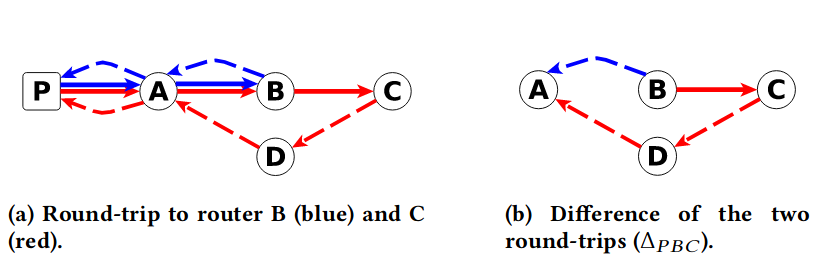
\includegraphics[width=0.7\linewidth]{illustrations/rtt-differ}
	\caption{}
	\label{fig:rtt-differ}
\end{figure}

\subsection{Le principe de la détection des changements des délais}

Le suivi du délai d'un lien est déduit du suivi de l'évolution de son RTT différentiel. Reprenons la formule du RTT différentiel du lien BC :  $\delta_{BC}$ + $\varepsilon_{PBC}$. Supposons qu'on dispose d'un nombre $n$ de sondes Atlas P$_i$, $i$ $\in$ [$1$, $n$], telles que toutes les sondes ont un chemin de retour différent depuis B et depuis C.  En effet, les RTTs différentiel pour chacune des sondes Atlas $\Delta_{P{_i}BC}$ partagent la même composante $\delta_{BC}$, toutefois, ces RTTs ont des valeurs des  $\varepsilon_{P_{i}BC}$ indépendantes. L'indépendance de ces valeurs implique que la distribution $\Delta_{P_{i}BC}$ est estimé d'être stable au cours du temps si $\delta_{BC}$ est constant. Cependant, un changement significatif de la valeur du $\delta_{BC}$ influence les valeurs des RTTs différentiel, dans ce cas, la distribution des RTTs différentiel changes si $\delta_{BC}$ change. Enfin, les changements des délais sont déduits des changements des RTTs différentiel qu'on peut les quantifier.

La détection des anomalies en délais repose sur un théorème très important en statistiques, c'est le théorème  central limite (TCL). Ce théorème  annonce que si on a une suite de variables aléatoires indépendantes ayant la même espérance et la même variance, la moyenne de ces variables aléatoires est une variable aléatoire qui suit une loi normale. De manière générale, le théorème central limite explique la distribution des moyennes des échantillons. Ce théorème peut être appliquer aux différents lois. Par exemple la loi normale \footnote{Un exemple illustratif dans \ref{appendix:clt-exemple}.}, binomiale, etc. 





\subsection{Les résultats de l'analyse des délais des liens}

Nous distinguons deux sortes de résultat à l'issu de l'analyse des changements des délais. Premièrement, ce sont les changements identifiés tout au long de la durée de l'analyse, chaque changement est caractérisé par un ensemble de détails. Pour le deuxième  résultat, ce sont des graphiques reprenant les changements ainsi que les changements jugés anormaux, ce qu'on va appeler par la suite par \textit{anomalies}, précisément ces graphiques présentent l'évolution du RTT différentiel d'un lien au cours du temps.

\subsection{Présentation de l'algorithme de la détection des changements anormaux : Résultat I}

\paragraph{Description de l'algorithme de détection} ~

Les étapes principales de la détection des changements des délais sont résumées dans l'algorithme \ref{algo:steps}. Nous allons détailler chaque étape : ses objectifs, ses entrées et ses sorties. En ce qui concerne l'entrée du programme principal, ce sont les paramètres présentés dans la section  \ref{par:parametre-de-lanalyse}.


\begin{algorithm}[H]

 	\begin{algorithmic}[1]
 		\Procedure{detectRttChangesMongo}{$expId$}
 		\ForAll {$currDate \in dates$}
 		\State computeRtt()
 		\State mergeRttResults()
 		\State outlierDetection()
 		\EndFor
 		\EndProcedure
 	\end{algorithmic}
 	\caption{Les étapes de la procédure detectRttChangesMongo()}
 	\label{algo:steps}
\end{algorithm}

\paragraph{Description des paramètres de l'analyse des délais} \label{par:parametre-de-lanalyse}~

La détection des changements des délais nécessite l'ajustement d'un nombre de paramètres. La valeur de chaque paramètre est relative au  fondement utilisé théorique ou bien empirique, qui a été  justifié par les auteurs du travail de référence.   Ci-dessous les paramètres à ajuster avant de lancer une analyse.  Chaque paramètre sera défini dans son contexte.

\subparagraph{start} : c'est la date de début de l'analyse. Ce sont les traceroutes capturés par les sondes Atlas à partir de cette date qui seront analysés.

\subparagraph{end} : c'est la date marquant la fin de l'analyse. Comme le paramètre \textit{start}, c'est la date des derniers traceroutes capturés par les sondes Atlas à considérer dans la présente analyse.

\subparagraph{timeWindow} :  ce paramètre est exprimé en seconde. La durée de l'analyse, qui est le temps écoulé entre \textit{start} et \textit{end}, est divisée sur des périodes de même taille : \textit{timeWindow}. Pour chacune de ces périodes, on caractérise les liens identifiés sur les traceroutes capturés en cette période. La figure \ref{fig:timewindow} reprend le contexte des trois paramètres \textit{start}, \textit{end} et \textit{timeWindow} avec les étapes principales.

\begin{figure}[h]
	
	\centering
	\resizebox{\textwidth}{!}{
		% Graphic for TeX using PGF
% Title: /home/bellafkih/Documents/2018-2019/memoire/rapport_memoire/dia/timewindow.dia
% Creator: Dia v0.97.3
% CreationDate: Sun Oct  7 15:34:20 2018
% For: bellafkih
% \usepackage{tikz}
% The following commands are not supported in PSTricks at present
% We define them conditionally, so when they are implemented,
% this pgf file will use them.
\ifx\du\undefined
  \newlength{\du}
\fi
\setlength{\du}{15\unitlength}
\begin{tikzpicture}
\pgftransformxscale{1.000000}
\pgftransformyscale{-1.000000}
\definecolor{dialinecolor}{rgb}{0.000000, 0.000000, 0.000000}
\pgfsetstrokecolor{dialinecolor}
\definecolor{dialinecolor}{rgb}{1.000000, 1.000000, 1.000000}
\pgfsetfillcolor{dialinecolor}
\pgfsetlinewidth{0.200000\du}
\pgfsetdash{}{0pt}
\pgfsetdash{}{0pt}
\pgfsetbuttcap
{
\definecolor{dialinecolor}{rgb}{0.000000, 0.000000, 0.000000}
\pgfsetfillcolor{dialinecolor}
% was here!!!
\pgfsetarrowsend{to}
\definecolor{dialinecolor}{rgb}{0.000000, 0.000000, 0.000000}
\pgfsetstrokecolor{dialinecolor}
\draw (10.000000\du,2.000000\du)--(10.000000\du,26.650000\du);
}
% setfont left to latex
\definecolor{dialinecolor}{rgb}{0.000000, 0.000000, 0.000000}
\pgfsetstrokecolor{dialinecolor}
\node[anchor=west] at (7.650000\du,2.050000\du){start};
% setfont left to latex
\definecolor{dialinecolor}{rgb}{0.000000, 0.000000, 0.000000}
\pgfsetstrokecolor{dialinecolor}
\node[anchor=west] at (7.850000\du,22.100000\du){end};
\pgfsetlinewidth{0.000000\du}
\pgfsetdash{}{0pt}
\pgfsetdash{}{0pt}
\pgfsetbuttcap
{
\definecolor{dialinecolor}{rgb}{0.000000, 0.000000, 0.000000}
\pgfsetfillcolor{dialinecolor}
% was here!!!
\definecolor{dialinecolor}{rgb}{0.000000, 0.000000, 0.000000}
\pgfsetstrokecolor{dialinecolor}
\draw (10.600000\du,2.000000\du)--(9.450000\du,2.000000\du);
}
\pgfsetlinewidth{0.000000\du}
\pgfsetdash{}{0pt}
\pgfsetdash{}{0pt}
\pgfsetbuttcap
{
\definecolor{dialinecolor}{rgb}{0.000000, 0.000000, 0.000000}
\pgfsetfillcolor{dialinecolor}
% was here!!!
\definecolor{dialinecolor}{rgb}{0.000000, 0.000000, 0.000000}
\pgfsetstrokecolor{dialinecolor}
\draw (10.585000\du,5.960000\du)--(9.435000\du,5.960000\du);
}
\pgfsetlinewidth{0.000000\du}
\pgfsetdash{}{0pt}
\pgfsetdash{}{0pt}
\pgfsetbuttcap
{
\definecolor{dialinecolor}{rgb}{0.000000, 0.000000, 0.000000}
\pgfsetfillcolor{dialinecolor}
% was here!!!
\definecolor{dialinecolor}{rgb}{0.000000, 0.000000, 0.000000}
\pgfsetstrokecolor{dialinecolor}
\draw (10.570000\du,10.020000\du)--(9.420000\du,10.020000\du);
}
\pgfsetlinewidth{0.000000\du}
\pgfsetdash{}{0pt}
\pgfsetdash{}{0pt}
\pgfsetbuttcap
{
\definecolor{dialinecolor}{rgb}{0.000000, 0.000000, 0.000000}
\pgfsetfillcolor{dialinecolor}
% was here!!!
\definecolor{dialinecolor}{rgb}{0.000000, 0.000000, 0.000000}
\pgfsetstrokecolor{dialinecolor}
\draw (10.505000\du,13.930000\du)--(9.355000\du,13.930000\du);
}
\pgfsetlinewidth{0.000000\du}
\pgfsetdash{}{0pt}
\pgfsetdash{}{0pt}
\pgfsetbuttcap
{
\definecolor{dialinecolor}{rgb}{0.000000, 0.000000, 0.000000}
\pgfsetfillcolor{dialinecolor}
% was here!!!
\definecolor{dialinecolor}{rgb}{0.000000, 0.000000, 0.000000}
\pgfsetstrokecolor{dialinecolor}
\draw (10.540000\du,17.940000\du)--(9.390000\du,17.940000\du);
}
\pgfsetlinewidth{0.000000\du}
\pgfsetdash{}{0pt}
\pgfsetdash{}{0pt}
\pgfsetbuttcap
{
\definecolor{dialinecolor}{rgb}{0.000000, 0.000000, 0.000000}
\pgfsetfillcolor{dialinecolor}
% was here!!!
\definecolor{dialinecolor}{rgb}{0.000000, 0.000000, 0.000000}
\pgfsetstrokecolor{dialinecolor}
\draw (10.575000\du,22.050000\du)--(9.425000\du,22.050000\du);
}
\pgfsetlinewidth{0.000000\du}
\pgfsetdash{}{0pt}
\pgfsetdash{}{0pt}
\pgfsetbuttcap
{
\definecolor{dialinecolor}{rgb}{0.000000, 0.000000, 0.000000}
\pgfsetfillcolor{dialinecolor}
% was here!!!
\pgfsetarrowsstart{to}
\pgfsetarrowsend{to}
\definecolor{dialinecolor}{rgb}{0.000000, 0.000000, 0.000000}
\pgfsetstrokecolor{dialinecolor}
\pgfpathmoveto{\pgfpoint{6.950071\du}{2.049940\du}}
\pgfpatharc{231}{129}{2.448949\du and 2.448949\du}
\pgfusepath{stroke}
}
% setfont left to latex
\definecolor{dialinecolor}{rgb}{0.000000, 0.000000, 0.000000}
\pgfsetstrokecolor{dialinecolor}
\node[anchor=west] at (2.150000\du,26.900000\du){Temps en secondes (s)};
\pgfsetlinewidth{0.000000\du}
\pgfsetdash{}{0pt}
\pgfsetdash{}{0pt}
\pgfsetbuttcap
{
\definecolor{dialinecolor}{rgb}{0.000000, 0.000000, 0.000000}
\pgfsetfillcolor{dialinecolor}
% was here!!!
\pgfsetarrowsstart{to}
\pgfsetarrowsend{to}
\definecolor{dialinecolor}{rgb}{0.000000, 0.000000, 0.000000}
\pgfsetstrokecolor{dialinecolor}
\pgfpathmoveto{\pgfpoint{7.049251\du}{6.119940\du}}
\pgfpatharc{231}{129}{2.448949\du and 2.448949\du}
\pgfusepath{stroke}
}
\pgfsetlinewidth{0.000000\du}
\pgfsetdash{}{0pt}
\pgfsetdash{}{0pt}
\pgfsetbuttcap
{
\definecolor{dialinecolor}{rgb}{0.000000, 0.000000, 0.000000}
\pgfsetfillcolor{dialinecolor}
% was here!!!
\pgfsetarrowsstart{to}
\pgfsetarrowsend{to}
\definecolor{dialinecolor}{rgb}{0.000000, 0.000000, 0.000000}
\pgfsetstrokecolor{dialinecolor}
\pgfpathmoveto{\pgfpoint{6.984251\du}{10.079940\du}}
\pgfpatharc{231}{129}{2.448949\du and 2.448949\du}
\pgfusepath{stroke}
}
\pgfsetlinewidth{0.000000\du}
\pgfsetdash{}{0pt}
\pgfsetdash{}{0pt}
\pgfsetbuttcap
{
\definecolor{dialinecolor}{rgb}{0.000000, 0.000000, 0.000000}
\pgfsetfillcolor{dialinecolor}
% was here!!!
\pgfsetarrowsstart{to}
\pgfsetarrowsend{to}
\definecolor{dialinecolor}{rgb}{0.000000, 0.000000, 0.000000}
\pgfsetstrokecolor{dialinecolor}
\pgfpathmoveto{\pgfpoint{6.869251\du}{14.089940\du}}
\pgfpatharc{231}{129}{2.448949\du and 2.448949\du}
\pgfusepath{stroke}
}
\pgfsetlinewidth{0.000000\du}
\pgfsetdash{}{0pt}
\pgfsetdash{}{0pt}
\pgfsetbuttcap
{
\definecolor{dialinecolor}{rgb}{0.000000, 0.000000, 0.000000}
\pgfsetfillcolor{dialinecolor}
% was here!!!
\pgfsetarrowsstart{to}
\pgfsetarrowsend{to}
\definecolor{dialinecolor}{rgb}{0.000000, 0.000000, 0.000000}
\pgfsetstrokecolor{dialinecolor}
\pgfpathmoveto{\pgfpoint{6.954251\du}{18.099940\du}}
\pgfpatharc{231}{129}{2.448949\du and 2.448949\du}
\pgfusepath{stroke}
}
% setfont left to latex
\definecolor{dialinecolor}{rgb}{0.000000, 0.000000, 0.000000}
\pgfsetstrokecolor{dialinecolor}
\node[anchor=west] at (0.650000\du,4.050000\du){timeWindow s};
% setfont left to latex
\definecolor{dialinecolor}{rgb}{0.000000, 0.000000, 0.000000}
\pgfsetstrokecolor{dialinecolor}
\node[anchor=west] at (0.685100\du,8.005000\du){timeWindow s};
% setfont left to latex
\definecolor{dialinecolor}{rgb}{0.000000, 0.000000, 0.000000}
\pgfsetstrokecolor{dialinecolor}
\node[anchor=west] at (0.870100\du,12.015000\du){timeWindow s};
% setfont left to latex
\definecolor{dialinecolor}{rgb}{0.000000, 0.000000, 0.000000}
\pgfsetstrokecolor{dialinecolor}
\node[anchor=west] at (0.905100\du,16.025000\du){timeWindow s};
% setfont left to latex
\definecolor{dialinecolor}{rgb}{0.000000, 0.000000, 0.000000}
\pgfsetstrokecolor{dialinecolor}
\node[anchor=west] at (1.040100\du,19.935000\du){timeWindow s};
% setfont left to latex
\definecolor{dialinecolor}{rgb}{0.000000, 0.000000, 0.000000}
\pgfsetstrokecolor{dialinecolor}
\node[anchor=west] at (11.200100\du,3.850000\du){appliquer : computeRtt(), mergeRttResults(), outlierDetection()};
% setfont left to latex
\definecolor{dialinecolor}{rgb}{0.000000, 0.000000, 0.000000}
\pgfsetstrokecolor{dialinecolor}
\node[anchor=west] at (11.035100\du,7.905000\du){appliquer : computeRtt(), mergeRttResults(), outlierDetection()};
% setfont left to latex
\definecolor{dialinecolor}{rgb}{0.000000, 0.000000, 0.000000}
\pgfsetstrokecolor{dialinecolor}
\node[anchor=west] at (11.120100\du,12.015000\du){appliquer : computeRtt(), mergeRttResults(), outlierDetection()};
% setfont left to latex
\definecolor{dialinecolor}{rgb}{0.000000, 0.000000, 0.000000}
\pgfsetstrokecolor{dialinecolor}
\node[anchor=west] at (11.105100\du,15.875000\du){appliquer : computeRtt(), mergeRttResults(), outlierDetection()};
% setfont left to latex
\definecolor{dialinecolor}{rgb}{0.000000, 0.000000, 0.000000}
\pgfsetstrokecolor{dialinecolor}
\node[anchor=west] at (11.040100\du,19.885000\du){appliquer : computeRtt(), mergeRttResults(), outlierDetection()};
% setfont left to latex
\definecolor{dialinecolor}{rgb}{0.000000, 0.000000, 0.000000}
\pgfsetstrokecolor{dialinecolor}
\node[anchor=west] at (11.950100\du,2.000000\du){inputs : paramère de l'expérience};
% setfont left to latex
\definecolor{dialinecolor}{rgb}{0.000000, 0.000000, 0.000000}
\pgfsetstrokecolor{dialinecolor}
\node[anchor=west] at (12.050100\du,22.000000\du){output : les changements détéctés et ses caractériqtiques};
\end{tikzpicture}
 
	}
	\caption{Illustration du paramètre timeWindow}
	\label{fig:timewindow}
\end{figure}


\subparagraph{alpha}: c'est le paramètre du lissage exponentiel.

\guillemotleft \textit{ Les méthodes de lissage exponentiel  sont un ensemble de techniques empiriques de prévision qui accordent plus ou moins d'importance aux valeurs du passé d'une série temporelle.\footnote{Source : \url{https://perso.math.univ-toulouse.fr/lagnoux/files/2013/12/Chap6.pdf}, consultée le $30/09/2018.$}} \guillemotright

Pour calculer la prochaine  valeur de la médiane des RTTs différentiel de référence $ \overline{m}_{t}$ du timeWindow  courant $ t $ , soit: 

 $m_t$ = $\Delta^{(m)}$ la médiane des RTTs différentiel observée pour un lien durant le timeWindow $t$. 
 
 $ \overline{m}_{t-1}$ = $ \overline{\Delta}^{(m)}$ est la médiane des  RTTs différentiel  de référence durant le timeWindow $ t-1 $,  la prochaine  valeur de la médiane de référence $ \overline{m}_{t}$ est obtenue par : 

\begin{center}
	$ \overline{m}_{t}$ =  $\alpha$ ${m}_{t}$ + (1-  $\alpha$) $ \overline{m}_{t-1}$
\end{center}

Le paramètre alpha $\alpha$, tel que  $\alpha \in (0, 1)$, est le seul paramètre à définir dans le calcul de $ \overline{m}_{t}$.  Ce paramètre contrôle l'importance  des mesures précédentes par rapport aux mesures récentes.

\guillemotleft \textit{Plus $\alpha$ est proche de $ 1 $ plus les observations récentes influent sur la prévision, à l'inverse un $\alpha$ proche de $0$ conduit à une prévision très stable prenant en compte un passé lointain. \footnote{Source : \url{https://www.math.u-psud.fr/~goude/Materials/time_series/cours3_lissage_expo.pdf}, consultée le $30/09/2018$.}}\guillemotright.  Dans la présente étude, le paramètre $\alpha$ est préféré d'être petit.





\subparagraph{minASN} : les paramètres \textit{minASN}, \textit{minASNEntropy} ainsi que  \textit{minSeen} dont les deux derniers seront détaillés dans la suite sont associés à l'aspect diversité des sondes Atlas pour assurer une exactitude des résultats obtenus.


L'analyse des RTTs différentiel est appliquée seulement sous certaines conditions. Ainsi, la détection des anomalies dans les délais d'un lien est valide si les éléments suivants sont vrais. (1) Le lien est surveillé par plusieurs sondes et que le chemin de retours vers ces sondes soit différent à chaque fois. (2) Les paquets ayant passés par le lien XY, doivent aussi passer par le lien XY en leur retour, mais dans le sens opposé. 

Les valeurs des RTTs ambiguës sont filtrées en éliminant les liens surveillés seulement par les sondes appartenant au même Système Autonome, car généralement le chemin de retour est similaire pour ces sondes suite à leur présence au sein du même Système Autonome (généralement même politique de routage). Seuls les liens surveillés par au moins $3$ Systèmes Autonomes qui sont conservés, la valeur de $3$ pour le paramètre \textit{minASN} est choisie de manière empirique. Sachant qu'une valeur plus petite que $3$ peut affecter l'exactitude des résultats. 





\subparagraph{minASNEntropy} : Il important qu'un lien soit identifié par au moins \textit{minASN} Systèmes Autonomes, toutefois, le nombre de sondes Atlas ayant identifié ce lien doit être équilibré entre ces Systèmes Autonomes.  En ce qui concerne l'équilibre du nombre de sondes ayant surveillé un lien par AS, il est mesuré par une entropie normalisée. Soit $A = \{ a_i \mid i \in [1, n] \}$, $ a_i $ est le nombre de sondes pour chaque AS parmi les n ASs surveillant un lien donné. L'entropie $H(A)$ est défini avec :

\begin{center}
	$H(A) =  - \frac{1}{\ln} \sum_{i=1}^{n} P(a_i) \ln P(a_i) $
\end{center}

Le nombre de sondes par Système Autonome sera équilibré jusqu'à l'atteinte de l'entropie minimale donnée par \textit{minASNEntropy}. L'idée est d'éliminer des sondes Atlas, de manière aléatoire, de l'AS qui a un grand nombre de sondes Atlas jusqu'à avoir l'équilibre mesuré par l'entropie.     Dans la présente analyse, les liens ayant une entropie $> 0.5$ sont conservés, cependant, si  l'entropie d'un lien est $< 0.5$,  chercher une sonde, de manière aléatoire, qui se trouve dans l'AS $i$ tel que $a_i = max (A)$, ensuite recalculer l'entropie avec la sonde. L'opération de l'élimination est répétée jusqu'à avoir une entropie $ > 0.5 $.

   \paragraph{L'entropie } \label{par:entrepie-sondes-par-as}~
   
\begin{tcolorbox}
\textit{\textbf{L'entropie} est une grandeur d'état extensive  qui caractérise l'état de désordre du système.} \footnote{Source : \url{ http://ressources.univ-lemans.fr/AccesLibre/UM/Pedago/chimie/01/03-Reaction_chimique/co/module_03-Reaction_chimique_26.html
   	}, consultée le $30/09/2018$.}
De faible valeurs d'entropie,$H(A) \backsimeq 0$ , indiquent que la majorité des sondes sont concentrées dans un seul AS, et les grandes valeurs d'entropie, $H(A) \backsimeq 1$, indiquent que les sondes sont réparties équitablement sur les ASs. 
\end{tcolorbox}
   


\subparagraph{minSeen} : comme l'analyse est faite sur plusieurs périodes : timeWindow, le paramètre \textit{minSeen} indique le nombre de fois où un lien a été identifié. Par exemple, un lien peut être identifié dans $3$ timeWindow, ou bien être identifié en une seule fois durant toute la période de l'analyse.

\subparagraph{af} : ce paramètre indique l'étendue de l'analyse des délais en matière de type d'adressage. Telle qu'une analyse peut concentrer sur les liens en IPv4 ou bien en IPv6. Pour précision, il est pris en compte  le type d'adressage IP lors du stockage des traceroutes dans MongoDB\footnote{C'est une base de données NoSQL utilisée dans le stockage des données dans le travail de référence.}. Ce que permet de choisir les traceroutes suivant ce paramètre\footnote{Dans MongoDB, la collection traceroute\_2017\_05\_15 reprend les traceroutes de la date 15/05/2017 en IPv4, et la collection traceroute6\_2017\_05\_15 pour la même date mais en IPv6.}. 

\subparagraph{comment} : un commentaire est utile pour donner plus d'informations sur une analyse en particulier. Les commentaires sont à titre informatifs et n'affectent pas l'analyse.

\subparagraph{prefixes} : les liens analysés sont finalement les liens entre deux routeurs adjacents dans la topologie. Avec l'expression régulière fournie à travers le paramètre \textit{prefixes}, il est possible de limiter l'analyse sur les liens où les routeurs appartiennent aux blocs d'adresses définis par \textit{prefixes}.  


\subparagraph{experimentDate} : le paramètre \textit{experimentDate} indique la date de lancement de l'expérience. Les auteurs enregistrent les expériences dans une collection dans la base de données MongoDB. Ce que permet de faciliter la comparaison entre les différentes expériences.

\subparagraph{confInterval} : 

\begin{tcolorbox}
	Afin de calculer l'incertitude associée à un ensemble de résultats, il faut répéter les mesures. Chaque mesure sur un échantillon peut donner des résultats différents. Ainsi, en se basant sur la déviation sur les résultats, il est possible de calculer l'incertitude de la "moyenne" calculée de ces résultats. Cette incertitude permet de donner une indication sur les données. Par exemple, est-ce que la moyenne calculée $N$ représente la valeur réelle avec une incertitude de plus ou moins  $m$?
\end{tcolorbox}
\begin{tcolorbox}
	   En statistiques, le \textit{binomial proportion confidence interval} est l'intervalle de confiance pour la probabilité de succès calculée à partir des séries d'expériences de succès-échec. C'est un intervalle qui estime la probabilité de succès $p$ si seulement le nombre d'expériences $n$ et celles réussites $n_s$ sont connus.
	   
	   Il existe plusieurs formules pour calculer l'intervalle de confiance binomial. Toutefois, elles se basent toutes sur une distribution binomiale.  Une distribution binomial s'applique si une expérience est répétée un nombre fixe de fois, chaque tentative a deux possibilités : succès ou échec. La probabilité est la même à chaque tentative et les tentatives sont statistiquement indépendantes. La distribution binomiale est une distribution de probabilité discrète, il est difficile de calculer pour un grand nombre de tentatives, il existe une variété d'approximations pour le calcul de l'intervalle de confiance.
	   
\end{tcolorbox}

les intervalles de confiance sont formulés par un calcul binomial avec distribution - free . Ce calcul  est approché par le score de Wilson. C'est une méthode pour calculer l'intervalle de confiance. Le score de Wilson fournit deux valeurs dans l'intervalle $ [0, 1]$. 


\paragraph{Intervalle de confiance d'une moyenne}~

L'intervalle de confiance (IC) est défini comme représentant les valeurs probables que peut prendre une moyenne, si l'on accepte une marge d'erreur définie à l'avance (e.g 5\%). Il existe plusieurs méthodes pour calculer l'intervalle de confiance d'une proportion. Parmi les critères impliqués sur le choix de la méthode de calcul, il y a N, le nombre total d'essais (nombre des expériences).

Dans le travail de référence, les auteurs ont utilisé la méthode du score de wilson pour calculer l'intervalle de confiance de la médiane\footnote{Le choix d'utilisation de la médiane à la place de la moyenne a été justifié dans le travail de référence.}.  Le score de wilson a montré ses performances même dans le cas où le nombre total d'essais est petit. Par exemple, il se peut qu'un lien soit caractérisé par seulement $ 3 $ RTTs différentiel durant un timeWindow. \footnote{Source : \url{http://npsycog.over-blog.com/article-3274585.html}, consultée le $ 12/10/2018 $.}

	 Chaque valeur de médiane a son intervalle de confiance. On compare le chevauchement entre l'intervalle de confiance de la médiane de référence avec l'intervalle de confiance de la valeur de médiane calculée en cours, d'un lien donné. Afin d'évaluer si la différence entre ces deux intervalles est significative statistiquement. En particulier une différence de $1$ $ms$ est non significative. On distingue trois cas comme illustré par la figure \ref{fig:illustration-cas-intervalles-deconfiance} et la formule \ref{equ:confidenceIntervalle}. 


\begin{figure}[H]
	\centering
	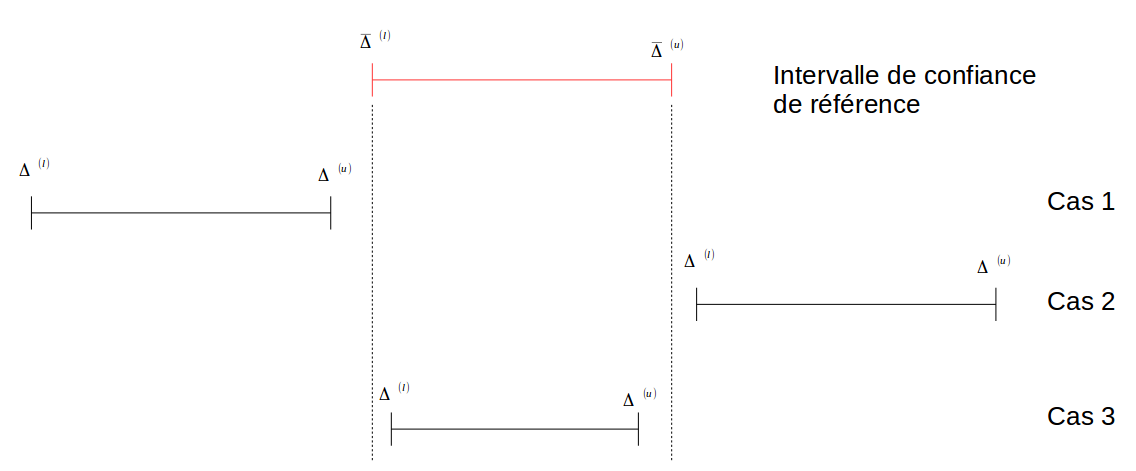
\includegraphics[width=1\linewidth]{illustrations/illustration-cas-intervalles-deconfiance}
	\caption{La comparaison entre les intervalles de confiance de la médiane de référence et de la médiane calculée.}
	\label{fig:illustration-cas-intervalles-deconfiance}
\end{figure}

Le cas $ 1 $ et $ 2 $ dans la figure 	\ref{fig:illustration-cas-intervalles-deconfiance} illustrent un changement anormal dans le délai du lien en question. Toutefois, le cas $ 3 $ où l'intervalle de confiance courant est inclus dans l'intervalle de référence, est le cas normal, autrement dit,  le délai de ce lien est normal. La différence entre les deux intervalles intervalles de confiance est quantifiée par la déviation $d$ définie par la formule \ref{equ:confidenceIntervalle}.

\begin{equation} \label{equ:confidenceIntervalle}
d=\begin{cases}
\frac{\Delta^{(l)} - \overline{\Delta}^{(u)}}{\overline{\Delta}^{(u)} - \overline{\Delta}^{(m)}}    , & \text{if $\overline{\Delta}^{(u)}<\Delta^{(l)}$}.\\

\frac{\overline{\Delta}^{(l)} - \Delta^{(u)}}{\overline{\Delta}^{(u)} - \overline{\Delta}^{(m)}}, & \text{if $\overline{\Delta}^{(m)}<\Delta^{(l)}$}.\\
0, & \text{otherwise}.
\end{cases}
\end{equation}

L'intervalle de confiance est calculé, dans la présente implémentation, avec la fonction  \textit{sm.stats.proportion\_confint}\footnote{Source : \url{https://www.statsmodels.org/dev/generated/statsmodels.stats.proportion.proportion_confint.html}, consultée le $ 07/10/2018 $.}.

\begin{lstlisting}[basicstyle=\tiny]
statsmodels.stats.proportion.proportion_confint(count, nobs, alpha=0.05, method='normal')
\end{lstlisting} 

\textit{proportion\_confint} est une implémentation, en python, pour le calcul du score de Wilson. Elle prend les paramètres suivants : 
\begin{itemize}
	\item count  : c'est le nombre de fois où une expérience  réussit.
	\item nobs : c'est le nombre total d'expériences.
	\item alpha : c'est le paramètre de risque. Généralement il prend les valeurs suivantes $ 5\% $, $ 1\% $ ou $ 0,1\% $. C'est un des paramètres de l'expérience.
	\item method: on distingue plusieurs méthodes, celle utilisée est \textit{wilson}.
\end{itemize}


En retour, la fonction \textit{proportion\_confint}  fournie \textit{ci\_low} et \textit{ci\_upp}. Ces deux grandeurs sont utilisés pour construire l'intervalle de confiance.
%, respectivement, ce sont les deux bord de l'intervalle de confiance  avec une probabilité  approximativement de  1-alpha.

%Un lien topologique, noté par (IP1, IP2),  

\subparagraph{Exemple des  paramètres de l'analyse des délais}~

\begin{lstlisting}[language=json,firstnumber=1,basicstyle=\tiny]
expParam = {
    	"timeWindow": 60*60, # in seconds 
    	"start": datetime(2018, 1, 1, 0, 0, tzinfo=timezone("UTC")), 
    	"end":   datetime(2018, 1, 1, 23, 0, tzinfo=timezone("UTC")),
    	"alpha": 0.01, 
    	"confInterval": 0.05,
    	"minASN": 3,
    	"minASNEntropy": 0.5,
    	"minSeen": 3,
    	"experimentDate": datetime.now(),
    	"af": "",
    	"comment": "some comment",
    	"prefixes": None
}
  \end{lstlisting}
   %or \small or \footnotesize etc.
   
   
  \paragraph{Les étapes de l'analyse des délais}~
  
  Les sections suivantes présentent chaque étape brièvement des étapes présentées dans l'algorithme 	\ref{algo:steps}, c'est pour l'illustration, car des détails peuvent manquer comme les paramètres des fonctions.
  \subparagraph{computeRtt} :
  
    \underline{Objectif} : identification de tout  lien dans les traceroutes analysés.
    
    \underline{Entrées} : af, start, end,  prefixes.
    
    \underline{Sorties} : la caractérisation des liens en calculant leur RTT différentiel.  

    \underline{Pseudo-code} : 
    
      \begin{algorithm}
      	\caption{caractérisation des liens }
      	\begin{algorithmic}[1]
      		\Function{computeRtt}{af, start, end, prefixes}
      		
      		\State $ diffRtt  \leftarrow   \{\} $
      		
      		\State $nbRow \leftarrow 0 $
      		
	  		\State $ traceroutes  \leftarrow  findTraceroutes(af, start, end, prefixes) $
	  		\ForAll {$trace \in traceroutes$}
		  		\State readOneTraceroute( $trace$ )
	  		\EndFor
	  		
	        \Return $ diffRtt $, $ nbRow $
      		\EndFunction
      	\end{algorithmic}

      	\label{algo:step-computeRtt}
      \end{algorithm}
      
      \underline{Description : }
      \begin{enumerate}
      	\item Rechercher les traceroutes, dans la base de données, capturés entre la date \textit{start} et \textit{end}, parmi les traceroutes ayant \textit{af} comme adressage. Si \textit{prefixes} est fixé, seuls les traceroutes ayant  impliqué des routeurs appartenant au bloc d'adresses défini par \textit{prefixes} qui seront conservés.
      	
      	\item Analyser chaque traceroute, \textit{trace}, à travers les étapes suivantes: 
      	\begin{enumerate}
      		\item élimination du traceroute échoué en vérifiant la présence des attributs "error" ou "err" dans les résultats de ce traceroute;
      		
      		\item si le traceroute n'a pas été éliminé durant l'étape précédente, on passe à l'évaluation de chaque saut. Un saut est éliminé si l'adresse IP est absente pour ce saut, s'il s'agit d'une adresse privée, si l'information sur le RTT est absente et enfin si le RTT a une valeur négative;
      		
      		\item caractérisation des liens en notons pour chaque couple d'adresses IP la distribution des RTTs, les sondes  Atlas et les identifiants des mesures. 
      	\end{enumerate}
      \end{enumerate}
      
   Soit un exemple illustratif des opérations décrites ci-dessus, la figure   \ref{fig:computertt} reprend les détails. Tel que :
   
   \begin{itemize}
   	\item Lien : lien à suivre, défini par deux adresses IP.
   	\item RTT différentiel : le RTT différentiel calculé du lien en question.
   	\item Probe : l'ensemble de sondes ayant surveillé le lien.
   	\item msmId : l'ensemble de mesures ayant surveillé le lien. Comme un identifiant de mesure définit la requête à lancer par toutes les sondes Atlas, ainsi, un lien peut être surveillé dans le cadre d'une mesure et avec une ou plusieurs sondes Atlas.
   \end{itemize}
   
   Pour le lien $ ('160.242.100.88', '196.216.48.144') $,  le calcul du RTT différentiel est décrit ci-dessous : 
    	\begin{align*}
    	RTT(160.242.100.88) & = 4.263; 6.082; 11.834 \\ 
    	mediane (4.263; 6.082; 11.834)&=  6.082 \\
    	RTT(160.242.100.88) &= 3.678; 15.568; 3.655\\
    	mediane(3.678; 15.568; 3.655)&= 3.678 \\
    	RTT Diff ('160.242.100.88', '196.216.48.144') &=  6.082 - 3.678  = 2,404
    	\end{align*}


    \begin{landscape}
    	\begin{figure}[H]
    		\centering
    		\resizebox{20cm}{!}{
    			% Graphic for TeX using PGF
% Title: /home/bellafkih/Documents/2018-2019/memoire/rapport_memoire/dia/traceroute-exemple.dia
% Creator: Dia v0.97.3
% CreationDate: Fri Oct  5 16:42:09 2018
% For: bellafkih
% \usepackage{tikz}
% The following commands are not supported in PSTricks at present
% We define them conditionally, so when they are implemented,
% this pgf file will use them.
\ifx\du\undefined
  \newlength{\du}
\fi
\setlength{\du}{15\unitlength}
\begin{tikzpicture}
\pgftransformxscale{1.000000}
\pgftransformyscale{-1.000000}
\definecolor{dialinecolor}{rgb}{0.000000, 0.000000, 0.000000}
\pgfsetstrokecolor{dialinecolor}
\definecolor{dialinecolor}{rgb}{1.000000, 1.000000, 1.000000}
\pgfsetfillcolor{dialinecolor}
\pgfsetlinewidth{0.000000\du}
\pgfsetdash{}{0pt}
\pgfsetdash{}{0pt}
\pgfsetbuttcap
\pgfsetmiterjoin
\pgfsetlinewidth{0.000000\du}
\pgfsetbuttcap
\pgfsetmiterjoin
\pgfsetdash{}{0pt}
\definecolor{dialinecolor}{rgb}{0.027451, 0.486275, 0.682353}
\pgfsetfillcolor{dialinecolor}
\pgfpathmoveto{\pgfpoint{-6.844583\du}{14.308835\du}}
\pgfpathlineto{\pgfpoint{-6.846043\du}{14.338043\du}}
\pgfpathlineto{\pgfpoint{-6.853345\du}{14.367981\du}}
\pgfpathlineto{\pgfpoint{-6.863568\du}{14.396458\du}}
\pgfpathlineto{\pgfpoint{-6.878171\du}{14.424571\du}}
\pgfpathlineto{\pgfpoint{-6.897522\du}{14.452683\du}}
\pgfpathlineto{\pgfpoint{-6.919427\du}{14.480065\du}}
\pgfpathlineto{\pgfpoint{-6.946079\du}{14.507082\du}}
\pgfpathlineto{\pgfpoint{-6.976748\du}{14.533369\du}}
\pgfpathlineto{\pgfpoint{-7.009606\du}{14.558561\du}}
\pgfpathlineto{\pgfpoint{-7.046846\du}{14.583753\du}}
\pgfpathlineto{\pgfpoint{-7.087737\du}{14.607849\du}}
\pgfpathlineto{\pgfpoint{-7.131549\du}{14.631215\du}}
\pgfpathlineto{\pgfpoint{-7.177916\du}{14.653851\du}}
\pgfpathlineto{\pgfpoint{-7.228299\du}{14.675757\du}}
\pgfpathlineto{\pgfpoint{-7.281238\du}{14.696568\du}}
\pgfpathlineto{\pgfpoint{-7.336733\du}{14.716648\du}}
\pgfpathlineto{\pgfpoint{-7.394783\du}{14.735998\du}}
\pgfpathlineto{\pgfpoint{-7.455389\du}{14.753888\du}}
\pgfpathlineto{\pgfpoint{-7.519281\du}{14.771047\du}}
\pgfpathlineto{\pgfpoint{-7.584269\du}{14.787477\du}}
\pgfpathlineto{\pgfpoint{-7.652907\du}{14.802446\du}}
\pgfpathlineto{\pgfpoint{-7.723736\du}{14.815954\du}}
\pgfpathlineto{\pgfpoint{-7.795660\du}{14.828733\du}}
\pgfpathlineto{\pgfpoint{-7.870504\du}{14.840781\du}}
\pgfpathlineto{\pgfpoint{-7.946445\du}{14.850639\du}}
\pgfpathlineto{\pgfpoint{-8.024940\du}{14.859766\du}}
\pgfpathlineto{\pgfpoint{-8.104531\du}{14.867433\du}}
\pgfpathlineto{\pgfpoint{-8.185583\du}{14.874005\du}}
\pgfpathlineto{\pgfpoint{-8.268825\du}{14.879116\du}}
\pgfpathlineto{\pgfpoint{-8.352432\du}{14.882767\du}}
\pgfpathlineto{\pgfpoint{-8.437865\du}{14.884958\du}}
\pgfpathlineto{\pgfpoint{-8.524393\du}{14.885688\du}}
\pgfpathlineto{\pgfpoint{-8.610556\du}{14.884958\du}}
\pgfpathlineto{\pgfpoint{-8.696353\du}{14.882767\du}}
\pgfpathlineto{\pgfpoint{-8.779960\du}{14.879116\du}}
\pgfpathlineto{\pgfpoint{-8.862837\du}{14.874005\du}}
\pgfpathlineto{\pgfpoint{-8.944254\du}{14.867433\du}}
\pgfpathlineto{\pgfpoint{-9.023845\du}{14.859766\du}}
\pgfpathlineto{\pgfpoint{-9.101611\du}{14.850639\du}}
\pgfpathlineto{\pgfpoint{-9.178281\du}{14.840781\du}}
\pgfpathlineto{\pgfpoint{-9.252396\du}{14.828733\du}}
\pgfpathlineto{\pgfpoint{-9.325050\du}{14.815954\du}}
\pgfpathlineto{\pgfpoint{-9.395514\du}{14.802446\du}}
\pgfpathlineto{\pgfpoint{-9.464152\du}{14.787477\du}}
\pgfpathlineto{\pgfpoint{-9.529869\du}{14.771047\du}}
\pgfpathlineto{\pgfpoint{-9.593396\du}{14.753888\du}}
\pgfpathlineto{\pgfpoint{-9.654367\du}{14.735998\du}}
\pgfpathlineto{\pgfpoint{-9.712783\du}{14.716648\du}}
\pgfpathlineto{\pgfpoint{-9.767912\du}{14.696568\du}}
\pgfpathlineto{\pgfpoint{-9.820851\du}{14.675757\du}}
\pgfpathlineto{\pgfpoint{-9.870870\du}{14.653851\du}}
\pgfpathlineto{\pgfpoint{-9.917967\du}{14.631215\du}}
\pgfpathlineto{\pgfpoint{-9.961414\du}{14.607849\du}}
\pgfpathlineto{\pgfpoint{-10.002304\du}{14.583753\du}}
\pgfpathlineto{\pgfpoint{-10.039544\du}{14.558561\du}}
\pgfpathlineto{\pgfpoint{-10.072768\du}{14.533369\du}}
\pgfpathlineto{\pgfpoint{-10.103071\du}{14.507082\du}}
\pgfpathlineto{\pgfpoint{-10.129723\du}{14.480065\du}}
\pgfpathlineto{\pgfpoint{-10.151629\du}{14.452683\du}}
\pgfpathlineto{\pgfpoint{-10.170979\du}{14.424571\du}}
\pgfpathlineto{\pgfpoint{-10.185583\du}{14.396458\du}}
\pgfpathlineto{\pgfpoint{-10.196171\du}{14.367981\du}}
\pgfpathlineto{\pgfpoint{-10.203108\du}{14.338043\du}}
\pgfpathlineto{\pgfpoint{-10.204933\du}{14.308835\du}}
\pgfpathlineto{\pgfpoint{-10.203108\du}{14.278897\du}}
\pgfpathlineto{\pgfpoint{-10.196171\du}{14.249689\du}}
\pgfpathlineto{\pgfpoint{-10.185583\du}{14.220482\du}}
\pgfpathlineto{\pgfpoint{-10.170979\du}{14.192369\du}}
\pgfpathlineto{\pgfpoint{-10.151629\du}{14.164257\du}}
\pgfpathlineto{\pgfpoint{-10.129723\du}{14.136874\du}}
\pgfpathlineto{\pgfpoint{-10.103071\du}{14.110222\du}}
\pgfpathlineto{\pgfpoint{-10.072768\du}{14.083935\du}}
\pgfpathlineto{\pgfpoint{-10.039544\du}{14.058379\du}}
\pgfpathlineto{\pgfpoint{-10.002304\du}{14.033552\du}}
\pgfpathlineto{\pgfpoint{-9.961414\du}{14.009091\du}}
\pgfpathlineto{\pgfpoint{-9.917967\du}{13.985724\du}}
\pgfpathlineto{\pgfpoint{-9.870870\du}{13.963453\du}}
\pgfpathlineto{\pgfpoint{-9.820851\du}{13.941183\du}}
\pgfpathlineto{\pgfpoint{-9.767912\du}{13.920372\du}}
\pgfpathlineto{\pgfpoint{-9.712783\du}{13.900292\du}}
\pgfpathlineto{\pgfpoint{-9.654367\du}{13.881672\du}}
\pgfpathlineto{\pgfpoint{-9.593396\du}{13.862687\du}}
\pgfpathlineto{\pgfpoint{-9.529869\du}{13.845892\du}}
\pgfpathlineto{\pgfpoint{-9.464152\du}{13.830193\du}}
\pgfpathlineto{\pgfpoint{-9.395514\du}{13.814859\du}}
\pgfpathlineto{\pgfpoint{-9.325050\du}{13.800985\du}}
\pgfpathlineto{\pgfpoint{-9.252396\du}{13.787842\du}}
\pgfpathlineto{\pgfpoint{-9.178281\du}{13.776889\du}}
\pgfpathlineto{\pgfpoint{-9.101611\du}{13.766301\du}}
\pgfpathlineto{\pgfpoint{-9.023845\du}{13.756809\du}}
\pgfpathlineto{\pgfpoint{-8.944254\du}{13.749507\du}}
\pgfpathlineto{\pgfpoint{-8.862837\du}{13.742935\du}}
\pgfpathlineto{\pgfpoint{-8.779960\du}{13.737824\du}}
\pgfpathlineto{\pgfpoint{-8.696353\du}{13.734173\du}}
\pgfpathlineto{\pgfpoint{-8.610556\du}{13.732347\du}}
\pgfpathlineto{\pgfpoint{-8.524393\du}{13.731252\du}}
\pgfpathlineto{\pgfpoint{-8.437865\du}{13.732347\du}}
\pgfpathlineto{\pgfpoint{-8.352432\du}{13.734173\du}}
\pgfpathlineto{\pgfpoint{-8.268825\du}{13.737824\du}}
\pgfpathlineto{\pgfpoint{-8.185583\du}{13.742935\du}}
\pgfpathlineto{\pgfpoint{-8.104531\du}{13.749507\du}}
\pgfpathlineto{\pgfpoint{-8.024940\du}{13.756809\du}}
\pgfpathlineto{\pgfpoint{-7.946445\du}{13.766301\du}}
\pgfpathlineto{\pgfpoint{-7.870504\du}{13.776889\du}}
\pgfpathlineto{\pgfpoint{-7.795660\du}{13.787842\du}}
\pgfpathlineto{\pgfpoint{-7.723736\du}{13.800985\du}}
\pgfpathlineto{\pgfpoint{-7.652907\du}{13.814859\du}}
\pgfpathlineto{\pgfpoint{-7.584269\du}{13.830193\du}}
\pgfpathlineto{\pgfpoint{-7.519281\du}{13.845892\du}}
\pgfpathlineto{\pgfpoint{-7.455389\du}{13.862687\du}}
\pgfpathlineto{\pgfpoint{-7.394783\du}{13.881672\du}}
\pgfpathlineto{\pgfpoint{-7.336733\du}{13.900292\du}}
\pgfpathlineto{\pgfpoint{-7.281238\du}{13.920372\du}}
\pgfpathlineto{\pgfpoint{-7.228299\du}{13.941183\du}}
\pgfpathlineto{\pgfpoint{-7.177916\du}{13.963453\du}}
\pgfpathlineto{\pgfpoint{-7.131549\du}{13.985724\du}}
\pgfpathlineto{\pgfpoint{-7.087737\du}{14.009091\du}}
\pgfpathlineto{\pgfpoint{-7.046846\du}{14.033552\du}}
\pgfpathlineto{\pgfpoint{-7.009606\du}{14.058379\du}}
\pgfpathlineto{\pgfpoint{-6.976748\du}{14.083935\du}}
\pgfpathlineto{\pgfpoint{-6.946079\du}{14.110222\du}}
\pgfpathlineto{\pgfpoint{-6.919427\du}{14.136874\du}}
\pgfpathlineto{\pgfpoint{-6.897522\du}{14.164257\du}}
\pgfpathlineto{\pgfpoint{-6.878171\du}{14.192369\du}}
\pgfpathlineto{\pgfpoint{-6.863568\du}{14.220482\du}}
\pgfpathlineto{\pgfpoint{-6.853345\du}{14.249689\du}}
\pgfpathlineto{\pgfpoint{-6.846043\du}{14.278897\du}}
\pgfpathlineto{\pgfpoint{-6.844583\du}{14.308835\du}}
\pgfusepath{fill}
\pgfsetlinewidth{0.000000\du}
\pgfsetbuttcap
\pgfsetmiterjoin
\pgfsetdash{}{0pt}
\definecolor{dialinecolor}{rgb}{0.678431, 0.839216, 0.905882}
\pgfsetfillcolor{dialinecolor}
\pgfpathmoveto{\pgfpoint{-8.524393\du}{14.896276\du}}
\pgfpathlineto{\pgfpoint{-8.524393\du}{14.896276\du}}
\pgfpathlineto{\pgfpoint{-8.480946\du}{14.896276\du}}
\pgfpathlineto{\pgfpoint{-8.437500\du}{14.895545\du}}
\pgfpathlineto{\pgfpoint{-8.394418\du}{14.894450\du}}
\pgfpathlineto{\pgfpoint{-8.352432\du}{14.893355\du}}
\pgfpathlineto{\pgfpoint{-8.309716\du}{14.891529\du}}
\pgfpathlineto{\pgfpoint{-8.268095\du}{14.889339\du}}
\pgfpathlineto{\pgfpoint{-8.226474\du}{14.886783\du}}
\pgfpathlineto{\pgfpoint{-8.184853\du}{14.884593\du}}
\pgfpathlineto{\pgfpoint{-8.144327\du}{14.881672\du}}
\pgfpathlineto{\pgfpoint{-8.103436\du}{14.878021\du}}
\pgfpathlineto{\pgfpoint{-8.063641\du}{14.874005\du}}
\pgfpathlineto{\pgfpoint{-8.023480\du}{14.869989\du}}
\pgfpathlineto{\pgfpoint{-7.984780\du}{14.865607\du}}
\pgfpathlineto{\pgfpoint{-7.945349\du}{14.861226\du}}
\pgfpathlineto{\pgfpoint{-7.907379\du}{14.855750\du}}
\pgfpathlineto{\pgfpoint{-7.868314\du}{14.850639\du}}
\pgfpathlineto{\pgfpoint{-7.831074\du}{14.845162\du}}
\pgfpathlineto{\pgfpoint{-7.794199\du}{14.838955\du}}
\pgfpathlineto{\pgfpoint{-7.757690\du}{14.833114\du}}
\pgfpathlineto{\pgfpoint{-7.721180\du}{14.826542\du}}
\pgfpathlineto{\pgfpoint{-7.685765\du}{14.819605\du}}
\pgfpathlineto{\pgfpoint{-7.651081\du}{14.812668\du}}
\pgfpathlineto{\pgfpoint{-7.616397\du}{14.805001\du}}
\pgfpathlineto{\pgfpoint{-7.582443\du}{14.797334\du}}
\pgfpathlineto{\pgfpoint{-7.548854\du}{14.788937\du}}
\pgfpathlineto{\pgfpoint{-7.515995\du}{14.780905\du}}
\pgfpathlineto{\pgfpoint{-7.484232\du}{14.772873\du}}
\pgfpathlineto{\pgfpoint{-7.452834\du}{14.764111\du}}
\pgfpathlineto{\pgfpoint{-7.437500\du}{14.759364\du}}
\pgfpathlineto{\pgfpoint{-7.422166\du}{14.755348\du}}
\pgfpathlineto{\pgfpoint{-7.406101\du}{14.750602\du}}
\pgfpathlineto{\pgfpoint{-7.391497\du}{14.745856\du}}
\pgfpathlineto{\pgfpoint{-7.377259\du}{14.741110\du}}
\pgfpathlineto{\pgfpoint{-7.362290\du}{14.735998\du}}
\pgfpathlineto{\pgfpoint{-7.347321\du}{14.731252\du}}
\pgfpathlineto{\pgfpoint{-7.333447\du}{14.726506\du}}
\pgfpathlineto{\pgfpoint{-7.319208\du}{14.721394\du}}
\pgfpathlineto{\pgfpoint{-7.305335\du}{14.716648\du}}
\pgfpathlineto{\pgfpoint{-7.291096\du}{14.711172\du}}
\pgfpathlineto{\pgfpoint{-7.277952\du}{14.706790\du}}
\pgfpathlineto{\pgfpoint{-7.263714\du}{14.701314\du}}
\pgfpathlineto{\pgfpoint{-7.250570\du}{14.696203\du}}
\pgfpathlineto{\pgfpoint{-7.237427\du}{14.690726\du}}
\pgfpathlineto{\pgfpoint{-7.223918\du}{14.684885\du}}
\pgfpathlineto{\pgfpoint{-7.211140\du}{14.679773\du}}
\pgfpathlineto{\pgfpoint{-7.199092\du}{14.674297\du}}
\pgfpathlineto{\pgfpoint{-7.186313\du}{14.668455\du}}
\pgfpathlineto{\pgfpoint{-7.173900\du}{14.663344\du}}
\pgfpathlineto{\pgfpoint{-7.161487\du}{14.657502\du}}
\pgfpathlineto{\pgfpoint{-7.150169\du}{14.652026\du}}
\pgfpathlineto{\pgfpoint{-7.138120\du}{14.646184\du}}
\pgfpathlineto{\pgfpoint{-7.127167\du}{14.640343\du}}
\pgfpathlineto{\pgfpoint{-7.115484\du}{14.634501\du}}
\pgfpathlineto{\pgfpoint{-7.104166\du}{14.628660\du}}
\pgfpathlineto{\pgfpoint{-7.092848\du}{14.622818\du}}
\pgfpathlineto{\pgfpoint{-7.082261\du}{14.616612\du}}
\pgfpathlineto{\pgfpoint{-7.072403\du}{14.610770\du}}
\pgfpathlineto{\pgfpoint{-7.061815\du}{14.604928\du}}
\pgfpathlineto{\pgfpoint{-7.051592\du}{14.598357\du}}
\pgfpathlineto{\pgfpoint{-7.041735\du}{14.592515\du}}
\pgfpathlineto{\pgfpoint{-7.031877\du}{14.585943\du}}
\pgfpathlineto{\pgfpoint{-7.022750\du}{14.579737\du}}
\pgfpathlineto{\pgfpoint{-7.013622\du}{14.573165\du}}
\pgfpathlineto{\pgfpoint{-7.004130\du}{14.567323\du}}
\pgfpathlineto{\pgfpoint{-6.995368\du}{14.560752\du}}
\pgfpathlineto{\pgfpoint{-6.986240\du}{14.554545\du}}
\pgfpathlineto{\pgfpoint{-6.978208\du}{14.547973\du}}
\pgfpathlineto{\pgfpoint{-6.969446\du}{14.541036\du}}
\pgfpathlineto{\pgfpoint{-6.962144\du}{14.534465\du}}
\pgfpathlineto{\pgfpoint{-6.954112\du}{14.528258\du}}
\pgfpathlineto{\pgfpoint{-6.946079\du}{14.520956\du}}
\pgfpathlineto{\pgfpoint{-6.939508\du}{14.514750\du}}
\pgfpathlineto{\pgfpoint{-6.932206\du}{14.507813\du}}
\pgfpathlineto{\pgfpoint{-6.925634\du}{14.500511\du}}
\pgfpathlineto{\pgfpoint{-6.918697\du}{14.494304\du}}
\pgfpathlineto{\pgfpoint{-6.912125\du}{14.487367\du}}
\pgfpathlineto{\pgfpoint{-6.905919\du}{14.480065\du}}
\pgfpathlineto{\pgfpoint{-6.900077\du}{14.473128\du}}
\pgfpathlineto{\pgfpoint{-6.894601\du}{14.466192\du}}
\pgfpathlineto{\pgfpoint{-6.888759\du}{14.459255\du}}
\pgfpathlineto{\pgfpoint{-6.884013\du}{14.451953\du}}
\pgfpathlineto{\pgfpoint{-6.878537\du}{14.444651\du}}
\pgfpathlineto{\pgfpoint{-6.873790\du}{14.437349\du}}
\pgfpathlineto{\pgfpoint{-6.869409\du}{14.430412\du}}
\pgfpathlineto{\pgfpoint{-6.865393\du}{14.422745\du}}
\pgfpathlineto{\pgfpoint{-6.861377\du}{14.415808\du}}
\pgfpathlineto{\pgfpoint{-6.858091\du}{14.408141\du}}
\pgfpathlineto{\pgfpoint{-6.854075\du}{14.400474\du}}
\pgfpathlineto{\pgfpoint{-6.850789\du}{14.392807\du}}
\pgfpathlineto{\pgfpoint{-6.848234\du}{14.385505\du}}
\pgfpathlineto{\pgfpoint{-6.845313\du}{14.378203\du}}
\pgfpathlineto{\pgfpoint{-6.843487\du}{14.370901\du}}
\pgfpathlineto{\pgfpoint{-6.840566\du}{14.363234\du}}
\pgfpathlineto{\pgfpoint{-6.839471\du}{14.354837\du}}
\pgfpathlineto{\pgfpoint{-6.837281\du}{14.347170\du}}
\pgfpathlineto{\pgfpoint{-6.836185\du}{14.339868\du}}
\pgfpathlineto{\pgfpoint{-6.835455\du}{14.332201\du}}
\pgfpathlineto{\pgfpoint{-6.834725\du}{14.323804\du}}
\pgfpathlineto{\pgfpoint{-6.833995\du}{14.316502\du}}
\pgfpathlineto{\pgfpoint{-6.833995\du}{14.308835\du}}
\pgfpathlineto{\pgfpoint{-6.854075\du}{14.308835\du}}
\pgfpathlineto{\pgfpoint{-6.854805\du}{14.315772\du}}
\pgfpathlineto{\pgfpoint{-6.854805\du}{14.322709\du}}
\pgfpathlineto{\pgfpoint{-6.855170\du}{14.329645\du}}
\pgfpathlineto{\pgfpoint{-6.856996\du}{14.336947\du}}
\pgfpathlineto{\pgfpoint{-6.858091\du}{14.343884\du}}
\pgfpathlineto{\pgfpoint{-6.858821\du}{14.350821\du}}
\pgfpathlineto{\pgfpoint{-6.861012\du}{14.357758\du}}
\pgfpathlineto{\pgfpoint{-6.862472\du}{14.365060\du}}
\pgfpathlineto{\pgfpoint{-6.864663\du}{14.371266\du}}
\pgfpathlineto{\pgfpoint{-6.867219\du}{14.378203\du}}
\pgfpathlineto{\pgfpoint{-6.870139\du}{14.385505\du}}
\pgfpathlineto{\pgfpoint{-6.872695\du}{14.392442\du}}
\pgfpathlineto{\pgfpoint{-6.876711\du}{14.399379\du}}
\pgfpathlineto{\pgfpoint{-6.879632\du}{14.405951\du}}
\pgfpathlineto{\pgfpoint{-6.883648\du}{14.412888\du}}
\pgfpathlineto{\pgfpoint{-6.886569\du}{14.419459\du}}
\pgfpathlineto{\pgfpoint{-6.890950\du}{14.426396\du}}
\pgfpathlineto{\pgfpoint{-6.895331\du}{14.433333\du}}
\pgfpathlineto{\pgfpoint{-6.900077\du}{14.439905\du}}
\pgfpathlineto{\pgfpoint{-6.905189\du}{14.446111\du}}
\pgfpathlineto{\pgfpoint{-6.909935\du}{14.453413\du}}
\pgfpathlineto{\pgfpoint{-6.916142\du}{14.460350\du}}
\pgfpathlineto{\pgfpoint{-6.921618\du}{14.466557\du}}
\pgfpathlineto{\pgfpoint{-6.926729\du}{14.473128\du}}
\pgfpathlineto{\pgfpoint{-6.933301\du}{14.479700\du}}
\pgfpathlineto{\pgfpoint{-6.940238\du}{14.486637\du}}
\pgfpathlineto{\pgfpoint{-6.946079\du}{14.493209\du}}
\pgfpathlineto{\pgfpoint{-6.953381\du}{14.499415\du}}
\pgfpathlineto{\pgfpoint{-6.959953\du}{14.505987\du}}
\pgfpathlineto{\pgfpoint{-6.967620\du}{14.512194\du}}
\pgfpathlineto{\pgfpoint{-6.974922\du}{14.518766\du}}
\pgfpathlineto{\pgfpoint{-6.982954\du}{14.525337\du}}
\pgfpathlineto{\pgfpoint{-6.990621\du}{14.531544\du}}
\pgfpathlineto{\pgfpoint{-6.999384\du}{14.538116\du}}
\pgfpathlineto{\pgfpoint{-7.007781\du}{14.543957\du}}
\pgfpathlineto{\pgfpoint{-7.016543\du}{14.550529\du}}
\pgfpathlineto{\pgfpoint{-7.024575\du}{14.556736\du}}
\pgfpathlineto{\pgfpoint{-7.033338\du}{14.562577\du}}
\pgfpathlineto{\pgfpoint{-7.042830\du}{14.569149\du}}
\pgfpathlineto{\pgfpoint{-7.053053\du}{14.574990\du}}
\pgfpathlineto{\pgfpoint{-7.062180\du}{14.581562\du}}
\pgfpathlineto{\pgfpoint{-7.072403\du}{14.587404\du}}
\pgfpathlineto{\pgfpoint{-7.082261\du}{14.593245\du}}
\pgfpathlineto{\pgfpoint{-7.092118\du}{14.599087\du}}
\pgfpathlineto{\pgfpoint{-7.103071\du}{14.604928\du}}
\pgfpathlineto{\pgfpoint{-7.114024\du}{14.610770\du}}
\pgfpathlineto{\pgfpoint{-7.124247\du}{14.616612\du}}
\pgfpathlineto{\pgfpoint{-7.136295\du}{14.622453\du}}
\pgfpathlineto{\pgfpoint{-7.146883\du}{14.627564\du}}
\pgfpathlineto{\pgfpoint{-7.158931\du}{14.633406\du}}
\pgfpathlineto{\pgfpoint{-7.170249\du}{14.639248\du}}
\pgfpathlineto{\pgfpoint{-7.182662\du}{14.644724\du}}
\pgfpathlineto{\pgfpoint{-7.194710\du}{14.649835\du}}
\pgfpathlineto{\pgfpoint{-7.207124\du}{14.655677\du}}
\pgfpathlineto{\pgfpoint{-7.219172\du}{14.661153\du}}
\pgfpathlineto{\pgfpoint{-7.232315\du}{14.666265\du}}
\pgfpathlineto{\pgfpoint{-7.245094\du}{14.671376\du}}
\pgfpathlineto{\pgfpoint{-7.257872\du}{14.676852\du}}
\pgfpathlineto{\pgfpoint{-7.271016\du}{14.681964\du}}
\pgfpathlineto{\pgfpoint{-7.284524\du}{14.687440\du}}
\pgfpathlineto{\pgfpoint{-7.297668\du}{14.691821\du}}
\pgfpathlineto{\pgfpoint{-7.311906\du}{14.697298\du}}
\pgfpathlineto{\pgfpoint{-7.325780\du}{14.702044\du}}
\pgfpathlineto{\pgfpoint{-7.340019\du}{14.707156\du}}
\pgfpathlineto{\pgfpoint{-7.354623\du}{14.711902\du}}
\pgfpathlineto{\pgfpoint{-7.368496\du}{14.716648\du}}
\pgfpathlineto{\pgfpoint{-7.383100\du}{14.721394\du}}
\pgfpathlineto{\pgfpoint{-7.397339\du}{14.725775\du}}
\pgfpathlineto{\pgfpoint{-7.413038\du}{14.730522\du}}
\pgfpathlineto{\pgfpoint{-7.427277\du}{14.735268\du}}
\pgfpathlineto{\pgfpoint{-7.442976\du}{14.740014\du}}
\pgfpathlineto{\pgfpoint{-7.457945\du}{14.744030\du}}
\pgfpathlineto{\pgfpoint{-7.489343\du}{14.752793\du}}
\pgfpathlineto{\pgfpoint{-7.521472\du}{14.761190\du}}
\pgfpathlineto{\pgfpoint{-7.553600\du}{14.769222\du}}
\pgfpathlineto{\pgfpoint{-7.586824\du}{14.777254\du}}
\pgfpathlineto{\pgfpoint{-7.621143\du}{14.784921\du}}
\pgfpathlineto{\pgfpoint{-7.655097\du}{14.792223\du}}
\pgfpathlineto{\pgfpoint{-7.689782\du}{14.799160\du}}
\pgfpathlineto{\pgfpoint{-7.725561\du}{14.806097\du}}
\pgfpathlineto{\pgfpoint{-7.760975\du}{14.812668\du}}
\pgfpathlineto{\pgfpoint{-7.797850\du}{14.818875\du}}
\pgfpathlineto{\pgfpoint{-7.834360\du}{14.824717\du}}
\pgfpathlineto{\pgfpoint{-7.871600\du}{14.830558\du}}
\pgfpathlineto{\pgfpoint{-7.909205\du}{14.836035\du}}
\pgfpathlineto{\pgfpoint{-7.947905\du}{14.840781\du}}
\pgfpathlineto{\pgfpoint{-7.986605\du}{14.845162\du}}
\pgfpathlineto{\pgfpoint{-8.026036\du}{14.849908\du}}
\pgfpathlineto{\pgfpoint{-8.065101\du}{14.853559\du}}
\pgfpathlineto{\pgfpoint{-8.105262\du}{14.857575\du}}
\pgfpathlineto{\pgfpoint{-8.145422\du}{14.860496\du}}
\pgfpathlineto{\pgfpoint{-8.186678\du}{14.864147\du}}
\pgfpathlineto{\pgfpoint{-8.227569\du}{14.867068\du}}
\pgfpathlineto{\pgfpoint{-8.268825\du}{14.869258\du}}
\pgfpathlineto{\pgfpoint{-8.310446\du}{14.871084\du}}
\pgfpathlineto{\pgfpoint{-8.353162\du}{14.872909\du}}
\pgfpathlineto{\pgfpoint{-8.395879\du}{14.874005\du}}
\pgfpathlineto{\pgfpoint{-8.437865\du}{14.875100\du}}
\pgfpathlineto{\pgfpoint{-8.481311\du}{14.875100\du}}
\pgfpathlineto{\pgfpoint{-8.524393\du}{14.875830\du}}
\pgfpathlineto{\pgfpoint{-8.524393\du}{14.875830\du}}
\pgfpathlineto{\pgfpoint{-8.524393\du}{14.875830\du}}
\pgfpathlineto{\pgfpoint{-8.525123\du}{14.875830\du}}
\pgfpathlineto{\pgfpoint{-8.526948\du}{14.875830\du}}
\pgfpathlineto{\pgfpoint{-8.528044\du}{14.876195\du}}
\pgfpathlineto{\pgfpoint{-8.528774\du}{14.876195\du}}
\pgfpathlineto{\pgfpoint{-8.529139\du}{14.876925\du}}
\pgfpathlineto{\pgfpoint{-8.530599\du}{14.877291\du}}
\pgfpathlineto{\pgfpoint{-8.531330\du}{14.878021\du}}
\pgfpathlineto{\pgfpoint{-8.532060\du}{14.878751\du}}
\pgfpathlineto{\pgfpoint{-8.533155\du}{14.880576\du}}
\pgfpathlineto{\pgfpoint{-8.533885\du}{14.882037\du}}
\pgfpathlineto{\pgfpoint{-8.533885\du}{14.883862\du}}
\pgfpathlineto{\pgfpoint{-8.534615\du}{14.885688\du}}
\pgfpathlineto{\pgfpoint{-8.533885\du}{14.887878\du}}
\pgfpathlineto{\pgfpoint{-8.533885\du}{14.889704\du}}
\pgfpathlineto{\pgfpoint{-8.533155\du}{14.891529\du}}
\pgfpathlineto{\pgfpoint{-8.532060\du}{14.893355\du}}
\pgfpathlineto{\pgfpoint{-8.531330\du}{14.893720\du}}
\pgfpathlineto{\pgfpoint{-8.530599\du}{14.894450\du}}
\pgfpathlineto{\pgfpoint{-8.529139\du}{14.895180\du}}
\pgfpathlineto{\pgfpoint{-8.528774\du}{14.895545\du}}
\pgfpathlineto{\pgfpoint{-8.528044\du}{14.895545\du}}
\pgfpathlineto{\pgfpoint{-8.526948\du}{14.896276\du}}
\pgfpathlineto{\pgfpoint{-8.525123\du}{14.896276\du}}
\pgfpathlineto{\pgfpoint{-8.524393\du}{14.896276\du}}
\pgfusepath{fill}
\pgfsetbuttcap
\pgfsetmiterjoin
\pgfsetdash{}{0pt}
\definecolor{dialinecolor}{rgb}{0.678431, 0.839216, 0.905882}
\pgfsetfillcolor{dialinecolor}
\pgfpathmoveto{\pgfpoint{-10.215156\du}{14.308835\du}}
\pgfpathlineto{\pgfpoint{-10.215156\du}{14.308835\du}}
\pgfpathlineto{\pgfpoint{-10.215156\du}{14.316502\du}}
\pgfpathlineto{\pgfpoint{-10.214791\du}{14.323804\du}}
\pgfpathlineto{\pgfpoint{-10.214060\du}{14.332201\du}}
\pgfpathlineto{\pgfpoint{-10.212965\du}{14.339868\du}}
\pgfpathlineto{\pgfpoint{-10.211870\du}{14.347170\du}}
\pgfpathlineto{\pgfpoint{-10.210044\du}{14.354837\du}}
\pgfpathlineto{\pgfpoint{-10.208219\du}{14.363234\du}}
\pgfpathlineto{\pgfpoint{-10.206028\du}{14.370901\du}}
\pgfpathlineto{\pgfpoint{-10.203838\du}{14.378203\du}}
\pgfpathlineto{\pgfpoint{-10.201282\du}{14.385505\du}}
\pgfpathlineto{\pgfpoint{-10.198361\du}{14.392807\du}}
\pgfpathlineto{\pgfpoint{-10.194710\du}{14.400474\du}}
\pgfpathlineto{\pgfpoint{-10.191424\du}{14.408141\du}}
\pgfpathlineto{\pgfpoint{-10.187774\du}{14.415808\du}}
\pgfpathlineto{\pgfpoint{-10.183392\du}{14.422745\du}}
\pgfpathlineto{\pgfpoint{-10.179741\du}{14.430412\du}}
\pgfpathlineto{\pgfpoint{-10.174630\du}{14.437349\du}}
\pgfpathlineto{\pgfpoint{-10.170614\du}{14.444651\du}}
\pgfpathlineto{\pgfpoint{-10.165138\du}{14.451953\du}}
\pgfpathlineto{\pgfpoint{-10.160391\du}{14.459255\du}}
\pgfpathlineto{\pgfpoint{-10.154915\du}{14.466192\du}}
\pgfpathlineto{\pgfpoint{-10.149073\du}{14.473128\du}}
\pgfpathlineto{\pgfpoint{-10.143232\du}{14.480065\du}}
\pgfpathlineto{\pgfpoint{-10.137390\du}{14.487367\du}}
\pgfpathlineto{\pgfpoint{-10.130453\du}{14.494304\du}}
\pgfpathlineto{\pgfpoint{-10.123882\du}{14.500511\du}}
\pgfpathlineto{\pgfpoint{-10.116945\du}{14.507813\du}}
\pgfpathlineto{\pgfpoint{-10.110008\du}{14.514750\du}}
\pgfpathlineto{\pgfpoint{-10.103071\du}{14.520956\du}}
\pgfpathlineto{\pgfpoint{-10.094309\du}{14.528258\du}}
\pgfpathlineto{\pgfpoint{-10.087372\du}{14.534465\du}}
\pgfpathlineto{\pgfpoint{-10.079705\du}{14.541036\du}}
\pgfpathlineto{\pgfpoint{-10.070943\du}{14.547973\du}}
\pgfpathlineto{\pgfpoint{-10.062545\du}{14.554545\du}}
\pgfpathlineto{\pgfpoint{-10.053783\du}{14.560752\du}}
\pgfpathlineto{\pgfpoint{-10.045386\du}{14.567323\du}}
\pgfpathlineto{\pgfpoint{-10.035528\du}{14.573165\du}}
\pgfpathlineto{\pgfpoint{-10.026401\du}{14.579737\du}}
\pgfpathlineto{\pgfpoint{-10.016908\du}{14.585943\du}}
\pgfpathlineto{\pgfpoint{-10.007416\du}{14.592515\du}}
\pgfpathlineto{\pgfpoint{-9.997558\du}{14.598357\du}}
\pgfpathlineto{\pgfpoint{-9.987335\du}{14.604928\du}}
\pgfpathlineto{\pgfpoint{-9.977113\du}{14.610770\du}}
\pgfpathlineto{\pgfpoint{-9.966525\du}{14.616612\du}}
\pgfpathlineto{\pgfpoint{-9.956302\du}{14.622818\du}}
\pgfpathlineto{\pgfpoint{-9.945349\du}{14.628660\du}}
\pgfpathlineto{\pgfpoint{-9.933666\du}{14.634501\du}}
\pgfpathlineto{\pgfpoint{-9.922348\du}{14.640343\du}}
\pgfpathlineto{\pgfpoint{-9.910665\du}{14.646184\du}}
\pgfpathlineto{\pgfpoint{-9.899347\du}{14.652026\du}}
\pgfpathlineto{\pgfpoint{-9.887664\du}{14.657502\du}}
\pgfpathlineto{\pgfpoint{-9.875251\du}{14.663344\du}}
\pgfpathlineto{\pgfpoint{-9.863202\du}{14.668455\du}}
\pgfpathlineto{\pgfpoint{-9.850059\du}{14.674297\du}}
\pgfpathlineto{\pgfpoint{-9.838011\du}{14.679773\du}}
\pgfpathlineto{\pgfpoint{-9.825232\du}{14.684885\du}}
\pgfpathlineto{\pgfpoint{-9.811359\du}{14.690726\du}}
\pgfpathlineto{\pgfpoint{-9.798945\du}{14.696203\du}}
\pgfpathlineto{\pgfpoint{-9.785802\du}{14.701314\du}}
\pgfpathlineto{\pgfpoint{-9.771563\du}{14.706790\du}}
\pgfpathlineto{\pgfpoint{-9.758420\du}{14.711172\du}}
\pgfpathlineto{\pgfpoint{-9.744181\du}{14.716648\du}}
\pgfpathlineto{\pgfpoint{-9.730307\du}{14.721394\du}}
\pgfpathlineto{\pgfpoint{-9.715703\du}{14.726506\du}}
\pgfpathlineto{\pgfpoint{-9.701830\du}{14.731252\du}}
\pgfpathlineto{\pgfpoint{-9.686131\du}{14.735998\du}}
\pgfpathlineto{\pgfpoint{-9.672257\du}{14.741110\du}}
\pgfpathlineto{\pgfpoint{-9.657653\du}{14.745856\du}}
\pgfpathlineto{\pgfpoint{-9.642319\du}{14.750602\du}}
\pgfpathlineto{\pgfpoint{-9.626620\du}{14.755348\du}}
\pgfpathlineto{\pgfpoint{-9.611651\du}{14.759364\du}}
\pgfpathlineto{\pgfpoint{-9.595952\du}{14.764111\du}}
\pgfpathlineto{\pgfpoint{-9.564188\du}{14.772873\du}}
\pgfpathlineto{\pgfpoint{-9.532425\du}{14.780905\du}}
\pgfpathlineto{\pgfpoint{-9.499201\du}{14.788937\du}}
\pgfpathlineto{\pgfpoint{-9.466707\du}{14.797334\du}}
\pgfpathlineto{\pgfpoint{-9.432023\du}{14.805001\du}}
\pgfpathlineto{\pgfpoint{-9.397704\du}{14.812668\du}}
\pgfpathlineto{\pgfpoint{-9.363020\du}{14.819605\du}}
\pgfpathlineto{\pgfpoint{-9.327240\du}{14.826542\du}}
\pgfpathlineto{\pgfpoint{-9.291096\du}{14.833114\du}}
\pgfpathlineto{\pgfpoint{-9.254586\du}{14.838955\du}}
\pgfpathlineto{\pgfpoint{-9.217346\du}{14.845162\du}}
\pgfpathlineto{\pgfpoint{-9.179741\du}{14.850639\du}}
\pgfpathlineto{\pgfpoint{-9.141771\du}{14.855750\du}}
\pgfpathlineto{\pgfpoint{-9.103071\du}{14.861226\du}}
\pgfpathlineto{\pgfpoint{-9.064371\du}{14.865607\du}}
\pgfpathlineto{\pgfpoint{-9.025305\du}{14.869989\du}}
\pgfpathlineto{\pgfpoint{-8.985145\du}{14.874005\du}}
\pgfpathlineto{\pgfpoint{-8.945349\du}{14.878021\du}}
\pgfpathlineto{\pgfpoint{-8.904458\du}{14.881672\du}}
\pgfpathlineto{\pgfpoint{-8.863568\du}{14.884593\du}}
\pgfpathlineto{\pgfpoint{-8.822312\du}{14.886783\du}}
\pgfpathlineto{\pgfpoint{-8.780326\du}{14.889339\du}}
\pgfpathlineto{\pgfpoint{-8.738705\du}{14.891529\du}}
\pgfpathlineto{\pgfpoint{-8.696353\du}{14.893355\du}}
\pgfpathlineto{\pgfpoint{-8.654367\du}{14.894450\du}}
\pgfpathlineto{\pgfpoint{-8.610921\du}{14.895545\du}}
\pgfpathlineto{\pgfpoint{-8.568204\du}{14.896276\du}}
\pgfpathlineto{\pgfpoint{-8.524393\du}{14.896276\du}}
\pgfpathlineto{\pgfpoint{-8.524393\du}{14.875830\du}}
\pgfpathlineto{\pgfpoint{-8.567109\du}{14.875100\du}}
\pgfpathlineto{\pgfpoint{-8.610556\du}{14.875100\du}}
\pgfpathlineto{\pgfpoint{-8.652907\du}{14.874005\du}}
\pgfpathlineto{\pgfpoint{-8.695623\du}{14.872909\du}}
\pgfpathlineto{\pgfpoint{-8.737974\du}{14.871084\du}}
\pgfpathlineto{\pgfpoint{-8.779960\du}{14.869258\du}}
\pgfpathlineto{\pgfpoint{-8.820851\du}{14.867068\du}}
\pgfpathlineto{\pgfpoint{-8.862107\du}{14.864147\du}}
\pgfpathlineto{\pgfpoint{-8.902998\du}{14.860496\du}}
\pgfpathlineto{\pgfpoint{-8.943159\du}{14.857575\du}}
\pgfpathlineto{\pgfpoint{-8.982954\du}{14.853559\du}}
\pgfpathlineto{\pgfpoint{-9.022385\du}{14.849908\du}}
\pgfpathlineto{\pgfpoint{-9.061815\du}{14.845162\du}}
\pgfpathlineto{\pgfpoint{-9.100880\du}{14.840781\du}}
\pgfpathlineto{\pgfpoint{-9.139216\du}{14.836035\du}}
\pgfpathlineto{\pgfpoint{-9.176821\du}{14.830558\du}}
\pgfpathlineto{\pgfpoint{-9.214060\du}{14.824717\du}}
\pgfpathlineto{\pgfpoint{-9.250570\du}{14.818875\du}}
\pgfpathlineto{\pgfpoint{-9.287810\du}{14.812668\du}}
\pgfpathlineto{\pgfpoint{-9.322859\du}{14.806097\du}}
\pgfpathlineto{\pgfpoint{-9.359004\du}{14.799160\du}}
\pgfpathlineto{\pgfpoint{-9.393688\du}{14.792223\du}}
\pgfpathlineto{\pgfpoint{-9.428007\du}{14.784921\du}}
\pgfpathlineto{\pgfpoint{-9.461961\du}{14.777254\du}}
\pgfpathlineto{\pgfpoint{-9.495185\du}{14.769222\du}}
\pgfpathlineto{\pgfpoint{-9.526583\du}{14.761190\du}}
\pgfpathlineto{\pgfpoint{-9.559077\du}{14.752793\du}}
\pgfpathlineto{\pgfpoint{-9.590110\du}{14.744030\du}}
\pgfpathlineto{\pgfpoint{-9.605809\du}{14.740014\du}}
\pgfpathlineto{\pgfpoint{-9.621508\du}{14.735268\du}}
\pgfpathlineto{\pgfpoint{-9.636112\du}{14.730522\du}}
\pgfpathlineto{\pgfpoint{-9.651081\du}{14.725775\du}}
\pgfpathlineto{\pgfpoint{-9.666415\du}{14.721394\du}}
\pgfpathlineto{\pgfpoint{-9.680654\du}{14.716648\du}}
\pgfpathlineto{\pgfpoint{-9.694893\du}{14.711902\du}}
\pgfpathlineto{\pgfpoint{-9.709132\du}{14.707156\du}}
\pgfpathlineto{\pgfpoint{-9.723370\du}{14.702044\du}}
\pgfpathlineto{\pgfpoint{-9.737244\du}{14.697298\du}}
\pgfpathlineto{\pgfpoint{-9.751118\du}{14.691821\du}}
\pgfpathlineto{\pgfpoint{-9.764626\du}{14.687440\du}}
\pgfpathlineto{\pgfpoint{-9.778135\du}{14.681964\du}}
\pgfpathlineto{\pgfpoint{-9.790913\du}{14.676852\du}}
\pgfpathlineto{\pgfpoint{-9.804422\du}{14.671376\du}}
\pgfpathlineto{\pgfpoint{-9.817200\du}{14.666265\du}}
\pgfpathlineto{\pgfpoint{-9.829614\du}{14.661153\du}}
\pgfpathlineto{\pgfpoint{-9.842757\du}{14.655677\du}}
\pgfpathlineto{\pgfpoint{-9.854805\du}{14.649835\du}}
\pgfpathlineto{\pgfpoint{-9.866123\du}{14.644724\du}}
\pgfpathlineto{\pgfpoint{-9.878902\du}{14.639248\du}}
\pgfpathlineto{\pgfpoint{-9.890585\du}{14.633406\du}}
\pgfpathlineto{\pgfpoint{-9.902268\du}{14.627564\du}}
\pgfpathlineto{\pgfpoint{-9.913221\du}{14.622453\du}}
\pgfpathlineto{\pgfpoint{-9.924904\du}{14.616612\du}}
\pgfpathlineto{\pgfpoint{-9.934761\du}{14.610770\du}}
\pgfpathlineto{\pgfpoint{-9.946079\du}{14.604928\du}}
\pgfpathlineto{\pgfpoint{-9.956667\du}{14.599087\du}}
\pgfpathlineto{\pgfpoint{-9.966525\du}{14.593245\du}}
\pgfpathlineto{\pgfpoint{-9.977113\du}{14.587404\du}}
\pgfpathlineto{\pgfpoint{-9.986970\du}{14.581562\du}}
\pgfpathlineto{\pgfpoint{-9.996463\du}{14.574990\du}}
\pgfpathlineto{\pgfpoint{-10.006320\du}{14.569149\du}}
\pgfpathlineto{\pgfpoint{-10.015448\du}{14.562577\du}}
\pgfpathlineto{\pgfpoint{-10.023845\du}{14.556736\du}}
\pgfpathlineto{\pgfpoint{-10.032607\du}{14.550529\du}}
\pgfpathlineto{\pgfpoint{-10.041735\du}{14.543957\du}}
\pgfpathlineto{\pgfpoint{-10.050497\du}{14.538116\du}}
\pgfpathlineto{\pgfpoint{-10.058894\du}{14.531544\du}}
\pgfpathlineto{\pgfpoint{-10.066196\du}{14.525337\du}}
\pgfpathlineto{\pgfpoint{-10.074228\du}{14.518766\du}}
\pgfpathlineto{\pgfpoint{-10.081895\du}{14.512194\du}}
\pgfpathlineto{\pgfpoint{-10.088832\du}{14.505987\du}}
\pgfpathlineto{\pgfpoint{-10.096134\du}{14.499415\du}}
\pgfpathlineto{\pgfpoint{-10.103071\du}{14.493209\du}}
\pgfpathlineto{\pgfpoint{-10.109278\du}{14.486637\du}}
\pgfpathlineto{\pgfpoint{-10.115849\du}{14.479700\du}}
\pgfpathlineto{\pgfpoint{-10.121691\du}{14.473128\du}}
\pgfpathlineto{\pgfpoint{-10.127898\du}{14.466557\du}}
\pgfpathlineto{\pgfpoint{-10.133009\du}{14.460350\du}}
\pgfpathlineto{\pgfpoint{-10.139216\du}{14.453413\du}}
\pgfpathlineto{\pgfpoint{-10.143597\du}{14.446842\du}}
\pgfpathlineto{\pgfpoint{-10.149073\du}{14.439905\du}}
\pgfpathlineto{\pgfpoint{-10.153454\du}{14.433333\du}}
\pgfpathlineto{\pgfpoint{-10.157836\du}{14.426396\du}}
\pgfpathlineto{\pgfpoint{-10.162217\du}{14.419459\du}}
\pgfpathlineto{\pgfpoint{-10.165503\du}{14.412888\du}}
\pgfpathlineto{\pgfpoint{-10.169519\du}{14.405951\du}}
\pgfpathlineto{\pgfpoint{-10.173535\du}{14.399379\du}}
\pgfpathlineto{\pgfpoint{-10.176456\du}{14.392442\du}}
\pgfpathlineto{\pgfpoint{-10.179011\du}{14.385505\du}}
\pgfpathlineto{\pgfpoint{-10.182297\du}{14.378203\du}}
\pgfpathlineto{\pgfpoint{-10.184488\du}{14.371266\du}}
\pgfpathlineto{\pgfpoint{-10.186678\du}{14.365060\du}}
\pgfpathlineto{\pgfpoint{-10.188139\du}{14.357758\du}}
\pgfpathlineto{\pgfpoint{-10.190329\du}{14.350821\du}}
\pgfpathlineto{\pgfpoint{-10.191424\du}{14.343884\du}}
\pgfpathlineto{\pgfpoint{-10.192520\du}{14.336947\du}}
\pgfpathlineto{\pgfpoint{-10.193980\du}{14.329645\du}}
\pgfpathlineto{\pgfpoint{-10.194345\du}{14.322709\du}}
\pgfpathlineto{\pgfpoint{-10.194345\du}{14.315772\du}}
\pgfpathlineto{\pgfpoint{-10.194710\du}{14.308835\du}}
\pgfpathlineto{\pgfpoint{-10.194710\du}{14.308835\du}}
\pgfpathlineto{\pgfpoint{-10.194710\du}{14.308835\du}}
\pgfpathlineto{\pgfpoint{-10.194710\du}{14.307009\du}}
\pgfpathlineto{\pgfpoint{-10.194710\du}{14.306279\du}}
\pgfpathlineto{\pgfpoint{-10.195075\du}{14.305184\du}}
\pgfpathlineto{\pgfpoint{-10.195075\du}{14.304089\du}}
\pgfpathlineto{\pgfpoint{-10.196171\du}{14.303359\du}}
\pgfpathlineto{\pgfpoint{-10.196536\du}{14.302263\du}}
\pgfpathlineto{\pgfpoint{-10.196901\du}{14.301533\du}}
\pgfpathlineto{\pgfpoint{-10.197996\du}{14.301168\du}}
\pgfpathlineto{\pgfpoint{-10.199457\du}{14.300073\du}}
\pgfpathlineto{\pgfpoint{-10.201282\du}{14.298612\du}}
\pgfpathlineto{\pgfpoint{-10.203108\du}{14.298247\du}}
\pgfpathlineto{\pgfpoint{-10.204933\du}{14.298247\du}}
\pgfpathlineto{\pgfpoint{-10.207124\du}{14.298247\du}}
\pgfpathlineto{\pgfpoint{-10.208584\du}{14.298612\du}}
\pgfpathlineto{\pgfpoint{-10.210775\du}{14.300073\du}}
\pgfpathlineto{\pgfpoint{-10.212600\du}{14.301168\du}}
\pgfpathlineto{\pgfpoint{-10.212965\du}{14.301533\du}}
\pgfpathlineto{\pgfpoint{-10.213330\du}{14.302263\du}}
\pgfpathlineto{\pgfpoint{-10.214060\du}{14.303359\du}}
\pgfpathlineto{\pgfpoint{-10.214791\du}{14.304089\du}}
\pgfpathlineto{\pgfpoint{-10.214791\du}{14.305184\du}}
\pgfpathlineto{\pgfpoint{-10.215156\du}{14.306279\du}}
\pgfpathlineto{\pgfpoint{-10.215156\du}{14.307009\du}}
\pgfpathlineto{\pgfpoint{-10.215156\du}{14.308835\du}}
\pgfusepath{fill}
\pgfsetbuttcap
\pgfsetmiterjoin
\pgfsetdash{}{0pt}
\definecolor{dialinecolor}{rgb}{0.678431, 0.839216, 0.905882}
\pgfsetfillcolor{dialinecolor}
\pgfpathmoveto{\pgfpoint{-8.524393\du}{13.721394\du}}
\pgfpathlineto{\pgfpoint{-8.524393\du}{13.721394\du}}
\pgfpathlineto{\pgfpoint{-8.568204\du}{13.721394\du}}
\pgfpathlineto{\pgfpoint{-8.610921\du}{13.721759\du}}
\pgfpathlineto{\pgfpoint{-8.654367\du}{13.722855\du}}
\pgfpathlineto{\pgfpoint{-8.696353\du}{13.724315\du}}
\pgfpathlineto{\pgfpoint{-8.738705\du}{13.725775\du}}
\pgfpathlineto{\pgfpoint{-8.780326\du}{13.727601\du}}
\pgfpathlineto{\pgfpoint{-8.822312\du}{13.730157\du}}
\pgfpathlineto{\pgfpoint{-8.863568\du}{13.733077\du}}
\pgfpathlineto{\pgfpoint{-8.904458\du}{13.735998\du}}
\pgfpathlineto{\pgfpoint{-8.945349\du}{13.738919\du}}
\pgfpathlineto{\pgfpoint{-8.985145\du}{13.742935\du}}
\pgfpathlineto{\pgfpoint{-9.025305\du}{13.746951\du}}
\pgfpathlineto{\pgfpoint{-9.064371\du}{13.751697\du}}
\pgfpathlineto{\pgfpoint{-9.103071\du}{13.756444\du}}
\pgfpathlineto{\pgfpoint{-9.141771\du}{13.761190\du}}
\pgfpathlineto{\pgfpoint{-9.179741\du}{13.766301\du}}
\pgfpathlineto{\pgfpoint{-9.217346\du}{13.772143\du}}
\pgfpathlineto{\pgfpoint{-9.254586\du}{13.777984\du}}
\pgfpathlineto{\pgfpoint{-9.291096\du}{13.784556\du}}
\pgfpathlineto{\pgfpoint{-9.327240\du}{13.790763\du}}
\pgfpathlineto{\pgfpoint{-9.363020\du}{13.798065\du}}
\pgfpathlineto{\pgfpoint{-9.397704\du}{13.805001\du}}
\pgfpathlineto{\pgfpoint{-9.432023\du}{13.811938\du}}
\pgfpathlineto{\pgfpoint{-9.466707\du}{13.819970\du}}
\pgfpathlineto{\pgfpoint{-9.499201\du}{13.827637\du}}
\pgfpathlineto{\pgfpoint{-9.532425\du}{13.836035\du}}
\pgfpathlineto{\pgfpoint{-9.564188\du}{13.844797\du}}
\pgfpathlineto{\pgfpoint{-9.595952\du}{13.853559\du}}
\pgfpathlineto{\pgfpoint{-9.626620\du}{13.862322\du}}
\pgfpathlineto{\pgfpoint{-9.657653\du}{13.871814\du}}
\pgfpathlineto{\pgfpoint{-9.672257\du}{13.876195\du}}
\pgfpathlineto{\pgfpoint{-9.686131\du}{13.880942\du}}
\pgfpathlineto{\pgfpoint{-9.701830\du}{13.885688\du}}
\pgfpathlineto{\pgfpoint{-9.715703\du}{13.890799\du}}
\pgfpathlineto{\pgfpoint{-9.730307\du}{13.895545\du}}
\pgfpathlineto{\pgfpoint{-9.744181\du}{13.901022\du}}
\pgfpathlineto{\pgfpoint{-9.758420\du}{13.905403\du}}
\pgfpathlineto{\pgfpoint{-9.771563\du}{13.910879\du}}
\pgfpathlineto{\pgfpoint{-9.785802\du}{13.915991\du}}
\pgfpathlineto{\pgfpoint{-9.798945\du}{13.921467\du}}
\pgfpathlineto{\pgfpoint{-9.811359\du}{13.926579\du}}
\pgfpathlineto{\pgfpoint{-9.825232\du}{13.932055\du}}
\pgfpathlineto{\pgfpoint{-9.838011\du}{13.937166\du}}
\pgfpathlineto{\pgfpoint{-9.850059\du}{13.942278\du}}
\pgfpathlineto{\pgfpoint{-9.863202\du}{13.948119\du}}
\pgfpathlineto{\pgfpoint{-9.875251\du}{13.954326\du}}
\pgfpathlineto{\pgfpoint{-9.887664\du}{13.959437\du}}
\pgfpathlineto{\pgfpoint{-9.899347\du}{13.965279\du}}
\pgfpathlineto{\pgfpoint{-9.910665\du}{13.971120\du}}
\pgfpathlineto{\pgfpoint{-9.922348\du}{13.976962\du}}
\pgfpathlineto{\pgfpoint{-9.933666\du}{13.982804\du}}
\pgfpathlineto{\pgfpoint{-9.945349\du}{13.987915\du}}
\pgfpathlineto{\pgfpoint{-9.956302\du}{13.994487\du}}
\pgfpathlineto{\pgfpoint{-9.966525\du}{14.000328\du}}
\pgfpathlineto{\pgfpoint{-9.977113\du}{14.006170\du}}
\pgfpathlineto{\pgfpoint{-9.987335\du}{14.012011\du}}
\pgfpathlineto{\pgfpoint{-9.997558\du}{14.018583\du}}
\pgfpathlineto{\pgfpoint{-10.007416\du}{14.024790\du}}
\pgfpathlineto{\pgfpoint{-10.016908\du}{14.030631\du}}
\pgfpathlineto{\pgfpoint{-10.026401\du}{14.037203\du}}
\pgfpathlineto{\pgfpoint{-10.035528\du}{14.043775\du}}
\pgfpathlineto{\pgfpoint{-10.045386\du}{14.049981\du}}
\pgfpathlineto{\pgfpoint{-10.053783\du}{14.056553\du}}
\pgfpathlineto{\pgfpoint{-10.062545\du}{14.063125\du}}
\pgfpathlineto{\pgfpoint{-10.070943\du}{14.069331\du}}
\pgfpathlineto{\pgfpoint{-10.079705\du}{14.075903\du}}
\pgfpathlineto{\pgfpoint{-10.087372\du}{14.082840\du}}
\pgfpathlineto{\pgfpoint{-10.094309\du}{14.089412\du}}
\pgfpathlineto{\pgfpoint{-10.103071\du}{14.095618\du}}
\pgfpathlineto{\pgfpoint{-10.110008\du}{14.102920\du}}
\pgfpathlineto{\pgfpoint{-10.116945\du}{14.109127\du}}
\pgfpathlineto{\pgfpoint{-10.123882\du}{14.116064\du}}
\pgfpathlineto{\pgfpoint{-10.130453\du}{14.123366\du}}
\pgfpathlineto{\pgfpoint{-10.137390\du}{14.129572\du}}
\pgfpathlineto{\pgfpoint{-10.143232\du}{14.136874\du}}
\pgfpathlineto{\pgfpoint{-10.149073\du}{14.143811\du}}
\pgfpathlineto{\pgfpoint{-10.154915\du}{14.151478\du}}
\pgfpathlineto{\pgfpoint{-10.160391\du}{14.158415\du}}
\pgfpathlineto{\pgfpoint{-10.165138\du}{14.165352\du}}
\pgfpathlineto{\pgfpoint{-10.170614\du}{14.172289\du}}
\pgfpathlineto{\pgfpoint{-10.174630\du}{14.179591\du}}
\pgfpathlineto{\pgfpoint{-10.179741\du}{14.186893\du}}
\pgfpathlineto{\pgfpoint{-10.183392\du}{14.194195\du}}
\pgfpathlineto{\pgfpoint{-10.187774\du}{14.201497\du}}
\pgfpathlineto{\pgfpoint{-10.191424\du}{14.209164\du}}
\pgfpathlineto{\pgfpoint{-10.194710\du}{14.216831\du}}
\pgfpathlineto{\pgfpoint{-10.198361\du}{14.223767\du}}
\pgfpathlineto{\pgfpoint{-10.201282\du}{14.231434\du}}
\pgfpathlineto{\pgfpoint{-10.203838\du}{14.239101\du}}
\pgfpathlineto{\pgfpoint{-10.206028\du}{14.246769\du}}
\pgfpathlineto{\pgfpoint{-10.208219\du}{14.254436\du}}
\pgfpathlineto{\pgfpoint{-10.210044\du}{14.261737\du}}
\pgfpathlineto{\pgfpoint{-10.211870\du}{14.269405\du}}
\pgfpathlineto{\pgfpoint{-10.212965\du}{14.277072\du}}
\pgfpathlineto{\pgfpoint{-10.214060\du}{14.285469\du}}
\pgfpathlineto{\pgfpoint{-10.214791\du}{14.292771\du}}
\pgfpathlineto{\pgfpoint{-10.215156\du}{14.300438\du}}
\pgfpathlineto{\pgfpoint{-10.215156\du}{14.308835\du}}
\pgfpathlineto{\pgfpoint{-10.194710\du}{14.308835\du}}
\pgfpathlineto{\pgfpoint{-10.194345\du}{14.301533\du}}
\pgfpathlineto{\pgfpoint{-10.194345\du}{14.294596\du}}
\pgfpathlineto{\pgfpoint{-10.193980\du}{14.287659\du}}
\pgfpathlineto{\pgfpoint{-10.192520\du}{14.279992\du}}
\pgfpathlineto{\pgfpoint{-10.191424\du}{14.273786\du}}
\pgfpathlineto{\pgfpoint{-10.190329\du}{14.266484\du}}
\pgfpathlineto{\pgfpoint{-10.188139\du}{14.259547\du}}
\pgfpathlineto{\pgfpoint{-10.186678\du}{14.252610\du}}
\pgfpathlineto{\pgfpoint{-10.184488\du}{14.245673\du}}
\pgfpathlineto{\pgfpoint{-10.182297\du}{14.238371\du}}
\pgfpathlineto{\pgfpoint{-10.179011\du}{14.232165\du}}
\pgfpathlineto{\pgfpoint{-10.176456\du}{14.225228\du}}
\pgfpathlineto{\pgfpoint{-10.173535\du}{14.217926\du}}
\pgfpathlineto{\pgfpoint{-10.169519\du}{14.210989\du}}
\pgfpathlineto{\pgfpoint{-10.165503\du}{14.204052\du}}
\pgfpathlineto{\pgfpoint{-10.162217\du}{14.197480\du}}
\pgfpathlineto{\pgfpoint{-10.158201\du}{14.190544\du}}
\pgfpathlineto{\pgfpoint{-10.153454\du}{14.183972\du}}
\pgfpathlineto{\pgfpoint{-10.149073\du}{14.177035\du}}
\pgfpathlineto{\pgfpoint{-10.143597\du}{14.170463\du}}
\pgfpathlineto{\pgfpoint{-10.139216\du}{14.164257\du}}
\pgfpathlineto{\pgfpoint{-10.133009\du}{14.157320\du}}
\pgfpathlineto{\pgfpoint{-10.127898\du}{14.150748\du}}
\pgfpathlineto{\pgfpoint{-10.121691\du}{14.143811\du}}
\pgfpathlineto{\pgfpoint{-10.115849\du}{14.137239\du}}
\pgfpathlineto{\pgfpoint{-10.109278\du}{14.131033\du}}
\pgfpathlineto{\pgfpoint{-10.103071\du}{14.124461\du}}
\pgfpathlineto{\pgfpoint{-10.096134\du}{14.117524\du}}
\pgfpathlineto{\pgfpoint{-10.088832\du}{14.111683\du}}
\pgfpathlineto{\pgfpoint{-10.081895\du}{14.104381\du}}
\pgfpathlineto{\pgfpoint{-10.074228\du}{14.098174\du}}
\pgfpathlineto{\pgfpoint{-10.066196\du}{14.092333\du}}
\pgfpathlineto{\pgfpoint{-10.058894\du}{14.085761\du}}
\pgfpathlineto{\pgfpoint{-10.050497\du}{14.079189\du}}
\pgfpathlineto{\pgfpoint{-10.041735\du}{14.072982\du}}
\pgfpathlineto{\pgfpoint{-10.032607\du}{14.066411\du}}
\pgfpathlineto{\pgfpoint{-10.023845\du}{14.060569\du}}
\pgfpathlineto{\pgfpoint{-10.015448\du}{14.054363\du}}
\pgfpathlineto{\pgfpoint{-10.006320\du}{14.048521\du}}
\pgfpathlineto{\pgfpoint{-9.996463\du}{14.041949\du}}
\pgfpathlineto{\pgfpoint{-9.986970\du}{14.036108\du}}
\pgfpathlineto{\pgfpoint{-9.977113\du}{14.030266\du}}
\pgfpathlineto{\pgfpoint{-9.966525\du}{14.024425\du}}
\pgfpathlineto{\pgfpoint{-9.956667\du}{14.018583\du}}
\pgfpathlineto{\pgfpoint{-9.946079\du}{14.012011\du}}
\pgfpathlineto{\pgfpoint{-9.934761\du}{14.006900\du}}
\pgfpathlineto{\pgfpoint{-9.924904\du}{14.001058\du}}
\pgfpathlineto{\pgfpoint{-9.913221\du}{13.995217\du}}
\pgfpathlineto{\pgfpoint{-9.902268\du}{13.989375\du}}
\pgfpathlineto{\pgfpoint{-9.890585\du}{13.983534\du}}
\pgfpathlineto{\pgfpoint{-9.878902\du}{13.978057\du}}
\pgfpathlineto{\pgfpoint{-9.866123\du}{13.972946\du}}
\pgfpathlineto{\pgfpoint{-9.854805\du}{13.967104\du}}
\pgfpathlineto{\pgfpoint{-9.842757\du}{13.961628\du}}
\pgfpathlineto{\pgfpoint{-9.829614\du}{13.956517\du}}
\pgfpathlineto{\pgfpoint{-9.817200\du}{13.951040\du}}
\pgfpathlineto{\pgfpoint{-9.804422\du}{13.945929\du}}
\pgfpathlineto{\pgfpoint{-9.790913\du}{13.940087\du}}
\pgfpathlineto{\pgfpoint{-9.778135\du}{13.935341\du}}
\pgfpathlineto{\pgfpoint{-9.764626\du}{13.930230\du}}
\pgfpathlineto{\pgfpoint{-9.751118\du}{13.924753\du}}
\pgfpathlineto{\pgfpoint{-9.737244\du}{13.920372\du}}
\pgfpathlineto{\pgfpoint{-9.723370\du}{13.914896\du}}
\pgfpathlineto{\pgfpoint{-9.709132\du}{13.910149\du}}
\pgfpathlineto{\pgfpoint{-9.694893\du}{13.905403\du}}
\pgfpathlineto{\pgfpoint{-9.680654\du}{13.900292\du}}
\pgfpathlineto{\pgfpoint{-9.666415\du}{13.895545\du}}
\pgfpathlineto{\pgfpoint{-9.651081\du}{13.890799\du}}
\pgfpathlineto{\pgfpoint{-9.621508\du}{13.882037\du}}
\pgfpathlineto{\pgfpoint{-9.590110\du}{13.872909\du}}
\pgfpathlineto{\pgfpoint{-9.559077\du}{13.864512\du}}
\pgfpathlineto{\pgfpoint{-9.526583\du}{13.855750\du}}
\pgfpathlineto{\pgfpoint{-9.495185\du}{13.847718\du}}
\pgfpathlineto{\pgfpoint{-9.461961\du}{13.840051\du}}
\pgfpathlineto{\pgfpoint{-9.428007\du}{13.832384\du}}
\pgfpathlineto{\pgfpoint{-9.393688\du}{13.824717\du}}
\pgfpathlineto{\pgfpoint{-9.359004\du}{13.817780\du}}
\pgfpathlineto{\pgfpoint{-9.322859\du}{13.810843\du}}
\pgfpathlineto{\pgfpoint{-9.287810\du}{13.805001\du}}
\pgfpathlineto{\pgfpoint{-9.250570\du}{13.798430\du}}
\pgfpathlineto{\pgfpoint{-9.214060\du}{13.792588\du}}
\pgfpathlineto{\pgfpoint{-9.176821\du}{13.786747\du}}
\pgfpathlineto{\pgfpoint{-9.139216\du}{13.781635\du}}
\pgfpathlineto{\pgfpoint{-9.100880\du}{13.776159\du}}
\pgfpathlineto{\pgfpoint{-9.061815\du}{13.771413\du}}
\pgfpathlineto{\pgfpoint{-9.022385\du}{13.767396\du}}
\pgfpathlineto{\pgfpoint{-8.982954\du}{13.763380\du}}
\pgfpathlineto{\pgfpoint{-8.943159\du}{13.759729\du}}
\pgfpathlineto{\pgfpoint{-8.902998\du}{13.756444\du}}
\pgfpathlineto{\pgfpoint{-8.862107\du}{13.753523\du}}
\pgfpathlineto{\pgfpoint{-8.820851\du}{13.750602\du}}
\pgfpathlineto{\pgfpoint{-8.779960\du}{13.748046\du}}
\pgfpathlineto{\pgfpoint{-8.737974\du}{13.745856\du}}
\pgfpathlineto{\pgfpoint{-8.695623\du}{13.744760\du}}
\pgfpathlineto{\pgfpoint{-8.652907\du}{13.742935\du}}
\pgfpathlineto{\pgfpoint{-8.610556\du}{13.742205\du}}
\pgfpathlineto{\pgfpoint{-8.567109\du}{13.741840\du}}
\pgfpathlineto{\pgfpoint{-8.524393\du}{13.741840\du}}
\pgfpathlineto{\pgfpoint{-8.524393\du}{13.741840\du}}
\pgfpathlineto{\pgfpoint{-8.524393\du}{13.741840\du}}
\pgfpathlineto{\pgfpoint{-8.523297\du}{13.741110\du}}
\pgfpathlineto{\pgfpoint{-8.522202\du}{13.741110\du}}
\pgfpathlineto{\pgfpoint{-8.520742\du}{13.741110\du}}
\pgfpathlineto{\pgfpoint{-8.519646\du}{13.740744\du}}
\pgfpathlineto{\pgfpoint{-8.519281\du}{13.740014\du}}
\pgfpathlineto{\pgfpoint{-8.518186\du}{13.740014\du}}
\pgfpathlineto{\pgfpoint{-8.517456\du}{13.738919\du}}
\pgfpathlineto{\pgfpoint{-8.516361\du}{13.738189\du}}
\pgfpathlineto{\pgfpoint{-8.515265\du}{13.737093\du}}
\pgfpathlineto{\pgfpoint{-8.514535\du}{13.735268\du}}
\pgfpathlineto{\pgfpoint{-8.514535\du}{13.733077\du}}
\pgfpathlineto{\pgfpoint{-8.513805\du}{13.731252\du}}
\pgfpathlineto{\pgfpoint{-8.514535\du}{13.729426\du}}
\pgfpathlineto{\pgfpoint{-8.514535\du}{13.727601\du}}
\pgfpathlineto{\pgfpoint{-8.515265\du}{13.725775\du}}
\pgfpathlineto{\pgfpoint{-8.516361\du}{13.724315\du}}
\pgfpathlineto{\pgfpoint{-8.517456\du}{13.723585\du}}
\pgfpathlineto{\pgfpoint{-8.518186\du}{13.722855\du}}
\pgfpathlineto{\pgfpoint{-8.519281\du}{13.722490\du}}
\pgfpathlineto{\pgfpoint{-8.519646\du}{13.721759\du}}
\pgfpathlineto{\pgfpoint{-8.520742\du}{13.721394\du}}
\pgfpathlineto{\pgfpoint{-8.522202\du}{13.721394\du}}
\pgfpathlineto{\pgfpoint{-8.523297\du}{13.721394\du}}
\pgfpathlineto{\pgfpoint{-8.524393\du}{13.721394\du}}
\pgfusepath{fill}
\pgfsetbuttcap
\pgfsetmiterjoin
\pgfsetdash{}{0pt}
\definecolor{dialinecolor}{rgb}{0.678431, 0.839216, 0.905882}
\pgfsetfillcolor{dialinecolor}
\pgfpathmoveto{\pgfpoint{-6.833995\du}{14.308835\du}}
\pgfpathlineto{\pgfpoint{-6.833995\du}{14.300438\du}}
\pgfpathlineto{\pgfpoint{-6.834725\du}{14.292771\du}}
\pgfpathlineto{\pgfpoint{-6.835455\du}{14.285469\du}}
\pgfpathlineto{\pgfpoint{-6.836185\du}{14.277072\du}}
\pgfpathlineto{\pgfpoint{-6.837281\du}{14.269405\du}}
\pgfpathlineto{\pgfpoint{-6.839471\du}{14.261737\du}}
\pgfpathlineto{\pgfpoint{-6.840566\du}{14.254436\du}}
\pgfpathlineto{\pgfpoint{-6.843487\du}{14.246769\du}}
\pgfpathlineto{\pgfpoint{-6.845313\du}{14.239101\du}}
\pgfpathlineto{\pgfpoint{-6.848234\du}{14.231434\du}}
\pgfpathlineto{\pgfpoint{-6.850789\du}{14.223767\du}}
\pgfpathlineto{\pgfpoint{-6.854075\du}{14.216831\du}}
\pgfpathlineto{\pgfpoint{-6.858091\du}{14.209164\du}}
\pgfpathlineto{\pgfpoint{-6.861377\du}{14.201497\du}}
\pgfpathlineto{\pgfpoint{-6.865393\du}{14.194195\du}}
\pgfpathlineto{\pgfpoint{-6.869409\du}{14.186893\du}}
\pgfpathlineto{\pgfpoint{-6.873790\du}{14.179591\du}}
\pgfpathlineto{\pgfpoint{-6.878537\du}{14.172289\du}}
\pgfpathlineto{\pgfpoint{-6.884013\du}{14.165352\du}}
\pgfpathlineto{\pgfpoint{-6.888759\du}{14.158415\du}}
\pgfpathlineto{\pgfpoint{-6.894601\du}{14.150748\du}}
\pgfpathlineto{\pgfpoint{-6.900077\du}{14.143811\du}}
\pgfpathlineto{\pgfpoint{-6.905919\du}{14.136874\du}}
\pgfpathlineto{\pgfpoint{-6.912125\du}{14.129572\du}}
\pgfpathlineto{\pgfpoint{-6.918697\du}{14.123366\du}}
\pgfpathlineto{\pgfpoint{-6.925634\du}{14.116064\du}}
\pgfpathlineto{\pgfpoint{-6.932206\du}{14.109127\du}}
\pgfpathlineto{\pgfpoint{-6.939508\du}{14.102920\du}}
\pgfpathlineto{\pgfpoint{-6.946079\du}{14.095618\du}}
\pgfpathlineto{\pgfpoint{-6.954112\du}{14.089412\du}}
\pgfpathlineto{\pgfpoint{-6.962144\du}{14.082840\du}}
\pgfpathlineto{\pgfpoint{-6.969446\du}{14.075903\du}}
\pgfpathlineto{\pgfpoint{-6.978208\du}{14.069331\du}}
\pgfpathlineto{\pgfpoint{-6.986240\du}{14.063125\du}}
\pgfpathlineto{\pgfpoint{-6.995368\du}{14.056553\du}}
\pgfpathlineto{\pgfpoint{-7.004130\du}{14.049981\du}}
\pgfpathlineto{\pgfpoint{-7.013622\du}{14.043775\du}}
\pgfpathlineto{\pgfpoint{-7.022750\du}{14.037203\du}}
\pgfpathlineto{\pgfpoint{-7.031877\du}{14.030631\du}}
\pgfpathlineto{\pgfpoint{-7.041735\du}{14.024790\du}}
\pgfpathlineto{\pgfpoint{-7.051592\du}{14.018583\du}}
\pgfpathlineto{\pgfpoint{-7.061815\du}{14.012011\du}}
\pgfpathlineto{\pgfpoint{-7.072403\du}{14.006170\du}}
\pgfpathlineto{\pgfpoint{-7.082261\du}{14.000328\du}}
\pgfpathlineto{\pgfpoint{-7.092848\du}{13.994487\du}}
\pgfpathlineto{\pgfpoint{-7.104166\du}{13.987915\du}}
\pgfpathlineto{\pgfpoint{-7.115484\du}{13.982804\du}}
\pgfpathlineto{\pgfpoint{-7.127167\du}{13.976962\du}}
\pgfpathlineto{\pgfpoint{-7.138120\du}{13.971120\du}}
\pgfpathlineto{\pgfpoint{-7.150169\du}{13.965279\du}}
\pgfpathlineto{\pgfpoint{-7.161487\du}{13.959437\du}}
\pgfpathlineto{\pgfpoint{-7.173900\du}{13.954326\du}}
\pgfpathlineto{\pgfpoint{-7.186313\du}{13.948119\du}}
\pgfpathlineto{\pgfpoint{-7.199092\du}{13.942278\du}}
\pgfpathlineto{\pgfpoint{-7.211140\du}{13.937166\du}}
\pgfpathlineto{\pgfpoint{-7.223918\du}{13.932055\du}}
\pgfpathlineto{\pgfpoint{-7.237427\du}{13.926579\du}}
\pgfpathlineto{\pgfpoint{-7.250570\du}{13.921467\du}}
\pgfpathlineto{\pgfpoint{-7.263714\du}{13.915991\du}}
\pgfpathlineto{\pgfpoint{-7.277952\du}{13.910879\du}}
\pgfpathlineto{\pgfpoint{-7.291096\du}{13.905403\du}}
\pgfpathlineto{\pgfpoint{-7.305335\du}{13.901022\du}}
\pgfpathlineto{\pgfpoint{-7.319208\du}{13.895545\du}}
\pgfpathlineto{\pgfpoint{-7.333447\du}{13.890799\du}}
\pgfpathlineto{\pgfpoint{-7.347321\du}{13.885688\du}}
\pgfpathlineto{\pgfpoint{-7.362290\du}{13.880942\du}}
\pgfpathlineto{\pgfpoint{-7.377259\du}{13.876195\du}}
\pgfpathlineto{\pgfpoint{-7.391497\du}{13.871814\du}}
\pgfpathlineto{\pgfpoint{-7.422166\du}{13.862322\du}}
\pgfpathlineto{\pgfpoint{-7.452834\du}{13.853559\du}}
\pgfpathlineto{\pgfpoint{-7.484232\du}{13.844797\du}}
\pgfpathlineto{\pgfpoint{-7.515995\du}{13.836035\du}}
\pgfpathlineto{\pgfpoint{-7.548854\du}{13.827637\du}}
\pgfpathlineto{\pgfpoint{-7.582443\du}{13.819970\du}}
\pgfpathlineto{\pgfpoint{-7.616397\du}{13.811938\du}}
\pgfpathlineto{\pgfpoint{-7.651081\du}{13.805001\du}}
\pgfpathlineto{\pgfpoint{-7.685765\du}{13.798065\du}}
\pgfpathlineto{\pgfpoint{-7.721180\du}{13.790763\du}}
\pgfpathlineto{\pgfpoint{-7.757690\du}{13.784556\du}}
\pgfpathlineto{\pgfpoint{-7.794199\du}{13.777984\du}}
\pgfpathlineto{\pgfpoint{-7.831074\du}{13.772143\du}}
\pgfpathlineto{\pgfpoint{-7.868314\du}{13.766301\du}}
\pgfpathlineto{\pgfpoint{-7.907379\du}{13.761190\du}}
\pgfpathlineto{\pgfpoint{-7.945349\du}{13.756444\du}}
\pgfpathlineto{\pgfpoint{-7.984780\du}{13.751697\du}}
\pgfpathlineto{\pgfpoint{-8.023480\du}{13.746951\du}}
\pgfpathlineto{\pgfpoint{-8.063641\du}{13.742935\du}}
\pgfpathlineto{\pgfpoint{-8.103436\du}{13.738919\du}}
\pgfpathlineto{\pgfpoint{-8.144327\du}{13.735998\du}}
\pgfpathlineto{\pgfpoint{-8.184853\du}{13.733077\du}}
\pgfpathlineto{\pgfpoint{-8.226474\du}{13.730157\du}}
\pgfpathlineto{\pgfpoint{-8.268095\du}{13.727601\du}}
\pgfpathlineto{\pgfpoint{-8.309716\du}{13.725775\du}}
\pgfpathlineto{\pgfpoint{-8.352432\du}{13.724315\du}}
\pgfpathlineto{\pgfpoint{-8.394418\du}{13.722855\du}}
\pgfpathlineto{\pgfpoint{-8.437500\du}{13.721759\du}}
\pgfpathlineto{\pgfpoint{-8.480946\du}{13.721394\du}}
\pgfpathlineto{\pgfpoint{-8.524393\du}{13.721394\du}}
\pgfpathlineto{\pgfpoint{-8.524393\du}{13.741840\du}}
\pgfpathlineto{\pgfpoint{-8.481311\du}{13.741840\du}}
\pgfpathlineto{\pgfpoint{-8.437865\du}{13.742205\du}}
\pgfpathlineto{\pgfpoint{-8.395879\du}{13.742935\du}}
\pgfpathlineto{\pgfpoint{-8.353162\du}{13.744760\du}}
\pgfpathlineto{\pgfpoint{-8.310446\du}{13.745856\du}}
\pgfpathlineto{\pgfpoint{-8.268825\du}{13.748046\du}}
\pgfpathlineto{\pgfpoint{-8.227569\du}{13.750602\du}}
\pgfpathlineto{\pgfpoint{-8.186678\du}{13.753523\du}}
\pgfpathlineto{\pgfpoint{-8.145422\du}{13.756444\du}}
\pgfpathlineto{\pgfpoint{-8.105262\du}{13.759729\du}}
\pgfpathlineto{\pgfpoint{-8.065101\du}{13.763380\du}}
\pgfpathlineto{\pgfpoint{-8.026036\du}{13.767396\du}}
\pgfpathlineto{\pgfpoint{-7.986605\du}{13.771413\du}}
\pgfpathlineto{\pgfpoint{-7.947905\du}{13.776159\du}}
\pgfpathlineto{\pgfpoint{-7.909205\du}{13.781635\du}}
\pgfpathlineto{\pgfpoint{-7.871600\du}{13.786747\du}}
\pgfpathlineto{\pgfpoint{-7.834360\du}{13.792588\du}}
\pgfpathlineto{\pgfpoint{-7.797850\du}{13.798430\du}}
\pgfpathlineto{\pgfpoint{-7.760975\du}{13.805001\du}}
\pgfpathlineto{\pgfpoint{-7.725561\du}{13.810843\du}}
\pgfpathlineto{\pgfpoint{-7.689782\du}{13.817780\du}}
\pgfpathlineto{\pgfpoint{-7.655097\du}{13.824717\du}}
\pgfpathlineto{\pgfpoint{-7.621143\du}{13.832384\du}}
\pgfpathlineto{\pgfpoint{-7.586824\du}{13.840051\du}}
\pgfpathlineto{\pgfpoint{-7.553600\du}{13.847718\du}}
\pgfpathlineto{\pgfpoint{-7.521472\du}{13.855750\du}}
\pgfpathlineto{\pgfpoint{-7.489343\du}{13.864512\du}}
\pgfpathlineto{\pgfpoint{-7.457945\du}{13.872909\du}}
\pgfpathlineto{\pgfpoint{-7.427277\du}{13.882037\du}}
\pgfpathlineto{\pgfpoint{-7.397339\du}{13.890799\du}}
\pgfpathlineto{\pgfpoint{-7.383100\du}{13.895545\du}}
\pgfpathlineto{\pgfpoint{-7.368496\du}{13.900292\du}}
\pgfpathlineto{\pgfpoint{-7.354623\du}{13.905403\du}}
\pgfpathlineto{\pgfpoint{-7.340019\du}{13.910149\du}}
\pgfpathlineto{\pgfpoint{-7.325780\du}{13.914896\du}}
\pgfpathlineto{\pgfpoint{-7.311906\du}{13.920372\du}}
\pgfpathlineto{\pgfpoint{-7.297668\du}{13.924753\du}}
\pgfpathlineto{\pgfpoint{-7.284524\du}{13.930230\du}}
\pgfpathlineto{\pgfpoint{-7.271016\du}{13.935341\du}}
\pgfpathlineto{\pgfpoint{-7.257872\du}{13.940087\du}}
\pgfpathlineto{\pgfpoint{-7.245094\du}{13.945929\du}}
\pgfpathlineto{\pgfpoint{-7.232315\du}{13.951040\du}}
\pgfpathlineto{\pgfpoint{-7.219172\du}{13.956517\du}}
\pgfpathlineto{\pgfpoint{-7.207124\du}{13.961628\du}}
\pgfpathlineto{\pgfpoint{-7.194710\du}{13.967104\du}}
\pgfpathlineto{\pgfpoint{-7.182662\du}{13.972946\du}}
\pgfpathlineto{\pgfpoint{-7.170249\du}{13.978057\du}}
\pgfpathlineto{\pgfpoint{-7.158931\du}{13.983534\du}}
\pgfpathlineto{\pgfpoint{-7.146883\du}{13.989375\du}}
\pgfpathlineto{\pgfpoint{-7.136295\du}{13.995217\du}}
\pgfpathlineto{\pgfpoint{-7.124247\du}{14.001058\du}}
\pgfpathlineto{\pgfpoint{-7.114024\du}{14.006900\du}}
\pgfpathlineto{\pgfpoint{-7.103071\du}{14.012011\du}}
\pgfpathlineto{\pgfpoint{-7.092118\du}{14.018583\du}}
\pgfpathlineto{\pgfpoint{-7.082261\du}{14.024425\du}}
\pgfpathlineto{\pgfpoint{-7.072403\du}{14.030266\du}}
\pgfpathlineto{\pgfpoint{-7.062180\du}{14.036108\du}}
\pgfpathlineto{\pgfpoint{-7.053053\du}{14.041949\du}}
\pgfpathlineto{\pgfpoint{-7.042830\du}{14.048521\du}}
\pgfpathlineto{\pgfpoint{-7.033338\du}{14.054363\du}}
\pgfpathlineto{\pgfpoint{-7.024575\du}{14.060569\du}}
\pgfpathlineto{\pgfpoint{-7.016543\du}{14.066411\du}}
\pgfpathlineto{\pgfpoint{-7.007781\du}{14.072982\du}}
\pgfpathlineto{\pgfpoint{-6.999384\du}{14.079189\du}}
\pgfpathlineto{\pgfpoint{-6.990621\du}{14.085761\du}}
\pgfpathlineto{\pgfpoint{-6.982954\du}{14.092333\du}}
\pgfpathlineto{\pgfpoint{-6.974922\du}{14.098174\du}}
\pgfpathlineto{\pgfpoint{-6.967620\du}{14.104381\du}}
\pgfpathlineto{\pgfpoint{-6.959953\du}{14.111683\du}}
\pgfpathlineto{\pgfpoint{-6.953381\du}{14.117524\du}}
\pgfpathlineto{\pgfpoint{-6.946079\du}{14.124461\du}}
\pgfpathlineto{\pgfpoint{-6.940238\du}{14.131033\du}}
\pgfpathlineto{\pgfpoint{-6.933301\du}{14.137239\du}}
\pgfpathlineto{\pgfpoint{-6.926729\du}{14.143811\du}}
\pgfpathlineto{\pgfpoint{-6.921618\du}{14.150748\du}}
\pgfpathlineto{\pgfpoint{-6.916142\du}{14.157320\du}}
\pgfpathlineto{\pgfpoint{-6.909935\du}{14.164257\du}}
\pgfpathlineto{\pgfpoint{-6.905189\du}{14.170463\du}}
\pgfpathlineto{\pgfpoint{-6.900077\du}{14.177035\du}}
\pgfpathlineto{\pgfpoint{-6.895331\du}{14.183972\du}}
\pgfpathlineto{\pgfpoint{-6.890950\du}{14.190544\du}}
\pgfpathlineto{\pgfpoint{-6.886569\du}{14.197480\du}}
\pgfpathlineto{\pgfpoint{-6.883648\du}{14.204052\du}}
\pgfpathlineto{\pgfpoint{-6.879632\du}{14.210989\du}}
\pgfpathlineto{\pgfpoint{-6.876711\du}{14.217926\du}}
\pgfpathlineto{\pgfpoint{-6.872695\du}{14.225228\du}}
\pgfpathlineto{\pgfpoint{-6.870139\du}{14.231434\du}}
\pgfpathlineto{\pgfpoint{-6.867219\du}{14.238371\du}}
\pgfpathlineto{\pgfpoint{-6.864663\du}{14.245673\du}}
\pgfpathlineto{\pgfpoint{-6.862472\du}{14.252610\du}}
\pgfpathlineto{\pgfpoint{-6.861012\du}{14.259547\du}}
\pgfpathlineto{\pgfpoint{-6.858821\du}{14.266484\du}}
\pgfpathlineto{\pgfpoint{-6.858091\du}{14.273786\du}}
\pgfpathlineto{\pgfpoint{-6.856996\du}{14.279992\du}}
\pgfpathlineto{\pgfpoint{-6.855170\du}{14.287659\du}}
\pgfpathlineto{\pgfpoint{-6.854805\du}{14.294596\du}}
\pgfpathlineto{\pgfpoint{-6.854805\du}{14.301533\du}}
\pgfpathlineto{\pgfpoint{-6.854075\du}{14.308835\du}}
\pgfpathlineto{\pgfpoint{-6.833995\du}{14.308835\du}}
\pgfusepath{fill}
\pgfsetbuttcap
\pgfsetmiterjoin
\pgfsetdash{}{0pt}
\definecolor{dialinecolor}{rgb}{0.027451, 0.486275, 0.682353}
\pgfsetfillcolor{dialinecolor}
\pgfpathmoveto{\pgfpoint{-10.210044\du}{13.499415\du}}
\pgfpathlineto{\pgfpoint{-10.210044\du}{14.323804\du}}
\pgfpathlineto{\pgfpoint{-6.844583\du}{14.323804\du}}
\pgfpathlineto{\pgfpoint{-6.843852\du}{13.500146\du}}
\pgfpathlineto{\pgfpoint{-10.210044\du}{13.499415\du}}
\pgfusepath{fill}
\pgfsetbuttcap
\pgfsetmiterjoin
\pgfsetdash{}{0pt}
\definecolor{dialinecolor}{rgb}{0.235294, 0.686275, 0.894118}
\pgfsetfillcolor{dialinecolor}
\pgfpathmoveto{\pgfpoint{-6.844583\du}{13.483716\du}}
\pgfpathlineto{\pgfpoint{-6.846043\du}{13.513654\du}}
\pgfpathlineto{\pgfpoint{-6.853345\du}{13.542862\du}}
\pgfpathlineto{\pgfpoint{-6.863568\du}{13.572070\du}}
\pgfpathlineto{\pgfpoint{-6.878171\du}{13.600182\du}}
\pgfpathlineto{\pgfpoint{-6.897522\du}{13.628295\du}}
\pgfpathlineto{\pgfpoint{-6.919427\du}{13.655677\du}}
\pgfpathlineto{\pgfpoint{-6.946079\du}{13.681964\du}}
\pgfpathlineto{\pgfpoint{-6.976748\du}{13.708251\du}}
\pgfpathlineto{\pgfpoint{-7.009606\du}{13.734173\du}}
\pgfpathlineto{\pgfpoint{-7.046846\du}{13.759364\du}}
\pgfpathlineto{\pgfpoint{-7.087737\du}{13.783461\du}}
\pgfpathlineto{\pgfpoint{-7.131549\du}{13.806827\du}}
\pgfpathlineto{\pgfpoint{-7.177916\du}{13.829098\du}}
\pgfpathlineto{\pgfpoint{-7.228299\du}{13.851004\du}}
\pgfpathlineto{\pgfpoint{-7.281238\du}{13.872179\du}}
\pgfpathlineto{\pgfpoint{-7.336733\du}{13.892260\du}}
\pgfpathlineto{\pgfpoint{-7.394783\du}{13.910879\du}}
\pgfpathlineto{\pgfpoint{-7.455389\du}{13.929499\du}}
\pgfpathlineto{\pgfpoint{-7.519281\du}{13.946659\du}}
\pgfpathlineto{\pgfpoint{-7.584269\du}{13.962358\du}}
\pgfpathlineto{\pgfpoint{-7.652907\du}{13.977692\du}}
\pgfpathlineto{\pgfpoint{-7.723736\du}{13.991566\du}}
\pgfpathlineto{\pgfpoint{-7.795660\du}{14.004344\du}}
\pgfpathlineto{\pgfpoint{-7.870504\du}{14.015662\du}}
\pgfpathlineto{\pgfpoint{-7.946445\du}{14.026250\du}}
\pgfpathlineto{\pgfpoint{-8.024940\du}{14.035377\du}}
\pgfpathlineto{\pgfpoint{-8.104531\du}{14.043045\du}}
\pgfpathlineto{\pgfpoint{-8.185583\du}{14.049616\du}}
\pgfpathlineto{\pgfpoint{-8.268825\du}{14.054728\du}}
\pgfpathlineto{\pgfpoint{-8.352432\du}{14.058379\du}}
\pgfpathlineto{\pgfpoint{-8.437865\du}{14.060204\du}}
\pgfpathlineto{\pgfpoint{-8.524393\du}{14.061299\du}}
\pgfpathlineto{\pgfpoint{-8.610556\du}{14.060204\du}}
\pgfpathlineto{\pgfpoint{-8.696353\du}{14.058379\du}}
\pgfpathlineto{\pgfpoint{-8.779960\du}{14.054728\du}}
\pgfpathlineto{\pgfpoint{-8.862837\du}{14.049616\du}}
\pgfpathlineto{\pgfpoint{-8.944254\du}{14.043045\du}}
\pgfpathlineto{\pgfpoint{-9.023845\du}{14.035377\du}}
\pgfpathlineto{\pgfpoint{-9.101611\du}{14.026250\du}}
\pgfpathlineto{\pgfpoint{-9.178281\du}{14.015662\du}}
\pgfpathlineto{\pgfpoint{-9.252396\du}{14.004344\du}}
\pgfpathlineto{\pgfpoint{-9.325050\du}{13.991566\du}}
\pgfpathlineto{\pgfpoint{-9.395514\du}{13.977692\du}}
\pgfpathlineto{\pgfpoint{-9.464152\du}{13.962358\du}}
\pgfpathlineto{\pgfpoint{-9.529869\du}{13.946659\du}}
\pgfpathlineto{\pgfpoint{-9.593396\du}{13.929499\du}}
\pgfpathlineto{\pgfpoint{-9.654367\du}{13.910879\du}}
\pgfpathlineto{\pgfpoint{-9.712783\du}{13.892260\du}}
\pgfpathlineto{\pgfpoint{-9.767912\du}{13.872179\du}}
\pgfpathlineto{\pgfpoint{-9.820851\du}{13.851004\du}}
\pgfpathlineto{\pgfpoint{-9.870870\du}{13.829098\du}}
\pgfpathlineto{\pgfpoint{-9.917967\du}{13.806827\du}}
\pgfpathlineto{\pgfpoint{-9.961414\du}{13.783461\du}}
\pgfpathlineto{\pgfpoint{-10.002304\du}{13.759364\du}}
\pgfpathlineto{\pgfpoint{-10.039544\du}{13.734173\du}}
\pgfpathlineto{\pgfpoint{-10.072768\du}{13.708251\du}}
\pgfpathlineto{\pgfpoint{-10.103071\du}{13.681964\du}}
\pgfpathlineto{\pgfpoint{-10.129723\du}{13.655677\du}}
\pgfpathlineto{\pgfpoint{-10.151629\du}{13.628295\du}}
\pgfpathlineto{\pgfpoint{-10.170979\du}{13.600182\du}}
\pgfpathlineto{\pgfpoint{-10.185583\du}{13.572070\du}}
\pgfpathlineto{\pgfpoint{-10.196171\du}{13.542862\du}}
\pgfpathlineto{\pgfpoint{-10.203108\du}{13.513654\du}}
\pgfpathlineto{\pgfpoint{-10.204933\du}{13.483716\du}}
\pgfpathlineto{\pgfpoint{-10.203108\du}{13.454509\du}}
\pgfpathlineto{\pgfpoint{-10.196171\du}{13.424571\du}}
\pgfpathlineto{\pgfpoint{-10.185583\du}{13.396093\du}}
\pgfpathlineto{\pgfpoint{-10.170979\du}{13.367981\du}}
\pgfpathlineto{\pgfpoint{-10.151629\du}{13.339868\du}}
\pgfpathlineto{\pgfpoint{-10.129723\du}{13.312121\du}}
\pgfpathlineto{\pgfpoint{-10.103071\du}{13.285469\du}}
\pgfpathlineto{\pgfpoint{-10.072768\du}{13.259182\du}}
\pgfpathlineto{\pgfpoint{-10.039544\du}{13.233990\du}}
\pgfpathlineto{\pgfpoint{-10.002304\du}{13.208798\du}}
\pgfpathlineto{\pgfpoint{-9.961414\du}{13.184702\du}}
\pgfpathlineto{\pgfpoint{-9.917967\du}{13.161336\du}}
\pgfpathlineto{\pgfpoint{-9.870870\du}{13.138335\du}}
\pgfpathlineto{\pgfpoint{-9.820851\du}{13.116794\du}}
\pgfpathlineto{\pgfpoint{-9.767912\du}{13.095618\du}}
\pgfpathlineto{\pgfpoint{-9.712783\du}{13.075903\du}}
\pgfpathlineto{\pgfpoint{-9.654367\du}{13.056553\du}}
\pgfpathlineto{\pgfpoint{-9.593396\du}{13.038298\du}}
\pgfpathlineto{\pgfpoint{-9.529869\du}{13.021504\du}}
\pgfpathlineto{\pgfpoint{-9.464152\du}{13.005074\du}}
\pgfpathlineto{\pgfpoint{-9.395514\du}{12.989740\du}}
\pgfpathlineto{\pgfpoint{-9.325050\du}{12.976232\du}}
\pgfpathlineto{\pgfpoint{-9.252396\du}{12.963453\du}}
\pgfpathlineto{\pgfpoint{-9.178281\du}{12.951770\du}}
\pgfpathlineto{\pgfpoint{-9.101611\du}{12.941913\du}}
\pgfpathlineto{\pgfpoint{-9.023845\du}{12.932420\du}}
\pgfpathlineto{\pgfpoint{-8.944254\du}{12.924753\du}}
\pgfpathlineto{\pgfpoint{-8.862837\du}{12.918181\du}}
\pgfpathlineto{\pgfpoint{-8.779960\du}{12.913070\du}}
\pgfpathlineto{\pgfpoint{-8.696353\du}{12.909784\du}}
\pgfpathlineto{\pgfpoint{-8.610556\du}{12.907229\du}}
\pgfpathlineto{\pgfpoint{-8.524393\du}{12.906863\du}}
\pgfpathlineto{\pgfpoint{-8.437865\du}{12.907229\du}}
\pgfpathlineto{\pgfpoint{-8.352432\du}{12.909784\du}}
\pgfpathlineto{\pgfpoint{-8.268825\du}{12.913070\du}}
\pgfpathlineto{\pgfpoint{-8.185583\du}{12.918181\du}}
\pgfpathlineto{\pgfpoint{-8.104531\du}{12.924753\du}}
\pgfpathlineto{\pgfpoint{-8.024940\du}{12.932420\du}}
\pgfpathlineto{\pgfpoint{-7.946445\du}{12.941913\du}}
\pgfpathlineto{\pgfpoint{-7.870504\du}{12.951770\du}}
\pgfpathlineto{\pgfpoint{-7.795660\du}{12.963453\du}}
\pgfpathlineto{\pgfpoint{-7.723736\du}{12.976232\du}}
\pgfpathlineto{\pgfpoint{-7.652907\du}{12.989740\du}}
\pgfpathlineto{\pgfpoint{-7.584269\du}{13.005074\du}}
\pgfpathlineto{\pgfpoint{-7.519281\du}{13.021504\du}}
\pgfpathlineto{\pgfpoint{-7.455389\du}{13.038298\du}}
\pgfpathlineto{\pgfpoint{-7.394783\du}{13.056553\du}}
\pgfpathlineto{\pgfpoint{-7.336733\du}{13.075903\du}}
\pgfpathlineto{\pgfpoint{-7.281238\du}{13.095618\du}}
\pgfpathlineto{\pgfpoint{-7.228299\du}{13.116794\du}}
\pgfpathlineto{\pgfpoint{-7.177916\du}{13.138335\du}}
\pgfpathlineto{\pgfpoint{-7.131549\du}{13.161336\du}}
\pgfpathlineto{\pgfpoint{-7.087737\du}{13.184702\du}}
\pgfpathlineto{\pgfpoint{-7.046846\du}{13.208798\du}}
\pgfpathlineto{\pgfpoint{-7.009606\du}{13.233990\du}}
\pgfpathlineto{\pgfpoint{-6.976748\du}{13.259182\du}}
\pgfpathlineto{\pgfpoint{-6.946079\du}{13.285469\du}}
\pgfpathlineto{\pgfpoint{-6.919427\du}{13.312121\du}}
\pgfpathlineto{\pgfpoint{-6.897522\du}{13.339868\du}}
\pgfpathlineto{\pgfpoint{-6.878171\du}{13.367981\du}}
\pgfpathlineto{\pgfpoint{-6.863568\du}{13.396093\du}}
\pgfpathlineto{\pgfpoint{-6.853345\du}{13.424571\du}}
\pgfpathlineto{\pgfpoint{-6.846043\du}{13.454509\du}}
\pgfpathlineto{\pgfpoint{-6.844583\du}{13.483716\du}}
\pgfusepath{fill}
\pgfsetbuttcap
\pgfsetmiterjoin
\pgfsetdash{}{0pt}
\definecolor{dialinecolor}{rgb}{0.678431, 0.839216, 0.905882}
\pgfsetfillcolor{dialinecolor}
\pgfpathmoveto{\pgfpoint{-8.524393\du}{14.071157\du}}
\pgfpathlineto{\pgfpoint{-8.524393\du}{14.071157\du}}
\pgfpathlineto{\pgfpoint{-8.480946\du}{14.071157\du}}
\pgfpathlineto{\pgfpoint{-8.437500\du}{14.070427\du}}
\pgfpathlineto{\pgfpoint{-8.394418\du}{14.069331\du}}
\pgfpathlineto{\pgfpoint{-8.352432\du}{14.068236\du}}
\pgfpathlineto{\pgfpoint{-8.309716\du}{14.066411\du}}
\pgfpathlineto{\pgfpoint{-8.268095\du}{14.064585\du}}
\pgfpathlineto{\pgfpoint{-8.226474\du}{14.062395\du}}
\pgfpathlineto{\pgfpoint{-8.184853\du}{14.059474\du}}
\pgfpathlineto{\pgfpoint{-8.144327\du}{14.056553\du}}
\pgfpathlineto{\pgfpoint{-8.103436\du}{14.053632\du}}
\pgfpathlineto{\pgfpoint{-8.063641\du}{14.049616\du}}
\pgfpathlineto{\pgfpoint{-8.023480\du}{14.045600\du}}
\pgfpathlineto{\pgfpoint{-7.984780\du}{14.040854\du}}
\pgfpathlineto{\pgfpoint{-7.945349\du}{14.036108\du}}
\pgfpathlineto{\pgfpoint{-7.907379\du}{14.031361\du}}
\pgfpathlineto{\pgfpoint{-7.868314\du}{14.026250\du}}
\pgfpathlineto{\pgfpoint{-7.831074\du}{14.020409\du}}
\pgfpathlineto{\pgfpoint{-7.794199\du}{14.014567\du}}
\pgfpathlineto{\pgfpoint{-7.757690\du}{14.007995\du}}
\pgfpathlineto{\pgfpoint{-7.721180\du}{14.001423\du}}
\pgfpathlineto{\pgfpoint{-7.685765\du}{13.994487\du}}
\pgfpathlineto{\pgfpoint{-7.651081\du}{13.987550\du}}
\pgfpathlineto{\pgfpoint{-7.616397\du}{13.980613\du}}
\pgfpathlineto{\pgfpoint{-7.582443\du}{13.972946\du}}
\pgfpathlineto{\pgfpoint{-7.548854\du}{13.964549\du}}
\pgfpathlineto{\pgfpoint{-7.515995\du}{13.956517\du}}
\pgfpathlineto{\pgfpoint{-7.484232\du}{13.948119\du}}
\pgfpathlineto{\pgfpoint{-7.452834\du}{13.938992\du}}
\pgfpathlineto{\pgfpoint{-7.437500\du}{13.934976\du}}
\pgfpathlineto{\pgfpoint{-7.422166\du}{13.930230\du}}
\pgfpathlineto{\pgfpoint{-7.406101\du}{13.925483\du}}
\pgfpathlineto{\pgfpoint{-7.391497\du}{13.920737\du}}
\pgfpathlineto{\pgfpoint{-7.377259\du}{13.915991\du}}
\pgfpathlineto{\pgfpoint{-7.362290\du}{13.911610\du}}
\pgfpathlineto{\pgfpoint{-7.347321\du}{13.906863\du}}
\pgfpathlineto{\pgfpoint{-7.333447\du}{13.901387\du}}
\pgfpathlineto{\pgfpoint{-7.319208\du}{13.896641\du}}
\pgfpathlineto{\pgfpoint{-7.305335\du}{13.891529\du}}
\pgfpathlineto{\pgfpoint{-7.291096\du}{13.886783\du}}
\pgfpathlineto{\pgfpoint{-7.277952\du}{13.881672\du}}
\pgfpathlineto{\pgfpoint{-7.263714\du}{13.876195\du}}
\pgfpathlineto{\pgfpoint{-7.250570\du}{13.871084\du}}
\pgfpathlineto{\pgfpoint{-7.237427\du}{13.865973\du}}
\pgfpathlineto{\pgfpoint{-7.223918\du}{13.860496\du}}
\pgfpathlineto{\pgfpoint{-7.211140\du}{13.855385\du}}
\pgfpathlineto{\pgfpoint{-7.199092\du}{13.849908\du}}
\pgfpathlineto{\pgfpoint{-7.186313\du}{13.844067\du}}
\pgfpathlineto{\pgfpoint{-7.173900\du}{13.838225\du}}
\pgfpathlineto{\pgfpoint{-7.161487\du}{13.833114\du}}
\pgfpathlineto{\pgfpoint{-7.150169\du}{13.827272\du}}
\pgfpathlineto{\pgfpoint{-7.138120\du}{13.821431\du}}
\pgfpathlineto{\pgfpoint{-7.127167\du}{13.815589\du}}
\pgfpathlineto{\pgfpoint{-7.115484\du}{13.810113\du}}
\pgfpathlineto{\pgfpoint{-7.104166\du}{13.804271\du}}
\pgfpathlineto{\pgfpoint{-7.092848\du}{13.798065\du}}
\pgfpathlineto{\pgfpoint{-7.082261\du}{13.792223\du}}
\pgfpathlineto{\pgfpoint{-7.072403\du}{13.786382\du}}
\pgfpathlineto{\pgfpoint{-7.061815\du}{13.780540\du}}
\pgfpathlineto{\pgfpoint{-7.051592\du}{13.773968\du}}
\pgfpathlineto{\pgfpoint{-7.041735\du}{13.767396\du}}
\pgfpathlineto{\pgfpoint{-7.031877\du}{13.761555\du}}
\pgfpathlineto{\pgfpoint{-7.022750\du}{13.755348\du}}
\pgfpathlineto{\pgfpoint{-7.013622\du}{13.748777\du}}
\pgfpathlineto{\pgfpoint{-7.004130\du}{13.742205\du}}
\pgfpathlineto{\pgfpoint{-6.995368\du}{13.735998\du}}
\pgfpathlineto{\pgfpoint{-6.986240\du}{13.729426\du}}
\pgfpathlineto{\pgfpoint{-6.978208\du}{13.722855\du}}
\pgfpathlineto{\pgfpoint{-6.969446\du}{13.716648\du}}
\pgfpathlineto{\pgfpoint{-6.962144\du}{13.710076\du}}
\pgfpathlineto{\pgfpoint{-6.954112\du}{13.703139\du}}
\pgfpathlineto{\pgfpoint{-6.946079\du}{13.696568\du}}
\pgfpathlineto{\pgfpoint{-6.939508\du}{13.689631\du}}
\pgfpathlineto{\pgfpoint{-6.932206\du}{13.683059\du}}
\pgfpathlineto{\pgfpoint{-6.925634\du}{13.676122\du}}
\pgfpathlineto{\pgfpoint{-6.918697\du}{13.669185\du}}
\pgfpathlineto{\pgfpoint{-6.912125\du}{13.662614\du}}
\pgfpathlineto{\pgfpoint{-6.905919\du}{13.655677\du}}
\pgfpathlineto{\pgfpoint{-6.900077\du}{13.648740\du}}
\pgfpathlineto{\pgfpoint{-6.894601\du}{13.641803\du}}
\pgfpathlineto{\pgfpoint{-6.888759\du}{13.634136\du}}
\pgfpathlineto{\pgfpoint{-6.884013\du}{13.627199\du}}
\pgfpathlineto{\pgfpoint{-6.878537\du}{13.619897\du}}
\pgfpathlineto{\pgfpoint{-6.873790\du}{13.612961\du}}
\pgfpathlineto{\pgfpoint{-6.869409\du}{13.605294\du}}
\pgfpathlineto{\pgfpoint{-6.865393\du}{13.598357\du}}
\pgfpathlineto{\pgfpoint{-6.861377\du}{13.590690\du}}
\pgfpathlineto{\pgfpoint{-6.858091\du}{13.583023\du}}
\pgfpathlineto{\pgfpoint{-6.854075\du}{13.575721\du}}
\pgfpathlineto{\pgfpoint{-6.850789\du}{13.568419\du}}
\pgfpathlineto{\pgfpoint{-6.848234\du}{13.561117\du}}
\pgfpathlineto{\pgfpoint{-6.845313\du}{13.553450\du}}
\pgfpathlineto{\pgfpoint{-6.843487\du}{13.545783\du}}
\pgfpathlineto{\pgfpoint{-6.840566\du}{13.538116\du}}
\pgfpathlineto{\pgfpoint{-6.839471\du}{13.530449\du}}
\pgfpathlineto{\pgfpoint{-6.837281\du}{13.522782\du}}
\pgfpathlineto{\pgfpoint{-6.836185\du}{13.515480\du}}
\pgfpathlineto{\pgfpoint{-6.835455\du}{13.507082\du}}
\pgfpathlineto{\pgfpoint{-6.834725\du}{13.499415\du}}
\pgfpathlineto{\pgfpoint{-6.833995\du}{13.491748\du}}
\pgfpathlineto{\pgfpoint{-6.833995\du}{13.483716\du}}
\pgfpathlineto{\pgfpoint{-6.854075\du}{13.483716\du}}
\pgfpathlineto{\pgfpoint{-6.854805\du}{13.490653\du}}
\pgfpathlineto{\pgfpoint{-6.854805\du}{13.498320\du}}
\pgfpathlineto{\pgfpoint{-6.855170\du}{13.505257\du}}
\pgfpathlineto{\pgfpoint{-6.856996\du}{13.512194\du}}
\pgfpathlineto{\pgfpoint{-6.858091\du}{13.519496\du}}
\pgfpathlineto{\pgfpoint{-6.858821\du}{13.525702\du}}
\pgfpathlineto{\pgfpoint{-6.861012\du}{13.533004\du}}
\pgfpathlineto{\pgfpoint{-6.862472\du}{13.539941\du}}
\pgfpathlineto{\pgfpoint{-6.864663\du}{13.546878\du}}
\pgfpathlineto{\pgfpoint{-6.867219\du}{13.553815\du}}
\pgfpathlineto{\pgfpoint{-6.870139\du}{13.561117\du}}
\pgfpathlineto{\pgfpoint{-6.872695\du}{13.567323\du}}
\pgfpathlineto{\pgfpoint{-6.876711\du}{13.574260\du}}
\pgfpathlineto{\pgfpoint{-6.879632\du}{13.581562\du}}
\pgfpathlineto{\pgfpoint{-6.883648\du}{13.588499\du}}
\pgfpathlineto{\pgfpoint{-6.886569\du}{13.594706\du}}
\pgfpathlineto{\pgfpoint{-6.890950\du}{13.602008\du}}
\pgfpathlineto{\pgfpoint{-6.895331\du}{13.608214\du}}
\pgfpathlineto{\pgfpoint{-6.900077\du}{13.615516\du}}
\pgfpathlineto{\pgfpoint{-6.905189\du}{13.621723\du}}
\pgfpathlineto{\pgfpoint{-6.909935\du}{13.628660\du}}
\pgfpathlineto{\pgfpoint{-6.916142\du}{13.635231\du}}
\pgfpathlineto{\pgfpoint{-6.921618\du}{13.641803\du}}
\pgfpathlineto{\pgfpoint{-6.926729\du}{13.648740\du}}
\pgfpathlineto{\pgfpoint{-6.933301\du}{13.655312\du}}
\pgfpathlineto{\pgfpoint{-6.940238\du}{13.661518\du}}
\pgfpathlineto{\pgfpoint{-6.946079\du}{13.668090\du}}
\pgfpathlineto{\pgfpoint{-6.953381\du}{13.675027\du}}
\pgfpathlineto{\pgfpoint{-6.959953\du}{13.681599\du}}
\pgfpathlineto{\pgfpoint{-6.967620\du}{13.687805\du}}
\pgfpathlineto{\pgfpoint{-6.974922\du}{13.694377\du}}
\pgfpathlineto{\pgfpoint{-6.982954\du}{13.700219\du}}
\pgfpathlineto{\pgfpoint{-6.990621\du}{13.706790\du}}
\pgfpathlineto{\pgfpoint{-6.999384\du}{13.712997\du}}
\pgfpathlineto{\pgfpoint{-7.007781\du}{13.719569\du}}
\pgfpathlineto{\pgfpoint{-7.016543\du}{13.725775\du}}
\pgfpathlineto{\pgfpoint{-7.024575\du}{13.731617\du}}
\pgfpathlineto{\pgfpoint{-7.033338\du}{13.738189\du}}
\pgfpathlineto{\pgfpoint{-7.042830\du}{13.744030\du}}
\pgfpathlineto{\pgfpoint{-7.053053\du}{13.750602\du}}
\pgfpathlineto{\pgfpoint{-7.062180\du}{13.756444\du}}
\pgfpathlineto{\pgfpoint{-7.072403\du}{13.762285\du}}
\pgfpathlineto{\pgfpoint{-7.082261\du}{13.768127\du}}
\pgfpathlineto{\pgfpoint{-7.092118\du}{13.773968\du}}
\pgfpathlineto{\pgfpoint{-7.103071\du}{13.780540\du}}
\pgfpathlineto{\pgfpoint{-7.114024\du}{13.785651\du}}
\pgfpathlineto{\pgfpoint{-7.124247\du}{13.791493\du}}
\pgfpathlineto{\pgfpoint{-7.136295\du}{13.797334\du}}
\pgfpathlineto{\pgfpoint{-7.146883\du}{13.803176\du}}
\pgfpathlineto{\pgfpoint{-7.158931\du}{13.809018\du}}
\pgfpathlineto{\pgfpoint{-7.170249\du}{13.814129\du}}
\pgfpathlineto{\pgfpoint{-7.182662\du}{13.819605\du}}
\pgfpathlineto{\pgfpoint{-7.194710\du}{13.825447\du}}
\pgfpathlineto{\pgfpoint{-7.207124\du}{13.830558\du}}
\pgfpathlineto{\pgfpoint{-7.219172\du}{13.836035\du}}
\pgfpathlineto{\pgfpoint{-7.232315\du}{13.841146\du}}
\pgfpathlineto{\pgfpoint{-7.245094\du}{13.846622\du}}
\pgfpathlineto{\pgfpoint{-7.257872\du}{13.852464\du}}
\pgfpathlineto{\pgfpoint{-7.271016\du}{13.856845\du}}
\pgfpathlineto{\pgfpoint{-7.284524\du}{13.862322\du}}
\pgfpathlineto{\pgfpoint{-7.297668\du}{13.867433\du}}
\pgfpathlineto{\pgfpoint{-7.311906\du}{13.872179\du}}
\pgfpathlineto{\pgfpoint{-7.325780\du}{13.877656\du}}
\pgfpathlineto{\pgfpoint{-7.340019\du}{13.882037\du}}
\pgfpathlineto{\pgfpoint{-7.354623\du}{13.886783\du}}
\pgfpathlineto{\pgfpoint{-7.368496\du}{13.892260\du}}
\pgfpathlineto{\pgfpoint{-7.383100\du}{13.896641\du}}
\pgfpathlineto{\pgfpoint{-7.397339\du}{13.901387\du}}
\pgfpathlineto{\pgfpoint{-7.413038\du}{13.906133\du}}
\pgfpathlineto{\pgfpoint{-7.427277\du}{13.910149\du}}
\pgfpathlineto{\pgfpoint{-7.442976\du}{13.914896\du}}
\pgfpathlineto{\pgfpoint{-7.457945\du}{13.919642\du}}
\pgfpathlineto{\pgfpoint{-7.489343\du}{13.927674\du}}
\pgfpathlineto{\pgfpoint{-7.521472\du}{13.936436\du}}
\pgfpathlineto{\pgfpoint{-7.553600\du}{13.944833\du}}
\pgfpathlineto{\pgfpoint{-7.586824\du}{13.952501\du}}
\pgfpathlineto{\pgfpoint{-7.621143\du}{13.960168\du}}
\pgfpathlineto{\pgfpoint{-7.655097\du}{13.967469\du}}
\pgfpathlineto{\pgfpoint{-7.689782\du}{13.974771\du}}
\pgfpathlineto{\pgfpoint{-7.725561\du}{13.981708\du}}
\pgfpathlineto{\pgfpoint{-7.760975\du}{13.987915\du}}
\pgfpathlineto{\pgfpoint{-7.797850\du}{13.993756\du}}
\pgfpathlineto{\pgfpoint{-7.834360\du}{13.999963\du}}
\pgfpathlineto{\pgfpoint{-7.871600\du}{14.005805\du}}
\pgfpathlineto{\pgfpoint{-7.909205\du}{14.010916\du}}
\pgfpathlineto{\pgfpoint{-7.947905\du}{14.016027\du}}
\pgfpathlineto{\pgfpoint{-7.986605\du}{14.020774\du}}
\pgfpathlineto{\pgfpoint{-8.026036\du}{14.024790\du}}
\pgfpathlineto{\pgfpoint{-8.065101\du}{14.029171\du}}
\pgfpathlineto{\pgfpoint{-8.105262\du}{14.032457\du}}
\pgfpathlineto{\pgfpoint{-8.145422\du}{14.036108\du}}
\pgfpathlineto{\pgfpoint{-8.186678\du}{14.039028\du}}
\pgfpathlineto{\pgfpoint{-8.227569\du}{14.041949\du}}
\pgfpathlineto{\pgfpoint{-8.268825\du}{14.044140\du}}
\pgfpathlineto{\pgfpoint{-8.310446\du}{14.046695\du}}
\pgfpathlineto{\pgfpoint{-8.353162\du}{14.047791\du}}
\pgfpathlineto{\pgfpoint{-8.395879\du}{14.049616\du}}
\pgfpathlineto{\pgfpoint{-8.437865\du}{14.049981\du}}
\pgfpathlineto{\pgfpoint{-8.481311\du}{14.050712\du}}
\pgfpathlineto{\pgfpoint{-8.524393\du}{14.050712\du}}
\pgfpathlineto{\pgfpoint{-8.524393\du}{14.050712\du}}
\pgfpathlineto{\pgfpoint{-8.524393\du}{14.050712\du}}
\pgfpathlineto{\pgfpoint{-8.525123\du}{14.051442\du}}
\pgfpathlineto{\pgfpoint{-8.526948\du}{14.051442\du}}
\pgfpathlineto{\pgfpoint{-8.528044\du}{14.051442\du}}
\pgfpathlineto{\pgfpoint{-8.528774\du}{14.051807\du}}
\pgfpathlineto{\pgfpoint{-8.529139\du}{14.052537\du}}
\pgfpathlineto{\pgfpoint{-8.530599\du}{14.052537\du}}
\pgfpathlineto{\pgfpoint{-8.531330\du}{14.053632\du}}
\pgfpathlineto{\pgfpoint{-8.532060\du}{14.054363\du}}
\pgfpathlineto{\pgfpoint{-8.533155\du}{14.055458\du}}
\pgfpathlineto{\pgfpoint{-8.533885\du}{14.057283\du}}
\pgfpathlineto{\pgfpoint{-8.533885\du}{14.059474\du}}
\pgfpathlineto{\pgfpoint{-8.534615\du}{14.061299\du}}
\pgfpathlineto{\pgfpoint{-8.533885\du}{14.063125\du}}
\pgfpathlineto{\pgfpoint{-8.533885\du}{14.064585\du}}
\pgfpathlineto{\pgfpoint{-8.533155\du}{14.066411\du}}
\pgfpathlineto{\pgfpoint{-8.532060\du}{14.068236\du}}
\pgfpathlineto{\pgfpoint{-8.531330\du}{14.068966\du}}
\pgfpathlineto{\pgfpoint{-8.530599\du}{14.069331\du}}
\pgfpathlineto{\pgfpoint{-8.529139\du}{14.070062\du}}
\pgfpathlineto{\pgfpoint{-8.528774\du}{14.070427\du}}
\pgfpathlineto{\pgfpoint{-8.528044\du}{14.071157\du}}
\pgfpathlineto{\pgfpoint{-8.526948\du}{14.071157\du}}
\pgfpathlineto{\pgfpoint{-8.525123\du}{14.071157\du}}
\pgfpathlineto{\pgfpoint{-8.524393\du}{14.071157\du}}
\pgfusepath{fill}
\pgfsetbuttcap
\pgfsetmiterjoin
\pgfsetdash{}{0pt}
\definecolor{dialinecolor}{rgb}{0.678431, 0.839216, 0.905882}
\pgfsetfillcolor{dialinecolor}
\pgfpathmoveto{\pgfpoint{-10.215156\du}{13.483716\du}}
\pgfpathlineto{\pgfpoint{-10.215156\du}{13.483716\du}}
\pgfpathlineto{\pgfpoint{-10.215156\du}{13.491748\du}}
\pgfpathlineto{\pgfpoint{-10.214791\du}{13.499415\du}}
\pgfpathlineto{\pgfpoint{-10.214060\du}{13.507082\du}}
\pgfpathlineto{\pgfpoint{-10.212965\du}{13.515480\du}}
\pgfpathlineto{\pgfpoint{-10.211870\du}{13.522782\du}}
\pgfpathlineto{\pgfpoint{-10.210044\du}{13.530449\du}}
\pgfpathlineto{\pgfpoint{-10.208219\du}{13.538116\du}}
\pgfpathlineto{\pgfpoint{-10.206028\du}{13.545783\du}}
\pgfpathlineto{\pgfpoint{-10.203838\du}{13.553450\du}}
\pgfpathlineto{\pgfpoint{-10.201282\du}{13.561117\du}}
\pgfpathlineto{\pgfpoint{-10.198361\du}{13.568419\du}}
\pgfpathlineto{\pgfpoint{-10.194710\du}{13.575721\du}}
\pgfpathlineto{\pgfpoint{-10.191424\du}{13.583023\du}}
\pgfpathlineto{\pgfpoint{-10.187774\du}{13.590690\du}}
\pgfpathlineto{\pgfpoint{-10.183392\du}{13.598357\du}}
\pgfpathlineto{\pgfpoint{-10.179741\du}{13.605294\du}}
\pgfpathlineto{\pgfpoint{-10.174630\du}{13.612961\du}}
\pgfpathlineto{\pgfpoint{-10.170614\du}{13.619897\du}}
\pgfpathlineto{\pgfpoint{-10.165138\du}{13.627199\du}}
\pgfpathlineto{\pgfpoint{-10.160391\du}{13.634136\du}}
\pgfpathlineto{\pgfpoint{-10.154915\du}{13.641803\du}}
\pgfpathlineto{\pgfpoint{-10.149073\du}{13.648740\du}}
\pgfpathlineto{\pgfpoint{-10.143232\du}{13.655677\du}}
\pgfpathlineto{\pgfpoint{-10.137390\du}{13.662614\du}}
\pgfpathlineto{\pgfpoint{-10.130453\du}{13.669185\du}}
\pgfpathlineto{\pgfpoint{-10.123882\du}{13.676122\du}}
\pgfpathlineto{\pgfpoint{-10.116945\du}{13.683059\du}}
\pgfpathlineto{\pgfpoint{-10.110008\du}{13.689631\du}}
\pgfpathlineto{\pgfpoint{-10.103071\du}{13.696568\du}}
\pgfpathlineto{\pgfpoint{-10.094309\du}{13.703139\du}}
\pgfpathlineto{\pgfpoint{-10.087372\du}{13.710076\du}}
\pgfpathlineto{\pgfpoint{-10.079705\du}{13.716648\du}}
\pgfpathlineto{\pgfpoint{-10.070943\du}{13.722855\du}}
\pgfpathlineto{\pgfpoint{-10.062545\du}{13.729426\du}}
\pgfpathlineto{\pgfpoint{-10.053783\du}{13.735998\du}}
\pgfpathlineto{\pgfpoint{-10.045386\du}{13.742205\du}}
\pgfpathlineto{\pgfpoint{-10.035528\du}{13.748777\du}}
\pgfpathlineto{\pgfpoint{-10.026401\du}{13.755348\du}}
\pgfpathlineto{\pgfpoint{-10.016908\du}{13.761555\du}}
\pgfpathlineto{\pgfpoint{-10.007416\du}{13.767396\du}}
\pgfpathlineto{\pgfpoint{-9.997558\du}{13.773968\du}}
\pgfpathlineto{\pgfpoint{-9.987335\du}{13.780540\du}}
\pgfpathlineto{\pgfpoint{-9.977113\du}{13.786382\du}}
\pgfpathlineto{\pgfpoint{-9.966525\du}{13.792223\du}}
\pgfpathlineto{\pgfpoint{-9.956302\du}{13.798065\du}}
\pgfpathlineto{\pgfpoint{-9.945349\du}{13.804271\du}}
\pgfpathlineto{\pgfpoint{-9.933666\du}{13.810113\du}}
\pgfpathlineto{\pgfpoint{-9.922348\du}{13.815589\du}}
\pgfpathlineto{\pgfpoint{-9.910665\du}{13.821431\du}}
\pgfpathlineto{\pgfpoint{-9.899347\du}{13.827272\du}}
\pgfpathlineto{\pgfpoint{-9.887664\du}{13.833114\du}}
\pgfpathlineto{\pgfpoint{-9.875251\du}{13.838225\du}}
\pgfpathlineto{\pgfpoint{-9.863202\du}{13.844067\du}}
\pgfpathlineto{\pgfpoint{-9.850059\du}{13.849908\du}}
\pgfpathlineto{\pgfpoint{-9.838011\du}{13.855385\du}}
\pgfpathlineto{\pgfpoint{-9.825232\du}{13.860496\du}}
\pgfpathlineto{\pgfpoint{-9.811359\du}{13.865973\du}}
\pgfpathlineto{\pgfpoint{-9.798945\du}{13.871084\du}}
\pgfpathlineto{\pgfpoint{-9.785802\du}{13.876195\du}}
\pgfpathlineto{\pgfpoint{-9.771563\du}{13.881672\du}}
\pgfpathlineto{\pgfpoint{-9.758420\du}{13.886783\du}}
\pgfpathlineto{\pgfpoint{-9.744181\du}{13.891529\du}}
\pgfpathlineto{\pgfpoint{-9.730307\du}{13.896641\du}}
\pgfpathlineto{\pgfpoint{-9.715703\du}{13.901387\du}}
\pgfpathlineto{\pgfpoint{-9.701830\du}{13.906863\du}}
\pgfpathlineto{\pgfpoint{-9.686131\du}{13.911610\du}}
\pgfpathlineto{\pgfpoint{-9.672257\du}{13.915991\du}}
\pgfpathlineto{\pgfpoint{-9.657653\du}{13.920737\du}}
\pgfpathlineto{\pgfpoint{-9.642319\du}{13.925483\du}}
\pgfpathlineto{\pgfpoint{-9.626620\du}{13.930230\du}}
\pgfpathlineto{\pgfpoint{-9.611651\du}{13.934976\du}}
\pgfpathlineto{\pgfpoint{-9.595952\du}{13.938992\du}}
\pgfpathlineto{\pgfpoint{-9.564188\du}{13.948119\du}}
\pgfpathlineto{\pgfpoint{-9.532425\du}{13.956517\du}}
\pgfpathlineto{\pgfpoint{-9.499201\du}{13.964549\du}}
\pgfpathlineto{\pgfpoint{-9.466707\du}{13.972946\du}}
\pgfpathlineto{\pgfpoint{-9.432023\du}{13.980613\du}}
\pgfpathlineto{\pgfpoint{-9.397704\du}{13.987550\du}}
\pgfpathlineto{\pgfpoint{-9.363020\du}{13.994487\du}}
\pgfpathlineto{\pgfpoint{-9.327240\du}{14.001423\du}}
\pgfpathlineto{\pgfpoint{-9.291096\du}{14.007995\du}}
\pgfpathlineto{\pgfpoint{-9.254586\du}{14.014567\du}}
\pgfpathlineto{\pgfpoint{-9.217346\du}{14.020409\du}}
\pgfpathlineto{\pgfpoint{-9.179741\du}{14.026250\du}}
\pgfpathlineto{\pgfpoint{-9.141771\du}{14.031361\du}}
\pgfpathlineto{\pgfpoint{-9.103071\du}{14.036108\du}}
\pgfpathlineto{\pgfpoint{-9.064371\du}{14.040854\du}}
\pgfpathlineto{\pgfpoint{-9.025305\du}{14.045600\du}}
\pgfpathlineto{\pgfpoint{-8.985145\du}{14.049616\du}}
\pgfpathlineto{\pgfpoint{-8.945349\du}{14.053632\du}}
\pgfpathlineto{\pgfpoint{-8.904458\du}{14.056553\du}}
\pgfpathlineto{\pgfpoint{-8.863568\du}{14.059474\du}}
\pgfpathlineto{\pgfpoint{-8.822312\du}{14.062395\du}}
\pgfpathlineto{\pgfpoint{-8.780326\du}{14.064585\du}}
\pgfpathlineto{\pgfpoint{-8.738705\du}{14.066411\du}}
\pgfpathlineto{\pgfpoint{-8.696353\du}{14.068236\du}}
\pgfpathlineto{\pgfpoint{-8.654367\du}{14.069331\du}}
\pgfpathlineto{\pgfpoint{-8.610921\du}{14.070427\du}}
\pgfpathlineto{\pgfpoint{-8.568204\du}{14.071157\du}}
\pgfpathlineto{\pgfpoint{-8.524393\du}{14.071157\du}}
\pgfpathlineto{\pgfpoint{-8.524393\du}{14.050712\du}}
\pgfpathlineto{\pgfpoint{-8.567109\du}{14.050712\du}}
\pgfpathlineto{\pgfpoint{-8.610556\du}{14.049981\du}}
\pgfpathlineto{\pgfpoint{-8.652907\du}{14.049616\du}}
\pgfpathlineto{\pgfpoint{-8.695623\du}{14.047791\du}}
\pgfpathlineto{\pgfpoint{-8.737974\du}{14.046695\du}}
\pgfpathlineto{\pgfpoint{-8.779960\du}{14.044140\du}}
\pgfpathlineto{\pgfpoint{-8.820851\du}{14.041949\du}}
\pgfpathlineto{\pgfpoint{-8.862107\du}{14.039028\du}}
\pgfpathlineto{\pgfpoint{-8.902998\du}{14.036108\du}}
\pgfpathlineto{\pgfpoint{-8.943159\du}{14.032457\du}}
\pgfpathlineto{\pgfpoint{-8.982954\du}{14.029171\du}}
\pgfpathlineto{\pgfpoint{-9.022385\du}{14.024790\du}}
\pgfpathlineto{\pgfpoint{-9.061815\du}{14.020774\du}}
\pgfpathlineto{\pgfpoint{-9.100880\du}{14.016027\du}}
\pgfpathlineto{\pgfpoint{-9.139216\du}{14.010916\du}}
\pgfpathlineto{\pgfpoint{-9.176821\du}{14.005805\du}}
\pgfpathlineto{\pgfpoint{-9.214060\du}{13.999963\du}}
\pgfpathlineto{\pgfpoint{-9.250570\du}{13.993756\du}}
\pgfpathlineto{\pgfpoint{-9.287810\du}{13.987915\du}}
\pgfpathlineto{\pgfpoint{-9.322859\du}{13.981708\du}}
\pgfpathlineto{\pgfpoint{-9.359004\du}{13.974771\du}}
\pgfpathlineto{\pgfpoint{-9.393688\du}{13.967469\du}}
\pgfpathlineto{\pgfpoint{-9.428007\du}{13.960168\du}}
\pgfpathlineto{\pgfpoint{-9.461961\du}{13.952501\du}}
\pgfpathlineto{\pgfpoint{-9.495185\du}{13.944833\du}}
\pgfpathlineto{\pgfpoint{-9.526583\du}{13.936436\du}}
\pgfpathlineto{\pgfpoint{-9.559077\du}{13.927674\du}}
\pgfpathlineto{\pgfpoint{-9.590110\du}{13.919642\du}}
\pgfpathlineto{\pgfpoint{-9.605809\du}{13.914896\du}}
\pgfpathlineto{\pgfpoint{-9.621508\du}{13.910149\du}}
\pgfpathlineto{\pgfpoint{-9.636112\du}{13.906133\du}}
\pgfpathlineto{\pgfpoint{-9.651081\du}{13.901387\du}}
\pgfpathlineto{\pgfpoint{-9.666415\du}{13.896641\du}}
\pgfpathlineto{\pgfpoint{-9.680654\du}{13.892260\du}}
\pgfpathlineto{\pgfpoint{-9.694893\du}{13.886783\du}}
\pgfpathlineto{\pgfpoint{-9.709132\du}{13.882037\du}}
\pgfpathlineto{\pgfpoint{-9.723370\du}{13.877656\du}}
\pgfpathlineto{\pgfpoint{-9.737244\du}{13.872179\du}}
\pgfpathlineto{\pgfpoint{-9.751118\du}{13.867433\du}}
\pgfpathlineto{\pgfpoint{-9.764626\du}{13.862322\du}}
\pgfpathlineto{\pgfpoint{-9.778135\du}{13.856845\du}}
\pgfpathlineto{\pgfpoint{-9.790913\du}{13.852464\du}}
\pgfpathlineto{\pgfpoint{-9.804422\du}{13.846622\du}}
\pgfpathlineto{\pgfpoint{-9.817200\du}{13.841146\du}}
\pgfpathlineto{\pgfpoint{-9.829614\du}{13.836035\du}}
\pgfpathlineto{\pgfpoint{-9.842757\du}{13.830558\du}}
\pgfpathlineto{\pgfpoint{-9.854805\du}{13.825447\du}}
\pgfpathlineto{\pgfpoint{-9.866123\du}{13.819605\du}}
\pgfpathlineto{\pgfpoint{-9.878902\du}{13.814129\du}}
\pgfpathlineto{\pgfpoint{-9.890585\du}{13.809018\du}}
\pgfpathlineto{\pgfpoint{-9.902268\du}{13.803176\du}}
\pgfpathlineto{\pgfpoint{-9.913221\du}{13.797334\du}}
\pgfpathlineto{\pgfpoint{-9.924904\du}{13.791493\du}}
\pgfpathlineto{\pgfpoint{-9.934761\du}{13.785651\du}}
\pgfpathlineto{\pgfpoint{-9.946079\du}{13.780540\du}}
\pgfpathlineto{\pgfpoint{-9.956667\du}{13.773968\du}}
\pgfpathlineto{\pgfpoint{-9.966525\du}{13.768127\du}}
\pgfpathlineto{\pgfpoint{-9.977113\du}{13.762285\du}}
\pgfpathlineto{\pgfpoint{-9.986970\du}{13.756444\du}}
\pgfpathlineto{\pgfpoint{-9.996463\du}{13.750602\du}}
\pgfpathlineto{\pgfpoint{-10.006320\du}{13.744030\du}}
\pgfpathlineto{\pgfpoint{-10.015448\du}{13.738189\du}}
\pgfpathlineto{\pgfpoint{-10.023845\du}{13.731617\du}}
\pgfpathlineto{\pgfpoint{-10.032607\du}{13.725775\du}}
\pgfpathlineto{\pgfpoint{-10.041735\du}{13.719569\du}}
\pgfpathlineto{\pgfpoint{-10.050497\du}{13.712997\du}}
\pgfpathlineto{\pgfpoint{-10.058894\du}{13.706790\du}}
\pgfpathlineto{\pgfpoint{-10.066196\du}{13.700219\du}}
\pgfpathlineto{\pgfpoint{-10.074228\du}{13.694377\du}}
\pgfpathlineto{\pgfpoint{-10.081895\du}{13.687805\du}}
\pgfpathlineto{\pgfpoint{-10.088832\du}{13.681599\du}}
\pgfpathlineto{\pgfpoint{-10.096134\du}{13.675027\du}}
\pgfpathlineto{\pgfpoint{-10.103071\du}{13.668090\du}}
\pgfpathlineto{\pgfpoint{-10.109278\du}{13.661518\du}}
\pgfpathlineto{\pgfpoint{-10.115849\du}{13.655312\du}}
\pgfpathlineto{\pgfpoint{-10.121691\du}{13.648740\du}}
\pgfpathlineto{\pgfpoint{-10.127898\du}{13.641803\du}}
\pgfpathlineto{\pgfpoint{-10.133009\du}{13.635231\du}}
\pgfpathlineto{\pgfpoint{-10.139216\du}{13.628660\du}}
\pgfpathlineto{\pgfpoint{-10.143597\du}{13.621723\du}}
\pgfpathlineto{\pgfpoint{-10.149073\du}{13.615516\du}}
\pgfpathlineto{\pgfpoint{-10.153454\du}{13.608214\du}}
\pgfpathlineto{\pgfpoint{-10.157836\du}{13.602008\du}}
\pgfpathlineto{\pgfpoint{-10.162217\du}{13.594706\du}}
\pgfpathlineto{\pgfpoint{-10.165503\du}{13.588499\du}}
\pgfpathlineto{\pgfpoint{-10.169519\du}{13.581562\du}}
\pgfpathlineto{\pgfpoint{-10.173535\du}{13.574260\du}}
\pgfpathlineto{\pgfpoint{-10.176456\du}{13.567323\du}}
\pgfpathlineto{\pgfpoint{-10.179011\du}{13.561117\du}}
\pgfpathlineto{\pgfpoint{-10.182297\du}{13.553815\du}}
\pgfpathlineto{\pgfpoint{-10.184488\du}{13.546878\du}}
\pgfpathlineto{\pgfpoint{-10.186678\du}{13.539941\du}}
\pgfpathlineto{\pgfpoint{-10.188139\du}{13.533004\du}}
\pgfpathlineto{\pgfpoint{-10.190329\du}{13.525702\du}}
\pgfpathlineto{\pgfpoint{-10.191424\du}{13.519496\du}}
\pgfpathlineto{\pgfpoint{-10.192520\du}{13.512194\du}}
\pgfpathlineto{\pgfpoint{-10.193980\du}{13.505257\du}}
\pgfpathlineto{\pgfpoint{-10.194345\du}{13.498320\du}}
\pgfpathlineto{\pgfpoint{-10.194345\du}{13.490653\du}}
\pgfpathlineto{\pgfpoint{-10.194710\du}{13.483716\du}}
\pgfpathlineto{\pgfpoint{-10.194710\du}{13.483716\du}}
\pgfpathlineto{\pgfpoint{-10.194710\du}{13.483716\du}}
\pgfpathlineto{\pgfpoint{-10.194710\du}{13.482621\du}}
\pgfpathlineto{\pgfpoint{-10.194710\du}{13.481526\du}}
\pgfpathlineto{\pgfpoint{-10.195075\du}{13.480065\du}}
\pgfpathlineto{\pgfpoint{-10.195075\du}{13.479700\du}}
\pgfpathlineto{\pgfpoint{-10.196171\du}{13.478605\du}}
\pgfpathlineto{\pgfpoint{-10.196536\du}{13.477145\du}}
\pgfpathlineto{\pgfpoint{-10.196901\du}{13.476779\du}}
\pgfpathlineto{\pgfpoint{-10.197996\du}{13.476049\du}}
\pgfpathlineto{\pgfpoint{-10.199457\du}{13.474954\du}}
\pgfpathlineto{\pgfpoint{-10.201282\du}{13.474224\du}}
\pgfpathlineto{\pgfpoint{-10.203108\du}{13.473859\du}}
\pgfpathlineto{\pgfpoint{-10.204933\du}{13.473859\du}}
\pgfpathlineto{\pgfpoint{-10.207124\du}{13.473859\du}}
\pgfpathlineto{\pgfpoint{-10.208584\du}{13.474224\du}}
\pgfpathlineto{\pgfpoint{-10.210775\du}{13.474954\du}}
\pgfpathlineto{\pgfpoint{-10.212600\du}{13.476049\du}}
\pgfpathlineto{\pgfpoint{-10.212965\du}{13.476779\du}}
\pgfpathlineto{\pgfpoint{-10.213330\du}{13.477145\du}}
\pgfpathlineto{\pgfpoint{-10.214060\du}{13.478605\du}}
\pgfpathlineto{\pgfpoint{-10.214791\du}{13.479700\du}}
\pgfpathlineto{\pgfpoint{-10.214791\du}{13.480065\du}}
\pgfpathlineto{\pgfpoint{-10.215156\du}{13.481526\du}}
\pgfpathlineto{\pgfpoint{-10.215156\du}{13.482621\du}}
\pgfpathlineto{\pgfpoint{-10.215156\du}{13.483716\du}}
\pgfusepath{fill}
\pgfsetbuttcap
\pgfsetmiterjoin
\pgfsetdash{}{0pt}
\definecolor{dialinecolor}{rgb}{0.678431, 0.839216, 0.905882}
\pgfsetfillcolor{dialinecolor}
\pgfpathmoveto{\pgfpoint{-8.524393\du}{12.896276\du}}
\pgfpathlineto{\pgfpoint{-8.524393\du}{12.896276\du}}
\pgfpathlineto{\pgfpoint{-8.568204\du}{12.896276\du}}
\pgfpathlineto{\pgfpoint{-8.610921\du}{12.897006\du}}
\pgfpathlineto{\pgfpoint{-8.654367\du}{12.898101\du}}
\pgfpathlineto{\pgfpoint{-8.696353\du}{12.899196\du}}
\pgfpathlineto{\pgfpoint{-8.738705\du}{12.901022\du}}
\pgfpathlineto{\pgfpoint{-8.780326\du}{12.903212\du}}
\pgfpathlineto{\pgfpoint{-8.822312\du}{12.905768\du}}
\pgfpathlineto{\pgfpoint{-8.863568\du}{12.907959\du}}
\pgfpathlineto{\pgfpoint{-8.904458\du}{12.910879\du}}
\pgfpathlineto{\pgfpoint{-8.945349\du}{12.914530\du}}
\pgfpathlineto{\pgfpoint{-8.985145\du}{12.918181\du}}
\pgfpathlineto{\pgfpoint{-9.025305\du}{12.922197\du}}
\pgfpathlineto{\pgfpoint{-9.064371\du}{12.926579\du}}
\pgfpathlineto{\pgfpoint{-9.103071\du}{12.931325\du}}
\pgfpathlineto{\pgfpoint{-9.141771\du}{12.936436\du}}
\pgfpathlineto{\pgfpoint{-9.179741\du}{12.941913\du}}
\pgfpathlineto{\pgfpoint{-9.217346\du}{12.947024\du}}
\pgfpathlineto{\pgfpoint{-9.254586\du}{12.953596\du}}
\pgfpathlineto{\pgfpoint{-9.291096\du}{12.959437\du}}
\pgfpathlineto{\pgfpoint{-9.327240\du}{12.966009\du}}
\pgfpathlineto{\pgfpoint{-9.363020\du}{12.972946\du}}
\pgfpathlineto{\pgfpoint{-9.397704\du}{12.979883\du}}
\pgfpathlineto{\pgfpoint{-9.432023\du}{12.987550\du}}
\pgfpathlineto{\pgfpoint{-9.466707\du}{12.995217\du}}
\pgfpathlineto{\pgfpoint{-9.499201\du}{13.003249\du}}
\pgfpathlineto{\pgfpoint{-9.532425\du}{13.011646\du}}
\pgfpathlineto{\pgfpoint{-9.564188\du}{13.019678\du}}
\pgfpathlineto{\pgfpoint{-9.595952\du}{13.028441\du}}
\pgfpathlineto{\pgfpoint{-9.626620\du}{13.037933\du}}
\pgfpathlineto{\pgfpoint{-9.657653\du}{13.046695\du}}
\pgfpathlineto{\pgfpoint{-9.672257\du}{13.051442\du}}
\pgfpathlineto{\pgfpoint{-9.686131\du}{13.056553\du}}
\pgfpathlineto{\pgfpoint{-9.701830\du}{13.061299\du}}
\pgfpathlineto{\pgfpoint{-9.715703\du}{13.066046\du}}
\pgfpathlineto{\pgfpoint{-9.730307\du}{13.071157\du}}
\pgfpathlineto{\pgfpoint{-9.744181\du}{13.075903\du}}
\pgfpathlineto{\pgfpoint{-9.758420\du}{13.081015\du}}
\pgfpathlineto{\pgfpoint{-9.771563\du}{13.085761\du}}
\pgfpathlineto{\pgfpoint{-9.785802\du}{13.091237\du}}
\pgfpathlineto{\pgfpoint{-9.798945\du}{13.096349\du}}
\pgfpathlineto{\pgfpoint{-9.811359\du}{13.101460\du}}
\pgfpathlineto{\pgfpoint{-9.825232\du}{13.107302\du}}
\pgfpathlineto{\pgfpoint{-9.838011\du}{13.112778\du}}
\pgfpathlineto{\pgfpoint{-9.850059\du}{13.117889\du}}
\pgfpathlineto{\pgfpoint{-9.863202\du}{13.123731\du}}
\pgfpathlineto{\pgfpoint{-9.875251\du}{13.129207\du}}
\pgfpathlineto{\pgfpoint{-9.887664\du}{13.135049\du}}
\pgfpathlineto{\pgfpoint{-9.899347\du}{13.140160\du}}
\pgfpathlineto{\pgfpoint{-9.910665\du}{13.146002\du}}
\pgfpathlineto{\pgfpoint{-9.922348\du}{13.151843\du}}
\pgfpathlineto{\pgfpoint{-9.933666\du}{13.157685\du}}
\pgfpathlineto{\pgfpoint{-9.945349\du}{13.163526\du}}
\pgfpathlineto{\pgfpoint{-9.956302\du}{13.169368\du}}
\pgfpathlineto{\pgfpoint{-9.966525\du}{13.175940\du}}
\pgfpathlineto{\pgfpoint{-9.977113\du}{13.181781\du}}
\pgfpathlineto{\pgfpoint{-9.987335\du}{13.187623\du}}
\pgfpathlineto{\pgfpoint{-9.997558\du}{13.194195\du}}
\pgfpathlineto{\pgfpoint{-10.007416\du}{13.200036\du}}
\pgfpathlineto{\pgfpoint{-10.016908\du}{13.206243\du}}
\pgfpathlineto{\pgfpoint{-10.026401\du}{13.212815\du}}
\pgfpathlineto{\pgfpoint{-10.035528\du}{13.219386\du}}
\pgfpathlineto{\pgfpoint{-10.045386\du}{13.225228\du}}
\pgfpathlineto{\pgfpoint{-10.053783\du}{13.231434\du}}
\pgfpathlineto{\pgfpoint{-10.062545\du}{13.238006\du}}
\pgfpathlineto{\pgfpoint{-10.070943\du}{13.244213\du}}
\pgfpathlineto{\pgfpoint{-10.079705\du}{13.251515\du}}
\pgfpathlineto{\pgfpoint{-10.087372\du}{13.257721\du}}
\pgfpathlineto{\pgfpoint{-10.094309\du}{13.264293\du}}
\pgfpathlineto{\pgfpoint{-10.103071\du}{13.271230\du}}
\pgfpathlineto{\pgfpoint{-10.110008\du}{13.277802\du}}
\pgfpathlineto{\pgfpoint{-10.116945\du}{13.284739\du}}
\pgfpathlineto{\pgfpoint{-10.123882\du}{13.291675\du}}
\pgfpathlineto{\pgfpoint{-10.130453\du}{13.298247\du}}
\pgfpathlineto{\pgfpoint{-10.137390\du}{13.305184\du}}
\pgfpathlineto{\pgfpoint{-10.143232\du}{13.312121\du}}
\pgfpathlineto{\pgfpoint{-10.149073\du}{13.319423\du}}
\pgfpathlineto{\pgfpoint{-10.154915\du}{13.326360\du}}
\pgfpathlineto{\pgfpoint{-10.160391\du}{13.333296\du}}
\pgfpathlineto{\pgfpoint{-10.165138\du}{13.340233\du}}
\pgfpathlineto{\pgfpoint{-10.170614\du}{13.347900\du}}
\pgfpathlineto{\pgfpoint{-10.174630\du}{13.354837\du}}
\pgfpathlineto{\pgfpoint{-10.179741\du}{13.362139\du}}
\pgfpathlineto{\pgfpoint{-10.183392\du}{13.369441\du}}
\pgfpathlineto{\pgfpoint{-10.187774\du}{13.376743\du}}
\pgfpathlineto{\pgfpoint{-10.191424\du}{13.384410\du}}
\pgfpathlineto{\pgfpoint{-10.194710\du}{13.391712\du}}
\pgfpathlineto{\pgfpoint{-10.198361\du}{13.399379\du}}
\pgfpathlineto{\pgfpoint{-10.201282\du}{13.407046\du}}
\pgfpathlineto{\pgfpoint{-10.203838\du}{13.413983\du}}
\pgfpathlineto{\pgfpoint{-10.206028\du}{13.421650\du}}
\pgfpathlineto{\pgfpoint{-10.208219\du}{13.429317\du}}
\pgfpathlineto{\pgfpoint{-10.210044\du}{13.437349\du}}
\pgfpathlineto{\pgfpoint{-10.211870\du}{13.445016\du}}
\pgfpathlineto{\pgfpoint{-10.212965\du}{13.452683\du}}
\pgfpathlineto{\pgfpoint{-10.214060\du}{13.460350\du}}
\pgfpathlineto{\pgfpoint{-10.214791\du}{13.468382\du}}
\pgfpathlineto{\pgfpoint{-10.215156\du}{13.476049\du}}
\pgfpathlineto{\pgfpoint{-10.215156\du}{13.483716\du}}
\pgfpathlineto{\pgfpoint{-10.194710\du}{13.483716\du}}
\pgfpathlineto{\pgfpoint{-10.194345\du}{13.476779\du}}
\pgfpathlineto{\pgfpoint{-10.194345\du}{13.469843\du}}
\pgfpathlineto{\pgfpoint{-10.193980\du}{13.462541\du}}
\pgfpathlineto{\pgfpoint{-10.192520\du}{13.455604\du}}
\pgfpathlineto{\pgfpoint{-10.191424\du}{13.448667\du}}
\pgfpathlineto{\pgfpoint{-10.190329\du}{13.441730\du}}
\pgfpathlineto{\pgfpoint{-10.188139\du}{13.434428\du}}
\pgfpathlineto{\pgfpoint{-10.186678\du}{13.428222\du}}
\pgfpathlineto{\pgfpoint{-10.184488\du}{13.420920\du}}
\pgfpathlineto{\pgfpoint{-10.182297\du}{13.413983\du}}
\pgfpathlineto{\pgfpoint{-10.179011\du}{13.407046\du}}
\pgfpathlineto{\pgfpoint{-10.176456\du}{13.400109\du}}
\pgfpathlineto{\pgfpoint{-10.173535\du}{13.393172\du}}
\pgfpathlineto{\pgfpoint{-10.169519\du}{13.386601\du}}
\pgfpathlineto{\pgfpoint{-10.165503\du}{13.379664\du}}
\pgfpathlineto{\pgfpoint{-10.162217\du}{13.373092\du}}
\pgfpathlineto{\pgfpoint{-10.158201\du}{13.366155\du}}
\pgfpathlineto{\pgfpoint{-10.153454\du}{13.359218\du}}
\pgfpathlineto{\pgfpoint{-10.149073\du}{13.352647\du}}
\pgfpathlineto{\pgfpoint{-10.143597\du}{13.346075\du}}
\pgfpathlineto{\pgfpoint{-10.139216\du}{13.339138\du}}
\pgfpathlineto{\pgfpoint{-10.133009\du}{13.332566\du}}
\pgfpathlineto{\pgfpoint{-10.127898\du}{13.325629\du}}
\pgfpathlineto{\pgfpoint{-10.121691\du}{13.319423\du}}
\pgfpathlineto{\pgfpoint{-10.115849\du}{13.312851\du}}
\pgfpathlineto{\pgfpoint{-10.109278\du}{13.305914\du}}
\pgfpathlineto{\pgfpoint{-10.103071\du}{13.299342\du}}
\pgfpathlineto{\pgfpoint{-10.096134\du}{13.293136\du}}
\pgfpathlineto{\pgfpoint{-10.088832\du}{13.286564\du}}
\pgfpathlineto{\pgfpoint{-10.081895\du}{13.279992\du}}
\pgfpathlineto{\pgfpoint{-10.074228\du}{13.273786\du}}
\pgfpathlineto{\pgfpoint{-10.066196\du}{13.267214\du}}
\pgfpathlineto{\pgfpoint{-10.058894\du}{13.260642\du}}
\pgfpathlineto{\pgfpoint{-10.050497\du}{13.254436\du}}
\pgfpathlineto{\pgfpoint{-10.041735\du}{13.248594\du}}
\pgfpathlineto{\pgfpoint{-10.032607\du}{13.241657\du}}
\pgfpathlineto{\pgfpoint{-10.023845\du}{13.236181\du}}
\pgfpathlineto{\pgfpoint{-10.015448\du}{13.229609\du}}
\pgfpathlineto{\pgfpoint{-10.006320\du}{13.223402\du}}
\pgfpathlineto{\pgfpoint{-9.996463\du}{13.217561\du}}
\pgfpathlineto{\pgfpoint{-9.986970\du}{13.211719\du}}
\pgfpathlineto{\pgfpoint{-9.977113\du}{13.205147\du}}
\pgfpathlineto{\pgfpoint{-9.966525\du}{13.199306\du}}
\pgfpathlineto{\pgfpoint{-9.956667\du}{13.193464\du}}
\pgfpathlineto{\pgfpoint{-9.946079\du}{13.187623\du}}
\pgfpathlineto{\pgfpoint{-9.934761\du}{13.181781\du}}
\pgfpathlineto{\pgfpoint{-9.924904\du}{13.175940\du}}
\pgfpathlineto{\pgfpoint{-9.913221\du}{13.170098\du}}
\pgfpathlineto{\pgfpoint{-9.902268\du}{13.164987\du}}
\pgfpathlineto{\pgfpoint{-9.890585\du}{13.158780\du}}
\pgfpathlineto{\pgfpoint{-9.878902\du}{13.152939\du}}
\pgfpathlineto{\pgfpoint{-9.866123\du}{13.147827\du}}
\pgfpathlineto{\pgfpoint{-9.854805\du}{13.142716\du}}
\pgfpathlineto{\pgfpoint{-9.842757\du}{13.136874\du}}
\pgfpathlineto{\pgfpoint{-9.829614\du}{13.131398\du}}
\pgfpathlineto{\pgfpoint{-9.817200\du}{13.126287\du}}
\pgfpathlineto{\pgfpoint{-9.804422\du}{13.120810\du}}
\pgfpathlineto{\pgfpoint{-9.790913\du}{13.115699\du}}
\pgfpathlineto{\pgfpoint{-9.778135\du}{13.110222\du}}
\pgfpathlineto{\pgfpoint{-9.764626\du}{13.104746\du}}
\pgfpathlineto{\pgfpoint{-9.751118\du}{13.100365\du}}
\pgfpathlineto{\pgfpoint{-9.737244\du}{13.095253\du}}
\pgfpathlineto{\pgfpoint{-9.723370\du}{13.090507\du}}
\pgfpathlineto{\pgfpoint{-9.709132\du}{13.085396\du}}
\pgfpathlineto{\pgfpoint{-9.694893\du}{13.080649\du}}
\pgfpathlineto{\pgfpoint{-9.680654\du}{13.075903\du}}
\pgfpathlineto{\pgfpoint{-9.666415\du}{13.071157\du}}
\pgfpathlineto{\pgfpoint{-9.651081\du}{13.066411\du}}
\pgfpathlineto{\pgfpoint{-9.621508\du}{13.057283\du}}
\pgfpathlineto{\pgfpoint{-9.590110\du}{13.048521\du}}
\pgfpathlineto{\pgfpoint{-9.559077\du}{13.039759\du}}
\pgfpathlineto{\pgfpoint{-9.526583\du}{13.031361\du}}
\pgfpathlineto{\pgfpoint{-9.495185\du}{13.023329\du}}
\pgfpathlineto{\pgfpoint{-9.461961\du}{13.014932\du}}
\pgfpathlineto{\pgfpoint{-9.428007\du}{13.007265\du}}
\pgfpathlineto{\pgfpoint{-9.393688\du}{13.000328\du}}
\pgfpathlineto{\pgfpoint{-9.359004\du}{12.993391\du}}
\pgfpathlineto{\pgfpoint{-9.322859\du}{12.986089\du}}
\pgfpathlineto{\pgfpoint{-9.287810\du}{12.979883\du}}
\pgfpathlineto{\pgfpoint{-9.250570\du}{12.972946\du}}
\pgfpathlineto{\pgfpoint{-9.214060\du}{12.967469\du}}
\pgfpathlineto{\pgfpoint{-9.176821\du}{12.961628\du}}
\pgfpathlineto{\pgfpoint{-9.139216\du}{12.956517\du}}
\pgfpathlineto{\pgfpoint{-9.100880\du}{12.951770\du}}
\pgfpathlineto{\pgfpoint{-9.061815\du}{12.947024\du}}
\pgfpathlineto{\pgfpoint{-9.022385\du}{12.942643\du}}
\pgfpathlineto{\pgfpoint{-8.982954\du}{12.938992\du}}
\pgfpathlineto{\pgfpoint{-8.943159\du}{12.934976\du}}
\pgfpathlineto{\pgfpoint{-8.902998\du}{12.932055\du}}
\pgfpathlineto{\pgfpoint{-8.862107\du}{12.928404\du}}
\pgfpathlineto{\pgfpoint{-8.820851\du}{12.925483\du}}
\pgfpathlineto{\pgfpoint{-8.779960\du}{12.923293\du}}
\pgfpathlineto{\pgfpoint{-8.737974\du}{12.921467\du}}
\pgfpathlineto{\pgfpoint{-8.695623\du}{12.919642\du}}
\pgfpathlineto{\pgfpoint{-8.652907\du}{12.918181\du}}
\pgfpathlineto{\pgfpoint{-8.610556\du}{12.917816\du}}
\pgfpathlineto{\pgfpoint{-8.567109\du}{12.917451\du}}
\pgfpathlineto{\pgfpoint{-8.524393\du}{12.916721\du}}
\pgfpathlineto{\pgfpoint{-8.524393\du}{12.916721\du}}
\pgfpathlineto{\pgfpoint{-8.524393\du}{12.916721\du}}
\pgfpathlineto{\pgfpoint{-8.523297\du}{12.916721\du}}
\pgfpathlineto{\pgfpoint{-8.522202\du}{12.916721\du}}
\pgfpathlineto{\pgfpoint{-8.520742\du}{12.915991\du}}
\pgfpathlineto{\pgfpoint{-8.519646\du}{12.915991\du}}
\pgfpathlineto{\pgfpoint{-8.519281\du}{12.915626\du}}
\pgfpathlineto{\pgfpoint{-8.518186\du}{12.914896\du}}
\pgfpathlineto{\pgfpoint{-8.517456\du}{12.914530\du}}
\pgfpathlineto{\pgfpoint{-8.516361\du}{12.913800\du}}
\pgfpathlineto{\pgfpoint{-8.515265\du}{12.911975\du}}
\pgfpathlineto{\pgfpoint{-8.514535\du}{12.910149\du}}
\pgfpathlineto{\pgfpoint{-8.514535\du}{12.908689\du}}
\pgfpathlineto{\pgfpoint{-8.513805\du}{12.906863\du}}
\pgfpathlineto{\pgfpoint{-8.514535\du}{12.905038\du}}
\pgfpathlineto{\pgfpoint{-8.514535\du}{12.902847\du}}
\pgfpathlineto{\pgfpoint{-8.515265\du}{12.901022\du}}
\pgfpathlineto{\pgfpoint{-8.516361\du}{12.899196\du}}
\pgfpathlineto{\pgfpoint{-8.517456\du}{12.898466\du}}
\pgfpathlineto{\pgfpoint{-8.518186\du}{12.898101\du}}
\pgfpathlineto{\pgfpoint{-8.519281\du}{12.897371\du}}
\pgfpathlineto{\pgfpoint{-8.519646\du}{12.897006\du}}
\pgfpathlineto{\pgfpoint{-8.520742\du}{12.897006\du}}
\pgfpathlineto{\pgfpoint{-8.522202\du}{12.896276\du}}
\pgfpathlineto{\pgfpoint{-8.523297\du}{12.896276\du}}
\pgfpathlineto{\pgfpoint{-8.524393\du}{12.896276\du}}
\pgfusepath{fill}
\pgfsetbuttcap
\pgfsetmiterjoin
\pgfsetdash{}{0pt}
\definecolor{dialinecolor}{rgb}{0.678431, 0.839216, 0.905882}
\pgfsetfillcolor{dialinecolor}
\pgfpathmoveto{\pgfpoint{-6.833995\du}{13.483716\du}}
\pgfpathlineto{\pgfpoint{-6.833995\du}{13.476049\du}}
\pgfpathlineto{\pgfpoint{-6.834725\du}{13.468382\du}}
\pgfpathlineto{\pgfpoint{-6.835455\du}{13.460350\du}}
\pgfpathlineto{\pgfpoint{-6.836185\du}{13.452683\du}}
\pgfpathlineto{\pgfpoint{-6.837281\du}{13.445016\du}}
\pgfpathlineto{\pgfpoint{-6.839471\du}{13.437349\du}}
\pgfpathlineto{\pgfpoint{-6.840566\du}{13.429317\du}}
\pgfpathlineto{\pgfpoint{-6.843487\du}{13.421650\du}}
\pgfpathlineto{\pgfpoint{-6.845313\du}{13.413983\du}}
\pgfpathlineto{\pgfpoint{-6.848234\du}{13.407046\du}}
\pgfpathlineto{\pgfpoint{-6.850789\du}{13.399379\du}}
\pgfpathlineto{\pgfpoint{-6.854075\du}{13.391712\du}}
\pgfpathlineto{\pgfpoint{-6.858091\du}{13.384410\du}}
\pgfpathlineto{\pgfpoint{-6.861377\du}{13.376743\du}}
\pgfpathlineto{\pgfpoint{-6.865393\du}{13.369441\du}}
\pgfpathlineto{\pgfpoint{-6.869409\du}{13.362139\du}}
\pgfpathlineto{\pgfpoint{-6.873790\du}{13.354837\du}}
\pgfpathlineto{\pgfpoint{-6.878537\du}{13.347900\du}}
\pgfpathlineto{\pgfpoint{-6.884013\du}{13.340233\du}}
\pgfpathlineto{\pgfpoint{-6.888759\du}{13.333296\du}}
\pgfpathlineto{\pgfpoint{-6.894601\du}{13.326360\du}}
\pgfpathlineto{\pgfpoint{-6.900077\du}{13.319423\du}}
\pgfpathlineto{\pgfpoint{-6.905919\du}{13.312121\du}}
\pgfpathlineto{\pgfpoint{-6.912125\du}{13.305184\du}}
\pgfpathlineto{\pgfpoint{-6.918697\du}{13.298247\du}}
\pgfpathlineto{\pgfpoint{-6.925634\du}{13.291675\du}}
\pgfpathlineto{\pgfpoint{-6.932206\du}{13.284739\du}}
\pgfpathlineto{\pgfpoint{-6.939508\du}{13.277802\du}}
\pgfpathlineto{\pgfpoint{-6.946079\du}{13.271230\du}}
\pgfpathlineto{\pgfpoint{-6.954112\du}{13.264293\du}}
\pgfpathlineto{\pgfpoint{-6.962144\du}{13.257721\du}}
\pgfpathlineto{\pgfpoint{-6.969446\du}{13.251515\du}}
\pgfpathlineto{\pgfpoint{-6.978208\du}{13.244213\du}}
\pgfpathlineto{\pgfpoint{-6.986240\du}{13.238006\du}}
\pgfpathlineto{\pgfpoint{-6.995368\du}{13.231434\du}}
\pgfpathlineto{\pgfpoint{-7.004130\du}{13.225228\du}}
\pgfpathlineto{\pgfpoint{-7.013622\du}{13.219386\du}}
\pgfpathlineto{\pgfpoint{-7.022750\du}{13.212815\du}}
\pgfpathlineto{\pgfpoint{-7.031877\du}{13.206243\du}}
\pgfpathlineto{\pgfpoint{-7.041735\du}{13.200036\du}}
\pgfpathlineto{\pgfpoint{-7.051592\du}{13.194195\du}}
\pgfpathlineto{\pgfpoint{-7.061815\du}{13.187623\du}}
\pgfpathlineto{\pgfpoint{-7.072403\du}{13.181781\du}}
\pgfpathlineto{\pgfpoint{-7.082261\du}{13.175940\du}}
\pgfpathlineto{\pgfpoint{-7.092848\du}{13.169368\du}}
\pgfpathlineto{\pgfpoint{-7.104166\du}{13.163526\du}}
\pgfpathlineto{\pgfpoint{-7.115484\du}{13.157685\du}}
\pgfpathlineto{\pgfpoint{-7.127167\du}{13.151843\du}}
\pgfpathlineto{\pgfpoint{-7.138120\du}{13.146002\du}}
\pgfpathlineto{\pgfpoint{-7.150169\du}{13.140160\du}}
\pgfpathlineto{\pgfpoint{-7.161487\du}{13.135049\du}}
\pgfpathlineto{\pgfpoint{-7.173900\du}{13.129207\du}}
\pgfpathlineto{\pgfpoint{-7.186313\du}{13.123731\du}}
\pgfpathlineto{\pgfpoint{-7.199092\du}{13.117889\du}}
\pgfpathlineto{\pgfpoint{-7.211140\du}{13.112778\du}}
\pgfpathlineto{\pgfpoint{-7.223918\du}{13.107302\du}}
\pgfpathlineto{\pgfpoint{-7.237427\du}{13.101460\du}}
\pgfpathlineto{\pgfpoint{-7.250570\du}{13.096349\du}}
\pgfpathlineto{\pgfpoint{-7.263714\du}{13.091237\du}}
\pgfpathlineto{\pgfpoint{-7.277952\du}{13.085761\du}}
\pgfpathlineto{\pgfpoint{-7.291096\du}{13.081015\du}}
\pgfpathlineto{\pgfpoint{-7.305335\du}{13.075903\du}}
\pgfpathlineto{\pgfpoint{-7.319208\du}{13.071157\du}}
\pgfpathlineto{\pgfpoint{-7.333447\du}{13.066046\du}}
\pgfpathlineto{\pgfpoint{-7.347321\du}{13.061299\du}}
\pgfpathlineto{\pgfpoint{-7.362290\du}{13.056553\du}}
\pgfpathlineto{\pgfpoint{-7.377259\du}{13.051442\du}}
\pgfpathlineto{\pgfpoint{-7.391497\du}{13.046695\du}}
\pgfpathlineto{\pgfpoint{-7.422166\du}{13.037933\du}}
\pgfpathlineto{\pgfpoint{-7.452834\du}{13.028441\du}}
\pgfpathlineto{\pgfpoint{-7.484232\du}{13.019678\du}}
\pgfpathlineto{\pgfpoint{-7.515995\du}{13.011646\du}}
\pgfpathlineto{\pgfpoint{-7.548854\du}{13.003249\du}}
\pgfpathlineto{\pgfpoint{-7.582443\du}{12.995217\du}}
\pgfpathlineto{\pgfpoint{-7.616397\du}{12.987550\du}}
\pgfpathlineto{\pgfpoint{-7.651081\du}{12.979883\du}}
\pgfpathlineto{\pgfpoint{-7.685765\du}{12.972946\du}}
\pgfpathlineto{\pgfpoint{-7.721180\du}{12.966009\du}}
\pgfpathlineto{\pgfpoint{-7.757690\du}{12.959437\du}}
\pgfpathlineto{\pgfpoint{-7.794199\du}{12.953596\du}}
\pgfpathlineto{\pgfpoint{-7.831074\du}{12.947024\du}}
\pgfpathlineto{\pgfpoint{-7.868314\du}{12.941913\du}}
\pgfpathlineto{\pgfpoint{-7.907379\du}{12.936436\du}}
\pgfpathlineto{\pgfpoint{-7.945349\du}{12.931325\du}}
\pgfpathlineto{\pgfpoint{-7.984780\du}{12.926579\du}}
\pgfpathlineto{\pgfpoint{-8.023480\du}{12.922197\du}}
\pgfpathlineto{\pgfpoint{-8.063641\du}{12.918181\du}}
\pgfpathlineto{\pgfpoint{-8.103436\du}{12.914530\du}}
\pgfpathlineto{\pgfpoint{-8.144327\du}{12.910879\du}}
\pgfpathlineto{\pgfpoint{-8.184853\du}{12.907959\du}}
\pgfpathlineto{\pgfpoint{-8.226474\du}{12.905768\du}}
\pgfpathlineto{\pgfpoint{-8.268095\du}{12.903212\du}}
\pgfpathlineto{\pgfpoint{-8.309716\du}{12.901022\du}}
\pgfpathlineto{\pgfpoint{-8.352432\du}{12.899196\du}}
\pgfpathlineto{\pgfpoint{-8.394418\du}{12.898101\du}}
\pgfpathlineto{\pgfpoint{-8.437500\du}{12.897006\du}}
\pgfpathlineto{\pgfpoint{-8.480946\du}{12.896276\du}}
\pgfpathlineto{\pgfpoint{-8.524393\du}{12.896276\du}}
\pgfpathlineto{\pgfpoint{-8.524393\du}{12.916721\du}}
\pgfpathlineto{\pgfpoint{-8.481311\du}{12.917451\du}}
\pgfpathlineto{\pgfpoint{-8.437865\du}{12.917816\du}}
\pgfpathlineto{\pgfpoint{-8.395879\du}{12.918181\du}}
\pgfpathlineto{\pgfpoint{-8.353162\du}{12.919642\du}}
\pgfpathlineto{\pgfpoint{-8.310446\du}{12.921467\du}}
\pgfpathlineto{\pgfpoint{-8.268825\du}{12.923293\du}}
\pgfpathlineto{\pgfpoint{-8.227569\du}{12.925483\du}}
\pgfpathlineto{\pgfpoint{-8.186678\du}{12.928404\du}}
\pgfpathlineto{\pgfpoint{-8.145422\du}{12.932055\du}}
\pgfpathlineto{\pgfpoint{-8.105262\du}{12.934976\du}}
\pgfpathlineto{\pgfpoint{-8.065101\du}{12.938992\du}}
\pgfpathlineto{\pgfpoint{-8.026036\du}{12.942643\du}}
\pgfpathlineto{\pgfpoint{-7.986605\du}{12.947024\du}}
\pgfpathlineto{\pgfpoint{-7.947905\du}{12.951770\du}}
\pgfpathlineto{\pgfpoint{-7.909205\du}{12.956517\du}}
\pgfpathlineto{\pgfpoint{-7.871600\du}{12.961628\du}}
\pgfpathlineto{\pgfpoint{-7.834360\du}{12.967469\du}}
\pgfpathlineto{\pgfpoint{-7.797850\du}{12.972946\du}}
\pgfpathlineto{\pgfpoint{-7.760975\du}{12.979883\du}}
\pgfpathlineto{\pgfpoint{-7.725561\du}{12.986089\du}}
\pgfpathlineto{\pgfpoint{-7.689782\du}{12.993391\du}}
\pgfpathlineto{\pgfpoint{-7.655097\du}{13.000328\du}}
\pgfpathlineto{\pgfpoint{-7.621143\du}{13.007265\du}}
\pgfpathlineto{\pgfpoint{-7.586824\du}{13.014932\du}}
\pgfpathlineto{\pgfpoint{-7.553600\du}{13.023329\du}}
\pgfpathlineto{\pgfpoint{-7.521472\du}{13.031361\du}}
\pgfpathlineto{\pgfpoint{-7.489343\du}{13.039759\du}}
\pgfpathlineto{\pgfpoint{-7.457945\du}{13.048521\du}}
\pgfpathlineto{\pgfpoint{-7.427277\du}{13.057283\du}}
\pgfpathlineto{\pgfpoint{-7.397339\du}{13.066411\du}}
\pgfpathlineto{\pgfpoint{-7.383100\du}{13.071157\du}}
\pgfpathlineto{\pgfpoint{-7.368496\du}{13.075903\du}}
\pgfpathlineto{\pgfpoint{-7.354623\du}{13.080649\du}}
\pgfpathlineto{\pgfpoint{-7.340019\du}{13.085396\du}}
\pgfpathlineto{\pgfpoint{-7.325780\du}{13.090507\du}}
\pgfpathlineto{\pgfpoint{-7.311906\du}{13.095253\du}}
\pgfpathlineto{\pgfpoint{-7.297668\du}{13.100365\du}}
\pgfpathlineto{\pgfpoint{-7.284524\du}{13.104746\du}}
\pgfpathlineto{\pgfpoint{-7.271016\du}{13.110222\du}}
\pgfpathlineto{\pgfpoint{-7.257872\du}{13.115699\du}}
\pgfpathlineto{\pgfpoint{-7.245094\du}{13.120810\du}}
\pgfpathlineto{\pgfpoint{-7.232315\du}{13.126287\du}}
\pgfpathlineto{\pgfpoint{-7.219172\du}{13.131398\du}}
\pgfpathlineto{\pgfpoint{-7.207124\du}{13.136874\du}}
\pgfpathlineto{\pgfpoint{-7.194710\du}{13.142716\du}}
\pgfpathlineto{\pgfpoint{-7.182662\du}{13.147827\du}}
\pgfpathlineto{\pgfpoint{-7.170249\du}{13.152939\du}}
\pgfpathlineto{\pgfpoint{-7.158931\du}{13.158780\du}}
\pgfpathlineto{\pgfpoint{-7.146883\du}{13.164987\du}}
\pgfpathlineto{\pgfpoint{-7.136295\du}{13.170098\du}}
\pgfpathlineto{\pgfpoint{-7.124247\du}{13.175940\du}}
\pgfpathlineto{\pgfpoint{-7.114024\du}{13.181781\du}}
\pgfpathlineto{\pgfpoint{-7.103071\du}{13.187623\du}}
\pgfpathlineto{\pgfpoint{-7.092118\du}{13.193464\du}}
\pgfpathlineto{\pgfpoint{-7.082261\du}{13.199306\du}}
\pgfpathlineto{\pgfpoint{-7.072403\du}{13.205147\du}}
\pgfpathlineto{\pgfpoint{-7.062180\du}{13.211719\du}}
\pgfpathlineto{\pgfpoint{-7.053053\du}{13.217561\du}}
\pgfpathlineto{\pgfpoint{-7.042830\du}{13.223402\du}}
\pgfpathlineto{\pgfpoint{-7.033338\du}{13.229609\du}}
\pgfpathlineto{\pgfpoint{-7.024575\du}{13.236181\du}}
\pgfpathlineto{\pgfpoint{-7.016543\du}{13.241657\du}}
\pgfpathlineto{\pgfpoint{-7.007781\du}{13.248594\du}}
\pgfpathlineto{\pgfpoint{-6.999384\du}{13.254436\du}}
\pgfpathlineto{\pgfpoint{-6.990621\du}{13.260642\du}}
\pgfpathlineto{\pgfpoint{-6.982954\du}{13.267214\du}}
\pgfpathlineto{\pgfpoint{-6.974922\du}{13.273786\du}}
\pgfpathlineto{\pgfpoint{-6.967620\du}{13.279992\du}}
\pgfpathlineto{\pgfpoint{-6.959953\du}{13.286564\du}}
\pgfpathlineto{\pgfpoint{-6.953381\du}{13.293136\du}}
\pgfpathlineto{\pgfpoint{-6.946079\du}{13.299342\du}}
\pgfpathlineto{\pgfpoint{-6.940238\du}{13.305914\du}}
\pgfpathlineto{\pgfpoint{-6.933301\du}{13.312851\du}}
\pgfpathlineto{\pgfpoint{-6.926729\du}{13.319423\du}}
\pgfpathlineto{\pgfpoint{-6.921618\du}{13.325629\du}}
\pgfpathlineto{\pgfpoint{-6.916142\du}{13.332566\du}}
\pgfpathlineto{\pgfpoint{-6.909935\du}{13.339138\du}}
\pgfpathlineto{\pgfpoint{-6.905189\du}{13.346075\du}}
\pgfpathlineto{\pgfpoint{-6.900077\du}{13.352647\du}}
\pgfpathlineto{\pgfpoint{-6.895331\du}{13.359218\du}}
\pgfpathlineto{\pgfpoint{-6.890950\du}{13.366155\du}}
\pgfpathlineto{\pgfpoint{-6.886569\du}{13.373092\du}}
\pgfpathlineto{\pgfpoint{-6.883648\du}{13.379664\du}}
\pgfpathlineto{\pgfpoint{-6.879632\du}{13.386601\du}}
\pgfpathlineto{\pgfpoint{-6.876711\du}{13.393172\du}}
\pgfpathlineto{\pgfpoint{-6.872695\du}{13.400109\du}}
\pgfpathlineto{\pgfpoint{-6.870139\du}{13.407046\du}}
\pgfpathlineto{\pgfpoint{-6.867219\du}{13.413983\du}}
\pgfpathlineto{\pgfpoint{-6.864663\du}{13.420920\du}}
\pgfpathlineto{\pgfpoint{-6.862472\du}{13.428222\du}}
\pgfpathlineto{\pgfpoint{-6.861012\du}{13.434428\du}}
\pgfpathlineto{\pgfpoint{-6.858821\du}{13.441730\du}}
\pgfpathlineto{\pgfpoint{-6.858091\du}{13.448667\du}}
\pgfpathlineto{\pgfpoint{-6.856996\du}{13.455604\du}}
\pgfpathlineto{\pgfpoint{-6.855170\du}{13.462541\du}}
\pgfpathlineto{\pgfpoint{-6.854805\du}{13.469843\du}}
\pgfpathlineto{\pgfpoint{-6.854805\du}{13.476779\du}}
\pgfpathlineto{\pgfpoint{-6.854075\du}{13.483716\du}}
\pgfpathlineto{\pgfpoint{-6.833995\du}{13.483716\du}}
\pgfusepath{fill}
\pgfsetbuttcap
\pgfsetmiterjoin
\pgfsetdash{}{0pt}
\definecolor{dialinecolor}{rgb}{0.074510, 0.082353, 0.086275}
\pgfsetfillcolor{dialinecolor}
\pgfpathmoveto{\pgfpoint{-8.481311\du}{13.356298\du}}
\pgfpathlineto{\pgfpoint{-8.233411\du}{13.438809\du}}
\pgfpathlineto{\pgfpoint{-7.648161\du}{13.204417\du}}
\pgfpathlineto{\pgfpoint{-7.375433\du}{13.271960\du}}
\pgfpathlineto{\pgfpoint{-7.519281\du}{13.063490\du}}
\pgfpathlineto{\pgfpoint{-8.223553\du}{13.063490\du}}
\pgfpathlineto{\pgfpoint{-7.929285\du}{13.136144\du}}
\pgfpathlineto{\pgfpoint{-8.481311\du}{13.356298\du}}
\pgfusepath{fill}
\pgfsetbuttcap
\pgfsetmiterjoin
\pgfsetdash{}{0pt}
\definecolor{dialinecolor}{rgb}{0.074510, 0.082353, 0.086275}
\pgfsetfillcolor{dialinecolor}
\pgfpathmoveto{\pgfpoint{-8.583173\du}{13.594341\du}}
\pgfpathlineto{\pgfpoint{-8.831074\du}{13.512194\du}}
\pgfpathlineto{\pgfpoint{-9.416324\du}{13.745856\du}}
\pgfpathlineto{\pgfpoint{-9.689416\du}{13.679043\du}}
\pgfpathlineto{\pgfpoint{-9.545568\du}{13.886783\du}}
\pgfpathlineto{\pgfpoint{-8.840201\du}{13.886783\du}}
\pgfpathlineto{\pgfpoint{-9.135200\du}{13.814859\du}}
\pgfpathlineto{\pgfpoint{-8.583173\du}{13.594341\du}}
\pgfusepath{fill}
\pgfsetbuttcap
\pgfsetmiterjoin
\pgfsetdash{}{0pt}
\definecolor{dialinecolor}{rgb}{0.074510, 0.082353, 0.086275}
\pgfsetfillcolor{dialinecolor}
\pgfpathmoveto{\pgfpoint{-9.629175\du}{13.135414\du}}
\pgfpathlineto{\pgfpoint{-9.381640\du}{13.053632\du}}
\pgfpathlineto{\pgfpoint{-8.796390\du}{13.286929\du}}
\pgfpathlineto{\pgfpoint{-8.523297\du}{13.220482\du}}
\pgfpathlineto{\pgfpoint{-8.667146\du}{13.428222\du}}
\pgfpathlineto{\pgfpoint{-9.372147\du}{13.428222\du}}
\pgfpathlineto{\pgfpoint{-9.077149\du}{13.356298\du}}
\pgfpathlineto{\pgfpoint{-9.629175\du}{13.135414\du}}
\pgfusepath{fill}
\pgfsetbuttcap
\pgfsetmiterjoin
\pgfsetdash{}{0pt}
\definecolor{dialinecolor}{rgb}{0.074510, 0.082353, 0.086275}
\pgfsetfillcolor{dialinecolor}
\pgfpathmoveto{\pgfpoint{-7.410848\du}{13.830558\du}}
\pgfpathlineto{\pgfpoint{-7.658383\du}{13.912705\du}}
\pgfpathlineto{\pgfpoint{-8.243633\du}{13.679043\du}}
\pgfpathlineto{\pgfpoint{-8.517456\du}{13.745856\du}}
\pgfpathlineto{\pgfpoint{-8.372878\du}{13.538116\du}}
\pgfpathlineto{\pgfpoint{-7.667511\du}{13.538116\du}}
\pgfpathlineto{\pgfpoint{-7.962874\du}{13.610040\du}}
\pgfpathlineto{\pgfpoint{-7.410848\du}{13.830558\du}}
\pgfusepath{fill}
\pgfsetbuttcap
\pgfsetmiterjoin
\pgfsetdash{}{0pt}
\definecolor{dialinecolor}{rgb}{1.000000, 1.000000, 1.000000}
\pgfsetfillcolor{dialinecolor}
\pgfpathmoveto{\pgfpoint{-8.460501\du}{13.376743\du}}
\pgfpathlineto{\pgfpoint{-8.212965\du}{13.459255\du}}
\pgfpathlineto{\pgfpoint{-7.627715\du}{13.225228\du}}
\pgfpathlineto{\pgfpoint{-7.355353\du}{13.292406\du}}
\pgfpathlineto{\pgfpoint{-7.498106\du}{13.083935\du}}
\pgfpathlineto{\pgfpoint{-8.203473\du}{13.083935\du}}
\pgfpathlineto{\pgfpoint{-7.908474\du}{13.156590\du}}
\pgfpathlineto{\pgfpoint{-8.460501\du}{13.376743\du}}
\pgfusepath{fill}
\pgfsetbuttcap
\pgfsetmiterjoin
\pgfsetdash{}{0pt}
\definecolor{dialinecolor}{rgb}{1.000000, 1.000000, 1.000000}
\pgfsetfillcolor{dialinecolor}
\pgfpathmoveto{\pgfpoint{-8.562363\du}{13.615516\du}}
\pgfpathlineto{\pgfpoint{-8.810994\du}{13.533004\du}}
\pgfpathlineto{\pgfpoint{-9.395879\du}{13.767031\du}}
\pgfpathlineto{\pgfpoint{-9.669336\du}{13.699488\du}}
\pgfpathlineto{\pgfpoint{-9.524393\du}{13.907959\du}}
\pgfpathlineto{\pgfpoint{-8.819756\du}{13.907959\du}}
\pgfpathlineto{\pgfpoint{-9.114389\du}{13.835304\du}}
\pgfpathlineto{\pgfpoint{-8.562363\du}{13.615516\du}}
\pgfusepath{fill}
\pgfsetbuttcap
\pgfsetmiterjoin
\pgfsetdash{}{0pt}
\definecolor{dialinecolor}{rgb}{1.000000, 1.000000, 1.000000}
\pgfsetfillcolor{dialinecolor}
\pgfpathmoveto{\pgfpoint{-9.608730\du}{13.155859\du}}
\pgfpathlineto{\pgfpoint{-9.361194\du}{13.074078\du}}
\pgfpathlineto{\pgfpoint{-8.775579\du}{13.308105\du}}
\pgfpathlineto{\pgfpoint{-8.502487\du}{13.241292\du}}
\pgfpathlineto{\pgfpoint{-8.647430\du}{13.448667\du}}
\pgfpathlineto{\pgfpoint{-9.351702\du}{13.448667\du}}
\pgfpathlineto{\pgfpoint{-9.057069\du}{13.376743\du}}
\pgfpathlineto{\pgfpoint{-9.608730\du}{13.155859\du}}
\pgfusepath{fill}
\pgfsetbuttcap
\pgfsetmiterjoin
\pgfsetdash{}{0pt}
\definecolor{dialinecolor}{rgb}{1.000000, 1.000000, 1.000000}
\pgfsetfillcolor{dialinecolor}
\pgfpathmoveto{\pgfpoint{-7.390767\du}{13.851004\du}}
\pgfpathlineto{\pgfpoint{-7.638303\du}{13.933150\du}}
\pgfpathlineto{\pgfpoint{-8.223188\du}{13.699488\du}}
\pgfpathlineto{\pgfpoint{-8.496645\du}{13.766301\du}}
\pgfpathlineto{\pgfpoint{-8.352432\du}{13.558561\du}}
\pgfpathlineto{\pgfpoint{-7.647430\du}{13.558561\du}}
\pgfpathlineto{\pgfpoint{-7.941698\du}{13.630485\du}}
\pgfpathlineto{\pgfpoint{-7.390767\du}{13.851004\du}}
\pgfusepath{fill}
\pgfsetbuttcap
\pgfsetmiterjoin
\pgfsetdash{}{0pt}
\definecolor{dialinecolor}{rgb}{0.678431, 0.839216, 0.905882}
\pgfsetfillcolor{dialinecolor}
\pgfpathmoveto{\pgfpoint{-10.194710\du}{13.494304\du}}
\pgfpathlineto{\pgfpoint{-10.194710\du}{13.483716\du}}
\pgfpathlineto{\pgfpoint{-10.215156\du}{13.483716\du}}
\pgfpathlineto{\pgfpoint{-10.215156\du}{13.494304\du}}
\pgfpathlineto{\pgfpoint{-10.194710\du}{13.494304\du}}
\pgfusepath{fill}
\pgfsetbuttcap
\pgfsetmiterjoin
\pgfsetdash{}{0pt}
\definecolor{dialinecolor}{rgb}{0.678431, 0.839216, 0.905882}
\pgfsetfillcolor{dialinecolor}
\pgfpathmoveto{\pgfpoint{-10.194710\du}{14.323804\du}}
\pgfpathlineto{\pgfpoint{-10.194710\du}{13.494304\du}}
\pgfpathlineto{\pgfpoint{-10.215156\du}{13.494304\du}}
\pgfpathlineto{\pgfpoint{-10.215156\du}{14.323804\du}}
\pgfpathlineto{\pgfpoint{-10.194710\du}{14.323804\du}}
\pgfusepath{fill}
\pgfsetbuttcap
\pgfsetmiterjoin
\pgfsetdash{}{0pt}
\definecolor{dialinecolor}{rgb}{0.678431, 0.839216, 0.905882}
\pgfsetfillcolor{dialinecolor}
\pgfpathmoveto{\pgfpoint{-10.215156\du}{14.323804\du}}
\pgfpathlineto{\pgfpoint{-10.215156\du}{14.334392\du}}
\pgfpathlineto{\pgfpoint{-10.194710\du}{14.334392\du}}
\pgfpathlineto{\pgfpoint{-10.194710\du}{14.323804\du}}
\pgfpathlineto{\pgfpoint{-10.215156\du}{14.323804\du}}
\pgfusepath{fill}
\pgfsetbuttcap
\pgfsetmiterjoin
\pgfsetdash{}{0pt}
\definecolor{dialinecolor}{rgb}{0.678431, 0.839216, 0.905882}
\pgfsetfillcolor{dialinecolor}
\pgfpathmoveto{\pgfpoint{-6.833995\du}{13.494304\du}}
\pgfpathlineto{\pgfpoint{-6.833995\du}{13.483716\du}}
\pgfpathlineto{\pgfpoint{-6.854075\du}{13.483716\du}}
\pgfpathlineto{\pgfpoint{-6.854075\du}{13.494304\du}}
\pgfpathlineto{\pgfpoint{-6.833995\du}{13.494304\du}}
\pgfusepath{fill}
\pgfsetbuttcap
\pgfsetmiterjoin
\pgfsetdash{}{0pt}
\definecolor{dialinecolor}{rgb}{0.678431, 0.839216, 0.905882}
\pgfsetfillcolor{dialinecolor}
\pgfpathmoveto{\pgfpoint{-6.833995\du}{14.323804\du}}
\pgfpathlineto{\pgfpoint{-6.833995\du}{13.494304\du}}
\pgfpathlineto{\pgfpoint{-6.854075\du}{13.494304\du}}
\pgfpathlineto{\pgfpoint{-6.854075\du}{14.323804\du}}
\pgfpathlineto{\pgfpoint{-6.833995\du}{14.323804\du}}
\pgfusepath{fill}
\pgfsetbuttcap
\pgfsetmiterjoin
\pgfsetdash{}{0pt}
\definecolor{dialinecolor}{rgb}{0.678431, 0.839216, 0.905882}
\pgfsetfillcolor{dialinecolor}
\pgfpathmoveto{\pgfpoint{-6.854075\du}{14.323804\du}}
\pgfpathlineto{\pgfpoint{-6.854075\du}{14.334392\du}}
\pgfpathlineto{\pgfpoint{-6.833995\du}{14.334392\du}}
\pgfpathlineto{\pgfpoint{-6.833995\du}{14.323804\du}}
\pgfpathlineto{\pgfpoint{-6.854075\du}{14.323804\du}}
\pgfusepath{fill}
\pgfsetbuttcap
\pgfsetmiterjoin
\pgfsetdash{}{0pt}
\definecolor{dialinecolor}{rgb}{0.027451, 0.372549, 0.529412}
\pgfsetfillcolor{dialinecolor}
\pgfpathmoveto{\pgfpoint{-7.907744\du}{14.473128\du}}
\pgfpathlineto{\pgfpoint{-7.908109\du}{14.490653\du}}
\pgfpathlineto{\pgfpoint{-7.910665\du}{14.507813\du}}
\pgfpathlineto{\pgfpoint{-7.914316\du}{14.523877\du}}
\pgfpathlineto{\pgfpoint{-7.920158\du}{14.541036\du}}
\pgfpathlineto{\pgfpoint{-7.926729\du}{14.556736\du}}
\pgfpathlineto{\pgfpoint{-7.935127\du}{14.572800\du}}
\pgfpathlineto{\pgfpoint{-7.944619\du}{14.588499\du}}
\pgfpathlineto{\pgfpoint{-7.956302\du}{14.603468\du}}
\pgfpathlineto{\pgfpoint{-7.967985\du}{14.618437\du}}
\pgfpathlineto{\pgfpoint{-7.981494\du}{14.633041\du}}
\pgfpathlineto{\pgfpoint{-7.996463\du}{14.646915\du}}
\pgfpathlineto{\pgfpoint{-8.012527\du}{14.661153\du}}
\pgfpathlineto{\pgfpoint{-8.030052\du}{14.673932\du}}
\pgfpathlineto{\pgfpoint{-8.048307\du}{14.686710\du}}
\pgfpathlineto{\pgfpoint{-8.067292\du}{14.699123\du}}
\pgfpathlineto{\pgfpoint{-8.087372\du}{14.710806\du}}
\pgfpathlineto{\pgfpoint{-8.108913\du}{14.721394\du}}
\pgfpathlineto{\pgfpoint{-8.131549\du}{14.732347\du}}
\pgfpathlineto{\pgfpoint{-8.154550\du}{14.742205\du}}
\pgfpathlineto{\pgfpoint{-8.178281\du}{14.751697\du}}
\pgfpathlineto{\pgfpoint{-8.203473\du}{14.759729\du}}
\pgfpathlineto{\pgfpoint{-8.229029\du}{14.768127\du}}
\pgfpathlineto{\pgfpoint{-8.255681\du}{14.775794\du}}
\pgfpathlineto{\pgfpoint{-8.282334\du}{14.782731\du}}
\pgfpathlineto{\pgfpoint{-8.310446\du}{14.788572\du}}
\pgfpathlineto{\pgfpoint{-8.338924\du}{14.793683\du}}
\pgfpathlineto{\pgfpoint{-8.368496\du}{14.798065\du}}
\pgfpathlineto{\pgfpoint{-8.398799\du}{14.802081\du}}
\pgfpathlineto{\pgfpoint{-8.428737\du}{14.805001\du}}
\pgfpathlineto{\pgfpoint{-8.459405\du}{14.807192\du}}
\pgfpathlineto{\pgfpoint{-8.490804\du}{14.808287\du}}
\pgfpathlineto{\pgfpoint{-8.522202\du}{14.809018\du}}
\pgfpathlineto{\pgfpoint{-8.553235\du}{14.808287\du}}
\pgfpathlineto{\pgfpoint{-8.584634\du}{14.807192\du}}
\pgfpathlineto{\pgfpoint{-8.615667\du}{14.805001\du}}
\pgfpathlineto{\pgfpoint{-8.645970\du}{14.802081\du}}
\pgfpathlineto{\pgfpoint{-8.675543\du}{14.798065\du}}
\pgfpathlineto{\pgfpoint{-8.705116\du}{14.793683\du}}
\pgfpathlineto{\pgfpoint{-8.733593\du}{14.788572\du}}
\pgfpathlineto{\pgfpoint{-8.761340\du}{14.782731\du}}
\pgfpathlineto{\pgfpoint{-8.788723\du}{14.775794\du}}
\pgfpathlineto{\pgfpoint{-8.815010\du}{14.768127\du}}
\pgfpathlineto{\pgfpoint{-8.840201\du}{14.759729\du}}
\pgfpathlineto{\pgfpoint{-8.865758\du}{14.751697\du}}
\pgfpathlineto{\pgfpoint{-8.889855\du}{14.742205\du}}
\pgfpathlineto{\pgfpoint{-8.912491\du}{14.732347\du}}
\pgfpathlineto{\pgfpoint{-8.935127\du}{14.721394\du}}
\pgfpathlineto{\pgfpoint{-8.955937\du}{14.710806\du}}
\pgfpathlineto{\pgfpoint{-8.976382\du}{14.699123\du}}
\pgfpathlineto{\pgfpoint{-8.996828\du}{14.686710\du}}
\pgfpathlineto{\pgfpoint{-9.014718\du}{14.673932\du}}
\pgfpathlineto{\pgfpoint{-9.031147\du}{14.661153\du}}
\pgfpathlineto{\pgfpoint{-9.047941\du}{14.646915\du}}
\pgfpathlineto{\pgfpoint{-9.062545\du}{14.633041\du}}
\pgfpathlineto{\pgfpoint{-9.075689\du}{14.618437\du}}
\pgfpathlineto{\pgfpoint{-9.088102\du}{14.603468\du}}
\pgfpathlineto{\pgfpoint{-9.099055\du}{14.588499\du}}
\pgfpathlineto{\pgfpoint{-9.108548\du}{14.572800\du}}
\pgfpathlineto{\pgfpoint{-9.117310\du}{14.556736\du}}
\pgfpathlineto{\pgfpoint{-9.124247\du}{14.541036\du}}
\pgfpathlineto{\pgfpoint{-9.128993\du}{14.523877\du}}
\pgfpathlineto{\pgfpoint{-9.133374\du}{14.507813\du}}
\pgfpathlineto{\pgfpoint{-9.135930\du}{14.490653\du}}
\pgfpathlineto{\pgfpoint{-9.137025\du}{14.473128\du}}
\pgfpathlineto{\pgfpoint{-9.135930\du}{14.455604\du}}
\pgfpathlineto{\pgfpoint{-9.133374\du}{14.438444\du}}
\pgfpathlineto{\pgfpoint{-9.128993\du}{14.422380\du}}
\pgfpathlineto{\pgfpoint{-9.124247\du}{14.405220\du}}
\pgfpathlineto{\pgfpoint{-9.117310\du}{14.389521\du}}
\pgfpathlineto{\pgfpoint{-9.108548\du}{14.373822\du}}
\pgfpathlineto{\pgfpoint{-9.099055\du}{14.357758\du}}
\pgfpathlineto{\pgfpoint{-9.088102\du}{14.342789\du}}
\pgfpathlineto{\pgfpoint{-9.075689\du}{14.328185\du}}
\pgfpathlineto{\pgfpoint{-9.062545\du}{14.313581\du}}
\pgfpathlineto{\pgfpoint{-9.047941\du}{14.299342\du}}
\pgfpathlineto{\pgfpoint{-9.031147\du}{14.285469\du}}
\pgfpathlineto{\pgfpoint{-9.014718\du}{14.272325\du}}
\pgfpathlineto{\pgfpoint{-8.996828\du}{14.260277\du}}
\pgfpathlineto{\pgfpoint{-8.976382\du}{14.247864\du}}
\pgfpathlineto{\pgfpoint{-8.955937\du}{14.236181\du}}
\pgfpathlineto{\pgfpoint{-8.935127\du}{14.225228\du}}
\pgfpathlineto{\pgfpoint{-8.912491\du}{14.214640\du}}
\pgfpathlineto{\pgfpoint{-8.889855\du}{14.204052\du}}
\pgfpathlineto{\pgfpoint{-8.865758\du}{14.195290\du}}
\pgfpathlineto{\pgfpoint{-8.840201\du}{14.186528\du}}
\pgfpathlineto{\pgfpoint{-8.815010\du}{14.178130\du}}
\pgfpathlineto{\pgfpoint{-8.788723\du}{14.170463\du}}
\pgfpathlineto{\pgfpoint{-8.761340\du}{14.164257\du}}
\pgfpathlineto{\pgfpoint{-8.733593\du}{14.157685\du}}
\pgfpathlineto{\pgfpoint{-8.705116\du}{14.152574\du}}
\pgfpathlineto{\pgfpoint{-8.675543\du}{14.148557\du}}
\pgfpathlineto{\pgfpoint{-8.645970\du}{14.144176\du}}
\pgfpathlineto{\pgfpoint{-8.615667\du}{14.141256\du}}
\pgfpathlineto{\pgfpoint{-8.584634\du}{14.139795\du}}
\pgfpathlineto{\pgfpoint{-8.553235\du}{14.137970\du}}
\pgfpathlineto{\pgfpoint{-8.522202\du}{14.137970\du}}
\pgfpathlineto{\pgfpoint{-8.490804\du}{14.137970\du}}
\pgfpathlineto{\pgfpoint{-8.459405\du}{14.139795\du}}
\pgfpathlineto{\pgfpoint{-8.428737\du}{14.141256\du}}
\pgfpathlineto{\pgfpoint{-8.398799\du}{14.144176\du}}
\pgfpathlineto{\pgfpoint{-8.368496\du}{14.148557\du}}
\pgfpathlineto{\pgfpoint{-8.338924\du}{14.152574\du}}
\pgfpathlineto{\pgfpoint{-8.310446\du}{14.157685\du}}
\pgfpathlineto{\pgfpoint{-8.282334\du}{14.164257\du}}
\pgfpathlineto{\pgfpoint{-8.255681\du}{14.170463\du}}
\pgfpathlineto{\pgfpoint{-8.229029\du}{14.178130\du}}
\pgfpathlineto{\pgfpoint{-8.203473\du}{14.186528\du}}
\pgfpathlineto{\pgfpoint{-8.178281\du}{14.195290\du}}
\pgfpathlineto{\pgfpoint{-8.154550\du}{14.204052\du}}
\pgfpathlineto{\pgfpoint{-8.131549\du}{14.214640\du}}
\pgfpathlineto{\pgfpoint{-8.108913\du}{14.225228\du}}
\pgfpathlineto{\pgfpoint{-8.087372\du}{14.236181\du}}
\pgfpathlineto{\pgfpoint{-8.067292\du}{14.247864\du}}
\pgfpathlineto{\pgfpoint{-8.048307\du}{14.260277\du}}
\pgfpathlineto{\pgfpoint{-8.030052\du}{14.272325\du}}
\pgfpathlineto{\pgfpoint{-8.012527\du}{14.285469\du}}
\pgfpathlineto{\pgfpoint{-7.996463\du}{14.299342\du}}
\pgfpathlineto{\pgfpoint{-7.981494\du}{14.313581\du}}
\pgfpathlineto{\pgfpoint{-7.967985\du}{14.328185\du}}
\pgfpathlineto{\pgfpoint{-7.956302\du}{14.342789\du}}
\pgfpathlineto{\pgfpoint{-7.944619\du}{14.357758\du}}
\pgfpathlineto{\pgfpoint{-7.935127\du}{14.373822\du}}
\pgfpathlineto{\pgfpoint{-7.926729\du}{14.389521\du}}
\pgfpathlineto{\pgfpoint{-7.920158\du}{14.405220\du}}
\pgfpathlineto{\pgfpoint{-7.914316\du}{14.422380\du}}
\pgfpathlineto{\pgfpoint{-7.910665\du}{14.438444\du}}
\pgfpathlineto{\pgfpoint{-7.908109\du}{14.455604\du}}
\pgfpathlineto{\pgfpoint{-7.907744\du}{14.473128\du}}
\pgfusepath{fill}
\pgfsetbuttcap
\pgfsetmiterjoin
\pgfsetdash{}{0pt}
\definecolor{dialinecolor}{rgb}{0.678431, 0.839216, 0.905882}
\pgfsetfillcolor{dialinecolor}
\pgfpathmoveto{\pgfpoint{-8.522202\du}{14.818875\du}}
\pgfpathlineto{\pgfpoint{-8.522202\du}{14.818875\du}}
\pgfpathlineto{\pgfpoint{-8.506138\du}{14.818875\du}}
\pgfpathlineto{\pgfpoint{-8.490074\du}{14.818510\du}}
\pgfpathlineto{\pgfpoint{-8.474009\du}{14.817780\du}}
\pgfpathlineto{\pgfpoint{-8.458675\du}{14.817050\du}}
\pgfpathlineto{\pgfpoint{-8.442976\du}{14.815954\du}}
\pgfpathlineto{\pgfpoint{-8.427642\du}{14.814859\du}}
\pgfpathlineto{\pgfpoint{-8.412673\du}{14.813764\du}}
\pgfpathlineto{\pgfpoint{-8.396609\du}{14.811938\du}}
\pgfpathlineto{\pgfpoint{-8.382370\du}{14.810113\du}}
\pgfpathlineto{\pgfpoint{-8.367401\du}{14.808287\du}}
\pgfpathlineto{\pgfpoint{-8.352432\du}{14.806097\du}}
\pgfpathlineto{\pgfpoint{-8.337098\du}{14.803906\du}}
\pgfpathlineto{\pgfpoint{-8.322859\du}{14.800985\du}}
\pgfpathlineto{\pgfpoint{-8.308986\du}{14.798430\du}}
\pgfpathlineto{\pgfpoint{-8.294382\du}{14.795509\du}}
\pgfpathlineto{\pgfpoint{-8.280508\du}{14.792588\du}}
\pgfpathlineto{\pgfpoint{-8.266999\du}{14.788937\du}}
\pgfpathlineto{\pgfpoint{-8.253126\du}{14.785651\du}}
\pgfpathlineto{\pgfpoint{-8.239617\du}{14.782000\du}}
\pgfpathlineto{\pgfpoint{-8.226474\du}{14.777984\du}}
\pgfpathlineto{\pgfpoint{-8.213330\du}{14.773968\du}}
\pgfpathlineto{\pgfpoint{-8.200187\du}{14.769952\du}}
\pgfpathlineto{\pgfpoint{-8.187408\du}{14.765206\du}}
\pgfpathlineto{\pgfpoint{-8.174630\du}{14.761190\du}}
\pgfpathlineto{\pgfpoint{-8.162947\du}{14.756444\du}}
\pgfpathlineto{\pgfpoint{-8.150169\du}{14.751697\du}}
\pgfpathlineto{\pgfpoint{-8.138851\du}{14.746221\du}}
\pgfpathlineto{\pgfpoint{-8.127167\du}{14.741110\du}}
\pgfpathlineto{\pgfpoint{-8.115849\du}{14.735998\du}}
\pgfpathlineto{\pgfpoint{-8.104531\du}{14.730522\du}}
\pgfpathlineto{\pgfpoint{-8.093579\du}{14.725410\du}}
\pgfpathlineto{\pgfpoint{-8.082261\du}{14.719569\du}}
\pgfpathlineto{\pgfpoint{-8.072403\du}{14.713727\du}}
\pgfpathlineto{\pgfpoint{-8.062180\du}{14.707156\du}}
\pgfpathlineto{\pgfpoint{-8.052323\du}{14.701314\du}}
\pgfpathlineto{\pgfpoint{-8.042100\du}{14.694742\du}}
\pgfpathlineto{\pgfpoint{-8.032607\du}{14.688536\du}}
\pgfpathlineto{\pgfpoint{-8.023480\du}{14.681964\du}}
\pgfpathlineto{\pgfpoint{-8.014718\du}{14.675757\du}}
\pgfpathlineto{\pgfpoint{-8.006320\du}{14.668455\du}}
\pgfpathlineto{\pgfpoint{-7.997923\du}{14.661518\du}}
\pgfpathlineto{\pgfpoint{-7.989891\du}{14.654582\du}}
\pgfpathlineto{\pgfpoint{-7.981859\du}{14.647645\du}}
\pgfpathlineto{\pgfpoint{-7.974922\du}{14.640343\du}}
\pgfpathlineto{\pgfpoint{-7.967255\du}{14.633041\du}}
\pgfpathlineto{\pgfpoint{-7.960683\du}{14.625374\du}}
\pgfpathlineto{\pgfpoint{-7.954112\du}{14.617707\du}}
\pgfpathlineto{\pgfpoint{-7.947905\du}{14.610040\du}}
\pgfpathlineto{\pgfpoint{-7.941698\du}{14.602008\du}}
\pgfpathlineto{\pgfpoint{-7.935857\du}{14.594341\du}}
\pgfpathlineto{\pgfpoint{-7.931110\du}{14.585943\du}}
\pgfpathlineto{\pgfpoint{-7.926364\du}{14.577911\du}}
\pgfpathlineto{\pgfpoint{-7.921618\du}{14.569514\du}}
\pgfpathlineto{\pgfpoint{-7.917237\du}{14.561482\du}}
\pgfpathlineto{\pgfpoint{-7.913951\du}{14.552720\du}}
\pgfpathlineto{\pgfpoint{-7.909935\du}{14.544687\du}}
\pgfpathlineto{\pgfpoint{-7.907379\du}{14.535925\du}}
\pgfpathlineto{\pgfpoint{-7.904458\du}{14.527163\du}}
\pgfpathlineto{\pgfpoint{-7.902633\du}{14.518035\du}}
\pgfpathlineto{\pgfpoint{-7.900442\du}{14.509273\du}}
\pgfpathlineto{\pgfpoint{-7.898982\du}{14.500511\du}}
\pgfpathlineto{\pgfpoint{-7.897887\du}{14.491383\du}}
\pgfpathlineto{\pgfpoint{-7.897156\du}{14.482621\du}}
\pgfpathlineto{\pgfpoint{-7.897156\du}{14.473128\du}}
\pgfpathlineto{\pgfpoint{-7.917237\du}{14.473128\du}}
\pgfpathlineto{\pgfpoint{-7.917967\du}{14.481161\du}}
\pgfpathlineto{\pgfpoint{-7.918332\du}{14.489558\du}}
\pgfpathlineto{\pgfpoint{-7.919062\du}{14.497590\du}}
\pgfpathlineto{\pgfpoint{-7.920523\du}{14.505257\du}}
\pgfpathlineto{\pgfpoint{-7.921983\du}{14.513654\du}}
\pgfpathlineto{\pgfpoint{-7.924539\du}{14.521686\du}}
\pgfpathlineto{\pgfpoint{-7.926729\du}{14.529353\du}}
\pgfpathlineto{\pgfpoint{-7.930015\du}{14.537020\du}}
\pgfpathlineto{\pgfpoint{-7.932571\du}{14.544687\du}}
\pgfpathlineto{\pgfpoint{-7.935857\du}{14.552720\du}}
\pgfpathlineto{\pgfpoint{-7.939873\du}{14.560387\du}}
\pgfpathlineto{\pgfpoint{-7.944619\du}{14.568054\du}}
\pgfpathlineto{\pgfpoint{-7.948635\du}{14.575721\du}}
\pgfpathlineto{\pgfpoint{-7.953746\du}{14.582658\du}}
\pgfpathlineto{\pgfpoint{-7.958493\du}{14.590325\du}}
\pgfpathlineto{\pgfpoint{-7.963969\du}{14.597261\du}}
\pgfpathlineto{\pgfpoint{-7.969081\du}{14.604928\du}}
\pgfpathlineto{\pgfpoint{-7.976017\du}{14.611865\du}}
\pgfpathlineto{\pgfpoint{-7.981859\du}{14.618802\du}}
\pgfpathlineto{\pgfpoint{-7.989161\du}{14.625739\du}}
\pgfpathlineto{\pgfpoint{-7.996098\du}{14.633041\du}}
\pgfpathlineto{\pgfpoint{-8.003400\du}{14.639248\du}}
\pgfpathlineto{\pgfpoint{-8.010336\du}{14.646184\du}}
\pgfpathlineto{\pgfpoint{-8.018734\du}{14.652756\du}}
\pgfpathlineto{\pgfpoint{-8.026766\du}{14.659328\du}}
\pgfpathlineto{\pgfpoint{-8.035893\du}{14.665534\du}}
\pgfpathlineto{\pgfpoint{-8.044656\du}{14.671376\du}}
\pgfpathlineto{\pgfpoint{-8.054148\du}{14.677948\du}}
\pgfpathlineto{\pgfpoint{-8.063276\du}{14.684520\du}}
\pgfpathlineto{\pgfpoint{-8.072403\du}{14.689631\du}}
\pgfpathlineto{\pgfpoint{-8.082261\du}{14.695472\du}}
\pgfpathlineto{\pgfpoint{-8.092118\du}{14.701314\du}}
\pgfpathlineto{\pgfpoint{-8.102706\du}{14.706790\du}}
\pgfpathlineto{\pgfpoint{-8.113294\du}{14.712632\du}}
\pgfpathlineto{\pgfpoint{-8.123882\du}{14.717013\du}}
\pgfpathlineto{\pgfpoint{-8.135565\du}{14.722855\du}}
\pgfpathlineto{\pgfpoint{-8.146883\du}{14.727601\du}}
\pgfpathlineto{\pgfpoint{-8.158201\du}{14.732347\du}}
\pgfpathlineto{\pgfpoint{-8.169884\du}{14.737093\du}}
\pgfpathlineto{\pgfpoint{-8.181932\du}{14.741840\du}}
\pgfpathlineto{\pgfpoint{-8.194345\du}{14.745856\du}}
\pgfpathlineto{\pgfpoint{-8.206028\du}{14.750602\du}}
\pgfpathlineto{\pgfpoint{-8.218807\du}{14.754618\du}}
\pgfpathlineto{\pgfpoint{-8.232315\du}{14.758269\du}}
\pgfpathlineto{\pgfpoint{-8.245094\du}{14.762285\du}}
\pgfpathlineto{\pgfpoint{-8.258237\du}{14.765571\du}}
\pgfpathlineto{\pgfpoint{-8.271746\du}{14.769222\du}}
\pgfpathlineto{\pgfpoint{-8.285254\du}{14.772143\du}}
\pgfpathlineto{\pgfpoint{-8.299128\du}{14.775794\du}}
\pgfpathlineto{\pgfpoint{-8.313002\du}{14.777984\du}}
\pgfpathlineto{\pgfpoint{-8.326875\du}{14.780905\du}}
\pgfpathlineto{\pgfpoint{-8.341114\du}{14.783096\du}}
\pgfpathlineto{\pgfpoint{-8.355353\du}{14.785651\du}}
\pgfpathlineto{\pgfpoint{-8.369592\du}{14.787842\du}}
\pgfpathlineto{\pgfpoint{-8.384196\du}{14.789667\du}}
\pgfpathlineto{\pgfpoint{-8.399165\du}{14.791493\du}}
\pgfpathlineto{\pgfpoint{-8.414499\du}{14.793318\du}}
\pgfpathlineto{\pgfpoint{-8.429102\du}{14.794414\du}}
\pgfpathlineto{\pgfpoint{-8.444802\du}{14.795509\du}}
\pgfpathlineto{\pgfpoint{-8.459771\du}{14.796604\du}}
\pgfpathlineto{\pgfpoint{-8.475105\du}{14.797334\du}}
\pgfpathlineto{\pgfpoint{-8.490804\du}{14.798065\du}}
\pgfpathlineto{\pgfpoint{-8.506138\du}{14.798430\du}}
\pgfpathlineto{\pgfpoint{-8.522202\du}{14.798430\du}}
\pgfpathlineto{\pgfpoint{-8.522202\du}{14.798430\du}}
\pgfpathlineto{\pgfpoint{-8.522202\du}{14.798430\du}}
\pgfpathlineto{\pgfpoint{-8.523297\du}{14.798430\du}}
\pgfpathlineto{\pgfpoint{-8.524393\du}{14.798430\du}}
\pgfpathlineto{\pgfpoint{-8.525123\du}{14.799160\du}}
\pgfpathlineto{\pgfpoint{-8.526948\du}{14.799160\du}}
\pgfpathlineto{\pgfpoint{-8.527313\du}{14.799525\du}}
\pgfpathlineto{\pgfpoint{-8.528409\du}{14.800255\du}}
\pgfpathlineto{\pgfpoint{-8.528774\du}{14.800985\du}}
\pgfpathlineto{\pgfpoint{-8.529139\du}{14.801350\du}}
\pgfpathlineto{\pgfpoint{-8.530599\du}{14.803176\du}}
\pgfpathlineto{\pgfpoint{-8.532060\du}{14.805001\du}}
\pgfpathlineto{\pgfpoint{-8.532060\du}{14.806827\du}}
\pgfpathlineto{\pgfpoint{-8.532425\du}{14.809018\du}}
\pgfpathlineto{\pgfpoint{-8.532060\du}{14.810843\du}}
\pgfpathlineto{\pgfpoint{-8.532060\du}{14.812668\du}}
\pgfpathlineto{\pgfpoint{-8.530599\du}{14.814129\du}}
\pgfpathlineto{\pgfpoint{-8.529139\du}{14.815589\du}}
\pgfpathlineto{\pgfpoint{-8.528774\du}{14.816685\du}}
\pgfpathlineto{\pgfpoint{-8.528409\du}{14.817050\du}}
\pgfpathlineto{\pgfpoint{-8.527313\du}{14.817780\du}}
\pgfpathlineto{\pgfpoint{-8.526948\du}{14.817780\du}}
\pgfpathlineto{\pgfpoint{-8.525123\du}{14.818510\du}}
\pgfpathlineto{\pgfpoint{-8.524393\du}{14.818875\du}}
\pgfpathlineto{\pgfpoint{-8.523297\du}{14.818875\du}}
\pgfpathlineto{\pgfpoint{-8.522202\du}{14.818875\du}}
\pgfusepath{fill}
\pgfsetbuttcap
\pgfsetmiterjoin
\pgfsetdash{}{0pt}
\definecolor{dialinecolor}{rgb}{0.678431, 0.839216, 0.905882}
\pgfsetfillcolor{dialinecolor}
\pgfpathmoveto{\pgfpoint{-9.146883\du}{14.473128\du}}
\pgfpathlineto{\pgfpoint{-9.146883\du}{14.473128\du}}
\pgfpathlineto{\pgfpoint{-9.146883\du}{14.481891\du}}
\pgfpathlineto{\pgfpoint{-9.146152\du}{14.491383\du}}
\pgfpathlineto{\pgfpoint{-9.145057\du}{14.500511\du}}
\pgfpathlineto{\pgfpoint{-9.142867\du}{14.509273\du}}
\pgfpathlineto{\pgfpoint{-9.141771\du}{14.518035\du}}
\pgfpathlineto{\pgfpoint{-9.139216\du}{14.527163\du}}
\pgfpathlineto{\pgfpoint{-9.137025\du}{14.535925\du}}
\pgfpathlineto{\pgfpoint{-9.133739\du}{14.544687\du}}
\pgfpathlineto{\pgfpoint{-9.130453\du}{14.552720\du}}
\pgfpathlineto{\pgfpoint{-9.126437\du}{14.561482\du}}
\pgfpathlineto{\pgfpoint{-9.122056\du}{14.569514\du}}
\pgfpathlineto{\pgfpoint{-9.117675\du}{14.577911\du}}
\pgfpathlineto{\pgfpoint{-9.112929\du}{14.585943\du}}
\pgfpathlineto{\pgfpoint{-9.107817\du}{14.594341\du}}
\pgfpathlineto{\pgfpoint{-9.101611\du}{14.602008\du}}
\pgfpathlineto{\pgfpoint{-9.096864\du}{14.610040\du}}
\pgfpathlineto{\pgfpoint{-9.090293\du}{14.617707\du}}
\pgfpathlineto{\pgfpoint{-9.083356\du}{14.625374\du}}
\pgfpathlineto{\pgfpoint{-9.076784\du}{14.633041\du}}
\pgfpathlineto{\pgfpoint{-9.069847\du}{14.640343\du}}
\pgfpathlineto{\pgfpoint{-9.062545\du}{14.647645\du}}
\pgfpathlineto{\pgfpoint{-9.053783\du}{14.654582\du}}
\pgfpathlineto{\pgfpoint{-9.046846\du}{14.661518\du}}
\pgfpathlineto{\pgfpoint{-9.037719\du}{14.668455\du}}
\pgfpathlineto{\pgfpoint{-9.029687\du}{14.675757\du}}
\pgfpathlineto{\pgfpoint{-9.020559\du}{14.681964\du}}
\pgfpathlineto{\pgfpoint{-9.010702\du}{14.688536\du}}
\pgfpathlineto{\pgfpoint{-9.001574\du}{14.694742\du}}
\pgfpathlineto{\pgfpoint{-8.992082\du}{14.701314\du}}
\pgfpathlineto{\pgfpoint{-8.982224\du}{14.707156\du}}
\pgfpathlineto{\pgfpoint{-8.972001\du}{14.713727\du}}
\pgfpathlineto{\pgfpoint{-8.961779\du}{14.719569\du}}
\pgfpathlineto{\pgfpoint{-8.950826\du}{14.725410\du}}
\pgfpathlineto{\pgfpoint{-8.939508\du}{14.730522\du}}
\pgfpathlineto{\pgfpoint{-8.928190\du}{14.735998\du}}
\pgfpathlineto{\pgfpoint{-8.916872\du}{14.741110\du}}
\pgfpathlineto{\pgfpoint{-8.904824\du}{14.746221\du}}
\pgfpathlineto{\pgfpoint{-8.893506\du}{14.751697\du}}
\pgfpathlineto{\pgfpoint{-8.881092\du}{14.756444\du}}
\pgfpathlineto{\pgfpoint{-8.869044\du}{14.761190\du}}
\pgfpathlineto{\pgfpoint{-8.856996\du}{14.765206\du}}
\pgfpathlineto{\pgfpoint{-8.843852\du}{14.769952\du}}
\pgfpathlineto{\pgfpoint{-8.831074\du}{14.773968\du}}
\pgfpathlineto{\pgfpoint{-8.817565\du}{14.777984\du}}
\pgfpathlineto{\pgfpoint{-8.804057\du}{14.782000\du}}
\pgfpathlineto{\pgfpoint{-8.791278\du}{14.785651\du}}
\pgfpathlineto{\pgfpoint{-8.777770\du}{14.788937\du}}
\pgfpathlineto{\pgfpoint{-8.763896\du}{14.792588\du}}
\pgfpathlineto{\pgfpoint{-8.749292\du}{14.795509\du}}
\pgfpathlineto{\pgfpoint{-8.734688\du}{14.798430\du}}
\pgfpathlineto{\pgfpoint{-8.720815\du}{14.800985\du}}
\pgfpathlineto{\pgfpoint{-8.706576\du}{14.803906\du}}
\pgfpathlineto{\pgfpoint{-8.691607\du}{14.806097\du}}
\pgfpathlineto{\pgfpoint{-8.676638\du}{14.808287\du}}
\pgfpathlineto{\pgfpoint{-8.662034\du}{14.810113\du}}
\pgfpathlineto{\pgfpoint{-8.647430\du}{14.811938\du}}
\pgfpathlineto{\pgfpoint{-8.631731\du}{14.813764\du}}
\pgfpathlineto{\pgfpoint{-8.616032\du}{14.814859\du}}
\pgfpathlineto{\pgfpoint{-8.601428\du}{14.815954\du}}
\pgfpathlineto{\pgfpoint{-8.585364\du}{14.817050\du}}
\pgfpathlineto{\pgfpoint{-8.570030\du}{14.817780\du}}
\pgfpathlineto{\pgfpoint{-8.553966\du}{14.818510\du}}
\pgfpathlineto{\pgfpoint{-8.537901\du}{14.818875\du}}
\pgfpathlineto{\pgfpoint{-8.522202\du}{14.818875\du}}
\pgfpathlineto{\pgfpoint{-8.522202\du}{14.798430\du}}
\pgfpathlineto{\pgfpoint{-8.537901\du}{14.798430\du}}
\pgfpathlineto{\pgfpoint{-8.553235\du}{14.798065\du}}
\pgfpathlineto{\pgfpoint{-8.569300\du}{14.797334\du}}
\pgfpathlineto{\pgfpoint{-8.583903\du}{14.796604\du}}
\pgfpathlineto{\pgfpoint{-8.599603\du}{14.795509\du}}
\pgfpathlineto{\pgfpoint{-8.614572\du}{14.794414\du}}
\pgfpathlineto{\pgfpoint{-8.629541\du}{14.793318\du}}
\pgfpathlineto{\pgfpoint{-8.644510\du}{14.791493\du}}
\pgfpathlineto{\pgfpoint{-8.659479\du}{14.789667\du}}
\pgfpathlineto{\pgfpoint{-8.674082\du}{14.787842\du}}
\pgfpathlineto{\pgfpoint{-8.688686\du}{14.785651\du}}
\pgfpathlineto{\pgfpoint{-8.702925\du}{14.783096\du}}
\pgfpathlineto{\pgfpoint{-8.716799\du}{14.780905\du}}
\pgfpathlineto{\pgfpoint{-8.730672\du}{14.777984\du}}
\pgfpathlineto{\pgfpoint{-8.744911\du}{14.775794\du}}
\pgfpathlineto{\pgfpoint{-8.758785\du}{14.772143\du}}
\pgfpathlineto{\pgfpoint{-8.772293\du}{14.769222\du}}
\pgfpathlineto{\pgfpoint{-8.785437\du}{14.765571\du}}
\pgfpathlineto{\pgfpoint{-8.798945\du}{14.762285\du}}
\pgfpathlineto{\pgfpoint{-8.811724\du}{14.758269\du}}
\pgfpathlineto{\pgfpoint{-8.824867\du}{14.754618\du}}
\pgfpathlineto{\pgfpoint{-8.837646\du}{14.750602\du}}
\pgfpathlineto{\pgfpoint{-8.849694\du}{14.745856\du}}
\pgfpathlineto{\pgfpoint{-8.862107\du}{14.741840\du}}
\pgfpathlineto{\pgfpoint{-8.874520\du}{14.737093\du}}
\pgfpathlineto{\pgfpoint{-8.885838\du}{14.732347\du}}
\pgfpathlineto{\pgfpoint{-8.897522\du}{14.727601\du}}
\pgfpathlineto{\pgfpoint{-8.908474\du}{14.722855\du}}
\pgfpathlineto{\pgfpoint{-8.919792\du}{14.717013\du}}
\pgfpathlineto{\pgfpoint{-8.930380\du}{14.712632\du}}
\pgfpathlineto{\pgfpoint{-8.941333\du}{14.706790\du}}
\pgfpathlineto{\pgfpoint{-8.951556\du}{14.701314\du}}
\pgfpathlineto{\pgfpoint{-8.961779\du}{14.695472\du}}
\pgfpathlineto{\pgfpoint{-8.971636\du}{14.689631\du}}
\pgfpathlineto{\pgfpoint{-8.981129\du}{14.684520\du}}
\pgfpathlineto{\pgfpoint{-8.990986\du}{14.677948\du}}
\pgfpathlineto{\pgfpoint{-8.999384\du}{14.671376\du}}
\pgfpathlineto{\pgfpoint{-9.008511\du}{14.665534\du}}
\pgfpathlineto{\pgfpoint{-9.016908\du}{14.659328\du}}
\pgfpathlineto{\pgfpoint{-9.025305\du}{14.652756\du}}
\pgfpathlineto{\pgfpoint{-9.033338\du}{14.646184\du}}
\pgfpathlineto{\pgfpoint{-9.040640\du}{14.639248\du}}
\pgfpathlineto{\pgfpoint{-9.048307\du}{14.633041\du}}
\pgfpathlineto{\pgfpoint{-9.054878\du}{14.625739\du}}
\pgfpathlineto{\pgfpoint{-9.061815\du}{14.618802\du}}
\pgfpathlineto{\pgfpoint{-9.068022\du}{14.611865\du}}
\pgfpathlineto{\pgfpoint{-9.074228\du}{14.604928\du}}
\pgfpathlineto{\pgfpoint{-9.080435\du}{14.597261\du}}
\pgfpathlineto{\pgfpoint{-9.085546\du}{14.590325\du}}
\pgfpathlineto{\pgfpoint{-9.090658\du}{14.582658\du}}
\pgfpathlineto{\pgfpoint{-9.095404\du}{14.575721\du}}
\pgfpathlineto{\pgfpoint{-9.099785\du}{14.568054\du}}
\pgfpathlineto{\pgfpoint{-9.104166\du}{14.560387\du}}
\pgfpathlineto{\pgfpoint{-9.107817\du}{14.552720\du}}
\pgfpathlineto{\pgfpoint{-9.111103\du}{14.544687\du}}
\pgfpathlineto{\pgfpoint{-9.114389\du}{14.537020\du}}
\pgfpathlineto{\pgfpoint{-9.117310\du}{14.529353\du}}
\pgfpathlineto{\pgfpoint{-9.119866\du}{14.521686\du}}
\pgfpathlineto{\pgfpoint{-9.121691\du}{14.513654\du}}
\pgfpathlineto{\pgfpoint{-9.123516\du}{14.505257\du}}
\pgfpathlineto{\pgfpoint{-9.124612\du}{14.497590\du}}
\pgfpathlineto{\pgfpoint{-9.126072\du}{14.489558\du}}
\pgfpathlineto{\pgfpoint{-9.126437\du}{14.481161\du}}
\pgfpathlineto{\pgfpoint{-9.126437\du}{14.473128\du}}
\pgfpathlineto{\pgfpoint{-9.126437\du}{14.473128\du}}
\pgfpathlineto{\pgfpoint{-9.126437\du}{14.473128\du}}
\pgfpathlineto{\pgfpoint{-9.126437\du}{14.472033\du}}
\pgfpathlineto{\pgfpoint{-9.126437\du}{14.470938\du}}
\pgfpathlineto{\pgfpoint{-9.126802\du}{14.469478\du}}
\pgfpathlineto{\pgfpoint{-9.126802\du}{14.468382\du}}
\pgfpathlineto{\pgfpoint{-9.127167\du}{14.468017\du}}
\pgfpathlineto{\pgfpoint{-9.128263\du}{14.466557\du}}
\pgfpathlineto{\pgfpoint{-9.128993\du}{14.466192\du}}
\pgfpathlineto{\pgfpoint{-9.128993\du}{14.465461\du}}
\pgfpathlineto{\pgfpoint{-9.131184\du}{14.464366\du}}
\pgfpathlineto{\pgfpoint{-9.133009\du}{14.463636\du}}
\pgfpathlineto{\pgfpoint{-9.134834\du}{14.463271\du}}
\pgfpathlineto{\pgfpoint{-9.137025\du}{14.462541\du}}
\pgfpathlineto{\pgfpoint{-9.138485\du}{14.463271\du}}
\pgfpathlineto{\pgfpoint{-9.140311\du}{14.463636\du}}
\pgfpathlineto{\pgfpoint{-9.142136\du}{14.464366\du}}
\pgfpathlineto{\pgfpoint{-9.143962\du}{14.465461\du}}
\pgfpathlineto{\pgfpoint{-9.144692\du}{14.466192\du}}
\pgfpathlineto{\pgfpoint{-9.145057\du}{14.466557\du}}
\pgfpathlineto{\pgfpoint{-9.145422\du}{14.468017\du}}
\pgfpathlineto{\pgfpoint{-9.146152\du}{14.468382\du}}
\pgfpathlineto{\pgfpoint{-9.146152\du}{14.469478\du}}
\pgfpathlineto{\pgfpoint{-9.146883\du}{14.470938\du}}
\pgfpathlineto{\pgfpoint{-9.146883\du}{14.472033\du}}
\pgfpathlineto{\pgfpoint{-9.146883\du}{14.473128\du}}
\pgfusepath{fill}
\pgfsetbuttcap
\pgfsetmiterjoin
\pgfsetdash{}{0pt}
\definecolor{dialinecolor}{rgb}{0.678431, 0.839216, 0.905882}
\pgfsetfillcolor{dialinecolor}
\pgfpathmoveto{\pgfpoint{-8.522202\du}{14.127382\du}}
\pgfpathlineto{\pgfpoint{-8.522202\du}{14.127382\du}}
\pgfpathlineto{\pgfpoint{-8.537901\du}{14.127382\du}}
\pgfpathlineto{\pgfpoint{-8.553966\du}{14.127747\du}}
\pgfpathlineto{\pgfpoint{-8.570030\du}{14.128477\du}}
\pgfpathlineto{\pgfpoint{-8.585364\du}{14.129207\du}}
\pgfpathlineto{\pgfpoint{-8.601428\du}{14.130303\du}}
\pgfpathlineto{\pgfpoint{-8.616032\du}{14.131398\du}}
\pgfpathlineto{\pgfpoint{-8.631731\du}{14.132493\du}}
\pgfpathlineto{\pgfpoint{-8.647430\du}{14.134319\du}}
\pgfpathlineto{\pgfpoint{-8.662034\du}{14.136144\du}}
\pgfpathlineto{\pgfpoint{-8.676638\du}{14.137970\du}}
\pgfpathlineto{\pgfpoint{-8.691607\du}{14.140160\du}}
\pgfpathlineto{\pgfpoint{-8.706576\du}{14.142716\du}}
\pgfpathlineto{\pgfpoint{-8.720815\du}{14.145637\du}}
\pgfpathlineto{\pgfpoint{-8.734688\du}{14.147827\du}}
\pgfpathlineto{\pgfpoint{-8.749292\du}{14.150748\du}}
\pgfpathlineto{\pgfpoint{-8.763896\du}{14.153669\du}}
\pgfpathlineto{\pgfpoint{-8.777770\du}{14.157320\du}}
\pgfpathlineto{\pgfpoint{-8.791278\du}{14.160606\du}}
\pgfpathlineto{\pgfpoint{-8.804057\du}{14.164622\du}}
\pgfpathlineto{\pgfpoint{-8.817565\du}{14.168273\du}}
\pgfpathlineto{\pgfpoint{-8.831074\du}{14.172289\du}}
\pgfpathlineto{\pgfpoint{-8.843852\du}{14.176670\du}}
\pgfpathlineto{\pgfpoint{-8.856996\du}{14.181051\du}}
\pgfpathlineto{\pgfpoint{-8.869044\du}{14.185432\du}}
\pgfpathlineto{\pgfpoint{-8.881092\du}{14.189813\du}}
\pgfpathlineto{\pgfpoint{-8.893506\du}{14.195290\du}}
\pgfpathlineto{\pgfpoint{-8.904824\du}{14.200036\du}}
\pgfpathlineto{\pgfpoint{-8.916872\du}{14.205147\du}}
\pgfpathlineto{\pgfpoint{-8.928190\du}{14.210259\du}}
\pgfpathlineto{\pgfpoint{-8.939508\du}{14.215735\du}}
\pgfpathlineto{\pgfpoint{-8.950826\du}{14.221577\du}}
\pgfpathlineto{\pgfpoint{-8.961779\du}{14.226688\du}}
\pgfpathlineto{\pgfpoint{-8.972001\du}{14.232530\du}}
\pgfpathlineto{\pgfpoint{-8.982224\du}{14.239101\du}}
\pgfpathlineto{\pgfpoint{-8.992082\du}{14.244943\du}}
\pgfpathlineto{\pgfpoint{-9.001574\du}{14.251515\du}}
\pgfpathlineto{\pgfpoint{-9.010702\du}{14.257721\du}}
\pgfpathlineto{\pgfpoint{-9.020559\du}{14.264293\du}}
\pgfpathlineto{\pgfpoint{-9.029687\du}{14.270865\du}}
\pgfpathlineto{\pgfpoint{-9.037719\du}{14.277802\du}}
\pgfpathlineto{\pgfpoint{-9.046846\du}{14.284739\du}}
\pgfpathlineto{\pgfpoint{-9.053783\du}{14.291675\du}}
\pgfpathlineto{\pgfpoint{-9.062545\du}{14.298612\du}}
\pgfpathlineto{\pgfpoint{-9.069847\du}{14.305914\du}}
\pgfpathlineto{\pgfpoint{-9.076784\du}{14.313581\du}}
\pgfpathlineto{\pgfpoint{-9.083356\du}{14.320883\du}}
\pgfpathlineto{\pgfpoint{-9.090293\du}{14.328550\du}}
\pgfpathlineto{\pgfpoint{-9.096864\du}{14.336217\du}}
\pgfpathlineto{\pgfpoint{-9.101611\du}{14.344249\du}}
\pgfpathlineto{\pgfpoint{-9.107817\du}{14.351916\du}}
\pgfpathlineto{\pgfpoint{-9.112929\du}{14.360314\du}}
\pgfpathlineto{\pgfpoint{-9.117675\du}{14.368346\du}}
\pgfpathlineto{\pgfpoint{-9.122056\du}{14.376743\du}}
\pgfpathlineto{\pgfpoint{-9.126437\du}{14.384775\du}}
\pgfpathlineto{\pgfpoint{-9.130453\du}{14.393537\du}}
\pgfpathlineto{\pgfpoint{-9.133739\du}{14.401935\du}}
\pgfpathlineto{\pgfpoint{-9.137025\du}{14.410697\du}}
\pgfpathlineto{\pgfpoint{-9.139216\du}{14.419459\du}}
\pgfpathlineto{\pgfpoint{-9.141771\du}{14.428222\du}}
\pgfpathlineto{\pgfpoint{-9.142867\du}{14.436984\du}}
\pgfpathlineto{\pgfpoint{-9.145057\du}{14.445746\du}}
\pgfpathlineto{\pgfpoint{-9.146152\du}{14.454874\du}}
\pgfpathlineto{\pgfpoint{-9.146883\du}{14.464366\du}}
\pgfpathlineto{\pgfpoint{-9.146883\du}{14.473128\du}}
\pgfpathlineto{\pgfpoint{-9.126437\du}{14.473128\du}}
\pgfpathlineto{\pgfpoint{-9.126437\du}{14.465096\du}}
\pgfpathlineto{\pgfpoint{-9.126072\du}{14.456699\du}}
\pgfpathlineto{\pgfpoint{-9.124612\du}{14.448667\du}}
\pgfpathlineto{\pgfpoint{-9.123516\du}{14.441000\du}}
\pgfpathlineto{\pgfpoint{-9.121691\du}{14.432603\du}}
\pgfpathlineto{\pgfpoint{-9.119866\du}{14.424571\du}}
\pgfpathlineto{\pgfpoint{-9.117310\du}{14.416904\du}}
\pgfpathlineto{\pgfpoint{-9.114389\du}{14.409237\du}}
\pgfpathlineto{\pgfpoint{-9.111103\du}{14.401935\du}}
\pgfpathlineto{\pgfpoint{-9.107817\du}{14.393537\du}}
\pgfpathlineto{\pgfpoint{-9.104166\du}{14.385870\du}}
\pgfpathlineto{\pgfpoint{-9.099785\du}{14.378203\du}}
\pgfpathlineto{\pgfpoint{-9.095404\du}{14.371266\du}}
\pgfpathlineto{\pgfpoint{-9.090658\du}{14.363599\du}}
\pgfpathlineto{\pgfpoint{-9.085546\du}{14.356298\du}}
\pgfpathlineto{\pgfpoint{-9.080435\du}{14.348996\du}}
\pgfpathlineto{\pgfpoint{-9.074228\du}{14.341329\du}}
\pgfpathlineto{\pgfpoint{-9.068022\du}{14.334392\du}}
\pgfpathlineto{\pgfpoint{-9.061815\du}{14.327455\du}}
\pgfpathlineto{\pgfpoint{-9.054878\du}{14.320518\du}}
\pgfpathlineto{\pgfpoint{-9.048307\du}{14.313946\du}}
\pgfpathlineto{\pgfpoint{-9.040640\du}{14.307009\du}}
\pgfpathlineto{\pgfpoint{-9.033338\du}{14.300073\du}}
\pgfpathlineto{\pgfpoint{-9.025305\du}{14.293501\du}}
\pgfpathlineto{\pgfpoint{-9.016908\du}{14.286929\du}}
\pgfpathlineto{\pgfpoint{-9.008511\du}{14.280723\du}}
\pgfpathlineto{\pgfpoint{-8.999384\du}{14.274881\du}}
\pgfpathlineto{\pgfpoint{-8.990986\du}{14.268309\du}}
\pgfpathlineto{\pgfpoint{-8.981129\du}{14.262468\du}}
\pgfpathlineto{\pgfpoint{-8.971636\du}{14.256626\du}}
\pgfpathlineto{\pgfpoint{-8.961779\du}{14.250785\du}}
\pgfpathlineto{\pgfpoint{-8.951556\du}{14.244943\du}}
\pgfpathlineto{\pgfpoint{-8.941333\du}{14.239832\du}}
\pgfpathlineto{\pgfpoint{-8.930380\du}{14.233990\du}}
\pgfpathlineto{\pgfpoint{-8.919792\du}{14.229244\du}}
\pgfpathlineto{\pgfpoint{-8.908474\du}{14.223767\du}}
\pgfpathlineto{\pgfpoint{-8.897522\du}{14.218656\du}}
\pgfpathlineto{\pgfpoint{-8.885838\du}{14.213910\du}}
\pgfpathlineto{\pgfpoint{-8.874520\du}{14.209164\du}}
\pgfpathlineto{\pgfpoint{-8.862107\du}{14.204417\du}}
\pgfpathlineto{\pgfpoint{-8.849694\du}{14.200401\du}}
\pgfpathlineto{\pgfpoint{-8.837646\du}{14.195655\du}}
\pgfpathlineto{\pgfpoint{-8.824867\du}{14.191639\du}}
\pgfpathlineto{\pgfpoint{-8.811724\du}{14.188353\du}}
\pgfpathlineto{\pgfpoint{-8.798945\du}{14.183972\du}}
\pgfpathlineto{\pgfpoint{-8.785437\du}{14.180686\du}}
\pgfpathlineto{\pgfpoint{-8.772293\du}{14.177035\du}}
\pgfpathlineto{\pgfpoint{-8.758785\du}{14.174114\du}}
\pgfpathlineto{\pgfpoint{-8.744911\du}{14.171193\du}}
\pgfpathlineto{\pgfpoint{-8.730672\du}{14.168273\du}}
\pgfpathlineto{\pgfpoint{-8.716799\du}{14.165352\du}}
\pgfpathlineto{\pgfpoint{-8.702925\du}{14.163161\du}}
\pgfpathlineto{\pgfpoint{-8.688686\du}{14.160606\du}}
\pgfpathlineto{\pgfpoint{-8.674082\du}{14.158415\du}}
\pgfpathlineto{\pgfpoint{-8.659479\du}{14.156590\du}}
\pgfpathlineto{\pgfpoint{-8.644510\du}{14.154764\du}}
\pgfpathlineto{\pgfpoint{-8.629541\du}{14.152939\du}}
\pgfpathlineto{\pgfpoint{-8.614572\du}{14.151843\du}}
\pgfpathlineto{\pgfpoint{-8.599603\du}{14.150748\du}}
\pgfpathlineto{\pgfpoint{-8.583903\du}{14.149653\du}}
\pgfpathlineto{\pgfpoint{-8.569300\du}{14.148923\du}}
\pgfpathlineto{\pgfpoint{-8.553235\du}{14.148557\du}}
\pgfpathlineto{\pgfpoint{-8.537901\du}{14.147827\du}}
\pgfpathlineto{\pgfpoint{-8.522202\du}{14.147827\du}}
\pgfpathlineto{\pgfpoint{-8.522202\du}{14.147827\du}}
\pgfpathlineto{\pgfpoint{-8.522202\du}{14.147827\du}}
\pgfpathlineto{\pgfpoint{-8.520742\du}{14.147827\du}}
\pgfpathlineto{\pgfpoint{-8.519646\du}{14.147827\du}}
\pgfpathlineto{\pgfpoint{-8.518551\du}{14.147827\du}}
\pgfpathlineto{\pgfpoint{-8.517456\du}{14.147097\du}}
\pgfpathlineto{\pgfpoint{-8.516361\du}{14.146732\du}}
\pgfpathlineto{\pgfpoint{-8.515265\du}{14.146002\du}}
\pgfpathlineto{\pgfpoint{-8.515265\du}{14.145637\du}}
\pgfpathlineto{\pgfpoint{-8.514535\du}{14.144907\du}}
\pgfpathlineto{\pgfpoint{-8.513440\du}{14.143081\du}}
\pgfpathlineto{\pgfpoint{-8.512345\du}{14.141256\du}}
\pgfpathlineto{\pgfpoint{-8.511979\du}{14.139795\du}}
\pgfpathlineto{\pgfpoint{-8.511979\du}{14.137970\du}}
\pgfpathlineto{\pgfpoint{-8.511979\du}{14.135414\du}}
\pgfpathlineto{\pgfpoint{-8.512345\du}{14.133954\du}}
\pgfpathlineto{\pgfpoint{-8.513440\du}{14.132128\du}}
\pgfpathlineto{\pgfpoint{-8.514535\du}{14.131033\du}}
\pgfpathlineto{\pgfpoint{-8.515265\du}{14.129572\du}}
\pgfpathlineto{\pgfpoint{-8.515265\du}{14.129207\du}}
\pgfpathlineto{\pgfpoint{-8.516361\du}{14.128477\du}}
\pgfpathlineto{\pgfpoint{-8.517456\du}{14.128477\du}}
\pgfpathlineto{\pgfpoint{-8.518551\du}{14.127747\du}}
\pgfpathlineto{\pgfpoint{-8.519646\du}{14.127747\du}}
\pgfpathlineto{\pgfpoint{-8.520742\du}{14.127382\du}}
\pgfpathlineto{\pgfpoint{-8.522202\du}{14.127382\du}}
\pgfusepath{fill}
\pgfsetbuttcap
\pgfsetmiterjoin
\pgfsetdash{}{0pt}
\definecolor{dialinecolor}{rgb}{0.678431, 0.839216, 0.905882}
\pgfsetfillcolor{dialinecolor}
\pgfpathmoveto{\pgfpoint{-7.897156\du}{14.473128\du}}
\pgfpathlineto{\pgfpoint{-7.897156\du}{14.463636\du}}
\pgfpathlineto{\pgfpoint{-7.897887\du}{14.454874\du}}
\pgfpathlineto{\pgfpoint{-7.898982\du}{14.445746\du}}
\pgfpathlineto{\pgfpoint{-7.900442\du}{14.436984\du}}
\pgfpathlineto{\pgfpoint{-7.902633\du}{14.428222\du}}
\pgfpathlineto{\pgfpoint{-7.904458\du}{14.419459\du}}
\pgfpathlineto{\pgfpoint{-7.907379\du}{14.410697\du}}
\pgfpathlineto{\pgfpoint{-7.909935\du}{14.401935\du}}
\pgfpathlineto{\pgfpoint{-7.913951\du}{14.393537\du}}
\pgfpathlineto{\pgfpoint{-7.917237\du}{14.384775\du}}
\pgfpathlineto{\pgfpoint{-7.921618\du}{14.376743\du}}
\pgfpathlineto{\pgfpoint{-7.926364\du}{14.368346\du}}
\pgfpathlineto{\pgfpoint{-7.931110\du}{14.360314\du}}
\pgfpathlineto{\pgfpoint{-7.935857\du}{14.351916\du}}
\pgfpathlineto{\pgfpoint{-7.941698\du}{14.344249\du}}
\pgfpathlineto{\pgfpoint{-7.947905\du}{14.336217\du}}
\pgfpathlineto{\pgfpoint{-7.954112\du}{14.328550\du}}
\pgfpathlineto{\pgfpoint{-7.960683\du}{14.320883\du}}
\pgfpathlineto{\pgfpoint{-7.967255\du}{14.313581\du}}
\pgfpathlineto{\pgfpoint{-7.974922\du}{14.305914\du}}
\pgfpathlineto{\pgfpoint{-7.981859\du}{14.298612\du}}
\pgfpathlineto{\pgfpoint{-7.989891\du}{14.291675\du}}
\pgfpathlineto{\pgfpoint{-7.997923\du}{14.284739\du}}
\pgfpathlineto{\pgfpoint{-8.006320\du}{14.277802\du}}
\pgfpathlineto{\pgfpoint{-8.014718\du}{14.270865\du}}
\pgfpathlineto{\pgfpoint{-8.023480\du}{14.264293\du}}
\pgfpathlineto{\pgfpoint{-8.032607\du}{14.257721\du}}
\pgfpathlineto{\pgfpoint{-8.042100\du}{14.251515\du}}
\pgfpathlineto{\pgfpoint{-8.052323\du}{14.244943\du}}
\pgfpathlineto{\pgfpoint{-8.062180\du}{14.239101\du}}
\pgfpathlineto{\pgfpoint{-8.072403\du}{14.232530\du}}
\pgfpathlineto{\pgfpoint{-8.082261\du}{14.226688\du}}
\pgfpathlineto{\pgfpoint{-8.093579\du}{14.221577\du}}
\pgfpathlineto{\pgfpoint{-8.104531\du}{14.215735\du}}
\pgfpathlineto{\pgfpoint{-8.115849\du}{14.210259\du}}
\pgfpathlineto{\pgfpoint{-8.127167\du}{14.205147\du}}
\pgfpathlineto{\pgfpoint{-8.138851\du}{14.200036\du}}
\pgfpathlineto{\pgfpoint{-8.150169\du}{14.195290\du}}
\pgfpathlineto{\pgfpoint{-8.162947\du}{14.189813\du}}
\pgfpathlineto{\pgfpoint{-8.174630\du}{14.185432\du}}
\pgfpathlineto{\pgfpoint{-8.187408\du}{14.181051\du}}
\pgfpathlineto{\pgfpoint{-8.200187\du}{14.176670\du}}
\pgfpathlineto{\pgfpoint{-8.213330\du}{14.172289\du}}
\pgfpathlineto{\pgfpoint{-8.226474\du}{14.168273\du}}
\pgfpathlineto{\pgfpoint{-8.239617\du}{14.164622\du}}
\pgfpathlineto{\pgfpoint{-8.253126\du}{14.160606\du}}
\pgfpathlineto{\pgfpoint{-8.266999\du}{14.157320\du}}
\pgfpathlineto{\pgfpoint{-8.280508\du}{14.153669\du}}
\pgfpathlineto{\pgfpoint{-8.294382\du}{14.150748\du}}
\pgfpathlineto{\pgfpoint{-8.308986\du}{14.147827\du}}
\pgfpathlineto{\pgfpoint{-8.322859\du}{14.145637\du}}
\pgfpathlineto{\pgfpoint{-8.337098\du}{14.142716\du}}
\pgfpathlineto{\pgfpoint{-8.352432\du}{14.140160\du}}
\pgfpathlineto{\pgfpoint{-8.367401\du}{14.137970\du}}
\pgfpathlineto{\pgfpoint{-8.382370\du}{14.136144\du}}
\pgfpathlineto{\pgfpoint{-8.396609\du}{14.134319\du}}
\pgfpathlineto{\pgfpoint{-8.412673\du}{14.132493\du}}
\pgfpathlineto{\pgfpoint{-8.427642\du}{14.131398\du}}
\pgfpathlineto{\pgfpoint{-8.442976\du}{14.130303\du}}
\pgfpathlineto{\pgfpoint{-8.458675\du}{14.129207\du}}
\pgfpathlineto{\pgfpoint{-8.474009\du}{14.128477\du}}
\pgfpathlineto{\pgfpoint{-8.490074\du}{14.127747\du}}
\pgfpathlineto{\pgfpoint{-8.506138\du}{14.127382\du}}
\pgfpathlineto{\pgfpoint{-8.522202\du}{14.127382\du}}
\pgfpathlineto{\pgfpoint{-8.522202\du}{14.147827\du}}
\pgfpathlineto{\pgfpoint{-8.506138\du}{14.147827\du}}
\pgfpathlineto{\pgfpoint{-8.490804\du}{14.148557\du}}
\pgfpathlineto{\pgfpoint{-8.475105\du}{14.148923\du}}
\pgfpathlineto{\pgfpoint{-8.459771\du}{14.149653\du}}
\pgfpathlineto{\pgfpoint{-8.444802\du}{14.150748\du}}
\pgfpathlineto{\pgfpoint{-8.429102\du}{14.151843\du}}
\pgfpathlineto{\pgfpoint{-8.414499\du}{14.152939\du}}
\pgfpathlineto{\pgfpoint{-8.399165\du}{14.154764\du}}
\pgfpathlineto{\pgfpoint{-8.384196\du}{14.156590\du}}
\pgfpathlineto{\pgfpoint{-8.369592\du}{14.158415\du}}
\pgfpathlineto{\pgfpoint{-8.355353\du}{14.160606\du}}
\pgfpathlineto{\pgfpoint{-8.341114\du}{14.163161\du}}
\pgfpathlineto{\pgfpoint{-8.326875\du}{14.165352\du}}
\pgfpathlineto{\pgfpoint{-8.313002\du}{14.168273\du}}
\pgfpathlineto{\pgfpoint{-8.299128\du}{14.171193\du}}
\pgfpathlineto{\pgfpoint{-8.285254\du}{14.174114\du}}
\pgfpathlineto{\pgfpoint{-8.271746\du}{14.177035\du}}
\pgfpathlineto{\pgfpoint{-8.258237\du}{14.180686\du}}
\pgfpathlineto{\pgfpoint{-8.245094\du}{14.183972\du}}
\pgfpathlineto{\pgfpoint{-8.232315\du}{14.188353\du}}
\pgfpathlineto{\pgfpoint{-8.218807\du}{14.191639\du}}
\pgfpathlineto{\pgfpoint{-8.206028\du}{14.195655\du}}
\pgfpathlineto{\pgfpoint{-8.194345\du}{14.200401\du}}
\pgfpathlineto{\pgfpoint{-8.181932\du}{14.204417\du}}
\pgfpathlineto{\pgfpoint{-8.169884\du}{14.209164\du}}
\pgfpathlineto{\pgfpoint{-8.158201\du}{14.213910\du}}
\pgfpathlineto{\pgfpoint{-8.146883\du}{14.218656\du}}
\pgfpathlineto{\pgfpoint{-8.135565\du}{14.223767\du}}
\pgfpathlineto{\pgfpoint{-8.123882\du}{14.229244\du}}
\pgfpathlineto{\pgfpoint{-8.113294\du}{14.233990\du}}
\pgfpathlineto{\pgfpoint{-8.102706\du}{14.239832\du}}
\pgfpathlineto{\pgfpoint{-8.092118\du}{14.244943\du}}
\pgfpathlineto{\pgfpoint{-8.082261\du}{14.250785\du}}
\pgfpathlineto{\pgfpoint{-8.072403\du}{14.256626\du}}
\pgfpathlineto{\pgfpoint{-8.063276\du}{14.262468\du}}
\pgfpathlineto{\pgfpoint{-8.054148\du}{14.268309\du}}
\pgfpathlineto{\pgfpoint{-8.044656\du}{14.274881\du}}
\pgfpathlineto{\pgfpoint{-8.035893\du}{14.280723\du}}
\pgfpathlineto{\pgfpoint{-8.026766\du}{14.286929\du}}
\pgfpathlineto{\pgfpoint{-8.018734\du}{14.293501\du}}
\pgfpathlineto{\pgfpoint{-8.010336\du}{14.300073\du}}
\pgfpathlineto{\pgfpoint{-8.003400\du}{14.307009\du}}
\pgfpathlineto{\pgfpoint{-7.996098\du}{14.313946\du}}
\pgfpathlineto{\pgfpoint{-7.989161\du}{14.320518\du}}
\pgfpathlineto{\pgfpoint{-7.981859\du}{14.327455\du}}
\pgfpathlineto{\pgfpoint{-7.976017\du}{14.334392\du}}
\pgfpathlineto{\pgfpoint{-7.969081\du}{14.341329\du}}
\pgfpathlineto{\pgfpoint{-7.963969\du}{14.348996\du}}
\pgfpathlineto{\pgfpoint{-7.958493\du}{14.356298\du}}
\pgfpathlineto{\pgfpoint{-7.953746\du}{14.363599\du}}
\pgfpathlineto{\pgfpoint{-7.948635\du}{14.371266\du}}
\pgfpathlineto{\pgfpoint{-7.944619\du}{14.378203\du}}
\pgfpathlineto{\pgfpoint{-7.939873\du}{14.385870\du}}
\pgfpathlineto{\pgfpoint{-7.935857\du}{14.393537\du}}
\pgfpathlineto{\pgfpoint{-7.932571\du}{14.401935\du}}
\pgfpathlineto{\pgfpoint{-7.930015\du}{14.409237\du}}
\pgfpathlineto{\pgfpoint{-7.926729\du}{14.416904\du}}
\pgfpathlineto{\pgfpoint{-7.924539\du}{14.424571\du}}
\pgfpathlineto{\pgfpoint{-7.921983\du}{14.432603\du}}
\pgfpathlineto{\pgfpoint{-7.920523\du}{14.441000\du}}
\pgfpathlineto{\pgfpoint{-7.919062\du}{14.448667\du}}
\pgfpathlineto{\pgfpoint{-7.918332\du}{14.456699\du}}
\pgfpathlineto{\pgfpoint{-7.917967\du}{14.465096\du}}
\pgfpathlineto{\pgfpoint{-7.917237\du}{14.473128\du}}
\pgfpathlineto{\pgfpoint{-7.897156\du}{14.473128\du}}
\pgfusepath{fill}
\pgfsetbuttcap
\pgfsetmiterjoin
\pgfsetdash{}{0pt}
\definecolor{dialinecolor}{rgb}{0.074510, 0.082353, 0.086275}
\pgfsetfillcolor{dialinecolor}
\pgfpathmoveto{\pgfpoint{-8.843122\du}{14.567323\du}}
\pgfpathlineto{\pgfpoint{-8.615667\du}{14.339138\du}}
\pgfpathlineto{\pgfpoint{-8.675543\du}{14.278167\du}}
\pgfpathlineto{\pgfpoint{-8.495185\du}{14.278167\du}}
\pgfpathlineto{\pgfpoint{-8.495185\du}{14.466557\du}}
\pgfpathlineto{\pgfpoint{-8.555426\du}{14.406316\du}}
\pgfpathlineto{\pgfpoint{-8.775579\du}{14.627564\du}}
\pgfpathlineto{\pgfpoint{-8.843122\du}{14.567323\du}}
\pgfusepath{fill}
\pgfsetbuttcap
\pgfsetmiterjoin
\pgfsetdash{}{0pt}
\definecolor{dialinecolor}{rgb}{0.074510, 0.082353, 0.086275}
\pgfsetfillcolor{dialinecolor}
\pgfpathmoveto{\pgfpoint{-8.575141\du}{14.687805\du}}
\pgfpathlineto{\pgfpoint{-8.348051\du}{14.459620\du}}
\pgfpathlineto{\pgfpoint{-8.408657\du}{14.399379\du}}
\pgfpathlineto{\pgfpoint{-8.227569\du}{14.399379\du}}
\pgfpathlineto{\pgfpoint{-8.227569\du}{14.587404\du}}
\pgfpathlineto{\pgfpoint{-8.288175\du}{14.527163\du}}
\pgfpathlineto{\pgfpoint{-8.508694\du}{14.748046\du}}
\pgfpathlineto{\pgfpoint{-8.575141\du}{14.687805\du}}
\pgfusepath{fill}
\pgfsetbuttcap
\pgfsetmiterjoin
\pgfsetdash{}{0pt}
\definecolor{dialinecolor}{rgb}{1.000000, 1.000000, 1.000000}
\pgfsetfillcolor{dialinecolor}
\pgfpathmoveto{\pgfpoint{-8.856266\du}{14.553815\du}}
\pgfpathlineto{\pgfpoint{-8.629175\du}{14.325629\du}}
\pgfpathlineto{\pgfpoint{-8.688686\du}{14.265388\du}}
\pgfpathlineto{\pgfpoint{-8.508694\du}{14.265388\du}}
\pgfpathlineto{\pgfpoint{-8.508694\du}{14.453413\du}}
\pgfpathlineto{\pgfpoint{-8.568569\du}{14.392442\du}}
\pgfpathlineto{\pgfpoint{-8.789088\du}{14.614056\du}}
\pgfpathlineto{\pgfpoint{-8.856266\du}{14.553815\du}}
\pgfusepath{fill}
\pgfsetbuttcap
\pgfsetmiterjoin
\pgfsetdash{}{0pt}
\definecolor{dialinecolor}{rgb}{1.000000, 1.000000, 1.000000}
\pgfsetfillcolor{dialinecolor}
\pgfpathmoveto{\pgfpoint{-8.588650\du}{14.674297\du}}
\pgfpathlineto{\pgfpoint{-8.361560\du}{14.446111\du}}
\pgfpathlineto{\pgfpoint{-8.421801\du}{14.385870\du}}
\pgfpathlineto{\pgfpoint{-8.241443\du}{14.385870\du}}
\pgfpathlineto{\pgfpoint{-8.241443\du}{14.573895\du}}
\pgfpathlineto{\pgfpoint{-8.300953\du}{14.513654\du}}
\pgfpathlineto{\pgfpoint{-8.522202\du}{14.734538\du}}
\pgfpathlineto{\pgfpoint{-8.588650\du}{14.674297\du}}
\pgfusepath{fill}
\pgfsetlinewidth{0.000000\du}
\pgfsetdash{}{0pt}
\pgfsetdash{}{0pt}
\pgfsetbuttcap
\pgfsetmiterjoin
\pgfsetlinewidth{0.000000\du}
\pgfsetbuttcap
\pgfsetmiterjoin
\pgfsetdash{}{0pt}
\definecolor{dialinecolor}{rgb}{0.027451, 0.486275, 0.682353}
\pgfsetfillcolor{dialinecolor}
\pgfpathmoveto{\pgfpoint{3.261674\du}{14.264349\du}}
\pgfpathlineto{\pgfpoint{3.260213\du}{14.293557\du}}
\pgfpathlineto{\pgfpoint{3.252911\du}{14.323495\du}}
\pgfpathlineto{\pgfpoint{3.242689\du}{14.351972\du}}
\pgfpathlineto{\pgfpoint{3.228085\du}{14.380085\du}}
\pgfpathlineto{\pgfpoint{3.208735\du}{14.408197\du}}
\pgfpathlineto{\pgfpoint{3.186829\du}{14.435579\du}}
\pgfpathlineto{\pgfpoint{3.160177\du}{14.462597\du}}
\pgfpathlineto{\pgfpoint{3.129509\du}{14.488883\du}}
\pgfpathlineto{\pgfpoint{3.096650\du}{14.514075\du}}
\pgfpathlineto{\pgfpoint{3.059410\du}{14.539267\du}}
\pgfpathlineto{\pgfpoint{3.018519\du}{14.563363\du}}
\pgfpathlineto{\pgfpoint{2.974708\du}{14.586729\du}}
\pgfpathlineto{\pgfpoint{2.928340\du}{14.609365\du}}
\pgfpathlineto{\pgfpoint{2.877957\du}{14.631271\du}}
\pgfpathlineto{\pgfpoint{2.825018\du}{14.652082\du}}
\pgfpathlineto{\pgfpoint{2.769523\du}{14.672162\du}}
\pgfpathlineto{\pgfpoint{2.711473\du}{14.691512\du}}
\pgfpathlineto{\pgfpoint{2.650867\du}{14.709402\du}}
\pgfpathlineto{\pgfpoint{2.586975\du}{14.726561\du}}
\pgfpathlineto{\pgfpoint{2.521988\du}{14.742991\du}}
\pgfpathlineto{\pgfpoint{2.453349\du}{14.757960\du}}
\pgfpathlineto{\pgfpoint{2.382521\du}{14.771468\du}}
\pgfpathlineto{\pgfpoint{2.310597\du}{14.784247\du}}
\pgfpathlineto{\pgfpoint{2.235752\du}{14.796295\du}}
\pgfpathlineto{\pgfpoint{2.159812\du}{14.806153\du}}
\pgfpathlineto{\pgfpoint{2.081316\du}{14.815280\du}}
\pgfpathlineto{\pgfpoint{2.001725\du}{14.822947\du}}
\pgfpathlineto{\pgfpoint{1.920673\du}{14.829519\du}}
\pgfpathlineto{\pgfpoint{1.837431\du}{14.834630\du}}
\pgfpathlineto{\pgfpoint{1.753824\du}{14.838281\du}}
\pgfpathlineto{\pgfpoint{1.668391\du}{14.840472\du}}
\pgfpathlineto{\pgfpoint{1.581863\du}{14.841202\du}}
\pgfpathlineto{\pgfpoint{1.495701\du}{14.840472\du}}
\pgfpathlineto{\pgfpoint{1.409903\du}{14.838281\du}}
\pgfpathlineto{\pgfpoint{1.326296\du}{14.834630\du}}
\pgfpathlineto{\pgfpoint{1.243419\du}{14.829519\du}}
\pgfpathlineto{\pgfpoint{1.162002\du}{14.822947\du}}
\pgfpathlineto{\pgfpoint{1.082411\du}{14.815280\du}}
\pgfpathlineto{\pgfpoint{1.004646\du}{14.806153\du}}
\pgfpathlineto{\pgfpoint{0.927975\du}{14.796295\du}}
\pgfpathlineto{\pgfpoint{0.853861\du}{14.784247\du}}
\pgfpathlineto{\pgfpoint{0.781206\du}{14.771468\du}}
\pgfpathlineto{\pgfpoint{0.710743\du}{14.757960\du}}
\pgfpathlineto{\pgfpoint{0.642104\du}{14.742991\du}}
\pgfpathlineto{\pgfpoint{0.576387\du}{14.726561\du}}
\pgfpathlineto{\pgfpoint{0.512860\du}{14.709402\du}}
\pgfpathlineto{\pgfpoint{0.451889\du}{14.691512\du}}
\pgfpathlineto{\pgfpoint{0.393474\du}{14.672162\du}}
\pgfpathlineto{\pgfpoint{0.338344\du}{14.652082\du}}
\pgfpathlineto{\pgfpoint{0.285405\du}{14.631271\du}}
\pgfpathlineto{\pgfpoint{0.235387\du}{14.609365\du}}
\pgfpathlineto{\pgfpoint{0.188289\du}{14.586729\du}}
\pgfpathlineto{\pgfpoint{0.144843\du}{14.563363\du}}
\pgfpathlineto{\pgfpoint{0.103952\du}{14.539267\du}}
\pgfpathlineto{\pgfpoint{0.066712\du}{14.514075\du}}
\pgfpathlineto{\pgfpoint{0.033488\du}{14.488883\du}}
\pgfpathlineto{\pgfpoint{0.003185\du}{14.462597\du}}
\pgfpathlineto{\pgfpoint{-0.023467\du}{14.435579\du}}
\pgfpathlineto{\pgfpoint{-0.045373\du}{14.408197\du}}
\pgfpathlineto{\pgfpoint{-0.064723\du}{14.380085\du}}
\pgfpathlineto{\pgfpoint{-0.079327\du}{14.351972\du}}
\pgfpathlineto{\pgfpoint{-0.089915\du}{14.323495\du}}
\pgfpathlineto{\pgfpoint{-0.096851\du}{14.293557\du}}
\pgfpathlineto{\pgfpoint{-0.098677\du}{14.264349\du}}
\pgfpathlineto{\pgfpoint{-0.096851\du}{14.234411\du}}
\pgfpathlineto{\pgfpoint{-0.089915\du}{14.205203\du}}
\pgfpathlineto{\pgfpoint{-0.079327\du}{14.175996\du}}
\pgfpathlineto{\pgfpoint{-0.064723\du}{14.147883\du}}
\pgfpathlineto{\pgfpoint{-0.045373\du}{14.119771\du}}
\pgfpathlineto{\pgfpoint{-0.023467\du}{14.092388\du}}
\pgfpathlineto{\pgfpoint{0.003185\du}{14.065736\du}}
\pgfpathlineto{\pgfpoint{0.033488\du}{14.039449\du}}
\pgfpathlineto{\pgfpoint{0.066712\du}{14.013893\du}}
\pgfpathlineto{\pgfpoint{0.103952\du}{13.989066\du}}
\pgfpathlineto{\pgfpoint{0.144843\du}{13.964605\du}}
\pgfpathlineto{\pgfpoint{0.188289\du}{13.941238\du}}
\pgfpathlineto{\pgfpoint{0.235387\du}{13.918967\du}}
\pgfpathlineto{\pgfpoint{0.285405\du}{13.896697\du}}
\pgfpathlineto{\pgfpoint{0.338344\du}{13.875886\du}}
\pgfpathlineto{\pgfpoint{0.393474\du}{13.855806\du}}
\pgfpathlineto{\pgfpoint{0.451889\du}{13.837186\du}}
\pgfpathlineto{\pgfpoint{0.512860\du}{13.818201\du}}
\pgfpathlineto{\pgfpoint{0.576387\du}{13.801406\du}}
\pgfpathlineto{\pgfpoint{0.642104\du}{13.785707\du}}
\pgfpathlineto{\pgfpoint{0.710743\du}{13.770373\du}}
\pgfpathlineto{\pgfpoint{0.781206\du}{13.756499\du}}
\pgfpathlineto{\pgfpoint{0.853861\du}{13.743356\du}}
\pgfpathlineto{\pgfpoint{0.927975\du}{13.732403\du}}
\pgfpathlineto{\pgfpoint{1.004646\du}{13.721815\du}}
\pgfpathlineto{\pgfpoint{1.082411\du}{13.712323\du}}
\pgfpathlineto{\pgfpoint{1.162002\du}{13.705021\du}}
\pgfpathlineto{\pgfpoint{1.243419\du}{13.698449\du}}
\pgfpathlineto{\pgfpoint{1.326296\du}{13.693338\du}}
\pgfpathlineto{\pgfpoint{1.409903\du}{13.689687\du}}
\pgfpathlineto{\pgfpoint{1.495701\du}{13.687861\du}}
\pgfpathlineto{\pgfpoint{1.581863\du}{13.686766\du}}
\pgfpathlineto{\pgfpoint{1.668391\du}{13.687861\du}}
\pgfpathlineto{\pgfpoint{1.753824\du}{13.689687\du}}
\pgfpathlineto{\pgfpoint{1.837431\du}{13.693338\du}}
\pgfpathlineto{\pgfpoint{1.920673\du}{13.698449\du}}
\pgfpathlineto{\pgfpoint{2.001725\du}{13.705021\du}}
\pgfpathlineto{\pgfpoint{2.081316\du}{13.712323\du}}
\pgfpathlineto{\pgfpoint{2.159812\du}{13.721815\du}}
\pgfpathlineto{\pgfpoint{2.235752\du}{13.732403\du}}
\pgfpathlineto{\pgfpoint{2.310597\du}{13.743356\du}}
\pgfpathlineto{\pgfpoint{2.382521\du}{13.756499\du}}
\pgfpathlineto{\pgfpoint{2.453349\du}{13.770373\du}}
\pgfpathlineto{\pgfpoint{2.521988\du}{13.785707\du}}
\pgfpathlineto{\pgfpoint{2.586975\du}{13.801406\du}}
\pgfpathlineto{\pgfpoint{2.650867\du}{13.818201\du}}
\pgfpathlineto{\pgfpoint{2.711473\du}{13.837186\du}}
\pgfpathlineto{\pgfpoint{2.769523\du}{13.855806\du}}
\pgfpathlineto{\pgfpoint{2.825018\du}{13.875886\du}}
\pgfpathlineto{\pgfpoint{2.877957\du}{13.896697\du}}
\pgfpathlineto{\pgfpoint{2.928340\du}{13.918967\du}}
\pgfpathlineto{\pgfpoint{2.974708\du}{13.941238\du}}
\pgfpathlineto{\pgfpoint{3.018519\du}{13.964605\du}}
\pgfpathlineto{\pgfpoint{3.059410\du}{13.989066\du}}
\pgfpathlineto{\pgfpoint{3.096650\du}{14.013893\du}}
\pgfpathlineto{\pgfpoint{3.129509\du}{14.039449\du}}
\pgfpathlineto{\pgfpoint{3.160177\du}{14.065736\du}}
\pgfpathlineto{\pgfpoint{3.186829\du}{14.092388\du}}
\pgfpathlineto{\pgfpoint{3.208735\du}{14.119771\du}}
\pgfpathlineto{\pgfpoint{3.228085\du}{14.147883\du}}
\pgfpathlineto{\pgfpoint{3.242689\du}{14.175996\du}}
\pgfpathlineto{\pgfpoint{3.252911\du}{14.205203\du}}
\pgfpathlineto{\pgfpoint{3.260213\du}{14.234411\du}}
\pgfpathlineto{\pgfpoint{3.261674\du}{14.264349\du}}
\pgfusepath{fill}
\pgfsetlinewidth{0.000000\du}
\pgfsetbuttcap
\pgfsetmiterjoin
\pgfsetdash{}{0pt}
\definecolor{dialinecolor}{rgb}{0.678431, 0.839216, 0.905882}
\pgfsetfillcolor{dialinecolor}
\pgfpathmoveto{\pgfpoint{1.581863\du}{14.851790\du}}
\pgfpathlineto{\pgfpoint{1.581863\du}{14.851790\du}}
\pgfpathlineto{\pgfpoint{1.625310\du}{14.851790\du}}
\pgfpathlineto{\pgfpoint{1.668756\du}{14.851059\du}}
\pgfpathlineto{\pgfpoint{1.711838\du}{14.849964\du}}
\pgfpathlineto{\pgfpoint{1.753824\du}{14.848869\du}}
\pgfpathlineto{\pgfpoint{1.796540\du}{14.847043\du}}
\pgfpathlineto{\pgfpoint{1.838161\du}{14.844853\du}}
\pgfpathlineto{\pgfpoint{1.879782\du}{14.842297\du}}
\pgfpathlineto{\pgfpoint{1.921403\du}{14.840107\du}}
\pgfpathlineto{\pgfpoint{1.961929\du}{14.837186\du}}
\pgfpathlineto{\pgfpoint{2.002820\du}{14.833535\du}}
\pgfpathlineto{\pgfpoint{2.042616\du}{14.829519\du}}
\pgfpathlineto{\pgfpoint{2.082776\du}{14.825503\du}}
\pgfpathlineto{\pgfpoint{2.121476\du}{14.821122\du}}
\pgfpathlineto{\pgfpoint{2.160907\du}{14.816740\du}}
\pgfpathlineto{\pgfpoint{2.198877\du}{14.811264\du}}
\pgfpathlineto{\pgfpoint{2.237942\du}{14.806153\du}}
\pgfpathlineto{\pgfpoint{2.275182\du}{14.800676\du}}
\pgfpathlineto{\pgfpoint{2.312057\du}{14.794469\du}}
\pgfpathlineto{\pgfpoint{2.348567\du}{14.788628\du}}
\pgfpathlineto{\pgfpoint{2.385076\du}{14.782056\du}}
\pgfpathlineto{\pgfpoint{2.420491\du}{14.775119\du}}
\pgfpathlineto{\pgfpoint{2.455175\du}{14.768182\du}}
\pgfpathlineto{\pgfpoint{2.489859\du}{14.760515\du}}
\pgfpathlineto{\pgfpoint{2.523813\du}{14.752848\du}}
\pgfpathlineto{\pgfpoint{2.557402\du}{14.744451\du}}
\pgfpathlineto{\pgfpoint{2.590261\du}{14.736419\du}}
\pgfpathlineto{\pgfpoint{2.622024\du}{14.728387\du}}
\pgfpathlineto{\pgfpoint{2.653422\du}{14.719625\du}}
\pgfpathlineto{\pgfpoint{2.668756\du}{14.714878\du}}
\pgfpathlineto{\pgfpoint{2.684091\du}{14.710862\du}}
\pgfpathlineto{\pgfpoint{2.700155\du}{14.706116\du}}
\pgfpathlineto{\pgfpoint{2.714759\du}{14.701370\du}}
\pgfpathlineto{\pgfpoint{2.728997\du}{14.696624\du}}
\pgfpathlineto{\pgfpoint{2.743966\du}{14.691512\du}}
\pgfpathlineto{\pgfpoint{2.758935\du}{14.686766\du}}
\pgfpathlineto{\pgfpoint{2.772809\du}{14.682020\du}}
\pgfpathlineto{\pgfpoint{2.787048\du}{14.676908\du}}
\pgfpathlineto{\pgfpoint{2.800922\du}{14.672162\du}}
\pgfpathlineto{\pgfpoint{2.815160\du}{14.666686\du}}
\pgfpathlineto{\pgfpoint{2.828304\du}{14.662304\du}}
\pgfpathlineto{\pgfpoint{2.842543\du}{14.656828\du}}
\pgfpathlineto{\pgfpoint{2.855686\du}{14.651717\du}}
\pgfpathlineto{\pgfpoint{2.868830\du}{14.646240\du}}
\pgfpathlineto{\pgfpoint{2.882338\du}{14.640399\du}}
\pgfpathlineto{\pgfpoint{2.895116\du}{14.635287\du}}
\pgfpathlineto{\pgfpoint{2.907165\du}{14.629811\du}}
\pgfpathlineto{\pgfpoint{2.919943\du}{14.623969\du}}
\pgfpathlineto{\pgfpoint{2.932356\du}{14.618858\du}}
\pgfpathlineto{\pgfpoint{2.944770\du}{14.613016\du}}
\pgfpathlineto{\pgfpoint{2.956088\du}{14.607540\du}}
\pgfpathlineto{\pgfpoint{2.968136\du}{14.601698\du}}
\pgfpathlineto{\pgfpoint{2.979089\du}{14.595857\du}}
\pgfpathlineto{\pgfpoint{2.990772\du}{14.590015\du}}
\pgfpathlineto{\pgfpoint{3.002090\du}{14.584174\du}}
\pgfpathlineto{\pgfpoint{3.013408\du}{14.578332\du}}
\pgfpathlineto{\pgfpoint{3.023996\du}{14.572126\du}}
\pgfpathlineto{\pgfpoint{3.033853\du}{14.566284\du}}
\pgfpathlineto{\pgfpoint{3.044441\du}{14.560442\du}}
\pgfpathlineto{\pgfpoint{3.054664\du}{14.553871\du}}
\pgfpathlineto{\pgfpoint{3.064521\du}{14.548029\du}}
\pgfpathlineto{\pgfpoint{3.074379\du}{14.541457\du}}
\pgfpathlineto{\pgfpoint{3.083506\du}{14.535251\du}}
\pgfpathlineto{\pgfpoint{3.092634\du}{14.528679\du}}
\pgfpathlineto{\pgfpoint{3.102126\du}{14.522837\du}}
\pgfpathlineto{\pgfpoint{3.110889\du}{14.516266\du}}
\pgfpathlineto{\pgfpoint{3.120016\du}{14.510059\du}}
\pgfpathlineto{\pgfpoint{3.128048\du}{14.503487\du}}
\pgfpathlineto{\pgfpoint{3.136811\du}{14.496551\du}}
\pgfpathlineto{\pgfpoint{3.144112\du}{14.489979\du}}
\pgfpathlineto{\pgfpoint{3.152145\du}{14.483772\du}}
\pgfpathlineto{\pgfpoint{3.160177\du}{14.476470\du}}
\pgfpathlineto{\pgfpoint{3.166748\du}{14.470264\du}}
\pgfpathlineto{\pgfpoint{3.174050\du}{14.463327\du}}
\pgfpathlineto{\pgfpoint{3.180622\du}{14.456025\du}}
\pgfpathlineto{\pgfpoint{3.187559\du}{14.449818\du}}
\pgfpathlineto{\pgfpoint{3.194131\du}{14.442881\du}}
\pgfpathlineto{\pgfpoint{3.200337\du}{14.435579\du}}
\pgfpathlineto{\pgfpoint{3.206179\du}{14.428643\du}}
\pgfpathlineto{\pgfpoint{3.211655\du}{14.421706\du}}
\pgfpathlineto{\pgfpoint{3.217497\du}{14.414769\du}}
\pgfpathlineto{\pgfpoint{3.222243\du}{14.407467\du}}
\pgfpathlineto{\pgfpoint{3.227720\du}{14.400165\du}}
\pgfpathlineto{\pgfpoint{3.232466\du}{14.392863\du}}
\pgfpathlineto{\pgfpoint{3.236847\du}{14.385926\du}}
\pgfpathlineto{\pgfpoint{3.240863\du}{14.378259\du}}
\pgfpathlineto{\pgfpoint{3.244879\du}{14.371322\du}}
\pgfpathlineto{\pgfpoint{3.248165\du}{14.363655\du}}
\pgfpathlineto{\pgfpoint{3.252181\du}{14.355988\du}}
\pgfpathlineto{\pgfpoint{3.255467\du}{14.348321\du}}
\pgfpathlineto{\pgfpoint{3.258023\du}{14.341019\du}}
\pgfpathlineto{\pgfpoint{3.260943\du}{14.333717\du}}
\pgfpathlineto{\pgfpoint{3.262769\du}{14.326415\du}}
\pgfpathlineto{\pgfpoint{3.265690\du}{14.318748\du}}
\pgfpathlineto{\pgfpoint{3.266785\du}{14.310351\du}}
\pgfpathlineto{\pgfpoint{3.268976\du}{14.302684\du}}
\pgfpathlineto{\pgfpoint{3.270071\du}{14.295382\du}}
\pgfpathlineto{\pgfpoint{3.270801\du}{14.287715\du}}
\pgfpathlineto{\pgfpoint{3.271531\du}{14.279318\du}}
\pgfpathlineto{\pgfpoint{3.272261\du}{14.272016\du}}
\pgfpathlineto{\pgfpoint{3.272261\du}{14.264349\du}}
\pgfpathlineto{\pgfpoint{3.252181\du}{14.264349\du}}
\pgfpathlineto{\pgfpoint{3.251451\du}{14.271286\du}}
\pgfpathlineto{\pgfpoint{3.251451\du}{14.278223\du}}
\pgfpathlineto{\pgfpoint{3.251086\du}{14.285159\du}}
\pgfpathlineto{\pgfpoint{3.249260\du}{14.292461\du}}
\pgfpathlineto{\pgfpoint{3.248165\du}{14.299398\du}}
\pgfpathlineto{\pgfpoint{3.247435\du}{14.306335\du}}
\pgfpathlineto{\pgfpoint{3.245244\du}{14.313272\du}}
\pgfpathlineto{\pgfpoint{3.243784\du}{14.320574\du}}
\pgfpathlineto{\pgfpoint{3.241593\du}{14.326781\du}}
\pgfpathlineto{\pgfpoint{3.239038\du}{14.333717\du}}
\pgfpathlineto{\pgfpoint{3.236117\du}{14.341019\du}}
\pgfpathlineto{\pgfpoint{3.233561\du}{14.347956\du}}
\pgfpathlineto{\pgfpoint{3.229545\du}{14.354893\du}}
\pgfpathlineto{\pgfpoint{3.226624\du}{14.361465\du}}
\pgfpathlineto{\pgfpoint{3.222608\du}{14.368402\du}}
\pgfpathlineto{\pgfpoint{3.219687\du}{14.374973\du}}
\pgfpathlineto{\pgfpoint{3.215306\du}{14.381910\du}}
\pgfpathlineto{\pgfpoint{3.210925\du}{14.388847\du}}
\pgfpathlineto{\pgfpoint{3.206179\du}{14.395419\du}}
\pgfpathlineto{\pgfpoint{3.201068\du}{14.401625\du}}
\pgfpathlineto{\pgfpoint{3.196321\du}{14.408927\du}}
\pgfpathlineto{\pgfpoint{3.190115\du}{14.415864\du}}
\pgfpathlineto{\pgfpoint{3.184638\du}{14.422071\du}}
\pgfpathlineto{\pgfpoint{3.179527\du}{14.428643\du}}
\pgfpathlineto{\pgfpoint{3.172955\du}{14.435214\du}}
\pgfpathlineto{\pgfpoint{3.166018\du}{14.442151\du}}
\pgfpathlineto{\pgfpoint{3.160177\du}{14.448723\du}}
\pgfpathlineto{\pgfpoint{3.152875\du}{14.454929\du}}
\pgfpathlineto{\pgfpoint{3.146303\du}{14.461501\du}}
\pgfpathlineto{\pgfpoint{3.138636\du}{14.467708\du}}
\pgfpathlineto{\pgfpoint{3.131334\du}{14.474280\du}}
\pgfpathlineto{\pgfpoint{3.123302\du}{14.480851\du}}
\pgfpathlineto{\pgfpoint{3.115635\du}{14.487058\du}}
\pgfpathlineto{\pgfpoint{3.106873\du}{14.493630\du}}
\pgfpathlineto{\pgfpoint{3.098475\du}{14.499471\du}}
\pgfpathlineto{\pgfpoint{3.089713\du}{14.506043\du}}
\pgfpathlineto{\pgfpoint{3.081681\du}{14.512250\du}}
\pgfpathlineto{\pgfpoint{3.072919\du}{14.518091\du}}
\pgfpathlineto{\pgfpoint{3.063426\du}{14.524663\du}}
\pgfpathlineto{\pgfpoint{3.053203\du}{14.530504\du}}
\pgfpathlineto{\pgfpoint{3.044076\du}{14.537076\du}}
\pgfpathlineto{\pgfpoint{3.033853\du}{14.542918\du}}
\pgfpathlineto{\pgfpoint{3.023996\du}{14.548759\du}}
\pgfpathlineto{\pgfpoint{3.014138\du}{14.554601\du}}
\pgfpathlineto{\pgfpoint{3.003185\du}{14.560442\du}}
\pgfpathlineto{\pgfpoint{2.992232\du}{14.566284\du}}
\pgfpathlineto{\pgfpoint{2.982010\du}{14.572126\du}}
\pgfpathlineto{\pgfpoint{2.969961\du}{14.577967\du}}
\pgfpathlineto{\pgfpoint{2.959374\du}{14.583078\du}}
\pgfpathlineto{\pgfpoint{2.947325\du}{14.588920\du}}
\pgfpathlineto{\pgfpoint{2.936007\du}{14.594762\du}}
\pgfpathlineto{\pgfpoint{2.923594\du}{14.600238\du}}
\pgfpathlineto{\pgfpoint{2.911546\du}{14.605349\du}}
\pgfpathlineto{\pgfpoint{2.899133\du}{14.611191\du}}
\pgfpathlineto{\pgfpoint{2.887084\du}{14.616667\du}}
\pgfpathlineto{\pgfpoint{2.873941\du}{14.621779\du}}
\pgfpathlineto{\pgfpoint{2.861162\du}{14.626890\du}}
\pgfpathlineto{\pgfpoint{2.848384\du}{14.632366\du}}
\pgfpathlineto{\pgfpoint{2.835241\du}{14.637478\du}}
\pgfpathlineto{\pgfpoint{2.821732\du}{14.642954\du}}
\pgfpathlineto{\pgfpoint{2.808589\du}{14.647335\du}}
\pgfpathlineto{\pgfpoint{2.794350\du}{14.652812\du}}
\pgfpathlineto{\pgfpoint{2.780476\du}{14.657558\du}}
\pgfpathlineto{\pgfpoint{2.766237\du}{14.662670\du}}
\pgfpathlineto{\pgfpoint{2.751633\du}{14.667416\du}}
\pgfpathlineto{\pgfpoint{2.737760\du}{14.672162\du}}
\pgfpathlineto{\pgfpoint{2.723156\du}{14.676908\du}}
\pgfpathlineto{\pgfpoint{2.708917\du}{14.681289\du}}
\pgfpathlineto{\pgfpoint{2.693218\du}{14.686036\du}}
\pgfpathlineto{\pgfpoint{2.678979\du}{14.690782\du}}
\pgfpathlineto{\pgfpoint{2.663280\du}{14.695528\du}}
\pgfpathlineto{\pgfpoint{2.648311\du}{14.699544\du}}
\pgfpathlineto{\pgfpoint{2.616913\du}{14.708307\du}}
\pgfpathlineto{\pgfpoint{2.584784\du}{14.716704\du}}
\pgfpathlineto{\pgfpoint{2.552656\du}{14.724736\du}}
\pgfpathlineto{\pgfpoint{2.519432\du}{14.732768\du}}
\pgfpathlineto{\pgfpoint{2.485113\du}{14.740435\du}}
\pgfpathlineto{\pgfpoint{2.451159\du}{14.747737\du}}
\pgfpathlineto{\pgfpoint{2.416475\du}{14.754674\du}}
\pgfpathlineto{\pgfpoint{2.380695\du}{14.761611\du}}
\pgfpathlineto{\pgfpoint{2.345281\du}{14.768182\du}}
\pgfpathlineto{\pgfpoint{2.308406\du}{14.774389\du}}
\pgfpathlineto{\pgfpoint{2.271896\du}{14.780231\du}}
\pgfpathlineto{\pgfpoint{2.234656\du}{14.786072\du}}
\pgfpathlineto{\pgfpoint{2.197051\du}{14.791549\du}}
\pgfpathlineto{\pgfpoint{2.158351\du}{14.796295\du}}
\pgfpathlineto{\pgfpoint{2.119651\du}{14.800676\du}}
\pgfpathlineto{\pgfpoint{2.080221\du}{14.805422\du}}
\pgfpathlineto{\pgfpoint{2.041155\du}{14.809073\du}}
\pgfpathlineto{\pgfpoint{2.000995\du}{14.813089\du}}
\pgfpathlineto{\pgfpoint{1.960834\du}{14.816010\du}}
\pgfpathlineto{\pgfpoint{1.919578\du}{14.819661\du}}
\pgfpathlineto{\pgfpoint{1.878687\du}{14.822582\du}}
\pgfpathlineto{\pgfpoint{1.837431\du}{14.824772\du}}
\pgfpathlineto{\pgfpoint{1.795810\du}{14.826598\du}}
\pgfpathlineto{\pgfpoint{1.753094\du}{14.828423\du}}
\pgfpathlineto{\pgfpoint{1.710378\du}{14.829519\du}}
\pgfpathlineto{\pgfpoint{1.668391\du}{14.830614\du}}
\pgfpathlineto{\pgfpoint{1.624945\du}{14.830614\du}}
\pgfpathlineto{\pgfpoint{1.581863\du}{14.831344\du}}
\pgfpathlineto{\pgfpoint{1.581863\du}{14.831344\du}}
\pgfpathlineto{\pgfpoint{1.581863\du}{14.831344\du}}
\pgfpathlineto{\pgfpoint{1.581133\du}{14.831344\du}}
\pgfpathlineto{\pgfpoint{1.579308\du}{14.831344\du}}
\pgfpathlineto{\pgfpoint{1.578212\du}{14.831709\du}}
\pgfpathlineto{\pgfpoint{1.577482\du}{14.831709\du}}
\pgfpathlineto{\pgfpoint{1.577117\du}{14.832440\du}}
\pgfpathlineto{\pgfpoint{1.575657\du}{14.832805\du}}
\pgfpathlineto{\pgfpoint{1.574927\du}{14.833535\du}}
\pgfpathlineto{\pgfpoint{1.574196\du}{14.834265\du}}
\pgfpathlineto{\pgfpoint{1.573101\du}{14.836090\du}}
\pgfpathlineto{\pgfpoint{1.572371\du}{14.837551\du}}
\pgfpathlineto{\pgfpoint{1.572371\du}{14.839376\du}}
\pgfpathlineto{\pgfpoint{1.571641\du}{14.841202\du}}
\pgfpathlineto{\pgfpoint{1.572371\du}{14.843392\du}}
\pgfpathlineto{\pgfpoint{1.572371\du}{14.845218\du}}
\pgfpathlineto{\pgfpoint{1.573101\du}{14.847043\du}}
\pgfpathlineto{\pgfpoint{1.574196\du}{14.848869\du}}
\pgfpathlineto{\pgfpoint{1.574927\du}{14.849234\du}}
\pgfpathlineto{\pgfpoint{1.575657\du}{14.849964\du}}
\pgfpathlineto{\pgfpoint{1.577117\du}{14.850694\du}}
\pgfpathlineto{\pgfpoint{1.577482\du}{14.851059\du}}
\pgfpathlineto{\pgfpoint{1.578212\du}{14.851059\du}}
\pgfpathlineto{\pgfpoint{1.579308\du}{14.851790\du}}
\pgfpathlineto{\pgfpoint{1.581133\du}{14.851790\du}}
\pgfpathlineto{\pgfpoint{1.581863\du}{14.851790\du}}
\pgfusepath{fill}
\pgfsetbuttcap
\pgfsetmiterjoin
\pgfsetdash{}{0pt}
\definecolor{dialinecolor}{rgb}{0.678431, 0.839216, 0.905882}
\pgfsetfillcolor{dialinecolor}
\pgfpathmoveto{\pgfpoint{-0.108900\du}{14.264349\du}}
\pgfpathlineto{\pgfpoint{-0.108900\du}{14.264349\du}}
\pgfpathlineto{\pgfpoint{-0.108900\du}{14.272016\du}}
\pgfpathlineto{\pgfpoint{-0.108534\du}{14.279318\du}}
\pgfpathlineto{\pgfpoint{-0.107804\du}{14.287715\du}}
\pgfpathlineto{\pgfpoint{-0.106709\du}{14.295382\du}}
\pgfpathlineto{\pgfpoint{-0.105614\du}{14.302684\du}}
\pgfpathlineto{\pgfpoint{-0.103788\du}{14.310351\du}}
\pgfpathlineto{\pgfpoint{-0.101963\du}{14.318748\du}}
\pgfpathlineto{\pgfpoint{-0.099772\du}{14.326415\du}}
\pgfpathlineto{\pgfpoint{-0.097582\du}{14.333717\du}}
\pgfpathlineto{\pgfpoint{-0.095026\du}{14.341019\du}}
\pgfpathlineto{\pgfpoint{-0.092105\du}{14.348321\du}}
\pgfpathlineto{\pgfpoint{-0.088454\du}{14.355988\du}}
\pgfpathlineto{\pgfpoint{-0.085168\du}{14.363655\du}}
\pgfpathlineto{\pgfpoint{-0.081517\du}{14.371322\du}}
\pgfpathlineto{\pgfpoint{-0.077136\du}{14.378259\du}}
\pgfpathlineto{\pgfpoint{-0.073485\du}{14.385926\du}}
\pgfpathlineto{\pgfpoint{-0.068374\du}{14.392863\du}}
\pgfpathlineto{\pgfpoint{-0.064358\du}{14.400165\du}}
\pgfpathlineto{\pgfpoint{-0.058881\du}{14.407467\du}}
\pgfpathlineto{\pgfpoint{-0.054135\du}{14.414769\du}}
\pgfpathlineto{\pgfpoint{-0.048659\du}{14.421706\du}}
\pgfpathlineto{\pgfpoint{-0.042817\du}{14.428643\du}}
\pgfpathlineto{\pgfpoint{-0.036976\du}{14.435579\du}}
\pgfpathlineto{\pgfpoint{-0.031134\du}{14.442881\du}}
\pgfpathlineto{\pgfpoint{-0.024197\du}{14.449818\du}}
\pgfpathlineto{\pgfpoint{-0.017625\du}{14.456025\du}}
\pgfpathlineto{\pgfpoint{-0.010689\du}{14.463327\du}}
\pgfpathlineto{\pgfpoint{-0.003752\du}{14.470264\du}}
\pgfpathlineto{\pgfpoint{0.003185\du}{14.476470\du}}
\pgfpathlineto{\pgfpoint{0.011947\du}{14.483772\du}}
\pgfpathlineto{\pgfpoint{0.018884\du}{14.489979\du}}
\pgfpathlineto{\pgfpoint{0.026551\du}{14.496551\du}}
\pgfpathlineto{\pgfpoint{0.035314\du}{14.503487\du}}
\pgfpathlineto{\pgfpoint{0.043711\du}{14.510059\du}}
\pgfpathlineto{\pgfpoint{0.052473\du}{14.516266\du}}
\pgfpathlineto{\pgfpoint{0.060870\du}{14.522837\du}}
\pgfpathlineto{\pgfpoint{0.070728\du}{14.528679\du}}
\pgfpathlineto{\pgfpoint{0.079855\du}{14.535251\du}}
\pgfpathlineto{\pgfpoint{0.089348\du}{14.541457\du}}
\pgfpathlineto{\pgfpoint{0.098840\du}{14.548029\du}}
\pgfpathlineto{\pgfpoint{0.108698\du}{14.553871\du}}
\pgfpathlineto{\pgfpoint{0.118921\du}{14.560442\du}}
\pgfpathlineto{\pgfpoint{0.129143\du}{14.566284\du}}
\pgfpathlineto{\pgfpoint{0.139731\du}{14.572126\du}}
\pgfpathlineto{\pgfpoint{0.149954\du}{14.578332\du}}
\pgfpathlineto{\pgfpoint{0.160907\du}{14.584174\du}}
\pgfpathlineto{\pgfpoint{0.172590\du}{14.590015\du}}
\pgfpathlineto{\pgfpoint{0.183908\du}{14.595857\du}}
\pgfpathlineto{\pgfpoint{0.195591\du}{14.601698\du}}
\pgfpathlineto{\pgfpoint{0.206909\du}{14.607540\du}}
\pgfpathlineto{\pgfpoint{0.218592\du}{14.613016\du}}
\pgfpathlineto{\pgfpoint{0.231005\du}{14.618858\du}}
\pgfpathlineto{\pgfpoint{0.243054\du}{14.623969\du}}
\pgfpathlineto{\pgfpoint{0.256197\du}{14.629811\du}}
\pgfpathlineto{\pgfpoint{0.268245\du}{14.635287\du}}
\pgfpathlineto{\pgfpoint{0.281024\du}{14.640399\du}}
\pgfpathlineto{\pgfpoint{0.294897\du}{14.646240\du}}
\pgfpathlineto{\pgfpoint{0.307311\du}{14.651717\du}}
\pgfpathlineto{\pgfpoint{0.320454\du}{14.656828\du}}
\pgfpathlineto{\pgfpoint{0.334693\du}{14.662304\du}}
\pgfpathlineto{\pgfpoint{0.347836\du}{14.666686\du}}
\pgfpathlineto{\pgfpoint{0.362075\du}{14.672162\du}}
\pgfpathlineto{\pgfpoint{0.375949\du}{14.676908\du}}
\pgfpathlineto{\pgfpoint{0.390553\du}{14.682020\du}}
\pgfpathlineto{\pgfpoint{0.404426\du}{14.686766\du}}
\pgfpathlineto{\pgfpoint{0.420126\du}{14.691512\du}}
\pgfpathlineto{\pgfpoint{0.433999\du}{14.696624\du}}
\pgfpathlineto{\pgfpoint{0.448603\du}{14.701370\du}}
\pgfpathlineto{\pgfpoint{0.463937\du}{14.706116\du}}
\pgfpathlineto{\pgfpoint{0.479636\du}{14.710862\du}}
\pgfpathlineto{\pgfpoint{0.494605\du}{14.714878\du}}
\pgfpathlineto{\pgfpoint{0.510305\du}{14.719625\du}}
\pgfpathlineto{\pgfpoint{0.542068\du}{14.728387\du}}
\pgfpathlineto{\pgfpoint{0.573831\du}{14.736419\du}}
\pgfpathlineto{\pgfpoint{0.607055\du}{14.744451\du}}
\pgfpathlineto{\pgfpoint{0.639549\du}{14.752848\du}}
\pgfpathlineto{\pgfpoint{0.674233\du}{14.760515\du}}
\pgfpathlineto{\pgfpoint{0.708552\du}{14.768182\du}}
\pgfpathlineto{\pgfpoint{0.743236\du}{14.775119\du}}
\pgfpathlineto{\pgfpoint{0.779016\du}{14.782056\du}}
\pgfpathlineto{\pgfpoint{0.815160\du}{14.788628\du}}
\pgfpathlineto{\pgfpoint{0.851670\du}{14.794469\du}}
\pgfpathlineto{\pgfpoint{0.888910\du}{14.800676\du}}
\pgfpathlineto{\pgfpoint{0.926515\du}{14.806153\du}}
\pgfpathlineto{\pgfpoint{0.964485\du}{14.811264\du}}
\pgfpathlineto{\pgfpoint{1.003185\du}{14.816740\du}}
\pgfpathlineto{\pgfpoint{1.041885\du}{14.821122\du}}
\pgfpathlineto{\pgfpoint{1.080951\du}{14.825503\du}}
\pgfpathlineto{\pgfpoint{1.121111\du}{14.829519\du}}
\pgfpathlineto{\pgfpoint{1.160907\du}{14.833535\du}}
\pgfpathlineto{\pgfpoint{1.201798\du}{14.837186\du}}
\pgfpathlineto{\pgfpoint{1.242689\du}{14.840107\du}}
\pgfpathlineto{\pgfpoint{1.283945\du}{14.842297\du}}
\pgfpathlineto{\pgfpoint{1.325931\du}{14.844853\du}}
\pgfpathlineto{\pgfpoint{1.367552\du}{14.847043\du}}
\pgfpathlineto{\pgfpoint{1.409903\du}{14.848869\du}}
\pgfpathlineto{\pgfpoint{1.451889\du}{14.849964\du}}
\pgfpathlineto{\pgfpoint{1.495336\du}{14.851059\du}}
\pgfpathlineto{\pgfpoint{1.538052\du}{14.851790\du}}
\pgfpathlineto{\pgfpoint{1.581863\du}{14.851790\du}}
\pgfpathlineto{\pgfpoint{1.581863\du}{14.831344\du}}
\pgfpathlineto{\pgfpoint{1.539147\du}{14.830614\du}}
\pgfpathlineto{\pgfpoint{1.495701\du}{14.830614\du}}
\pgfpathlineto{\pgfpoint{1.453349\du}{14.829519\du}}
\pgfpathlineto{\pgfpoint{1.410633\du}{14.828423\du}}
\pgfpathlineto{\pgfpoint{1.368282\du}{14.826598\du}}
\pgfpathlineto{\pgfpoint{1.326296\du}{14.824772\du}}
\pgfpathlineto{\pgfpoint{1.285405\du}{14.822582\du}}
\pgfpathlineto{\pgfpoint{1.244149\du}{14.819661\du}}
\pgfpathlineto{\pgfpoint{1.203258\du}{14.816010\du}}
\pgfpathlineto{\pgfpoint{1.163097\du}{14.813089\du}}
\pgfpathlineto{\pgfpoint{1.123302\du}{14.809073\du}}
\pgfpathlineto{\pgfpoint{1.083871\du}{14.805422\du}}
\pgfpathlineto{\pgfpoint{1.044441\du}{14.800676\du}}
\pgfpathlineto{\pgfpoint{1.005376\du}{14.796295\du}}
\pgfpathlineto{\pgfpoint{0.967041\du}{14.791549\du}}
\pgfpathlineto{\pgfpoint{0.929436\du}{14.786072\du}}
\pgfpathlineto{\pgfpoint{0.892196\du}{14.780231\du}}
\pgfpathlineto{\pgfpoint{0.855686\du}{14.774389\du}}
\pgfpathlineto{\pgfpoint{0.818446\du}{14.768182\du}}
\pgfpathlineto{\pgfpoint{0.783397\du}{14.761611\du}}
\pgfpathlineto{\pgfpoint{0.747252\du}{14.754674\du}}
\pgfpathlineto{\pgfpoint{0.712568\du}{14.747737\du}}
\pgfpathlineto{\pgfpoint{0.678249\du}{14.740435\du}}
\pgfpathlineto{\pgfpoint{0.644295\du}{14.732768\du}}
\pgfpathlineto{\pgfpoint{0.611071\du}{14.724736\du}}
\pgfpathlineto{\pgfpoint{0.579673\du}{14.716704\du}}
\pgfpathlineto{\pgfpoint{0.547179\du}{14.708307\du}}
\pgfpathlineto{\pgfpoint{0.516146\du}{14.699544\du}}
\pgfpathlineto{\pgfpoint{0.500447\du}{14.695528\du}}
\pgfpathlineto{\pgfpoint{0.484748\du}{14.690782\du}}
\pgfpathlineto{\pgfpoint{0.470144\du}{14.686036\du}}
\pgfpathlineto{\pgfpoint{0.455175\du}{14.681289\du}}
\pgfpathlineto{\pgfpoint{0.439841\du}{14.676908\du}}
\pgfpathlineto{\pgfpoint{0.425602\du}{14.672162\du}}
\pgfpathlineto{\pgfpoint{0.411363\du}{14.667416\du}}
\pgfpathlineto{\pgfpoint{0.397125\du}{14.662670\du}}
\pgfpathlineto{\pgfpoint{0.382886\du}{14.657558\du}}
\pgfpathlineto{\pgfpoint{0.369012\du}{14.652812\du}}
\pgfpathlineto{\pgfpoint{0.355138\du}{14.647335\du}}
\pgfpathlineto{\pgfpoint{0.341630\du}{14.642954\du}}
\pgfpathlineto{\pgfpoint{0.328121\du}{14.637478\du}}
\pgfpathlineto{\pgfpoint{0.315343\du}{14.632366\du}}
\pgfpathlineto{\pgfpoint{0.301834\du}{14.626890\du}}
\pgfpathlineto{\pgfpoint{0.289056\du}{14.621779\du}}
\pgfpathlineto{\pgfpoint{0.276643\du}{14.616667\du}}
\pgfpathlineto{\pgfpoint{0.263499\du}{14.611191\du}}
\pgfpathlineto{\pgfpoint{0.251451\du}{14.605349\du}}
\pgfpathlineto{\pgfpoint{0.240133\du}{14.600238\du}}
\pgfpathlineto{\pgfpoint{0.227355\du}{14.594762\du}}
\pgfpathlineto{\pgfpoint{0.215671\du}{14.588920\du}}
\pgfpathlineto{\pgfpoint{0.203988\du}{14.583078\du}}
\pgfpathlineto{\pgfpoint{0.193035\du}{14.577967\du}}
\pgfpathlineto{\pgfpoint{0.181352\du}{14.572126\du}}
\pgfpathlineto{\pgfpoint{0.171495\du}{14.566284\du}}
\pgfpathlineto{\pgfpoint{0.160177\du}{14.560442\du}}
\pgfpathlineto{\pgfpoint{0.149589\du}{14.554601\du}}
\pgfpathlineto{\pgfpoint{0.139731\du}{14.548759\du}}
\pgfpathlineto{\pgfpoint{0.129143\du}{14.542918\du}}
\pgfpathlineto{\pgfpoint{0.119286\du}{14.537076\du}}
\pgfpathlineto{\pgfpoint{0.109793\du}{14.530504\du}}
\pgfpathlineto{\pgfpoint{0.099936\du}{14.524663\du}}
\pgfpathlineto{\pgfpoint{0.090808\du}{14.518091\du}}
\pgfpathlineto{\pgfpoint{0.082411\du}{14.512250\du}}
\pgfpathlineto{\pgfpoint{0.073649\du}{14.506043\du}}
\pgfpathlineto{\pgfpoint{0.064521\du}{14.499471\du}}
\pgfpathlineto{\pgfpoint{0.055759\du}{14.493630\du}}
\pgfpathlineto{\pgfpoint{0.047362\du}{14.487058\du}}
\pgfpathlineto{\pgfpoint{0.040060\du}{14.480851\du}}
\pgfpathlineto{\pgfpoint{0.032028\du}{14.474280\du}}
\pgfpathlineto{\pgfpoint{0.024361\du}{14.467708\du}}
\pgfpathlineto{\pgfpoint{0.017424\du}{14.461501\du}}
\pgfpathlineto{\pgfpoint{0.010122\du}{14.454929\du}}
\pgfpathlineto{\pgfpoint{0.003185\du}{14.448723\du}}
\pgfpathlineto{\pgfpoint{-0.003022\du}{14.442151\du}}
\pgfpathlineto{\pgfpoint{-0.009593\du}{14.435214\du}}
\pgfpathlineto{\pgfpoint{-0.015435\du}{14.428643\du}}
\pgfpathlineto{\pgfpoint{-0.021641\du}{14.422071\du}}
\pgfpathlineto{\pgfpoint{-0.026753\du}{14.415864\du}}
\pgfpathlineto{\pgfpoint{-0.032959\du}{14.408927\du}}
\pgfpathlineto{\pgfpoint{-0.037341\du}{14.402356\du}}
\pgfpathlineto{\pgfpoint{-0.042817\du}{14.395419\du}}
\pgfpathlineto{\pgfpoint{-0.047198\du}{14.388847\du}}
\pgfpathlineto{\pgfpoint{-0.051579\du}{14.381910\du}}
\pgfpathlineto{\pgfpoint{-0.055961\du}{14.374973\du}}
\pgfpathlineto{\pgfpoint{-0.059246\du}{14.368402\du}}
\pgfpathlineto{\pgfpoint{-0.063262\du}{14.361465\du}}
\pgfpathlineto{\pgfpoint{-0.067279\du}{14.354893\du}}
\pgfpathlineto{\pgfpoint{-0.070199\du}{14.347956\du}}
\pgfpathlineto{\pgfpoint{-0.072755\du}{14.341019\du}}
\pgfpathlineto{\pgfpoint{-0.076041\du}{14.333717\du}}
\pgfpathlineto{\pgfpoint{-0.078231\du}{14.326781\du}}
\pgfpathlineto{\pgfpoint{-0.080422\du}{14.320574\du}}
\pgfpathlineto{\pgfpoint{-0.081882\du}{14.313272\du}}
\pgfpathlineto{\pgfpoint{-0.084073\du}{14.306335\du}}
\pgfpathlineto{\pgfpoint{-0.085168\du}{14.299398\du}}
\pgfpathlineto{\pgfpoint{-0.086264\du}{14.292461\du}}
\pgfpathlineto{\pgfpoint{-0.087724\du}{14.285159\du}}
\pgfpathlineto{\pgfpoint{-0.088089\du}{14.278223\du}}
\pgfpathlineto{\pgfpoint{-0.088089\du}{14.271286\du}}
\pgfpathlineto{\pgfpoint{-0.088454\du}{14.264349\du}}
\pgfpathlineto{\pgfpoint{-0.088454\du}{14.264349\du}}
\pgfpathlineto{\pgfpoint{-0.088454\du}{14.264349\du}}
\pgfpathlineto{\pgfpoint{-0.088454\du}{14.262523\du}}
\pgfpathlineto{\pgfpoint{-0.088454\du}{14.261793\du}}
\pgfpathlineto{\pgfpoint{-0.088819\du}{14.260698\du}}
\pgfpathlineto{\pgfpoint{-0.088819\du}{14.259603\du}}
\pgfpathlineto{\pgfpoint{-0.089915\du}{14.258873\du}}
\pgfpathlineto{\pgfpoint{-0.090280\du}{14.257777\du}}
\pgfpathlineto{\pgfpoint{-0.090645\du}{14.257047\du}}
\pgfpathlineto{\pgfpoint{-0.091740\du}{14.256682\du}}
\pgfpathlineto{\pgfpoint{-0.093200\du}{14.255587\du}}
\pgfpathlineto{\pgfpoint{-0.095026\du}{14.254126\du}}
\pgfpathlineto{\pgfpoint{-0.096851\du}{14.253761\du}}
\pgfpathlineto{\pgfpoint{-0.098677\du}{14.253761\du}}
\pgfpathlineto{\pgfpoint{-0.100867\du}{14.253761\du}}
\pgfpathlineto{\pgfpoint{-0.102328\du}{14.254126\du}}
\pgfpathlineto{\pgfpoint{-0.104518\du}{14.255587\du}}
\pgfpathlineto{\pgfpoint{-0.106344\du}{14.256682\du}}
\pgfpathlineto{\pgfpoint{-0.106709\du}{14.257047\du}}
\pgfpathlineto{\pgfpoint{-0.107074\du}{14.257777\du}}
\pgfpathlineto{\pgfpoint{-0.107804\du}{14.258873\du}}
\pgfpathlineto{\pgfpoint{-0.108534\du}{14.259603\du}}
\pgfpathlineto{\pgfpoint{-0.108534\du}{14.260698\du}}
\pgfpathlineto{\pgfpoint{-0.108900\du}{14.261793\du}}
\pgfpathlineto{\pgfpoint{-0.108900\du}{14.262523\du}}
\pgfpathlineto{\pgfpoint{-0.108900\du}{14.264349\du}}
\pgfusepath{fill}
\pgfsetbuttcap
\pgfsetmiterjoin
\pgfsetdash{}{0pt}
\definecolor{dialinecolor}{rgb}{0.678431, 0.839216, 0.905882}
\pgfsetfillcolor{dialinecolor}
\pgfpathmoveto{\pgfpoint{1.581863\du}{13.676908\du}}
\pgfpathlineto{\pgfpoint{1.581863\du}{13.676908\du}}
\pgfpathlineto{\pgfpoint{1.538052\du}{13.676908\du}}
\pgfpathlineto{\pgfpoint{1.495336\du}{13.677273\du}}
\pgfpathlineto{\pgfpoint{1.451889\du}{13.678369\du}}
\pgfpathlineto{\pgfpoint{1.409903\du}{13.679829\du}}
\pgfpathlineto{\pgfpoint{1.367552\du}{13.681289\du}}
\pgfpathlineto{\pgfpoint{1.325931\du}{13.683115\du}}
\pgfpathlineto{\pgfpoint{1.283945\du}{13.685671\du}}
\pgfpathlineto{\pgfpoint{1.242689\du}{13.688591\du}}
\pgfpathlineto{\pgfpoint{1.201798\du}{13.691512\du}}
\pgfpathlineto{\pgfpoint{1.160907\du}{13.694433\du}}
\pgfpathlineto{\pgfpoint{1.121111\du}{13.698449\du}}
\pgfpathlineto{\pgfpoint{1.080951\du}{13.702465\du}}
\pgfpathlineto{\pgfpoint{1.041885\du}{13.707211\du}}
\pgfpathlineto{\pgfpoint{1.003185\du}{13.711958\du}}
\pgfpathlineto{\pgfpoint{0.964485\du}{13.716704\du}}
\pgfpathlineto{\pgfpoint{0.926515\du}{13.721815\du}}
\pgfpathlineto{\pgfpoint{0.888910\du}{13.727657\du}}
\pgfpathlineto{\pgfpoint{0.851670\du}{13.733498\du}}
\pgfpathlineto{\pgfpoint{0.815160\du}{13.740070\du}}
\pgfpathlineto{\pgfpoint{0.779016\du}{13.746277\du}}
\pgfpathlineto{\pgfpoint{0.743236\du}{13.753579\du}}
\pgfpathlineto{\pgfpoint{0.708552\du}{13.760515\du}}
\pgfpathlineto{\pgfpoint{0.674233\du}{13.767452\du}}
\pgfpathlineto{\pgfpoint{0.639549\du}{13.775484\du}}
\pgfpathlineto{\pgfpoint{0.607055\du}{13.783151\du}}
\pgfpathlineto{\pgfpoint{0.573831\du}{13.791549\du}}
\pgfpathlineto{\pgfpoint{0.542068\du}{13.800311\du}}
\pgfpathlineto{\pgfpoint{0.510305\du}{13.809073\du}}
\pgfpathlineto{\pgfpoint{0.479636\du}{13.817836\du}}
\pgfpathlineto{\pgfpoint{0.448603\du}{13.827328\du}}
\pgfpathlineto{\pgfpoint{0.433999\du}{13.831709\du}}
\pgfpathlineto{\pgfpoint{0.420126\du}{13.836456\du}}
\pgfpathlineto{\pgfpoint{0.404426\du}{13.841202\du}}
\pgfpathlineto{\pgfpoint{0.390553\du}{13.846313\du}}
\pgfpathlineto{\pgfpoint{0.375949\du}{13.851059\du}}
\pgfpathlineto{\pgfpoint{0.362075\du}{13.856536\du}}
\pgfpathlineto{\pgfpoint{0.347836\du}{13.860917\du}}
\pgfpathlineto{\pgfpoint{0.334693\du}{13.866394\du}}
\pgfpathlineto{\pgfpoint{0.320454\du}{13.871505\du}}
\pgfpathlineto{\pgfpoint{0.307311\du}{13.876981\du}}
\pgfpathlineto{\pgfpoint{0.294897\du}{13.882093\du}}
\pgfpathlineto{\pgfpoint{0.281024\du}{13.887569\du}}
\pgfpathlineto{\pgfpoint{0.268245\du}{13.892680\du}}
\pgfpathlineto{\pgfpoint{0.256197\du}{13.897792\du}}
\pgfpathlineto{\pgfpoint{0.243054\du}{13.903633\du}}
\pgfpathlineto{\pgfpoint{0.231005\du}{13.909840\du}}
\pgfpathlineto{\pgfpoint{0.218592\du}{13.914951\du}}
\pgfpathlineto{\pgfpoint{0.206909\du}{13.920793\du}}
\pgfpathlineto{\pgfpoint{0.195591\du}{13.926634\du}}
\pgfpathlineto{\pgfpoint{0.183908\du}{13.932476\du}}
\pgfpathlineto{\pgfpoint{0.172590\du}{13.938318\du}}
\pgfpathlineto{\pgfpoint{0.160907\du}{13.943429\du}}
\pgfpathlineto{\pgfpoint{0.149954\du}{13.950001\du}}
\pgfpathlineto{\pgfpoint{0.139731\du}{13.955842\du}}
\pgfpathlineto{\pgfpoint{0.129143\du}{13.961684\du}}
\pgfpathlineto{\pgfpoint{0.118921\du}{13.967525\du}}
\pgfpathlineto{\pgfpoint{0.108698\du}{13.974097\du}}
\pgfpathlineto{\pgfpoint{0.098840\du}{13.980304\du}}
\pgfpathlineto{\pgfpoint{0.089348\du}{13.986145\du}}
\pgfpathlineto{\pgfpoint{0.079855\du}{13.992717\du}}
\pgfpathlineto{\pgfpoint{0.070728\du}{13.999289\du}}
\pgfpathlineto{\pgfpoint{0.060870\du}{14.005495\du}}
\pgfpathlineto{\pgfpoint{0.052473\du}{14.012067\du}}
\pgfpathlineto{\pgfpoint{0.043711\du}{14.018639\du}}
\pgfpathlineto{\pgfpoint{0.035314\du}{14.024846\du}}
\pgfpathlineto{\pgfpoint{0.026551\du}{14.031417\du}}
\pgfpathlineto{\pgfpoint{0.018884\du}{14.038354\du}}
\pgfpathlineto{\pgfpoint{0.011947\du}{14.044926\du}}
\pgfpathlineto{\pgfpoint{0.003185\du}{14.051132\du}}
\pgfpathlineto{\pgfpoint{-0.003752\du}{14.058434\du}}
\pgfpathlineto{\pgfpoint{-0.010689\du}{14.064641\du}}
\pgfpathlineto{\pgfpoint{-0.017625\du}{14.071578\du}}
\pgfpathlineto{\pgfpoint{-0.024197\du}{14.078880\du}}
\pgfpathlineto{\pgfpoint{-0.031134\du}{14.085086\du}}
\pgfpathlineto{\pgfpoint{-0.036976\du}{14.092388\du}}
\pgfpathlineto{\pgfpoint{-0.042817\du}{14.099325\du}}
\pgfpathlineto{\pgfpoint{-0.048659\du}{14.106992\du}}
\pgfpathlineto{\pgfpoint{-0.054135\du}{14.113929\du}}
\pgfpathlineto{\pgfpoint{-0.058881\du}{14.120866\du}}
\pgfpathlineto{\pgfpoint{-0.064358\du}{14.127803\du}}
\pgfpathlineto{\pgfpoint{-0.068374\du}{14.135105\du}}
\pgfpathlineto{\pgfpoint{-0.073485\du}{14.142407\du}}
\pgfpathlineto{\pgfpoint{-0.077136\du}{14.149709\du}}
\pgfpathlineto{\pgfpoint{-0.081517\du}{14.157011\du}}
\pgfpathlineto{\pgfpoint{-0.085168\du}{14.164678\du}}
\pgfpathlineto{\pgfpoint{-0.088454\du}{14.172345\du}}
\pgfpathlineto{\pgfpoint{-0.092105\du}{14.179281\du}}
\pgfpathlineto{\pgfpoint{-0.095026\du}{14.186948\du}}
\pgfpathlineto{\pgfpoint{-0.097582\du}{14.194615\du}}
\pgfpathlineto{\pgfpoint{-0.099772\du}{14.202283\du}}
\pgfpathlineto{\pgfpoint{-0.101963\du}{14.209950\du}}
\pgfpathlineto{\pgfpoint{-0.103788\du}{14.217251\du}}
\pgfpathlineto{\pgfpoint{-0.105614\du}{14.224919\du}}
\pgfpathlineto{\pgfpoint{-0.106709\du}{14.232586\du}}
\pgfpathlineto{\pgfpoint{-0.107804\du}{14.240983\du}}
\pgfpathlineto{\pgfpoint{-0.108534\du}{14.248285\du}}
\pgfpathlineto{\pgfpoint{-0.108900\du}{14.255952\du}}
\pgfpathlineto{\pgfpoint{-0.108900\du}{14.264349\du}}
\pgfpathlineto{\pgfpoint{-0.088454\du}{14.264349\du}}
\pgfpathlineto{\pgfpoint{-0.088089\du}{14.257047\du}}
\pgfpathlineto{\pgfpoint{-0.088089\du}{14.250110\du}}
\pgfpathlineto{\pgfpoint{-0.087724\du}{14.243173\du}}
\pgfpathlineto{\pgfpoint{-0.086264\du}{14.235506\du}}
\pgfpathlineto{\pgfpoint{-0.085168\du}{14.229300\du}}
\pgfpathlineto{\pgfpoint{-0.084073\du}{14.221998\du}}
\pgfpathlineto{\pgfpoint{-0.081882\du}{14.215061\du}}
\pgfpathlineto{\pgfpoint{-0.080422\du}{14.208124\du}}
\pgfpathlineto{\pgfpoint{-0.078231\du}{14.201187\du}}
\pgfpathlineto{\pgfpoint{-0.076041\du}{14.193885\du}}
\pgfpathlineto{\pgfpoint{-0.072755\du}{14.187679\du}}
\pgfpathlineto{\pgfpoint{-0.070199\du}{14.180742\du}}
\pgfpathlineto{\pgfpoint{-0.067279\du}{14.173440\du}}
\pgfpathlineto{\pgfpoint{-0.063262\du}{14.166503\du}}
\pgfpathlineto{\pgfpoint{-0.059246\du}{14.159566\du}}
\pgfpathlineto{\pgfpoint{-0.055961\du}{14.152994\du}}
\pgfpathlineto{\pgfpoint{-0.051944\du}{14.146058\du}}
\pgfpathlineto{\pgfpoint{-0.047198\du}{14.139486\du}}
\pgfpathlineto{\pgfpoint{-0.042817\du}{14.132549\du}}
\pgfpathlineto{\pgfpoint{-0.037341\du}{14.125977\du}}
\pgfpathlineto{\pgfpoint{-0.032959\du}{14.119771\du}}
\pgfpathlineto{\pgfpoint{-0.026753\du}{14.112834\du}}
\pgfpathlineto{\pgfpoint{-0.021641\du}{14.106262\du}}
\pgfpathlineto{\pgfpoint{-0.015435\du}{14.099325\du}}
\pgfpathlineto{\pgfpoint{-0.009593\du}{14.092753\du}}
\pgfpathlineto{\pgfpoint{-0.003022\du}{14.086547\du}}
\pgfpathlineto{\pgfpoint{0.003185\du}{14.079975\du}}
\pgfpathlineto{\pgfpoint{0.010122\du}{14.073038\du}}
\pgfpathlineto{\pgfpoint{0.017424\du}{14.067197\du}}
\pgfpathlineto{\pgfpoint{0.024361\du}{14.059895\du}}
\pgfpathlineto{\pgfpoint{0.032028\du}{14.053688\du}}
\pgfpathlineto{\pgfpoint{0.040060\du}{14.047847\du}}
\pgfpathlineto{\pgfpoint{0.047362\du}{14.041275\du}}
\pgfpathlineto{\pgfpoint{0.055759\du}{14.034703\du}}
\pgfpathlineto{\pgfpoint{0.064521\du}{14.028496\du}}
\pgfpathlineto{\pgfpoint{0.073649\du}{14.021925\du}}
\pgfpathlineto{\pgfpoint{0.082411\du}{14.016083\du}}
\pgfpathlineto{\pgfpoint{0.090808\du}{14.009877\du}}
\pgfpathlineto{\pgfpoint{0.099936\du}{14.004035\du}}
\pgfpathlineto{\pgfpoint{0.109793\du}{13.997463\du}}
\pgfpathlineto{\pgfpoint{0.119286\du}{13.991622\du}}
\pgfpathlineto{\pgfpoint{0.129143\du}{13.985780\du}}
\pgfpathlineto{\pgfpoint{0.139731\du}{13.979939\du}}
\pgfpathlineto{\pgfpoint{0.149589\du}{13.974097\du}}
\pgfpathlineto{\pgfpoint{0.160177\du}{13.967525\du}}
\pgfpathlineto{\pgfpoint{0.171495\du}{13.962414\du}}
\pgfpathlineto{\pgfpoint{0.181352\du}{13.956572\du}}
\pgfpathlineto{\pgfpoint{0.193035\du}{13.950731\du}}
\pgfpathlineto{\pgfpoint{0.203988\du}{13.944889\du}}
\pgfpathlineto{\pgfpoint{0.215671\du}{13.939048\du}}
\pgfpathlineto{\pgfpoint{0.227355\du}{13.933571\du}}
\pgfpathlineto{\pgfpoint{0.240133\du}{13.928460\du}}
\pgfpathlineto{\pgfpoint{0.251451\du}{13.922618\du}}
\pgfpathlineto{\pgfpoint{0.263499\du}{13.917142\du}}
\pgfpathlineto{\pgfpoint{0.276643\du}{13.912031\du}}
\pgfpathlineto{\pgfpoint{0.289056\du}{13.906554\du}}
\pgfpathlineto{\pgfpoint{0.301834\du}{13.901443\du}}
\pgfpathlineto{\pgfpoint{0.315343\du}{13.895601\du}}
\pgfpathlineto{\pgfpoint{0.328121\du}{13.890855\du}}
\pgfpathlineto{\pgfpoint{0.341630\du}{13.885744\du}}
\pgfpathlineto{\pgfpoint{0.355138\du}{13.880267\du}}
\pgfpathlineto{\pgfpoint{0.369012\du}{13.875886\du}}
\pgfpathlineto{\pgfpoint{0.382886\du}{13.870410\du}}
\pgfpathlineto{\pgfpoint{0.397125\du}{13.865663\du}}
\pgfpathlineto{\pgfpoint{0.411363\du}{13.860917\du}}
\pgfpathlineto{\pgfpoint{0.425602\du}{13.855806\du}}
\pgfpathlineto{\pgfpoint{0.439841\du}{13.851059\du}}
\pgfpathlineto{\pgfpoint{0.455175\du}{13.846313\du}}
\pgfpathlineto{\pgfpoint{0.484748\du}{13.837551\du}}
\pgfpathlineto{\pgfpoint{0.516146\du}{13.828423\du}}
\pgfpathlineto{\pgfpoint{0.547179\du}{13.820026\du}}
\pgfpathlineto{\pgfpoint{0.579673\du}{13.811264\du}}
\pgfpathlineto{\pgfpoint{0.611071\du}{13.803232\du}}
\pgfpathlineto{\pgfpoint{0.644295\du}{13.795565\du}}
\pgfpathlineto{\pgfpoint{0.678249\du}{13.787898\du}}
\pgfpathlineto{\pgfpoint{0.712568\du}{13.780231\du}}
\pgfpathlineto{\pgfpoint{0.747252\du}{13.773294\du}}
\pgfpathlineto{\pgfpoint{0.783397\du}{13.766357\du}}
\pgfpathlineto{\pgfpoint{0.818446\du}{13.760515\du}}
\pgfpathlineto{\pgfpoint{0.855686\du}{13.753944\du}}
\pgfpathlineto{\pgfpoint{0.892196\du}{13.748102\du}}
\pgfpathlineto{\pgfpoint{0.929436\du}{13.742261\du}}
\pgfpathlineto{\pgfpoint{0.967041\du}{13.737149\du}}
\pgfpathlineto{\pgfpoint{1.005376\du}{13.731673\du}}
\pgfpathlineto{\pgfpoint{1.044441\du}{13.726927\du}}
\pgfpathlineto{\pgfpoint{1.083871\du}{13.722910\du}}
\pgfpathlineto{\pgfpoint{1.123302\du}{13.718894\du}}
\pgfpathlineto{\pgfpoint{1.163097\du}{13.715243\du}}
\pgfpathlineto{\pgfpoint{1.203258\du}{13.711958\du}}
\pgfpathlineto{\pgfpoint{1.244149\du}{13.709037\du}}
\pgfpathlineto{\pgfpoint{1.285405\du}{13.706116\du}}
\pgfpathlineto{\pgfpoint{1.326296\du}{13.703560\du}}
\pgfpathlineto{\pgfpoint{1.368282\du}{13.701370\du}}
\pgfpathlineto{\pgfpoint{1.410633\du}{13.700274\du}}
\pgfpathlineto{\pgfpoint{1.453349\du}{13.698449\du}}
\pgfpathlineto{\pgfpoint{1.495701\du}{13.697719\du}}
\pgfpathlineto{\pgfpoint{1.539147\du}{13.697354\du}}
\pgfpathlineto{\pgfpoint{1.581863\du}{13.697354\du}}
\pgfpathlineto{\pgfpoint{1.581863\du}{13.697354\du}}
\pgfpathlineto{\pgfpoint{1.581863\du}{13.697354\du}}
\pgfpathlineto{\pgfpoint{1.582959\du}{13.696624\du}}
\pgfpathlineto{\pgfpoint{1.584054\du}{13.696624\du}}
\pgfpathlineto{\pgfpoint{1.585514\du}{13.696624\du}}
\pgfpathlineto{\pgfpoint{1.586610\du}{13.696258\du}}
\pgfpathlineto{\pgfpoint{1.586975\du}{13.695528\du}}
\pgfpathlineto{\pgfpoint{1.588070\du}{13.695528\du}}
\pgfpathlineto{\pgfpoint{1.588800\du}{13.694433\du}}
\pgfpathlineto{\pgfpoint{1.589896\du}{13.693703\du}}
\pgfpathlineto{\pgfpoint{1.590991\du}{13.692607\du}}
\pgfpathlineto{\pgfpoint{1.591721\du}{13.690782\du}}
\pgfpathlineto{\pgfpoint{1.591721\du}{13.688591\du}}
\pgfpathlineto{\pgfpoint{1.592451\du}{13.686766\du}}
\pgfpathlineto{\pgfpoint{1.591721\du}{13.684940\du}}
\pgfpathlineto{\pgfpoint{1.591721\du}{13.683115\du}}
\pgfpathlineto{\pgfpoint{1.590991\du}{13.681289\du}}
\pgfpathlineto{\pgfpoint{1.589896\du}{13.679829\du}}
\pgfpathlineto{\pgfpoint{1.588800\du}{13.679099\du}}
\pgfpathlineto{\pgfpoint{1.588070\du}{13.678369\du}}
\pgfpathlineto{\pgfpoint{1.586975\du}{13.678004\du}}
\pgfpathlineto{\pgfpoint{1.586610\du}{13.677273\du}}
\pgfpathlineto{\pgfpoint{1.585514\du}{13.676908\du}}
\pgfpathlineto{\pgfpoint{1.584054\du}{13.676908\du}}
\pgfpathlineto{\pgfpoint{1.582959\du}{13.676908\du}}
\pgfpathlineto{\pgfpoint{1.581863\du}{13.676908\du}}
\pgfusepath{fill}
\pgfsetbuttcap
\pgfsetmiterjoin
\pgfsetdash{}{0pt}
\definecolor{dialinecolor}{rgb}{0.678431, 0.839216, 0.905882}
\pgfsetfillcolor{dialinecolor}
\pgfpathmoveto{\pgfpoint{3.272261\du}{14.264349\du}}
\pgfpathlineto{\pgfpoint{3.272261\du}{14.255952\du}}
\pgfpathlineto{\pgfpoint{3.271531\du}{14.248285\du}}
\pgfpathlineto{\pgfpoint{3.270801\du}{14.240983\du}}
\pgfpathlineto{\pgfpoint{3.270071\du}{14.232586\du}}
\pgfpathlineto{\pgfpoint{3.268976\du}{14.224919\du}}
\pgfpathlineto{\pgfpoint{3.266785\du}{14.217251\du}}
\pgfpathlineto{\pgfpoint{3.265690\du}{14.209950\du}}
\pgfpathlineto{\pgfpoint{3.262769\du}{14.202283\du}}
\pgfpathlineto{\pgfpoint{3.260943\du}{14.194615\du}}
\pgfpathlineto{\pgfpoint{3.258023\du}{14.186948\du}}
\pgfpathlineto{\pgfpoint{3.255467\du}{14.179281\du}}
\pgfpathlineto{\pgfpoint{3.252181\du}{14.172345\du}}
\pgfpathlineto{\pgfpoint{3.248165\du}{14.164678\du}}
\pgfpathlineto{\pgfpoint{3.244879\du}{14.157011\du}}
\pgfpathlineto{\pgfpoint{3.240863\du}{14.149709\du}}
\pgfpathlineto{\pgfpoint{3.236847\du}{14.142407\du}}
\pgfpathlineto{\pgfpoint{3.232466\du}{14.135105\du}}
\pgfpathlineto{\pgfpoint{3.227720\du}{14.127803\du}}
\pgfpathlineto{\pgfpoint{3.222243\du}{14.120866\du}}
\pgfpathlineto{\pgfpoint{3.217497\du}{14.113929\du}}
\pgfpathlineto{\pgfpoint{3.211655\du}{14.106262\du}}
\pgfpathlineto{\pgfpoint{3.206179\du}{14.099325\du}}
\pgfpathlineto{\pgfpoint{3.200337\du}{14.092388\du}}
\pgfpathlineto{\pgfpoint{3.194131\du}{14.085086\du}}
\pgfpathlineto{\pgfpoint{3.187559\du}{14.078880\du}}
\pgfpathlineto{\pgfpoint{3.180622\du}{14.071578\du}}
\pgfpathlineto{\pgfpoint{3.174050\du}{14.064641\du}}
\pgfpathlineto{\pgfpoint{3.166748\du}{14.058434\du}}
\pgfpathlineto{\pgfpoint{3.160177\du}{14.051132\du}}
\pgfpathlineto{\pgfpoint{3.152145\du}{14.044926\du}}
\pgfpathlineto{\pgfpoint{3.144112\du}{14.038354\du}}
\pgfpathlineto{\pgfpoint{3.136811\du}{14.031417\du}}
\pgfpathlineto{\pgfpoint{3.128048\du}{14.024846\du}}
\pgfpathlineto{\pgfpoint{3.120016\du}{14.018639\du}}
\pgfpathlineto{\pgfpoint{3.110889\du}{14.012067\du}}
\pgfpathlineto{\pgfpoint{3.102126\du}{14.005495\du}}
\pgfpathlineto{\pgfpoint{3.092634\du}{13.999289\du}}
\pgfpathlineto{\pgfpoint{3.083506\du}{13.992717\du}}
\pgfpathlineto{\pgfpoint{3.074379\du}{13.986145\du}}
\pgfpathlineto{\pgfpoint{3.064521\du}{13.980304\du}}
\pgfpathlineto{\pgfpoint{3.054664\du}{13.974097\du}}
\pgfpathlineto{\pgfpoint{3.044441\du}{13.967525\du}}
\pgfpathlineto{\pgfpoint{3.033853\du}{13.961684\du}}
\pgfpathlineto{\pgfpoint{3.023996\du}{13.955842\du}}
\pgfpathlineto{\pgfpoint{3.013408\du}{13.950001\du}}
\pgfpathlineto{\pgfpoint{3.002090\du}{13.943429\du}}
\pgfpathlineto{\pgfpoint{2.990772\du}{13.938318\du}}
\pgfpathlineto{\pgfpoint{2.979089\du}{13.932476\du}}
\pgfpathlineto{\pgfpoint{2.968136\du}{13.926634\du}}
\pgfpathlineto{\pgfpoint{2.956088\du}{13.920793\du}}
\pgfpathlineto{\pgfpoint{2.944770\du}{13.914951\du}}
\pgfpathlineto{\pgfpoint{2.932356\du}{13.909840\du}}
\pgfpathlineto{\pgfpoint{2.919943\du}{13.903633\du}}
\pgfpathlineto{\pgfpoint{2.907165\du}{13.897792\du}}
\pgfpathlineto{\pgfpoint{2.895116\du}{13.892680\du}}
\pgfpathlineto{\pgfpoint{2.882338\du}{13.887569\du}}
\pgfpathlineto{\pgfpoint{2.868830\du}{13.882093\du}}
\pgfpathlineto{\pgfpoint{2.855686\du}{13.876981\du}}
\pgfpathlineto{\pgfpoint{2.842543\du}{13.871505\du}}
\pgfpathlineto{\pgfpoint{2.828304\du}{13.866394\du}}
\pgfpathlineto{\pgfpoint{2.815160\du}{13.860917\du}}
\pgfpathlineto{\pgfpoint{2.800922\du}{13.856536\du}}
\pgfpathlineto{\pgfpoint{2.787048\du}{13.851059\du}}
\pgfpathlineto{\pgfpoint{2.772809\du}{13.846313\du}}
\pgfpathlineto{\pgfpoint{2.758935\du}{13.841202\du}}
\pgfpathlineto{\pgfpoint{2.743966\du}{13.836456\du}}
\pgfpathlineto{\pgfpoint{2.728997\du}{13.831709\du}}
\pgfpathlineto{\pgfpoint{2.714759\du}{13.827328\du}}
\pgfpathlineto{\pgfpoint{2.684091\du}{13.817836\du}}
\pgfpathlineto{\pgfpoint{2.653422\du}{13.809073\du}}
\pgfpathlineto{\pgfpoint{2.622024\du}{13.800311\du}}
\pgfpathlineto{\pgfpoint{2.590261\du}{13.791549\du}}
\pgfpathlineto{\pgfpoint{2.557402\du}{13.783151\du}}
\pgfpathlineto{\pgfpoint{2.523813\du}{13.775484\du}}
\pgfpathlineto{\pgfpoint{2.489859\du}{13.767452\du}}
\pgfpathlineto{\pgfpoint{2.455175\du}{13.760515\du}}
\pgfpathlineto{\pgfpoint{2.420491\du}{13.753579\du}}
\pgfpathlineto{\pgfpoint{2.385076\du}{13.746277\du}}
\pgfpathlineto{\pgfpoint{2.348567\du}{13.740070\du}}
\pgfpathlineto{\pgfpoint{2.312057\du}{13.733498\du}}
\pgfpathlineto{\pgfpoint{2.275182\du}{13.727657\du}}
\pgfpathlineto{\pgfpoint{2.237942\du}{13.721815\du}}
\pgfpathlineto{\pgfpoint{2.198877\du}{13.716704\du}}
\pgfpathlineto{\pgfpoint{2.160907\du}{13.711958\du}}
\pgfpathlineto{\pgfpoint{2.121476\du}{13.707211\du}}
\pgfpathlineto{\pgfpoint{2.082776\du}{13.702465\du}}
\pgfpathlineto{\pgfpoint{2.042616\du}{13.698449\du}}
\pgfpathlineto{\pgfpoint{2.002820\du}{13.694433\du}}
\pgfpathlineto{\pgfpoint{1.961929\du}{13.691512\du}}
\pgfpathlineto{\pgfpoint{1.921403\du}{13.688591\du}}
\pgfpathlineto{\pgfpoint{1.879782\du}{13.685671\du}}
\pgfpathlineto{\pgfpoint{1.838161\du}{13.683115\du}}
\pgfpathlineto{\pgfpoint{1.796540\du}{13.681289\du}}
\pgfpathlineto{\pgfpoint{1.753824\du}{13.679829\du}}
\pgfpathlineto{\pgfpoint{1.711838\du}{13.678369\du}}
\pgfpathlineto{\pgfpoint{1.668756\du}{13.677273\du}}
\pgfpathlineto{\pgfpoint{1.625310\du}{13.676908\du}}
\pgfpathlineto{\pgfpoint{1.581863\du}{13.676908\du}}
\pgfpathlineto{\pgfpoint{1.581863\du}{13.697354\du}}
\pgfpathlineto{\pgfpoint{1.624945\du}{13.697354\du}}
\pgfpathlineto{\pgfpoint{1.668391\du}{13.697719\du}}
\pgfpathlineto{\pgfpoint{1.710378\du}{13.698449\du}}
\pgfpathlineto{\pgfpoint{1.753094\du}{13.700274\du}}
\pgfpathlineto{\pgfpoint{1.795810\du}{13.701370\du}}
\pgfpathlineto{\pgfpoint{1.837431\du}{13.703560\du}}
\pgfpathlineto{\pgfpoint{1.878687\du}{13.706116\du}}
\pgfpathlineto{\pgfpoint{1.919578\du}{13.709037\du}}
\pgfpathlineto{\pgfpoint{1.960834\du}{13.711958\du}}
\pgfpathlineto{\pgfpoint{2.000995\du}{13.715243\du}}
\pgfpathlineto{\pgfpoint{2.041155\du}{13.718894\du}}
\pgfpathlineto{\pgfpoint{2.080221\du}{13.722910\du}}
\pgfpathlineto{\pgfpoint{2.119651\du}{13.726927\du}}
\pgfpathlineto{\pgfpoint{2.158351\du}{13.731673\du}}
\pgfpathlineto{\pgfpoint{2.197051\du}{13.737149\du}}
\pgfpathlineto{\pgfpoint{2.234656\du}{13.742261\du}}
\pgfpathlineto{\pgfpoint{2.271896\du}{13.748102\du}}
\pgfpathlineto{\pgfpoint{2.308406\du}{13.753944\du}}
\pgfpathlineto{\pgfpoint{2.345281\du}{13.760515\du}}
\pgfpathlineto{\pgfpoint{2.380695\du}{13.766357\du}}
\pgfpathlineto{\pgfpoint{2.416475\du}{13.773294\du}}
\pgfpathlineto{\pgfpoint{2.451159\du}{13.780231\du}}
\pgfpathlineto{\pgfpoint{2.485113\du}{13.787898\du}}
\pgfpathlineto{\pgfpoint{2.519432\du}{13.795565\du}}
\pgfpathlineto{\pgfpoint{2.552656\du}{13.803232\du}}
\pgfpathlineto{\pgfpoint{2.584784\du}{13.811264\du}}
\pgfpathlineto{\pgfpoint{2.616913\du}{13.820026\du}}
\pgfpathlineto{\pgfpoint{2.648311\du}{13.828423\du}}
\pgfpathlineto{\pgfpoint{2.678979\du}{13.837551\du}}
\pgfpathlineto{\pgfpoint{2.708917\du}{13.846313\du}}
\pgfpathlineto{\pgfpoint{2.723156\du}{13.851059\du}}
\pgfpathlineto{\pgfpoint{2.737760\du}{13.855806\du}}
\pgfpathlineto{\pgfpoint{2.751633\du}{13.860917\du}}
\pgfpathlineto{\pgfpoint{2.766237\du}{13.865663\du}}
\pgfpathlineto{\pgfpoint{2.780476\du}{13.870410\du}}
\pgfpathlineto{\pgfpoint{2.794350\du}{13.875886\du}}
\pgfpathlineto{\pgfpoint{2.808589\du}{13.880267\du}}
\pgfpathlineto{\pgfpoint{2.821732\du}{13.885744\du}}
\pgfpathlineto{\pgfpoint{2.835241\du}{13.890855\du}}
\pgfpathlineto{\pgfpoint{2.848384\du}{13.895601\du}}
\pgfpathlineto{\pgfpoint{2.861162\du}{13.901443\du}}
\pgfpathlineto{\pgfpoint{2.873941\du}{13.906554\du}}
\pgfpathlineto{\pgfpoint{2.887084\du}{13.912031\du}}
\pgfpathlineto{\pgfpoint{2.899133\du}{13.917142\du}}
\pgfpathlineto{\pgfpoint{2.911546\du}{13.922618\du}}
\pgfpathlineto{\pgfpoint{2.923594\du}{13.928460\du}}
\pgfpathlineto{\pgfpoint{2.936007\du}{13.933571\du}}
\pgfpathlineto{\pgfpoint{2.947325\du}{13.939048\du}}
\pgfpathlineto{\pgfpoint{2.959374\du}{13.944889\du}}
\pgfpathlineto{\pgfpoint{2.969961\du}{13.950731\du}}
\pgfpathlineto{\pgfpoint{2.982010\du}{13.956572\du}}
\pgfpathlineto{\pgfpoint{2.992232\du}{13.962414\du}}
\pgfpathlineto{\pgfpoint{3.003185\du}{13.967525\du}}
\pgfpathlineto{\pgfpoint{3.014138\du}{13.974097\du}}
\pgfpathlineto{\pgfpoint{3.023996\du}{13.979939\du}}
\pgfpathlineto{\pgfpoint{3.033853\du}{13.985780\du}}
\pgfpathlineto{\pgfpoint{3.044076\du}{13.991622\du}}
\pgfpathlineto{\pgfpoint{3.053203\du}{13.997463\du}}
\pgfpathlineto{\pgfpoint{3.063426\du}{14.004035\du}}
\pgfpathlineto{\pgfpoint{3.072919\du}{14.009877\du}}
\pgfpathlineto{\pgfpoint{3.081681\du}{14.016083\du}}
\pgfpathlineto{\pgfpoint{3.089713\du}{14.021925\du}}
\pgfpathlineto{\pgfpoint{3.098475\du}{14.028496\du}}
\pgfpathlineto{\pgfpoint{3.106873\du}{14.034703\du}}
\pgfpathlineto{\pgfpoint{3.115635\du}{14.041275\du}}
\pgfpathlineto{\pgfpoint{3.123302\du}{14.047847\du}}
\pgfpathlineto{\pgfpoint{3.131334\du}{14.053688\du}}
\pgfpathlineto{\pgfpoint{3.138636\du}{14.059895\du}}
\pgfpathlineto{\pgfpoint{3.146303\du}{14.067197\du}}
\pgfpathlineto{\pgfpoint{3.152875\du}{14.073038\du}}
\pgfpathlineto{\pgfpoint{3.160177\du}{14.079975\du}}
\pgfpathlineto{\pgfpoint{3.166018\du}{14.086547\du}}
\pgfpathlineto{\pgfpoint{3.172955\du}{14.092753\du}}
\pgfpathlineto{\pgfpoint{3.179527\du}{14.099325\du}}
\pgfpathlineto{\pgfpoint{3.184638\du}{14.106262\du}}
\pgfpathlineto{\pgfpoint{3.190115\du}{14.112834\du}}
\pgfpathlineto{\pgfpoint{3.196321\du}{14.119771\du}}
\pgfpathlineto{\pgfpoint{3.201068\du}{14.125977\du}}
\pgfpathlineto{\pgfpoint{3.206179\du}{14.132549\du}}
\pgfpathlineto{\pgfpoint{3.210925\du}{14.139486\du}}
\pgfpathlineto{\pgfpoint{3.215306\du}{14.146058\du}}
\pgfpathlineto{\pgfpoint{3.219687\du}{14.152994\du}}
\pgfpathlineto{\pgfpoint{3.222608\du}{14.159566\du}}
\pgfpathlineto{\pgfpoint{3.226624\du}{14.166503\du}}
\pgfpathlineto{\pgfpoint{3.229545\du}{14.173440\du}}
\pgfpathlineto{\pgfpoint{3.233561\du}{14.180742\du}}
\pgfpathlineto{\pgfpoint{3.236117\du}{14.186948\du}}
\pgfpathlineto{\pgfpoint{3.239038\du}{14.193885\du}}
\pgfpathlineto{\pgfpoint{3.241593\du}{14.201187\du}}
\pgfpathlineto{\pgfpoint{3.243784\du}{14.208124\du}}
\pgfpathlineto{\pgfpoint{3.245244\du}{14.215061\du}}
\pgfpathlineto{\pgfpoint{3.247435\du}{14.221998\du}}
\pgfpathlineto{\pgfpoint{3.248165\du}{14.229300\du}}
\pgfpathlineto{\pgfpoint{3.249260\du}{14.235506\du}}
\pgfpathlineto{\pgfpoint{3.251086\du}{14.243173\du}}
\pgfpathlineto{\pgfpoint{3.251451\du}{14.250110\du}}
\pgfpathlineto{\pgfpoint{3.251451\du}{14.257047\du}}
\pgfpathlineto{\pgfpoint{3.252181\du}{14.264349\du}}
\pgfpathlineto{\pgfpoint{3.272261\du}{14.264349\du}}
\pgfusepath{fill}
\pgfsetbuttcap
\pgfsetmiterjoin
\pgfsetdash{}{0pt}
\definecolor{dialinecolor}{rgb}{0.027451, 0.486275, 0.682353}
\pgfsetfillcolor{dialinecolor}
\pgfpathmoveto{\pgfpoint{-0.103788\du}{13.454929\du}}
\pgfpathlineto{\pgfpoint{-0.103788\du}{14.279318\du}}
\pgfpathlineto{\pgfpoint{3.261674\du}{14.279318\du}}
\pgfpathlineto{\pgfpoint{3.262404\du}{13.455660\du}}
\pgfpathlineto{\pgfpoint{-0.103788\du}{13.454929\du}}
\pgfusepath{fill}
\pgfsetbuttcap
\pgfsetmiterjoin
\pgfsetdash{}{0pt}
\definecolor{dialinecolor}{rgb}{0.235294, 0.686275, 0.894118}
\pgfsetfillcolor{dialinecolor}
\pgfpathmoveto{\pgfpoint{3.261674\du}{13.439230\du}}
\pgfpathlineto{\pgfpoint{3.260213\du}{13.469168\du}}
\pgfpathlineto{\pgfpoint{3.252911\du}{13.498376\du}}
\pgfpathlineto{\pgfpoint{3.242689\du}{13.527584\du}}
\pgfpathlineto{\pgfpoint{3.228085\du}{13.555696\du}}
\pgfpathlineto{\pgfpoint{3.208735\du}{13.583809\du}}
\pgfpathlineto{\pgfpoint{3.186829\du}{13.611191\du}}
\pgfpathlineto{\pgfpoint{3.160177\du}{13.637478\du}}
\pgfpathlineto{\pgfpoint{3.129509\du}{13.663765\du}}
\pgfpathlineto{\pgfpoint{3.096650\du}{13.689687\du}}
\pgfpathlineto{\pgfpoint{3.059410\du}{13.714878\du}}
\pgfpathlineto{\pgfpoint{3.018519\du}{13.738975\du}}
\pgfpathlineto{\pgfpoint{2.974708\du}{13.762341\du}}
\pgfpathlineto{\pgfpoint{2.928340\du}{13.784612\du}}
\pgfpathlineto{\pgfpoint{2.877957\du}{13.806518\du}}
\pgfpathlineto{\pgfpoint{2.825018\du}{13.827693\du}}
\pgfpathlineto{\pgfpoint{2.769523\du}{13.847774\du}}
\pgfpathlineto{\pgfpoint{2.711473\du}{13.866394\du}}
\pgfpathlineto{\pgfpoint{2.650867\du}{13.885013\du}}
\pgfpathlineto{\pgfpoint{2.586975\du}{13.902173\du}}
\pgfpathlineto{\pgfpoint{2.521988\du}{13.917872\du}}
\pgfpathlineto{\pgfpoint{2.453349\du}{13.933206\du}}
\pgfpathlineto{\pgfpoint{2.382521\du}{13.947080\du}}
\pgfpathlineto{\pgfpoint{2.310597\du}{13.959858\du}}
\pgfpathlineto{\pgfpoint{2.235752\du}{13.971176\du}}
\pgfpathlineto{\pgfpoint{2.159812\du}{13.981764\du}}
\pgfpathlineto{\pgfpoint{2.081316\du}{13.990892\du}}
\pgfpathlineto{\pgfpoint{2.001725\du}{13.998559\du}}
\pgfpathlineto{\pgfpoint{1.920673\du}{14.005130\du}}
\pgfpathlineto{\pgfpoint{1.837431\du}{14.010242\du}}
\pgfpathlineto{\pgfpoint{1.753824\du}{14.013893\du}}
\pgfpathlineto{\pgfpoint{1.668391\du}{14.015718\du}}
\pgfpathlineto{\pgfpoint{1.581863\du}{14.016813\du}}
\pgfpathlineto{\pgfpoint{1.495701\du}{14.015718\du}}
\pgfpathlineto{\pgfpoint{1.409903\du}{14.013893\du}}
\pgfpathlineto{\pgfpoint{1.326296\du}{14.010242\du}}
\pgfpathlineto{\pgfpoint{1.243419\du}{14.005130\du}}
\pgfpathlineto{\pgfpoint{1.162002\du}{13.998559\du}}
\pgfpathlineto{\pgfpoint{1.082411\du}{13.990892\du}}
\pgfpathlineto{\pgfpoint{1.004646\du}{13.981764\du}}
\pgfpathlineto{\pgfpoint{0.927975\du}{13.971176\du}}
\pgfpathlineto{\pgfpoint{0.853861\du}{13.959858\du}}
\pgfpathlineto{\pgfpoint{0.781206\du}{13.947080\du}}
\pgfpathlineto{\pgfpoint{0.710743\du}{13.933206\du}}
\pgfpathlineto{\pgfpoint{0.642104\du}{13.917872\du}}
\pgfpathlineto{\pgfpoint{0.576387\du}{13.902173\du}}
\pgfpathlineto{\pgfpoint{0.512860\du}{13.885013\du}}
\pgfpathlineto{\pgfpoint{0.451889\du}{13.866394\du}}
\pgfpathlineto{\pgfpoint{0.393474\du}{13.847774\du}}
\pgfpathlineto{\pgfpoint{0.338344\du}{13.827693\du}}
\pgfpathlineto{\pgfpoint{0.285405\du}{13.806518\du}}
\pgfpathlineto{\pgfpoint{0.235387\du}{13.784612\du}}
\pgfpathlineto{\pgfpoint{0.188289\du}{13.762341\du}}
\pgfpathlineto{\pgfpoint{0.144843\du}{13.738975\du}}
\pgfpathlineto{\pgfpoint{0.103952\du}{13.714878\du}}
\pgfpathlineto{\pgfpoint{0.066712\du}{13.689687\du}}
\pgfpathlineto{\pgfpoint{0.033488\du}{13.663765\du}}
\pgfpathlineto{\pgfpoint{0.003185\du}{13.637478\du}}
\pgfpathlineto{\pgfpoint{-0.023467\du}{13.611191\du}}
\pgfpathlineto{\pgfpoint{-0.045373\du}{13.583809\du}}
\pgfpathlineto{\pgfpoint{-0.064723\du}{13.555696\du}}
\pgfpathlineto{\pgfpoint{-0.079327\du}{13.527584\du}}
\pgfpathlineto{\pgfpoint{-0.089915\du}{13.498376\du}}
\pgfpathlineto{\pgfpoint{-0.096851\du}{13.469168\du}}
\pgfpathlineto{\pgfpoint{-0.098677\du}{13.439230\du}}
\pgfpathlineto{\pgfpoint{-0.096851\du}{13.410023\du}}
\pgfpathlineto{\pgfpoint{-0.089915\du}{13.380085\du}}
\pgfpathlineto{\pgfpoint{-0.079327\du}{13.351607\du}}
\pgfpathlineto{\pgfpoint{-0.064723\du}{13.323495\du}}
\pgfpathlineto{\pgfpoint{-0.045373\du}{13.295382\du}}
\pgfpathlineto{\pgfpoint{-0.023467\du}{13.267635\du}}
\pgfpathlineto{\pgfpoint{0.003185\du}{13.240983\du}}
\pgfpathlineto{\pgfpoint{0.033488\du}{13.214696\du}}
\pgfpathlineto{\pgfpoint{0.066712\du}{13.189504\du}}
\pgfpathlineto{\pgfpoint{0.103952\du}{13.164312\du}}
\pgfpathlineto{\pgfpoint{0.144843\du}{13.140216\du}}
\pgfpathlineto{\pgfpoint{0.188289\du}{13.116850\du}}
\pgfpathlineto{\pgfpoint{0.235387\du}{13.093849\du}}
\pgfpathlineto{\pgfpoint{0.285405\du}{13.072308\du}}
\pgfpathlineto{\pgfpoint{0.338344\du}{13.051132\du}}
\pgfpathlineto{\pgfpoint{0.393474\du}{13.031417\du}}
\pgfpathlineto{\pgfpoint{0.451889\du}{13.012067\du}}
\pgfpathlineto{\pgfpoint{0.512860\du}{12.993812\du}}
\pgfpathlineto{\pgfpoint{0.576387\du}{12.977018\du}}
\pgfpathlineto{\pgfpoint{0.642104\du}{12.960588\du}}
\pgfpathlineto{\pgfpoint{0.710743\du}{12.945254\du}}
\pgfpathlineto{\pgfpoint{0.781206\du}{12.931746\du}}
\pgfpathlineto{\pgfpoint{0.853861\du}{12.918967\du}}
\pgfpathlineto{\pgfpoint{0.927975\du}{12.907284\du}}
\pgfpathlineto{\pgfpoint{1.004646\du}{12.897427\du}}
\pgfpathlineto{\pgfpoint{1.082411\du}{12.887934\du}}
\pgfpathlineto{\pgfpoint{1.162002\du}{12.880267\du}}
\pgfpathlineto{\pgfpoint{1.243419\du}{12.873695\du}}
\pgfpathlineto{\pgfpoint{1.326296\du}{12.868584\du}}
\pgfpathlineto{\pgfpoint{1.409903\du}{12.865298\du}}
\pgfpathlineto{\pgfpoint{1.495701\du}{12.862743\du}}
\pgfpathlineto{\pgfpoint{1.581863\du}{12.862377\du}}
\pgfpathlineto{\pgfpoint{1.668391\du}{12.862743\du}}
\pgfpathlineto{\pgfpoint{1.753824\du}{12.865298\du}}
\pgfpathlineto{\pgfpoint{1.837431\du}{12.868584\du}}
\pgfpathlineto{\pgfpoint{1.920673\du}{12.873695\du}}
\pgfpathlineto{\pgfpoint{2.001725\du}{12.880267\du}}
\pgfpathlineto{\pgfpoint{2.081316\du}{12.887934\du}}
\pgfpathlineto{\pgfpoint{2.159812\du}{12.897427\du}}
\pgfpathlineto{\pgfpoint{2.235752\du}{12.907284\du}}
\pgfpathlineto{\pgfpoint{2.310597\du}{12.918967\du}}
\pgfpathlineto{\pgfpoint{2.382521\du}{12.931746\du}}
\pgfpathlineto{\pgfpoint{2.453349\du}{12.945254\du}}
\pgfpathlineto{\pgfpoint{2.521988\du}{12.960588\du}}
\pgfpathlineto{\pgfpoint{2.586975\du}{12.977018\du}}
\pgfpathlineto{\pgfpoint{2.650867\du}{12.993812\du}}
\pgfpathlineto{\pgfpoint{2.711473\du}{13.012067\du}}
\pgfpathlineto{\pgfpoint{2.769523\du}{13.031417\du}}
\pgfpathlineto{\pgfpoint{2.825018\du}{13.051132\du}}
\pgfpathlineto{\pgfpoint{2.877957\du}{13.072308\du}}
\pgfpathlineto{\pgfpoint{2.928340\du}{13.093849\du}}
\pgfpathlineto{\pgfpoint{2.974708\du}{13.116850\du}}
\pgfpathlineto{\pgfpoint{3.018519\du}{13.140216\du}}
\pgfpathlineto{\pgfpoint{3.059410\du}{13.164312\du}}
\pgfpathlineto{\pgfpoint{3.096650\du}{13.189504\du}}
\pgfpathlineto{\pgfpoint{3.129509\du}{13.214696\du}}
\pgfpathlineto{\pgfpoint{3.160177\du}{13.240983\du}}
\pgfpathlineto{\pgfpoint{3.186829\du}{13.267635\du}}
\pgfpathlineto{\pgfpoint{3.208735\du}{13.295382\du}}
\pgfpathlineto{\pgfpoint{3.228085\du}{13.323495\du}}
\pgfpathlineto{\pgfpoint{3.242689\du}{13.351607\du}}
\pgfpathlineto{\pgfpoint{3.252911\du}{13.380085\du}}
\pgfpathlineto{\pgfpoint{3.260213\du}{13.410023\du}}
\pgfpathlineto{\pgfpoint{3.261674\du}{13.439230\du}}
\pgfusepath{fill}
\pgfsetbuttcap
\pgfsetmiterjoin
\pgfsetdash{}{0pt}
\definecolor{dialinecolor}{rgb}{0.678431, 0.839216, 0.905882}
\pgfsetfillcolor{dialinecolor}
\pgfpathmoveto{\pgfpoint{1.581863\du}{14.026671\du}}
\pgfpathlineto{\pgfpoint{1.581863\du}{14.026671\du}}
\pgfpathlineto{\pgfpoint{1.625310\du}{14.026671\du}}
\pgfpathlineto{\pgfpoint{1.668756\du}{14.025941\du}}
\pgfpathlineto{\pgfpoint{1.711838\du}{14.024846\du}}
\pgfpathlineto{\pgfpoint{1.753824\du}{14.023750\du}}
\pgfpathlineto{\pgfpoint{1.796540\du}{14.021925\du}}
\pgfpathlineto{\pgfpoint{1.838161\du}{14.020099\du}}
\pgfpathlineto{\pgfpoint{1.879782\du}{14.017909\du}}
\pgfpathlineto{\pgfpoint{1.921403\du}{14.014988\du}}
\pgfpathlineto{\pgfpoint{1.961929\du}{14.012067\du}}
\pgfpathlineto{\pgfpoint{2.002820\du}{14.009146\du}}
\pgfpathlineto{\pgfpoint{2.042616\du}{14.005130\du}}
\pgfpathlineto{\pgfpoint{2.082776\du}{14.001114\du}}
\pgfpathlineto{\pgfpoint{2.121476\du}{13.996368\du}}
\pgfpathlineto{\pgfpoint{2.160907\du}{13.991622\du}}
\pgfpathlineto{\pgfpoint{2.198877\du}{13.986875\du}}
\pgfpathlineto{\pgfpoint{2.237942\du}{13.981764\du}}
\pgfpathlineto{\pgfpoint{2.275182\du}{13.975923\du}}
\pgfpathlineto{\pgfpoint{2.312057\du}{13.970081\du}}
\pgfpathlineto{\pgfpoint{2.348567\du}{13.963509\du}}
\pgfpathlineto{\pgfpoint{2.385076\du}{13.956938\du}}
\pgfpathlineto{\pgfpoint{2.420491\du}{13.950001\du}}
\pgfpathlineto{\pgfpoint{2.455175\du}{13.943064\du}}
\pgfpathlineto{\pgfpoint{2.489859\du}{13.936127\du}}
\pgfpathlineto{\pgfpoint{2.523813\du}{13.928460\du}}
\pgfpathlineto{\pgfpoint{2.557402\du}{13.920063\du}}
\pgfpathlineto{\pgfpoint{2.590261\du}{13.912031\du}}
\pgfpathlineto{\pgfpoint{2.622024\du}{13.903633\du}}
\pgfpathlineto{\pgfpoint{2.653422\du}{13.894506\du}}
\pgfpathlineto{\pgfpoint{2.668756\du}{13.890490\du}}
\pgfpathlineto{\pgfpoint{2.684091\du}{13.885744\du}}
\pgfpathlineto{\pgfpoint{2.700155\du}{13.880997\du}}
\pgfpathlineto{\pgfpoint{2.714759\du}{13.876251\du}}
\pgfpathlineto{\pgfpoint{2.728997\du}{13.871505\du}}
\pgfpathlineto{\pgfpoint{2.743966\du}{13.867124\du}}
\pgfpathlineto{\pgfpoint{2.758935\du}{13.862377\du}}
\pgfpathlineto{\pgfpoint{2.772809\du}{13.856901\du}}
\pgfpathlineto{\pgfpoint{2.787048\du}{13.852155\du}}
\pgfpathlineto{\pgfpoint{2.800922\du}{13.847043\du}}
\pgfpathlineto{\pgfpoint{2.815160\du}{13.842297\du}}
\pgfpathlineto{\pgfpoint{2.828304\du}{13.837186\du}}
\pgfpathlineto{\pgfpoint{2.842543\du}{13.831709\du}}
\pgfpathlineto{\pgfpoint{2.855686\du}{13.826598\du}}
\pgfpathlineto{\pgfpoint{2.868830\du}{13.821487\du}}
\pgfpathlineto{\pgfpoint{2.882338\du}{13.816010\du}}
\pgfpathlineto{\pgfpoint{2.895116\du}{13.810899\du}}
\pgfpathlineto{\pgfpoint{2.907165\du}{13.805422\du}}
\pgfpathlineto{\pgfpoint{2.919943\du}{13.799581\du}}
\pgfpathlineto{\pgfpoint{2.932356\du}{13.793739\du}}
\pgfpathlineto{\pgfpoint{2.944770\du}{13.788628\du}}
\pgfpathlineto{\pgfpoint{2.956088\du}{13.782786\du}}
\pgfpathlineto{\pgfpoint{2.968136\du}{13.776945\du}}
\pgfpathlineto{\pgfpoint{2.979089\du}{13.771103\du}}
\pgfpathlineto{\pgfpoint{2.990772\du}{13.765627\du}}
\pgfpathlineto{\pgfpoint{3.002090\du}{13.759785\du}}
\pgfpathlineto{\pgfpoint{3.013408\du}{13.753579\du}}
\pgfpathlineto{\pgfpoint{3.023996\du}{13.747737\du}}
\pgfpathlineto{\pgfpoint{3.033853\du}{13.741896\du}}
\pgfpathlineto{\pgfpoint{3.044441\du}{13.736054\du}}
\pgfpathlineto{\pgfpoint{3.054664\du}{13.729482\du}}
\pgfpathlineto{\pgfpoint{3.064521\du}{13.722910\du}}
\pgfpathlineto{\pgfpoint{3.074379\du}{13.717069\du}}
\pgfpathlineto{\pgfpoint{3.083506\du}{13.710862\du}}
\pgfpathlineto{\pgfpoint{3.092634\du}{13.704291\du}}
\pgfpathlineto{\pgfpoint{3.102126\du}{13.697719\du}}
\pgfpathlineto{\pgfpoint{3.110889\du}{13.691512\du}}
\pgfpathlineto{\pgfpoint{3.120016\du}{13.684940\du}}
\pgfpathlineto{\pgfpoint{3.128048\du}{13.678369\du}}
\pgfpathlineto{\pgfpoint{3.136811\du}{13.672162\du}}
\pgfpathlineto{\pgfpoint{3.144112\du}{13.665590\du}}
\pgfpathlineto{\pgfpoint{3.152145\du}{13.658653\du}}
\pgfpathlineto{\pgfpoint{3.160177\du}{13.652082\du}}
\pgfpathlineto{\pgfpoint{3.166748\du}{13.645145\du}}
\pgfpathlineto{\pgfpoint{3.174050\du}{13.638573\du}}
\pgfpathlineto{\pgfpoint{3.180622\du}{13.631636\du}}
\pgfpathlineto{\pgfpoint{3.187559\du}{13.624699\du}}
\pgfpathlineto{\pgfpoint{3.194131\du}{13.618128\du}}
\pgfpathlineto{\pgfpoint{3.200337\du}{13.611191\du}}
\pgfpathlineto{\pgfpoint{3.206179\du}{13.604254\du}}
\pgfpathlineto{\pgfpoint{3.211655\du}{13.597317\du}}
\pgfpathlineto{\pgfpoint{3.217497\du}{13.589650\du}}
\pgfpathlineto{\pgfpoint{3.222243\du}{13.582713\du}}
\pgfpathlineto{\pgfpoint{3.227720\du}{13.575411\du}}
\pgfpathlineto{\pgfpoint{3.232466\du}{13.568475\du}}
\pgfpathlineto{\pgfpoint{3.236847\du}{13.560808\du}}
\pgfpathlineto{\pgfpoint{3.240863\du}{13.553871\du}}
\pgfpathlineto{\pgfpoint{3.244879\du}{13.546204\du}}
\pgfpathlineto{\pgfpoint{3.248165\du}{13.538537\du}}
\pgfpathlineto{\pgfpoint{3.252181\du}{13.531235\du}}
\pgfpathlineto{\pgfpoint{3.255467\du}{13.523933\du}}
\pgfpathlineto{\pgfpoint{3.258023\du}{13.516631\du}}
\pgfpathlineto{\pgfpoint{3.260943\du}{13.508964\du}}
\pgfpathlineto{\pgfpoint{3.262769\du}{13.501297\du}}
\pgfpathlineto{\pgfpoint{3.265690\du}{13.493630\du}}
\pgfpathlineto{\pgfpoint{3.266785\du}{13.485963\du}}
\pgfpathlineto{\pgfpoint{3.268976\du}{13.478296\du}}
\pgfpathlineto{\pgfpoint{3.270071\du}{13.470994\du}}
\pgfpathlineto{\pgfpoint{3.270801\du}{13.462597\du}}
\pgfpathlineto{\pgfpoint{3.271531\du}{13.454929\du}}
\pgfpathlineto{\pgfpoint{3.272261\du}{13.447262\du}}
\pgfpathlineto{\pgfpoint{3.272261\du}{13.439230\du}}
\pgfpathlineto{\pgfpoint{3.252181\du}{13.439230\du}}
\pgfpathlineto{\pgfpoint{3.251451\du}{13.446167\du}}
\pgfpathlineto{\pgfpoint{3.251451\du}{13.453834\du}}
\pgfpathlineto{\pgfpoint{3.251086\du}{13.460771\du}}
\pgfpathlineto{\pgfpoint{3.249260\du}{13.467708\du}}
\pgfpathlineto{\pgfpoint{3.248165\du}{13.475010\du}}
\pgfpathlineto{\pgfpoint{3.247435\du}{13.481216\du}}
\pgfpathlineto{\pgfpoint{3.245244\du}{13.488518\du}}
\pgfpathlineto{\pgfpoint{3.243784\du}{13.495455\du}}
\pgfpathlineto{\pgfpoint{3.241593\du}{13.502392\du}}
\pgfpathlineto{\pgfpoint{3.239038\du}{13.509329\du}}
\pgfpathlineto{\pgfpoint{3.236117\du}{13.516631\du}}
\pgfpathlineto{\pgfpoint{3.233561\du}{13.522837\du}}
\pgfpathlineto{\pgfpoint{3.229545\du}{13.529774\du}}
\pgfpathlineto{\pgfpoint{3.226624\du}{13.537076\du}}
\pgfpathlineto{\pgfpoint{3.222608\du}{13.544013\du}}
\pgfpathlineto{\pgfpoint{3.219687\du}{13.550220\du}}
\pgfpathlineto{\pgfpoint{3.215306\du}{13.557522\du}}
\pgfpathlineto{\pgfpoint{3.210925\du}{13.563728\du}}
\pgfpathlineto{\pgfpoint{3.206179\du}{13.571030\du}}
\pgfpathlineto{\pgfpoint{3.201068\du}{13.577237\du}}
\pgfpathlineto{\pgfpoint{3.196321\du}{13.584174\du}}
\pgfpathlineto{\pgfpoint{3.190115\du}{13.590745\du}}
\pgfpathlineto{\pgfpoint{3.184638\du}{13.597317\du}}
\pgfpathlineto{\pgfpoint{3.179527\du}{13.604254\du}}
\pgfpathlineto{\pgfpoint{3.172955\du}{13.610826\du}}
\pgfpathlineto{\pgfpoint{3.166018\du}{13.617032\du}}
\pgfpathlineto{\pgfpoint{3.160177\du}{13.623604\du}}
\pgfpathlineto{\pgfpoint{3.152875\du}{13.630541\du}}
\pgfpathlineto{\pgfpoint{3.146303\du}{13.637113\du}}
\pgfpathlineto{\pgfpoint{3.138636\du}{13.643319\du}}
\pgfpathlineto{\pgfpoint{3.131334\du}{13.649891\du}}
\pgfpathlineto{\pgfpoint{3.123302\du}{13.655733\du}}
\pgfpathlineto{\pgfpoint{3.115635\du}{13.662304\du}}
\pgfpathlineto{\pgfpoint{3.106873\du}{13.668511\du}}
\pgfpathlineto{\pgfpoint{3.098475\du}{13.675083\du}}
\pgfpathlineto{\pgfpoint{3.089713\du}{13.681289\du}}
\pgfpathlineto{\pgfpoint{3.081681\du}{13.687131\du}}
\pgfpathlineto{\pgfpoint{3.072919\du}{13.693703\du}}
\pgfpathlineto{\pgfpoint{3.063426\du}{13.699544\du}}
\pgfpathlineto{\pgfpoint{3.053203\du}{13.706116\du}}
\pgfpathlineto{\pgfpoint{3.044076\du}{13.711958\du}}
\pgfpathlineto{\pgfpoint{3.033853\du}{13.717799\du}}
\pgfpathlineto{\pgfpoint{3.023996\du}{13.723641\du}}
\pgfpathlineto{\pgfpoint{3.014138\du}{13.729482\du}}
\pgfpathlineto{\pgfpoint{3.003185\du}{13.736054\du}}
\pgfpathlineto{\pgfpoint{2.992232\du}{13.741165\du}}
\pgfpathlineto{\pgfpoint{2.982010\du}{13.747007\du}}
\pgfpathlineto{\pgfpoint{2.969961\du}{13.752848\du}}
\pgfpathlineto{\pgfpoint{2.959374\du}{13.758690\du}}
\pgfpathlineto{\pgfpoint{2.947325\du}{13.764532\du}}
\pgfpathlineto{\pgfpoint{2.936007\du}{13.769643\du}}
\pgfpathlineto{\pgfpoint{2.923594\du}{13.775119\du}}
\pgfpathlineto{\pgfpoint{2.911546\du}{13.780961\du}}
\pgfpathlineto{\pgfpoint{2.899133\du}{13.786072\du}}
\pgfpathlineto{\pgfpoint{2.887084\du}{13.791549\du}}
\pgfpathlineto{\pgfpoint{2.873941\du}{13.796660\du}}
\pgfpathlineto{\pgfpoint{2.861162\du}{13.802136\du}}
\pgfpathlineto{\pgfpoint{2.848384\du}{13.807978\du}}
\pgfpathlineto{\pgfpoint{2.835241\du}{13.812359\du}}
\pgfpathlineto{\pgfpoint{2.821732\du}{13.817836\du}}
\pgfpathlineto{\pgfpoint{2.808589\du}{13.822947\du}}
\pgfpathlineto{\pgfpoint{2.794350\du}{13.827693\du}}
\pgfpathlineto{\pgfpoint{2.780476\du}{13.833170\du}}
\pgfpathlineto{\pgfpoint{2.766237\du}{13.837551\du}}
\pgfpathlineto{\pgfpoint{2.751633\du}{13.842297\du}}
\pgfpathlineto{\pgfpoint{2.737760\du}{13.847774\du}}
\pgfpathlineto{\pgfpoint{2.723156\du}{13.852155\du}}
\pgfpathlineto{\pgfpoint{2.708917\du}{13.856901\du}}
\pgfpathlineto{\pgfpoint{2.693218\du}{13.861647\du}}
\pgfpathlineto{\pgfpoint{2.678979\du}{13.865663\du}}
\pgfpathlineto{\pgfpoint{2.663280\du}{13.870410\du}}
\pgfpathlineto{\pgfpoint{2.648311\du}{13.875156\du}}
\pgfpathlineto{\pgfpoint{2.616913\du}{13.883188\du}}
\pgfpathlineto{\pgfpoint{2.584784\du}{13.891950\du}}
\pgfpathlineto{\pgfpoint{2.552656\du}{13.900348\du}}
\pgfpathlineto{\pgfpoint{2.519432\du}{13.908015\du}}
\pgfpathlineto{\pgfpoint{2.485113\du}{13.915682\du}}
\pgfpathlineto{\pgfpoint{2.451159\du}{13.922984\du}}
\pgfpathlineto{\pgfpoint{2.416475\du}{13.930285\du}}
\pgfpathlineto{\pgfpoint{2.380695\du}{13.937222\du}}
\pgfpathlineto{\pgfpoint{2.345281\du}{13.943429\du}}
\pgfpathlineto{\pgfpoint{2.308406\du}{13.949270\du}}
\pgfpathlineto{\pgfpoint{2.271896\du}{13.955477\du}}
\pgfpathlineto{\pgfpoint{2.234656\du}{13.961319\du}}
\pgfpathlineto{\pgfpoint{2.197051\du}{13.966430\du}}
\pgfpathlineto{\pgfpoint{2.158351\du}{13.971541\du}}
\pgfpathlineto{\pgfpoint{2.119651\du}{13.976288\du}}
\pgfpathlineto{\pgfpoint{2.080221\du}{13.980304\du}}
\pgfpathlineto{\pgfpoint{2.041155\du}{13.984685\du}}
\pgfpathlineto{\pgfpoint{2.000995\du}{13.987971\du}}
\pgfpathlineto{\pgfpoint{1.960834\du}{13.991622\du}}
\pgfpathlineto{\pgfpoint{1.919578\du}{13.994542\du}}
\pgfpathlineto{\pgfpoint{1.878687\du}{13.997463\du}}
\pgfpathlineto{\pgfpoint{1.837431\du}{13.999654\du}}
\pgfpathlineto{\pgfpoint{1.795810\du}{14.002210\du}}
\pgfpathlineto{\pgfpoint{1.753094\du}{14.003305\du}}
\pgfpathlineto{\pgfpoint{1.710378\du}{14.005130\du}}
\pgfpathlineto{\pgfpoint{1.668391\du}{14.005495\du}}
\pgfpathlineto{\pgfpoint{1.624945\du}{14.006226\du}}
\pgfpathlineto{\pgfpoint{1.581863\du}{14.006226\du}}
\pgfpathlineto{\pgfpoint{1.581863\du}{14.006226\du}}
\pgfpathlineto{\pgfpoint{1.581863\du}{14.006226\du}}
\pgfpathlineto{\pgfpoint{1.581133\du}{14.006956\du}}
\pgfpathlineto{\pgfpoint{1.579308\du}{14.006956\du}}
\pgfpathlineto{\pgfpoint{1.578212\du}{14.006956\du}}
\pgfpathlineto{\pgfpoint{1.577482\du}{14.007321\du}}
\pgfpathlineto{\pgfpoint{1.577117\du}{14.008051\du}}
\pgfpathlineto{\pgfpoint{1.575657\du}{14.008051\du}}
\pgfpathlineto{\pgfpoint{1.574927\du}{14.009146\du}}
\pgfpathlineto{\pgfpoint{1.574196\du}{14.009877\du}}
\pgfpathlineto{\pgfpoint{1.573101\du}{14.010972\du}}
\pgfpathlineto{\pgfpoint{1.572371\du}{14.012797\du}}
\pgfpathlineto{\pgfpoint{1.572371\du}{14.014988\du}}
\pgfpathlineto{\pgfpoint{1.571641\du}{14.016813\du}}
\pgfpathlineto{\pgfpoint{1.572371\du}{14.018639\du}}
\pgfpathlineto{\pgfpoint{1.572371\du}{14.020099\du}}
\pgfpathlineto{\pgfpoint{1.573101\du}{14.021925\du}}
\pgfpathlineto{\pgfpoint{1.574196\du}{14.023750\du}}
\pgfpathlineto{\pgfpoint{1.574927\du}{14.024480\du}}
\pgfpathlineto{\pgfpoint{1.575657\du}{14.024846\du}}
\pgfpathlineto{\pgfpoint{1.577117\du}{14.025576\du}}
\pgfpathlineto{\pgfpoint{1.577482\du}{14.025941\du}}
\pgfpathlineto{\pgfpoint{1.578212\du}{14.026671\du}}
\pgfpathlineto{\pgfpoint{1.579308\du}{14.026671\du}}
\pgfpathlineto{\pgfpoint{1.581133\du}{14.026671\du}}
\pgfpathlineto{\pgfpoint{1.581863\du}{14.026671\du}}
\pgfusepath{fill}
\pgfsetbuttcap
\pgfsetmiterjoin
\pgfsetdash{}{0pt}
\definecolor{dialinecolor}{rgb}{0.678431, 0.839216, 0.905882}
\pgfsetfillcolor{dialinecolor}
\pgfpathmoveto{\pgfpoint{-0.108900\du}{13.439230\du}}
\pgfpathlineto{\pgfpoint{-0.108900\du}{13.439230\du}}
\pgfpathlineto{\pgfpoint{-0.108900\du}{13.447262\du}}
\pgfpathlineto{\pgfpoint{-0.108534\du}{13.454929\du}}
\pgfpathlineto{\pgfpoint{-0.107804\du}{13.462597\du}}
\pgfpathlineto{\pgfpoint{-0.106709\du}{13.470994\du}}
\pgfpathlineto{\pgfpoint{-0.105614\du}{13.478296\du}}
\pgfpathlineto{\pgfpoint{-0.103788\du}{13.485963\du}}
\pgfpathlineto{\pgfpoint{-0.101963\du}{13.493630\du}}
\pgfpathlineto{\pgfpoint{-0.099772\du}{13.501297\du}}
\pgfpathlineto{\pgfpoint{-0.097582\du}{13.508964\du}}
\pgfpathlineto{\pgfpoint{-0.095026\du}{13.516631\du}}
\pgfpathlineto{\pgfpoint{-0.092105\du}{13.523933\du}}
\pgfpathlineto{\pgfpoint{-0.088454\du}{13.531235\du}}
\pgfpathlineto{\pgfpoint{-0.085168\du}{13.538537\du}}
\pgfpathlineto{\pgfpoint{-0.081517\du}{13.546204\du}}
\pgfpathlineto{\pgfpoint{-0.077136\du}{13.553871\du}}
\pgfpathlineto{\pgfpoint{-0.073485\du}{13.560808\du}}
\pgfpathlineto{\pgfpoint{-0.068374\du}{13.568475\du}}
\pgfpathlineto{\pgfpoint{-0.064358\du}{13.575411\du}}
\pgfpathlineto{\pgfpoint{-0.058881\du}{13.582713\du}}
\pgfpathlineto{\pgfpoint{-0.054135\du}{13.589650\du}}
\pgfpathlineto{\pgfpoint{-0.048659\du}{13.597317\du}}
\pgfpathlineto{\pgfpoint{-0.042817\du}{13.604254\du}}
\pgfpathlineto{\pgfpoint{-0.036976\du}{13.611191\du}}
\pgfpathlineto{\pgfpoint{-0.031134\du}{13.618128\du}}
\pgfpathlineto{\pgfpoint{-0.024197\du}{13.624699\du}}
\pgfpathlineto{\pgfpoint{-0.017625\du}{13.631636\du}}
\pgfpathlineto{\pgfpoint{-0.010689\du}{13.638573\du}}
\pgfpathlineto{\pgfpoint{-0.003752\du}{13.645145\du}}
\pgfpathlineto{\pgfpoint{0.003185\du}{13.652082\du}}
\pgfpathlineto{\pgfpoint{0.011947\du}{13.658653\du}}
\pgfpathlineto{\pgfpoint{0.018884\du}{13.665590\du}}
\pgfpathlineto{\pgfpoint{0.026551\du}{13.672162\du}}
\pgfpathlineto{\pgfpoint{0.035314\du}{13.678369\du}}
\pgfpathlineto{\pgfpoint{0.043711\du}{13.684940\du}}
\pgfpathlineto{\pgfpoint{0.052473\du}{13.691512\du}}
\pgfpathlineto{\pgfpoint{0.060870\du}{13.697719\du}}
\pgfpathlineto{\pgfpoint{0.070728\du}{13.704291\du}}
\pgfpathlineto{\pgfpoint{0.079855\du}{13.710862\du}}
\pgfpathlineto{\pgfpoint{0.089348\du}{13.717069\du}}
\pgfpathlineto{\pgfpoint{0.098840\du}{13.722910\du}}
\pgfpathlineto{\pgfpoint{0.108698\du}{13.729482\du}}
\pgfpathlineto{\pgfpoint{0.118921\du}{13.736054\du}}
\pgfpathlineto{\pgfpoint{0.129143\du}{13.741896\du}}
\pgfpathlineto{\pgfpoint{0.139731\du}{13.747737\du}}
\pgfpathlineto{\pgfpoint{0.149954\du}{13.753579\du}}
\pgfpathlineto{\pgfpoint{0.160907\du}{13.759785\du}}
\pgfpathlineto{\pgfpoint{0.172590\du}{13.765627\du}}
\pgfpathlineto{\pgfpoint{0.183908\du}{13.771103\du}}
\pgfpathlineto{\pgfpoint{0.195591\du}{13.776945\du}}
\pgfpathlineto{\pgfpoint{0.206909\du}{13.782786\du}}
\pgfpathlineto{\pgfpoint{0.218592\du}{13.788628\du}}
\pgfpathlineto{\pgfpoint{0.231005\du}{13.793739\du}}
\pgfpathlineto{\pgfpoint{0.243054\du}{13.799581\du}}
\pgfpathlineto{\pgfpoint{0.256197\du}{13.805422\du}}
\pgfpathlineto{\pgfpoint{0.268245\du}{13.810899\du}}
\pgfpathlineto{\pgfpoint{0.281024\du}{13.816010\du}}
\pgfpathlineto{\pgfpoint{0.294897\du}{13.821487\du}}
\pgfpathlineto{\pgfpoint{0.307311\du}{13.826598\du}}
\pgfpathlineto{\pgfpoint{0.320454\du}{13.831709\du}}
\pgfpathlineto{\pgfpoint{0.334693\du}{13.837186\du}}
\pgfpathlineto{\pgfpoint{0.347836\du}{13.842297\du}}
\pgfpathlineto{\pgfpoint{0.362075\du}{13.847043\du}}
\pgfpathlineto{\pgfpoint{0.375949\du}{13.852155\du}}
\pgfpathlineto{\pgfpoint{0.390553\du}{13.856901\du}}
\pgfpathlineto{\pgfpoint{0.404426\du}{13.862377\du}}
\pgfpathlineto{\pgfpoint{0.420126\du}{13.867124\du}}
\pgfpathlineto{\pgfpoint{0.433999\du}{13.871505\du}}
\pgfpathlineto{\pgfpoint{0.448603\du}{13.876251\du}}
\pgfpathlineto{\pgfpoint{0.463937\du}{13.880997\du}}
\pgfpathlineto{\pgfpoint{0.479636\du}{13.885744\du}}
\pgfpathlineto{\pgfpoint{0.494605\du}{13.890490\du}}
\pgfpathlineto{\pgfpoint{0.510305\du}{13.894506\du}}
\pgfpathlineto{\pgfpoint{0.542068\du}{13.903633\du}}
\pgfpathlineto{\pgfpoint{0.573831\du}{13.912031\du}}
\pgfpathlineto{\pgfpoint{0.607055\du}{13.920063\du}}
\pgfpathlineto{\pgfpoint{0.639549\du}{13.928460\du}}
\pgfpathlineto{\pgfpoint{0.674233\du}{13.936127\du}}
\pgfpathlineto{\pgfpoint{0.708552\du}{13.943064\du}}
\pgfpathlineto{\pgfpoint{0.743236\du}{13.950001\du}}
\pgfpathlineto{\pgfpoint{0.779016\du}{13.956938\du}}
\pgfpathlineto{\pgfpoint{0.815160\du}{13.963509\du}}
\pgfpathlineto{\pgfpoint{0.851670\du}{13.970081\du}}
\pgfpathlineto{\pgfpoint{0.888910\du}{13.975923\du}}
\pgfpathlineto{\pgfpoint{0.926515\du}{13.981764\du}}
\pgfpathlineto{\pgfpoint{0.964485\du}{13.986875\du}}
\pgfpathlineto{\pgfpoint{1.003185\du}{13.991622\du}}
\pgfpathlineto{\pgfpoint{1.041885\du}{13.996368\du}}
\pgfpathlineto{\pgfpoint{1.080951\du}{14.001114\du}}
\pgfpathlineto{\pgfpoint{1.121111\du}{14.005130\du}}
\pgfpathlineto{\pgfpoint{1.160907\du}{14.009146\du}}
\pgfpathlineto{\pgfpoint{1.201798\du}{14.012067\du}}
\pgfpathlineto{\pgfpoint{1.242689\du}{14.014988\du}}
\pgfpathlineto{\pgfpoint{1.283945\du}{14.017909\du}}
\pgfpathlineto{\pgfpoint{1.325931\du}{14.020099\du}}
\pgfpathlineto{\pgfpoint{1.367552\du}{14.021925\du}}
\pgfpathlineto{\pgfpoint{1.409903\du}{14.023750\du}}
\pgfpathlineto{\pgfpoint{1.451889\du}{14.024846\du}}
\pgfpathlineto{\pgfpoint{1.495336\du}{14.025941\du}}
\pgfpathlineto{\pgfpoint{1.538052\du}{14.026671\du}}
\pgfpathlineto{\pgfpoint{1.581863\du}{14.026671\du}}
\pgfpathlineto{\pgfpoint{1.581863\du}{14.006226\du}}
\pgfpathlineto{\pgfpoint{1.539147\du}{14.006226\du}}
\pgfpathlineto{\pgfpoint{1.495701\du}{14.005495\du}}
\pgfpathlineto{\pgfpoint{1.453349\du}{14.005130\du}}
\pgfpathlineto{\pgfpoint{1.410633\du}{14.003305\du}}
\pgfpathlineto{\pgfpoint{1.368282\du}{14.002210\du}}
\pgfpathlineto{\pgfpoint{1.326296\du}{13.999654\du}}
\pgfpathlineto{\pgfpoint{1.285405\du}{13.997463\du}}
\pgfpathlineto{\pgfpoint{1.244149\du}{13.994542\du}}
\pgfpathlineto{\pgfpoint{1.203258\du}{13.991622\du}}
\pgfpathlineto{\pgfpoint{1.163097\du}{13.987971\du}}
\pgfpathlineto{\pgfpoint{1.123302\du}{13.984685\du}}
\pgfpathlineto{\pgfpoint{1.083871\du}{13.980304\du}}
\pgfpathlineto{\pgfpoint{1.044441\du}{13.976288\du}}
\pgfpathlineto{\pgfpoint{1.005376\du}{13.971541\du}}
\pgfpathlineto{\pgfpoint{0.967041\du}{13.966430\du}}
\pgfpathlineto{\pgfpoint{0.929436\du}{13.961319\du}}
\pgfpathlineto{\pgfpoint{0.892196\du}{13.955477\du}}
\pgfpathlineto{\pgfpoint{0.855686\du}{13.949270\du}}
\pgfpathlineto{\pgfpoint{0.818446\du}{13.943429\du}}
\pgfpathlineto{\pgfpoint{0.783397\du}{13.937222\du}}
\pgfpathlineto{\pgfpoint{0.747252\du}{13.930285\du}}
\pgfpathlineto{\pgfpoint{0.712568\du}{13.922984\du}}
\pgfpathlineto{\pgfpoint{0.678249\du}{13.915682\du}}
\pgfpathlineto{\pgfpoint{0.644295\du}{13.908015\du}}
\pgfpathlineto{\pgfpoint{0.611071\du}{13.900348\du}}
\pgfpathlineto{\pgfpoint{0.579673\du}{13.891950\du}}
\pgfpathlineto{\pgfpoint{0.547179\du}{13.883188\du}}
\pgfpathlineto{\pgfpoint{0.516146\du}{13.875156\du}}
\pgfpathlineto{\pgfpoint{0.500447\du}{13.870410\du}}
\pgfpathlineto{\pgfpoint{0.484748\du}{13.865663\du}}
\pgfpathlineto{\pgfpoint{0.470144\du}{13.861647\du}}
\pgfpathlineto{\pgfpoint{0.455175\du}{13.856901\du}}
\pgfpathlineto{\pgfpoint{0.439841\du}{13.852155\du}}
\pgfpathlineto{\pgfpoint{0.425602\du}{13.847774\du}}
\pgfpathlineto{\pgfpoint{0.411363\du}{13.842297\du}}
\pgfpathlineto{\pgfpoint{0.397125\du}{13.837551\du}}
\pgfpathlineto{\pgfpoint{0.382886\du}{13.833170\du}}
\pgfpathlineto{\pgfpoint{0.369012\du}{13.827693\du}}
\pgfpathlineto{\pgfpoint{0.355138\du}{13.822947\du}}
\pgfpathlineto{\pgfpoint{0.341630\du}{13.817836\du}}
\pgfpathlineto{\pgfpoint{0.328121\du}{13.812359\du}}
\pgfpathlineto{\pgfpoint{0.315343\du}{13.807978\du}}
\pgfpathlineto{\pgfpoint{0.301834\du}{13.802136\du}}
\pgfpathlineto{\pgfpoint{0.289056\du}{13.796660\du}}
\pgfpathlineto{\pgfpoint{0.276643\du}{13.791549\du}}
\pgfpathlineto{\pgfpoint{0.263499\du}{13.786072\du}}
\pgfpathlineto{\pgfpoint{0.251451\du}{13.780961\du}}
\pgfpathlineto{\pgfpoint{0.240133\du}{13.775119\du}}
\pgfpathlineto{\pgfpoint{0.227355\du}{13.769643\du}}
\pgfpathlineto{\pgfpoint{0.215671\du}{13.764532\du}}
\pgfpathlineto{\pgfpoint{0.203988\du}{13.758690\du}}
\pgfpathlineto{\pgfpoint{0.193035\du}{13.752848\du}}
\pgfpathlineto{\pgfpoint{0.181352\du}{13.747007\du}}
\pgfpathlineto{\pgfpoint{0.171495\du}{13.741165\du}}
\pgfpathlineto{\pgfpoint{0.160177\du}{13.736054\du}}
\pgfpathlineto{\pgfpoint{0.149589\du}{13.729482\du}}
\pgfpathlineto{\pgfpoint{0.139731\du}{13.723641\du}}
\pgfpathlineto{\pgfpoint{0.129143\du}{13.717799\du}}
\pgfpathlineto{\pgfpoint{0.119286\du}{13.711958\du}}
\pgfpathlineto{\pgfpoint{0.109793\du}{13.706116\du}}
\pgfpathlineto{\pgfpoint{0.099936\du}{13.699544\du}}
\pgfpathlineto{\pgfpoint{0.090808\du}{13.693703\du}}
\pgfpathlineto{\pgfpoint{0.082411\du}{13.687131\du}}
\pgfpathlineto{\pgfpoint{0.073649\du}{13.681289\du}}
\pgfpathlineto{\pgfpoint{0.064521\du}{13.675083\du}}
\pgfpathlineto{\pgfpoint{0.055759\du}{13.668511\du}}
\pgfpathlineto{\pgfpoint{0.047362\du}{13.662304\du}}
\pgfpathlineto{\pgfpoint{0.040060\du}{13.655733\du}}
\pgfpathlineto{\pgfpoint{0.032028\du}{13.649891\du}}
\pgfpathlineto{\pgfpoint{0.024361\du}{13.643319\du}}
\pgfpathlineto{\pgfpoint{0.017424\du}{13.637113\du}}
\pgfpathlineto{\pgfpoint{0.010122\du}{13.630541\du}}
\pgfpathlineto{\pgfpoint{0.003185\du}{13.623604\du}}
\pgfpathlineto{\pgfpoint{-0.003022\du}{13.617032\du}}
\pgfpathlineto{\pgfpoint{-0.009593\du}{13.610826\du}}
\pgfpathlineto{\pgfpoint{-0.015435\du}{13.604254\du}}
\pgfpathlineto{\pgfpoint{-0.021641\du}{13.597317\du}}
\pgfpathlineto{\pgfpoint{-0.026753\du}{13.590745\du}}
\pgfpathlineto{\pgfpoint{-0.032959\du}{13.584174\du}}
\pgfpathlineto{\pgfpoint{-0.037341\du}{13.577237\du}}
\pgfpathlineto{\pgfpoint{-0.042817\du}{13.571030\du}}
\pgfpathlineto{\pgfpoint{-0.047198\du}{13.563728\du}}
\pgfpathlineto{\pgfpoint{-0.051579\du}{13.557522\du}}
\pgfpathlineto{\pgfpoint{-0.055961\du}{13.550220\du}}
\pgfpathlineto{\pgfpoint{-0.059246\du}{13.544013\du}}
\pgfpathlineto{\pgfpoint{-0.063262\du}{13.537076\du}}
\pgfpathlineto{\pgfpoint{-0.067279\du}{13.529774\du}}
\pgfpathlineto{\pgfpoint{-0.070199\du}{13.522837\du}}
\pgfpathlineto{\pgfpoint{-0.072755\du}{13.516631\du}}
\pgfpathlineto{\pgfpoint{-0.076041\du}{13.509329\du}}
\pgfpathlineto{\pgfpoint{-0.078231\du}{13.502392\du}}
\pgfpathlineto{\pgfpoint{-0.080422\du}{13.495455\du}}
\pgfpathlineto{\pgfpoint{-0.081882\du}{13.488518\du}}
\pgfpathlineto{\pgfpoint{-0.084073\du}{13.481216\du}}
\pgfpathlineto{\pgfpoint{-0.085168\du}{13.475010\du}}
\pgfpathlineto{\pgfpoint{-0.086264\du}{13.467708\du}}
\pgfpathlineto{\pgfpoint{-0.087724\du}{13.460771\du}}
\pgfpathlineto{\pgfpoint{-0.088089\du}{13.453834\du}}
\pgfpathlineto{\pgfpoint{-0.088089\du}{13.446167\du}}
\pgfpathlineto{\pgfpoint{-0.088454\du}{13.439230\du}}
\pgfpathlineto{\pgfpoint{-0.088454\du}{13.439230\du}}
\pgfpathlineto{\pgfpoint{-0.088454\du}{13.439230\du}}
\pgfpathlineto{\pgfpoint{-0.088454\du}{13.438135\du}}
\pgfpathlineto{\pgfpoint{-0.088454\du}{13.437040\du}}
\pgfpathlineto{\pgfpoint{-0.088819\du}{13.435579\du}}
\pgfpathlineto{\pgfpoint{-0.088819\du}{13.435214\du}}
\pgfpathlineto{\pgfpoint{-0.089915\du}{13.434119\du}}
\pgfpathlineto{\pgfpoint{-0.090280\du}{13.432659\du}}
\pgfpathlineto{\pgfpoint{-0.090645\du}{13.432293\du}}
\pgfpathlineto{\pgfpoint{-0.091740\du}{13.431563\du}}
\pgfpathlineto{\pgfpoint{-0.093200\du}{13.430468\du}}
\pgfpathlineto{\pgfpoint{-0.095026\du}{13.429738\du}}
\pgfpathlineto{\pgfpoint{-0.096851\du}{13.429373\du}}
\pgfpathlineto{\pgfpoint{-0.098677\du}{13.429373\du}}
\pgfpathlineto{\pgfpoint{-0.100867\du}{13.429373\du}}
\pgfpathlineto{\pgfpoint{-0.102328\du}{13.429738\du}}
\pgfpathlineto{\pgfpoint{-0.104518\du}{13.430468\du}}
\pgfpathlineto{\pgfpoint{-0.106344\du}{13.431563\du}}
\pgfpathlineto{\pgfpoint{-0.106709\du}{13.432293\du}}
\pgfpathlineto{\pgfpoint{-0.107074\du}{13.432659\du}}
\pgfpathlineto{\pgfpoint{-0.107804\du}{13.434119\du}}
\pgfpathlineto{\pgfpoint{-0.108534\du}{13.435214\du}}
\pgfpathlineto{\pgfpoint{-0.108534\du}{13.435579\du}}
\pgfpathlineto{\pgfpoint{-0.108900\du}{13.437040\du}}
\pgfpathlineto{\pgfpoint{-0.108900\du}{13.438135\du}}
\pgfpathlineto{\pgfpoint{-0.108900\du}{13.439230\du}}
\pgfusepath{fill}
\pgfsetbuttcap
\pgfsetmiterjoin
\pgfsetdash{}{0pt}
\definecolor{dialinecolor}{rgb}{0.678431, 0.839216, 0.905882}
\pgfsetfillcolor{dialinecolor}
\pgfpathmoveto{\pgfpoint{1.581863\du}{12.851790\du}}
\pgfpathlineto{\pgfpoint{1.581863\du}{12.851790\du}}
\pgfpathlineto{\pgfpoint{1.538052\du}{12.851790\du}}
\pgfpathlineto{\pgfpoint{1.495336\du}{12.852520\du}}
\pgfpathlineto{\pgfpoint{1.451889\du}{12.853615\du}}
\pgfpathlineto{\pgfpoint{1.409903\du}{12.854710\du}}
\pgfpathlineto{\pgfpoint{1.367552\du}{12.856536\du}}
\pgfpathlineto{\pgfpoint{1.325931\du}{12.858726\du}}
\pgfpathlineto{\pgfpoint{1.283945\du}{12.861282\du}}
\pgfpathlineto{\pgfpoint{1.242689\du}{12.863473\du}}
\pgfpathlineto{\pgfpoint{1.201798\du}{12.866394\du}}
\pgfpathlineto{\pgfpoint{1.160907\du}{12.870044\du}}
\pgfpathlineto{\pgfpoint{1.121111\du}{12.873695\du}}
\pgfpathlineto{\pgfpoint{1.080951\du}{12.877712\du}}
\pgfpathlineto{\pgfpoint{1.041885\du}{12.882093\du}}
\pgfpathlineto{\pgfpoint{1.003185\du}{12.886839\du}}
\pgfpathlineto{\pgfpoint{0.964485\du}{12.891950\du}}
\pgfpathlineto{\pgfpoint{0.926515\du}{12.897427\du}}
\pgfpathlineto{\pgfpoint{0.888910\du}{12.902538\du}}
\pgfpathlineto{\pgfpoint{0.851670\du}{12.909110\du}}
\pgfpathlineto{\pgfpoint{0.815160\du}{12.914951\du}}
\pgfpathlineto{\pgfpoint{0.779016\du}{12.921523\du}}
\pgfpathlineto{\pgfpoint{0.743236\du}{12.928460\du}}
\pgfpathlineto{\pgfpoint{0.708552\du}{12.935397\du}}
\pgfpathlineto{\pgfpoint{0.674233\du}{12.943064\du}}
\pgfpathlineto{\pgfpoint{0.639549\du}{12.950731\du}}
\pgfpathlineto{\pgfpoint{0.607055\du}{12.958763\du}}
\pgfpathlineto{\pgfpoint{0.573831\du}{12.967160\du}}
\pgfpathlineto{\pgfpoint{0.542068\du}{12.975192\du}}
\pgfpathlineto{\pgfpoint{0.510305\du}{12.983955\du}}
\pgfpathlineto{\pgfpoint{0.479636\du}{12.993447\du}}
\pgfpathlineto{\pgfpoint{0.448603\du}{13.002210\du}}
\pgfpathlineto{\pgfpoint{0.433999\du}{13.006956\du}}
\pgfpathlineto{\pgfpoint{0.420126\du}{13.012067\du}}
\pgfpathlineto{\pgfpoint{0.404426\du}{13.016813\du}}
\pgfpathlineto{\pgfpoint{0.390553\du}{13.021560\du}}
\pgfpathlineto{\pgfpoint{0.375949\du}{13.026671\du}}
\pgfpathlineto{\pgfpoint{0.362075\du}{13.031417\du}}
\pgfpathlineto{\pgfpoint{0.347836\du}{13.036529\du}}
\pgfpathlineto{\pgfpoint{0.334693\du}{13.041275\du}}
\pgfpathlineto{\pgfpoint{0.320454\du}{13.046751\du}}
\pgfpathlineto{\pgfpoint{0.307311\du}{13.051863\du}}
\pgfpathlineto{\pgfpoint{0.294897\du}{13.056974\du}}
\pgfpathlineto{\pgfpoint{0.281024\du}{13.062816\du}}
\pgfpathlineto{\pgfpoint{0.268245\du}{13.068292\du}}
\pgfpathlineto{\pgfpoint{0.256197\du}{13.073403\du}}
\pgfpathlineto{\pgfpoint{0.243054\du}{13.079245\du}}
\pgfpathlineto{\pgfpoint{0.231005\du}{13.084721\du}}
\pgfpathlineto{\pgfpoint{0.218592\du}{13.090563\du}}
\pgfpathlineto{\pgfpoint{0.206909\du}{13.095674\du}}
\pgfpathlineto{\pgfpoint{0.195591\du}{13.101516\du}}
\pgfpathlineto{\pgfpoint{0.183908\du}{13.107357\du}}
\pgfpathlineto{\pgfpoint{0.172590\du}{13.113199\du}}
\pgfpathlineto{\pgfpoint{0.160907\du}{13.119040\du}}
\pgfpathlineto{\pgfpoint{0.149954\du}{13.124882\du}}
\pgfpathlineto{\pgfpoint{0.139731\du}{13.131454\du}}
\pgfpathlineto{\pgfpoint{0.129143\du}{13.137295\du}}
\pgfpathlineto{\pgfpoint{0.118921\du}{13.143137\du}}
\pgfpathlineto{\pgfpoint{0.108698\du}{13.149709\du}}
\pgfpathlineto{\pgfpoint{0.098840\du}{13.155550\du}}
\pgfpathlineto{\pgfpoint{0.089348\du}{13.161757\du}}
\pgfpathlineto{\pgfpoint{0.079855\du}{13.168329\du}}
\pgfpathlineto{\pgfpoint{0.070728\du}{13.174900\du}}
\pgfpathlineto{\pgfpoint{0.060870\du}{13.180742\du}}
\pgfpathlineto{\pgfpoint{0.052473\du}{13.186948\du}}
\pgfpathlineto{\pgfpoint{0.043711\du}{13.193520\du}}
\pgfpathlineto{\pgfpoint{0.035314\du}{13.199727\du}}
\pgfpathlineto{\pgfpoint{0.026551\du}{13.207029\du}}
\pgfpathlineto{\pgfpoint{0.018884\du}{13.213235\du}}
\pgfpathlineto{\pgfpoint{0.011947\du}{13.219807\du}}
\pgfpathlineto{\pgfpoint{0.003185\du}{13.226744\du}}
\pgfpathlineto{\pgfpoint{-0.003752\du}{13.233316\du}}
\pgfpathlineto{\pgfpoint{-0.010689\du}{13.240253\du}}
\pgfpathlineto{\pgfpoint{-0.017625\du}{13.247189\du}}
\pgfpathlineto{\pgfpoint{-0.024197\du}{13.253761\du}}
\pgfpathlineto{\pgfpoint{-0.031134\du}{13.260698\du}}
\pgfpathlineto{\pgfpoint{-0.036976\du}{13.267635\du}}
\pgfpathlineto{\pgfpoint{-0.042817\du}{13.274937\du}}
\pgfpathlineto{\pgfpoint{-0.048659\du}{13.281874\du}}
\pgfpathlineto{\pgfpoint{-0.054135\du}{13.288810\du}}
\pgfpathlineto{\pgfpoint{-0.058881\du}{13.295747\du}}
\pgfpathlineto{\pgfpoint{-0.064358\du}{13.303414\du}}
\pgfpathlineto{\pgfpoint{-0.068374\du}{13.310351\du}}
\pgfpathlineto{\pgfpoint{-0.073485\du}{13.317653\du}}
\pgfpathlineto{\pgfpoint{-0.077136\du}{13.324955\du}}
\pgfpathlineto{\pgfpoint{-0.081517\du}{13.332257\du}}
\pgfpathlineto{\pgfpoint{-0.085168\du}{13.339924\du}}
\pgfpathlineto{\pgfpoint{-0.088454\du}{13.347226\du}}
\pgfpathlineto{\pgfpoint{-0.092105\du}{13.354893\du}}
\pgfpathlineto{\pgfpoint{-0.095026\du}{13.362560\du}}
\pgfpathlineto{\pgfpoint{-0.097582\du}{13.369497\du}}
\pgfpathlineto{\pgfpoint{-0.099772\du}{13.377164\du}}
\pgfpathlineto{\pgfpoint{-0.101963\du}{13.384831\du}}
\pgfpathlineto{\pgfpoint{-0.103788\du}{13.392863\du}}
\pgfpathlineto{\pgfpoint{-0.105614\du}{13.400530\du}}
\pgfpathlineto{\pgfpoint{-0.106709\du}{13.408197\du}}
\pgfpathlineto{\pgfpoint{-0.107804\du}{13.415864\du}}
\pgfpathlineto{\pgfpoint{-0.108534\du}{13.423896\du}}
\pgfpathlineto{\pgfpoint{-0.108900\du}{13.431563\du}}
\pgfpathlineto{\pgfpoint{-0.108900\du}{13.439230\du}}
\pgfpathlineto{\pgfpoint{-0.088454\du}{13.439230\du}}
\pgfpathlineto{\pgfpoint{-0.088089\du}{13.432293\du}}
\pgfpathlineto{\pgfpoint{-0.088089\du}{13.425357\du}}
\pgfpathlineto{\pgfpoint{-0.087724\du}{13.418055\du}}
\pgfpathlineto{\pgfpoint{-0.086264\du}{13.411118\du}}
\pgfpathlineto{\pgfpoint{-0.085168\du}{13.404181\du}}
\pgfpathlineto{\pgfpoint{-0.084073\du}{13.397244\du}}
\pgfpathlineto{\pgfpoint{-0.081882\du}{13.389942\du}}
\pgfpathlineto{\pgfpoint{-0.080422\du}{13.383736\du}}
\pgfpathlineto{\pgfpoint{-0.078231\du}{13.376434\du}}
\pgfpathlineto{\pgfpoint{-0.076041\du}{13.369497\du}}
\pgfpathlineto{\pgfpoint{-0.072755\du}{13.362560\du}}
\pgfpathlineto{\pgfpoint{-0.070199\du}{13.355623\du}}
\pgfpathlineto{\pgfpoint{-0.067279\du}{13.348686\du}}
\pgfpathlineto{\pgfpoint{-0.063262\du}{13.342115\du}}
\pgfpathlineto{\pgfpoint{-0.059246\du}{13.335178\du}}
\pgfpathlineto{\pgfpoint{-0.055961\du}{13.328606\du}}
\pgfpathlineto{\pgfpoint{-0.051944\du}{13.321669\du}}
\pgfpathlineto{\pgfpoint{-0.047198\du}{13.314732\du}}
\pgfpathlineto{\pgfpoint{-0.042817\du}{13.308161\du}}
\pgfpathlineto{\pgfpoint{-0.037341\du}{13.301589\du}}
\pgfpathlineto{\pgfpoint{-0.032959\du}{13.294652\du}}
\pgfpathlineto{\pgfpoint{-0.026753\du}{13.288080\du}}
\pgfpathlineto{\pgfpoint{-0.021641\du}{13.281143\du}}
\pgfpathlineto{\pgfpoint{-0.015435\du}{13.274937\du}}
\pgfpathlineto{\pgfpoint{-0.009593\du}{13.268365\du}}
\pgfpathlineto{\pgfpoint{-0.003022\du}{13.261428\du}}
\pgfpathlineto{\pgfpoint{0.003185\du}{13.254856\du}}
\pgfpathlineto{\pgfpoint{0.010122\du}{13.248650\du}}
\pgfpathlineto{\pgfpoint{0.017424\du}{13.242078\du}}
\pgfpathlineto{\pgfpoint{0.024361\du}{13.235506\du}}
\pgfpathlineto{\pgfpoint{0.032028\du}{13.229300\du}}
\pgfpathlineto{\pgfpoint{0.040060\du}{13.222728\du}}
\pgfpathlineto{\pgfpoint{0.047362\du}{13.216156\du}}
\pgfpathlineto{\pgfpoint{0.055759\du}{13.209950\du}}
\pgfpathlineto{\pgfpoint{0.064521\du}{13.204108\du}}
\pgfpathlineto{\pgfpoint{0.073649\du}{13.197171\du}}
\pgfpathlineto{\pgfpoint{0.082411\du}{13.191695\du}}
\pgfpathlineto{\pgfpoint{0.090808\du}{13.185123\du}}
\pgfpathlineto{\pgfpoint{0.099936\du}{13.178916\du}}
\pgfpathlineto{\pgfpoint{0.109793\du}{13.173075\du}}
\pgfpathlineto{\pgfpoint{0.119286\du}{13.167233\du}}
\pgfpathlineto{\pgfpoint{0.129143\du}{13.160661\du}}
\pgfpathlineto{\pgfpoint{0.139731\du}{13.154820\du}}
\pgfpathlineto{\pgfpoint{0.149589\du}{13.148978\du}}
\pgfpathlineto{\pgfpoint{0.160177\du}{13.143137\du}}
\pgfpathlineto{\pgfpoint{0.171495\du}{13.137295\du}}
\pgfpathlineto{\pgfpoint{0.181352\du}{13.131454\du}}
\pgfpathlineto{\pgfpoint{0.193035\du}{13.125612\du}}
\pgfpathlineto{\pgfpoint{0.203988\du}{13.120501\du}}
\pgfpathlineto{\pgfpoint{0.215671\du}{13.114294\du}}
\pgfpathlineto{\pgfpoint{0.227355\du}{13.108453\du}}
\pgfpathlineto{\pgfpoint{0.240133\du}{13.103341\du}}
\pgfpathlineto{\pgfpoint{0.251451\du}{13.098230\du}}
\pgfpathlineto{\pgfpoint{0.263499\du}{13.092388\du}}
\pgfpathlineto{\pgfpoint{0.276643\du}{13.086912\du}}
\pgfpathlineto{\pgfpoint{0.289056\du}{13.081801\du}}
\pgfpathlineto{\pgfpoint{0.301834\du}{13.076324\du}}
\pgfpathlineto{\pgfpoint{0.315343\du}{13.071213\du}}
\pgfpathlineto{\pgfpoint{0.328121\du}{13.065736\du}}
\pgfpathlineto{\pgfpoint{0.341630\du}{13.060260\du}}
\pgfpathlineto{\pgfpoint{0.355138\du}{13.055879\du}}
\pgfpathlineto{\pgfpoint{0.369012\du}{13.050767\du}}
\pgfpathlineto{\pgfpoint{0.382886\du}{13.046021\du}}
\pgfpathlineto{\pgfpoint{0.397125\du}{13.040910\du}}
\pgfpathlineto{\pgfpoint{0.411363\du}{13.036163\du}}
\pgfpathlineto{\pgfpoint{0.425602\du}{13.031417\du}}
\pgfpathlineto{\pgfpoint{0.439841\du}{13.026671\du}}
\pgfpathlineto{\pgfpoint{0.455175\du}{13.021925\du}}
\pgfpathlineto{\pgfpoint{0.484748\du}{13.012797\du}}
\pgfpathlineto{\pgfpoint{0.516146\du}{13.004035\du}}
\pgfpathlineto{\pgfpoint{0.547179\du}{12.995273\du}}
\pgfpathlineto{\pgfpoint{0.579673\du}{12.986875\du}}
\pgfpathlineto{\pgfpoint{0.611071\du}{12.978843\du}}
\pgfpathlineto{\pgfpoint{0.644295\du}{12.970446\du}}
\pgfpathlineto{\pgfpoint{0.678249\du}{12.962779\du}}
\pgfpathlineto{\pgfpoint{0.712568\du}{12.955842\du}}
\pgfpathlineto{\pgfpoint{0.747252\du}{12.948905\du}}
\pgfpathlineto{\pgfpoint{0.783397\du}{12.941603\du}}
\pgfpathlineto{\pgfpoint{0.818446\du}{12.935397\du}}
\pgfpathlineto{\pgfpoint{0.855686\du}{12.928460\du}}
\pgfpathlineto{\pgfpoint{0.892196\du}{12.922984\du}}
\pgfpathlineto{\pgfpoint{0.929436\du}{12.917142\du}}
\pgfpathlineto{\pgfpoint{0.967041\du}{12.912031\du}}
\pgfpathlineto{\pgfpoint{1.005376\du}{12.907284\du}}
\pgfpathlineto{\pgfpoint{1.044441\du}{12.902538\du}}
\pgfpathlineto{\pgfpoint{1.083871\du}{12.898157\du}}
\pgfpathlineto{\pgfpoint{1.123302\du}{12.894506\du}}
\pgfpathlineto{\pgfpoint{1.163097\du}{12.890490\du}}
\pgfpathlineto{\pgfpoint{1.203258\du}{12.887569\du}}
\pgfpathlineto{\pgfpoint{1.244149\du}{12.883918\du}}
\pgfpathlineto{\pgfpoint{1.285405\du}{12.880997\du}}
\pgfpathlineto{\pgfpoint{1.326296\du}{12.878807\du}}
\pgfpathlineto{\pgfpoint{1.368282\du}{12.876981\du}}
\pgfpathlineto{\pgfpoint{1.410633\du}{12.875156\du}}
\pgfpathlineto{\pgfpoint{1.453349\du}{12.873695\du}}
\pgfpathlineto{\pgfpoint{1.495701\du}{12.873330\du}}
\pgfpathlineto{\pgfpoint{1.539147\du}{12.872965\du}}
\pgfpathlineto{\pgfpoint{1.581863\du}{12.872235\du}}
\pgfpathlineto{\pgfpoint{1.581863\du}{12.872235\du}}
\pgfpathlineto{\pgfpoint{1.581863\du}{12.872235\du}}
\pgfpathlineto{\pgfpoint{1.582959\du}{12.872235\du}}
\pgfpathlineto{\pgfpoint{1.584054\du}{12.872235\du}}
\pgfpathlineto{\pgfpoint{1.585514\du}{12.871505\du}}
\pgfpathlineto{\pgfpoint{1.586610\du}{12.871505\du}}
\pgfpathlineto{\pgfpoint{1.586975\du}{12.871140\du}}
\pgfpathlineto{\pgfpoint{1.588070\du}{12.870410\du}}
\pgfpathlineto{\pgfpoint{1.588800\du}{12.870044\du}}
\pgfpathlineto{\pgfpoint{1.589896\du}{12.869314\du}}
\pgfpathlineto{\pgfpoint{1.590991\du}{12.867489\du}}
\pgfpathlineto{\pgfpoint{1.591721\du}{12.865663\du}}
\pgfpathlineto{\pgfpoint{1.591721\du}{12.864203\du}}
\pgfpathlineto{\pgfpoint{1.592451\du}{12.862377\du}}
\pgfpathlineto{\pgfpoint{1.591721\du}{12.860552\du}}
\pgfpathlineto{\pgfpoint{1.591721\du}{12.858361\du}}
\pgfpathlineto{\pgfpoint{1.590991\du}{12.856536\du}}
\pgfpathlineto{\pgfpoint{1.589896\du}{12.854710\du}}
\pgfpathlineto{\pgfpoint{1.588800\du}{12.853980\du}}
\pgfpathlineto{\pgfpoint{1.588070\du}{12.853615\du}}
\pgfpathlineto{\pgfpoint{1.586975\du}{12.852885\du}}
\pgfpathlineto{\pgfpoint{1.586610\du}{12.852520\du}}
\pgfpathlineto{\pgfpoint{1.585514\du}{12.852520\du}}
\pgfpathlineto{\pgfpoint{1.584054\du}{12.851790\du}}
\pgfpathlineto{\pgfpoint{1.582959\du}{12.851790\du}}
\pgfpathlineto{\pgfpoint{1.581863\du}{12.851790\du}}
\pgfusepath{fill}
\pgfsetbuttcap
\pgfsetmiterjoin
\pgfsetdash{}{0pt}
\definecolor{dialinecolor}{rgb}{0.678431, 0.839216, 0.905882}
\pgfsetfillcolor{dialinecolor}
\pgfpathmoveto{\pgfpoint{3.272261\du}{13.439230\du}}
\pgfpathlineto{\pgfpoint{3.272261\du}{13.431563\du}}
\pgfpathlineto{\pgfpoint{3.271531\du}{13.423896\du}}
\pgfpathlineto{\pgfpoint{3.270801\du}{13.415864\du}}
\pgfpathlineto{\pgfpoint{3.270071\du}{13.408197\du}}
\pgfpathlineto{\pgfpoint{3.268976\du}{13.400530\du}}
\pgfpathlineto{\pgfpoint{3.266785\du}{13.392863\du}}
\pgfpathlineto{\pgfpoint{3.265690\du}{13.384831\du}}
\pgfpathlineto{\pgfpoint{3.262769\du}{13.377164\du}}
\pgfpathlineto{\pgfpoint{3.260943\du}{13.369497\du}}
\pgfpathlineto{\pgfpoint{3.258023\du}{13.362560\du}}
\pgfpathlineto{\pgfpoint{3.255467\du}{13.354893\du}}
\pgfpathlineto{\pgfpoint{3.252181\du}{13.347226\du}}
\pgfpathlineto{\pgfpoint{3.248165\du}{13.339924\du}}
\pgfpathlineto{\pgfpoint{3.244879\du}{13.332257\du}}
\pgfpathlineto{\pgfpoint{3.240863\du}{13.324955\du}}
\pgfpathlineto{\pgfpoint{3.236847\du}{13.317653\du}}
\pgfpathlineto{\pgfpoint{3.232466\du}{13.310351\du}}
\pgfpathlineto{\pgfpoint{3.227720\du}{13.303414\du}}
\pgfpathlineto{\pgfpoint{3.222243\du}{13.295747\du}}
\pgfpathlineto{\pgfpoint{3.217497\du}{13.288810\du}}
\pgfpathlineto{\pgfpoint{3.211655\du}{13.281874\du}}
\pgfpathlineto{\pgfpoint{3.206179\du}{13.274937\du}}
\pgfpathlineto{\pgfpoint{3.200337\du}{13.267635\du}}
\pgfpathlineto{\pgfpoint{3.194131\du}{13.260698\du}}
\pgfpathlineto{\pgfpoint{3.187559\du}{13.253761\du}}
\pgfpathlineto{\pgfpoint{3.180622\du}{13.247189\du}}
\pgfpathlineto{\pgfpoint{3.174050\du}{13.240253\du}}
\pgfpathlineto{\pgfpoint{3.166748\du}{13.233316\du}}
\pgfpathlineto{\pgfpoint{3.160177\du}{13.226744\du}}
\pgfpathlineto{\pgfpoint{3.152145\du}{13.219807\du}}
\pgfpathlineto{\pgfpoint{3.144112\du}{13.213235\du}}
\pgfpathlineto{\pgfpoint{3.136811\du}{13.207029\du}}
\pgfpathlineto{\pgfpoint{3.128048\du}{13.199727\du}}
\pgfpathlineto{\pgfpoint{3.120016\du}{13.193520\du}}
\pgfpathlineto{\pgfpoint{3.110889\du}{13.186948\du}}
\pgfpathlineto{\pgfpoint{3.102126\du}{13.180742\du}}
\pgfpathlineto{\pgfpoint{3.092634\du}{13.174900\du}}
\pgfpathlineto{\pgfpoint{3.083506\du}{13.168329\du}}
\pgfpathlineto{\pgfpoint{3.074379\du}{13.161757\du}}
\pgfpathlineto{\pgfpoint{3.064521\du}{13.155550\du}}
\pgfpathlineto{\pgfpoint{3.054664\du}{13.149709\du}}
\pgfpathlineto{\pgfpoint{3.044441\du}{13.143137\du}}
\pgfpathlineto{\pgfpoint{3.033853\du}{13.137295\du}}
\pgfpathlineto{\pgfpoint{3.023996\du}{13.131454\du}}
\pgfpathlineto{\pgfpoint{3.013408\du}{13.124882\du}}
\pgfpathlineto{\pgfpoint{3.002090\du}{13.119040\du}}
\pgfpathlineto{\pgfpoint{2.990772\du}{13.113199\du}}
\pgfpathlineto{\pgfpoint{2.979089\du}{13.107357\du}}
\pgfpathlineto{\pgfpoint{2.968136\du}{13.101516\du}}
\pgfpathlineto{\pgfpoint{2.956088\du}{13.095674\du}}
\pgfpathlineto{\pgfpoint{2.944770\du}{13.090563\du}}
\pgfpathlineto{\pgfpoint{2.932356\du}{13.084721\du}}
\pgfpathlineto{\pgfpoint{2.919943\du}{13.079245\du}}
\pgfpathlineto{\pgfpoint{2.907165\du}{13.073403\du}}
\pgfpathlineto{\pgfpoint{2.895116\du}{13.068292\du}}
\pgfpathlineto{\pgfpoint{2.882338\du}{13.062816\du}}
\pgfpathlineto{\pgfpoint{2.868830\du}{13.056974\du}}
\pgfpathlineto{\pgfpoint{2.855686\du}{13.051863\du}}
\pgfpathlineto{\pgfpoint{2.842543\du}{13.046751\du}}
\pgfpathlineto{\pgfpoint{2.828304\du}{13.041275\du}}
\pgfpathlineto{\pgfpoint{2.815160\du}{13.036529\du}}
\pgfpathlineto{\pgfpoint{2.800922\du}{13.031417\du}}
\pgfpathlineto{\pgfpoint{2.787048\du}{13.026671\du}}
\pgfpathlineto{\pgfpoint{2.772809\du}{13.021560\du}}
\pgfpathlineto{\pgfpoint{2.758935\du}{13.016813\du}}
\pgfpathlineto{\pgfpoint{2.743966\du}{13.012067\du}}
\pgfpathlineto{\pgfpoint{2.728997\du}{13.006956\du}}
\pgfpathlineto{\pgfpoint{2.714759\du}{13.002210\du}}
\pgfpathlineto{\pgfpoint{2.684091\du}{12.993447\du}}
\pgfpathlineto{\pgfpoint{2.653422\du}{12.983955\du}}
\pgfpathlineto{\pgfpoint{2.622024\du}{12.975192\du}}
\pgfpathlineto{\pgfpoint{2.590261\du}{12.967160\du}}
\pgfpathlineto{\pgfpoint{2.557402\du}{12.958763\du}}
\pgfpathlineto{\pgfpoint{2.523813\du}{12.950731\du}}
\pgfpathlineto{\pgfpoint{2.489859\du}{12.943064\du}}
\pgfpathlineto{\pgfpoint{2.455175\du}{12.935397\du}}
\pgfpathlineto{\pgfpoint{2.420491\du}{12.928460\du}}
\pgfpathlineto{\pgfpoint{2.385076\du}{12.921523\du}}
\pgfpathlineto{\pgfpoint{2.348567\du}{12.914951\du}}
\pgfpathlineto{\pgfpoint{2.312057\du}{12.909110\du}}
\pgfpathlineto{\pgfpoint{2.275182\du}{12.902538\du}}
\pgfpathlineto{\pgfpoint{2.237942\du}{12.897427\du}}
\pgfpathlineto{\pgfpoint{2.198877\du}{12.891950\du}}
\pgfpathlineto{\pgfpoint{2.160907\du}{12.886839\du}}
\pgfpathlineto{\pgfpoint{2.121476\du}{12.882093\du}}
\pgfpathlineto{\pgfpoint{2.082776\du}{12.877712\du}}
\pgfpathlineto{\pgfpoint{2.042616\du}{12.873695\du}}
\pgfpathlineto{\pgfpoint{2.002820\du}{12.870044\du}}
\pgfpathlineto{\pgfpoint{1.961929\du}{12.866394\du}}
\pgfpathlineto{\pgfpoint{1.921403\du}{12.863473\du}}
\pgfpathlineto{\pgfpoint{1.879782\du}{12.861282\du}}
\pgfpathlineto{\pgfpoint{1.838161\du}{12.858726\du}}
\pgfpathlineto{\pgfpoint{1.796540\du}{12.856536\du}}
\pgfpathlineto{\pgfpoint{1.753824\du}{12.854710\du}}
\pgfpathlineto{\pgfpoint{1.711838\du}{12.853615\du}}
\pgfpathlineto{\pgfpoint{1.668756\du}{12.852520\du}}
\pgfpathlineto{\pgfpoint{1.625310\du}{12.851790\du}}
\pgfpathlineto{\pgfpoint{1.581863\du}{12.851790\du}}
\pgfpathlineto{\pgfpoint{1.581863\du}{12.872235\du}}
\pgfpathlineto{\pgfpoint{1.624945\du}{12.872965\du}}
\pgfpathlineto{\pgfpoint{1.668391\du}{12.873330\du}}
\pgfpathlineto{\pgfpoint{1.710378\du}{12.873695\du}}
\pgfpathlineto{\pgfpoint{1.753094\du}{12.875156\du}}
\pgfpathlineto{\pgfpoint{1.795810\du}{12.876981\du}}
\pgfpathlineto{\pgfpoint{1.837431\du}{12.878807\du}}
\pgfpathlineto{\pgfpoint{1.878687\du}{12.880997\du}}
\pgfpathlineto{\pgfpoint{1.919578\du}{12.883918\du}}
\pgfpathlineto{\pgfpoint{1.960834\du}{12.887569\du}}
\pgfpathlineto{\pgfpoint{2.000995\du}{12.890490\du}}
\pgfpathlineto{\pgfpoint{2.041155\du}{12.894506\du}}
\pgfpathlineto{\pgfpoint{2.080221\du}{12.898157\du}}
\pgfpathlineto{\pgfpoint{2.119651\du}{12.902538\du}}
\pgfpathlineto{\pgfpoint{2.158351\du}{12.907284\du}}
\pgfpathlineto{\pgfpoint{2.197051\du}{12.912031\du}}
\pgfpathlineto{\pgfpoint{2.234656\du}{12.917142\du}}
\pgfpathlineto{\pgfpoint{2.271896\du}{12.922984\du}}
\pgfpathlineto{\pgfpoint{2.308406\du}{12.928460\du}}
\pgfpathlineto{\pgfpoint{2.345281\du}{12.935397\du}}
\pgfpathlineto{\pgfpoint{2.380695\du}{12.941603\du}}
\pgfpathlineto{\pgfpoint{2.416475\du}{12.948905\du}}
\pgfpathlineto{\pgfpoint{2.451159\du}{12.955842\du}}
\pgfpathlineto{\pgfpoint{2.485113\du}{12.962779\du}}
\pgfpathlineto{\pgfpoint{2.519432\du}{12.970446\du}}
\pgfpathlineto{\pgfpoint{2.552656\du}{12.978843\du}}
\pgfpathlineto{\pgfpoint{2.584784\du}{12.986875\du}}
\pgfpathlineto{\pgfpoint{2.616913\du}{12.995273\du}}
\pgfpathlineto{\pgfpoint{2.648311\du}{13.004035\du}}
\pgfpathlineto{\pgfpoint{2.678979\du}{13.012797\du}}
\pgfpathlineto{\pgfpoint{2.708917\du}{13.021925\du}}
\pgfpathlineto{\pgfpoint{2.723156\du}{13.026671\du}}
\pgfpathlineto{\pgfpoint{2.737760\du}{13.031417\du}}
\pgfpathlineto{\pgfpoint{2.751633\du}{13.036163\du}}
\pgfpathlineto{\pgfpoint{2.766237\du}{13.040910\du}}
\pgfpathlineto{\pgfpoint{2.780476\du}{13.046021\du}}
\pgfpathlineto{\pgfpoint{2.794350\du}{13.050767\du}}
\pgfpathlineto{\pgfpoint{2.808589\du}{13.055879\du}}
\pgfpathlineto{\pgfpoint{2.821732\du}{13.060260\du}}
\pgfpathlineto{\pgfpoint{2.835241\du}{13.065736\du}}
\pgfpathlineto{\pgfpoint{2.848384\du}{13.071213\du}}
\pgfpathlineto{\pgfpoint{2.861162\du}{13.076324\du}}
\pgfpathlineto{\pgfpoint{2.873941\du}{13.081801\du}}
\pgfpathlineto{\pgfpoint{2.887084\du}{13.086912\du}}
\pgfpathlineto{\pgfpoint{2.899133\du}{13.092388\du}}
\pgfpathlineto{\pgfpoint{2.911546\du}{13.098230\du}}
\pgfpathlineto{\pgfpoint{2.923594\du}{13.103341\du}}
\pgfpathlineto{\pgfpoint{2.936007\du}{13.108453\du}}
\pgfpathlineto{\pgfpoint{2.947325\du}{13.114294\du}}
\pgfpathlineto{\pgfpoint{2.959374\du}{13.120501\du}}
\pgfpathlineto{\pgfpoint{2.969961\du}{13.125612\du}}
\pgfpathlineto{\pgfpoint{2.982010\du}{13.131454\du}}
\pgfpathlineto{\pgfpoint{2.992232\du}{13.137295\du}}
\pgfpathlineto{\pgfpoint{3.003185\du}{13.143137\du}}
\pgfpathlineto{\pgfpoint{3.014138\du}{13.148978\du}}
\pgfpathlineto{\pgfpoint{3.023996\du}{13.154820\du}}
\pgfpathlineto{\pgfpoint{3.033853\du}{13.160661\du}}
\pgfpathlineto{\pgfpoint{3.044076\du}{13.167233\du}}
\pgfpathlineto{\pgfpoint{3.053203\du}{13.173075\du}}
\pgfpathlineto{\pgfpoint{3.063426\du}{13.178916\du}}
\pgfpathlineto{\pgfpoint{3.072919\du}{13.185123\du}}
\pgfpathlineto{\pgfpoint{3.081681\du}{13.191695\du}}
\pgfpathlineto{\pgfpoint{3.089713\du}{13.197171\du}}
\pgfpathlineto{\pgfpoint{3.098475\du}{13.204108\du}}
\pgfpathlineto{\pgfpoint{3.106873\du}{13.209950\du}}
\pgfpathlineto{\pgfpoint{3.115635\du}{13.216156\du}}
\pgfpathlineto{\pgfpoint{3.123302\du}{13.222728\du}}
\pgfpathlineto{\pgfpoint{3.131334\du}{13.229300\du}}
\pgfpathlineto{\pgfpoint{3.138636\du}{13.235506\du}}
\pgfpathlineto{\pgfpoint{3.146303\du}{13.242078\du}}
\pgfpathlineto{\pgfpoint{3.152875\du}{13.248650\du}}
\pgfpathlineto{\pgfpoint{3.160177\du}{13.254856\du}}
\pgfpathlineto{\pgfpoint{3.166018\du}{13.261428\du}}
\pgfpathlineto{\pgfpoint{3.172955\du}{13.268365\du}}
\pgfpathlineto{\pgfpoint{3.179527\du}{13.274937\du}}
\pgfpathlineto{\pgfpoint{3.184638\du}{13.281143\du}}
\pgfpathlineto{\pgfpoint{3.190115\du}{13.288080\du}}
\pgfpathlineto{\pgfpoint{3.196321\du}{13.294652\du}}
\pgfpathlineto{\pgfpoint{3.201068\du}{13.301589\du}}
\pgfpathlineto{\pgfpoint{3.206179\du}{13.308161\du}}
\pgfpathlineto{\pgfpoint{3.210925\du}{13.314732\du}}
\pgfpathlineto{\pgfpoint{3.215306\du}{13.321669\du}}
\pgfpathlineto{\pgfpoint{3.219687\du}{13.328606\du}}
\pgfpathlineto{\pgfpoint{3.222608\du}{13.335178\du}}
\pgfpathlineto{\pgfpoint{3.226624\du}{13.342115\du}}
\pgfpathlineto{\pgfpoint{3.229545\du}{13.348686\du}}
\pgfpathlineto{\pgfpoint{3.233561\du}{13.355623\du}}
\pgfpathlineto{\pgfpoint{3.236117\du}{13.362560\du}}
\pgfpathlineto{\pgfpoint{3.239038\du}{13.369497\du}}
\pgfpathlineto{\pgfpoint{3.241593\du}{13.376434\du}}
\pgfpathlineto{\pgfpoint{3.243784\du}{13.383736\du}}
\pgfpathlineto{\pgfpoint{3.245244\du}{13.389942\du}}
\pgfpathlineto{\pgfpoint{3.247435\du}{13.397244\du}}
\pgfpathlineto{\pgfpoint{3.248165\du}{13.404181\du}}
\pgfpathlineto{\pgfpoint{3.249260\du}{13.411118\du}}
\pgfpathlineto{\pgfpoint{3.251086\du}{13.418055\du}}
\pgfpathlineto{\pgfpoint{3.251451\du}{13.425357\du}}
\pgfpathlineto{\pgfpoint{3.251451\du}{13.432293\du}}
\pgfpathlineto{\pgfpoint{3.252181\du}{13.439230\du}}
\pgfpathlineto{\pgfpoint{3.272261\du}{13.439230\du}}
\pgfusepath{fill}
\pgfsetbuttcap
\pgfsetmiterjoin
\pgfsetdash{}{0pt}
\definecolor{dialinecolor}{rgb}{0.074510, 0.082353, 0.086275}
\pgfsetfillcolor{dialinecolor}
\pgfpathmoveto{\pgfpoint{1.624945\du}{13.311812\du}}
\pgfpathlineto{\pgfpoint{1.872846\du}{13.394323\du}}
\pgfpathlineto{\pgfpoint{2.458096\du}{13.159931\du}}
\pgfpathlineto{\pgfpoint{2.730823\du}{13.227474\du}}
\pgfpathlineto{\pgfpoint{2.586975\du}{13.019004\du}}
\pgfpathlineto{\pgfpoint{1.882703\du}{13.019004\du}}
\pgfpathlineto{\pgfpoint{2.176971\du}{13.091658\du}}
\pgfpathlineto{\pgfpoint{1.624945\du}{13.311812\du}}
\pgfusepath{fill}
\pgfsetbuttcap
\pgfsetmiterjoin
\pgfsetdash{}{0pt}
\definecolor{dialinecolor}{rgb}{0.074510, 0.082353, 0.086275}
\pgfsetfillcolor{dialinecolor}
\pgfpathmoveto{\pgfpoint{1.523083\du}{13.549855\du}}
\pgfpathlineto{\pgfpoint{1.275182\du}{13.467708\du}}
\pgfpathlineto{\pgfpoint{0.689932\du}{13.701370\du}}
\pgfpathlineto{\pgfpoint{0.416840\du}{13.634557\du}}
\pgfpathlineto{\pgfpoint{0.560688\du}{13.842297\du}}
\pgfpathlineto{\pgfpoint{1.266055\du}{13.842297\du}}
\pgfpathlineto{\pgfpoint{0.971057\du}{13.770373\du}}
\pgfpathlineto{\pgfpoint{1.523083\du}{13.549855\du}}
\pgfusepath{fill}
\pgfsetbuttcap
\pgfsetmiterjoin
\pgfsetdash{}{0pt}
\definecolor{dialinecolor}{rgb}{0.074510, 0.082353, 0.086275}
\pgfsetfillcolor{dialinecolor}
\pgfpathmoveto{\pgfpoint{0.477081\du}{13.090928\du}}
\pgfpathlineto{\pgfpoint{0.724616\du}{13.009146\du}}
\pgfpathlineto{\pgfpoint{1.309866\du}{13.242443\du}}
\pgfpathlineto{\pgfpoint{1.582959\du}{13.175996\du}}
\pgfpathlineto{\pgfpoint{1.439111\du}{13.383736\du}}
\pgfpathlineto{\pgfpoint{0.734109\du}{13.383736\du}}
\pgfpathlineto{\pgfpoint{1.029107\du}{13.311812\du}}
\pgfpathlineto{\pgfpoint{0.477081\du}{13.090928\du}}
\pgfusepath{fill}
\pgfsetbuttcap
\pgfsetmiterjoin
\pgfsetdash{}{0pt}
\definecolor{dialinecolor}{rgb}{0.074510, 0.082353, 0.086275}
\pgfsetfillcolor{dialinecolor}
\pgfpathmoveto{\pgfpoint{2.695409\du}{13.786072\du}}
\pgfpathlineto{\pgfpoint{2.447873\du}{13.868219\du}}
\pgfpathlineto{\pgfpoint{1.862623\du}{13.634557\du}}
\pgfpathlineto{\pgfpoint{1.588800\du}{13.701370\du}}
\pgfpathlineto{\pgfpoint{1.733379\du}{13.493630\du}}
\pgfpathlineto{\pgfpoint{2.438746\du}{13.493630\du}}
\pgfpathlineto{\pgfpoint{2.143382\du}{13.565554\du}}
\pgfpathlineto{\pgfpoint{2.695409\du}{13.786072\du}}
\pgfusepath{fill}
\pgfsetbuttcap
\pgfsetmiterjoin
\pgfsetdash{}{0pt}
\definecolor{dialinecolor}{rgb}{1.000000, 1.000000, 1.000000}
\pgfsetfillcolor{dialinecolor}
\pgfpathmoveto{\pgfpoint{1.645755\du}{13.332257\du}}
\pgfpathlineto{\pgfpoint{1.893291\du}{13.414769\du}}
\pgfpathlineto{\pgfpoint{2.478541\du}{13.180742\du}}
\pgfpathlineto{\pgfpoint{2.750903\du}{13.247920\du}}
\pgfpathlineto{\pgfpoint{2.608150\du}{13.039449\du}}
\pgfpathlineto{\pgfpoint{1.902784\du}{13.039449\du}}
\pgfpathlineto{\pgfpoint{2.197782\du}{13.112104\du}}
\pgfpathlineto{\pgfpoint{1.645755\du}{13.332257\du}}
\pgfusepath{fill}
\pgfsetbuttcap
\pgfsetmiterjoin
\pgfsetdash{}{0pt}
\definecolor{dialinecolor}{rgb}{1.000000, 1.000000, 1.000000}
\pgfsetfillcolor{dialinecolor}
\pgfpathmoveto{\pgfpoint{1.543893\du}{13.571030\du}}
\pgfpathlineto{\pgfpoint{1.295263\du}{13.488518\du}}
\pgfpathlineto{\pgfpoint{0.710378\du}{13.722545\du}}
\pgfpathlineto{\pgfpoint{0.436920\du}{13.655002\du}}
\pgfpathlineto{\pgfpoint{0.581863\du}{13.863473\du}}
\pgfpathlineto{\pgfpoint{1.286500\du}{13.863473\du}}
\pgfpathlineto{\pgfpoint{0.991867\du}{13.790818\du}}
\pgfpathlineto{\pgfpoint{1.543893\du}{13.571030\du}}
\pgfusepath{fill}
\pgfsetbuttcap
\pgfsetmiterjoin
\pgfsetdash{}{0pt}
\definecolor{dialinecolor}{rgb}{1.000000, 1.000000, 1.000000}
\pgfsetfillcolor{dialinecolor}
\pgfpathmoveto{\pgfpoint{0.497526\du}{13.111373\du}}
\pgfpathlineto{\pgfpoint{0.745062\du}{13.029592\du}}
\pgfpathlineto{\pgfpoint{1.330677\du}{13.263619\du}}
\pgfpathlineto{\pgfpoint{1.603769\du}{13.196806\du}}
\pgfpathlineto{\pgfpoint{1.458826\du}{13.404181\du}}
\pgfpathlineto{\pgfpoint{0.754554\du}{13.404181\du}}
\pgfpathlineto{\pgfpoint{1.049187\du}{13.332257\du}}
\pgfpathlineto{\pgfpoint{0.497526\du}{13.111373\du}}
\pgfusepath{fill}
\pgfsetbuttcap
\pgfsetmiterjoin
\pgfsetdash{}{0pt}
\definecolor{dialinecolor}{rgb}{1.000000, 1.000000, 1.000000}
\pgfsetfillcolor{dialinecolor}
\pgfpathmoveto{\pgfpoint{2.715489\du}{13.806518\du}}
\pgfpathlineto{\pgfpoint{2.467953\du}{13.888664\du}}
\pgfpathlineto{\pgfpoint{1.883068\du}{13.655002\du}}
\pgfpathlineto{\pgfpoint{1.609611\du}{13.721815\du}}
\pgfpathlineto{\pgfpoint{1.753824\du}{13.514075\du}}
\pgfpathlineto{\pgfpoint{2.458826\du}{13.514075\du}}
\pgfpathlineto{\pgfpoint{2.164558\du}{13.585999\du}}
\pgfpathlineto{\pgfpoint{2.715489\du}{13.806518\du}}
\pgfusepath{fill}
\pgfsetbuttcap
\pgfsetmiterjoin
\pgfsetdash{}{0pt}
\definecolor{dialinecolor}{rgb}{0.678431, 0.839216, 0.905882}
\pgfsetfillcolor{dialinecolor}
\pgfpathmoveto{\pgfpoint{-0.088454\du}{13.449818\du}}
\pgfpathlineto{\pgfpoint{-0.088454\du}{13.439230\du}}
\pgfpathlineto{\pgfpoint{-0.108900\du}{13.439230\du}}
\pgfpathlineto{\pgfpoint{-0.108900\du}{13.449818\du}}
\pgfpathlineto{\pgfpoint{-0.088454\du}{13.449818\du}}
\pgfusepath{fill}
\pgfsetbuttcap
\pgfsetmiterjoin
\pgfsetdash{}{0pt}
\definecolor{dialinecolor}{rgb}{0.678431, 0.839216, 0.905882}
\pgfsetfillcolor{dialinecolor}
\pgfpathmoveto{\pgfpoint{-0.088454\du}{14.279318\du}}
\pgfpathlineto{\pgfpoint{-0.088454\du}{13.449818\du}}
\pgfpathlineto{\pgfpoint{-0.108900\du}{13.449818\du}}
\pgfpathlineto{\pgfpoint{-0.108900\du}{14.279318\du}}
\pgfpathlineto{\pgfpoint{-0.088454\du}{14.279318\du}}
\pgfusepath{fill}
\pgfsetbuttcap
\pgfsetmiterjoin
\pgfsetdash{}{0pt}
\definecolor{dialinecolor}{rgb}{0.678431, 0.839216, 0.905882}
\pgfsetfillcolor{dialinecolor}
\pgfpathmoveto{\pgfpoint{-0.108900\du}{14.279318\du}}
\pgfpathlineto{\pgfpoint{-0.108900\du}{14.289906\du}}
\pgfpathlineto{\pgfpoint{-0.088454\du}{14.289906\du}}
\pgfpathlineto{\pgfpoint{-0.088454\du}{14.279318\du}}
\pgfpathlineto{\pgfpoint{-0.108900\du}{14.279318\du}}
\pgfusepath{fill}
\pgfsetbuttcap
\pgfsetmiterjoin
\pgfsetdash{}{0pt}
\definecolor{dialinecolor}{rgb}{0.678431, 0.839216, 0.905882}
\pgfsetfillcolor{dialinecolor}
\pgfpathmoveto{\pgfpoint{3.272261\du}{13.449818\du}}
\pgfpathlineto{\pgfpoint{3.272261\du}{13.439230\du}}
\pgfpathlineto{\pgfpoint{3.252181\du}{13.439230\du}}
\pgfpathlineto{\pgfpoint{3.252181\du}{13.449818\du}}
\pgfpathlineto{\pgfpoint{3.272261\du}{13.449818\du}}
\pgfusepath{fill}
\pgfsetbuttcap
\pgfsetmiterjoin
\pgfsetdash{}{0pt}
\definecolor{dialinecolor}{rgb}{0.678431, 0.839216, 0.905882}
\pgfsetfillcolor{dialinecolor}
\pgfpathmoveto{\pgfpoint{3.272261\du}{14.279318\du}}
\pgfpathlineto{\pgfpoint{3.272261\du}{13.449818\du}}
\pgfpathlineto{\pgfpoint{3.252181\du}{13.449818\du}}
\pgfpathlineto{\pgfpoint{3.252181\du}{14.279318\du}}
\pgfpathlineto{\pgfpoint{3.272261\du}{14.279318\du}}
\pgfusepath{fill}
\pgfsetbuttcap
\pgfsetmiterjoin
\pgfsetdash{}{0pt}
\definecolor{dialinecolor}{rgb}{0.678431, 0.839216, 0.905882}
\pgfsetfillcolor{dialinecolor}
\pgfpathmoveto{\pgfpoint{3.252181\du}{14.279318\du}}
\pgfpathlineto{\pgfpoint{3.252181\du}{14.289906\du}}
\pgfpathlineto{\pgfpoint{3.272261\du}{14.289906\du}}
\pgfpathlineto{\pgfpoint{3.272261\du}{14.279318\du}}
\pgfpathlineto{\pgfpoint{3.252181\du}{14.279318\du}}
\pgfusepath{fill}
\pgfsetbuttcap
\pgfsetmiterjoin
\pgfsetdash{}{0pt}
\definecolor{dialinecolor}{rgb}{0.027451, 0.372549, 0.529412}
\pgfsetfillcolor{dialinecolor}
\pgfpathmoveto{\pgfpoint{2.198512\du}{14.428643\du}}
\pgfpathlineto{\pgfpoint{2.198147\du}{14.446167\du}}
\pgfpathlineto{\pgfpoint{2.195591\du}{14.463327\du}}
\pgfpathlineto{\pgfpoint{2.191940\du}{14.479391\du}}
\pgfpathlineto{\pgfpoint{2.186099\du}{14.496551\du}}
\pgfpathlineto{\pgfpoint{2.179527\du}{14.512250\du}}
\pgfpathlineto{\pgfpoint{2.171130\du}{14.528314\du}}
\pgfpathlineto{\pgfpoint{2.161637\du}{14.544013\du}}
\pgfpathlineto{\pgfpoint{2.149954\du}{14.558982\du}}
\pgfpathlineto{\pgfpoint{2.138271\du}{14.573951\du}}
\pgfpathlineto{\pgfpoint{2.124762\du}{14.588555\du}}
\pgfpathlineto{\pgfpoint{2.109793\du}{14.602429\du}}
\pgfpathlineto{\pgfpoint{2.093729\du}{14.616667\du}}
\pgfpathlineto{\pgfpoint{2.076204\du}{14.629446\du}}
\pgfpathlineto{\pgfpoint{2.057950\du}{14.642224\du}}
\pgfpathlineto{\pgfpoint{2.038965\du}{14.654637\du}}
\pgfpathlineto{\pgfpoint{2.018884\du}{14.666320\du}}
\pgfpathlineto{\pgfpoint{1.997344\du}{14.676908\du}}
\pgfpathlineto{\pgfpoint{1.974708\du}{14.687861\du}}
\pgfpathlineto{\pgfpoint{1.951706\du}{14.697719\du}}
\pgfpathlineto{\pgfpoint{1.927975\du}{14.707211\du}}
\pgfpathlineto{\pgfpoint{1.902784\du}{14.715243\du}}
\pgfpathlineto{\pgfpoint{1.877227\du}{14.723641\du}}
\pgfpathlineto{\pgfpoint{1.850575\du}{14.731308\du}}
\pgfpathlineto{\pgfpoint{1.823923\du}{14.738245\du}}
\pgfpathlineto{\pgfpoint{1.795810\du}{14.744086\du}}
\pgfpathlineto{\pgfpoint{1.767333\du}{14.749197\du}}
\pgfpathlineto{\pgfpoint{1.737760\du}{14.753579\du}}
\pgfpathlineto{\pgfpoint{1.707457\du}{14.757595\du}}
\pgfpathlineto{\pgfpoint{1.677519\du}{14.760515\du}}
\pgfpathlineto{\pgfpoint{1.646851\du}{14.762706\du}}
\pgfpathlineto{\pgfpoint{1.615452\du}{14.763801\du}}
\pgfpathlineto{\pgfpoint{1.584054\du}{14.764532\du}}
\pgfpathlineto{\pgfpoint{1.553021\du}{14.763801\du}}
\pgfpathlineto{\pgfpoint{1.521622\du}{14.762706\du}}
\pgfpathlineto{\pgfpoint{1.490589\du}{14.760515\du}}
\pgfpathlineto{\pgfpoint{1.460286\du}{14.757595\du}}
\pgfpathlineto{\pgfpoint{1.430713\du}{14.753579\du}}
\pgfpathlineto{\pgfpoint{1.401141\du}{14.749197\du}}
\pgfpathlineto{\pgfpoint{1.372663\du}{14.744086\du}}
\pgfpathlineto{\pgfpoint{1.344916\du}{14.738245\du}}
\pgfpathlineto{\pgfpoint{1.317533\du}{14.731308\du}}
\pgfpathlineto{\pgfpoint{1.291246\du}{14.723641\du}}
\pgfpathlineto{\pgfpoint{1.266055\du}{14.715243\du}}
\pgfpathlineto{\pgfpoint{1.240498\du}{14.707211\du}}
\pgfpathlineto{\pgfpoint{1.216402\du}{14.697719\du}}
\pgfpathlineto{\pgfpoint{1.193766\du}{14.687861\du}}
\pgfpathlineto{\pgfpoint{1.171130\du}{14.676908\du}}
\pgfpathlineto{\pgfpoint{1.150319\du}{14.666320\du}}
\pgfpathlineto{\pgfpoint{1.129874\du}{14.654637\du}}
\pgfpathlineto{\pgfpoint{1.109428\du}{14.642224\du}}
\pgfpathlineto{\pgfpoint{1.091539\du}{14.629446\du}}
\pgfpathlineto{\pgfpoint{1.075109\du}{14.616667\du}}
\pgfpathlineto{\pgfpoint{1.058315\du}{14.602429\du}}
\pgfpathlineto{\pgfpoint{1.043711\du}{14.588555\du}}
\pgfpathlineto{\pgfpoint{1.030567\du}{14.573951\du}}
\pgfpathlineto{\pgfpoint{1.018154\du}{14.558982\du}}
\pgfpathlineto{\pgfpoint{1.007201\du}{14.544013\du}}
\pgfpathlineto{\pgfpoint{0.997709\du}{14.528314\du}}
\pgfpathlineto{\pgfpoint{0.988946\du}{14.512250\du}}
\pgfpathlineto{\pgfpoint{0.982010\du}{14.496551\du}}
\pgfpathlineto{\pgfpoint{0.977263\du}{14.479391\du}}
\pgfpathlineto{\pgfpoint{0.972882\du}{14.463327\du}}
\pgfpathlineto{\pgfpoint{0.970326\du}{14.446167\du}}
\pgfpathlineto{\pgfpoint{0.969231\du}{14.428643\du}}
\pgfpathlineto{\pgfpoint{0.970326\du}{14.411118\du}}
\pgfpathlineto{\pgfpoint{0.972882\du}{14.393958\du}}
\pgfpathlineto{\pgfpoint{0.977263\du}{14.377894\du}}
\pgfpathlineto{\pgfpoint{0.982010\du}{14.360735\du}}
\pgfpathlineto{\pgfpoint{0.988946\du}{14.345035\du}}
\pgfpathlineto{\pgfpoint{0.997709\du}{14.329336\du}}
\pgfpathlineto{\pgfpoint{1.007201\du}{14.313272\du}}
\pgfpathlineto{\pgfpoint{1.018154\du}{14.298303\du}}
\pgfpathlineto{\pgfpoint{1.030567\du}{14.283699\du}}
\pgfpathlineto{\pgfpoint{1.043711\du}{14.269095\du}}
\pgfpathlineto{\pgfpoint{1.058315\du}{14.254856\du}}
\pgfpathlineto{\pgfpoint{1.075109\du}{14.240983\du}}
\pgfpathlineto{\pgfpoint{1.091539\du}{14.227839\du}}
\pgfpathlineto{\pgfpoint{1.109428\du}{14.215791\du}}
\pgfpathlineto{\pgfpoint{1.129874\du}{14.203378\du}}
\pgfpathlineto{\pgfpoint{1.150319\du}{14.191695\du}}
\pgfpathlineto{\pgfpoint{1.171130\du}{14.180742\du}}
\pgfpathlineto{\pgfpoint{1.193766\du}{14.170154\du}}
\pgfpathlineto{\pgfpoint{1.216402\du}{14.159566\du}}
\pgfpathlineto{\pgfpoint{1.240498\du}{14.150804\du}}
\pgfpathlineto{\pgfpoint{1.266055\du}{14.142042\du}}
\pgfpathlineto{\pgfpoint{1.291246\du}{14.133644\du}}
\pgfpathlineto{\pgfpoint{1.317533\du}{14.125977\du}}
\pgfpathlineto{\pgfpoint{1.344916\du}{14.119771\du}}
\pgfpathlineto{\pgfpoint{1.372663\du}{14.113199\du}}
\pgfpathlineto{\pgfpoint{1.401141\du}{14.108088\du}}
\pgfpathlineto{\pgfpoint{1.430713\du}{14.104071\du}}
\pgfpathlineto{\pgfpoint{1.460286\du}{14.099690\du}}
\pgfpathlineto{\pgfpoint{1.490589\du}{14.096770\du}}
\pgfpathlineto{\pgfpoint{1.521622\du}{14.095309\du}}
\pgfpathlineto{\pgfpoint{1.553021\du}{14.093484\du}}
\pgfpathlineto{\pgfpoint{1.584054\du}{14.093484\du}}
\pgfpathlineto{\pgfpoint{1.615452\du}{14.093484\du}}
\pgfpathlineto{\pgfpoint{1.646851\du}{14.095309\du}}
\pgfpathlineto{\pgfpoint{1.677519\du}{14.096770\du}}
\pgfpathlineto{\pgfpoint{1.707457\du}{14.099690\du}}
\pgfpathlineto{\pgfpoint{1.737760\du}{14.104071\du}}
\pgfpathlineto{\pgfpoint{1.767333\du}{14.108088\du}}
\pgfpathlineto{\pgfpoint{1.795810\du}{14.113199\du}}
\pgfpathlineto{\pgfpoint{1.823923\du}{14.119771\du}}
\pgfpathlineto{\pgfpoint{1.850575\du}{14.125977\du}}
\pgfpathlineto{\pgfpoint{1.877227\du}{14.133644\du}}
\pgfpathlineto{\pgfpoint{1.902784\du}{14.142042\du}}
\pgfpathlineto{\pgfpoint{1.927975\du}{14.150804\du}}
\pgfpathlineto{\pgfpoint{1.951706\du}{14.159566\du}}
\pgfpathlineto{\pgfpoint{1.974708\du}{14.170154\du}}
\pgfpathlineto{\pgfpoint{1.997344\du}{14.180742\du}}
\pgfpathlineto{\pgfpoint{2.018884\du}{14.191695\du}}
\pgfpathlineto{\pgfpoint{2.038965\du}{14.203378\du}}
\pgfpathlineto{\pgfpoint{2.057950\du}{14.215791\du}}
\pgfpathlineto{\pgfpoint{2.076204\du}{14.227839\du}}
\pgfpathlineto{\pgfpoint{2.093729\du}{14.240983\du}}
\pgfpathlineto{\pgfpoint{2.109793\du}{14.254856\du}}
\pgfpathlineto{\pgfpoint{2.124762\du}{14.269095\du}}
\pgfpathlineto{\pgfpoint{2.138271\du}{14.283699\du}}
\pgfpathlineto{\pgfpoint{2.149954\du}{14.298303\du}}
\pgfpathlineto{\pgfpoint{2.161637\du}{14.313272\du}}
\pgfpathlineto{\pgfpoint{2.171130\du}{14.329336\du}}
\pgfpathlineto{\pgfpoint{2.179527\du}{14.345035\du}}
\pgfpathlineto{\pgfpoint{2.186099\du}{14.360735\du}}
\pgfpathlineto{\pgfpoint{2.191940\du}{14.377894\du}}
\pgfpathlineto{\pgfpoint{2.195591\du}{14.393958\du}}
\pgfpathlineto{\pgfpoint{2.198147\du}{14.411118\du}}
\pgfpathlineto{\pgfpoint{2.198512\du}{14.428643\du}}
\pgfusepath{fill}
\pgfsetbuttcap
\pgfsetmiterjoin
\pgfsetdash{}{0pt}
\definecolor{dialinecolor}{rgb}{0.678431, 0.839216, 0.905882}
\pgfsetfillcolor{dialinecolor}
\pgfpathmoveto{\pgfpoint{1.584054\du}{14.774389\du}}
\pgfpathlineto{\pgfpoint{1.584054\du}{14.774389\du}}
\pgfpathlineto{\pgfpoint{1.600118\du}{14.774389\du}}
\pgfpathlineto{\pgfpoint{1.616183\du}{14.774024\du}}
\pgfpathlineto{\pgfpoint{1.632247\du}{14.773294\du}}
\pgfpathlineto{\pgfpoint{1.647581\du}{14.772564\du}}
\pgfpathlineto{\pgfpoint{1.663280\du}{14.771468\du}}
\pgfpathlineto{\pgfpoint{1.678614\du}{14.770373\du}}
\pgfpathlineto{\pgfpoint{1.693583\du}{14.769278\du}}
\pgfpathlineto{\pgfpoint{1.709647\du}{14.767452\du}}
\pgfpathlineto{\pgfpoint{1.723886\du}{14.765627\du}}
\pgfpathlineto{\pgfpoint{1.738855\du}{14.763801\du}}
\pgfpathlineto{\pgfpoint{1.753824\du}{14.761611\du}}
\pgfpathlineto{\pgfpoint{1.769158\du}{14.759420\du}}
\pgfpathlineto{\pgfpoint{1.783397\du}{14.756499\du}}
\pgfpathlineto{\pgfpoint{1.797271\du}{14.753944\du}}
\pgfpathlineto{\pgfpoint{1.811874\du}{14.751023\du}}
\pgfpathlineto{\pgfpoint{1.825748\du}{14.748102\du}}
\pgfpathlineto{\pgfpoint{1.839257\du}{14.744451\du}}
\pgfpathlineto{\pgfpoint{1.853130\du}{14.741165\du}}
\pgfpathlineto{\pgfpoint{1.866639\du}{14.737514\du}}
\pgfpathlineto{\pgfpoint{1.879782\du}{14.733498\du}}
\pgfpathlineto{\pgfpoint{1.892926\du}{14.729482\du}}
\pgfpathlineto{\pgfpoint{1.906069\du}{14.725466\du}}
\pgfpathlineto{\pgfpoint{1.918848\du}{14.720720\du}}
\pgfpathlineto{\pgfpoint{1.931626\du}{14.716704\du}}
\pgfpathlineto{\pgfpoint{1.943309\du}{14.711958\du}}
\pgfpathlineto{\pgfpoint{1.956088\du}{14.707211\du}}
\pgfpathlineto{\pgfpoint{1.967406\du}{14.701735\du}}
\pgfpathlineto{\pgfpoint{1.979089\du}{14.696624\du}}
\pgfpathlineto{\pgfpoint{1.990407\du}{14.691512\du}}
\pgfpathlineto{\pgfpoint{2.001725\du}{14.686036\du}}
\pgfpathlineto{\pgfpoint{2.012678\du}{14.680924\du}}
\pgfpathlineto{\pgfpoint{2.023996\du}{14.675083\du}}
\pgfpathlineto{\pgfpoint{2.033853\du}{14.669241\du}}
\pgfpathlineto{\pgfpoint{2.044076\du}{14.662670\du}}
\pgfpathlineto{\pgfpoint{2.053934\du}{14.656828\du}}
\pgfpathlineto{\pgfpoint{2.064156\du}{14.650256\du}}
\pgfpathlineto{\pgfpoint{2.073649\du}{14.644050\du}}
\pgfpathlineto{\pgfpoint{2.082776\du}{14.637478\du}}
\pgfpathlineto{\pgfpoint{2.091539\du}{14.631271\du}}
\pgfpathlineto{\pgfpoint{2.099936\du}{14.623969\du}}
\pgfpathlineto{\pgfpoint{2.108333\du}{14.617032\du}}
\pgfpathlineto{\pgfpoint{2.116365\du}{14.610096\du}}
\pgfpathlineto{\pgfpoint{2.124397\du}{14.603159\du}}
\pgfpathlineto{\pgfpoint{2.131334\du}{14.595857\du}}
\pgfpathlineto{\pgfpoint{2.139001\du}{14.588555\du}}
\pgfpathlineto{\pgfpoint{2.145573\du}{14.580888\du}}
\pgfpathlineto{\pgfpoint{2.152145\du}{14.573221\du}}
\pgfpathlineto{\pgfpoint{2.158351\du}{14.565554\du}}
\pgfpathlineto{\pgfpoint{2.164558\du}{14.557522\du}}
\pgfpathlineto{\pgfpoint{2.170399\du}{14.549855\du}}
\pgfpathlineto{\pgfpoint{2.175146\du}{14.541457\du}}
\pgfpathlineto{\pgfpoint{2.179892\du}{14.533425\du}}
\pgfpathlineto{\pgfpoint{2.184638\du}{14.525028\du}}
\pgfpathlineto{\pgfpoint{2.189019\du}{14.516996\du}}
\pgfpathlineto{\pgfpoint{2.192305\du}{14.508234\du}}
\pgfpathlineto{\pgfpoint{2.196321\du}{14.500201\du}}
\pgfpathlineto{\pgfpoint{2.198877\du}{14.491439\du}}
\pgfpathlineto{\pgfpoint{2.201798\du}{14.482677\du}}
\pgfpathlineto{\pgfpoint{2.203623\du}{14.473549\du}}
\pgfpathlineto{\pgfpoint{2.205814\du}{14.464787\du}}
\pgfpathlineto{\pgfpoint{2.207274\du}{14.456025\du}}
\pgfpathlineto{\pgfpoint{2.208369\du}{14.446897\du}}
\pgfpathlineto{\pgfpoint{2.209100\du}{14.438135\du}}
\pgfpathlineto{\pgfpoint{2.209100\du}{14.428643\du}}
\pgfpathlineto{\pgfpoint{2.189019\du}{14.428643\du}}
\pgfpathlineto{\pgfpoint{2.188289\du}{14.436675\du}}
\pgfpathlineto{\pgfpoint{2.187924\du}{14.445072\du}}
\pgfpathlineto{\pgfpoint{2.187194\du}{14.453104\du}}
\pgfpathlineto{\pgfpoint{2.185733\du}{14.460771\du}}
\pgfpathlineto{\pgfpoint{2.184273\du}{14.469168\du}}
\pgfpathlineto{\pgfpoint{2.181717\du}{14.477200\du}}
\pgfpathlineto{\pgfpoint{2.179527\du}{14.484867\du}}
\pgfpathlineto{\pgfpoint{2.176241\du}{14.492534\du}}
\pgfpathlineto{\pgfpoint{2.173685\du}{14.500201\du}}
\pgfpathlineto{\pgfpoint{2.170399\du}{14.508234\du}}
\pgfpathlineto{\pgfpoint{2.166383\du}{14.515901\du}}
\pgfpathlineto{\pgfpoint{2.161637\du}{14.523568\du}}
\pgfpathlineto{\pgfpoint{2.157621\du}{14.531235\du}}
\pgfpathlineto{\pgfpoint{2.152510\du}{14.538172\du}}
\pgfpathlineto{\pgfpoint{2.147763\du}{14.545839\du}}
\pgfpathlineto{\pgfpoint{2.142287\du}{14.552775\du}}
\pgfpathlineto{\pgfpoint{2.137176\du}{14.560442\du}}
\pgfpathlineto{\pgfpoint{2.130239\du}{14.567379\du}}
\pgfpathlineto{\pgfpoint{2.124397\du}{14.574316\du}}
\pgfpathlineto{\pgfpoint{2.117095\du}{14.581253\du}}
\pgfpathlineto{\pgfpoint{2.110158\du}{14.588555\du}}
\pgfpathlineto{\pgfpoint{2.102857\du}{14.594762\du}}
\pgfpathlineto{\pgfpoint{2.095920\du}{14.601698\du}}
\pgfpathlineto{\pgfpoint{2.087522\du}{14.608270\du}}
\pgfpathlineto{\pgfpoint{2.079490\du}{14.614842\du}}
\pgfpathlineto{\pgfpoint{2.070363\du}{14.621048\du}}
\pgfpathlineto{\pgfpoint{2.061601\du}{14.626890\du}}
\pgfpathlineto{\pgfpoint{2.052108\du}{14.633462\du}}
\pgfpathlineto{\pgfpoint{2.042981\du}{14.640034\du}}
\pgfpathlineto{\pgfpoint{2.033853\du}{14.645145\du}}
\pgfpathlineto{\pgfpoint{2.023996\du}{14.650986\du}}
\pgfpathlineto{\pgfpoint{2.014138\du}{14.656828\du}}
\pgfpathlineto{\pgfpoint{2.003550\du}{14.662304\du}}
\pgfpathlineto{\pgfpoint{1.992962\du}{14.668146\du}}
\pgfpathlineto{\pgfpoint{1.982375\du}{14.672527\du}}
\pgfpathlineto{\pgfpoint{1.970692\du}{14.678369\du}}
\pgfpathlineto{\pgfpoint{1.959374\du}{14.683115\du}}
\pgfpathlineto{\pgfpoint{1.948056\du}{14.687861\du}}
\pgfpathlineto{\pgfpoint{1.936372\du}{14.692607\du}}
\pgfpathlineto{\pgfpoint{1.924324\du}{14.697354\du}}
\pgfpathlineto{\pgfpoint{1.911911\du}{14.701370\du}}
\pgfpathlineto{\pgfpoint{1.900228\du}{14.706116\du}}
\pgfpathlineto{\pgfpoint{1.887449\du}{14.710132\du}}
\pgfpathlineto{\pgfpoint{1.873941\du}{14.713783\du}}
\pgfpathlineto{\pgfpoint{1.861162\du}{14.717799\du}}
\pgfpathlineto{\pgfpoint{1.848019\du}{14.721085\du}}
\pgfpathlineto{\pgfpoint{1.834510\du}{14.724736\du}}
\pgfpathlineto{\pgfpoint{1.821002\du}{14.727657\du}}
\pgfpathlineto{\pgfpoint{1.807128\du}{14.731308\du}}
\pgfpathlineto{\pgfpoint{1.793254\du}{14.733498\du}}
\pgfpathlineto{\pgfpoint{1.779381\du}{14.736419\du}}
\pgfpathlineto{\pgfpoint{1.765142\du}{14.738610\du}}
\pgfpathlineto{\pgfpoint{1.750903\du}{14.741165\du}}
\pgfpathlineto{\pgfpoint{1.736664\du}{14.743356\du}}
\pgfpathlineto{\pgfpoint{1.722061\du}{14.745181\du}}
\pgfpathlineto{\pgfpoint{1.707092\du}{14.747007\du}}
\pgfpathlineto{\pgfpoint{1.691758\du}{14.748832\du}}
\pgfpathlineto{\pgfpoint{1.677154\du}{14.749928\du}}
\pgfpathlineto{\pgfpoint{1.661455\du}{14.751023\du}}
\pgfpathlineto{\pgfpoint{1.646486\du}{14.752118\du}}
\pgfpathlineto{\pgfpoint{1.631152\du}{14.752848\du}}
\pgfpathlineto{\pgfpoint{1.615452\du}{14.753579\du}}
\pgfpathlineto{\pgfpoint{1.600118\du}{14.753944\du}}
\pgfpathlineto{\pgfpoint{1.584054\du}{14.753944\du}}
\pgfpathlineto{\pgfpoint{1.584054\du}{14.753944\du}}
\pgfpathlineto{\pgfpoint{1.584054\du}{14.753944\du}}
\pgfpathlineto{\pgfpoint{1.582959\du}{14.753944\du}}
\pgfpathlineto{\pgfpoint{1.581863\du}{14.753944\du}}
\pgfpathlineto{\pgfpoint{1.581133\du}{14.754674\du}}
\pgfpathlineto{\pgfpoint{1.579308\du}{14.754674\du}}
\pgfpathlineto{\pgfpoint{1.578943\du}{14.755039\du}}
\pgfpathlineto{\pgfpoint{1.577847\du}{14.755769\du}}
\pgfpathlineto{\pgfpoint{1.577482\du}{14.756499\du}}
\pgfpathlineto{\pgfpoint{1.577117\du}{14.756864\du}}
\pgfpathlineto{\pgfpoint{1.575657\du}{14.758690\du}}
\pgfpathlineto{\pgfpoint{1.574196\du}{14.760515\du}}
\pgfpathlineto{\pgfpoint{1.574196\du}{14.762341\du}}
\pgfpathlineto{\pgfpoint{1.573831\du}{14.764532\du}}
\pgfpathlineto{\pgfpoint{1.574196\du}{14.766357\du}}
\pgfpathlineto{\pgfpoint{1.574196\du}{14.768182\du}}
\pgfpathlineto{\pgfpoint{1.575657\du}{14.769643\du}}
\pgfpathlineto{\pgfpoint{1.577117\du}{14.771103\du}}
\pgfpathlineto{\pgfpoint{1.577482\du}{14.772199\du}}
\pgfpathlineto{\pgfpoint{1.577847\du}{14.772564\du}}
\pgfpathlineto{\pgfpoint{1.578943\du}{14.773294\du}}
\pgfpathlineto{\pgfpoint{1.579308\du}{14.773294\du}}
\pgfpathlineto{\pgfpoint{1.581133\du}{14.774024\du}}
\pgfpathlineto{\pgfpoint{1.581863\du}{14.774389\du}}
\pgfpathlineto{\pgfpoint{1.582959\du}{14.774389\du}}
\pgfpathlineto{\pgfpoint{1.584054\du}{14.774389\du}}
\pgfusepath{fill}
\pgfsetbuttcap
\pgfsetmiterjoin
\pgfsetdash{}{0pt}
\definecolor{dialinecolor}{rgb}{0.678431, 0.839216, 0.905882}
\pgfsetfillcolor{dialinecolor}
\pgfpathmoveto{\pgfpoint{0.959374\du}{14.428643\du}}
\pgfpathlineto{\pgfpoint{0.959374\du}{14.428643\du}}
\pgfpathlineto{\pgfpoint{0.959374\du}{14.437405\du}}
\pgfpathlineto{\pgfpoint{0.960104\du}{14.446897\du}}
\pgfpathlineto{\pgfpoint{0.961199\du}{14.456025\du}}
\pgfpathlineto{\pgfpoint{0.963390\du}{14.464787\du}}
\pgfpathlineto{\pgfpoint{0.964485\du}{14.473549\du}}
\pgfpathlineto{\pgfpoint{0.967041\du}{14.482677\du}}
\pgfpathlineto{\pgfpoint{0.969231\du}{14.491439\du}}
\pgfpathlineto{\pgfpoint{0.972517\du}{14.500201\du}}
\pgfpathlineto{\pgfpoint{0.975803\du}{14.508234\du}}
\pgfpathlineto{\pgfpoint{0.979819\du}{14.516996\du}}
\pgfpathlineto{\pgfpoint{0.984200\du}{14.525028\du}}
\pgfpathlineto{\pgfpoint{0.988581\du}{14.533425\du}}
\pgfpathlineto{\pgfpoint{0.993328\du}{14.541457\du}}
\pgfpathlineto{\pgfpoint{0.998439\du}{14.549855\du}}
\pgfpathlineto{\pgfpoint{1.004646\du}{14.557522\du}}
\pgfpathlineto{\pgfpoint{1.009392\du}{14.565554\du}}
\pgfpathlineto{\pgfpoint{1.015963\du}{14.573221\du}}
\pgfpathlineto{\pgfpoint{1.022900\du}{14.580888\du}}
\pgfpathlineto{\pgfpoint{1.029472\du}{14.588555\du}}
\pgfpathlineto{\pgfpoint{1.036409\du}{14.595857\du}}
\pgfpathlineto{\pgfpoint{1.043711\du}{14.603159\du}}
\pgfpathlineto{\pgfpoint{1.052473\du}{14.610096\du}}
\pgfpathlineto{\pgfpoint{1.059410\du}{14.617032\du}}
\pgfpathlineto{\pgfpoint{1.068537\du}{14.623969\du}}
\pgfpathlineto{\pgfpoint{1.076570\du}{14.631271\du}}
\pgfpathlineto{\pgfpoint{1.085697\du}{14.637478\du}}
\pgfpathlineto{\pgfpoint{1.095555\du}{14.644050\du}}
\pgfpathlineto{\pgfpoint{1.104682\du}{14.650256\du}}
\pgfpathlineto{\pgfpoint{1.114175\du}{14.656828\du}}
\pgfpathlineto{\pgfpoint{1.124032\du}{14.662670\du}}
\pgfpathlineto{\pgfpoint{1.134255\du}{14.669241\du}}
\pgfpathlineto{\pgfpoint{1.144478\du}{14.675083\du}}
\pgfpathlineto{\pgfpoint{1.155430\du}{14.680924\du}}
\pgfpathlineto{\pgfpoint{1.166748\du}{14.686036\du}}
\pgfpathlineto{\pgfpoint{1.178066\du}{14.691512\du}}
\pgfpathlineto{\pgfpoint{1.189384\du}{14.696624\du}}
\pgfpathlineto{\pgfpoint{1.201433\du}{14.701735\du}}
\pgfpathlineto{\pgfpoint{1.212751\du}{14.707211\du}}
\pgfpathlineto{\pgfpoint{1.225164\du}{14.711958\du}}
\pgfpathlineto{\pgfpoint{1.237212\du}{14.716704\du}}
\pgfpathlineto{\pgfpoint{1.249260\du}{14.720720\du}}
\pgfpathlineto{\pgfpoint{1.262404\du}{14.725466\du}}
\pgfpathlineto{\pgfpoint{1.275182\du}{14.729482\du}}
\pgfpathlineto{\pgfpoint{1.288691\du}{14.733498\du}}
\pgfpathlineto{\pgfpoint{1.302199\du}{14.737514\du}}
\pgfpathlineto{\pgfpoint{1.314978\du}{14.741165\du}}
\pgfpathlineto{\pgfpoint{1.328486\du}{14.744451\du}}
\pgfpathlineto{\pgfpoint{1.342360\du}{14.748102\du}}
\pgfpathlineto{\pgfpoint{1.356964\du}{14.751023\du}}
\pgfpathlineto{\pgfpoint{1.371568\du}{14.753944\du}}
\pgfpathlineto{\pgfpoint{1.385441\du}{14.756499\du}}
\pgfpathlineto{\pgfpoint{1.399680\du}{14.759420\du}}
\pgfpathlineto{\pgfpoint{1.414649\du}{14.761611\du}}
\pgfpathlineto{\pgfpoint{1.429618\du}{14.763801\du}}
\pgfpathlineto{\pgfpoint{1.444222\du}{14.765627\du}}
\pgfpathlineto{\pgfpoint{1.458826\du}{14.767452\du}}
\pgfpathlineto{\pgfpoint{1.474525\du}{14.769278\du}}
\pgfpathlineto{\pgfpoint{1.490224\du}{14.770373\du}}
\pgfpathlineto{\pgfpoint{1.504828\du}{14.771468\du}}
\pgfpathlineto{\pgfpoint{1.520892\du}{14.772564\du}}
\pgfpathlineto{\pgfpoint{1.536226\du}{14.773294\du}}
\pgfpathlineto{\pgfpoint{1.552291\du}{14.774024\du}}
\pgfpathlineto{\pgfpoint{1.568355\du}{14.774389\du}}
\pgfpathlineto{\pgfpoint{1.584054\du}{14.774389\du}}
\pgfpathlineto{\pgfpoint{1.584054\du}{14.753944\du}}
\pgfpathlineto{\pgfpoint{1.568355\du}{14.753944\du}}
\pgfpathlineto{\pgfpoint{1.553021\du}{14.753579\du}}
\pgfpathlineto{\pgfpoint{1.536957\du}{14.752848\du}}
\pgfpathlineto{\pgfpoint{1.522353\du}{14.752118\du}}
\pgfpathlineto{\pgfpoint{1.506654\du}{14.751023\du}}
\pgfpathlineto{\pgfpoint{1.491685\du}{14.749928\du}}
\pgfpathlineto{\pgfpoint{1.476716\du}{14.748832\du}}
\pgfpathlineto{\pgfpoint{1.461747\du}{14.747007\du}}
\pgfpathlineto{\pgfpoint{1.446778\du}{14.745181\du}}
\pgfpathlineto{\pgfpoint{1.432174\du}{14.743356\du}}
\pgfpathlineto{\pgfpoint{1.417570\du}{14.741165\du}}
\pgfpathlineto{\pgfpoint{1.403331\du}{14.738610\du}}
\pgfpathlineto{\pgfpoint{1.389457\du}{14.736419\du}}
\pgfpathlineto{\pgfpoint{1.375584\du}{14.733498\du}}
\pgfpathlineto{\pgfpoint{1.361345\du}{14.731308\du}}
\pgfpathlineto{\pgfpoint{1.347471\du}{14.727657\du}}
\pgfpathlineto{\pgfpoint{1.333963\du}{14.724736\du}}
\pgfpathlineto{\pgfpoint{1.320819\du}{14.721085\du}}
\pgfpathlineto{\pgfpoint{1.307311\du}{14.717799\du}}
\pgfpathlineto{\pgfpoint{1.294532\du}{14.713783\du}}
\pgfpathlineto{\pgfpoint{1.281389\du}{14.710132\du}}
\pgfpathlineto{\pgfpoint{1.268610\du}{14.706116\du}}
\pgfpathlineto{\pgfpoint{1.256562\du}{14.701370\du}}
\pgfpathlineto{\pgfpoint{1.244149\du}{14.697354\du}}
\pgfpathlineto{\pgfpoint{1.231736\du}{14.692607\du}}
\pgfpathlineto{\pgfpoint{1.220418\du}{14.687861\du}}
\pgfpathlineto{\pgfpoint{1.208735\du}{14.683115\du}}
\pgfpathlineto{\pgfpoint{1.197782\du}{14.678369\du}}
\pgfpathlineto{\pgfpoint{1.186464\du}{14.672527\du}}
\pgfpathlineto{\pgfpoint{1.175876\du}{14.668146\du}}
\pgfpathlineto{\pgfpoint{1.164923\du}{14.662304\du}}
\pgfpathlineto{\pgfpoint{1.154700\du}{14.656828\du}}
\pgfpathlineto{\pgfpoint{1.144478\du}{14.650986\du}}
\pgfpathlineto{\pgfpoint{1.134620\du}{14.645145\du}}
\pgfpathlineto{\pgfpoint{1.125127\du}{14.640034\du}}
\pgfpathlineto{\pgfpoint{1.115270\du}{14.633462\du}}
\pgfpathlineto{\pgfpoint{1.106873\du}{14.626890\du}}
\pgfpathlineto{\pgfpoint{1.097745\du}{14.621048\du}}
\pgfpathlineto{\pgfpoint{1.089348\du}{14.614842\du}}
\pgfpathlineto{\pgfpoint{1.080951\du}{14.608270\du}}
\pgfpathlineto{\pgfpoint{1.072919\du}{14.601698\du}}
\pgfpathlineto{\pgfpoint{1.065617\du}{14.594762\du}}
\pgfpathlineto{\pgfpoint{1.057950\du}{14.588555\du}}
\pgfpathlineto{\pgfpoint{1.051378\du}{14.581253\du}}
\pgfpathlineto{\pgfpoint{1.044441\du}{14.574316\du}}
\pgfpathlineto{\pgfpoint{1.038234\du}{14.567379\du}}
\pgfpathlineto{\pgfpoint{1.032028\du}{14.560442\du}}
\pgfpathlineto{\pgfpoint{1.025821\du}{14.552775\du}}
\pgfpathlineto{\pgfpoint{1.020710\du}{14.545839\du}}
\pgfpathlineto{\pgfpoint{1.015598\du}{14.538172\du}}
\pgfpathlineto{\pgfpoint{1.010852\du}{14.531235\du}}
\pgfpathlineto{\pgfpoint{1.006471\du}{14.523568\du}}
\pgfpathlineto{\pgfpoint{1.002090\du}{14.515901\du}}
\pgfpathlineto{\pgfpoint{0.998439\du}{14.508234\du}}
\pgfpathlineto{\pgfpoint{0.995153\du}{14.500201\du}}
\pgfpathlineto{\pgfpoint{0.991867\du}{14.492534\du}}
\pgfpathlineto{\pgfpoint{0.988946\du}{14.484867\du}}
\pgfpathlineto{\pgfpoint{0.986391\du}{14.477200\du}}
\pgfpathlineto{\pgfpoint{0.984565\du}{14.469168\du}}
\pgfpathlineto{\pgfpoint{0.982740\du}{14.460771\du}}
\pgfpathlineto{\pgfpoint{0.981644\du}{14.453104\du}}
\pgfpathlineto{\pgfpoint{0.980184\du}{14.445072\du}}
\pgfpathlineto{\pgfpoint{0.979819\du}{14.436675\du}}
\pgfpathlineto{\pgfpoint{0.979819\du}{14.428643\du}}
\pgfpathlineto{\pgfpoint{0.979819\du}{14.428643\du}}
\pgfpathlineto{\pgfpoint{0.979819\du}{14.428643\du}}
\pgfpathlineto{\pgfpoint{0.979819\du}{14.427547\du}}
\pgfpathlineto{\pgfpoint{0.979819\du}{14.426452\du}}
\pgfpathlineto{\pgfpoint{0.979454\du}{14.424992\du}}
\pgfpathlineto{\pgfpoint{0.979454\du}{14.423896\du}}
\pgfpathlineto{\pgfpoint{0.979089\du}{14.423531\du}}
\pgfpathlineto{\pgfpoint{0.977993\du}{14.422071\du}}
\pgfpathlineto{\pgfpoint{0.977263\du}{14.421706\du}}
\pgfpathlineto{\pgfpoint{0.977263\du}{14.420975\du}}
\pgfpathlineto{\pgfpoint{0.975073\du}{14.419880\du}}
\pgfpathlineto{\pgfpoint{0.973247\du}{14.419150\du}}
\pgfpathlineto{\pgfpoint{0.971422\du}{14.418785\du}}
\pgfpathlineto{\pgfpoint{0.969231\du}{14.418055\du}}
\pgfpathlineto{\pgfpoint{0.967771\du}{14.418785\du}}
\pgfpathlineto{\pgfpoint{0.965945\du}{14.419150\du}}
\pgfpathlineto{\pgfpoint{0.964120\du}{14.419880\du}}
\pgfpathlineto{\pgfpoint{0.962294\du}{14.420975\du}}
\pgfpathlineto{\pgfpoint{0.961564\du}{14.421706\du}}
\pgfpathlineto{\pgfpoint{0.961199\du}{14.422071\du}}
\pgfpathlineto{\pgfpoint{0.960834\du}{14.423531\du}}
\pgfpathlineto{\pgfpoint{0.960104\du}{14.423896\du}}
\pgfpathlineto{\pgfpoint{0.960104\du}{14.424992\du}}
\pgfpathlineto{\pgfpoint{0.959374\du}{14.426452\du}}
\pgfpathlineto{\pgfpoint{0.959374\du}{14.427547\du}}
\pgfpathlineto{\pgfpoint{0.959374\du}{14.428643\du}}
\pgfusepath{fill}
\pgfsetbuttcap
\pgfsetmiterjoin
\pgfsetdash{}{0pt}
\definecolor{dialinecolor}{rgb}{0.678431, 0.839216, 0.905882}
\pgfsetfillcolor{dialinecolor}
\pgfpathmoveto{\pgfpoint{1.584054\du}{14.082896\du}}
\pgfpathlineto{\pgfpoint{1.584054\du}{14.082896\du}}
\pgfpathlineto{\pgfpoint{1.568355\du}{14.082896\du}}
\pgfpathlineto{\pgfpoint{1.552291\du}{14.083261\du}}
\pgfpathlineto{\pgfpoint{1.536226\du}{14.083991\du}}
\pgfpathlineto{\pgfpoint{1.520892\du}{14.084721\du}}
\pgfpathlineto{\pgfpoint{1.504828\du}{14.085817\du}}
\pgfpathlineto{\pgfpoint{1.490224\du}{14.086912\du}}
\pgfpathlineto{\pgfpoint{1.474525\du}{14.088007\du}}
\pgfpathlineto{\pgfpoint{1.458826\du}{14.089833\du}}
\pgfpathlineto{\pgfpoint{1.444222\du}{14.091658\du}}
\pgfpathlineto{\pgfpoint{1.429618\du}{14.093484\du}}
\pgfpathlineto{\pgfpoint{1.414649\du}{14.095674\du}}
\pgfpathlineto{\pgfpoint{1.399680\du}{14.098230\du}}
\pgfpathlineto{\pgfpoint{1.385441\du}{14.101151\du}}
\pgfpathlineto{\pgfpoint{1.371568\du}{14.103341\du}}
\pgfpathlineto{\pgfpoint{1.356964\du}{14.106262\du}}
\pgfpathlineto{\pgfpoint{1.342360\du}{14.109183\du}}
\pgfpathlineto{\pgfpoint{1.328486\du}{14.112834\du}}
\pgfpathlineto{\pgfpoint{1.314978\du}{14.116120\du}}
\pgfpathlineto{\pgfpoint{1.302199\du}{14.120136\du}}
\pgfpathlineto{\pgfpoint{1.288691\du}{14.123787\du}}
\pgfpathlineto{\pgfpoint{1.275182\du}{14.127803\du}}
\pgfpathlineto{\pgfpoint{1.262404\du}{14.132184\du}}
\pgfpathlineto{\pgfpoint{1.249260\du}{14.136565\du}}
\pgfpathlineto{\pgfpoint{1.237212\du}{14.140946\du}}
\pgfpathlineto{\pgfpoint{1.225164\du}{14.145327\du}}
\pgfpathlineto{\pgfpoint{1.212751\du}{14.150804\du}}
\pgfpathlineto{\pgfpoint{1.201433\du}{14.155550\du}}
\pgfpathlineto{\pgfpoint{1.189384\du}{14.160661\du}}
\pgfpathlineto{\pgfpoint{1.178066\du}{14.165773\du}}
\pgfpathlineto{\pgfpoint{1.166748\du}{14.171249\du}}
\pgfpathlineto{\pgfpoint{1.155430\du}{14.177091\du}}
\pgfpathlineto{\pgfpoint{1.144478\du}{14.182202\du}}
\pgfpathlineto{\pgfpoint{1.134255\du}{14.188044\du}}
\pgfpathlineto{\pgfpoint{1.124032\du}{14.194615\du}}
\pgfpathlineto{\pgfpoint{1.114175\du}{14.200457\du}}
\pgfpathlineto{\pgfpoint{1.104682\du}{14.207029\du}}
\pgfpathlineto{\pgfpoint{1.095555\du}{14.213235\du}}
\pgfpathlineto{\pgfpoint{1.085697\du}{14.219807\du}}
\pgfpathlineto{\pgfpoint{1.076570\du}{14.226379\du}}
\pgfpathlineto{\pgfpoint{1.068537\du}{14.233316\du}}
\pgfpathlineto{\pgfpoint{1.059410\du}{14.240253\du}}
\pgfpathlineto{\pgfpoint{1.052473\du}{14.247189\du}}
\pgfpathlineto{\pgfpoint{1.043711\du}{14.254126\du}}
\pgfpathlineto{\pgfpoint{1.036409\du}{14.261428\du}}
\pgfpathlineto{\pgfpoint{1.029472\du}{14.269095\du}}
\pgfpathlineto{\pgfpoint{1.022900\du}{14.276397\du}}
\pgfpathlineto{\pgfpoint{1.015963\du}{14.284064\du}}
\pgfpathlineto{\pgfpoint{1.009392\du}{14.291731\du}}
\pgfpathlineto{\pgfpoint{1.004646\du}{14.299763\du}}
\pgfpathlineto{\pgfpoint{0.998439\du}{14.307430\du}}
\pgfpathlineto{\pgfpoint{0.993328\du}{14.315828\du}}
\pgfpathlineto{\pgfpoint{0.988581\du}{14.323860\du}}
\pgfpathlineto{\pgfpoint{0.984200\du}{14.332257\du}}
\pgfpathlineto{\pgfpoint{0.979819\du}{14.340289\du}}
\pgfpathlineto{\pgfpoint{0.975803\du}{14.349051\du}}
\pgfpathlineto{\pgfpoint{0.972517\du}{14.357449\du}}
\pgfpathlineto{\pgfpoint{0.969231\du}{14.366211\du}}
\pgfpathlineto{\pgfpoint{0.967041\du}{14.374973\du}}
\pgfpathlineto{\pgfpoint{0.964485\du}{14.383736\du}}
\pgfpathlineto{\pgfpoint{0.963390\du}{14.392498\du}}
\pgfpathlineto{\pgfpoint{0.961199\du}{14.401260\du}}
\pgfpathlineto{\pgfpoint{0.960104\du}{14.410388\du}}
\pgfpathlineto{\pgfpoint{0.959374\du}{14.419880\du}}
\pgfpathlineto{\pgfpoint{0.959374\du}{14.428643\du}}
\pgfpathlineto{\pgfpoint{0.979819\du}{14.428643\du}}
\pgfpathlineto{\pgfpoint{0.979819\du}{14.420610\du}}
\pgfpathlineto{\pgfpoint{0.980184\du}{14.412213\du}}
\pgfpathlineto{\pgfpoint{0.981644\du}{14.404181\du}}
\pgfpathlineto{\pgfpoint{0.982740\du}{14.396514\du}}
\pgfpathlineto{\pgfpoint{0.984565\du}{14.388117\du}}
\pgfpathlineto{\pgfpoint{0.986391\du}{14.380085\du}}
\pgfpathlineto{\pgfpoint{0.988946\du}{14.372418\du}}
\pgfpathlineto{\pgfpoint{0.991867\du}{14.364751\du}}
\pgfpathlineto{\pgfpoint{0.995153\du}{14.357449\du}}
\pgfpathlineto{\pgfpoint{0.998439\du}{14.349051\du}}
\pgfpathlineto{\pgfpoint{1.002090\du}{14.341384\du}}
\pgfpathlineto{\pgfpoint{1.006471\du}{14.333717\du}}
\pgfpathlineto{\pgfpoint{1.010852\du}{14.326781\du}}
\pgfpathlineto{\pgfpoint{1.015598\du}{14.319113\du}}
\pgfpathlineto{\pgfpoint{1.020710\du}{14.311812\du}}
\pgfpathlineto{\pgfpoint{1.025821\du}{14.304510\du}}
\pgfpathlineto{\pgfpoint{1.032028\du}{14.296843\du}}
\pgfpathlineto{\pgfpoint{1.038234\du}{14.289906\du}}
\pgfpathlineto{\pgfpoint{1.044441\du}{14.282969\du}}
\pgfpathlineto{\pgfpoint{1.051378\du}{14.276032\du}}
\pgfpathlineto{\pgfpoint{1.057950\du}{14.269460\du}}
\pgfpathlineto{\pgfpoint{1.065617\du}{14.262523\du}}
\pgfpathlineto{\pgfpoint{1.072919\du}{14.255587\du}}
\pgfpathlineto{\pgfpoint{1.080951\du}{14.249015\du}}
\pgfpathlineto{\pgfpoint{1.089348\du}{14.242443\du}}
\pgfpathlineto{\pgfpoint{1.097745\du}{14.236237\du}}
\pgfpathlineto{\pgfpoint{1.106873\du}{14.230395\du}}
\pgfpathlineto{\pgfpoint{1.115270\du}{14.223823\du}}
\pgfpathlineto{\pgfpoint{1.125127\du}{14.217982\du}}
\pgfpathlineto{\pgfpoint{1.134620\du}{14.212140\du}}
\pgfpathlineto{\pgfpoint{1.144478\du}{14.206299\du}}
\pgfpathlineto{\pgfpoint{1.154700\du}{14.200457\du}}
\pgfpathlineto{\pgfpoint{1.164923\du}{14.195346\du}}
\pgfpathlineto{\pgfpoint{1.175876\du}{14.189504\du}}
\pgfpathlineto{\pgfpoint{1.186464\du}{14.184758\du}}
\pgfpathlineto{\pgfpoint{1.197782\du}{14.179281\du}}
\pgfpathlineto{\pgfpoint{1.208735\du}{14.174170\du}}
\pgfpathlineto{\pgfpoint{1.220418\du}{14.169424\du}}
\pgfpathlineto{\pgfpoint{1.231736\du}{14.164678\du}}
\pgfpathlineto{\pgfpoint{1.244149\du}{14.159931\du}}
\pgfpathlineto{\pgfpoint{1.256562\du}{14.155915\du}}
\pgfpathlineto{\pgfpoint{1.268610\du}{14.151169\du}}
\pgfpathlineto{\pgfpoint{1.281389\du}{14.147153\du}}
\pgfpathlineto{\pgfpoint{1.294532\du}{14.143867\du}}
\pgfpathlineto{\pgfpoint{1.307311\du}{14.139486\du}}
\pgfpathlineto{\pgfpoint{1.320819\du}{14.136200\du}}
\pgfpathlineto{\pgfpoint{1.333963\du}{14.132549\du}}
\pgfpathlineto{\pgfpoint{1.347471\du}{14.129628\du}}
\pgfpathlineto{\pgfpoint{1.361345\du}{14.126707\du}}
\pgfpathlineto{\pgfpoint{1.375584\du}{14.123787\du}}
\pgfpathlineto{\pgfpoint{1.389457\du}{14.120866\du}}
\pgfpathlineto{\pgfpoint{1.403331\du}{14.118675\du}}
\pgfpathlineto{\pgfpoint{1.417570\du}{14.116120\du}}
\pgfpathlineto{\pgfpoint{1.432174\du}{14.113929\du}}
\pgfpathlineto{\pgfpoint{1.446778\du}{14.112104\du}}
\pgfpathlineto{\pgfpoint{1.461747\du}{14.110278\du}}
\pgfpathlineto{\pgfpoint{1.476716\du}{14.108453\du}}
\pgfpathlineto{\pgfpoint{1.491685\du}{14.107357\du}}
\pgfpathlineto{\pgfpoint{1.506654\du}{14.106262\du}}
\pgfpathlineto{\pgfpoint{1.522353\du}{14.105167\du}}
\pgfpathlineto{\pgfpoint{1.536957\du}{14.104437\du}}
\pgfpathlineto{\pgfpoint{1.553021\du}{14.104071\du}}
\pgfpathlineto{\pgfpoint{1.568355\du}{14.103341\du}}
\pgfpathlineto{\pgfpoint{1.584054\du}{14.103341\du}}
\pgfpathlineto{\pgfpoint{1.584054\du}{14.103341\du}}
\pgfpathlineto{\pgfpoint{1.584054\du}{14.103341\du}}
\pgfpathlineto{\pgfpoint{1.585514\du}{14.103341\du}}
\pgfpathlineto{\pgfpoint{1.586610\du}{14.103341\du}}
\pgfpathlineto{\pgfpoint{1.587705\du}{14.103341\du}}
\pgfpathlineto{\pgfpoint{1.588800\du}{14.102611\du}}
\pgfpathlineto{\pgfpoint{1.589896\du}{14.102246\du}}
\pgfpathlineto{\pgfpoint{1.590991\du}{14.101516\du}}
\pgfpathlineto{\pgfpoint{1.590991\du}{14.101151\du}}
\pgfpathlineto{\pgfpoint{1.591721\du}{14.100421\du}}
\pgfpathlineto{\pgfpoint{1.592816\du}{14.098595\du}}
\pgfpathlineto{\pgfpoint{1.593912\du}{14.096770\du}}
\pgfpathlineto{\pgfpoint{1.594277\du}{14.095309\du}}
\pgfpathlineto{\pgfpoint{1.594277\du}{14.093484\du}}
\pgfpathlineto{\pgfpoint{1.594277\du}{14.090928\du}}
\pgfpathlineto{\pgfpoint{1.593912\du}{14.089468\du}}
\pgfpathlineto{\pgfpoint{1.592816\du}{14.087642\du}}
\pgfpathlineto{\pgfpoint{1.591721\du}{14.086547\du}}
\pgfpathlineto{\pgfpoint{1.590991\du}{14.085086\du}}
\pgfpathlineto{\pgfpoint{1.590991\du}{14.084721\du}}
\pgfpathlineto{\pgfpoint{1.589896\du}{14.083991\du}}
\pgfpathlineto{\pgfpoint{1.588800\du}{14.083991\du}}
\pgfpathlineto{\pgfpoint{1.587705\du}{14.083261\du}}
\pgfpathlineto{\pgfpoint{1.586610\du}{14.083261\du}}
\pgfpathlineto{\pgfpoint{1.585514\du}{14.082896\du}}
\pgfpathlineto{\pgfpoint{1.584054\du}{14.082896\du}}
\pgfusepath{fill}
\pgfsetbuttcap
\pgfsetmiterjoin
\pgfsetdash{}{0pt}
\definecolor{dialinecolor}{rgb}{0.678431, 0.839216, 0.905882}
\pgfsetfillcolor{dialinecolor}
\pgfpathmoveto{\pgfpoint{2.209100\du}{14.428643\du}}
\pgfpathlineto{\pgfpoint{2.209100\du}{14.419150\du}}
\pgfpathlineto{\pgfpoint{2.208369\du}{14.410388\du}}
\pgfpathlineto{\pgfpoint{2.207274\du}{14.401260\du}}
\pgfpathlineto{\pgfpoint{2.205814\du}{14.392498\du}}
\pgfpathlineto{\pgfpoint{2.203623\du}{14.383736\du}}
\pgfpathlineto{\pgfpoint{2.201798\du}{14.374973\du}}
\pgfpathlineto{\pgfpoint{2.198877\du}{14.366211\du}}
\pgfpathlineto{\pgfpoint{2.196321\du}{14.357449\du}}
\pgfpathlineto{\pgfpoint{2.192305\du}{14.349051\du}}
\pgfpathlineto{\pgfpoint{2.189019\du}{14.340289\du}}
\pgfpathlineto{\pgfpoint{2.184638\du}{14.332257\du}}
\pgfpathlineto{\pgfpoint{2.179892\du}{14.323860\du}}
\pgfpathlineto{\pgfpoint{2.175146\du}{14.315828\du}}
\pgfpathlineto{\pgfpoint{2.170399\du}{14.307430\du}}
\pgfpathlineto{\pgfpoint{2.164558\du}{14.299763\du}}
\pgfpathlineto{\pgfpoint{2.158351\du}{14.291731\du}}
\pgfpathlineto{\pgfpoint{2.152145\du}{14.284064\du}}
\pgfpathlineto{\pgfpoint{2.145573\du}{14.276397\du}}
\pgfpathlineto{\pgfpoint{2.139001\du}{14.269095\du}}
\pgfpathlineto{\pgfpoint{2.131334\du}{14.261428\du}}
\pgfpathlineto{\pgfpoint{2.124397\du}{14.254126\du}}
\pgfpathlineto{\pgfpoint{2.116365\du}{14.247189\du}}
\pgfpathlineto{\pgfpoint{2.108333\du}{14.240253\du}}
\pgfpathlineto{\pgfpoint{2.099936\du}{14.233316\du}}
\pgfpathlineto{\pgfpoint{2.091539\du}{14.226379\du}}
\pgfpathlineto{\pgfpoint{2.082776\du}{14.219807\du}}
\pgfpathlineto{\pgfpoint{2.073649\du}{14.213235\du}}
\pgfpathlineto{\pgfpoint{2.064156\du}{14.207029\du}}
\pgfpathlineto{\pgfpoint{2.053934\du}{14.200457\du}}
\pgfpathlineto{\pgfpoint{2.044076\du}{14.194615\du}}
\pgfpathlineto{\pgfpoint{2.033853\du}{14.188044\du}}
\pgfpathlineto{\pgfpoint{2.023996\du}{14.182202\du}}
\pgfpathlineto{\pgfpoint{2.012678\du}{14.177091\du}}
\pgfpathlineto{\pgfpoint{2.001725\du}{14.171249\du}}
\pgfpathlineto{\pgfpoint{1.990407\du}{14.165773\du}}
\pgfpathlineto{\pgfpoint{1.979089\du}{14.160661\du}}
\pgfpathlineto{\pgfpoint{1.967406\du}{14.155550\du}}
\pgfpathlineto{\pgfpoint{1.956088\du}{14.150804\du}}
\pgfpathlineto{\pgfpoint{1.943309\du}{14.145327\du}}
\pgfpathlineto{\pgfpoint{1.931626\du}{14.140946\du}}
\pgfpathlineto{\pgfpoint{1.918848\du}{14.136565\du}}
\pgfpathlineto{\pgfpoint{1.906069\du}{14.132184\du}}
\pgfpathlineto{\pgfpoint{1.892926\du}{14.127803\du}}
\pgfpathlineto{\pgfpoint{1.879782\du}{14.123787\du}}
\pgfpathlineto{\pgfpoint{1.866639\du}{14.120136\du}}
\pgfpathlineto{\pgfpoint{1.853130\du}{14.116120\du}}
\pgfpathlineto{\pgfpoint{1.839257\du}{14.112834\du}}
\pgfpathlineto{\pgfpoint{1.825748\du}{14.109183\du}}
\pgfpathlineto{\pgfpoint{1.811874\du}{14.106262\du}}
\pgfpathlineto{\pgfpoint{1.797271\du}{14.103341\du}}
\pgfpathlineto{\pgfpoint{1.783397\du}{14.101151\du}}
\pgfpathlineto{\pgfpoint{1.769158\du}{14.098230\du}}
\pgfpathlineto{\pgfpoint{1.753824\du}{14.095674\du}}
\pgfpathlineto{\pgfpoint{1.738855\du}{14.093484\du}}
\pgfpathlineto{\pgfpoint{1.723886\du}{14.091658\du}}
\pgfpathlineto{\pgfpoint{1.709647\du}{14.089833\du}}
\pgfpathlineto{\pgfpoint{1.693583\du}{14.088007\du}}
\pgfpathlineto{\pgfpoint{1.678614\du}{14.086912\du}}
\pgfpathlineto{\pgfpoint{1.663280\du}{14.085817\du}}
\pgfpathlineto{\pgfpoint{1.647581\du}{14.084721\du}}
\pgfpathlineto{\pgfpoint{1.632247\du}{14.083991\du}}
\pgfpathlineto{\pgfpoint{1.616183\du}{14.083261\du}}
\pgfpathlineto{\pgfpoint{1.600118\du}{14.082896\du}}
\pgfpathlineto{\pgfpoint{1.584054\du}{14.082896\du}}
\pgfpathlineto{\pgfpoint{1.584054\du}{14.103341\du}}
\pgfpathlineto{\pgfpoint{1.600118\du}{14.103341\du}}
\pgfpathlineto{\pgfpoint{1.615452\du}{14.104071\du}}
\pgfpathlineto{\pgfpoint{1.631152\du}{14.104437\du}}
\pgfpathlineto{\pgfpoint{1.646486\du}{14.105167\du}}
\pgfpathlineto{\pgfpoint{1.661455\du}{14.106262\du}}
\pgfpathlineto{\pgfpoint{1.677154\du}{14.107357\du}}
\pgfpathlineto{\pgfpoint{1.691758\du}{14.108453\du}}
\pgfpathlineto{\pgfpoint{1.707092\du}{14.110278\du}}
\pgfpathlineto{\pgfpoint{1.722061\du}{14.112104\du}}
\pgfpathlineto{\pgfpoint{1.736664\du}{14.113929\du}}
\pgfpathlineto{\pgfpoint{1.750903\du}{14.116120\du}}
\pgfpathlineto{\pgfpoint{1.765142\du}{14.118675\du}}
\pgfpathlineto{\pgfpoint{1.779381\du}{14.120866\du}}
\pgfpathlineto{\pgfpoint{1.793254\du}{14.123787\du}}
\pgfpathlineto{\pgfpoint{1.807128\du}{14.126707\du}}
\pgfpathlineto{\pgfpoint{1.821002\du}{14.129628\du}}
\pgfpathlineto{\pgfpoint{1.834510\du}{14.132549\du}}
\pgfpathlineto{\pgfpoint{1.848019\du}{14.136200\du}}
\pgfpathlineto{\pgfpoint{1.861162\du}{14.139486\du}}
\pgfpathlineto{\pgfpoint{1.873941\du}{14.143867\du}}
\pgfpathlineto{\pgfpoint{1.887449\du}{14.147153\du}}
\pgfpathlineto{\pgfpoint{1.900228\du}{14.151169\du}}
\pgfpathlineto{\pgfpoint{1.911911\du}{14.155915\du}}
\pgfpathlineto{\pgfpoint{1.924324\du}{14.159931\du}}
\pgfpathlineto{\pgfpoint{1.936372\du}{14.164678\du}}
\pgfpathlineto{\pgfpoint{1.948056\du}{14.169424\du}}
\pgfpathlineto{\pgfpoint{1.959374\du}{14.174170\du}}
\pgfpathlineto{\pgfpoint{1.970692\du}{14.179281\du}}
\pgfpathlineto{\pgfpoint{1.982375\du}{14.184758\du}}
\pgfpathlineto{\pgfpoint{1.992962\du}{14.189504\du}}
\pgfpathlineto{\pgfpoint{2.003550\du}{14.195346\du}}
\pgfpathlineto{\pgfpoint{2.014138\du}{14.200457\du}}
\pgfpathlineto{\pgfpoint{2.023996\du}{14.206299\du}}
\pgfpathlineto{\pgfpoint{2.033853\du}{14.212140\du}}
\pgfpathlineto{\pgfpoint{2.042981\du}{14.217982\du}}
\pgfpathlineto{\pgfpoint{2.052108\du}{14.223823\du}}
\pgfpathlineto{\pgfpoint{2.061601\du}{14.230395\du}}
\pgfpathlineto{\pgfpoint{2.070363\du}{14.236237\du}}
\pgfpathlineto{\pgfpoint{2.079490\du}{14.242443\du}}
\pgfpathlineto{\pgfpoint{2.087522\du}{14.249015\du}}
\pgfpathlineto{\pgfpoint{2.095920\du}{14.255587\du}}
\pgfpathlineto{\pgfpoint{2.102857\du}{14.262523\du}}
\pgfpathlineto{\pgfpoint{2.110158\du}{14.269460\du}}
\pgfpathlineto{\pgfpoint{2.117095\du}{14.276032\du}}
\pgfpathlineto{\pgfpoint{2.124397\du}{14.282969\du}}
\pgfpathlineto{\pgfpoint{2.130239\du}{14.289906\du}}
\pgfpathlineto{\pgfpoint{2.137176\du}{14.296843\du}}
\pgfpathlineto{\pgfpoint{2.142287\du}{14.304510\du}}
\pgfpathlineto{\pgfpoint{2.147763\du}{14.311812\du}}
\pgfpathlineto{\pgfpoint{2.152510\du}{14.319113\du}}
\pgfpathlineto{\pgfpoint{2.157621\du}{14.326781\du}}
\pgfpathlineto{\pgfpoint{2.161637\du}{14.333717\du}}
\pgfpathlineto{\pgfpoint{2.166383\du}{14.341384\du}}
\pgfpathlineto{\pgfpoint{2.170399\du}{14.349051\du}}
\pgfpathlineto{\pgfpoint{2.173685\du}{14.357449\du}}
\pgfpathlineto{\pgfpoint{2.176241\du}{14.364751\du}}
\pgfpathlineto{\pgfpoint{2.179527\du}{14.372418\du}}
\pgfpathlineto{\pgfpoint{2.181717\du}{14.380085\du}}
\pgfpathlineto{\pgfpoint{2.184273\du}{14.388117\du}}
\pgfpathlineto{\pgfpoint{2.185733\du}{14.396514\du}}
\pgfpathlineto{\pgfpoint{2.187194\du}{14.404181\du}}
\pgfpathlineto{\pgfpoint{2.187924\du}{14.412213\du}}
\pgfpathlineto{\pgfpoint{2.188289\du}{14.420610\du}}
\pgfpathlineto{\pgfpoint{2.189019\du}{14.428643\du}}
\pgfpathlineto{\pgfpoint{2.209100\du}{14.428643\du}}
\pgfusepath{fill}
\pgfsetbuttcap
\pgfsetmiterjoin
\pgfsetdash{}{0pt}
\definecolor{dialinecolor}{rgb}{0.074510, 0.082353, 0.086275}
\pgfsetfillcolor{dialinecolor}
\pgfpathmoveto{\pgfpoint{1.263134\du}{14.522837\du}}
\pgfpathlineto{\pgfpoint{1.490589\du}{14.294652\du}}
\pgfpathlineto{\pgfpoint{1.430713\du}{14.233681\du}}
\pgfpathlineto{\pgfpoint{1.611071\du}{14.233681\du}}
\pgfpathlineto{\pgfpoint{1.611071\du}{14.422071\du}}
\pgfpathlineto{\pgfpoint{1.550830\du}{14.361830\du}}
\pgfpathlineto{\pgfpoint{1.330677\du}{14.583078\du}}
\pgfpathlineto{\pgfpoint{1.263134\du}{14.522837\du}}
\pgfusepath{fill}
\pgfsetbuttcap
\pgfsetmiterjoin
\pgfsetdash{}{0pt}
\definecolor{dialinecolor}{rgb}{0.074510, 0.082353, 0.086275}
\pgfsetfillcolor{dialinecolor}
\pgfpathmoveto{\pgfpoint{1.531115\du}{14.643319\du}}
\pgfpathlineto{\pgfpoint{1.758205\du}{14.415134\du}}
\pgfpathlineto{\pgfpoint{1.697599\du}{14.354893\du}}
\pgfpathlineto{\pgfpoint{1.878687\du}{14.354893\du}}
\pgfpathlineto{\pgfpoint{1.878687\du}{14.542918\du}}
\pgfpathlineto{\pgfpoint{1.818081\du}{14.482677\du}}
\pgfpathlineto{\pgfpoint{1.597563\du}{14.703560\du}}
\pgfpathlineto{\pgfpoint{1.531115\du}{14.643319\du}}
\pgfusepath{fill}
\pgfsetbuttcap
\pgfsetmiterjoin
\pgfsetdash{}{0pt}
\definecolor{dialinecolor}{rgb}{1.000000, 1.000000, 1.000000}
\pgfsetfillcolor{dialinecolor}
\pgfpathmoveto{\pgfpoint{1.249991\du}{14.509329\du}}
\pgfpathlineto{\pgfpoint{1.477081\du}{14.281143\du}}
\pgfpathlineto{\pgfpoint{1.417570\du}{14.220902\du}}
\pgfpathlineto{\pgfpoint{1.597563\du}{14.220902\du}}
\pgfpathlineto{\pgfpoint{1.597563\du}{14.408927\du}}
\pgfpathlineto{\pgfpoint{1.537687\du}{14.347956\du}}
\pgfpathlineto{\pgfpoint{1.317168\du}{14.569570\du}}
\pgfpathlineto{\pgfpoint{1.249991\du}{14.509329\du}}
\pgfusepath{fill}
\pgfsetbuttcap
\pgfsetmiterjoin
\pgfsetdash{}{0pt}
\definecolor{dialinecolor}{rgb}{1.000000, 1.000000, 1.000000}
\pgfsetfillcolor{dialinecolor}
\pgfpathmoveto{\pgfpoint{1.517606\du}{14.629811\du}}
\pgfpathlineto{\pgfpoint{1.744697\du}{14.401625\du}}
\pgfpathlineto{\pgfpoint{1.684456\du}{14.341384\du}}
\pgfpathlineto{\pgfpoint{1.864813\du}{14.341384\du}}
\pgfpathlineto{\pgfpoint{1.864813\du}{14.529409\du}}
\pgfpathlineto{\pgfpoint{1.805303\du}{14.469168\du}}
\pgfpathlineto{\pgfpoint{1.584054\du}{14.690052\du}}
\pgfpathlineto{\pgfpoint{1.517606\du}{14.629811\du}}
\pgfusepath{fill}
\pgfsetlinewidth{0.000000\du}
\pgfsetdash{}{0pt}
\pgfsetdash{}{0pt}
\pgfsetbuttcap
\pgfsetmiterjoin
\pgfsetlinewidth{0.000000\du}
\pgfsetbuttcap
\pgfsetmiterjoin
\pgfsetdash{}{0pt}
\definecolor{dialinecolor}{rgb}{0.788235, 0.788235, 0.713726}
\pgfsetfillcolor{dialinecolor}
\pgfpathmoveto{\pgfpoint{-16.963480\du}{13.162469\du}}
\pgfpathlineto{\pgfpoint{-16.538420\du}{12.763433\du}}
\pgfpathlineto{\pgfpoint{-14.112878\du}{12.763433\du}}
\pgfpathlineto{\pgfpoint{-14.537456\du}{13.162469\du}}
\pgfpathlineto{\pgfpoint{-16.963480\du}{13.162469\du}}
\pgfusepath{fill}
\pgfsetbuttcap
\pgfsetmiterjoin
\pgfsetdash{}{0pt}
\definecolor{dialinecolor}{rgb}{0.286275, 0.286275, 0.211765}
\pgfsetstrokecolor{dialinecolor}
\pgfpathmoveto{\pgfpoint{-16.963480\du}{13.162469\du}}
\pgfpathlineto{\pgfpoint{-16.538420\du}{12.763433\du}}
\pgfpathlineto{\pgfpoint{-14.112878\du}{12.763433\du}}
\pgfpathlineto{\pgfpoint{-14.537456\du}{13.162469\du}}
\pgfpathlineto{\pgfpoint{-16.963480\du}{13.162469\du}}
\pgfusepath{stroke}
\pgfsetbuttcap
\pgfsetmiterjoin
\pgfsetdash{}{0pt}
\definecolor{dialinecolor}{rgb}{0.717647, 0.717647, 0.615686}
\pgfsetfillcolor{dialinecolor}
\pgfpathmoveto{\pgfpoint{-16.963480\du}{13.162469\du}}
\pgfpathlineto{\pgfpoint{-14.537456\du}{13.162469\du}}
\pgfpathlineto{\pgfpoint{-14.537456\du}{14.763433\du}}
\pgfpathlineto{\pgfpoint{-16.963480\du}{14.763433\du}}
\pgfpathlineto{\pgfpoint{-16.963480\du}{13.162469\du}}
\pgfusepath{fill}
\pgfsetbuttcap
\pgfsetmiterjoin
\pgfsetdash{}{0pt}
\definecolor{dialinecolor}{rgb}{0.286275, 0.286275, 0.211765}
\pgfsetstrokecolor{dialinecolor}
\pgfpathmoveto{\pgfpoint{-16.963480\du}{13.162469\du}}
\pgfpathlineto{\pgfpoint{-14.537456\du}{13.162469\du}}
\pgfpathlineto{\pgfpoint{-14.537456\du}{14.763433\du}}
\pgfpathlineto{\pgfpoint{-16.963480\du}{14.763433\du}}
\pgfpathlineto{\pgfpoint{-16.963480\du}{13.162469\du}}
\pgfusepath{stroke}
\pgfsetbuttcap
\pgfsetmiterjoin
\pgfsetdash{}{0pt}
\definecolor{dialinecolor}{rgb}{0.478431, 0.478431, 0.352941}
\pgfsetfillcolor{dialinecolor}
\pgfpathmoveto{\pgfpoint{-14.537456\du}{14.763433\du}}
\pgfpathlineto{\pgfpoint{-14.112878\du}{14.337891\du}}
\pgfpathlineto{\pgfpoint{-14.112878\du}{12.763433\du}}
\pgfpathlineto{\pgfpoint{-14.537456\du}{13.162469\du}}
\pgfpathlineto{\pgfpoint{-14.537456\du}{14.763433\du}}
\pgfusepath{fill}
\pgfsetbuttcap
\pgfsetmiterjoin
\pgfsetdash{}{0pt}
\definecolor{dialinecolor}{rgb}{0.286275, 0.286275, 0.211765}
\pgfsetstrokecolor{dialinecolor}
\pgfpathmoveto{\pgfpoint{-14.537456\du}{14.763433\du}}
\pgfpathlineto{\pgfpoint{-14.112878\du}{14.337891\du}}
\pgfpathlineto{\pgfpoint{-14.112878\du}{12.763433\du}}
\pgfpathlineto{\pgfpoint{-14.537456\du}{13.162469\du}}
\pgfpathlineto{\pgfpoint{-14.537456\du}{14.763433\du}}
\pgfusepath{stroke}
\pgfsetbuttcap
\pgfsetmiterjoin
\pgfsetdash{}{0pt}
\definecolor{dialinecolor}{rgb}{0.478431, 0.478431, 0.352941}
\pgfsetfillcolor{dialinecolor}
\pgfpathmoveto{\pgfpoint{-16.413601\du}{13.462710\du}}
\pgfpathlineto{\pgfpoint{-15.087336\du}{13.462710\du}}
\pgfpathlineto{\pgfpoint{-15.087336\du}{14.487770\du}}
\pgfpathlineto{\pgfpoint{-16.413601\du}{14.487770\du}}
\pgfpathlineto{\pgfpoint{-16.413601\du}{13.462710\du}}
\pgfusepath{fill}
\pgfsetbuttcap
\pgfsetmiterjoin
\pgfsetdash{}{0pt}
\definecolor{dialinecolor}{rgb}{0.286275, 0.286275, 0.211765}
\pgfsetstrokecolor{dialinecolor}
\pgfpathmoveto{\pgfpoint{-16.413601\du}{13.462710\du}}
\pgfpathlineto{\pgfpoint{-15.087336\du}{13.462710\du}}
\pgfpathlineto{\pgfpoint{-15.087336\du}{14.487770\du}}
\pgfpathlineto{\pgfpoint{-16.413601\du}{14.487770\du}}
\pgfpathlineto{\pgfpoint{-16.413601\du}{13.462710\du}}
\pgfusepath{stroke}
\pgfsetbuttcap
\pgfsetmiterjoin
\pgfsetdash{}{0pt}
\definecolor{dialinecolor}{rgb}{0.925490, 0.925490, 0.905882}
\pgfsetstrokecolor{dialinecolor}
\pgfpathmoveto{\pgfpoint{-16.413601\du}{14.487770\du}}
\pgfpathlineto{\pgfpoint{-16.413601\du}{13.462710\du}}
\pgfpathlineto{\pgfpoint{-15.087336\du}{13.462710\du}}
\pgfusepath{stroke}
\pgfsetlinewidth{0.000000\du}
\pgfsetbuttcap
\pgfsetmiterjoin
\pgfsetdash{}{0pt}
\definecolor{dialinecolor}{rgb}{0.858824, 0.858824, 0.807843}
\pgfsetstrokecolor{dialinecolor}
\pgfpathmoveto{\pgfpoint{-15.313360\du}{13.737891\du}}
\pgfpathlineto{\pgfpoint{-16.213119\du}{13.737891\du}}
\pgfusepath{stroke}
\pgfsetbuttcap
\pgfsetmiterjoin
\pgfsetdash{}{0pt}
\definecolor{dialinecolor}{rgb}{0.000000, 0.000000, 0.000000}
\pgfsetstrokecolor{dialinecolor}
\pgfpathmoveto{\pgfpoint{-15.313360\du}{13.987529\du}}
\pgfpathlineto{\pgfpoint{-16.213119\du}{13.987529\du}}
\pgfusepath{stroke}
\pgfsetlinewidth{0.000000\du}
\pgfsetbuttcap
\pgfsetmiterjoin
\pgfsetdash{}{0pt}
\definecolor{dialinecolor}{rgb}{0.000000, 0.000000, 0.000000}
\pgfsetstrokecolor{dialinecolor}
\pgfpathmoveto{\pgfpoint{-15.313360\du}{14.237650\du}}
\pgfpathlineto{\pgfpoint{-16.213119\du}{14.237650\du}}
\pgfusepath{stroke}
\pgfsetbuttcap
\pgfsetmiterjoin
\pgfsetdash{}{0pt}
\definecolor{dialinecolor}{rgb}{0.286275, 0.286275, 0.211765}
\pgfsetstrokecolor{dialinecolor}
\pgfpathmoveto{\pgfpoint{-15.288300\du}{13.762469\du}}
\pgfpathlineto{\pgfpoint{-16.187577\du}{13.762469\du}}
\pgfusepath{stroke}
\pgfsetbuttcap
\pgfsetmiterjoin
\pgfsetdash{}{0pt}
\definecolor{dialinecolor}{rgb}{0.000000, 0.000000, 0.000000}
\pgfsetstrokecolor{dialinecolor}
\pgfpathmoveto{\pgfpoint{-15.288300\du}{14.013553\du}}
\pgfpathlineto{\pgfpoint{-16.187577\du}{14.013553\du}}
\pgfusepath{stroke}
\pgfsetbuttcap
\pgfsetmiterjoin
\pgfsetdash{}{0pt}
\definecolor{dialinecolor}{rgb}{0.000000, 0.000000, 0.000000}
\pgfsetstrokecolor{dialinecolor}
\pgfpathmoveto{\pgfpoint{-15.288300\du}{14.262228\du}}
\pgfpathlineto{\pgfpoint{-16.187577\du}{14.262228\du}}
\pgfusepath{stroke}
\pgfsetlinewidth{0.000000\du}
\pgfsetdash{}{0pt}
\pgfsetdash{}{0pt}
\pgfsetbuttcap
\pgfsetmiterjoin
\pgfsetlinewidth{0.000000\du}
\pgfsetbuttcap
\pgfsetmiterjoin
\pgfsetdash{}{0pt}
\definecolor{dialinecolor}{rgb}{0.717647, 0.717647, 0.615686}
\pgfsetfillcolor{dialinecolor}
\pgfpathmoveto{\pgfpoint{59.829144\du}{12.132258\du}}
\pgfpathlineto{\pgfpoint{59.829144\du}{14.514066\du}}
\pgfpathlineto{\pgfpoint{61.106794\du}{14.514066\du}}
\pgfpathlineto{\pgfpoint{61.106794\du}{12.132258\du}}
\pgfpathlineto{\pgfpoint{59.829144\du}{12.132258\du}}
\pgfusepath{fill}
\pgfsetbuttcap
\pgfsetmiterjoin
\pgfsetdash{}{0pt}
\definecolor{dialinecolor}{rgb}{0.286275, 0.286275, 0.211765}
\pgfsetstrokecolor{dialinecolor}
\pgfpathmoveto{\pgfpoint{59.829144\du}{12.132258\du}}
\pgfpathlineto{\pgfpoint{59.829144\du}{14.514066\du}}
\pgfpathlineto{\pgfpoint{61.106794\du}{14.514066\du}}
\pgfpathlineto{\pgfpoint{61.106794\du}{12.132258\du}}
\pgfpathlineto{\pgfpoint{59.829144\du}{12.132258\du}}
\pgfusepath{stroke}
\pgfsetbuttcap
\pgfsetmiterjoin
\pgfsetdash{}{0pt}
\definecolor{dialinecolor}{rgb}{0.000000, 0.000000, 0.000000}
\pgfsetfillcolor{dialinecolor}
\pgfpathmoveto{\pgfpoint{60.239337\du}{12.400564\du}}
\pgfpathlineto{\pgfpoint{60.239337\du}{12.742504\du}}
\pgfpathlineto{\pgfpoint{60.738965\du}{12.742504\du}}
\pgfpathlineto{\pgfpoint{60.738965\du}{12.400564\du}}
\pgfpathlineto{\pgfpoint{60.239337\du}{12.400564\du}}
\pgfusepath{fill}
\pgfsetbuttcap
\pgfsetmiterjoin
\pgfsetdash{}{0pt}
\definecolor{dialinecolor}{rgb}{0.000000, 0.000000, 0.000000}
\pgfsetfillcolor{dialinecolor}
\pgfpathmoveto{\pgfpoint{60.180498\du}{12.987947\du}}
\pgfpathlineto{\pgfpoint{60.180498\du}{12.983240\du}}
\pgfpathlineto{\pgfpoint{60.180161\du}{12.979541\du}}
\pgfpathlineto{\pgfpoint{60.179825\du}{12.975507\du}}
\pgfpathlineto{\pgfpoint{60.178817\du}{12.971472\du}}
\pgfpathlineto{\pgfpoint{60.178144\du}{12.967774\du}}
\pgfpathlineto{\pgfpoint{60.176799\du}{12.963403\du}}
\pgfpathlineto{\pgfpoint{60.175791\du}{12.959704\du}}
\pgfpathlineto{\pgfpoint{60.173773\du}{12.955670\du}}
\pgfpathlineto{\pgfpoint{60.172092\du}{12.951635\du}}
\pgfpathlineto{\pgfpoint{60.170411\du}{12.948273\du}}
\pgfpathlineto{\pgfpoint{60.168394\du}{12.944910\du}}
\pgfpathlineto{\pgfpoint{60.166376\du}{12.941212\du}}
\pgfpathlineto{\pgfpoint{60.163686\du}{12.938186\du}}
\pgfpathlineto{\pgfpoint{60.161333\du}{12.934824\du}}
\pgfpathlineto{\pgfpoint{60.158307\du}{12.931798\du}}
\pgfpathlineto{\pgfpoint{60.155281\du}{12.928772\du}}
\pgfpathlineto{\pgfpoint{60.152591\du}{12.926418\du}}
\pgfpathlineto{\pgfpoint{60.149565\du}{12.923392\du}}
\pgfpathlineto{\pgfpoint{60.146203\du}{12.921039\du}}
\pgfpathlineto{\pgfpoint{60.142841\du}{12.918685\du}}
\pgfpathlineto{\pgfpoint{60.138806\du}{12.916668\du}}
\pgfpathlineto{\pgfpoint{60.135780\du}{12.914986\du}}
\pgfpathlineto{\pgfpoint{60.131745\du}{12.913305\du}}
\pgfpathlineto{\pgfpoint{60.128047\du}{12.911624\du}}
\pgfpathlineto{\pgfpoint{60.123676\du}{12.910279\du}}
\pgfpathlineto{\pgfpoint{60.119977\du}{12.908934\du}}
\pgfpathlineto{\pgfpoint{60.116279\du}{12.908262\du}}
\pgfpathlineto{\pgfpoint{60.111908\du}{12.907253\du}}
\pgfpathlineto{\pgfpoint{60.107873\du}{12.906917\du}}
\pgfpathlineto{\pgfpoint{60.104175\du}{12.906581\du}}
\pgfpathlineto{\pgfpoint{60.100140\du}{12.906581\du}}
\pgfpathlineto{\pgfpoint{60.100140\du}{12.906581\du}}
\pgfpathlineto{\pgfpoint{60.095769\du}{12.906581\du}}
\pgfpathlineto{\pgfpoint{60.091735\du}{12.906917\du}}
\pgfpathlineto{\pgfpoint{60.087700\du}{12.907253\du}}
\pgfpathlineto{\pgfpoint{60.083329\du}{12.908262\du}}
\pgfpathlineto{\pgfpoint{60.079631\du}{12.908934\du}}
\pgfpathlineto{\pgfpoint{60.075932\du}{12.910279\du}}
\pgfpathlineto{\pgfpoint{60.071561\du}{12.911624\du}}
\pgfpathlineto{\pgfpoint{60.067863\du}{12.913305\du}}
\pgfpathlineto{\pgfpoint{60.064501\du}{12.914986\du}}
\pgfpathlineto{\pgfpoint{60.060802\du}{12.916668\du}}
\pgfpathlineto{\pgfpoint{60.056767\du}{12.918685\du}}
\pgfpathlineto{\pgfpoint{60.053741\du}{12.921039\du}}
\pgfpathlineto{\pgfpoint{60.050043\du}{12.923392\du}}
\pgfpathlineto{\pgfpoint{60.047689\du}{12.926418\du}}
\pgfpathlineto{\pgfpoint{60.044327\du}{12.928772\du}}
\pgfpathlineto{\pgfpoint{60.041301\du}{12.931798\du}}
\pgfpathlineto{\pgfpoint{60.038275\du}{12.934824\du}}
\pgfpathlineto{\pgfpoint{60.035922\du}{12.938186\du}}
\pgfpathlineto{\pgfpoint{60.033232\du}{12.941212\du}}
\pgfpathlineto{\pgfpoint{60.031214\du}{12.944910\du}}
\pgfpathlineto{\pgfpoint{60.029197\du}{12.948273\du}}
\pgfpathlineto{\pgfpoint{60.027516\du}{12.951635\du}}
\pgfpathlineto{\pgfpoint{60.025835\du}{12.955670\du}}
\pgfpathlineto{\pgfpoint{60.024490\du}{12.959704\du}}
\pgfpathlineto{\pgfpoint{60.022809\du}{12.963403\du}}
\pgfpathlineto{\pgfpoint{60.021464\du}{12.967774\du}}
\pgfpathlineto{\pgfpoint{60.020791\du}{12.971472\du}}
\pgfpathlineto{\pgfpoint{60.020119\du}{12.975507\du}}
\pgfpathlineto{\pgfpoint{60.019447\du}{12.979541\du}}
\pgfpathlineto{\pgfpoint{60.019110\du}{12.983240\du}}
\pgfpathlineto{\pgfpoint{60.019110\du}{12.987947\du}}
\pgfpathlineto{\pgfpoint{60.019110\du}{12.987947\du}}
\pgfpathlineto{\pgfpoint{60.019110\du}{12.991645\du}}
\pgfpathlineto{\pgfpoint{60.019447\du}{12.996353\du}}
\pgfpathlineto{\pgfpoint{60.020119\du}{13.000051\du}}
\pgfpathlineto{\pgfpoint{60.020791\du}{13.004422\du}}
\pgfpathlineto{\pgfpoint{60.021464\du}{13.008120\du}}
\pgfpathlineto{\pgfpoint{60.022809\du}{13.012491\du}}
\pgfpathlineto{\pgfpoint{60.024490\du}{13.016190\du}}
\pgfpathlineto{\pgfpoint{60.025835\du}{13.019888\du}}
\pgfpathlineto{\pgfpoint{60.027516\du}{13.023923\du}}
\pgfpathlineto{\pgfpoint{60.029197\du}{13.027285\du}}
\pgfpathlineto{\pgfpoint{60.031214\du}{13.030984\du}}
\pgfpathlineto{\pgfpoint{60.033232\du}{13.034346\du}}
\pgfpathlineto{\pgfpoint{60.035922\du}{13.037708\du}}
\pgfpathlineto{\pgfpoint{60.038275\du}{13.041070\du}}
\pgfpathlineto{\pgfpoint{60.041301\du}{13.044096\du}}
\pgfpathlineto{\pgfpoint{60.044327\du}{13.047122\du}}
\pgfpathlineto{\pgfpoint{60.047689\du}{13.049476\du}}
\pgfpathlineto{\pgfpoint{60.050043\du}{13.052502\du}}
\pgfpathlineto{\pgfpoint{60.053741\du}{13.054519\du}}
\pgfpathlineto{\pgfpoint{60.056767\du}{13.056873\du}}
\pgfpathlineto{\pgfpoint{60.060802\du}{13.058890\du}}
\pgfpathlineto{\pgfpoint{60.064501\du}{13.060907\du}}
\pgfpathlineto{\pgfpoint{60.067863\du}{13.062589\du}}
\pgfpathlineto{\pgfpoint{60.071561\du}{13.064270\du}}
\pgfpathlineto{\pgfpoint{60.075932\du}{13.065278\du}}
\pgfpathlineto{\pgfpoint{60.079631\du}{13.066960\du}}
\pgfpathlineto{\pgfpoint{60.083329\du}{13.067296\du}}
\pgfpathlineto{\pgfpoint{60.087700\du}{13.068641\du}}
\pgfpathlineto{\pgfpoint{60.091735\du}{13.068977\du}}
\pgfpathlineto{\pgfpoint{60.095769\du}{13.069313\du}}
\pgfpathlineto{\pgfpoint{60.100140\du}{13.069313\du}}
\pgfpathlineto{\pgfpoint{60.100140\du}{13.069313\du}}
\pgfpathlineto{\pgfpoint{60.104175\du}{13.069313\du}}
\pgfpathlineto{\pgfpoint{60.107873\du}{13.068977\du}}
\pgfpathlineto{\pgfpoint{60.111908\du}{13.068641\du}}
\pgfpathlineto{\pgfpoint{60.116279\du}{13.067296\du}}
\pgfpathlineto{\pgfpoint{60.119977\du}{13.066960\du}}
\pgfpathlineto{\pgfpoint{60.123676\du}{13.065278\du}}
\pgfpathlineto{\pgfpoint{60.128047\du}{13.064270\du}}
\pgfpathlineto{\pgfpoint{60.131745\du}{13.062589\du}}
\pgfpathlineto{\pgfpoint{60.135780\du}{13.060907\du}}
\pgfpathlineto{\pgfpoint{60.138806\du}{13.058890\du}}
\pgfpathlineto{\pgfpoint{60.142841\du}{13.056873\du}}
\pgfpathlineto{\pgfpoint{60.146203\du}{13.054519\du}}
\pgfpathlineto{\pgfpoint{60.149565\du}{13.052502\du}}
\pgfpathlineto{\pgfpoint{60.152591\du}{13.049476\du}}
\pgfpathlineto{\pgfpoint{60.155281\du}{13.047122\du}}
\pgfpathlineto{\pgfpoint{60.158307\du}{13.044096\du}}
\pgfpathlineto{\pgfpoint{60.161333\du}{13.041070\du}}
\pgfpathlineto{\pgfpoint{60.163686\du}{13.037708\du}}
\pgfpathlineto{\pgfpoint{60.166376\du}{13.034346\du}}
\pgfpathlineto{\pgfpoint{60.168394\du}{13.030984\du}}
\pgfpathlineto{\pgfpoint{60.170411\du}{13.027285\du}}
\pgfpathlineto{\pgfpoint{60.172092\du}{13.023923\du}}
\pgfpathlineto{\pgfpoint{60.173773\du}{13.019888\du}}
\pgfpathlineto{\pgfpoint{60.175791\du}{13.016190\du}}
\pgfpathlineto{\pgfpoint{60.176799\du}{13.012491\du}}
\pgfpathlineto{\pgfpoint{60.178144\du}{13.008120\du}}
\pgfpathlineto{\pgfpoint{60.178817\du}{13.004422\du}}
\pgfpathlineto{\pgfpoint{60.179825\du}{13.000051\du}}
\pgfpathlineto{\pgfpoint{60.180161\du}{12.996353\du}}
\pgfpathlineto{\pgfpoint{60.180498\du}{12.991645\du}}
\pgfpathlineto{\pgfpoint{60.180498\du}{12.987947\du}}
\pgfusepath{fill}
\pgfsetbuttcap
\pgfsetmiterjoin
\pgfsetdash{}{0pt}
\definecolor{dialinecolor}{rgb}{0.000000, 0.000000, 0.000000}
\pgfsetfillcolor{dialinecolor}
\pgfpathmoveto{\pgfpoint{60.914810\du}{12.987947\du}}
\pgfpathlineto{\pgfpoint{60.914810\du}{12.983240\du}}
\pgfpathlineto{\pgfpoint{60.914474\du}{12.979541\du}}
\pgfpathlineto{\pgfpoint{60.913801\du}{12.975507\du}}
\pgfpathlineto{\pgfpoint{60.913465\du}{12.971472\du}}
\pgfpathlineto{\pgfpoint{60.912120\du}{12.967774\du}}
\pgfpathlineto{\pgfpoint{60.911448\du}{12.963403\du}}
\pgfpathlineto{\pgfpoint{60.909767\du}{12.959704\du}}
\pgfpathlineto{\pgfpoint{60.908422\du}{12.955670\du}}
\pgfpathlineto{\pgfpoint{60.906404\du}{12.951635\du}}
\pgfpathlineto{\pgfpoint{60.905059\du}{12.948273\du}}
\pgfpathlineto{\pgfpoint{60.903042\du}{12.944910\du}}
\pgfpathlineto{\pgfpoint{60.900688\du}{12.941212\du}}
\pgfpathlineto{\pgfpoint{60.897999\du}{12.938186\du}}
\pgfpathlineto{\pgfpoint{60.895309\du}{12.934824\du}}
\pgfpathlineto{\pgfpoint{60.892619\du}{12.931798\du}}
\pgfpathlineto{\pgfpoint{60.890266\du}{12.928772\du}}
\pgfpathlineto{\pgfpoint{60.886567\du}{12.926418\du}}
\pgfpathlineto{\pgfpoint{60.883877\du}{12.923392\du}}
\pgfpathlineto{\pgfpoint{60.880179\du}{12.921039\du}}
\pgfpathlineto{\pgfpoint{60.876817\du}{12.918685\du}}
\pgfpathlineto{\pgfpoint{60.873454\du}{12.916668\du}}
\pgfpathlineto{\pgfpoint{60.869756\du}{12.914986\du}}
\pgfpathlineto{\pgfpoint{60.866057\du}{12.913305\du}}
\pgfpathlineto{\pgfpoint{60.862023\du}{12.911624\du}}
\pgfpathlineto{\pgfpoint{60.858661\du}{12.910279\du}}
\pgfpathlineto{\pgfpoint{60.854626\du}{12.908934\du}}
\pgfpathlineto{\pgfpoint{60.850255\du}{12.908262\du}}
\pgfpathlineto{\pgfpoint{60.846557\du}{12.907253\du}}
\pgfpathlineto{\pgfpoint{60.842522\du}{12.906917\du}}
\pgfpathlineto{\pgfpoint{60.838487\du}{12.906581\du}}
\pgfpathlineto{\pgfpoint{60.834452\du}{12.906581\du}}
\pgfpathlineto{\pgfpoint{60.834452\du}{12.906581\du}}
\pgfpathlineto{\pgfpoint{60.830082\du}{12.906581\du}}
\pgfpathlineto{\pgfpoint{60.826383\du}{12.906917\du}}
\pgfpathlineto{\pgfpoint{60.822348\du}{12.907253\du}}
\pgfpathlineto{\pgfpoint{60.818650\du}{12.908262\du}}
\pgfpathlineto{\pgfpoint{60.814615\du}{12.908934\du}}
\pgfpathlineto{\pgfpoint{60.810581\du}{12.910279\du}}
\pgfpathlineto{\pgfpoint{60.806546\du}{12.911624\du}}
\pgfpathlineto{\pgfpoint{60.802847\du}{12.913305\du}}
\pgfpathlineto{\pgfpoint{60.799149\du}{12.914986\du}}
\pgfpathlineto{\pgfpoint{60.795787\du}{12.916668\du}}
\pgfpathlineto{\pgfpoint{60.791752\du}{12.918685\du}}
\pgfpathlineto{\pgfpoint{60.788390\du}{12.921039\du}}
\pgfpathlineto{\pgfpoint{60.785364\du}{12.923392\du}}
\pgfpathlineto{\pgfpoint{60.782338\du}{12.926418\du}}
\pgfpathlineto{\pgfpoint{60.778976\du}{12.928772\du}}
\pgfpathlineto{\pgfpoint{60.776622\du}{12.931798\du}}
\pgfpathlineto{\pgfpoint{60.773260\du}{12.934824\du}}
\pgfpathlineto{\pgfpoint{60.770906\du}{12.938186\du}}
\pgfpathlineto{\pgfpoint{60.768553\du}{12.941212\du}}
\pgfpathlineto{\pgfpoint{60.766199\du}{12.944910\du}}
\pgfpathlineto{\pgfpoint{60.764182\du}{12.948273\du}}
\pgfpathlineto{\pgfpoint{60.762501\du}{12.951635\du}}
\pgfpathlineto{\pgfpoint{60.760483\du}{12.955670\du}}
\pgfpathlineto{\pgfpoint{60.759138\du}{12.959704\du}}
\pgfpathlineto{\pgfpoint{60.757793\du}{12.963403\du}}
\pgfpathlineto{\pgfpoint{60.756449\du}{12.967774\du}}
\pgfpathlineto{\pgfpoint{60.755776\du}{12.971472\du}}
\pgfpathlineto{\pgfpoint{60.754767\du}{12.975507\du}}
\pgfpathlineto{\pgfpoint{60.754431\du}{12.979541\du}}
\pgfpathlineto{\pgfpoint{60.754095\du}{12.983240\du}}
\pgfpathlineto{\pgfpoint{60.754095\du}{12.987947\du}}
\pgfpathlineto{\pgfpoint{60.754095\du}{12.987947\du}}
\pgfpathlineto{\pgfpoint{60.754095\du}{12.991645\du}}
\pgfpathlineto{\pgfpoint{60.754431\du}{12.996353\du}}
\pgfpathlineto{\pgfpoint{60.754767\du}{13.000051\du}}
\pgfpathlineto{\pgfpoint{60.755776\du}{13.004422\du}}
\pgfpathlineto{\pgfpoint{60.756449\du}{13.008120\du}}
\pgfpathlineto{\pgfpoint{60.757793\du}{13.012491\du}}
\pgfpathlineto{\pgfpoint{60.759138\du}{13.016190\du}}
\pgfpathlineto{\pgfpoint{60.760483\du}{13.019888\du}}
\pgfpathlineto{\pgfpoint{60.762501\du}{13.023923\du}}
\pgfpathlineto{\pgfpoint{60.764182\du}{13.027285\du}}
\pgfpathlineto{\pgfpoint{60.766199\du}{13.030984\du}}
\pgfpathlineto{\pgfpoint{60.768553\du}{13.034346\du}}
\pgfpathlineto{\pgfpoint{60.770906\du}{13.037708\du}}
\pgfpathlineto{\pgfpoint{60.773260\du}{13.041070\du}}
\pgfpathlineto{\pgfpoint{60.776622\du}{13.044096\du}}
\pgfpathlineto{\pgfpoint{60.778976\du}{13.047122\du}}
\pgfpathlineto{\pgfpoint{60.782338\du}{13.049476\du}}
\pgfpathlineto{\pgfpoint{60.785364\du}{13.052502\du}}
\pgfpathlineto{\pgfpoint{60.788390\du}{13.054519\du}}
\pgfpathlineto{\pgfpoint{60.791752\du}{13.056873\du}}
\pgfpathlineto{\pgfpoint{60.795787\du}{13.058890\du}}
\pgfpathlineto{\pgfpoint{60.799149\du}{13.060907\du}}
\pgfpathlineto{\pgfpoint{60.802847\du}{13.062589\du}}
\pgfpathlineto{\pgfpoint{60.806546\du}{13.064270\du}}
\pgfpathlineto{\pgfpoint{60.810581\du}{13.065278\du}}
\pgfpathlineto{\pgfpoint{60.814615\du}{13.066960\du}}
\pgfpathlineto{\pgfpoint{60.818650\du}{13.067296\du}}
\pgfpathlineto{\pgfpoint{60.822348\du}{13.068641\du}}
\pgfpathlineto{\pgfpoint{60.826383\du}{13.068977\du}}
\pgfpathlineto{\pgfpoint{60.830082\du}{13.069313\du}}
\pgfpathlineto{\pgfpoint{60.834452\du}{13.069313\du}}
\pgfpathlineto{\pgfpoint{60.834452\du}{13.069313\du}}
\pgfpathlineto{\pgfpoint{60.838487\du}{13.069313\du}}
\pgfpathlineto{\pgfpoint{60.842522\du}{13.068977\du}}
\pgfpathlineto{\pgfpoint{60.846557\du}{13.068641\du}}
\pgfpathlineto{\pgfpoint{60.850255\du}{13.067296\du}}
\pgfpathlineto{\pgfpoint{60.854626\du}{13.066960\du}}
\pgfpathlineto{\pgfpoint{60.858661\du}{13.065278\du}}
\pgfpathlineto{\pgfpoint{60.862023\du}{13.064270\du}}
\pgfpathlineto{\pgfpoint{60.866057\du}{13.062589\du}}
\pgfpathlineto{\pgfpoint{60.869756\du}{13.060907\du}}
\pgfpathlineto{\pgfpoint{60.873454\du}{13.058890\du}}
\pgfpathlineto{\pgfpoint{60.876817\du}{13.056873\du}}
\pgfpathlineto{\pgfpoint{60.880179\du}{13.054519\du}}
\pgfpathlineto{\pgfpoint{60.883877\du}{13.052502\du}}
\pgfpathlineto{\pgfpoint{60.886567\du}{13.049476\du}}
\pgfpathlineto{\pgfpoint{60.890266\du}{13.047122\du}}
\pgfpathlineto{\pgfpoint{60.892619\du}{13.044096\du}}
\pgfpathlineto{\pgfpoint{60.895309\du}{13.041070\du}}
\pgfpathlineto{\pgfpoint{60.897999\du}{13.037708\du}}
\pgfpathlineto{\pgfpoint{60.900688\du}{13.034346\du}}
\pgfpathlineto{\pgfpoint{60.903042\du}{13.030984\du}}
\pgfpathlineto{\pgfpoint{60.905059\du}{13.027285\du}}
\pgfpathlineto{\pgfpoint{60.906404\du}{13.023923\du}}
\pgfpathlineto{\pgfpoint{60.908422\du}{13.019888\du}}
\pgfpathlineto{\pgfpoint{60.909767\du}{13.016190\du}}
\pgfpathlineto{\pgfpoint{60.911448\du}{13.012491\du}}
\pgfpathlineto{\pgfpoint{60.912120\du}{13.008120\du}}
\pgfpathlineto{\pgfpoint{60.913465\du}{13.004422\du}}
\pgfpathlineto{\pgfpoint{60.913801\du}{13.000051\du}}
\pgfpathlineto{\pgfpoint{60.914474\du}{12.996353\du}}
\pgfpathlineto{\pgfpoint{60.914810\du}{12.991645\du}}
\pgfpathlineto{\pgfpoint{60.914810\du}{12.987947\du}}
\pgfusepath{fill}
\pgfsetlinewidth{0.000000\du}
\pgfsetbuttcap
\pgfsetmiterjoin
\pgfsetdash{}{0pt}
\definecolor{dialinecolor}{rgb}{0.000000, 0.000000, 0.000000}
\pgfsetstrokecolor{dialinecolor}
\pgfpathmoveto{\pgfpoint{60.107537\du}{12.981223\du}}
\pgfpathlineto{\pgfpoint{60.811589\du}{12.981223\du}}
\pgfusepath{stroke}
\pgfsetlinewidth{0.000000\du}
\pgfsetbuttcap
\pgfsetmiterjoin
\pgfsetdash{}{0pt}
\definecolor{dialinecolor}{rgb}{1.000000, 1.000000, 1.000000}
\pgfsetfillcolor{dialinecolor}
\pgfpathmoveto{\pgfpoint{60.180498\du}{13.285841\du}}
\pgfpathlineto{\pgfpoint{60.180498\du}{13.281806\du}}
\pgfpathlineto{\pgfpoint{60.180161\du}{13.277435\du}}
\pgfpathlineto{\pgfpoint{60.179825\du}{13.273737\du}}
\pgfpathlineto{\pgfpoint{60.178817\du}{13.269702\du}}
\pgfpathlineto{\pgfpoint{60.178144\du}{13.265668\du}}
\pgfpathlineto{\pgfpoint{60.176799\du}{13.261633\du}}
\pgfpathlineto{\pgfpoint{60.175791\du}{13.257598\du}}
\pgfpathlineto{\pgfpoint{60.173773\du}{13.253900\du}}
\pgfpathlineto{\pgfpoint{60.172092\du}{13.250201\du}}
\pgfpathlineto{\pgfpoint{60.170411\du}{13.246503\du}}
\pgfpathlineto{\pgfpoint{60.168394\du}{13.243141\du}}
\pgfpathlineto{\pgfpoint{60.166376\du}{13.239442\du}}
\pgfpathlineto{\pgfpoint{60.163686\du}{13.236080\du}}
\pgfpathlineto{\pgfpoint{60.161333\du}{13.232718\du}}
\pgfpathlineto{\pgfpoint{60.158307\du}{13.230028\du}}
\pgfpathlineto{\pgfpoint{60.155281\du}{13.227002\du}}
\pgfpathlineto{\pgfpoint{60.152591\du}{13.224312\du}}
\pgfpathlineto{\pgfpoint{60.149565\du}{13.221286\du}}
\pgfpathlineto{\pgfpoint{60.146203\du}{13.219269\du}}
\pgfpathlineto{\pgfpoint{60.142841\du}{13.216579\du}}
\pgfpathlineto{\pgfpoint{60.138806\du}{13.214562\du}}
\pgfpathlineto{\pgfpoint{60.135780\du}{13.212881\du}}
\pgfpathlineto{\pgfpoint{60.131745\du}{13.211199\du}}
\pgfpathlineto{\pgfpoint{60.128047\du}{13.209518\du}}
\pgfpathlineto{\pgfpoint{60.123676\du}{13.208173\du}}
\pgfpathlineto{\pgfpoint{60.119977\du}{13.207165\du}}
\pgfpathlineto{\pgfpoint{60.116279\du}{13.206156\du}}
\pgfpathlineto{\pgfpoint{60.111908\du}{13.205484\du}}
\pgfpathlineto{\pgfpoint{60.107873\du}{13.204811\du}}
\pgfpathlineto{\pgfpoint{60.104175\du}{13.204475\du}}
\pgfpathlineto{\pgfpoint{60.100140\du}{13.204475\du}}
\pgfpathlineto{\pgfpoint{60.100140\du}{13.204475\du}}
\pgfpathlineto{\pgfpoint{60.095769\du}{13.204475\du}}
\pgfpathlineto{\pgfpoint{60.091735\du}{13.204811\du}}
\pgfpathlineto{\pgfpoint{60.087700\du}{13.205484\du}}
\pgfpathlineto{\pgfpoint{60.083329\du}{13.206156\du}}
\pgfpathlineto{\pgfpoint{60.079631\du}{13.207165\du}}
\pgfpathlineto{\pgfpoint{60.075932\du}{13.208173\du}}
\pgfpathlineto{\pgfpoint{60.071561\du}{13.209518\du}}
\pgfpathlineto{\pgfpoint{60.067863\du}{13.211199\du}}
\pgfpathlineto{\pgfpoint{60.064501\du}{13.212881\du}}
\pgfpathlineto{\pgfpoint{60.060802\du}{13.214562\du}}
\pgfpathlineto{\pgfpoint{60.056767\du}{13.216579\du}}
\pgfpathlineto{\pgfpoint{60.053741\du}{13.219269\du}}
\pgfpathlineto{\pgfpoint{60.050043\du}{13.221286\du}}
\pgfpathlineto{\pgfpoint{60.047689\du}{13.224312\du}}
\pgfpathlineto{\pgfpoint{60.044327\du}{13.227002\du}}
\pgfpathlineto{\pgfpoint{60.041301\du}{13.230028\du}}
\pgfpathlineto{\pgfpoint{60.038275\du}{13.232718\du}}
\pgfpathlineto{\pgfpoint{60.035922\du}{13.236080\du}}
\pgfpathlineto{\pgfpoint{60.033232\du}{13.239442\du}}
\pgfpathlineto{\pgfpoint{60.031214\du}{13.243141\du}}
\pgfpathlineto{\pgfpoint{60.029197\du}{13.246503\du}}
\pgfpathlineto{\pgfpoint{60.027516\du}{13.250201\du}}
\pgfpathlineto{\pgfpoint{60.025835\du}{13.253900\du}}
\pgfpathlineto{\pgfpoint{60.024490\du}{13.257598\du}}
\pgfpathlineto{\pgfpoint{60.022809\du}{13.261633\du}}
\pgfpathlineto{\pgfpoint{60.021464\du}{13.265668\du}}
\pgfpathlineto{\pgfpoint{60.020791\du}{13.269702\du}}
\pgfpathlineto{\pgfpoint{60.020119\du}{13.273737\du}}
\pgfpathlineto{\pgfpoint{60.019447\du}{13.277435\du}}
\pgfpathlineto{\pgfpoint{60.019110\du}{13.281806\du}}
\pgfpathlineto{\pgfpoint{60.019110\du}{13.285841\du}}
\pgfpathlineto{\pgfpoint{60.019110\du}{13.285841\du}}
\pgfpathlineto{\pgfpoint{60.019110\du}{13.290212\du}}
\pgfpathlineto{\pgfpoint{60.019447\du}{13.294247\du}}
\pgfpathlineto{\pgfpoint{60.020119\du}{13.298281\du}}
\pgfpathlineto{\pgfpoint{60.020791\du}{13.302652\du}}
\pgfpathlineto{\pgfpoint{60.021464\du}{13.306351\du}}
\pgfpathlineto{\pgfpoint{60.022809\du}{13.310385\du}}
\pgfpathlineto{\pgfpoint{60.024490\du}{13.314420\du}}
\pgfpathlineto{\pgfpoint{60.025835\du}{13.318119\du}}
\pgfpathlineto{\pgfpoint{60.027516\du}{13.321817\du}}
\pgfpathlineto{\pgfpoint{60.029197\du}{13.325852\du}}
\pgfpathlineto{\pgfpoint{60.031214\du}{13.329214\du}}
\pgfpathlineto{\pgfpoint{60.033232\du}{13.332576\du}}
\pgfpathlineto{\pgfpoint{60.035922\du}{13.335938\du}}
\pgfpathlineto{\pgfpoint{60.038275\du}{13.339301\du}}
\pgfpathlineto{\pgfpoint{60.041301\du}{13.342327\du}}
\pgfpathlineto{\pgfpoint{60.044327\du}{13.344680\du}}
\pgfpathlineto{\pgfpoint{60.047689\du}{13.347706\du}}
\pgfpathlineto{\pgfpoint{60.050043\du}{13.350732\du}}
\pgfpathlineto{\pgfpoint{60.053741\du}{13.352750\du}}
\pgfpathlineto{\pgfpoint{60.056767\du}{13.355439\du}}
\pgfpathlineto{\pgfpoint{60.060802\du}{13.357457\du}}
\pgfpathlineto{\pgfpoint{60.064501\du}{13.359138\du}}
\pgfpathlineto{\pgfpoint{60.067863\du}{13.360819\du}}
\pgfpathlineto{\pgfpoint{60.071561\du}{13.362500\du}}
\pgfpathlineto{\pgfpoint{60.075932\du}{13.363845\du}}
\pgfpathlineto{\pgfpoint{60.079631\du}{13.364854\du}}
\pgfpathlineto{\pgfpoint{60.083329\du}{13.365862\du}}
\pgfpathlineto{\pgfpoint{60.087700\du}{13.366871\du}}
\pgfpathlineto{\pgfpoint{60.091735\du}{13.367207\du}}
\pgfpathlineto{\pgfpoint{60.095769\du}{13.367543\du}}
\pgfpathlineto{\pgfpoint{60.100140\du}{13.367543\du}}
\pgfpathlineto{\pgfpoint{60.100140\du}{13.367543\du}}
\pgfpathlineto{\pgfpoint{60.104175\du}{13.367543\du}}
\pgfpathlineto{\pgfpoint{60.107873\du}{13.367207\du}}
\pgfpathlineto{\pgfpoint{60.111908\du}{13.366871\du}}
\pgfpathlineto{\pgfpoint{60.116279\du}{13.365862\du}}
\pgfpathlineto{\pgfpoint{60.119977\du}{13.364854\du}}
\pgfpathlineto{\pgfpoint{60.123676\du}{13.363845\du}}
\pgfpathlineto{\pgfpoint{60.128047\du}{13.362500\du}}
\pgfpathlineto{\pgfpoint{60.131745\du}{13.360819\du}}
\pgfpathlineto{\pgfpoint{60.135780\du}{13.359138\du}}
\pgfpathlineto{\pgfpoint{60.138806\du}{13.357457\du}}
\pgfpathlineto{\pgfpoint{60.142841\du}{13.355439\du}}
\pgfpathlineto{\pgfpoint{60.146203\du}{13.352750\du}}
\pgfpathlineto{\pgfpoint{60.149565\du}{13.350732\du}}
\pgfpathlineto{\pgfpoint{60.152591\du}{13.347706\du}}
\pgfpathlineto{\pgfpoint{60.155281\du}{13.344680\du}}
\pgfpathlineto{\pgfpoint{60.158307\du}{13.342327\du}}
\pgfpathlineto{\pgfpoint{60.161333\du}{13.339301\du}}
\pgfpathlineto{\pgfpoint{60.163686\du}{13.335938\du}}
\pgfpathlineto{\pgfpoint{60.166376\du}{13.332576\du}}
\pgfpathlineto{\pgfpoint{60.168394\du}{13.329214\du}}
\pgfpathlineto{\pgfpoint{60.170411\du}{13.325852\du}}
\pgfpathlineto{\pgfpoint{60.172092\du}{13.321817\du}}
\pgfpathlineto{\pgfpoint{60.173773\du}{13.318119\du}}
\pgfpathlineto{\pgfpoint{60.175791\du}{13.314420\du}}
\pgfpathlineto{\pgfpoint{60.176799\du}{13.310385\du}}
\pgfpathlineto{\pgfpoint{60.178144\du}{13.306351\du}}
\pgfpathlineto{\pgfpoint{60.178817\du}{13.302652\du}}
\pgfpathlineto{\pgfpoint{60.179825\du}{13.298281\du}}
\pgfpathlineto{\pgfpoint{60.180161\du}{13.294247\du}}
\pgfpathlineto{\pgfpoint{60.180498\du}{13.290212\du}}
\pgfpathlineto{\pgfpoint{60.180498\du}{13.285841\du}}
\pgfusepath{fill}
\pgfsetbuttcap
\pgfsetmiterjoin
\pgfsetdash{}{0pt}
\definecolor{dialinecolor}{rgb}{1.000000, 1.000000, 1.000000}
\pgfsetfillcolor{dialinecolor}
\pgfpathmoveto{\pgfpoint{60.914810\du}{13.285841\du}}
\pgfpathlineto{\pgfpoint{60.914810\du}{13.281806\du}}
\pgfpathlineto{\pgfpoint{60.914474\du}{13.277435\du}}
\pgfpathlineto{\pgfpoint{60.913801\du}{13.273737\du}}
\pgfpathlineto{\pgfpoint{60.913465\du}{13.269702\du}}
\pgfpathlineto{\pgfpoint{60.912120\du}{13.265668\du}}
\pgfpathlineto{\pgfpoint{60.911448\du}{13.261633\du}}
\pgfpathlineto{\pgfpoint{60.909767\du}{13.257598\du}}
\pgfpathlineto{\pgfpoint{60.908422\du}{13.253900\du}}
\pgfpathlineto{\pgfpoint{60.906404\du}{13.250201\du}}
\pgfpathlineto{\pgfpoint{60.905059\du}{13.246503\du}}
\pgfpathlineto{\pgfpoint{60.903042\du}{13.243141\du}}
\pgfpathlineto{\pgfpoint{60.900688\du}{13.239442\du}}
\pgfpathlineto{\pgfpoint{60.897999\du}{13.236080\du}}
\pgfpathlineto{\pgfpoint{60.895309\du}{13.232718\du}}
\pgfpathlineto{\pgfpoint{60.892619\du}{13.230028\du}}
\pgfpathlineto{\pgfpoint{60.890266\du}{13.227002\du}}
\pgfpathlineto{\pgfpoint{60.886567\du}{13.224312\du}}
\pgfpathlineto{\pgfpoint{60.883877\du}{13.221286\du}}
\pgfpathlineto{\pgfpoint{60.880179\du}{13.219269\du}}
\pgfpathlineto{\pgfpoint{60.876817\du}{13.216579\du}}
\pgfpathlineto{\pgfpoint{60.873454\du}{13.214562\du}}
\pgfpathlineto{\pgfpoint{60.869756\du}{13.212881\du}}
\pgfpathlineto{\pgfpoint{60.866057\du}{13.211199\du}}
\pgfpathlineto{\pgfpoint{60.862023\du}{13.209518\du}}
\pgfpathlineto{\pgfpoint{60.858661\du}{13.208173\du}}
\pgfpathlineto{\pgfpoint{60.854626\du}{13.207165\du}}
\pgfpathlineto{\pgfpoint{60.850255\du}{13.206156\du}}
\pgfpathlineto{\pgfpoint{60.846557\du}{13.205484\du}}
\pgfpathlineto{\pgfpoint{60.842522\du}{13.204811\du}}
\pgfpathlineto{\pgfpoint{60.838487\du}{13.204475\du}}
\pgfpathlineto{\pgfpoint{60.834452\du}{13.204475\du}}
\pgfpathlineto{\pgfpoint{60.834452\du}{13.204475\du}}
\pgfpathlineto{\pgfpoint{60.830082\du}{13.204475\du}}
\pgfpathlineto{\pgfpoint{60.826383\du}{13.204811\du}}
\pgfpathlineto{\pgfpoint{60.822348\du}{13.205484\du}}
\pgfpathlineto{\pgfpoint{60.818650\du}{13.206156\du}}
\pgfpathlineto{\pgfpoint{60.814615\du}{13.207165\du}}
\pgfpathlineto{\pgfpoint{60.810581\du}{13.208173\du}}
\pgfpathlineto{\pgfpoint{60.806546\du}{13.209518\du}}
\pgfpathlineto{\pgfpoint{60.802847\du}{13.211199\du}}
\pgfpathlineto{\pgfpoint{60.799149\du}{13.212881\du}}
\pgfpathlineto{\pgfpoint{60.795787\du}{13.214562\du}}
\pgfpathlineto{\pgfpoint{60.791752\du}{13.216579\du}}
\pgfpathlineto{\pgfpoint{60.788390\du}{13.219269\du}}
\pgfpathlineto{\pgfpoint{60.785364\du}{13.221286\du}}
\pgfpathlineto{\pgfpoint{60.782338\du}{13.224312\du}}
\pgfpathlineto{\pgfpoint{60.778976\du}{13.227002\du}}
\pgfpathlineto{\pgfpoint{60.776622\du}{13.230028\du}}
\pgfpathlineto{\pgfpoint{60.773260\du}{13.232718\du}}
\pgfpathlineto{\pgfpoint{60.770906\du}{13.236080\du}}
\pgfpathlineto{\pgfpoint{60.768553\du}{13.239442\du}}
\pgfpathlineto{\pgfpoint{60.766199\du}{13.243141\du}}
\pgfpathlineto{\pgfpoint{60.764182\du}{13.246503\du}}
\pgfpathlineto{\pgfpoint{60.762501\du}{13.250201\du}}
\pgfpathlineto{\pgfpoint{60.760483\du}{13.253900\du}}
\pgfpathlineto{\pgfpoint{60.759138\du}{13.257598\du}}
\pgfpathlineto{\pgfpoint{60.757793\du}{13.261633\du}}
\pgfpathlineto{\pgfpoint{60.756449\du}{13.265668\du}}
\pgfpathlineto{\pgfpoint{60.755776\du}{13.269702\du}}
\pgfpathlineto{\pgfpoint{60.754767\du}{13.273737\du}}
\pgfpathlineto{\pgfpoint{60.754431\du}{13.277435\du}}
\pgfpathlineto{\pgfpoint{60.754095\du}{13.281806\du}}
\pgfpathlineto{\pgfpoint{60.754095\du}{13.285841\du}}
\pgfpathlineto{\pgfpoint{60.754095\du}{13.285841\du}}
\pgfpathlineto{\pgfpoint{60.754095\du}{13.290212\du}}
\pgfpathlineto{\pgfpoint{60.754431\du}{13.294247\du}}
\pgfpathlineto{\pgfpoint{60.754767\du}{13.298281\du}}
\pgfpathlineto{\pgfpoint{60.755776\du}{13.302652\du}}
\pgfpathlineto{\pgfpoint{60.756449\du}{13.306351\du}}
\pgfpathlineto{\pgfpoint{60.757793\du}{13.310385\du}}
\pgfpathlineto{\pgfpoint{60.759138\du}{13.314420\du}}
\pgfpathlineto{\pgfpoint{60.760483\du}{13.318119\du}}
\pgfpathlineto{\pgfpoint{60.762501\du}{13.321817\du}}
\pgfpathlineto{\pgfpoint{60.764182\du}{13.325852\du}}
\pgfpathlineto{\pgfpoint{60.766199\du}{13.329214\du}}
\pgfpathlineto{\pgfpoint{60.768553\du}{13.332576\du}}
\pgfpathlineto{\pgfpoint{60.770906\du}{13.335938\du}}
\pgfpathlineto{\pgfpoint{60.773260\du}{13.339301\du}}
\pgfpathlineto{\pgfpoint{60.776622\du}{13.342327\du}}
\pgfpathlineto{\pgfpoint{60.778976\du}{13.344680\du}}
\pgfpathlineto{\pgfpoint{60.782338\du}{13.347706\du}}
\pgfpathlineto{\pgfpoint{60.785364\du}{13.350732\du}}
\pgfpathlineto{\pgfpoint{60.788390\du}{13.352750\du}}
\pgfpathlineto{\pgfpoint{60.791752\du}{13.355439\du}}
\pgfpathlineto{\pgfpoint{60.795787\du}{13.357457\du}}
\pgfpathlineto{\pgfpoint{60.799149\du}{13.359138\du}}
\pgfpathlineto{\pgfpoint{60.802847\du}{13.360819\du}}
\pgfpathlineto{\pgfpoint{60.806546\du}{13.362500\du}}
\pgfpathlineto{\pgfpoint{60.810581\du}{13.363845\du}}
\pgfpathlineto{\pgfpoint{60.814615\du}{13.364854\du}}
\pgfpathlineto{\pgfpoint{60.818650\du}{13.365862\du}}
\pgfpathlineto{\pgfpoint{60.822348\du}{13.366871\du}}
\pgfpathlineto{\pgfpoint{60.826383\du}{13.367207\du}}
\pgfpathlineto{\pgfpoint{60.830082\du}{13.367543\du}}
\pgfpathlineto{\pgfpoint{60.834452\du}{13.367543\du}}
\pgfpathlineto{\pgfpoint{60.834452\du}{13.367543\du}}
\pgfpathlineto{\pgfpoint{60.838487\du}{13.367543\du}}
\pgfpathlineto{\pgfpoint{60.842522\du}{13.367207\du}}
\pgfpathlineto{\pgfpoint{60.846557\du}{13.366871\du}}
\pgfpathlineto{\pgfpoint{60.850255\du}{13.365862\du}}
\pgfpathlineto{\pgfpoint{60.854626\du}{13.364854\du}}
\pgfpathlineto{\pgfpoint{60.858661\du}{13.363845\du}}
\pgfpathlineto{\pgfpoint{60.862023\du}{13.362500\du}}
\pgfpathlineto{\pgfpoint{60.866057\du}{13.360819\du}}
\pgfpathlineto{\pgfpoint{60.869756\du}{13.359138\du}}
\pgfpathlineto{\pgfpoint{60.873454\du}{13.357457\du}}
\pgfpathlineto{\pgfpoint{60.876817\du}{13.355439\du}}
\pgfpathlineto{\pgfpoint{60.880179\du}{13.352750\du}}
\pgfpathlineto{\pgfpoint{60.883877\du}{13.350732\du}}
\pgfpathlineto{\pgfpoint{60.886567\du}{13.347706\du}}
\pgfpathlineto{\pgfpoint{60.890266\du}{13.344680\du}}
\pgfpathlineto{\pgfpoint{60.892619\du}{13.342327\du}}
\pgfpathlineto{\pgfpoint{60.895309\du}{13.339301\du}}
\pgfpathlineto{\pgfpoint{60.897999\du}{13.335938\du}}
\pgfpathlineto{\pgfpoint{60.900688\du}{13.332576\du}}
\pgfpathlineto{\pgfpoint{60.903042\du}{13.329214\du}}
\pgfpathlineto{\pgfpoint{60.905059\du}{13.325852\du}}
\pgfpathlineto{\pgfpoint{60.906404\du}{13.321817\du}}
\pgfpathlineto{\pgfpoint{60.908422\du}{13.318119\du}}
\pgfpathlineto{\pgfpoint{60.909767\du}{13.314420\du}}
\pgfpathlineto{\pgfpoint{60.911448\du}{13.310385\du}}
\pgfpathlineto{\pgfpoint{60.912120\du}{13.306351\du}}
\pgfpathlineto{\pgfpoint{60.913465\du}{13.302652\du}}
\pgfpathlineto{\pgfpoint{60.913801\du}{13.298281\du}}
\pgfpathlineto{\pgfpoint{60.914474\du}{13.294247\du}}
\pgfpathlineto{\pgfpoint{60.914810\du}{13.290212\du}}
\pgfpathlineto{\pgfpoint{60.914810\du}{13.285841\du}}
\pgfusepath{fill}
\pgfsetlinewidth{0.000000\du}
\pgfsetbuttcap
\pgfsetmiterjoin
\pgfsetdash{}{0pt}
\definecolor{dialinecolor}{rgb}{0.000000, 0.000000, 0.000000}
\pgfsetstrokecolor{dialinecolor}
\pgfpathmoveto{\pgfpoint{60.107537\du}{13.278780\du}}
\pgfpathlineto{\pgfpoint{60.811589\du}{13.278780\du}}
\pgfusepath{stroke}
\pgfsetlinewidth{0.000000\du}
\pgfsetbuttcap
\pgfsetmiterjoin
\pgfsetdash{}{0pt}
\definecolor{dialinecolor}{rgb}{1.000000, 1.000000, 1.000000}
\pgfsetfillcolor{dialinecolor}
\pgfpathmoveto{\pgfpoint{60.180498\du}{13.583735\du}}
\pgfpathlineto{\pgfpoint{60.180498\du}{13.579700\du}}
\pgfpathlineto{\pgfpoint{60.180161\du}{13.575330\du}}
\pgfpathlineto{\pgfpoint{60.179825\du}{13.571631\du}}
\pgfpathlineto{\pgfpoint{60.178817\du}{13.567260\du}}
\pgfpathlineto{\pgfpoint{60.178144\du}{13.563225\du}}
\pgfpathlineto{\pgfpoint{60.176799\du}{13.559191\du}}
\pgfpathlineto{\pgfpoint{60.175791\du}{13.555492\du}}
\pgfpathlineto{\pgfpoint{60.173773\du}{13.551794\du}}
\pgfpathlineto{\pgfpoint{60.172092\du}{13.547759\du}}
\pgfpathlineto{\pgfpoint{60.170411\du}{13.544061\du}}
\pgfpathlineto{\pgfpoint{60.168394\du}{13.540698\du}}
\pgfpathlineto{\pgfpoint{60.166376\du}{13.537336\du}}
\pgfpathlineto{\pgfpoint{60.163686\du}{13.533974\du}}
\pgfpathlineto{\pgfpoint{60.161333\du}{13.530612\du}}
\pgfpathlineto{\pgfpoint{60.158307\du}{13.527586\du}}
\pgfpathlineto{\pgfpoint{60.155281\du}{13.524560\du}}
\pgfpathlineto{\pgfpoint{60.152591\du}{13.522206\du}}
\pgfpathlineto{\pgfpoint{60.149565\du}{13.519180\du}}
\pgfpathlineto{\pgfpoint{60.146203\du}{13.517163\du}}
\pgfpathlineto{\pgfpoint{60.142841\du}{13.514473\du}}
\pgfpathlineto{\pgfpoint{60.138806\du}{13.512456\du}}
\pgfpathlineto{\pgfpoint{60.135780\du}{13.510775\du}}
\pgfpathlineto{\pgfpoint{60.131745\du}{13.509093\du}}
\pgfpathlineto{\pgfpoint{60.128047\du}{13.507412\du}}
\pgfpathlineto{\pgfpoint{60.123676\du}{13.506067\du}}
\pgfpathlineto{\pgfpoint{60.119977\du}{13.504386\du}}
\pgfpathlineto{\pgfpoint{60.116279\du}{13.504050\du}}
\pgfpathlineto{\pgfpoint{60.111908\du}{13.503041\du}}
\pgfpathlineto{\pgfpoint{60.107873\du}{13.502369\du}}
\pgfpathlineto{\pgfpoint{60.104175\du}{13.502369\du}}
\pgfpathlineto{\pgfpoint{60.100140\du}{13.502369\du}}
\pgfpathlineto{\pgfpoint{60.100140\du}{13.502369\du}}
\pgfpathlineto{\pgfpoint{60.095769\du}{13.502369\du}}
\pgfpathlineto{\pgfpoint{60.091735\du}{13.502369\du}}
\pgfpathlineto{\pgfpoint{60.087700\du}{13.503041\du}}
\pgfpathlineto{\pgfpoint{60.083329\du}{13.504050\du}}
\pgfpathlineto{\pgfpoint{60.079631\du}{13.504386\du}}
\pgfpathlineto{\pgfpoint{60.075932\du}{13.506067\du}}
\pgfpathlineto{\pgfpoint{60.071561\du}{13.507412\du}}
\pgfpathlineto{\pgfpoint{60.067863\du}{13.509093\du}}
\pgfpathlineto{\pgfpoint{60.064501\du}{13.510775\du}}
\pgfpathlineto{\pgfpoint{60.060802\du}{13.512456\du}}
\pgfpathlineto{\pgfpoint{60.056767\du}{13.514473\du}}
\pgfpathlineto{\pgfpoint{60.053741\du}{13.517163\du}}
\pgfpathlineto{\pgfpoint{60.050043\du}{13.519180\du}}
\pgfpathlineto{\pgfpoint{60.047689\du}{13.522206\du}}
\pgfpathlineto{\pgfpoint{60.044327\du}{13.524560\du}}
\pgfpathlineto{\pgfpoint{60.041301\du}{13.527586\du}}
\pgfpathlineto{\pgfpoint{60.038275\du}{13.530612\du}}
\pgfpathlineto{\pgfpoint{60.035922\du}{13.533974\du}}
\pgfpathlineto{\pgfpoint{60.033232\du}{13.537336\du}}
\pgfpathlineto{\pgfpoint{60.031214\du}{13.540698\du}}
\pgfpathlineto{\pgfpoint{60.029197\du}{13.544061\du}}
\pgfpathlineto{\pgfpoint{60.027516\du}{13.547759\du}}
\pgfpathlineto{\pgfpoint{60.025835\du}{13.551794\du}}
\pgfpathlineto{\pgfpoint{60.024490\du}{13.555492\du}}
\pgfpathlineto{\pgfpoint{60.022809\du}{13.559191\du}}
\pgfpathlineto{\pgfpoint{60.021464\du}{13.563225\du}}
\pgfpathlineto{\pgfpoint{60.020791\du}{13.567260\du}}
\pgfpathlineto{\pgfpoint{60.020119\du}{13.571631\du}}
\pgfpathlineto{\pgfpoint{60.019447\du}{13.575330\du}}
\pgfpathlineto{\pgfpoint{60.019110\du}{13.579700\du}}
\pgfpathlineto{\pgfpoint{60.019110\du}{13.583735\du}}
\pgfpathlineto{\pgfpoint{60.019110\du}{13.583735\du}}
\pgfpathlineto{\pgfpoint{60.019110\du}{13.588106\du}}
\pgfpathlineto{\pgfpoint{60.019447\du}{13.592141\du}}
\pgfpathlineto{\pgfpoint{60.020119\du}{13.596175\du}}
\pgfpathlineto{\pgfpoint{60.020791\du}{13.600210\du}}
\pgfpathlineto{\pgfpoint{60.021464\du}{13.603909\du}}
\pgfpathlineto{\pgfpoint{60.022809\du}{13.608279\du}}
\pgfpathlineto{\pgfpoint{60.024490\du}{13.611642\du}}
\pgfpathlineto{\pgfpoint{60.025835\du}{13.616013\du}}
\pgfpathlineto{\pgfpoint{60.027516\du}{13.619711\du}}
\pgfpathlineto{\pgfpoint{60.029197\du}{13.623409\du}}
\pgfpathlineto{\pgfpoint{60.031214\du}{13.626772\du}}
\pgfpathlineto{\pgfpoint{60.033232\du}{13.630134\du}}
\pgfpathlineto{\pgfpoint{60.035922\du}{13.633496\du}}
\pgfpathlineto{\pgfpoint{60.038275\du}{13.636858\du}}
\pgfpathlineto{\pgfpoint{60.041301\du}{13.639884\du}}
\pgfpathlineto{\pgfpoint{60.044327\du}{13.642910\du}}
\pgfpathlineto{\pgfpoint{60.047689\du}{13.645264\du}}
\pgfpathlineto{\pgfpoint{60.050043\du}{13.648290\du}}
\pgfpathlineto{\pgfpoint{60.053741\du}{13.650644\du}}
\pgfpathlineto{\pgfpoint{60.056767\du}{13.652997\du}}
\pgfpathlineto{\pgfpoint{60.060802\du}{13.655014\du}}
\pgfpathlineto{\pgfpoint{60.064501\du}{13.656696\du}}
\pgfpathlineto{\pgfpoint{60.067863\du}{13.658377\du}}
\pgfpathlineto{\pgfpoint{60.071561\du}{13.660058\du}}
\pgfpathlineto{\pgfpoint{60.075932\du}{13.661403\du}}
\pgfpathlineto{\pgfpoint{60.079631\du}{13.662748\du}}
\pgfpathlineto{\pgfpoint{60.083329\du}{13.663420\du}}
\pgfpathlineto{\pgfpoint{60.087700\du}{13.664093\du}}
\pgfpathlineto{\pgfpoint{60.091735\du}{13.664765\du}}
\pgfpathlineto{\pgfpoint{60.095769\du}{13.665101\du}}
\pgfpathlineto{\pgfpoint{60.100140\du}{13.665101\du}}
\pgfpathlineto{\pgfpoint{60.100140\du}{13.665101\du}}
\pgfpathlineto{\pgfpoint{60.104175\du}{13.665101\du}}
\pgfpathlineto{\pgfpoint{60.107873\du}{13.664765\du}}
\pgfpathlineto{\pgfpoint{60.111908\du}{13.664093\du}}
\pgfpathlineto{\pgfpoint{60.116279\du}{13.663420\du}}
\pgfpathlineto{\pgfpoint{60.119977\du}{13.662748\du}}
\pgfpathlineto{\pgfpoint{60.123676\du}{13.661403\du}}
\pgfpathlineto{\pgfpoint{60.128047\du}{13.660058\du}}
\pgfpathlineto{\pgfpoint{60.131745\du}{13.658377\du}}
\pgfpathlineto{\pgfpoint{60.135780\du}{13.656696\du}}
\pgfpathlineto{\pgfpoint{60.138806\du}{13.655014\du}}
\pgfpathlineto{\pgfpoint{60.142841\du}{13.652997\du}}
\pgfpathlineto{\pgfpoint{60.146203\du}{13.650644\du}}
\pgfpathlineto{\pgfpoint{60.149565\du}{13.648290\du}}
\pgfpathlineto{\pgfpoint{60.152591\du}{13.645264\du}}
\pgfpathlineto{\pgfpoint{60.155281\du}{13.642910\du}}
\pgfpathlineto{\pgfpoint{60.158307\du}{13.639884\du}}
\pgfpathlineto{\pgfpoint{60.161333\du}{13.636858\du}}
\pgfpathlineto{\pgfpoint{60.163686\du}{13.633496\du}}
\pgfpathlineto{\pgfpoint{60.166376\du}{13.630134\du}}
\pgfpathlineto{\pgfpoint{60.168394\du}{13.626772\du}}
\pgfpathlineto{\pgfpoint{60.170411\du}{13.623409\du}}
\pgfpathlineto{\pgfpoint{60.172092\du}{13.619711\du}}
\pgfpathlineto{\pgfpoint{60.173773\du}{13.616013\du}}
\pgfpathlineto{\pgfpoint{60.175791\du}{13.611642\du}}
\pgfpathlineto{\pgfpoint{60.176799\du}{13.608279\du}}
\pgfpathlineto{\pgfpoint{60.178144\du}{13.603909\du}}
\pgfpathlineto{\pgfpoint{60.178817\du}{13.600210\du}}
\pgfpathlineto{\pgfpoint{60.179825\du}{13.596175\du}}
\pgfpathlineto{\pgfpoint{60.180161\du}{13.592141\du}}
\pgfpathlineto{\pgfpoint{60.180498\du}{13.588106\du}}
\pgfpathlineto{\pgfpoint{60.180498\du}{13.583735\du}}
\pgfusepath{fill}
\pgfsetbuttcap
\pgfsetmiterjoin
\pgfsetdash{}{0pt}
\definecolor{dialinecolor}{rgb}{1.000000, 1.000000, 1.000000}
\pgfsetfillcolor{dialinecolor}
\pgfpathmoveto{\pgfpoint{60.914810\du}{13.583735\du}}
\pgfpathlineto{\pgfpoint{60.914810\du}{13.579700\du}}
\pgfpathlineto{\pgfpoint{60.914474\du}{13.575330\du}}
\pgfpathlineto{\pgfpoint{60.913801\du}{13.571631\du}}
\pgfpathlineto{\pgfpoint{60.913465\du}{13.567260\du}}
\pgfpathlineto{\pgfpoint{60.912120\du}{13.563225\du}}
\pgfpathlineto{\pgfpoint{60.911448\du}{13.559191\du}}
\pgfpathlineto{\pgfpoint{60.909767\du}{13.555492\du}}
\pgfpathlineto{\pgfpoint{60.908422\du}{13.551794\du}}
\pgfpathlineto{\pgfpoint{60.906404\du}{13.547759\du}}
\pgfpathlineto{\pgfpoint{60.905059\du}{13.544061\du}}
\pgfpathlineto{\pgfpoint{60.903042\du}{13.540698\du}}
\pgfpathlineto{\pgfpoint{60.900688\du}{13.537336\du}}
\pgfpathlineto{\pgfpoint{60.897999\du}{13.533974\du}}
\pgfpathlineto{\pgfpoint{60.895309\du}{13.530612\du}}
\pgfpathlineto{\pgfpoint{60.892619\du}{13.527586\du}}
\pgfpathlineto{\pgfpoint{60.890266\du}{13.524560\du}}
\pgfpathlineto{\pgfpoint{60.886567\du}{13.522206\du}}
\pgfpathlineto{\pgfpoint{60.883877\du}{13.519180\du}}
\pgfpathlineto{\pgfpoint{60.880179\du}{13.517163\du}}
\pgfpathlineto{\pgfpoint{60.876817\du}{13.514473\du}}
\pgfpathlineto{\pgfpoint{60.873454\du}{13.512456\du}}
\pgfpathlineto{\pgfpoint{60.869756\du}{13.510775\du}}
\pgfpathlineto{\pgfpoint{60.866057\du}{13.509093\du}}
\pgfpathlineto{\pgfpoint{60.862023\du}{13.507412\du}}
\pgfpathlineto{\pgfpoint{60.858661\du}{13.506067\du}}
\pgfpathlineto{\pgfpoint{60.854626\du}{13.504386\du}}
\pgfpathlineto{\pgfpoint{60.850255\du}{13.504050\du}}
\pgfpathlineto{\pgfpoint{60.846557\du}{13.503041\du}}
\pgfpathlineto{\pgfpoint{60.842522\du}{13.502369\du}}
\pgfpathlineto{\pgfpoint{60.838487\du}{13.502369\du}}
\pgfpathlineto{\pgfpoint{60.834452\du}{13.502369\du}}
\pgfpathlineto{\pgfpoint{60.834452\du}{13.502369\du}}
\pgfpathlineto{\pgfpoint{60.830082\du}{13.502369\du}}
\pgfpathlineto{\pgfpoint{60.826383\du}{13.502369\du}}
\pgfpathlineto{\pgfpoint{60.822348\du}{13.503041\du}}
\pgfpathlineto{\pgfpoint{60.818650\du}{13.504050\du}}
\pgfpathlineto{\pgfpoint{60.814615\du}{13.504386\du}}
\pgfpathlineto{\pgfpoint{60.810581\du}{13.506067\du}}
\pgfpathlineto{\pgfpoint{60.806546\du}{13.507412\du}}
\pgfpathlineto{\pgfpoint{60.802847\du}{13.509093\du}}
\pgfpathlineto{\pgfpoint{60.799149\du}{13.510775\du}}
\pgfpathlineto{\pgfpoint{60.795787\du}{13.512456\du}}
\pgfpathlineto{\pgfpoint{60.791752\du}{13.514473\du}}
\pgfpathlineto{\pgfpoint{60.788390\du}{13.517163\du}}
\pgfpathlineto{\pgfpoint{60.785364\du}{13.519180\du}}
\pgfpathlineto{\pgfpoint{60.782338\du}{13.522206\du}}
\pgfpathlineto{\pgfpoint{60.778976\du}{13.524560\du}}
\pgfpathlineto{\pgfpoint{60.776622\du}{13.527586\du}}
\pgfpathlineto{\pgfpoint{60.773260\du}{13.530612\du}}
\pgfpathlineto{\pgfpoint{60.770906\du}{13.533974\du}}
\pgfpathlineto{\pgfpoint{60.768553\du}{13.537336\du}}
\pgfpathlineto{\pgfpoint{60.766199\du}{13.540698\du}}
\pgfpathlineto{\pgfpoint{60.764182\du}{13.544061\du}}
\pgfpathlineto{\pgfpoint{60.762501\du}{13.547759\du}}
\pgfpathlineto{\pgfpoint{60.760483\du}{13.551794\du}}
\pgfpathlineto{\pgfpoint{60.759138\du}{13.555492\du}}
\pgfpathlineto{\pgfpoint{60.757793\du}{13.559191\du}}
\pgfpathlineto{\pgfpoint{60.756449\du}{13.563225\du}}
\pgfpathlineto{\pgfpoint{60.755776\du}{13.567260\du}}
\pgfpathlineto{\pgfpoint{60.754767\du}{13.571631\du}}
\pgfpathlineto{\pgfpoint{60.754431\du}{13.575330\du}}
\pgfpathlineto{\pgfpoint{60.754095\du}{13.579700\du}}
\pgfpathlineto{\pgfpoint{60.754095\du}{13.583735\du}}
\pgfpathlineto{\pgfpoint{60.754095\du}{13.583735\du}}
\pgfpathlineto{\pgfpoint{60.754095\du}{13.588106\du}}
\pgfpathlineto{\pgfpoint{60.754431\du}{13.592141\du}}
\pgfpathlineto{\pgfpoint{60.754767\du}{13.596175\du}}
\pgfpathlineto{\pgfpoint{60.755776\du}{13.600210\du}}
\pgfpathlineto{\pgfpoint{60.756449\du}{13.603909\du}}
\pgfpathlineto{\pgfpoint{60.757793\du}{13.608279\du}}
\pgfpathlineto{\pgfpoint{60.759138\du}{13.611642\du}}
\pgfpathlineto{\pgfpoint{60.760483\du}{13.616013\du}}
\pgfpathlineto{\pgfpoint{60.762501\du}{13.619711\du}}
\pgfpathlineto{\pgfpoint{60.764182\du}{13.623409\du}}
\pgfpathlineto{\pgfpoint{60.766199\du}{13.626772\du}}
\pgfpathlineto{\pgfpoint{60.768553\du}{13.630134\du}}
\pgfpathlineto{\pgfpoint{60.770906\du}{13.633496\du}}
\pgfpathlineto{\pgfpoint{60.773260\du}{13.636858\du}}
\pgfpathlineto{\pgfpoint{60.776622\du}{13.639884\du}}
\pgfpathlineto{\pgfpoint{60.778976\du}{13.642910\du}}
\pgfpathlineto{\pgfpoint{60.782338\du}{13.645264\du}}
\pgfpathlineto{\pgfpoint{60.785364\du}{13.648290\du}}
\pgfpathlineto{\pgfpoint{60.788390\du}{13.650644\du}}
\pgfpathlineto{\pgfpoint{60.791752\du}{13.652997\du}}
\pgfpathlineto{\pgfpoint{60.795787\du}{13.655014\du}}
\pgfpathlineto{\pgfpoint{60.799149\du}{13.656696\du}}
\pgfpathlineto{\pgfpoint{60.802847\du}{13.658377\du}}
\pgfpathlineto{\pgfpoint{60.806546\du}{13.660058\du}}
\pgfpathlineto{\pgfpoint{60.810581\du}{13.661403\du}}
\pgfpathlineto{\pgfpoint{60.814615\du}{13.662748\du}}
\pgfpathlineto{\pgfpoint{60.818650\du}{13.663420\du}}
\pgfpathlineto{\pgfpoint{60.822348\du}{13.664093\du}}
\pgfpathlineto{\pgfpoint{60.826383\du}{13.664765\du}}
\pgfpathlineto{\pgfpoint{60.830082\du}{13.665101\du}}
\pgfpathlineto{\pgfpoint{60.834452\du}{13.665101\du}}
\pgfpathlineto{\pgfpoint{60.834452\du}{13.665101\du}}
\pgfpathlineto{\pgfpoint{60.838487\du}{13.665101\du}}
\pgfpathlineto{\pgfpoint{60.842522\du}{13.664765\du}}
\pgfpathlineto{\pgfpoint{60.846557\du}{13.664093\du}}
\pgfpathlineto{\pgfpoint{60.850255\du}{13.663420\du}}
\pgfpathlineto{\pgfpoint{60.854626\du}{13.662748\du}}
\pgfpathlineto{\pgfpoint{60.858661\du}{13.661403\du}}
\pgfpathlineto{\pgfpoint{60.862023\du}{13.660058\du}}
\pgfpathlineto{\pgfpoint{60.866057\du}{13.658377\du}}
\pgfpathlineto{\pgfpoint{60.869756\du}{13.656696\du}}
\pgfpathlineto{\pgfpoint{60.873454\du}{13.655014\du}}
\pgfpathlineto{\pgfpoint{60.876817\du}{13.652997\du}}
\pgfpathlineto{\pgfpoint{60.880179\du}{13.650644\du}}
\pgfpathlineto{\pgfpoint{60.883877\du}{13.648290\du}}
\pgfpathlineto{\pgfpoint{60.886567\du}{13.645264\du}}
\pgfpathlineto{\pgfpoint{60.890266\du}{13.642910\du}}
\pgfpathlineto{\pgfpoint{60.892619\du}{13.639884\du}}
\pgfpathlineto{\pgfpoint{60.895309\du}{13.636858\du}}
\pgfpathlineto{\pgfpoint{60.897999\du}{13.633496\du}}
\pgfpathlineto{\pgfpoint{60.900688\du}{13.630134\du}}
\pgfpathlineto{\pgfpoint{60.903042\du}{13.626772\du}}
\pgfpathlineto{\pgfpoint{60.905059\du}{13.623409\du}}
\pgfpathlineto{\pgfpoint{60.906404\du}{13.619711\du}}
\pgfpathlineto{\pgfpoint{60.908422\du}{13.616013\du}}
\pgfpathlineto{\pgfpoint{60.909767\du}{13.611642\du}}
\pgfpathlineto{\pgfpoint{60.911448\du}{13.608279\du}}
\pgfpathlineto{\pgfpoint{60.912120\du}{13.603909\du}}
\pgfpathlineto{\pgfpoint{60.913465\du}{13.600210\du}}
\pgfpathlineto{\pgfpoint{60.913801\du}{13.596175\du}}
\pgfpathlineto{\pgfpoint{60.914474\du}{13.592141\du}}
\pgfpathlineto{\pgfpoint{60.914810\du}{13.588106\du}}
\pgfpathlineto{\pgfpoint{60.914810\du}{13.583735\du}}
\pgfusepath{fill}
\pgfsetlinewidth{0.000000\du}
\pgfsetbuttcap
\pgfsetmiterjoin
\pgfsetdash{}{0pt}
\definecolor{dialinecolor}{rgb}{0.000000, 0.000000, 0.000000}
\pgfsetstrokecolor{dialinecolor}
\pgfpathmoveto{\pgfpoint{60.107537\du}{13.576674\du}}
\pgfpathlineto{\pgfpoint{60.811589\du}{13.576674\du}}
\pgfusepath{stroke}
\pgfsetlinewidth{0.000000\du}
\pgfsetbuttcap
\pgfsetmiterjoin
\pgfsetdash{}{0pt}
\definecolor{dialinecolor}{rgb}{1.000000, 1.000000, 1.000000}
\pgfsetfillcolor{dialinecolor}
\pgfpathmoveto{\pgfpoint{60.180498\du}{13.881629\du}}
\pgfpathlineto{\pgfpoint{60.180498\du}{13.877258\du}}
\pgfpathlineto{\pgfpoint{60.180161\du}{13.872887\du}}
\pgfpathlineto{\pgfpoint{60.179825\du}{13.869189\du}}
\pgfpathlineto{\pgfpoint{60.178817\du}{13.865154\du}}
\pgfpathlineto{\pgfpoint{60.178144\du}{13.861120\du}}
\pgfpathlineto{\pgfpoint{60.176799\du}{13.857085\du}}
\pgfpathlineto{\pgfpoint{60.175791\du}{13.853050\du}}
\pgfpathlineto{\pgfpoint{60.173773\du}{13.849015\du}}
\pgfpathlineto{\pgfpoint{60.172092\du}{13.845653\du}}
\pgfpathlineto{\pgfpoint{60.170411\du}{13.841619\du}}
\pgfpathlineto{\pgfpoint{60.168394\du}{13.838256\du}}
\pgfpathlineto{\pgfpoint{60.166376\du}{13.834894\du}}
\pgfpathlineto{\pgfpoint{60.163686\du}{13.831532\du}}
\pgfpathlineto{\pgfpoint{60.161333\du}{13.828170\du}}
\pgfpathlineto{\pgfpoint{60.158307\du}{13.825480\du}}
\pgfpathlineto{\pgfpoint{60.155281\du}{13.822454\du}}
\pgfpathlineto{\pgfpoint{60.152591\du}{13.819764\du}}
\pgfpathlineto{\pgfpoint{60.149565\du}{13.816738\du}}
\pgfpathlineto{\pgfpoint{60.146203\du}{13.814721\du}}
\pgfpathlineto{\pgfpoint{60.142841\du}{13.812367\du}}
\pgfpathlineto{\pgfpoint{60.138806\du}{13.810014\du}}
\pgfpathlineto{\pgfpoint{60.135780\du}{13.808332\du}}
\pgfpathlineto{\pgfpoint{60.131745\du}{13.806651\du}}
\pgfpathlineto{\pgfpoint{60.128047\du}{13.804970\du}}
\pgfpathlineto{\pgfpoint{60.123676\du}{13.803625\du}}
\pgfpathlineto{\pgfpoint{60.119977\du}{13.802617\du}}
\pgfpathlineto{\pgfpoint{60.116279\du}{13.801608\du}}
\pgfpathlineto{\pgfpoint{60.111908\du}{13.800936\du}}
\pgfpathlineto{\pgfpoint{60.107873\du}{13.800263\du}}
\pgfpathlineto{\pgfpoint{60.104175\du}{13.799927\du}}
\pgfpathlineto{\pgfpoint{60.100140\du}{13.799927\du}}
\pgfpathlineto{\pgfpoint{60.100140\du}{13.799927\du}}
\pgfpathlineto{\pgfpoint{60.095769\du}{13.799927\du}}
\pgfpathlineto{\pgfpoint{60.091735\du}{13.800263\du}}
\pgfpathlineto{\pgfpoint{60.087700\du}{13.800936\du}}
\pgfpathlineto{\pgfpoint{60.083329\du}{13.801608\du}}
\pgfpathlineto{\pgfpoint{60.079631\du}{13.802617\du}}
\pgfpathlineto{\pgfpoint{60.075932\du}{13.803625\du}}
\pgfpathlineto{\pgfpoint{60.071561\du}{13.804970\du}}
\pgfpathlineto{\pgfpoint{60.067863\du}{13.806651\du}}
\pgfpathlineto{\pgfpoint{60.064501\du}{13.808332\du}}
\pgfpathlineto{\pgfpoint{60.060802\du}{13.810014\du}}
\pgfpathlineto{\pgfpoint{60.056767\du}{13.812367\du}}
\pgfpathlineto{\pgfpoint{60.053741\du}{13.814721\du}}
\pgfpathlineto{\pgfpoint{60.050043\du}{13.816738\du}}
\pgfpathlineto{\pgfpoint{60.047689\du}{13.819764\du}}
\pgfpathlineto{\pgfpoint{60.044327\du}{13.822454\du}}
\pgfpathlineto{\pgfpoint{60.041301\du}{13.825480\du}}
\pgfpathlineto{\pgfpoint{60.038275\du}{13.828170\du}}
\pgfpathlineto{\pgfpoint{60.035922\du}{13.831532\du}}
\pgfpathlineto{\pgfpoint{60.033232\du}{13.834894\du}}
\pgfpathlineto{\pgfpoint{60.031214\du}{13.838256\du}}
\pgfpathlineto{\pgfpoint{60.029197\du}{13.841619\du}}
\pgfpathlineto{\pgfpoint{60.027516\du}{13.845653\du}}
\pgfpathlineto{\pgfpoint{60.025835\du}{13.849015\du}}
\pgfpathlineto{\pgfpoint{60.024490\du}{13.853050\du}}
\pgfpathlineto{\pgfpoint{60.022809\du}{13.857085\du}}
\pgfpathlineto{\pgfpoint{60.021464\du}{13.861120\du}}
\pgfpathlineto{\pgfpoint{60.020791\du}{13.865154\du}}
\pgfpathlineto{\pgfpoint{60.020119\du}{13.869189\du}}
\pgfpathlineto{\pgfpoint{60.019447\du}{13.872887\du}}
\pgfpathlineto{\pgfpoint{60.019110\du}{13.877258\du}}
\pgfpathlineto{\pgfpoint{60.019110\du}{13.881629\du}}
\pgfpathlineto{\pgfpoint{60.019110\du}{13.881629\du}}
\pgfpathlineto{\pgfpoint{60.019110\du}{13.885664\du}}
\pgfpathlineto{\pgfpoint{60.019447\du}{13.890035\du}}
\pgfpathlineto{\pgfpoint{60.020119\du}{13.893733\du}}
\pgfpathlineto{\pgfpoint{60.020791\du}{13.898104\du}}
\pgfpathlineto{\pgfpoint{60.021464\du}{13.901803\du}}
\pgfpathlineto{\pgfpoint{60.022809\du}{13.905837\du}}
\pgfpathlineto{\pgfpoint{60.024490\du}{13.909872\du}}
\pgfpathlineto{\pgfpoint{60.025835\du}{13.913570\du}}
\pgfpathlineto{\pgfpoint{60.027516\du}{13.917269\du}}
\pgfpathlineto{\pgfpoint{60.029197\du}{13.921304\du}}
\pgfpathlineto{\pgfpoint{60.031214\du}{13.924666\du}}
\pgfpathlineto{\pgfpoint{60.033232\du}{13.928028\du}}
\pgfpathlineto{\pgfpoint{60.035922\du}{13.931054\du}}
\pgfpathlineto{\pgfpoint{60.038275\du}{13.934752\du}}
\pgfpathlineto{\pgfpoint{60.041301\du}{13.937778\du}}
\pgfpathlineto{\pgfpoint{60.044327\du}{13.940468\du}}
\pgfpathlineto{\pgfpoint{60.047689\du}{13.943158\du}}
\pgfpathlineto{\pgfpoint{60.050043\du}{13.946184\du}}
\pgfpathlineto{\pgfpoint{60.053741\du}{13.947865\du}}
\pgfpathlineto{\pgfpoint{60.056767\du}{13.950891\du}}
\pgfpathlineto{\pgfpoint{60.060802\du}{13.952909\du}}
\pgfpathlineto{\pgfpoint{60.064501\du}{13.954590\du}}
\pgfpathlineto{\pgfpoint{60.067863\du}{13.956271\du}}
\pgfpathlineto{\pgfpoint{60.071561\du}{13.957952\du}}
\pgfpathlineto{\pgfpoint{60.075932\du}{13.959297\du}}
\pgfpathlineto{\pgfpoint{60.079631\du}{13.960305\du}}
\pgfpathlineto{\pgfpoint{60.083329\du}{13.961314\du}}
\pgfpathlineto{\pgfpoint{60.087700\du}{13.961987\du}}
\pgfpathlineto{\pgfpoint{60.091735\du}{13.962659\du}}
\pgfpathlineto{\pgfpoint{60.095769\du}{13.962995\du}}
\pgfpathlineto{\pgfpoint{60.100140\du}{13.962995\du}}
\pgfpathlineto{\pgfpoint{60.100140\du}{13.962995\du}}
\pgfpathlineto{\pgfpoint{60.104175\du}{13.962995\du}}
\pgfpathlineto{\pgfpoint{60.107873\du}{13.962659\du}}
\pgfpathlineto{\pgfpoint{60.111908\du}{13.961987\du}}
\pgfpathlineto{\pgfpoint{60.116279\du}{13.961314\du}}
\pgfpathlineto{\pgfpoint{60.119977\du}{13.960305\du}}
\pgfpathlineto{\pgfpoint{60.123676\du}{13.959297\du}}
\pgfpathlineto{\pgfpoint{60.128047\du}{13.957952\du}}
\pgfpathlineto{\pgfpoint{60.131745\du}{13.956271\du}}
\pgfpathlineto{\pgfpoint{60.135780\du}{13.954590\du}}
\pgfpathlineto{\pgfpoint{60.138806\du}{13.952909\du}}
\pgfpathlineto{\pgfpoint{60.142841\du}{13.950891\du}}
\pgfpathlineto{\pgfpoint{60.146203\du}{13.947865\du}}
\pgfpathlineto{\pgfpoint{60.149565\du}{13.946184\du}}
\pgfpathlineto{\pgfpoint{60.152591\du}{13.943158\du}}
\pgfpathlineto{\pgfpoint{60.155281\du}{13.940468\du}}
\pgfpathlineto{\pgfpoint{60.158307\du}{13.937778\du}}
\pgfpathlineto{\pgfpoint{60.161333\du}{13.934752\du}}
\pgfpathlineto{\pgfpoint{60.163686\du}{13.931054\du}}
\pgfpathlineto{\pgfpoint{60.166376\du}{13.928028\du}}
\pgfpathlineto{\pgfpoint{60.168394\du}{13.924666\du}}
\pgfpathlineto{\pgfpoint{60.170411\du}{13.921304\du}}
\pgfpathlineto{\pgfpoint{60.172092\du}{13.917269\du}}
\pgfpathlineto{\pgfpoint{60.173773\du}{13.913570\du}}
\pgfpathlineto{\pgfpoint{60.175791\du}{13.909872\du}}
\pgfpathlineto{\pgfpoint{60.176799\du}{13.905837\du}}
\pgfpathlineto{\pgfpoint{60.178144\du}{13.901803\du}}
\pgfpathlineto{\pgfpoint{60.178817\du}{13.898104\du}}
\pgfpathlineto{\pgfpoint{60.179825\du}{13.893733\du}}
\pgfpathlineto{\pgfpoint{60.180161\du}{13.890035\du}}
\pgfpathlineto{\pgfpoint{60.180498\du}{13.885664\du}}
\pgfpathlineto{\pgfpoint{60.180498\du}{13.881629\du}}
\pgfusepath{fill}
\pgfsetbuttcap
\pgfsetmiterjoin
\pgfsetdash{}{0pt}
\definecolor{dialinecolor}{rgb}{1.000000, 1.000000, 1.000000}
\pgfsetfillcolor{dialinecolor}
\pgfpathmoveto{\pgfpoint{60.914810\du}{13.881629\du}}
\pgfpathlineto{\pgfpoint{60.914810\du}{13.877258\du}}
\pgfpathlineto{\pgfpoint{60.914474\du}{13.872887\du}}
\pgfpathlineto{\pgfpoint{60.913801\du}{13.869189\du}}
\pgfpathlineto{\pgfpoint{60.913465\du}{13.865154\du}}
\pgfpathlineto{\pgfpoint{60.912120\du}{13.861120\du}}
\pgfpathlineto{\pgfpoint{60.911448\du}{13.857085\du}}
\pgfpathlineto{\pgfpoint{60.909767\du}{13.853050\du}}
\pgfpathlineto{\pgfpoint{60.908422\du}{13.849015\du}}
\pgfpathlineto{\pgfpoint{60.906404\du}{13.845653\du}}
\pgfpathlineto{\pgfpoint{60.905059\du}{13.841619\du}}
\pgfpathlineto{\pgfpoint{60.903042\du}{13.838256\du}}
\pgfpathlineto{\pgfpoint{60.900688\du}{13.834894\du}}
\pgfpathlineto{\pgfpoint{60.897999\du}{13.831532\du}}
\pgfpathlineto{\pgfpoint{60.895309\du}{13.828170\du}}
\pgfpathlineto{\pgfpoint{60.892619\du}{13.825480\du}}
\pgfpathlineto{\pgfpoint{60.890266\du}{13.822454\du}}
\pgfpathlineto{\pgfpoint{60.886567\du}{13.819764\du}}
\pgfpathlineto{\pgfpoint{60.883877\du}{13.816738\du}}
\pgfpathlineto{\pgfpoint{60.880179\du}{13.814721\du}}
\pgfpathlineto{\pgfpoint{60.876817\du}{13.812367\du}}
\pgfpathlineto{\pgfpoint{60.873454\du}{13.810014\du}}
\pgfpathlineto{\pgfpoint{60.869756\du}{13.808332\du}}
\pgfpathlineto{\pgfpoint{60.866057\du}{13.806651\du}}
\pgfpathlineto{\pgfpoint{60.862023\du}{13.804970\du}}
\pgfpathlineto{\pgfpoint{60.858661\du}{13.803625\du}}
\pgfpathlineto{\pgfpoint{60.854626\du}{13.802617\du}}
\pgfpathlineto{\pgfpoint{60.850255\du}{13.801608\du}}
\pgfpathlineto{\pgfpoint{60.846557\du}{13.800936\du}}
\pgfpathlineto{\pgfpoint{60.842522\du}{13.800263\du}}
\pgfpathlineto{\pgfpoint{60.838487\du}{13.799927\du}}
\pgfpathlineto{\pgfpoint{60.834452\du}{13.799927\du}}
\pgfpathlineto{\pgfpoint{60.834452\du}{13.799927\du}}
\pgfpathlineto{\pgfpoint{60.830082\du}{13.799927\du}}
\pgfpathlineto{\pgfpoint{60.826383\du}{13.800263\du}}
\pgfpathlineto{\pgfpoint{60.822348\du}{13.800936\du}}
\pgfpathlineto{\pgfpoint{60.818650\du}{13.801608\du}}
\pgfpathlineto{\pgfpoint{60.814615\du}{13.802617\du}}
\pgfpathlineto{\pgfpoint{60.810581\du}{13.803625\du}}
\pgfpathlineto{\pgfpoint{60.806546\du}{13.804970\du}}
\pgfpathlineto{\pgfpoint{60.802847\du}{13.806651\du}}
\pgfpathlineto{\pgfpoint{60.799149\du}{13.808332\du}}
\pgfpathlineto{\pgfpoint{60.795787\du}{13.810014\du}}
\pgfpathlineto{\pgfpoint{60.791752\du}{13.812367\du}}
\pgfpathlineto{\pgfpoint{60.788390\du}{13.814721\du}}
\pgfpathlineto{\pgfpoint{60.785364\du}{13.816738\du}}
\pgfpathlineto{\pgfpoint{60.782338\du}{13.819764\du}}
\pgfpathlineto{\pgfpoint{60.778976\du}{13.822454\du}}
\pgfpathlineto{\pgfpoint{60.776622\du}{13.825480\du}}
\pgfpathlineto{\pgfpoint{60.773260\du}{13.828170\du}}
\pgfpathlineto{\pgfpoint{60.770906\du}{13.831532\du}}
\pgfpathlineto{\pgfpoint{60.768553\du}{13.834894\du}}
\pgfpathlineto{\pgfpoint{60.766199\du}{13.838256\du}}
\pgfpathlineto{\pgfpoint{60.764182\du}{13.841619\du}}
\pgfpathlineto{\pgfpoint{60.762501\du}{13.845653\du}}
\pgfpathlineto{\pgfpoint{60.760483\du}{13.849015\du}}
\pgfpathlineto{\pgfpoint{60.759138\du}{13.853050\du}}
\pgfpathlineto{\pgfpoint{60.757793\du}{13.857085\du}}
\pgfpathlineto{\pgfpoint{60.756449\du}{13.861120\du}}
\pgfpathlineto{\pgfpoint{60.755776\du}{13.865154\du}}
\pgfpathlineto{\pgfpoint{60.754767\du}{13.869189\du}}
\pgfpathlineto{\pgfpoint{60.754431\du}{13.872887\du}}
\pgfpathlineto{\pgfpoint{60.754095\du}{13.877258\du}}
\pgfpathlineto{\pgfpoint{60.754095\du}{13.881629\du}}
\pgfpathlineto{\pgfpoint{60.754095\du}{13.881629\du}}
\pgfpathlineto{\pgfpoint{60.754095\du}{13.885664\du}}
\pgfpathlineto{\pgfpoint{60.754431\du}{13.890035\du}}
\pgfpathlineto{\pgfpoint{60.754767\du}{13.893733\du}}
\pgfpathlineto{\pgfpoint{60.755776\du}{13.898104\du}}
\pgfpathlineto{\pgfpoint{60.756449\du}{13.901803\du}}
\pgfpathlineto{\pgfpoint{60.757793\du}{13.905837\du}}
\pgfpathlineto{\pgfpoint{60.759138\du}{13.909872\du}}
\pgfpathlineto{\pgfpoint{60.760483\du}{13.913570\du}}
\pgfpathlineto{\pgfpoint{60.762501\du}{13.917269\du}}
\pgfpathlineto{\pgfpoint{60.764182\du}{13.921304\du}}
\pgfpathlineto{\pgfpoint{60.766199\du}{13.924666\du}}
\pgfpathlineto{\pgfpoint{60.768553\du}{13.928028\du}}
\pgfpathlineto{\pgfpoint{60.770906\du}{13.931054\du}}
\pgfpathlineto{\pgfpoint{60.773260\du}{13.934752\du}}
\pgfpathlineto{\pgfpoint{60.776622\du}{13.937778\du}}
\pgfpathlineto{\pgfpoint{60.778976\du}{13.940468\du}}
\pgfpathlineto{\pgfpoint{60.782338\du}{13.943158\du}}
\pgfpathlineto{\pgfpoint{60.785364\du}{13.946184\du}}
\pgfpathlineto{\pgfpoint{60.788390\du}{13.947865\du}}
\pgfpathlineto{\pgfpoint{60.791752\du}{13.950891\du}}
\pgfpathlineto{\pgfpoint{60.795787\du}{13.952909\du}}
\pgfpathlineto{\pgfpoint{60.799149\du}{13.954590\du}}
\pgfpathlineto{\pgfpoint{60.802847\du}{13.956271\du}}
\pgfpathlineto{\pgfpoint{60.806546\du}{13.957952\du}}
\pgfpathlineto{\pgfpoint{60.810581\du}{13.959297\du}}
\pgfpathlineto{\pgfpoint{60.814615\du}{13.960305\du}}
\pgfpathlineto{\pgfpoint{60.818650\du}{13.961314\du}}
\pgfpathlineto{\pgfpoint{60.822348\du}{13.961987\du}}
\pgfpathlineto{\pgfpoint{60.826383\du}{13.962659\du}}
\pgfpathlineto{\pgfpoint{60.830082\du}{13.962995\du}}
\pgfpathlineto{\pgfpoint{60.834452\du}{13.962995\du}}
\pgfpathlineto{\pgfpoint{60.834452\du}{13.962995\du}}
\pgfpathlineto{\pgfpoint{60.838487\du}{13.962995\du}}
\pgfpathlineto{\pgfpoint{60.842522\du}{13.962659\du}}
\pgfpathlineto{\pgfpoint{60.846557\du}{13.961987\du}}
\pgfpathlineto{\pgfpoint{60.850255\du}{13.961314\du}}
\pgfpathlineto{\pgfpoint{60.854626\du}{13.960305\du}}
\pgfpathlineto{\pgfpoint{60.858661\du}{13.959297\du}}
\pgfpathlineto{\pgfpoint{60.862023\du}{13.957952\du}}
\pgfpathlineto{\pgfpoint{60.866057\du}{13.956271\du}}
\pgfpathlineto{\pgfpoint{60.869756\du}{13.954590\du}}
\pgfpathlineto{\pgfpoint{60.873454\du}{13.952909\du}}
\pgfpathlineto{\pgfpoint{60.876817\du}{13.950891\du}}
\pgfpathlineto{\pgfpoint{60.880179\du}{13.947865\du}}
\pgfpathlineto{\pgfpoint{60.883877\du}{13.946184\du}}
\pgfpathlineto{\pgfpoint{60.886567\du}{13.943158\du}}
\pgfpathlineto{\pgfpoint{60.890266\du}{13.940468\du}}
\pgfpathlineto{\pgfpoint{60.892619\du}{13.937778\du}}
\pgfpathlineto{\pgfpoint{60.895309\du}{13.934752\du}}
\pgfpathlineto{\pgfpoint{60.897999\du}{13.931054\du}}
\pgfpathlineto{\pgfpoint{60.900688\du}{13.928028\du}}
\pgfpathlineto{\pgfpoint{60.903042\du}{13.924666\du}}
\pgfpathlineto{\pgfpoint{60.905059\du}{13.921304\du}}
\pgfpathlineto{\pgfpoint{60.906404\du}{13.917269\du}}
\pgfpathlineto{\pgfpoint{60.908422\du}{13.913570\du}}
\pgfpathlineto{\pgfpoint{60.909767\du}{13.909872\du}}
\pgfpathlineto{\pgfpoint{60.911448\du}{13.905837\du}}
\pgfpathlineto{\pgfpoint{60.912120\du}{13.901803\du}}
\pgfpathlineto{\pgfpoint{60.913465\du}{13.898104\du}}
\pgfpathlineto{\pgfpoint{60.913801\du}{13.893733\du}}
\pgfpathlineto{\pgfpoint{60.914474\du}{13.890035\du}}
\pgfpathlineto{\pgfpoint{60.914810\du}{13.885664\du}}
\pgfpathlineto{\pgfpoint{60.914810\du}{13.881629\du}}
\pgfusepath{fill}
\pgfsetlinewidth{0.000000\du}
\pgfsetbuttcap
\pgfsetmiterjoin
\pgfsetdash{}{0pt}
\definecolor{dialinecolor}{rgb}{0.000000, 0.000000, 0.000000}
\pgfsetstrokecolor{dialinecolor}
\pgfpathmoveto{\pgfpoint{60.107537\du}{13.873896\du}}
\pgfpathlineto{\pgfpoint{60.811589\du}{13.873896\du}}
\pgfusepath{stroke}
\pgfsetlinewidth{0.000000\du}
\pgfsetbuttcap
\pgfsetmiterjoin
\pgfsetdash{}{0pt}
\definecolor{dialinecolor}{rgb}{1.000000, 1.000000, 1.000000}
\pgfsetfillcolor{dialinecolor}
\pgfpathmoveto{\pgfpoint{60.180498\du}{14.178851\du}}
\pgfpathlineto{\pgfpoint{60.180498\du}{14.174480\du}}
\pgfpathlineto{\pgfpoint{60.180161\du}{14.170445\du}}
\pgfpathlineto{\pgfpoint{60.179825\du}{14.166410\du}}
\pgfpathlineto{\pgfpoint{60.178817\du}{14.162376\du}}
\pgfpathlineto{\pgfpoint{60.178144\du}{14.158005\du}}
\pgfpathlineto{\pgfpoint{60.176799\du}{14.154306\du}}
\pgfpathlineto{\pgfpoint{60.175791\du}{14.150608\du}}
\pgfpathlineto{\pgfpoint{60.173773\du}{14.146237\du}}
\pgfpathlineto{\pgfpoint{60.172092\du}{14.142875\du}}
\pgfpathlineto{\pgfpoint{60.170411\du}{14.139176\du}}
\pgfpathlineto{\pgfpoint{60.168394\du}{14.134805\du}}
\pgfpathlineto{\pgfpoint{60.166376\du}{14.131779\du}}
\pgfpathlineto{\pgfpoint{60.163686\du}{14.128417\du}}
\pgfpathlineto{\pgfpoint{60.161333\du}{14.125391\du}}
\pgfpathlineto{\pgfpoint{60.158307\du}{14.122029\du}}
\pgfpathlineto{\pgfpoint{60.155281\du}{14.119339\du}}
\pgfpathlineto{\pgfpoint{60.152591\du}{14.116649\du}}
\pgfpathlineto{\pgfpoint{60.149565\du}{14.114296\du}}
\pgfpathlineto{\pgfpoint{60.146203\du}{14.111606\du}}
\pgfpathlineto{\pgfpoint{60.142841\du}{14.109252\du}}
\pgfpathlineto{\pgfpoint{60.138806\du}{14.106899\du}}
\pgfpathlineto{\pgfpoint{60.135780\du}{14.105218\du}}
\pgfpathlineto{\pgfpoint{60.131745\du}{14.103537\du}}
\pgfpathlineto{\pgfpoint{60.128047\du}{14.101856\du}}
\pgfpathlineto{\pgfpoint{60.123676\du}{14.100511\du}}
\pgfpathlineto{\pgfpoint{60.119977\du}{14.099166\du}}
\pgfpathlineto{\pgfpoint{60.116279\du}{14.098493\du}}
\pgfpathlineto{\pgfpoint{60.111908\du}{14.097821\du}}
\pgfpathlineto{\pgfpoint{60.107873\du}{14.097148\du}}
\pgfpathlineto{\pgfpoint{60.104175\du}{14.096812\du}}
\pgfpathlineto{\pgfpoint{60.100140\du}{14.096812\du}}
\pgfpathlineto{\pgfpoint{60.100140\du}{14.096812\du}}
\pgfpathlineto{\pgfpoint{60.095769\du}{14.096812\du}}
\pgfpathlineto{\pgfpoint{60.091735\du}{14.097148\du}}
\pgfpathlineto{\pgfpoint{60.087700\du}{14.097821\du}}
\pgfpathlineto{\pgfpoint{60.083329\du}{14.098493\du}}
\pgfpathlineto{\pgfpoint{60.079631\du}{14.099166\du}}
\pgfpathlineto{\pgfpoint{60.075932\du}{14.100511\du}}
\pgfpathlineto{\pgfpoint{60.071561\du}{14.101856\du}}
\pgfpathlineto{\pgfpoint{60.067863\du}{14.103537\du}}
\pgfpathlineto{\pgfpoint{60.064501\du}{14.105218\du}}
\pgfpathlineto{\pgfpoint{60.060802\du}{14.106899\du}}
\pgfpathlineto{\pgfpoint{60.056767\du}{14.109252\du}}
\pgfpathlineto{\pgfpoint{60.053741\du}{14.111606\du}}
\pgfpathlineto{\pgfpoint{60.050043\du}{14.114296\du}}
\pgfpathlineto{\pgfpoint{60.047689\du}{14.116649\du}}
\pgfpathlineto{\pgfpoint{60.044327\du}{14.119339\du}}
\pgfpathlineto{\pgfpoint{60.041301\du}{14.122029\du}}
\pgfpathlineto{\pgfpoint{60.038275\du}{14.125391\du}}
\pgfpathlineto{\pgfpoint{60.035922\du}{14.128417\du}}
\pgfpathlineto{\pgfpoint{60.033232\du}{14.131779\du}}
\pgfpathlineto{\pgfpoint{60.031214\du}{14.134805\du}}
\pgfpathlineto{\pgfpoint{60.029197\du}{14.139176\du}}
\pgfpathlineto{\pgfpoint{60.027516\du}{14.142875\du}}
\pgfpathlineto{\pgfpoint{60.025835\du}{14.146237\du}}
\pgfpathlineto{\pgfpoint{60.024490\du}{14.150608\du}}
\pgfpathlineto{\pgfpoint{60.022809\du}{14.154306\du}}
\pgfpathlineto{\pgfpoint{60.021464\du}{14.158005\du}}
\pgfpathlineto{\pgfpoint{60.020791\du}{14.162376\du}}
\pgfpathlineto{\pgfpoint{60.020119\du}{14.166410\du}}
\pgfpathlineto{\pgfpoint{60.019447\du}{14.170445\du}}
\pgfpathlineto{\pgfpoint{60.019110\du}{14.174480\du}}
\pgfpathlineto{\pgfpoint{60.019110\du}{14.178851\du}}
\pgfpathlineto{\pgfpoint{60.019110\du}{14.178851\du}}
\pgfpathlineto{\pgfpoint{60.019110\du}{14.182885\du}}
\pgfpathlineto{\pgfpoint{60.019447\du}{14.187256\du}}
\pgfpathlineto{\pgfpoint{60.020119\du}{14.190955\du}}
\pgfpathlineto{\pgfpoint{60.020791\du}{14.195326\du}}
\pgfpathlineto{\pgfpoint{60.021464\du}{14.199360\du}}
\pgfpathlineto{\pgfpoint{60.022809\du}{14.203395\du}}
\pgfpathlineto{\pgfpoint{60.024490\du}{14.207094\du}}
\pgfpathlineto{\pgfpoint{60.025835\du}{14.211128\du}}
\pgfpathlineto{\pgfpoint{60.027516\du}{14.214827\du}}
\pgfpathlineto{\pgfpoint{60.029197\du}{14.218525\du}}
\pgfpathlineto{\pgfpoint{60.031214\du}{14.222224\du}}
\pgfpathlineto{\pgfpoint{60.033232\du}{14.225250\du}}
\pgfpathlineto{\pgfpoint{60.035922\du}{14.228948\du}}
\pgfpathlineto{\pgfpoint{60.038275\du}{14.231974\du}}
\pgfpathlineto{\pgfpoint{60.041301\du}{14.235336\du}}
\pgfpathlineto{\pgfpoint{60.044327\du}{14.238362\du}}
\pgfpathlineto{\pgfpoint{60.047689\du}{14.240716\du}}
\pgfpathlineto{\pgfpoint{60.050043\du}{14.243406\du}}
\pgfpathlineto{\pgfpoint{60.053741\du}{14.245759\du}}
\pgfpathlineto{\pgfpoint{60.056767\du}{14.248449\du}}
\pgfpathlineto{\pgfpoint{60.060802\du}{14.250466\du}}
\pgfpathlineto{\pgfpoint{60.064501\du}{14.252147\du}}
\pgfpathlineto{\pgfpoint{60.067863\du}{14.253829\du}}
\pgfpathlineto{\pgfpoint{60.071561\du}{14.255510\du}}
\pgfpathlineto{\pgfpoint{60.075932\du}{14.256855\du}}
\pgfpathlineto{\pgfpoint{60.079631\du}{14.258200\du}}
\pgfpathlineto{\pgfpoint{60.083329\du}{14.258872\du}}
\pgfpathlineto{\pgfpoint{60.087700\du}{14.259881\du}}
\pgfpathlineto{\pgfpoint{60.091735\du}{14.260217\du}}
\pgfpathlineto{\pgfpoint{60.095769\du}{14.260553\du}}
\pgfpathlineto{\pgfpoint{60.100140\du}{14.260553\du}}
\pgfpathlineto{\pgfpoint{60.100140\du}{14.260553\du}}
\pgfpathlineto{\pgfpoint{60.104175\du}{14.260553\du}}
\pgfpathlineto{\pgfpoint{60.107873\du}{14.260217\du}}
\pgfpathlineto{\pgfpoint{60.111908\du}{14.259881\du}}
\pgfpathlineto{\pgfpoint{60.116279\du}{14.258872\du}}
\pgfpathlineto{\pgfpoint{60.119977\du}{14.258200\du}}
\pgfpathlineto{\pgfpoint{60.123676\du}{14.256855\du}}
\pgfpathlineto{\pgfpoint{60.128047\du}{14.255510\du}}
\pgfpathlineto{\pgfpoint{60.131745\du}{14.253829\du}}
\pgfpathlineto{\pgfpoint{60.135780\du}{14.252147\du}}
\pgfpathlineto{\pgfpoint{60.138806\du}{14.250466\du}}
\pgfpathlineto{\pgfpoint{60.142841\du}{14.248449\du}}
\pgfpathlineto{\pgfpoint{60.146203\du}{14.245759\du}}
\pgfpathlineto{\pgfpoint{60.149565\du}{14.243406\du}}
\pgfpathlineto{\pgfpoint{60.152591\du}{14.240716\du}}
\pgfpathlineto{\pgfpoint{60.155281\du}{14.238362\du}}
\pgfpathlineto{\pgfpoint{60.158307\du}{14.235336\du}}
\pgfpathlineto{\pgfpoint{60.161333\du}{14.231974\du}}
\pgfpathlineto{\pgfpoint{60.163686\du}{14.228948\du}}
\pgfpathlineto{\pgfpoint{60.166376\du}{14.225250\du}}
\pgfpathlineto{\pgfpoint{60.168394\du}{14.222224\du}}
\pgfpathlineto{\pgfpoint{60.170411\du}{14.218525\du}}
\pgfpathlineto{\pgfpoint{60.172092\du}{14.214827\du}}
\pgfpathlineto{\pgfpoint{60.173773\du}{14.211128\du}}
\pgfpathlineto{\pgfpoint{60.175791\du}{14.207094\du}}
\pgfpathlineto{\pgfpoint{60.176799\du}{14.203395\du}}
\pgfpathlineto{\pgfpoint{60.178144\du}{14.199360\du}}
\pgfpathlineto{\pgfpoint{60.178817\du}{14.195326\du}}
\pgfpathlineto{\pgfpoint{60.179825\du}{14.190955\du}}
\pgfpathlineto{\pgfpoint{60.180161\du}{14.187256\du}}
\pgfpathlineto{\pgfpoint{60.180498\du}{14.182885\du}}
\pgfpathlineto{\pgfpoint{60.180498\du}{14.178851\du}}
\pgfusepath{fill}
\pgfsetbuttcap
\pgfsetmiterjoin
\pgfsetdash{}{0pt}
\definecolor{dialinecolor}{rgb}{1.000000, 1.000000, 1.000000}
\pgfsetfillcolor{dialinecolor}
\pgfpathmoveto{\pgfpoint{60.914810\du}{14.178851\du}}
\pgfpathlineto{\pgfpoint{60.914810\du}{14.174480\du}}
\pgfpathlineto{\pgfpoint{60.914474\du}{14.170445\du}}
\pgfpathlineto{\pgfpoint{60.913801\du}{14.166410\du}}
\pgfpathlineto{\pgfpoint{60.913465\du}{14.162376\du}}
\pgfpathlineto{\pgfpoint{60.912120\du}{14.158005\du}}
\pgfpathlineto{\pgfpoint{60.911448\du}{14.154306\du}}
\pgfpathlineto{\pgfpoint{60.909767\du}{14.150608\du}}
\pgfpathlineto{\pgfpoint{60.908422\du}{14.146237\du}}
\pgfpathlineto{\pgfpoint{60.906404\du}{14.142875\du}}
\pgfpathlineto{\pgfpoint{60.905059\du}{14.139176\du}}
\pgfpathlineto{\pgfpoint{60.903042\du}{14.134805\du}}
\pgfpathlineto{\pgfpoint{60.900688\du}{14.131779\du}}
\pgfpathlineto{\pgfpoint{60.897999\du}{14.128417\du}}
\pgfpathlineto{\pgfpoint{60.895309\du}{14.125391\du}}
\pgfpathlineto{\pgfpoint{60.892619\du}{14.122029\du}}
\pgfpathlineto{\pgfpoint{60.890266\du}{14.119339\du}}
\pgfpathlineto{\pgfpoint{60.886567\du}{14.116649\du}}
\pgfpathlineto{\pgfpoint{60.883877\du}{14.114296\du}}
\pgfpathlineto{\pgfpoint{60.880179\du}{14.111606\du}}
\pgfpathlineto{\pgfpoint{60.876817\du}{14.109252\du}}
\pgfpathlineto{\pgfpoint{60.873454\du}{14.106899\du}}
\pgfpathlineto{\pgfpoint{60.869756\du}{14.105218\du}}
\pgfpathlineto{\pgfpoint{60.866057\du}{14.103537\du}}
\pgfpathlineto{\pgfpoint{60.862023\du}{14.101856\du}}
\pgfpathlineto{\pgfpoint{60.858661\du}{14.100511\du}}
\pgfpathlineto{\pgfpoint{60.854626\du}{14.099166\du}}
\pgfpathlineto{\pgfpoint{60.850255\du}{14.098493\du}}
\pgfpathlineto{\pgfpoint{60.846557\du}{14.097821\du}}
\pgfpathlineto{\pgfpoint{60.842522\du}{14.097148\du}}
\pgfpathlineto{\pgfpoint{60.838487\du}{14.096812\du}}
\pgfpathlineto{\pgfpoint{60.834452\du}{14.096812\du}}
\pgfpathlineto{\pgfpoint{60.834452\du}{14.096812\du}}
\pgfpathlineto{\pgfpoint{60.830082\du}{14.096812\du}}
\pgfpathlineto{\pgfpoint{60.826383\du}{14.097148\du}}
\pgfpathlineto{\pgfpoint{60.822348\du}{14.097821\du}}
\pgfpathlineto{\pgfpoint{60.818650\du}{14.098493\du}}
\pgfpathlineto{\pgfpoint{60.814615\du}{14.099166\du}}
\pgfpathlineto{\pgfpoint{60.810581\du}{14.100511\du}}
\pgfpathlineto{\pgfpoint{60.806546\du}{14.101856\du}}
\pgfpathlineto{\pgfpoint{60.802847\du}{14.103537\du}}
\pgfpathlineto{\pgfpoint{60.799149\du}{14.105218\du}}
\pgfpathlineto{\pgfpoint{60.795787\du}{14.106899\du}}
\pgfpathlineto{\pgfpoint{60.791752\du}{14.109252\du}}
\pgfpathlineto{\pgfpoint{60.788390\du}{14.111606\du}}
\pgfpathlineto{\pgfpoint{60.785364\du}{14.114296\du}}
\pgfpathlineto{\pgfpoint{60.782338\du}{14.116649\du}}
\pgfpathlineto{\pgfpoint{60.778976\du}{14.119339\du}}
\pgfpathlineto{\pgfpoint{60.776622\du}{14.122029\du}}
\pgfpathlineto{\pgfpoint{60.773260\du}{14.125391\du}}
\pgfpathlineto{\pgfpoint{60.770906\du}{14.128417\du}}
\pgfpathlineto{\pgfpoint{60.768553\du}{14.131779\du}}
\pgfpathlineto{\pgfpoint{60.766199\du}{14.134805\du}}
\pgfpathlineto{\pgfpoint{60.764182\du}{14.139176\du}}
\pgfpathlineto{\pgfpoint{60.762501\du}{14.142875\du}}
\pgfpathlineto{\pgfpoint{60.760483\du}{14.146237\du}}
\pgfpathlineto{\pgfpoint{60.759138\du}{14.150608\du}}
\pgfpathlineto{\pgfpoint{60.757793\du}{14.154306\du}}
\pgfpathlineto{\pgfpoint{60.756449\du}{14.158005\du}}
\pgfpathlineto{\pgfpoint{60.755776\du}{14.162376\du}}
\pgfpathlineto{\pgfpoint{60.754767\du}{14.166410\du}}
\pgfpathlineto{\pgfpoint{60.754431\du}{14.170445\du}}
\pgfpathlineto{\pgfpoint{60.754095\du}{14.174480\du}}
\pgfpathlineto{\pgfpoint{60.754095\du}{14.178851\du}}
\pgfpathlineto{\pgfpoint{60.754095\du}{14.178851\du}}
\pgfpathlineto{\pgfpoint{60.754095\du}{14.182885\du}}
\pgfpathlineto{\pgfpoint{60.754431\du}{14.187256\du}}
\pgfpathlineto{\pgfpoint{60.754767\du}{14.190955\du}}
\pgfpathlineto{\pgfpoint{60.755776\du}{14.195326\du}}
\pgfpathlineto{\pgfpoint{60.756449\du}{14.199360\du}}
\pgfpathlineto{\pgfpoint{60.757793\du}{14.203395\du}}
\pgfpathlineto{\pgfpoint{60.759138\du}{14.207094\du}}
\pgfpathlineto{\pgfpoint{60.760483\du}{14.211128\du}}
\pgfpathlineto{\pgfpoint{60.762501\du}{14.214827\du}}
\pgfpathlineto{\pgfpoint{60.764182\du}{14.218525\du}}
\pgfpathlineto{\pgfpoint{60.766199\du}{14.222224\du}}
\pgfpathlineto{\pgfpoint{60.768553\du}{14.225250\du}}
\pgfpathlineto{\pgfpoint{60.770906\du}{14.228948\du}}
\pgfpathlineto{\pgfpoint{60.773260\du}{14.231974\du}}
\pgfpathlineto{\pgfpoint{60.776622\du}{14.235336\du}}
\pgfpathlineto{\pgfpoint{60.778976\du}{14.238362\du}}
\pgfpathlineto{\pgfpoint{60.782338\du}{14.240716\du}}
\pgfpathlineto{\pgfpoint{60.785364\du}{14.243406\du}}
\pgfpathlineto{\pgfpoint{60.788390\du}{14.245759\du}}
\pgfpathlineto{\pgfpoint{60.791752\du}{14.248449\du}}
\pgfpathlineto{\pgfpoint{60.795787\du}{14.250466\du}}
\pgfpathlineto{\pgfpoint{60.799149\du}{14.252147\du}}
\pgfpathlineto{\pgfpoint{60.802847\du}{14.253829\du}}
\pgfpathlineto{\pgfpoint{60.806546\du}{14.255510\du}}
\pgfpathlineto{\pgfpoint{60.810581\du}{14.256855\du}}
\pgfpathlineto{\pgfpoint{60.814615\du}{14.258200\du}}
\pgfpathlineto{\pgfpoint{60.818650\du}{14.258872\du}}
\pgfpathlineto{\pgfpoint{60.822348\du}{14.259881\du}}
\pgfpathlineto{\pgfpoint{60.826383\du}{14.260217\du}}
\pgfpathlineto{\pgfpoint{60.830082\du}{14.260553\du}}
\pgfpathlineto{\pgfpoint{60.834452\du}{14.260553\du}}
\pgfpathlineto{\pgfpoint{60.834452\du}{14.260553\du}}
\pgfpathlineto{\pgfpoint{60.838487\du}{14.260553\du}}
\pgfpathlineto{\pgfpoint{60.842522\du}{14.260217\du}}
\pgfpathlineto{\pgfpoint{60.846557\du}{14.259881\du}}
\pgfpathlineto{\pgfpoint{60.850255\du}{14.258872\du}}
\pgfpathlineto{\pgfpoint{60.854626\du}{14.258200\du}}
\pgfpathlineto{\pgfpoint{60.858661\du}{14.256855\du}}
\pgfpathlineto{\pgfpoint{60.862023\du}{14.255510\du}}
\pgfpathlineto{\pgfpoint{60.866057\du}{14.253829\du}}
\pgfpathlineto{\pgfpoint{60.869756\du}{14.252147\du}}
\pgfpathlineto{\pgfpoint{60.873454\du}{14.250466\du}}
\pgfpathlineto{\pgfpoint{60.876817\du}{14.248449\du}}
\pgfpathlineto{\pgfpoint{60.880179\du}{14.245759\du}}
\pgfpathlineto{\pgfpoint{60.883877\du}{14.243406\du}}
\pgfpathlineto{\pgfpoint{60.886567\du}{14.240716\du}}
\pgfpathlineto{\pgfpoint{60.890266\du}{14.238362\du}}
\pgfpathlineto{\pgfpoint{60.892619\du}{14.235336\du}}
\pgfpathlineto{\pgfpoint{60.895309\du}{14.231974\du}}
\pgfpathlineto{\pgfpoint{60.897999\du}{14.228948\du}}
\pgfpathlineto{\pgfpoint{60.900688\du}{14.225250\du}}
\pgfpathlineto{\pgfpoint{60.903042\du}{14.222224\du}}
\pgfpathlineto{\pgfpoint{60.905059\du}{14.218525\du}}
\pgfpathlineto{\pgfpoint{60.906404\du}{14.214827\du}}
\pgfpathlineto{\pgfpoint{60.908422\du}{14.211128\du}}
\pgfpathlineto{\pgfpoint{60.909767\du}{14.207094\du}}
\pgfpathlineto{\pgfpoint{60.911448\du}{14.203395\du}}
\pgfpathlineto{\pgfpoint{60.912120\du}{14.199360\du}}
\pgfpathlineto{\pgfpoint{60.913465\du}{14.195326\du}}
\pgfpathlineto{\pgfpoint{60.913801\du}{14.190955\du}}
\pgfpathlineto{\pgfpoint{60.914474\du}{14.187256\du}}
\pgfpathlineto{\pgfpoint{60.914810\du}{14.182885\du}}
\pgfpathlineto{\pgfpoint{60.914810\du}{14.178851\du}}
\pgfusepath{fill}
\pgfsetlinewidth{0.000000\du}
\pgfsetbuttcap
\pgfsetmiterjoin
\pgfsetdash{}{0pt}
\definecolor{dialinecolor}{rgb}{0.000000, 0.000000, 0.000000}
\pgfsetstrokecolor{dialinecolor}
\pgfpathmoveto{\pgfpoint{60.107537\du}{14.171454\du}}
\pgfpathlineto{\pgfpoint{60.811589\du}{14.171454\du}}
\pgfusepath{stroke}
\pgfsetlinewidth{0.000000\du}
\pgfsetbuttcap
\pgfsetmiterjoin
\pgfsetdash{}{0pt}
\definecolor{dialinecolor}{rgb}{1.000000, 1.000000, 1.000000}
\pgfsetfillcolor{dialinecolor}
\pgfpathmoveto{\pgfpoint{60.254803\du}{12.415358\du}}
\pgfpathlineto{\pgfpoint{60.254803\du}{12.757634\du}}
\pgfpathlineto{\pgfpoint{60.754095\du}{12.757634\du}}
\pgfpathlineto{\pgfpoint{60.754095\du}{12.415358\du}}
\pgfpathlineto{\pgfpoint{60.254803\du}{12.415358\du}}
\pgfusepath{fill}
\pgfsetbuttcap
\pgfsetmiterjoin
\pgfsetdash{}{0pt}
\definecolor{dialinecolor}{rgb}{1.000000, 1.000000, 1.000000}
\pgfsetfillcolor{dialinecolor}
\pgfpathmoveto{\pgfpoint{60.195292\du}{13.003077\du}}
\pgfpathlineto{\pgfpoint{60.195292\du}{12.999042\du}}
\pgfpathlineto{\pgfpoint{60.194955\du}{12.994671\du}}
\pgfpathlineto{\pgfpoint{60.194619\du}{12.990973\du}}
\pgfpathlineto{\pgfpoint{60.193610\du}{12.986602\du}}
\pgfpathlineto{\pgfpoint{60.192938\du}{12.982904\du}}
\pgfpathlineto{\pgfpoint{60.191593\du}{12.978533\du}}
\pgfpathlineto{\pgfpoint{60.190584\du}{12.974834\du}}
\pgfpathlineto{\pgfpoint{60.188903\du}{12.971136\du}}
\pgfpathlineto{\pgfpoint{60.186886\du}{12.967101\du}}
\pgfpathlineto{\pgfpoint{60.185205\du}{12.963403\du}}
\pgfpathlineto{\pgfpoint{60.183187\du}{12.960040\du}}
\pgfpathlineto{\pgfpoint{60.181170\du}{12.956678\du}}
\pgfpathlineto{\pgfpoint{60.178480\du}{12.953316\du}}
\pgfpathlineto{\pgfpoint{60.176127\du}{12.949618\du}}
\pgfpathlineto{\pgfpoint{60.173101\du}{12.946928\du}}
\pgfpathlineto{\pgfpoint{60.170411\du}{12.943902\du}}
\pgfpathlineto{\pgfpoint{60.167385\du}{12.941212\du}}
\pgfpathlineto{\pgfpoint{60.164023\du}{12.938522\du}}
\pgfpathlineto{\pgfpoint{60.160997\du}{12.936505\du}}
\pgfpathlineto{\pgfpoint{60.157298\du}{12.933815\du}}
\pgfpathlineto{\pgfpoint{60.153936\du}{12.931798\du}}
\pgfpathlineto{\pgfpoint{60.150574\du}{12.930117\du}}
\pgfpathlineto{\pgfpoint{60.146539\du}{12.928435\du}}
\pgfpathlineto{\pgfpoint{60.142841\du}{12.926418\du}}
\pgfpathlineto{\pgfpoint{60.138806\du}{12.925409\du}}
\pgfpathlineto{\pgfpoint{60.135107\du}{12.924065\du}}
\pgfpathlineto{\pgfpoint{60.131073\du}{12.923392\du}}
\pgfpathlineto{\pgfpoint{60.127374\du}{12.922383\du}}
\pgfpathlineto{\pgfpoint{60.123340\du}{12.922047\du}}
\pgfpathlineto{\pgfpoint{60.119305\du}{12.921711\du}}
\pgfpathlineto{\pgfpoint{60.114934\du}{12.921711\du}}
\pgfpathlineto{\pgfpoint{60.114934\du}{12.921711\du}}
\pgfpathlineto{\pgfpoint{60.110899\du}{12.921711\du}}
\pgfpathlineto{\pgfpoint{60.106865\du}{12.922047\du}}
\pgfpathlineto{\pgfpoint{60.102830\du}{12.922383\du}}
\pgfpathlineto{\pgfpoint{60.099132\du}{12.923392\du}}
\pgfpathlineto{\pgfpoint{60.094761\du}{12.924065\du}}
\pgfpathlineto{\pgfpoint{60.091062\du}{12.925409\du}}
\pgfpathlineto{\pgfpoint{60.087364\du}{12.926418\du}}
\pgfpathlineto{\pgfpoint{60.083329\du}{12.928435\du}}
\pgfpathlineto{\pgfpoint{60.079631\du}{12.930117\du}}
\pgfpathlineto{\pgfpoint{60.075932\du}{12.931798\du}}
\pgfpathlineto{\pgfpoint{60.072906\du}{12.933815\du}}
\pgfpathlineto{\pgfpoint{60.069208\du}{12.936505\du}}
\pgfpathlineto{\pgfpoint{60.065845\du}{12.938522\du}}
\pgfpathlineto{\pgfpoint{60.062819\du}{12.941212\du}}
\pgfpathlineto{\pgfpoint{60.059457\du}{12.943902\du}}
\pgfpathlineto{\pgfpoint{60.056767\du}{12.946928\du}}
\pgfpathlineto{\pgfpoint{60.054078\du}{12.949618\du}}
\pgfpathlineto{\pgfpoint{60.051724\du}{12.953316\du}}
\pgfpathlineto{\pgfpoint{60.049034\du}{12.956678\du}}
\pgfpathlineto{\pgfpoint{60.046681\du}{12.960040\du}}
\pgfpathlineto{\pgfpoint{60.044663\du}{12.963403\du}}
\pgfpathlineto{\pgfpoint{60.043318\du}{12.967101\du}}
\pgfpathlineto{\pgfpoint{60.041301\du}{12.971136\du}}
\pgfpathlineto{\pgfpoint{60.039620\du}{12.974834\du}}
\pgfpathlineto{\pgfpoint{60.038275\du}{12.978533\du}}
\pgfpathlineto{\pgfpoint{60.037266\du}{12.982904\du}}
\pgfpathlineto{\pgfpoint{60.036258\du}{12.986602\du}}
\pgfpathlineto{\pgfpoint{60.035585\du}{12.990973\du}}
\pgfpathlineto{\pgfpoint{60.034913\du}{12.994671\du}}
\pgfpathlineto{\pgfpoint{60.034913\du}{12.999042\du}}
\pgfpathlineto{\pgfpoint{60.034913\du}{13.003077\du}}
\pgfpathlineto{\pgfpoint{60.034913\du}{13.003077\du}}
\pgfpathlineto{\pgfpoint{60.034913\du}{13.007448\du}}
\pgfpathlineto{\pgfpoint{60.034913\du}{13.011483\du}}
\pgfpathlineto{\pgfpoint{60.035585\du}{13.015517\du}}
\pgfpathlineto{\pgfpoint{60.036258\du}{13.019552\du}}
\pgfpathlineto{\pgfpoint{60.037266\du}{13.023250\du}}
\pgfpathlineto{\pgfpoint{60.038275\du}{13.027285\du}}
\pgfpathlineto{\pgfpoint{60.039620\du}{13.031320\du}}
\pgfpathlineto{\pgfpoint{60.041301\du}{13.035355\du}}
\pgfpathlineto{\pgfpoint{60.043318\du}{13.039053\du}}
\pgfpathlineto{\pgfpoint{60.044663\du}{13.042751\du}}
\pgfpathlineto{\pgfpoint{60.046681\du}{13.046114\du}}
\pgfpathlineto{\pgfpoint{60.049034\du}{13.049476\du}}
\pgfpathlineto{\pgfpoint{60.051724\du}{13.052502\du}}
\pgfpathlineto{\pgfpoint{60.054078\du}{13.056200\du}}
\pgfpathlineto{\pgfpoint{60.056767\du}{13.058890\du}}
\pgfpathlineto{\pgfpoint{60.059457\du}{13.062252\du}}
\pgfpathlineto{\pgfpoint{60.062819\du}{13.064606\du}}
\pgfpathlineto{\pgfpoint{60.065845\du}{13.067296\du}}
\pgfpathlineto{\pgfpoint{60.069208\du}{13.069986\du}}
\pgfpathlineto{\pgfpoint{60.072906\du}{13.072339\du}}
\pgfpathlineto{\pgfpoint{60.075932\du}{13.074356\du}}
\pgfpathlineto{\pgfpoint{60.079631\du}{13.075701\du}}
\pgfpathlineto{\pgfpoint{60.083329\du}{13.077719\du}}
\pgfpathlineto{\pgfpoint{60.087364\du}{13.079400\du}}
\pgfpathlineto{\pgfpoint{60.091062\du}{13.080745\du}}
\pgfpathlineto{\pgfpoint{60.094761\du}{13.082090\du}}
\pgfpathlineto{\pgfpoint{60.099132\du}{13.083098\du}}
\pgfpathlineto{\pgfpoint{60.102830\du}{13.083771\du}}
\pgfpathlineto{\pgfpoint{60.106865\du}{13.084107\du}}
\pgfpathlineto{\pgfpoint{60.110899\du}{13.084779\du}}
\pgfpathlineto{\pgfpoint{60.114934\du}{13.084779\du}}
\pgfpathlineto{\pgfpoint{60.114934\du}{13.084779\du}}
\pgfpathlineto{\pgfpoint{60.119305\du}{13.084779\du}}
\pgfpathlineto{\pgfpoint{60.123340\du}{13.084107\du}}
\pgfpathlineto{\pgfpoint{60.127374\du}{13.083771\du}}
\pgfpathlineto{\pgfpoint{60.131073\du}{13.083098\du}}
\pgfpathlineto{\pgfpoint{60.135107\du}{13.082090\du}}
\pgfpathlineto{\pgfpoint{60.138806\du}{13.080745\du}}
\pgfpathlineto{\pgfpoint{60.142841\du}{13.079400\du}}
\pgfpathlineto{\pgfpoint{60.146539\du}{13.077719\du}}
\pgfpathlineto{\pgfpoint{60.150574\du}{13.075701\du}}
\pgfpathlineto{\pgfpoint{60.153936\du}{13.074356\du}}
\pgfpathlineto{\pgfpoint{60.157298\du}{13.072339\du}}
\pgfpathlineto{\pgfpoint{60.160997\du}{13.069986\du}}
\pgfpathlineto{\pgfpoint{60.164023\du}{13.067296\du}}
\pgfpathlineto{\pgfpoint{60.167385\du}{13.064606\du}}
\pgfpathlineto{\pgfpoint{60.170411\du}{13.062252\du}}
\pgfpathlineto{\pgfpoint{60.173101\du}{13.058890\du}}
\pgfpathlineto{\pgfpoint{60.176127\du}{13.056200\du}}
\pgfpathlineto{\pgfpoint{60.178480\du}{13.052502\du}}
\pgfpathlineto{\pgfpoint{60.181170\du}{13.049476\du}}
\pgfpathlineto{\pgfpoint{60.183187\du}{13.046114\du}}
\pgfpathlineto{\pgfpoint{60.185205\du}{13.042751\du}}
\pgfpathlineto{\pgfpoint{60.186886\du}{13.039053\du}}
\pgfpathlineto{\pgfpoint{60.188903\du}{13.035355\du}}
\pgfpathlineto{\pgfpoint{60.190584\du}{13.031320\du}}
\pgfpathlineto{\pgfpoint{60.191593\du}{13.027285\du}}
\pgfpathlineto{\pgfpoint{60.192938\du}{13.023250\du}}
\pgfpathlineto{\pgfpoint{60.193610\du}{13.019552\du}}
\pgfpathlineto{\pgfpoint{60.194619\du}{13.015517\du}}
\pgfpathlineto{\pgfpoint{60.194955\du}{13.011483\du}}
\pgfpathlineto{\pgfpoint{60.195292\du}{13.007448\du}}
\pgfpathlineto{\pgfpoint{60.195292\du}{13.003077\du}}
\pgfusepath{fill}
\pgfsetbuttcap
\pgfsetmiterjoin
\pgfsetdash{}{0pt}
\definecolor{dialinecolor}{rgb}{1.000000, 1.000000, 1.000000}
\pgfsetfillcolor{dialinecolor}
\pgfpathmoveto{\pgfpoint{60.929604\du}{13.003077\du}}
\pgfpathlineto{\pgfpoint{60.929604\du}{12.999042\du}}
\pgfpathlineto{\pgfpoint{60.928931\du}{12.994671\du}}
\pgfpathlineto{\pgfpoint{60.928595\du}{12.990973\du}}
\pgfpathlineto{\pgfpoint{60.928259\du}{12.986602\du}}
\pgfpathlineto{\pgfpoint{60.926914\du}{12.982904\du}}
\pgfpathlineto{\pgfpoint{60.925905\du}{12.978533\du}}
\pgfpathlineto{\pgfpoint{60.924560\du}{12.974834\du}}
\pgfpathlineto{\pgfpoint{60.922879\du}{12.971136\du}}
\pgfpathlineto{\pgfpoint{60.921198\du}{12.967101\du}}
\pgfpathlineto{\pgfpoint{60.919853\du}{12.963403\du}}
\pgfpathlineto{\pgfpoint{60.917500\du}{12.960040\du}}
\pgfpathlineto{\pgfpoint{60.915482\du}{12.956678\du}}
\pgfpathlineto{\pgfpoint{60.912793\du}{12.953316\du}}
\pgfpathlineto{\pgfpoint{60.910103\du}{12.949618\du}}
\pgfpathlineto{\pgfpoint{60.907077\du}{12.946928\du}}
\pgfpathlineto{\pgfpoint{60.904387\du}{12.943902\du}}
\pgfpathlineto{\pgfpoint{60.901361\du}{12.941212\du}}
\pgfpathlineto{\pgfpoint{60.898671\du}{12.938522\du}}
\pgfpathlineto{\pgfpoint{60.894973\du}{12.936505\du}}
\pgfpathlineto{\pgfpoint{60.891610\du}{12.933815\du}}
\pgfpathlineto{\pgfpoint{60.888248\du}{12.931798\du}}
\pgfpathlineto{\pgfpoint{60.884550\du}{12.930117\du}}
\pgfpathlineto{\pgfpoint{60.880851\du}{12.928435\du}}
\pgfpathlineto{\pgfpoint{60.876817\du}{12.926418\du}}
\pgfpathlineto{\pgfpoint{60.872782\du}{12.925409\du}}
\pgfpathlineto{\pgfpoint{60.869083\du}{12.924065\du}}
\pgfpathlineto{\pgfpoint{60.865049\du}{12.923392\du}}
\pgfpathlineto{\pgfpoint{60.861014\du}{12.922383\du}}
\pgfpathlineto{\pgfpoint{60.856643\du}{12.922047\du}}
\pgfpathlineto{\pgfpoint{60.852945\du}{12.921711\du}}
\pgfpathlineto{\pgfpoint{60.848574\du}{12.921711\du}}
\pgfpathlineto{\pgfpoint{60.848574\du}{12.921711\du}}
\pgfpathlineto{\pgfpoint{60.844539\du}{12.921711\du}}
\pgfpathlineto{\pgfpoint{60.840841\du}{12.922047\du}}
\pgfpathlineto{\pgfpoint{60.836470\du}{12.922383\du}}
\pgfpathlineto{\pgfpoint{60.832435\du}{12.923392\du}}
\pgfpathlineto{\pgfpoint{60.828400\du}{12.924065\du}}
\pgfpathlineto{\pgfpoint{60.825038\du}{12.925409\du}}
\pgfpathlineto{\pgfpoint{60.821004\du}{12.926418\du}}
\pgfpathlineto{\pgfpoint{60.816633\du}{12.928435\du}}
\pgfpathlineto{\pgfpoint{60.812934\du}{12.930117\du}}
\pgfpathlineto{\pgfpoint{60.809572\du}{12.931798\du}}
\pgfpathlineto{\pgfpoint{60.806210\du}{12.933815\du}}
\pgfpathlineto{\pgfpoint{60.802511\du}{12.936505\du}}
\pgfpathlineto{\pgfpoint{60.799149\du}{12.938522\du}}
\pgfpathlineto{\pgfpoint{60.796123\du}{12.941212\du}}
\pgfpathlineto{\pgfpoint{60.793433\du}{12.943902\du}}
\pgfpathlineto{\pgfpoint{60.790071\du}{12.946928\du}}
\pgfpathlineto{\pgfpoint{60.787381\du}{12.949618\du}}
\pgfpathlineto{\pgfpoint{60.785028\du}{12.953316\du}}
\pgfpathlineto{\pgfpoint{60.782338\du}{12.956678\du}}
\pgfpathlineto{\pgfpoint{60.779984\du}{12.960040\du}}
\pgfpathlineto{\pgfpoint{60.777967\du}{12.963403\du}}
\pgfpathlineto{\pgfpoint{60.776622\du}{12.967101\du}}
\pgfpathlineto{\pgfpoint{60.774605\du}{12.971136\du}}
\pgfpathlineto{\pgfpoint{60.772924\du}{12.974834\du}}
\pgfpathlineto{\pgfpoint{60.771579\du}{12.978533\du}}
\pgfpathlineto{\pgfpoint{60.770570\du}{12.982904\du}}
\pgfpathlineto{\pgfpoint{60.769561\du}{12.986602\du}}
\pgfpathlineto{\pgfpoint{60.768889\du}{12.990973\du}}
\pgfpathlineto{\pgfpoint{60.768553\du}{12.994671\du}}
\pgfpathlineto{\pgfpoint{60.768216\du}{12.999042\du}}
\pgfpathlineto{\pgfpoint{60.768216\du}{13.003077\du}}
\pgfpathlineto{\pgfpoint{60.768216\du}{13.003077\du}}
\pgfpathlineto{\pgfpoint{60.768216\du}{13.007448\du}}
\pgfpathlineto{\pgfpoint{60.768553\du}{13.011483\du}}
\pgfpathlineto{\pgfpoint{60.768889\du}{13.015517\du}}
\pgfpathlineto{\pgfpoint{60.769561\du}{13.019552\du}}
\pgfpathlineto{\pgfpoint{60.770570\du}{13.023250\du}}
\pgfpathlineto{\pgfpoint{60.771579\du}{13.027285\du}}
\pgfpathlineto{\pgfpoint{60.772924\du}{13.031320\du}}
\pgfpathlineto{\pgfpoint{60.774605\du}{13.035355\du}}
\pgfpathlineto{\pgfpoint{60.776622\du}{13.039053\du}}
\pgfpathlineto{\pgfpoint{60.777967\du}{13.042751\du}}
\pgfpathlineto{\pgfpoint{60.779984\du}{13.046114\du}}
\pgfpathlineto{\pgfpoint{60.782338\du}{13.049476\du}}
\pgfpathlineto{\pgfpoint{60.785028\du}{13.052502\du}}
\pgfpathlineto{\pgfpoint{60.787381\du}{13.056200\du}}
\pgfpathlineto{\pgfpoint{60.790071\du}{13.058890\du}}
\pgfpathlineto{\pgfpoint{60.793433\du}{13.062252\du}}
\pgfpathlineto{\pgfpoint{60.796123\du}{13.064606\du}}
\pgfpathlineto{\pgfpoint{60.799149\du}{13.067296\du}}
\pgfpathlineto{\pgfpoint{60.802511\du}{13.069986\du}}
\pgfpathlineto{\pgfpoint{60.806210\du}{13.072339\du}}
\pgfpathlineto{\pgfpoint{60.809572\du}{13.074356\du}}
\pgfpathlineto{\pgfpoint{60.812934\du}{13.075701\du}}
\pgfpathlineto{\pgfpoint{60.816633\du}{13.077719\du}}
\pgfpathlineto{\pgfpoint{60.821004\du}{13.079400\du}}
\pgfpathlineto{\pgfpoint{60.825038\du}{13.080745\du}}
\pgfpathlineto{\pgfpoint{60.828400\du}{13.082090\du}}
\pgfpathlineto{\pgfpoint{60.832435\du}{13.083098\du}}
\pgfpathlineto{\pgfpoint{60.836470\du}{13.083771\du}}
\pgfpathlineto{\pgfpoint{60.840841\du}{13.084107\du}}
\pgfpathlineto{\pgfpoint{60.844539\du}{13.084779\du}}
\pgfpathlineto{\pgfpoint{60.848574\du}{13.084779\du}}
\pgfpathlineto{\pgfpoint{60.848574\du}{13.084779\du}}
\pgfpathlineto{\pgfpoint{60.852945\du}{13.084779\du}}
\pgfpathlineto{\pgfpoint{60.856643\du}{13.084107\du}}
\pgfpathlineto{\pgfpoint{60.861014\du}{13.083771\du}}
\pgfpathlineto{\pgfpoint{60.865049\du}{13.083098\du}}
\pgfpathlineto{\pgfpoint{60.869083\du}{13.082090\du}}
\pgfpathlineto{\pgfpoint{60.872782\du}{13.080745\du}}
\pgfpathlineto{\pgfpoint{60.876817\du}{13.079400\du}}
\pgfpathlineto{\pgfpoint{60.880851\du}{13.077719\du}}
\pgfpathlineto{\pgfpoint{60.884550\du}{13.075701\du}}
\pgfpathlineto{\pgfpoint{60.888248\du}{13.074356\du}}
\pgfpathlineto{\pgfpoint{60.891610\du}{13.072339\du}}
\pgfpathlineto{\pgfpoint{60.894973\du}{13.069986\du}}
\pgfpathlineto{\pgfpoint{60.898671\du}{13.067296\du}}
\pgfpathlineto{\pgfpoint{60.901361\du}{13.064606\du}}
\pgfpathlineto{\pgfpoint{60.904387\du}{13.062252\du}}
\pgfpathlineto{\pgfpoint{60.907077\du}{13.058890\du}}
\pgfpathlineto{\pgfpoint{60.910103\du}{13.056200\du}}
\pgfpathlineto{\pgfpoint{60.912793\du}{13.052502\du}}
\pgfpathlineto{\pgfpoint{60.915482\du}{13.049476\du}}
\pgfpathlineto{\pgfpoint{60.917500\du}{13.046114\du}}
\pgfpathlineto{\pgfpoint{60.919853\du}{13.042751\du}}
\pgfpathlineto{\pgfpoint{60.921198\du}{13.039053\du}}
\pgfpathlineto{\pgfpoint{60.922879\du}{13.035355\du}}
\pgfpathlineto{\pgfpoint{60.924560\du}{13.031320\du}}
\pgfpathlineto{\pgfpoint{60.925905\du}{13.027285\du}}
\pgfpathlineto{\pgfpoint{60.926914\du}{13.023250\du}}
\pgfpathlineto{\pgfpoint{60.928259\du}{13.019552\du}}
\pgfpathlineto{\pgfpoint{60.928595\du}{13.015517\du}}
\pgfpathlineto{\pgfpoint{60.928931\du}{13.011483\du}}
\pgfpathlineto{\pgfpoint{60.929604\du}{13.007448\du}}
\pgfpathlineto{\pgfpoint{60.929604\du}{13.003077\du}}
\pgfusepath{fill}
\pgfsetlinewidth{0.000000\du}
\pgfsetbuttcap
\pgfsetmiterjoin
\pgfsetdash{}{0pt}
\definecolor{dialinecolor}{rgb}{1.000000, 1.000000, 1.000000}
\pgfsetstrokecolor{dialinecolor}
\pgfpathmoveto{\pgfpoint{60.122667\du}{12.996016\du}}
\pgfpathlineto{\pgfpoint{60.827056\du}{12.996016\du}}
\pgfusepath{stroke}
\pgfsetlinewidth{0.000000\du}
\pgfsetbuttcap
\pgfsetmiterjoin
\pgfsetdash{}{0pt}
\definecolor{dialinecolor}{rgb}{1.000000, 1.000000, 1.000000}
\pgfsetfillcolor{dialinecolor}
\pgfpathmoveto{\pgfpoint{60.195292\du}{13.300635\du}}
\pgfpathlineto{\pgfpoint{60.195292\du}{13.296264\du}}
\pgfpathlineto{\pgfpoint{60.194955\du}{13.292229\du}}
\pgfpathlineto{\pgfpoint{60.194619\du}{13.288531\du}}
\pgfpathlineto{\pgfpoint{60.193610\du}{13.284496\du}}
\pgfpathlineto{\pgfpoint{60.192938\du}{13.280461\du}}
\pgfpathlineto{\pgfpoint{60.191593\du}{13.276427\du}}
\pgfpathlineto{\pgfpoint{60.190584\du}{13.272392\du}}
\pgfpathlineto{\pgfpoint{60.188903\du}{13.268694\du}}
\pgfpathlineto{\pgfpoint{60.186886\du}{13.264995\du}}
\pgfpathlineto{\pgfpoint{60.185205\du}{13.261297\du}}
\pgfpathlineto{\pgfpoint{60.183187\du}{13.257598\du}}
\pgfpathlineto{\pgfpoint{60.181170\du}{13.254236\du}}
\pgfpathlineto{\pgfpoint{60.178480\du}{13.250874\du}}
\pgfpathlineto{\pgfpoint{60.176127\du}{13.247512\du}}
\pgfpathlineto{\pgfpoint{60.173101\du}{13.244822\du}}
\pgfpathlineto{\pgfpoint{60.170411\du}{13.241796\du}}
\pgfpathlineto{\pgfpoint{60.167385\du}{13.239106\du}}
\pgfpathlineto{\pgfpoint{60.164023\du}{13.236080\du}}
\pgfpathlineto{\pgfpoint{60.160997\du}{13.234063\du}}
\pgfpathlineto{\pgfpoint{60.157298\du}{13.231709\du}}
\pgfpathlineto{\pgfpoint{60.153936\du}{13.229019\du}}
\pgfpathlineto{\pgfpoint{60.150574\du}{13.227674\du}}
\pgfpathlineto{\pgfpoint{60.146539\du}{13.225993\du}}
\pgfpathlineto{\pgfpoint{60.142841\du}{13.224312\du}}
\pgfpathlineto{\pgfpoint{60.138806\du}{13.222967\du}}
\pgfpathlineto{\pgfpoint{60.135107\du}{13.221959\du}}
\pgfpathlineto{\pgfpoint{60.131073\du}{13.220614\du}}
\pgfpathlineto{\pgfpoint{60.127374\du}{13.220277\du}}
\pgfpathlineto{\pgfpoint{60.123340\du}{13.219605\du}}
\pgfpathlineto{\pgfpoint{60.119305\du}{13.219269\du}}
\pgfpathlineto{\pgfpoint{60.114934\du}{13.219269\du}}
\pgfpathlineto{\pgfpoint{60.114934\du}{13.219269\du}}
\pgfpathlineto{\pgfpoint{60.110899\du}{13.219269\du}}
\pgfpathlineto{\pgfpoint{60.106865\du}{13.219605\du}}
\pgfpathlineto{\pgfpoint{60.102830\du}{13.220277\du}}
\pgfpathlineto{\pgfpoint{60.099132\du}{13.220614\du}}
\pgfpathlineto{\pgfpoint{60.094761\du}{13.221959\du}}
\pgfpathlineto{\pgfpoint{60.091062\du}{13.222967\du}}
\pgfpathlineto{\pgfpoint{60.087364\du}{13.224312\du}}
\pgfpathlineto{\pgfpoint{60.083329\du}{13.225993\du}}
\pgfpathlineto{\pgfpoint{60.079631\du}{13.227674\du}}
\pgfpathlineto{\pgfpoint{60.075932\du}{13.229019\du}}
\pgfpathlineto{\pgfpoint{60.072906\du}{13.231709\du}}
\pgfpathlineto{\pgfpoint{60.069208\du}{13.234063\du}}
\pgfpathlineto{\pgfpoint{60.065845\du}{13.236080\du}}
\pgfpathlineto{\pgfpoint{60.062819\du}{13.239106\du}}
\pgfpathlineto{\pgfpoint{60.059457\du}{13.241796\du}}
\pgfpathlineto{\pgfpoint{60.056767\du}{13.244822\du}}
\pgfpathlineto{\pgfpoint{60.054078\du}{13.247512\du}}
\pgfpathlineto{\pgfpoint{60.051724\du}{13.250874\du}}
\pgfpathlineto{\pgfpoint{60.049034\du}{13.254236\du}}
\pgfpathlineto{\pgfpoint{60.046681\du}{13.257598\du}}
\pgfpathlineto{\pgfpoint{60.044663\du}{13.261297\du}}
\pgfpathlineto{\pgfpoint{60.043318\du}{13.264995\du}}
\pgfpathlineto{\pgfpoint{60.041301\du}{13.268694\du}}
\pgfpathlineto{\pgfpoint{60.039620\du}{13.272392\du}}
\pgfpathlineto{\pgfpoint{60.038275\du}{13.276427\du}}
\pgfpathlineto{\pgfpoint{60.037266\du}{13.280461\du}}
\pgfpathlineto{\pgfpoint{60.036258\du}{13.284496\du}}
\pgfpathlineto{\pgfpoint{60.035585\du}{13.288531\du}}
\pgfpathlineto{\pgfpoint{60.034913\du}{13.292229\du}}
\pgfpathlineto{\pgfpoint{60.034913\du}{13.296264\du}}
\pgfpathlineto{\pgfpoint{60.034913\du}{13.300635\du}}
\pgfpathlineto{\pgfpoint{60.034913\du}{13.300635\du}}
\pgfpathlineto{\pgfpoint{60.034913\du}{13.304670\du}}
\pgfpathlineto{\pgfpoint{60.034913\du}{13.309040\du}}
\pgfpathlineto{\pgfpoint{60.035585\du}{13.313075\du}}
\pgfpathlineto{\pgfpoint{60.036258\du}{13.317446\du}}
\pgfpathlineto{\pgfpoint{60.037266\du}{13.321145\du}}
\pgfpathlineto{\pgfpoint{60.038275\du}{13.325179\du}}
\pgfpathlineto{\pgfpoint{60.039620\du}{13.329214\du}}
\pgfpathlineto{\pgfpoint{60.041301\du}{13.332912\du}}
\pgfpathlineto{\pgfpoint{60.043318\du}{13.336275\du}}
\pgfpathlineto{\pgfpoint{60.044663\du}{13.340645\du}}
\pgfpathlineto{\pgfpoint{60.046681\du}{13.344008\du}}
\pgfpathlineto{\pgfpoint{60.049034\du}{13.347370\du}}
\pgfpathlineto{\pgfpoint{60.051724\du}{13.350732\du}}
\pgfpathlineto{\pgfpoint{60.054078\du}{13.354094\du}}
\pgfpathlineto{\pgfpoint{60.056767\du}{13.357120\du}}
\pgfpathlineto{\pgfpoint{60.059457\du}{13.359474\du}}
\pgfpathlineto{\pgfpoint{60.062819\du}{13.362500\du}}
\pgfpathlineto{\pgfpoint{60.065845\du}{13.365526\du}}
\pgfpathlineto{\pgfpoint{60.069208\du}{13.367543\du}}
\pgfpathlineto{\pgfpoint{60.072906\du}{13.369897\du}}
\pgfpathlineto{\pgfpoint{60.075932\du}{13.372250\du}}
\pgfpathlineto{\pgfpoint{60.079631\du}{13.373932\du}}
\pgfpathlineto{\pgfpoint{60.083329\du}{13.375613\du}}
\pgfpathlineto{\pgfpoint{60.087364\du}{13.377294\du}}
\pgfpathlineto{\pgfpoint{60.091062\du}{13.378303\du}}
\pgfpathlineto{\pgfpoint{60.094761\du}{13.379647\du}}
\pgfpathlineto{\pgfpoint{60.099132\du}{13.380656\du}}
\pgfpathlineto{\pgfpoint{60.102830\du}{13.381329\du}}
\pgfpathlineto{\pgfpoint{60.106865\du}{13.382001\du}}
\pgfpathlineto{\pgfpoint{60.110899\du}{13.382337\du}}
\pgfpathlineto{\pgfpoint{60.114934\du}{13.382337\du}}
\pgfpathlineto{\pgfpoint{60.114934\du}{13.382337\du}}
\pgfpathlineto{\pgfpoint{60.119305\du}{13.382337\du}}
\pgfpathlineto{\pgfpoint{60.123340\du}{13.382001\du}}
\pgfpathlineto{\pgfpoint{60.127374\du}{13.381329\du}}
\pgfpathlineto{\pgfpoint{60.131073\du}{13.380656\du}}
\pgfpathlineto{\pgfpoint{60.135107\du}{13.379647\du}}
\pgfpathlineto{\pgfpoint{60.138806\du}{13.378303\du}}
\pgfpathlineto{\pgfpoint{60.142841\du}{13.377294\du}}
\pgfpathlineto{\pgfpoint{60.146539\du}{13.375613\du}}
\pgfpathlineto{\pgfpoint{60.150574\du}{13.373932\du}}
\pgfpathlineto{\pgfpoint{60.153936\du}{13.372250\du}}
\pgfpathlineto{\pgfpoint{60.157298\du}{13.369897\du}}
\pgfpathlineto{\pgfpoint{60.160997\du}{13.367543\du}}
\pgfpathlineto{\pgfpoint{60.164023\du}{13.365526\du}}
\pgfpathlineto{\pgfpoint{60.167385\du}{13.362500\du}}
\pgfpathlineto{\pgfpoint{60.170411\du}{13.359474\du}}
\pgfpathlineto{\pgfpoint{60.173101\du}{13.357120\du}}
\pgfpathlineto{\pgfpoint{60.176127\du}{13.354094\du}}
\pgfpathlineto{\pgfpoint{60.178480\du}{13.350732\du}}
\pgfpathlineto{\pgfpoint{60.181170\du}{13.347370\du}}
\pgfpathlineto{\pgfpoint{60.183187\du}{13.344008\du}}
\pgfpathlineto{\pgfpoint{60.185205\du}{13.340645\du}}
\pgfpathlineto{\pgfpoint{60.186886\du}{13.336275\du}}
\pgfpathlineto{\pgfpoint{60.188903\du}{13.332912\du}}
\pgfpathlineto{\pgfpoint{60.190584\du}{13.329214\du}}
\pgfpathlineto{\pgfpoint{60.191593\du}{13.325179\du}}
\pgfpathlineto{\pgfpoint{60.192938\du}{13.321145\du}}
\pgfpathlineto{\pgfpoint{60.193610\du}{13.317446\du}}
\pgfpathlineto{\pgfpoint{60.194619\du}{13.313075\du}}
\pgfpathlineto{\pgfpoint{60.194955\du}{13.309040\du}}
\pgfpathlineto{\pgfpoint{60.195292\du}{13.304670\du}}
\pgfpathlineto{\pgfpoint{60.195292\du}{13.300635\du}}
\pgfusepath{fill}
\pgfsetbuttcap
\pgfsetmiterjoin
\pgfsetdash{}{0pt}
\definecolor{dialinecolor}{rgb}{1.000000, 1.000000, 1.000000}
\pgfsetfillcolor{dialinecolor}
\pgfpathmoveto{\pgfpoint{60.929604\du}{13.300635\du}}
\pgfpathlineto{\pgfpoint{60.929604\du}{13.296264\du}}
\pgfpathlineto{\pgfpoint{60.928931\du}{13.292229\du}}
\pgfpathlineto{\pgfpoint{60.928595\du}{13.288531\du}}
\pgfpathlineto{\pgfpoint{60.928259\du}{13.284496\du}}
\pgfpathlineto{\pgfpoint{60.926914\du}{13.280461\du}}
\pgfpathlineto{\pgfpoint{60.925905\du}{13.276427\du}}
\pgfpathlineto{\pgfpoint{60.924560\du}{13.272392\du}}
\pgfpathlineto{\pgfpoint{60.922879\du}{13.268694\du}}
\pgfpathlineto{\pgfpoint{60.921198\du}{13.264995\du}}
\pgfpathlineto{\pgfpoint{60.919853\du}{13.261297\du}}
\pgfpathlineto{\pgfpoint{60.917500\du}{13.257598\du}}
\pgfpathlineto{\pgfpoint{60.915482\du}{13.254236\du}}
\pgfpathlineto{\pgfpoint{60.912793\du}{13.250874\du}}
\pgfpathlineto{\pgfpoint{60.910103\du}{13.247512\du}}
\pgfpathlineto{\pgfpoint{60.907077\du}{13.244822\du}}
\pgfpathlineto{\pgfpoint{60.904387\du}{13.241796\du}}
\pgfpathlineto{\pgfpoint{60.901361\du}{13.239106\du}}
\pgfpathlineto{\pgfpoint{60.898671\du}{13.236080\du}}
\pgfpathlineto{\pgfpoint{60.894973\du}{13.234063\du}}
\pgfpathlineto{\pgfpoint{60.891610\du}{13.231709\du}}
\pgfpathlineto{\pgfpoint{60.888248\du}{13.229019\du}}
\pgfpathlineto{\pgfpoint{60.884550\du}{13.227674\du}}
\pgfpathlineto{\pgfpoint{60.880851\du}{13.225993\du}}
\pgfpathlineto{\pgfpoint{60.876817\du}{13.224312\du}}
\pgfpathlineto{\pgfpoint{60.872782\du}{13.222967\du}}
\pgfpathlineto{\pgfpoint{60.869083\du}{13.221959\du}}
\pgfpathlineto{\pgfpoint{60.865049\du}{13.220614\du}}
\pgfpathlineto{\pgfpoint{60.861014\du}{13.220277\du}}
\pgfpathlineto{\pgfpoint{60.856643\du}{13.219605\du}}
\pgfpathlineto{\pgfpoint{60.852945\du}{13.219269\du}}
\pgfpathlineto{\pgfpoint{60.848574\du}{13.219269\du}}
\pgfpathlineto{\pgfpoint{60.848574\du}{13.219269\du}}
\pgfpathlineto{\pgfpoint{60.844539\du}{13.219269\du}}
\pgfpathlineto{\pgfpoint{60.840841\du}{13.219605\du}}
\pgfpathlineto{\pgfpoint{60.836470\du}{13.220277\du}}
\pgfpathlineto{\pgfpoint{60.832435\du}{13.220614\du}}
\pgfpathlineto{\pgfpoint{60.828400\du}{13.221959\du}}
\pgfpathlineto{\pgfpoint{60.825038\du}{13.222967\du}}
\pgfpathlineto{\pgfpoint{60.821004\du}{13.224312\du}}
\pgfpathlineto{\pgfpoint{60.816633\du}{13.225993\du}}
\pgfpathlineto{\pgfpoint{60.812934\du}{13.227674\du}}
\pgfpathlineto{\pgfpoint{60.809572\du}{13.229019\du}}
\pgfpathlineto{\pgfpoint{60.806210\du}{13.231709\du}}
\pgfpathlineto{\pgfpoint{60.802511\du}{13.234063\du}}
\pgfpathlineto{\pgfpoint{60.799149\du}{13.236080\du}}
\pgfpathlineto{\pgfpoint{60.796123\du}{13.239106\du}}
\pgfpathlineto{\pgfpoint{60.793433\du}{13.241796\du}}
\pgfpathlineto{\pgfpoint{60.790071\du}{13.244822\du}}
\pgfpathlineto{\pgfpoint{60.787381\du}{13.247512\du}}
\pgfpathlineto{\pgfpoint{60.785028\du}{13.250874\du}}
\pgfpathlineto{\pgfpoint{60.782338\du}{13.254236\du}}
\pgfpathlineto{\pgfpoint{60.779984\du}{13.257598\du}}
\pgfpathlineto{\pgfpoint{60.777967\du}{13.261297\du}}
\pgfpathlineto{\pgfpoint{60.776622\du}{13.264995\du}}
\pgfpathlineto{\pgfpoint{60.774605\du}{13.268694\du}}
\pgfpathlineto{\pgfpoint{60.772924\du}{13.272392\du}}
\pgfpathlineto{\pgfpoint{60.771579\du}{13.276427\du}}
\pgfpathlineto{\pgfpoint{60.770570\du}{13.280461\du}}
\pgfpathlineto{\pgfpoint{60.769561\du}{13.284496\du}}
\pgfpathlineto{\pgfpoint{60.768889\du}{13.288531\du}}
\pgfpathlineto{\pgfpoint{60.768553\du}{13.292229\du}}
\pgfpathlineto{\pgfpoint{60.768216\du}{13.296264\du}}
\pgfpathlineto{\pgfpoint{60.768216\du}{13.300635\du}}
\pgfpathlineto{\pgfpoint{60.768216\du}{13.300635\du}}
\pgfpathlineto{\pgfpoint{60.768216\du}{13.304670\du}}
\pgfpathlineto{\pgfpoint{60.768553\du}{13.309040\du}}
\pgfpathlineto{\pgfpoint{60.768889\du}{13.313075\du}}
\pgfpathlineto{\pgfpoint{60.769561\du}{13.317446\du}}
\pgfpathlineto{\pgfpoint{60.770570\du}{13.321145\du}}
\pgfpathlineto{\pgfpoint{60.771579\du}{13.325179\du}}
\pgfpathlineto{\pgfpoint{60.772924\du}{13.329214\du}}
\pgfpathlineto{\pgfpoint{60.774605\du}{13.332912\du}}
\pgfpathlineto{\pgfpoint{60.776622\du}{13.336275\du}}
\pgfpathlineto{\pgfpoint{60.777967\du}{13.340645\du}}
\pgfpathlineto{\pgfpoint{60.779984\du}{13.344008\du}}
\pgfpathlineto{\pgfpoint{60.782338\du}{13.347370\du}}
\pgfpathlineto{\pgfpoint{60.785028\du}{13.350732\du}}
\pgfpathlineto{\pgfpoint{60.787381\du}{13.354094\du}}
\pgfpathlineto{\pgfpoint{60.790071\du}{13.357120\du}}
\pgfpathlineto{\pgfpoint{60.793433\du}{13.359474\du}}
\pgfpathlineto{\pgfpoint{60.796123\du}{13.362500\du}}
\pgfpathlineto{\pgfpoint{60.799149\du}{13.365526\du}}
\pgfpathlineto{\pgfpoint{60.802511\du}{13.367543\du}}
\pgfpathlineto{\pgfpoint{60.806210\du}{13.369897\du}}
\pgfpathlineto{\pgfpoint{60.809572\du}{13.372250\du}}
\pgfpathlineto{\pgfpoint{60.812934\du}{13.373932\du}}
\pgfpathlineto{\pgfpoint{60.816633\du}{13.375613\du}}
\pgfpathlineto{\pgfpoint{60.821004\du}{13.377294\du}}
\pgfpathlineto{\pgfpoint{60.825038\du}{13.378303\du}}
\pgfpathlineto{\pgfpoint{60.828400\du}{13.379647\du}}
\pgfpathlineto{\pgfpoint{60.832435\du}{13.380656\du}}
\pgfpathlineto{\pgfpoint{60.836470\du}{13.381329\du}}
\pgfpathlineto{\pgfpoint{60.840841\du}{13.382001\du}}
\pgfpathlineto{\pgfpoint{60.844539\du}{13.382337\du}}
\pgfpathlineto{\pgfpoint{60.848574\du}{13.382337\du}}
\pgfpathlineto{\pgfpoint{60.848574\du}{13.382337\du}}
\pgfpathlineto{\pgfpoint{60.852945\du}{13.382337\du}}
\pgfpathlineto{\pgfpoint{60.856643\du}{13.382001\du}}
\pgfpathlineto{\pgfpoint{60.861014\du}{13.381329\du}}
\pgfpathlineto{\pgfpoint{60.865049\du}{13.380656\du}}
\pgfpathlineto{\pgfpoint{60.869083\du}{13.379647\du}}
\pgfpathlineto{\pgfpoint{60.872782\du}{13.378303\du}}
\pgfpathlineto{\pgfpoint{60.876817\du}{13.377294\du}}
\pgfpathlineto{\pgfpoint{60.880851\du}{13.375613\du}}
\pgfpathlineto{\pgfpoint{60.884550\du}{13.373932\du}}
\pgfpathlineto{\pgfpoint{60.888248\du}{13.372250\du}}
\pgfpathlineto{\pgfpoint{60.891610\du}{13.369897\du}}
\pgfpathlineto{\pgfpoint{60.894973\du}{13.367543\du}}
\pgfpathlineto{\pgfpoint{60.898671\du}{13.365526\du}}
\pgfpathlineto{\pgfpoint{60.901361\du}{13.362500\du}}
\pgfpathlineto{\pgfpoint{60.904387\du}{13.359474\du}}
\pgfpathlineto{\pgfpoint{60.907077\du}{13.357120\du}}
\pgfpathlineto{\pgfpoint{60.910103\du}{13.354094\du}}
\pgfpathlineto{\pgfpoint{60.912793\du}{13.350732\du}}
\pgfpathlineto{\pgfpoint{60.915482\du}{13.347370\du}}
\pgfpathlineto{\pgfpoint{60.917500\du}{13.344008\du}}
\pgfpathlineto{\pgfpoint{60.919853\du}{13.340645\du}}
\pgfpathlineto{\pgfpoint{60.921198\du}{13.336275\du}}
\pgfpathlineto{\pgfpoint{60.922879\du}{13.332912\du}}
\pgfpathlineto{\pgfpoint{60.924560\du}{13.329214\du}}
\pgfpathlineto{\pgfpoint{60.925905\du}{13.325179\du}}
\pgfpathlineto{\pgfpoint{60.926914\du}{13.321145\du}}
\pgfpathlineto{\pgfpoint{60.928259\du}{13.317446\du}}
\pgfpathlineto{\pgfpoint{60.928595\du}{13.313075\du}}
\pgfpathlineto{\pgfpoint{60.928931\du}{13.309040\du}}
\pgfpathlineto{\pgfpoint{60.929604\du}{13.304670\du}}
\pgfpathlineto{\pgfpoint{60.929604\du}{13.300635\du}}
\pgfusepath{fill}
\pgfsetlinewidth{0.000000\du}
\pgfsetbuttcap
\pgfsetmiterjoin
\pgfsetdash{}{0pt}
\definecolor{dialinecolor}{rgb}{1.000000, 1.000000, 1.000000}
\pgfsetstrokecolor{dialinecolor}
\pgfpathmoveto{\pgfpoint{60.122667\du}{13.293574\du}}
\pgfpathlineto{\pgfpoint{60.827056\du}{13.293574\du}}
\pgfusepath{stroke}
\pgfsetlinewidth{0.000000\du}
\pgfsetbuttcap
\pgfsetmiterjoin
\pgfsetdash{}{0pt}
\definecolor{dialinecolor}{rgb}{1.000000, 1.000000, 1.000000}
\pgfsetfillcolor{dialinecolor}
\pgfpathmoveto{\pgfpoint{60.195292\du}{13.598193\du}}
\pgfpathlineto{\pgfpoint{60.195292\du}{13.593822\du}}
\pgfpathlineto{\pgfpoint{60.194955\du}{13.589787\du}}
\pgfpathlineto{\pgfpoint{60.194619\du}{13.585752\du}}
\pgfpathlineto{\pgfpoint{60.193610\du}{13.581718\du}}
\pgfpathlineto{\pgfpoint{60.192938\du}{13.577347\du}}
\pgfpathlineto{\pgfpoint{60.191593\du}{13.573648\du}}
\pgfpathlineto{\pgfpoint{60.190584\du}{13.569614\du}}
\pgfpathlineto{\pgfpoint{60.188903\du}{13.565579\du}}
\pgfpathlineto{\pgfpoint{60.186886\du}{13.562217\du}}
\pgfpathlineto{\pgfpoint{60.185205\du}{13.558518\du}}
\pgfpathlineto{\pgfpoint{60.183187\du}{13.554484\du}}
\pgfpathlineto{\pgfpoint{60.181170\du}{13.551121\du}}
\pgfpathlineto{\pgfpoint{60.178480\du}{13.547759\du}}
\pgfpathlineto{\pgfpoint{60.176127\du}{13.545069\du}}
\pgfpathlineto{\pgfpoint{60.173101\du}{13.541371\du}}
\pgfpathlineto{\pgfpoint{60.170411\du}{13.538681\du}}
\pgfpathlineto{\pgfpoint{60.167385\du}{13.535991\du}}
\pgfpathlineto{\pgfpoint{60.164023\du}{13.533638\du}}
\pgfpathlineto{\pgfpoint{60.160997\du}{13.530948\du}}
\pgfpathlineto{\pgfpoint{60.157298\du}{13.528594\du}}
\pgfpathlineto{\pgfpoint{60.153936\du}{13.526241\du}}
\pgfpathlineto{\pgfpoint{60.150574\du}{13.524560\du}}
\pgfpathlineto{\pgfpoint{60.146539\du}{13.522879\du}}
\pgfpathlineto{\pgfpoint{60.142841\du}{13.521198\du}}
\pgfpathlineto{\pgfpoint{60.138806\du}{13.519853\du}}
\pgfpathlineto{\pgfpoint{60.135107\du}{13.518844\du}}
\pgfpathlineto{\pgfpoint{60.131073\du}{13.517835\du}}
\pgfpathlineto{\pgfpoint{60.127374\du}{13.517163\du}}
\pgfpathlineto{\pgfpoint{60.123340\du}{13.516490\du}}
\pgfpathlineto{\pgfpoint{60.119305\du}{13.516154\du}}
\pgfpathlineto{\pgfpoint{60.114934\du}{13.516154\du}}
\pgfpathlineto{\pgfpoint{60.114934\du}{13.516154\du}}
\pgfpathlineto{\pgfpoint{60.110899\du}{13.516154\du}}
\pgfpathlineto{\pgfpoint{60.106865\du}{13.516490\du}}
\pgfpathlineto{\pgfpoint{60.102830\du}{13.517163\du}}
\pgfpathlineto{\pgfpoint{60.099132\du}{13.517835\du}}
\pgfpathlineto{\pgfpoint{60.094761\du}{13.518844\du}}
\pgfpathlineto{\pgfpoint{60.091062\du}{13.519853\du}}
\pgfpathlineto{\pgfpoint{60.087364\du}{13.521198\du}}
\pgfpathlineto{\pgfpoint{60.083329\du}{13.522879\du}}
\pgfpathlineto{\pgfpoint{60.079631\du}{13.524560\du}}
\pgfpathlineto{\pgfpoint{60.075932\du}{13.526241\du}}
\pgfpathlineto{\pgfpoint{60.072906\du}{13.528594\du}}
\pgfpathlineto{\pgfpoint{60.069208\du}{13.530948\du}}
\pgfpathlineto{\pgfpoint{60.065845\du}{13.533638\du}}
\pgfpathlineto{\pgfpoint{60.062819\du}{13.535991\du}}
\pgfpathlineto{\pgfpoint{60.059457\du}{13.538681\du}}
\pgfpathlineto{\pgfpoint{60.056767\du}{13.541371\du}}
\pgfpathlineto{\pgfpoint{60.054078\du}{13.545069\du}}
\pgfpathlineto{\pgfpoint{60.051724\du}{13.547759\du}}
\pgfpathlineto{\pgfpoint{60.049034\du}{13.551121\du}}
\pgfpathlineto{\pgfpoint{60.046681\du}{13.554484\du}}
\pgfpathlineto{\pgfpoint{60.044663\du}{13.558518\du}}
\pgfpathlineto{\pgfpoint{60.043318\du}{13.562217\du}}
\pgfpathlineto{\pgfpoint{60.041301\du}{13.565579\du}}
\pgfpathlineto{\pgfpoint{60.039620\du}{13.569614\du}}
\pgfpathlineto{\pgfpoint{60.038275\du}{13.573648\du}}
\pgfpathlineto{\pgfpoint{60.037266\du}{13.577347\du}}
\pgfpathlineto{\pgfpoint{60.036258\du}{13.581718\du}}
\pgfpathlineto{\pgfpoint{60.035585\du}{13.585752\du}}
\pgfpathlineto{\pgfpoint{60.034913\du}{13.589787\du}}
\pgfpathlineto{\pgfpoint{60.034913\du}{13.593822\du}}
\pgfpathlineto{\pgfpoint{60.034913\du}{13.598193\du}}
\pgfpathlineto{\pgfpoint{60.034913\du}{13.598193\du}}
\pgfpathlineto{\pgfpoint{60.034913\du}{13.602227\du}}
\pgfpathlineto{\pgfpoint{60.034913\du}{13.606598\du}}
\pgfpathlineto{\pgfpoint{60.035585\du}{13.610297\du}}
\pgfpathlineto{\pgfpoint{60.036258\du}{13.614668\du}}
\pgfpathlineto{\pgfpoint{60.037266\du}{13.618702\du}}
\pgfpathlineto{\pgfpoint{60.038275\du}{13.622737\du}}
\pgfpathlineto{\pgfpoint{60.039620\du}{13.626435\du}}
\pgfpathlineto{\pgfpoint{60.041301\du}{13.630470\du}}
\pgfpathlineto{\pgfpoint{60.043318\du}{13.634169\du}}
\pgfpathlineto{\pgfpoint{60.044663\du}{13.637867\du}}
\pgfpathlineto{\pgfpoint{60.046681\du}{13.641566\du}}
\pgfpathlineto{\pgfpoint{60.049034\du}{13.644928\du}}
\pgfpathlineto{\pgfpoint{60.051724\du}{13.648290\du}}
\pgfpathlineto{\pgfpoint{60.054078\du}{13.651316\du}}
\pgfpathlineto{\pgfpoint{60.056767\du}{13.654678\du}}
\pgfpathlineto{\pgfpoint{60.059457\du}{13.657704\du}}
\pgfpathlineto{\pgfpoint{60.062819\du}{13.660058\du}}
\pgfpathlineto{\pgfpoint{60.065845\du}{13.662748\du}}
\pgfpathlineto{\pgfpoint{60.069208\du}{13.665101\du}}
\pgfpathlineto{\pgfpoint{60.072906\du}{13.667791\du}}
\pgfpathlineto{\pgfpoint{60.075932\du}{13.669808\du}}
\pgfpathlineto{\pgfpoint{60.079631\du}{13.671489\du}}
\pgfpathlineto{\pgfpoint{60.083329\du}{13.673171\du}}
\pgfpathlineto{\pgfpoint{60.087364\du}{13.674852\du}}
\pgfpathlineto{\pgfpoint{60.091062\du}{13.676197\du}}
\pgfpathlineto{\pgfpoint{60.094761\du}{13.677541\du}}
\pgfpathlineto{\pgfpoint{60.099132\du}{13.678214\du}}
\pgfpathlineto{\pgfpoint{60.102830\du}{13.678886\du}}
\pgfpathlineto{\pgfpoint{60.106865\du}{13.679559\du}}
\pgfpathlineto{\pgfpoint{60.110899\du}{13.679895\du}}
\pgfpathlineto{\pgfpoint{60.114934\du}{13.679895\du}}
\pgfpathlineto{\pgfpoint{60.114934\du}{13.679895\du}}
\pgfpathlineto{\pgfpoint{60.119305\du}{13.679895\du}}
\pgfpathlineto{\pgfpoint{60.123340\du}{13.679559\du}}
\pgfpathlineto{\pgfpoint{60.127374\du}{13.678886\du}}
\pgfpathlineto{\pgfpoint{60.131073\du}{13.678214\du}}
\pgfpathlineto{\pgfpoint{60.135107\du}{13.677541\du}}
\pgfpathlineto{\pgfpoint{60.138806\du}{13.676197\du}}
\pgfpathlineto{\pgfpoint{60.142841\du}{13.674852\du}}
\pgfpathlineto{\pgfpoint{60.146539\du}{13.673171\du}}
\pgfpathlineto{\pgfpoint{60.150574\du}{13.671489\du}}
\pgfpathlineto{\pgfpoint{60.153936\du}{13.669808\du}}
\pgfpathlineto{\pgfpoint{60.157298\du}{13.667791\du}}
\pgfpathlineto{\pgfpoint{60.160997\du}{13.665101\du}}
\pgfpathlineto{\pgfpoint{60.164023\du}{13.662748\du}}
\pgfpathlineto{\pgfpoint{60.167385\du}{13.660058\du}}
\pgfpathlineto{\pgfpoint{60.170411\du}{13.657704\du}}
\pgfpathlineto{\pgfpoint{60.173101\du}{13.654678\du}}
\pgfpathlineto{\pgfpoint{60.176127\du}{13.651316\du}}
\pgfpathlineto{\pgfpoint{60.178480\du}{13.648290\du}}
\pgfpathlineto{\pgfpoint{60.181170\du}{13.644928\du}}
\pgfpathlineto{\pgfpoint{60.183187\du}{13.641566\du}}
\pgfpathlineto{\pgfpoint{60.185205\du}{13.637867\du}}
\pgfpathlineto{\pgfpoint{60.186886\du}{13.634169\du}}
\pgfpathlineto{\pgfpoint{60.188903\du}{13.630470\du}}
\pgfpathlineto{\pgfpoint{60.190584\du}{13.626435\du}}
\pgfpathlineto{\pgfpoint{60.191593\du}{13.622737\du}}
\pgfpathlineto{\pgfpoint{60.192938\du}{13.618702\du}}
\pgfpathlineto{\pgfpoint{60.193610\du}{13.614668\du}}
\pgfpathlineto{\pgfpoint{60.194619\du}{13.610297\du}}
\pgfpathlineto{\pgfpoint{60.194955\du}{13.606598\du}}
\pgfpathlineto{\pgfpoint{60.195292\du}{13.602227\du}}
\pgfpathlineto{\pgfpoint{60.195292\du}{13.598193\du}}
\pgfusepath{fill}
\pgfsetbuttcap
\pgfsetmiterjoin
\pgfsetdash{}{0pt}
\definecolor{dialinecolor}{rgb}{1.000000, 1.000000, 1.000000}
\pgfsetfillcolor{dialinecolor}
\pgfpathmoveto{\pgfpoint{60.929604\du}{13.598193\du}}
\pgfpathlineto{\pgfpoint{60.929604\du}{13.593822\du}}
\pgfpathlineto{\pgfpoint{60.928931\du}{13.589787\du}}
\pgfpathlineto{\pgfpoint{60.928595\du}{13.585752\du}}
\pgfpathlineto{\pgfpoint{60.928259\du}{13.581718\du}}
\pgfpathlineto{\pgfpoint{60.926914\du}{13.577347\du}}
\pgfpathlineto{\pgfpoint{60.925905\du}{13.573648\du}}
\pgfpathlineto{\pgfpoint{60.924560\du}{13.569614\du}}
\pgfpathlineto{\pgfpoint{60.922879\du}{13.565579\du}}
\pgfpathlineto{\pgfpoint{60.921198\du}{13.562217\du}}
\pgfpathlineto{\pgfpoint{60.919853\du}{13.558518\du}}
\pgfpathlineto{\pgfpoint{60.917500\du}{13.554484\du}}
\pgfpathlineto{\pgfpoint{60.915482\du}{13.551121\du}}
\pgfpathlineto{\pgfpoint{60.912793\du}{13.547759\du}}
\pgfpathlineto{\pgfpoint{60.910103\du}{13.545069\du}}
\pgfpathlineto{\pgfpoint{60.907077\du}{13.541371\du}}
\pgfpathlineto{\pgfpoint{60.904387\du}{13.538681\du}}
\pgfpathlineto{\pgfpoint{60.901361\du}{13.535991\du}}
\pgfpathlineto{\pgfpoint{60.898671\du}{13.533638\du}}
\pgfpathlineto{\pgfpoint{60.894973\du}{13.530948\du}}
\pgfpathlineto{\pgfpoint{60.891610\du}{13.528594\du}}
\pgfpathlineto{\pgfpoint{60.888248\du}{13.526241\du}}
\pgfpathlineto{\pgfpoint{60.884550\du}{13.524560\du}}
\pgfpathlineto{\pgfpoint{60.880851\du}{13.522879\du}}
\pgfpathlineto{\pgfpoint{60.876817\du}{13.521198\du}}
\pgfpathlineto{\pgfpoint{60.872782\du}{13.519853\du}}
\pgfpathlineto{\pgfpoint{60.869083\du}{13.518844\du}}
\pgfpathlineto{\pgfpoint{60.865049\du}{13.517835\du}}
\pgfpathlineto{\pgfpoint{60.861014\du}{13.517163\du}}
\pgfpathlineto{\pgfpoint{60.856643\du}{13.516490\du}}
\pgfpathlineto{\pgfpoint{60.852945\du}{13.516154\du}}
\pgfpathlineto{\pgfpoint{60.848574\du}{13.516154\du}}
\pgfpathlineto{\pgfpoint{60.848574\du}{13.516154\du}}
\pgfpathlineto{\pgfpoint{60.844539\du}{13.516154\du}}
\pgfpathlineto{\pgfpoint{60.840841\du}{13.516490\du}}
\pgfpathlineto{\pgfpoint{60.836470\du}{13.517163\du}}
\pgfpathlineto{\pgfpoint{60.832435\du}{13.517835\du}}
\pgfpathlineto{\pgfpoint{60.828400\du}{13.518844\du}}
\pgfpathlineto{\pgfpoint{60.825038\du}{13.519853\du}}
\pgfpathlineto{\pgfpoint{60.821004\du}{13.521198\du}}
\pgfpathlineto{\pgfpoint{60.816633\du}{13.522879\du}}
\pgfpathlineto{\pgfpoint{60.812934\du}{13.524560\du}}
\pgfpathlineto{\pgfpoint{60.809572\du}{13.526241\du}}
\pgfpathlineto{\pgfpoint{60.806210\du}{13.528594\du}}
\pgfpathlineto{\pgfpoint{60.802511\du}{13.530948\du}}
\pgfpathlineto{\pgfpoint{60.799149\du}{13.533638\du}}
\pgfpathlineto{\pgfpoint{60.796123\du}{13.535991\du}}
\pgfpathlineto{\pgfpoint{60.793433\du}{13.538681\du}}
\pgfpathlineto{\pgfpoint{60.790071\du}{13.541371\du}}
\pgfpathlineto{\pgfpoint{60.787381\du}{13.545069\du}}
\pgfpathlineto{\pgfpoint{60.785028\du}{13.547759\du}}
\pgfpathlineto{\pgfpoint{60.782338\du}{13.551121\du}}
\pgfpathlineto{\pgfpoint{60.779984\du}{13.554484\du}}
\pgfpathlineto{\pgfpoint{60.777967\du}{13.558518\du}}
\pgfpathlineto{\pgfpoint{60.776622\du}{13.562217\du}}
\pgfpathlineto{\pgfpoint{60.774605\du}{13.565579\du}}
\pgfpathlineto{\pgfpoint{60.772924\du}{13.569614\du}}
\pgfpathlineto{\pgfpoint{60.771579\du}{13.573648\du}}
\pgfpathlineto{\pgfpoint{60.770570\du}{13.577347\du}}
\pgfpathlineto{\pgfpoint{60.769561\du}{13.581718\du}}
\pgfpathlineto{\pgfpoint{60.768889\du}{13.585752\du}}
\pgfpathlineto{\pgfpoint{60.768553\du}{13.589787\du}}
\pgfpathlineto{\pgfpoint{60.768216\du}{13.593822\du}}
\pgfpathlineto{\pgfpoint{60.768216\du}{13.598193\du}}
\pgfpathlineto{\pgfpoint{60.768216\du}{13.598193\du}}
\pgfpathlineto{\pgfpoint{60.768216\du}{13.602227\du}}
\pgfpathlineto{\pgfpoint{60.768553\du}{13.606598\du}}
\pgfpathlineto{\pgfpoint{60.768889\du}{13.610297\du}}
\pgfpathlineto{\pgfpoint{60.769561\du}{13.614668\du}}
\pgfpathlineto{\pgfpoint{60.770570\du}{13.618702\du}}
\pgfpathlineto{\pgfpoint{60.771579\du}{13.622737\du}}
\pgfpathlineto{\pgfpoint{60.772924\du}{13.626435\du}}
\pgfpathlineto{\pgfpoint{60.774605\du}{13.630470\du}}
\pgfpathlineto{\pgfpoint{60.776622\du}{13.634169\du}}
\pgfpathlineto{\pgfpoint{60.777967\du}{13.637867\du}}
\pgfpathlineto{\pgfpoint{60.779984\du}{13.641566\du}}
\pgfpathlineto{\pgfpoint{60.782338\du}{13.644928\du}}
\pgfpathlineto{\pgfpoint{60.785028\du}{13.648290\du}}
\pgfpathlineto{\pgfpoint{60.787381\du}{13.651316\du}}
\pgfpathlineto{\pgfpoint{60.790071\du}{13.654678\du}}
\pgfpathlineto{\pgfpoint{60.793433\du}{13.657704\du}}
\pgfpathlineto{\pgfpoint{60.796123\du}{13.660058\du}}
\pgfpathlineto{\pgfpoint{60.799149\du}{13.662748\du}}
\pgfpathlineto{\pgfpoint{60.802511\du}{13.665101\du}}
\pgfpathlineto{\pgfpoint{60.806210\du}{13.667791\du}}
\pgfpathlineto{\pgfpoint{60.809572\du}{13.669808\du}}
\pgfpathlineto{\pgfpoint{60.812934\du}{13.671489\du}}
\pgfpathlineto{\pgfpoint{60.816633\du}{13.673171\du}}
\pgfpathlineto{\pgfpoint{60.821004\du}{13.674852\du}}
\pgfpathlineto{\pgfpoint{60.825038\du}{13.676197\du}}
\pgfpathlineto{\pgfpoint{60.828400\du}{13.677541\du}}
\pgfpathlineto{\pgfpoint{60.832435\du}{13.678214\du}}
\pgfpathlineto{\pgfpoint{60.836470\du}{13.678886\du}}
\pgfpathlineto{\pgfpoint{60.840841\du}{13.679559\du}}
\pgfpathlineto{\pgfpoint{60.844539\du}{13.679895\du}}
\pgfpathlineto{\pgfpoint{60.848574\du}{13.679895\du}}
\pgfpathlineto{\pgfpoint{60.848574\du}{13.679895\du}}
\pgfpathlineto{\pgfpoint{60.852945\du}{13.679895\du}}
\pgfpathlineto{\pgfpoint{60.856643\du}{13.679559\du}}
\pgfpathlineto{\pgfpoint{60.861014\du}{13.678886\du}}
\pgfpathlineto{\pgfpoint{60.865049\du}{13.678214\du}}
\pgfpathlineto{\pgfpoint{60.869083\du}{13.677541\du}}
\pgfpathlineto{\pgfpoint{60.872782\du}{13.676197\du}}
\pgfpathlineto{\pgfpoint{60.876817\du}{13.674852\du}}
\pgfpathlineto{\pgfpoint{60.880851\du}{13.673171\du}}
\pgfpathlineto{\pgfpoint{60.884550\du}{13.671489\du}}
\pgfpathlineto{\pgfpoint{60.888248\du}{13.669808\du}}
\pgfpathlineto{\pgfpoint{60.891610\du}{13.667791\du}}
\pgfpathlineto{\pgfpoint{60.894973\du}{13.665101\du}}
\pgfpathlineto{\pgfpoint{60.898671\du}{13.662748\du}}
\pgfpathlineto{\pgfpoint{60.901361\du}{13.660058\du}}
\pgfpathlineto{\pgfpoint{60.904387\du}{13.657704\du}}
\pgfpathlineto{\pgfpoint{60.907077\du}{13.654678\du}}
\pgfpathlineto{\pgfpoint{60.910103\du}{13.651316\du}}
\pgfpathlineto{\pgfpoint{60.912793\du}{13.648290\du}}
\pgfpathlineto{\pgfpoint{60.915482\du}{13.644928\du}}
\pgfpathlineto{\pgfpoint{60.917500\du}{13.641566\du}}
\pgfpathlineto{\pgfpoint{60.919853\du}{13.637867\du}}
\pgfpathlineto{\pgfpoint{60.921198\du}{13.634169\du}}
\pgfpathlineto{\pgfpoint{60.922879\du}{13.630470\du}}
\pgfpathlineto{\pgfpoint{60.924560\du}{13.626435\du}}
\pgfpathlineto{\pgfpoint{60.925905\du}{13.622737\du}}
\pgfpathlineto{\pgfpoint{60.926914\du}{13.618702\du}}
\pgfpathlineto{\pgfpoint{60.928259\du}{13.614668\du}}
\pgfpathlineto{\pgfpoint{60.928595\du}{13.610297\du}}
\pgfpathlineto{\pgfpoint{60.928931\du}{13.606598\du}}
\pgfpathlineto{\pgfpoint{60.929604\du}{13.602227\du}}
\pgfpathlineto{\pgfpoint{60.929604\du}{13.598193\du}}
\pgfusepath{fill}
\pgfsetlinewidth{0.000000\du}
\pgfsetbuttcap
\pgfsetmiterjoin
\pgfsetdash{}{0pt}
\definecolor{dialinecolor}{rgb}{1.000000, 1.000000, 1.000000}
\pgfsetstrokecolor{dialinecolor}
\pgfpathmoveto{\pgfpoint{60.122667\du}{13.591804\du}}
\pgfpathlineto{\pgfpoint{60.827056\du}{13.591804\du}}
\pgfusepath{stroke}
\pgfsetlinewidth{0.000000\du}
\pgfsetbuttcap
\pgfsetmiterjoin
\pgfsetdash{}{0pt}
\definecolor{dialinecolor}{rgb}{1.000000, 1.000000, 1.000000}
\pgfsetfillcolor{dialinecolor}
\pgfpathmoveto{\pgfpoint{60.195292\du}{13.895751\du}}
\pgfpathlineto{\pgfpoint{60.195292\du}{13.891716\du}}
\pgfpathlineto{\pgfpoint{60.194955\du}{13.887345\du}}
\pgfpathlineto{\pgfpoint{60.194619\du}{13.883646\du}}
\pgfpathlineto{\pgfpoint{60.193610\du}{13.879276\du}}
\pgfpathlineto{\pgfpoint{60.192938\du}{13.875577\du}}
\pgfpathlineto{\pgfpoint{60.191593\du}{13.871206\du}}
\pgfpathlineto{\pgfpoint{60.190584\du}{13.867508\du}}
\pgfpathlineto{\pgfpoint{60.188903\du}{13.863809\du}}
\pgfpathlineto{\pgfpoint{60.186886\du}{13.859775\du}}
\pgfpathlineto{\pgfpoint{60.185205\du}{13.856076\du}}
\pgfpathlineto{\pgfpoint{60.183187\du}{13.852714\du}}
\pgfpathlineto{\pgfpoint{60.181170\du}{13.849015\du}}
\pgfpathlineto{\pgfpoint{60.178480\du}{13.845989\du}}
\pgfpathlineto{\pgfpoint{60.176127\du}{13.842627\du}}
\pgfpathlineto{\pgfpoint{60.173101\du}{13.839601\du}}
\pgfpathlineto{\pgfpoint{60.170411\du}{13.836575\du}}
\pgfpathlineto{\pgfpoint{60.167385\du}{13.834222\du}}
\pgfpathlineto{\pgfpoint{60.164023\du}{13.831196\du}}
\pgfpathlineto{\pgfpoint{60.160997\du}{13.829178\du}}
\pgfpathlineto{\pgfpoint{60.157298\du}{13.826488\du}}
\pgfpathlineto{\pgfpoint{60.153936\du}{13.824471\du}}
\pgfpathlineto{\pgfpoint{60.150574\du}{13.822790\du}}
\pgfpathlineto{\pgfpoint{60.146539\du}{13.821109\du}}
\pgfpathlineto{\pgfpoint{60.142841\du}{13.819428\du}}
\pgfpathlineto{\pgfpoint{60.138806\du}{13.818083\du}}
\pgfpathlineto{\pgfpoint{60.135107\du}{13.816738\du}}
\pgfpathlineto{\pgfpoint{60.131073\du}{13.816066\du}}
\pgfpathlineto{\pgfpoint{60.127374\du}{13.815057\du}}
\pgfpathlineto{\pgfpoint{60.123340\du}{13.814721\du}}
\pgfpathlineto{\pgfpoint{60.119305\du}{13.814384\du}}
\pgfpathlineto{\pgfpoint{60.114934\du}{13.814384\du}}
\pgfpathlineto{\pgfpoint{60.114934\du}{13.814384\du}}
\pgfpathlineto{\pgfpoint{60.110899\du}{13.814384\du}}
\pgfpathlineto{\pgfpoint{60.106865\du}{13.814721\du}}
\pgfpathlineto{\pgfpoint{60.102830\du}{13.815057\du}}
\pgfpathlineto{\pgfpoint{60.099132\du}{13.816066\du}}
\pgfpathlineto{\pgfpoint{60.094761\du}{13.816738\du}}
\pgfpathlineto{\pgfpoint{60.091062\du}{13.818083\du}}
\pgfpathlineto{\pgfpoint{60.087364\du}{13.819428\du}}
\pgfpathlineto{\pgfpoint{60.083329\du}{13.821109\du}}
\pgfpathlineto{\pgfpoint{60.079631\du}{13.822790\du}}
\pgfpathlineto{\pgfpoint{60.075932\du}{13.824471\du}}
\pgfpathlineto{\pgfpoint{60.072906\du}{13.826488\du}}
\pgfpathlineto{\pgfpoint{60.069208\du}{13.829178\du}}
\pgfpathlineto{\pgfpoint{60.065845\du}{13.831196\du}}
\pgfpathlineto{\pgfpoint{60.062819\du}{13.834222\du}}
\pgfpathlineto{\pgfpoint{60.059457\du}{13.836575\du}}
\pgfpathlineto{\pgfpoint{60.056767\du}{13.839601\du}}
\pgfpathlineto{\pgfpoint{60.054078\du}{13.842627\du}}
\pgfpathlineto{\pgfpoint{60.051724\du}{13.845989\du}}
\pgfpathlineto{\pgfpoint{60.049034\du}{13.849015\du}}
\pgfpathlineto{\pgfpoint{60.046681\du}{13.852714\du}}
\pgfpathlineto{\pgfpoint{60.044663\du}{13.856076\du}}
\pgfpathlineto{\pgfpoint{60.043318\du}{13.859775\du}}
\pgfpathlineto{\pgfpoint{60.041301\du}{13.863809\du}}
\pgfpathlineto{\pgfpoint{60.039620\du}{13.867508\du}}
\pgfpathlineto{\pgfpoint{60.038275\du}{13.871206\du}}
\pgfpathlineto{\pgfpoint{60.037266\du}{13.875577\du}}
\pgfpathlineto{\pgfpoint{60.036258\du}{13.879276\du}}
\pgfpathlineto{\pgfpoint{60.035585\du}{13.883646\du}}
\pgfpathlineto{\pgfpoint{60.034913\du}{13.887345\du}}
\pgfpathlineto{\pgfpoint{60.034913\du}{13.891716\du}}
\pgfpathlineto{\pgfpoint{60.034913\du}{13.895751\du}}
\pgfpathlineto{\pgfpoint{60.034913\du}{13.895751\du}}
\pgfpathlineto{\pgfpoint{60.034913\du}{13.900121\du}}
\pgfpathlineto{\pgfpoint{60.034913\du}{13.904156\du}}
\pgfpathlineto{\pgfpoint{60.035585\du}{13.907855\du}}
\pgfpathlineto{\pgfpoint{60.036258\du}{13.912225\du}}
\pgfpathlineto{\pgfpoint{60.037266\du}{13.916260\du}}
\pgfpathlineto{\pgfpoint{60.038275\du}{13.920295\du}}
\pgfpathlineto{\pgfpoint{60.039620\du}{13.923993\du}}
\pgfpathlineto{\pgfpoint{60.041301\du}{13.928028\du}}
\pgfpathlineto{\pgfpoint{60.043318\du}{13.931726\du}}
\pgfpathlineto{\pgfpoint{60.044663\du}{13.935425\du}}
\pgfpathlineto{\pgfpoint{60.046681\du}{13.938787\du}}
\pgfpathlineto{\pgfpoint{60.049034\du}{13.942149\du}}
\pgfpathlineto{\pgfpoint{60.051724\du}{13.945512\du}}
\pgfpathlineto{\pgfpoint{60.054078\du}{13.949210\du}}
\pgfpathlineto{\pgfpoint{60.056767\du}{13.951900\du}}
\pgfpathlineto{\pgfpoint{60.059457\du}{13.954926\du}}
\pgfpathlineto{\pgfpoint{60.062819\du}{13.957616\du}}
\pgfpathlineto{\pgfpoint{60.065845\du}{13.960305\du}}
\pgfpathlineto{\pgfpoint{60.069208\du}{13.962659\du}}
\pgfpathlineto{\pgfpoint{60.072906\du}{13.964676\du}}
\pgfpathlineto{\pgfpoint{60.075932\du}{13.967366\du}}
\pgfpathlineto{\pgfpoint{60.079631\du}{13.969047\du}}
\pgfpathlineto{\pgfpoint{60.083329\du}{13.970728\du}}
\pgfpathlineto{\pgfpoint{60.087364\du}{13.972410\du}}
\pgfpathlineto{\pgfpoint{60.091062\du}{13.973082\du}}
\pgfpathlineto{\pgfpoint{60.094761\du}{13.974763\du}}
\pgfpathlineto{\pgfpoint{60.099132\du}{13.975772\du}}
\pgfpathlineto{\pgfpoint{60.102830\du}{13.976444\du}}
\pgfpathlineto{\pgfpoint{60.106865\du}{13.976780\du}}
\pgfpathlineto{\pgfpoint{60.110899\du}{13.977453\du}}
\pgfpathlineto{\pgfpoint{60.114934\du}{13.977453\du}}
\pgfpathlineto{\pgfpoint{60.114934\du}{13.977453\du}}
\pgfpathlineto{\pgfpoint{60.119305\du}{13.977453\du}}
\pgfpathlineto{\pgfpoint{60.123340\du}{13.976780\du}}
\pgfpathlineto{\pgfpoint{60.127374\du}{13.976444\du}}
\pgfpathlineto{\pgfpoint{60.131073\du}{13.975772\du}}
\pgfpathlineto{\pgfpoint{60.135107\du}{13.974763\du}}
\pgfpathlineto{\pgfpoint{60.138806\du}{13.973082\du}}
\pgfpathlineto{\pgfpoint{60.142841\du}{13.972410\du}}
\pgfpathlineto{\pgfpoint{60.146539\du}{13.970728\du}}
\pgfpathlineto{\pgfpoint{60.150574\du}{13.969047\du}}
\pgfpathlineto{\pgfpoint{60.153936\du}{13.967366\du}}
\pgfpathlineto{\pgfpoint{60.157298\du}{13.964676\du}}
\pgfpathlineto{\pgfpoint{60.160997\du}{13.962659\du}}
\pgfpathlineto{\pgfpoint{60.164023\du}{13.960305\du}}
\pgfpathlineto{\pgfpoint{60.167385\du}{13.957616\du}}
\pgfpathlineto{\pgfpoint{60.170411\du}{13.954926\du}}
\pgfpathlineto{\pgfpoint{60.173101\du}{13.951900\du}}
\pgfpathlineto{\pgfpoint{60.176127\du}{13.949210\du}}
\pgfpathlineto{\pgfpoint{60.178480\du}{13.945512\du}}
\pgfpathlineto{\pgfpoint{60.181170\du}{13.942149\du}}
\pgfpathlineto{\pgfpoint{60.183187\du}{13.938787\du}}
\pgfpathlineto{\pgfpoint{60.185205\du}{13.935425\du}}
\pgfpathlineto{\pgfpoint{60.186886\du}{13.931726\du}}
\pgfpathlineto{\pgfpoint{60.188903\du}{13.928028\du}}
\pgfpathlineto{\pgfpoint{60.190584\du}{13.923993\du}}
\pgfpathlineto{\pgfpoint{60.191593\du}{13.920295\du}}
\pgfpathlineto{\pgfpoint{60.192938\du}{13.916260\du}}
\pgfpathlineto{\pgfpoint{60.193610\du}{13.912225\du}}
\pgfpathlineto{\pgfpoint{60.194619\du}{13.907855\du}}
\pgfpathlineto{\pgfpoint{60.194955\du}{13.904156\du}}
\pgfpathlineto{\pgfpoint{60.195292\du}{13.900121\du}}
\pgfpathlineto{\pgfpoint{60.195292\du}{13.895751\du}}
\pgfusepath{fill}
\pgfsetbuttcap
\pgfsetmiterjoin
\pgfsetdash{}{0pt}
\definecolor{dialinecolor}{rgb}{1.000000, 1.000000, 1.000000}
\pgfsetfillcolor{dialinecolor}
\pgfpathmoveto{\pgfpoint{60.929604\du}{13.895751\du}}
\pgfpathlineto{\pgfpoint{60.929604\du}{13.891716\du}}
\pgfpathlineto{\pgfpoint{60.928931\du}{13.887345\du}}
\pgfpathlineto{\pgfpoint{60.928595\du}{13.883646\du}}
\pgfpathlineto{\pgfpoint{60.928259\du}{13.879276\du}}
\pgfpathlineto{\pgfpoint{60.926914\du}{13.875577\du}}
\pgfpathlineto{\pgfpoint{60.925905\du}{13.871206\du}}
\pgfpathlineto{\pgfpoint{60.924560\du}{13.867508\du}}
\pgfpathlineto{\pgfpoint{60.922879\du}{13.863809\du}}
\pgfpathlineto{\pgfpoint{60.921198\du}{13.859775\du}}
\pgfpathlineto{\pgfpoint{60.919853\du}{13.856076\du}}
\pgfpathlineto{\pgfpoint{60.917500\du}{13.852714\du}}
\pgfpathlineto{\pgfpoint{60.915482\du}{13.849015\du}}
\pgfpathlineto{\pgfpoint{60.912793\du}{13.845989\du}}
\pgfpathlineto{\pgfpoint{60.910103\du}{13.842627\du}}
\pgfpathlineto{\pgfpoint{60.907077\du}{13.839601\du}}
\pgfpathlineto{\pgfpoint{60.904387\du}{13.836575\du}}
\pgfpathlineto{\pgfpoint{60.901361\du}{13.834222\du}}
\pgfpathlineto{\pgfpoint{60.898671\du}{13.831196\du}}
\pgfpathlineto{\pgfpoint{60.894973\du}{13.829178\du}}
\pgfpathlineto{\pgfpoint{60.891610\du}{13.826488\du}}
\pgfpathlineto{\pgfpoint{60.888248\du}{13.824471\du}}
\pgfpathlineto{\pgfpoint{60.884550\du}{13.822790\du}}
\pgfpathlineto{\pgfpoint{60.880851\du}{13.821109\du}}
\pgfpathlineto{\pgfpoint{60.876817\du}{13.819428\du}}
\pgfpathlineto{\pgfpoint{60.872782\du}{13.818083\du}}
\pgfpathlineto{\pgfpoint{60.869083\du}{13.816738\du}}
\pgfpathlineto{\pgfpoint{60.865049\du}{13.816066\du}}
\pgfpathlineto{\pgfpoint{60.861014\du}{13.815057\du}}
\pgfpathlineto{\pgfpoint{60.856643\du}{13.814721\du}}
\pgfpathlineto{\pgfpoint{60.852945\du}{13.814384\du}}
\pgfpathlineto{\pgfpoint{60.848574\du}{13.814384\du}}
\pgfpathlineto{\pgfpoint{60.848574\du}{13.814384\du}}
\pgfpathlineto{\pgfpoint{60.844539\du}{13.814384\du}}
\pgfpathlineto{\pgfpoint{60.840841\du}{13.814721\du}}
\pgfpathlineto{\pgfpoint{60.836470\du}{13.815057\du}}
\pgfpathlineto{\pgfpoint{60.832435\du}{13.816066\du}}
\pgfpathlineto{\pgfpoint{60.828400\du}{13.816738\du}}
\pgfpathlineto{\pgfpoint{60.825038\du}{13.818083\du}}
\pgfpathlineto{\pgfpoint{60.821004\du}{13.819428\du}}
\pgfpathlineto{\pgfpoint{60.816633\du}{13.821109\du}}
\pgfpathlineto{\pgfpoint{60.812934\du}{13.822790\du}}
\pgfpathlineto{\pgfpoint{60.809572\du}{13.824471\du}}
\pgfpathlineto{\pgfpoint{60.806210\du}{13.826488\du}}
\pgfpathlineto{\pgfpoint{60.802511\du}{13.829178\du}}
\pgfpathlineto{\pgfpoint{60.799149\du}{13.831196\du}}
\pgfpathlineto{\pgfpoint{60.796123\du}{13.834222\du}}
\pgfpathlineto{\pgfpoint{60.793433\du}{13.836575\du}}
\pgfpathlineto{\pgfpoint{60.790071\du}{13.839601\du}}
\pgfpathlineto{\pgfpoint{60.787381\du}{13.842627\du}}
\pgfpathlineto{\pgfpoint{60.785028\du}{13.845989\du}}
\pgfpathlineto{\pgfpoint{60.782338\du}{13.849015\du}}
\pgfpathlineto{\pgfpoint{60.779984\du}{13.852714\du}}
\pgfpathlineto{\pgfpoint{60.777967\du}{13.856076\du}}
\pgfpathlineto{\pgfpoint{60.776622\du}{13.859775\du}}
\pgfpathlineto{\pgfpoint{60.774605\du}{13.863809\du}}
\pgfpathlineto{\pgfpoint{60.772924\du}{13.867508\du}}
\pgfpathlineto{\pgfpoint{60.771579\du}{13.871206\du}}
\pgfpathlineto{\pgfpoint{60.770570\du}{13.875577\du}}
\pgfpathlineto{\pgfpoint{60.769561\du}{13.879276\du}}
\pgfpathlineto{\pgfpoint{60.768889\du}{13.883646\du}}
\pgfpathlineto{\pgfpoint{60.768553\du}{13.887345\du}}
\pgfpathlineto{\pgfpoint{60.768216\du}{13.891716\du}}
\pgfpathlineto{\pgfpoint{60.768216\du}{13.895751\du}}
\pgfpathlineto{\pgfpoint{60.768216\du}{13.895751\du}}
\pgfpathlineto{\pgfpoint{60.768216\du}{13.900121\du}}
\pgfpathlineto{\pgfpoint{60.768553\du}{13.904156\du}}
\pgfpathlineto{\pgfpoint{60.768889\du}{13.907855\du}}
\pgfpathlineto{\pgfpoint{60.769561\du}{13.912225\du}}
\pgfpathlineto{\pgfpoint{60.770570\du}{13.916260\du}}
\pgfpathlineto{\pgfpoint{60.771579\du}{13.920295\du}}
\pgfpathlineto{\pgfpoint{60.772924\du}{13.923993\du}}
\pgfpathlineto{\pgfpoint{60.774605\du}{13.928028\du}}
\pgfpathlineto{\pgfpoint{60.776622\du}{13.931726\du}}
\pgfpathlineto{\pgfpoint{60.777967\du}{13.935425\du}}
\pgfpathlineto{\pgfpoint{60.779984\du}{13.938787\du}}
\pgfpathlineto{\pgfpoint{60.782338\du}{13.942149\du}}
\pgfpathlineto{\pgfpoint{60.785028\du}{13.945512\du}}
\pgfpathlineto{\pgfpoint{60.787381\du}{13.949210\du}}
\pgfpathlineto{\pgfpoint{60.790071\du}{13.951900\du}}
\pgfpathlineto{\pgfpoint{60.793433\du}{13.954926\du}}
\pgfpathlineto{\pgfpoint{60.796123\du}{13.957616\du}}
\pgfpathlineto{\pgfpoint{60.799149\du}{13.960305\du}}
\pgfpathlineto{\pgfpoint{60.802511\du}{13.962659\du}}
\pgfpathlineto{\pgfpoint{60.806210\du}{13.964676\du}}
\pgfpathlineto{\pgfpoint{60.809572\du}{13.967366\du}}
\pgfpathlineto{\pgfpoint{60.812934\du}{13.969047\du}}
\pgfpathlineto{\pgfpoint{60.816633\du}{13.970728\du}}
\pgfpathlineto{\pgfpoint{60.821004\du}{13.972410\du}}
\pgfpathlineto{\pgfpoint{60.825038\du}{13.973082\du}}
\pgfpathlineto{\pgfpoint{60.828400\du}{13.974763\du}}
\pgfpathlineto{\pgfpoint{60.832435\du}{13.975772\du}}
\pgfpathlineto{\pgfpoint{60.836470\du}{13.976444\du}}
\pgfpathlineto{\pgfpoint{60.840841\du}{13.976780\du}}
\pgfpathlineto{\pgfpoint{60.844539\du}{13.977453\du}}
\pgfpathlineto{\pgfpoint{60.848574\du}{13.977453\du}}
\pgfpathlineto{\pgfpoint{60.848574\du}{13.977453\du}}
\pgfpathlineto{\pgfpoint{60.852945\du}{13.977453\du}}
\pgfpathlineto{\pgfpoint{60.856643\du}{13.976780\du}}
\pgfpathlineto{\pgfpoint{60.861014\du}{13.976444\du}}
\pgfpathlineto{\pgfpoint{60.865049\du}{13.975772\du}}
\pgfpathlineto{\pgfpoint{60.869083\du}{13.974763\du}}
\pgfpathlineto{\pgfpoint{60.872782\du}{13.973082\du}}
\pgfpathlineto{\pgfpoint{60.876817\du}{13.972410\du}}
\pgfpathlineto{\pgfpoint{60.880851\du}{13.970728\du}}
\pgfpathlineto{\pgfpoint{60.884550\du}{13.969047\du}}
\pgfpathlineto{\pgfpoint{60.888248\du}{13.967366\du}}
\pgfpathlineto{\pgfpoint{60.891610\du}{13.964676\du}}
\pgfpathlineto{\pgfpoint{60.894973\du}{13.962659\du}}
\pgfpathlineto{\pgfpoint{60.898671\du}{13.960305\du}}
\pgfpathlineto{\pgfpoint{60.901361\du}{13.957616\du}}
\pgfpathlineto{\pgfpoint{60.904387\du}{13.954926\du}}
\pgfpathlineto{\pgfpoint{60.907077\du}{13.951900\du}}
\pgfpathlineto{\pgfpoint{60.910103\du}{13.949210\du}}
\pgfpathlineto{\pgfpoint{60.912793\du}{13.945512\du}}
\pgfpathlineto{\pgfpoint{60.915482\du}{13.942149\du}}
\pgfpathlineto{\pgfpoint{60.917500\du}{13.938787\du}}
\pgfpathlineto{\pgfpoint{60.919853\du}{13.935425\du}}
\pgfpathlineto{\pgfpoint{60.921198\du}{13.931726\du}}
\pgfpathlineto{\pgfpoint{60.922879\du}{13.928028\du}}
\pgfpathlineto{\pgfpoint{60.924560\du}{13.923993\du}}
\pgfpathlineto{\pgfpoint{60.925905\du}{13.920295\du}}
\pgfpathlineto{\pgfpoint{60.926914\du}{13.916260\du}}
\pgfpathlineto{\pgfpoint{60.928259\du}{13.912225\du}}
\pgfpathlineto{\pgfpoint{60.928595\du}{13.907855\du}}
\pgfpathlineto{\pgfpoint{60.928931\du}{13.904156\du}}
\pgfpathlineto{\pgfpoint{60.929604\du}{13.900121\du}}
\pgfpathlineto{\pgfpoint{60.929604\du}{13.895751\du}}
\pgfusepath{fill}
\pgfsetlinewidth{0.000000\du}
\pgfsetbuttcap
\pgfsetmiterjoin
\pgfsetdash{}{0pt}
\definecolor{dialinecolor}{rgb}{1.000000, 1.000000, 1.000000}
\pgfsetstrokecolor{dialinecolor}
\pgfpathmoveto{\pgfpoint{60.122667\du}{13.889026\du}}
\pgfpathlineto{\pgfpoint{60.827056\du}{13.889026\du}}
\pgfusepath{stroke}
\pgfsetlinewidth{0.000000\du}
\pgfsetbuttcap
\pgfsetmiterjoin
\pgfsetdash{}{0pt}
\definecolor{dialinecolor}{rgb}{1.000000, 1.000000, 1.000000}
\pgfsetfillcolor{dialinecolor}
\pgfpathmoveto{\pgfpoint{60.195292\du}{14.193645\du}}
\pgfpathlineto{\pgfpoint{60.195292\du}{14.189610\du}}
\pgfpathlineto{\pgfpoint{60.194955\du}{14.185239\du}}
\pgfpathlineto{\pgfpoint{60.194619\du}{14.181877\du}}
\pgfpathlineto{\pgfpoint{60.193610\du}{14.177506\du}}
\pgfpathlineto{\pgfpoint{60.192938\du}{14.173135\du}}
\pgfpathlineto{\pgfpoint{60.191593\du}{14.169437\du}}
\pgfpathlineto{\pgfpoint{60.190584\du}{14.165738\du}}
\pgfpathlineto{\pgfpoint{60.188903\du}{14.161367\du}}
\pgfpathlineto{\pgfpoint{60.186886\du}{14.158005\du}}
\pgfpathlineto{\pgfpoint{60.185205\du}{14.154306\du}}
\pgfpathlineto{\pgfpoint{60.183187\du}{14.150608\du}}
\pgfpathlineto{\pgfpoint{60.181170\du}{14.147246\du}}
\pgfpathlineto{\pgfpoint{60.178480\du}{14.143884\du}}
\pgfpathlineto{\pgfpoint{60.176127\du}{14.140858\du}}
\pgfpathlineto{\pgfpoint{60.173101\du}{14.137495\du}}
\pgfpathlineto{\pgfpoint{60.170411\du}{14.134469\du}}
\pgfpathlineto{\pgfpoint{60.167385\du}{14.131779\du}}
\pgfpathlineto{\pgfpoint{60.164023\du}{14.129426\du}}
\pgfpathlineto{\pgfpoint{60.160997\du}{14.126400\du}}
\pgfpathlineto{\pgfpoint{60.157298\du}{14.124383\du}}
\pgfpathlineto{\pgfpoint{60.153936\du}{14.122029\du}}
\pgfpathlineto{\pgfpoint{60.150574\du}{14.120348\du}}
\pgfpathlineto{\pgfpoint{60.146539\du}{14.118667\du}}
\pgfpathlineto{\pgfpoint{60.142841\du}{14.116986\du}}
\pgfpathlineto{\pgfpoint{60.138806\du}{14.115977\du}}
\pgfpathlineto{\pgfpoint{60.135107\du}{14.114632\du}}
\pgfpathlineto{\pgfpoint{60.131073\du}{14.113623\du}}
\pgfpathlineto{\pgfpoint{60.127374\du}{14.112951\du}}
\pgfpathlineto{\pgfpoint{60.123340\du}{14.112615\du}}
\pgfpathlineto{\pgfpoint{60.119305\du}{14.111942\du}}
\pgfpathlineto{\pgfpoint{60.114934\du}{14.111942\du}}
\pgfpathlineto{\pgfpoint{60.114934\du}{14.111942\du}}
\pgfpathlineto{\pgfpoint{60.110899\du}{14.111942\du}}
\pgfpathlineto{\pgfpoint{60.106865\du}{14.112615\du}}
\pgfpathlineto{\pgfpoint{60.102830\du}{14.112951\du}}
\pgfpathlineto{\pgfpoint{60.099132\du}{14.113623\du}}
\pgfpathlineto{\pgfpoint{60.094761\du}{14.114632\du}}
\pgfpathlineto{\pgfpoint{60.091062\du}{14.115977\du}}
\pgfpathlineto{\pgfpoint{60.087364\du}{14.116986\du}}
\pgfpathlineto{\pgfpoint{60.083329\du}{14.118667\du}}
\pgfpathlineto{\pgfpoint{60.079631\du}{14.120348\du}}
\pgfpathlineto{\pgfpoint{60.075932\du}{14.122029\du}}
\pgfpathlineto{\pgfpoint{60.072906\du}{14.124383\du}}
\pgfpathlineto{\pgfpoint{60.069208\du}{14.126400\du}}
\pgfpathlineto{\pgfpoint{60.065845\du}{14.129426\du}}
\pgfpathlineto{\pgfpoint{60.062819\du}{14.131779\du}}
\pgfpathlineto{\pgfpoint{60.059457\du}{14.134469\du}}
\pgfpathlineto{\pgfpoint{60.056767\du}{14.137495\du}}
\pgfpathlineto{\pgfpoint{60.054078\du}{14.140858\du}}
\pgfpathlineto{\pgfpoint{60.051724\du}{14.143884\du}}
\pgfpathlineto{\pgfpoint{60.049034\du}{14.147246\du}}
\pgfpathlineto{\pgfpoint{60.046681\du}{14.150608\du}}
\pgfpathlineto{\pgfpoint{60.044663\du}{14.154306\du}}
\pgfpathlineto{\pgfpoint{60.043318\du}{14.158005\du}}
\pgfpathlineto{\pgfpoint{60.041301\du}{14.161367\du}}
\pgfpathlineto{\pgfpoint{60.039620\du}{14.165738\du}}
\pgfpathlineto{\pgfpoint{60.038275\du}{14.169437\du}}
\pgfpathlineto{\pgfpoint{60.037266\du}{14.173135\du}}
\pgfpathlineto{\pgfpoint{60.036258\du}{14.177506\du}}
\pgfpathlineto{\pgfpoint{60.035585\du}{14.181877\du}}
\pgfpathlineto{\pgfpoint{60.034913\du}{14.185239\du}}
\pgfpathlineto{\pgfpoint{60.034913\du}{14.189610\du}}
\pgfpathlineto{\pgfpoint{60.034913\du}{14.193645\du}}
\pgfpathlineto{\pgfpoint{60.034913\du}{14.193645\du}}
\pgfpathlineto{\pgfpoint{60.034913\du}{14.198352\du}}
\pgfpathlineto{\pgfpoint{60.034913\du}{14.202050\du}}
\pgfpathlineto{\pgfpoint{60.035585\du}{14.206085\du}}
\pgfpathlineto{\pgfpoint{60.036258\du}{14.210456\du}}
\pgfpathlineto{\pgfpoint{60.037266\du}{14.214827\du}}
\pgfpathlineto{\pgfpoint{60.038275\du}{14.218525\du}}
\pgfpathlineto{\pgfpoint{60.039620\du}{14.222224\du}}
\pgfpathlineto{\pgfpoint{60.041301\du}{14.226595\du}}
\pgfpathlineto{\pgfpoint{60.043318\du}{14.229957\du}}
\pgfpathlineto{\pgfpoint{60.044663\du}{14.233655\du}}
\pgfpathlineto{\pgfpoint{60.046681\du}{14.237354\du}}
\pgfpathlineto{\pgfpoint{60.049034\du}{14.240716\du}}
\pgfpathlineto{\pgfpoint{60.051724\du}{14.244078\du}}
\pgfpathlineto{\pgfpoint{60.054078\du}{14.247104\du}}
\pgfpathlineto{\pgfpoint{60.056767\du}{14.250466\du}}
\pgfpathlineto{\pgfpoint{60.059457\du}{14.253492\du}}
\pgfpathlineto{\pgfpoint{60.062819\du}{14.256182\du}}
\pgfpathlineto{\pgfpoint{60.065845\du}{14.258536\du}}
\pgfpathlineto{\pgfpoint{60.069208\du}{14.260889\du}}
\pgfpathlineto{\pgfpoint{60.072906\du}{14.263579\du}}
\pgfpathlineto{\pgfpoint{60.075932\du}{14.265596\du}}
\pgfpathlineto{\pgfpoint{60.079631\du}{14.267278\du}}
\pgfpathlineto{\pgfpoint{60.083329\du}{14.269295\du}}
\pgfpathlineto{\pgfpoint{60.087364\du}{14.270976\du}}
\pgfpathlineto{\pgfpoint{60.091062\du}{14.271985\du}}
\pgfpathlineto{\pgfpoint{60.094761\du}{14.273330\du}}
\pgfpathlineto{\pgfpoint{60.099132\du}{14.274338\du}}
\pgfpathlineto{\pgfpoint{60.102830\du}{14.275011\du}}
\pgfpathlineto{\pgfpoint{60.106865\du}{14.275347\du}}
\pgfpathlineto{\pgfpoint{60.110899\du}{14.275683\du}}
\pgfpathlineto{\pgfpoint{60.114934\du}{14.275683\du}}
\pgfpathlineto{\pgfpoint{60.114934\du}{14.275683\du}}
\pgfpathlineto{\pgfpoint{60.119305\du}{14.275683\du}}
\pgfpathlineto{\pgfpoint{60.123340\du}{14.275347\du}}
\pgfpathlineto{\pgfpoint{60.127374\du}{14.275011\du}}
\pgfpathlineto{\pgfpoint{60.131073\du}{14.274338\du}}
\pgfpathlineto{\pgfpoint{60.135107\du}{14.273330\du}}
\pgfpathlineto{\pgfpoint{60.138806\du}{14.271985\du}}
\pgfpathlineto{\pgfpoint{60.142841\du}{14.270976\du}}
\pgfpathlineto{\pgfpoint{60.146539\du}{14.269295\du}}
\pgfpathlineto{\pgfpoint{60.150574\du}{14.267278\du}}
\pgfpathlineto{\pgfpoint{60.153936\du}{14.265596\du}}
\pgfpathlineto{\pgfpoint{60.157298\du}{14.263579\du}}
\pgfpathlineto{\pgfpoint{60.160997\du}{14.260889\du}}
\pgfpathlineto{\pgfpoint{60.164023\du}{14.258536\du}}
\pgfpathlineto{\pgfpoint{60.167385\du}{14.256182\du}}
\pgfpathlineto{\pgfpoint{60.170411\du}{14.253492\du}}
\pgfpathlineto{\pgfpoint{60.173101\du}{14.250466\du}}
\pgfpathlineto{\pgfpoint{60.176127\du}{14.247104\du}}
\pgfpathlineto{\pgfpoint{60.178480\du}{14.244078\du}}
\pgfpathlineto{\pgfpoint{60.181170\du}{14.240716\du}}
\pgfpathlineto{\pgfpoint{60.183187\du}{14.237354\du}}
\pgfpathlineto{\pgfpoint{60.185205\du}{14.233655\du}}
\pgfpathlineto{\pgfpoint{60.186886\du}{14.229957\du}}
\pgfpathlineto{\pgfpoint{60.188903\du}{14.226595\du}}
\pgfpathlineto{\pgfpoint{60.190584\du}{14.222224\du}}
\pgfpathlineto{\pgfpoint{60.191593\du}{14.218525\du}}
\pgfpathlineto{\pgfpoint{60.192938\du}{14.214827\du}}
\pgfpathlineto{\pgfpoint{60.193610\du}{14.210456\du}}
\pgfpathlineto{\pgfpoint{60.194619\du}{14.206085\du}}
\pgfpathlineto{\pgfpoint{60.194955\du}{14.202050\du}}
\pgfpathlineto{\pgfpoint{60.195292\du}{14.198352\du}}
\pgfpathlineto{\pgfpoint{60.195292\du}{14.193645\du}}
\pgfusepath{fill}
\pgfsetbuttcap
\pgfsetmiterjoin
\pgfsetdash{}{0pt}
\definecolor{dialinecolor}{rgb}{1.000000, 1.000000, 1.000000}
\pgfsetfillcolor{dialinecolor}
\pgfpathmoveto{\pgfpoint{60.929604\du}{14.193645\du}}
\pgfpathlineto{\pgfpoint{60.929604\du}{14.189610\du}}
\pgfpathlineto{\pgfpoint{60.928931\du}{14.185239\du}}
\pgfpathlineto{\pgfpoint{60.928595\du}{14.181877\du}}
\pgfpathlineto{\pgfpoint{60.928259\du}{14.177506\du}}
\pgfpathlineto{\pgfpoint{60.926914\du}{14.173135\du}}
\pgfpathlineto{\pgfpoint{60.925905\du}{14.169437\du}}
\pgfpathlineto{\pgfpoint{60.924560\du}{14.165738\du}}
\pgfpathlineto{\pgfpoint{60.922879\du}{14.161367\du}}
\pgfpathlineto{\pgfpoint{60.921198\du}{14.158005\du}}
\pgfpathlineto{\pgfpoint{60.919853\du}{14.154306\du}}
\pgfpathlineto{\pgfpoint{60.917500\du}{14.150608\du}}
\pgfpathlineto{\pgfpoint{60.915482\du}{14.147246\du}}
\pgfpathlineto{\pgfpoint{60.912793\du}{14.143884\du}}
\pgfpathlineto{\pgfpoint{60.910103\du}{14.140858\du}}
\pgfpathlineto{\pgfpoint{60.907077\du}{14.137495\du}}
\pgfpathlineto{\pgfpoint{60.904387\du}{14.134469\du}}
\pgfpathlineto{\pgfpoint{60.901361\du}{14.131779\du}}
\pgfpathlineto{\pgfpoint{60.898671\du}{14.129426\du}}
\pgfpathlineto{\pgfpoint{60.894973\du}{14.126400\du}}
\pgfpathlineto{\pgfpoint{60.891610\du}{14.124383\du}}
\pgfpathlineto{\pgfpoint{60.888248\du}{14.122029\du}}
\pgfpathlineto{\pgfpoint{60.884550\du}{14.120348\du}}
\pgfpathlineto{\pgfpoint{60.880851\du}{14.118667\du}}
\pgfpathlineto{\pgfpoint{60.876817\du}{14.116986\du}}
\pgfpathlineto{\pgfpoint{60.872782\du}{14.115977\du}}
\pgfpathlineto{\pgfpoint{60.869083\du}{14.114632\du}}
\pgfpathlineto{\pgfpoint{60.865049\du}{14.113623\du}}
\pgfpathlineto{\pgfpoint{60.861014\du}{14.112951\du}}
\pgfpathlineto{\pgfpoint{60.856643\du}{14.112615\du}}
\pgfpathlineto{\pgfpoint{60.852945\du}{14.111942\du}}
\pgfpathlineto{\pgfpoint{60.848574\du}{14.111942\du}}
\pgfpathlineto{\pgfpoint{60.848574\du}{14.111942\du}}
\pgfpathlineto{\pgfpoint{60.844539\du}{14.111942\du}}
\pgfpathlineto{\pgfpoint{60.840841\du}{14.112615\du}}
\pgfpathlineto{\pgfpoint{60.836470\du}{14.112951\du}}
\pgfpathlineto{\pgfpoint{60.832435\du}{14.113623\du}}
\pgfpathlineto{\pgfpoint{60.828400\du}{14.114632\du}}
\pgfpathlineto{\pgfpoint{60.825038\du}{14.115977\du}}
\pgfpathlineto{\pgfpoint{60.821004\du}{14.116986\du}}
\pgfpathlineto{\pgfpoint{60.816633\du}{14.118667\du}}
\pgfpathlineto{\pgfpoint{60.812934\du}{14.120348\du}}
\pgfpathlineto{\pgfpoint{60.809572\du}{14.122029\du}}
\pgfpathlineto{\pgfpoint{60.806210\du}{14.124383\du}}
\pgfpathlineto{\pgfpoint{60.802511\du}{14.126400\du}}
\pgfpathlineto{\pgfpoint{60.799149\du}{14.129426\du}}
\pgfpathlineto{\pgfpoint{60.796123\du}{14.131779\du}}
\pgfpathlineto{\pgfpoint{60.793433\du}{14.134469\du}}
\pgfpathlineto{\pgfpoint{60.790071\du}{14.137495\du}}
\pgfpathlineto{\pgfpoint{60.787381\du}{14.140858\du}}
\pgfpathlineto{\pgfpoint{60.785028\du}{14.143884\du}}
\pgfpathlineto{\pgfpoint{60.782338\du}{14.147246\du}}
\pgfpathlineto{\pgfpoint{60.779984\du}{14.150608\du}}
\pgfpathlineto{\pgfpoint{60.777967\du}{14.154306\du}}
\pgfpathlineto{\pgfpoint{60.776622\du}{14.158005\du}}
\pgfpathlineto{\pgfpoint{60.774605\du}{14.161367\du}}
\pgfpathlineto{\pgfpoint{60.772924\du}{14.165738\du}}
\pgfpathlineto{\pgfpoint{60.771579\du}{14.169437\du}}
\pgfpathlineto{\pgfpoint{60.770570\du}{14.173135\du}}
\pgfpathlineto{\pgfpoint{60.769561\du}{14.177506\du}}
\pgfpathlineto{\pgfpoint{60.768889\du}{14.181877\du}}
\pgfpathlineto{\pgfpoint{60.768553\du}{14.185239\du}}
\pgfpathlineto{\pgfpoint{60.768216\du}{14.189610\du}}
\pgfpathlineto{\pgfpoint{60.768216\du}{14.193645\du}}
\pgfpathlineto{\pgfpoint{60.768216\du}{14.193645\du}}
\pgfpathlineto{\pgfpoint{60.768216\du}{14.198352\du}}
\pgfpathlineto{\pgfpoint{60.768553\du}{14.202050\du}}
\pgfpathlineto{\pgfpoint{60.768889\du}{14.206085\du}}
\pgfpathlineto{\pgfpoint{60.769561\du}{14.210456\du}}
\pgfpathlineto{\pgfpoint{60.770570\du}{14.214827\du}}
\pgfpathlineto{\pgfpoint{60.771579\du}{14.218525\du}}
\pgfpathlineto{\pgfpoint{60.772924\du}{14.222224\du}}
\pgfpathlineto{\pgfpoint{60.774605\du}{14.226595\du}}
\pgfpathlineto{\pgfpoint{60.776622\du}{14.229957\du}}
\pgfpathlineto{\pgfpoint{60.777967\du}{14.233655\du}}
\pgfpathlineto{\pgfpoint{60.779984\du}{14.237354\du}}
\pgfpathlineto{\pgfpoint{60.782338\du}{14.240716\du}}
\pgfpathlineto{\pgfpoint{60.785028\du}{14.244078\du}}
\pgfpathlineto{\pgfpoint{60.787381\du}{14.247104\du}}
\pgfpathlineto{\pgfpoint{60.790071\du}{14.250466\du}}
\pgfpathlineto{\pgfpoint{60.793433\du}{14.253492\du}}
\pgfpathlineto{\pgfpoint{60.796123\du}{14.256182\du}}
\pgfpathlineto{\pgfpoint{60.799149\du}{14.258536\du}}
\pgfpathlineto{\pgfpoint{60.802511\du}{14.260889\du}}
\pgfpathlineto{\pgfpoint{60.806210\du}{14.263579\du}}
\pgfpathlineto{\pgfpoint{60.809572\du}{14.265596\du}}
\pgfpathlineto{\pgfpoint{60.812934\du}{14.267278\du}}
\pgfpathlineto{\pgfpoint{60.816633\du}{14.269295\du}}
\pgfpathlineto{\pgfpoint{60.821004\du}{14.270976\du}}
\pgfpathlineto{\pgfpoint{60.825038\du}{14.271985\du}}
\pgfpathlineto{\pgfpoint{60.828400\du}{14.273330\du}}
\pgfpathlineto{\pgfpoint{60.832435\du}{14.274338\du}}
\pgfpathlineto{\pgfpoint{60.836470\du}{14.275011\du}}
\pgfpathlineto{\pgfpoint{60.840841\du}{14.275347\du}}
\pgfpathlineto{\pgfpoint{60.844539\du}{14.275683\du}}
\pgfpathlineto{\pgfpoint{60.848574\du}{14.275683\du}}
\pgfpathlineto{\pgfpoint{60.848574\du}{14.275683\du}}
\pgfpathlineto{\pgfpoint{60.852945\du}{14.275683\du}}
\pgfpathlineto{\pgfpoint{60.856643\du}{14.275347\du}}
\pgfpathlineto{\pgfpoint{60.861014\du}{14.275011\du}}
\pgfpathlineto{\pgfpoint{60.865049\du}{14.274338\du}}
\pgfpathlineto{\pgfpoint{60.869083\du}{14.273330\du}}
\pgfpathlineto{\pgfpoint{60.872782\du}{14.271985\du}}
\pgfpathlineto{\pgfpoint{60.876817\du}{14.270976\du}}
\pgfpathlineto{\pgfpoint{60.880851\du}{14.269295\du}}
\pgfpathlineto{\pgfpoint{60.884550\du}{14.267278\du}}
\pgfpathlineto{\pgfpoint{60.888248\du}{14.265596\du}}
\pgfpathlineto{\pgfpoint{60.891610\du}{14.263579\du}}
\pgfpathlineto{\pgfpoint{60.894973\du}{14.260889\du}}
\pgfpathlineto{\pgfpoint{60.898671\du}{14.258536\du}}
\pgfpathlineto{\pgfpoint{60.901361\du}{14.256182\du}}
\pgfpathlineto{\pgfpoint{60.904387\du}{14.253492\du}}
\pgfpathlineto{\pgfpoint{60.907077\du}{14.250466\du}}
\pgfpathlineto{\pgfpoint{60.910103\du}{14.247104\du}}
\pgfpathlineto{\pgfpoint{60.912793\du}{14.244078\du}}
\pgfpathlineto{\pgfpoint{60.915482\du}{14.240716\du}}
\pgfpathlineto{\pgfpoint{60.917500\du}{14.237354\du}}
\pgfpathlineto{\pgfpoint{60.919853\du}{14.233655\du}}
\pgfpathlineto{\pgfpoint{60.921198\du}{14.229957\du}}
\pgfpathlineto{\pgfpoint{60.922879\du}{14.226595\du}}
\pgfpathlineto{\pgfpoint{60.924560\du}{14.222224\du}}
\pgfpathlineto{\pgfpoint{60.925905\du}{14.218525\du}}
\pgfpathlineto{\pgfpoint{60.926914\du}{14.214827\du}}
\pgfpathlineto{\pgfpoint{60.928259\du}{14.210456\du}}
\pgfpathlineto{\pgfpoint{60.928595\du}{14.206085\du}}
\pgfpathlineto{\pgfpoint{60.928931\du}{14.202050\du}}
\pgfpathlineto{\pgfpoint{60.929604\du}{14.198352\du}}
\pgfpathlineto{\pgfpoint{60.929604\du}{14.193645\du}}
\pgfusepath{fill}
\pgfsetlinewidth{0.000000\du}
\pgfsetbuttcap
\pgfsetmiterjoin
\pgfsetdash{}{0pt}
\definecolor{dialinecolor}{rgb}{1.000000, 1.000000, 1.000000}
\pgfsetstrokecolor{dialinecolor}
\pgfpathmoveto{\pgfpoint{60.122667\du}{14.186920\du}}
\pgfpathlineto{\pgfpoint{60.827056\du}{14.186920\du}}
\pgfusepath{stroke}
\pgfsetlinewidth{0.000000\du}
\pgfsetbuttcap
\pgfsetmiterjoin
\pgfsetdash{}{0pt}
\definecolor{dialinecolor}{rgb}{0.788235, 0.788235, 0.713726}
\pgfsetfillcolor{dialinecolor}
\pgfpathmoveto{\pgfpoint{59.829144\du}{12.132258\du}}
\pgfpathlineto{\pgfpoint{60.034913\du}{11.938930\du}}
\pgfpathlineto{\pgfpoint{61.311554\du}{11.938930\du}}
\pgfpathlineto{\pgfpoint{61.106794\du}{12.132258\du}}
\pgfpathlineto{\pgfpoint{59.829144\du}{12.132258\du}}
\pgfusepath{fill}
\pgfsetbuttcap
\pgfsetmiterjoin
\pgfsetdash{}{0pt}
\definecolor{dialinecolor}{rgb}{0.286275, 0.286275, 0.211765}
\pgfsetstrokecolor{dialinecolor}
\pgfpathmoveto{\pgfpoint{59.829144\du}{12.132258\du}}
\pgfpathlineto{\pgfpoint{60.034913\du}{11.938930\du}}
\pgfpathlineto{\pgfpoint{61.311554\du}{11.938930\du}}
\pgfpathlineto{\pgfpoint{61.106794\du}{12.132258\du}}
\pgfpathlineto{\pgfpoint{59.829144\du}{12.132258\du}}
\pgfusepath{stroke}
\pgfsetbuttcap
\pgfsetmiterjoin
\pgfsetdash{}{0pt}
\definecolor{dialinecolor}{rgb}{0.478431, 0.478431, 0.352941}
\pgfsetfillcolor{dialinecolor}
\pgfpathmoveto{\pgfpoint{61.106794\du}{14.514066\du}}
\pgfpathlineto{\pgfpoint{61.311554\du}{14.305943\du}}
\pgfpathlineto{\pgfpoint{61.311554\du}{11.938930\du}}
\pgfpathlineto{\pgfpoint{61.106794\du}{12.132258\du}}
\pgfpathlineto{\pgfpoint{61.106794\du}{14.514066\du}}
\pgfusepath{fill}
\pgfsetbuttcap
\pgfsetmiterjoin
\pgfsetdash{}{0pt}
\definecolor{dialinecolor}{rgb}{0.286275, 0.286275, 0.211765}
\pgfsetstrokecolor{dialinecolor}
\pgfpathmoveto{\pgfpoint{61.106794\du}{14.514066\du}}
\pgfpathlineto{\pgfpoint{61.311554\du}{14.305943\du}}
\pgfpathlineto{\pgfpoint{61.311554\du}{11.938930\du}}
\pgfpathlineto{\pgfpoint{61.106794\du}{12.132258\du}}
\pgfpathlineto{\pgfpoint{61.106794\du}{14.514066\du}}
\pgfusepath{stroke}
% setfont left to latex
\definecolor{dialinecolor}{rgb}{0.000000, 0.000000, 0.000000}
\pgfsetstrokecolor{dialinecolor}
\node[anchor=west] at (58.835891\du,10.934776\du){192.5.5.241};
% setfont left to latex
\definecolor{dialinecolor}{rgb}{0.000000, 0.000000, 0.000000}
\pgfsetstrokecolor{dialinecolor}
\node[anchor=west] at (-17.696758\du,12.232672\du){89.105.202.4};
% setfont left to latex
\definecolor{dialinecolor}{rgb}{0.000000, 0.000000, 0.000000}
\pgfsetstrokecolor{dialinecolor}
\node[anchor=west] at (-11.207418\du,9.651301\du){Hop : 1};
% setfont left to latex
\definecolor{dialinecolor}{rgb}{0.000000, 0.000000, 0.000000}
\pgfsetstrokecolor{dialinecolor}
\node[anchor=west] at (-11.248839\du,10.804854\du){IP : 89.105.200.57};
% setfont left to latex
\definecolor{dialinecolor}{rgb}{0.000000, 0.000000, 0.000000}
\pgfsetstrokecolor{dialinecolor}
\node[anchor=west] at (-11.178129\du,11.887697\du){RTTs : 1.955, 1.7, 1.709};
% setfont left to latex
\definecolor{dialinecolor}{rgb}{0.000000, 0.000000, 0.000000}
\pgfsetstrokecolor{dialinecolor}
\node[anchor=west] at (-2.193814\du,9.622012\du){Hop : 2};
% setfont left to latex
\definecolor{dialinecolor}{rgb}{0.000000, 0.000000, 0.000000}
\pgfsetstrokecolor{dialinecolor}
\node[anchor=west] at (-2.197367\du,10.713433\du){IP : 185.147.12.31};
% setfont left to latex
\definecolor{dialinecolor}{rgb}{0.000000, 0.000000, 0.000000}
\pgfsetstrokecolor{dialinecolor}
\node[anchor=west] at (-2.180210\du,11.949829\du){RTTs: 4.347, 2.876, 3.143};
% setfont left to latex
\definecolor{dialinecolor}{rgb}{0.000000, 0.000000, 0.000000}
\pgfsetstrokecolor{dialinecolor}
\node[anchor=west] at (19.841064\du,12.096194\du){RTTs : 3.655, 3.678, 15.568};
\pgfsetlinewidth{0.000000\du}
\pgfsetdash{}{0pt}
\pgfsetdash{}{0pt}
\pgfsetbuttcap
\pgfsetmiterjoin
\pgfsetlinewidth{0.000000\du}
\pgfsetbuttcap
\pgfsetmiterjoin
\pgfsetdash{}{0pt}
\definecolor{dialinecolor}{rgb}{0.027451, 0.486275, 0.682353}
\pgfsetfillcolor{dialinecolor}
\pgfpathmoveto{\pgfpoint{23.991474\du}{14.406012\du}}
\pgfpathlineto{\pgfpoint{23.990013\du}{14.435219\du}}
\pgfpathlineto{\pgfpoint{23.982711\du}{14.465157\du}}
\pgfpathlineto{\pgfpoint{23.972489\du}{14.493635\du}}
\pgfpathlineto{\pgfpoint{23.957885\du}{14.521747\du}}
\pgfpathlineto{\pgfpoint{23.938535\du}{14.549860\du}}
\pgfpathlineto{\pgfpoint{23.916629\du}{14.577242\du}}
\pgfpathlineto{\pgfpoint{23.889977\du}{14.604259\du}}
\pgfpathlineto{\pgfpoint{23.859309\du}{14.630546\du}}
\pgfpathlineto{\pgfpoint{23.826450\du}{14.655738\du}}
\pgfpathlineto{\pgfpoint{23.789210\du}{14.680930\du}}
\pgfpathlineto{\pgfpoint{23.748319\du}{14.705026\du}}
\pgfpathlineto{\pgfpoint{23.704508\du}{14.728392\du}}
\pgfpathlineto{\pgfpoint{23.658140\du}{14.751028\du}}
\pgfpathlineto{\pgfpoint{23.607757\du}{14.772934\du}}
\pgfpathlineto{\pgfpoint{23.554818\du}{14.793744\du}}
\pgfpathlineto{\pgfpoint{23.499323\du}{14.813825\du}}
\pgfpathlineto{\pgfpoint{23.441273\du}{14.833175\du}}
\pgfpathlineto{\pgfpoint{23.380667\du}{14.851065\du}}
\pgfpathlineto{\pgfpoint{23.316775\du}{14.868224\du}}
\pgfpathlineto{\pgfpoint{23.251788\du}{14.884654\du}}
\pgfpathlineto{\pgfpoint{23.183149\du}{14.899623\du}}
\pgfpathlineto{\pgfpoint{23.112321\du}{14.913131\du}}
\pgfpathlineto{\pgfpoint{23.040397\du}{14.925909\du}}
\pgfpathlineto{\pgfpoint{22.965552\du}{14.937958\du}}
\pgfpathlineto{\pgfpoint{22.889612\du}{14.947815\du}}
\pgfpathlineto{\pgfpoint{22.811116\du}{14.956943\du}}
\pgfpathlineto{\pgfpoint{22.731525\du}{14.964610\du}}
\pgfpathlineto{\pgfpoint{22.650473\du}{14.971181\du}}
\pgfpathlineto{\pgfpoint{22.567231\du}{14.976293\du}}
\pgfpathlineto{\pgfpoint{22.483624\du}{14.979944\du}}
\pgfpathlineto{\pgfpoint{22.398191\du}{14.982134\du}}
\pgfpathlineto{\pgfpoint{22.311664\du}{14.982865\du}}
\pgfpathlineto{\pgfpoint{22.225501\du}{14.982134\du}}
\pgfpathlineto{\pgfpoint{22.139703\du}{14.979944\du}}
\pgfpathlineto{\pgfpoint{22.056096\du}{14.976293\du}}
\pgfpathlineto{\pgfpoint{21.973219\du}{14.971181\du}}
\pgfpathlineto{\pgfpoint{21.891802\du}{14.964610\du}}
\pgfpathlineto{\pgfpoint{21.812211\du}{14.956943\du}}
\pgfpathlineto{\pgfpoint{21.734446\du}{14.947815\du}}
\pgfpathlineto{\pgfpoint{21.657775\du}{14.937958\du}}
\pgfpathlineto{\pgfpoint{21.583661\du}{14.925909\du}}
\pgfpathlineto{\pgfpoint{21.511006\du}{14.913131\du}}
\pgfpathlineto{\pgfpoint{21.440543\du}{14.899623\du}}
\pgfpathlineto{\pgfpoint{21.371904\du}{14.884654\du}}
\pgfpathlineto{\pgfpoint{21.306187\du}{14.868224\du}}
\pgfpathlineto{\pgfpoint{21.242660\du}{14.851065\du}}
\pgfpathlineto{\pgfpoint{21.181689\du}{14.833175\du}}
\pgfpathlineto{\pgfpoint{21.123274\du}{14.813825\du}}
\pgfpathlineto{\pgfpoint{21.068144\du}{14.793744\du}}
\pgfpathlineto{\pgfpoint{21.015205\du}{14.772934\du}}
\pgfpathlineto{\pgfpoint{20.965187\du}{14.751028\du}}
\pgfpathlineto{\pgfpoint{20.918089\du}{14.728392\du}}
\pgfpathlineto{\pgfpoint{20.874643\du}{14.705026\du}}
\pgfpathlineto{\pgfpoint{20.833752\du}{14.680930\du}}
\pgfpathlineto{\pgfpoint{20.796512\du}{14.655738\du}}
\pgfpathlineto{\pgfpoint{20.763288\du}{14.630546\du}}
\pgfpathlineto{\pgfpoint{20.732985\du}{14.604259\du}}
\pgfpathlineto{\pgfpoint{20.706333\du}{14.577242\du}}
\pgfpathlineto{\pgfpoint{20.684427\du}{14.549860\du}}
\pgfpathlineto{\pgfpoint{20.665077\du}{14.521747\du}}
\pgfpathlineto{\pgfpoint{20.650473\du}{14.493635\du}}
\pgfpathlineto{\pgfpoint{20.639885\du}{14.465157\du}}
\pgfpathlineto{\pgfpoint{20.632949\du}{14.435219\du}}
\pgfpathlineto{\pgfpoint{20.631123\du}{14.406012\du}}
\pgfpathlineto{\pgfpoint{20.632949\du}{14.376074\du}}
\pgfpathlineto{\pgfpoint{20.639885\du}{14.346866\du}}
\pgfpathlineto{\pgfpoint{20.650473\du}{14.317658\du}}
\pgfpathlineto{\pgfpoint{20.665077\du}{14.289546\du}}
\pgfpathlineto{\pgfpoint{20.684427\du}{14.261433\du}}
\pgfpathlineto{\pgfpoint{20.706333\du}{14.234051\du}}
\pgfpathlineto{\pgfpoint{20.732985\du}{14.207399\du}}
\pgfpathlineto{\pgfpoint{20.763288\du}{14.181112\du}}
\pgfpathlineto{\pgfpoint{20.796512\du}{14.155555\du}}
\pgfpathlineto{\pgfpoint{20.833752\du}{14.130729\du}}
\pgfpathlineto{\pgfpoint{20.874643\du}{14.106267\du}}
\pgfpathlineto{\pgfpoint{20.918089\du}{14.082901\du}}
\pgfpathlineto{\pgfpoint{20.965187\du}{14.060630\du}}
\pgfpathlineto{\pgfpoint{21.015205\du}{14.038359\du}}
\pgfpathlineto{\pgfpoint{21.068144\du}{14.017549\du}}
\pgfpathlineto{\pgfpoint{21.123274\du}{13.997468\du}}
\pgfpathlineto{\pgfpoint{21.181689\du}{13.978849\du}}
\pgfpathlineto{\pgfpoint{21.242660\du}{13.959863\du}}
\pgfpathlineto{\pgfpoint{21.306187\du}{13.943069\du}}
\pgfpathlineto{\pgfpoint{21.371904\du}{13.927370\du}}
\pgfpathlineto{\pgfpoint{21.440543\du}{13.912036\du}}
\pgfpathlineto{\pgfpoint{21.511006\du}{13.898162\du}}
\pgfpathlineto{\pgfpoint{21.583661\du}{13.885019\du}}
\pgfpathlineto{\pgfpoint{21.657775\du}{13.874066\du}}
\pgfpathlineto{\pgfpoint{21.734446\du}{13.863478\du}}
\pgfpathlineto{\pgfpoint{21.812211\du}{13.853985\du}}
\pgfpathlineto{\pgfpoint{21.891802\du}{13.846683\du}}
\pgfpathlineto{\pgfpoint{21.973219\du}{13.840112\du}}
\pgfpathlineto{\pgfpoint{22.056096\du}{13.835000\du}}
\pgfpathlineto{\pgfpoint{22.139703\du}{13.831349\du}}
\pgfpathlineto{\pgfpoint{22.225501\du}{13.829524\du}}
\pgfpathlineto{\pgfpoint{22.311664\du}{13.828429\du}}
\pgfpathlineto{\pgfpoint{22.398191\du}{13.829524\du}}
\pgfpathlineto{\pgfpoint{22.483624\du}{13.831349\du}}
\pgfpathlineto{\pgfpoint{22.567231\du}{13.835000\du}}
\pgfpathlineto{\pgfpoint{22.650473\du}{13.840112\du}}
\pgfpathlineto{\pgfpoint{22.731525\du}{13.846683\du}}
\pgfpathlineto{\pgfpoint{22.811116\du}{13.853985\du}}
\pgfpathlineto{\pgfpoint{22.889612\du}{13.863478\du}}
\pgfpathlineto{\pgfpoint{22.965552\du}{13.874066\du}}
\pgfpathlineto{\pgfpoint{23.040397\du}{13.885019\du}}
\pgfpathlineto{\pgfpoint{23.112321\du}{13.898162\du}}
\pgfpathlineto{\pgfpoint{23.183149\du}{13.912036\du}}
\pgfpathlineto{\pgfpoint{23.251788\du}{13.927370\du}}
\pgfpathlineto{\pgfpoint{23.316775\du}{13.943069\du}}
\pgfpathlineto{\pgfpoint{23.380667\du}{13.959863\du}}
\pgfpathlineto{\pgfpoint{23.441273\du}{13.978849\du}}
\pgfpathlineto{\pgfpoint{23.499323\du}{13.997468\du}}
\pgfpathlineto{\pgfpoint{23.554818\du}{14.017549\du}}
\pgfpathlineto{\pgfpoint{23.607757\du}{14.038359\du}}
\pgfpathlineto{\pgfpoint{23.658140\du}{14.060630\du}}
\pgfpathlineto{\pgfpoint{23.704508\du}{14.082901\du}}
\pgfpathlineto{\pgfpoint{23.748319\du}{14.106267\du}}
\pgfpathlineto{\pgfpoint{23.789210\du}{14.130729\du}}
\pgfpathlineto{\pgfpoint{23.826450\du}{14.155555\du}}
\pgfpathlineto{\pgfpoint{23.859309\du}{14.181112\du}}
\pgfpathlineto{\pgfpoint{23.889977\du}{14.207399\du}}
\pgfpathlineto{\pgfpoint{23.916629\du}{14.234051\du}}
\pgfpathlineto{\pgfpoint{23.938535\du}{14.261433\du}}
\pgfpathlineto{\pgfpoint{23.957885\du}{14.289546\du}}
\pgfpathlineto{\pgfpoint{23.972489\du}{14.317658\du}}
\pgfpathlineto{\pgfpoint{23.982711\du}{14.346866\du}}
\pgfpathlineto{\pgfpoint{23.990013\du}{14.376074\du}}
\pgfpathlineto{\pgfpoint{23.991474\du}{14.406012\du}}
\pgfusepath{fill}
\pgfsetlinewidth{0.000000\du}
\pgfsetbuttcap
\pgfsetmiterjoin
\pgfsetdash{}{0pt}
\definecolor{dialinecolor}{rgb}{0.678431, 0.839216, 0.905882}
\pgfsetfillcolor{dialinecolor}
\pgfpathmoveto{\pgfpoint{22.311664\du}{14.993452\du}}
\pgfpathlineto{\pgfpoint{22.311664\du}{14.993452\du}}
\pgfpathlineto{\pgfpoint{22.355110\du}{14.993452\du}}
\pgfpathlineto{\pgfpoint{22.398557\du}{14.992722\du}}
\pgfpathlineto{\pgfpoint{22.441638\du}{14.991627\du}}
\pgfpathlineto{\pgfpoint{22.483624\du}{14.990532\du}}
\pgfpathlineto{\pgfpoint{22.526340\du}{14.988706\du}}
\pgfpathlineto{\pgfpoint{22.567961\du}{14.986516\du}}
\pgfpathlineto{\pgfpoint{22.609582\du}{14.983960\du}}
\pgfpathlineto{\pgfpoint{22.651203\du}{14.981769\du}}
\pgfpathlineto{\pgfpoint{22.691729\du}{14.978849\du}}
\pgfpathlineto{\pgfpoint{22.732620\du}{14.975198\du}}
\pgfpathlineto{\pgfpoint{22.772416\du}{14.971181\du}}
\pgfpathlineto{\pgfpoint{22.812576\du}{14.967165\du}}
\pgfpathlineto{\pgfpoint{22.851277\du}{14.962784\du}}
\pgfpathlineto{\pgfpoint{22.890707\du}{14.958403\du}}
\pgfpathlineto{\pgfpoint{22.928677\du}{14.952927\du}}
\pgfpathlineto{\pgfpoint{22.967742\du}{14.947815\du}}
\pgfpathlineto{\pgfpoint{23.004982\du}{14.942339\du}}
\pgfpathlineto{\pgfpoint{23.041857\du}{14.936132\du}}
\pgfpathlineto{\pgfpoint{23.078367\du}{14.930291\du}}
\pgfpathlineto{\pgfpoint{23.114876\du}{14.923719\du}}
\pgfpathlineto{\pgfpoint{23.150291\du}{14.916782\du}}
\pgfpathlineto{\pgfpoint{23.184975\du}{14.909845\du}}
\pgfpathlineto{\pgfpoint{23.219659\du}{14.902178\du}}
\pgfpathlineto{\pgfpoint{23.253613\du}{14.894511\du}}
\pgfpathlineto{\pgfpoint{23.287202\du}{14.886114\du}}
\pgfpathlineto{\pgfpoint{23.320061\du}{14.878082\du}}
\pgfpathlineto{\pgfpoint{23.351824\du}{14.870050\du}}
\pgfpathlineto{\pgfpoint{23.383222\du}{14.861287\du}}
\pgfpathlineto{\pgfpoint{23.398557\du}{14.856541\du}}
\pgfpathlineto{\pgfpoint{23.413891\du}{14.852525\du}}
\pgfpathlineto{\pgfpoint{23.429955\du}{14.847779\du}}
\pgfpathlineto{\pgfpoint{23.444559\du}{14.843033\du}}
\pgfpathlineto{\pgfpoint{23.458798\du}{14.838286\du}}
\pgfpathlineto{\pgfpoint{23.473766\du}{14.833175\du}}
\pgfpathlineto{\pgfpoint{23.488735\du}{14.828429\du}}
\pgfpathlineto{\pgfpoint{23.502609\du}{14.823682\du}}
\pgfpathlineto{\pgfpoint{23.516848\du}{14.818571\du}}
\pgfpathlineto{\pgfpoint{23.530722\du}{14.813825\du}}
\pgfpathlineto{\pgfpoint{23.544960\du}{14.808348\du}}
\pgfpathlineto{\pgfpoint{23.558104\du}{14.803967\du}}
\pgfpathlineto{\pgfpoint{23.572343\du}{14.798491\du}}
\pgfpathlineto{\pgfpoint{23.585486\du}{14.793379\du}}
\pgfpathlineto{\pgfpoint{23.598630\du}{14.787903\du}}
\pgfpathlineto{\pgfpoint{23.612138\du}{14.782061\du}}
\pgfpathlineto{\pgfpoint{23.624917\du}{14.776950\du}}
\pgfpathlineto{\pgfpoint{23.636965\du}{14.771474\du}}
\pgfpathlineto{\pgfpoint{23.649743\du}{14.765632\du}}
\pgfpathlineto{\pgfpoint{23.662156\du}{14.760521\du}}
\pgfpathlineto{\pgfpoint{23.674570\du}{14.754679\du}}
\pgfpathlineto{\pgfpoint{23.685888\du}{14.749203\du}}
\pgfpathlineto{\pgfpoint{23.697936\du}{14.743361\du}}
\pgfpathlineto{\pgfpoint{23.708889\du}{14.737520\du}}
\pgfpathlineto{\pgfpoint{23.720572\du}{14.731678\du}}
\pgfpathlineto{\pgfpoint{23.731890\du}{14.725836\du}}
\pgfpathlineto{\pgfpoint{23.743208\du}{14.719995\du}}
\pgfpathlineto{\pgfpoint{23.753796\du}{14.713788\du}}
\pgfpathlineto{\pgfpoint{23.763653\du}{14.707947\du}}
\pgfpathlineto{\pgfpoint{23.774241\du}{14.702105\du}}
\pgfpathlineto{\pgfpoint{23.784464\du}{14.695533\du}}
\pgfpathlineto{\pgfpoint{23.794321\du}{14.689692\du}}
\pgfpathlineto{\pgfpoint{23.804179\du}{14.683120\du}}
\pgfpathlineto{\pgfpoint{23.813306\du}{14.676913\du}}
\pgfpathlineto{\pgfpoint{23.822434\du}{14.670342\du}}
\pgfpathlineto{\pgfpoint{23.831926\du}{14.664500\du}}
\pgfpathlineto{\pgfpoint{23.840689\du}{14.657928\du}}
\pgfpathlineto{\pgfpoint{23.849816\du}{14.651722\du}}
\pgfpathlineto{\pgfpoint{23.857848\du}{14.645150\du}}
\pgfpathlineto{\pgfpoint{23.866611\du}{14.638213\du}}
\pgfpathlineto{\pgfpoint{23.873913\du}{14.631641\du}}
\pgfpathlineto{\pgfpoint{23.881945\du}{14.625435\du}}
\pgfpathlineto{\pgfpoint{23.889977\du}{14.618133\du}}
\pgfpathlineto{\pgfpoint{23.896549\du}{14.611926\du}}
\pgfpathlineto{\pgfpoint{23.903850\du}{14.604989\du}}
\pgfpathlineto{\pgfpoint{23.910422\du}{14.597688\du}}
\pgfpathlineto{\pgfpoint{23.917359\du}{14.591481\du}}
\pgfpathlineto{\pgfpoint{23.923931\du}{14.584544\du}}
\pgfpathlineto{\pgfpoint{23.930137\du}{14.577242\du}}
\pgfpathlineto{\pgfpoint{23.935979\du}{14.570305\du}}
\pgfpathlineto{\pgfpoint{23.941455\du}{14.563368\du}}
\pgfpathlineto{\pgfpoint{23.947297\du}{14.556432\du}}
\pgfpathlineto{\pgfpoint{23.952043\du}{14.549130\du}}
\pgfpathlineto{\pgfpoint{23.957520\du}{14.541828\du}}
\pgfpathlineto{\pgfpoint{23.962266\du}{14.534526\du}}
\pgfpathlineto{\pgfpoint{23.966647\du}{14.527589\du}}
\pgfpathlineto{\pgfpoint{23.970663\du}{14.519922\du}}
\pgfpathlineto{\pgfpoint{23.974679\du}{14.512985\du}}
\pgfpathlineto{\pgfpoint{23.977965\du}{14.505318\du}}
\pgfpathlineto{\pgfpoint{23.981981\du}{14.497651\du}}
\pgfpathlineto{\pgfpoint{23.985267\du}{14.489984\du}}
\pgfpathlineto{\pgfpoint{23.987823\du}{14.482682\du}}
\pgfpathlineto{\pgfpoint{23.990743\du}{14.475380\du}}
\pgfpathlineto{\pgfpoint{23.992569\du}{14.468078\du}}
\pgfpathlineto{\pgfpoint{23.995490\du}{14.460411\du}}
\pgfpathlineto{\pgfpoint{23.996585\du}{14.452014\du}}
\pgfpathlineto{\pgfpoint{23.998776\du}{14.444347\du}}
\pgfpathlineto{\pgfpoint{23.999871\du}{14.437045\du}}
\pgfpathlineto{\pgfpoint{24.000601\du}{14.429378\du}}
\pgfpathlineto{\pgfpoint{24.001331\du}{14.420981\du}}
\pgfpathlineto{\pgfpoint{24.002061\du}{14.413679\du}}
\pgfpathlineto{\pgfpoint{24.002061\du}{14.406012\du}}
\pgfpathlineto{\pgfpoint{23.981981\du}{14.406012\du}}
\pgfpathlineto{\pgfpoint{23.981251\du}{14.412949\du}}
\pgfpathlineto{\pgfpoint{23.981251\du}{14.419885\du}}
\pgfpathlineto{\pgfpoint{23.980886\du}{14.426822\du}}
\pgfpathlineto{\pgfpoint{23.979060\du}{14.434124\du}}
\pgfpathlineto{\pgfpoint{23.977965\du}{14.441061\du}}
\pgfpathlineto{\pgfpoint{23.977235\du}{14.447998\du}}
\pgfpathlineto{\pgfpoint{23.975044\du}{14.454935\du}}
\pgfpathlineto{\pgfpoint{23.973584\du}{14.462237\du}}
\pgfpathlineto{\pgfpoint{23.971393\du}{14.468443\du}}
\pgfpathlineto{\pgfpoint{23.968838\du}{14.475380\du}}
\pgfpathlineto{\pgfpoint{23.965917\du}{14.482682\du}}
\pgfpathlineto{\pgfpoint{23.963361\du}{14.489619\du}}
\pgfpathlineto{\pgfpoint{23.959345\du}{14.496556\du}}
\pgfpathlineto{\pgfpoint{23.956424\du}{14.503127\du}}
\pgfpathlineto{\pgfpoint{23.952408\du}{14.510064\du}}
\pgfpathlineto{\pgfpoint{23.949488\du}{14.516636\du}}
\pgfpathlineto{\pgfpoint{23.945106\du}{14.523573\du}}
\pgfpathlineto{\pgfpoint{23.940725\du}{14.530510\du}}
\pgfpathlineto{\pgfpoint{23.935979\du}{14.537081\du}}
\pgfpathlineto{\pgfpoint{23.930868\du}{14.543288\du}}
\pgfpathlineto{\pgfpoint{23.926121\du}{14.550590\du}}
\pgfpathlineto{\pgfpoint{23.919915\du}{14.557527\du}}
\pgfpathlineto{\pgfpoint{23.914438\du}{14.563734\du}}
\pgfpathlineto{\pgfpoint{23.909327\du}{14.570305\du}}
\pgfpathlineto{\pgfpoint{23.902755\du}{14.576877\du}}
\pgfpathlineto{\pgfpoint{23.895818\du}{14.583814\du}}
\pgfpathlineto{\pgfpoint{23.889977\du}{14.590386\du}}
\pgfpathlineto{\pgfpoint{23.882675\du}{14.596592\du}}
\pgfpathlineto{\pgfpoint{23.876103\du}{14.603164\du}}
\pgfpathlineto{\pgfpoint{23.868436\du}{14.609371\du}}
\pgfpathlineto{\pgfpoint{23.861134\du}{14.615942\du}}
\pgfpathlineto{\pgfpoint{23.853102\du}{14.622514\du}}
\pgfpathlineto{\pgfpoint{23.845435\du}{14.628721\du}}
\pgfpathlineto{\pgfpoint{23.836673\du}{14.635292\du}}
\pgfpathlineto{\pgfpoint{23.828275\du}{14.641134\du}}
\pgfpathlineto{\pgfpoint{23.819513\du}{14.647706\du}}
\pgfpathlineto{\pgfpoint{23.811481\du}{14.653912\du}}
\pgfpathlineto{\pgfpoint{23.802719\du}{14.659754\du}}
\pgfpathlineto{\pgfpoint{23.793226\du}{14.666326\du}}
\pgfpathlineto{\pgfpoint{23.783003\du}{14.672167\du}}
\pgfpathlineto{\pgfpoint{23.773876\du}{14.678739\du}}
\pgfpathlineto{\pgfpoint{23.763653\du}{14.684581\du}}
\pgfpathlineto{\pgfpoint{23.753796\du}{14.690422\du}}
\pgfpathlineto{\pgfpoint{23.743938\du}{14.696264\du}}
\pgfpathlineto{\pgfpoint{23.732985\du}{14.702105\du}}
\pgfpathlineto{\pgfpoint{23.722032\du}{14.707947\du}}
\pgfpathlineto{\pgfpoint{23.711810\du}{14.713788\du}}
\pgfpathlineto{\pgfpoint{23.699761\du}{14.719630\du}}
\pgfpathlineto{\pgfpoint{23.689174\du}{14.724741\du}}
\pgfpathlineto{\pgfpoint{23.677125\du}{14.730583\du}}
\pgfpathlineto{\pgfpoint{23.665807\du}{14.736424\du}}
\pgfpathlineto{\pgfpoint{23.653394\du}{14.741901\du}}
\pgfpathlineto{\pgfpoint{23.641346\du}{14.747012\du}}
\pgfpathlineto{\pgfpoint{23.628933\du}{14.752854\du}}
\pgfpathlineto{\pgfpoint{23.616884\du}{14.758330\du}}
\pgfpathlineto{\pgfpoint{23.603741\du}{14.763441\du}}
\pgfpathlineto{\pgfpoint{23.590963\du}{14.768553\du}}
\pgfpathlineto{\pgfpoint{23.578184\du}{14.774029\du}}
\pgfpathlineto{\pgfpoint{23.565041\du}{14.779141\du}}
\pgfpathlineto{\pgfpoint{23.551532\du}{14.784617\du}}
\pgfpathlineto{\pgfpoint{23.538389\du}{14.788998\du}}
\pgfpathlineto{\pgfpoint{23.524150\du}{14.794475\du}}
\pgfpathlineto{\pgfpoint{23.510276\du}{14.799221\du}}
\pgfpathlineto{\pgfpoint{23.496037\du}{14.804332\du}}
\pgfpathlineto{\pgfpoint{23.481434\du}{14.809079\du}}
\pgfpathlineto{\pgfpoint{23.467560\du}{14.813825\du}}
\pgfpathlineto{\pgfpoint{23.452956\du}{14.818571\du}}
\pgfpathlineto{\pgfpoint{23.438717\du}{14.822952\du}}
\pgfpathlineto{\pgfpoint{23.423018\du}{14.827698\du}}
\pgfpathlineto{\pgfpoint{23.408779\du}{14.832445\du}}
\pgfpathlineto{\pgfpoint{23.393080\du}{14.837191\du}}
\pgfpathlineto{\pgfpoint{23.378111\du}{14.841207\du}}
\pgfpathlineto{\pgfpoint{23.346713\du}{14.849969\du}}
\pgfpathlineto{\pgfpoint{23.314584\du}{14.858367\du}}
\pgfpathlineto{\pgfpoint{23.282456\du}{14.866399\du}}
\pgfpathlineto{\pgfpoint{23.249232\du}{14.874431\du}}
\pgfpathlineto{\pgfpoint{23.214913\du}{14.882098\du}}
\pgfpathlineto{\pgfpoint{23.180959\du}{14.889400\du}}
\pgfpathlineto{\pgfpoint{23.146275\du}{14.896337\du}}
\pgfpathlineto{\pgfpoint{23.110495\du}{14.903273\du}}
\pgfpathlineto{\pgfpoint{23.075081\du}{14.909845\du}}
\pgfpathlineto{\pgfpoint{23.038206\du}{14.916052\du}}
\pgfpathlineto{\pgfpoint{23.001696\du}{14.921893\du}}
\pgfpathlineto{\pgfpoint{22.964457\du}{14.927735\du}}
\pgfpathlineto{\pgfpoint{22.926852\du}{14.933211\du}}
\pgfpathlineto{\pgfpoint{22.888151\du}{14.937958\du}}
\pgfpathlineto{\pgfpoint{22.849451\du}{14.942339\du}}
\pgfpathlineto{\pgfpoint{22.810021\du}{14.947085\du}}
\pgfpathlineto{\pgfpoint{22.770955\du}{14.950736\du}}
\pgfpathlineto{\pgfpoint{22.730795\du}{14.954752\du}}
\pgfpathlineto{\pgfpoint{22.690634\du}{14.957673\du}}
\pgfpathlineto{\pgfpoint{22.649378\du}{14.961324\du}}
\pgfpathlineto{\pgfpoint{22.608487\du}{14.964245\du}}
\pgfpathlineto{\pgfpoint{22.567231\du}{14.966435\du}}
\pgfpathlineto{\pgfpoint{22.525610\du}{14.968261\du}}
\pgfpathlineto{\pgfpoint{22.482894\du}{14.970086\du}}
\pgfpathlineto{\pgfpoint{22.440178\du}{14.971181\du}}
\pgfpathlineto{\pgfpoint{22.398191\du}{14.972277\du}}
\pgfpathlineto{\pgfpoint{22.354745\du}{14.972277\du}}
\pgfpathlineto{\pgfpoint{22.311664\du}{14.973007\du}}
\pgfpathlineto{\pgfpoint{22.311664\du}{14.973007\du}}
\pgfpathlineto{\pgfpoint{22.311664\du}{14.973007\du}}
\pgfpathlineto{\pgfpoint{22.310933\du}{14.973007\du}}
\pgfpathlineto{\pgfpoint{22.309108\du}{14.973007\du}}
\pgfpathlineto{\pgfpoint{22.308013\du}{14.973372\du}}
\pgfpathlineto{\pgfpoint{22.307282\du}{14.973372\du}}
\pgfpathlineto{\pgfpoint{22.306917\du}{14.974102\du}}
\pgfpathlineto{\pgfpoint{22.305457\du}{14.974467\du}}
\pgfpathlineto{\pgfpoint{22.304727\du}{14.975198\du}}
\pgfpathlineto{\pgfpoint{22.303996\du}{14.975928\du}}
\pgfpathlineto{\pgfpoint{22.302901\du}{14.977753\du}}
\pgfpathlineto{\pgfpoint{22.302171\du}{14.979214\du}}
\pgfpathlineto{\pgfpoint{22.302171\du}{14.981039\du}}
\pgfpathlineto{\pgfpoint{22.301441\du}{14.982865\du}}
\pgfpathlineto{\pgfpoint{22.302171\du}{14.985055\du}}
\pgfpathlineto{\pgfpoint{22.302171\du}{14.986881\du}}
\pgfpathlineto{\pgfpoint{22.302901\du}{14.988706\du}}
\pgfpathlineto{\pgfpoint{22.303996\du}{14.990532\du}}
\pgfpathlineto{\pgfpoint{22.304727\du}{14.990897\du}}
\pgfpathlineto{\pgfpoint{22.305457\du}{14.991627\du}}
\pgfpathlineto{\pgfpoint{22.306917\du}{14.992357\du}}
\pgfpathlineto{\pgfpoint{22.307282\du}{14.992722\du}}
\pgfpathlineto{\pgfpoint{22.308013\du}{14.992722\du}}
\pgfpathlineto{\pgfpoint{22.309108\du}{14.993452\du}}
\pgfpathlineto{\pgfpoint{22.310933\du}{14.993452\du}}
\pgfpathlineto{\pgfpoint{22.311664\du}{14.993452\du}}
\pgfusepath{fill}
\pgfsetbuttcap
\pgfsetmiterjoin
\pgfsetdash{}{0pt}
\definecolor{dialinecolor}{rgb}{0.678431, 0.839216, 0.905882}
\pgfsetfillcolor{dialinecolor}
\pgfpathmoveto{\pgfpoint{20.620900\du}{14.406012\du}}
\pgfpathlineto{\pgfpoint{20.620900\du}{14.406012\du}}
\pgfpathlineto{\pgfpoint{20.620900\du}{14.413679\du}}
\pgfpathlineto{\pgfpoint{20.621266\du}{14.420981\du}}
\pgfpathlineto{\pgfpoint{20.621996\du}{14.429378\du}}
\pgfpathlineto{\pgfpoint{20.623091\du}{14.437045\du}}
\pgfpathlineto{\pgfpoint{20.624186\du}{14.444347\du}}
\pgfpathlineto{\pgfpoint{20.626012\du}{14.452014\du}}
\pgfpathlineto{\pgfpoint{20.627837\du}{14.460411\du}}
\pgfpathlineto{\pgfpoint{20.630028\du}{14.468078\du}}
\pgfpathlineto{\pgfpoint{20.632218\du}{14.475380\du}}
\pgfpathlineto{\pgfpoint{20.634774\du}{14.482682\du}}
\pgfpathlineto{\pgfpoint{20.637695\du}{14.489984\du}}
\pgfpathlineto{\pgfpoint{20.641346\du}{14.497651\du}}
\pgfpathlineto{\pgfpoint{20.644632\du}{14.505318\du}}
\pgfpathlineto{\pgfpoint{20.648283\du}{14.512985\du}}
\pgfpathlineto{\pgfpoint{20.652664\du}{14.519922\du}}
\pgfpathlineto{\pgfpoint{20.656315\du}{14.527589\du}}
\pgfpathlineto{\pgfpoint{20.661426\du}{14.534526\du}}
\pgfpathlineto{\pgfpoint{20.665442\du}{14.541828\du}}
\pgfpathlineto{\pgfpoint{20.670919\du}{14.549130\du}}
\pgfpathlineto{\pgfpoint{20.675665\du}{14.556432\du}}
\pgfpathlineto{\pgfpoint{20.681141\du}{14.563368\du}}
\pgfpathlineto{\pgfpoint{20.686983\du}{14.570305\du}}
\pgfpathlineto{\pgfpoint{20.692825\du}{14.577242\du}}
\pgfpathlineto{\pgfpoint{20.698666\du}{14.584544\du}}
\pgfpathlineto{\pgfpoint{20.705603\du}{14.591481\du}}
\pgfpathlineto{\pgfpoint{20.712175\du}{14.597688\du}}
\pgfpathlineto{\pgfpoint{20.719111\du}{14.604989\du}}
\pgfpathlineto{\pgfpoint{20.726048\du}{14.611926\du}}
\pgfpathlineto{\pgfpoint{20.732985\du}{14.618133\du}}
\pgfpathlineto{\pgfpoint{20.741747\du}{14.625435\du}}
\pgfpathlineto{\pgfpoint{20.748684\du}{14.631641\du}}
\pgfpathlineto{\pgfpoint{20.756351\du}{14.638213\du}}
\pgfpathlineto{\pgfpoint{20.765114\du}{14.645150\du}}
\pgfpathlineto{\pgfpoint{20.773511\du}{14.651722\du}}
\pgfpathlineto{\pgfpoint{20.782273\du}{14.657928\du}}
\pgfpathlineto{\pgfpoint{20.790670\du}{14.664500\du}}
\pgfpathlineto{\pgfpoint{20.800528\du}{14.670342\du}}
\pgfpathlineto{\pgfpoint{20.809655\du}{14.676913\du}}
\pgfpathlineto{\pgfpoint{20.819148\du}{14.683120\du}}
\pgfpathlineto{\pgfpoint{20.828641\du}{14.689692\du}}
\pgfpathlineto{\pgfpoint{20.838498\du}{14.695533\du}}
\pgfpathlineto{\pgfpoint{20.848721\du}{14.702105\du}}
\pgfpathlineto{\pgfpoint{20.858944\du}{14.707947\du}}
\pgfpathlineto{\pgfpoint{20.869531\du}{14.713788\du}}
\pgfpathlineto{\pgfpoint{20.879754\du}{14.719995\du}}
\pgfpathlineto{\pgfpoint{20.890707\du}{14.725836\du}}
\pgfpathlineto{\pgfpoint{20.902390\du}{14.731678\du}}
\pgfpathlineto{\pgfpoint{20.913708\du}{14.737520\du}}
\pgfpathlineto{\pgfpoint{20.925391\du}{14.743361\du}}
\pgfpathlineto{\pgfpoint{20.936709\du}{14.749203\du}}
\pgfpathlineto{\pgfpoint{20.948392\du}{14.754679\du}}
\pgfpathlineto{\pgfpoint{20.960806\du}{14.760521\du}}
\pgfpathlineto{\pgfpoint{20.972854\du}{14.765632\du}}
\pgfpathlineto{\pgfpoint{20.985997\du}{14.771474\du}}
\pgfpathlineto{\pgfpoint{20.998045\du}{14.776950\du}}
\pgfpathlineto{\pgfpoint{21.010824\du}{14.782061\du}}
\pgfpathlineto{\pgfpoint{21.024697\du}{14.787903\du}}
\pgfpathlineto{\pgfpoint{21.037111\du}{14.793379\du}}
\pgfpathlineto{\pgfpoint{21.050254\du}{14.798491\du}}
\pgfpathlineto{\pgfpoint{21.064493\du}{14.803967\du}}
\pgfpathlineto{\pgfpoint{21.077637\du}{14.808348\du}}
\pgfpathlineto{\pgfpoint{21.091875\du}{14.813825\du}}
\pgfpathlineto{\pgfpoint{21.105749\du}{14.818571\du}}
\pgfpathlineto{\pgfpoint{21.120353\du}{14.823682\du}}
\pgfpathlineto{\pgfpoint{21.134227\du}{14.828429\du}}
\pgfpathlineto{\pgfpoint{21.149926\du}{14.833175\du}}
\pgfpathlineto{\pgfpoint{21.163799\du}{14.838286\du}}
\pgfpathlineto{\pgfpoint{21.178403\du}{14.843033\du}}
\pgfpathlineto{\pgfpoint{21.193737\du}{14.847779\du}}
\pgfpathlineto{\pgfpoint{21.209436\du}{14.852525\du}}
\pgfpathlineto{\pgfpoint{21.224405\du}{14.856541\du}}
\pgfpathlineto{\pgfpoint{21.240105\du}{14.861287\du}}
\pgfpathlineto{\pgfpoint{21.271868\du}{14.870050\du}}
\pgfpathlineto{\pgfpoint{21.303631\du}{14.878082\du}}
\pgfpathlineto{\pgfpoint{21.336855\du}{14.886114\du}}
\pgfpathlineto{\pgfpoint{21.369349\du}{14.894511\du}}
\pgfpathlineto{\pgfpoint{21.404033\du}{14.902178\du}}
\pgfpathlineto{\pgfpoint{21.438352\du}{14.909845\du}}
\pgfpathlineto{\pgfpoint{21.473036\du}{14.916782\du}}
\pgfpathlineto{\pgfpoint{21.508816\du}{14.923719\du}}
\pgfpathlineto{\pgfpoint{21.544960\du}{14.930291\du}}
\pgfpathlineto{\pgfpoint{21.581470\du}{14.936132\du}}
\pgfpathlineto{\pgfpoint{21.618710\du}{14.942339\du}}
\pgfpathlineto{\pgfpoint{21.656315\du}{14.947815\du}}
\pgfpathlineto{\pgfpoint{21.694285\du}{14.952927\du}}
\pgfpathlineto{\pgfpoint{21.732985\du}{14.958403\du}}
\pgfpathlineto{\pgfpoint{21.771685\du}{14.962784\du}}
\pgfpathlineto{\pgfpoint{21.810751\du}{14.967165\du}}
\pgfpathlineto{\pgfpoint{21.850911\du}{14.971181\du}}
\pgfpathlineto{\pgfpoint{21.890707\du}{14.975198\du}}
\pgfpathlineto{\pgfpoint{21.931598\du}{14.978849\du}}
\pgfpathlineto{\pgfpoint{21.972489\du}{14.981769\du}}
\pgfpathlineto{\pgfpoint{22.013745\du}{14.983960\du}}
\pgfpathlineto{\pgfpoint{22.055731\du}{14.986516\du}}
\pgfpathlineto{\pgfpoint{22.097352\du}{14.988706\du}}
\pgfpathlineto{\pgfpoint{22.139703\du}{14.990532\du}}
\pgfpathlineto{\pgfpoint{22.181689\du}{14.991627\du}}
\pgfpathlineto{\pgfpoint{22.225136\du}{14.992722\du}}
\pgfpathlineto{\pgfpoint{22.267852\du}{14.993452\du}}
\pgfpathlineto{\pgfpoint{22.311664\du}{14.993452\du}}
\pgfpathlineto{\pgfpoint{22.311664\du}{14.973007\du}}
\pgfpathlineto{\pgfpoint{22.268947\du}{14.972277\du}}
\pgfpathlineto{\pgfpoint{22.225501\du}{14.972277\du}}
\pgfpathlineto{\pgfpoint{22.183149\du}{14.971181\du}}
\pgfpathlineto{\pgfpoint{22.140433\du}{14.970086\du}}
\pgfpathlineto{\pgfpoint{22.098082\du}{14.968261\du}}
\pgfpathlineto{\pgfpoint{22.056096\du}{14.966435\du}}
\pgfpathlineto{\pgfpoint{22.015205\du}{14.964245\du}}
\pgfpathlineto{\pgfpoint{21.973949\du}{14.961324\du}}
\pgfpathlineto{\pgfpoint{21.933058\du}{14.957673\du}}
\pgfpathlineto{\pgfpoint{21.892898\du}{14.954752\du}}
\pgfpathlineto{\pgfpoint{21.853102\du}{14.950736\du}}
\pgfpathlineto{\pgfpoint{21.813672\du}{14.947085\du}}
\pgfpathlineto{\pgfpoint{21.774241\du}{14.942339\du}}
\pgfpathlineto{\pgfpoint{21.735176\du}{14.937958\du}}
\pgfpathlineto{\pgfpoint{21.696841\du}{14.933211\du}}
\pgfpathlineto{\pgfpoint{21.659236\du}{14.927735\du}}
\pgfpathlineto{\pgfpoint{21.621996\du}{14.921893\du}}
\pgfpathlineto{\pgfpoint{21.585486\du}{14.916052\du}}
\pgfpathlineto{\pgfpoint{21.548246\du}{14.909845\du}}
\pgfpathlineto{\pgfpoint{21.513197\du}{14.903273\du}}
\pgfpathlineto{\pgfpoint{21.477052\du}{14.896337\du}}
\pgfpathlineto{\pgfpoint{21.442368\du}{14.889400\du}}
\pgfpathlineto{\pgfpoint{21.408049\du}{14.882098\du}}
\pgfpathlineto{\pgfpoint{21.374095\du}{14.874431\du}}
\pgfpathlineto{\pgfpoint{21.340871\du}{14.866399\du}}
\pgfpathlineto{\pgfpoint{21.309473\du}{14.858367\du}}
\pgfpathlineto{\pgfpoint{21.276979\du}{14.849969\du}}
\pgfpathlineto{\pgfpoint{21.245946\du}{14.841207\du}}
\pgfpathlineto{\pgfpoint{21.230247\du}{14.837191\du}}
\pgfpathlineto{\pgfpoint{21.214548\du}{14.832445\du}}
\pgfpathlineto{\pgfpoint{21.199944\du}{14.827698\du}}
\pgfpathlineto{\pgfpoint{21.184975\du}{14.822952\du}}
\pgfpathlineto{\pgfpoint{21.169641\du}{14.818571\du}}
\pgfpathlineto{\pgfpoint{21.155402\du}{14.813825\du}}
\pgfpathlineto{\pgfpoint{21.141163\du}{14.809079\du}}
\pgfpathlineto{\pgfpoint{21.126925\du}{14.804332\du}}
\pgfpathlineto{\pgfpoint{21.112686\du}{14.799221\du}}
\pgfpathlineto{\pgfpoint{21.098812\du}{14.794475\du}}
\pgfpathlineto{\pgfpoint{21.084938\du}{14.788998\du}}
\pgfpathlineto{\pgfpoint{21.071430\du}{14.784617\du}}
\pgfpathlineto{\pgfpoint{21.057921\du}{14.779141\du}}
\pgfpathlineto{\pgfpoint{21.045143\du}{14.774029\du}}
\pgfpathlineto{\pgfpoint{21.031634\du}{14.768553\du}}
\pgfpathlineto{\pgfpoint{21.018856\du}{14.763441\du}}
\pgfpathlineto{\pgfpoint{21.006443\du}{14.758330\du}}
\pgfpathlineto{\pgfpoint{20.993299\du}{14.752854\du}}
\pgfpathlineto{\pgfpoint{20.981251\du}{14.747012\du}}
\pgfpathlineto{\pgfpoint{20.969933\du}{14.741901\du}}
\pgfpathlineto{\pgfpoint{20.957155\du}{14.736424\du}}
\pgfpathlineto{\pgfpoint{20.945471\du}{14.730583\du}}
\pgfpathlineto{\pgfpoint{20.933788\du}{14.724741\du}}
\pgfpathlineto{\pgfpoint{20.922835\du}{14.719630\du}}
\pgfpathlineto{\pgfpoint{20.911152\du}{14.713788\du}}
\pgfpathlineto{\pgfpoint{20.901295\du}{14.707947\du}}
\pgfpathlineto{\pgfpoint{20.889977\du}{14.702105\du}}
\pgfpathlineto{\pgfpoint{20.879389\du}{14.696264\du}}
\pgfpathlineto{\pgfpoint{20.869531\du}{14.690422\du}}
\pgfpathlineto{\pgfpoint{20.858944\du}{14.684581\du}}
\pgfpathlineto{\pgfpoint{20.849086\du}{14.678739\du}}
\pgfpathlineto{\pgfpoint{20.839593\du}{14.672167\du}}
\pgfpathlineto{\pgfpoint{20.829736\du}{14.666326\du}}
\pgfpathlineto{\pgfpoint{20.820608\du}{14.659754\du}}
\pgfpathlineto{\pgfpoint{20.812211\du}{14.653912\du}}
\pgfpathlineto{\pgfpoint{20.803449\du}{14.647706\du}}
\pgfpathlineto{\pgfpoint{20.794321\du}{14.641134\du}}
\pgfpathlineto{\pgfpoint{20.785559\du}{14.635292\du}}
\pgfpathlineto{\pgfpoint{20.777162\du}{14.628721\du}}
\pgfpathlineto{\pgfpoint{20.769860\du}{14.622514\du}}
\pgfpathlineto{\pgfpoint{20.761828\du}{14.615942\du}}
\pgfpathlineto{\pgfpoint{20.754161\du}{14.609371\du}}
\pgfpathlineto{\pgfpoint{20.747224\du}{14.603164\du}}
\pgfpathlineto{\pgfpoint{20.739922\du}{14.596592\du}}
\pgfpathlineto{\pgfpoint{20.732985\du}{14.590386\du}}
\pgfpathlineto{\pgfpoint{20.726779\du}{14.583814\du}}
\pgfpathlineto{\pgfpoint{20.720207\du}{14.576877\du}}
\pgfpathlineto{\pgfpoint{20.714365\du}{14.570305\du}}
\pgfpathlineto{\pgfpoint{20.708159\du}{14.563734\du}}
\pgfpathlineto{\pgfpoint{20.703047\du}{14.557527\du}}
\pgfpathlineto{\pgfpoint{20.696841\du}{14.550590\du}}
\pgfpathlineto{\pgfpoint{20.692459\du}{14.544018\du}}
\pgfpathlineto{\pgfpoint{20.686983\du}{14.537081\du}}
\pgfpathlineto{\pgfpoint{20.682602\du}{14.530510\du}}
\pgfpathlineto{\pgfpoint{20.678221\du}{14.523573\du}}
\pgfpathlineto{\pgfpoint{20.673839\du}{14.516636\du}}
\pgfpathlineto{\pgfpoint{20.670554\du}{14.510064\du}}
\pgfpathlineto{\pgfpoint{20.666538\du}{14.503127\du}}
\pgfpathlineto{\pgfpoint{20.662521\du}{14.496556\du}}
\pgfpathlineto{\pgfpoint{20.659601\du}{14.489619\du}}
\pgfpathlineto{\pgfpoint{20.657045\du}{14.482682\du}}
\pgfpathlineto{\pgfpoint{20.653759\du}{14.475380\du}}
\pgfpathlineto{\pgfpoint{20.651569\du}{14.468443\du}}
\pgfpathlineto{\pgfpoint{20.649378\du}{14.462237\du}}
\pgfpathlineto{\pgfpoint{20.647918\du}{14.454935\du}}
\pgfpathlineto{\pgfpoint{20.645727\du}{14.447998\du}}
\pgfpathlineto{\pgfpoint{20.644632\du}{14.441061\du}}
\pgfpathlineto{\pgfpoint{20.643536\du}{14.434124\du}}
\pgfpathlineto{\pgfpoint{20.642076\du}{14.426822\du}}
\pgfpathlineto{\pgfpoint{20.641711\du}{14.419885\du}}
\pgfpathlineto{\pgfpoint{20.641711\du}{14.412949\du}}
\pgfpathlineto{\pgfpoint{20.641346\du}{14.406012\du}}
\pgfpathlineto{\pgfpoint{20.641346\du}{14.406012\du}}
\pgfpathlineto{\pgfpoint{20.641346\du}{14.406012\du}}
\pgfpathlineto{\pgfpoint{20.641346\du}{14.404186\du}}
\pgfpathlineto{\pgfpoint{20.641346\du}{14.403456\du}}
\pgfpathlineto{\pgfpoint{20.640981\du}{14.402361\du}}
\pgfpathlineto{\pgfpoint{20.640981\du}{14.401265\du}}
\pgfpathlineto{\pgfpoint{20.639885\du}{14.400535\du}}
\pgfpathlineto{\pgfpoint{20.639520\du}{14.399440\du}}
\pgfpathlineto{\pgfpoint{20.639155\du}{14.398710\du}}
\pgfpathlineto{\pgfpoint{20.638060\du}{14.398345\du}}
\pgfpathlineto{\pgfpoint{20.636600\du}{14.397249\du}}
\pgfpathlineto{\pgfpoint{20.634774\du}{14.395789\du}}
\pgfpathlineto{\pgfpoint{20.632949\du}{14.395424\du}}
\pgfpathlineto{\pgfpoint{20.631123\du}{14.395424\du}}
\pgfpathlineto{\pgfpoint{20.628933\du}{14.395424\du}}
\pgfpathlineto{\pgfpoint{20.627472\du}{14.395789\du}}
\pgfpathlineto{\pgfpoint{20.625282\du}{14.397249\du}}
\pgfpathlineto{\pgfpoint{20.623456\du}{14.398345\du}}
\pgfpathlineto{\pgfpoint{20.623091\du}{14.398710\du}}
\pgfpathlineto{\pgfpoint{20.622726\du}{14.399440\du}}
\pgfpathlineto{\pgfpoint{20.621996\du}{14.400535\du}}
\pgfpathlineto{\pgfpoint{20.621266\du}{14.401265\du}}
\pgfpathlineto{\pgfpoint{20.621266\du}{14.402361\du}}
\pgfpathlineto{\pgfpoint{20.620900\du}{14.403456\du}}
\pgfpathlineto{\pgfpoint{20.620900\du}{14.404186\du}}
\pgfpathlineto{\pgfpoint{20.620900\du}{14.406012\du}}
\pgfusepath{fill}
\pgfsetbuttcap
\pgfsetmiterjoin
\pgfsetdash{}{0pt}
\definecolor{dialinecolor}{rgb}{0.678431, 0.839216, 0.905882}
\pgfsetfillcolor{dialinecolor}
\pgfpathmoveto{\pgfpoint{22.311664\du}{13.818571\du}}
\pgfpathlineto{\pgfpoint{22.311664\du}{13.818571\du}}
\pgfpathlineto{\pgfpoint{22.267852\du}{13.818571\du}}
\pgfpathlineto{\pgfpoint{22.225136\du}{13.818936\du}}
\pgfpathlineto{\pgfpoint{22.181689\du}{13.820031\du}}
\pgfpathlineto{\pgfpoint{22.139703\du}{13.821492\du}}
\pgfpathlineto{\pgfpoint{22.097352\du}{13.822952\du}}
\pgfpathlineto{\pgfpoint{22.055731\du}{13.824778\du}}
\pgfpathlineto{\pgfpoint{22.013745\du}{13.827333\du}}
\pgfpathlineto{\pgfpoint{21.972489\du}{13.830254\du}}
\pgfpathlineto{\pgfpoint{21.931598\du}{13.833175\du}}
\pgfpathlineto{\pgfpoint{21.890707\du}{13.836096\du}}
\pgfpathlineto{\pgfpoint{21.850911\du}{13.840112\du}}
\pgfpathlineto{\pgfpoint{21.810751\du}{13.844128\du}}
\pgfpathlineto{\pgfpoint{21.771685\du}{13.848874\du}}
\pgfpathlineto{\pgfpoint{21.732985\du}{13.853620\du}}
\pgfpathlineto{\pgfpoint{21.694285\du}{13.858367\du}}
\pgfpathlineto{\pgfpoint{21.656315\du}{13.863478\du}}
\pgfpathlineto{\pgfpoint{21.618710\du}{13.869319\du}}
\pgfpathlineto{\pgfpoint{21.581470\du}{13.875161\du}}
\pgfpathlineto{\pgfpoint{21.544960\du}{13.881733\du}}
\pgfpathlineto{\pgfpoint{21.508816\du}{13.887939\du}}
\pgfpathlineto{\pgfpoint{21.473036\du}{13.895241\du}}
\pgfpathlineto{\pgfpoint{21.438352\du}{13.902178\du}}
\pgfpathlineto{\pgfpoint{21.404033\du}{13.909115\du}}
\pgfpathlineto{\pgfpoint{21.369349\du}{13.917147\du}}
\pgfpathlineto{\pgfpoint{21.336855\du}{13.924814\du}}
\pgfpathlineto{\pgfpoint{21.303631\du}{13.933211\du}}
\pgfpathlineto{\pgfpoint{21.271868\du}{13.941974\du}}
\pgfpathlineto{\pgfpoint{21.240105\du}{13.950736\du}}
\pgfpathlineto{\pgfpoint{21.209436\du}{13.959498\du}}
\pgfpathlineto{\pgfpoint{21.178403\du}{13.968991\du}}
\pgfpathlineto{\pgfpoint{21.163799\du}{13.973372\du}}
\pgfpathlineto{\pgfpoint{21.149926\du}{13.978118\du}}
\pgfpathlineto{\pgfpoint{21.134227\du}{13.982865\du}}
\pgfpathlineto{\pgfpoint{21.120353\du}{13.987976\du}}
\pgfpathlineto{\pgfpoint{21.105749\du}{13.992722\du}}
\pgfpathlineto{\pgfpoint{21.091875\du}{13.998199\du}}
\pgfpathlineto{\pgfpoint{21.077637\du}{14.002580\du}}
\pgfpathlineto{\pgfpoint{21.064493\du}{14.008056\du}}
\pgfpathlineto{\pgfpoint{21.050254\du}{14.013168\du}}
\pgfpathlineto{\pgfpoint{21.037111\du}{14.018644\du}}
\pgfpathlineto{\pgfpoint{21.024697\du}{14.023755\du}}
\pgfpathlineto{\pgfpoint{21.010824\du}{14.029232\du}}
\pgfpathlineto{\pgfpoint{20.998045\du}{14.034343\du}}
\pgfpathlineto{\pgfpoint{20.985997\du}{14.039455\du}}
\pgfpathlineto{\pgfpoint{20.972854\du}{14.045296\du}}
\pgfpathlineto{\pgfpoint{20.960806\du}{14.051503\du}}
\pgfpathlineto{\pgfpoint{20.948392\du}{14.056614\du}}
\pgfpathlineto{\pgfpoint{20.936709\du}{14.062456\du}}
\pgfpathlineto{\pgfpoint{20.925391\du}{14.068297\du}}
\pgfpathlineto{\pgfpoint{20.913708\du}{14.074139\du}}
\pgfpathlineto{\pgfpoint{20.902390\du}{14.079980\du}}
\pgfpathlineto{\pgfpoint{20.890707\du}{14.085092\du}}
\pgfpathlineto{\pgfpoint{20.879754\du}{14.091663\du}}
\pgfpathlineto{\pgfpoint{20.869531\du}{14.097505\du}}
\pgfpathlineto{\pgfpoint{20.858944\du}{14.103346\du}}
\pgfpathlineto{\pgfpoint{20.848721\du}{14.109188\du}}
\pgfpathlineto{\pgfpoint{20.838498\du}{14.115760\du}}
\pgfpathlineto{\pgfpoint{20.828641\du}{14.121966\du}}
\pgfpathlineto{\pgfpoint{20.819148\du}{14.127808\du}}
\pgfpathlineto{\pgfpoint{20.809655\du}{14.134380\du}}
\pgfpathlineto{\pgfpoint{20.800528\du}{14.140951\du}}
\pgfpathlineto{\pgfpoint{20.790670\du}{14.147158\du}}
\pgfpathlineto{\pgfpoint{20.782273\du}{14.153730\du}}
\pgfpathlineto{\pgfpoint{20.773511\du}{14.160302\du}}
\pgfpathlineto{\pgfpoint{20.765114\du}{14.166508\du}}
\pgfpathlineto{\pgfpoint{20.756351\du}{14.173080\du}}
\pgfpathlineto{\pgfpoint{20.748684\du}{14.180017\du}}
\pgfpathlineto{\pgfpoint{20.741747\du}{14.186589\du}}
\pgfpathlineto{\pgfpoint{20.732985\du}{14.192795\du}}
\pgfpathlineto{\pgfpoint{20.726048\du}{14.200097\du}}
\pgfpathlineto{\pgfpoint{20.719111\du}{14.206304\du}}
\pgfpathlineto{\pgfpoint{20.712175\du}{14.213241\du}}
\pgfpathlineto{\pgfpoint{20.705603\du}{14.220543\du}}
\pgfpathlineto{\pgfpoint{20.698666\du}{14.226749\du}}
\pgfpathlineto{\pgfpoint{20.692825\du}{14.234051\du}}
\pgfpathlineto{\pgfpoint{20.686983\du}{14.240988\du}}
\pgfpathlineto{\pgfpoint{20.681141\du}{14.248655\du}}
\pgfpathlineto{\pgfpoint{20.675665\du}{14.255592\du}}
\pgfpathlineto{\pgfpoint{20.670919\du}{14.262529\du}}
\pgfpathlineto{\pgfpoint{20.665442\du}{14.269466\du}}
\pgfpathlineto{\pgfpoint{20.661426\du}{14.276767\du}}
\pgfpathlineto{\pgfpoint{20.656315\du}{14.284069\du}}
\pgfpathlineto{\pgfpoint{20.652664\du}{14.291371\du}}
\pgfpathlineto{\pgfpoint{20.648283\du}{14.298673\du}}
\pgfpathlineto{\pgfpoint{20.644632\du}{14.306340\du}}
\pgfpathlineto{\pgfpoint{20.641346\du}{14.314007\du}}
\pgfpathlineto{\pgfpoint{20.637695\du}{14.320944\du}}
\pgfpathlineto{\pgfpoint{20.634774\du}{14.328611\du}}
\pgfpathlineto{\pgfpoint{20.632218\du}{14.336278\du}}
\pgfpathlineto{\pgfpoint{20.630028\du}{14.343945\du}}
\pgfpathlineto{\pgfpoint{20.627837\du}{14.351612\du}}
\pgfpathlineto{\pgfpoint{20.626012\du}{14.358914\du}}
\pgfpathlineto{\pgfpoint{20.624186\du}{14.366581\du}}
\pgfpathlineto{\pgfpoint{20.623091\du}{14.374248\du}}
\pgfpathlineto{\pgfpoint{20.621996\du}{14.382646\du}}
\pgfpathlineto{\pgfpoint{20.621266\du}{14.389947\du}}
\pgfpathlineto{\pgfpoint{20.620900\du}{14.397614\du}}
\pgfpathlineto{\pgfpoint{20.620900\du}{14.406012\du}}
\pgfpathlineto{\pgfpoint{20.641346\du}{14.406012\du}}
\pgfpathlineto{\pgfpoint{20.641711\du}{14.398710\du}}
\pgfpathlineto{\pgfpoint{20.641711\du}{14.391773\du}}
\pgfpathlineto{\pgfpoint{20.642076\du}{14.384836\du}}
\pgfpathlineto{\pgfpoint{20.643536\du}{14.377169\du}}
\pgfpathlineto{\pgfpoint{20.644632\du}{14.370962\du}}
\pgfpathlineto{\pgfpoint{20.645727\du}{14.363660\du}}
\pgfpathlineto{\pgfpoint{20.647918\du}{14.356724\du}}
\pgfpathlineto{\pgfpoint{20.649378\du}{14.349787\du}}
\pgfpathlineto{\pgfpoint{20.651569\du}{14.342850\du}}
\pgfpathlineto{\pgfpoint{20.653759\du}{14.335548\du}}
\pgfpathlineto{\pgfpoint{20.657045\du}{14.329341\du}}
\pgfpathlineto{\pgfpoint{20.659601\du}{14.322405\du}}
\pgfpathlineto{\pgfpoint{20.662521\du}{14.315103\du}}
\pgfpathlineto{\pgfpoint{20.666538\du}{14.308166\du}}
\pgfpathlineto{\pgfpoint{20.670554\du}{14.301229\du}}
\pgfpathlineto{\pgfpoint{20.673839\du}{14.294657\du}}
\pgfpathlineto{\pgfpoint{20.677856\du}{14.287720\du}}
\pgfpathlineto{\pgfpoint{20.682602\du}{14.281149\du}}
\pgfpathlineto{\pgfpoint{20.686983\du}{14.274212\du}}
\pgfpathlineto{\pgfpoint{20.692459\du}{14.267640\du}}
\pgfpathlineto{\pgfpoint{20.696841\du}{14.261433\du}}
\pgfpathlineto{\pgfpoint{20.703047\du}{14.254497\du}}
\pgfpathlineto{\pgfpoint{20.708159\du}{14.247925\du}}
\pgfpathlineto{\pgfpoint{20.714365\du}{14.240988\du}}
\pgfpathlineto{\pgfpoint{20.720207\du}{14.234416\du}}
\pgfpathlineto{\pgfpoint{20.726779\du}{14.228210\du}}
\pgfpathlineto{\pgfpoint{20.732985\du}{14.221638\du}}
\pgfpathlineto{\pgfpoint{20.739922\du}{14.214701\du}}
\pgfpathlineto{\pgfpoint{20.747224\du}{14.208859\du}}
\pgfpathlineto{\pgfpoint{20.754161\du}{14.201558\du}}
\pgfpathlineto{\pgfpoint{20.761828\du}{14.195351\du}}
\pgfpathlineto{\pgfpoint{20.769860\du}{14.189509\du}}
\pgfpathlineto{\pgfpoint{20.777162\du}{14.182938\du}}
\pgfpathlineto{\pgfpoint{20.785559\du}{14.176366\du}}
\pgfpathlineto{\pgfpoint{20.794321\du}{14.170159\du}}
\pgfpathlineto{\pgfpoint{20.803449\du}{14.163587\du}}
\pgfpathlineto{\pgfpoint{20.812211\du}{14.157746\du}}
\pgfpathlineto{\pgfpoint{20.820608\du}{14.151539\du}}
\pgfpathlineto{\pgfpoint{20.829736\du}{14.145698\du}}
\pgfpathlineto{\pgfpoint{20.839593\du}{14.139126\du}}
\pgfpathlineto{\pgfpoint{20.849086\du}{14.133284\du}}
\pgfpathlineto{\pgfpoint{20.858944\du}{14.127443\du}}
\pgfpathlineto{\pgfpoint{20.869531\du}{14.121601\du}}
\pgfpathlineto{\pgfpoint{20.879389\du}{14.115760\du}}
\pgfpathlineto{\pgfpoint{20.889977\du}{14.109188\du}}
\pgfpathlineto{\pgfpoint{20.901295\du}{14.104077\du}}
\pgfpathlineto{\pgfpoint{20.911152\du}{14.098235\du}}
\pgfpathlineto{\pgfpoint{20.922835\du}{14.092394\du}}
\pgfpathlineto{\pgfpoint{20.933788\du}{14.086552\du}}
\pgfpathlineto{\pgfpoint{20.945471\du}{14.080711\du}}
\pgfpathlineto{\pgfpoint{20.957155\du}{14.075234\du}}
\pgfpathlineto{\pgfpoint{20.969933\du}{14.070123\du}}
\pgfpathlineto{\pgfpoint{20.981251\du}{14.064281\du}}
\pgfpathlineto{\pgfpoint{20.993299\du}{14.058805\du}}
\pgfpathlineto{\pgfpoint{21.006443\du}{14.053693\du}}
\pgfpathlineto{\pgfpoint{21.018856\du}{14.048217\du}}
\pgfpathlineto{\pgfpoint{21.031634\du}{14.043106\du}}
\pgfpathlineto{\pgfpoint{21.045143\du}{14.037264\du}}
\pgfpathlineto{\pgfpoint{21.057921\du}{14.032518\du}}
\pgfpathlineto{\pgfpoint{21.071430\du}{14.027406\du}}
\pgfpathlineto{\pgfpoint{21.084938\du}{14.021930\du}}
\pgfpathlineto{\pgfpoint{21.098812\du}{14.017549\du}}
\pgfpathlineto{\pgfpoint{21.112686\du}{14.012072\du}}
\pgfpathlineto{\pgfpoint{21.126925\du}{14.007326\du}}
\pgfpathlineto{\pgfpoint{21.141163\du}{14.002580\du}}
\pgfpathlineto{\pgfpoint{21.155402\du}{13.997468\du}}
\pgfpathlineto{\pgfpoint{21.169641\du}{13.992722\du}}
\pgfpathlineto{\pgfpoint{21.184975\du}{13.987976\du}}
\pgfpathlineto{\pgfpoint{21.214548\du}{13.979214\du}}
\pgfpathlineto{\pgfpoint{21.245946\du}{13.970086\du}}
\pgfpathlineto{\pgfpoint{21.276979\du}{13.961689\du}}
\pgfpathlineto{\pgfpoint{21.309473\du}{13.952927\du}}
\pgfpathlineto{\pgfpoint{21.340871\du}{13.944895\du}}
\pgfpathlineto{\pgfpoint{21.374095\du}{13.937227\du}}
\pgfpathlineto{\pgfpoint{21.408049\du}{13.929560\du}}
\pgfpathlineto{\pgfpoint{21.442368\du}{13.921893\du}}
\pgfpathlineto{\pgfpoint{21.477052\du}{13.914957\du}}
\pgfpathlineto{\pgfpoint{21.513197\du}{13.908020\du}}
\pgfpathlineto{\pgfpoint{21.548246\du}{13.902178\du}}
\pgfpathlineto{\pgfpoint{21.585486\du}{13.895606\du}}
\pgfpathlineto{\pgfpoint{21.621996\du}{13.889765\du}}
\pgfpathlineto{\pgfpoint{21.659236\du}{13.883923\du}}
\pgfpathlineto{\pgfpoint{21.696841\du}{13.878812\du}}
\pgfpathlineto{\pgfpoint{21.735176\du}{13.873336\du}}
\pgfpathlineto{\pgfpoint{21.774241\du}{13.868589\du}}
\pgfpathlineto{\pgfpoint{21.813672\du}{13.864573\du}}
\pgfpathlineto{\pgfpoint{21.853102\du}{13.860557\du}}
\pgfpathlineto{\pgfpoint{21.892898\du}{13.856906\du}}
\pgfpathlineto{\pgfpoint{21.933058\du}{13.853620\du}}
\pgfpathlineto{\pgfpoint{21.973949\du}{13.850700\du}}
\pgfpathlineto{\pgfpoint{22.015205\du}{13.847779\du}}
\pgfpathlineto{\pgfpoint{22.056096\du}{13.845223\du}}
\pgfpathlineto{\pgfpoint{22.098082\du}{13.843033\du}}
\pgfpathlineto{\pgfpoint{22.140433\du}{13.841937\du}}
\pgfpathlineto{\pgfpoint{22.183149\du}{13.840112\du}}
\pgfpathlineto{\pgfpoint{22.225501\du}{13.839382\du}}
\pgfpathlineto{\pgfpoint{22.268947\du}{13.839016\du}}
\pgfpathlineto{\pgfpoint{22.311664\du}{13.839016\du}}
\pgfpathlineto{\pgfpoint{22.311664\du}{13.839016\du}}
\pgfpathlineto{\pgfpoint{22.311664\du}{13.839016\du}}
\pgfpathlineto{\pgfpoint{22.312759\du}{13.838286\du}}
\pgfpathlineto{\pgfpoint{22.313854\du}{13.838286\du}}
\pgfpathlineto{\pgfpoint{22.315314\du}{13.838286\du}}
\pgfpathlineto{\pgfpoint{22.316410\du}{13.837921\du}}
\pgfpathlineto{\pgfpoint{22.316775\du}{13.837191\du}}
\pgfpathlineto{\pgfpoint{22.317870\du}{13.837191\du}}
\pgfpathlineto{\pgfpoint{22.318600\du}{13.836096\du}}
\pgfpathlineto{\pgfpoint{22.319696\du}{13.835365\du}}
\pgfpathlineto{\pgfpoint{22.320791\du}{13.834270\du}}
\pgfpathlineto{\pgfpoint{22.321521\du}{13.832445\du}}
\pgfpathlineto{\pgfpoint{22.321521\du}{13.830254\du}}
\pgfpathlineto{\pgfpoint{22.322251\du}{13.828429\du}}
\pgfpathlineto{\pgfpoint{22.321521\du}{13.826603\du}}
\pgfpathlineto{\pgfpoint{22.321521\du}{13.824778\du}}
\pgfpathlineto{\pgfpoint{22.320791\du}{13.822952\du}}
\pgfpathlineto{\pgfpoint{22.319696\du}{13.821492\du}}
\pgfpathlineto{\pgfpoint{22.318600\du}{13.820762\du}}
\pgfpathlineto{\pgfpoint{22.317870\du}{13.820031\du}}
\pgfpathlineto{\pgfpoint{22.316775\du}{13.819666\du}}
\pgfpathlineto{\pgfpoint{22.316410\du}{13.818936\du}}
\pgfpathlineto{\pgfpoint{22.315314\du}{13.818571\du}}
\pgfpathlineto{\pgfpoint{22.313854\du}{13.818571\du}}
\pgfpathlineto{\pgfpoint{22.312759\du}{13.818571\du}}
\pgfpathlineto{\pgfpoint{22.311664\du}{13.818571\du}}
\pgfusepath{fill}
\pgfsetbuttcap
\pgfsetmiterjoin
\pgfsetdash{}{0pt}
\definecolor{dialinecolor}{rgb}{0.678431, 0.839216, 0.905882}
\pgfsetfillcolor{dialinecolor}
\pgfpathmoveto{\pgfpoint{24.002061\du}{14.406012\du}}
\pgfpathlineto{\pgfpoint{24.002061\du}{14.397614\du}}
\pgfpathlineto{\pgfpoint{24.001331\du}{14.389947\du}}
\pgfpathlineto{\pgfpoint{24.000601\du}{14.382646\du}}
\pgfpathlineto{\pgfpoint{23.999871\du}{14.374248\du}}
\pgfpathlineto{\pgfpoint{23.998776\du}{14.366581\du}}
\pgfpathlineto{\pgfpoint{23.996585\du}{14.358914\du}}
\pgfpathlineto{\pgfpoint{23.995490\du}{14.351612\du}}
\pgfpathlineto{\pgfpoint{23.992569\du}{14.343945\du}}
\pgfpathlineto{\pgfpoint{23.990743\du}{14.336278\du}}
\pgfpathlineto{\pgfpoint{23.987823\du}{14.328611\du}}
\pgfpathlineto{\pgfpoint{23.985267\du}{14.320944\du}}
\pgfpathlineto{\pgfpoint{23.981981\du}{14.314007\du}}
\pgfpathlineto{\pgfpoint{23.977965\du}{14.306340\du}}
\pgfpathlineto{\pgfpoint{23.974679\du}{14.298673\du}}
\pgfpathlineto{\pgfpoint{23.970663\du}{14.291371\du}}
\pgfpathlineto{\pgfpoint{23.966647\du}{14.284069\du}}
\pgfpathlineto{\pgfpoint{23.962266\du}{14.276767\du}}
\pgfpathlineto{\pgfpoint{23.957520\du}{14.269466\du}}
\pgfpathlineto{\pgfpoint{23.952043\du}{14.262529\du}}
\pgfpathlineto{\pgfpoint{23.947297\du}{14.255592\du}}
\pgfpathlineto{\pgfpoint{23.941455\du}{14.247925\du}}
\pgfpathlineto{\pgfpoint{23.935979\du}{14.240988\du}}
\pgfpathlineto{\pgfpoint{23.930137\du}{14.234051\du}}
\pgfpathlineto{\pgfpoint{23.923931\du}{14.226749\du}}
\pgfpathlineto{\pgfpoint{23.917359\du}{14.220543\du}}
\pgfpathlineto{\pgfpoint{23.910422\du}{14.213241\du}}
\pgfpathlineto{\pgfpoint{23.903850\du}{14.206304\du}}
\pgfpathlineto{\pgfpoint{23.896549\du}{14.200097\du}}
\pgfpathlineto{\pgfpoint{23.889977\du}{14.192795\du}}
\pgfpathlineto{\pgfpoint{23.881945\du}{14.186589\du}}
\pgfpathlineto{\pgfpoint{23.873913\du}{14.180017\du}}
\pgfpathlineto{\pgfpoint{23.866611\du}{14.173080\du}}
\pgfpathlineto{\pgfpoint{23.857848\du}{14.166508\du}}
\pgfpathlineto{\pgfpoint{23.849816\du}{14.160302\du}}
\pgfpathlineto{\pgfpoint{23.840689\du}{14.153730\du}}
\pgfpathlineto{\pgfpoint{23.831926\du}{14.147158\du}}
\pgfpathlineto{\pgfpoint{23.822434\du}{14.140951\du}}
\pgfpathlineto{\pgfpoint{23.813306\du}{14.134380\du}}
\pgfpathlineto{\pgfpoint{23.804179\du}{14.127808\du}}
\pgfpathlineto{\pgfpoint{23.794321\du}{14.121966\du}}
\pgfpathlineto{\pgfpoint{23.784464\du}{14.115760\du}}
\pgfpathlineto{\pgfpoint{23.774241\du}{14.109188\du}}
\pgfpathlineto{\pgfpoint{23.763653\du}{14.103346\du}}
\pgfpathlineto{\pgfpoint{23.753796\du}{14.097505\du}}
\pgfpathlineto{\pgfpoint{23.743208\du}{14.091663\du}}
\pgfpathlineto{\pgfpoint{23.731890\du}{14.085092\du}}
\pgfpathlineto{\pgfpoint{23.720572\du}{14.079980\du}}
\pgfpathlineto{\pgfpoint{23.708889\du}{14.074139\du}}
\pgfpathlineto{\pgfpoint{23.697936\du}{14.068297\du}}
\pgfpathlineto{\pgfpoint{23.685888\du}{14.062456\du}}
\pgfpathlineto{\pgfpoint{23.674570\du}{14.056614\du}}
\pgfpathlineto{\pgfpoint{23.662156\du}{14.051503\du}}
\pgfpathlineto{\pgfpoint{23.649743\du}{14.045296\du}}
\pgfpathlineto{\pgfpoint{23.636965\du}{14.039455\du}}
\pgfpathlineto{\pgfpoint{23.624917\du}{14.034343\du}}
\pgfpathlineto{\pgfpoint{23.612138\du}{14.029232\du}}
\pgfpathlineto{\pgfpoint{23.598630\du}{14.023755\du}}
\pgfpathlineto{\pgfpoint{23.585486\du}{14.018644\du}}
\pgfpathlineto{\pgfpoint{23.572343\du}{14.013168\du}}
\pgfpathlineto{\pgfpoint{23.558104\du}{14.008056\du}}
\pgfpathlineto{\pgfpoint{23.544960\du}{14.002580\du}}
\pgfpathlineto{\pgfpoint{23.530722\du}{13.998199\du}}
\pgfpathlineto{\pgfpoint{23.516848\du}{13.992722\du}}
\pgfpathlineto{\pgfpoint{23.502609\du}{13.987976\du}}
\pgfpathlineto{\pgfpoint{23.488735\du}{13.982865\du}}
\pgfpathlineto{\pgfpoint{23.473766\du}{13.978118\du}}
\pgfpathlineto{\pgfpoint{23.458798\du}{13.973372\du}}
\pgfpathlineto{\pgfpoint{23.444559\du}{13.968991\du}}
\pgfpathlineto{\pgfpoint{23.413891\du}{13.959498\du}}
\pgfpathlineto{\pgfpoint{23.383222\du}{13.950736\du}}
\pgfpathlineto{\pgfpoint{23.351824\du}{13.941974\du}}
\pgfpathlineto{\pgfpoint{23.320061\du}{13.933211\du}}
\pgfpathlineto{\pgfpoint{23.287202\du}{13.924814\du}}
\pgfpathlineto{\pgfpoint{23.253613\du}{13.917147\du}}
\pgfpathlineto{\pgfpoint{23.219659\du}{13.909115\du}}
\pgfpathlineto{\pgfpoint{23.184975\du}{13.902178\du}}
\pgfpathlineto{\pgfpoint{23.150291\du}{13.895241\du}}
\pgfpathlineto{\pgfpoint{23.114876\du}{13.887939\du}}
\pgfpathlineto{\pgfpoint{23.078367\du}{13.881733\du}}
\pgfpathlineto{\pgfpoint{23.041857\du}{13.875161\du}}
\pgfpathlineto{\pgfpoint{23.004982\du}{13.869319\du}}
\pgfpathlineto{\pgfpoint{22.967742\du}{13.863478\du}}
\pgfpathlineto{\pgfpoint{22.928677\du}{13.858367\du}}
\pgfpathlineto{\pgfpoint{22.890707\du}{13.853620\du}}
\pgfpathlineto{\pgfpoint{22.851277\du}{13.848874\du}}
\pgfpathlineto{\pgfpoint{22.812576\du}{13.844128\du}}
\pgfpathlineto{\pgfpoint{22.772416\du}{13.840112\du}}
\pgfpathlineto{\pgfpoint{22.732620\du}{13.836096\du}}
\pgfpathlineto{\pgfpoint{22.691729\du}{13.833175\du}}
\pgfpathlineto{\pgfpoint{22.651203\du}{13.830254\du}}
\pgfpathlineto{\pgfpoint{22.609582\du}{13.827333\du}}
\pgfpathlineto{\pgfpoint{22.567961\du}{13.824778\du}}
\pgfpathlineto{\pgfpoint{22.526340\du}{13.822952\du}}
\pgfpathlineto{\pgfpoint{22.483624\du}{13.821492\du}}
\pgfpathlineto{\pgfpoint{22.441638\du}{13.820031\du}}
\pgfpathlineto{\pgfpoint{22.398557\du}{13.818936\du}}
\pgfpathlineto{\pgfpoint{22.355110\du}{13.818571\du}}
\pgfpathlineto{\pgfpoint{22.311664\du}{13.818571\du}}
\pgfpathlineto{\pgfpoint{22.311664\du}{13.839016\du}}
\pgfpathlineto{\pgfpoint{22.354745\du}{13.839016\du}}
\pgfpathlineto{\pgfpoint{22.398191\du}{13.839382\du}}
\pgfpathlineto{\pgfpoint{22.440178\du}{13.840112\du}}
\pgfpathlineto{\pgfpoint{22.482894\du}{13.841937\du}}
\pgfpathlineto{\pgfpoint{22.525610\du}{13.843033\du}}
\pgfpathlineto{\pgfpoint{22.567231\du}{13.845223\du}}
\pgfpathlineto{\pgfpoint{22.608487\du}{13.847779\du}}
\pgfpathlineto{\pgfpoint{22.649378\du}{13.850700\du}}
\pgfpathlineto{\pgfpoint{22.690634\du}{13.853620\du}}
\pgfpathlineto{\pgfpoint{22.730795\du}{13.856906\du}}
\pgfpathlineto{\pgfpoint{22.770955\du}{13.860557\du}}
\pgfpathlineto{\pgfpoint{22.810021\du}{13.864573\du}}
\pgfpathlineto{\pgfpoint{22.849451\du}{13.868589\du}}
\pgfpathlineto{\pgfpoint{22.888151\du}{13.873336\du}}
\pgfpathlineto{\pgfpoint{22.926852\du}{13.878812\du}}
\pgfpathlineto{\pgfpoint{22.964457\du}{13.883923\du}}
\pgfpathlineto{\pgfpoint{23.001696\du}{13.889765\du}}
\pgfpathlineto{\pgfpoint{23.038206\du}{13.895606\du}}
\pgfpathlineto{\pgfpoint{23.075081\du}{13.902178\du}}
\pgfpathlineto{\pgfpoint{23.110495\du}{13.908020\du}}
\pgfpathlineto{\pgfpoint{23.146275\du}{13.914957\du}}
\pgfpathlineto{\pgfpoint{23.180959\du}{13.921893\du}}
\pgfpathlineto{\pgfpoint{23.214913\du}{13.929560\du}}
\pgfpathlineto{\pgfpoint{23.249232\du}{13.937227\du}}
\pgfpathlineto{\pgfpoint{23.282456\du}{13.944895\du}}
\pgfpathlineto{\pgfpoint{23.314584\du}{13.952927\du}}
\pgfpathlineto{\pgfpoint{23.346713\du}{13.961689\du}}
\pgfpathlineto{\pgfpoint{23.378111\du}{13.970086\du}}
\pgfpathlineto{\pgfpoint{23.408779\du}{13.979214\du}}
\pgfpathlineto{\pgfpoint{23.438717\du}{13.987976\du}}
\pgfpathlineto{\pgfpoint{23.452956\du}{13.992722\du}}
\pgfpathlineto{\pgfpoint{23.467560\du}{13.997468\du}}
\pgfpathlineto{\pgfpoint{23.481434\du}{14.002580\du}}
\pgfpathlineto{\pgfpoint{23.496037\du}{14.007326\du}}
\pgfpathlineto{\pgfpoint{23.510276\du}{14.012072\du}}
\pgfpathlineto{\pgfpoint{23.524150\du}{14.017549\du}}
\pgfpathlineto{\pgfpoint{23.538389\du}{14.021930\du}}
\pgfpathlineto{\pgfpoint{23.551532\du}{14.027406\du}}
\pgfpathlineto{\pgfpoint{23.565041\du}{14.032518\du}}
\pgfpathlineto{\pgfpoint{23.578184\du}{14.037264\du}}
\pgfpathlineto{\pgfpoint{23.590963\du}{14.043106\du}}
\pgfpathlineto{\pgfpoint{23.603741\du}{14.048217\du}}
\pgfpathlineto{\pgfpoint{23.616884\du}{14.053693\du}}
\pgfpathlineto{\pgfpoint{23.628933\du}{14.058805\du}}
\pgfpathlineto{\pgfpoint{23.641346\du}{14.064281\du}}
\pgfpathlineto{\pgfpoint{23.653394\du}{14.070123\du}}
\pgfpathlineto{\pgfpoint{23.665807\du}{14.075234\du}}
\pgfpathlineto{\pgfpoint{23.677125\du}{14.080711\du}}
\pgfpathlineto{\pgfpoint{23.689174\du}{14.086552\du}}
\pgfpathlineto{\pgfpoint{23.699761\du}{14.092394\du}}
\pgfpathlineto{\pgfpoint{23.711810\du}{14.098235\du}}
\pgfpathlineto{\pgfpoint{23.722032\du}{14.104077\du}}
\pgfpathlineto{\pgfpoint{23.732985\du}{14.109188\du}}
\pgfpathlineto{\pgfpoint{23.743938\du}{14.115760\du}}
\pgfpathlineto{\pgfpoint{23.753796\du}{14.121601\du}}
\pgfpathlineto{\pgfpoint{23.763653\du}{14.127443\du}}
\pgfpathlineto{\pgfpoint{23.773876\du}{14.133284\du}}
\pgfpathlineto{\pgfpoint{23.783003\du}{14.139126\du}}
\pgfpathlineto{\pgfpoint{23.793226\du}{14.145698\du}}
\pgfpathlineto{\pgfpoint{23.802719\du}{14.151539\du}}
\pgfpathlineto{\pgfpoint{23.811481\du}{14.157746\du}}
\pgfpathlineto{\pgfpoint{23.819513\du}{14.163587\du}}
\pgfpathlineto{\pgfpoint{23.828275\du}{14.170159\du}}
\pgfpathlineto{\pgfpoint{23.836673\du}{14.176366\du}}
\pgfpathlineto{\pgfpoint{23.845435\du}{14.182938\du}}
\pgfpathlineto{\pgfpoint{23.853102\du}{14.189509\du}}
\pgfpathlineto{\pgfpoint{23.861134\du}{14.195351\du}}
\pgfpathlineto{\pgfpoint{23.868436\du}{14.201558\du}}
\pgfpathlineto{\pgfpoint{23.876103\du}{14.208859\du}}
\pgfpathlineto{\pgfpoint{23.882675\du}{14.214701\du}}
\pgfpathlineto{\pgfpoint{23.889977\du}{14.221638\du}}
\pgfpathlineto{\pgfpoint{23.895818\du}{14.228210\du}}
\pgfpathlineto{\pgfpoint{23.902755\du}{14.234416\du}}
\pgfpathlineto{\pgfpoint{23.909327\du}{14.240988\du}}
\pgfpathlineto{\pgfpoint{23.914438\du}{14.247925\du}}
\pgfpathlineto{\pgfpoint{23.919915\du}{14.254497\du}}
\pgfpathlineto{\pgfpoint{23.926121\du}{14.261433\du}}
\pgfpathlineto{\pgfpoint{23.930868\du}{14.267640\du}}
\pgfpathlineto{\pgfpoint{23.935979\du}{14.274212\du}}
\pgfpathlineto{\pgfpoint{23.940725\du}{14.281149\du}}
\pgfpathlineto{\pgfpoint{23.945106\du}{14.287720\du}}
\pgfpathlineto{\pgfpoint{23.949488\du}{14.294657\du}}
\pgfpathlineto{\pgfpoint{23.952408\du}{14.301229\du}}
\pgfpathlineto{\pgfpoint{23.956424\du}{14.308166\du}}
\pgfpathlineto{\pgfpoint{23.959345\du}{14.315103\du}}
\pgfpathlineto{\pgfpoint{23.963361\du}{14.322405\du}}
\pgfpathlineto{\pgfpoint{23.965917\du}{14.328611\du}}
\pgfpathlineto{\pgfpoint{23.968838\du}{14.335548\du}}
\pgfpathlineto{\pgfpoint{23.971393\du}{14.342850\du}}
\pgfpathlineto{\pgfpoint{23.973584\du}{14.349787\du}}
\pgfpathlineto{\pgfpoint{23.975044\du}{14.356724\du}}
\pgfpathlineto{\pgfpoint{23.977235\du}{14.363660\du}}
\pgfpathlineto{\pgfpoint{23.977965\du}{14.370962\du}}
\pgfpathlineto{\pgfpoint{23.979060\du}{14.377169\du}}
\pgfpathlineto{\pgfpoint{23.980886\du}{14.384836\du}}
\pgfpathlineto{\pgfpoint{23.981251\du}{14.391773\du}}
\pgfpathlineto{\pgfpoint{23.981251\du}{14.398710\du}}
\pgfpathlineto{\pgfpoint{23.981981\du}{14.406012\du}}
\pgfpathlineto{\pgfpoint{24.002061\du}{14.406012\du}}
\pgfusepath{fill}
\pgfsetbuttcap
\pgfsetmiterjoin
\pgfsetdash{}{0pt}
\definecolor{dialinecolor}{rgb}{0.027451, 0.486275, 0.682353}
\pgfsetfillcolor{dialinecolor}
\pgfpathmoveto{\pgfpoint{20.626012\du}{13.596592\du}}
\pgfpathlineto{\pgfpoint{20.626012\du}{14.420981\du}}
\pgfpathlineto{\pgfpoint{23.991474\du}{14.420981\du}}
\pgfpathlineto{\pgfpoint{23.992204\du}{13.597322\du}}
\pgfpathlineto{\pgfpoint{20.626012\du}{13.596592\du}}
\pgfusepath{fill}
\pgfsetbuttcap
\pgfsetmiterjoin
\pgfsetdash{}{0pt}
\definecolor{dialinecolor}{rgb}{0.235294, 0.686275, 0.894118}
\pgfsetfillcolor{dialinecolor}
\pgfpathmoveto{\pgfpoint{23.991474\du}{13.580893\du}}
\pgfpathlineto{\pgfpoint{23.990013\du}{13.610831\du}}
\pgfpathlineto{\pgfpoint{23.982711\du}{13.640039\du}}
\pgfpathlineto{\pgfpoint{23.972489\du}{13.669246\du}}
\pgfpathlineto{\pgfpoint{23.957885\du}{13.697359\du}}
\pgfpathlineto{\pgfpoint{23.938535\du}{13.725471\du}}
\pgfpathlineto{\pgfpoint{23.916629\du}{13.752854\du}}
\pgfpathlineto{\pgfpoint{23.889977\du}{13.779141\du}}
\pgfpathlineto{\pgfpoint{23.859309\du}{13.805428\du}}
\pgfpathlineto{\pgfpoint{23.826450\du}{13.831349\du}}
\pgfpathlineto{\pgfpoint{23.789210\du}{13.856541\du}}
\pgfpathlineto{\pgfpoint{23.748319\du}{13.880637\du}}
\pgfpathlineto{\pgfpoint{23.704508\du}{13.904004\du}}
\pgfpathlineto{\pgfpoint{23.658140\du}{13.926275\du}}
\pgfpathlineto{\pgfpoint{23.607757\du}{13.948180\du}}
\pgfpathlineto{\pgfpoint{23.554818\du}{13.969356\du}}
\pgfpathlineto{\pgfpoint{23.499323\du}{13.989436\du}}
\pgfpathlineto{\pgfpoint{23.441273\du}{14.008056\du}}
\pgfpathlineto{\pgfpoint{23.380667\du}{14.026676\du}}
\pgfpathlineto{\pgfpoint{23.316775\du}{14.043836\du}}
\pgfpathlineto{\pgfpoint{23.251788\du}{14.059535\du}}
\pgfpathlineto{\pgfpoint{23.183149\du}{14.074869\du}}
\pgfpathlineto{\pgfpoint{23.112321\du}{14.088743\du}}
\pgfpathlineto{\pgfpoint{23.040397\du}{14.101521\du}}
\pgfpathlineto{\pgfpoint{22.965552\du}{14.112839\du}}
\pgfpathlineto{\pgfpoint{22.889612\du}{14.123427\du}}
\pgfpathlineto{\pgfpoint{22.811116\du}{14.132554\du}}
\pgfpathlineto{\pgfpoint{22.731525\du}{14.140221\du}}
\pgfpathlineto{\pgfpoint{22.650473\du}{14.146793\du}}
\pgfpathlineto{\pgfpoint{22.567231\du}{14.151904\du}}
\pgfpathlineto{\pgfpoint{22.483624\du}{14.155555\du}}
\pgfpathlineto{\pgfpoint{22.398191\du}{14.157381\du}}
\pgfpathlineto{\pgfpoint{22.311664\du}{14.158476\du}}
\pgfpathlineto{\pgfpoint{22.225501\du}{14.157381\du}}
\pgfpathlineto{\pgfpoint{22.139703\du}{14.155555\du}}
\pgfpathlineto{\pgfpoint{22.056096\du}{14.151904\du}}
\pgfpathlineto{\pgfpoint{21.973219\du}{14.146793\du}}
\pgfpathlineto{\pgfpoint{21.891802\du}{14.140221\du}}
\pgfpathlineto{\pgfpoint{21.812211\du}{14.132554\du}}
\pgfpathlineto{\pgfpoint{21.734446\du}{14.123427\du}}
\pgfpathlineto{\pgfpoint{21.657775\du}{14.112839\du}}
\pgfpathlineto{\pgfpoint{21.583661\du}{14.101521\du}}
\pgfpathlineto{\pgfpoint{21.511006\du}{14.088743\du}}
\pgfpathlineto{\pgfpoint{21.440543\du}{14.074869\du}}
\pgfpathlineto{\pgfpoint{21.371904\du}{14.059535\du}}
\pgfpathlineto{\pgfpoint{21.306187\du}{14.043836\du}}
\pgfpathlineto{\pgfpoint{21.242660\du}{14.026676\du}}
\pgfpathlineto{\pgfpoint{21.181689\du}{14.008056\du}}
\pgfpathlineto{\pgfpoint{21.123274\du}{13.989436\du}}
\pgfpathlineto{\pgfpoint{21.068144\du}{13.969356\du}}
\pgfpathlineto{\pgfpoint{21.015205\du}{13.948180\du}}
\pgfpathlineto{\pgfpoint{20.965187\du}{13.926275\du}}
\pgfpathlineto{\pgfpoint{20.918089\du}{13.904004\du}}
\pgfpathlineto{\pgfpoint{20.874643\du}{13.880637\du}}
\pgfpathlineto{\pgfpoint{20.833752\du}{13.856541\du}}
\pgfpathlineto{\pgfpoint{20.796512\du}{13.831349\du}}
\pgfpathlineto{\pgfpoint{20.763288\du}{13.805428\du}}
\pgfpathlineto{\pgfpoint{20.732985\du}{13.779141\du}}
\pgfpathlineto{\pgfpoint{20.706333\du}{13.752854\du}}
\pgfpathlineto{\pgfpoint{20.684427\du}{13.725471\du}}
\pgfpathlineto{\pgfpoint{20.665077\du}{13.697359\du}}
\pgfpathlineto{\pgfpoint{20.650473\du}{13.669246\du}}
\pgfpathlineto{\pgfpoint{20.639885\du}{13.640039\du}}
\pgfpathlineto{\pgfpoint{20.632949\du}{13.610831\du}}
\pgfpathlineto{\pgfpoint{20.631123\du}{13.580893\du}}
\pgfpathlineto{\pgfpoint{20.632949\du}{13.551685\du}}
\pgfpathlineto{\pgfpoint{20.639885\du}{13.521747\du}}
\pgfpathlineto{\pgfpoint{20.650473\du}{13.493270\du}}
\pgfpathlineto{\pgfpoint{20.665077\du}{13.465157\du}}
\pgfpathlineto{\pgfpoint{20.684427\du}{13.437045\du}}
\pgfpathlineto{\pgfpoint{20.706333\du}{13.409298\du}}
\pgfpathlineto{\pgfpoint{20.732985\du}{13.382646\du}}
\pgfpathlineto{\pgfpoint{20.763288\du}{13.356359\du}}
\pgfpathlineto{\pgfpoint{20.796512\du}{13.331167\du}}
\pgfpathlineto{\pgfpoint{20.833752\du}{13.305975\du}}
\pgfpathlineto{\pgfpoint{20.874643\du}{13.281879\du}}
\pgfpathlineto{\pgfpoint{20.918089\du}{13.258513\du}}
\pgfpathlineto{\pgfpoint{20.965187\du}{13.235512\du}}
\pgfpathlineto{\pgfpoint{21.015205\du}{13.213971\du}}
\pgfpathlineto{\pgfpoint{21.068144\du}{13.192795\du}}
\pgfpathlineto{\pgfpoint{21.123274\du}{13.173080\du}}
\pgfpathlineto{\pgfpoint{21.181689\du}{13.153730\du}}
\pgfpathlineto{\pgfpoint{21.242660\du}{13.135475\du}}
\pgfpathlineto{\pgfpoint{21.306187\du}{13.118681\du}}
\pgfpathlineto{\pgfpoint{21.371904\du}{13.102251\du}}
\pgfpathlineto{\pgfpoint{21.440543\du}{13.086917\du}}
\pgfpathlineto{\pgfpoint{21.511006\du}{13.073409\du}}
\pgfpathlineto{\pgfpoint{21.583661\du}{13.060630\du}}
\pgfpathlineto{\pgfpoint{21.657775\du}{13.048947\du}}
\pgfpathlineto{\pgfpoint{21.734446\du}{13.039089\du}}
\pgfpathlineto{\pgfpoint{21.812211\du}{13.029597\du}}
\pgfpathlineto{\pgfpoint{21.891802\du}{13.021930\du}}
\pgfpathlineto{\pgfpoint{21.973219\du}{13.015358\du}}
\pgfpathlineto{\pgfpoint{22.056096\du}{13.010247\du}}
\pgfpathlineto{\pgfpoint{22.139703\du}{13.006961\du}}
\pgfpathlineto{\pgfpoint{22.225501\du}{13.004405\du}}
\pgfpathlineto{\pgfpoint{22.311664\du}{13.004040\du}}
\pgfpathlineto{\pgfpoint{22.398191\du}{13.004405\du}}
\pgfpathlineto{\pgfpoint{22.483624\du}{13.006961\du}}
\pgfpathlineto{\pgfpoint{22.567231\du}{13.010247\du}}
\pgfpathlineto{\pgfpoint{22.650473\du}{13.015358\du}}
\pgfpathlineto{\pgfpoint{22.731525\du}{13.021930\du}}
\pgfpathlineto{\pgfpoint{22.811116\du}{13.029597\du}}
\pgfpathlineto{\pgfpoint{22.889612\du}{13.039089\du}}
\pgfpathlineto{\pgfpoint{22.965552\du}{13.048947\du}}
\pgfpathlineto{\pgfpoint{23.040397\du}{13.060630\du}}
\pgfpathlineto{\pgfpoint{23.112321\du}{13.073409\du}}
\pgfpathlineto{\pgfpoint{23.183149\du}{13.086917\du}}
\pgfpathlineto{\pgfpoint{23.251788\du}{13.102251\du}}
\pgfpathlineto{\pgfpoint{23.316775\du}{13.118681\du}}
\pgfpathlineto{\pgfpoint{23.380667\du}{13.135475\du}}
\pgfpathlineto{\pgfpoint{23.441273\du}{13.153730\du}}
\pgfpathlineto{\pgfpoint{23.499323\du}{13.173080\du}}
\pgfpathlineto{\pgfpoint{23.554818\du}{13.192795\du}}
\pgfpathlineto{\pgfpoint{23.607757\du}{13.213971\du}}
\pgfpathlineto{\pgfpoint{23.658140\du}{13.235512\du}}
\pgfpathlineto{\pgfpoint{23.704508\du}{13.258513\du}}
\pgfpathlineto{\pgfpoint{23.748319\du}{13.281879\du}}
\pgfpathlineto{\pgfpoint{23.789210\du}{13.305975\du}}
\pgfpathlineto{\pgfpoint{23.826450\du}{13.331167\du}}
\pgfpathlineto{\pgfpoint{23.859309\du}{13.356359\du}}
\pgfpathlineto{\pgfpoint{23.889977\du}{13.382646\du}}
\pgfpathlineto{\pgfpoint{23.916629\du}{13.409298\du}}
\pgfpathlineto{\pgfpoint{23.938535\du}{13.437045\du}}
\pgfpathlineto{\pgfpoint{23.957885\du}{13.465157\du}}
\pgfpathlineto{\pgfpoint{23.972489\du}{13.493270\du}}
\pgfpathlineto{\pgfpoint{23.982711\du}{13.521747\du}}
\pgfpathlineto{\pgfpoint{23.990013\du}{13.551685\du}}
\pgfpathlineto{\pgfpoint{23.991474\du}{13.580893\du}}
\pgfusepath{fill}
\pgfsetbuttcap
\pgfsetmiterjoin
\pgfsetdash{}{0pt}
\definecolor{dialinecolor}{rgb}{0.678431, 0.839216, 0.905882}
\pgfsetfillcolor{dialinecolor}
\pgfpathmoveto{\pgfpoint{22.311664\du}{14.168334\du}}
\pgfpathlineto{\pgfpoint{22.311664\du}{14.168334\du}}
\pgfpathlineto{\pgfpoint{22.355110\du}{14.168334\du}}
\pgfpathlineto{\pgfpoint{22.398557\du}{14.167604\du}}
\pgfpathlineto{\pgfpoint{22.441638\du}{14.166508\du}}
\pgfpathlineto{\pgfpoint{22.483624\du}{14.165413\du}}
\pgfpathlineto{\pgfpoint{22.526340\du}{14.163587\du}}
\pgfpathlineto{\pgfpoint{22.567961\du}{14.161762\du}}
\pgfpathlineto{\pgfpoint{22.609582\du}{14.159571\du}}
\pgfpathlineto{\pgfpoint{22.651203\du}{14.156651\du}}
\pgfpathlineto{\pgfpoint{22.691729\du}{14.153730\du}}
\pgfpathlineto{\pgfpoint{22.732620\du}{14.150809\du}}
\pgfpathlineto{\pgfpoint{22.772416\du}{14.146793\du}}
\pgfpathlineto{\pgfpoint{22.812576\du}{14.142777\du}}
\pgfpathlineto{\pgfpoint{22.851277\du}{14.138031\du}}
\pgfpathlineto{\pgfpoint{22.890707\du}{14.133284\du}}
\pgfpathlineto{\pgfpoint{22.928677\du}{14.128538\du}}
\pgfpathlineto{\pgfpoint{22.967742\du}{14.123427\du}}
\pgfpathlineto{\pgfpoint{23.004982\du}{14.117585\du}}
\pgfpathlineto{\pgfpoint{23.041857\du}{14.111744\du}}
\pgfpathlineto{\pgfpoint{23.078367\du}{14.105172\du}}
\pgfpathlineto{\pgfpoint{23.114876\du}{14.098600\du}}
\pgfpathlineto{\pgfpoint{23.150291\du}{14.091663\du}}
\pgfpathlineto{\pgfpoint{23.184975\du}{14.084727\du}}
\pgfpathlineto{\pgfpoint{23.219659\du}{14.077790\du}}
\pgfpathlineto{\pgfpoint{23.253613\du}{14.070123\du}}
\pgfpathlineto{\pgfpoint{23.287202\du}{14.061725\du}}
\pgfpathlineto{\pgfpoint{23.320061\du}{14.053693\du}}
\pgfpathlineto{\pgfpoint{23.351824\du}{14.045296\du}}
\pgfpathlineto{\pgfpoint{23.383222\du}{14.036169\du}}
\pgfpathlineto{\pgfpoint{23.398557\du}{14.032153\du}}
\pgfpathlineto{\pgfpoint{23.413891\du}{14.027406\du}}
\pgfpathlineto{\pgfpoint{23.429955\du}{14.022660\du}}
\pgfpathlineto{\pgfpoint{23.444559\du}{14.017914\du}}
\pgfpathlineto{\pgfpoint{23.458798\du}{14.013168\du}}
\pgfpathlineto{\pgfpoint{23.473766\du}{14.008786\du}}
\pgfpathlineto{\pgfpoint{23.488735\du}{14.004040\du}}
\pgfpathlineto{\pgfpoint{23.502609\du}{13.998564\du}}
\pgfpathlineto{\pgfpoint{23.516848\du}{13.993817\du}}
\pgfpathlineto{\pgfpoint{23.530722\du}{13.988706\du}}
\pgfpathlineto{\pgfpoint{23.544960\du}{13.983960\du}}
\pgfpathlineto{\pgfpoint{23.558104\du}{13.978849\du}}
\pgfpathlineto{\pgfpoint{23.572343\du}{13.973372\du}}
\pgfpathlineto{\pgfpoint{23.585486\du}{13.968261\du}}
\pgfpathlineto{\pgfpoint{23.598630\du}{13.963149\du}}
\pgfpathlineto{\pgfpoint{23.612138\du}{13.957673\du}}
\pgfpathlineto{\pgfpoint{23.624917\du}{13.952562\du}}
\pgfpathlineto{\pgfpoint{23.636965\du}{13.947085\du}}
\pgfpathlineto{\pgfpoint{23.649743\du}{13.941244\du}}
\pgfpathlineto{\pgfpoint{23.662156\du}{13.935402\du}}
\pgfpathlineto{\pgfpoint{23.674570\du}{13.930291\du}}
\pgfpathlineto{\pgfpoint{23.685888\du}{13.924449\du}}
\pgfpathlineto{\pgfpoint{23.697936\du}{13.918608\du}}
\pgfpathlineto{\pgfpoint{23.708889\du}{13.912766\du}}
\pgfpathlineto{\pgfpoint{23.720572\du}{13.907290\du}}
\pgfpathlineto{\pgfpoint{23.731890\du}{13.901448\du}}
\pgfpathlineto{\pgfpoint{23.743208\du}{13.895241\du}}
\pgfpathlineto{\pgfpoint{23.753796\du}{13.889400\du}}
\pgfpathlineto{\pgfpoint{23.763653\du}{13.883558\du}}
\pgfpathlineto{\pgfpoint{23.774241\du}{13.877717\du}}
\pgfpathlineto{\pgfpoint{23.784464\du}{13.871145\du}}
\pgfpathlineto{\pgfpoint{23.794321\du}{13.864573\du}}
\pgfpathlineto{\pgfpoint{23.804179\du}{13.858732\du}}
\pgfpathlineto{\pgfpoint{23.813306\du}{13.852525\du}}
\pgfpathlineto{\pgfpoint{23.822434\du}{13.845953\du}}
\pgfpathlineto{\pgfpoint{23.831926\du}{13.839382\du}}
\pgfpathlineto{\pgfpoint{23.840689\du}{13.833175\du}}
\pgfpathlineto{\pgfpoint{23.849816\du}{13.826603\du}}
\pgfpathlineto{\pgfpoint{23.857848\du}{13.820031\du}}
\pgfpathlineto{\pgfpoint{23.866611\du}{13.813825\du}}
\pgfpathlineto{\pgfpoint{23.873913\du}{13.807253\du}}
\pgfpathlineto{\pgfpoint{23.881945\du}{13.800316\du}}
\pgfpathlineto{\pgfpoint{23.889977\du}{13.793744\du}}
\pgfpathlineto{\pgfpoint{23.896549\du}{13.786808\du}}
\pgfpathlineto{\pgfpoint{23.903850\du}{13.780236\du}}
\pgfpathlineto{\pgfpoint{23.910422\du}{13.773299\du}}
\pgfpathlineto{\pgfpoint{23.917359\du}{13.766362\du}}
\pgfpathlineto{\pgfpoint{23.923931\du}{13.759790\du}}
\pgfpathlineto{\pgfpoint{23.930137\du}{13.752854\du}}
\pgfpathlineto{\pgfpoint{23.935979\du}{13.745917\du}}
\pgfpathlineto{\pgfpoint{23.941455\du}{13.738980\du}}
\pgfpathlineto{\pgfpoint{23.947297\du}{13.731313\du}}
\pgfpathlineto{\pgfpoint{23.952043\du}{13.724376\du}}
\pgfpathlineto{\pgfpoint{23.957520\du}{13.717074\du}}
\pgfpathlineto{\pgfpoint{23.962266\du}{13.710137\du}}
\pgfpathlineto{\pgfpoint{23.966647\du}{13.702470\du}}
\pgfpathlineto{\pgfpoint{23.970663\du}{13.695533\du}}
\pgfpathlineto{\pgfpoint{23.974679\du}{13.687866\du}}
\pgfpathlineto{\pgfpoint{23.977965\du}{13.680199\du}}
\pgfpathlineto{\pgfpoint{23.981981\du}{13.672897\du}}
\pgfpathlineto{\pgfpoint{23.985267\du}{13.665595\du}}
\pgfpathlineto{\pgfpoint{23.987823\du}{13.658294\du}}
\pgfpathlineto{\pgfpoint{23.990743\du}{13.650627\du}}
\pgfpathlineto{\pgfpoint{23.992569\du}{13.642959\du}}
\pgfpathlineto{\pgfpoint{23.995490\du}{13.635292\du}}
\pgfpathlineto{\pgfpoint{23.996585\du}{13.627625\du}}
\pgfpathlineto{\pgfpoint{23.998776\du}{13.619958\du}}
\pgfpathlineto{\pgfpoint{23.999871\du}{13.612656\du}}
\pgfpathlineto{\pgfpoint{24.000601\du}{13.604259\du}}
\pgfpathlineto{\pgfpoint{24.001331\du}{13.596592\du}}
\pgfpathlineto{\pgfpoint{24.002061\du}{13.588925\du}}
\pgfpathlineto{\pgfpoint{24.002061\du}{13.580893\du}}
\pgfpathlineto{\pgfpoint{23.981981\du}{13.580893\du}}
\pgfpathlineto{\pgfpoint{23.981251\du}{13.587830\du}}
\pgfpathlineto{\pgfpoint{23.981251\du}{13.595497\du}}
\pgfpathlineto{\pgfpoint{23.980886\du}{13.602434\du}}
\pgfpathlineto{\pgfpoint{23.979060\du}{13.609371\du}}
\pgfpathlineto{\pgfpoint{23.977965\du}{13.616673\du}}
\pgfpathlineto{\pgfpoint{23.977235\du}{13.622879\du}}
\pgfpathlineto{\pgfpoint{23.975044\du}{13.630181\du}}
\pgfpathlineto{\pgfpoint{23.973584\du}{13.637118\du}}
\pgfpathlineto{\pgfpoint{23.971393\du}{13.644055\du}}
\pgfpathlineto{\pgfpoint{23.968838\du}{13.650992\du}}
\pgfpathlineto{\pgfpoint{23.965917\du}{13.658294\du}}
\pgfpathlineto{\pgfpoint{23.963361\du}{13.664500\du}}
\pgfpathlineto{\pgfpoint{23.959345\du}{13.671437\du}}
\pgfpathlineto{\pgfpoint{23.956424\du}{13.678739\du}}
\pgfpathlineto{\pgfpoint{23.952408\du}{13.685676\du}}
\pgfpathlineto{\pgfpoint{23.949488\du}{13.691882\du}}
\pgfpathlineto{\pgfpoint{23.945106\du}{13.699184\du}}
\pgfpathlineto{\pgfpoint{23.940725\du}{13.705391\du}}
\pgfpathlineto{\pgfpoint{23.935979\du}{13.712693\du}}
\pgfpathlineto{\pgfpoint{23.930868\du}{13.718900\du}}
\pgfpathlineto{\pgfpoint{23.926121\du}{13.725836\du}}
\pgfpathlineto{\pgfpoint{23.919915\du}{13.732408\du}}
\pgfpathlineto{\pgfpoint{23.914438\du}{13.738980\du}}
\pgfpathlineto{\pgfpoint{23.909327\du}{13.745917\du}}
\pgfpathlineto{\pgfpoint{23.902755\du}{13.752489\du}}
\pgfpathlineto{\pgfpoint{23.895818\du}{13.758695\du}}
\pgfpathlineto{\pgfpoint{23.889977\du}{13.765267\du}}
\pgfpathlineto{\pgfpoint{23.882675\du}{13.772204\du}}
\pgfpathlineto{\pgfpoint{23.876103\du}{13.778775\du}}
\pgfpathlineto{\pgfpoint{23.868436\du}{13.784982\du}}
\pgfpathlineto{\pgfpoint{23.861134\du}{13.791554\du}}
\pgfpathlineto{\pgfpoint{23.853102\du}{13.797395\du}}
\pgfpathlineto{\pgfpoint{23.845435\du}{13.803967\du}}
\pgfpathlineto{\pgfpoint{23.836673\du}{13.810174\du}}
\pgfpathlineto{\pgfpoint{23.828275\du}{13.816746\du}}
\pgfpathlineto{\pgfpoint{23.819513\du}{13.822952\du}}
\pgfpathlineto{\pgfpoint{23.811481\du}{13.828794\du}}
\pgfpathlineto{\pgfpoint{23.802719\du}{13.835365\du}}
\pgfpathlineto{\pgfpoint{23.793226\du}{13.841207\du}}
\pgfpathlineto{\pgfpoint{23.783003\du}{13.847779\du}}
\pgfpathlineto{\pgfpoint{23.773876\du}{13.853620\du}}
\pgfpathlineto{\pgfpoint{23.763653\du}{13.859462\du}}
\pgfpathlineto{\pgfpoint{23.753796\du}{13.865303\du}}
\pgfpathlineto{\pgfpoint{23.743938\du}{13.871145\du}}
\pgfpathlineto{\pgfpoint{23.732985\du}{13.877717\du}}
\pgfpathlineto{\pgfpoint{23.722032\du}{13.882828\du}}
\pgfpathlineto{\pgfpoint{23.711810\du}{13.888670\du}}
\pgfpathlineto{\pgfpoint{23.699761\du}{13.894511\du}}
\pgfpathlineto{\pgfpoint{23.689174\du}{13.900353\du}}
\pgfpathlineto{\pgfpoint{23.677125\du}{13.906194\du}}
\pgfpathlineto{\pgfpoint{23.665807\du}{13.911306\du}}
\pgfpathlineto{\pgfpoint{23.653394\du}{13.916782\du}}
\pgfpathlineto{\pgfpoint{23.641346\du}{13.922624\du}}
\pgfpathlineto{\pgfpoint{23.628933\du}{13.927735\du}}
\pgfpathlineto{\pgfpoint{23.616884\du}{13.933211\du}}
\pgfpathlineto{\pgfpoint{23.603741\du}{13.938323\du}}
\pgfpathlineto{\pgfpoint{23.590963\du}{13.943799\du}}
\pgfpathlineto{\pgfpoint{23.578184\du}{13.949641\du}}
\pgfpathlineto{\pgfpoint{23.565041\du}{13.954022\du}}
\pgfpathlineto{\pgfpoint{23.551532\du}{13.959498\du}}
\pgfpathlineto{\pgfpoint{23.538389\du}{13.964610\du}}
\pgfpathlineto{\pgfpoint{23.524150\du}{13.969356\du}}
\pgfpathlineto{\pgfpoint{23.510276\du}{13.974832\du}}
\pgfpathlineto{\pgfpoint{23.496037\du}{13.979214\du}}
\pgfpathlineto{\pgfpoint{23.481434\du}{13.983960\du}}
\pgfpathlineto{\pgfpoint{23.467560\du}{13.989436\du}}
\pgfpathlineto{\pgfpoint{23.452956\du}{13.993817\du}}
\pgfpathlineto{\pgfpoint{23.438717\du}{13.998564\du}}
\pgfpathlineto{\pgfpoint{23.423018\du}{14.003310\du}}
\pgfpathlineto{\pgfpoint{23.408779\du}{14.007326\du}}
\pgfpathlineto{\pgfpoint{23.393080\du}{14.012072\du}}
\pgfpathlineto{\pgfpoint{23.378111\du}{14.016819\du}}
\pgfpathlineto{\pgfpoint{23.346713\du}{14.024851\du}}
\pgfpathlineto{\pgfpoint{23.314584\du}{14.033613\du}}
\pgfpathlineto{\pgfpoint{23.282456\du}{14.042010\du}}
\pgfpathlineto{\pgfpoint{23.249232\du}{14.049677\du}}
\pgfpathlineto{\pgfpoint{23.214913\du}{14.057344\du}}
\pgfpathlineto{\pgfpoint{23.180959\du}{14.064646\du}}
\pgfpathlineto{\pgfpoint{23.146275\du}{14.071948\du}}
\pgfpathlineto{\pgfpoint{23.110495\du}{14.078885\du}}
\pgfpathlineto{\pgfpoint{23.075081\du}{14.085092\du}}
\pgfpathlineto{\pgfpoint{23.038206\du}{14.090933\du}}
\pgfpathlineto{\pgfpoint{23.001696\du}{14.097140\du}}
\pgfpathlineto{\pgfpoint{22.964457\du}{14.102981\du}}
\pgfpathlineto{\pgfpoint{22.926852\du}{14.108093\du}}
\pgfpathlineto{\pgfpoint{22.888151\du}{14.113204\du}}
\pgfpathlineto{\pgfpoint{22.849451\du}{14.117950\du}}
\pgfpathlineto{\pgfpoint{22.810021\du}{14.121966\du}}
\pgfpathlineto{\pgfpoint{22.770955\du}{14.126348\du}}
\pgfpathlineto{\pgfpoint{22.730795\du}{14.129633\du}}
\pgfpathlineto{\pgfpoint{22.690634\du}{14.133284\du}}
\pgfpathlineto{\pgfpoint{22.649378\du}{14.136205\du}}
\pgfpathlineto{\pgfpoint{22.608487\du}{14.139126\du}}
\pgfpathlineto{\pgfpoint{22.567231\du}{14.141317\du}}
\pgfpathlineto{\pgfpoint{22.525610\du}{14.143872\du}}
\pgfpathlineto{\pgfpoint{22.482894\du}{14.144968\du}}
\pgfpathlineto{\pgfpoint{22.440178\du}{14.146793\du}}
\pgfpathlineto{\pgfpoint{22.398191\du}{14.147158\du}}
\pgfpathlineto{\pgfpoint{22.354745\du}{14.147888\du}}
\pgfpathlineto{\pgfpoint{22.311664\du}{14.147888\du}}
\pgfpathlineto{\pgfpoint{22.311664\du}{14.147888\du}}
\pgfpathlineto{\pgfpoint{22.311664\du}{14.147888\du}}
\pgfpathlineto{\pgfpoint{22.310933\du}{14.148618\du}}
\pgfpathlineto{\pgfpoint{22.309108\du}{14.148618\du}}
\pgfpathlineto{\pgfpoint{22.308013\du}{14.148618\du}}
\pgfpathlineto{\pgfpoint{22.307282\du}{14.148984\du}}
\pgfpathlineto{\pgfpoint{22.306917\du}{14.149714\du}}
\pgfpathlineto{\pgfpoint{22.305457\du}{14.149714\du}}
\pgfpathlineto{\pgfpoint{22.304727\du}{14.150809\du}}
\pgfpathlineto{\pgfpoint{22.303996\du}{14.151539\du}}
\pgfpathlineto{\pgfpoint{22.302901\du}{14.152635\du}}
\pgfpathlineto{\pgfpoint{22.302171\du}{14.154460\du}}
\pgfpathlineto{\pgfpoint{22.302171\du}{14.156651\du}}
\pgfpathlineto{\pgfpoint{22.301441\du}{14.158476\du}}
\pgfpathlineto{\pgfpoint{22.302171\du}{14.160302\du}}
\pgfpathlineto{\pgfpoint{22.302171\du}{14.161762\du}}
\pgfpathlineto{\pgfpoint{22.302901\du}{14.163587\du}}
\pgfpathlineto{\pgfpoint{22.303996\du}{14.165413\du}}
\pgfpathlineto{\pgfpoint{22.304727\du}{14.166143\du}}
\pgfpathlineto{\pgfpoint{22.305457\du}{14.166508\du}}
\pgfpathlineto{\pgfpoint{22.306917\du}{14.167238\du}}
\pgfpathlineto{\pgfpoint{22.307282\du}{14.167604\du}}
\pgfpathlineto{\pgfpoint{22.308013\du}{14.168334\du}}
\pgfpathlineto{\pgfpoint{22.309108\du}{14.168334\du}}
\pgfpathlineto{\pgfpoint{22.310933\du}{14.168334\du}}
\pgfpathlineto{\pgfpoint{22.311664\du}{14.168334\du}}
\pgfusepath{fill}
\pgfsetbuttcap
\pgfsetmiterjoin
\pgfsetdash{}{0pt}
\definecolor{dialinecolor}{rgb}{0.678431, 0.839216, 0.905882}
\pgfsetfillcolor{dialinecolor}
\pgfpathmoveto{\pgfpoint{20.620900\du}{13.580893\du}}
\pgfpathlineto{\pgfpoint{20.620900\du}{13.580893\du}}
\pgfpathlineto{\pgfpoint{20.620900\du}{13.588925\du}}
\pgfpathlineto{\pgfpoint{20.621266\du}{13.596592\du}}
\pgfpathlineto{\pgfpoint{20.621996\du}{13.604259\du}}
\pgfpathlineto{\pgfpoint{20.623091\du}{13.612656\du}}
\pgfpathlineto{\pgfpoint{20.624186\du}{13.619958\du}}
\pgfpathlineto{\pgfpoint{20.626012\du}{13.627625\du}}
\pgfpathlineto{\pgfpoint{20.627837\du}{13.635292\du}}
\pgfpathlineto{\pgfpoint{20.630028\du}{13.642959\du}}
\pgfpathlineto{\pgfpoint{20.632218\du}{13.650627\du}}
\pgfpathlineto{\pgfpoint{20.634774\du}{13.658294\du}}
\pgfpathlineto{\pgfpoint{20.637695\du}{13.665595\du}}
\pgfpathlineto{\pgfpoint{20.641346\du}{13.672897\du}}
\pgfpathlineto{\pgfpoint{20.644632\du}{13.680199\du}}
\pgfpathlineto{\pgfpoint{20.648283\du}{13.687866\du}}
\pgfpathlineto{\pgfpoint{20.652664\du}{13.695533\du}}
\pgfpathlineto{\pgfpoint{20.656315\du}{13.702470\du}}
\pgfpathlineto{\pgfpoint{20.661426\du}{13.710137\du}}
\pgfpathlineto{\pgfpoint{20.665442\du}{13.717074\du}}
\pgfpathlineto{\pgfpoint{20.670919\du}{13.724376\du}}
\pgfpathlineto{\pgfpoint{20.675665\du}{13.731313\du}}
\pgfpathlineto{\pgfpoint{20.681141\du}{13.738980\du}}
\pgfpathlineto{\pgfpoint{20.686983\du}{13.745917\du}}
\pgfpathlineto{\pgfpoint{20.692825\du}{13.752854\du}}
\pgfpathlineto{\pgfpoint{20.698666\du}{13.759790\du}}
\pgfpathlineto{\pgfpoint{20.705603\du}{13.766362\du}}
\pgfpathlineto{\pgfpoint{20.712175\du}{13.773299\du}}
\pgfpathlineto{\pgfpoint{20.719111\du}{13.780236\du}}
\pgfpathlineto{\pgfpoint{20.726048\du}{13.786808\du}}
\pgfpathlineto{\pgfpoint{20.732985\du}{13.793744\du}}
\pgfpathlineto{\pgfpoint{20.741747\du}{13.800316\du}}
\pgfpathlineto{\pgfpoint{20.748684\du}{13.807253\du}}
\pgfpathlineto{\pgfpoint{20.756351\du}{13.813825\du}}
\pgfpathlineto{\pgfpoint{20.765114\du}{13.820031\du}}
\pgfpathlineto{\pgfpoint{20.773511\du}{13.826603\du}}
\pgfpathlineto{\pgfpoint{20.782273\du}{13.833175\du}}
\pgfpathlineto{\pgfpoint{20.790670\du}{13.839382\du}}
\pgfpathlineto{\pgfpoint{20.800528\du}{13.845953\du}}
\pgfpathlineto{\pgfpoint{20.809655\du}{13.852525\du}}
\pgfpathlineto{\pgfpoint{20.819148\du}{13.858732\du}}
\pgfpathlineto{\pgfpoint{20.828641\du}{13.864573\du}}
\pgfpathlineto{\pgfpoint{20.838498\du}{13.871145\du}}
\pgfpathlineto{\pgfpoint{20.848721\du}{13.877717\du}}
\pgfpathlineto{\pgfpoint{20.858944\du}{13.883558\du}}
\pgfpathlineto{\pgfpoint{20.869531\du}{13.889400\du}}
\pgfpathlineto{\pgfpoint{20.879754\du}{13.895241\du}}
\pgfpathlineto{\pgfpoint{20.890707\du}{13.901448\du}}
\pgfpathlineto{\pgfpoint{20.902390\du}{13.907290\du}}
\pgfpathlineto{\pgfpoint{20.913708\du}{13.912766\du}}
\pgfpathlineto{\pgfpoint{20.925391\du}{13.918608\du}}
\pgfpathlineto{\pgfpoint{20.936709\du}{13.924449\du}}
\pgfpathlineto{\pgfpoint{20.948392\du}{13.930291\du}}
\pgfpathlineto{\pgfpoint{20.960806\du}{13.935402\du}}
\pgfpathlineto{\pgfpoint{20.972854\du}{13.941244\du}}
\pgfpathlineto{\pgfpoint{20.985997\du}{13.947085\du}}
\pgfpathlineto{\pgfpoint{20.998045\du}{13.952562\du}}
\pgfpathlineto{\pgfpoint{21.010824\du}{13.957673\du}}
\pgfpathlineto{\pgfpoint{21.024697\du}{13.963149\du}}
\pgfpathlineto{\pgfpoint{21.037111\du}{13.968261\du}}
\pgfpathlineto{\pgfpoint{21.050254\du}{13.973372\du}}
\pgfpathlineto{\pgfpoint{21.064493\du}{13.978849\du}}
\pgfpathlineto{\pgfpoint{21.077637\du}{13.983960\du}}
\pgfpathlineto{\pgfpoint{21.091875\du}{13.988706\du}}
\pgfpathlineto{\pgfpoint{21.105749\du}{13.993817\du}}
\pgfpathlineto{\pgfpoint{21.120353\du}{13.998564\du}}
\pgfpathlineto{\pgfpoint{21.134227\du}{14.004040\du}}
\pgfpathlineto{\pgfpoint{21.149926\du}{14.008786\du}}
\pgfpathlineto{\pgfpoint{21.163799\du}{14.013168\du}}
\pgfpathlineto{\pgfpoint{21.178403\du}{14.017914\du}}
\pgfpathlineto{\pgfpoint{21.193737\du}{14.022660\du}}
\pgfpathlineto{\pgfpoint{21.209436\du}{14.027406\du}}
\pgfpathlineto{\pgfpoint{21.224405\du}{14.032153\du}}
\pgfpathlineto{\pgfpoint{21.240105\du}{14.036169\du}}
\pgfpathlineto{\pgfpoint{21.271868\du}{14.045296\du}}
\pgfpathlineto{\pgfpoint{21.303631\du}{14.053693\du}}
\pgfpathlineto{\pgfpoint{21.336855\du}{14.061725\du}}
\pgfpathlineto{\pgfpoint{21.369349\du}{14.070123\du}}
\pgfpathlineto{\pgfpoint{21.404033\du}{14.077790\du}}
\pgfpathlineto{\pgfpoint{21.438352\du}{14.084727\du}}
\pgfpathlineto{\pgfpoint{21.473036\du}{14.091663\du}}
\pgfpathlineto{\pgfpoint{21.508816\du}{14.098600\du}}
\pgfpathlineto{\pgfpoint{21.544960\du}{14.105172\du}}
\pgfpathlineto{\pgfpoint{21.581470\du}{14.111744\du}}
\pgfpathlineto{\pgfpoint{21.618710\du}{14.117585\du}}
\pgfpathlineto{\pgfpoint{21.656315\du}{14.123427\du}}
\pgfpathlineto{\pgfpoint{21.694285\du}{14.128538\du}}
\pgfpathlineto{\pgfpoint{21.732985\du}{14.133284\du}}
\pgfpathlineto{\pgfpoint{21.771685\du}{14.138031\du}}
\pgfpathlineto{\pgfpoint{21.810751\du}{14.142777\du}}
\pgfpathlineto{\pgfpoint{21.850911\du}{14.146793\du}}
\pgfpathlineto{\pgfpoint{21.890707\du}{14.150809\du}}
\pgfpathlineto{\pgfpoint{21.931598\du}{14.153730\du}}
\pgfpathlineto{\pgfpoint{21.972489\du}{14.156651\du}}
\pgfpathlineto{\pgfpoint{22.013745\du}{14.159571\du}}
\pgfpathlineto{\pgfpoint{22.055731\du}{14.161762\du}}
\pgfpathlineto{\pgfpoint{22.097352\du}{14.163587\du}}
\pgfpathlineto{\pgfpoint{22.139703\du}{14.165413\du}}
\pgfpathlineto{\pgfpoint{22.181689\du}{14.166508\du}}
\pgfpathlineto{\pgfpoint{22.225136\du}{14.167604\du}}
\pgfpathlineto{\pgfpoint{22.267852\du}{14.168334\du}}
\pgfpathlineto{\pgfpoint{22.311664\du}{14.168334\du}}
\pgfpathlineto{\pgfpoint{22.311664\du}{14.147888\du}}
\pgfpathlineto{\pgfpoint{22.268947\du}{14.147888\du}}
\pgfpathlineto{\pgfpoint{22.225501\du}{14.147158\du}}
\pgfpathlineto{\pgfpoint{22.183149\du}{14.146793\du}}
\pgfpathlineto{\pgfpoint{22.140433\du}{14.144968\du}}
\pgfpathlineto{\pgfpoint{22.098082\du}{14.143872\du}}
\pgfpathlineto{\pgfpoint{22.056096\du}{14.141317\du}}
\pgfpathlineto{\pgfpoint{22.015205\du}{14.139126\du}}
\pgfpathlineto{\pgfpoint{21.973949\du}{14.136205\du}}
\pgfpathlineto{\pgfpoint{21.933058\du}{14.133284\du}}
\pgfpathlineto{\pgfpoint{21.892898\du}{14.129633\du}}
\pgfpathlineto{\pgfpoint{21.853102\du}{14.126348\du}}
\pgfpathlineto{\pgfpoint{21.813672\du}{14.121966\du}}
\pgfpathlineto{\pgfpoint{21.774241\du}{14.117950\du}}
\pgfpathlineto{\pgfpoint{21.735176\du}{14.113204\du}}
\pgfpathlineto{\pgfpoint{21.696841\du}{14.108093\du}}
\pgfpathlineto{\pgfpoint{21.659236\du}{14.102981\du}}
\pgfpathlineto{\pgfpoint{21.621996\du}{14.097140\du}}
\pgfpathlineto{\pgfpoint{21.585486\du}{14.090933\du}}
\pgfpathlineto{\pgfpoint{21.548246\du}{14.085092\du}}
\pgfpathlineto{\pgfpoint{21.513197\du}{14.078885\du}}
\pgfpathlineto{\pgfpoint{21.477052\du}{14.071948\du}}
\pgfpathlineto{\pgfpoint{21.442368\du}{14.064646\du}}
\pgfpathlineto{\pgfpoint{21.408049\du}{14.057344\du}}
\pgfpathlineto{\pgfpoint{21.374095\du}{14.049677\du}}
\pgfpathlineto{\pgfpoint{21.340871\du}{14.042010\du}}
\pgfpathlineto{\pgfpoint{21.309473\du}{14.033613\du}}
\pgfpathlineto{\pgfpoint{21.276979\du}{14.024851\du}}
\pgfpathlineto{\pgfpoint{21.245946\du}{14.016819\du}}
\pgfpathlineto{\pgfpoint{21.230247\du}{14.012072\du}}
\pgfpathlineto{\pgfpoint{21.214548\du}{14.007326\du}}
\pgfpathlineto{\pgfpoint{21.199944\du}{14.003310\du}}
\pgfpathlineto{\pgfpoint{21.184975\du}{13.998564\du}}
\pgfpathlineto{\pgfpoint{21.169641\du}{13.993817\du}}
\pgfpathlineto{\pgfpoint{21.155402\du}{13.989436\du}}
\pgfpathlineto{\pgfpoint{21.141163\du}{13.983960\du}}
\pgfpathlineto{\pgfpoint{21.126925\du}{13.979214\du}}
\pgfpathlineto{\pgfpoint{21.112686\du}{13.974832\du}}
\pgfpathlineto{\pgfpoint{21.098812\du}{13.969356\du}}
\pgfpathlineto{\pgfpoint{21.084938\du}{13.964610\du}}
\pgfpathlineto{\pgfpoint{21.071430\du}{13.959498\du}}
\pgfpathlineto{\pgfpoint{21.057921\du}{13.954022\du}}
\pgfpathlineto{\pgfpoint{21.045143\du}{13.949641\du}}
\pgfpathlineto{\pgfpoint{21.031634\du}{13.943799\du}}
\pgfpathlineto{\pgfpoint{21.018856\du}{13.938323\du}}
\pgfpathlineto{\pgfpoint{21.006443\du}{13.933211\du}}
\pgfpathlineto{\pgfpoint{20.993299\du}{13.927735\du}}
\pgfpathlineto{\pgfpoint{20.981251\du}{13.922624\du}}
\pgfpathlineto{\pgfpoint{20.969933\du}{13.916782\du}}
\pgfpathlineto{\pgfpoint{20.957155\du}{13.911306\du}}
\pgfpathlineto{\pgfpoint{20.945471\du}{13.906194\du}}
\pgfpathlineto{\pgfpoint{20.933788\du}{13.900353\du}}
\pgfpathlineto{\pgfpoint{20.922835\du}{13.894511\du}}
\pgfpathlineto{\pgfpoint{20.911152\du}{13.888670\du}}
\pgfpathlineto{\pgfpoint{20.901295\du}{13.882828\du}}
\pgfpathlineto{\pgfpoint{20.889977\du}{13.877717\du}}
\pgfpathlineto{\pgfpoint{20.879389\du}{13.871145\du}}
\pgfpathlineto{\pgfpoint{20.869531\du}{13.865303\du}}
\pgfpathlineto{\pgfpoint{20.858944\du}{13.859462\du}}
\pgfpathlineto{\pgfpoint{20.849086\du}{13.853620\du}}
\pgfpathlineto{\pgfpoint{20.839593\du}{13.847779\du}}
\pgfpathlineto{\pgfpoint{20.829736\du}{13.841207\du}}
\pgfpathlineto{\pgfpoint{20.820608\du}{13.835365\du}}
\pgfpathlineto{\pgfpoint{20.812211\du}{13.828794\du}}
\pgfpathlineto{\pgfpoint{20.803449\du}{13.822952\du}}
\pgfpathlineto{\pgfpoint{20.794321\du}{13.816746\du}}
\pgfpathlineto{\pgfpoint{20.785559\du}{13.810174\du}}
\pgfpathlineto{\pgfpoint{20.777162\du}{13.803967\du}}
\pgfpathlineto{\pgfpoint{20.769860\du}{13.797395\du}}
\pgfpathlineto{\pgfpoint{20.761828\du}{13.791554\du}}
\pgfpathlineto{\pgfpoint{20.754161\du}{13.784982\du}}
\pgfpathlineto{\pgfpoint{20.747224\du}{13.778775\du}}
\pgfpathlineto{\pgfpoint{20.739922\du}{13.772204\du}}
\pgfpathlineto{\pgfpoint{20.732985\du}{13.765267\du}}
\pgfpathlineto{\pgfpoint{20.726779\du}{13.758695\du}}
\pgfpathlineto{\pgfpoint{20.720207\du}{13.752489\du}}
\pgfpathlineto{\pgfpoint{20.714365\du}{13.745917\du}}
\pgfpathlineto{\pgfpoint{20.708159\du}{13.738980\du}}
\pgfpathlineto{\pgfpoint{20.703047\du}{13.732408\du}}
\pgfpathlineto{\pgfpoint{20.696841\du}{13.725836\du}}
\pgfpathlineto{\pgfpoint{20.692459\du}{13.718900\du}}
\pgfpathlineto{\pgfpoint{20.686983\du}{13.712693\du}}
\pgfpathlineto{\pgfpoint{20.682602\du}{13.705391\du}}
\pgfpathlineto{\pgfpoint{20.678221\du}{13.699184\du}}
\pgfpathlineto{\pgfpoint{20.673839\du}{13.691882\du}}
\pgfpathlineto{\pgfpoint{20.670554\du}{13.685676\du}}
\pgfpathlineto{\pgfpoint{20.666538\du}{13.678739\du}}
\pgfpathlineto{\pgfpoint{20.662521\du}{13.671437\du}}
\pgfpathlineto{\pgfpoint{20.659601\du}{13.664500\du}}
\pgfpathlineto{\pgfpoint{20.657045\du}{13.658294\du}}
\pgfpathlineto{\pgfpoint{20.653759\du}{13.650992\du}}
\pgfpathlineto{\pgfpoint{20.651569\du}{13.644055\du}}
\pgfpathlineto{\pgfpoint{20.649378\du}{13.637118\du}}
\pgfpathlineto{\pgfpoint{20.647918\du}{13.630181\du}}
\pgfpathlineto{\pgfpoint{20.645727\du}{13.622879\du}}
\pgfpathlineto{\pgfpoint{20.644632\du}{13.616673\du}}
\pgfpathlineto{\pgfpoint{20.643536\du}{13.609371\du}}
\pgfpathlineto{\pgfpoint{20.642076\du}{13.602434\du}}
\pgfpathlineto{\pgfpoint{20.641711\du}{13.595497\du}}
\pgfpathlineto{\pgfpoint{20.641711\du}{13.587830\du}}
\pgfpathlineto{\pgfpoint{20.641346\du}{13.580893\du}}
\pgfpathlineto{\pgfpoint{20.641346\du}{13.580893\du}}
\pgfpathlineto{\pgfpoint{20.641346\du}{13.580893\du}}
\pgfpathlineto{\pgfpoint{20.641346\du}{13.579798\du}}
\pgfpathlineto{\pgfpoint{20.641346\du}{13.578702\du}}
\pgfpathlineto{\pgfpoint{20.640981\du}{13.577242\du}}
\pgfpathlineto{\pgfpoint{20.640981\du}{13.576877\du}}
\pgfpathlineto{\pgfpoint{20.639885\du}{13.575782\du}}
\pgfpathlineto{\pgfpoint{20.639520\du}{13.574321\du}}
\pgfpathlineto{\pgfpoint{20.639155\du}{13.573956\du}}
\pgfpathlineto{\pgfpoint{20.638060\du}{13.573226\du}}
\pgfpathlineto{\pgfpoint{20.636600\du}{13.572131\du}}
\pgfpathlineto{\pgfpoint{20.634774\du}{13.571401\du}}
\pgfpathlineto{\pgfpoint{20.632949\du}{13.571035\du}}
\pgfpathlineto{\pgfpoint{20.631123\du}{13.571035\du}}
\pgfpathlineto{\pgfpoint{20.628933\du}{13.571035\du}}
\pgfpathlineto{\pgfpoint{20.627472\du}{13.571401\du}}
\pgfpathlineto{\pgfpoint{20.625282\du}{13.572131\du}}
\pgfpathlineto{\pgfpoint{20.623456\du}{13.573226\du}}
\pgfpathlineto{\pgfpoint{20.623091\du}{13.573956\du}}
\pgfpathlineto{\pgfpoint{20.622726\du}{13.574321\du}}
\pgfpathlineto{\pgfpoint{20.621996\du}{13.575782\du}}
\pgfpathlineto{\pgfpoint{20.621266\du}{13.576877\du}}
\pgfpathlineto{\pgfpoint{20.621266\du}{13.577242\du}}
\pgfpathlineto{\pgfpoint{20.620900\du}{13.578702\du}}
\pgfpathlineto{\pgfpoint{20.620900\du}{13.579798\du}}
\pgfpathlineto{\pgfpoint{20.620900\du}{13.580893\du}}
\pgfusepath{fill}
\pgfsetbuttcap
\pgfsetmiterjoin
\pgfsetdash{}{0pt}
\definecolor{dialinecolor}{rgb}{0.678431, 0.839216, 0.905882}
\pgfsetfillcolor{dialinecolor}
\pgfpathmoveto{\pgfpoint{22.311664\du}{12.993452\du}}
\pgfpathlineto{\pgfpoint{22.311664\du}{12.993452\du}}
\pgfpathlineto{\pgfpoint{22.267852\du}{12.993452\du}}
\pgfpathlineto{\pgfpoint{22.225136\du}{12.994183\du}}
\pgfpathlineto{\pgfpoint{22.181689\du}{12.995278\du}}
\pgfpathlineto{\pgfpoint{22.139703\du}{12.996373\du}}
\pgfpathlineto{\pgfpoint{22.097352\du}{12.998199\du}}
\pgfpathlineto{\pgfpoint{22.055731\du}{13.000389\du}}
\pgfpathlineto{\pgfpoint{22.013745\du}{13.002945\du}}
\pgfpathlineto{\pgfpoint{21.972489\du}{13.005135\du}}
\pgfpathlineto{\pgfpoint{21.931598\du}{13.008056\du}}
\pgfpathlineto{\pgfpoint{21.890707\du}{13.011707\du}}
\pgfpathlineto{\pgfpoint{21.850911\du}{13.015358\du}}
\pgfpathlineto{\pgfpoint{21.810751\du}{13.019374\du}}
\pgfpathlineto{\pgfpoint{21.771685\du}{13.023755\du}}
\pgfpathlineto{\pgfpoint{21.732985\du}{13.028502\du}}
\pgfpathlineto{\pgfpoint{21.694285\du}{13.033613\du}}
\pgfpathlineto{\pgfpoint{21.656315\du}{13.039089\du}}
\pgfpathlineto{\pgfpoint{21.618710\du}{13.044201\du}}
\pgfpathlineto{\pgfpoint{21.581470\du}{13.050773\du}}
\pgfpathlineto{\pgfpoint{21.544960\du}{13.056614\du}}
\pgfpathlineto{\pgfpoint{21.508816\du}{13.063186\du}}
\pgfpathlineto{\pgfpoint{21.473036\du}{13.070123\du}}
\pgfpathlineto{\pgfpoint{21.438352\du}{13.077060\du}}
\pgfpathlineto{\pgfpoint{21.404033\du}{13.084727\du}}
\pgfpathlineto{\pgfpoint{21.369349\du}{13.092394\du}}
\pgfpathlineto{\pgfpoint{21.336855\du}{13.100426\du}}
\pgfpathlineto{\pgfpoint{21.303631\du}{13.108823\du}}
\pgfpathlineto{\pgfpoint{21.271868\du}{13.116855\du}}
\pgfpathlineto{\pgfpoint{21.240105\du}{13.125617\du}}
\pgfpathlineto{\pgfpoint{21.209436\du}{13.135110\du}}
\pgfpathlineto{\pgfpoint{21.178403\du}{13.143872\du}}
\pgfpathlineto{\pgfpoint{21.163799\du}{13.148618\du}}
\pgfpathlineto{\pgfpoint{21.149926\du}{13.153730\du}}
\pgfpathlineto{\pgfpoint{21.134227\du}{13.158476\du}}
\pgfpathlineto{\pgfpoint{21.120353\du}{13.163222\du}}
\pgfpathlineto{\pgfpoint{21.105749\du}{13.168334\du}}
\pgfpathlineto{\pgfpoint{21.091875\du}{13.173080\du}}
\pgfpathlineto{\pgfpoint{21.077637\du}{13.178191\du}}
\pgfpathlineto{\pgfpoint{21.064493\du}{13.182938\du}}
\pgfpathlineto{\pgfpoint{21.050254\du}{13.188414\du}}
\pgfpathlineto{\pgfpoint{21.037111\du}{13.193525\du}}
\pgfpathlineto{\pgfpoint{21.024697\du}{13.198637\du}}
\pgfpathlineto{\pgfpoint{21.010824\du}{13.204478\du}}
\pgfpathlineto{\pgfpoint{20.998045\du}{13.209955\du}}
\pgfpathlineto{\pgfpoint{20.985997\du}{13.215066\du}}
\pgfpathlineto{\pgfpoint{20.972854\du}{13.220908\du}}
\pgfpathlineto{\pgfpoint{20.960806\du}{13.226384\du}}
\pgfpathlineto{\pgfpoint{20.948392\du}{13.232226\du}}
\pgfpathlineto{\pgfpoint{20.936709\du}{13.237337\du}}
\pgfpathlineto{\pgfpoint{20.925391\du}{13.243179\du}}
\pgfpathlineto{\pgfpoint{20.913708\du}{13.249020\du}}
\pgfpathlineto{\pgfpoint{20.902390\du}{13.254862\du}}
\pgfpathlineto{\pgfpoint{20.890707\du}{13.260703\du}}
\pgfpathlineto{\pgfpoint{20.879754\du}{13.266545\du}}
\pgfpathlineto{\pgfpoint{20.869531\du}{13.273116\du}}
\pgfpathlineto{\pgfpoint{20.858944\du}{13.278958\du}}
\pgfpathlineto{\pgfpoint{20.848721\du}{13.284800\du}}
\pgfpathlineto{\pgfpoint{20.838498\du}{13.291371\du}}
\pgfpathlineto{\pgfpoint{20.828641\du}{13.297213\du}}
\pgfpathlineto{\pgfpoint{20.819148\du}{13.303420\du}}
\pgfpathlineto{\pgfpoint{20.809655\du}{13.309991\du}}
\pgfpathlineto{\pgfpoint{20.800528\du}{13.316563\du}}
\pgfpathlineto{\pgfpoint{20.790670\du}{13.322405\du}}
\pgfpathlineto{\pgfpoint{20.782273\du}{13.328611\du}}
\pgfpathlineto{\pgfpoint{20.773511\du}{13.335183\du}}
\pgfpathlineto{\pgfpoint{20.765114\du}{13.341390\du}}
\pgfpathlineto{\pgfpoint{20.756351\du}{13.348692\du}}
\pgfpathlineto{\pgfpoint{20.748684\du}{13.354898\du}}
\pgfpathlineto{\pgfpoint{20.741747\du}{13.361470\du}}
\pgfpathlineto{\pgfpoint{20.732985\du}{13.368407\du}}
\pgfpathlineto{\pgfpoint{20.726048\du}{13.374978\du}}
\pgfpathlineto{\pgfpoint{20.719111\du}{13.381915\du}}
\pgfpathlineto{\pgfpoint{20.712175\du}{13.388852\du}}
\pgfpathlineto{\pgfpoint{20.705603\du}{13.395424\du}}
\pgfpathlineto{\pgfpoint{20.698666\du}{13.402361\du}}
\pgfpathlineto{\pgfpoint{20.692825\du}{13.409298\du}}
\pgfpathlineto{\pgfpoint{20.686983\du}{13.416600\du}}
\pgfpathlineto{\pgfpoint{20.681141\du}{13.423536\du}}
\pgfpathlineto{\pgfpoint{20.675665\du}{13.430473\du}}
\pgfpathlineto{\pgfpoint{20.670919\du}{13.437410\du}}
\pgfpathlineto{\pgfpoint{20.665442\du}{13.445077\du}}
\pgfpathlineto{\pgfpoint{20.661426\du}{13.452014\du}}
\pgfpathlineto{\pgfpoint{20.656315\du}{13.459316\du}}
\pgfpathlineto{\pgfpoint{20.652664\du}{13.466618\du}}
\pgfpathlineto{\pgfpoint{20.648283\du}{13.473920\du}}
\pgfpathlineto{\pgfpoint{20.644632\du}{13.481587\du}}
\pgfpathlineto{\pgfpoint{20.641346\du}{13.488889\du}}
\pgfpathlineto{\pgfpoint{20.637695\du}{13.496556\du}}
\pgfpathlineto{\pgfpoint{20.634774\du}{13.504223\du}}
\pgfpathlineto{\pgfpoint{20.632218\du}{13.511160\du}}
\pgfpathlineto{\pgfpoint{20.630028\du}{13.518827\du}}
\pgfpathlineto{\pgfpoint{20.627837\du}{13.526494\du}}
\pgfpathlineto{\pgfpoint{20.626012\du}{13.534526\du}}
\pgfpathlineto{\pgfpoint{20.624186\du}{13.542193\du}}
\pgfpathlineto{\pgfpoint{20.623091\du}{13.549860\du}}
\pgfpathlineto{\pgfpoint{20.621996\du}{13.557527\du}}
\pgfpathlineto{\pgfpoint{20.621266\du}{13.565559\du}}
\pgfpathlineto{\pgfpoint{20.620900\du}{13.573226\du}}
\pgfpathlineto{\pgfpoint{20.620900\du}{13.580893\du}}
\pgfpathlineto{\pgfpoint{20.641346\du}{13.580893\du}}
\pgfpathlineto{\pgfpoint{20.641711\du}{13.573956\du}}
\pgfpathlineto{\pgfpoint{20.641711\du}{13.567019\du}}
\pgfpathlineto{\pgfpoint{20.642076\du}{13.559717\du}}
\pgfpathlineto{\pgfpoint{20.643536\du}{13.552781\du}}
\pgfpathlineto{\pgfpoint{20.644632\du}{13.545844\du}}
\pgfpathlineto{\pgfpoint{20.645727\du}{13.538907\du}}
\pgfpathlineto{\pgfpoint{20.647918\du}{13.531605\du}}
\pgfpathlineto{\pgfpoint{20.649378\du}{13.525398\du}}
\pgfpathlineto{\pgfpoint{20.651569\du}{13.518096\du}}
\pgfpathlineto{\pgfpoint{20.653759\du}{13.511160\du}}
\pgfpathlineto{\pgfpoint{20.657045\du}{13.504223\du}}
\pgfpathlineto{\pgfpoint{20.659601\du}{13.497286\du}}
\pgfpathlineto{\pgfpoint{20.662521\du}{13.490349\du}}
\pgfpathlineto{\pgfpoint{20.666538\du}{13.483777\du}}
\pgfpathlineto{\pgfpoint{20.670554\du}{13.476840\du}}
\pgfpathlineto{\pgfpoint{20.673839\du}{13.470269\du}}
\pgfpathlineto{\pgfpoint{20.677856\du}{13.463332\du}}
\pgfpathlineto{\pgfpoint{20.682602\du}{13.456395\du}}
\pgfpathlineto{\pgfpoint{20.686983\du}{13.449823\du}}
\pgfpathlineto{\pgfpoint{20.692459\du}{13.443252\du}}
\pgfpathlineto{\pgfpoint{20.696841\du}{13.436315\du}}
\pgfpathlineto{\pgfpoint{20.703047\du}{13.429743\du}}
\pgfpathlineto{\pgfpoint{20.708159\du}{13.422806\du}}
\pgfpathlineto{\pgfpoint{20.714365\du}{13.416600\du}}
\pgfpathlineto{\pgfpoint{20.720207\du}{13.410028\du}}
\pgfpathlineto{\pgfpoint{20.726779\du}{13.403091\du}}
\pgfpathlineto{\pgfpoint{20.732985\du}{13.396519\du}}
\pgfpathlineto{\pgfpoint{20.739922\du}{13.390313\du}}
\pgfpathlineto{\pgfpoint{20.747224\du}{13.383741\du}}
\pgfpathlineto{\pgfpoint{20.754161\du}{13.377169\du}}
\pgfpathlineto{\pgfpoint{20.761828\du}{13.370962\du}}
\pgfpathlineto{\pgfpoint{20.769860\du}{13.364391\du}}
\pgfpathlineto{\pgfpoint{20.777162\du}{13.357819\du}}
\pgfpathlineto{\pgfpoint{20.785559\du}{13.351612\du}}
\pgfpathlineto{\pgfpoint{20.794321\du}{13.345771\du}}
\pgfpathlineto{\pgfpoint{20.803449\du}{13.338834\du}}
\pgfpathlineto{\pgfpoint{20.812211\du}{13.333357\du}}
\pgfpathlineto{\pgfpoint{20.820608\du}{13.326786\du}}
\pgfpathlineto{\pgfpoint{20.829736\du}{13.320579\du}}
\pgfpathlineto{\pgfpoint{20.839593\du}{13.314738\du}}
\pgfpathlineto{\pgfpoint{20.849086\du}{13.308896\du}}
\pgfpathlineto{\pgfpoint{20.858944\du}{13.302324\du}}
\pgfpathlineto{\pgfpoint{20.869531\du}{13.296483\du}}
\pgfpathlineto{\pgfpoint{20.879389\du}{13.290641\du}}
\pgfpathlineto{\pgfpoint{20.889977\du}{13.284800\du}}
\pgfpathlineto{\pgfpoint{20.901295\du}{13.278958\du}}
\pgfpathlineto{\pgfpoint{20.911152\du}{13.273116\du}}
\pgfpathlineto{\pgfpoint{20.922835\du}{13.267275\du}}
\pgfpathlineto{\pgfpoint{20.933788\du}{13.262164\du}}
\pgfpathlineto{\pgfpoint{20.945471\du}{13.255957\du}}
\pgfpathlineto{\pgfpoint{20.957155\du}{13.250115\du}}
\pgfpathlineto{\pgfpoint{20.969933\du}{13.245004\du}}
\pgfpathlineto{\pgfpoint{20.981251\du}{13.239893\du}}
\pgfpathlineto{\pgfpoint{20.993299\du}{13.234051\du}}
\pgfpathlineto{\pgfpoint{21.006443\du}{13.228575\du}}
\pgfpathlineto{\pgfpoint{21.018856\du}{13.223463\du}}
\pgfpathlineto{\pgfpoint{21.031634\du}{13.217987\du}}
\pgfpathlineto{\pgfpoint{21.045143\du}{13.212876\du}}
\pgfpathlineto{\pgfpoint{21.057921\du}{13.207399\du}}
\pgfpathlineto{\pgfpoint{21.071430\du}{13.201923\du}}
\pgfpathlineto{\pgfpoint{21.084938\du}{13.197541\du}}
\pgfpathlineto{\pgfpoint{21.098812\du}{13.192430\du}}
\pgfpathlineto{\pgfpoint{21.112686\du}{13.187684\du}}
\pgfpathlineto{\pgfpoint{21.126925\du}{13.182572\du}}
\pgfpathlineto{\pgfpoint{21.141163\du}{13.177826\du}}
\pgfpathlineto{\pgfpoint{21.155402\du}{13.173080\du}}
\pgfpathlineto{\pgfpoint{21.169641\du}{13.168334\du}}
\pgfpathlineto{\pgfpoint{21.184975\du}{13.163587\du}}
\pgfpathlineto{\pgfpoint{21.214548\du}{13.154460\du}}
\pgfpathlineto{\pgfpoint{21.245946\du}{13.145698\du}}
\pgfpathlineto{\pgfpoint{21.276979\du}{13.136935\du}}
\pgfpathlineto{\pgfpoint{21.309473\du}{13.128538\du}}
\pgfpathlineto{\pgfpoint{21.340871\du}{13.120506\du}}
\pgfpathlineto{\pgfpoint{21.374095\du}{13.112109\du}}
\pgfpathlineto{\pgfpoint{21.408049\du}{13.104442\du}}
\pgfpathlineto{\pgfpoint{21.442368\du}{13.097505\du}}
\pgfpathlineto{\pgfpoint{21.477052\du}{13.090568\du}}
\pgfpathlineto{\pgfpoint{21.513197\du}{13.083266\du}}
\pgfpathlineto{\pgfpoint{21.548246\du}{13.077060\du}}
\pgfpathlineto{\pgfpoint{21.585486\du}{13.070123\du}}
\pgfpathlineto{\pgfpoint{21.621996\du}{13.064646\du}}
\pgfpathlineto{\pgfpoint{21.659236\du}{13.058805\du}}
\pgfpathlineto{\pgfpoint{21.696841\du}{13.053693\du}}
\pgfpathlineto{\pgfpoint{21.735176\du}{13.048947\du}}
\pgfpathlineto{\pgfpoint{21.774241\du}{13.044201\du}}
\pgfpathlineto{\pgfpoint{21.813672\du}{13.039820\du}}
\pgfpathlineto{\pgfpoint{21.853102\du}{13.036169\du}}
\pgfpathlineto{\pgfpoint{21.892898\du}{13.032153\du}}
\pgfpathlineto{\pgfpoint{21.933058\du}{13.029232\du}}
\pgfpathlineto{\pgfpoint{21.973949\du}{13.025581\du}}
\pgfpathlineto{\pgfpoint{22.015205\du}{13.022660\du}}
\pgfpathlineto{\pgfpoint{22.056096\du}{13.020470\du}}
\pgfpathlineto{\pgfpoint{22.098082\du}{13.018644\du}}
\pgfpathlineto{\pgfpoint{22.140433\du}{13.016819\du}}
\pgfpathlineto{\pgfpoint{22.183149\du}{13.015358\du}}
\pgfpathlineto{\pgfpoint{22.225501\du}{13.014993\du}}
\pgfpathlineto{\pgfpoint{22.268947\du}{13.014628\du}}
\pgfpathlineto{\pgfpoint{22.311664\du}{13.013898\du}}
\pgfpathlineto{\pgfpoint{22.311664\du}{13.013898\du}}
\pgfpathlineto{\pgfpoint{22.311664\du}{13.013898\du}}
\pgfpathlineto{\pgfpoint{22.312759\du}{13.013898\du}}
\pgfpathlineto{\pgfpoint{22.313854\du}{13.013898\du}}
\pgfpathlineto{\pgfpoint{22.315314\du}{13.013168\du}}
\pgfpathlineto{\pgfpoint{22.316410\du}{13.013168\du}}
\pgfpathlineto{\pgfpoint{22.316775\du}{13.012803\du}}
\pgfpathlineto{\pgfpoint{22.317870\du}{13.012072\du}}
\pgfpathlineto{\pgfpoint{22.318600\du}{13.011707\du}}
\pgfpathlineto{\pgfpoint{22.319696\du}{13.010977\du}}
\pgfpathlineto{\pgfpoint{22.320791\du}{13.009152\du}}
\pgfpathlineto{\pgfpoint{22.321521\du}{13.007326\du}}
\pgfpathlineto{\pgfpoint{22.321521\du}{13.005866\du}}
\pgfpathlineto{\pgfpoint{22.322251\du}{13.004040\du}}
\pgfpathlineto{\pgfpoint{22.321521\du}{13.002215\du}}
\pgfpathlineto{\pgfpoint{22.321521\du}{13.000024\du}}
\pgfpathlineto{\pgfpoint{22.320791\du}{12.998199\du}}
\pgfpathlineto{\pgfpoint{22.319696\du}{12.996373\du}}
\pgfpathlineto{\pgfpoint{22.318600\du}{12.995643\du}}
\pgfpathlineto{\pgfpoint{22.317870\du}{12.995278\du}}
\pgfpathlineto{\pgfpoint{22.316775\du}{12.994548\du}}
\pgfpathlineto{\pgfpoint{22.316410\du}{12.994183\du}}
\pgfpathlineto{\pgfpoint{22.315314\du}{12.994183\du}}
\pgfpathlineto{\pgfpoint{22.313854\du}{12.993452\du}}
\pgfpathlineto{\pgfpoint{22.312759\du}{12.993452\du}}
\pgfpathlineto{\pgfpoint{22.311664\du}{12.993452\du}}
\pgfusepath{fill}
\pgfsetbuttcap
\pgfsetmiterjoin
\pgfsetdash{}{0pt}
\definecolor{dialinecolor}{rgb}{0.678431, 0.839216, 0.905882}
\pgfsetfillcolor{dialinecolor}
\pgfpathmoveto{\pgfpoint{24.002061\du}{13.580893\du}}
\pgfpathlineto{\pgfpoint{24.002061\du}{13.573226\du}}
\pgfpathlineto{\pgfpoint{24.001331\du}{13.565559\du}}
\pgfpathlineto{\pgfpoint{24.000601\du}{13.557527\du}}
\pgfpathlineto{\pgfpoint{23.999871\du}{13.549860\du}}
\pgfpathlineto{\pgfpoint{23.998776\du}{13.542193\du}}
\pgfpathlineto{\pgfpoint{23.996585\du}{13.534526\du}}
\pgfpathlineto{\pgfpoint{23.995490\du}{13.526494\du}}
\pgfpathlineto{\pgfpoint{23.992569\du}{13.518827\du}}
\pgfpathlineto{\pgfpoint{23.990743\du}{13.511160\du}}
\pgfpathlineto{\pgfpoint{23.987823\du}{13.504223\du}}
\pgfpathlineto{\pgfpoint{23.985267\du}{13.496556\du}}
\pgfpathlineto{\pgfpoint{23.981981\du}{13.488889\du}}
\pgfpathlineto{\pgfpoint{23.977965\du}{13.481587\du}}
\pgfpathlineto{\pgfpoint{23.974679\du}{13.473920\du}}
\pgfpathlineto{\pgfpoint{23.970663\du}{13.466618\du}}
\pgfpathlineto{\pgfpoint{23.966647\du}{13.459316\du}}
\pgfpathlineto{\pgfpoint{23.962266\du}{13.452014\du}}
\pgfpathlineto{\pgfpoint{23.957520\du}{13.445077\du}}
\pgfpathlineto{\pgfpoint{23.952043\du}{13.437410\du}}
\pgfpathlineto{\pgfpoint{23.947297\du}{13.430473\du}}
\pgfpathlineto{\pgfpoint{23.941455\du}{13.423536\du}}
\pgfpathlineto{\pgfpoint{23.935979\du}{13.416600\du}}
\pgfpathlineto{\pgfpoint{23.930137\du}{13.409298\du}}
\pgfpathlineto{\pgfpoint{23.923931\du}{13.402361\du}}
\pgfpathlineto{\pgfpoint{23.917359\du}{13.395424\du}}
\pgfpathlineto{\pgfpoint{23.910422\du}{13.388852\du}}
\pgfpathlineto{\pgfpoint{23.903850\du}{13.381915\du}}
\pgfpathlineto{\pgfpoint{23.896549\du}{13.374978\du}}
\pgfpathlineto{\pgfpoint{23.889977\du}{13.368407\du}}
\pgfpathlineto{\pgfpoint{23.881945\du}{13.361470\du}}
\pgfpathlineto{\pgfpoint{23.873913\du}{13.354898\du}}
\pgfpathlineto{\pgfpoint{23.866611\du}{13.348692\du}}
\pgfpathlineto{\pgfpoint{23.857848\du}{13.341390\du}}
\pgfpathlineto{\pgfpoint{23.849816\du}{13.335183\du}}
\pgfpathlineto{\pgfpoint{23.840689\du}{13.328611\du}}
\pgfpathlineto{\pgfpoint{23.831926\du}{13.322405\du}}
\pgfpathlineto{\pgfpoint{23.822434\du}{13.316563\du}}
\pgfpathlineto{\pgfpoint{23.813306\du}{13.309991\du}}
\pgfpathlineto{\pgfpoint{23.804179\du}{13.303420\du}}
\pgfpathlineto{\pgfpoint{23.794321\du}{13.297213\du}}
\pgfpathlineto{\pgfpoint{23.784464\du}{13.291371\du}}
\pgfpathlineto{\pgfpoint{23.774241\du}{13.284800\du}}
\pgfpathlineto{\pgfpoint{23.763653\du}{13.278958\du}}
\pgfpathlineto{\pgfpoint{23.753796\du}{13.273116\du}}
\pgfpathlineto{\pgfpoint{23.743208\du}{13.266545\du}}
\pgfpathlineto{\pgfpoint{23.731890\du}{13.260703\du}}
\pgfpathlineto{\pgfpoint{23.720572\du}{13.254862\du}}
\pgfpathlineto{\pgfpoint{23.708889\du}{13.249020\du}}
\pgfpathlineto{\pgfpoint{23.697936\du}{13.243179\du}}
\pgfpathlineto{\pgfpoint{23.685888\du}{13.237337\du}}
\pgfpathlineto{\pgfpoint{23.674570\du}{13.232226\du}}
\pgfpathlineto{\pgfpoint{23.662156\du}{13.226384\du}}
\pgfpathlineto{\pgfpoint{23.649743\du}{13.220908\du}}
\pgfpathlineto{\pgfpoint{23.636965\du}{13.215066\du}}
\pgfpathlineto{\pgfpoint{23.624917\du}{13.209955\du}}
\pgfpathlineto{\pgfpoint{23.612138\du}{13.204478\du}}
\pgfpathlineto{\pgfpoint{23.598630\du}{13.198637\du}}
\pgfpathlineto{\pgfpoint{23.585486\du}{13.193525\du}}
\pgfpathlineto{\pgfpoint{23.572343\du}{13.188414\du}}
\pgfpathlineto{\pgfpoint{23.558104\du}{13.182938\du}}
\pgfpathlineto{\pgfpoint{23.544960\du}{13.178191\du}}
\pgfpathlineto{\pgfpoint{23.530722\du}{13.173080\du}}
\pgfpathlineto{\pgfpoint{23.516848\du}{13.168334\du}}
\pgfpathlineto{\pgfpoint{23.502609\du}{13.163222\du}}
\pgfpathlineto{\pgfpoint{23.488735\du}{13.158476\du}}
\pgfpathlineto{\pgfpoint{23.473766\du}{13.153730\du}}
\pgfpathlineto{\pgfpoint{23.458798\du}{13.148618\du}}
\pgfpathlineto{\pgfpoint{23.444559\du}{13.143872\du}}
\pgfpathlineto{\pgfpoint{23.413891\du}{13.135110\du}}
\pgfpathlineto{\pgfpoint{23.383222\du}{13.125617\du}}
\pgfpathlineto{\pgfpoint{23.351824\du}{13.116855\du}}
\pgfpathlineto{\pgfpoint{23.320061\du}{13.108823\du}}
\pgfpathlineto{\pgfpoint{23.287202\du}{13.100426\du}}
\pgfpathlineto{\pgfpoint{23.253613\du}{13.092394\du}}
\pgfpathlineto{\pgfpoint{23.219659\du}{13.084727\du}}
\pgfpathlineto{\pgfpoint{23.184975\du}{13.077060\du}}
\pgfpathlineto{\pgfpoint{23.150291\du}{13.070123\du}}
\pgfpathlineto{\pgfpoint{23.114876\du}{13.063186\du}}
\pgfpathlineto{\pgfpoint{23.078367\du}{13.056614\du}}
\pgfpathlineto{\pgfpoint{23.041857\du}{13.050773\du}}
\pgfpathlineto{\pgfpoint{23.004982\du}{13.044201\du}}
\pgfpathlineto{\pgfpoint{22.967742\du}{13.039089\du}}
\pgfpathlineto{\pgfpoint{22.928677\du}{13.033613\du}}
\pgfpathlineto{\pgfpoint{22.890707\du}{13.028502\du}}
\pgfpathlineto{\pgfpoint{22.851277\du}{13.023755\du}}
\pgfpathlineto{\pgfpoint{22.812576\du}{13.019374\du}}
\pgfpathlineto{\pgfpoint{22.772416\du}{13.015358\du}}
\pgfpathlineto{\pgfpoint{22.732620\du}{13.011707\du}}
\pgfpathlineto{\pgfpoint{22.691729\du}{13.008056\du}}
\pgfpathlineto{\pgfpoint{22.651203\du}{13.005135\du}}
\pgfpathlineto{\pgfpoint{22.609582\du}{13.002945\du}}
\pgfpathlineto{\pgfpoint{22.567961\du}{13.000389\du}}
\pgfpathlineto{\pgfpoint{22.526340\du}{12.998199\du}}
\pgfpathlineto{\pgfpoint{22.483624\du}{12.996373\du}}
\pgfpathlineto{\pgfpoint{22.441638\du}{12.995278\du}}
\pgfpathlineto{\pgfpoint{22.398557\du}{12.994183\du}}
\pgfpathlineto{\pgfpoint{22.355110\du}{12.993452\du}}
\pgfpathlineto{\pgfpoint{22.311664\du}{12.993452\du}}
\pgfpathlineto{\pgfpoint{22.311664\du}{13.013898\du}}
\pgfpathlineto{\pgfpoint{22.354745\du}{13.014628\du}}
\pgfpathlineto{\pgfpoint{22.398191\du}{13.014993\du}}
\pgfpathlineto{\pgfpoint{22.440178\du}{13.015358\du}}
\pgfpathlineto{\pgfpoint{22.482894\du}{13.016819\du}}
\pgfpathlineto{\pgfpoint{22.525610\du}{13.018644\du}}
\pgfpathlineto{\pgfpoint{22.567231\du}{13.020470\du}}
\pgfpathlineto{\pgfpoint{22.608487\du}{13.022660\du}}
\pgfpathlineto{\pgfpoint{22.649378\du}{13.025581\du}}
\pgfpathlineto{\pgfpoint{22.690634\du}{13.029232\du}}
\pgfpathlineto{\pgfpoint{22.730795\du}{13.032153\du}}
\pgfpathlineto{\pgfpoint{22.770955\du}{13.036169\du}}
\pgfpathlineto{\pgfpoint{22.810021\du}{13.039820\du}}
\pgfpathlineto{\pgfpoint{22.849451\du}{13.044201\du}}
\pgfpathlineto{\pgfpoint{22.888151\du}{13.048947\du}}
\pgfpathlineto{\pgfpoint{22.926852\du}{13.053693\du}}
\pgfpathlineto{\pgfpoint{22.964457\du}{13.058805\du}}
\pgfpathlineto{\pgfpoint{23.001696\du}{13.064646\du}}
\pgfpathlineto{\pgfpoint{23.038206\du}{13.070123\du}}
\pgfpathlineto{\pgfpoint{23.075081\du}{13.077060\du}}
\pgfpathlineto{\pgfpoint{23.110495\du}{13.083266\du}}
\pgfpathlineto{\pgfpoint{23.146275\du}{13.090568\du}}
\pgfpathlineto{\pgfpoint{23.180959\du}{13.097505\du}}
\pgfpathlineto{\pgfpoint{23.214913\du}{13.104442\du}}
\pgfpathlineto{\pgfpoint{23.249232\du}{13.112109\du}}
\pgfpathlineto{\pgfpoint{23.282456\du}{13.120506\du}}
\pgfpathlineto{\pgfpoint{23.314584\du}{13.128538\du}}
\pgfpathlineto{\pgfpoint{23.346713\du}{13.136935\du}}
\pgfpathlineto{\pgfpoint{23.378111\du}{13.145698\du}}
\pgfpathlineto{\pgfpoint{23.408779\du}{13.154460\du}}
\pgfpathlineto{\pgfpoint{23.438717\du}{13.163587\du}}
\pgfpathlineto{\pgfpoint{23.452956\du}{13.168334\du}}
\pgfpathlineto{\pgfpoint{23.467560\du}{13.173080\du}}
\pgfpathlineto{\pgfpoint{23.481434\du}{13.177826\du}}
\pgfpathlineto{\pgfpoint{23.496037\du}{13.182572\du}}
\pgfpathlineto{\pgfpoint{23.510276\du}{13.187684\du}}
\pgfpathlineto{\pgfpoint{23.524150\du}{13.192430\du}}
\pgfpathlineto{\pgfpoint{23.538389\du}{13.197541\du}}
\pgfpathlineto{\pgfpoint{23.551532\du}{13.201923\du}}
\pgfpathlineto{\pgfpoint{23.565041\du}{13.207399\du}}
\pgfpathlineto{\pgfpoint{23.578184\du}{13.212876\du}}
\pgfpathlineto{\pgfpoint{23.590963\du}{13.217987\du}}
\pgfpathlineto{\pgfpoint{23.603741\du}{13.223463\du}}
\pgfpathlineto{\pgfpoint{23.616884\du}{13.228575\du}}
\pgfpathlineto{\pgfpoint{23.628933\du}{13.234051\du}}
\pgfpathlineto{\pgfpoint{23.641346\du}{13.239893\du}}
\pgfpathlineto{\pgfpoint{23.653394\du}{13.245004\du}}
\pgfpathlineto{\pgfpoint{23.665807\du}{13.250115\du}}
\pgfpathlineto{\pgfpoint{23.677125\du}{13.255957\du}}
\pgfpathlineto{\pgfpoint{23.689174\du}{13.262164\du}}
\pgfpathlineto{\pgfpoint{23.699761\du}{13.267275\du}}
\pgfpathlineto{\pgfpoint{23.711810\du}{13.273116\du}}
\pgfpathlineto{\pgfpoint{23.722032\du}{13.278958\du}}
\pgfpathlineto{\pgfpoint{23.732985\du}{13.284800\du}}
\pgfpathlineto{\pgfpoint{23.743938\du}{13.290641\du}}
\pgfpathlineto{\pgfpoint{23.753796\du}{13.296483\du}}
\pgfpathlineto{\pgfpoint{23.763653\du}{13.302324\du}}
\pgfpathlineto{\pgfpoint{23.773876\du}{13.308896\du}}
\pgfpathlineto{\pgfpoint{23.783003\du}{13.314738\du}}
\pgfpathlineto{\pgfpoint{23.793226\du}{13.320579\du}}
\pgfpathlineto{\pgfpoint{23.802719\du}{13.326786\du}}
\pgfpathlineto{\pgfpoint{23.811481\du}{13.333357\du}}
\pgfpathlineto{\pgfpoint{23.819513\du}{13.338834\du}}
\pgfpathlineto{\pgfpoint{23.828275\du}{13.345771\du}}
\pgfpathlineto{\pgfpoint{23.836673\du}{13.351612\du}}
\pgfpathlineto{\pgfpoint{23.845435\du}{13.357819\du}}
\pgfpathlineto{\pgfpoint{23.853102\du}{13.364391\du}}
\pgfpathlineto{\pgfpoint{23.861134\du}{13.370962\du}}
\pgfpathlineto{\pgfpoint{23.868436\du}{13.377169\du}}
\pgfpathlineto{\pgfpoint{23.876103\du}{13.383741\du}}
\pgfpathlineto{\pgfpoint{23.882675\du}{13.390313\du}}
\pgfpathlineto{\pgfpoint{23.889977\du}{13.396519\du}}
\pgfpathlineto{\pgfpoint{23.895818\du}{13.403091\du}}
\pgfpathlineto{\pgfpoint{23.902755\du}{13.410028\du}}
\pgfpathlineto{\pgfpoint{23.909327\du}{13.416600\du}}
\pgfpathlineto{\pgfpoint{23.914438\du}{13.422806\du}}
\pgfpathlineto{\pgfpoint{23.919915\du}{13.429743\du}}
\pgfpathlineto{\pgfpoint{23.926121\du}{13.436315\du}}
\pgfpathlineto{\pgfpoint{23.930868\du}{13.443252\du}}
\pgfpathlineto{\pgfpoint{23.935979\du}{13.449823\du}}
\pgfpathlineto{\pgfpoint{23.940725\du}{13.456395\du}}
\pgfpathlineto{\pgfpoint{23.945106\du}{13.463332\du}}
\pgfpathlineto{\pgfpoint{23.949488\du}{13.470269\du}}
\pgfpathlineto{\pgfpoint{23.952408\du}{13.476840\du}}
\pgfpathlineto{\pgfpoint{23.956424\du}{13.483777\du}}
\pgfpathlineto{\pgfpoint{23.959345\du}{13.490349\du}}
\pgfpathlineto{\pgfpoint{23.963361\du}{13.497286\du}}
\pgfpathlineto{\pgfpoint{23.965917\du}{13.504223\du}}
\pgfpathlineto{\pgfpoint{23.968838\du}{13.511160\du}}
\pgfpathlineto{\pgfpoint{23.971393\du}{13.518096\du}}
\pgfpathlineto{\pgfpoint{23.973584\du}{13.525398\du}}
\pgfpathlineto{\pgfpoint{23.975044\du}{13.531605\du}}
\pgfpathlineto{\pgfpoint{23.977235\du}{13.538907\du}}
\pgfpathlineto{\pgfpoint{23.977965\du}{13.545844\du}}
\pgfpathlineto{\pgfpoint{23.979060\du}{13.552781\du}}
\pgfpathlineto{\pgfpoint{23.980886\du}{13.559717\du}}
\pgfpathlineto{\pgfpoint{23.981251\du}{13.567019\du}}
\pgfpathlineto{\pgfpoint{23.981251\du}{13.573956\du}}
\pgfpathlineto{\pgfpoint{23.981981\du}{13.580893\du}}
\pgfpathlineto{\pgfpoint{24.002061\du}{13.580893\du}}
\pgfusepath{fill}
\pgfsetbuttcap
\pgfsetmiterjoin
\pgfsetdash{}{0pt}
\definecolor{dialinecolor}{rgb}{0.074510, 0.082353, 0.086275}
\pgfsetfillcolor{dialinecolor}
\pgfpathmoveto{\pgfpoint{22.354745\du}{13.453474\du}}
\pgfpathlineto{\pgfpoint{22.602646\du}{13.535986\du}}
\pgfpathlineto{\pgfpoint{23.187896\du}{13.301594\du}}
\pgfpathlineto{\pgfpoint{23.460623\du}{13.369137\du}}
\pgfpathlineto{\pgfpoint{23.316775\du}{13.160667\du}}
\pgfpathlineto{\pgfpoint{22.612503\du}{13.160667\du}}
\pgfpathlineto{\pgfpoint{22.906771\du}{13.233321\du}}
\pgfpathlineto{\pgfpoint{22.354745\du}{13.453474\du}}
\pgfusepath{fill}
\pgfsetbuttcap
\pgfsetmiterjoin
\pgfsetdash{}{0pt}
\definecolor{dialinecolor}{rgb}{0.074510, 0.082353, 0.086275}
\pgfsetfillcolor{dialinecolor}
\pgfpathmoveto{\pgfpoint{22.252883\du}{13.691517\du}}
\pgfpathlineto{\pgfpoint{22.004982\du}{13.609371\du}}
\pgfpathlineto{\pgfpoint{21.419732\du}{13.843033\du}}
\pgfpathlineto{\pgfpoint{21.146640\du}{13.776220\du}}
\pgfpathlineto{\pgfpoint{21.290488\du}{13.983960\du}}
\pgfpathlineto{\pgfpoint{21.995855\du}{13.983960\du}}
\pgfpathlineto{\pgfpoint{21.700857\du}{13.912036\du}}
\pgfpathlineto{\pgfpoint{22.252883\du}{13.691517\du}}
\pgfusepath{fill}
\pgfsetbuttcap
\pgfsetmiterjoin
\pgfsetdash{}{0pt}
\definecolor{dialinecolor}{rgb}{0.074510, 0.082353, 0.086275}
\pgfsetfillcolor{dialinecolor}
\pgfpathmoveto{\pgfpoint{21.206881\du}{13.232591\du}}
\pgfpathlineto{\pgfpoint{21.454416\du}{13.150809\du}}
\pgfpathlineto{\pgfpoint{22.039666\du}{13.384106\du}}
\pgfpathlineto{\pgfpoint{22.312759\du}{13.317658\du}}
\pgfpathlineto{\pgfpoint{22.168911\du}{13.525398\du}}
\pgfpathlineto{\pgfpoint{21.463909\du}{13.525398\du}}
\pgfpathlineto{\pgfpoint{21.758907\du}{13.453474\du}}
\pgfpathlineto{\pgfpoint{21.206881\du}{13.232591\du}}
\pgfusepath{fill}
\pgfsetbuttcap
\pgfsetmiterjoin
\pgfsetdash{}{0pt}
\definecolor{dialinecolor}{rgb}{0.074510, 0.082353, 0.086275}
\pgfsetfillcolor{dialinecolor}
\pgfpathmoveto{\pgfpoint{23.425209\du}{13.927735\du}}
\pgfpathlineto{\pgfpoint{23.177673\du}{14.009882\du}}
\pgfpathlineto{\pgfpoint{22.592423\du}{13.776220\du}}
\pgfpathlineto{\pgfpoint{22.318600\du}{13.843033\du}}
\pgfpathlineto{\pgfpoint{22.463179\du}{13.635292\du}}
\pgfpathlineto{\pgfpoint{23.168546\du}{13.635292\du}}
\pgfpathlineto{\pgfpoint{22.873182\du}{13.707217\du}}
\pgfpathlineto{\pgfpoint{23.425209\du}{13.927735\du}}
\pgfusepath{fill}
\pgfsetbuttcap
\pgfsetmiterjoin
\pgfsetdash{}{0pt}
\definecolor{dialinecolor}{rgb}{1.000000, 1.000000, 1.000000}
\pgfsetfillcolor{dialinecolor}
\pgfpathmoveto{\pgfpoint{22.375555\du}{13.473920\du}}
\pgfpathlineto{\pgfpoint{22.623091\du}{13.556432\du}}
\pgfpathlineto{\pgfpoint{23.208341\du}{13.322405\du}}
\pgfpathlineto{\pgfpoint{23.480703\du}{13.389582\du}}
\pgfpathlineto{\pgfpoint{23.337950\du}{13.181112\du}}
\pgfpathlineto{\pgfpoint{22.632584\du}{13.181112\du}}
\pgfpathlineto{\pgfpoint{22.927582\du}{13.253766\du}}
\pgfpathlineto{\pgfpoint{22.375555\du}{13.473920\du}}
\pgfusepath{fill}
\pgfsetbuttcap
\pgfsetmiterjoin
\pgfsetdash{}{0pt}
\definecolor{dialinecolor}{rgb}{1.000000, 1.000000, 1.000000}
\pgfsetfillcolor{dialinecolor}
\pgfpathmoveto{\pgfpoint{22.273693\du}{13.712693\du}}
\pgfpathlineto{\pgfpoint{22.025063\du}{13.630181\du}}
\pgfpathlineto{\pgfpoint{21.440178\du}{13.864208\du}}
\pgfpathlineto{\pgfpoint{21.166720\du}{13.796665\du}}
\pgfpathlineto{\pgfpoint{21.311664\du}{14.005135\du}}
\pgfpathlineto{\pgfpoint{22.016300\du}{14.005135\du}}
\pgfpathlineto{\pgfpoint{21.721667\du}{13.932481\du}}
\pgfpathlineto{\pgfpoint{22.273693\du}{13.712693\du}}
\pgfusepath{fill}
\pgfsetbuttcap
\pgfsetmiterjoin
\pgfsetdash{}{0pt}
\definecolor{dialinecolor}{rgb}{1.000000, 1.000000, 1.000000}
\pgfsetfillcolor{dialinecolor}
\pgfpathmoveto{\pgfpoint{21.227326\du}{13.253036\du}}
\pgfpathlineto{\pgfpoint{21.474862\du}{13.171254\du}}
\pgfpathlineto{\pgfpoint{22.060477\du}{13.405282\du}}
\pgfpathlineto{\pgfpoint{22.333569\du}{13.338469\du}}
\pgfpathlineto{\pgfpoint{22.188626\du}{13.545844\du}}
\pgfpathlineto{\pgfpoint{21.484354\du}{13.545844\du}}
\pgfpathlineto{\pgfpoint{21.778987\du}{13.473920\du}}
\pgfpathlineto{\pgfpoint{21.227326\du}{13.253036\du}}
\pgfusepath{fill}
\pgfsetbuttcap
\pgfsetmiterjoin
\pgfsetdash{}{0pt}
\definecolor{dialinecolor}{rgb}{1.000000, 1.000000, 1.000000}
\pgfsetfillcolor{dialinecolor}
\pgfpathmoveto{\pgfpoint{23.445289\du}{13.948180\du}}
\pgfpathlineto{\pgfpoint{23.197753\du}{14.030327\du}}
\pgfpathlineto{\pgfpoint{22.612868\du}{13.796665\du}}
\pgfpathlineto{\pgfpoint{22.339411\du}{13.863478\du}}
\pgfpathlineto{\pgfpoint{22.483624\du}{13.655738\du}}
\pgfpathlineto{\pgfpoint{23.188626\du}{13.655738\du}}
\pgfpathlineto{\pgfpoint{22.894358\du}{13.727662\du}}
\pgfpathlineto{\pgfpoint{23.445289\du}{13.948180\du}}
\pgfusepath{fill}
\pgfsetbuttcap
\pgfsetmiterjoin
\pgfsetdash{}{0pt}
\definecolor{dialinecolor}{rgb}{0.678431, 0.839216, 0.905882}
\pgfsetfillcolor{dialinecolor}
\pgfpathmoveto{\pgfpoint{20.641346\du}{13.591481\du}}
\pgfpathlineto{\pgfpoint{20.641346\du}{13.580893\du}}
\pgfpathlineto{\pgfpoint{20.620900\du}{13.580893\du}}
\pgfpathlineto{\pgfpoint{20.620900\du}{13.591481\du}}
\pgfpathlineto{\pgfpoint{20.641346\du}{13.591481\du}}
\pgfusepath{fill}
\pgfsetbuttcap
\pgfsetmiterjoin
\pgfsetdash{}{0pt}
\definecolor{dialinecolor}{rgb}{0.678431, 0.839216, 0.905882}
\pgfsetfillcolor{dialinecolor}
\pgfpathmoveto{\pgfpoint{20.641346\du}{14.420981\du}}
\pgfpathlineto{\pgfpoint{20.641346\du}{13.591481\du}}
\pgfpathlineto{\pgfpoint{20.620900\du}{13.591481\du}}
\pgfpathlineto{\pgfpoint{20.620900\du}{14.420981\du}}
\pgfpathlineto{\pgfpoint{20.641346\du}{14.420981\du}}
\pgfusepath{fill}
\pgfsetbuttcap
\pgfsetmiterjoin
\pgfsetdash{}{0pt}
\definecolor{dialinecolor}{rgb}{0.678431, 0.839216, 0.905882}
\pgfsetfillcolor{dialinecolor}
\pgfpathmoveto{\pgfpoint{20.620900\du}{14.420981\du}}
\pgfpathlineto{\pgfpoint{20.620900\du}{14.431568\du}}
\pgfpathlineto{\pgfpoint{20.641346\du}{14.431568\du}}
\pgfpathlineto{\pgfpoint{20.641346\du}{14.420981\du}}
\pgfpathlineto{\pgfpoint{20.620900\du}{14.420981\du}}
\pgfusepath{fill}
\pgfsetbuttcap
\pgfsetmiterjoin
\pgfsetdash{}{0pt}
\definecolor{dialinecolor}{rgb}{0.678431, 0.839216, 0.905882}
\pgfsetfillcolor{dialinecolor}
\pgfpathmoveto{\pgfpoint{24.002061\du}{13.591481\du}}
\pgfpathlineto{\pgfpoint{24.002061\du}{13.580893\du}}
\pgfpathlineto{\pgfpoint{23.981981\du}{13.580893\du}}
\pgfpathlineto{\pgfpoint{23.981981\du}{13.591481\du}}
\pgfpathlineto{\pgfpoint{24.002061\du}{13.591481\du}}
\pgfusepath{fill}
\pgfsetbuttcap
\pgfsetmiterjoin
\pgfsetdash{}{0pt}
\definecolor{dialinecolor}{rgb}{0.678431, 0.839216, 0.905882}
\pgfsetfillcolor{dialinecolor}
\pgfpathmoveto{\pgfpoint{24.002061\du}{14.420981\du}}
\pgfpathlineto{\pgfpoint{24.002061\du}{13.591481\du}}
\pgfpathlineto{\pgfpoint{23.981981\du}{13.591481\du}}
\pgfpathlineto{\pgfpoint{23.981981\du}{14.420981\du}}
\pgfpathlineto{\pgfpoint{24.002061\du}{14.420981\du}}
\pgfusepath{fill}
\pgfsetbuttcap
\pgfsetmiterjoin
\pgfsetdash{}{0pt}
\definecolor{dialinecolor}{rgb}{0.678431, 0.839216, 0.905882}
\pgfsetfillcolor{dialinecolor}
\pgfpathmoveto{\pgfpoint{23.981981\du}{14.420981\du}}
\pgfpathlineto{\pgfpoint{23.981981\du}{14.431568\du}}
\pgfpathlineto{\pgfpoint{24.002061\du}{14.431568\du}}
\pgfpathlineto{\pgfpoint{24.002061\du}{14.420981\du}}
\pgfpathlineto{\pgfpoint{23.981981\du}{14.420981\du}}
\pgfusepath{fill}
\pgfsetbuttcap
\pgfsetmiterjoin
\pgfsetdash{}{0pt}
\definecolor{dialinecolor}{rgb}{0.027451, 0.372549, 0.529412}
\pgfsetfillcolor{dialinecolor}
\pgfpathmoveto{\pgfpoint{22.928312\du}{14.570305\du}}
\pgfpathlineto{\pgfpoint{22.927947\du}{14.587830\du}}
\pgfpathlineto{\pgfpoint{22.925391\du}{14.604989\du}}
\pgfpathlineto{\pgfpoint{22.921740\du}{14.621054\du}}
\pgfpathlineto{\pgfpoint{22.915899\du}{14.638213\du}}
\pgfpathlineto{\pgfpoint{22.909327\du}{14.653912\du}}
\pgfpathlineto{\pgfpoint{22.900930\du}{14.669977\du}}
\pgfpathlineto{\pgfpoint{22.891437\du}{14.685676\du}}
\pgfpathlineto{\pgfpoint{22.879754\du}{14.700645\du}}
\pgfpathlineto{\pgfpoint{22.868071\du}{14.715614\du}}
\pgfpathlineto{\pgfpoint{22.854562\du}{14.730218\du}}
\pgfpathlineto{\pgfpoint{22.839593\du}{14.744091\du}}
\pgfpathlineto{\pgfpoint{22.823529\du}{14.758330\du}}
\pgfpathlineto{\pgfpoint{22.806005\du}{14.771108\du}}
\pgfpathlineto{\pgfpoint{22.787750\du}{14.783887\du}}
\pgfpathlineto{\pgfpoint{22.768765\du}{14.796300\du}}
\pgfpathlineto{\pgfpoint{22.748684\du}{14.807983\du}}
\pgfpathlineto{\pgfpoint{22.727144\du}{14.818571\du}}
\pgfpathlineto{\pgfpoint{22.704508\du}{14.829524\du}}
\pgfpathlineto{\pgfpoint{22.681507\du}{14.839382\du}}
\pgfpathlineto{\pgfpoint{22.657775\du}{14.848874\du}}
\pgfpathlineto{\pgfpoint{22.632584\du}{14.856906\du}}
\pgfpathlineto{\pgfpoint{22.607027\du}{14.865303\du}}
\pgfpathlineto{\pgfpoint{22.580375\du}{14.872970\du}}
\pgfpathlineto{\pgfpoint{22.553723\du}{14.879907\du}}
\pgfpathlineto{\pgfpoint{22.525610\du}{14.885749\du}}
\pgfpathlineto{\pgfpoint{22.497133\du}{14.890860\du}}
\pgfpathlineto{\pgfpoint{22.467560\du}{14.895241\du}}
\pgfpathlineto{\pgfpoint{22.437257\du}{14.899257\du}}
\pgfpathlineto{\pgfpoint{22.407319\du}{14.902178\du}}
\pgfpathlineto{\pgfpoint{22.376651\du}{14.904369\du}}
\pgfpathlineto{\pgfpoint{22.345252\du}{14.905464\du}}
\pgfpathlineto{\pgfpoint{22.313854\du}{14.906194\du}}
\pgfpathlineto{\pgfpoint{22.282821\du}{14.905464\du}}
\pgfpathlineto{\pgfpoint{22.251423\du}{14.904369\du}}
\pgfpathlineto{\pgfpoint{22.220389\du}{14.902178\du}}
\pgfpathlineto{\pgfpoint{22.190086\du}{14.899257\du}}
\pgfpathlineto{\pgfpoint{22.160513\du}{14.895241\du}}
\pgfpathlineto{\pgfpoint{22.130941\du}{14.890860\du}}
\pgfpathlineto{\pgfpoint{22.102463\du}{14.885749\du}}
\pgfpathlineto{\pgfpoint{22.074716\du}{14.879907\du}}
\pgfpathlineto{\pgfpoint{22.047333\du}{14.872970\du}}
\pgfpathlineto{\pgfpoint{22.021047\du}{14.865303\du}}
\pgfpathlineto{\pgfpoint{21.995855\du}{14.856906\du}}
\pgfpathlineto{\pgfpoint{21.970298\du}{14.848874\du}}
\pgfpathlineto{\pgfpoint{21.946202\du}{14.839382\du}}
\pgfpathlineto{\pgfpoint{21.923566\du}{14.829524\du}}
\pgfpathlineto{\pgfpoint{21.900930\du}{14.818571\du}}
\pgfpathlineto{\pgfpoint{21.880119\du}{14.807983\du}}
\pgfpathlineto{\pgfpoint{21.859674\du}{14.796300\du}}
\pgfpathlineto{\pgfpoint{21.839228\du}{14.783887\du}}
\pgfpathlineto{\pgfpoint{21.821339\du}{14.771108\du}}
\pgfpathlineto{\pgfpoint{21.804909\du}{14.758330\du}}
\pgfpathlineto{\pgfpoint{21.788115\du}{14.744091\du}}
\pgfpathlineto{\pgfpoint{21.773511\du}{14.730218\du}}
\pgfpathlineto{\pgfpoint{21.760367\du}{14.715614\du}}
\pgfpathlineto{\pgfpoint{21.747954\du}{14.700645\du}}
\pgfpathlineto{\pgfpoint{21.737001\du}{14.685676\du}}
\pgfpathlineto{\pgfpoint{21.727509\du}{14.669977\du}}
\pgfpathlineto{\pgfpoint{21.718746\du}{14.653912\du}}
\pgfpathlineto{\pgfpoint{21.711810\du}{14.638213\du}}
\pgfpathlineto{\pgfpoint{21.707063\du}{14.621054\du}}
\pgfpathlineto{\pgfpoint{21.702682\du}{14.604989\du}}
\pgfpathlineto{\pgfpoint{21.700126\du}{14.587830\du}}
\pgfpathlineto{\pgfpoint{21.699031\du}{14.570305\du}}
\pgfpathlineto{\pgfpoint{21.700126\du}{14.552781\du}}
\pgfpathlineto{\pgfpoint{21.702682\du}{14.535621\du}}
\pgfpathlineto{\pgfpoint{21.707063\du}{14.519557\du}}
\pgfpathlineto{\pgfpoint{21.711810\du}{14.502397\du}}
\pgfpathlineto{\pgfpoint{21.718746\du}{14.486698\du}}
\pgfpathlineto{\pgfpoint{21.727509\du}{14.470999\du}}
\pgfpathlineto{\pgfpoint{21.737001\du}{14.454935\du}}
\pgfpathlineto{\pgfpoint{21.747954\du}{14.439966\du}}
\pgfpathlineto{\pgfpoint{21.760367\du}{14.425362\du}}
\pgfpathlineto{\pgfpoint{21.773511\du}{14.410758\du}}
\pgfpathlineto{\pgfpoint{21.788115\du}{14.396519\du}}
\pgfpathlineto{\pgfpoint{21.804909\du}{14.382646\du}}
\pgfpathlineto{\pgfpoint{21.821339\du}{14.369502\du}}
\pgfpathlineto{\pgfpoint{21.839228\du}{14.357454\du}}
\pgfpathlineto{\pgfpoint{21.859674\du}{14.345041\du}}
\pgfpathlineto{\pgfpoint{21.880119\du}{14.333357\du}}
\pgfpathlineto{\pgfpoint{21.900930\du}{14.322405\du}}
\pgfpathlineto{\pgfpoint{21.923566\du}{14.311817\du}}
\pgfpathlineto{\pgfpoint{21.946202\du}{14.301229\du}}
\pgfpathlineto{\pgfpoint{21.970298\du}{14.292467\du}}
\pgfpathlineto{\pgfpoint{21.995855\du}{14.283704\du}}
\pgfpathlineto{\pgfpoint{22.021047\du}{14.275307\du}}
\pgfpathlineto{\pgfpoint{22.047333\du}{14.267640\du}}
\pgfpathlineto{\pgfpoint{22.074716\du}{14.261433\du}}
\pgfpathlineto{\pgfpoint{22.102463\du}{14.254862\du}}
\pgfpathlineto{\pgfpoint{22.130941\du}{14.249750\du}}
\pgfpathlineto{\pgfpoint{22.160513\du}{14.245734\du}}
\pgfpathlineto{\pgfpoint{22.190086\du}{14.241353\du}}
\pgfpathlineto{\pgfpoint{22.220389\du}{14.238432\du}}
\pgfpathlineto{\pgfpoint{22.251423\du}{14.236972\du}}
\pgfpathlineto{\pgfpoint{22.282821\du}{14.235146\du}}
\pgfpathlineto{\pgfpoint{22.313854\du}{14.235146\du}}
\pgfpathlineto{\pgfpoint{22.345252\du}{14.235146\du}}
\pgfpathlineto{\pgfpoint{22.376651\du}{14.236972\du}}
\pgfpathlineto{\pgfpoint{22.407319\du}{14.238432\du}}
\pgfpathlineto{\pgfpoint{22.437257\du}{14.241353\du}}
\pgfpathlineto{\pgfpoint{22.467560\du}{14.245734\du}}
\pgfpathlineto{\pgfpoint{22.497133\du}{14.249750\du}}
\pgfpathlineto{\pgfpoint{22.525610\du}{14.254862\du}}
\pgfpathlineto{\pgfpoint{22.553723\du}{14.261433\du}}
\pgfpathlineto{\pgfpoint{22.580375\du}{14.267640\du}}
\pgfpathlineto{\pgfpoint{22.607027\du}{14.275307\du}}
\pgfpathlineto{\pgfpoint{22.632584\du}{14.283704\du}}
\pgfpathlineto{\pgfpoint{22.657775\du}{14.292467\du}}
\pgfpathlineto{\pgfpoint{22.681507\du}{14.301229\du}}
\pgfpathlineto{\pgfpoint{22.704508\du}{14.311817\du}}
\pgfpathlineto{\pgfpoint{22.727144\du}{14.322405\du}}
\pgfpathlineto{\pgfpoint{22.748684\du}{14.333357\du}}
\pgfpathlineto{\pgfpoint{22.768765\du}{14.345041\du}}
\pgfpathlineto{\pgfpoint{22.787750\du}{14.357454\du}}
\pgfpathlineto{\pgfpoint{22.806005\du}{14.369502\du}}
\pgfpathlineto{\pgfpoint{22.823529\du}{14.382646\du}}
\pgfpathlineto{\pgfpoint{22.839593\du}{14.396519\du}}
\pgfpathlineto{\pgfpoint{22.854562\du}{14.410758\du}}
\pgfpathlineto{\pgfpoint{22.868071\du}{14.425362\du}}
\pgfpathlineto{\pgfpoint{22.879754\du}{14.439966\du}}
\pgfpathlineto{\pgfpoint{22.891437\du}{14.454935\du}}
\pgfpathlineto{\pgfpoint{22.900930\du}{14.470999\du}}
\pgfpathlineto{\pgfpoint{22.909327\du}{14.486698\du}}
\pgfpathlineto{\pgfpoint{22.915899\du}{14.502397\du}}
\pgfpathlineto{\pgfpoint{22.921740\du}{14.519557\du}}
\pgfpathlineto{\pgfpoint{22.925391\du}{14.535621\du}}
\pgfpathlineto{\pgfpoint{22.927947\du}{14.552781\du}}
\pgfpathlineto{\pgfpoint{22.928312\du}{14.570305\du}}
\pgfusepath{fill}
\pgfsetbuttcap
\pgfsetmiterjoin
\pgfsetdash{}{0pt}
\definecolor{dialinecolor}{rgb}{0.678431, 0.839216, 0.905882}
\pgfsetfillcolor{dialinecolor}
\pgfpathmoveto{\pgfpoint{22.313854\du}{14.916052\du}}
\pgfpathlineto{\pgfpoint{22.313854\du}{14.916052\du}}
\pgfpathlineto{\pgfpoint{22.329918\du}{14.916052\du}}
\pgfpathlineto{\pgfpoint{22.345983\du}{14.915687\du}}
\pgfpathlineto{\pgfpoint{22.362047\du}{14.914957\du}}
\pgfpathlineto{\pgfpoint{22.377381\du}{14.914226\du}}
\pgfpathlineto{\pgfpoint{22.393080\du}{14.913131\du}}
\pgfpathlineto{\pgfpoint{22.408414\du}{14.912036\du}}
\pgfpathlineto{\pgfpoint{22.423383\du}{14.910941\du}}
\pgfpathlineto{\pgfpoint{22.439447\du}{14.909115\du}}
\pgfpathlineto{\pgfpoint{22.453686\du}{14.907290\du}}
\pgfpathlineto{\pgfpoint{22.468655\du}{14.905464\du}}
\pgfpathlineto{\pgfpoint{22.483624\du}{14.903273\du}}
\pgfpathlineto{\pgfpoint{22.498958\du}{14.901083\du}}
\pgfpathlineto{\pgfpoint{22.513197\du}{14.898162\du}}
\pgfpathlineto{\pgfpoint{22.527071\du}{14.895606\du}}
\pgfpathlineto{\pgfpoint{22.541674\du}{14.892686\du}}
\pgfpathlineto{\pgfpoint{22.555548\du}{14.889765\du}}
\pgfpathlineto{\pgfpoint{22.569057\du}{14.886114\du}}
\pgfpathlineto{\pgfpoint{22.582930\du}{14.882828\du}}
\pgfpathlineto{\pgfpoint{22.596439\du}{14.879177\du}}
\pgfpathlineto{\pgfpoint{22.609582\du}{14.875161\du}}
\pgfpathlineto{\pgfpoint{22.622726\du}{14.871145\du}}
\pgfpathlineto{\pgfpoint{22.635869\du}{14.867129\du}}
\pgfpathlineto{\pgfpoint{22.648648\du}{14.862383\du}}
\pgfpathlineto{\pgfpoint{22.661426\du}{14.858367\du}}
\pgfpathlineto{\pgfpoint{22.673109\du}{14.853620\du}}
\pgfpathlineto{\pgfpoint{22.685888\du}{14.848874\du}}
\pgfpathlineto{\pgfpoint{22.697206\du}{14.843398\du}}
\pgfpathlineto{\pgfpoint{22.708889\du}{14.838286\du}}
\pgfpathlineto{\pgfpoint{22.720207\du}{14.833175\du}}
\pgfpathlineto{\pgfpoint{22.731525\du}{14.827698\du}}
\pgfpathlineto{\pgfpoint{22.742478\du}{14.822587\du}}
\pgfpathlineto{\pgfpoint{22.753796\du}{14.816746\du}}
\pgfpathlineto{\pgfpoint{22.763653\du}{14.810904\du}}
\pgfpathlineto{\pgfpoint{22.773876\du}{14.804332\du}}
\pgfpathlineto{\pgfpoint{22.783734\du}{14.798491\du}}
\pgfpathlineto{\pgfpoint{22.793956\du}{14.791919\du}}
\pgfpathlineto{\pgfpoint{22.803449\du}{14.785712\du}}
\pgfpathlineto{\pgfpoint{22.812576\du}{14.779141\du}}
\pgfpathlineto{\pgfpoint{22.821339\du}{14.772934\du}}
\pgfpathlineto{\pgfpoint{22.829736\du}{14.765632\du}}
\pgfpathlineto{\pgfpoint{22.838133\du}{14.758695\du}}
\pgfpathlineto{\pgfpoint{22.846165\du}{14.751758\du}}
\pgfpathlineto{\pgfpoint{22.854197\du}{14.744821\du}}
\pgfpathlineto{\pgfpoint{22.861134\du}{14.737520\du}}
\pgfpathlineto{\pgfpoint{22.868801\du}{14.730218\du}}
\pgfpathlineto{\pgfpoint{22.875373\du}{14.722551\du}}
\pgfpathlineto{\pgfpoint{22.881945\du}{14.714884\du}}
\pgfpathlineto{\pgfpoint{22.888151\du}{14.707217\du}}
\pgfpathlineto{\pgfpoint{22.894358\du}{14.699184\du}}
\pgfpathlineto{\pgfpoint{22.900199\du}{14.691517\du}}
\pgfpathlineto{\pgfpoint{22.904946\du}{14.683120\du}}
\pgfpathlineto{\pgfpoint{22.909692\du}{14.675088\du}}
\pgfpathlineto{\pgfpoint{22.914438\du}{14.666691\du}}
\pgfpathlineto{\pgfpoint{22.918819\du}{14.658659\du}}
\pgfpathlineto{\pgfpoint{22.922105\du}{14.649896\du}}
\pgfpathlineto{\pgfpoint{22.926121\du}{14.641864\du}}
\pgfpathlineto{\pgfpoint{22.928677\du}{14.633102\du}}
\pgfpathlineto{\pgfpoint{22.931598\du}{14.624340\du}}
\pgfpathlineto{\pgfpoint{22.933423\du}{14.615212\du}}
\pgfpathlineto{\pgfpoint{22.935614\du}{14.606450\du}}
\pgfpathlineto{\pgfpoint{22.937074\du}{14.597688\du}}
\pgfpathlineto{\pgfpoint{22.938170\du}{14.588560\du}}
\pgfpathlineto{\pgfpoint{22.938900\du}{14.579798\du}}
\pgfpathlineto{\pgfpoint{22.938900\du}{14.570305\du}}
\pgfpathlineto{\pgfpoint{22.918819\du}{14.570305\du}}
\pgfpathlineto{\pgfpoint{22.918089\du}{14.578337\du}}
\pgfpathlineto{\pgfpoint{22.917724\du}{14.586735\du}}
\pgfpathlineto{\pgfpoint{22.916994\du}{14.594767\du}}
\pgfpathlineto{\pgfpoint{22.915534\du}{14.602434\du}}
\pgfpathlineto{\pgfpoint{22.914073\du}{14.610831\du}}
\pgfpathlineto{\pgfpoint{22.911517\du}{14.618863\du}}
\pgfpathlineto{\pgfpoint{22.909327\du}{14.626530\du}}
\pgfpathlineto{\pgfpoint{22.906041\du}{14.634197\du}}
\pgfpathlineto{\pgfpoint{22.903485\du}{14.641864\du}}
\pgfpathlineto{\pgfpoint{22.900199\du}{14.649896\du}}
\pgfpathlineto{\pgfpoint{22.896183\du}{14.657563\du}}
\pgfpathlineto{\pgfpoint{22.891437\du}{14.665230\du}}
\pgfpathlineto{\pgfpoint{22.887421\du}{14.672897\du}}
\pgfpathlineto{\pgfpoint{22.882310\du}{14.679834\du}}
\pgfpathlineto{\pgfpoint{22.877563\du}{14.687501\du}}
\pgfpathlineto{\pgfpoint{22.872087\du}{14.694438\du}}
\pgfpathlineto{\pgfpoint{22.866976\du}{14.702105\du}}
\pgfpathlineto{\pgfpoint{22.860039\du}{14.709042\du}}
\pgfpathlineto{\pgfpoint{22.854197\du}{14.715979\du}}
\pgfpathlineto{\pgfpoint{22.846895\du}{14.722916\du}}
\pgfpathlineto{\pgfpoint{22.839959\du}{14.730218\du}}
\pgfpathlineto{\pgfpoint{22.832657\du}{14.736424\du}}
\pgfpathlineto{\pgfpoint{22.825720\du}{14.743361\du}}
\pgfpathlineto{\pgfpoint{22.817323\du}{14.749933\du}}
\pgfpathlineto{\pgfpoint{22.809290\du}{14.756505\du}}
\pgfpathlineto{\pgfpoint{22.800163\du}{14.762711\du}}
\pgfpathlineto{\pgfpoint{22.791401\du}{14.768553\du}}
\pgfpathlineto{\pgfpoint{22.781908\du}{14.775125\du}}
\pgfpathlineto{\pgfpoint{22.772781\du}{14.781696\du}}
\pgfpathlineto{\pgfpoint{22.763653\du}{14.786808\du}}
\pgfpathlineto{\pgfpoint{22.753796\du}{14.792649\du}}
\pgfpathlineto{\pgfpoint{22.743938\du}{14.798491\du}}
\pgfpathlineto{\pgfpoint{22.733350\du}{14.803967\du}}
\pgfpathlineto{\pgfpoint{22.722762\du}{14.809809\du}}
\pgfpathlineto{\pgfpoint{22.712175\du}{14.814190\du}}
\pgfpathlineto{\pgfpoint{22.700492\du}{14.820031\du}}
\pgfpathlineto{\pgfpoint{22.689174\du}{14.824778\du}}
\pgfpathlineto{\pgfpoint{22.677856\du}{14.829524\du}}
\pgfpathlineto{\pgfpoint{22.666172\du}{14.834270\du}}
\pgfpathlineto{\pgfpoint{22.654124\du}{14.839016\du}}
\pgfpathlineto{\pgfpoint{22.641711\du}{14.843033\du}}
\pgfpathlineto{\pgfpoint{22.630028\du}{14.847779\du}}
\pgfpathlineto{\pgfpoint{22.617250\du}{14.851795\du}}
\pgfpathlineto{\pgfpoint{22.603741\du}{14.855446\du}}
\pgfpathlineto{\pgfpoint{22.590963\du}{14.859462\du}}
\pgfpathlineto{\pgfpoint{22.577819\du}{14.862748\du}}
\pgfpathlineto{\pgfpoint{22.564310\du}{14.866399\du}}
\pgfpathlineto{\pgfpoint{22.550802\du}{14.869319\du}}
\pgfpathlineto{\pgfpoint{22.536928\du}{14.872970\du}}
\pgfpathlineto{\pgfpoint{22.523055\du}{14.875161\du}}
\pgfpathlineto{\pgfpoint{22.509181\du}{14.878082\du}}
\pgfpathlineto{\pgfpoint{22.494942\du}{14.880272\du}}
\pgfpathlineto{\pgfpoint{22.480703\du}{14.882828\du}}
\pgfpathlineto{\pgfpoint{22.466465\du}{14.885019\du}}
\pgfpathlineto{\pgfpoint{22.451861\du}{14.886844\du}}
\pgfpathlineto{\pgfpoint{22.436892\du}{14.888670\du}}
\pgfpathlineto{\pgfpoint{22.421558\du}{14.890495\du}}
\pgfpathlineto{\pgfpoint{22.406954\du}{14.891590\du}}
\pgfpathlineto{\pgfpoint{22.391255\du}{14.892686\du}}
\pgfpathlineto{\pgfpoint{22.376286\du}{14.893781\du}}
\pgfpathlineto{\pgfpoint{22.360952\du}{14.894511\du}}
\pgfpathlineto{\pgfpoint{22.345252\du}{14.895241\du}}
\pgfpathlineto{\pgfpoint{22.329918\du}{14.895606\du}}
\pgfpathlineto{\pgfpoint{22.313854\du}{14.895606\du}}
\pgfpathlineto{\pgfpoint{22.313854\du}{14.895606\du}}
\pgfpathlineto{\pgfpoint{22.313854\du}{14.895606\du}}
\pgfpathlineto{\pgfpoint{22.312759\du}{14.895606\du}}
\pgfpathlineto{\pgfpoint{22.311664\du}{14.895606\du}}
\pgfpathlineto{\pgfpoint{22.310933\du}{14.896337\du}}
\pgfpathlineto{\pgfpoint{22.309108\du}{14.896337\du}}
\pgfpathlineto{\pgfpoint{22.308743\du}{14.896702\du}}
\pgfpathlineto{\pgfpoint{22.307647\du}{14.897432\du}}
\pgfpathlineto{\pgfpoint{22.307282\du}{14.898162\du}}
\pgfpathlineto{\pgfpoint{22.306917\du}{14.898527\du}}
\pgfpathlineto{\pgfpoint{22.305457\du}{14.900353\du}}
\pgfpathlineto{\pgfpoint{22.303996\du}{14.902178\du}}
\pgfpathlineto{\pgfpoint{22.303996\du}{14.904004\du}}
\pgfpathlineto{\pgfpoint{22.303631\du}{14.906194\du}}
\pgfpathlineto{\pgfpoint{22.303996\du}{14.908020\du}}
\pgfpathlineto{\pgfpoint{22.303996\du}{14.909845\du}}
\pgfpathlineto{\pgfpoint{22.305457\du}{14.911306\du}}
\pgfpathlineto{\pgfpoint{22.306917\du}{14.912766\du}}
\pgfpathlineto{\pgfpoint{22.307282\du}{14.913861\du}}
\pgfpathlineto{\pgfpoint{22.307647\du}{14.914226\du}}
\pgfpathlineto{\pgfpoint{22.308743\du}{14.914957\du}}
\pgfpathlineto{\pgfpoint{22.309108\du}{14.914957\du}}
\pgfpathlineto{\pgfpoint{22.310933\du}{14.915687\du}}
\pgfpathlineto{\pgfpoint{22.311664\du}{14.916052\du}}
\pgfpathlineto{\pgfpoint{22.312759\du}{14.916052\du}}
\pgfpathlineto{\pgfpoint{22.313854\du}{14.916052\du}}
\pgfusepath{fill}
\pgfsetbuttcap
\pgfsetmiterjoin
\pgfsetdash{}{0pt}
\definecolor{dialinecolor}{rgb}{0.678431, 0.839216, 0.905882}
\pgfsetfillcolor{dialinecolor}
\pgfpathmoveto{\pgfpoint{21.689174\du}{14.570305\du}}
\pgfpathlineto{\pgfpoint{21.689174\du}{14.570305\du}}
\pgfpathlineto{\pgfpoint{21.689174\du}{14.579068\du}}
\pgfpathlineto{\pgfpoint{21.689904\du}{14.588560\du}}
\pgfpathlineto{\pgfpoint{21.690999\du}{14.597688\du}}
\pgfpathlineto{\pgfpoint{21.693190\du}{14.606450\du}}
\pgfpathlineto{\pgfpoint{21.694285\du}{14.615212\du}}
\pgfpathlineto{\pgfpoint{21.696841\du}{14.624340\du}}
\pgfpathlineto{\pgfpoint{21.699031\du}{14.633102\du}}
\pgfpathlineto{\pgfpoint{21.702317\du}{14.641864\du}}
\pgfpathlineto{\pgfpoint{21.705603\du}{14.649896\du}}
\pgfpathlineto{\pgfpoint{21.709619\du}{14.658659\du}}
\pgfpathlineto{\pgfpoint{21.714000\du}{14.666691\du}}
\pgfpathlineto{\pgfpoint{21.718381\du}{14.675088\du}}
\pgfpathlineto{\pgfpoint{21.723128\du}{14.683120\du}}
\pgfpathlineto{\pgfpoint{21.728239\du}{14.691517\du}}
\pgfpathlineto{\pgfpoint{21.734446\du}{14.699184\du}}
\pgfpathlineto{\pgfpoint{21.739192\du}{14.707217\du}}
\pgfpathlineto{\pgfpoint{21.745764\du}{14.714884\du}}
\pgfpathlineto{\pgfpoint{21.752700\du}{14.722551\du}}
\pgfpathlineto{\pgfpoint{21.759272\du}{14.730218\du}}
\pgfpathlineto{\pgfpoint{21.766209\du}{14.737520\du}}
\pgfpathlineto{\pgfpoint{21.773511\du}{14.744821\du}}
\pgfpathlineto{\pgfpoint{21.782273\du}{14.751758\du}}
\pgfpathlineto{\pgfpoint{21.789210\du}{14.758695\du}}
\pgfpathlineto{\pgfpoint{21.798337\du}{14.765632\du}}
\pgfpathlineto{\pgfpoint{21.806370\du}{14.772934\du}}
\pgfpathlineto{\pgfpoint{21.815497\du}{14.779141\du}}
\pgfpathlineto{\pgfpoint{21.825355\du}{14.785712\du}}
\pgfpathlineto{\pgfpoint{21.834482\du}{14.791919\du}}
\pgfpathlineto{\pgfpoint{21.843975\du}{14.798491\du}}
\pgfpathlineto{\pgfpoint{21.853832\du}{14.804332\du}}
\pgfpathlineto{\pgfpoint{21.864055\du}{14.810904\du}}
\pgfpathlineto{\pgfpoint{21.874278\du}{14.816746\du}}
\pgfpathlineto{\pgfpoint{21.885231\du}{14.822587\du}}
\pgfpathlineto{\pgfpoint{21.896549\du}{14.827698\du}}
\pgfpathlineto{\pgfpoint{21.907867\du}{14.833175\du}}
\pgfpathlineto{\pgfpoint{21.919185\du}{14.838286\du}}
\pgfpathlineto{\pgfpoint{21.931233\du}{14.843398\du}}
\pgfpathlineto{\pgfpoint{21.942551\du}{14.848874\du}}
\pgfpathlineto{\pgfpoint{21.954964\du}{14.853620\du}}
\pgfpathlineto{\pgfpoint{21.967012\du}{14.858367\du}}
\pgfpathlineto{\pgfpoint{21.979060\du}{14.862383\du}}
\pgfpathlineto{\pgfpoint{21.992204\du}{14.867129\du}}
\pgfpathlineto{\pgfpoint{22.004982\du}{14.871145\du}}
\pgfpathlineto{\pgfpoint{22.018491\du}{14.875161\du}}
\pgfpathlineto{\pgfpoint{22.031999\du}{14.879177\du}}
\pgfpathlineto{\pgfpoint{22.044778\du}{14.882828\du}}
\pgfpathlineto{\pgfpoint{22.058286\du}{14.886114\du}}
\pgfpathlineto{\pgfpoint{22.072160\du}{14.889765\du}}
\pgfpathlineto{\pgfpoint{22.086764\du}{14.892686\du}}
\pgfpathlineto{\pgfpoint{22.101368\du}{14.895606\du}}
\pgfpathlineto{\pgfpoint{22.115241\du}{14.898162\du}}
\pgfpathlineto{\pgfpoint{22.129480\du}{14.901083\du}}
\pgfpathlineto{\pgfpoint{22.144449\du}{14.903273\du}}
\pgfpathlineto{\pgfpoint{22.159418\du}{14.905464\du}}
\pgfpathlineto{\pgfpoint{22.174022\du}{14.907290\du}}
\pgfpathlineto{\pgfpoint{22.188626\du}{14.909115\du}}
\pgfpathlineto{\pgfpoint{22.204325\du}{14.910941\du}}
\pgfpathlineto{\pgfpoint{22.220024\du}{14.912036\du}}
\pgfpathlineto{\pgfpoint{22.234628\du}{14.913131\du}}
\pgfpathlineto{\pgfpoint{22.250692\du}{14.914226\du}}
\pgfpathlineto{\pgfpoint{22.266026\du}{14.914957\du}}
\pgfpathlineto{\pgfpoint{22.282091\du}{14.915687\du}}
\pgfpathlineto{\pgfpoint{22.298155\du}{14.916052\du}}
\pgfpathlineto{\pgfpoint{22.313854\du}{14.916052\du}}
\pgfpathlineto{\pgfpoint{22.313854\du}{14.895606\du}}
\pgfpathlineto{\pgfpoint{22.298155\du}{14.895606\du}}
\pgfpathlineto{\pgfpoint{22.282821\du}{14.895241\du}}
\pgfpathlineto{\pgfpoint{22.266757\du}{14.894511\du}}
\pgfpathlineto{\pgfpoint{22.252153\du}{14.893781\du}}
\pgfpathlineto{\pgfpoint{22.236454\du}{14.892686\du}}
\pgfpathlineto{\pgfpoint{22.221485\du}{14.891590\du}}
\pgfpathlineto{\pgfpoint{22.206516\du}{14.890495\du}}
\pgfpathlineto{\pgfpoint{22.191547\du}{14.888670\du}}
\pgfpathlineto{\pgfpoint{22.176578\du}{14.886844\du}}
\pgfpathlineto{\pgfpoint{22.161974\du}{14.885019\du}}
\pgfpathlineto{\pgfpoint{22.147370\du}{14.882828\du}}
\pgfpathlineto{\pgfpoint{22.133131\du}{14.880272\du}}
\pgfpathlineto{\pgfpoint{22.119258\du}{14.878082\du}}
\pgfpathlineto{\pgfpoint{22.105384\du}{14.875161\du}}
\pgfpathlineto{\pgfpoint{22.091145\du}{14.872970\du}}
\pgfpathlineto{\pgfpoint{22.077271\du}{14.869319\du}}
\pgfpathlineto{\pgfpoint{22.063763\du}{14.866399\du}}
\pgfpathlineto{\pgfpoint{22.050619\du}{14.862748\du}}
\pgfpathlineto{\pgfpoint{22.037111\du}{14.859462\du}}
\pgfpathlineto{\pgfpoint{22.024332\du}{14.855446\du}}
\pgfpathlineto{\pgfpoint{22.011189\du}{14.851795\du}}
\pgfpathlineto{\pgfpoint{21.998411\du}{14.847779\du}}
\pgfpathlineto{\pgfpoint{21.986362\du}{14.843033\du}}
\pgfpathlineto{\pgfpoint{21.973949\du}{14.839016\du}}
\pgfpathlineto{\pgfpoint{21.961536\du}{14.834270\du}}
\pgfpathlineto{\pgfpoint{21.950218\du}{14.829524\du}}
\pgfpathlineto{\pgfpoint{21.938535\du}{14.824778\du}}
\pgfpathlineto{\pgfpoint{21.927582\du}{14.820031\du}}
\pgfpathlineto{\pgfpoint{21.916264\du}{14.814190\du}}
\pgfpathlineto{\pgfpoint{21.905676\du}{14.809809\du}}
\pgfpathlineto{\pgfpoint{21.894723\du}{14.803967\du}}
\pgfpathlineto{\pgfpoint{21.884500\du}{14.798491\du}}
\pgfpathlineto{\pgfpoint{21.874278\du}{14.792649\du}}
\pgfpathlineto{\pgfpoint{21.864420\du}{14.786808\du}}
\pgfpathlineto{\pgfpoint{21.854927\du}{14.781696\du}}
\pgfpathlineto{\pgfpoint{21.845070\du}{14.775125\du}}
\pgfpathlineto{\pgfpoint{21.836673\du}{14.768553\du}}
\pgfpathlineto{\pgfpoint{21.827545\du}{14.762711\du}}
\pgfpathlineto{\pgfpoint{21.819148\du}{14.756505\du}}
\pgfpathlineto{\pgfpoint{21.810751\du}{14.749933\du}}
\pgfpathlineto{\pgfpoint{21.802719\du}{14.743361\du}}
\pgfpathlineto{\pgfpoint{21.795417\du}{14.736424\du}}
\pgfpathlineto{\pgfpoint{21.787750\du}{14.730218\du}}
\pgfpathlineto{\pgfpoint{21.781178\du}{14.722916\du}}
\pgfpathlineto{\pgfpoint{21.774241\du}{14.715979\du}}
\pgfpathlineto{\pgfpoint{21.768034\du}{14.709042\du}}
\pgfpathlineto{\pgfpoint{21.761828\du}{14.702105\du}}
\pgfpathlineto{\pgfpoint{21.755621\du}{14.694438\du}}
\pgfpathlineto{\pgfpoint{21.750510\du}{14.687501\du}}
\pgfpathlineto{\pgfpoint{21.745398\du}{14.679834\du}}
\pgfpathlineto{\pgfpoint{21.740652\du}{14.672897\du}}
\pgfpathlineto{\pgfpoint{21.736271\du}{14.665230\du}}
\pgfpathlineto{\pgfpoint{21.731890\du}{14.657563\du}}
\pgfpathlineto{\pgfpoint{21.728239\du}{14.649896\du}}
\pgfpathlineto{\pgfpoint{21.724953\du}{14.641864\du}}
\pgfpathlineto{\pgfpoint{21.721667\du}{14.634197\du}}
\pgfpathlineto{\pgfpoint{21.718746\du}{14.626530\du}}
\pgfpathlineto{\pgfpoint{21.716191\du}{14.618863\du}}
\pgfpathlineto{\pgfpoint{21.714365\du}{14.610831\du}}
\pgfpathlineto{\pgfpoint{21.712540\du}{14.602434\du}}
\pgfpathlineto{\pgfpoint{21.711444\du}{14.594767\du}}
\pgfpathlineto{\pgfpoint{21.709984\du}{14.586735\du}}
\pgfpathlineto{\pgfpoint{21.709619\du}{14.578337\du}}
\pgfpathlineto{\pgfpoint{21.709619\du}{14.570305\du}}
\pgfpathlineto{\pgfpoint{21.709619\du}{14.570305\du}}
\pgfpathlineto{\pgfpoint{21.709619\du}{14.570305\du}}
\pgfpathlineto{\pgfpoint{21.709619\du}{14.569210\du}}
\pgfpathlineto{\pgfpoint{21.709619\du}{14.568115\du}}
\pgfpathlineto{\pgfpoint{21.709254\du}{14.566654\du}}
\pgfpathlineto{\pgfpoint{21.709254\du}{14.565559\du}}
\pgfpathlineto{\pgfpoint{21.708889\du}{14.565194\du}}
\pgfpathlineto{\pgfpoint{21.707793\du}{14.563734\du}}
\pgfpathlineto{\pgfpoint{21.707063\du}{14.563368\du}}
\pgfpathlineto{\pgfpoint{21.707063\du}{14.562638\du}}
\pgfpathlineto{\pgfpoint{21.704873\du}{14.561543\du}}
\pgfpathlineto{\pgfpoint{21.703047\du}{14.560813\du}}
\pgfpathlineto{\pgfpoint{21.701222\du}{14.560448\du}}
\pgfpathlineto{\pgfpoint{21.699031\du}{14.559717\du}}
\pgfpathlineto{\pgfpoint{21.697571\du}{14.560448\du}}
\pgfpathlineto{\pgfpoint{21.695745\du}{14.560813\du}}
\pgfpathlineto{\pgfpoint{21.693920\du}{14.561543\du}}
\pgfpathlineto{\pgfpoint{21.692094\du}{14.562638\du}}
\pgfpathlineto{\pgfpoint{21.691364\du}{14.563368\du}}
\pgfpathlineto{\pgfpoint{21.690999\du}{14.563734\du}}
\pgfpathlineto{\pgfpoint{21.690634\du}{14.565194\du}}
\pgfpathlineto{\pgfpoint{21.689904\du}{14.565559\du}}
\pgfpathlineto{\pgfpoint{21.689904\du}{14.566654\du}}
\pgfpathlineto{\pgfpoint{21.689174\du}{14.568115\du}}
\pgfpathlineto{\pgfpoint{21.689174\du}{14.569210\du}}
\pgfpathlineto{\pgfpoint{21.689174\du}{14.570305\du}}
\pgfusepath{fill}
\pgfsetbuttcap
\pgfsetmiterjoin
\pgfsetdash{}{0pt}
\definecolor{dialinecolor}{rgb}{0.678431, 0.839216, 0.905882}
\pgfsetfillcolor{dialinecolor}
\pgfpathmoveto{\pgfpoint{22.313854\du}{14.224559\du}}
\pgfpathlineto{\pgfpoint{22.313854\du}{14.224559\du}}
\pgfpathlineto{\pgfpoint{22.298155\du}{14.224559\du}}
\pgfpathlineto{\pgfpoint{22.282091\du}{14.224924\du}}
\pgfpathlineto{\pgfpoint{22.266026\du}{14.225654\du}}
\pgfpathlineto{\pgfpoint{22.250692\du}{14.226384\du}}
\pgfpathlineto{\pgfpoint{22.234628\du}{14.227479\du}}
\pgfpathlineto{\pgfpoint{22.220024\du}{14.228575\du}}
\pgfpathlineto{\pgfpoint{22.204325\du}{14.229670\du}}
\pgfpathlineto{\pgfpoint{22.188626\du}{14.231495\du}}
\pgfpathlineto{\pgfpoint{22.174022\du}{14.233321\du}}
\pgfpathlineto{\pgfpoint{22.159418\du}{14.235146\du}}
\pgfpathlineto{\pgfpoint{22.144449\du}{14.237337\du}}
\pgfpathlineto{\pgfpoint{22.129480\du}{14.239893\du}}
\pgfpathlineto{\pgfpoint{22.115241\du}{14.242813\du}}
\pgfpathlineto{\pgfpoint{22.101368\du}{14.245004\du}}
\pgfpathlineto{\pgfpoint{22.086764\du}{14.247925\du}}
\pgfpathlineto{\pgfpoint{22.072160\du}{14.250846\du}}
\pgfpathlineto{\pgfpoint{22.058286\du}{14.254497\du}}
\pgfpathlineto{\pgfpoint{22.044778\du}{14.257782\du}}
\pgfpathlineto{\pgfpoint{22.031999\du}{14.261798\du}}
\pgfpathlineto{\pgfpoint{22.018491\du}{14.265449\du}}
\pgfpathlineto{\pgfpoint{22.004982\du}{14.269466\du}}
\pgfpathlineto{\pgfpoint{21.992204\du}{14.273847\du}}
\pgfpathlineto{\pgfpoint{21.979060\du}{14.278228\du}}
\pgfpathlineto{\pgfpoint{21.967012\du}{14.282609\du}}
\pgfpathlineto{\pgfpoint{21.954964\du}{14.286990\du}}
\pgfpathlineto{\pgfpoint{21.942551\du}{14.292467\du}}
\pgfpathlineto{\pgfpoint{21.931233\du}{14.297213\du}}
\pgfpathlineto{\pgfpoint{21.919185\du}{14.302324\du}}
\pgfpathlineto{\pgfpoint{21.907867\du}{14.307436\du}}
\pgfpathlineto{\pgfpoint{21.896549\du}{14.312912\du}}
\pgfpathlineto{\pgfpoint{21.885231\du}{14.318754\du}}
\pgfpathlineto{\pgfpoint{21.874278\du}{14.323865\du}}
\pgfpathlineto{\pgfpoint{21.864055\du}{14.329706\du}}
\pgfpathlineto{\pgfpoint{21.853832\du}{14.336278\du}}
\pgfpathlineto{\pgfpoint{21.843975\du}{14.342120\du}}
\pgfpathlineto{\pgfpoint{21.834482\du}{14.348692\du}}
\pgfpathlineto{\pgfpoint{21.825355\du}{14.354898\du}}
\pgfpathlineto{\pgfpoint{21.815497\du}{14.361470\du}}
\pgfpathlineto{\pgfpoint{21.806370\du}{14.368042\du}}
\pgfpathlineto{\pgfpoint{21.798337\du}{14.374978\du}}
\pgfpathlineto{\pgfpoint{21.789210\du}{14.381915\du}}
\pgfpathlineto{\pgfpoint{21.782273\du}{14.388852\du}}
\pgfpathlineto{\pgfpoint{21.773511\du}{14.395789\du}}
\pgfpathlineto{\pgfpoint{21.766209\du}{14.403091\du}}
\pgfpathlineto{\pgfpoint{21.759272\du}{14.410758\du}}
\pgfpathlineto{\pgfpoint{21.752700\du}{14.418060\du}}
\pgfpathlineto{\pgfpoint{21.745764\du}{14.425727\du}}
\pgfpathlineto{\pgfpoint{21.739192\du}{14.433394\du}}
\pgfpathlineto{\pgfpoint{21.734446\du}{14.441426\du}}
\pgfpathlineto{\pgfpoint{21.728239\du}{14.449093\du}}
\pgfpathlineto{\pgfpoint{21.723128\du}{14.457490\du}}
\pgfpathlineto{\pgfpoint{21.718381\du}{14.465522\du}}
\pgfpathlineto{\pgfpoint{21.714000\du}{14.473920\du}}
\pgfpathlineto{\pgfpoint{21.709619\du}{14.481952\du}}
\pgfpathlineto{\pgfpoint{21.705603\du}{14.490714\du}}
\pgfpathlineto{\pgfpoint{21.702317\du}{14.499111\du}}
\pgfpathlineto{\pgfpoint{21.699031\du}{14.507874\du}}
\pgfpathlineto{\pgfpoint{21.696841\du}{14.516636\du}}
\pgfpathlineto{\pgfpoint{21.694285\du}{14.525398\du}}
\pgfpathlineto{\pgfpoint{21.693190\du}{14.534161\du}}
\pgfpathlineto{\pgfpoint{21.690999\du}{14.542923\du}}
\pgfpathlineto{\pgfpoint{21.689904\du}{14.552050\du}}
\pgfpathlineto{\pgfpoint{21.689174\du}{14.561543\du}}
\pgfpathlineto{\pgfpoint{21.689174\du}{14.570305\du}}
\pgfpathlineto{\pgfpoint{21.709619\du}{14.570305\du}}
\pgfpathlineto{\pgfpoint{21.709619\du}{14.562273\du}}
\pgfpathlineto{\pgfpoint{21.709984\du}{14.553876\du}}
\pgfpathlineto{\pgfpoint{21.711444\du}{14.545844\du}}
\pgfpathlineto{\pgfpoint{21.712540\du}{14.538177\du}}
\pgfpathlineto{\pgfpoint{21.714365\du}{14.529780\du}}
\pgfpathlineto{\pgfpoint{21.716191\du}{14.521747\du}}
\pgfpathlineto{\pgfpoint{21.718746\du}{14.514080\du}}
\pgfpathlineto{\pgfpoint{21.721667\du}{14.506413\du}}
\pgfpathlineto{\pgfpoint{21.724953\du}{14.499111\du}}
\pgfpathlineto{\pgfpoint{21.728239\du}{14.490714\du}}
\pgfpathlineto{\pgfpoint{21.731890\du}{14.483047\du}}
\pgfpathlineto{\pgfpoint{21.736271\du}{14.475380\du}}
\pgfpathlineto{\pgfpoint{21.740652\du}{14.468443\du}}
\pgfpathlineto{\pgfpoint{21.745398\du}{14.460776\du}}
\pgfpathlineto{\pgfpoint{21.750510\du}{14.453474\du}}
\pgfpathlineto{\pgfpoint{21.755621\du}{14.446172\du}}
\pgfpathlineto{\pgfpoint{21.761828\du}{14.438505\du}}
\pgfpathlineto{\pgfpoint{21.768034\du}{14.431568\du}}
\pgfpathlineto{\pgfpoint{21.774241\du}{14.424632\du}}
\pgfpathlineto{\pgfpoint{21.781178\du}{14.417695\du}}
\pgfpathlineto{\pgfpoint{21.787750\du}{14.411123\du}}
\pgfpathlineto{\pgfpoint{21.795417\du}{14.404186\du}}
\pgfpathlineto{\pgfpoint{21.802719\du}{14.397249\du}}
\pgfpathlineto{\pgfpoint{21.810751\du}{14.390678\du}}
\pgfpathlineto{\pgfpoint{21.819148\du}{14.384106\du}}
\pgfpathlineto{\pgfpoint{21.827545\du}{14.377899\du}}
\pgfpathlineto{\pgfpoint{21.836673\du}{14.372058\du}}
\pgfpathlineto{\pgfpoint{21.845070\du}{14.365486\du}}
\pgfpathlineto{\pgfpoint{21.854927\du}{14.359644\du}}
\pgfpathlineto{\pgfpoint{21.864420\du}{14.353803\du}}
\pgfpathlineto{\pgfpoint{21.874278\du}{14.347961\du}}
\pgfpathlineto{\pgfpoint{21.884500\du}{14.342120\du}}
\pgfpathlineto{\pgfpoint{21.894723\du}{14.337008\du}}
\pgfpathlineto{\pgfpoint{21.905676\du}{14.331167\du}}
\pgfpathlineto{\pgfpoint{21.916264\du}{14.326421\du}}
\pgfpathlineto{\pgfpoint{21.927582\du}{14.320944\du}}
\pgfpathlineto{\pgfpoint{21.938535\du}{14.315833\du}}
\pgfpathlineto{\pgfpoint{21.950218\du}{14.311087\du}}
\pgfpathlineto{\pgfpoint{21.961536\du}{14.306340\du}}
\pgfpathlineto{\pgfpoint{21.973949\du}{14.301594\du}}
\pgfpathlineto{\pgfpoint{21.986362\du}{14.297578\du}}
\pgfpathlineto{\pgfpoint{21.998411\du}{14.292832\du}}
\pgfpathlineto{\pgfpoint{22.011189\du}{14.288816\du}}
\pgfpathlineto{\pgfpoint{22.024332\du}{14.285530\du}}
\pgfpathlineto{\pgfpoint{22.037111\du}{14.281149\du}}
\pgfpathlineto{\pgfpoint{22.050619\du}{14.277863\du}}
\pgfpathlineto{\pgfpoint{22.063763\du}{14.274212\du}}
\pgfpathlineto{\pgfpoint{22.077271\du}{14.271291\du}}
\pgfpathlineto{\pgfpoint{22.091145\du}{14.268370\du}}
\pgfpathlineto{\pgfpoint{22.105384\du}{14.265449\du}}
\pgfpathlineto{\pgfpoint{22.119258\du}{14.262529\du}}
\pgfpathlineto{\pgfpoint{22.133131\du}{14.260338\du}}
\pgfpathlineto{\pgfpoint{22.147370\du}{14.257782\du}}
\pgfpathlineto{\pgfpoint{22.161974\du}{14.255592\du}}
\pgfpathlineto{\pgfpoint{22.176578\du}{14.253766\du}}
\pgfpathlineto{\pgfpoint{22.191547\du}{14.251941\du}}
\pgfpathlineto{\pgfpoint{22.206516\du}{14.250115\du}}
\pgfpathlineto{\pgfpoint{22.221485\du}{14.249020\du}}
\pgfpathlineto{\pgfpoint{22.236454\du}{14.247925\du}}
\pgfpathlineto{\pgfpoint{22.252153\du}{14.246830\du}}
\pgfpathlineto{\pgfpoint{22.266757\du}{14.246099\du}}
\pgfpathlineto{\pgfpoint{22.282821\du}{14.245734\du}}
\pgfpathlineto{\pgfpoint{22.298155\du}{14.245004\du}}
\pgfpathlineto{\pgfpoint{22.313854\du}{14.245004\du}}
\pgfpathlineto{\pgfpoint{22.313854\du}{14.245004\du}}
\pgfpathlineto{\pgfpoint{22.313854\du}{14.245004\du}}
\pgfpathlineto{\pgfpoint{22.315314\du}{14.245004\du}}
\pgfpathlineto{\pgfpoint{22.316410\du}{14.245004\du}}
\pgfpathlineto{\pgfpoint{22.317505\du}{14.245004\du}}
\pgfpathlineto{\pgfpoint{22.318600\du}{14.244274\du}}
\pgfpathlineto{\pgfpoint{22.319696\du}{14.243909\du}}
\pgfpathlineto{\pgfpoint{22.320791\du}{14.243179\du}}
\pgfpathlineto{\pgfpoint{22.320791\du}{14.242813\du}}
\pgfpathlineto{\pgfpoint{22.321521\du}{14.242083\du}}
\pgfpathlineto{\pgfpoint{22.322616\du}{14.240258\du}}
\pgfpathlineto{\pgfpoint{22.323712\du}{14.238432\du}}
\pgfpathlineto{\pgfpoint{22.324077\du}{14.236972\du}}
\pgfpathlineto{\pgfpoint{22.324077\du}{14.235146\du}}
\pgfpathlineto{\pgfpoint{22.324077\du}{14.232591\du}}
\pgfpathlineto{\pgfpoint{22.323712\du}{14.231130\du}}
\pgfpathlineto{\pgfpoint{22.322616\du}{14.229305\du}}
\pgfpathlineto{\pgfpoint{22.321521\du}{14.228210\du}}
\pgfpathlineto{\pgfpoint{22.320791\du}{14.226749\du}}
\pgfpathlineto{\pgfpoint{22.320791\du}{14.226384\du}}
\pgfpathlineto{\pgfpoint{22.319696\du}{14.225654\du}}
\pgfpathlineto{\pgfpoint{22.318600\du}{14.225654\du}}
\pgfpathlineto{\pgfpoint{22.317505\du}{14.224924\du}}
\pgfpathlineto{\pgfpoint{22.316410\du}{14.224924\du}}
\pgfpathlineto{\pgfpoint{22.315314\du}{14.224559\du}}
\pgfpathlineto{\pgfpoint{22.313854\du}{14.224559\du}}
\pgfusepath{fill}
\pgfsetbuttcap
\pgfsetmiterjoin
\pgfsetdash{}{0pt}
\definecolor{dialinecolor}{rgb}{0.678431, 0.839216, 0.905882}
\pgfsetfillcolor{dialinecolor}
\pgfpathmoveto{\pgfpoint{22.938900\du}{14.570305\du}}
\pgfpathlineto{\pgfpoint{22.938900\du}{14.560813\du}}
\pgfpathlineto{\pgfpoint{22.938170\du}{14.552050\du}}
\pgfpathlineto{\pgfpoint{22.937074\du}{14.542923\du}}
\pgfpathlineto{\pgfpoint{22.935614\du}{14.534161\du}}
\pgfpathlineto{\pgfpoint{22.933423\du}{14.525398\du}}
\pgfpathlineto{\pgfpoint{22.931598\du}{14.516636\du}}
\pgfpathlineto{\pgfpoint{22.928677\du}{14.507874\du}}
\pgfpathlineto{\pgfpoint{22.926121\du}{14.499111\du}}
\pgfpathlineto{\pgfpoint{22.922105\du}{14.490714\du}}
\pgfpathlineto{\pgfpoint{22.918819\du}{14.481952\du}}
\pgfpathlineto{\pgfpoint{22.914438\du}{14.473920\du}}
\pgfpathlineto{\pgfpoint{22.909692\du}{14.465522\du}}
\pgfpathlineto{\pgfpoint{22.904946\du}{14.457490\du}}
\pgfpathlineto{\pgfpoint{22.900199\du}{14.449093\du}}
\pgfpathlineto{\pgfpoint{22.894358\du}{14.441426\du}}
\pgfpathlineto{\pgfpoint{22.888151\du}{14.433394\du}}
\pgfpathlineto{\pgfpoint{22.881945\du}{14.425727\du}}
\pgfpathlineto{\pgfpoint{22.875373\du}{14.418060\du}}
\pgfpathlineto{\pgfpoint{22.868801\du}{14.410758\du}}
\pgfpathlineto{\pgfpoint{22.861134\du}{14.403091\du}}
\pgfpathlineto{\pgfpoint{22.854197\du}{14.395789\du}}
\pgfpathlineto{\pgfpoint{22.846165\du}{14.388852\du}}
\pgfpathlineto{\pgfpoint{22.838133\du}{14.381915\du}}
\pgfpathlineto{\pgfpoint{22.829736\du}{14.374978\du}}
\pgfpathlineto{\pgfpoint{22.821339\du}{14.368042\du}}
\pgfpathlineto{\pgfpoint{22.812576\du}{14.361470\du}}
\pgfpathlineto{\pgfpoint{22.803449\du}{14.354898\du}}
\pgfpathlineto{\pgfpoint{22.793956\du}{14.348692\du}}
\pgfpathlineto{\pgfpoint{22.783734\du}{14.342120\du}}
\pgfpathlineto{\pgfpoint{22.773876\du}{14.336278\du}}
\pgfpathlineto{\pgfpoint{22.763653\du}{14.329706\du}}
\pgfpathlineto{\pgfpoint{22.753796\du}{14.323865\du}}
\pgfpathlineto{\pgfpoint{22.742478\du}{14.318754\du}}
\pgfpathlineto{\pgfpoint{22.731525\du}{14.312912\du}}
\pgfpathlineto{\pgfpoint{22.720207\du}{14.307436\du}}
\pgfpathlineto{\pgfpoint{22.708889\du}{14.302324\du}}
\pgfpathlineto{\pgfpoint{22.697206\du}{14.297213\du}}
\pgfpathlineto{\pgfpoint{22.685888\du}{14.292467\du}}
\pgfpathlineto{\pgfpoint{22.673109\du}{14.286990\du}}
\pgfpathlineto{\pgfpoint{22.661426\du}{14.282609\du}}
\pgfpathlineto{\pgfpoint{22.648648\du}{14.278228\du}}
\pgfpathlineto{\pgfpoint{22.635869\du}{14.273847\du}}
\pgfpathlineto{\pgfpoint{22.622726\du}{14.269466\du}}
\pgfpathlineto{\pgfpoint{22.609582\du}{14.265449\du}}
\pgfpathlineto{\pgfpoint{22.596439\du}{14.261798\du}}
\pgfpathlineto{\pgfpoint{22.582930\du}{14.257782\du}}
\pgfpathlineto{\pgfpoint{22.569057\du}{14.254497\du}}
\pgfpathlineto{\pgfpoint{22.555548\du}{14.250846\du}}
\pgfpathlineto{\pgfpoint{22.541674\du}{14.247925\du}}
\pgfpathlineto{\pgfpoint{22.527071\du}{14.245004\du}}
\pgfpathlineto{\pgfpoint{22.513197\du}{14.242813\du}}
\pgfpathlineto{\pgfpoint{22.498958\du}{14.239893\du}}
\pgfpathlineto{\pgfpoint{22.483624\du}{14.237337\du}}
\pgfpathlineto{\pgfpoint{22.468655\du}{14.235146\du}}
\pgfpathlineto{\pgfpoint{22.453686\du}{14.233321\du}}
\pgfpathlineto{\pgfpoint{22.439447\du}{14.231495\du}}
\pgfpathlineto{\pgfpoint{22.423383\du}{14.229670\du}}
\pgfpathlineto{\pgfpoint{22.408414\du}{14.228575\du}}
\pgfpathlineto{\pgfpoint{22.393080\du}{14.227479\du}}
\pgfpathlineto{\pgfpoint{22.377381\du}{14.226384\du}}
\pgfpathlineto{\pgfpoint{22.362047\du}{14.225654\du}}
\pgfpathlineto{\pgfpoint{22.345983\du}{14.224924\du}}
\pgfpathlineto{\pgfpoint{22.329918\du}{14.224559\du}}
\pgfpathlineto{\pgfpoint{22.313854\du}{14.224559\du}}
\pgfpathlineto{\pgfpoint{22.313854\du}{14.245004\du}}
\pgfpathlineto{\pgfpoint{22.329918\du}{14.245004\du}}
\pgfpathlineto{\pgfpoint{22.345252\du}{14.245734\du}}
\pgfpathlineto{\pgfpoint{22.360952\du}{14.246099\du}}
\pgfpathlineto{\pgfpoint{22.376286\du}{14.246830\du}}
\pgfpathlineto{\pgfpoint{22.391255\du}{14.247925\du}}
\pgfpathlineto{\pgfpoint{22.406954\du}{14.249020\du}}
\pgfpathlineto{\pgfpoint{22.421558\du}{14.250115\du}}
\pgfpathlineto{\pgfpoint{22.436892\du}{14.251941\du}}
\pgfpathlineto{\pgfpoint{22.451861\du}{14.253766\du}}
\pgfpathlineto{\pgfpoint{22.466465\du}{14.255592\du}}
\pgfpathlineto{\pgfpoint{22.480703\du}{14.257782\du}}
\pgfpathlineto{\pgfpoint{22.494942\du}{14.260338\du}}
\pgfpathlineto{\pgfpoint{22.509181\du}{14.262529\du}}
\pgfpathlineto{\pgfpoint{22.523055\du}{14.265449\du}}
\pgfpathlineto{\pgfpoint{22.536928\du}{14.268370\du}}
\pgfpathlineto{\pgfpoint{22.550802\du}{14.271291\du}}
\pgfpathlineto{\pgfpoint{22.564310\du}{14.274212\du}}
\pgfpathlineto{\pgfpoint{22.577819\du}{14.277863\du}}
\pgfpathlineto{\pgfpoint{22.590963\du}{14.281149\du}}
\pgfpathlineto{\pgfpoint{22.603741\du}{14.285530\du}}
\pgfpathlineto{\pgfpoint{22.617250\du}{14.288816\du}}
\pgfpathlineto{\pgfpoint{22.630028\du}{14.292832\du}}
\pgfpathlineto{\pgfpoint{22.641711\du}{14.297578\du}}
\pgfpathlineto{\pgfpoint{22.654124\du}{14.301594\du}}
\pgfpathlineto{\pgfpoint{22.666172\du}{14.306340\du}}
\pgfpathlineto{\pgfpoint{22.677856\du}{14.311087\du}}
\pgfpathlineto{\pgfpoint{22.689174\du}{14.315833\du}}
\pgfpathlineto{\pgfpoint{22.700492\du}{14.320944\du}}
\pgfpathlineto{\pgfpoint{22.712175\du}{14.326421\du}}
\pgfpathlineto{\pgfpoint{22.722762\du}{14.331167\du}}
\pgfpathlineto{\pgfpoint{22.733350\du}{14.337008\du}}
\pgfpathlineto{\pgfpoint{22.743938\du}{14.342120\du}}
\pgfpathlineto{\pgfpoint{22.753796\du}{14.347961\du}}
\pgfpathlineto{\pgfpoint{22.763653\du}{14.353803\du}}
\pgfpathlineto{\pgfpoint{22.772781\du}{14.359644\du}}
\pgfpathlineto{\pgfpoint{22.781908\du}{14.365486\du}}
\pgfpathlineto{\pgfpoint{22.791401\du}{14.372058\du}}
\pgfpathlineto{\pgfpoint{22.800163\du}{14.377899\du}}
\pgfpathlineto{\pgfpoint{22.809290\du}{14.384106\du}}
\pgfpathlineto{\pgfpoint{22.817323\du}{14.390678\du}}
\pgfpathlineto{\pgfpoint{22.825720\du}{14.397249\du}}
\pgfpathlineto{\pgfpoint{22.832657\du}{14.404186\du}}
\pgfpathlineto{\pgfpoint{22.839959\du}{14.411123\du}}
\pgfpathlineto{\pgfpoint{22.846895\du}{14.417695\du}}
\pgfpathlineto{\pgfpoint{22.854197\du}{14.424632\du}}
\pgfpathlineto{\pgfpoint{22.860039\du}{14.431568\du}}
\pgfpathlineto{\pgfpoint{22.866976\du}{14.438505\du}}
\pgfpathlineto{\pgfpoint{22.872087\du}{14.446172\du}}
\pgfpathlineto{\pgfpoint{22.877563\du}{14.453474\du}}
\pgfpathlineto{\pgfpoint{22.882310\du}{14.460776\du}}
\pgfpathlineto{\pgfpoint{22.887421\du}{14.468443\du}}
\pgfpathlineto{\pgfpoint{22.891437\du}{14.475380\du}}
\pgfpathlineto{\pgfpoint{22.896183\du}{14.483047\du}}
\pgfpathlineto{\pgfpoint{22.900199\du}{14.490714\du}}
\pgfpathlineto{\pgfpoint{22.903485\du}{14.499111\du}}
\pgfpathlineto{\pgfpoint{22.906041\du}{14.506413\du}}
\pgfpathlineto{\pgfpoint{22.909327\du}{14.514080\du}}
\pgfpathlineto{\pgfpoint{22.911517\du}{14.521747\du}}
\pgfpathlineto{\pgfpoint{22.914073\du}{14.529780\du}}
\pgfpathlineto{\pgfpoint{22.915534\du}{14.538177\du}}
\pgfpathlineto{\pgfpoint{22.916994\du}{14.545844\du}}
\pgfpathlineto{\pgfpoint{22.917724\du}{14.553876\du}}
\pgfpathlineto{\pgfpoint{22.918089\du}{14.562273\du}}
\pgfpathlineto{\pgfpoint{22.918819\du}{14.570305\du}}
\pgfpathlineto{\pgfpoint{22.938900\du}{14.570305\du}}
\pgfusepath{fill}
\pgfsetbuttcap
\pgfsetmiterjoin
\pgfsetdash{}{0pt}
\definecolor{dialinecolor}{rgb}{0.074510, 0.082353, 0.086275}
\pgfsetfillcolor{dialinecolor}
\pgfpathmoveto{\pgfpoint{21.992934\du}{14.664500\du}}
\pgfpathlineto{\pgfpoint{22.220389\du}{14.436315\du}}
\pgfpathlineto{\pgfpoint{22.160513\du}{14.375344\du}}
\pgfpathlineto{\pgfpoint{22.340871\du}{14.375344\du}}
\pgfpathlineto{\pgfpoint{22.340871\du}{14.563734\du}}
\pgfpathlineto{\pgfpoint{22.280630\du}{14.503493\du}}
\pgfpathlineto{\pgfpoint{22.060477\du}{14.724741\du}}
\pgfpathlineto{\pgfpoint{21.992934\du}{14.664500\du}}
\pgfusepath{fill}
\pgfsetbuttcap
\pgfsetmiterjoin
\pgfsetdash{}{0pt}
\definecolor{dialinecolor}{rgb}{0.074510, 0.082353, 0.086275}
\pgfsetfillcolor{dialinecolor}
\pgfpathmoveto{\pgfpoint{22.260915\du}{14.784982\du}}
\pgfpathlineto{\pgfpoint{22.488005\du}{14.556797\du}}
\pgfpathlineto{\pgfpoint{22.427399\du}{14.496556\du}}
\pgfpathlineto{\pgfpoint{22.608487\du}{14.496556\du}}
\pgfpathlineto{\pgfpoint{22.608487\du}{14.684581\du}}
\pgfpathlineto{\pgfpoint{22.547881\du}{14.624340\du}}
\pgfpathlineto{\pgfpoint{22.327363\du}{14.845223\du}}
\pgfpathlineto{\pgfpoint{22.260915\du}{14.784982\du}}
\pgfusepath{fill}
\pgfsetbuttcap
\pgfsetmiterjoin
\pgfsetdash{}{0pt}
\definecolor{dialinecolor}{rgb}{1.000000, 1.000000, 1.000000}
\pgfsetfillcolor{dialinecolor}
\pgfpathmoveto{\pgfpoint{21.979791\du}{14.650992\du}}
\pgfpathlineto{\pgfpoint{22.206881\du}{14.422806\du}}
\pgfpathlineto{\pgfpoint{22.147370\du}{14.362565\du}}
\pgfpathlineto{\pgfpoint{22.327363\du}{14.362565\du}}
\pgfpathlineto{\pgfpoint{22.327363\du}{14.550590\du}}
\pgfpathlineto{\pgfpoint{22.267487\du}{14.489619\du}}
\pgfpathlineto{\pgfpoint{22.046968\du}{14.711233\du}}
\pgfpathlineto{\pgfpoint{21.979791\du}{14.650992\du}}
\pgfusepath{fill}
\pgfsetbuttcap
\pgfsetmiterjoin
\pgfsetdash{}{0pt}
\definecolor{dialinecolor}{rgb}{1.000000, 1.000000, 1.000000}
\pgfsetfillcolor{dialinecolor}
\pgfpathmoveto{\pgfpoint{22.247406\du}{14.771474\du}}
\pgfpathlineto{\pgfpoint{22.474497\du}{14.543288\du}}
\pgfpathlineto{\pgfpoint{22.414256\du}{14.483047\du}}
\pgfpathlineto{\pgfpoint{22.594614\du}{14.483047\du}}
\pgfpathlineto{\pgfpoint{22.594614\du}{14.671072\du}}
\pgfpathlineto{\pgfpoint{22.535103\du}{14.610831\du}}
\pgfpathlineto{\pgfpoint{22.313854\du}{14.831715\du}}
\pgfpathlineto{\pgfpoint{22.247406\du}{14.771474\du}}
\pgfusepath{fill}
% setfont left to latex
\definecolor{dialinecolor}{rgb}{0.000000, 0.000000, 0.000000}
\pgfsetstrokecolor{dialinecolor}
\node[anchor=west] at (20.049643\du,9.602082\du){Hop : 4};
% setfont left to latex
\definecolor{dialinecolor}{rgb}{0.000000, 0.000000, 0.000000}
\pgfsetstrokecolor{dialinecolor}
\node[anchor=west] at (19.911775\du,10.742641\du){IP : 160.242.100.88};
% setfont left to latex
\definecolor{dialinecolor}{rgb}{0.000000, 0.000000, 0.000000}
\pgfsetstrokecolor{dialinecolor}
\node[anchor=west] at (29.951681\du,10.739592\du){IP : 196.216.48.144};
% setfont left to latex
\definecolor{dialinecolor}{rgb}{0.000000, 0.000000, 0.000000}
\pgfsetstrokecolor{dialinecolor}
\node[anchor=west] at (29.830970\du,11.981014\du){RTTs : 4.263, 6.082, 11.834};
% setfont left to latex
\definecolor{dialinecolor}{rgb}{0.000000, 0.000000, 0.000000}
\pgfsetstrokecolor{dialinecolor}
\node[anchor=west] at (29.968838\du,9.441926\du){Hop : 5};
% setfont left to latex
\definecolor{dialinecolor}{rgb}{0.000000, 0.000000, 0.000000}
\pgfsetstrokecolor{dialinecolor}
\node[anchor=west] at (40.121782\du,9.611775\du){Hop : 6};
% setfont left to latex
\definecolor{dialinecolor}{rgb}{0.000000, 0.000000, 0.000000}
\pgfsetstrokecolor{dialinecolor}
\node[anchor=west] at (39.980361\du,10.803196\du){IP : 193.239.116.112};
% setfont left to latex
\definecolor{dialinecolor}{rgb}{0.000000, 0.000000, 0.000000}
\pgfsetstrokecolor{dialinecolor}
\node[anchor=west] at (40.018229\du,12.015328\du){RTTs : 7.802, 7.691, 7.711};
\pgfsetlinewidth{0.000000\du}
\pgfsetdash{}{0pt}
\pgfsetdash{}{0pt}
\pgfsetbuttcap
\pgfsetmiterjoin
\pgfsetlinewidth{0.000000\du}
\pgfsetbuttcap
\pgfsetmiterjoin
\pgfsetdash{}{0pt}
\definecolor{dialinecolor}{rgb}{0.027451, 0.486275, 0.682353}
\pgfsetfillcolor{dialinecolor}
\pgfpathmoveto{\pgfpoint{34.626493\du}{14.355045\du}}
\pgfpathlineto{\pgfpoint{34.625033\du}{14.384253\du}}
\pgfpathlineto{\pgfpoint{34.617731\du}{14.414191\du}}
\pgfpathlineto{\pgfpoint{34.607508\du}{14.442668\du}}
\pgfpathlineto{\pgfpoint{34.592904\du}{14.470781\du}}
\pgfpathlineto{\pgfpoint{34.573554\du}{14.498893\du}}
\pgfpathlineto{\pgfpoint{34.551648\du}{14.526275\du}}
\pgfpathlineto{\pgfpoint{34.524996\du}{14.553292\du}}
\pgfpathlineto{\pgfpoint{34.494328\du}{14.579579\du}}
\pgfpathlineto{\pgfpoint{34.461469\du}{14.604771\du}}
\pgfpathlineto{\pgfpoint{34.424229\du}{14.629963\du}}
\pgfpathlineto{\pgfpoint{34.383339\du}{14.654059\du}}
\pgfpathlineto{\pgfpoint{34.339527\du}{14.677425\du}}
\pgfpathlineto{\pgfpoint{34.293160\du}{14.700061\du}}
\pgfpathlineto{\pgfpoint{34.242776\du}{14.721967\du}}
\pgfpathlineto{\pgfpoint{34.189837\du}{14.742778\du}}
\pgfpathlineto{\pgfpoint{34.134343\du}{14.762858\du}}
\pgfpathlineto{\pgfpoint{34.076292\du}{14.782208\du}}
\pgfpathlineto{\pgfpoint{34.015686\du}{14.800098\du}}
\pgfpathlineto{\pgfpoint{33.951794\du}{14.817257\du}}
\pgfpathlineto{\pgfpoint{33.886807\du}{14.833687\du}}
\pgfpathlineto{\pgfpoint{33.818169\du}{14.848656\du}}
\pgfpathlineto{\pgfpoint{33.747340\du}{14.862164\du}}
\pgfpathlineto{\pgfpoint{33.675416\du}{14.874943\du}}
\pgfpathlineto{\pgfpoint{33.600571\du}{14.886991\du}}
\pgfpathlineto{\pgfpoint{33.524631\du}{14.896848\du}}
\pgfpathlineto{\pgfpoint{33.446135\du}{14.905976\du}}
\pgfpathlineto{\pgfpoint{33.366544\du}{14.913643\du}}
\pgfpathlineto{\pgfpoint{33.285493\du}{14.920215\du}}
\pgfpathlineto{\pgfpoint{33.202251\du}{14.925326\du}}
\pgfpathlineto{\pgfpoint{33.118644\du}{14.928977\du}}
\pgfpathlineto{\pgfpoint{33.033211\du}{14.931168\du}}
\pgfpathlineto{\pgfpoint{32.946683\du}{14.931898\du}}
\pgfpathlineto{\pgfpoint{32.860520\du}{14.931168\du}}
\pgfpathlineto{\pgfpoint{32.774722\du}{14.928977\du}}
\pgfpathlineto{\pgfpoint{32.691115\du}{14.925326\du}}
\pgfpathlineto{\pgfpoint{32.608238\du}{14.920215\du}}
\pgfpathlineto{\pgfpoint{32.526822\du}{14.913643\du}}
\pgfpathlineto{\pgfpoint{32.447231\du}{14.905976\du}}
\pgfpathlineto{\pgfpoint{32.369465\du}{14.896848\du}}
\pgfpathlineto{\pgfpoint{32.292795\du}{14.886991\du}}
\pgfpathlineto{\pgfpoint{32.218680\du}{14.874943\du}}
\pgfpathlineto{\pgfpoint{32.146026\du}{14.862164\du}}
\pgfpathlineto{\pgfpoint{32.075562\du}{14.848656\du}}
\pgfpathlineto{\pgfpoint{32.006924\du}{14.833687\du}}
\pgfpathlineto{\pgfpoint{31.941206\du}{14.817257\du}}
\pgfpathlineto{\pgfpoint{31.877680\du}{14.800098\du}}
\pgfpathlineto{\pgfpoint{31.816708\du}{14.782208\du}}
\pgfpathlineto{\pgfpoint{31.758293\du}{14.762858\du}}
\pgfpathlineto{\pgfpoint{31.703163\du}{14.742778\du}}
\pgfpathlineto{\pgfpoint{31.650224\du}{14.721967\du}}
\pgfpathlineto{\pgfpoint{31.600206\du}{14.700061\du}}
\pgfpathlineto{\pgfpoint{31.553109\du}{14.677425\du}}
\pgfpathlineto{\pgfpoint{31.509662\du}{14.654059\du}}
\pgfpathlineto{\pgfpoint{31.468771\du}{14.629963\du}}
\pgfpathlineto{\pgfpoint{31.431531\du}{14.604771\du}}
\pgfpathlineto{\pgfpoint{31.398308\du}{14.579579\du}}
\pgfpathlineto{\pgfpoint{31.368005\du}{14.553292\du}}
\pgfpathlineto{\pgfpoint{31.341353\du}{14.526275\du}}
\pgfpathlineto{\pgfpoint{31.319447\du}{14.498893\du}}
\pgfpathlineto{\pgfpoint{31.300097\du}{14.470781\du}}
\pgfpathlineto{\pgfpoint{31.285493\du}{14.442668\du}}
\pgfpathlineto{\pgfpoint{31.274905\du}{14.414191\du}}
\pgfpathlineto{\pgfpoint{31.267968\du}{14.384253\du}}
\pgfpathlineto{\pgfpoint{31.266143\du}{14.355045\du}}
\pgfpathlineto{\pgfpoint{31.267968\du}{14.325107\du}}
\pgfpathlineto{\pgfpoint{31.274905\du}{14.295899\du}}
\pgfpathlineto{\pgfpoint{31.285493\du}{14.266691\du}}
\pgfpathlineto{\pgfpoint{31.300097\du}{14.238579\du}}
\pgfpathlineto{\pgfpoint{31.319447\du}{14.210467\du}}
\pgfpathlineto{\pgfpoint{31.341353\du}{14.183084\du}}
\pgfpathlineto{\pgfpoint{31.368005\du}{14.156432\du}}
\pgfpathlineto{\pgfpoint{31.398308\du}{14.130145\du}}
\pgfpathlineto{\pgfpoint{31.431531\du}{14.104589\du}}
\pgfpathlineto{\pgfpoint{31.468771\du}{14.079762\du}}
\pgfpathlineto{\pgfpoint{31.509662\du}{14.055300\du}}
\pgfpathlineto{\pgfpoint{31.553109\du}{14.031934\du}}
\pgfpathlineto{\pgfpoint{31.600206\du}{14.009663\du}}
\pgfpathlineto{\pgfpoint{31.650224\du}{13.987392\du}}
\pgfpathlineto{\pgfpoint{31.703163\du}{13.966582\du}}
\pgfpathlineto{\pgfpoint{31.758293\du}{13.946502\du}}
\pgfpathlineto{\pgfpoint{31.816708\du}{13.927882\du}}
\pgfpathlineto{\pgfpoint{31.877680\du}{13.908897\du}}
\pgfpathlineto{\pgfpoint{31.941206\du}{13.892102\du}}
\pgfpathlineto{\pgfpoint{32.006924\du}{13.876403\du}}
\pgfpathlineto{\pgfpoint{32.075562\du}{13.861069\du}}
\pgfpathlineto{\pgfpoint{32.146026\du}{13.847195\du}}
\pgfpathlineto{\pgfpoint{32.218680\du}{13.834052\du}}
\pgfpathlineto{\pgfpoint{32.292795\du}{13.823099\du}}
\pgfpathlineto{\pgfpoint{32.369465\du}{13.812511\du}}
\pgfpathlineto{\pgfpoint{32.447231\du}{13.803019\du}}
\pgfpathlineto{\pgfpoint{32.526822\du}{13.795717\du}}
\pgfpathlineto{\pgfpoint{32.608238\du}{13.789145\du}}
\pgfpathlineto{\pgfpoint{32.691115\du}{13.784034\du}}
\pgfpathlineto{\pgfpoint{32.774722\du}{13.780383\du}}
\pgfpathlineto{\pgfpoint{32.860520\du}{13.778557\du}}
\pgfpathlineto{\pgfpoint{32.946683\du}{13.777462\du}}
\pgfpathlineto{\pgfpoint{33.033211\du}{13.778557\du}}
\pgfpathlineto{\pgfpoint{33.118644\du}{13.780383\du}}
\pgfpathlineto{\pgfpoint{33.202251\du}{13.784034\du}}
\pgfpathlineto{\pgfpoint{33.285493\du}{13.789145\du}}
\pgfpathlineto{\pgfpoint{33.366544\du}{13.795717\du}}
\pgfpathlineto{\pgfpoint{33.446135\du}{13.803019\du}}
\pgfpathlineto{\pgfpoint{33.524631\du}{13.812511\du}}
\pgfpathlineto{\pgfpoint{33.600571\du}{13.823099\du}}
\pgfpathlineto{\pgfpoint{33.675416\du}{13.834052\du}}
\pgfpathlineto{\pgfpoint{33.747340\du}{13.847195\du}}
\pgfpathlineto{\pgfpoint{33.818169\du}{13.861069\du}}
\pgfpathlineto{\pgfpoint{33.886807\du}{13.876403\du}}
\pgfpathlineto{\pgfpoint{33.951794\du}{13.892102\du}}
\pgfpathlineto{\pgfpoint{34.015686\du}{13.908897\du}}
\pgfpathlineto{\pgfpoint{34.076292\du}{13.927882\du}}
\pgfpathlineto{\pgfpoint{34.134343\du}{13.946502\du}}
\pgfpathlineto{\pgfpoint{34.189837\du}{13.966582\du}}
\pgfpathlineto{\pgfpoint{34.242776\du}{13.987392\du}}
\pgfpathlineto{\pgfpoint{34.293160\du}{14.009663\du}}
\pgfpathlineto{\pgfpoint{34.339527\du}{14.031934\du}}
\pgfpathlineto{\pgfpoint{34.383339\du}{14.055300\du}}
\pgfpathlineto{\pgfpoint{34.424229\du}{14.079762\du}}
\pgfpathlineto{\pgfpoint{34.461469\du}{14.104589\du}}
\pgfpathlineto{\pgfpoint{34.494328\du}{14.130145\du}}
\pgfpathlineto{\pgfpoint{34.524996\du}{14.156432\du}}
\pgfpathlineto{\pgfpoint{34.551648\du}{14.183084\du}}
\pgfpathlineto{\pgfpoint{34.573554\du}{14.210467\du}}
\pgfpathlineto{\pgfpoint{34.592904\du}{14.238579\du}}
\pgfpathlineto{\pgfpoint{34.607508\du}{14.266691\du}}
\pgfpathlineto{\pgfpoint{34.617731\du}{14.295899\du}}
\pgfpathlineto{\pgfpoint{34.625033\du}{14.325107\du}}
\pgfpathlineto{\pgfpoint{34.626493\du}{14.355045\du}}
\pgfusepath{fill}
\pgfsetlinewidth{0.000000\du}
\pgfsetbuttcap
\pgfsetmiterjoin
\pgfsetdash{}{0pt}
\definecolor{dialinecolor}{rgb}{0.678431, 0.839216, 0.905882}
\pgfsetfillcolor{dialinecolor}
\pgfpathmoveto{\pgfpoint{32.946683\du}{14.942486\du}}
\pgfpathlineto{\pgfpoint{32.946683\du}{14.942486\du}}
\pgfpathlineto{\pgfpoint{32.990129\du}{14.942486\du}}
\pgfpathlineto{\pgfpoint{33.033576\du}{14.941755\du}}
\pgfpathlineto{\pgfpoint{33.076657\du}{14.940660\du}}
\pgfpathlineto{\pgfpoint{33.118644\du}{14.939565\du}}
\pgfpathlineto{\pgfpoint{33.161360\du}{14.937739\du}}
\pgfpathlineto{\pgfpoint{33.202981\du}{14.935549\du}}
\pgfpathlineto{\pgfpoint{33.244602\du}{14.932993\du}}
\pgfpathlineto{\pgfpoint{33.286223\du}{14.930802\du}}
\pgfpathlineto{\pgfpoint{33.326749\du}{14.927882\du}}
\pgfpathlineto{\pgfpoint{33.367639\du}{14.924231\du}}
\pgfpathlineto{\pgfpoint{33.407435\du}{14.920215\du}}
\pgfpathlineto{\pgfpoint{33.447596\du}{14.916199\du}}
\pgfpathlineto{\pgfpoint{33.486296\du}{14.911817\du}}
\pgfpathlineto{\pgfpoint{33.525726\du}{14.907436\du}}
\pgfpathlineto{\pgfpoint{33.563696\du}{14.901960\du}}
\pgfpathlineto{\pgfpoint{33.602762\du}{14.896848\du}}
\pgfpathlineto{\pgfpoint{33.640002\du}{14.891372\du}}
\pgfpathlineto{\pgfpoint{33.676876\du}{14.885165\du}}
\pgfpathlineto{\pgfpoint{33.713386\du}{14.879324\du}}
\pgfpathlineto{\pgfpoint{33.749896\du}{14.872752\du}}
\pgfpathlineto{\pgfpoint{33.785310\du}{14.865815\du}}
\pgfpathlineto{\pgfpoint{33.819994\du}{14.858878\du}}
\pgfpathlineto{\pgfpoint{33.854679\du}{14.851211\du}}
\pgfpathlineto{\pgfpoint{33.888633\du}{14.843544\du}}
\pgfpathlineto{\pgfpoint{33.922221\du}{14.835147\du}}
\pgfpathlineto{\pgfpoint{33.955080\du}{14.827115\du}}
\pgfpathlineto{\pgfpoint{33.986844\du}{14.819083\du}}
\pgfpathlineto{\pgfpoint{34.018242\du}{14.810321\du}}
\pgfpathlineto{\pgfpoint{34.033576\du}{14.805574\du}}
\pgfpathlineto{\pgfpoint{34.048910\du}{14.801558\du}}
\pgfpathlineto{\pgfpoint{34.064974\du}{14.796812\du}}
\pgfpathlineto{\pgfpoint{34.079578\du}{14.792066\du}}
\pgfpathlineto{\pgfpoint{34.093817\du}{14.787319\du}}
\pgfpathlineto{\pgfpoint{34.108786\du}{14.782208\du}}
\pgfpathlineto{\pgfpoint{34.123755\du}{14.777462\du}}
\pgfpathlineto{\pgfpoint{34.137629\du}{14.772716\du}}
\pgfpathlineto{\pgfpoint{34.151867\du}{14.767604\du}}
\pgfpathlineto{\pgfpoint{34.165741\du}{14.762858\du}}
\pgfpathlineto{\pgfpoint{34.179980\du}{14.757382\du}}
\pgfpathlineto{\pgfpoint{34.193123\du}{14.753000\du}}
\pgfpathlineto{\pgfpoint{34.207362\du}{14.747524\du}}
\pgfpathlineto{\pgfpoint{34.220505\du}{14.742413\du}}
\pgfpathlineto{\pgfpoint{34.233649\du}{14.736936\du}}
\pgfpathlineto{\pgfpoint{34.247158\du}{14.731095\du}}
\pgfpathlineto{\pgfpoint{34.259936\du}{14.725983\du}}
\pgfpathlineto{\pgfpoint{34.271984\du}{14.720507\du}}
\pgfpathlineto{\pgfpoint{34.284763\du}{14.714665\du}}
\pgfpathlineto{\pgfpoint{34.297176\du}{14.709554\du}}
\pgfpathlineto{\pgfpoint{34.309589\du}{14.703712\du}}
\pgfpathlineto{\pgfpoint{34.320907\du}{14.698236\du}}
\pgfpathlineto{\pgfpoint{34.332955\du}{14.692394\du}}
\pgfpathlineto{\pgfpoint{34.343908\du}{14.686553\du}}
\pgfpathlineto{\pgfpoint{34.355591\du}{14.680711\du}}
\pgfpathlineto{\pgfpoint{34.366909\du}{14.674870\du}}
\pgfpathlineto{\pgfpoint{34.378227\du}{14.669028\du}}
\pgfpathlineto{\pgfpoint{34.388815\du}{14.662821\du}}
\pgfpathlineto{\pgfpoint{34.398673\du}{14.656980\du}}
\pgfpathlineto{\pgfpoint{34.409261\du}{14.651138\du}}
\pgfpathlineto{\pgfpoint{34.419483\du}{14.644567\du}}
\pgfpathlineto{\pgfpoint{34.429341\du}{14.638725\du}}
\pgfpathlineto{\pgfpoint{34.439198\du}{14.632153\du}}
\pgfpathlineto{\pgfpoint{34.448326\du}{14.625947\du}}
\pgfpathlineto{\pgfpoint{34.457453\du}{14.619375\du}}
\pgfpathlineto{\pgfpoint{34.466946\du}{14.613533\du}}
\pgfpathlineto{\pgfpoint{34.475708\du}{14.606962\du}}
\pgfpathlineto{\pgfpoint{34.484836\du}{14.600755\du}}
\pgfpathlineto{\pgfpoint{34.492868\du}{14.594183\du}}
\pgfpathlineto{\pgfpoint{34.501630\du}{14.587246\du}}
\pgfpathlineto{\pgfpoint{34.508932\du}{14.580675\du}}
\pgfpathlineto{\pgfpoint{34.516964\du}{14.574468\du}}
\pgfpathlineto{\pgfpoint{34.524996\du}{14.567166\du}}
\pgfpathlineto{\pgfpoint{34.531568\du}{14.560959\du}}
\pgfpathlineto{\pgfpoint{34.538870\du}{14.554023\du}}
\pgfpathlineto{\pgfpoint{34.545442\du}{14.546721\du}}
\pgfpathlineto{\pgfpoint{34.552378\du}{14.540514\du}}
\pgfpathlineto{\pgfpoint{34.558950\du}{14.533577\du}}
\pgfpathlineto{\pgfpoint{34.565157\du}{14.526275\du}}
\pgfpathlineto{\pgfpoint{34.570998\du}{14.519338\du}}
\pgfpathlineto{\pgfpoint{34.576475\du}{14.512402\du}}
\pgfpathlineto{\pgfpoint{34.582316\du}{14.505465\du}}
\pgfpathlineto{\pgfpoint{34.587063\du}{14.498163\du}}
\pgfpathlineto{\pgfpoint{34.592539\du}{14.490861\du}}
\pgfpathlineto{\pgfpoint{34.597285\du}{14.483559\du}}
\pgfpathlineto{\pgfpoint{34.601667\du}{14.476622\du}}
\pgfpathlineto{\pgfpoint{34.605683\du}{14.468955\du}}
\pgfpathlineto{\pgfpoint{34.609699\du}{14.462018\du}}
\pgfpathlineto{\pgfpoint{34.612985\du}{14.454351\du}}
\pgfpathlineto{\pgfpoint{34.617001\du}{14.446684\du}}
\pgfpathlineto{\pgfpoint{34.620286\du}{14.439017\du}}
\pgfpathlineto{\pgfpoint{34.622842\du}{14.431715\du}}
\pgfpathlineto{\pgfpoint{34.625763\du}{14.424413\du}}
\pgfpathlineto{\pgfpoint{34.627588\du}{14.417111\du}}
\pgfpathlineto{\pgfpoint{34.630509\du}{14.409444\du}}
\pgfpathlineto{\pgfpoint{34.631604\du}{14.401047\du}}
\pgfpathlineto{\pgfpoint{34.633795\du}{14.393380\du}}
\pgfpathlineto{\pgfpoint{34.634890\du}{14.386078\du}}
\pgfpathlineto{\pgfpoint{34.635621\du}{14.378411\du}}
\pgfpathlineto{\pgfpoint{34.636351\du}{14.370014\du}}
\pgfpathlineto{\pgfpoint{34.637081\du}{14.362712\du}}
\pgfpathlineto{\pgfpoint{34.637081\du}{14.355045\du}}
\pgfpathlineto{\pgfpoint{34.617001\du}{14.355045\du}}
\pgfpathlineto{\pgfpoint{34.616270\du}{14.361982\du}}
\pgfpathlineto{\pgfpoint{34.616270\du}{14.368919\du}}
\pgfpathlineto{\pgfpoint{34.615905\du}{14.375855\du}}
\pgfpathlineto{\pgfpoint{34.614080\du}{14.383157\du}}
\pgfpathlineto{\pgfpoint{34.612985\du}{14.390094\du}}
\pgfpathlineto{\pgfpoint{34.612254\du}{14.397031\du}}
\pgfpathlineto{\pgfpoint{34.610064\du}{14.403968\du}}
\pgfpathlineto{\pgfpoint{34.608603\du}{14.411270\du}}
\pgfpathlineto{\pgfpoint{34.606413\du}{14.417476\du}}
\pgfpathlineto{\pgfpoint{34.603857\du}{14.424413\du}}
\pgfpathlineto{\pgfpoint{34.600936\du}{14.431715\du}}
\pgfpathlineto{\pgfpoint{34.598381\du}{14.438652\du}}
\pgfpathlineto{\pgfpoint{34.594365\du}{14.445589\du}}
\pgfpathlineto{\pgfpoint{34.591444\du}{14.452161\du}}
\pgfpathlineto{\pgfpoint{34.587428\du}{14.459097\du}}
\pgfpathlineto{\pgfpoint{34.584507\du}{14.465669\du}}
\pgfpathlineto{\pgfpoint{34.580126\du}{14.472606\du}}
\pgfpathlineto{\pgfpoint{34.575745\du}{14.479543\du}}
\pgfpathlineto{\pgfpoint{34.570998\du}{14.486115\du}}
\pgfpathlineto{\pgfpoint{34.565887\du}{14.492321\du}}
\pgfpathlineto{\pgfpoint{34.561141\du}{14.499623\du}}
\pgfpathlineto{\pgfpoint{34.554934\du}{14.506560\du}}
\pgfpathlineto{\pgfpoint{34.549458\du}{14.512767\du}}
\pgfpathlineto{\pgfpoint{34.544346\du}{14.519338\du}}
\pgfpathlineto{\pgfpoint{34.537775\du}{14.525910\du}}
\pgfpathlineto{\pgfpoint{34.530838\du}{14.532847\du}}
\pgfpathlineto{\pgfpoint{34.524996\du}{14.539419\du}}
\pgfpathlineto{\pgfpoint{34.517694\du}{14.545625\du}}
\pgfpathlineto{\pgfpoint{34.511123\du}{14.552197\du}}
\pgfpathlineto{\pgfpoint{34.503455\du}{14.558404\du}}
\pgfpathlineto{\pgfpoint{34.496154\du}{14.564976\du}}
\pgfpathlineto{\pgfpoint{34.488121\du}{14.571547\du}}
\pgfpathlineto{\pgfpoint{34.480454\du}{14.577754\du}}
\pgfpathlineto{\pgfpoint{34.471692\du}{14.584326\du}}
\pgfpathlineto{\pgfpoint{34.463295\du}{14.590167\du}}
\pgfpathlineto{\pgfpoint{34.454533\du}{14.596739\du}}
\pgfpathlineto{\pgfpoint{34.446500\du}{14.602946\du}}
\pgfpathlineto{\pgfpoint{34.437738\du}{14.608787\du}}
\pgfpathlineto{\pgfpoint{34.428246\du}{14.615359\du}}
\pgfpathlineto{\pgfpoint{34.418023\du}{14.621200\du}}
\pgfpathlineto{\pgfpoint{34.408895\du}{14.627772\du}}
\pgfpathlineto{\pgfpoint{34.398673\du}{14.633614\du}}
\pgfpathlineto{\pgfpoint{34.388815\du}{14.639455\du}}
\pgfpathlineto{\pgfpoint{34.378957\du}{14.645297\du}}
\pgfpathlineto{\pgfpoint{34.368005\du}{14.651138\du}}
\pgfpathlineto{\pgfpoint{34.357052\du}{14.656980\du}}
\pgfpathlineto{\pgfpoint{34.346829\du}{14.662821\du}}
\pgfpathlineto{\pgfpoint{34.334781\du}{14.668663\du}}
\pgfpathlineto{\pgfpoint{34.324193\du}{14.673774\du}}
\pgfpathlineto{\pgfpoint{34.312145\du}{14.679616\du}}
\pgfpathlineto{\pgfpoint{34.300827\du}{14.685457\du}}
\pgfpathlineto{\pgfpoint{34.288413\du}{14.690934\du}}
\pgfpathlineto{\pgfpoint{34.276365\du}{14.696045\du}}
\pgfpathlineto{\pgfpoint{34.263952\du}{14.701887\du}}
\pgfpathlineto{\pgfpoint{34.251904\du}{14.707363\du}}
\pgfpathlineto{\pgfpoint{34.238760\du}{14.712475\du}}
\pgfpathlineto{\pgfpoint{34.225982\du}{14.717586\du}}
\pgfpathlineto{\pgfpoint{34.213204\du}{14.723062\du}}
\pgfpathlineto{\pgfpoint{34.200060\du}{14.728174\du}}
\pgfpathlineto{\pgfpoint{34.186551\du}{14.733650\du}}
\pgfpathlineto{\pgfpoint{34.173408\du}{14.738031\du}}
\pgfpathlineto{\pgfpoint{34.159169\du}{14.743508\du}}
\pgfpathlineto{\pgfpoint{34.145296\du}{14.748254\du}}
\pgfpathlineto{\pgfpoint{34.131057\du}{14.753365\du}}
\pgfpathlineto{\pgfpoint{34.116453\du}{14.758112\du}}
\pgfpathlineto{\pgfpoint{34.102579\du}{14.762858\du}}
\pgfpathlineto{\pgfpoint{34.087975\du}{14.767604\du}}
\pgfpathlineto{\pgfpoint{34.073737\du}{14.771985\du}}
\pgfpathlineto{\pgfpoint{34.058037\du}{14.776732\du}}
\pgfpathlineto{\pgfpoint{34.043799\du}{14.781478\du}}
\pgfpathlineto{\pgfpoint{34.028100\du}{14.786224\du}}
\pgfpathlineto{\pgfpoint{34.013131\du}{14.790240\du}}
\pgfpathlineto{\pgfpoint{33.981732\du}{14.799003\du}}
\pgfpathlineto{\pgfpoint{33.949604\du}{14.807400\du}}
\pgfpathlineto{\pgfpoint{33.917475\du}{14.815432\du}}
\pgfpathlineto{\pgfpoint{33.884251\du}{14.823464\du}}
\pgfpathlineto{\pgfpoint{33.849932\du}{14.831131\du}}
\pgfpathlineto{\pgfpoint{33.815978\du}{14.838433\du}}
\pgfpathlineto{\pgfpoint{33.781294\du}{14.845370\du}}
\pgfpathlineto{\pgfpoint{33.745515\du}{14.852307\du}}
\pgfpathlineto{\pgfpoint{33.710100\du}{14.858878\du}}
\pgfpathlineto{\pgfpoint{33.673225\du}{14.865085\du}}
\pgfpathlineto{\pgfpoint{33.636716\du}{14.870927\du}}
\pgfpathlineto{\pgfpoint{33.599476\du}{14.876768\du}}
\pgfpathlineto{\pgfpoint{33.561871\du}{14.882245\du}}
\pgfpathlineto{\pgfpoint{33.523171\du}{14.886991\du}}
\pgfpathlineto{\pgfpoint{33.484470\du}{14.891372\du}}
\pgfpathlineto{\pgfpoint{33.445040\du}{14.896118\du}}
\pgfpathlineto{\pgfpoint{33.405975\du}{14.899769\du}}
\pgfpathlineto{\pgfpoint{33.365814\du}{14.903785\du}}
\pgfpathlineto{\pgfpoint{33.325653\du}{14.906706\du}}
\pgfpathlineto{\pgfpoint{33.284397\du}{14.910357\du}}
\pgfpathlineto{\pgfpoint{33.243507\du}{14.913278\du}}
\pgfpathlineto{\pgfpoint{33.202251\du}{14.915468\du}}
\pgfpathlineto{\pgfpoint{33.160630\du}{14.917294\du}}
\pgfpathlineto{\pgfpoint{33.117913\du}{14.919119\du}}
\pgfpathlineto{\pgfpoint{33.075197\du}{14.920215\du}}
\pgfpathlineto{\pgfpoint{33.033211\du}{14.921310\du}}
\pgfpathlineto{\pgfpoint{32.989764\du}{14.921310\du}}
\pgfpathlineto{\pgfpoint{32.946683\du}{14.922040\du}}
\pgfpathlineto{\pgfpoint{32.946683\du}{14.922040\du}}
\pgfpathlineto{\pgfpoint{32.946683\du}{14.922040\du}}
\pgfpathlineto{\pgfpoint{32.945953\du}{14.922040\du}}
\pgfpathlineto{\pgfpoint{32.944127\du}{14.922040\du}}
\pgfpathlineto{\pgfpoint{32.943032\du}{14.922405\du}}
\pgfpathlineto{\pgfpoint{32.942302\du}{14.922405\du}}
\pgfpathlineto{\pgfpoint{32.941937\du}{14.923135\du}}
\pgfpathlineto{\pgfpoint{32.940476\du}{14.923501\du}}
\pgfpathlineto{\pgfpoint{32.939746\du}{14.924231\du}}
\pgfpathlineto{\pgfpoint{32.939016\du}{14.924961\du}}
\pgfpathlineto{\pgfpoint{32.937921\du}{14.926786\du}}
\pgfpathlineto{\pgfpoint{32.937190\du}{14.928247\du}}
\pgfpathlineto{\pgfpoint{32.937190\du}{14.930072\du}}
\pgfpathlineto{\pgfpoint{32.936460\du}{14.931898\du}}
\pgfpathlineto{\pgfpoint{32.937190\du}{14.934088\du}}
\pgfpathlineto{\pgfpoint{32.937190\du}{14.935914\du}}
\pgfpathlineto{\pgfpoint{32.937921\du}{14.937739\du}}
\pgfpathlineto{\pgfpoint{32.939016\du}{14.939565\du}}
\pgfpathlineto{\pgfpoint{32.939746\du}{14.939930\du}}
\pgfpathlineto{\pgfpoint{32.940476\du}{14.940660\du}}
\pgfpathlineto{\pgfpoint{32.941937\du}{14.941390\du}}
\pgfpathlineto{\pgfpoint{32.942302\du}{14.941755\du}}
\pgfpathlineto{\pgfpoint{32.943032\du}{14.941755\du}}
\pgfpathlineto{\pgfpoint{32.944127\du}{14.942486\du}}
\pgfpathlineto{\pgfpoint{32.945953\du}{14.942486\du}}
\pgfpathlineto{\pgfpoint{32.946683\du}{14.942486\du}}
\pgfusepath{fill}
\pgfsetbuttcap
\pgfsetmiterjoin
\pgfsetdash{}{0pt}
\definecolor{dialinecolor}{rgb}{0.678431, 0.839216, 0.905882}
\pgfsetfillcolor{dialinecolor}
\pgfpathmoveto{\pgfpoint{31.255920\du}{14.355045\du}}
\pgfpathlineto{\pgfpoint{31.255920\du}{14.355045\du}}
\pgfpathlineto{\pgfpoint{31.255920\du}{14.362712\du}}
\pgfpathlineto{\pgfpoint{31.256285\du}{14.370014\du}}
\pgfpathlineto{\pgfpoint{31.257015\du}{14.378411\du}}
\pgfpathlineto{\pgfpoint{31.258110\du}{14.386078\du}}
\pgfpathlineto{\pgfpoint{31.259206\du}{14.393380\du}}
\pgfpathlineto{\pgfpoint{31.261031\du}{14.401047\du}}
\pgfpathlineto{\pgfpoint{31.262857\du}{14.409444\du}}
\pgfpathlineto{\pgfpoint{31.265047\du}{14.417111\du}}
\pgfpathlineto{\pgfpoint{31.267238\du}{14.424413\du}}
\pgfpathlineto{\pgfpoint{31.269794\du}{14.431715\du}}
\pgfpathlineto{\pgfpoint{31.272714\du}{14.439017\du}}
\pgfpathlineto{\pgfpoint{31.276365\du}{14.446684\du}}
\pgfpathlineto{\pgfpoint{31.279651\du}{14.454351\du}}
\pgfpathlineto{\pgfpoint{31.283302\du}{14.462018\du}}
\pgfpathlineto{\pgfpoint{31.287683\du}{14.468955\du}}
\pgfpathlineto{\pgfpoint{31.291334\du}{14.476622\du}}
\pgfpathlineto{\pgfpoint{31.296446\du}{14.483559\du}}
\pgfpathlineto{\pgfpoint{31.300462\du}{14.490861\du}}
\pgfpathlineto{\pgfpoint{31.305938\du}{14.498163\du}}
\pgfpathlineto{\pgfpoint{31.310684\du}{14.505465\du}}
\pgfpathlineto{\pgfpoint{31.316161\du}{14.512402\du}}
\pgfpathlineto{\pgfpoint{31.322002\du}{14.519338\du}}
\pgfpathlineto{\pgfpoint{31.327844\du}{14.526275\du}}
\pgfpathlineto{\pgfpoint{31.333685\du}{14.533577\du}}
\pgfpathlineto{\pgfpoint{31.340622\du}{14.540514\du}}
\pgfpathlineto{\pgfpoint{31.347194\du}{14.546721\du}}
\pgfpathlineto{\pgfpoint{31.354131\du}{14.554023\du}}
\pgfpathlineto{\pgfpoint{31.361068\du}{14.560959\du}}
\pgfpathlineto{\pgfpoint{31.368005\du}{14.567166\du}}
\pgfpathlineto{\pgfpoint{31.376767\du}{14.574468\du}}
\pgfpathlineto{\pgfpoint{31.383704\du}{14.580675\du}}
\pgfpathlineto{\pgfpoint{31.391371\du}{14.587246\du}}
\pgfpathlineto{\pgfpoint{31.400133\du}{14.594183\du}}
\pgfpathlineto{\pgfpoint{31.408530\du}{14.600755\du}}
\pgfpathlineto{\pgfpoint{31.417293\du}{14.606962\du}}
\pgfpathlineto{\pgfpoint{31.425690\du}{14.613533\du}}
\pgfpathlineto{\pgfpoint{31.435547\du}{14.619375\du}}
\pgfpathlineto{\pgfpoint{31.444675\du}{14.625947\du}}
\pgfpathlineto{\pgfpoint{31.454167\du}{14.632153\du}}
\pgfpathlineto{\pgfpoint{31.463660\du}{14.638725\du}}
\pgfpathlineto{\pgfpoint{31.473518\du}{14.644567\du}}
\pgfpathlineto{\pgfpoint{31.483740\du}{14.651138\du}}
\pgfpathlineto{\pgfpoint{31.493963\du}{14.656980\du}}
\pgfpathlineto{\pgfpoint{31.504551\du}{14.662821\du}}
\pgfpathlineto{\pgfpoint{31.514773\du}{14.669028\du}}
\pgfpathlineto{\pgfpoint{31.525726\du}{14.674870\du}}
\pgfpathlineto{\pgfpoint{31.537409\du}{14.680711\du}}
\pgfpathlineto{\pgfpoint{31.548727\du}{14.686553\du}}
\pgfpathlineto{\pgfpoint{31.560411\du}{14.692394\du}}
\pgfpathlineto{\pgfpoint{31.571729\du}{14.698236\du}}
\pgfpathlineto{\pgfpoint{31.583412\du}{14.703712\du}}
\pgfpathlineto{\pgfpoint{31.595825\du}{14.709554\du}}
\pgfpathlineto{\pgfpoint{31.607873\du}{14.714665\du}}
\pgfpathlineto{\pgfpoint{31.621017\du}{14.720507\du}}
\pgfpathlineto{\pgfpoint{31.633065\du}{14.725983\du}}
\pgfpathlineto{\pgfpoint{31.645843\du}{14.731095\du}}
\pgfpathlineto{\pgfpoint{31.659717\du}{14.736936\du}}
\pgfpathlineto{\pgfpoint{31.672130\du}{14.742413\du}}
\pgfpathlineto{\pgfpoint{31.685274\du}{14.747524\du}}
\pgfpathlineto{\pgfpoint{31.699512\du}{14.753000\du}}
\pgfpathlineto{\pgfpoint{31.712656\du}{14.757382\du}}
\pgfpathlineto{\pgfpoint{31.726895\du}{14.762858\du}}
\pgfpathlineto{\pgfpoint{31.740768\du}{14.767604\du}}
\pgfpathlineto{\pgfpoint{31.755372\du}{14.772716\du}}
\pgfpathlineto{\pgfpoint{31.769246\du}{14.777462\du}}
\pgfpathlineto{\pgfpoint{31.784945\du}{14.782208\du}}
\pgfpathlineto{\pgfpoint{31.798819\du}{14.787319\du}}
\pgfpathlineto{\pgfpoint{31.813423\du}{14.792066\du}}
\pgfpathlineto{\pgfpoint{31.828757\du}{14.796812\du}}
\pgfpathlineto{\pgfpoint{31.844456\du}{14.801558\du}}
\pgfpathlineto{\pgfpoint{31.859425\du}{14.805574\du}}
\pgfpathlineto{\pgfpoint{31.875124\du}{14.810321\du}}
\pgfpathlineto{\pgfpoint{31.906887\du}{14.819083\du}}
\pgfpathlineto{\pgfpoint{31.938651\du}{14.827115\du}}
\pgfpathlineto{\pgfpoint{31.971875\du}{14.835147\du}}
\pgfpathlineto{\pgfpoint{32.004368\du}{14.843544\du}}
\pgfpathlineto{\pgfpoint{32.039052\du}{14.851211\du}}
\pgfpathlineto{\pgfpoint{32.073372\du}{14.858878\du}}
\pgfpathlineto{\pgfpoint{32.108056\du}{14.865815\du}}
\pgfpathlineto{\pgfpoint{32.143835\du}{14.872752\du}}
\pgfpathlineto{\pgfpoint{32.179980\du}{14.879324\du}}
\pgfpathlineto{\pgfpoint{32.216489\du}{14.885165\du}}
\pgfpathlineto{\pgfpoint{32.253729\du}{14.891372\du}}
\pgfpathlineto{\pgfpoint{32.291334\du}{14.896848\du}}
\pgfpathlineto{\pgfpoint{32.329304\du}{14.901960\du}}
\pgfpathlineto{\pgfpoint{32.368005\du}{14.907436\du}}
\pgfpathlineto{\pgfpoint{32.406705\du}{14.911817\du}}
\pgfpathlineto{\pgfpoint{32.445770\du}{14.916199\du}}
\pgfpathlineto{\pgfpoint{32.485931\du}{14.920215\du}}
\pgfpathlineto{\pgfpoint{32.525726\du}{14.924231\du}}
\pgfpathlineto{\pgfpoint{32.566617\du}{14.927882\du}}
\pgfpathlineto{\pgfpoint{32.607508\du}{14.930802\du}}
\pgfpathlineto{\pgfpoint{32.648764\du}{14.932993\du}}
\pgfpathlineto{\pgfpoint{32.690750\du}{14.935549\du}}
\pgfpathlineto{\pgfpoint{32.732371\du}{14.937739\du}}
\pgfpathlineto{\pgfpoint{32.774722\du}{14.939565\du}}
\pgfpathlineto{\pgfpoint{32.816708\du}{14.940660\du}}
\pgfpathlineto{\pgfpoint{32.860155\du}{14.941755\du}}
\pgfpathlineto{\pgfpoint{32.902871\du}{14.942486\du}}
\pgfpathlineto{\pgfpoint{32.946683\du}{14.942486\du}}
\pgfpathlineto{\pgfpoint{32.946683\du}{14.922040\du}}
\pgfpathlineto{\pgfpoint{32.903967\du}{14.921310\du}}
\pgfpathlineto{\pgfpoint{32.860520\du}{14.921310\du}}
\pgfpathlineto{\pgfpoint{32.818169\du}{14.920215\du}}
\pgfpathlineto{\pgfpoint{32.775453\du}{14.919119\du}}
\pgfpathlineto{\pgfpoint{32.733101\du}{14.917294\du}}
\pgfpathlineto{\pgfpoint{32.691115\du}{14.915468\du}}
\pgfpathlineto{\pgfpoint{32.650224\du}{14.913278\du}}
\pgfpathlineto{\pgfpoint{32.608968\du}{14.910357\du}}
\pgfpathlineto{\pgfpoint{32.568078\du}{14.906706\du}}
\pgfpathlineto{\pgfpoint{32.527917\du}{14.903785\du}}
\pgfpathlineto{\pgfpoint{32.488121\du}{14.899769\du}}
\pgfpathlineto{\pgfpoint{32.448691\du}{14.896118\du}}
\pgfpathlineto{\pgfpoint{32.409261\du}{14.891372\du}}
\pgfpathlineto{\pgfpoint{32.370195\du}{14.886991\du}}
\pgfpathlineto{\pgfpoint{32.331860\du}{14.882245\du}}
\pgfpathlineto{\pgfpoint{32.294255\du}{14.876768\du}}
\pgfpathlineto{\pgfpoint{32.257015\du}{14.870927\du}}
\pgfpathlineto{\pgfpoint{32.220505\du}{14.865085\du}}
\pgfpathlineto{\pgfpoint{32.183266\du}{14.858878\du}}
\pgfpathlineto{\pgfpoint{32.148216\du}{14.852307\du}}
\pgfpathlineto{\pgfpoint{32.112072\du}{14.845370\du}}
\pgfpathlineto{\pgfpoint{32.077388\du}{14.838433\du}}
\pgfpathlineto{\pgfpoint{32.043068\du}{14.831131\du}}
\pgfpathlineto{\pgfpoint{32.009114\du}{14.823464\du}}
\pgfpathlineto{\pgfpoint{31.975891\du}{14.815432\du}}
\pgfpathlineto{\pgfpoint{31.944492\du}{14.807400\du}}
\pgfpathlineto{\pgfpoint{31.911999\du}{14.799003\du}}
\pgfpathlineto{\pgfpoint{31.880966\du}{14.790240\du}}
\pgfpathlineto{\pgfpoint{31.865266\du}{14.786224\du}}
\pgfpathlineto{\pgfpoint{31.849567\du}{14.781478\du}}
\pgfpathlineto{\pgfpoint{31.834963\du}{14.776732\du}}
\pgfpathlineto{\pgfpoint{31.819994\du}{14.771985\du}}
\pgfpathlineto{\pgfpoint{31.804660\du}{14.767604\du}}
\pgfpathlineto{\pgfpoint{31.790422\du}{14.762858\du}}
\pgfpathlineto{\pgfpoint{31.776183\du}{14.758112\du}}
\pgfpathlineto{\pgfpoint{31.761944\du}{14.753365\du}}
\pgfpathlineto{\pgfpoint{31.747705\du}{14.748254\du}}
\pgfpathlineto{\pgfpoint{31.733832\du}{14.743508\du}}
\pgfpathlineto{\pgfpoint{31.719958\du}{14.738031\du}}
\pgfpathlineto{\pgfpoint{31.706449\du}{14.733650\du}}
\pgfpathlineto{\pgfpoint{31.692941\du}{14.728174\du}}
\pgfpathlineto{\pgfpoint{31.680162\du}{14.723062\du}}
\pgfpathlineto{\pgfpoint{31.666654\du}{14.717586\du}}
\pgfpathlineto{\pgfpoint{31.653875\du}{14.712475\du}}
\pgfpathlineto{\pgfpoint{31.641462\du}{14.707363\du}}
\pgfpathlineto{\pgfpoint{31.628319\du}{14.701887\du}}
\pgfpathlineto{\pgfpoint{31.616270\du}{14.696045\du}}
\pgfpathlineto{\pgfpoint{31.604952\du}{14.690934\du}}
\pgfpathlineto{\pgfpoint{31.592174\du}{14.685457\du}}
\pgfpathlineto{\pgfpoint{31.580491\du}{14.679616\du}}
\pgfpathlineto{\pgfpoint{31.568808\du}{14.673774\du}}
\pgfpathlineto{\pgfpoint{31.557855\du}{14.668663\du}}
\pgfpathlineto{\pgfpoint{31.546172\du}{14.662821\du}}
\pgfpathlineto{\pgfpoint{31.536314\du}{14.656980\du}}
\pgfpathlineto{\pgfpoint{31.524996\du}{14.651138\du}}
\pgfpathlineto{\pgfpoint{31.514408\du}{14.645297\du}}
\pgfpathlineto{\pgfpoint{31.504551\du}{14.639455\du}}
\pgfpathlineto{\pgfpoint{31.493963\du}{14.633614\du}}
\pgfpathlineto{\pgfpoint{31.484105\du}{14.627772\du}}
\pgfpathlineto{\pgfpoint{31.474613\du}{14.621200\du}}
\pgfpathlineto{\pgfpoint{31.464755\du}{14.615359\du}}
\pgfpathlineto{\pgfpoint{31.455628\du}{14.608787\du}}
\pgfpathlineto{\pgfpoint{31.447231\du}{14.602946\du}}
\pgfpathlineto{\pgfpoint{31.438468\du}{14.596739\du}}
\pgfpathlineto{\pgfpoint{31.429341\du}{14.590167\du}}
\pgfpathlineto{\pgfpoint{31.420579\du}{14.584326\du}}
\pgfpathlineto{\pgfpoint{31.412181\du}{14.577754\du}}
\pgfpathlineto{\pgfpoint{31.404879\du}{14.571547\du}}
\pgfpathlineto{\pgfpoint{31.396847\du}{14.564976\du}}
\pgfpathlineto{\pgfpoint{31.389180\du}{14.558404\du}}
\pgfpathlineto{\pgfpoint{31.382243\du}{14.552197\du}}
\pgfpathlineto{\pgfpoint{31.374941\du}{14.545625\du}}
\pgfpathlineto{\pgfpoint{31.368005\du}{14.539419\du}}
\pgfpathlineto{\pgfpoint{31.361798\du}{14.532847\du}}
\pgfpathlineto{\pgfpoint{31.355226\du}{14.525910\du}}
\pgfpathlineto{\pgfpoint{31.349385\du}{14.519338\du}}
\pgfpathlineto{\pgfpoint{31.343178\du}{14.512767\du}}
\pgfpathlineto{\pgfpoint{31.338067\du}{14.506560\du}}
\pgfpathlineto{\pgfpoint{31.331860\du}{14.499623\du}}
\pgfpathlineto{\pgfpoint{31.327479\du}{14.493051\du}}
\pgfpathlineto{\pgfpoint{31.322002\du}{14.486115\du}}
\pgfpathlineto{\pgfpoint{31.317621\du}{14.479543\du}}
\pgfpathlineto{\pgfpoint{31.313240\du}{14.472606\du}}
\pgfpathlineto{\pgfpoint{31.308859\du}{14.465669\du}}
\pgfpathlineto{\pgfpoint{31.305573\du}{14.459097\du}}
\pgfpathlineto{\pgfpoint{31.301557\du}{14.452161\du}}
\pgfpathlineto{\pgfpoint{31.297541\du}{14.445589\du}}
\pgfpathlineto{\pgfpoint{31.294620\du}{14.438652\du}}
\pgfpathlineto{\pgfpoint{31.292064\du}{14.431715\du}}
\pgfpathlineto{\pgfpoint{31.288779\du}{14.424413\du}}
\pgfpathlineto{\pgfpoint{31.286588\du}{14.417476\du}}
\pgfpathlineto{\pgfpoint{31.284397\du}{14.411270\du}}
\pgfpathlineto{\pgfpoint{31.282937\du}{14.403968\du}}
\pgfpathlineto{\pgfpoint{31.280746\du}{14.397031\du}}
\pgfpathlineto{\pgfpoint{31.279651\du}{14.390094\du}}
\pgfpathlineto{\pgfpoint{31.278556\du}{14.383157\du}}
\pgfpathlineto{\pgfpoint{31.277095\du}{14.375855\du}}
\pgfpathlineto{\pgfpoint{31.276730\du}{14.368919\du}}
\pgfpathlineto{\pgfpoint{31.276730\du}{14.361982\du}}
\pgfpathlineto{\pgfpoint{31.276365\du}{14.355045\du}}
\pgfpathlineto{\pgfpoint{31.276365\du}{14.355045\du}}
\pgfpathlineto{\pgfpoint{31.276365\du}{14.355045\du}}
\pgfpathlineto{\pgfpoint{31.276365\du}{14.353219\du}}
\pgfpathlineto{\pgfpoint{31.276365\du}{14.352489\du}}
\pgfpathlineto{\pgfpoint{31.276000\du}{14.351394\du}}
\pgfpathlineto{\pgfpoint{31.276000\du}{14.350299\du}}
\pgfpathlineto{\pgfpoint{31.274905\du}{14.349568\du}}
\pgfpathlineto{\pgfpoint{31.274540\du}{14.348473\du}}
\pgfpathlineto{\pgfpoint{31.274175\du}{14.347743\du}}
\pgfpathlineto{\pgfpoint{31.273079\du}{14.347378\du}}
\pgfpathlineto{\pgfpoint{31.271619\du}{14.346283\du}}
\pgfpathlineto{\pgfpoint{31.269794\du}{14.344822\du}}
\pgfpathlineto{\pgfpoint{31.267968\du}{14.344457\du}}
\pgfpathlineto{\pgfpoint{31.266143\du}{14.344457\du}}
\pgfpathlineto{\pgfpoint{31.263952\du}{14.344457\du}}
\pgfpathlineto{\pgfpoint{31.262492\du}{14.344822\du}}
\pgfpathlineto{\pgfpoint{31.260301\du}{14.346283\du}}
\pgfpathlineto{\pgfpoint{31.258476\du}{14.347378\du}}
\pgfpathlineto{\pgfpoint{31.258110\du}{14.347743\du}}
\pgfpathlineto{\pgfpoint{31.257745\du}{14.348473\du}}
\pgfpathlineto{\pgfpoint{31.257015\du}{14.349568\du}}
\pgfpathlineto{\pgfpoint{31.256285\du}{14.350299\du}}
\pgfpathlineto{\pgfpoint{31.256285\du}{14.351394\du}}
\pgfpathlineto{\pgfpoint{31.255920\du}{14.352489\du}}
\pgfpathlineto{\pgfpoint{31.255920\du}{14.353219\du}}
\pgfpathlineto{\pgfpoint{31.255920\du}{14.355045\du}}
\pgfusepath{fill}
\pgfsetbuttcap
\pgfsetmiterjoin
\pgfsetdash{}{0pt}
\definecolor{dialinecolor}{rgb}{0.678431, 0.839216, 0.905882}
\pgfsetfillcolor{dialinecolor}
\pgfpathmoveto{\pgfpoint{32.946683\du}{13.767604\du}}
\pgfpathlineto{\pgfpoint{32.946683\du}{13.767604\du}}
\pgfpathlineto{\pgfpoint{32.902871\du}{13.767604\du}}
\pgfpathlineto{\pgfpoint{32.860155\du}{13.767969\du}}
\pgfpathlineto{\pgfpoint{32.816708\du}{13.769065\du}}
\pgfpathlineto{\pgfpoint{32.774722\du}{13.770525\du}}
\pgfpathlineto{\pgfpoint{32.732371\du}{13.771985\du}}
\pgfpathlineto{\pgfpoint{32.690750\du}{13.773811\du}}
\pgfpathlineto{\pgfpoint{32.648764\du}{13.776367\du}}
\pgfpathlineto{\pgfpoint{32.607508\du}{13.779287\du}}
\pgfpathlineto{\pgfpoint{32.566617\du}{13.782208\du}}
\pgfpathlineto{\pgfpoint{32.525726\du}{13.785129\du}}
\pgfpathlineto{\pgfpoint{32.485931\du}{13.789145\du}}
\pgfpathlineto{\pgfpoint{32.445770\du}{13.793161\du}}
\pgfpathlineto{\pgfpoint{32.406705\du}{13.797907\du}}
\pgfpathlineto{\pgfpoint{32.368005\du}{13.802654\du}}
\pgfpathlineto{\pgfpoint{32.329304\du}{13.807400\du}}
\pgfpathlineto{\pgfpoint{32.291334\du}{13.812511\du}}
\pgfpathlineto{\pgfpoint{32.253729\du}{13.818353\du}}
\pgfpathlineto{\pgfpoint{32.216489\du}{13.824194\du}}
\pgfpathlineto{\pgfpoint{32.179980\du}{13.830766\du}}
\pgfpathlineto{\pgfpoint{32.143835\du}{13.836973\du}}
\pgfpathlineto{\pgfpoint{32.108056\du}{13.844275\du}}
\pgfpathlineto{\pgfpoint{32.073372\du}{13.851211\du}}
\pgfpathlineto{\pgfpoint{32.039052\du}{13.858148\du}}
\pgfpathlineto{\pgfpoint{32.004368\du}{13.866180\du}}
\pgfpathlineto{\pgfpoint{31.971875\du}{13.873847\du}}
\pgfpathlineto{\pgfpoint{31.938651\du}{13.882245\du}}
\pgfpathlineto{\pgfpoint{31.906887\du}{13.891007\du}}
\pgfpathlineto{\pgfpoint{31.875124\du}{13.899769\du}}
\pgfpathlineto{\pgfpoint{31.844456\du}{13.908532\du}}
\pgfpathlineto{\pgfpoint{31.813423\du}{13.918024\du}}
\pgfpathlineto{\pgfpoint{31.798819\du}{13.922405\du}}
\pgfpathlineto{\pgfpoint{31.784945\du}{13.927152\du}}
\pgfpathlineto{\pgfpoint{31.769246\du}{13.931898\du}}
\pgfpathlineto{\pgfpoint{31.755372\du}{13.937009\du}}
\pgfpathlineto{\pgfpoint{31.740768\du}{13.941755\du}}
\pgfpathlineto{\pgfpoint{31.726895\du}{13.947232\du}}
\pgfpathlineto{\pgfpoint{31.712656\du}{13.951613\du}}
\pgfpathlineto{\pgfpoint{31.699512\du}{13.957089\du}}
\pgfpathlineto{\pgfpoint{31.685274\du}{13.962201\du}}
\pgfpathlineto{\pgfpoint{31.672130\du}{13.967677\du}}
\pgfpathlineto{\pgfpoint{31.659717\du}{13.972789\du}}
\pgfpathlineto{\pgfpoint{31.645843\du}{13.978265\du}}
\pgfpathlineto{\pgfpoint{31.633065\du}{13.983376\du}}
\pgfpathlineto{\pgfpoint{31.621017\du}{13.988488\du}}
\pgfpathlineto{\pgfpoint{31.607873\du}{13.994329\du}}
\pgfpathlineto{\pgfpoint{31.595825\du}{14.000536\du}}
\pgfpathlineto{\pgfpoint{31.583412\du}{14.005647\du}}
\pgfpathlineto{\pgfpoint{31.571729\du}{14.011489\du}}
\pgfpathlineto{\pgfpoint{31.560411\du}{14.017330\du}}
\pgfpathlineto{\pgfpoint{31.548727\du}{14.023172\du}}
\pgfpathlineto{\pgfpoint{31.537409\du}{14.029014\du}}
\pgfpathlineto{\pgfpoint{31.525726\du}{14.034125\du}}
\pgfpathlineto{\pgfpoint{31.514773\du}{14.040697\du}}
\pgfpathlineto{\pgfpoint{31.504551\du}{14.046538\du}}
\pgfpathlineto{\pgfpoint{31.493963\du}{14.052380\du}}
\pgfpathlineto{\pgfpoint{31.483740\du}{14.058221\du}}
\pgfpathlineto{\pgfpoint{31.473518\du}{14.064793\du}}
\pgfpathlineto{\pgfpoint{31.463660\du}{14.071000\du}}
\pgfpathlineto{\pgfpoint{31.454167\du}{14.076841\du}}
\pgfpathlineto{\pgfpoint{31.444675\du}{14.083413\du}}
\pgfpathlineto{\pgfpoint{31.435547\du}{14.089985\du}}
\pgfpathlineto{\pgfpoint{31.425690\du}{14.096191\du}}
\pgfpathlineto{\pgfpoint{31.417293\du}{14.102763\du}}
\pgfpathlineto{\pgfpoint{31.408530\du}{14.109335\du}}
\pgfpathlineto{\pgfpoint{31.400133\du}{14.115541\du}}
\pgfpathlineto{\pgfpoint{31.391371\du}{14.122113\du}}
\pgfpathlineto{\pgfpoint{31.383704\du}{14.129050\du}}
\pgfpathlineto{\pgfpoint{31.376767\du}{14.135622\du}}
\pgfpathlineto{\pgfpoint{31.368005\du}{14.141828\du}}
\pgfpathlineto{\pgfpoint{31.361068\du}{14.149130\du}}
\pgfpathlineto{\pgfpoint{31.354131\du}{14.155337\du}}
\pgfpathlineto{\pgfpoint{31.347194\du}{14.162274\du}}
\pgfpathlineto{\pgfpoint{31.340622\du}{14.169576\du}}
\pgfpathlineto{\pgfpoint{31.333685\du}{14.175782\du}}
\pgfpathlineto{\pgfpoint{31.327844\du}{14.183084\du}}
\pgfpathlineto{\pgfpoint{31.322002\du}{14.190021\du}}
\pgfpathlineto{\pgfpoint{31.316161\du}{14.197688\du}}
\pgfpathlineto{\pgfpoint{31.310684\du}{14.204625\du}}
\pgfpathlineto{\pgfpoint{31.305938\du}{14.211562\du}}
\pgfpathlineto{\pgfpoint{31.300462\du}{14.218499\du}}
\pgfpathlineto{\pgfpoint{31.296446\du}{14.225801\du}}
\pgfpathlineto{\pgfpoint{31.291334\du}{14.233103\du}}
\pgfpathlineto{\pgfpoint{31.287683\du}{14.240405\du}}
\pgfpathlineto{\pgfpoint{31.283302\du}{14.247706\du}}
\pgfpathlineto{\pgfpoint{31.279651\du}{14.255373\du}}
\pgfpathlineto{\pgfpoint{31.276365\du}{14.263041\du}}
\pgfpathlineto{\pgfpoint{31.272714\du}{14.269977\du}}
\pgfpathlineto{\pgfpoint{31.269794\du}{14.277644\du}}
\pgfpathlineto{\pgfpoint{31.267238\du}{14.285311\du}}
\pgfpathlineto{\pgfpoint{31.265047\du}{14.292978\du}}
\pgfpathlineto{\pgfpoint{31.262857\du}{14.300645\du}}
\pgfpathlineto{\pgfpoint{31.261031\du}{14.307947\du}}
\pgfpathlineto{\pgfpoint{31.259206\du}{14.315614\du}}
\pgfpathlineto{\pgfpoint{31.258110\du}{14.323281\du}}
\pgfpathlineto{\pgfpoint{31.257015\du}{14.331679\du}}
\pgfpathlineto{\pgfpoint{31.256285\du}{14.338981\du}}
\pgfpathlineto{\pgfpoint{31.255920\du}{14.346648\du}}
\pgfpathlineto{\pgfpoint{31.255920\du}{14.355045\du}}
\pgfpathlineto{\pgfpoint{31.276365\du}{14.355045\du}}
\pgfpathlineto{\pgfpoint{31.276730\du}{14.347743\du}}
\pgfpathlineto{\pgfpoint{31.276730\du}{14.340806\du}}
\pgfpathlineto{\pgfpoint{31.277095\du}{14.333869\du}}
\pgfpathlineto{\pgfpoint{31.278556\du}{14.326202\du}}
\pgfpathlineto{\pgfpoint{31.279651\du}{14.319996\du}}
\pgfpathlineto{\pgfpoint{31.280746\du}{14.312694\du}}
\pgfpathlineto{\pgfpoint{31.282937\du}{14.305757\du}}
\pgfpathlineto{\pgfpoint{31.284397\du}{14.298820\du}}
\pgfpathlineto{\pgfpoint{31.286588\du}{14.291883\du}}
\pgfpathlineto{\pgfpoint{31.288779\du}{14.284581\du}}
\pgfpathlineto{\pgfpoint{31.292064\du}{14.278375\du}}
\pgfpathlineto{\pgfpoint{31.294620\du}{14.271438\du}}
\pgfpathlineto{\pgfpoint{31.297541\du}{14.264136\du}}
\pgfpathlineto{\pgfpoint{31.301557\du}{14.257199\du}}
\pgfpathlineto{\pgfpoint{31.305573\du}{14.250262\du}}
\pgfpathlineto{\pgfpoint{31.308859\du}{14.243690\du}}
\pgfpathlineto{\pgfpoint{31.312875\du}{14.236754\du}}
\pgfpathlineto{\pgfpoint{31.317621\du}{14.230182\du}}
\pgfpathlineto{\pgfpoint{31.322002\du}{14.223245\du}}
\pgfpathlineto{\pgfpoint{31.327479\du}{14.216673\du}}
\pgfpathlineto{\pgfpoint{31.331860\du}{14.210467\du}}
\pgfpathlineto{\pgfpoint{31.338067\du}{14.203530\du}}
\pgfpathlineto{\pgfpoint{31.343178\du}{14.196958\du}}
\pgfpathlineto{\pgfpoint{31.349385\du}{14.190021\du}}
\pgfpathlineto{\pgfpoint{31.355226\du}{14.183449\du}}
\pgfpathlineto{\pgfpoint{31.361798\du}{14.177243\du}}
\pgfpathlineto{\pgfpoint{31.368005\du}{14.170671\du}}
\pgfpathlineto{\pgfpoint{31.374941\du}{14.163734\du}}
\pgfpathlineto{\pgfpoint{31.382243\du}{14.157893\du}}
\pgfpathlineto{\pgfpoint{31.389180\du}{14.150591\du}}
\pgfpathlineto{\pgfpoint{31.396847\du}{14.144384\du}}
\pgfpathlineto{\pgfpoint{31.404879\du}{14.138543\du}}
\pgfpathlineto{\pgfpoint{31.412181\du}{14.131971\du}}
\pgfpathlineto{\pgfpoint{31.420579\du}{14.125399\du}}
\pgfpathlineto{\pgfpoint{31.429341\du}{14.119192\du}}
\pgfpathlineto{\pgfpoint{31.438468\du}{14.112621\du}}
\pgfpathlineto{\pgfpoint{31.447231\du}{14.106779\du}}
\pgfpathlineto{\pgfpoint{31.455628\du}{14.100572\du}}
\pgfpathlineto{\pgfpoint{31.464755\du}{14.094731\du}}
\pgfpathlineto{\pgfpoint{31.474613\du}{14.088159\du}}
\pgfpathlineto{\pgfpoint{31.484105\du}{14.082318\du}}
\pgfpathlineto{\pgfpoint{31.493963\du}{14.076476\du}}
\pgfpathlineto{\pgfpoint{31.504551\du}{14.070635\du}}
\pgfpathlineto{\pgfpoint{31.514408\du}{14.064793\du}}
\pgfpathlineto{\pgfpoint{31.524996\du}{14.058221\du}}
\pgfpathlineto{\pgfpoint{31.536314\du}{14.053110\du}}
\pgfpathlineto{\pgfpoint{31.546172\du}{14.047268\du}}
\pgfpathlineto{\pgfpoint{31.557855\du}{14.041427\du}}
\pgfpathlineto{\pgfpoint{31.568808\du}{14.035585\du}}
\pgfpathlineto{\pgfpoint{31.580491\du}{14.029744\du}}
\pgfpathlineto{\pgfpoint{31.592174\du}{14.024267\du}}
\pgfpathlineto{\pgfpoint{31.604952\du}{14.019156\du}}
\pgfpathlineto{\pgfpoint{31.616270\du}{14.013314\du}}
\pgfpathlineto{\pgfpoint{31.628319\du}{14.007838\du}}
\pgfpathlineto{\pgfpoint{31.641462\du}{14.002727\du}}
\pgfpathlineto{\pgfpoint{31.653875\du}{13.997250\du}}
\pgfpathlineto{\pgfpoint{31.666654\du}{13.992139\du}}
\pgfpathlineto{\pgfpoint{31.680162\du}{13.986297\du}}
\pgfpathlineto{\pgfpoint{31.692941\du}{13.981551\du}}
\pgfpathlineto{\pgfpoint{31.706449\du}{13.976440\du}}
\pgfpathlineto{\pgfpoint{31.719958\du}{13.970963\du}}
\pgfpathlineto{\pgfpoint{31.733832\du}{13.966582\du}}
\pgfpathlineto{\pgfpoint{31.747705\du}{13.961106\du}}
\pgfpathlineto{\pgfpoint{31.761944\du}{13.956359\du}}
\pgfpathlineto{\pgfpoint{31.776183\du}{13.951613\du}}
\pgfpathlineto{\pgfpoint{31.790422\du}{13.946502\du}}
\pgfpathlineto{\pgfpoint{31.804660\du}{13.941755\du}}
\pgfpathlineto{\pgfpoint{31.819994\du}{13.937009\du}}
\pgfpathlineto{\pgfpoint{31.849567\du}{13.928247\du}}
\pgfpathlineto{\pgfpoint{31.880966\du}{13.919119\du}}
\pgfpathlineto{\pgfpoint{31.911999\du}{13.910722\du}}
\pgfpathlineto{\pgfpoint{31.944492\du}{13.901960\du}}
\pgfpathlineto{\pgfpoint{31.975891\du}{13.893928\du}}
\pgfpathlineto{\pgfpoint{32.009114\du}{13.886261\du}}
\pgfpathlineto{\pgfpoint{32.043068\du}{13.878594\du}}
\pgfpathlineto{\pgfpoint{32.077388\du}{13.870927\du}}
\pgfpathlineto{\pgfpoint{32.112072\du}{13.863990\du}}
\pgfpathlineto{\pgfpoint{32.148216\du}{13.857053\du}}
\pgfpathlineto{\pgfpoint{32.183266\du}{13.851211\du}}
\pgfpathlineto{\pgfpoint{32.220505\du}{13.844640\du}}
\pgfpathlineto{\pgfpoint{32.257015\du}{13.838798\du}}
\pgfpathlineto{\pgfpoint{32.294255\du}{13.832957\du}}
\pgfpathlineto{\pgfpoint{32.331860\du}{13.827845\du}}
\pgfpathlineto{\pgfpoint{32.370195\du}{13.822369\du}}
\pgfpathlineto{\pgfpoint{32.409261\du}{13.817622\du}}
\pgfpathlineto{\pgfpoint{32.448691\du}{13.813606\du}}
\pgfpathlineto{\pgfpoint{32.488121\du}{13.809590\du}}
\pgfpathlineto{\pgfpoint{32.527917\du}{13.805939\du}}
\pgfpathlineto{\pgfpoint{32.568078\du}{13.802654\du}}
\pgfpathlineto{\pgfpoint{32.608968\du}{13.799733\du}}
\pgfpathlineto{\pgfpoint{32.650224\du}{13.796812\du}}
\pgfpathlineto{\pgfpoint{32.691115\du}{13.794256\du}}
\pgfpathlineto{\pgfpoint{32.733101\du}{13.792066\du}}
\pgfpathlineto{\pgfpoint{32.775453\du}{13.790970\du}}
\pgfpathlineto{\pgfpoint{32.818169\du}{13.789145\du}}
\pgfpathlineto{\pgfpoint{32.860520\du}{13.788415\du}}
\pgfpathlineto{\pgfpoint{32.903967\du}{13.788050\du}}
\pgfpathlineto{\pgfpoint{32.946683\du}{13.788050\du}}
\pgfpathlineto{\pgfpoint{32.946683\du}{13.788050\du}}
\pgfpathlineto{\pgfpoint{32.946683\du}{13.788050\du}}
\pgfpathlineto{\pgfpoint{32.947778\du}{13.787319\du}}
\pgfpathlineto{\pgfpoint{32.948874\du}{13.787319\du}}
\pgfpathlineto{\pgfpoint{32.950334\du}{13.787319\du}}
\pgfpathlineto{\pgfpoint{32.951429\du}{13.786954\du}}
\pgfpathlineto{\pgfpoint{32.951794\du}{13.786224\du}}
\pgfpathlineto{\pgfpoint{32.952890\du}{13.786224\du}}
\pgfpathlineto{\pgfpoint{32.953620\du}{13.785129\du}}
\pgfpathlineto{\pgfpoint{32.954715\du}{13.784399\du}}
\pgfpathlineto{\pgfpoint{32.955810\du}{13.783303\du}}
\pgfpathlineto{\pgfpoint{32.956541\du}{13.781478\du}}
\pgfpathlineto{\pgfpoint{32.956541\du}{13.779287\du}}
\pgfpathlineto{\pgfpoint{32.957271\du}{13.777462\du}}
\pgfpathlineto{\pgfpoint{32.956541\du}{13.775636\du}}
\pgfpathlineto{\pgfpoint{32.956541\du}{13.773811\du}}
\pgfpathlineto{\pgfpoint{32.955810\du}{13.771985\du}}
\pgfpathlineto{\pgfpoint{32.954715\du}{13.770525\du}}
\pgfpathlineto{\pgfpoint{32.953620\du}{13.769795\du}}
\pgfpathlineto{\pgfpoint{32.952890\du}{13.769065\du}}
\pgfpathlineto{\pgfpoint{32.951794\du}{13.768700\du}}
\pgfpathlineto{\pgfpoint{32.951429\du}{13.767969\du}}
\pgfpathlineto{\pgfpoint{32.950334\du}{13.767604\du}}
\pgfpathlineto{\pgfpoint{32.948874\du}{13.767604\du}}
\pgfpathlineto{\pgfpoint{32.947778\du}{13.767604\du}}
\pgfpathlineto{\pgfpoint{32.946683\du}{13.767604\du}}
\pgfusepath{fill}
\pgfsetbuttcap
\pgfsetmiterjoin
\pgfsetdash{}{0pt}
\definecolor{dialinecolor}{rgb}{0.678431, 0.839216, 0.905882}
\pgfsetfillcolor{dialinecolor}
\pgfpathmoveto{\pgfpoint{34.637081\du}{14.355045\du}}
\pgfpathlineto{\pgfpoint{34.637081\du}{14.346648\du}}
\pgfpathlineto{\pgfpoint{34.636351\du}{14.338981\du}}
\pgfpathlineto{\pgfpoint{34.635621\du}{14.331679\du}}
\pgfpathlineto{\pgfpoint{34.634890\du}{14.323281\du}}
\pgfpathlineto{\pgfpoint{34.633795\du}{14.315614\du}}
\pgfpathlineto{\pgfpoint{34.631604\du}{14.307947\du}}
\pgfpathlineto{\pgfpoint{34.630509\du}{14.300645\du}}
\pgfpathlineto{\pgfpoint{34.627588\du}{14.292978\du}}
\pgfpathlineto{\pgfpoint{34.625763\du}{14.285311\du}}
\pgfpathlineto{\pgfpoint{34.622842\du}{14.277644\du}}
\pgfpathlineto{\pgfpoint{34.620286\du}{14.269977\du}}
\pgfpathlineto{\pgfpoint{34.617001\du}{14.263041\du}}
\pgfpathlineto{\pgfpoint{34.612985\du}{14.255373\du}}
\pgfpathlineto{\pgfpoint{34.609699\du}{14.247706\du}}
\pgfpathlineto{\pgfpoint{34.605683\du}{14.240405\du}}
\pgfpathlineto{\pgfpoint{34.601667\du}{14.233103\du}}
\pgfpathlineto{\pgfpoint{34.597285\du}{14.225801\du}}
\pgfpathlineto{\pgfpoint{34.592539\du}{14.218499\du}}
\pgfpathlineto{\pgfpoint{34.587063\du}{14.211562\du}}
\pgfpathlineto{\pgfpoint{34.582316\du}{14.204625\du}}
\pgfpathlineto{\pgfpoint{34.576475\du}{14.196958\du}}
\pgfpathlineto{\pgfpoint{34.570998\du}{14.190021\du}}
\pgfpathlineto{\pgfpoint{34.565157\du}{14.183084\du}}
\pgfpathlineto{\pgfpoint{34.558950\du}{14.175782\du}}
\pgfpathlineto{\pgfpoint{34.552378\du}{14.169576\du}}
\pgfpathlineto{\pgfpoint{34.545442\du}{14.162274\du}}
\pgfpathlineto{\pgfpoint{34.538870\du}{14.155337\du}}
\pgfpathlineto{\pgfpoint{34.531568\du}{14.149130\du}}
\pgfpathlineto{\pgfpoint{34.524996\du}{14.141828\du}}
\pgfpathlineto{\pgfpoint{34.516964\du}{14.135622\du}}
\pgfpathlineto{\pgfpoint{34.508932\du}{14.129050\du}}
\pgfpathlineto{\pgfpoint{34.501630\du}{14.122113\du}}
\pgfpathlineto{\pgfpoint{34.492868\du}{14.115541\du}}
\pgfpathlineto{\pgfpoint{34.484836\du}{14.109335\du}}
\pgfpathlineto{\pgfpoint{34.475708\du}{14.102763\du}}
\pgfpathlineto{\pgfpoint{34.466946\du}{14.096191\du}}
\pgfpathlineto{\pgfpoint{34.457453\du}{14.089985\du}}
\pgfpathlineto{\pgfpoint{34.448326\du}{14.083413\du}}
\pgfpathlineto{\pgfpoint{34.439198\du}{14.076841\du}}
\pgfpathlineto{\pgfpoint{34.429341\du}{14.071000\du}}
\pgfpathlineto{\pgfpoint{34.419483\du}{14.064793\du}}
\pgfpathlineto{\pgfpoint{34.409261\du}{14.058221\du}}
\pgfpathlineto{\pgfpoint{34.398673\du}{14.052380\du}}
\pgfpathlineto{\pgfpoint{34.388815\du}{14.046538\du}}
\pgfpathlineto{\pgfpoint{34.378227\du}{14.040697\du}}
\pgfpathlineto{\pgfpoint{34.366909\du}{14.034125\du}}
\pgfpathlineto{\pgfpoint{34.355591\du}{14.029014\du}}
\pgfpathlineto{\pgfpoint{34.343908\du}{14.023172\du}}
\pgfpathlineto{\pgfpoint{34.332955\du}{14.017330\du}}
\pgfpathlineto{\pgfpoint{34.320907\du}{14.011489\du}}
\pgfpathlineto{\pgfpoint{34.309589\du}{14.005647\du}}
\pgfpathlineto{\pgfpoint{34.297176\du}{14.000536\du}}
\pgfpathlineto{\pgfpoint{34.284763\du}{13.994329\du}}
\pgfpathlineto{\pgfpoint{34.271984\du}{13.988488\du}}
\pgfpathlineto{\pgfpoint{34.259936\du}{13.983376\du}}
\pgfpathlineto{\pgfpoint{34.247158\du}{13.978265\du}}
\pgfpathlineto{\pgfpoint{34.233649\du}{13.972789\du}}
\pgfpathlineto{\pgfpoint{34.220505\du}{13.967677\du}}
\pgfpathlineto{\pgfpoint{34.207362\du}{13.962201\du}}
\pgfpathlineto{\pgfpoint{34.193123\du}{13.957089\du}}
\pgfpathlineto{\pgfpoint{34.179980\du}{13.951613\du}}
\pgfpathlineto{\pgfpoint{34.165741\du}{13.947232\du}}
\pgfpathlineto{\pgfpoint{34.151867\du}{13.941755\du}}
\pgfpathlineto{\pgfpoint{34.137629\du}{13.937009\du}}
\pgfpathlineto{\pgfpoint{34.123755\du}{13.931898\du}}
\pgfpathlineto{\pgfpoint{34.108786\du}{13.927152\du}}
\pgfpathlineto{\pgfpoint{34.093817\du}{13.922405\du}}
\pgfpathlineto{\pgfpoint{34.079578\du}{13.918024\du}}
\pgfpathlineto{\pgfpoint{34.048910\du}{13.908532\du}}
\pgfpathlineto{\pgfpoint{34.018242\du}{13.899769\du}}
\pgfpathlineto{\pgfpoint{33.986844\du}{13.891007\du}}
\pgfpathlineto{\pgfpoint{33.955080\du}{13.882245\du}}
\pgfpathlineto{\pgfpoint{33.922221\du}{13.873847\du}}
\pgfpathlineto{\pgfpoint{33.888633\du}{13.866180\du}}
\pgfpathlineto{\pgfpoint{33.854679\du}{13.858148\du}}
\pgfpathlineto{\pgfpoint{33.819994\du}{13.851211\du}}
\pgfpathlineto{\pgfpoint{33.785310\du}{13.844275\du}}
\pgfpathlineto{\pgfpoint{33.749896\du}{13.836973\du}}
\pgfpathlineto{\pgfpoint{33.713386\du}{13.830766\du}}
\pgfpathlineto{\pgfpoint{33.676876\du}{13.824194\du}}
\pgfpathlineto{\pgfpoint{33.640002\du}{13.818353\du}}
\pgfpathlineto{\pgfpoint{33.602762\du}{13.812511\du}}
\pgfpathlineto{\pgfpoint{33.563696\du}{13.807400\du}}
\pgfpathlineto{\pgfpoint{33.525726\du}{13.802654\du}}
\pgfpathlineto{\pgfpoint{33.486296\du}{13.797907\du}}
\pgfpathlineto{\pgfpoint{33.447596\du}{13.793161\du}}
\pgfpathlineto{\pgfpoint{33.407435\du}{13.789145\du}}
\pgfpathlineto{\pgfpoint{33.367639\du}{13.785129\du}}
\pgfpathlineto{\pgfpoint{33.326749\du}{13.782208\du}}
\pgfpathlineto{\pgfpoint{33.286223\du}{13.779287\du}}
\pgfpathlineto{\pgfpoint{33.244602\du}{13.776367\du}}
\pgfpathlineto{\pgfpoint{33.202981\du}{13.773811\du}}
\pgfpathlineto{\pgfpoint{33.161360\du}{13.771985\du}}
\pgfpathlineto{\pgfpoint{33.118644\du}{13.770525\du}}
\pgfpathlineto{\pgfpoint{33.076657\du}{13.769065\du}}
\pgfpathlineto{\pgfpoint{33.033576\du}{13.767969\du}}
\pgfpathlineto{\pgfpoint{32.990129\du}{13.767604\du}}
\pgfpathlineto{\pgfpoint{32.946683\du}{13.767604\du}}
\pgfpathlineto{\pgfpoint{32.946683\du}{13.788050\du}}
\pgfpathlineto{\pgfpoint{32.989764\du}{13.788050\du}}
\pgfpathlineto{\pgfpoint{33.033211\du}{13.788415\du}}
\pgfpathlineto{\pgfpoint{33.075197\du}{13.789145\du}}
\pgfpathlineto{\pgfpoint{33.117913\du}{13.790970\du}}
\pgfpathlineto{\pgfpoint{33.160630\du}{13.792066\du}}
\pgfpathlineto{\pgfpoint{33.202251\du}{13.794256\du}}
\pgfpathlineto{\pgfpoint{33.243507\du}{13.796812\du}}
\pgfpathlineto{\pgfpoint{33.284397\du}{13.799733\du}}
\pgfpathlineto{\pgfpoint{33.325653\du}{13.802654\du}}
\pgfpathlineto{\pgfpoint{33.365814\du}{13.805939\du}}
\pgfpathlineto{\pgfpoint{33.405975\du}{13.809590\du}}
\pgfpathlineto{\pgfpoint{33.445040\du}{13.813606\du}}
\pgfpathlineto{\pgfpoint{33.484470\du}{13.817622\du}}
\pgfpathlineto{\pgfpoint{33.523171\du}{13.822369\du}}
\pgfpathlineto{\pgfpoint{33.561871\du}{13.827845\du}}
\pgfpathlineto{\pgfpoint{33.599476\du}{13.832957\du}}
\pgfpathlineto{\pgfpoint{33.636716\du}{13.838798\du}}
\pgfpathlineto{\pgfpoint{33.673225\du}{13.844640\du}}
\pgfpathlineto{\pgfpoint{33.710100\du}{13.851211\du}}
\pgfpathlineto{\pgfpoint{33.745515\du}{13.857053\du}}
\pgfpathlineto{\pgfpoint{33.781294\du}{13.863990\du}}
\pgfpathlineto{\pgfpoint{33.815978\du}{13.870927\du}}
\pgfpathlineto{\pgfpoint{33.849932\du}{13.878594\du}}
\pgfpathlineto{\pgfpoint{33.884251\du}{13.886261\du}}
\pgfpathlineto{\pgfpoint{33.917475\du}{13.893928\du}}
\pgfpathlineto{\pgfpoint{33.949604\du}{13.901960\du}}
\pgfpathlineto{\pgfpoint{33.981732\du}{13.910722\du}}
\pgfpathlineto{\pgfpoint{34.013131\du}{13.919119\du}}
\pgfpathlineto{\pgfpoint{34.043799\du}{13.928247\du}}
\pgfpathlineto{\pgfpoint{34.073737\du}{13.937009\du}}
\pgfpathlineto{\pgfpoint{34.087975\du}{13.941755\du}}
\pgfpathlineto{\pgfpoint{34.102579\du}{13.946502\du}}
\pgfpathlineto{\pgfpoint{34.116453\du}{13.951613\du}}
\pgfpathlineto{\pgfpoint{34.131057\du}{13.956359\du}}
\pgfpathlineto{\pgfpoint{34.145296\du}{13.961106\du}}
\pgfpathlineto{\pgfpoint{34.159169\du}{13.966582\du}}
\pgfpathlineto{\pgfpoint{34.173408\du}{13.970963\du}}
\pgfpathlineto{\pgfpoint{34.186551\du}{13.976440\du}}
\pgfpathlineto{\pgfpoint{34.200060\du}{13.981551\du}}
\pgfpathlineto{\pgfpoint{34.213204\du}{13.986297\du}}
\pgfpathlineto{\pgfpoint{34.225982\du}{13.992139\du}}
\pgfpathlineto{\pgfpoint{34.238760\du}{13.997250\du}}
\pgfpathlineto{\pgfpoint{34.251904\du}{14.002727\du}}
\pgfpathlineto{\pgfpoint{34.263952\du}{14.007838\du}}
\pgfpathlineto{\pgfpoint{34.276365\du}{14.013314\du}}
\pgfpathlineto{\pgfpoint{34.288413\du}{14.019156\du}}
\pgfpathlineto{\pgfpoint{34.300827\du}{14.024267\du}}
\pgfpathlineto{\pgfpoint{34.312145\du}{14.029744\du}}
\pgfpathlineto{\pgfpoint{34.324193\du}{14.035585\du}}
\pgfpathlineto{\pgfpoint{34.334781\du}{14.041427\du}}
\pgfpathlineto{\pgfpoint{34.346829\du}{14.047268\du}}
\pgfpathlineto{\pgfpoint{34.357052\du}{14.053110\du}}
\pgfpathlineto{\pgfpoint{34.368005\du}{14.058221\du}}
\pgfpathlineto{\pgfpoint{34.378957\du}{14.064793\du}}
\pgfpathlineto{\pgfpoint{34.388815\du}{14.070635\du}}
\pgfpathlineto{\pgfpoint{34.398673\du}{14.076476\du}}
\pgfpathlineto{\pgfpoint{34.408895\du}{14.082318\du}}
\pgfpathlineto{\pgfpoint{34.418023\du}{14.088159\du}}
\pgfpathlineto{\pgfpoint{34.428246\du}{14.094731\du}}
\pgfpathlineto{\pgfpoint{34.437738\du}{14.100572\du}}
\pgfpathlineto{\pgfpoint{34.446500\du}{14.106779\du}}
\pgfpathlineto{\pgfpoint{34.454533\du}{14.112621\du}}
\pgfpathlineto{\pgfpoint{34.463295\du}{14.119192\du}}
\pgfpathlineto{\pgfpoint{34.471692\du}{14.125399\du}}
\pgfpathlineto{\pgfpoint{34.480454\du}{14.131971\du}}
\pgfpathlineto{\pgfpoint{34.488121\du}{14.138543\du}}
\pgfpathlineto{\pgfpoint{34.496154\du}{14.144384\du}}
\pgfpathlineto{\pgfpoint{34.503455\du}{14.150591\du}}
\pgfpathlineto{\pgfpoint{34.511123\du}{14.157893\du}}
\pgfpathlineto{\pgfpoint{34.517694\du}{14.163734\du}}
\pgfpathlineto{\pgfpoint{34.524996\du}{14.170671\du}}
\pgfpathlineto{\pgfpoint{34.530838\du}{14.177243\du}}
\pgfpathlineto{\pgfpoint{34.537775\du}{14.183449\du}}
\pgfpathlineto{\pgfpoint{34.544346\du}{14.190021\du}}
\pgfpathlineto{\pgfpoint{34.549458\du}{14.196958\du}}
\pgfpathlineto{\pgfpoint{34.554934\du}{14.203530\du}}
\pgfpathlineto{\pgfpoint{34.561141\du}{14.210467\du}}
\pgfpathlineto{\pgfpoint{34.565887\du}{14.216673\du}}
\pgfpathlineto{\pgfpoint{34.570998\du}{14.223245\du}}
\pgfpathlineto{\pgfpoint{34.575745\du}{14.230182\du}}
\pgfpathlineto{\pgfpoint{34.580126\du}{14.236754\du}}
\pgfpathlineto{\pgfpoint{34.584507\du}{14.243690\du}}
\pgfpathlineto{\pgfpoint{34.587428\du}{14.250262\du}}
\pgfpathlineto{\pgfpoint{34.591444\du}{14.257199\du}}
\pgfpathlineto{\pgfpoint{34.594365\du}{14.264136\du}}
\pgfpathlineto{\pgfpoint{34.598381\du}{14.271438\du}}
\pgfpathlineto{\pgfpoint{34.600936\du}{14.277644\du}}
\pgfpathlineto{\pgfpoint{34.603857\du}{14.284581\du}}
\pgfpathlineto{\pgfpoint{34.606413\du}{14.291883\du}}
\pgfpathlineto{\pgfpoint{34.608603\du}{14.298820\du}}
\pgfpathlineto{\pgfpoint{34.610064\du}{14.305757\du}}
\pgfpathlineto{\pgfpoint{34.612254\du}{14.312694\du}}
\pgfpathlineto{\pgfpoint{34.612985\du}{14.319996\du}}
\pgfpathlineto{\pgfpoint{34.614080\du}{14.326202\du}}
\pgfpathlineto{\pgfpoint{34.615905\du}{14.333869\du}}
\pgfpathlineto{\pgfpoint{34.616270\du}{14.340806\du}}
\pgfpathlineto{\pgfpoint{34.616270\du}{14.347743\du}}
\pgfpathlineto{\pgfpoint{34.617001\du}{14.355045\du}}
\pgfpathlineto{\pgfpoint{34.637081\du}{14.355045\du}}
\pgfusepath{fill}
\pgfsetbuttcap
\pgfsetmiterjoin
\pgfsetdash{}{0pt}
\definecolor{dialinecolor}{rgb}{0.027451, 0.486275, 0.682353}
\pgfsetfillcolor{dialinecolor}
\pgfpathmoveto{\pgfpoint{31.261031\du}{13.545625\du}}
\pgfpathlineto{\pgfpoint{31.261031\du}{14.370014\du}}
\pgfpathlineto{\pgfpoint{34.626493\du}{14.370014\du}}
\pgfpathlineto{\pgfpoint{34.627223\du}{13.546356\du}}
\pgfpathlineto{\pgfpoint{31.261031\du}{13.545625\du}}
\pgfusepath{fill}
\pgfsetbuttcap
\pgfsetmiterjoin
\pgfsetdash{}{0pt}
\definecolor{dialinecolor}{rgb}{0.235294, 0.686275, 0.894118}
\pgfsetfillcolor{dialinecolor}
\pgfpathmoveto{\pgfpoint{34.626493\du}{13.529926\du}}
\pgfpathlineto{\pgfpoint{34.625033\du}{13.559864\du}}
\pgfpathlineto{\pgfpoint{34.617731\du}{13.589072\du}}
\pgfpathlineto{\pgfpoint{34.607508\du}{13.618280\du}}
\pgfpathlineto{\pgfpoint{34.592904\du}{13.646392\du}}
\pgfpathlineto{\pgfpoint{34.573554\du}{13.674505\du}}
\pgfpathlineto{\pgfpoint{34.551648\du}{13.701887\du}}
\pgfpathlineto{\pgfpoint{34.524996\du}{13.728174\du}}
\pgfpathlineto{\pgfpoint{34.494328\du}{13.754461\du}}
\pgfpathlineto{\pgfpoint{34.461469\du}{13.780383\du}}
\pgfpathlineto{\pgfpoint{34.424229\du}{13.805574\du}}
\pgfpathlineto{\pgfpoint{34.383339\du}{13.829671\du}}
\pgfpathlineto{\pgfpoint{34.339527\du}{13.853037\du}}
\pgfpathlineto{\pgfpoint{34.293160\du}{13.875308\du}}
\pgfpathlineto{\pgfpoint{34.242776\du}{13.897214\du}}
\pgfpathlineto{\pgfpoint{34.189837\du}{13.918389\du}}
\pgfpathlineto{\pgfpoint{34.134343\du}{13.938470\du}}
\pgfpathlineto{\pgfpoint{34.076292\du}{13.957089\du}}
\pgfpathlineto{\pgfpoint{34.015686\du}{13.975709\du}}
\pgfpathlineto{\pgfpoint{33.951794\du}{13.992869\du}}
\pgfpathlineto{\pgfpoint{33.886807\du}{14.008568\du}}
\pgfpathlineto{\pgfpoint{33.818169\du}{14.023902\du}}
\pgfpathlineto{\pgfpoint{33.747340\du}{14.037776\du}}
\pgfpathlineto{\pgfpoint{33.675416\du}{14.050554\du}}
\pgfpathlineto{\pgfpoint{33.600571\du}{14.061872\du}}
\pgfpathlineto{\pgfpoint{33.524631\du}{14.072460\du}}
\pgfpathlineto{\pgfpoint{33.446135\du}{14.081587\du}}
\pgfpathlineto{\pgfpoint{33.366544\du}{14.089254\du}}
\pgfpathlineto{\pgfpoint{33.285493\du}{14.095826\du}}
\pgfpathlineto{\pgfpoint{33.202251\du}{14.100938\du}}
\pgfpathlineto{\pgfpoint{33.118644\du}{14.104589\du}}
\pgfpathlineto{\pgfpoint{33.033211\du}{14.106414\du}}
\pgfpathlineto{\pgfpoint{32.946683\du}{14.107509\du}}
\pgfpathlineto{\pgfpoint{32.860520\du}{14.106414\du}}
\pgfpathlineto{\pgfpoint{32.774722\du}{14.104589\du}}
\pgfpathlineto{\pgfpoint{32.691115\du}{14.100938\du}}
\pgfpathlineto{\pgfpoint{32.608238\du}{14.095826\du}}
\pgfpathlineto{\pgfpoint{32.526822\du}{14.089254\du}}
\pgfpathlineto{\pgfpoint{32.447231\du}{14.081587\du}}
\pgfpathlineto{\pgfpoint{32.369465\du}{14.072460\du}}
\pgfpathlineto{\pgfpoint{32.292795\du}{14.061872\du}}
\pgfpathlineto{\pgfpoint{32.218680\du}{14.050554\du}}
\pgfpathlineto{\pgfpoint{32.146026\du}{14.037776\du}}
\pgfpathlineto{\pgfpoint{32.075562\du}{14.023902\du}}
\pgfpathlineto{\pgfpoint{32.006924\du}{14.008568\du}}
\pgfpathlineto{\pgfpoint{31.941206\du}{13.992869\du}}
\pgfpathlineto{\pgfpoint{31.877680\du}{13.975709\du}}
\pgfpathlineto{\pgfpoint{31.816708\du}{13.957089\du}}
\pgfpathlineto{\pgfpoint{31.758293\du}{13.938470\du}}
\pgfpathlineto{\pgfpoint{31.703163\du}{13.918389\du}}
\pgfpathlineto{\pgfpoint{31.650224\du}{13.897214\du}}
\pgfpathlineto{\pgfpoint{31.600206\du}{13.875308\du}}
\pgfpathlineto{\pgfpoint{31.553109\du}{13.853037\du}}
\pgfpathlineto{\pgfpoint{31.509662\du}{13.829671\du}}
\pgfpathlineto{\pgfpoint{31.468771\du}{13.805574\du}}
\pgfpathlineto{\pgfpoint{31.431531\du}{13.780383\du}}
\pgfpathlineto{\pgfpoint{31.398308\du}{13.754461\du}}
\pgfpathlineto{\pgfpoint{31.368005\du}{13.728174\du}}
\pgfpathlineto{\pgfpoint{31.341353\du}{13.701887\du}}
\pgfpathlineto{\pgfpoint{31.319447\du}{13.674505\du}}
\pgfpathlineto{\pgfpoint{31.300097\du}{13.646392\du}}
\pgfpathlineto{\pgfpoint{31.285493\du}{13.618280\du}}
\pgfpathlineto{\pgfpoint{31.274905\du}{13.589072\du}}
\pgfpathlineto{\pgfpoint{31.267968\du}{13.559864\du}}
\pgfpathlineto{\pgfpoint{31.266143\du}{13.529926\du}}
\pgfpathlineto{\pgfpoint{31.267968\du}{13.500719\du}}
\pgfpathlineto{\pgfpoint{31.274905\du}{13.470781\du}}
\pgfpathlineto{\pgfpoint{31.285493\du}{13.442303\du}}
\pgfpathlineto{\pgfpoint{31.300097\du}{13.414191\du}}
\pgfpathlineto{\pgfpoint{31.319447\du}{13.386078\du}}
\pgfpathlineto{\pgfpoint{31.341353\du}{13.358331\du}}
\pgfpathlineto{\pgfpoint{31.368005\du}{13.331679\du}}
\pgfpathlineto{\pgfpoint{31.398308\du}{13.305392\du}}
\pgfpathlineto{\pgfpoint{31.431531\du}{13.280200\du}}
\pgfpathlineto{\pgfpoint{31.468771\du}{13.255008\du}}
\pgfpathlineto{\pgfpoint{31.509662\du}{13.230912\du}}
\pgfpathlineto{\pgfpoint{31.553109\du}{13.207546\du}}
\pgfpathlineto{\pgfpoint{31.600206\du}{13.184545\du}}
\pgfpathlineto{\pgfpoint{31.650224\du}{13.163004\du}}
\pgfpathlineto{\pgfpoint{31.703163\du}{13.141828\du}}
\pgfpathlineto{\pgfpoint{31.758293\du}{13.122113\du}}
\pgfpathlineto{\pgfpoint{31.816708\du}{13.102763\du}}
\pgfpathlineto{\pgfpoint{31.877680\du}{13.084508\du}}
\pgfpathlineto{\pgfpoint{31.941206\du}{13.067714\du}}
\pgfpathlineto{\pgfpoint{32.006924\du}{13.051284\du}}
\pgfpathlineto{\pgfpoint{32.075562\du}{13.035950\du}}
\pgfpathlineto{\pgfpoint{32.146026\du}{13.022442\du}}
\pgfpathlineto{\pgfpoint{32.218680\du}{13.009663\du}}
\pgfpathlineto{\pgfpoint{32.292795\du}{12.997980\du}}
\pgfpathlineto{\pgfpoint{32.369465\du}{12.988123\du}}
\pgfpathlineto{\pgfpoint{32.447231\du}{12.978630\du}}
\pgfpathlineto{\pgfpoint{32.526822\du}{12.970963\du}}
\pgfpathlineto{\pgfpoint{32.608238\du}{12.964391\du}}
\pgfpathlineto{\pgfpoint{32.691115\du}{12.959280\du}}
\pgfpathlineto{\pgfpoint{32.774722\du}{12.955994\du}}
\pgfpathlineto{\pgfpoint{32.860520\du}{12.953438\du}}
\pgfpathlineto{\pgfpoint{32.946683\du}{12.953073\du}}
\pgfpathlineto{\pgfpoint{33.033211\du}{12.953438\du}}
\pgfpathlineto{\pgfpoint{33.118644\du}{12.955994\du}}
\pgfpathlineto{\pgfpoint{33.202251\du}{12.959280\du}}
\pgfpathlineto{\pgfpoint{33.285493\du}{12.964391\du}}
\pgfpathlineto{\pgfpoint{33.366544\du}{12.970963\du}}
\pgfpathlineto{\pgfpoint{33.446135\du}{12.978630\du}}
\pgfpathlineto{\pgfpoint{33.524631\du}{12.988123\du}}
\pgfpathlineto{\pgfpoint{33.600571\du}{12.997980\du}}
\pgfpathlineto{\pgfpoint{33.675416\du}{13.009663\du}}
\pgfpathlineto{\pgfpoint{33.747340\du}{13.022442\du}}
\pgfpathlineto{\pgfpoint{33.818169\du}{13.035950\du}}
\pgfpathlineto{\pgfpoint{33.886807\du}{13.051284\du}}
\pgfpathlineto{\pgfpoint{33.951794\du}{13.067714\du}}
\pgfpathlineto{\pgfpoint{34.015686\du}{13.084508\du}}
\pgfpathlineto{\pgfpoint{34.076292\du}{13.102763\du}}
\pgfpathlineto{\pgfpoint{34.134343\du}{13.122113\du}}
\pgfpathlineto{\pgfpoint{34.189837\du}{13.141828\du}}
\pgfpathlineto{\pgfpoint{34.242776\du}{13.163004\du}}
\pgfpathlineto{\pgfpoint{34.293160\du}{13.184545\du}}
\pgfpathlineto{\pgfpoint{34.339527\du}{13.207546\du}}
\pgfpathlineto{\pgfpoint{34.383339\du}{13.230912\du}}
\pgfpathlineto{\pgfpoint{34.424229\du}{13.255008\du}}
\pgfpathlineto{\pgfpoint{34.461469\du}{13.280200\du}}
\pgfpathlineto{\pgfpoint{34.494328\du}{13.305392\du}}
\pgfpathlineto{\pgfpoint{34.524996\du}{13.331679\du}}
\pgfpathlineto{\pgfpoint{34.551648\du}{13.358331\du}}
\pgfpathlineto{\pgfpoint{34.573554\du}{13.386078\du}}
\pgfpathlineto{\pgfpoint{34.592904\du}{13.414191\du}}
\pgfpathlineto{\pgfpoint{34.607508\du}{13.442303\du}}
\pgfpathlineto{\pgfpoint{34.617731\du}{13.470781\du}}
\pgfpathlineto{\pgfpoint{34.625033\du}{13.500719\du}}
\pgfpathlineto{\pgfpoint{34.626493\du}{13.529926\du}}
\pgfusepath{fill}
\pgfsetbuttcap
\pgfsetmiterjoin
\pgfsetdash{}{0pt}
\definecolor{dialinecolor}{rgb}{0.678431, 0.839216, 0.905882}
\pgfsetfillcolor{dialinecolor}
\pgfpathmoveto{\pgfpoint{32.946683\du}{14.117367\du}}
\pgfpathlineto{\pgfpoint{32.946683\du}{14.117367\du}}
\pgfpathlineto{\pgfpoint{32.990129\du}{14.117367\du}}
\pgfpathlineto{\pgfpoint{33.033576\du}{14.116637\du}}
\pgfpathlineto{\pgfpoint{33.076657\du}{14.115541\du}}
\pgfpathlineto{\pgfpoint{33.118644\du}{14.114446\du}}
\pgfpathlineto{\pgfpoint{33.161360\du}{14.112621\du}}
\pgfpathlineto{\pgfpoint{33.202981\du}{14.110795\du}}
\pgfpathlineto{\pgfpoint{33.244602\du}{14.108605\du}}
\pgfpathlineto{\pgfpoint{33.286223\du}{14.105684\du}}
\pgfpathlineto{\pgfpoint{33.326749\du}{14.102763\du}}
\pgfpathlineto{\pgfpoint{33.367639\du}{14.099842\du}}
\pgfpathlineto{\pgfpoint{33.407435\du}{14.095826\du}}
\pgfpathlineto{\pgfpoint{33.447596\du}{14.091810\du}}
\pgfpathlineto{\pgfpoint{33.486296\du}{14.087064\du}}
\pgfpathlineto{\pgfpoint{33.525726\du}{14.082318\du}}
\pgfpathlineto{\pgfpoint{33.563696\du}{14.077571\du}}
\pgfpathlineto{\pgfpoint{33.602762\du}{14.072460\du}}
\pgfpathlineto{\pgfpoint{33.640002\du}{14.066618\du}}
\pgfpathlineto{\pgfpoint{33.676876\du}{14.060777\du}}
\pgfpathlineto{\pgfpoint{33.713386\du}{14.054205\du}}
\pgfpathlineto{\pgfpoint{33.749896\du}{14.047633\du}}
\pgfpathlineto{\pgfpoint{33.785310\du}{14.040697\du}}
\pgfpathlineto{\pgfpoint{33.819994\du}{14.033760\du}}
\pgfpathlineto{\pgfpoint{33.854679\du}{14.026823\du}}
\pgfpathlineto{\pgfpoint{33.888633\du}{14.019156\du}}
\pgfpathlineto{\pgfpoint{33.922221\du}{14.010759\du}}
\pgfpathlineto{\pgfpoint{33.955080\du}{14.002727\du}}
\pgfpathlineto{\pgfpoint{33.986844\du}{13.994329\du}}
\pgfpathlineto{\pgfpoint{34.018242\du}{13.985202\du}}
\pgfpathlineto{\pgfpoint{34.033576\du}{13.981186\du}}
\pgfpathlineto{\pgfpoint{34.048910\du}{13.976440\du}}
\pgfpathlineto{\pgfpoint{34.064974\du}{13.971693\du}}
\pgfpathlineto{\pgfpoint{34.079578\du}{13.966947\du}}
\pgfpathlineto{\pgfpoint{34.093817\du}{13.962201\du}}
\pgfpathlineto{\pgfpoint{34.108786\du}{13.957820\du}}
\pgfpathlineto{\pgfpoint{34.123755\du}{13.953073\du}}
\pgfpathlineto{\pgfpoint{34.137629\du}{13.947597\du}}
\pgfpathlineto{\pgfpoint{34.151867\du}{13.942851\du}}
\pgfpathlineto{\pgfpoint{34.165741\du}{13.937739\du}}
\pgfpathlineto{\pgfpoint{34.179980\du}{13.932993\du}}
\pgfpathlineto{\pgfpoint{34.193123\du}{13.927882\du}}
\pgfpathlineto{\pgfpoint{34.207362\du}{13.922405\du}}
\pgfpathlineto{\pgfpoint{34.220505\du}{13.917294\du}}
\pgfpathlineto{\pgfpoint{34.233649\du}{13.912183\du}}
\pgfpathlineto{\pgfpoint{34.247158\du}{13.906706\du}}
\pgfpathlineto{\pgfpoint{34.259936\du}{13.901595\du}}
\pgfpathlineto{\pgfpoint{34.271984\du}{13.896118\du}}
\pgfpathlineto{\pgfpoint{34.284763\du}{13.890277\du}}
\pgfpathlineto{\pgfpoint{34.297176\du}{13.884435\du}}
\pgfpathlineto{\pgfpoint{34.309589\du}{13.879324\du}}
\pgfpathlineto{\pgfpoint{34.320907\du}{13.873482\du}}
\pgfpathlineto{\pgfpoint{34.332955\du}{13.867641\du}}
\pgfpathlineto{\pgfpoint{34.343908\du}{13.861799\du}}
\pgfpathlineto{\pgfpoint{34.355591\du}{13.856323\du}}
\pgfpathlineto{\pgfpoint{34.366909\du}{13.850481\du}}
\pgfpathlineto{\pgfpoint{34.378227\du}{13.844275\du}}
\pgfpathlineto{\pgfpoint{34.388815\du}{13.838433\du}}
\pgfpathlineto{\pgfpoint{34.398673\du}{13.832591\du}}
\pgfpathlineto{\pgfpoint{34.409261\du}{13.826750\du}}
\pgfpathlineto{\pgfpoint{34.419483\du}{13.820178\du}}
\pgfpathlineto{\pgfpoint{34.429341\du}{13.813606\du}}
\pgfpathlineto{\pgfpoint{34.439198\du}{13.807765\du}}
\pgfpathlineto{\pgfpoint{34.448326\du}{13.801558\du}}
\pgfpathlineto{\pgfpoint{34.457453\du}{13.794986\du}}
\pgfpathlineto{\pgfpoint{34.466946\du}{13.788415\du}}
\pgfpathlineto{\pgfpoint{34.475708\du}{13.782208\du}}
\pgfpathlineto{\pgfpoint{34.484836\du}{13.775636\du}}
\pgfpathlineto{\pgfpoint{34.492868\du}{13.769065\du}}
\pgfpathlineto{\pgfpoint{34.501630\du}{13.762858\du}}
\pgfpathlineto{\pgfpoint{34.508932\du}{13.756286\du}}
\pgfpathlineto{\pgfpoint{34.516964\du}{13.749349\du}}
\pgfpathlineto{\pgfpoint{34.524996\du}{13.742778\du}}
\pgfpathlineto{\pgfpoint{34.531568\du}{13.735841\du}}
\pgfpathlineto{\pgfpoint{34.538870\du}{13.729269\du}}
\pgfpathlineto{\pgfpoint{34.545442\du}{13.722332\du}}
\pgfpathlineto{\pgfpoint{34.552378\du}{13.715395\du}}
\pgfpathlineto{\pgfpoint{34.558950\du}{13.708824\du}}
\pgfpathlineto{\pgfpoint{34.565157\du}{13.701887\du}}
\pgfpathlineto{\pgfpoint{34.570998\du}{13.694950\du}}
\pgfpathlineto{\pgfpoint{34.576475\du}{13.688013\du}}
\pgfpathlineto{\pgfpoint{34.582316\du}{13.680346\du}}
\pgfpathlineto{\pgfpoint{34.587063\du}{13.673409\du}}
\pgfpathlineto{\pgfpoint{34.592539\du}{13.666107\du}}
\pgfpathlineto{\pgfpoint{34.597285\du}{13.659171\du}}
\pgfpathlineto{\pgfpoint{34.601667\du}{13.651503\du}}
\pgfpathlineto{\pgfpoint{34.605683\du}{13.644567\du}}
\pgfpathlineto{\pgfpoint{34.609699\du}{13.636900\du}}
\pgfpathlineto{\pgfpoint{34.612985\du}{13.629233\du}}
\pgfpathlineto{\pgfpoint{34.617001\du}{13.621931\du}}
\pgfpathlineto{\pgfpoint{34.620286\du}{13.614629\du}}
\pgfpathlineto{\pgfpoint{34.622842\du}{13.607327\du}}
\pgfpathlineto{\pgfpoint{34.625763\du}{13.599660\du}}
\pgfpathlineto{\pgfpoint{34.627588\du}{13.591993\du}}
\pgfpathlineto{\pgfpoint{34.630509\du}{13.584326\du}}
\pgfpathlineto{\pgfpoint{34.631604\du}{13.576659\du}}
\pgfpathlineto{\pgfpoint{34.633795\du}{13.568992\du}}
\pgfpathlineto{\pgfpoint{34.634890\du}{13.561690\du}}
\pgfpathlineto{\pgfpoint{34.635621\du}{13.553292\du}}
\pgfpathlineto{\pgfpoint{34.636351\du}{13.545625\du}}
\pgfpathlineto{\pgfpoint{34.637081\du}{13.537958\du}}
\pgfpathlineto{\pgfpoint{34.637081\du}{13.529926\du}}
\pgfpathlineto{\pgfpoint{34.617001\du}{13.529926\du}}
\pgfpathlineto{\pgfpoint{34.616270\du}{13.536863\du}}
\pgfpathlineto{\pgfpoint{34.616270\du}{13.544530\du}}
\pgfpathlineto{\pgfpoint{34.615905\du}{13.551467\du}}
\pgfpathlineto{\pgfpoint{34.614080\du}{13.558404\du}}
\pgfpathlineto{\pgfpoint{34.612985\du}{13.565706\du}}
\pgfpathlineto{\pgfpoint{34.612254\du}{13.571912\du}}
\pgfpathlineto{\pgfpoint{34.610064\du}{13.579214\du}}
\pgfpathlineto{\pgfpoint{34.608603\du}{13.586151\du}}
\pgfpathlineto{\pgfpoint{34.606413\du}{13.593088\du}}
\pgfpathlineto{\pgfpoint{34.603857\du}{13.600025\du}}
\pgfpathlineto{\pgfpoint{34.600936\du}{13.607327\du}}
\pgfpathlineto{\pgfpoint{34.598381\du}{13.613533\du}}
\pgfpathlineto{\pgfpoint{34.594365\du}{13.620470\du}}
\pgfpathlineto{\pgfpoint{34.591444\du}{13.627772\du}}
\pgfpathlineto{\pgfpoint{34.587428\du}{13.634709\du}}
\pgfpathlineto{\pgfpoint{34.584507\du}{13.640916\du}}
\pgfpathlineto{\pgfpoint{34.580126\du}{13.648218\du}}
\pgfpathlineto{\pgfpoint{34.575745\du}{13.654424\du}}
\pgfpathlineto{\pgfpoint{34.570998\du}{13.661726\du}}
\pgfpathlineto{\pgfpoint{34.565887\du}{13.667933\du}}
\pgfpathlineto{\pgfpoint{34.561141\du}{13.674870\du}}
\pgfpathlineto{\pgfpoint{34.554934\du}{13.681441\du}}
\pgfpathlineto{\pgfpoint{34.549458\du}{13.688013\du}}
\pgfpathlineto{\pgfpoint{34.544346\du}{13.694950\du}}
\pgfpathlineto{\pgfpoint{34.537775\du}{13.701522\du}}
\pgfpathlineto{\pgfpoint{34.530838\du}{13.707728\du}}
\pgfpathlineto{\pgfpoint{34.524996\du}{13.714300\du}}
\pgfpathlineto{\pgfpoint{34.517694\du}{13.721237\du}}
\pgfpathlineto{\pgfpoint{34.511123\du}{13.727809\du}}
\pgfpathlineto{\pgfpoint{34.503455\du}{13.734015\du}}
\pgfpathlineto{\pgfpoint{34.496154\du}{13.740587\du}}
\pgfpathlineto{\pgfpoint{34.488121\du}{13.746429\du}}
\pgfpathlineto{\pgfpoint{34.480454\du}{13.753000\du}}
\pgfpathlineto{\pgfpoint{34.471692\du}{13.759207\du}}
\pgfpathlineto{\pgfpoint{34.463295\du}{13.765779\du}}
\pgfpathlineto{\pgfpoint{34.454533\du}{13.771985\du}}
\pgfpathlineto{\pgfpoint{34.446500\du}{13.777827\du}}
\pgfpathlineto{\pgfpoint{34.437738\du}{13.784399\du}}
\pgfpathlineto{\pgfpoint{34.428246\du}{13.790240\du}}
\pgfpathlineto{\pgfpoint{34.418023\du}{13.796812\du}}
\pgfpathlineto{\pgfpoint{34.408895\du}{13.802654\du}}
\pgfpathlineto{\pgfpoint{34.398673\du}{13.808495\du}}
\pgfpathlineto{\pgfpoint{34.388815\du}{13.814337\du}}
\pgfpathlineto{\pgfpoint{34.378957\du}{13.820178\du}}
\pgfpathlineto{\pgfpoint{34.368005\du}{13.826750\du}}
\pgfpathlineto{\pgfpoint{34.357052\du}{13.831861\du}}
\pgfpathlineto{\pgfpoint{34.346829\du}{13.837703\du}}
\pgfpathlineto{\pgfpoint{34.334781\du}{13.843544\du}}
\pgfpathlineto{\pgfpoint{34.324193\du}{13.849386\du}}
\pgfpathlineto{\pgfpoint{34.312145\du}{13.855227\du}}
\pgfpathlineto{\pgfpoint{34.300827\du}{13.860339\du}}
\pgfpathlineto{\pgfpoint{34.288413\du}{13.865815\du}}
\pgfpathlineto{\pgfpoint{34.276365\du}{13.871657\du}}
\pgfpathlineto{\pgfpoint{34.263952\du}{13.876768\du}}
\pgfpathlineto{\pgfpoint{34.251904\du}{13.882245\du}}
\pgfpathlineto{\pgfpoint{34.238760\du}{13.887356\du}}
\pgfpathlineto{\pgfpoint{34.225982\du}{13.892832\du}}
\pgfpathlineto{\pgfpoint{34.213204\du}{13.898674\du}}
\pgfpathlineto{\pgfpoint{34.200060\du}{13.903055\du}}
\pgfpathlineto{\pgfpoint{34.186551\du}{13.908532\du}}
\pgfpathlineto{\pgfpoint{34.173408\du}{13.913643\du}}
\pgfpathlineto{\pgfpoint{34.159169\du}{13.918389\du}}
\pgfpathlineto{\pgfpoint{34.145296\du}{13.923866\du}}
\pgfpathlineto{\pgfpoint{34.131057\du}{13.928247\du}}
\pgfpathlineto{\pgfpoint{34.116453\du}{13.932993\du}}
\pgfpathlineto{\pgfpoint{34.102579\du}{13.938470\du}}
\pgfpathlineto{\pgfpoint{34.087975\du}{13.942851\du}}
\pgfpathlineto{\pgfpoint{34.073737\du}{13.947597\du}}
\pgfpathlineto{\pgfpoint{34.058037\du}{13.952343\du}}
\pgfpathlineto{\pgfpoint{34.043799\du}{13.956359\du}}
\pgfpathlineto{\pgfpoint{34.028100\du}{13.961106\du}}
\pgfpathlineto{\pgfpoint{34.013131\du}{13.965852\du}}
\pgfpathlineto{\pgfpoint{33.981732\du}{13.973884\du}}
\pgfpathlineto{\pgfpoint{33.949604\du}{13.982646\du}}
\pgfpathlineto{\pgfpoint{33.917475\du}{13.991043\du}}
\pgfpathlineto{\pgfpoint{33.884251\du}{13.998710\du}}
\pgfpathlineto{\pgfpoint{33.849932\du}{14.006378\du}}
\pgfpathlineto{\pgfpoint{33.815978\du}{14.013679\du}}
\pgfpathlineto{\pgfpoint{33.781294\du}{14.020981\du}}
\pgfpathlineto{\pgfpoint{33.745515\du}{14.027918\du}}
\pgfpathlineto{\pgfpoint{33.710100\du}{14.034125\du}}
\pgfpathlineto{\pgfpoint{33.673225\du}{14.039966\du}}
\pgfpathlineto{\pgfpoint{33.636716\du}{14.046173\du}}
\pgfpathlineto{\pgfpoint{33.599476\du}{14.052015\du}}
\pgfpathlineto{\pgfpoint{33.561871\du}{14.057126\du}}
\pgfpathlineto{\pgfpoint{33.523171\du}{14.062237\du}}
\pgfpathlineto{\pgfpoint{33.484470\du}{14.066984\du}}
\pgfpathlineto{\pgfpoint{33.445040\du}{14.071000\du}}
\pgfpathlineto{\pgfpoint{33.405975\du}{14.075381\du}}
\pgfpathlineto{\pgfpoint{33.365814\du}{14.078667\du}}
\pgfpathlineto{\pgfpoint{33.325653\du}{14.082318\du}}
\pgfpathlineto{\pgfpoint{33.284397\du}{14.085238\du}}
\pgfpathlineto{\pgfpoint{33.243507\du}{14.088159\du}}
\pgfpathlineto{\pgfpoint{33.202251\du}{14.090350\du}}
\pgfpathlineto{\pgfpoint{33.160630\du}{14.092905\du}}
\pgfpathlineto{\pgfpoint{33.117913\du}{14.094001\du}}
\pgfpathlineto{\pgfpoint{33.075197\du}{14.095826\du}}
\pgfpathlineto{\pgfpoint{33.033211\du}{14.096191\du}}
\pgfpathlineto{\pgfpoint{32.989764\du}{14.096922\du}}
\pgfpathlineto{\pgfpoint{32.946683\du}{14.096922\du}}
\pgfpathlineto{\pgfpoint{32.946683\du}{14.096922\du}}
\pgfpathlineto{\pgfpoint{32.946683\du}{14.096922\du}}
\pgfpathlineto{\pgfpoint{32.945953\du}{14.097652\du}}
\pgfpathlineto{\pgfpoint{32.944127\du}{14.097652\du}}
\pgfpathlineto{\pgfpoint{32.943032\du}{14.097652\du}}
\pgfpathlineto{\pgfpoint{32.942302\du}{14.098017\du}}
\pgfpathlineto{\pgfpoint{32.941937\du}{14.098747\du}}
\pgfpathlineto{\pgfpoint{32.940476\du}{14.098747\du}}
\pgfpathlineto{\pgfpoint{32.939746\du}{14.099842\du}}
\pgfpathlineto{\pgfpoint{32.939016\du}{14.100572\du}}
\pgfpathlineto{\pgfpoint{32.937921\du}{14.101668\du}}
\pgfpathlineto{\pgfpoint{32.937190\du}{14.103493\du}}
\pgfpathlineto{\pgfpoint{32.937190\du}{14.105684\du}}
\pgfpathlineto{\pgfpoint{32.936460\du}{14.107509\du}}
\pgfpathlineto{\pgfpoint{32.937190\du}{14.109335\du}}
\pgfpathlineto{\pgfpoint{32.937190\du}{14.110795\du}}
\pgfpathlineto{\pgfpoint{32.937921\du}{14.112621\du}}
\pgfpathlineto{\pgfpoint{32.939016\du}{14.114446\du}}
\pgfpathlineto{\pgfpoint{32.939746\du}{14.115176\du}}
\pgfpathlineto{\pgfpoint{32.940476\du}{14.115541\du}}
\pgfpathlineto{\pgfpoint{32.941937\du}{14.116272\du}}
\pgfpathlineto{\pgfpoint{32.942302\du}{14.116637\du}}
\pgfpathlineto{\pgfpoint{32.943032\du}{14.117367\du}}
\pgfpathlineto{\pgfpoint{32.944127\du}{14.117367\du}}
\pgfpathlineto{\pgfpoint{32.945953\du}{14.117367\du}}
\pgfpathlineto{\pgfpoint{32.946683\du}{14.117367\du}}
\pgfusepath{fill}
\pgfsetbuttcap
\pgfsetmiterjoin
\pgfsetdash{}{0pt}
\definecolor{dialinecolor}{rgb}{0.678431, 0.839216, 0.905882}
\pgfsetfillcolor{dialinecolor}
\pgfpathmoveto{\pgfpoint{31.255920\du}{13.529926\du}}
\pgfpathlineto{\pgfpoint{31.255920\du}{13.529926\du}}
\pgfpathlineto{\pgfpoint{31.255920\du}{13.537958\du}}
\pgfpathlineto{\pgfpoint{31.256285\du}{13.545625\du}}
\pgfpathlineto{\pgfpoint{31.257015\du}{13.553292\du}}
\pgfpathlineto{\pgfpoint{31.258110\du}{13.561690\du}}
\pgfpathlineto{\pgfpoint{31.259206\du}{13.568992\du}}
\pgfpathlineto{\pgfpoint{31.261031\du}{13.576659\du}}
\pgfpathlineto{\pgfpoint{31.262857\du}{13.584326\du}}
\pgfpathlineto{\pgfpoint{31.265047\du}{13.591993\du}}
\pgfpathlineto{\pgfpoint{31.267238\du}{13.599660\du}}
\pgfpathlineto{\pgfpoint{31.269794\du}{13.607327\du}}
\pgfpathlineto{\pgfpoint{31.272714\du}{13.614629\du}}
\pgfpathlineto{\pgfpoint{31.276365\du}{13.621931\du}}
\pgfpathlineto{\pgfpoint{31.279651\du}{13.629233\du}}
\pgfpathlineto{\pgfpoint{31.283302\du}{13.636900\du}}
\pgfpathlineto{\pgfpoint{31.287683\du}{13.644567\du}}
\pgfpathlineto{\pgfpoint{31.291334\du}{13.651503\du}}
\pgfpathlineto{\pgfpoint{31.296446\du}{13.659171\du}}
\pgfpathlineto{\pgfpoint{31.300462\du}{13.666107\du}}
\pgfpathlineto{\pgfpoint{31.305938\du}{13.673409\du}}
\pgfpathlineto{\pgfpoint{31.310684\du}{13.680346\du}}
\pgfpathlineto{\pgfpoint{31.316161\du}{13.688013\du}}
\pgfpathlineto{\pgfpoint{31.322002\du}{13.694950\du}}
\pgfpathlineto{\pgfpoint{31.327844\du}{13.701887\du}}
\pgfpathlineto{\pgfpoint{31.333685\du}{13.708824\du}}
\pgfpathlineto{\pgfpoint{31.340622\du}{13.715395\du}}
\pgfpathlineto{\pgfpoint{31.347194\du}{13.722332\du}}
\pgfpathlineto{\pgfpoint{31.354131\du}{13.729269\du}}
\pgfpathlineto{\pgfpoint{31.361068\du}{13.735841\du}}
\pgfpathlineto{\pgfpoint{31.368005\du}{13.742778\du}}
\pgfpathlineto{\pgfpoint{31.376767\du}{13.749349\du}}
\pgfpathlineto{\pgfpoint{31.383704\du}{13.756286\du}}
\pgfpathlineto{\pgfpoint{31.391371\du}{13.762858\du}}
\pgfpathlineto{\pgfpoint{31.400133\du}{13.769065\du}}
\pgfpathlineto{\pgfpoint{31.408530\du}{13.775636\du}}
\pgfpathlineto{\pgfpoint{31.417293\du}{13.782208\du}}
\pgfpathlineto{\pgfpoint{31.425690\du}{13.788415\du}}
\pgfpathlineto{\pgfpoint{31.435547\du}{13.794986\du}}
\pgfpathlineto{\pgfpoint{31.444675\du}{13.801558\du}}
\pgfpathlineto{\pgfpoint{31.454167\du}{13.807765\du}}
\pgfpathlineto{\pgfpoint{31.463660\du}{13.813606\du}}
\pgfpathlineto{\pgfpoint{31.473518\du}{13.820178\du}}
\pgfpathlineto{\pgfpoint{31.483740\du}{13.826750\du}}
\pgfpathlineto{\pgfpoint{31.493963\du}{13.832591\du}}
\pgfpathlineto{\pgfpoint{31.504551\du}{13.838433\du}}
\pgfpathlineto{\pgfpoint{31.514773\du}{13.844275\du}}
\pgfpathlineto{\pgfpoint{31.525726\du}{13.850481\du}}
\pgfpathlineto{\pgfpoint{31.537409\du}{13.856323\du}}
\pgfpathlineto{\pgfpoint{31.548727\du}{13.861799\du}}
\pgfpathlineto{\pgfpoint{31.560411\du}{13.867641\du}}
\pgfpathlineto{\pgfpoint{31.571729\du}{13.873482\du}}
\pgfpathlineto{\pgfpoint{31.583412\du}{13.879324\du}}
\pgfpathlineto{\pgfpoint{31.595825\du}{13.884435\du}}
\pgfpathlineto{\pgfpoint{31.607873\du}{13.890277\du}}
\pgfpathlineto{\pgfpoint{31.621017\du}{13.896118\du}}
\pgfpathlineto{\pgfpoint{31.633065\du}{13.901595\du}}
\pgfpathlineto{\pgfpoint{31.645843\du}{13.906706\du}}
\pgfpathlineto{\pgfpoint{31.659717\du}{13.912183\du}}
\pgfpathlineto{\pgfpoint{31.672130\du}{13.917294\du}}
\pgfpathlineto{\pgfpoint{31.685274\du}{13.922405\du}}
\pgfpathlineto{\pgfpoint{31.699512\du}{13.927882\du}}
\pgfpathlineto{\pgfpoint{31.712656\du}{13.932993\du}}
\pgfpathlineto{\pgfpoint{31.726895\du}{13.937739\du}}
\pgfpathlineto{\pgfpoint{31.740768\du}{13.942851\du}}
\pgfpathlineto{\pgfpoint{31.755372\du}{13.947597\du}}
\pgfpathlineto{\pgfpoint{31.769246\du}{13.953073\du}}
\pgfpathlineto{\pgfpoint{31.784945\du}{13.957820\du}}
\pgfpathlineto{\pgfpoint{31.798819\du}{13.962201\du}}
\pgfpathlineto{\pgfpoint{31.813423\du}{13.966947\du}}
\pgfpathlineto{\pgfpoint{31.828757\du}{13.971693\du}}
\pgfpathlineto{\pgfpoint{31.844456\du}{13.976440\du}}
\pgfpathlineto{\pgfpoint{31.859425\du}{13.981186\du}}
\pgfpathlineto{\pgfpoint{31.875124\du}{13.985202\du}}
\pgfpathlineto{\pgfpoint{31.906887\du}{13.994329\du}}
\pgfpathlineto{\pgfpoint{31.938651\du}{14.002727\du}}
\pgfpathlineto{\pgfpoint{31.971875\du}{14.010759\du}}
\pgfpathlineto{\pgfpoint{32.004368\du}{14.019156\du}}
\pgfpathlineto{\pgfpoint{32.039052\du}{14.026823\du}}
\pgfpathlineto{\pgfpoint{32.073372\du}{14.033760\du}}
\pgfpathlineto{\pgfpoint{32.108056\du}{14.040697\du}}
\pgfpathlineto{\pgfpoint{32.143835\du}{14.047633\du}}
\pgfpathlineto{\pgfpoint{32.179980\du}{14.054205\du}}
\pgfpathlineto{\pgfpoint{32.216489\du}{14.060777\du}}
\pgfpathlineto{\pgfpoint{32.253729\du}{14.066618\du}}
\pgfpathlineto{\pgfpoint{32.291334\du}{14.072460\du}}
\pgfpathlineto{\pgfpoint{32.329304\du}{14.077571\du}}
\pgfpathlineto{\pgfpoint{32.368005\du}{14.082318\du}}
\pgfpathlineto{\pgfpoint{32.406705\du}{14.087064\du}}
\pgfpathlineto{\pgfpoint{32.445770\du}{14.091810\du}}
\pgfpathlineto{\pgfpoint{32.485931\du}{14.095826\du}}
\pgfpathlineto{\pgfpoint{32.525726\du}{14.099842\du}}
\pgfpathlineto{\pgfpoint{32.566617\du}{14.102763\du}}
\pgfpathlineto{\pgfpoint{32.607508\du}{14.105684\du}}
\pgfpathlineto{\pgfpoint{32.648764\du}{14.108605\du}}
\pgfpathlineto{\pgfpoint{32.690750\du}{14.110795\du}}
\pgfpathlineto{\pgfpoint{32.732371\du}{14.112621\du}}
\pgfpathlineto{\pgfpoint{32.774722\du}{14.114446\du}}
\pgfpathlineto{\pgfpoint{32.816708\du}{14.115541\du}}
\pgfpathlineto{\pgfpoint{32.860155\du}{14.116637\du}}
\pgfpathlineto{\pgfpoint{32.902871\du}{14.117367\du}}
\pgfpathlineto{\pgfpoint{32.946683\du}{14.117367\du}}
\pgfpathlineto{\pgfpoint{32.946683\du}{14.096922\du}}
\pgfpathlineto{\pgfpoint{32.903967\du}{14.096922\du}}
\pgfpathlineto{\pgfpoint{32.860520\du}{14.096191\du}}
\pgfpathlineto{\pgfpoint{32.818169\du}{14.095826\du}}
\pgfpathlineto{\pgfpoint{32.775453\du}{14.094001\du}}
\pgfpathlineto{\pgfpoint{32.733101\du}{14.092905\du}}
\pgfpathlineto{\pgfpoint{32.691115\du}{14.090350\du}}
\pgfpathlineto{\pgfpoint{32.650224\du}{14.088159\du}}
\pgfpathlineto{\pgfpoint{32.608968\du}{14.085238\du}}
\pgfpathlineto{\pgfpoint{32.568078\du}{14.082318\du}}
\pgfpathlineto{\pgfpoint{32.527917\du}{14.078667\du}}
\pgfpathlineto{\pgfpoint{32.488121\du}{14.075381\du}}
\pgfpathlineto{\pgfpoint{32.448691\du}{14.071000\du}}
\pgfpathlineto{\pgfpoint{32.409261\du}{14.066984\du}}
\pgfpathlineto{\pgfpoint{32.370195\du}{14.062237\du}}
\pgfpathlineto{\pgfpoint{32.331860\du}{14.057126\du}}
\pgfpathlineto{\pgfpoint{32.294255\du}{14.052015\du}}
\pgfpathlineto{\pgfpoint{32.257015\du}{14.046173\du}}
\pgfpathlineto{\pgfpoint{32.220505\du}{14.039966\du}}
\pgfpathlineto{\pgfpoint{32.183266\du}{14.034125\du}}
\pgfpathlineto{\pgfpoint{32.148216\du}{14.027918\du}}
\pgfpathlineto{\pgfpoint{32.112072\du}{14.020981\du}}
\pgfpathlineto{\pgfpoint{32.077388\du}{14.013679\du}}
\pgfpathlineto{\pgfpoint{32.043068\du}{14.006378\du}}
\pgfpathlineto{\pgfpoint{32.009114\du}{13.998710\du}}
\pgfpathlineto{\pgfpoint{31.975891\du}{13.991043\du}}
\pgfpathlineto{\pgfpoint{31.944492\du}{13.982646\du}}
\pgfpathlineto{\pgfpoint{31.911999\du}{13.973884\du}}
\pgfpathlineto{\pgfpoint{31.880966\du}{13.965852\du}}
\pgfpathlineto{\pgfpoint{31.865266\du}{13.961106\du}}
\pgfpathlineto{\pgfpoint{31.849567\du}{13.956359\du}}
\pgfpathlineto{\pgfpoint{31.834963\du}{13.952343\du}}
\pgfpathlineto{\pgfpoint{31.819994\du}{13.947597\du}}
\pgfpathlineto{\pgfpoint{31.804660\du}{13.942851\du}}
\pgfpathlineto{\pgfpoint{31.790422\du}{13.938470\du}}
\pgfpathlineto{\pgfpoint{31.776183\du}{13.932993\du}}
\pgfpathlineto{\pgfpoint{31.761944\du}{13.928247\du}}
\pgfpathlineto{\pgfpoint{31.747705\du}{13.923866\du}}
\pgfpathlineto{\pgfpoint{31.733832\du}{13.918389\du}}
\pgfpathlineto{\pgfpoint{31.719958\du}{13.913643\du}}
\pgfpathlineto{\pgfpoint{31.706449\du}{13.908532\du}}
\pgfpathlineto{\pgfpoint{31.692941\du}{13.903055\du}}
\pgfpathlineto{\pgfpoint{31.680162\du}{13.898674\du}}
\pgfpathlineto{\pgfpoint{31.666654\du}{13.892832\du}}
\pgfpathlineto{\pgfpoint{31.653875\du}{13.887356\du}}
\pgfpathlineto{\pgfpoint{31.641462\du}{13.882245\du}}
\pgfpathlineto{\pgfpoint{31.628319\du}{13.876768\du}}
\pgfpathlineto{\pgfpoint{31.616270\du}{13.871657\du}}
\pgfpathlineto{\pgfpoint{31.604952\du}{13.865815\du}}
\pgfpathlineto{\pgfpoint{31.592174\du}{13.860339\du}}
\pgfpathlineto{\pgfpoint{31.580491\du}{13.855227\du}}
\pgfpathlineto{\pgfpoint{31.568808\du}{13.849386\du}}
\pgfpathlineto{\pgfpoint{31.557855\du}{13.843544\du}}
\pgfpathlineto{\pgfpoint{31.546172\du}{13.837703\du}}
\pgfpathlineto{\pgfpoint{31.536314\du}{13.831861\du}}
\pgfpathlineto{\pgfpoint{31.524996\du}{13.826750\du}}
\pgfpathlineto{\pgfpoint{31.514408\du}{13.820178\du}}
\pgfpathlineto{\pgfpoint{31.504551\du}{13.814337\du}}
\pgfpathlineto{\pgfpoint{31.493963\du}{13.808495\du}}
\pgfpathlineto{\pgfpoint{31.484105\du}{13.802654\du}}
\pgfpathlineto{\pgfpoint{31.474613\du}{13.796812\du}}
\pgfpathlineto{\pgfpoint{31.464755\du}{13.790240\du}}
\pgfpathlineto{\pgfpoint{31.455628\du}{13.784399\du}}
\pgfpathlineto{\pgfpoint{31.447231\du}{13.777827\du}}
\pgfpathlineto{\pgfpoint{31.438468\du}{13.771985\du}}
\pgfpathlineto{\pgfpoint{31.429341\du}{13.765779\du}}
\pgfpathlineto{\pgfpoint{31.420579\du}{13.759207\du}}
\pgfpathlineto{\pgfpoint{31.412181\du}{13.753000\du}}
\pgfpathlineto{\pgfpoint{31.404879\du}{13.746429\du}}
\pgfpathlineto{\pgfpoint{31.396847\du}{13.740587\du}}
\pgfpathlineto{\pgfpoint{31.389180\du}{13.734015\du}}
\pgfpathlineto{\pgfpoint{31.382243\du}{13.727809\du}}
\pgfpathlineto{\pgfpoint{31.374941\du}{13.721237\du}}
\pgfpathlineto{\pgfpoint{31.368005\du}{13.714300\du}}
\pgfpathlineto{\pgfpoint{31.361798\du}{13.707728\du}}
\pgfpathlineto{\pgfpoint{31.355226\du}{13.701522\du}}
\pgfpathlineto{\pgfpoint{31.349385\du}{13.694950\du}}
\pgfpathlineto{\pgfpoint{31.343178\du}{13.688013\du}}
\pgfpathlineto{\pgfpoint{31.338067\du}{13.681441\du}}
\pgfpathlineto{\pgfpoint{31.331860\du}{13.674870\du}}
\pgfpathlineto{\pgfpoint{31.327479\du}{13.667933\du}}
\pgfpathlineto{\pgfpoint{31.322002\du}{13.661726\du}}
\pgfpathlineto{\pgfpoint{31.317621\du}{13.654424\du}}
\pgfpathlineto{\pgfpoint{31.313240\du}{13.648218\du}}
\pgfpathlineto{\pgfpoint{31.308859\du}{13.640916\du}}
\pgfpathlineto{\pgfpoint{31.305573\du}{13.634709\du}}
\pgfpathlineto{\pgfpoint{31.301557\du}{13.627772\du}}
\pgfpathlineto{\pgfpoint{31.297541\du}{13.620470\du}}
\pgfpathlineto{\pgfpoint{31.294620\du}{13.613533\du}}
\pgfpathlineto{\pgfpoint{31.292064\du}{13.607327\du}}
\pgfpathlineto{\pgfpoint{31.288779\du}{13.600025\du}}
\pgfpathlineto{\pgfpoint{31.286588\du}{13.593088\du}}
\pgfpathlineto{\pgfpoint{31.284397\du}{13.586151\du}}
\pgfpathlineto{\pgfpoint{31.282937\du}{13.579214\du}}
\pgfpathlineto{\pgfpoint{31.280746\du}{13.571912\du}}
\pgfpathlineto{\pgfpoint{31.279651\du}{13.565706\du}}
\pgfpathlineto{\pgfpoint{31.278556\du}{13.558404\du}}
\pgfpathlineto{\pgfpoint{31.277095\du}{13.551467\du}}
\pgfpathlineto{\pgfpoint{31.276730\du}{13.544530\du}}
\pgfpathlineto{\pgfpoint{31.276730\du}{13.536863\du}}
\pgfpathlineto{\pgfpoint{31.276365\du}{13.529926\du}}
\pgfpathlineto{\pgfpoint{31.276365\du}{13.529926\du}}
\pgfpathlineto{\pgfpoint{31.276365\du}{13.529926\du}}
\pgfpathlineto{\pgfpoint{31.276365\du}{13.528831\du}}
\pgfpathlineto{\pgfpoint{31.276365\du}{13.527736\du}}
\pgfpathlineto{\pgfpoint{31.276000\du}{13.526275\du}}
\pgfpathlineto{\pgfpoint{31.276000\du}{13.525910\du}}
\pgfpathlineto{\pgfpoint{31.274905\du}{13.524815\du}}
\pgfpathlineto{\pgfpoint{31.274540\du}{13.523355\du}}
\pgfpathlineto{\pgfpoint{31.274175\du}{13.522989\du}}
\pgfpathlineto{\pgfpoint{31.273079\du}{13.522259\du}}
\pgfpathlineto{\pgfpoint{31.271619\du}{13.521164\du}}
\pgfpathlineto{\pgfpoint{31.269794\du}{13.520434\du}}
\pgfpathlineto{\pgfpoint{31.267968\du}{13.520069\du}}
\pgfpathlineto{\pgfpoint{31.266143\du}{13.520069\du}}
\pgfpathlineto{\pgfpoint{31.263952\du}{13.520069\du}}
\pgfpathlineto{\pgfpoint{31.262492\du}{13.520434\du}}
\pgfpathlineto{\pgfpoint{31.260301\du}{13.521164\du}}
\pgfpathlineto{\pgfpoint{31.258476\du}{13.522259\du}}
\pgfpathlineto{\pgfpoint{31.258110\du}{13.522989\du}}
\pgfpathlineto{\pgfpoint{31.257745\du}{13.523355\du}}
\pgfpathlineto{\pgfpoint{31.257015\du}{13.524815\du}}
\pgfpathlineto{\pgfpoint{31.256285\du}{13.525910\du}}
\pgfpathlineto{\pgfpoint{31.256285\du}{13.526275\du}}
\pgfpathlineto{\pgfpoint{31.255920\du}{13.527736\du}}
\pgfpathlineto{\pgfpoint{31.255920\du}{13.528831\du}}
\pgfpathlineto{\pgfpoint{31.255920\du}{13.529926\du}}
\pgfusepath{fill}
\pgfsetbuttcap
\pgfsetmiterjoin
\pgfsetdash{}{0pt}
\definecolor{dialinecolor}{rgb}{0.678431, 0.839216, 0.905882}
\pgfsetfillcolor{dialinecolor}
\pgfpathmoveto{\pgfpoint{32.946683\du}{12.942486\du}}
\pgfpathlineto{\pgfpoint{32.946683\du}{12.942486\du}}
\pgfpathlineto{\pgfpoint{32.902871\du}{12.942486\du}}
\pgfpathlineto{\pgfpoint{32.860155\du}{12.943216\du}}
\pgfpathlineto{\pgfpoint{32.816708\du}{12.944311\du}}
\pgfpathlineto{\pgfpoint{32.774722\du}{12.945406\du}}
\pgfpathlineto{\pgfpoint{32.732371\du}{12.947232\du}}
\pgfpathlineto{\pgfpoint{32.690750\du}{12.949422\du}}
\pgfpathlineto{\pgfpoint{32.648764\du}{12.951978\du}}
\pgfpathlineto{\pgfpoint{32.607508\du}{12.954169\du}}
\pgfpathlineto{\pgfpoint{32.566617\du}{12.957089\du}}
\pgfpathlineto{\pgfpoint{32.525726\du}{12.960740\du}}
\pgfpathlineto{\pgfpoint{32.485931\du}{12.964391\du}}
\pgfpathlineto{\pgfpoint{32.445770\du}{12.968407\du}}
\pgfpathlineto{\pgfpoint{32.406705\du}{12.972789\du}}
\pgfpathlineto{\pgfpoint{32.368005\du}{12.977535\du}}
\pgfpathlineto{\pgfpoint{32.329304\du}{12.982646\du}}
\pgfpathlineto{\pgfpoint{32.291334\du}{12.988123\du}}
\pgfpathlineto{\pgfpoint{32.253729\du}{12.993234\du}}
\pgfpathlineto{\pgfpoint{32.216489\du}{12.999806\du}}
\pgfpathlineto{\pgfpoint{32.179980\du}{13.005647\du}}
\pgfpathlineto{\pgfpoint{32.143835\du}{13.012219\du}}
\pgfpathlineto{\pgfpoint{32.108056\du}{13.019156\du}}
\pgfpathlineto{\pgfpoint{32.073372\du}{13.026093\du}}
\pgfpathlineto{\pgfpoint{32.039052\du}{13.033760\du}}
\pgfpathlineto{\pgfpoint{32.004368\du}{13.041427\du}}
\pgfpathlineto{\pgfpoint{31.971875\du}{13.049459\du}}
\pgfpathlineto{\pgfpoint{31.938651\du}{13.057856\du}}
\pgfpathlineto{\pgfpoint{31.906887\du}{13.065888\du}}
\pgfpathlineto{\pgfpoint{31.875124\du}{13.074651\du}}
\pgfpathlineto{\pgfpoint{31.844456\du}{13.084143\du}}
\pgfpathlineto{\pgfpoint{31.813423\du}{13.092905\du}}
\pgfpathlineto{\pgfpoint{31.798819\du}{13.097652\du}}
\pgfpathlineto{\pgfpoint{31.784945\du}{13.102763\du}}
\pgfpathlineto{\pgfpoint{31.769246\du}{13.107509\du}}
\pgfpathlineto{\pgfpoint{31.755372\du}{13.112256\du}}
\pgfpathlineto{\pgfpoint{31.740768\du}{13.117367\du}}
\pgfpathlineto{\pgfpoint{31.726895\du}{13.122113\du}}
\pgfpathlineto{\pgfpoint{31.712656\du}{13.127225\du}}
\pgfpathlineto{\pgfpoint{31.699512\du}{13.131971\du}}
\pgfpathlineto{\pgfpoint{31.685274\du}{13.137447\du}}
\pgfpathlineto{\pgfpoint{31.672130\du}{13.142559\du}}
\pgfpathlineto{\pgfpoint{31.659717\du}{13.147670\du}}
\pgfpathlineto{\pgfpoint{31.645843\du}{13.153512\du}}
\pgfpathlineto{\pgfpoint{31.633065\du}{13.158988\du}}
\pgfpathlineto{\pgfpoint{31.621017\du}{13.164099\du}}
\pgfpathlineto{\pgfpoint{31.607873\du}{13.169941\du}}
\pgfpathlineto{\pgfpoint{31.595825\du}{13.175417\du}}
\pgfpathlineto{\pgfpoint{31.583412\du}{13.181259\du}}
\pgfpathlineto{\pgfpoint{31.571729\du}{13.186370\du}}
\pgfpathlineto{\pgfpoint{31.560411\du}{13.192212\du}}
\pgfpathlineto{\pgfpoint{31.548727\du}{13.198053\du}}
\pgfpathlineto{\pgfpoint{31.537409\du}{13.203895\du}}
\pgfpathlineto{\pgfpoint{31.525726\du}{13.209736\du}}
\pgfpathlineto{\pgfpoint{31.514773\du}{13.215578\du}}
\pgfpathlineto{\pgfpoint{31.504551\du}{13.222150\du}}
\pgfpathlineto{\pgfpoint{31.493963\du}{13.227991\du}}
\pgfpathlineto{\pgfpoint{31.483740\du}{13.233833\du}}
\pgfpathlineto{\pgfpoint{31.473518\du}{13.240405\du}}
\pgfpathlineto{\pgfpoint{31.463660\du}{13.246246\du}}
\pgfpathlineto{\pgfpoint{31.454167\du}{13.252453\du}}
\pgfpathlineto{\pgfpoint{31.444675\du}{13.259024\du}}
\pgfpathlineto{\pgfpoint{31.435547\du}{13.265596\du}}
\pgfpathlineto{\pgfpoint{31.425690\du}{13.271438\du}}
\pgfpathlineto{\pgfpoint{31.417293\du}{13.277644\du}}
\pgfpathlineto{\pgfpoint{31.408530\du}{13.284216\du}}
\pgfpathlineto{\pgfpoint{31.400133\du}{13.290423\du}}
\pgfpathlineto{\pgfpoint{31.391371\du}{13.297725\du}}
\pgfpathlineto{\pgfpoint{31.383704\du}{13.303931\du}}
\pgfpathlineto{\pgfpoint{31.376767\du}{13.310503\du}}
\pgfpathlineto{\pgfpoint{31.368005\du}{13.317440\du}}
\pgfpathlineto{\pgfpoint{31.361068\du}{13.324012\du}}
\pgfpathlineto{\pgfpoint{31.354131\du}{13.330949\du}}
\pgfpathlineto{\pgfpoint{31.347194\du}{13.337885\du}}
\pgfpathlineto{\pgfpoint{31.340622\du}{13.344457\du}}
\pgfpathlineto{\pgfpoint{31.333685\du}{13.351394\du}}
\pgfpathlineto{\pgfpoint{31.327844\du}{13.358331\du}}
\pgfpathlineto{\pgfpoint{31.322002\du}{13.365633\du}}
\pgfpathlineto{\pgfpoint{31.316161\du}{13.372570\du}}
\pgfpathlineto{\pgfpoint{31.310684\du}{13.379506\du}}
\pgfpathlineto{\pgfpoint{31.305938\du}{13.386443\du}}
\pgfpathlineto{\pgfpoint{31.300462\du}{13.394110\du}}
\pgfpathlineto{\pgfpoint{31.296446\du}{13.401047\du}}
\pgfpathlineto{\pgfpoint{31.291334\du}{13.408349\du}}
\pgfpathlineto{\pgfpoint{31.287683\du}{13.415651\du}}
\pgfpathlineto{\pgfpoint{31.283302\du}{13.422953\du}}
\pgfpathlineto{\pgfpoint{31.279651\du}{13.430620\du}}
\pgfpathlineto{\pgfpoint{31.276365\du}{13.437922\du}}
\pgfpathlineto{\pgfpoint{31.272714\du}{13.445589\du}}
\pgfpathlineto{\pgfpoint{31.269794\du}{13.453256\du}}
\pgfpathlineto{\pgfpoint{31.267238\du}{13.460193\du}}
\pgfpathlineto{\pgfpoint{31.265047\du}{13.467860\du}}
\pgfpathlineto{\pgfpoint{31.262857\du}{13.475527\du}}
\pgfpathlineto{\pgfpoint{31.261031\du}{13.483559\du}}
\pgfpathlineto{\pgfpoint{31.259206\du}{13.491226\du}}
\pgfpathlineto{\pgfpoint{31.258110\du}{13.498893\du}}
\pgfpathlineto{\pgfpoint{31.257015\du}{13.506560\du}}
\pgfpathlineto{\pgfpoint{31.256285\du}{13.514592\du}}
\pgfpathlineto{\pgfpoint{31.255920\du}{13.522259\du}}
\pgfpathlineto{\pgfpoint{31.255920\du}{13.529926\du}}
\pgfpathlineto{\pgfpoint{31.276365\du}{13.529926\du}}
\pgfpathlineto{\pgfpoint{31.276730\du}{13.522989\du}}
\pgfpathlineto{\pgfpoint{31.276730\du}{13.516053\du}}
\pgfpathlineto{\pgfpoint{31.277095\du}{13.508751\du}}
\pgfpathlineto{\pgfpoint{31.278556\du}{13.501814\du}}
\pgfpathlineto{\pgfpoint{31.279651\du}{13.494877\du}}
\pgfpathlineto{\pgfpoint{31.280746\du}{13.487940\du}}
\pgfpathlineto{\pgfpoint{31.282937\du}{13.480638\du}}
\pgfpathlineto{\pgfpoint{31.284397\du}{13.474432\du}}
\pgfpathlineto{\pgfpoint{31.286588\du}{13.467130\du}}
\pgfpathlineto{\pgfpoint{31.288779\du}{13.460193\du}}
\pgfpathlineto{\pgfpoint{31.292064\du}{13.453256\du}}
\pgfpathlineto{\pgfpoint{31.294620\du}{13.446319\du}}
\pgfpathlineto{\pgfpoint{31.297541\du}{13.439382\du}}
\pgfpathlineto{\pgfpoint{31.301557\du}{13.432811\du}}
\pgfpathlineto{\pgfpoint{31.305573\du}{13.425874\du}}
\pgfpathlineto{\pgfpoint{31.308859\du}{13.419302\du}}
\pgfpathlineto{\pgfpoint{31.312875\du}{13.412365\du}}
\pgfpathlineto{\pgfpoint{31.317621\du}{13.405428\du}}
\pgfpathlineto{\pgfpoint{31.322002\du}{13.398857\du}}
\pgfpathlineto{\pgfpoint{31.327479\du}{13.392285\du}}
\pgfpathlineto{\pgfpoint{31.331860\du}{13.385348\du}}
\pgfpathlineto{\pgfpoint{31.338067\du}{13.378776\du}}
\pgfpathlineto{\pgfpoint{31.343178\du}{13.371839\du}}
\pgfpathlineto{\pgfpoint{31.349385\du}{13.365633\du}}
\pgfpathlineto{\pgfpoint{31.355226\du}{13.359061\du}}
\pgfpathlineto{\pgfpoint{31.361798\du}{13.352124\du}}
\pgfpathlineto{\pgfpoint{31.368005\du}{13.345552\du}}
\pgfpathlineto{\pgfpoint{31.374941\du}{13.339346\du}}
\pgfpathlineto{\pgfpoint{31.382243\du}{13.332774\du}}
\pgfpathlineto{\pgfpoint{31.389180\du}{13.326202\du}}
\pgfpathlineto{\pgfpoint{31.396847\du}{13.319996\du}}
\pgfpathlineto{\pgfpoint{31.404879\du}{13.313424\du}}
\pgfpathlineto{\pgfpoint{31.412181\du}{13.306852\du}}
\pgfpathlineto{\pgfpoint{31.420579\du}{13.300645\du}}
\pgfpathlineto{\pgfpoint{31.429341\du}{13.294804\du}}
\pgfpathlineto{\pgfpoint{31.438468\du}{13.287867\du}}
\pgfpathlineto{\pgfpoint{31.447231\du}{13.282391\du}}
\pgfpathlineto{\pgfpoint{31.455628\du}{13.275819\du}}
\pgfpathlineto{\pgfpoint{31.464755\du}{13.269612\du}}
\pgfpathlineto{\pgfpoint{31.474613\du}{13.263771\du}}
\pgfpathlineto{\pgfpoint{31.484105\du}{13.257929\du}}
\pgfpathlineto{\pgfpoint{31.493963\du}{13.251357\du}}
\pgfpathlineto{\pgfpoint{31.504551\du}{13.245516\du}}
\pgfpathlineto{\pgfpoint{31.514408\du}{13.239674\du}}
\pgfpathlineto{\pgfpoint{31.524996\du}{13.233833\du}}
\pgfpathlineto{\pgfpoint{31.536314\du}{13.227991\du}}
\pgfpathlineto{\pgfpoint{31.546172\du}{13.222150\du}}
\pgfpathlineto{\pgfpoint{31.557855\du}{13.216308\du}}
\pgfpathlineto{\pgfpoint{31.568808\du}{13.211197\du}}
\pgfpathlineto{\pgfpoint{31.580491\du}{13.204990\du}}
\pgfpathlineto{\pgfpoint{31.592174\du}{13.199149\du}}
\pgfpathlineto{\pgfpoint{31.604952\du}{13.194037\du}}
\pgfpathlineto{\pgfpoint{31.616270\du}{13.188926\du}}
\pgfpathlineto{\pgfpoint{31.628319\du}{13.183084\du}}
\pgfpathlineto{\pgfpoint{31.641462\du}{13.177608\du}}
\pgfpathlineto{\pgfpoint{31.653875\du}{13.172497\du}}
\pgfpathlineto{\pgfpoint{31.666654\du}{13.167020\du}}
\pgfpathlineto{\pgfpoint{31.680162\du}{13.161909\du}}
\pgfpathlineto{\pgfpoint{31.692941\du}{13.156432\du}}
\pgfpathlineto{\pgfpoint{31.706449\du}{13.150956\du}}
\pgfpathlineto{\pgfpoint{31.719958\du}{13.146575\du}}
\pgfpathlineto{\pgfpoint{31.733832\du}{13.141463\du}}
\pgfpathlineto{\pgfpoint{31.747705\du}{13.136717\du}}
\pgfpathlineto{\pgfpoint{31.761944\du}{13.131606\du}}
\pgfpathlineto{\pgfpoint{31.776183\du}{13.126859\du}}
\pgfpathlineto{\pgfpoint{31.790422\du}{13.122113\du}}
\pgfpathlineto{\pgfpoint{31.804660\du}{13.117367\du}}
\pgfpathlineto{\pgfpoint{31.819994\du}{13.112621\du}}
\pgfpathlineto{\pgfpoint{31.849567\du}{13.103493\du}}
\pgfpathlineto{\pgfpoint{31.880966\du}{13.094731\du}}
\pgfpathlineto{\pgfpoint{31.911999\du}{13.085969\du}}
\pgfpathlineto{\pgfpoint{31.944492\du}{13.077571\du}}
\pgfpathlineto{\pgfpoint{31.975891\du}{13.069539\du}}
\pgfpathlineto{\pgfpoint{32.009114\du}{13.061142\du}}
\pgfpathlineto{\pgfpoint{32.043068\du}{13.053475\du}}
\pgfpathlineto{\pgfpoint{32.077388\du}{13.046538\du}}
\pgfpathlineto{\pgfpoint{32.112072\du}{13.039601\du}}
\pgfpathlineto{\pgfpoint{32.148216\du}{13.032299\du}}
\pgfpathlineto{\pgfpoint{32.183266\du}{13.026093\du}}
\pgfpathlineto{\pgfpoint{32.220505\du}{13.019156\du}}
\pgfpathlineto{\pgfpoint{32.257015\du}{13.013679\du}}
\pgfpathlineto{\pgfpoint{32.294255\du}{13.007838\du}}
\pgfpathlineto{\pgfpoint{32.331860\du}{13.002727\du}}
\pgfpathlineto{\pgfpoint{32.370195\du}{12.997980\du}}
\pgfpathlineto{\pgfpoint{32.409261\du}{12.993234\du}}
\pgfpathlineto{\pgfpoint{32.448691\du}{12.988853\du}}
\pgfpathlineto{\pgfpoint{32.488121\du}{12.985202\du}}
\pgfpathlineto{\pgfpoint{32.527917\du}{12.981186\du}}
\pgfpathlineto{\pgfpoint{32.568078\du}{12.978265\du}}
\pgfpathlineto{\pgfpoint{32.608968\du}{12.974614\du}}
\pgfpathlineto{\pgfpoint{32.650224\du}{12.971693\du}}
\pgfpathlineto{\pgfpoint{32.691115\du}{12.969503\du}}
\pgfpathlineto{\pgfpoint{32.733101\du}{12.967677\du}}
\pgfpathlineto{\pgfpoint{32.775453\du}{12.965852\du}}
\pgfpathlineto{\pgfpoint{32.818169\du}{12.964391\du}}
\pgfpathlineto{\pgfpoint{32.860520\du}{12.964026\du}}
\pgfpathlineto{\pgfpoint{32.903967\du}{12.963661\du}}
\pgfpathlineto{\pgfpoint{32.946683\du}{12.962931\du}}
\pgfpathlineto{\pgfpoint{32.946683\du}{12.962931\du}}
\pgfpathlineto{\pgfpoint{32.946683\du}{12.962931\du}}
\pgfpathlineto{\pgfpoint{32.947778\du}{12.962931\du}}
\pgfpathlineto{\pgfpoint{32.948874\du}{12.962931\du}}
\pgfpathlineto{\pgfpoint{32.950334\du}{12.962201\du}}
\pgfpathlineto{\pgfpoint{32.951429\du}{12.962201\du}}
\pgfpathlineto{\pgfpoint{32.951794\du}{12.961836\du}}
\pgfpathlineto{\pgfpoint{32.952890\du}{12.961106\du}}
\pgfpathlineto{\pgfpoint{32.953620\du}{12.960740\du}}
\pgfpathlineto{\pgfpoint{32.954715\du}{12.960010\du}}
\pgfpathlineto{\pgfpoint{32.955810\du}{12.958185\du}}
\pgfpathlineto{\pgfpoint{32.956541\du}{12.956359\du}}
\pgfpathlineto{\pgfpoint{32.956541\du}{12.954899\du}}
\pgfpathlineto{\pgfpoint{32.957271\du}{12.953073\du}}
\pgfpathlineto{\pgfpoint{32.956541\du}{12.951248\du}}
\pgfpathlineto{\pgfpoint{32.956541\du}{12.949057\du}}
\pgfpathlineto{\pgfpoint{32.955810\du}{12.947232\du}}
\pgfpathlineto{\pgfpoint{32.954715\du}{12.945406\du}}
\pgfpathlineto{\pgfpoint{32.953620\du}{12.944676\du}}
\pgfpathlineto{\pgfpoint{32.952890\du}{12.944311\du}}
\pgfpathlineto{\pgfpoint{32.951794\du}{12.943581\du}}
\pgfpathlineto{\pgfpoint{32.951429\du}{12.943216\du}}
\pgfpathlineto{\pgfpoint{32.950334\du}{12.943216\du}}
\pgfpathlineto{\pgfpoint{32.948874\du}{12.942486\du}}
\pgfpathlineto{\pgfpoint{32.947778\du}{12.942486\du}}
\pgfpathlineto{\pgfpoint{32.946683\du}{12.942486\du}}
\pgfusepath{fill}
\pgfsetbuttcap
\pgfsetmiterjoin
\pgfsetdash{}{0pt}
\definecolor{dialinecolor}{rgb}{0.678431, 0.839216, 0.905882}
\pgfsetfillcolor{dialinecolor}
\pgfpathmoveto{\pgfpoint{34.637081\du}{13.529926\du}}
\pgfpathlineto{\pgfpoint{34.637081\du}{13.522259\du}}
\pgfpathlineto{\pgfpoint{34.636351\du}{13.514592\du}}
\pgfpathlineto{\pgfpoint{34.635621\du}{13.506560\du}}
\pgfpathlineto{\pgfpoint{34.634890\du}{13.498893\du}}
\pgfpathlineto{\pgfpoint{34.633795\du}{13.491226\du}}
\pgfpathlineto{\pgfpoint{34.631604\du}{13.483559\du}}
\pgfpathlineto{\pgfpoint{34.630509\du}{13.475527\du}}
\pgfpathlineto{\pgfpoint{34.627588\du}{13.467860\du}}
\pgfpathlineto{\pgfpoint{34.625763\du}{13.460193\du}}
\pgfpathlineto{\pgfpoint{34.622842\du}{13.453256\du}}
\pgfpathlineto{\pgfpoint{34.620286\du}{13.445589\du}}
\pgfpathlineto{\pgfpoint{34.617001\du}{13.437922\du}}
\pgfpathlineto{\pgfpoint{34.612985\du}{13.430620\du}}
\pgfpathlineto{\pgfpoint{34.609699\du}{13.422953\du}}
\pgfpathlineto{\pgfpoint{34.605683\du}{13.415651\du}}
\pgfpathlineto{\pgfpoint{34.601667\du}{13.408349\du}}
\pgfpathlineto{\pgfpoint{34.597285\du}{13.401047\du}}
\pgfpathlineto{\pgfpoint{34.592539\du}{13.394110\du}}
\pgfpathlineto{\pgfpoint{34.587063\du}{13.386443\du}}
\pgfpathlineto{\pgfpoint{34.582316\du}{13.379506\du}}
\pgfpathlineto{\pgfpoint{34.576475\du}{13.372570\du}}
\pgfpathlineto{\pgfpoint{34.570998\du}{13.365633\du}}
\pgfpathlineto{\pgfpoint{34.565157\du}{13.358331\du}}
\pgfpathlineto{\pgfpoint{34.558950\du}{13.351394\du}}
\pgfpathlineto{\pgfpoint{34.552378\du}{13.344457\du}}
\pgfpathlineto{\pgfpoint{34.545442\du}{13.337885\du}}
\pgfpathlineto{\pgfpoint{34.538870\du}{13.330949\du}}
\pgfpathlineto{\pgfpoint{34.531568\du}{13.324012\du}}
\pgfpathlineto{\pgfpoint{34.524996\du}{13.317440\du}}
\pgfpathlineto{\pgfpoint{34.516964\du}{13.310503\du}}
\pgfpathlineto{\pgfpoint{34.508932\du}{13.303931\du}}
\pgfpathlineto{\pgfpoint{34.501630\du}{13.297725\du}}
\pgfpathlineto{\pgfpoint{34.492868\du}{13.290423\du}}
\pgfpathlineto{\pgfpoint{34.484836\du}{13.284216\du}}
\pgfpathlineto{\pgfpoint{34.475708\du}{13.277644\du}}
\pgfpathlineto{\pgfpoint{34.466946\du}{13.271438\du}}
\pgfpathlineto{\pgfpoint{34.457453\du}{13.265596\du}}
\pgfpathlineto{\pgfpoint{34.448326\du}{13.259024\du}}
\pgfpathlineto{\pgfpoint{34.439198\du}{13.252453\du}}
\pgfpathlineto{\pgfpoint{34.429341\du}{13.246246\du}}
\pgfpathlineto{\pgfpoint{34.419483\du}{13.240405\du}}
\pgfpathlineto{\pgfpoint{34.409261\du}{13.233833\du}}
\pgfpathlineto{\pgfpoint{34.398673\du}{13.227991\du}}
\pgfpathlineto{\pgfpoint{34.388815\du}{13.222150\du}}
\pgfpathlineto{\pgfpoint{34.378227\du}{13.215578\du}}
\pgfpathlineto{\pgfpoint{34.366909\du}{13.209736\du}}
\pgfpathlineto{\pgfpoint{34.355591\du}{13.203895\du}}
\pgfpathlineto{\pgfpoint{34.343908\du}{13.198053\du}}
\pgfpathlineto{\pgfpoint{34.332955\du}{13.192212\du}}
\pgfpathlineto{\pgfpoint{34.320907\du}{13.186370\du}}
\pgfpathlineto{\pgfpoint{34.309589\du}{13.181259\du}}
\pgfpathlineto{\pgfpoint{34.297176\du}{13.175417\du}}
\pgfpathlineto{\pgfpoint{34.284763\du}{13.169941\du}}
\pgfpathlineto{\pgfpoint{34.271984\du}{13.164099\du}}
\pgfpathlineto{\pgfpoint{34.259936\du}{13.158988\du}}
\pgfpathlineto{\pgfpoint{34.247158\du}{13.153512\du}}
\pgfpathlineto{\pgfpoint{34.233649\du}{13.147670\du}}
\pgfpathlineto{\pgfpoint{34.220505\du}{13.142559\du}}
\pgfpathlineto{\pgfpoint{34.207362\du}{13.137447\du}}
\pgfpathlineto{\pgfpoint{34.193123\du}{13.131971\du}}
\pgfpathlineto{\pgfpoint{34.179980\du}{13.127225\du}}
\pgfpathlineto{\pgfpoint{34.165741\du}{13.122113\du}}
\pgfpathlineto{\pgfpoint{34.151867\du}{13.117367\du}}
\pgfpathlineto{\pgfpoint{34.137629\du}{13.112256\du}}
\pgfpathlineto{\pgfpoint{34.123755\du}{13.107509\du}}
\pgfpathlineto{\pgfpoint{34.108786\du}{13.102763\du}}
\pgfpathlineto{\pgfpoint{34.093817\du}{13.097652\du}}
\pgfpathlineto{\pgfpoint{34.079578\du}{13.092905\du}}
\pgfpathlineto{\pgfpoint{34.048910\du}{13.084143\du}}
\pgfpathlineto{\pgfpoint{34.018242\du}{13.074651\du}}
\pgfpathlineto{\pgfpoint{33.986844\du}{13.065888\du}}
\pgfpathlineto{\pgfpoint{33.955080\du}{13.057856\du}}
\pgfpathlineto{\pgfpoint{33.922221\du}{13.049459\du}}
\pgfpathlineto{\pgfpoint{33.888633\du}{13.041427\du}}
\pgfpathlineto{\pgfpoint{33.854679\du}{13.033760\du}}
\pgfpathlineto{\pgfpoint{33.819994\du}{13.026093\du}}
\pgfpathlineto{\pgfpoint{33.785310\du}{13.019156\du}}
\pgfpathlineto{\pgfpoint{33.749896\du}{13.012219\du}}
\pgfpathlineto{\pgfpoint{33.713386\du}{13.005647\du}}
\pgfpathlineto{\pgfpoint{33.676876\du}{12.999806\du}}
\pgfpathlineto{\pgfpoint{33.640002\du}{12.993234\du}}
\pgfpathlineto{\pgfpoint{33.602762\du}{12.988123\du}}
\pgfpathlineto{\pgfpoint{33.563696\du}{12.982646\du}}
\pgfpathlineto{\pgfpoint{33.525726\du}{12.977535\du}}
\pgfpathlineto{\pgfpoint{33.486296\du}{12.972789\du}}
\pgfpathlineto{\pgfpoint{33.447596\du}{12.968407\du}}
\pgfpathlineto{\pgfpoint{33.407435\du}{12.964391\du}}
\pgfpathlineto{\pgfpoint{33.367639\du}{12.960740\du}}
\pgfpathlineto{\pgfpoint{33.326749\du}{12.957089\du}}
\pgfpathlineto{\pgfpoint{33.286223\du}{12.954169\du}}
\pgfpathlineto{\pgfpoint{33.244602\du}{12.951978\du}}
\pgfpathlineto{\pgfpoint{33.202981\du}{12.949422\du}}
\pgfpathlineto{\pgfpoint{33.161360\du}{12.947232\du}}
\pgfpathlineto{\pgfpoint{33.118644\du}{12.945406\du}}
\pgfpathlineto{\pgfpoint{33.076657\du}{12.944311\du}}
\pgfpathlineto{\pgfpoint{33.033576\du}{12.943216\du}}
\pgfpathlineto{\pgfpoint{32.990129\du}{12.942486\du}}
\pgfpathlineto{\pgfpoint{32.946683\du}{12.942486\du}}
\pgfpathlineto{\pgfpoint{32.946683\du}{12.962931\du}}
\pgfpathlineto{\pgfpoint{32.989764\du}{12.963661\du}}
\pgfpathlineto{\pgfpoint{33.033211\du}{12.964026\du}}
\pgfpathlineto{\pgfpoint{33.075197\du}{12.964391\du}}
\pgfpathlineto{\pgfpoint{33.117913\du}{12.965852\du}}
\pgfpathlineto{\pgfpoint{33.160630\du}{12.967677\du}}
\pgfpathlineto{\pgfpoint{33.202251\du}{12.969503\du}}
\pgfpathlineto{\pgfpoint{33.243507\du}{12.971693\du}}
\pgfpathlineto{\pgfpoint{33.284397\du}{12.974614\du}}
\pgfpathlineto{\pgfpoint{33.325653\du}{12.978265\du}}
\pgfpathlineto{\pgfpoint{33.365814\du}{12.981186\du}}
\pgfpathlineto{\pgfpoint{33.405975\du}{12.985202\du}}
\pgfpathlineto{\pgfpoint{33.445040\du}{12.988853\du}}
\pgfpathlineto{\pgfpoint{33.484470\du}{12.993234\du}}
\pgfpathlineto{\pgfpoint{33.523171\du}{12.997980\du}}
\pgfpathlineto{\pgfpoint{33.561871\du}{13.002727\du}}
\pgfpathlineto{\pgfpoint{33.599476\du}{13.007838\du}}
\pgfpathlineto{\pgfpoint{33.636716\du}{13.013679\du}}
\pgfpathlineto{\pgfpoint{33.673225\du}{13.019156\du}}
\pgfpathlineto{\pgfpoint{33.710100\du}{13.026093\du}}
\pgfpathlineto{\pgfpoint{33.745515\du}{13.032299\du}}
\pgfpathlineto{\pgfpoint{33.781294\du}{13.039601\du}}
\pgfpathlineto{\pgfpoint{33.815978\du}{13.046538\du}}
\pgfpathlineto{\pgfpoint{33.849932\du}{13.053475\du}}
\pgfpathlineto{\pgfpoint{33.884251\du}{13.061142\du}}
\pgfpathlineto{\pgfpoint{33.917475\du}{13.069539\du}}
\pgfpathlineto{\pgfpoint{33.949604\du}{13.077571\du}}
\pgfpathlineto{\pgfpoint{33.981732\du}{13.085969\du}}
\pgfpathlineto{\pgfpoint{34.013131\du}{13.094731\du}}
\pgfpathlineto{\pgfpoint{34.043799\du}{13.103493\du}}
\pgfpathlineto{\pgfpoint{34.073737\du}{13.112621\du}}
\pgfpathlineto{\pgfpoint{34.087975\du}{13.117367\du}}
\pgfpathlineto{\pgfpoint{34.102579\du}{13.122113\du}}
\pgfpathlineto{\pgfpoint{34.116453\du}{13.126859\du}}
\pgfpathlineto{\pgfpoint{34.131057\du}{13.131606\du}}
\pgfpathlineto{\pgfpoint{34.145296\du}{13.136717\du}}
\pgfpathlineto{\pgfpoint{34.159169\du}{13.141463\du}}
\pgfpathlineto{\pgfpoint{34.173408\du}{13.146575\du}}
\pgfpathlineto{\pgfpoint{34.186551\du}{13.150956\du}}
\pgfpathlineto{\pgfpoint{34.200060\du}{13.156432\du}}
\pgfpathlineto{\pgfpoint{34.213204\du}{13.161909\du}}
\pgfpathlineto{\pgfpoint{34.225982\du}{13.167020\du}}
\pgfpathlineto{\pgfpoint{34.238760\du}{13.172497\du}}
\pgfpathlineto{\pgfpoint{34.251904\du}{13.177608\du}}
\pgfpathlineto{\pgfpoint{34.263952\du}{13.183084\du}}
\pgfpathlineto{\pgfpoint{34.276365\du}{13.188926\du}}
\pgfpathlineto{\pgfpoint{34.288413\du}{13.194037\du}}
\pgfpathlineto{\pgfpoint{34.300827\du}{13.199149\du}}
\pgfpathlineto{\pgfpoint{34.312145\du}{13.204990\du}}
\pgfpathlineto{\pgfpoint{34.324193\du}{13.211197\du}}
\pgfpathlineto{\pgfpoint{34.334781\du}{13.216308\du}}
\pgfpathlineto{\pgfpoint{34.346829\du}{13.222150\du}}
\pgfpathlineto{\pgfpoint{34.357052\du}{13.227991\du}}
\pgfpathlineto{\pgfpoint{34.368005\du}{13.233833\du}}
\pgfpathlineto{\pgfpoint{34.378957\du}{13.239674\du}}
\pgfpathlineto{\pgfpoint{34.388815\du}{13.245516\du}}
\pgfpathlineto{\pgfpoint{34.398673\du}{13.251357\du}}
\pgfpathlineto{\pgfpoint{34.408895\du}{13.257929\du}}
\pgfpathlineto{\pgfpoint{34.418023\du}{13.263771\du}}
\pgfpathlineto{\pgfpoint{34.428246\du}{13.269612\du}}
\pgfpathlineto{\pgfpoint{34.437738\du}{13.275819\du}}
\pgfpathlineto{\pgfpoint{34.446500\du}{13.282391\du}}
\pgfpathlineto{\pgfpoint{34.454533\du}{13.287867\du}}
\pgfpathlineto{\pgfpoint{34.463295\du}{13.294804\du}}
\pgfpathlineto{\pgfpoint{34.471692\du}{13.300645\du}}
\pgfpathlineto{\pgfpoint{34.480454\du}{13.306852\du}}
\pgfpathlineto{\pgfpoint{34.488121\du}{13.313424\du}}
\pgfpathlineto{\pgfpoint{34.496154\du}{13.319996\du}}
\pgfpathlineto{\pgfpoint{34.503455\du}{13.326202\du}}
\pgfpathlineto{\pgfpoint{34.511123\du}{13.332774\du}}
\pgfpathlineto{\pgfpoint{34.517694\du}{13.339346\du}}
\pgfpathlineto{\pgfpoint{34.524996\du}{13.345552\du}}
\pgfpathlineto{\pgfpoint{34.530838\du}{13.352124\du}}
\pgfpathlineto{\pgfpoint{34.537775\du}{13.359061\du}}
\pgfpathlineto{\pgfpoint{34.544346\du}{13.365633\du}}
\pgfpathlineto{\pgfpoint{34.549458\du}{13.371839\du}}
\pgfpathlineto{\pgfpoint{34.554934\du}{13.378776\du}}
\pgfpathlineto{\pgfpoint{34.561141\du}{13.385348\du}}
\pgfpathlineto{\pgfpoint{34.565887\du}{13.392285\du}}
\pgfpathlineto{\pgfpoint{34.570998\du}{13.398857\du}}
\pgfpathlineto{\pgfpoint{34.575745\du}{13.405428\du}}
\pgfpathlineto{\pgfpoint{34.580126\du}{13.412365\du}}
\pgfpathlineto{\pgfpoint{34.584507\du}{13.419302\du}}
\pgfpathlineto{\pgfpoint{34.587428\du}{13.425874\du}}
\pgfpathlineto{\pgfpoint{34.591444\du}{13.432811\du}}
\pgfpathlineto{\pgfpoint{34.594365\du}{13.439382\du}}
\pgfpathlineto{\pgfpoint{34.598381\du}{13.446319\du}}
\pgfpathlineto{\pgfpoint{34.600936\du}{13.453256\du}}
\pgfpathlineto{\pgfpoint{34.603857\du}{13.460193\du}}
\pgfpathlineto{\pgfpoint{34.606413\du}{13.467130\du}}
\pgfpathlineto{\pgfpoint{34.608603\du}{13.474432\du}}
\pgfpathlineto{\pgfpoint{34.610064\du}{13.480638\du}}
\pgfpathlineto{\pgfpoint{34.612254\du}{13.487940\du}}
\pgfpathlineto{\pgfpoint{34.612985\du}{13.494877\du}}
\pgfpathlineto{\pgfpoint{34.614080\du}{13.501814\du}}
\pgfpathlineto{\pgfpoint{34.615905\du}{13.508751\du}}
\pgfpathlineto{\pgfpoint{34.616270\du}{13.516053\du}}
\pgfpathlineto{\pgfpoint{34.616270\du}{13.522989\du}}
\pgfpathlineto{\pgfpoint{34.617001\du}{13.529926\du}}
\pgfpathlineto{\pgfpoint{34.637081\du}{13.529926\du}}
\pgfusepath{fill}
\pgfsetbuttcap
\pgfsetmiterjoin
\pgfsetdash{}{0pt}
\definecolor{dialinecolor}{rgb}{0.074510, 0.082353, 0.086275}
\pgfsetfillcolor{dialinecolor}
\pgfpathmoveto{\pgfpoint{32.989764\du}{13.402507\du}}
\pgfpathlineto{\pgfpoint{33.237665\du}{13.485019\du}}
\pgfpathlineto{\pgfpoint{33.822915\du}{13.250627\du}}
\pgfpathlineto{\pgfpoint{34.095642\du}{13.318170\du}}
\pgfpathlineto{\pgfpoint{33.951794\du}{13.109700\du}}
\pgfpathlineto{\pgfpoint{33.247523\du}{13.109700\du}}
\pgfpathlineto{\pgfpoint{33.541791\du}{13.182354\du}}
\pgfpathlineto{\pgfpoint{32.989764\du}{13.402507\du}}
\pgfusepath{fill}
\pgfsetbuttcap
\pgfsetmiterjoin
\pgfsetdash{}{0pt}
\definecolor{dialinecolor}{rgb}{0.074510, 0.082353, 0.086275}
\pgfsetfillcolor{dialinecolor}
\pgfpathmoveto{\pgfpoint{32.887902\du}{13.640551\du}}
\pgfpathlineto{\pgfpoint{32.640002\du}{13.558404\du}}
\pgfpathlineto{\pgfpoint{32.054752\du}{13.792066\du}}
\pgfpathlineto{\pgfpoint{31.781659\du}{13.725253\du}}
\pgfpathlineto{\pgfpoint{31.925507\du}{13.932993\du}}
\pgfpathlineto{\pgfpoint{32.630874\du}{13.932993\du}}
\pgfpathlineto{\pgfpoint{32.335876\du}{13.861069\du}}
\pgfpathlineto{\pgfpoint{32.887902\du}{13.640551\du}}
\pgfusepath{fill}
\pgfsetbuttcap
\pgfsetmiterjoin
\pgfsetdash{}{0pt}
\definecolor{dialinecolor}{rgb}{0.074510, 0.082353, 0.086275}
\pgfsetfillcolor{dialinecolor}
\pgfpathmoveto{\pgfpoint{31.841900\du}{13.181624\du}}
\pgfpathlineto{\pgfpoint{32.089436\du}{13.099842\du}}
\pgfpathlineto{\pgfpoint{32.674686\du}{13.333139\du}}
\pgfpathlineto{\pgfpoint{32.947778\du}{13.266691\du}}
\pgfpathlineto{\pgfpoint{32.803930\du}{13.474432\du}}
\pgfpathlineto{\pgfpoint{32.098928\du}{13.474432\du}}
\pgfpathlineto{\pgfpoint{32.393926\du}{13.402507\du}}
\pgfpathlineto{\pgfpoint{31.841900\du}{13.181624\du}}
\pgfusepath{fill}
\pgfsetbuttcap
\pgfsetmiterjoin
\pgfsetdash{}{0pt}
\definecolor{dialinecolor}{rgb}{0.074510, 0.082353, 0.086275}
\pgfsetfillcolor{dialinecolor}
\pgfpathmoveto{\pgfpoint{34.060228\du}{13.876768\du}}
\pgfpathlineto{\pgfpoint{33.812692\du}{13.958915\du}}
\pgfpathlineto{\pgfpoint{33.227442\du}{13.725253\du}}
\pgfpathlineto{\pgfpoint{32.953620\du}{13.792066\du}}
\pgfpathlineto{\pgfpoint{33.098198\du}{13.584326\du}}
\pgfpathlineto{\pgfpoint{33.803565\du}{13.584326\du}}
\pgfpathlineto{\pgfpoint{33.508202\du}{13.656250\du}}
\pgfpathlineto{\pgfpoint{34.060228\du}{13.876768\du}}
\pgfusepath{fill}
\pgfsetbuttcap
\pgfsetmiterjoin
\pgfsetdash{}{0pt}
\definecolor{dialinecolor}{rgb}{1.000000, 1.000000, 1.000000}
\pgfsetfillcolor{dialinecolor}
\pgfpathmoveto{\pgfpoint{33.010575\du}{13.422953\du}}
\pgfpathlineto{\pgfpoint{33.258110\du}{13.505465\du}}
\pgfpathlineto{\pgfpoint{33.843361\du}{13.271438\du}}
\pgfpathlineto{\pgfpoint{34.115723\du}{13.338616\du}}
\pgfpathlineto{\pgfpoint{33.972970\du}{13.130145\du}}
\pgfpathlineto{\pgfpoint{33.267603\du}{13.130145\du}}
\pgfpathlineto{\pgfpoint{33.562601\du}{13.202800\du}}
\pgfpathlineto{\pgfpoint{33.010575\du}{13.422953\du}}
\pgfusepath{fill}
\pgfsetbuttcap
\pgfsetmiterjoin
\pgfsetdash{}{0pt}
\definecolor{dialinecolor}{rgb}{1.000000, 1.000000, 1.000000}
\pgfsetfillcolor{dialinecolor}
\pgfpathmoveto{\pgfpoint{32.908713\du}{13.661726\du}}
\pgfpathlineto{\pgfpoint{32.660082\du}{13.579214\du}}
\pgfpathlineto{\pgfpoint{32.075197\du}{13.813241\du}}
\pgfpathlineto{\pgfpoint{31.801740\du}{13.745698\du}}
\pgfpathlineto{\pgfpoint{31.946683\du}{13.954169\du}}
\pgfpathlineto{\pgfpoint{32.651320\du}{13.954169\du}}
\pgfpathlineto{\pgfpoint{32.356687\du}{13.881514\du}}
\pgfpathlineto{\pgfpoint{32.908713\du}{13.661726\du}}
\pgfusepath{fill}
\pgfsetbuttcap
\pgfsetmiterjoin
\pgfsetdash{}{0pt}
\definecolor{dialinecolor}{rgb}{1.000000, 1.000000, 1.000000}
\pgfsetfillcolor{dialinecolor}
\pgfpathmoveto{\pgfpoint{31.862346\du}{13.202069\du}}
\pgfpathlineto{\pgfpoint{32.109881\du}{13.120288\du}}
\pgfpathlineto{\pgfpoint{32.695496\du}{13.354315\du}}
\pgfpathlineto{\pgfpoint{32.968589\du}{13.287502\du}}
\pgfpathlineto{\pgfpoint{32.823645\du}{13.494877\du}}
\pgfpathlineto{\pgfpoint{32.119374\du}{13.494877\du}}
\pgfpathlineto{\pgfpoint{32.414007\du}{13.422953\du}}
\pgfpathlineto{\pgfpoint{31.862346\du}{13.202069\du}}
\pgfusepath{fill}
\pgfsetbuttcap
\pgfsetmiterjoin
\pgfsetdash{}{0pt}
\definecolor{dialinecolor}{rgb}{1.000000, 1.000000, 1.000000}
\pgfsetfillcolor{dialinecolor}
\pgfpathmoveto{\pgfpoint{34.080308\du}{13.897214\du}}
\pgfpathlineto{\pgfpoint{33.832773\du}{13.979360\du}}
\pgfpathlineto{\pgfpoint{33.247888\du}{13.745698\du}}
\pgfpathlineto{\pgfpoint{32.974430\du}{13.812511\du}}
\pgfpathlineto{\pgfpoint{33.118644\du}{13.604771\du}}
\pgfpathlineto{\pgfpoint{33.823645\du}{13.604771\du}}
\pgfpathlineto{\pgfpoint{33.529377\du}{13.676695\du}}
\pgfpathlineto{\pgfpoint{34.080308\du}{13.897214\du}}
\pgfusepath{fill}
\pgfsetbuttcap
\pgfsetmiterjoin
\pgfsetdash{}{0pt}
\definecolor{dialinecolor}{rgb}{0.678431, 0.839216, 0.905882}
\pgfsetfillcolor{dialinecolor}
\pgfpathmoveto{\pgfpoint{31.276365\du}{13.540514\du}}
\pgfpathlineto{\pgfpoint{31.276365\du}{13.529926\du}}
\pgfpathlineto{\pgfpoint{31.255920\du}{13.529926\du}}
\pgfpathlineto{\pgfpoint{31.255920\du}{13.540514\du}}
\pgfpathlineto{\pgfpoint{31.276365\du}{13.540514\du}}
\pgfusepath{fill}
\pgfsetbuttcap
\pgfsetmiterjoin
\pgfsetdash{}{0pt}
\definecolor{dialinecolor}{rgb}{0.678431, 0.839216, 0.905882}
\pgfsetfillcolor{dialinecolor}
\pgfpathmoveto{\pgfpoint{31.276365\du}{14.370014\du}}
\pgfpathlineto{\pgfpoint{31.276365\du}{13.540514\du}}
\pgfpathlineto{\pgfpoint{31.255920\du}{13.540514\du}}
\pgfpathlineto{\pgfpoint{31.255920\du}{14.370014\du}}
\pgfpathlineto{\pgfpoint{31.276365\du}{14.370014\du}}
\pgfusepath{fill}
\pgfsetbuttcap
\pgfsetmiterjoin
\pgfsetdash{}{0pt}
\definecolor{dialinecolor}{rgb}{0.678431, 0.839216, 0.905882}
\pgfsetfillcolor{dialinecolor}
\pgfpathmoveto{\pgfpoint{31.255920\du}{14.370014\du}}
\pgfpathlineto{\pgfpoint{31.255920\du}{14.380602\du}}
\pgfpathlineto{\pgfpoint{31.276365\du}{14.380602\du}}
\pgfpathlineto{\pgfpoint{31.276365\du}{14.370014\du}}
\pgfpathlineto{\pgfpoint{31.255920\du}{14.370014\du}}
\pgfusepath{fill}
\pgfsetbuttcap
\pgfsetmiterjoin
\pgfsetdash{}{0pt}
\definecolor{dialinecolor}{rgb}{0.678431, 0.839216, 0.905882}
\pgfsetfillcolor{dialinecolor}
\pgfpathmoveto{\pgfpoint{34.637081\du}{13.540514\du}}
\pgfpathlineto{\pgfpoint{34.637081\du}{13.529926\du}}
\pgfpathlineto{\pgfpoint{34.617001\du}{13.529926\du}}
\pgfpathlineto{\pgfpoint{34.617001\du}{13.540514\du}}
\pgfpathlineto{\pgfpoint{34.637081\du}{13.540514\du}}
\pgfusepath{fill}
\pgfsetbuttcap
\pgfsetmiterjoin
\pgfsetdash{}{0pt}
\definecolor{dialinecolor}{rgb}{0.678431, 0.839216, 0.905882}
\pgfsetfillcolor{dialinecolor}
\pgfpathmoveto{\pgfpoint{34.637081\du}{14.370014\du}}
\pgfpathlineto{\pgfpoint{34.637081\du}{13.540514\du}}
\pgfpathlineto{\pgfpoint{34.617001\du}{13.540514\du}}
\pgfpathlineto{\pgfpoint{34.617001\du}{14.370014\du}}
\pgfpathlineto{\pgfpoint{34.637081\du}{14.370014\du}}
\pgfusepath{fill}
\pgfsetbuttcap
\pgfsetmiterjoin
\pgfsetdash{}{0pt}
\definecolor{dialinecolor}{rgb}{0.678431, 0.839216, 0.905882}
\pgfsetfillcolor{dialinecolor}
\pgfpathmoveto{\pgfpoint{34.617001\du}{14.370014\du}}
\pgfpathlineto{\pgfpoint{34.617001\du}{14.380602\du}}
\pgfpathlineto{\pgfpoint{34.637081\du}{14.380602\du}}
\pgfpathlineto{\pgfpoint{34.637081\du}{14.370014\du}}
\pgfpathlineto{\pgfpoint{34.617001\du}{14.370014\du}}
\pgfusepath{fill}
\pgfsetbuttcap
\pgfsetmiterjoin
\pgfsetdash{}{0pt}
\definecolor{dialinecolor}{rgb}{0.027451, 0.372549, 0.529412}
\pgfsetfillcolor{dialinecolor}
\pgfpathmoveto{\pgfpoint{33.563331\du}{14.519338\du}}
\pgfpathlineto{\pgfpoint{33.562966\du}{14.536863\du}}
\pgfpathlineto{\pgfpoint{33.560411\du}{14.554023\du}}
\pgfpathlineto{\pgfpoint{33.556760\du}{14.570087\du}}
\pgfpathlineto{\pgfpoint{33.550918\du}{14.587246\du}}
\pgfpathlineto{\pgfpoint{33.544346\du}{14.602946\du}}
\pgfpathlineto{\pgfpoint{33.535949\du}{14.619010\du}}
\pgfpathlineto{\pgfpoint{33.526457\du}{14.634709\du}}
\pgfpathlineto{\pgfpoint{33.514773\du}{14.649678\du}}
\pgfpathlineto{\pgfpoint{33.503090\du}{14.664647\du}}
\pgfpathlineto{\pgfpoint{33.489582\du}{14.679251\du}}
\pgfpathlineto{\pgfpoint{33.474613\du}{14.693124\du}}
\pgfpathlineto{\pgfpoint{33.458549\du}{14.707363\du}}
\pgfpathlineto{\pgfpoint{33.441024\du}{14.720142\du}}
\pgfpathlineto{\pgfpoint{33.422769\du}{14.732920\du}}
\pgfpathlineto{\pgfpoint{33.403784\du}{14.745333\du}}
\pgfpathlineto{\pgfpoint{33.383704\du}{14.757016\du}}
\pgfpathlineto{\pgfpoint{33.362163\du}{14.767604\du}}
\pgfpathlineto{\pgfpoint{33.339527\du}{14.778557\du}}
\pgfpathlineto{\pgfpoint{33.316526\du}{14.788415\du}}
\pgfpathlineto{\pgfpoint{33.292795\du}{14.797907\du}}
\pgfpathlineto{\pgfpoint{33.267603\du}{14.805939\du}}
\pgfpathlineto{\pgfpoint{33.242046\du}{14.814337\du}}
\pgfpathlineto{\pgfpoint{33.215394\du}{14.822004\du}}
\pgfpathlineto{\pgfpoint{33.188742\du}{14.828940\du}}
\pgfpathlineto{\pgfpoint{33.160630\du}{14.834782\du}}
\pgfpathlineto{\pgfpoint{33.132152\du}{14.839893\du}}
\pgfpathlineto{\pgfpoint{33.102579\du}{14.844275\du}}
\pgfpathlineto{\pgfpoint{33.072276\du}{14.848291\du}}
\pgfpathlineto{\pgfpoint{33.042338\du}{14.851211\du}}
\pgfpathlineto{\pgfpoint{33.011670\du}{14.853402\du}}
\pgfpathlineto{\pgfpoint{32.980272\du}{14.854497\du}}
\pgfpathlineto{\pgfpoint{32.948874\du}{14.855227\du}}
\pgfpathlineto{\pgfpoint{32.917840\du}{14.854497\du}}
\pgfpathlineto{\pgfpoint{32.886442\du}{14.853402\du}}
\pgfpathlineto{\pgfpoint{32.855409\du}{14.851211\du}}
\pgfpathlineto{\pgfpoint{32.825106\du}{14.848291\du}}
\pgfpathlineto{\pgfpoint{32.795533\du}{14.844275\du}}
\pgfpathlineto{\pgfpoint{32.765960\du}{14.839893\du}}
\pgfpathlineto{\pgfpoint{32.737482\du}{14.834782\du}}
\pgfpathlineto{\pgfpoint{32.709735\du}{14.828940\du}}
\pgfpathlineto{\pgfpoint{32.682353\du}{14.822004\du}}
\pgfpathlineto{\pgfpoint{32.656066\du}{14.814337\du}}
\pgfpathlineto{\pgfpoint{32.630874\du}{14.805939\du}}
\pgfpathlineto{\pgfpoint{32.605317\du}{14.797907\du}}
\pgfpathlineto{\pgfpoint{32.581221\du}{14.788415\du}}
\pgfpathlineto{\pgfpoint{32.558585\du}{14.778557\du}}
\pgfpathlineto{\pgfpoint{32.535949\du}{14.767604\du}}
\pgfpathlineto{\pgfpoint{32.515139\du}{14.757016\du}}
\pgfpathlineto{\pgfpoint{32.494693\du}{14.745333\du}}
\pgfpathlineto{\pgfpoint{32.474248\du}{14.732920\du}}
\pgfpathlineto{\pgfpoint{32.456358\du}{14.720142\du}}
\pgfpathlineto{\pgfpoint{32.439929\du}{14.707363\du}}
\pgfpathlineto{\pgfpoint{32.423134\du}{14.693124\du}}
\pgfpathlineto{\pgfpoint{32.408530\du}{14.679251\du}}
\pgfpathlineto{\pgfpoint{32.395387\du}{14.664647\du}}
\pgfpathlineto{\pgfpoint{32.382974\du}{14.649678\du}}
\pgfpathlineto{\pgfpoint{32.372021\du}{14.634709\du}}
\pgfpathlineto{\pgfpoint{32.362528\du}{14.619010\du}}
\pgfpathlineto{\pgfpoint{32.353766\du}{14.602946\du}}
\pgfpathlineto{\pgfpoint{32.346829\du}{14.587246\du}}
\pgfpathlineto{\pgfpoint{32.342083\du}{14.570087\du}}
\pgfpathlineto{\pgfpoint{32.337702\du}{14.554023\du}}
\pgfpathlineto{\pgfpoint{32.335146\du}{14.536863\du}}
\pgfpathlineto{\pgfpoint{32.334051\du}{14.519338\du}}
\pgfpathlineto{\pgfpoint{32.335146\du}{14.501814\du}}
\pgfpathlineto{\pgfpoint{32.337702\du}{14.484654\du}}
\pgfpathlineto{\pgfpoint{32.342083\du}{14.468590\du}}
\pgfpathlineto{\pgfpoint{32.346829\du}{14.451430\du}}
\pgfpathlineto{\pgfpoint{32.353766\du}{14.435731\du}}
\pgfpathlineto{\pgfpoint{32.362528\du}{14.420032\du}}
\pgfpathlineto{\pgfpoint{32.372021\du}{14.403968\du}}
\pgfpathlineto{\pgfpoint{32.382974\du}{14.388999\du}}
\pgfpathlineto{\pgfpoint{32.395387\du}{14.374395\du}}
\pgfpathlineto{\pgfpoint{32.408530\du}{14.359791\du}}
\pgfpathlineto{\pgfpoint{32.423134\du}{14.345552\du}}
\pgfpathlineto{\pgfpoint{32.439929\du}{14.331679\du}}
\pgfpathlineto{\pgfpoint{32.456358\du}{14.318535\du}}
\pgfpathlineto{\pgfpoint{32.474248\du}{14.306487\du}}
\pgfpathlineto{\pgfpoint{32.494693\du}{14.294074\du}}
\pgfpathlineto{\pgfpoint{32.515139\du}{14.282391\du}}
\pgfpathlineto{\pgfpoint{32.535949\du}{14.271438\du}}
\pgfpathlineto{\pgfpoint{32.558585\du}{14.260850\du}}
\pgfpathlineto{\pgfpoint{32.581221\du}{14.250262\du}}
\pgfpathlineto{\pgfpoint{32.605317\du}{14.241500\du}}
\pgfpathlineto{\pgfpoint{32.630874\du}{14.232737\du}}
\pgfpathlineto{\pgfpoint{32.656066\du}{14.224340\du}}
\pgfpathlineto{\pgfpoint{32.682353\du}{14.216673\du}}
\pgfpathlineto{\pgfpoint{32.709735\du}{14.210467\du}}
\pgfpathlineto{\pgfpoint{32.737482\du}{14.203895\du}}
\pgfpathlineto{\pgfpoint{32.765960\du}{14.198783\du}}
\pgfpathlineto{\pgfpoint{32.795533\du}{14.194767\du}}
\pgfpathlineto{\pgfpoint{32.825106\du}{14.190386\du}}
\pgfpathlineto{\pgfpoint{32.855409\du}{14.187465\du}}
\pgfpathlineto{\pgfpoint{32.886442\du}{14.186005\du}}
\pgfpathlineto{\pgfpoint{32.917840\du}{14.184180\du}}
\pgfpathlineto{\pgfpoint{32.948874\du}{14.184180\du}}
\pgfpathlineto{\pgfpoint{32.980272\du}{14.184180\du}}
\pgfpathlineto{\pgfpoint{33.011670\du}{14.186005\du}}
\pgfpathlineto{\pgfpoint{33.042338\du}{14.187465\du}}
\pgfpathlineto{\pgfpoint{33.072276\du}{14.190386\du}}
\pgfpathlineto{\pgfpoint{33.102579\du}{14.194767\du}}
\pgfpathlineto{\pgfpoint{33.132152\du}{14.198783\du}}
\pgfpathlineto{\pgfpoint{33.160630\du}{14.203895\du}}
\pgfpathlineto{\pgfpoint{33.188742\du}{14.210467\du}}
\pgfpathlineto{\pgfpoint{33.215394\du}{14.216673\du}}
\pgfpathlineto{\pgfpoint{33.242046\du}{14.224340\du}}
\pgfpathlineto{\pgfpoint{33.267603\du}{14.232737\du}}
\pgfpathlineto{\pgfpoint{33.292795\du}{14.241500\du}}
\pgfpathlineto{\pgfpoint{33.316526\du}{14.250262\du}}
\pgfpathlineto{\pgfpoint{33.339527\du}{14.260850\du}}
\pgfpathlineto{\pgfpoint{33.362163\du}{14.271438\du}}
\pgfpathlineto{\pgfpoint{33.383704\du}{14.282391\du}}
\pgfpathlineto{\pgfpoint{33.403784\du}{14.294074\du}}
\pgfpathlineto{\pgfpoint{33.422769\du}{14.306487\du}}
\pgfpathlineto{\pgfpoint{33.441024\du}{14.318535\du}}
\pgfpathlineto{\pgfpoint{33.458549\du}{14.331679\du}}
\pgfpathlineto{\pgfpoint{33.474613\du}{14.345552\du}}
\pgfpathlineto{\pgfpoint{33.489582\du}{14.359791\du}}
\pgfpathlineto{\pgfpoint{33.503090\du}{14.374395\du}}
\pgfpathlineto{\pgfpoint{33.514773\du}{14.388999\du}}
\pgfpathlineto{\pgfpoint{33.526457\du}{14.403968\du}}
\pgfpathlineto{\pgfpoint{33.535949\du}{14.420032\du}}
\pgfpathlineto{\pgfpoint{33.544346\du}{14.435731\du}}
\pgfpathlineto{\pgfpoint{33.550918\du}{14.451430\du}}
\pgfpathlineto{\pgfpoint{33.556760\du}{14.468590\du}}
\pgfpathlineto{\pgfpoint{33.560411\du}{14.484654\du}}
\pgfpathlineto{\pgfpoint{33.562966\du}{14.501814\du}}
\pgfpathlineto{\pgfpoint{33.563331\du}{14.519338\du}}
\pgfusepath{fill}
\pgfsetbuttcap
\pgfsetmiterjoin
\pgfsetdash{}{0pt}
\definecolor{dialinecolor}{rgb}{0.678431, 0.839216, 0.905882}
\pgfsetfillcolor{dialinecolor}
\pgfpathmoveto{\pgfpoint{32.948874\du}{14.865085\du}}
\pgfpathlineto{\pgfpoint{32.948874\du}{14.865085\du}}
\pgfpathlineto{\pgfpoint{32.964938\du}{14.865085\du}}
\pgfpathlineto{\pgfpoint{32.981002\du}{14.864720\du}}
\pgfpathlineto{\pgfpoint{32.997066\du}{14.863990\du}}
\pgfpathlineto{\pgfpoint{33.012400\du}{14.863260\du}}
\pgfpathlineto{\pgfpoint{33.028100\du}{14.862164\du}}
\pgfpathlineto{\pgfpoint{33.043434\du}{14.861069\du}}
\pgfpathlineto{\pgfpoint{33.058403\du}{14.859974\du}}
\pgfpathlineto{\pgfpoint{33.074467\du}{14.858148\du}}
\pgfpathlineto{\pgfpoint{33.088706\du}{14.856323\du}}
\pgfpathlineto{\pgfpoint{33.103675\du}{14.854497\du}}
\pgfpathlineto{\pgfpoint{33.118644\du}{14.852307\du}}
\pgfpathlineto{\pgfpoint{33.133978\du}{14.850116\du}}
\pgfpathlineto{\pgfpoint{33.148216\du}{14.847195\du}}
\pgfpathlineto{\pgfpoint{33.162090\du}{14.844640\du}}
\pgfpathlineto{\pgfpoint{33.176694\du}{14.841719\du}}
\pgfpathlineto{\pgfpoint{33.190568\du}{14.838798\du}}
\pgfpathlineto{\pgfpoint{33.204076\du}{14.835147\du}}
\pgfpathlineto{\pgfpoint{33.217950\du}{14.831861\du}}
\pgfpathlineto{\pgfpoint{33.231458\du}{14.828210\du}}
\pgfpathlineto{\pgfpoint{33.244602\du}{14.824194\du}}
\pgfpathlineto{\pgfpoint{33.257745\du}{14.820178\du}}
\pgfpathlineto{\pgfpoint{33.270889\du}{14.816162\du}}
\pgfpathlineto{\pgfpoint{33.283667\du}{14.811416\du}}
\pgfpathlineto{\pgfpoint{33.296446\du}{14.807400\du}}
\pgfpathlineto{\pgfpoint{33.308129\du}{14.802654\du}}
\pgfpathlineto{\pgfpoint{33.320907\du}{14.797907\du}}
\pgfpathlineto{\pgfpoint{33.332225\du}{14.792431\du}}
\pgfpathlineto{\pgfpoint{33.343908\du}{14.787319\du}}
\pgfpathlineto{\pgfpoint{33.355226\du}{14.782208\du}}
\pgfpathlineto{\pgfpoint{33.366544\du}{14.776732\du}}
\pgfpathlineto{\pgfpoint{33.377497\du}{14.771620\du}}
\pgfpathlineto{\pgfpoint{33.388815\du}{14.765779\du}}
\pgfpathlineto{\pgfpoint{33.398673\du}{14.759937\du}}
\pgfpathlineto{\pgfpoint{33.408895\du}{14.753365\du}}
\pgfpathlineto{\pgfpoint{33.418753\du}{14.747524\du}}
\pgfpathlineto{\pgfpoint{33.428976\du}{14.740952\du}}
\pgfpathlineto{\pgfpoint{33.438468\du}{14.734746\du}}
\pgfpathlineto{\pgfpoint{33.447596\du}{14.728174\du}}
\pgfpathlineto{\pgfpoint{33.456358\du}{14.721967\du}}
\pgfpathlineto{\pgfpoint{33.464755\du}{14.714665\du}}
\pgfpathlineto{\pgfpoint{33.473152\du}{14.707728\du}}
\pgfpathlineto{\pgfpoint{33.481185\du}{14.700792\du}}
\pgfpathlineto{\pgfpoint{33.489217\du}{14.693855\du}}
\pgfpathlineto{\pgfpoint{33.496154\du}{14.686553\du}}
\pgfpathlineto{\pgfpoint{33.503821\du}{14.679251\du}}
\pgfpathlineto{\pgfpoint{33.510392\du}{14.671584\du}}
\pgfpathlineto{\pgfpoint{33.516964\du}{14.663917\du}}
\pgfpathlineto{\pgfpoint{33.523171\du}{14.656250\du}}
\pgfpathlineto{\pgfpoint{33.529377\du}{14.648218\du}}
\pgfpathlineto{\pgfpoint{33.535219\du}{14.640551\du}}
\pgfpathlineto{\pgfpoint{33.539965\du}{14.632153\du}}
\pgfpathlineto{\pgfpoint{33.544711\du}{14.624121\du}}
\pgfpathlineto{\pgfpoint{33.549458\du}{14.615724\du}}
\pgfpathlineto{\pgfpoint{33.553839\du}{14.607692\du}}
\pgfpathlineto{\pgfpoint{33.557125\du}{14.598930\du}}
\pgfpathlineto{\pgfpoint{33.561141\du}{14.590897\du}}
\pgfpathlineto{\pgfpoint{33.563696\du}{14.582135\du}}
\pgfpathlineto{\pgfpoint{33.566617\du}{14.573373\du}}
\pgfpathlineto{\pgfpoint{33.568443\du}{14.564245\du}}
\pgfpathlineto{\pgfpoint{33.570633\du}{14.555483\du}}
\pgfpathlineto{\pgfpoint{33.572094\du}{14.546721\du}}
\pgfpathlineto{\pgfpoint{33.573189\du}{14.537593\du}}
\pgfpathlineto{\pgfpoint{33.573919\du}{14.528831\du}}
\pgfpathlineto{\pgfpoint{33.573919\du}{14.519338\du}}
\pgfpathlineto{\pgfpoint{33.553839\du}{14.519338\du}}
\pgfpathlineto{\pgfpoint{33.553109\du}{14.527371\du}}
\pgfpathlineto{\pgfpoint{33.552744\du}{14.535768\du}}
\pgfpathlineto{\pgfpoint{33.552013\du}{14.543800\du}}
\pgfpathlineto{\pgfpoint{33.550553\du}{14.551467\du}}
\pgfpathlineto{\pgfpoint{33.549093\du}{14.559864\du}}
\pgfpathlineto{\pgfpoint{33.546537\du}{14.567896\du}}
\pgfpathlineto{\pgfpoint{33.544346\du}{14.575563\du}}
\pgfpathlineto{\pgfpoint{33.541060\du}{14.583230\du}}
\pgfpathlineto{\pgfpoint{33.538505\du}{14.590897\du}}
\pgfpathlineto{\pgfpoint{33.535219\du}{14.598930\du}}
\pgfpathlineto{\pgfpoint{33.531203\du}{14.606597\du}}
\pgfpathlineto{\pgfpoint{33.526457\du}{14.614264\du}}
\pgfpathlineto{\pgfpoint{33.522441\du}{14.621931\du}}
\pgfpathlineto{\pgfpoint{33.517329\du}{14.628867\du}}
\pgfpathlineto{\pgfpoint{33.512583\du}{14.636535\du}}
\pgfpathlineto{\pgfpoint{33.507106\du}{14.643471\du}}
\pgfpathlineto{\pgfpoint{33.501995\du}{14.651138\du}}
\pgfpathlineto{\pgfpoint{33.495058\du}{14.658075\du}}
\pgfpathlineto{\pgfpoint{33.489217\du}{14.665012\du}}
\pgfpathlineto{\pgfpoint{33.481915\du}{14.671949\du}}
\pgfpathlineto{\pgfpoint{33.474978\du}{14.679251\du}}
\pgfpathlineto{\pgfpoint{33.467676\du}{14.685457\du}}
\pgfpathlineto{\pgfpoint{33.460739\du}{14.692394\du}}
\pgfpathlineto{\pgfpoint{33.452342\du}{14.698966\du}}
\pgfpathlineto{\pgfpoint{33.444310\du}{14.705538\du}}
\pgfpathlineto{\pgfpoint{33.435182\du}{14.711744\du}}
\pgfpathlineto{\pgfpoint{33.426420\du}{14.717586\du}}
\pgfpathlineto{\pgfpoint{33.416928\du}{14.724158\du}}
\pgfpathlineto{\pgfpoint{33.407800\du}{14.730729\du}}
\pgfpathlineto{\pgfpoint{33.398673\du}{14.735841\du}}
\pgfpathlineto{\pgfpoint{33.388815\du}{14.741682\du}}
\pgfpathlineto{\pgfpoint{33.378957\du}{14.747524\du}}
\pgfpathlineto{\pgfpoint{33.368370\du}{14.753000\du}}
\pgfpathlineto{\pgfpoint{33.357782\du}{14.758842\du}}
\pgfpathlineto{\pgfpoint{33.347194\du}{14.763223\du}}
\pgfpathlineto{\pgfpoint{33.335511\du}{14.769065\du}}
\pgfpathlineto{\pgfpoint{33.324193\du}{14.773811\du}}
\pgfpathlineto{\pgfpoint{33.312875\du}{14.778557\du}}
\pgfpathlineto{\pgfpoint{33.301192\du}{14.783303\du}}
\pgfpathlineto{\pgfpoint{33.289144\du}{14.788050\du}}
\pgfpathlineto{\pgfpoint{33.276730\du}{14.792066\du}}
\pgfpathlineto{\pgfpoint{33.265047\du}{14.796812\du}}
\pgfpathlineto{\pgfpoint{33.252269\du}{14.800828\du}}
\pgfpathlineto{\pgfpoint{33.238760\du}{14.804479\du}}
\pgfpathlineto{\pgfpoint{33.225982\du}{14.808495\du}}
\pgfpathlineto{\pgfpoint{33.212838\du}{14.811781\du}}
\pgfpathlineto{\pgfpoint{33.199330\du}{14.815432\du}}
\pgfpathlineto{\pgfpoint{33.185821\du}{14.818353\du}}
\pgfpathlineto{\pgfpoint{33.171948\du}{14.822004\du}}
\pgfpathlineto{\pgfpoint{33.158074\du}{14.824194\du}}
\pgfpathlineto{\pgfpoint{33.144200\du}{14.827115\du}}
\pgfpathlineto{\pgfpoint{33.129962\du}{14.829306\du}}
\pgfpathlineto{\pgfpoint{33.115723\du}{14.831861\du}}
\pgfpathlineto{\pgfpoint{33.101484\du}{14.834052\du}}
\pgfpathlineto{\pgfpoint{33.086880\du}{14.835877\du}}
\pgfpathlineto{\pgfpoint{33.071911\du}{14.837703\du}}
\pgfpathlineto{\pgfpoint{33.056577\du}{14.839528\du}}
\pgfpathlineto{\pgfpoint{33.041973\du}{14.840624\du}}
\pgfpathlineto{\pgfpoint{33.026274\du}{14.841719\du}}
\pgfpathlineto{\pgfpoint{33.011305\du}{14.842814\du}}
\pgfpathlineto{\pgfpoint{32.995971\du}{14.843544\du}}
\pgfpathlineto{\pgfpoint{32.980272\du}{14.844275\du}}
\pgfpathlineto{\pgfpoint{32.964938\du}{14.844640\du}}
\pgfpathlineto{\pgfpoint{32.948874\du}{14.844640\du}}
\pgfpathlineto{\pgfpoint{32.948874\du}{14.844640\du}}
\pgfpathlineto{\pgfpoint{32.948874\du}{14.844640\du}}
\pgfpathlineto{\pgfpoint{32.947778\du}{14.844640\du}}
\pgfpathlineto{\pgfpoint{32.946683\du}{14.844640\du}}
\pgfpathlineto{\pgfpoint{32.945953\du}{14.845370\du}}
\pgfpathlineto{\pgfpoint{32.944127\du}{14.845370\du}}
\pgfpathlineto{\pgfpoint{32.943762\du}{14.845735\du}}
\pgfpathlineto{\pgfpoint{32.942667\du}{14.846465\du}}
\pgfpathlineto{\pgfpoint{32.942302\du}{14.847195\du}}
\pgfpathlineto{\pgfpoint{32.941937\du}{14.847560\du}}
\pgfpathlineto{\pgfpoint{32.940476\du}{14.849386\du}}
\pgfpathlineto{\pgfpoint{32.939016\du}{14.851211\du}}
\pgfpathlineto{\pgfpoint{32.939016\du}{14.853037\du}}
\pgfpathlineto{\pgfpoint{32.938651\du}{14.855227\du}}
\pgfpathlineto{\pgfpoint{32.939016\du}{14.857053\du}}
\pgfpathlineto{\pgfpoint{32.939016\du}{14.858878\du}}
\pgfpathlineto{\pgfpoint{32.940476\du}{14.860339\du}}
\pgfpathlineto{\pgfpoint{32.941937\du}{14.861799\du}}
\pgfpathlineto{\pgfpoint{32.942302\du}{14.862894\du}}
\pgfpathlineto{\pgfpoint{32.942667\du}{14.863260\du}}
\pgfpathlineto{\pgfpoint{32.943762\du}{14.863990\du}}
\pgfpathlineto{\pgfpoint{32.944127\du}{14.863990\du}}
\pgfpathlineto{\pgfpoint{32.945953\du}{14.864720\du}}
\pgfpathlineto{\pgfpoint{32.946683\du}{14.865085\du}}
\pgfpathlineto{\pgfpoint{32.947778\du}{14.865085\du}}
\pgfpathlineto{\pgfpoint{32.948874\du}{14.865085\du}}
\pgfusepath{fill}
\pgfsetbuttcap
\pgfsetmiterjoin
\pgfsetdash{}{0pt}
\definecolor{dialinecolor}{rgb}{0.678431, 0.839216, 0.905882}
\pgfsetfillcolor{dialinecolor}
\pgfpathmoveto{\pgfpoint{32.324193\du}{14.519338\du}}
\pgfpathlineto{\pgfpoint{32.324193\du}{14.519338\du}}
\pgfpathlineto{\pgfpoint{32.324193\du}{14.528101\du}}
\pgfpathlineto{\pgfpoint{32.324923\du}{14.537593\du}}
\pgfpathlineto{\pgfpoint{32.326018\du}{14.546721\du}}
\pgfpathlineto{\pgfpoint{32.328209\du}{14.555483\du}}
\pgfpathlineto{\pgfpoint{32.329304\du}{14.564245\du}}
\pgfpathlineto{\pgfpoint{32.331860\du}{14.573373\du}}
\pgfpathlineto{\pgfpoint{32.334051\du}{14.582135\du}}
\pgfpathlineto{\pgfpoint{32.337336\du}{14.590897\du}}
\pgfpathlineto{\pgfpoint{32.340622\du}{14.598930\du}}
\pgfpathlineto{\pgfpoint{32.344638\du}{14.607692\du}}
\pgfpathlineto{\pgfpoint{32.349020\du}{14.615724\du}}
\pgfpathlineto{\pgfpoint{32.353401\du}{14.624121\du}}
\pgfpathlineto{\pgfpoint{32.358147\du}{14.632153\du}}
\pgfpathlineto{\pgfpoint{32.363258\du}{14.640551\du}}
\pgfpathlineto{\pgfpoint{32.369465\du}{14.648218\du}}
\pgfpathlineto{\pgfpoint{32.374211\du}{14.656250\du}}
\pgfpathlineto{\pgfpoint{32.380783\du}{14.663917\du}}
\pgfpathlineto{\pgfpoint{32.387720\du}{14.671584\du}}
\pgfpathlineto{\pgfpoint{32.394292\du}{14.679251\du}}
\pgfpathlineto{\pgfpoint{32.401228\du}{14.686553\du}}
\pgfpathlineto{\pgfpoint{32.408530\du}{14.693855\du}}
\pgfpathlineto{\pgfpoint{32.417293\du}{14.700792\du}}
\pgfpathlineto{\pgfpoint{32.424229\du}{14.707728\du}}
\pgfpathlineto{\pgfpoint{32.433357\du}{14.714665\du}}
\pgfpathlineto{\pgfpoint{32.441389\du}{14.721967\du}}
\pgfpathlineto{\pgfpoint{32.450516\du}{14.728174\du}}
\pgfpathlineto{\pgfpoint{32.460374\du}{14.734746\du}}
\pgfpathlineto{\pgfpoint{32.469501\du}{14.740952\du}}
\pgfpathlineto{\pgfpoint{32.478994\du}{14.747524\du}}
\pgfpathlineto{\pgfpoint{32.488852\du}{14.753365\du}}
\pgfpathlineto{\pgfpoint{32.499074\du}{14.759937\du}}
\pgfpathlineto{\pgfpoint{32.509297\du}{14.765779\du}}
\pgfpathlineto{\pgfpoint{32.520250\du}{14.771620\du}}
\pgfpathlineto{\pgfpoint{32.531568\du}{14.776732\du}}
\pgfpathlineto{\pgfpoint{32.542886\du}{14.782208\du}}
\pgfpathlineto{\pgfpoint{32.554204\du}{14.787319\du}}
\pgfpathlineto{\pgfpoint{32.566252\du}{14.792431\du}}
\pgfpathlineto{\pgfpoint{32.577570\du}{14.797907\du}}
\pgfpathlineto{\pgfpoint{32.589983\du}{14.802654\du}}
\pgfpathlineto{\pgfpoint{32.602032\du}{14.807400\du}}
\pgfpathlineto{\pgfpoint{32.614080\du}{14.811416\du}}
\pgfpathlineto{\pgfpoint{32.627223\du}{14.816162\du}}
\pgfpathlineto{\pgfpoint{32.640002\du}{14.820178\du}}
\pgfpathlineto{\pgfpoint{32.653510\du}{14.824194\du}}
\pgfpathlineto{\pgfpoint{32.667019\du}{14.828210\du}}
\pgfpathlineto{\pgfpoint{32.679797\du}{14.831861\du}}
\pgfpathlineto{\pgfpoint{32.693306\du}{14.835147\du}}
\pgfpathlineto{\pgfpoint{32.707179\du}{14.838798\du}}
\pgfpathlineto{\pgfpoint{32.721783\du}{14.841719\du}}
\pgfpathlineto{\pgfpoint{32.736387\du}{14.844640\du}}
\pgfpathlineto{\pgfpoint{32.750261\du}{14.847195\du}}
\pgfpathlineto{\pgfpoint{32.764500\du}{14.850116\du}}
\pgfpathlineto{\pgfpoint{32.779469\du}{14.852307\du}}
\pgfpathlineto{\pgfpoint{32.794438\du}{14.854497\du}}
\pgfpathlineto{\pgfpoint{32.809041\du}{14.856323\du}}
\pgfpathlineto{\pgfpoint{32.823645\du}{14.858148\du}}
\pgfpathlineto{\pgfpoint{32.839344\du}{14.859974\du}}
\pgfpathlineto{\pgfpoint{32.855044\du}{14.861069\du}}
\pgfpathlineto{\pgfpoint{32.869648\du}{14.862164\du}}
\pgfpathlineto{\pgfpoint{32.885712\du}{14.863260\du}}
\pgfpathlineto{\pgfpoint{32.901046\du}{14.863990\du}}
\pgfpathlineto{\pgfpoint{32.917110\du}{14.864720\du}}
\pgfpathlineto{\pgfpoint{32.933174\du}{14.865085\du}}
\pgfpathlineto{\pgfpoint{32.948874\du}{14.865085\du}}
\pgfpathlineto{\pgfpoint{32.948874\du}{14.844640\du}}
\pgfpathlineto{\pgfpoint{32.933174\du}{14.844640\du}}
\pgfpathlineto{\pgfpoint{32.917840\du}{14.844275\du}}
\pgfpathlineto{\pgfpoint{32.901776\du}{14.843544\du}}
\pgfpathlineto{\pgfpoint{32.887172\du}{14.842814\du}}
\pgfpathlineto{\pgfpoint{32.871473\du}{14.841719\du}}
\pgfpathlineto{\pgfpoint{32.856504\du}{14.840624\du}}
\pgfpathlineto{\pgfpoint{32.841535\du}{14.839528\du}}
\pgfpathlineto{\pgfpoint{32.826566\du}{14.837703\du}}
\pgfpathlineto{\pgfpoint{32.811597\du}{14.835877\du}}
\pgfpathlineto{\pgfpoint{32.796993\du}{14.834052\du}}
\pgfpathlineto{\pgfpoint{32.782389\du}{14.831861\du}}
\pgfpathlineto{\pgfpoint{32.768151\du}{14.829306\du}}
\pgfpathlineto{\pgfpoint{32.754277\du}{14.827115\du}}
\pgfpathlineto{\pgfpoint{32.740403\du}{14.824194\du}}
\pgfpathlineto{\pgfpoint{32.726164\du}{14.822004\du}}
\pgfpathlineto{\pgfpoint{32.712291\du}{14.818353\du}}
\pgfpathlineto{\pgfpoint{32.698782\du}{14.815432\du}}
\pgfpathlineto{\pgfpoint{32.685639\du}{14.811781\du}}
\pgfpathlineto{\pgfpoint{32.672130\du}{14.808495\du}}
\pgfpathlineto{\pgfpoint{32.659352\du}{14.804479\du}}
\pgfpathlineto{\pgfpoint{32.646208\du}{14.800828\du}}
\pgfpathlineto{\pgfpoint{32.633430\du}{14.796812\du}}
\pgfpathlineto{\pgfpoint{32.621382\du}{14.792066\du}}
\pgfpathlineto{\pgfpoint{32.608968\du}{14.788050\du}}
\pgfpathlineto{\pgfpoint{32.596555\du}{14.783303\du}}
\pgfpathlineto{\pgfpoint{32.585237\du}{14.778557\du}}
\pgfpathlineto{\pgfpoint{32.573554\du}{14.773811\du}}
\pgfpathlineto{\pgfpoint{32.562601\du}{14.769065\du}}
\pgfpathlineto{\pgfpoint{32.551283\du}{14.763223\du}}
\pgfpathlineto{\pgfpoint{32.540695\du}{14.758842\du}}
\pgfpathlineto{\pgfpoint{32.529742\du}{14.753000\du}}
\pgfpathlineto{\pgfpoint{32.519520\du}{14.747524\du}}
\pgfpathlineto{\pgfpoint{32.509297\du}{14.741682\du}}
\pgfpathlineto{\pgfpoint{32.499439\du}{14.735841\du}}
\pgfpathlineto{\pgfpoint{32.489947\du}{14.730729\du}}
\pgfpathlineto{\pgfpoint{32.480089\du}{14.724158\du}}
\pgfpathlineto{\pgfpoint{32.471692\du}{14.717586\du}}
\pgfpathlineto{\pgfpoint{32.462565\du}{14.711744\du}}
\pgfpathlineto{\pgfpoint{32.454167\du}{14.705538\du}}
\pgfpathlineto{\pgfpoint{32.445770\du}{14.698966\du}}
\pgfpathlineto{\pgfpoint{32.437738\du}{14.692394\du}}
\pgfpathlineto{\pgfpoint{32.430436\du}{14.685457\du}}
\pgfpathlineto{\pgfpoint{32.422769\du}{14.679251\du}}
\pgfpathlineto{\pgfpoint{32.416197\du}{14.671949\du}}
\pgfpathlineto{\pgfpoint{32.409261\du}{14.665012\du}}
\pgfpathlineto{\pgfpoint{32.403054\du}{14.658075\du}}
\pgfpathlineto{\pgfpoint{32.396847\du}{14.651138\du}}
\pgfpathlineto{\pgfpoint{32.390641\du}{14.643471\du}}
\pgfpathlineto{\pgfpoint{32.385529\du}{14.636535\du}}
\pgfpathlineto{\pgfpoint{32.380418\du}{14.628867\du}}
\pgfpathlineto{\pgfpoint{32.375672\du}{14.621931\du}}
\pgfpathlineto{\pgfpoint{32.371290\du}{14.614264\du}}
\pgfpathlineto{\pgfpoint{32.366909\du}{14.606597\du}}
\pgfpathlineto{\pgfpoint{32.363258\du}{14.598930\du}}
\pgfpathlineto{\pgfpoint{32.359972\du}{14.590897\du}}
\pgfpathlineto{\pgfpoint{32.356687\du}{14.583230\du}}
\pgfpathlineto{\pgfpoint{32.353766\du}{14.575563\du}}
\pgfpathlineto{\pgfpoint{32.351210\du}{14.567896\du}}
\pgfpathlineto{\pgfpoint{32.349385\du}{14.559864\du}}
\pgfpathlineto{\pgfpoint{32.347559\du}{14.551467\du}}
\pgfpathlineto{\pgfpoint{32.346464\du}{14.543800\du}}
\pgfpathlineto{\pgfpoint{32.345003\du}{14.535768\du}}
\pgfpathlineto{\pgfpoint{32.344638\du}{14.527371\du}}
\pgfpathlineto{\pgfpoint{32.344638\du}{14.519338\du}}
\pgfpathlineto{\pgfpoint{32.344638\du}{14.519338\du}}
\pgfpathlineto{\pgfpoint{32.344638\du}{14.519338\du}}
\pgfpathlineto{\pgfpoint{32.344638\du}{14.518243\du}}
\pgfpathlineto{\pgfpoint{32.344638\du}{14.517148\du}}
\pgfpathlineto{\pgfpoint{32.344273\du}{14.515687\du}}
\pgfpathlineto{\pgfpoint{32.344273\du}{14.514592\du}}
\pgfpathlineto{\pgfpoint{32.343908\du}{14.514227\du}}
\pgfpathlineto{\pgfpoint{32.342813\du}{14.512767\du}}
\pgfpathlineto{\pgfpoint{32.342083\du}{14.512402\du}}
\pgfpathlineto{\pgfpoint{32.342083\du}{14.511671\du}}
\pgfpathlineto{\pgfpoint{32.339892\du}{14.510576\du}}
\pgfpathlineto{\pgfpoint{32.338067\du}{14.509846\du}}
\pgfpathlineto{\pgfpoint{32.336241\du}{14.509481\du}}
\pgfpathlineto{\pgfpoint{32.334051\du}{14.508751\du}}
\pgfpathlineto{\pgfpoint{32.332590\du}{14.509481\du}}
\pgfpathlineto{\pgfpoint{32.330765\du}{14.509846\du}}
\pgfpathlineto{\pgfpoint{32.328939\du}{14.510576\du}}
\pgfpathlineto{\pgfpoint{32.327114\du}{14.511671\du}}
\pgfpathlineto{\pgfpoint{32.326384\du}{14.512402\du}}
\pgfpathlineto{\pgfpoint{32.326018\du}{14.512767\du}}
\pgfpathlineto{\pgfpoint{32.325653\du}{14.514227\du}}
\pgfpathlineto{\pgfpoint{32.324923\du}{14.514592\du}}
\pgfpathlineto{\pgfpoint{32.324923\du}{14.515687\du}}
\pgfpathlineto{\pgfpoint{32.324193\du}{14.517148\du}}
\pgfpathlineto{\pgfpoint{32.324193\du}{14.518243\du}}
\pgfpathlineto{\pgfpoint{32.324193\du}{14.519338\du}}
\pgfusepath{fill}
\pgfsetbuttcap
\pgfsetmiterjoin
\pgfsetdash{}{0pt}
\definecolor{dialinecolor}{rgb}{0.678431, 0.839216, 0.905882}
\pgfsetfillcolor{dialinecolor}
\pgfpathmoveto{\pgfpoint{32.948874\du}{14.173592\du}}
\pgfpathlineto{\pgfpoint{32.948874\du}{14.173592\du}}
\pgfpathlineto{\pgfpoint{32.933174\du}{14.173592\du}}
\pgfpathlineto{\pgfpoint{32.917110\du}{14.173957\du}}
\pgfpathlineto{\pgfpoint{32.901046\du}{14.174687\du}}
\pgfpathlineto{\pgfpoint{32.885712\du}{14.175417\du}}
\pgfpathlineto{\pgfpoint{32.869648\du}{14.176513\du}}
\pgfpathlineto{\pgfpoint{32.855044\du}{14.177608\du}}
\pgfpathlineto{\pgfpoint{32.839344\du}{14.178703\du}}
\pgfpathlineto{\pgfpoint{32.823645\du}{14.180529\du}}
\pgfpathlineto{\pgfpoint{32.809041\du}{14.182354\du}}
\pgfpathlineto{\pgfpoint{32.794438\du}{14.184180\du}}
\pgfpathlineto{\pgfpoint{32.779469\du}{14.186370\du}}
\pgfpathlineto{\pgfpoint{32.764500\du}{14.188926\du}}
\pgfpathlineto{\pgfpoint{32.750261\du}{14.191847\du}}
\pgfpathlineto{\pgfpoint{32.736387\du}{14.194037\du}}
\pgfpathlineto{\pgfpoint{32.721783\du}{14.196958\du}}
\pgfpathlineto{\pgfpoint{32.707179\du}{14.199879\du}}
\pgfpathlineto{\pgfpoint{32.693306\du}{14.203530\du}}
\pgfpathlineto{\pgfpoint{32.679797\du}{14.206816\du}}
\pgfpathlineto{\pgfpoint{32.667019\du}{14.210832\du}}
\pgfpathlineto{\pgfpoint{32.653510\du}{14.214483\du}}
\pgfpathlineto{\pgfpoint{32.640002\du}{14.218499\du}}
\pgfpathlineto{\pgfpoint{32.627223\du}{14.222880\du}}
\pgfpathlineto{\pgfpoint{32.614080\du}{14.227261\du}}
\pgfpathlineto{\pgfpoint{32.602032\du}{14.231642\du}}
\pgfpathlineto{\pgfpoint{32.589983\du}{14.236023\du}}
\pgfpathlineto{\pgfpoint{32.577570\du}{14.241500\du}}
\pgfpathlineto{\pgfpoint{32.566252\du}{14.246246\du}}
\pgfpathlineto{\pgfpoint{32.554204\du}{14.251357\du}}
\pgfpathlineto{\pgfpoint{32.542886\du}{14.256469\du}}
\pgfpathlineto{\pgfpoint{32.531568\du}{14.261945\du}}
\pgfpathlineto{\pgfpoint{32.520250\du}{14.267787\du}}
\pgfpathlineto{\pgfpoint{32.509297\du}{14.272898\du}}
\pgfpathlineto{\pgfpoint{32.499074\du}{14.278740\du}}
\pgfpathlineto{\pgfpoint{32.488852\du}{14.285311\du}}
\pgfpathlineto{\pgfpoint{32.478994\du}{14.291153\du}}
\pgfpathlineto{\pgfpoint{32.469501\du}{14.297725\du}}
\pgfpathlineto{\pgfpoint{32.460374\du}{14.303931\du}}
\pgfpathlineto{\pgfpoint{32.450516\du}{14.310503\du}}
\pgfpathlineto{\pgfpoint{32.441389\du}{14.317075\du}}
\pgfpathlineto{\pgfpoint{32.433357\du}{14.324012\du}}
\pgfpathlineto{\pgfpoint{32.424229\du}{14.330949\du}}
\pgfpathlineto{\pgfpoint{32.417293\du}{14.337885\du}}
\pgfpathlineto{\pgfpoint{32.408530\du}{14.344822\du}}
\pgfpathlineto{\pgfpoint{32.401228\du}{14.352124\du}}
\pgfpathlineto{\pgfpoint{32.394292\du}{14.359791\du}}
\pgfpathlineto{\pgfpoint{32.387720\du}{14.367093\du}}
\pgfpathlineto{\pgfpoint{32.380783\du}{14.374760\du}}
\pgfpathlineto{\pgfpoint{32.374211\du}{14.382427\du}}
\pgfpathlineto{\pgfpoint{32.369465\du}{14.390459\du}}
\pgfpathlineto{\pgfpoint{32.363258\du}{14.398126\du}}
\pgfpathlineto{\pgfpoint{32.358147\du}{14.406524\du}}
\pgfpathlineto{\pgfpoint{32.353401\du}{14.414556\du}}
\pgfpathlineto{\pgfpoint{32.349020\du}{14.422953\du}}
\pgfpathlineto{\pgfpoint{32.344638\du}{14.430985\du}}
\pgfpathlineto{\pgfpoint{32.340622\du}{14.439747\du}}
\pgfpathlineto{\pgfpoint{32.337336\du}{14.448145\du}}
\pgfpathlineto{\pgfpoint{32.334051\du}{14.456907\du}}
\pgfpathlineto{\pgfpoint{32.331860\du}{14.465669\du}}
\pgfpathlineto{\pgfpoint{32.329304\du}{14.474432\du}}
\pgfpathlineto{\pgfpoint{32.328209\du}{14.483194\du}}
\pgfpathlineto{\pgfpoint{32.326018\du}{14.491956\du}}
\pgfpathlineto{\pgfpoint{32.324923\du}{14.501084\du}}
\pgfpathlineto{\pgfpoint{32.324193\du}{14.510576\du}}
\pgfpathlineto{\pgfpoint{32.324193\du}{14.519338\du}}
\pgfpathlineto{\pgfpoint{32.344638\du}{14.519338\du}}
\pgfpathlineto{\pgfpoint{32.344638\du}{14.511306\du}}
\pgfpathlineto{\pgfpoint{32.345003\du}{14.502909\du}}
\pgfpathlineto{\pgfpoint{32.346464\du}{14.494877\du}}
\pgfpathlineto{\pgfpoint{32.347559\du}{14.487210\du}}
\pgfpathlineto{\pgfpoint{32.349385\du}{14.478813\du}}
\pgfpathlineto{\pgfpoint{32.351210\du}{14.470781\du}}
\pgfpathlineto{\pgfpoint{32.353766\du}{14.463114\du}}
\pgfpathlineto{\pgfpoint{32.356687\du}{14.455447\du}}
\pgfpathlineto{\pgfpoint{32.359972\du}{14.448145\du}}
\pgfpathlineto{\pgfpoint{32.363258\du}{14.439747\du}}
\pgfpathlineto{\pgfpoint{32.366909\du}{14.432080\du}}
\pgfpathlineto{\pgfpoint{32.371290\du}{14.424413\du}}
\pgfpathlineto{\pgfpoint{32.375672\du}{14.417476\du}}
\pgfpathlineto{\pgfpoint{32.380418\du}{14.409809\du}}
\pgfpathlineto{\pgfpoint{32.385529\du}{14.402507\du}}
\pgfpathlineto{\pgfpoint{32.390641\du}{14.395206\du}}
\pgfpathlineto{\pgfpoint{32.396847\du}{14.387539\du}}
\pgfpathlineto{\pgfpoint{32.403054\du}{14.380602\du}}
\pgfpathlineto{\pgfpoint{32.409261\du}{14.373665\du}}
\pgfpathlineto{\pgfpoint{32.416197\du}{14.366728\du}}
\pgfpathlineto{\pgfpoint{32.422769\du}{14.360156\du}}
\pgfpathlineto{\pgfpoint{32.430436\du}{14.353219\du}}
\pgfpathlineto{\pgfpoint{32.437738\du}{14.346283\du}}
\pgfpathlineto{\pgfpoint{32.445770\du}{14.339711\du}}
\pgfpathlineto{\pgfpoint{32.454167\du}{14.333139\du}}
\pgfpathlineto{\pgfpoint{32.462565\du}{14.326932\du}}
\pgfpathlineto{\pgfpoint{32.471692\du}{14.321091\du}}
\pgfpathlineto{\pgfpoint{32.480089\du}{14.314519\du}}
\pgfpathlineto{\pgfpoint{32.489947\du}{14.308678\du}}
\pgfpathlineto{\pgfpoint{32.499439\du}{14.302836\du}}
\pgfpathlineto{\pgfpoint{32.509297\du}{14.296995\du}}
\pgfpathlineto{\pgfpoint{32.519520\du}{14.291153\du}}
\pgfpathlineto{\pgfpoint{32.529742\du}{14.286042\du}}
\pgfpathlineto{\pgfpoint{32.540695\du}{14.280200\du}}
\pgfpathlineto{\pgfpoint{32.551283\du}{14.275454\du}}
\pgfpathlineto{\pgfpoint{32.562601\du}{14.269977\du}}
\pgfpathlineto{\pgfpoint{32.573554\du}{14.264866\du}}
\pgfpathlineto{\pgfpoint{32.585237\du}{14.260120\du}}
\pgfpathlineto{\pgfpoint{32.596555\du}{14.255373\du}}
\pgfpathlineto{\pgfpoint{32.608968\du}{14.250627\du}}
\pgfpathlineto{\pgfpoint{32.621382\du}{14.246611\du}}
\pgfpathlineto{\pgfpoint{32.633430\du}{14.241865\du}}
\pgfpathlineto{\pgfpoint{32.646208\du}{14.237849\du}}
\pgfpathlineto{\pgfpoint{32.659352\du}{14.234563\du}}
\pgfpathlineto{\pgfpoint{32.672130\du}{14.230182\du}}
\pgfpathlineto{\pgfpoint{32.685639\du}{14.226896\du}}
\pgfpathlineto{\pgfpoint{32.698782\du}{14.223245\du}}
\pgfpathlineto{\pgfpoint{32.712291\du}{14.220324\du}}
\pgfpathlineto{\pgfpoint{32.726164\du}{14.217403\du}}
\pgfpathlineto{\pgfpoint{32.740403\du}{14.214483\du}}
\pgfpathlineto{\pgfpoint{32.754277\du}{14.211562\du}}
\pgfpathlineto{\pgfpoint{32.768151\du}{14.209371\du}}
\pgfpathlineto{\pgfpoint{32.782389\du}{14.206816\du}}
\pgfpathlineto{\pgfpoint{32.796993\du}{14.204625\du}}
\pgfpathlineto{\pgfpoint{32.811597\du}{14.202800\du}}
\pgfpathlineto{\pgfpoint{32.826566\du}{14.200974\du}}
\pgfpathlineto{\pgfpoint{32.841535\du}{14.199149\du}}
\pgfpathlineto{\pgfpoint{32.856504\du}{14.198053\du}}
\pgfpathlineto{\pgfpoint{32.871473\du}{14.196958\du}}
\pgfpathlineto{\pgfpoint{32.887172\du}{14.195863\du}}
\pgfpathlineto{\pgfpoint{32.901776\du}{14.195133\du}}
\pgfpathlineto{\pgfpoint{32.917840\du}{14.194767\du}}
\pgfpathlineto{\pgfpoint{32.933174\du}{14.194037\du}}
\pgfpathlineto{\pgfpoint{32.948874\du}{14.194037\du}}
\pgfpathlineto{\pgfpoint{32.948874\du}{14.194037\du}}
\pgfpathlineto{\pgfpoint{32.948874\du}{14.194037\du}}
\pgfpathlineto{\pgfpoint{32.950334\du}{14.194037\du}}
\pgfpathlineto{\pgfpoint{32.951429\du}{14.194037\du}}
\pgfpathlineto{\pgfpoint{32.952524\du}{14.194037\du}}
\pgfpathlineto{\pgfpoint{32.953620\du}{14.193307\du}}
\pgfpathlineto{\pgfpoint{32.954715\du}{14.192942\du}}
\pgfpathlineto{\pgfpoint{32.955810\du}{14.192212\du}}
\pgfpathlineto{\pgfpoint{32.955810\du}{14.191847\du}}
\pgfpathlineto{\pgfpoint{32.956541\du}{14.191116\du}}
\pgfpathlineto{\pgfpoint{32.957636\du}{14.189291\du}}
\pgfpathlineto{\pgfpoint{32.958731\du}{14.187465\du}}
\pgfpathlineto{\pgfpoint{32.959096\du}{14.186005\du}}
\pgfpathlineto{\pgfpoint{32.959096\du}{14.184180\du}}
\pgfpathlineto{\pgfpoint{32.959096\du}{14.181624\du}}
\pgfpathlineto{\pgfpoint{32.958731\du}{14.180164\du}}
\pgfpathlineto{\pgfpoint{32.957636\du}{14.178338\du}}
\pgfpathlineto{\pgfpoint{32.956541\du}{14.177243\du}}
\pgfpathlineto{\pgfpoint{32.955810\du}{14.175782\du}}
\pgfpathlineto{\pgfpoint{32.955810\du}{14.175417\du}}
\pgfpathlineto{\pgfpoint{32.954715\du}{14.174687\du}}
\pgfpathlineto{\pgfpoint{32.953620\du}{14.174687\du}}
\pgfpathlineto{\pgfpoint{32.952524\du}{14.173957\du}}
\pgfpathlineto{\pgfpoint{32.951429\du}{14.173957\du}}
\pgfpathlineto{\pgfpoint{32.950334\du}{14.173592\du}}
\pgfpathlineto{\pgfpoint{32.948874\du}{14.173592\du}}
\pgfusepath{fill}
\pgfsetbuttcap
\pgfsetmiterjoin
\pgfsetdash{}{0pt}
\definecolor{dialinecolor}{rgb}{0.678431, 0.839216, 0.905882}
\pgfsetfillcolor{dialinecolor}
\pgfpathmoveto{\pgfpoint{33.573919\du}{14.519338\du}}
\pgfpathlineto{\pgfpoint{33.573919\du}{14.509846\du}}
\pgfpathlineto{\pgfpoint{33.573189\du}{14.501084\du}}
\pgfpathlineto{\pgfpoint{33.572094\du}{14.491956\du}}
\pgfpathlineto{\pgfpoint{33.570633\du}{14.483194\du}}
\pgfpathlineto{\pgfpoint{33.568443\du}{14.474432\du}}
\pgfpathlineto{\pgfpoint{33.566617\du}{14.465669\du}}
\pgfpathlineto{\pgfpoint{33.563696\du}{14.456907\du}}
\pgfpathlineto{\pgfpoint{33.561141\du}{14.448145\du}}
\pgfpathlineto{\pgfpoint{33.557125\du}{14.439747\du}}
\pgfpathlineto{\pgfpoint{33.553839\du}{14.430985\du}}
\pgfpathlineto{\pgfpoint{33.549458\du}{14.422953\du}}
\pgfpathlineto{\pgfpoint{33.544711\du}{14.414556\du}}
\pgfpathlineto{\pgfpoint{33.539965\du}{14.406524\du}}
\pgfpathlineto{\pgfpoint{33.535219\du}{14.398126\du}}
\pgfpathlineto{\pgfpoint{33.529377\du}{14.390459\du}}
\pgfpathlineto{\pgfpoint{33.523171\du}{14.382427\du}}
\pgfpathlineto{\pgfpoint{33.516964\du}{14.374760\du}}
\pgfpathlineto{\pgfpoint{33.510392\du}{14.367093\du}}
\pgfpathlineto{\pgfpoint{33.503821\du}{14.359791\du}}
\pgfpathlineto{\pgfpoint{33.496154\du}{14.352124\du}}
\pgfpathlineto{\pgfpoint{33.489217\du}{14.344822\du}}
\pgfpathlineto{\pgfpoint{33.481185\du}{14.337885\du}}
\pgfpathlineto{\pgfpoint{33.473152\du}{14.330949\du}}
\pgfpathlineto{\pgfpoint{33.464755\du}{14.324012\du}}
\pgfpathlineto{\pgfpoint{33.456358\du}{14.317075\du}}
\pgfpathlineto{\pgfpoint{33.447596\du}{14.310503\du}}
\pgfpathlineto{\pgfpoint{33.438468\du}{14.303931\du}}
\pgfpathlineto{\pgfpoint{33.428976\du}{14.297725\du}}
\pgfpathlineto{\pgfpoint{33.418753\du}{14.291153\du}}
\pgfpathlineto{\pgfpoint{33.408895\du}{14.285311\du}}
\pgfpathlineto{\pgfpoint{33.398673\du}{14.278740\du}}
\pgfpathlineto{\pgfpoint{33.388815\du}{14.272898\du}}
\pgfpathlineto{\pgfpoint{33.377497\du}{14.267787\du}}
\pgfpathlineto{\pgfpoint{33.366544\du}{14.261945\du}}
\pgfpathlineto{\pgfpoint{33.355226\du}{14.256469\du}}
\pgfpathlineto{\pgfpoint{33.343908\du}{14.251357\du}}
\pgfpathlineto{\pgfpoint{33.332225\du}{14.246246\du}}
\pgfpathlineto{\pgfpoint{33.320907\du}{14.241500\du}}
\pgfpathlineto{\pgfpoint{33.308129\du}{14.236023\du}}
\pgfpathlineto{\pgfpoint{33.296446\du}{14.231642\du}}
\pgfpathlineto{\pgfpoint{33.283667\du}{14.227261\du}}
\pgfpathlineto{\pgfpoint{33.270889\du}{14.222880\du}}
\pgfpathlineto{\pgfpoint{33.257745\du}{14.218499\du}}
\pgfpathlineto{\pgfpoint{33.244602\du}{14.214483\du}}
\pgfpathlineto{\pgfpoint{33.231458\du}{14.210832\du}}
\pgfpathlineto{\pgfpoint{33.217950\du}{14.206816\du}}
\pgfpathlineto{\pgfpoint{33.204076\du}{14.203530\du}}
\pgfpathlineto{\pgfpoint{33.190568\du}{14.199879\du}}
\pgfpathlineto{\pgfpoint{33.176694\du}{14.196958\du}}
\pgfpathlineto{\pgfpoint{33.162090\du}{14.194037\du}}
\pgfpathlineto{\pgfpoint{33.148216\du}{14.191847\du}}
\pgfpathlineto{\pgfpoint{33.133978\du}{14.188926\du}}
\pgfpathlineto{\pgfpoint{33.118644\du}{14.186370\du}}
\pgfpathlineto{\pgfpoint{33.103675\du}{14.184180\du}}
\pgfpathlineto{\pgfpoint{33.088706\du}{14.182354\du}}
\pgfpathlineto{\pgfpoint{33.074467\du}{14.180529\du}}
\pgfpathlineto{\pgfpoint{33.058403\du}{14.178703\du}}
\pgfpathlineto{\pgfpoint{33.043434\du}{14.177608\du}}
\pgfpathlineto{\pgfpoint{33.028100\du}{14.176513\du}}
\pgfpathlineto{\pgfpoint{33.012400\du}{14.175417\du}}
\pgfpathlineto{\pgfpoint{32.997066\du}{14.174687\du}}
\pgfpathlineto{\pgfpoint{32.981002\du}{14.173957\du}}
\pgfpathlineto{\pgfpoint{32.964938\du}{14.173592\du}}
\pgfpathlineto{\pgfpoint{32.948874\du}{14.173592\du}}
\pgfpathlineto{\pgfpoint{32.948874\du}{14.194037\du}}
\pgfpathlineto{\pgfpoint{32.964938\du}{14.194037\du}}
\pgfpathlineto{\pgfpoint{32.980272\du}{14.194767\du}}
\pgfpathlineto{\pgfpoint{32.995971\du}{14.195133\du}}
\pgfpathlineto{\pgfpoint{33.011305\du}{14.195863\du}}
\pgfpathlineto{\pgfpoint{33.026274\du}{14.196958\du}}
\pgfpathlineto{\pgfpoint{33.041973\du}{14.198053\du}}
\pgfpathlineto{\pgfpoint{33.056577\du}{14.199149\du}}
\pgfpathlineto{\pgfpoint{33.071911\du}{14.200974\du}}
\pgfpathlineto{\pgfpoint{33.086880\du}{14.202800\du}}
\pgfpathlineto{\pgfpoint{33.101484\du}{14.204625\du}}
\pgfpathlineto{\pgfpoint{33.115723\du}{14.206816\du}}
\pgfpathlineto{\pgfpoint{33.129962\du}{14.209371\du}}
\pgfpathlineto{\pgfpoint{33.144200\du}{14.211562\du}}
\pgfpathlineto{\pgfpoint{33.158074\du}{14.214483\du}}
\pgfpathlineto{\pgfpoint{33.171948\du}{14.217403\du}}
\pgfpathlineto{\pgfpoint{33.185821\du}{14.220324\du}}
\pgfpathlineto{\pgfpoint{33.199330\du}{14.223245\du}}
\pgfpathlineto{\pgfpoint{33.212838\du}{14.226896\du}}
\pgfpathlineto{\pgfpoint{33.225982\du}{14.230182\du}}
\pgfpathlineto{\pgfpoint{33.238760\du}{14.234563\du}}
\pgfpathlineto{\pgfpoint{33.252269\du}{14.237849\du}}
\pgfpathlineto{\pgfpoint{33.265047\du}{14.241865\du}}
\pgfpathlineto{\pgfpoint{33.276730\du}{14.246611\du}}
\pgfpathlineto{\pgfpoint{33.289144\du}{14.250627\du}}
\pgfpathlineto{\pgfpoint{33.301192\du}{14.255373\du}}
\pgfpathlineto{\pgfpoint{33.312875\du}{14.260120\du}}
\pgfpathlineto{\pgfpoint{33.324193\du}{14.264866\du}}
\pgfpathlineto{\pgfpoint{33.335511\du}{14.269977\du}}
\pgfpathlineto{\pgfpoint{33.347194\du}{14.275454\du}}
\pgfpathlineto{\pgfpoint{33.357782\du}{14.280200\du}}
\pgfpathlineto{\pgfpoint{33.368370\du}{14.286042\du}}
\pgfpathlineto{\pgfpoint{33.378957\du}{14.291153\du}}
\pgfpathlineto{\pgfpoint{33.388815\du}{14.296995\du}}
\pgfpathlineto{\pgfpoint{33.398673\du}{14.302836\du}}
\pgfpathlineto{\pgfpoint{33.407800\du}{14.308678\du}}
\pgfpathlineto{\pgfpoint{33.416928\du}{14.314519\du}}
\pgfpathlineto{\pgfpoint{33.426420\du}{14.321091\du}}
\pgfpathlineto{\pgfpoint{33.435182\du}{14.326932\du}}
\pgfpathlineto{\pgfpoint{33.444310\du}{14.333139\du}}
\pgfpathlineto{\pgfpoint{33.452342\du}{14.339711\du}}
\pgfpathlineto{\pgfpoint{33.460739\du}{14.346283\du}}
\pgfpathlineto{\pgfpoint{33.467676\du}{14.353219\du}}
\pgfpathlineto{\pgfpoint{33.474978\du}{14.360156\du}}
\pgfpathlineto{\pgfpoint{33.481915\du}{14.366728\du}}
\pgfpathlineto{\pgfpoint{33.489217\du}{14.373665\du}}
\pgfpathlineto{\pgfpoint{33.495058\du}{14.380602\du}}
\pgfpathlineto{\pgfpoint{33.501995\du}{14.387539\du}}
\pgfpathlineto{\pgfpoint{33.507106\du}{14.395206\du}}
\pgfpathlineto{\pgfpoint{33.512583\du}{14.402507\du}}
\pgfpathlineto{\pgfpoint{33.517329\du}{14.409809\du}}
\pgfpathlineto{\pgfpoint{33.522441\du}{14.417476\du}}
\pgfpathlineto{\pgfpoint{33.526457\du}{14.424413\du}}
\pgfpathlineto{\pgfpoint{33.531203\du}{14.432080\du}}
\pgfpathlineto{\pgfpoint{33.535219\du}{14.439747\du}}
\pgfpathlineto{\pgfpoint{33.538505\du}{14.448145\du}}
\pgfpathlineto{\pgfpoint{33.541060\du}{14.455447\du}}
\pgfpathlineto{\pgfpoint{33.544346\du}{14.463114\du}}
\pgfpathlineto{\pgfpoint{33.546537\du}{14.470781\du}}
\pgfpathlineto{\pgfpoint{33.549093\du}{14.478813\du}}
\pgfpathlineto{\pgfpoint{33.550553\du}{14.487210\du}}
\pgfpathlineto{\pgfpoint{33.552013\du}{14.494877\du}}
\pgfpathlineto{\pgfpoint{33.552744\du}{14.502909\du}}
\pgfpathlineto{\pgfpoint{33.553109\du}{14.511306\du}}
\pgfpathlineto{\pgfpoint{33.553839\du}{14.519338\du}}
\pgfpathlineto{\pgfpoint{33.573919\du}{14.519338\du}}
\pgfusepath{fill}
\pgfsetbuttcap
\pgfsetmiterjoin
\pgfsetdash{}{0pt}
\definecolor{dialinecolor}{rgb}{0.074510, 0.082353, 0.086275}
\pgfsetfillcolor{dialinecolor}
\pgfpathmoveto{\pgfpoint{32.627953\du}{14.613533\du}}
\pgfpathlineto{\pgfpoint{32.855409\du}{14.385348\du}}
\pgfpathlineto{\pgfpoint{32.795533\du}{14.324377\du}}
\pgfpathlineto{\pgfpoint{32.975891\du}{14.324377\du}}
\pgfpathlineto{\pgfpoint{32.975891\du}{14.512767\du}}
\pgfpathlineto{\pgfpoint{32.915650\du}{14.452526\du}}
\pgfpathlineto{\pgfpoint{32.695496\du}{14.673774\du}}
\pgfpathlineto{\pgfpoint{32.627953\du}{14.613533\du}}
\pgfusepath{fill}
\pgfsetbuttcap
\pgfsetmiterjoin
\pgfsetdash{}{0pt}
\definecolor{dialinecolor}{rgb}{0.074510, 0.082353, 0.086275}
\pgfsetfillcolor{dialinecolor}
\pgfpathmoveto{\pgfpoint{32.895934\du}{14.734015\du}}
\pgfpathlineto{\pgfpoint{33.123025\du}{14.505830\du}}
\pgfpathlineto{\pgfpoint{33.062419\du}{14.445589\du}}
\pgfpathlineto{\pgfpoint{33.243507\du}{14.445589\du}}
\pgfpathlineto{\pgfpoint{33.243507\du}{14.633614\du}}
\pgfpathlineto{\pgfpoint{33.182901\du}{14.573373\du}}
\pgfpathlineto{\pgfpoint{32.962382\du}{14.794256\du}}
\pgfpathlineto{\pgfpoint{32.895934\du}{14.734015\du}}
\pgfusepath{fill}
\pgfsetbuttcap
\pgfsetmiterjoin
\pgfsetdash{}{0pt}
\definecolor{dialinecolor}{rgb}{1.000000, 1.000000, 1.000000}
\pgfsetfillcolor{dialinecolor}
\pgfpathmoveto{\pgfpoint{32.614810\du}{14.600025\du}}
\pgfpathlineto{\pgfpoint{32.841900\du}{14.371839\du}}
\pgfpathlineto{\pgfpoint{32.782389\du}{14.311598\du}}
\pgfpathlineto{\pgfpoint{32.962382\du}{14.311598\du}}
\pgfpathlineto{\pgfpoint{32.962382\du}{14.499623\du}}
\pgfpathlineto{\pgfpoint{32.902506\du}{14.438652\du}}
\pgfpathlineto{\pgfpoint{32.681988\du}{14.660266\du}}
\pgfpathlineto{\pgfpoint{32.614810\du}{14.600025\du}}
\pgfusepath{fill}
\pgfsetbuttcap
\pgfsetmiterjoin
\pgfsetdash{}{0pt}
\definecolor{dialinecolor}{rgb}{1.000000, 1.000000, 1.000000}
\pgfsetfillcolor{dialinecolor}
\pgfpathmoveto{\pgfpoint{32.882426\du}{14.720507\du}}
\pgfpathlineto{\pgfpoint{33.109516\du}{14.492321\du}}
\pgfpathlineto{\pgfpoint{33.049275\du}{14.432080\du}}
\pgfpathlineto{\pgfpoint{33.229633\du}{14.432080\du}}
\pgfpathlineto{\pgfpoint{33.229633\du}{14.620105\du}}
\pgfpathlineto{\pgfpoint{33.170122\du}{14.559864\du}}
\pgfpathlineto{\pgfpoint{32.948874\du}{14.780748\du}}
\pgfpathlineto{\pgfpoint{32.882426\du}{14.720507\du}}
\pgfusepath{fill}
\pgfsetlinewidth{0.000000\du}
\pgfsetdash{}{0pt}
\pgfsetdash{}{0pt}
\pgfsetbuttcap
\pgfsetmiterjoin
\pgfsetlinewidth{0.000000\du}
\pgfsetbuttcap
\pgfsetmiterjoin
\pgfsetdash{}{0pt}
\definecolor{dialinecolor}{rgb}{0.027451, 0.486275, 0.682353}
\pgfsetfillcolor{dialinecolor}
\pgfpathmoveto{\pgfpoint{44.565909\du}{14.318598\du}}
\pgfpathlineto{\pgfpoint{44.564448\du}{14.347806\du}}
\pgfpathlineto{\pgfpoint{44.557146\du}{14.377744\du}}
\pgfpathlineto{\pgfpoint{44.546924\du}{14.406222\du}}
\pgfpathlineto{\pgfpoint{44.532320\du}{14.434334\du}}
\pgfpathlineto{\pgfpoint{44.512970\du}{14.462446\du}}
\pgfpathlineto{\pgfpoint{44.491064\du}{14.489829\du}}
\pgfpathlineto{\pgfpoint{44.464412\du}{14.516846\du}}
\pgfpathlineto{\pgfpoint{44.433744\du}{14.543133\du}}
\pgfpathlineto{\pgfpoint{44.400885\du}{14.568324\du}}
\pgfpathlineto{\pgfpoint{44.363645\du}{14.593516\du}}
\pgfpathlineto{\pgfpoint{44.322754\du}{14.617613\du}}
\pgfpathlineto{\pgfpoint{44.278943\du}{14.640979\du}}
\pgfpathlineto{\pgfpoint{44.232575\du}{14.663615\du}}
\pgfpathlineto{\pgfpoint{44.182192\du}{14.685521\du}}
\pgfpathlineto{\pgfpoint{44.129253\du}{14.706331\du}}
\pgfpathlineto{\pgfpoint{44.073758\du}{14.726411\du}}
\pgfpathlineto{\pgfpoint{44.015708\du}{14.745761\du}}
\pgfpathlineto{\pgfpoint{43.955102\du}{14.763651\du}}
\pgfpathlineto{\pgfpoint{43.891210\du}{14.780811\du}}
\pgfpathlineto{\pgfpoint{43.826223\du}{14.797240\du}}
\pgfpathlineto{\pgfpoint{43.757584\du}{14.812209\du}}
\pgfpathlineto{\pgfpoint{43.686756\du}{14.825718\du}}
\pgfpathlineto{\pgfpoint{43.614832\du}{14.838496\du}}
\pgfpathlineto{\pgfpoint{43.539987\du}{14.850544\du}}
\pgfpathlineto{\pgfpoint{43.464047\du}{14.860402\du}}
\pgfpathlineto{\pgfpoint{43.385551\du}{14.869529\du}}
\pgfpathlineto{\pgfpoint{43.305960\du}{14.877196\du}}
\pgfpathlineto{\pgfpoint{43.224908\du}{14.883768\du}}
\pgfpathlineto{\pgfpoint{43.141666\du}{14.888879\du}}
\pgfpathlineto{\pgfpoint{43.058059\du}{14.892530\du}}
\pgfpathlineto{\pgfpoint{42.972626\du}{14.894721\du}}
\pgfpathlineto{\pgfpoint{42.886099\du}{14.895451\du}}
\pgfpathlineto{\pgfpoint{42.799936\du}{14.894721\du}}
\pgfpathlineto{\pgfpoint{42.714138\du}{14.892530\du}}
\pgfpathlineto{\pgfpoint{42.630531\du}{14.888879\du}}
\pgfpathlineto{\pgfpoint{42.547654\du}{14.883768\du}}
\pgfpathlineto{\pgfpoint{42.466237\du}{14.877196\du}}
\pgfpathlineto{\pgfpoint{42.386646\du}{14.869529\du}}
\pgfpathlineto{\pgfpoint{42.308881\du}{14.860402\du}}
\pgfpathlineto{\pgfpoint{42.232210\du}{14.850544\du}}
\pgfpathlineto{\pgfpoint{42.158096\du}{14.838496\du}}
\pgfpathlineto{\pgfpoint{42.085441\du}{14.825718\du}}
\pgfpathlineto{\pgfpoint{42.014978\du}{14.812209\du}}
\pgfpathlineto{\pgfpoint{41.946339\du}{14.797240\du}}
\pgfpathlineto{\pgfpoint{41.880622\du}{14.780811\du}}
\pgfpathlineto{\pgfpoint{41.817095\du}{14.763651\du}}
\pgfpathlineto{\pgfpoint{41.756124\du}{14.745761\du}}
\pgfpathlineto{\pgfpoint{41.697709\du}{14.726411\du}}
\pgfpathlineto{\pgfpoint{41.642579\du}{14.706331\du}}
\pgfpathlineto{\pgfpoint{41.589640\du}{14.685521\du}}
\pgfpathlineto{\pgfpoint{41.539622\du}{14.663615\du}}
\pgfpathlineto{\pgfpoint{41.492524\du}{14.640979\du}}
\pgfpathlineto{\pgfpoint{41.449078\du}{14.617613\du}}
\pgfpathlineto{\pgfpoint{41.408187\du}{14.593516\du}}
\pgfpathlineto{\pgfpoint{41.370947\du}{14.568324\du}}
\pgfpathlineto{\pgfpoint{41.337723\du}{14.543133\du}}
\pgfpathlineto{\pgfpoint{41.307420\du}{14.516846\du}}
\pgfpathlineto{\pgfpoint{41.280768\du}{14.489829\du}}
\pgfpathlineto{\pgfpoint{41.258862\du}{14.462446\du}}
\pgfpathlineto{\pgfpoint{41.239512\du}{14.434334\du}}
\pgfpathlineto{\pgfpoint{41.224908\du}{14.406222\du}}
\pgfpathlineto{\pgfpoint{41.214321\du}{14.377744\du}}
\pgfpathlineto{\pgfpoint{41.207384\du}{14.347806\du}}
\pgfpathlineto{\pgfpoint{41.205558\du}{14.318598\du}}
\pgfpathlineto{\pgfpoint{41.207384\du}{14.288660\du}}
\pgfpathlineto{\pgfpoint{41.214321\du}{14.259453\du}}
\pgfpathlineto{\pgfpoint{41.224908\du}{14.230245\du}}
\pgfpathlineto{\pgfpoint{41.239512\du}{14.202132\du}}
\pgfpathlineto{\pgfpoint{41.258862\du}{14.174020\du}}
\pgfpathlineto{\pgfpoint{41.280768\du}{14.146638\du}}
\pgfpathlineto{\pgfpoint{41.307420\du}{14.119986\du}}
\pgfpathlineto{\pgfpoint{41.337723\du}{14.093699\du}}
\pgfpathlineto{\pgfpoint{41.370947\du}{14.068142\du}}
\pgfpathlineto{\pgfpoint{41.408187\du}{14.043315\du}}
\pgfpathlineto{\pgfpoint{41.449078\du}{14.018854\du}}
\pgfpathlineto{\pgfpoint{41.492524\du}{13.995488\du}}
\pgfpathlineto{\pgfpoint{41.539622\du}{13.973217\du}}
\pgfpathlineto{\pgfpoint{41.589640\du}{13.950946\du}}
\pgfpathlineto{\pgfpoint{41.642579\du}{13.930135\du}}
\pgfpathlineto{\pgfpoint{41.697709\du}{13.910055\du}}
\pgfpathlineto{\pgfpoint{41.756124\du}{13.891435\du}}
\pgfpathlineto{\pgfpoint{41.817095\du}{13.872450\du}}
\pgfpathlineto{\pgfpoint{41.880622\du}{13.855656\du}}
\pgfpathlineto{\pgfpoint{41.946339\du}{13.839956\du}}
\pgfpathlineto{\pgfpoint{42.014978\du}{13.824622\du}}
\pgfpathlineto{\pgfpoint{42.085441\du}{13.810749\du}}
\pgfpathlineto{\pgfpoint{42.158096\du}{13.797605\du}}
\pgfpathlineto{\pgfpoint{42.232210\du}{13.786652\du}}
\pgfpathlineto{\pgfpoint{42.308881\du}{13.776065\du}}
\pgfpathlineto{\pgfpoint{42.386646\du}{13.766572\du}}
\pgfpathlineto{\pgfpoint{42.466237\du}{13.759270\du}}
\pgfpathlineto{\pgfpoint{42.547654\du}{13.752698\du}}
\pgfpathlineto{\pgfpoint{42.630531\du}{13.747587\du}}
\pgfpathlineto{\pgfpoint{42.714138\du}{13.743936\du}}
\pgfpathlineto{\pgfpoint{42.799936\du}{13.742111\du}}
\pgfpathlineto{\pgfpoint{42.886099\du}{13.741015\du}}
\pgfpathlineto{\pgfpoint{42.972626\du}{13.742111\du}}
\pgfpathlineto{\pgfpoint{43.058059\du}{13.743936\du}}
\pgfpathlineto{\pgfpoint{43.141666\du}{13.747587\du}}
\pgfpathlineto{\pgfpoint{43.224908\du}{13.752698\du}}
\pgfpathlineto{\pgfpoint{43.305960\du}{13.759270\du}}
\pgfpathlineto{\pgfpoint{43.385551\du}{13.766572\du}}
\pgfpathlineto{\pgfpoint{43.464047\du}{13.776065\du}}
\pgfpathlineto{\pgfpoint{43.539987\du}{13.786652\du}}
\pgfpathlineto{\pgfpoint{43.614832\du}{13.797605\du}}
\pgfpathlineto{\pgfpoint{43.686756\du}{13.810749\du}}
\pgfpathlineto{\pgfpoint{43.757584\du}{13.824622\du}}
\pgfpathlineto{\pgfpoint{43.826223\du}{13.839956\du}}
\pgfpathlineto{\pgfpoint{43.891210\du}{13.855656\du}}
\pgfpathlineto{\pgfpoint{43.955102\du}{13.872450\du}}
\pgfpathlineto{\pgfpoint{44.015708\du}{13.891435\du}}
\pgfpathlineto{\pgfpoint{44.073758\du}{13.910055\du}}
\pgfpathlineto{\pgfpoint{44.129253\du}{13.930135\du}}
\pgfpathlineto{\pgfpoint{44.182192\du}{13.950946\du}}
\pgfpathlineto{\pgfpoint{44.232575\du}{13.973217\du}}
\pgfpathlineto{\pgfpoint{44.278943\du}{13.995488\du}}
\pgfpathlineto{\pgfpoint{44.322754\du}{14.018854\du}}
\pgfpathlineto{\pgfpoint{44.363645\du}{14.043315\du}}
\pgfpathlineto{\pgfpoint{44.400885\du}{14.068142\du}}
\pgfpathlineto{\pgfpoint{44.433744\du}{14.093699\du}}
\pgfpathlineto{\pgfpoint{44.464412\du}{14.119986\du}}
\pgfpathlineto{\pgfpoint{44.491064\du}{14.146638\du}}
\pgfpathlineto{\pgfpoint{44.512970\du}{14.174020\du}}
\pgfpathlineto{\pgfpoint{44.532320\du}{14.202132\du}}
\pgfpathlineto{\pgfpoint{44.546924\du}{14.230245\du}}
\pgfpathlineto{\pgfpoint{44.557146\du}{14.259453\du}}
\pgfpathlineto{\pgfpoint{44.564448\du}{14.288660\du}}
\pgfpathlineto{\pgfpoint{44.565909\du}{14.318598\du}}
\pgfusepath{fill}
\pgfsetlinewidth{0.000000\du}
\pgfsetbuttcap
\pgfsetmiterjoin
\pgfsetdash{}{0pt}
\definecolor{dialinecolor}{rgb}{0.678431, 0.839216, 0.905882}
\pgfsetfillcolor{dialinecolor}
\pgfpathmoveto{\pgfpoint{42.886099\du}{14.906039\du}}
\pgfpathlineto{\pgfpoint{42.886099\du}{14.906039\du}}
\pgfpathlineto{\pgfpoint{42.929545\du}{14.906039\du}}
\pgfpathlineto{\pgfpoint{42.972992\du}{14.905309\du}}
\pgfpathlineto{\pgfpoint{43.016073\du}{14.904213\du}}
\pgfpathlineto{\pgfpoint{43.058059\du}{14.903118\du}}
\pgfpathlineto{\pgfpoint{43.100775\du}{14.901293\du}}
\pgfpathlineto{\pgfpoint{43.142396\du}{14.899102\du}}
\pgfpathlineto{\pgfpoint{43.184017\du}{14.896546\du}}
\pgfpathlineto{\pgfpoint{43.225639\du}{14.894356\du}}
\pgfpathlineto{\pgfpoint{43.266164\du}{14.891435\du}}
\pgfpathlineto{\pgfpoint{43.307055\du}{14.887784\du}}
\pgfpathlineto{\pgfpoint{43.346851\du}{14.883768\du}}
\pgfpathlineto{\pgfpoint{43.387011\du}{14.879752\du}}
\pgfpathlineto{\pgfpoint{43.425712\du}{14.875371\du}}
\pgfpathlineto{\pgfpoint{43.465142\du}{14.870990\du}}
\pgfpathlineto{\pgfpoint{43.503112\du}{14.865513\du}}
\pgfpathlineto{\pgfpoint{43.542177\du}{14.860402\du}}
\pgfpathlineto{\pgfpoint{43.579417\du}{14.854925\du}}
\pgfpathlineto{\pgfpoint{43.616292\du}{14.848719\du}}
\pgfpathlineto{\pgfpoint{43.652802\du}{14.842877\du}}
\pgfpathlineto{\pgfpoint{43.689311\du}{14.836305\du}}
\pgfpathlineto{\pgfpoint{43.724726\du}{14.829369\du}}
\pgfpathlineto{\pgfpoint{43.759410\du}{14.822432\du}}
\pgfpathlineto{\pgfpoint{43.794094\du}{14.814765\du}}
\pgfpathlineto{\pgfpoint{43.828048\du}{14.807098\du}}
\pgfpathlineto{\pgfpoint{43.861637\du}{14.798701\du}}
\pgfpathlineto{\pgfpoint{43.894496\du}{14.790668\du}}
\pgfpathlineto{\pgfpoint{43.926259\du}{14.782636\du}}
\pgfpathlineto{\pgfpoint{43.957657\du}{14.773874\du}}
\pgfpathlineto{\pgfpoint{43.972992\du}{14.769128\du}}
\pgfpathlineto{\pgfpoint{43.988326\du}{14.765112\du}}
\pgfpathlineto{\pgfpoint{44.004390\du}{14.760365\du}}
\pgfpathlineto{\pgfpoint{44.018994\du}{14.755619\du}}
\pgfpathlineto{\pgfpoint{44.033233\du}{14.750873\du}}
\pgfpathlineto{\pgfpoint{44.048201\du}{14.745761\du}}
\pgfpathlineto{\pgfpoint{44.063170\du}{14.741015\du}}
\pgfpathlineto{\pgfpoint{44.077044\du}{14.736269\du}}
\pgfpathlineto{\pgfpoint{44.091283\du}{14.731158\du}}
\pgfpathlineto{\pgfpoint{44.105157\du}{14.726411\du}}
\pgfpathlineto{\pgfpoint{44.119395\du}{14.720935\du}}
\pgfpathlineto{\pgfpoint{44.132539\du}{14.716554\du}}
\pgfpathlineto{\pgfpoint{44.146778\du}{14.711077\du}}
\pgfpathlineto{\pgfpoint{44.159921\du}{14.705966\du}}
\pgfpathlineto{\pgfpoint{44.173065\du}{14.700489\du}}
\pgfpathlineto{\pgfpoint{44.186573\du}{14.694648\du}}
\pgfpathlineto{\pgfpoint{44.199352\du}{14.689537\du}}
\pgfpathlineto{\pgfpoint{44.211400\du}{14.684060\du}}
\pgfpathlineto{\pgfpoint{44.224178\du}{14.678219\du}}
\pgfpathlineto{\pgfpoint{44.236591\du}{14.673107\du}}
\pgfpathlineto{\pgfpoint{44.249005\du}{14.667266\du}}
\pgfpathlineto{\pgfpoint{44.260323\du}{14.661789\du}}
\pgfpathlineto{\pgfpoint{44.272371\du}{14.655948\du}}
\pgfpathlineto{\pgfpoint{44.283324\du}{14.650106\du}}
\pgfpathlineto{\pgfpoint{44.295007\du}{14.644265\du}}
\pgfpathlineto{\pgfpoint{44.306325\du}{14.638423\du}}
\pgfpathlineto{\pgfpoint{44.317643\du}{14.632582\du}}
\pgfpathlineto{\pgfpoint{44.328231\du}{14.626375\du}}
\pgfpathlineto{\pgfpoint{44.338088\du}{14.620533\du}}
\pgfpathlineto{\pgfpoint{44.348676\du}{14.614692\du}}
\pgfpathlineto{\pgfpoint{44.358899\du}{14.608120\du}}
\pgfpathlineto{\pgfpoint{44.368756\du}{14.602278\du}}
\pgfpathlineto{\pgfpoint{44.378614\du}{14.595707\du}}
\pgfpathlineto{\pgfpoint{44.387741\du}{14.589500\du}}
\pgfpathlineto{\pgfpoint{44.396869\du}{14.582928\du}}
\pgfpathlineto{\pgfpoint{44.406361\du}{14.577087\du}}
\pgfpathlineto{\pgfpoint{44.415124\du}{14.570515\du}}
\pgfpathlineto{\pgfpoint{44.424251\du}{14.564308\du}}
\pgfpathlineto{\pgfpoint{44.432283\du}{14.557737\du}}
\pgfpathlineto{\pgfpoint{44.441046\du}{14.550800\du}}
\pgfpathlineto{\pgfpoint{44.448348\du}{14.544228\du}}
\pgfpathlineto{\pgfpoint{44.456380\du}{14.538021\du}}
\pgfpathlineto{\pgfpoint{44.464412\du}{14.530720\du}}
\pgfpathlineto{\pgfpoint{44.470984\du}{14.524513\du}}
\pgfpathlineto{\pgfpoint{44.478285\du}{14.517576\du}}
\pgfpathlineto{\pgfpoint{44.484857\du}{14.510274\du}}
\pgfpathlineto{\pgfpoint{44.491794\du}{14.504067\du}}
\pgfpathlineto{\pgfpoint{44.498366\du}{14.497131\du}}
\pgfpathlineto{\pgfpoint{44.504572\du}{14.489829\du}}
\pgfpathlineto{\pgfpoint{44.510414\du}{14.482892\du}}
\pgfpathlineto{\pgfpoint{44.515890\du}{14.475955\du}}
\pgfpathlineto{\pgfpoint{44.521732\du}{14.469018\du}}
\pgfpathlineto{\pgfpoint{44.526478\du}{14.461716\du}}
\pgfpathlineto{\pgfpoint{44.531955\du}{14.454414\du}}
\pgfpathlineto{\pgfpoint{44.536701\du}{14.447112\du}}
\pgfpathlineto{\pgfpoint{44.541082\du}{14.440176\du}}
\pgfpathlineto{\pgfpoint{44.545098\du}{14.432508\du}}
\pgfpathlineto{\pgfpoint{44.549114\du}{14.425572\du}}
\pgfpathlineto{\pgfpoint{44.552400\du}{14.417905\du}}
\pgfpathlineto{\pgfpoint{44.556416\du}{14.410238\du}}
\pgfpathlineto{\pgfpoint{44.559702\du}{14.402571\du}}
\pgfpathlineto{\pgfpoint{44.562258\du}{14.395269\du}}
\pgfpathlineto{\pgfpoint{44.565178\du}{14.387967\du}}
\pgfpathlineto{\pgfpoint{44.567004\du}{14.380665\du}}
\pgfpathlineto{\pgfpoint{44.569925\du}{14.372998\du}}
\pgfpathlineto{\pgfpoint{44.571020\du}{14.364600\du}}
\pgfpathlineto{\pgfpoint{44.573211\du}{14.356933\du}}
\pgfpathlineto{\pgfpoint{44.574306\du}{14.349632\du}}
\pgfpathlineto{\pgfpoint{44.575036\du}{14.341964\du}}
\pgfpathlineto{\pgfpoint{44.575766\du}{14.333567\du}}
\pgfpathlineto{\pgfpoint{44.576496\du}{14.326265\du}}
\pgfpathlineto{\pgfpoint{44.576496\du}{14.318598\du}}
\pgfpathlineto{\pgfpoint{44.556416\du}{14.318598\du}}
\pgfpathlineto{\pgfpoint{44.555686\du}{14.325535\du}}
\pgfpathlineto{\pgfpoint{44.555686\du}{14.332472\du}}
\pgfpathlineto{\pgfpoint{44.555321\du}{14.339409\du}}
\pgfpathlineto{\pgfpoint{44.553495\du}{14.346711\du}}
\pgfpathlineto{\pgfpoint{44.552400\du}{14.353648\du}}
\pgfpathlineto{\pgfpoint{44.551670\du}{14.360584\du}}
\pgfpathlineto{\pgfpoint{44.549479\du}{14.367521\du}}
\pgfpathlineto{\pgfpoint{44.548019\du}{14.374823\du}}
\pgfpathlineto{\pgfpoint{44.545828\du}{14.381030\du}}
\pgfpathlineto{\pgfpoint{44.543273\du}{14.387967\du}}
\pgfpathlineto{\pgfpoint{44.540352\du}{14.395269\du}}
\pgfpathlineto{\pgfpoint{44.537796\du}{14.402205\du}}
\pgfpathlineto{\pgfpoint{44.533780\du}{14.409142\du}}
\pgfpathlineto{\pgfpoint{44.530859\du}{14.415714\du}}
\pgfpathlineto{\pgfpoint{44.526843\du}{14.422651\du}}
\pgfpathlineto{\pgfpoint{44.523923\du}{14.429223\du}}
\pgfpathlineto{\pgfpoint{44.519541\du}{14.436159\du}}
\pgfpathlineto{\pgfpoint{44.515160\du}{14.443096\du}}
\pgfpathlineto{\pgfpoint{44.510414\du}{14.449668\du}}
\pgfpathlineto{\pgfpoint{44.505303\du}{14.455875\du}}
\pgfpathlineto{\pgfpoint{44.500556\du}{14.463177\du}}
\pgfpathlineto{\pgfpoint{44.494350\du}{14.470113\du}}
\pgfpathlineto{\pgfpoint{44.488873\du}{14.476320\du}}
\pgfpathlineto{\pgfpoint{44.483762\du}{14.482892\du}}
\pgfpathlineto{\pgfpoint{44.477190\du}{14.489464\du}}
\pgfpathlineto{\pgfpoint{44.470253\du}{14.496400\du}}
\pgfpathlineto{\pgfpoint{44.464412\du}{14.502972\du}}
\pgfpathlineto{\pgfpoint{44.457110\du}{14.509179\du}}
\pgfpathlineto{\pgfpoint{44.450538\du}{14.515751\du}}
\pgfpathlineto{\pgfpoint{44.442871\du}{14.521957\du}}
\pgfpathlineto{\pgfpoint{44.435569\du}{14.528529\du}}
\pgfpathlineto{\pgfpoint{44.427537\du}{14.535101\du}}
\pgfpathlineto{\pgfpoint{44.419870\du}{14.541307\du}}
\pgfpathlineto{\pgfpoint{44.411108\du}{14.547879\du}}
\pgfpathlineto{\pgfpoint{44.402710\du}{14.553721\du}}
\pgfpathlineto{\pgfpoint{44.393948\du}{14.560292\du}}
\pgfpathlineto{\pgfpoint{44.385916\du}{14.566499\du}}
\pgfpathlineto{\pgfpoint{44.377154\du}{14.572341\du}}
\pgfpathlineto{\pgfpoint{44.367661\du}{14.578912\du}}
\pgfpathlineto{\pgfpoint{44.357438\du}{14.584754\du}}
\pgfpathlineto{\pgfpoint{44.348311\du}{14.591326\du}}
\pgfpathlineto{\pgfpoint{44.338088\du}{14.597167\du}}
\pgfpathlineto{\pgfpoint{44.328231\du}{14.603009\du}}
\pgfpathlineto{\pgfpoint{44.318373\du}{14.608850\du}}
\pgfpathlineto{\pgfpoint{44.307420\du}{14.614692\du}}
\pgfpathlineto{\pgfpoint{44.296467\du}{14.620533\du}}
\pgfpathlineto{\pgfpoint{44.286245\du}{14.626375\du}}
\pgfpathlineto{\pgfpoint{44.274196\du}{14.632216\du}}
\pgfpathlineto{\pgfpoint{44.263609\du}{14.637328\du}}
\pgfpathlineto{\pgfpoint{44.251560\du}{14.643169\du}}
\pgfpathlineto{\pgfpoint{44.240242\du}{14.649011\du}}
\pgfpathlineto{\pgfpoint{44.227829\du}{14.654487\du}}
\pgfpathlineto{\pgfpoint{44.215781\du}{14.659599\du}}
\pgfpathlineto{\pgfpoint{44.203368\du}{14.665440\du}}
\pgfpathlineto{\pgfpoint{44.191319\du}{14.670917\du}}
\pgfpathlineto{\pgfpoint{44.178176\du}{14.676028\du}}
\pgfpathlineto{\pgfpoint{44.165398\du}{14.681139\du}}
\pgfpathlineto{\pgfpoint{44.152619\du}{14.686616\du}}
\pgfpathlineto{\pgfpoint{44.139476\du}{14.691727\du}}
\pgfpathlineto{\pgfpoint{44.125967\du}{14.697204\du}}
\pgfpathlineto{\pgfpoint{44.112824\du}{14.701585\du}}
\pgfpathlineto{\pgfpoint{44.098585\du}{14.707061\du}}
\pgfpathlineto{\pgfpoint{44.084711\du}{14.711807\du}}
\pgfpathlineto{\pgfpoint{44.070472\du}{14.716919\du}}
\pgfpathlineto{\pgfpoint{44.055869\du}{14.721665\du}}
\pgfpathlineto{\pgfpoint{44.041995\du}{14.726411\du}}
\pgfpathlineto{\pgfpoint{44.027391\du}{14.731158\du}}
\pgfpathlineto{\pgfpoint{44.013152\du}{14.735539\du}}
\pgfpathlineto{\pgfpoint{43.997453\du}{14.740285\du}}
\pgfpathlineto{\pgfpoint{43.983214\du}{14.745031\du}}
\pgfpathlineto{\pgfpoint{43.967515\du}{14.749778\du}}
\pgfpathlineto{\pgfpoint{43.952546\du}{14.753794\du}}
\pgfpathlineto{\pgfpoint{43.921148\du}{14.762556\du}}
\pgfpathlineto{\pgfpoint{43.889019\du}{14.770953\du}}
\pgfpathlineto{\pgfpoint{43.856891\du}{14.778985\du}}
\pgfpathlineto{\pgfpoint{43.823667\du}{14.787017\du}}
\pgfpathlineto{\pgfpoint{43.789348\du}{14.794684\du}}
\pgfpathlineto{\pgfpoint{43.755394\du}{14.801986\du}}
\pgfpathlineto{\pgfpoint{43.720710\du}{14.808923\du}}
\pgfpathlineto{\pgfpoint{43.684930\du}{14.815860\du}}
\pgfpathlineto{\pgfpoint{43.649516\du}{14.822432\du}}
\pgfpathlineto{\pgfpoint{43.612641\du}{14.828638\du}}
\pgfpathlineto{\pgfpoint{43.576131\du}{14.834480\du}}
\pgfpathlineto{\pgfpoint{43.538892\du}{14.840322\du}}
\pgfpathlineto{\pgfpoint{43.501287\du}{14.845798\du}}
\pgfpathlineto{\pgfpoint{43.462586\du}{14.850544\du}}
\pgfpathlineto{\pgfpoint{43.423886\du}{14.854925\du}}
\pgfpathlineto{\pgfpoint{43.384456\du}{14.859672\du}}
\pgfpathlineto{\pgfpoint{43.345390\du}{14.863323\du}}
\pgfpathlineto{\pgfpoint{43.305230\du}{14.867339\du}}
\pgfpathlineto{\pgfpoint{43.265069\du}{14.870259\du}}
\pgfpathlineto{\pgfpoint{43.223813\du}{14.873910\du}}
\pgfpathlineto{\pgfpoint{43.182922\du}{14.876831\du}}
\pgfpathlineto{\pgfpoint{43.141666\du}{14.879022\du}}
\pgfpathlineto{\pgfpoint{43.100045\du}{14.880847\du}}
\pgfpathlineto{\pgfpoint{43.057329\du}{14.882673\du}}
\pgfpathlineto{\pgfpoint{43.014613\du}{14.883768\du}}
\pgfpathlineto{\pgfpoint{42.972626\du}{14.884863\du}}
\pgfpathlineto{\pgfpoint{42.929180\du}{14.884863\du}}
\pgfpathlineto{\pgfpoint{42.886099\du}{14.885594\du}}
\pgfpathlineto{\pgfpoint{42.886099\du}{14.885594\du}}
\pgfpathlineto{\pgfpoint{42.886099\du}{14.885594\du}}
\pgfpathlineto{\pgfpoint{42.885368\du}{14.885594\du}}
\pgfpathlineto{\pgfpoint{42.883543\du}{14.885594\du}}
\pgfpathlineto{\pgfpoint{42.882448\du}{14.885959\du}}
\pgfpathlineto{\pgfpoint{42.881717\du}{14.885959\du}}
\pgfpathlineto{\pgfpoint{42.881352\du}{14.886689\du}}
\pgfpathlineto{\pgfpoint{42.879892\du}{14.887054\du}}
\pgfpathlineto{\pgfpoint{42.879162\du}{14.887784\du}}
\pgfpathlineto{\pgfpoint{42.878431\du}{14.888514\du}}
\pgfpathlineto{\pgfpoint{42.877336\du}{14.890340\du}}
\pgfpathlineto{\pgfpoint{42.876606\du}{14.891800\du}}
\pgfpathlineto{\pgfpoint{42.876606\du}{14.893626\du}}
\pgfpathlineto{\pgfpoint{42.875876\du}{14.895451\du}}
\pgfpathlineto{\pgfpoint{42.876606\du}{14.897642\du}}
\pgfpathlineto{\pgfpoint{42.876606\du}{14.899467\du}}
\pgfpathlineto{\pgfpoint{42.877336\du}{14.901293\du}}
\pgfpathlineto{\pgfpoint{42.878431\du}{14.903118\du}}
\pgfpathlineto{\pgfpoint{42.879162\du}{14.903483\du}}
\pgfpathlineto{\pgfpoint{42.879892\du}{14.904213\du}}
\pgfpathlineto{\pgfpoint{42.881352\du}{14.904944\du}}
\pgfpathlineto{\pgfpoint{42.881717\du}{14.905309\du}}
\pgfpathlineto{\pgfpoint{42.882448\du}{14.905309\du}}
\pgfpathlineto{\pgfpoint{42.883543\du}{14.906039\du}}
\pgfpathlineto{\pgfpoint{42.885368\du}{14.906039\du}}
\pgfpathlineto{\pgfpoint{42.886099\du}{14.906039\du}}
\pgfusepath{fill}
\pgfsetbuttcap
\pgfsetmiterjoin
\pgfsetdash{}{0pt}
\definecolor{dialinecolor}{rgb}{0.678431, 0.839216, 0.905882}
\pgfsetfillcolor{dialinecolor}
\pgfpathmoveto{\pgfpoint{41.195335\du}{14.318598\du}}
\pgfpathlineto{\pgfpoint{41.195335\du}{14.318598\du}}
\pgfpathlineto{\pgfpoint{41.195335\du}{14.326265\du}}
\pgfpathlineto{\pgfpoint{41.195701\du}{14.333567\du}}
\pgfpathlineto{\pgfpoint{41.196431\du}{14.341964\du}}
\pgfpathlineto{\pgfpoint{41.197526\du}{14.349632\du}}
\pgfpathlineto{\pgfpoint{41.198621\du}{14.356933\du}}
\pgfpathlineto{\pgfpoint{41.200447\du}{14.364600\du}}
\pgfpathlineto{\pgfpoint{41.202272\du}{14.372998\du}}
\pgfpathlineto{\pgfpoint{41.204463\du}{14.380665\du}}
\pgfpathlineto{\pgfpoint{41.206653\du}{14.387967\du}}
\pgfpathlineto{\pgfpoint{41.209209\du}{14.395269\du}}
\pgfpathlineto{\pgfpoint{41.212130\du}{14.402571\du}}
\pgfpathlineto{\pgfpoint{41.215781\du}{14.410238\du}}
\pgfpathlineto{\pgfpoint{41.219067\du}{14.417905\du}}
\pgfpathlineto{\pgfpoint{41.222718\du}{14.425572\du}}
\pgfpathlineto{\pgfpoint{41.227099\du}{14.432508\du}}
\pgfpathlineto{\pgfpoint{41.230750\du}{14.440176\du}}
\pgfpathlineto{\pgfpoint{41.235861\du}{14.447112\du}}
\pgfpathlineto{\pgfpoint{41.239877\du}{14.454414\du}}
\pgfpathlineto{\pgfpoint{41.245354\du}{14.461716\du}}
\pgfpathlineto{\pgfpoint{41.250100\du}{14.469018\du}}
\pgfpathlineto{\pgfpoint{41.255576\du}{14.475955\du}}
\pgfpathlineto{\pgfpoint{41.261418\du}{14.482892\du}}
\pgfpathlineto{\pgfpoint{41.267260\du}{14.489829\du}}
\pgfpathlineto{\pgfpoint{41.273101\du}{14.497131\du}}
\pgfpathlineto{\pgfpoint{41.280038\du}{14.504067\du}}
\pgfpathlineto{\pgfpoint{41.286610\du}{14.510274\du}}
\pgfpathlineto{\pgfpoint{41.293546\du}{14.517576\du}}
\pgfpathlineto{\pgfpoint{41.300483\du}{14.524513\du}}
\pgfpathlineto{\pgfpoint{41.307420\du}{14.530720\du}}
\pgfpathlineto{\pgfpoint{41.316182\du}{14.538021\du}}
\pgfpathlineto{\pgfpoint{41.323119\du}{14.544228\du}}
\pgfpathlineto{\pgfpoint{41.330786\du}{14.550800\du}}
\pgfpathlineto{\pgfpoint{41.339549\du}{14.557737\du}}
\pgfpathlineto{\pgfpoint{41.347946\du}{14.564308\du}}
\pgfpathlineto{\pgfpoint{41.356708\du}{14.570515\du}}
\pgfpathlineto{\pgfpoint{41.365105\du}{14.577087\du}}
\pgfpathlineto{\pgfpoint{41.374963\du}{14.582928\du}}
\pgfpathlineto{\pgfpoint{41.384090\du}{14.589500\du}}
\pgfpathlineto{\pgfpoint{41.393583\du}{14.595707\du}}
\pgfpathlineto{\pgfpoint{41.403076\du}{14.602278\du}}
\pgfpathlineto{\pgfpoint{41.412933\du}{14.608120\du}}
\pgfpathlineto{\pgfpoint{41.423156\du}{14.614692\du}}
\pgfpathlineto{\pgfpoint{41.433379\du}{14.620533\du}}
\pgfpathlineto{\pgfpoint{41.443966\du}{14.626375\du}}
\pgfpathlineto{\pgfpoint{41.454189\du}{14.632582\du}}
\pgfpathlineto{\pgfpoint{41.465142\du}{14.638423\du}}
\pgfpathlineto{\pgfpoint{41.476825\du}{14.644265\du}}
\pgfpathlineto{\pgfpoint{41.488143\du}{14.650106\du}}
\pgfpathlineto{\pgfpoint{41.499826\du}{14.655948\du}}
\pgfpathlineto{\pgfpoint{41.511144\du}{14.661789\du}}
\pgfpathlineto{\pgfpoint{41.522827\du}{14.667266\du}}
\pgfpathlineto{\pgfpoint{41.535241\du}{14.673107\du}}
\pgfpathlineto{\pgfpoint{41.547289\du}{14.678219\du}}
\pgfpathlineto{\pgfpoint{41.560432\du}{14.684060\du}}
\pgfpathlineto{\pgfpoint{41.572480\du}{14.689537\du}}
\pgfpathlineto{\pgfpoint{41.585259\du}{14.694648\du}}
\pgfpathlineto{\pgfpoint{41.599132\du}{14.700489\du}}
\pgfpathlineto{\pgfpoint{41.611546\du}{14.705966\du}}
\pgfpathlineto{\pgfpoint{41.624689\du}{14.711077\du}}
\pgfpathlineto{\pgfpoint{41.638928\du}{14.716554\du}}
\pgfpathlineto{\pgfpoint{41.652072\du}{14.720935\du}}
\pgfpathlineto{\pgfpoint{41.666310\du}{14.726411\du}}
\pgfpathlineto{\pgfpoint{41.680184\du}{14.731158\du}}
\pgfpathlineto{\pgfpoint{41.694788\du}{14.736269\du}}
\pgfpathlineto{\pgfpoint{41.708662\du}{14.741015\du}}
\pgfpathlineto{\pgfpoint{41.724361\du}{14.745761\du}}
\pgfpathlineto{\pgfpoint{41.738234\du}{14.750873\du}}
\pgfpathlineto{\pgfpoint{41.752838\du}{14.755619\du}}
\pgfpathlineto{\pgfpoint{41.768172\du}{14.760365\du}}
\pgfpathlineto{\pgfpoint{41.783871\du}{14.765112\du}}
\pgfpathlineto{\pgfpoint{41.798840\du}{14.769128\du}}
\pgfpathlineto{\pgfpoint{41.814540\du}{14.773874\du}}
\pgfpathlineto{\pgfpoint{41.846303\du}{14.782636\du}}
\pgfpathlineto{\pgfpoint{41.878066\du}{14.790668\du}}
\pgfpathlineto{\pgfpoint{41.911290\du}{14.798701\du}}
\pgfpathlineto{\pgfpoint{41.943784\du}{14.807098\du}}
\pgfpathlineto{\pgfpoint{41.978468\du}{14.814765\du}}
\pgfpathlineto{\pgfpoint{42.012787\du}{14.822432\du}}
\pgfpathlineto{\pgfpoint{42.047471\du}{14.829369\du}}
\pgfpathlineto{\pgfpoint{42.083251\du}{14.836305\du}}
\pgfpathlineto{\pgfpoint{42.119395\du}{14.842877\du}}
\pgfpathlineto{\pgfpoint{42.155905\du}{14.848719\du}}
\pgfpathlineto{\pgfpoint{42.193145\du}{14.854925\du}}
\pgfpathlineto{\pgfpoint{42.230750\du}{14.860402\du}}
\pgfpathlineto{\pgfpoint{42.268720\du}{14.865513\du}}
\pgfpathlineto{\pgfpoint{42.307420\du}{14.870990\du}}
\pgfpathlineto{\pgfpoint{42.346120\du}{14.875371\du}}
\pgfpathlineto{\pgfpoint{42.385186\du}{14.879752\du}}
\pgfpathlineto{\pgfpoint{42.425346\du}{14.883768\du}}
\pgfpathlineto{\pgfpoint{42.465142\du}{14.887784\du}}
\pgfpathlineto{\pgfpoint{42.506033\du}{14.891435\du}}
\pgfpathlineto{\pgfpoint{42.546924\du}{14.894356\du}}
\pgfpathlineto{\pgfpoint{42.588180\du}{14.896546\du}}
\pgfpathlineto{\pgfpoint{42.630166\du}{14.899102\du}}
\pgfpathlineto{\pgfpoint{42.671787\du}{14.901293\du}}
\pgfpathlineto{\pgfpoint{42.714138\du}{14.903118\du}}
\pgfpathlineto{\pgfpoint{42.756124\du}{14.904213\du}}
\pgfpathlineto{\pgfpoint{42.799571\du}{14.905309\du}}
\pgfpathlineto{\pgfpoint{42.842287\du}{14.906039\du}}
\pgfpathlineto{\pgfpoint{42.886099\du}{14.906039\du}}
\pgfpathlineto{\pgfpoint{42.886099\du}{14.885594\du}}
\pgfpathlineto{\pgfpoint{42.843382\du}{14.884863\du}}
\pgfpathlineto{\pgfpoint{42.799936\du}{14.884863\du}}
\pgfpathlineto{\pgfpoint{42.757584\du}{14.883768\du}}
\pgfpathlineto{\pgfpoint{42.714868\du}{14.882673\du}}
\pgfpathlineto{\pgfpoint{42.672517\du}{14.880847\du}}
\pgfpathlineto{\pgfpoint{42.630531\du}{14.879022\du}}
\pgfpathlineto{\pgfpoint{42.589640\du}{14.876831\du}}
\pgfpathlineto{\pgfpoint{42.548384\du}{14.873910\du}}
\pgfpathlineto{\pgfpoint{42.507493\du}{14.870259\du}}
\pgfpathlineto{\pgfpoint{42.467333\du}{14.867339\du}}
\pgfpathlineto{\pgfpoint{42.427537\du}{14.863323\du}}
\pgfpathlineto{\pgfpoint{42.388107\du}{14.859672\du}}
\pgfpathlineto{\pgfpoint{42.348676\du}{14.854925\du}}
\pgfpathlineto{\pgfpoint{42.309611\du}{14.850544\du}}
\pgfpathlineto{\pgfpoint{42.271276\du}{14.845798\du}}
\pgfpathlineto{\pgfpoint{42.233671\du}{14.840322\du}}
\pgfpathlineto{\pgfpoint{42.196431\du}{14.834480\du}}
\pgfpathlineto{\pgfpoint{42.159921\du}{14.828638\du}}
\pgfpathlineto{\pgfpoint{42.122681\du}{14.822432\du}}
\pgfpathlineto{\pgfpoint{42.087632\du}{14.815860\du}}
\pgfpathlineto{\pgfpoint{42.051487\du}{14.808923\du}}
\pgfpathlineto{\pgfpoint{42.016803\du}{14.801986\du}}
\pgfpathlineto{\pgfpoint{41.982484\du}{14.794684\du}}
\pgfpathlineto{\pgfpoint{41.948530\du}{14.787017\du}}
\pgfpathlineto{\pgfpoint{41.915306\du}{14.778985\du}}
\pgfpathlineto{\pgfpoint{41.883908\du}{14.770953\du}}
\pgfpathlineto{\pgfpoint{41.851414\du}{14.762556\du}}
\pgfpathlineto{\pgfpoint{41.820381\du}{14.753794\du}}
\pgfpathlineto{\pgfpoint{41.804682\du}{14.749778\du}}
\pgfpathlineto{\pgfpoint{41.788983\du}{14.745031\du}}
\pgfpathlineto{\pgfpoint{41.774379\du}{14.740285\du}}
\pgfpathlineto{\pgfpoint{41.759410\du}{14.735539\du}}
\pgfpathlineto{\pgfpoint{41.744076\du}{14.731158\du}}
\pgfpathlineto{\pgfpoint{41.729837\du}{14.726411\du}}
\pgfpathlineto{\pgfpoint{41.715598\du}{14.721665\du}}
\pgfpathlineto{\pgfpoint{41.701360\du}{14.716919\du}}
\pgfpathlineto{\pgfpoint{41.687121\du}{14.711807\du}}
\pgfpathlineto{\pgfpoint{41.673247\du}{14.707061\du}}
\pgfpathlineto{\pgfpoint{41.659373\du}{14.701585\du}}
\pgfpathlineto{\pgfpoint{41.645865\du}{14.697204\du}}
\pgfpathlineto{\pgfpoint{41.632356\du}{14.691727\du}}
\pgfpathlineto{\pgfpoint{41.619578\du}{14.686616\du}}
\pgfpathlineto{\pgfpoint{41.606069\du}{14.681139\du}}
\pgfpathlineto{\pgfpoint{41.593291\du}{14.676028\du}}
\pgfpathlineto{\pgfpoint{41.580878\du}{14.670917\du}}
\pgfpathlineto{\pgfpoint{41.567734\du}{14.665440\du}}
\pgfpathlineto{\pgfpoint{41.555686\du}{14.659599\du}}
\pgfpathlineto{\pgfpoint{41.544368\du}{14.654487\du}}
\pgfpathlineto{\pgfpoint{41.531590\du}{14.649011\du}}
\pgfpathlineto{\pgfpoint{41.519906\du}{14.643169\du}}
\pgfpathlineto{\pgfpoint{41.508223\du}{14.637328\du}}
\pgfpathlineto{\pgfpoint{41.497270\du}{14.632216\du}}
\pgfpathlineto{\pgfpoint{41.485587\du}{14.626375\du}}
\pgfpathlineto{\pgfpoint{41.475730\du}{14.620533\du}}
\pgfpathlineto{\pgfpoint{41.464412\du}{14.614692\du}}
\pgfpathlineto{\pgfpoint{41.453824\du}{14.608850\du}}
\pgfpathlineto{\pgfpoint{41.443966\du}{14.603009\du}}
\pgfpathlineto{\pgfpoint{41.433379\du}{14.597167\du}}
\pgfpathlineto{\pgfpoint{41.423521\du}{14.591326\du}}
\pgfpathlineto{\pgfpoint{41.414028\du}{14.584754\du}}
\pgfpathlineto{\pgfpoint{41.404171\du}{14.578912\du}}
\pgfpathlineto{\pgfpoint{41.395043\du}{14.572341\du}}
\pgfpathlineto{\pgfpoint{41.386646\du}{14.566499\du}}
\pgfpathlineto{\pgfpoint{41.377884\du}{14.560292\du}}
\pgfpathlineto{\pgfpoint{41.368756\du}{14.553721\du}}
\pgfpathlineto{\pgfpoint{41.359994\du}{14.547879\du}}
\pgfpathlineto{\pgfpoint{41.351597\du}{14.541307\du}}
\pgfpathlineto{\pgfpoint{41.344295\du}{14.535101\du}}
\pgfpathlineto{\pgfpoint{41.336263\du}{14.528529\du}}
\pgfpathlineto{\pgfpoint{41.328596\du}{14.521957\du}}
\pgfpathlineto{\pgfpoint{41.321659\du}{14.515751\du}}
\pgfpathlineto{\pgfpoint{41.314357\du}{14.509179\du}}
\pgfpathlineto{\pgfpoint{41.307420\du}{14.502972\du}}
\pgfpathlineto{\pgfpoint{41.301214\du}{14.496400\du}}
\pgfpathlineto{\pgfpoint{41.294642\du}{14.489464\du}}
\pgfpathlineto{\pgfpoint{41.288800\du}{14.482892\du}}
\pgfpathlineto{\pgfpoint{41.282594\du}{14.476320\du}}
\pgfpathlineto{\pgfpoint{41.277482\du}{14.470113\du}}
\pgfpathlineto{\pgfpoint{41.271276\du}{14.463177\du}}
\pgfpathlineto{\pgfpoint{41.266894\du}{14.456605\du}}
\pgfpathlineto{\pgfpoint{41.261418\du}{14.449668\du}}
\pgfpathlineto{\pgfpoint{41.257037\du}{14.443096\du}}
\pgfpathlineto{\pgfpoint{41.252656\du}{14.436159\du}}
\pgfpathlineto{\pgfpoint{41.248274\du}{14.429223\du}}
\pgfpathlineto{\pgfpoint{41.244989\du}{14.422651\du}}
\pgfpathlineto{\pgfpoint{41.240973\du}{14.415714\du}}
\pgfpathlineto{\pgfpoint{41.236956\du}{14.409142\du}}
\pgfpathlineto{\pgfpoint{41.234036\du}{14.402205\du}}
\pgfpathlineto{\pgfpoint{41.231480\du}{14.395269\du}}
\pgfpathlineto{\pgfpoint{41.228194\du}{14.387967\du}}
\pgfpathlineto{\pgfpoint{41.226004\du}{14.381030\du}}
\pgfpathlineto{\pgfpoint{41.223813\du}{14.374823\du}}
\pgfpathlineto{\pgfpoint{41.222353\du}{14.367521\du}}
\pgfpathlineto{\pgfpoint{41.220162\du}{14.360584\du}}
\pgfpathlineto{\pgfpoint{41.219067\du}{14.353648\du}}
\pgfpathlineto{\pgfpoint{41.217971\du}{14.346711\du}}
\pgfpathlineto{\pgfpoint{41.216511\du}{14.339409\du}}
\pgfpathlineto{\pgfpoint{41.216146\du}{14.332472\du}}
\pgfpathlineto{\pgfpoint{41.216146\du}{14.325535\du}}
\pgfpathlineto{\pgfpoint{41.215781\du}{14.318598\du}}
\pgfpathlineto{\pgfpoint{41.215781\du}{14.318598\du}}
\pgfpathlineto{\pgfpoint{41.215781\du}{14.318598\du}}
\pgfpathlineto{\pgfpoint{41.215781\du}{14.316773\du}}
\pgfpathlineto{\pgfpoint{41.215781\du}{14.316043\du}}
\pgfpathlineto{\pgfpoint{41.215416\du}{14.314947\du}}
\pgfpathlineto{\pgfpoint{41.215416\du}{14.313852\du}}
\pgfpathlineto{\pgfpoint{41.214321\du}{14.313122\du}}
\pgfpathlineto{\pgfpoint{41.213955\du}{14.312027\du}}
\pgfpathlineto{\pgfpoint{41.213590\du}{14.311296\du}}
\pgfpathlineto{\pgfpoint{41.212495\du}{14.310931\du}}
\pgfpathlineto{\pgfpoint{41.211035\du}{14.309836\du}}
\pgfpathlineto{\pgfpoint{41.209209\du}{14.308376\du}}
\pgfpathlineto{\pgfpoint{41.207384\du}{14.308010\du}}
\pgfpathlineto{\pgfpoint{41.205558\du}{14.308010\du}}
\pgfpathlineto{\pgfpoint{41.203368\du}{14.308010\du}}
\pgfpathlineto{\pgfpoint{41.201907\du}{14.308376\du}}
\pgfpathlineto{\pgfpoint{41.199717\du}{14.309836\du}}
\pgfpathlineto{\pgfpoint{41.197891\du}{14.310931\du}}
\pgfpathlineto{\pgfpoint{41.197526\du}{14.311296\du}}
\pgfpathlineto{\pgfpoint{41.197161\du}{14.312027\du}}
\pgfpathlineto{\pgfpoint{41.196431\du}{14.313122\du}}
\pgfpathlineto{\pgfpoint{41.195701\du}{14.313852\du}}
\pgfpathlineto{\pgfpoint{41.195701\du}{14.314947\du}}
\pgfpathlineto{\pgfpoint{41.195335\du}{14.316043\du}}
\pgfpathlineto{\pgfpoint{41.195335\du}{14.316773\du}}
\pgfpathlineto{\pgfpoint{41.195335\du}{14.318598\du}}
\pgfusepath{fill}
\pgfsetbuttcap
\pgfsetmiterjoin
\pgfsetdash{}{0pt}
\definecolor{dialinecolor}{rgb}{0.678431, 0.839216, 0.905882}
\pgfsetfillcolor{dialinecolor}
\pgfpathmoveto{\pgfpoint{42.886099\du}{13.731158\du}}
\pgfpathlineto{\pgfpoint{42.886099\du}{13.731158\du}}
\pgfpathlineto{\pgfpoint{42.842287\du}{13.731158\du}}
\pgfpathlineto{\pgfpoint{42.799571\du}{13.731523\du}}
\pgfpathlineto{\pgfpoint{42.756124\du}{13.732618\du}}
\pgfpathlineto{\pgfpoint{42.714138\du}{13.734078\du}}
\pgfpathlineto{\pgfpoint{42.671787\du}{13.735539\du}}
\pgfpathlineto{\pgfpoint{42.630166\du}{13.737364\du}}
\pgfpathlineto{\pgfpoint{42.588180\du}{13.739920\du}}
\pgfpathlineto{\pgfpoint{42.546924\du}{13.742841\du}}
\pgfpathlineto{\pgfpoint{42.506033\du}{13.745761\du}}
\pgfpathlineto{\pgfpoint{42.465142\du}{13.748682\du}}
\pgfpathlineto{\pgfpoint{42.425346\du}{13.752698\du}}
\pgfpathlineto{\pgfpoint{42.385186\du}{13.756714\du}}
\pgfpathlineto{\pgfpoint{42.346120\du}{13.761461\du}}
\pgfpathlineto{\pgfpoint{42.307420\du}{13.766207\du}}
\pgfpathlineto{\pgfpoint{42.268720\du}{13.770953\du}}
\pgfpathlineto{\pgfpoint{42.230750\du}{13.776065\du}}
\pgfpathlineto{\pgfpoint{42.193145\du}{13.781906\du}}
\pgfpathlineto{\pgfpoint{42.155905\du}{13.787748\du}}
\pgfpathlineto{\pgfpoint{42.119395\du}{13.794319\du}}
\pgfpathlineto{\pgfpoint{42.083251\du}{13.800526\du}}
\pgfpathlineto{\pgfpoint{42.047471\du}{13.807828\du}}
\pgfpathlineto{\pgfpoint{42.012787\du}{13.814765\du}}
\pgfpathlineto{\pgfpoint{41.978468\du}{13.821702\du}}
\pgfpathlineto{\pgfpoint{41.943784\du}{13.829734\du}}
\pgfpathlineto{\pgfpoint{41.911290\du}{13.837401\du}}
\pgfpathlineto{\pgfpoint{41.878066\du}{13.845798\du}}
\pgfpathlineto{\pgfpoint{41.846303\du}{13.854560\du}}
\pgfpathlineto{\pgfpoint{41.814540\du}{13.863323\du}}
\pgfpathlineto{\pgfpoint{41.783871\du}{13.872085\du}}
\pgfpathlineto{\pgfpoint{41.752838\du}{13.881577\du}}
\pgfpathlineto{\pgfpoint{41.738234\du}{13.885959\du}}
\pgfpathlineto{\pgfpoint{41.724361\du}{13.890705\du}}
\pgfpathlineto{\pgfpoint{41.708662\du}{13.895451\du}}
\pgfpathlineto{\pgfpoint{41.694788\du}{13.900563\du}}
\pgfpathlineto{\pgfpoint{41.680184\du}{13.905309\du}}
\pgfpathlineto{\pgfpoint{41.666310\du}{13.910785\du}}
\pgfpathlineto{\pgfpoint{41.652072\du}{13.915166\du}}
\pgfpathlineto{\pgfpoint{41.638928\du}{13.920643\du}}
\pgfpathlineto{\pgfpoint{41.624689\du}{13.925754\du}}
\pgfpathlineto{\pgfpoint{41.611546\du}{13.931231\du}}
\pgfpathlineto{\pgfpoint{41.599132\du}{13.936342\du}}
\pgfpathlineto{\pgfpoint{41.585259\du}{13.941818\du}}
\pgfpathlineto{\pgfpoint{41.572480\du}{13.946930\du}}
\pgfpathlineto{\pgfpoint{41.560432\du}{13.952041\du}}
\pgfpathlineto{\pgfpoint{41.547289\du}{13.957883\du}}
\pgfpathlineto{\pgfpoint{41.535241\du}{13.964089\du}}
\pgfpathlineto{\pgfpoint{41.522827\du}{13.969201\du}}
\pgfpathlineto{\pgfpoint{41.511144\du}{13.975042\du}}
\pgfpathlineto{\pgfpoint{41.499826\du}{13.980884\du}}
\pgfpathlineto{\pgfpoint{41.488143\du}{13.986725\du}}
\pgfpathlineto{\pgfpoint{41.476825\du}{13.992567\du}}
\pgfpathlineto{\pgfpoint{41.465142\du}{13.997678\du}}
\pgfpathlineto{\pgfpoint{41.454189\du}{14.004250\du}}
\pgfpathlineto{\pgfpoint{41.443966\du}{14.010092\du}}
\pgfpathlineto{\pgfpoint{41.433379\du}{14.015933\du}}
\pgfpathlineto{\pgfpoint{41.423156\du}{14.021775\du}}
\pgfpathlineto{\pgfpoint{41.412933\du}{14.028346\du}}
\pgfpathlineto{\pgfpoint{41.403076\du}{14.034553\du}}
\pgfpathlineto{\pgfpoint{41.393583\du}{14.040395\du}}
\pgfpathlineto{\pgfpoint{41.384090\du}{14.046966\du}}
\pgfpathlineto{\pgfpoint{41.374963\du}{14.053538\du}}
\pgfpathlineto{\pgfpoint{41.365105\du}{14.059745\du}}
\pgfpathlineto{\pgfpoint{41.356708\du}{14.066316\du}}
\pgfpathlineto{\pgfpoint{41.347946\du}{14.072888\du}}
\pgfpathlineto{\pgfpoint{41.339549\du}{14.079095\du}}
\pgfpathlineto{\pgfpoint{41.330786\du}{14.085667\du}}
\pgfpathlineto{\pgfpoint{41.323119\du}{14.092603\du}}
\pgfpathlineto{\pgfpoint{41.316182\du}{14.099175\du}}
\pgfpathlineto{\pgfpoint{41.307420\du}{14.105382\du}}
\pgfpathlineto{\pgfpoint{41.300483\du}{14.112684\du}}
\pgfpathlineto{\pgfpoint{41.293546\du}{14.118890\du}}
\pgfpathlineto{\pgfpoint{41.286610\du}{14.125827\du}}
\pgfpathlineto{\pgfpoint{41.280038\du}{14.133129\du}}
\pgfpathlineto{\pgfpoint{41.273101\du}{14.139336\du}}
\pgfpathlineto{\pgfpoint{41.267260\du}{14.146638\du}}
\pgfpathlineto{\pgfpoint{41.261418\du}{14.153575\du}}
\pgfpathlineto{\pgfpoint{41.255576\du}{14.161242\du}}
\pgfpathlineto{\pgfpoint{41.250100\du}{14.168178\du}}
\pgfpathlineto{\pgfpoint{41.245354\du}{14.175115\du}}
\pgfpathlineto{\pgfpoint{41.239877\du}{14.182052\du}}
\pgfpathlineto{\pgfpoint{41.235861\du}{14.189354\du}}
\pgfpathlineto{\pgfpoint{41.230750\du}{14.196656\du}}
\pgfpathlineto{\pgfpoint{41.227099\du}{14.203958\du}}
\pgfpathlineto{\pgfpoint{41.222718\du}{14.211260\du}}
\pgfpathlineto{\pgfpoint{41.219067\du}{14.218927\du}}
\pgfpathlineto{\pgfpoint{41.215781\du}{14.226594\du}}
\pgfpathlineto{\pgfpoint{41.212130\du}{14.233531\du}}
\pgfpathlineto{\pgfpoint{41.209209\du}{14.241198\du}}
\pgfpathlineto{\pgfpoint{41.206653\du}{14.248865\du}}
\pgfpathlineto{\pgfpoint{41.204463\du}{14.256532\du}}
\pgfpathlineto{\pgfpoint{41.202272\du}{14.264199\du}}
\pgfpathlineto{\pgfpoint{41.200447\du}{14.271501\du}}
\pgfpathlineto{\pgfpoint{41.198621\du}{14.279168\du}}
\pgfpathlineto{\pgfpoint{41.197526\du}{14.286835\du}}
\pgfpathlineto{\pgfpoint{41.196431\du}{14.295232\du}}
\pgfpathlineto{\pgfpoint{41.195701\du}{14.302534\du}}
\pgfpathlineto{\pgfpoint{41.195335\du}{14.310201\du}}
\pgfpathlineto{\pgfpoint{41.195335\du}{14.318598\du}}
\pgfpathlineto{\pgfpoint{41.215781\du}{14.318598\du}}
\pgfpathlineto{\pgfpoint{41.216146\du}{14.311296\du}}
\pgfpathlineto{\pgfpoint{41.216146\du}{14.304360\du}}
\pgfpathlineto{\pgfpoint{41.216511\du}{14.297423\du}}
\pgfpathlineto{\pgfpoint{41.217971\du}{14.289756\du}}
\pgfpathlineto{\pgfpoint{41.219067\du}{14.283549\du}}
\pgfpathlineto{\pgfpoint{41.220162\du}{14.276247\du}}
\pgfpathlineto{\pgfpoint{41.222353\du}{14.269310\du}}
\pgfpathlineto{\pgfpoint{41.223813\du}{14.262373\du}}
\pgfpathlineto{\pgfpoint{41.226004\du}{14.255437\du}}
\pgfpathlineto{\pgfpoint{41.228194\du}{14.248135\du}}
\pgfpathlineto{\pgfpoint{41.231480\du}{14.241928\du}}
\pgfpathlineto{\pgfpoint{41.234036\du}{14.234991\du}}
\pgfpathlineto{\pgfpoint{41.236956\du}{14.227689\du}}
\pgfpathlineto{\pgfpoint{41.240973\du}{14.220752\du}}
\pgfpathlineto{\pgfpoint{41.244989\du}{14.213816\du}}
\pgfpathlineto{\pgfpoint{41.248274\du}{14.207244\du}}
\pgfpathlineto{\pgfpoint{41.252291\du}{14.200307\du}}
\pgfpathlineto{\pgfpoint{41.257037\du}{14.193735\du}}
\pgfpathlineto{\pgfpoint{41.261418\du}{14.186798\du}}
\pgfpathlineto{\pgfpoint{41.266894\du}{14.180227\du}}
\pgfpathlineto{\pgfpoint{41.271276\du}{14.174020\du}}
\pgfpathlineto{\pgfpoint{41.277482\du}{14.167083\du}}
\pgfpathlineto{\pgfpoint{41.282594\du}{14.160511\du}}
\pgfpathlineto{\pgfpoint{41.288800\du}{14.153575\du}}
\pgfpathlineto{\pgfpoint{41.294642\du}{14.147003\du}}
\pgfpathlineto{\pgfpoint{41.301214\du}{14.140796\du}}
\pgfpathlineto{\pgfpoint{41.307420\du}{14.134224\du}}
\pgfpathlineto{\pgfpoint{41.314357\du}{14.127288\du}}
\pgfpathlineto{\pgfpoint{41.321659\du}{14.121446\du}}
\pgfpathlineto{\pgfpoint{41.328596\du}{14.114144\du}}
\pgfpathlineto{\pgfpoint{41.336263\du}{14.107937\du}}
\pgfpathlineto{\pgfpoint{41.344295\du}{14.102096\du}}
\pgfpathlineto{\pgfpoint{41.351597\du}{14.095524\du}}
\pgfpathlineto{\pgfpoint{41.359994\du}{14.088952\du}}
\pgfpathlineto{\pgfpoint{41.368756\du}{14.082746\du}}
\pgfpathlineto{\pgfpoint{41.377884\du}{14.076174\du}}
\pgfpathlineto{\pgfpoint{41.386646\du}{14.070333\du}}
\pgfpathlineto{\pgfpoint{41.395043\du}{14.064126\du}}
\pgfpathlineto{\pgfpoint{41.404171\du}{14.058284\du}}
\pgfpathlineto{\pgfpoint{41.414028\du}{14.051713\du}}
\pgfpathlineto{\pgfpoint{41.423521\du}{14.045871\du}}
\pgfpathlineto{\pgfpoint{41.433379\du}{14.040029\du}}
\pgfpathlineto{\pgfpoint{41.443966\du}{14.034188\du}}
\pgfpathlineto{\pgfpoint{41.453824\du}{14.028346\du}}
\pgfpathlineto{\pgfpoint{41.464412\du}{14.021775\du}}
\pgfpathlineto{\pgfpoint{41.475730\du}{14.016663\du}}
\pgfpathlineto{\pgfpoint{41.485587\du}{14.010822\du}}
\pgfpathlineto{\pgfpoint{41.497270\du}{14.004980\du}}
\pgfpathlineto{\pgfpoint{41.508223\du}{13.999139\du}}
\pgfpathlineto{\pgfpoint{41.519906\du}{13.993297\du}}
\pgfpathlineto{\pgfpoint{41.531590\du}{13.987821\du}}
\pgfpathlineto{\pgfpoint{41.544368\du}{13.982709\du}}
\pgfpathlineto{\pgfpoint{41.555686\du}{13.976868\du}}
\pgfpathlineto{\pgfpoint{41.567734\du}{13.971391\du}}
\pgfpathlineto{\pgfpoint{41.580878\du}{13.966280\du}}
\pgfpathlineto{\pgfpoint{41.593291\du}{13.960803\du}}
\pgfpathlineto{\pgfpoint{41.606069\du}{13.955692\du}}
\pgfpathlineto{\pgfpoint{41.619578\du}{13.949851\du}}
\pgfpathlineto{\pgfpoint{41.632356\du}{13.945104\du}}
\pgfpathlineto{\pgfpoint{41.645865\du}{13.939993\du}}
\pgfpathlineto{\pgfpoint{41.659373\du}{13.934517\du}}
\pgfpathlineto{\pgfpoint{41.673247\du}{13.930135\du}}
\pgfpathlineto{\pgfpoint{41.687121\du}{13.924659\du}}
\pgfpathlineto{\pgfpoint{41.701360\du}{13.919913\du}}
\pgfpathlineto{\pgfpoint{41.715598\du}{13.915166\du}}
\pgfpathlineto{\pgfpoint{41.729837\du}{13.910055\du}}
\pgfpathlineto{\pgfpoint{41.744076\du}{13.905309\du}}
\pgfpathlineto{\pgfpoint{41.759410\du}{13.900563\du}}
\pgfpathlineto{\pgfpoint{41.788983\du}{13.891800\du}}
\pgfpathlineto{\pgfpoint{41.820381\du}{13.882673\du}}
\pgfpathlineto{\pgfpoint{41.851414\du}{13.874276\du}}
\pgfpathlineto{\pgfpoint{41.883908\du}{13.865513\du}}
\pgfpathlineto{\pgfpoint{41.915306\du}{13.857481\du}}
\pgfpathlineto{\pgfpoint{41.948530\du}{13.849814\du}}
\pgfpathlineto{\pgfpoint{41.982484\du}{13.842147\du}}
\pgfpathlineto{\pgfpoint{42.016803\du}{13.834480\du}}
\pgfpathlineto{\pgfpoint{42.051487\du}{13.827543\du}}
\pgfpathlineto{\pgfpoint{42.087632\du}{13.820606\du}}
\pgfpathlineto{\pgfpoint{42.122681\du}{13.814765\du}}
\pgfpathlineto{\pgfpoint{42.159921\du}{13.808193\du}}
\pgfpathlineto{\pgfpoint{42.196431\du}{13.802351\du}}
\pgfpathlineto{\pgfpoint{42.233671\du}{13.796510\du}}
\pgfpathlineto{\pgfpoint{42.271276\du}{13.791399\du}}
\pgfpathlineto{\pgfpoint{42.309611\du}{13.785922\du}}
\pgfpathlineto{\pgfpoint{42.348676\du}{13.781176\du}}
\pgfpathlineto{\pgfpoint{42.388107\du}{13.777160\du}}
\pgfpathlineto{\pgfpoint{42.427537\du}{13.773144\du}}
\pgfpathlineto{\pgfpoint{42.467333\du}{13.769493\du}}
\pgfpathlineto{\pgfpoint{42.507493\du}{13.766207\du}}
\pgfpathlineto{\pgfpoint{42.548384\du}{13.763286\du}}
\pgfpathlineto{\pgfpoint{42.589640\du}{13.760365\du}}
\pgfpathlineto{\pgfpoint{42.630531\du}{13.757810\du}}
\pgfpathlineto{\pgfpoint{42.672517\du}{13.755619\du}}
\pgfpathlineto{\pgfpoint{42.714868\du}{13.754524\du}}
\pgfpathlineto{\pgfpoint{42.757584\du}{13.752698\du}}
\pgfpathlineto{\pgfpoint{42.799936\du}{13.751968\du}}
\pgfpathlineto{\pgfpoint{42.843382\du}{13.751603\du}}
\pgfpathlineto{\pgfpoint{42.886099\du}{13.751603\du}}
\pgfpathlineto{\pgfpoint{42.886099\du}{13.751603\du}}
\pgfpathlineto{\pgfpoint{42.886099\du}{13.751603\du}}
\pgfpathlineto{\pgfpoint{42.887194\du}{13.750873\du}}
\pgfpathlineto{\pgfpoint{42.888289\du}{13.750873\du}}
\pgfpathlineto{\pgfpoint{42.889749\du}{13.750873\du}}
\pgfpathlineto{\pgfpoint{42.890845\du}{13.750508\du}}
\pgfpathlineto{\pgfpoint{42.891210\du}{13.749778\du}}
\pgfpathlineto{\pgfpoint{42.892305\du}{13.749778\du}}
\pgfpathlineto{\pgfpoint{42.893035\du}{13.748682\du}}
\pgfpathlineto{\pgfpoint{42.894131\du}{13.747952\du}}
\pgfpathlineto{\pgfpoint{42.895226\du}{13.746857\du}}
\pgfpathlineto{\pgfpoint{42.895956\du}{13.745031\du}}
\pgfpathlineto{\pgfpoint{42.895956\du}{13.742841\du}}
\pgfpathlineto{\pgfpoint{42.896686\du}{13.741015\du}}
\pgfpathlineto{\pgfpoint{42.895956\du}{13.739190\du}}
\pgfpathlineto{\pgfpoint{42.895956\du}{13.737364\du}}
\pgfpathlineto{\pgfpoint{42.895226\du}{13.735539\du}}
\pgfpathlineto{\pgfpoint{42.894131\du}{13.734078\du}}
\pgfpathlineto{\pgfpoint{42.893035\du}{13.733348\du}}
\pgfpathlineto{\pgfpoint{42.892305\du}{13.732618\du}}
\pgfpathlineto{\pgfpoint{42.891210\du}{13.732253\du}}
\pgfpathlineto{\pgfpoint{42.890845\du}{13.731523\du}}
\pgfpathlineto{\pgfpoint{42.889749\du}{13.731158\du}}
\pgfpathlineto{\pgfpoint{42.888289\du}{13.731158\du}}
\pgfpathlineto{\pgfpoint{42.887194\du}{13.731158\du}}
\pgfpathlineto{\pgfpoint{42.886099\du}{13.731158\du}}
\pgfusepath{fill}
\pgfsetbuttcap
\pgfsetmiterjoin
\pgfsetdash{}{0pt}
\definecolor{dialinecolor}{rgb}{0.678431, 0.839216, 0.905882}
\pgfsetfillcolor{dialinecolor}
\pgfpathmoveto{\pgfpoint{44.576496\du}{14.318598\du}}
\pgfpathlineto{\pgfpoint{44.576496\du}{14.310201\du}}
\pgfpathlineto{\pgfpoint{44.575766\du}{14.302534\du}}
\pgfpathlineto{\pgfpoint{44.575036\du}{14.295232\du}}
\pgfpathlineto{\pgfpoint{44.574306\du}{14.286835\du}}
\pgfpathlineto{\pgfpoint{44.573211\du}{14.279168\du}}
\pgfpathlineto{\pgfpoint{44.571020\du}{14.271501\du}}
\pgfpathlineto{\pgfpoint{44.569925\du}{14.264199\du}}
\pgfpathlineto{\pgfpoint{44.567004\du}{14.256532\du}}
\pgfpathlineto{\pgfpoint{44.565178\du}{14.248865\du}}
\pgfpathlineto{\pgfpoint{44.562258\du}{14.241198\du}}
\pgfpathlineto{\pgfpoint{44.559702\du}{14.233531\du}}
\pgfpathlineto{\pgfpoint{44.556416\du}{14.226594\du}}
\pgfpathlineto{\pgfpoint{44.552400\du}{14.218927\du}}
\pgfpathlineto{\pgfpoint{44.549114\du}{14.211260\du}}
\pgfpathlineto{\pgfpoint{44.545098\du}{14.203958\du}}
\pgfpathlineto{\pgfpoint{44.541082\du}{14.196656\du}}
\pgfpathlineto{\pgfpoint{44.536701\du}{14.189354\du}}
\pgfpathlineto{\pgfpoint{44.531955\du}{14.182052\du}}
\pgfpathlineto{\pgfpoint{44.526478\du}{14.175115\du}}
\pgfpathlineto{\pgfpoint{44.521732\du}{14.168178\du}}
\pgfpathlineto{\pgfpoint{44.515890\du}{14.160511\du}}
\pgfpathlineto{\pgfpoint{44.510414\du}{14.153575\du}}
\pgfpathlineto{\pgfpoint{44.504572\du}{14.146638\du}}
\pgfpathlineto{\pgfpoint{44.498366\du}{14.139336\du}}
\pgfpathlineto{\pgfpoint{44.491794\du}{14.133129\du}}
\pgfpathlineto{\pgfpoint{44.484857\du}{14.125827\du}}
\pgfpathlineto{\pgfpoint{44.478285\du}{14.118890\du}}
\pgfpathlineto{\pgfpoint{44.470984\du}{14.112684\du}}
\pgfpathlineto{\pgfpoint{44.464412\du}{14.105382\du}}
\pgfpathlineto{\pgfpoint{44.456380\du}{14.099175\du}}
\pgfpathlineto{\pgfpoint{44.448348\du}{14.092603\du}}
\pgfpathlineto{\pgfpoint{44.441046\du}{14.085667\du}}
\pgfpathlineto{\pgfpoint{44.432283\du}{14.079095\du}}
\pgfpathlineto{\pgfpoint{44.424251\du}{14.072888\du}}
\pgfpathlineto{\pgfpoint{44.415124\du}{14.066316\du}}
\pgfpathlineto{\pgfpoint{44.406361\du}{14.059745\du}}
\pgfpathlineto{\pgfpoint{44.396869\du}{14.053538\du}}
\pgfpathlineto{\pgfpoint{44.387741\du}{14.046966\du}}
\pgfpathlineto{\pgfpoint{44.378614\du}{14.040395\du}}
\pgfpathlineto{\pgfpoint{44.368756\du}{14.034553\du}}
\pgfpathlineto{\pgfpoint{44.358899\du}{14.028346\du}}
\pgfpathlineto{\pgfpoint{44.348676\du}{14.021775\du}}
\pgfpathlineto{\pgfpoint{44.338088\du}{14.015933\du}}
\pgfpathlineto{\pgfpoint{44.328231\du}{14.010092\du}}
\pgfpathlineto{\pgfpoint{44.317643\du}{14.004250\du}}
\pgfpathlineto{\pgfpoint{44.306325\du}{13.997678\du}}
\pgfpathlineto{\pgfpoint{44.295007\du}{13.992567\du}}
\pgfpathlineto{\pgfpoint{44.283324\du}{13.986725\du}}
\pgfpathlineto{\pgfpoint{44.272371\du}{13.980884\du}}
\pgfpathlineto{\pgfpoint{44.260323\du}{13.975042\du}}
\pgfpathlineto{\pgfpoint{44.249005\du}{13.969201\du}}
\pgfpathlineto{\pgfpoint{44.236591\du}{13.964089\du}}
\pgfpathlineto{\pgfpoint{44.224178\du}{13.957883\du}}
\pgfpathlineto{\pgfpoint{44.211400\du}{13.952041\du}}
\pgfpathlineto{\pgfpoint{44.199352\du}{13.946930\du}}
\pgfpathlineto{\pgfpoint{44.186573\du}{13.941818\du}}
\pgfpathlineto{\pgfpoint{44.173065\du}{13.936342\du}}
\pgfpathlineto{\pgfpoint{44.159921\du}{13.931231\du}}
\pgfpathlineto{\pgfpoint{44.146778\du}{13.925754\du}}
\pgfpathlineto{\pgfpoint{44.132539\du}{13.920643\du}}
\pgfpathlineto{\pgfpoint{44.119395\du}{13.915166\du}}
\pgfpathlineto{\pgfpoint{44.105157\du}{13.910785\du}}
\pgfpathlineto{\pgfpoint{44.091283\du}{13.905309\du}}
\pgfpathlineto{\pgfpoint{44.077044\du}{13.900563\du}}
\pgfpathlineto{\pgfpoint{44.063170\du}{13.895451\du}}
\pgfpathlineto{\pgfpoint{44.048201\du}{13.890705\du}}
\pgfpathlineto{\pgfpoint{44.033233\du}{13.885959\du}}
\pgfpathlineto{\pgfpoint{44.018994\du}{13.881577\du}}
\pgfpathlineto{\pgfpoint{43.988326\du}{13.872085\du}}
\pgfpathlineto{\pgfpoint{43.957657\du}{13.863323\du}}
\pgfpathlineto{\pgfpoint{43.926259\du}{13.854560\du}}
\pgfpathlineto{\pgfpoint{43.894496\du}{13.845798\du}}
\pgfpathlineto{\pgfpoint{43.861637\du}{13.837401\du}}
\pgfpathlineto{\pgfpoint{43.828048\du}{13.829734\du}}
\pgfpathlineto{\pgfpoint{43.794094\du}{13.821702\du}}
\pgfpathlineto{\pgfpoint{43.759410\du}{13.814765\du}}
\pgfpathlineto{\pgfpoint{43.724726\du}{13.807828\du}}
\pgfpathlineto{\pgfpoint{43.689311\du}{13.800526\du}}
\pgfpathlineto{\pgfpoint{43.652802\du}{13.794319\du}}
\pgfpathlineto{\pgfpoint{43.616292\du}{13.787748\du}}
\pgfpathlineto{\pgfpoint{43.579417\du}{13.781906\du}}
\pgfpathlineto{\pgfpoint{43.542177\du}{13.776065\du}}
\pgfpathlineto{\pgfpoint{43.503112\du}{13.770953\du}}
\pgfpathlineto{\pgfpoint{43.465142\du}{13.766207\du}}
\pgfpathlineto{\pgfpoint{43.425712\du}{13.761461\du}}
\pgfpathlineto{\pgfpoint{43.387011\du}{13.756714\du}}
\pgfpathlineto{\pgfpoint{43.346851\du}{13.752698\du}}
\pgfpathlineto{\pgfpoint{43.307055\du}{13.748682\du}}
\pgfpathlineto{\pgfpoint{43.266164\du}{13.745761\du}}
\pgfpathlineto{\pgfpoint{43.225639\du}{13.742841\du}}
\pgfpathlineto{\pgfpoint{43.184017\du}{13.739920\du}}
\pgfpathlineto{\pgfpoint{43.142396\du}{13.737364\du}}
\pgfpathlineto{\pgfpoint{43.100775\du}{13.735539\du}}
\pgfpathlineto{\pgfpoint{43.058059\du}{13.734078\du}}
\pgfpathlineto{\pgfpoint{43.016073\du}{13.732618\du}}
\pgfpathlineto{\pgfpoint{42.972992\du}{13.731523\du}}
\pgfpathlineto{\pgfpoint{42.929545\du}{13.731158\du}}
\pgfpathlineto{\pgfpoint{42.886099\du}{13.731158\du}}
\pgfpathlineto{\pgfpoint{42.886099\du}{13.751603\du}}
\pgfpathlineto{\pgfpoint{42.929180\du}{13.751603\du}}
\pgfpathlineto{\pgfpoint{42.972626\du}{13.751968\du}}
\pgfpathlineto{\pgfpoint{43.014613\du}{13.752698\du}}
\pgfpathlineto{\pgfpoint{43.057329\du}{13.754524\du}}
\pgfpathlineto{\pgfpoint{43.100045\du}{13.755619\du}}
\pgfpathlineto{\pgfpoint{43.141666\du}{13.757810\du}}
\pgfpathlineto{\pgfpoint{43.182922\du}{13.760365\du}}
\pgfpathlineto{\pgfpoint{43.223813\du}{13.763286\du}}
\pgfpathlineto{\pgfpoint{43.265069\du}{13.766207\du}}
\pgfpathlineto{\pgfpoint{43.305230\du}{13.769493\du}}
\pgfpathlineto{\pgfpoint{43.345390\du}{13.773144\du}}
\pgfpathlineto{\pgfpoint{43.384456\du}{13.777160\du}}
\pgfpathlineto{\pgfpoint{43.423886\du}{13.781176\du}}
\pgfpathlineto{\pgfpoint{43.462586\du}{13.785922\du}}
\pgfpathlineto{\pgfpoint{43.501287\du}{13.791399\du}}
\pgfpathlineto{\pgfpoint{43.538892\du}{13.796510\du}}
\pgfpathlineto{\pgfpoint{43.576131\du}{13.802351\du}}
\pgfpathlineto{\pgfpoint{43.612641\du}{13.808193\du}}
\pgfpathlineto{\pgfpoint{43.649516\du}{13.814765\du}}
\pgfpathlineto{\pgfpoint{43.684930\du}{13.820606\du}}
\pgfpathlineto{\pgfpoint{43.720710\du}{13.827543\du}}
\pgfpathlineto{\pgfpoint{43.755394\du}{13.834480\du}}
\pgfpathlineto{\pgfpoint{43.789348\du}{13.842147\du}}
\pgfpathlineto{\pgfpoint{43.823667\du}{13.849814\du}}
\pgfpathlineto{\pgfpoint{43.856891\du}{13.857481\du}}
\pgfpathlineto{\pgfpoint{43.889019\du}{13.865513\du}}
\pgfpathlineto{\pgfpoint{43.921148\du}{13.874276\du}}
\pgfpathlineto{\pgfpoint{43.952546\du}{13.882673\du}}
\pgfpathlineto{\pgfpoint{43.983214\du}{13.891800\du}}
\pgfpathlineto{\pgfpoint{44.013152\du}{13.900563\du}}
\pgfpathlineto{\pgfpoint{44.027391\du}{13.905309\du}}
\pgfpathlineto{\pgfpoint{44.041995\du}{13.910055\du}}
\pgfpathlineto{\pgfpoint{44.055869\du}{13.915166\du}}
\pgfpathlineto{\pgfpoint{44.070472\du}{13.919913\du}}
\pgfpathlineto{\pgfpoint{44.084711\du}{13.924659\du}}
\pgfpathlineto{\pgfpoint{44.098585\du}{13.930135\du}}
\pgfpathlineto{\pgfpoint{44.112824\du}{13.934517\du}}
\pgfpathlineto{\pgfpoint{44.125967\du}{13.939993\du}}
\pgfpathlineto{\pgfpoint{44.139476\du}{13.945104\du}}
\pgfpathlineto{\pgfpoint{44.152619\du}{13.949851\du}}
\pgfpathlineto{\pgfpoint{44.165398\du}{13.955692\du}}
\pgfpathlineto{\pgfpoint{44.178176\du}{13.960803\du}}
\pgfpathlineto{\pgfpoint{44.191319\du}{13.966280\du}}
\pgfpathlineto{\pgfpoint{44.203368\du}{13.971391\du}}
\pgfpathlineto{\pgfpoint{44.215781\du}{13.976868\du}}
\pgfpathlineto{\pgfpoint{44.227829\du}{13.982709\du}}
\pgfpathlineto{\pgfpoint{44.240242\du}{13.987821\du}}
\pgfpathlineto{\pgfpoint{44.251560\du}{13.993297\du}}
\pgfpathlineto{\pgfpoint{44.263609\du}{13.999139\du}}
\pgfpathlineto{\pgfpoint{44.274196\du}{14.004980\du}}
\pgfpathlineto{\pgfpoint{44.286245\du}{14.010822\du}}
\pgfpathlineto{\pgfpoint{44.296467\du}{14.016663\du}}
\pgfpathlineto{\pgfpoint{44.307420\du}{14.021775\du}}
\pgfpathlineto{\pgfpoint{44.318373\du}{14.028346\du}}
\pgfpathlineto{\pgfpoint{44.328231\du}{14.034188\du}}
\pgfpathlineto{\pgfpoint{44.338088\du}{14.040029\du}}
\pgfpathlineto{\pgfpoint{44.348311\du}{14.045871\du}}
\pgfpathlineto{\pgfpoint{44.357438\du}{14.051713\du}}
\pgfpathlineto{\pgfpoint{44.367661\du}{14.058284\du}}
\pgfpathlineto{\pgfpoint{44.377154\du}{14.064126\du}}
\pgfpathlineto{\pgfpoint{44.385916\du}{14.070333\du}}
\pgfpathlineto{\pgfpoint{44.393948\du}{14.076174\du}}
\pgfpathlineto{\pgfpoint{44.402710\du}{14.082746\du}}
\pgfpathlineto{\pgfpoint{44.411108\du}{14.088952\du}}
\pgfpathlineto{\pgfpoint{44.419870\du}{14.095524\du}}
\pgfpathlineto{\pgfpoint{44.427537\du}{14.102096\du}}
\pgfpathlineto{\pgfpoint{44.435569\du}{14.107937\du}}
\pgfpathlineto{\pgfpoint{44.442871\du}{14.114144\du}}
\pgfpathlineto{\pgfpoint{44.450538\du}{14.121446\du}}
\pgfpathlineto{\pgfpoint{44.457110\du}{14.127288\du}}
\pgfpathlineto{\pgfpoint{44.464412\du}{14.134224\du}}
\pgfpathlineto{\pgfpoint{44.470253\du}{14.140796\du}}
\pgfpathlineto{\pgfpoint{44.477190\du}{14.147003\du}}
\pgfpathlineto{\pgfpoint{44.483762\du}{14.153575\du}}
\pgfpathlineto{\pgfpoint{44.488873\du}{14.160511\du}}
\pgfpathlineto{\pgfpoint{44.494350\du}{14.167083\du}}
\pgfpathlineto{\pgfpoint{44.500556\du}{14.174020\du}}
\pgfpathlineto{\pgfpoint{44.505303\du}{14.180227\du}}
\pgfpathlineto{\pgfpoint{44.510414\du}{14.186798\du}}
\pgfpathlineto{\pgfpoint{44.515160\du}{14.193735\du}}
\pgfpathlineto{\pgfpoint{44.519541\du}{14.200307\du}}
\pgfpathlineto{\pgfpoint{44.523923\du}{14.207244\du}}
\pgfpathlineto{\pgfpoint{44.526843\du}{14.213816\du}}
\pgfpathlineto{\pgfpoint{44.530859\du}{14.220752\du}}
\pgfpathlineto{\pgfpoint{44.533780\du}{14.227689\du}}
\pgfpathlineto{\pgfpoint{44.537796\du}{14.234991\du}}
\pgfpathlineto{\pgfpoint{44.540352\du}{14.241198\du}}
\pgfpathlineto{\pgfpoint{44.543273\du}{14.248135\du}}
\pgfpathlineto{\pgfpoint{44.545828\du}{14.255437\du}}
\pgfpathlineto{\pgfpoint{44.548019\du}{14.262373\du}}
\pgfpathlineto{\pgfpoint{44.549479\du}{14.269310\du}}
\pgfpathlineto{\pgfpoint{44.551670\du}{14.276247\du}}
\pgfpathlineto{\pgfpoint{44.552400\du}{14.283549\du}}
\pgfpathlineto{\pgfpoint{44.553495\du}{14.289756\du}}
\pgfpathlineto{\pgfpoint{44.555321\du}{14.297423\du}}
\pgfpathlineto{\pgfpoint{44.555686\du}{14.304360\du}}
\pgfpathlineto{\pgfpoint{44.555686\du}{14.311296\du}}
\pgfpathlineto{\pgfpoint{44.556416\du}{14.318598\du}}
\pgfpathlineto{\pgfpoint{44.576496\du}{14.318598\du}}
\pgfusepath{fill}
\pgfsetbuttcap
\pgfsetmiterjoin
\pgfsetdash{}{0pt}
\definecolor{dialinecolor}{rgb}{0.027451, 0.486275, 0.682353}
\pgfsetfillcolor{dialinecolor}
\pgfpathmoveto{\pgfpoint{41.200447\du}{13.509179\du}}
\pgfpathlineto{\pgfpoint{41.200447\du}{14.333567\du}}
\pgfpathlineto{\pgfpoint{44.565909\du}{14.333567\du}}
\pgfpathlineto{\pgfpoint{44.566639\du}{13.509909\du}}
\pgfpathlineto{\pgfpoint{41.200447\du}{13.509179\du}}
\pgfusepath{fill}
\pgfsetbuttcap
\pgfsetmiterjoin
\pgfsetdash{}{0pt}
\definecolor{dialinecolor}{rgb}{0.235294, 0.686275, 0.894118}
\pgfsetfillcolor{dialinecolor}
\pgfpathmoveto{\pgfpoint{44.565909\du}{13.493480\du}}
\pgfpathlineto{\pgfpoint{44.564448\du}{13.523418\du}}
\pgfpathlineto{\pgfpoint{44.557146\du}{13.552625\du}}
\pgfpathlineto{\pgfpoint{44.546924\du}{13.581833\du}}
\pgfpathlineto{\pgfpoint{44.532320\du}{13.609946\du}}
\pgfpathlineto{\pgfpoint{44.512970\du}{13.638058\du}}
\pgfpathlineto{\pgfpoint{44.491064\du}{13.665440\du}}
\pgfpathlineto{\pgfpoint{44.464412\du}{13.691727\du}}
\pgfpathlineto{\pgfpoint{44.433744\du}{13.718014\du}}
\pgfpathlineto{\pgfpoint{44.400885\du}{13.743936\du}}
\pgfpathlineto{\pgfpoint{44.363645\du}{13.769128\du}}
\pgfpathlineto{\pgfpoint{44.322754\du}{13.793224\du}}
\pgfpathlineto{\pgfpoint{44.278943\du}{13.816590\du}}
\pgfpathlineto{\pgfpoint{44.232575\du}{13.838861\du}}
\pgfpathlineto{\pgfpoint{44.182192\du}{13.860767\du}}
\pgfpathlineto{\pgfpoint{44.129253\du}{13.881943\du}}
\pgfpathlineto{\pgfpoint{44.073758\du}{13.902023\du}}
\pgfpathlineto{\pgfpoint{44.015708\du}{13.920643\du}}
\pgfpathlineto{\pgfpoint{43.955102\du}{13.939263\du}}
\pgfpathlineto{\pgfpoint{43.891210\du}{13.956422\du}}
\pgfpathlineto{\pgfpoint{43.826223\du}{13.972121\du}}
\pgfpathlineto{\pgfpoint{43.757584\du}{13.987456\du}}
\pgfpathlineto{\pgfpoint{43.686756\du}{14.001329\du}}
\pgfpathlineto{\pgfpoint{43.614832\du}{14.014108\du}}
\pgfpathlineto{\pgfpoint{43.539987\du}{14.025426\du}}
\pgfpathlineto{\pgfpoint{43.464047\du}{14.036013\du}}
\pgfpathlineto{\pgfpoint{43.385551\du}{14.045141\du}}
\pgfpathlineto{\pgfpoint{43.305960\du}{14.052808\du}}
\pgfpathlineto{\pgfpoint{43.224908\du}{14.059380\du}}
\pgfpathlineto{\pgfpoint{43.141666\du}{14.064491\du}}
\pgfpathlineto{\pgfpoint{43.058059\du}{14.068142\du}}
\pgfpathlineto{\pgfpoint{42.972626\du}{14.069967\du}}
\pgfpathlineto{\pgfpoint{42.886099\du}{14.071063\du}}
\pgfpathlineto{\pgfpoint{42.799936\du}{14.069967\du}}
\pgfpathlineto{\pgfpoint{42.714138\du}{14.068142\du}}
\pgfpathlineto{\pgfpoint{42.630531\du}{14.064491\du}}
\pgfpathlineto{\pgfpoint{42.547654\du}{14.059380\du}}
\pgfpathlineto{\pgfpoint{42.466237\du}{14.052808\du}}
\pgfpathlineto{\pgfpoint{42.386646\du}{14.045141\du}}
\pgfpathlineto{\pgfpoint{42.308881\du}{14.036013\du}}
\pgfpathlineto{\pgfpoint{42.232210\du}{14.025426\du}}
\pgfpathlineto{\pgfpoint{42.158096\du}{14.014108\du}}
\pgfpathlineto{\pgfpoint{42.085441\du}{14.001329\du}}
\pgfpathlineto{\pgfpoint{42.014978\du}{13.987456\du}}
\pgfpathlineto{\pgfpoint{41.946339\du}{13.972121\du}}
\pgfpathlineto{\pgfpoint{41.880622\du}{13.956422\du}}
\pgfpathlineto{\pgfpoint{41.817095\du}{13.939263\du}}
\pgfpathlineto{\pgfpoint{41.756124\du}{13.920643\du}}
\pgfpathlineto{\pgfpoint{41.697709\du}{13.902023\du}}
\pgfpathlineto{\pgfpoint{41.642579\du}{13.881943\du}}
\pgfpathlineto{\pgfpoint{41.589640\du}{13.860767\du}}
\pgfpathlineto{\pgfpoint{41.539622\du}{13.838861\du}}
\pgfpathlineto{\pgfpoint{41.492524\du}{13.816590\du}}
\pgfpathlineto{\pgfpoint{41.449078\du}{13.793224\du}}
\pgfpathlineto{\pgfpoint{41.408187\du}{13.769128\du}}
\pgfpathlineto{\pgfpoint{41.370947\du}{13.743936\du}}
\pgfpathlineto{\pgfpoint{41.337723\du}{13.718014\du}}
\pgfpathlineto{\pgfpoint{41.307420\du}{13.691727\du}}
\pgfpathlineto{\pgfpoint{41.280768\du}{13.665440\du}}
\pgfpathlineto{\pgfpoint{41.258862\du}{13.638058\du}}
\pgfpathlineto{\pgfpoint{41.239512\du}{13.609946\du}}
\pgfpathlineto{\pgfpoint{41.224908\du}{13.581833\du}}
\pgfpathlineto{\pgfpoint{41.214321\du}{13.552625\du}}
\pgfpathlineto{\pgfpoint{41.207384\du}{13.523418\du}}
\pgfpathlineto{\pgfpoint{41.205558\du}{13.493480\du}}
\pgfpathlineto{\pgfpoint{41.207384\du}{13.464272\du}}
\pgfpathlineto{\pgfpoint{41.214321\du}{13.434334\du}}
\pgfpathlineto{\pgfpoint{41.224908\du}{13.405856\du}}
\pgfpathlineto{\pgfpoint{41.239512\du}{13.377744\du}}
\pgfpathlineto{\pgfpoint{41.258862\du}{13.349632\du}}
\pgfpathlineto{\pgfpoint{41.280768\du}{13.321884\du}}
\pgfpathlineto{\pgfpoint{41.307420\du}{13.295232\du}}
\pgfpathlineto{\pgfpoint{41.337723\du}{13.268945\du}}
\pgfpathlineto{\pgfpoint{41.370947\du}{13.243753\du}}
\pgfpathlineto{\pgfpoint{41.408187\du}{13.218562\du}}
\pgfpathlineto{\pgfpoint{41.449078\du}{13.194465\du}}
\pgfpathlineto{\pgfpoint{41.492524\du}{13.171099\du}}
\pgfpathlineto{\pgfpoint{41.539622\du}{13.148098\du}}
\pgfpathlineto{\pgfpoint{41.589640\du}{13.126557\du}}
\pgfpathlineto{\pgfpoint{41.642579\du}{13.105382\du}}
\pgfpathlineto{\pgfpoint{41.697709\du}{13.085667\du}}
\pgfpathlineto{\pgfpoint{41.756124\du}{13.066316\du}}
\pgfpathlineto{\pgfpoint{41.817095\du}{13.048062\du}}
\pgfpathlineto{\pgfpoint{41.880622\du}{13.031267\du}}
\pgfpathlineto{\pgfpoint{41.946339\du}{13.014838\du}}
\pgfpathlineto{\pgfpoint{42.014978\du}{12.999504\du}}
\pgfpathlineto{\pgfpoint{42.085441\du}{12.985995\du}}
\pgfpathlineto{\pgfpoint{42.158096\du}{12.973217\du}}
\pgfpathlineto{\pgfpoint{42.232210\du}{12.961534\du}}
\pgfpathlineto{\pgfpoint{42.308881\du}{12.951676\du}}
\pgfpathlineto{\pgfpoint{42.386646\du}{12.942184\du}}
\pgfpathlineto{\pgfpoint{42.466237\du}{12.934517\du}}
\pgfpathlineto{\pgfpoint{42.547654\du}{12.927945\du}}
\pgfpathlineto{\pgfpoint{42.630531\du}{12.922833\du}}
\pgfpathlineto{\pgfpoint{42.714138\du}{12.919548\du}}
\pgfpathlineto{\pgfpoint{42.799936\du}{12.916992\du}}
\pgfpathlineto{\pgfpoint{42.886099\du}{12.916627\du}}
\pgfpathlineto{\pgfpoint{42.972626\du}{12.916992\du}}
\pgfpathlineto{\pgfpoint{43.058059\du}{12.919548\du}}
\pgfpathlineto{\pgfpoint{43.141666\du}{12.922833\du}}
\pgfpathlineto{\pgfpoint{43.224908\du}{12.927945\du}}
\pgfpathlineto{\pgfpoint{43.305960\du}{12.934517\du}}
\pgfpathlineto{\pgfpoint{43.385551\du}{12.942184\du}}
\pgfpathlineto{\pgfpoint{43.464047\du}{12.951676\du}}
\pgfpathlineto{\pgfpoint{43.539987\du}{12.961534\du}}
\pgfpathlineto{\pgfpoint{43.614832\du}{12.973217\du}}
\pgfpathlineto{\pgfpoint{43.686756\du}{12.985995\du}}
\pgfpathlineto{\pgfpoint{43.757584\du}{12.999504\du}}
\pgfpathlineto{\pgfpoint{43.826223\du}{13.014838\du}}
\pgfpathlineto{\pgfpoint{43.891210\du}{13.031267\du}}
\pgfpathlineto{\pgfpoint{43.955102\du}{13.048062\du}}
\pgfpathlineto{\pgfpoint{44.015708\du}{13.066316\du}}
\pgfpathlineto{\pgfpoint{44.073758\du}{13.085667\du}}
\pgfpathlineto{\pgfpoint{44.129253\du}{13.105382\du}}
\pgfpathlineto{\pgfpoint{44.182192\du}{13.126557\du}}
\pgfpathlineto{\pgfpoint{44.232575\du}{13.148098\du}}
\pgfpathlineto{\pgfpoint{44.278943\du}{13.171099\du}}
\pgfpathlineto{\pgfpoint{44.322754\du}{13.194465\du}}
\pgfpathlineto{\pgfpoint{44.363645\du}{13.218562\du}}
\pgfpathlineto{\pgfpoint{44.400885\du}{13.243753\du}}
\pgfpathlineto{\pgfpoint{44.433744\du}{13.268945\du}}
\pgfpathlineto{\pgfpoint{44.464412\du}{13.295232\du}}
\pgfpathlineto{\pgfpoint{44.491064\du}{13.321884\du}}
\pgfpathlineto{\pgfpoint{44.512970\du}{13.349632\du}}
\pgfpathlineto{\pgfpoint{44.532320\du}{13.377744\du}}
\pgfpathlineto{\pgfpoint{44.546924\du}{13.405856\du}}
\pgfpathlineto{\pgfpoint{44.557146\du}{13.434334\du}}
\pgfpathlineto{\pgfpoint{44.564448\du}{13.464272\du}}
\pgfpathlineto{\pgfpoint{44.565909\du}{13.493480\du}}
\pgfusepath{fill}
\pgfsetbuttcap
\pgfsetmiterjoin
\pgfsetdash{}{0pt}
\definecolor{dialinecolor}{rgb}{0.678431, 0.839216, 0.905882}
\pgfsetfillcolor{dialinecolor}
\pgfpathmoveto{\pgfpoint{42.886099\du}{14.080920\du}}
\pgfpathlineto{\pgfpoint{42.886099\du}{14.080920\du}}
\pgfpathlineto{\pgfpoint{42.929545\du}{14.080920\du}}
\pgfpathlineto{\pgfpoint{42.972992\du}{14.080190\du}}
\pgfpathlineto{\pgfpoint{43.016073\du}{14.079095\du}}
\pgfpathlineto{\pgfpoint{43.058059\du}{14.078000\du}}
\pgfpathlineto{\pgfpoint{43.100775\du}{14.076174\du}}
\pgfpathlineto{\pgfpoint{43.142396\du}{14.074349\du}}
\pgfpathlineto{\pgfpoint{43.184017\du}{14.072158\du}}
\pgfpathlineto{\pgfpoint{43.225639\du}{14.069237\du}}
\pgfpathlineto{\pgfpoint{43.266164\du}{14.066316\du}}
\pgfpathlineto{\pgfpoint{43.307055\du}{14.063396\du}}
\pgfpathlineto{\pgfpoint{43.346851\du}{14.059380\du}}
\pgfpathlineto{\pgfpoint{43.387011\du}{14.055364\du}}
\pgfpathlineto{\pgfpoint{43.425712\du}{14.050617\du}}
\pgfpathlineto{\pgfpoint{43.465142\du}{14.045871\du}}
\pgfpathlineto{\pgfpoint{43.503112\du}{14.041125\du}}
\pgfpathlineto{\pgfpoint{43.542177\du}{14.036013\du}}
\pgfpathlineto{\pgfpoint{43.579417\du}{14.030172\du}}
\pgfpathlineto{\pgfpoint{43.616292\du}{14.024330\du}}
\pgfpathlineto{\pgfpoint{43.652802\du}{14.017759\du}}
\pgfpathlineto{\pgfpoint{43.689311\du}{14.011187\du}}
\pgfpathlineto{\pgfpoint{43.724726\du}{14.004250\du}}
\pgfpathlineto{\pgfpoint{43.759410\du}{13.997313\du}}
\pgfpathlineto{\pgfpoint{43.794094\du}{13.990376\du}}
\pgfpathlineto{\pgfpoint{43.828048\du}{13.982709\du}}
\pgfpathlineto{\pgfpoint{43.861637\du}{13.974312\du}}
\pgfpathlineto{\pgfpoint{43.894496\du}{13.966280\du}}
\pgfpathlineto{\pgfpoint{43.926259\du}{13.957883\du}}
\pgfpathlineto{\pgfpoint{43.957657\du}{13.948755\du}}
\pgfpathlineto{\pgfpoint{43.972992\du}{13.944739\du}}
\pgfpathlineto{\pgfpoint{43.988326\du}{13.939993\du}}
\pgfpathlineto{\pgfpoint{44.004390\du}{13.935247\du}}
\pgfpathlineto{\pgfpoint{44.018994\du}{13.930500\du}}
\pgfpathlineto{\pgfpoint{44.033233\du}{13.925754\du}}
\pgfpathlineto{\pgfpoint{44.048201\du}{13.921373\du}}
\pgfpathlineto{\pgfpoint{44.063170\du}{13.916627\du}}
\pgfpathlineto{\pgfpoint{44.077044\du}{13.911150\du}}
\pgfpathlineto{\pgfpoint{44.091283\du}{13.906404\du}}
\pgfpathlineto{\pgfpoint{44.105157\du}{13.901293\du}}
\pgfpathlineto{\pgfpoint{44.119395\du}{13.896546\du}}
\pgfpathlineto{\pgfpoint{44.132539\du}{13.891435\du}}
\pgfpathlineto{\pgfpoint{44.146778\du}{13.885959\du}}
\pgfpathlineto{\pgfpoint{44.159921\du}{13.880847\du}}
\pgfpathlineto{\pgfpoint{44.173065\du}{13.875736\du}}
\pgfpathlineto{\pgfpoint{44.186573\du}{13.870259\du}}
\pgfpathlineto{\pgfpoint{44.199352\du}{13.865148\du}}
\pgfpathlineto{\pgfpoint{44.211400\du}{13.859672\du}}
\pgfpathlineto{\pgfpoint{44.224178\du}{13.853830\du}}
\pgfpathlineto{\pgfpoint{44.236591\du}{13.847989\du}}
\pgfpathlineto{\pgfpoint{44.249005\du}{13.842877\du}}
\pgfpathlineto{\pgfpoint{44.260323\du}{13.837036\du}}
\pgfpathlineto{\pgfpoint{44.272371\du}{13.831194\du}}
\pgfpathlineto{\pgfpoint{44.283324\du}{13.825353\du}}
\pgfpathlineto{\pgfpoint{44.295007\du}{13.819876\du}}
\pgfpathlineto{\pgfpoint{44.306325\du}{13.814035\du}}
\pgfpathlineto{\pgfpoint{44.317643\du}{13.807828\du}}
\pgfpathlineto{\pgfpoint{44.328231\du}{13.801986\du}}
\pgfpathlineto{\pgfpoint{44.338088\du}{13.796145\du}}
\pgfpathlineto{\pgfpoint{44.348676\du}{13.790303\du}}
\pgfpathlineto{\pgfpoint{44.358899\du}{13.783732\du}}
\pgfpathlineto{\pgfpoint{44.368756\du}{13.777160\du}}
\pgfpathlineto{\pgfpoint{44.378614\du}{13.771318\du}}
\pgfpathlineto{\pgfpoint{44.387741\du}{13.765112\du}}
\pgfpathlineto{\pgfpoint{44.396869\du}{13.758540\du}}
\pgfpathlineto{\pgfpoint{44.406361\du}{13.751968\du}}
\pgfpathlineto{\pgfpoint{44.415124\du}{13.745761\du}}
\pgfpathlineto{\pgfpoint{44.424251\du}{13.739190\du}}
\pgfpathlineto{\pgfpoint{44.432283\du}{13.732618\du}}
\pgfpathlineto{\pgfpoint{44.441046\du}{13.726411\du}}
\pgfpathlineto{\pgfpoint{44.448348\du}{13.719840\du}}
\pgfpathlineto{\pgfpoint{44.456380\du}{13.712903\du}}
\pgfpathlineto{\pgfpoint{44.464412\du}{13.706331\du}}
\pgfpathlineto{\pgfpoint{44.470984\du}{13.699394\du}}
\pgfpathlineto{\pgfpoint{44.478285\du}{13.692822\du}}
\pgfpathlineto{\pgfpoint{44.484857\du}{13.685886\du}}
\pgfpathlineto{\pgfpoint{44.491794\du}{13.678949\du}}
\pgfpathlineto{\pgfpoint{44.498366\du}{13.672377\du}}
\pgfpathlineto{\pgfpoint{44.504572\du}{13.665440\du}}
\pgfpathlineto{\pgfpoint{44.510414\du}{13.658503\du}}
\pgfpathlineto{\pgfpoint{44.515890\du}{13.651567\du}}
\pgfpathlineto{\pgfpoint{44.521732\du}{13.643900\du}}
\pgfpathlineto{\pgfpoint{44.526478\du}{13.636963\du}}
\pgfpathlineto{\pgfpoint{44.531955\du}{13.629661\du}}
\pgfpathlineto{\pgfpoint{44.536701\du}{13.622724\du}}
\pgfpathlineto{\pgfpoint{44.541082\du}{13.615057\du}}
\pgfpathlineto{\pgfpoint{44.545098\du}{13.608120\du}}
\pgfpathlineto{\pgfpoint{44.549114\du}{13.600453\du}}
\pgfpathlineto{\pgfpoint{44.552400\du}{13.592786\du}}
\pgfpathlineto{\pgfpoint{44.556416\du}{13.585484\du}}
\pgfpathlineto{\pgfpoint{44.559702\du}{13.578182\du}}
\pgfpathlineto{\pgfpoint{44.562258\du}{13.570880\du}}
\pgfpathlineto{\pgfpoint{44.565178\du}{13.563213\du}}
\pgfpathlineto{\pgfpoint{44.567004\du}{13.555546\du}}
\pgfpathlineto{\pgfpoint{44.569925\du}{13.547879\du}}
\pgfpathlineto{\pgfpoint{44.571020\du}{13.540212\du}}
\pgfpathlineto{\pgfpoint{44.573211\du}{13.532545\du}}
\pgfpathlineto{\pgfpoint{44.574306\du}{13.525243\du}}
\pgfpathlineto{\pgfpoint{44.575036\du}{13.516846\du}}
\pgfpathlineto{\pgfpoint{44.575766\du}{13.509179\du}}
\pgfpathlineto{\pgfpoint{44.576496\du}{13.501512\du}}
\pgfpathlineto{\pgfpoint{44.576496\du}{13.493480\du}}
\pgfpathlineto{\pgfpoint{44.556416\du}{13.493480\du}}
\pgfpathlineto{\pgfpoint{44.555686\du}{13.500416\du}}
\pgfpathlineto{\pgfpoint{44.555686\du}{13.508084\du}}
\pgfpathlineto{\pgfpoint{44.555321\du}{13.515020\du}}
\pgfpathlineto{\pgfpoint{44.553495\du}{13.521957\du}}
\pgfpathlineto{\pgfpoint{44.552400\du}{13.529259\du}}
\pgfpathlineto{\pgfpoint{44.551670\du}{13.535466\du}}
\pgfpathlineto{\pgfpoint{44.549479\du}{13.542768\du}}
\pgfpathlineto{\pgfpoint{44.548019\du}{13.549705\du}}
\pgfpathlineto{\pgfpoint{44.545828\du}{13.556641\du}}
\pgfpathlineto{\pgfpoint{44.543273\du}{13.563578\du}}
\pgfpathlineto{\pgfpoint{44.540352\du}{13.570880\du}}
\pgfpathlineto{\pgfpoint{44.537796\du}{13.577087\du}}
\pgfpathlineto{\pgfpoint{44.533780\du}{13.584024\du}}
\pgfpathlineto{\pgfpoint{44.530859\du}{13.591326\du}}
\pgfpathlineto{\pgfpoint{44.526843\du}{13.598262\du}}
\pgfpathlineto{\pgfpoint{44.523923\du}{13.604469\du}}
\pgfpathlineto{\pgfpoint{44.519541\du}{13.611771\du}}
\pgfpathlineto{\pgfpoint{44.515160\du}{13.617978\du}}
\pgfpathlineto{\pgfpoint{44.510414\du}{13.625280\du}}
\pgfpathlineto{\pgfpoint{44.505303\du}{13.631486\du}}
\pgfpathlineto{\pgfpoint{44.500556\du}{13.638423\du}}
\pgfpathlineto{\pgfpoint{44.494350\du}{13.644995\du}}
\pgfpathlineto{\pgfpoint{44.488873\du}{13.651567\du}}
\pgfpathlineto{\pgfpoint{44.483762\du}{13.658503\du}}
\pgfpathlineto{\pgfpoint{44.477190\du}{13.665075\du}}
\pgfpathlineto{\pgfpoint{44.470253\du}{13.671282\du}}
\pgfpathlineto{\pgfpoint{44.464412\du}{13.677854\du}}
\pgfpathlineto{\pgfpoint{44.457110\du}{13.684790\du}}
\pgfpathlineto{\pgfpoint{44.450538\du}{13.691362\du}}
\pgfpathlineto{\pgfpoint{44.442871\du}{13.697569\du}}
\pgfpathlineto{\pgfpoint{44.435569\du}{13.704140\du}}
\pgfpathlineto{\pgfpoint{44.427537\du}{13.709982\du}}
\pgfpathlineto{\pgfpoint{44.419870\du}{13.716554\du}}
\pgfpathlineto{\pgfpoint{44.411108\du}{13.722760\du}}
\pgfpathlineto{\pgfpoint{44.402710\du}{13.729332\du}}
\pgfpathlineto{\pgfpoint{44.393948\du}{13.735539\du}}
\pgfpathlineto{\pgfpoint{44.385916\du}{13.741380\du}}
\pgfpathlineto{\pgfpoint{44.377154\du}{13.747952\du}}
\pgfpathlineto{\pgfpoint{44.367661\du}{13.753794\du}}
\pgfpathlineto{\pgfpoint{44.357438\du}{13.760365\du}}
\pgfpathlineto{\pgfpoint{44.348311\du}{13.766207\du}}
\pgfpathlineto{\pgfpoint{44.338088\du}{13.772048\du}}
\pgfpathlineto{\pgfpoint{44.328231\du}{13.777890\du}}
\pgfpathlineto{\pgfpoint{44.318373\du}{13.783732\du}}
\pgfpathlineto{\pgfpoint{44.307420\du}{13.790303\du}}
\pgfpathlineto{\pgfpoint{44.296467\du}{13.795415\du}}
\pgfpathlineto{\pgfpoint{44.286245\du}{13.801256\du}}
\pgfpathlineto{\pgfpoint{44.274196\du}{13.807098\du}}
\pgfpathlineto{\pgfpoint{44.263609\du}{13.812939\du}}
\pgfpathlineto{\pgfpoint{44.251560\du}{13.818781\du}}
\pgfpathlineto{\pgfpoint{44.240242\du}{13.823892\du}}
\pgfpathlineto{\pgfpoint{44.227829\du}{13.829369\du}}
\pgfpathlineto{\pgfpoint{44.215781\du}{13.835210\du}}
\pgfpathlineto{\pgfpoint{44.203368\du}{13.840322\du}}
\pgfpathlineto{\pgfpoint{44.191319\du}{13.845798\du}}
\pgfpathlineto{\pgfpoint{44.178176\du}{13.850909\du}}
\pgfpathlineto{\pgfpoint{44.165398\du}{13.856386\du}}
\pgfpathlineto{\pgfpoint{44.152619\du}{13.862227\du}}
\pgfpathlineto{\pgfpoint{44.139476\du}{13.866609\du}}
\pgfpathlineto{\pgfpoint{44.125967\du}{13.872085\du}}
\pgfpathlineto{\pgfpoint{44.112824\du}{13.877196\du}}
\pgfpathlineto{\pgfpoint{44.098585\du}{13.881943\du}}
\pgfpathlineto{\pgfpoint{44.084711\du}{13.887419\du}}
\pgfpathlineto{\pgfpoint{44.070472\du}{13.891800\du}}
\pgfpathlineto{\pgfpoint{44.055869\du}{13.896546\du}}
\pgfpathlineto{\pgfpoint{44.041995\du}{13.902023\du}}
\pgfpathlineto{\pgfpoint{44.027391\du}{13.906404\du}}
\pgfpathlineto{\pgfpoint{44.013152\du}{13.911150\du}}
\pgfpathlineto{\pgfpoint{43.997453\du}{13.915897\du}}
\pgfpathlineto{\pgfpoint{43.983214\du}{13.919913\du}}
\pgfpathlineto{\pgfpoint{43.967515\du}{13.924659\du}}
\pgfpathlineto{\pgfpoint{43.952546\du}{13.929405\du}}
\pgfpathlineto{\pgfpoint{43.921148\du}{13.937437\du}}
\pgfpathlineto{\pgfpoint{43.889019\du}{13.946200\du}}
\pgfpathlineto{\pgfpoint{43.856891\du}{13.954597\du}}
\pgfpathlineto{\pgfpoint{43.823667\du}{13.962264\du}}
\pgfpathlineto{\pgfpoint{43.789348\du}{13.969931\du}}
\pgfpathlineto{\pgfpoint{43.755394\du}{13.977233\du}}
\pgfpathlineto{\pgfpoint{43.720710\du}{13.984535\du}}
\pgfpathlineto{\pgfpoint{43.684930\du}{13.991472\du}}
\pgfpathlineto{\pgfpoint{43.649516\du}{13.997678\du}}
\pgfpathlineto{\pgfpoint{43.612641\du}{14.003520\du}}
\pgfpathlineto{\pgfpoint{43.576131\du}{14.009726\du}}
\pgfpathlineto{\pgfpoint{43.538892\du}{14.015568\du}}
\pgfpathlineto{\pgfpoint{43.501287\du}{14.020679\du}}
\pgfpathlineto{\pgfpoint{43.462586\du}{14.025791\du}}
\pgfpathlineto{\pgfpoint{43.423886\du}{14.030537\du}}
\pgfpathlineto{\pgfpoint{43.384456\du}{14.034553\du}}
\pgfpathlineto{\pgfpoint{43.345390\du}{14.038934\du}}
\pgfpathlineto{\pgfpoint{43.305230\du}{14.042220\du}}
\pgfpathlineto{\pgfpoint{43.265069\du}{14.045871\du}}
\pgfpathlineto{\pgfpoint{43.223813\du}{14.048792\du}}
\pgfpathlineto{\pgfpoint{43.182922\du}{14.051713\du}}
\pgfpathlineto{\pgfpoint{43.141666\du}{14.053903\du}}
\pgfpathlineto{\pgfpoint{43.100045\du}{14.056459\du}}
\pgfpathlineto{\pgfpoint{43.057329\du}{14.057554\du}}
\pgfpathlineto{\pgfpoint{43.014613\du}{14.059380\du}}
\pgfpathlineto{\pgfpoint{42.972626\du}{14.059745\du}}
\pgfpathlineto{\pgfpoint{42.929180\du}{14.060475\du}}
\pgfpathlineto{\pgfpoint{42.886099\du}{14.060475\du}}
\pgfpathlineto{\pgfpoint{42.886099\du}{14.060475\du}}
\pgfpathlineto{\pgfpoint{42.886099\du}{14.060475\du}}
\pgfpathlineto{\pgfpoint{42.885368\du}{14.061205\du}}
\pgfpathlineto{\pgfpoint{42.883543\du}{14.061205\du}}
\pgfpathlineto{\pgfpoint{42.882448\du}{14.061205\du}}
\pgfpathlineto{\pgfpoint{42.881717\du}{14.061570\du}}
\pgfpathlineto{\pgfpoint{42.881352\du}{14.062300\du}}
\pgfpathlineto{\pgfpoint{42.879892\du}{14.062300\du}}
\pgfpathlineto{\pgfpoint{42.879162\du}{14.063396\du}}
\pgfpathlineto{\pgfpoint{42.878431\du}{14.064126\du}}
\pgfpathlineto{\pgfpoint{42.877336\du}{14.065221\du}}
\pgfpathlineto{\pgfpoint{42.876606\du}{14.067047\du}}
\pgfpathlineto{\pgfpoint{42.876606\du}{14.069237\du}}
\pgfpathlineto{\pgfpoint{42.875876\du}{14.071063\du}}
\pgfpathlineto{\pgfpoint{42.876606\du}{14.072888\du}}
\pgfpathlineto{\pgfpoint{42.876606\du}{14.074349\du}}
\pgfpathlineto{\pgfpoint{42.877336\du}{14.076174\du}}
\pgfpathlineto{\pgfpoint{42.878431\du}{14.078000\du}}
\pgfpathlineto{\pgfpoint{42.879162\du}{14.078730\du}}
\pgfpathlineto{\pgfpoint{42.879892\du}{14.079095\du}}
\pgfpathlineto{\pgfpoint{42.881352\du}{14.079825\du}}
\pgfpathlineto{\pgfpoint{42.881717\du}{14.080190\du}}
\pgfpathlineto{\pgfpoint{42.882448\du}{14.080920\du}}
\pgfpathlineto{\pgfpoint{42.883543\du}{14.080920\du}}
\pgfpathlineto{\pgfpoint{42.885368\du}{14.080920\du}}
\pgfpathlineto{\pgfpoint{42.886099\du}{14.080920\du}}
\pgfusepath{fill}
\pgfsetbuttcap
\pgfsetmiterjoin
\pgfsetdash{}{0pt}
\definecolor{dialinecolor}{rgb}{0.678431, 0.839216, 0.905882}
\pgfsetfillcolor{dialinecolor}
\pgfpathmoveto{\pgfpoint{41.195335\du}{13.493480\du}}
\pgfpathlineto{\pgfpoint{41.195335\du}{13.493480\du}}
\pgfpathlineto{\pgfpoint{41.195335\du}{13.501512\du}}
\pgfpathlineto{\pgfpoint{41.195701\du}{13.509179\du}}
\pgfpathlineto{\pgfpoint{41.196431\du}{13.516846\du}}
\pgfpathlineto{\pgfpoint{41.197526\du}{13.525243\du}}
\pgfpathlineto{\pgfpoint{41.198621\du}{13.532545\du}}
\pgfpathlineto{\pgfpoint{41.200447\du}{13.540212\du}}
\pgfpathlineto{\pgfpoint{41.202272\du}{13.547879\du}}
\pgfpathlineto{\pgfpoint{41.204463\du}{13.555546\du}}
\pgfpathlineto{\pgfpoint{41.206653\du}{13.563213\du}}
\pgfpathlineto{\pgfpoint{41.209209\du}{13.570880\du}}
\pgfpathlineto{\pgfpoint{41.212130\du}{13.578182\du}}
\pgfpathlineto{\pgfpoint{41.215781\du}{13.585484\du}}
\pgfpathlineto{\pgfpoint{41.219067\du}{13.592786\du}}
\pgfpathlineto{\pgfpoint{41.222718\du}{13.600453\du}}
\pgfpathlineto{\pgfpoint{41.227099\du}{13.608120\du}}
\pgfpathlineto{\pgfpoint{41.230750\du}{13.615057\du}}
\pgfpathlineto{\pgfpoint{41.235861\du}{13.622724\du}}
\pgfpathlineto{\pgfpoint{41.239877\du}{13.629661\du}}
\pgfpathlineto{\pgfpoint{41.245354\du}{13.636963\du}}
\pgfpathlineto{\pgfpoint{41.250100\du}{13.643900\du}}
\pgfpathlineto{\pgfpoint{41.255576\du}{13.651567\du}}
\pgfpathlineto{\pgfpoint{41.261418\du}{13.658503\du}}
\pgfpathlineto{\pgfpoint{41.267260\du}{13.665440\du}}
\pgfpathlineto{\pgfpoint{41.273101\du}{13.672377\du}}
\pgfpathlineto{\pgfpoint{41.280038\du}{13.678949\du}}
\pgfpathlineto{\pgfpoint{41.286610\du}{13.685886\du}}
\pgfpathlineto{\pgfpoint{41.293546\du}{13.692822\du}}
\pgfpathlineto{\pgfpoint{41.300483\du}{13.699394\du}}
\pgfpathlineto{\pgfpoint{41.307420\du}{13.706331\du}}
\pgfpathlineto{\pgfpoint{41.316182\du}{13.712903\du}}
\pgfpathlineto{\pgfpoint{41.323119\du}{13.719840\du}}
\pgfpathlineto{\pgfpoint{41.330786\du}{13.726411\du}}
\pgfpathlineto{\pgfpoint{41.339549\du}{13.732618\du}}
\pgfpathlineto{\pgfpoint{41.347946\du}{13.739190\du}}
\pgfpathlineto{\pgfpoint{41.356708\du}{13.745761\du}}
\pgfpathlineto{\pgfpoint{41.365105\du}{13.751968\du}}
\pgfpathlineto{\pgfpoint{41.374963\du}{13.758540\du}}
\pgfpathlineto{\pgfpoint{41.384090\du}{13.765112\du}}
\pgfpathlineto{\pgfpoint{41.393583\du}{13.771318\du}}
\pgfpathlineto{\pgfpoint{41.403076\du}{13.777160\du}}
\pgfpathlineto{\pgfpoint{41.412933\du}{13.783732\du}}
\pgfpathlineto{\pgfpoint{41.423156\du}{13.790303\du}}
\pgfpathlineto{\pgfpoint{41.433379\du}{13.796145\du}}
\pgfpathlineto{\pgfpoint{41.443966\du}{13.801986\du}}
\pgfpathlineto{\pgfpoint{41.454189\du}{13.807828\du}}
\pgfpathlineto{\pgfpoint{41.465142\du}{13.814035\du}}
\pgfpathlineto{\pgfpoint{41.476825\du}{13.819876\du}}
\pgfpathlineto{\pgfpoint{41.488143\du}{13.825353\du}}
\pgfpathlineto{\pgfpoint{41.499826\du}{13.831194\du}}
\pgfpathlineto{\pgfpoint{41.511144\du}{13.837036\du}}
\pgfpathlineto{\pgfpoint{41.522827\du}{13.842877\du}}
\pgfpathlineto{\pgfpoint{41.535241\du}{13.847989\du}}
\pgfpathlineto{\pgfpoint{41.547289\du}{13.853830\du}}
\pgfpathlineto{\pgfpoint{41.560432\du}{13.859672\du}}
\pgfpathlineto{\pgfpoint{41.572480\du}{13.865148\du}}
\pgfpathlineto{\pgfpoint{41.585259\du}{13.870259\du}}
\pgfpathlineto{\pgfpoint{41.599132\du}{13.875736\du}}
\pgfpathlineto{\pgfpoint{41.611546\du}{13.880847\du}}
\pgfpathlineto{\pgfpoint{41.624689\du}{13.885959\du}}
\pgfpathlineto{\pgfpoint{41.638928\du}{13.891435\du}}
\pgfpathlineto{\pgfpoint{41.652072\du}{13.896546\du}}
\pgfpathlineto{\pgfpoint{41.666310\du}{13.901293\du}}
\pgfpathlineto{\pgfpoint{41.680184\du}{13.906404\du}}
\pgfpathlineto{\pgfpoint{41.694788\du}{13.911150\du}}
\pgfpathlineto{\pgfpoint{41.708662\du}{13.916627\du}}
\pgfpathlineto{\pgfpoint{41.724361\du}{13.921373\du}}
\pgfpathlineto{\pgfpoint{41.738234\du}{13.925754\du}}
\pgfpathlineto{\pgfpoint{41.752838\du}{13.930500\du}}
\pgfpathlineto{\pgfpoint{41.768172\du}{13.935247\du}}
\pgfpathlineto{\pgfpoint{41.783871\du}{13.939993\du}}
\pgfpathlineto{\pgfpoint{41.798840\du}{13.944739\du}}
\pgfpathlineto{\pgfpoint{41.814540\du}{13.948755\du}}
\pgfpathlineto{\pgfpoint{41.846303\du}{13.957883\du}}
\pgfpathlineto{\pgfpoint{41.878066\du}{13.966280\du}}
\pgfpathlineto{\pgfpoint{41.911290\du}{13.974312\du}}
\pgfpathlineto{\pgfpoint{41.943784\du}{13.982709\du}}
\pgfpathlineto{\pgfpoint{41.978468\du}{13.990376\du}}
\pgfpathlineto{\pgfpoint{42.012787\du}{13.997313\du}}
\pgfpathlineto{\pgfpoint{42.047471\du}{14.004250\du}}
\pgfpathlineto{\pgfpoint{42.083251\du}{14.011187\du}}
\pgfpathlineto{\pgfpoint{42.119395\du}{14.017759\du}}
\pgfpathlineto{\pgfpoint{42.155905\du}{14.024330\du}}
\pgfpathlineto{\pgfpoint{42.193145\du}{14.030172\du}}
\pgfpathlineto{\pgfpoint{42.230750\du}{14.036013\du}}
\pgfpathlineto{\pgfpoint{42.268720\du}{14.041125\du}}
\pgfpathlineto{\pgfpoint{42.307420\du}{14.045871\du}}
\pgfpathlineto{\pgfpoint{42.346120\du}{14.050617\du}}
\pgfpathlineto{\pgfpoint{42.385186\du}{14.055364\du}}
\pgfpathlineto{\pgfpoint{42.425346\du}{14.059380\du}}
\pgfpathlineto{\pgfpoint{42.465142\du}{14.063396\du}}
\pgfpathlineto{\pgfpoint{42.506033\du}{14.066316\du}}
\pgfpathlineto{\pgfpoint{42.546924\du}{14.069237\du}}
\pgfpathlineto{\pgfpoint{42.588180\du}{14.072158\du}}
\pgfpathlineto{\pgfpoint{42.630166\du}{14.074349\du}}
\pgfpathlineto{\pgfpoint{42.671787\du}{14.076174\du}}
\pgfpathlineto{\pgfpoint{42.714138\du}{14.078000\du}}
\pgfpathlineto{\pgfpoint{42.756124\du}{14.079095\du}}
\pgfpathlineto{\pgfpoint{42.799571\du}{14.080190\du}}
\pgfpathlineto{\pgfpoint{42.842287\du}{14.080920\du}}
\pgfpathlineto{\pgfpoint{42.886099\du}{14.080920\du}}
\pgfpathlineto{\pgfpoint{42.886099\du}{14.060475\du}}
\pgfpathlineto{\pgfpoint{42.843382\du}{14.060475\du}}
\pgfpathlineto{\pgfpoint{42.799936\du}{14.059745\du}}
\pgfpathlineto{\pgfpoint{42.757584\du}{14.059380\du}}
\pgfpathlineto{\pgfpoint{42.714868\du}{14.057554\du}}
\pgfpathlineto{\pgfpoint{42.672517\du}{14.056459\du}}
\pgfpathlineto{\pgfpoint{42.630531\du}{14.053903\du}}
\pgfpathlineto{\pgfpoint{42.589640\du}{14.051713\du}}
\pgfpathlineto{\pgfpoint{42.548384\du}{14.048792\du}}
\pgfpathlineto{\pgfpoint{42.507493\du}{14.045871\du}}
\pgfpathlineto{\pgfpoint{42.467333\du}{14.042220\du}}
\pgfpathlineto{\pgfpoint{42.427537\du}{14.038934\du}}
\pgfpathlineto{\pgfpoint{42.388107\du}{14.034553\du}}
\pgfpathlineto{\pgfpoint{42.348676\du}{14.030537\du}}
\pgfpathlineto{\pgfpoint{42.309611\du}{14.025791\du}}
\pgfpathlineto{\pgfpoint{42.271276\du}{14.020679\du}}
\pgfpathlineto{\pgfpoint{42.233671\du}{14.015568\du}}
\pgfpathlineto{\pgfpoint{42.196431\du}{14.009726\du}}
\pgfpathlineto{\pgfpoint{42.159921\du}{14.003520\du}}
\pgfpathlineto{\pgfpoint{42.122681\du}{13.997678\du}}
\pgfpathlineto{\pgfpoint{42.087632\du}{13.991472\du}}
\pgfpathlineto{\pgfpoint{42.051487\du}{13.984535\du}}
\pgfpathlineto{\pgfpoint{42.016803\du}{13.977233\du}}
\pgfpathlineto{\pgfpoint{41.982484\du}{13.969931\du}}
\pgfpathlineto{\pgfpoint{41.948530\du}{13.962264\du}}
\pgfpathlineto{\pgfpoint{41.915306\du}{13.954597\du}}
\pgfpathlineto{\pgfpoint{41.883908\du}{13.946200\du}}
\pgfpathlineto{\pgfpoint{41.851414\du}{13.937437\du}}
\pgfpathlineto{\pgfpoint{41.820381\du}{13.929405\du}}
\pgfpathlineto{\pgfpoint{41.804682\du}{13.924659\du}}
\pgfpathlineto{\pgfpoint{41.788983\du}{13.919913\du}}
\pgfpathlineto{\pgfpoint{41.774379\du}{13.915897\du}}
\pgfpathlineto{\pgfpoint{41.759410\du}{13.911150\du}}
\pgfpathlineto{\pgfpoint{41.744076\du}{13.906404\du}}
\pgfpathlineto{\pgfpoint{41.729837\du}{13.902023\du}}
\pgfpathlineto{\pgfpoint{41.715598\du}{13.896546\du}}
\pgfpathlineto{\pgfpoint{41.701360\du}{13.891800\du}}
\pgfpathlineto{\pgfpoint{41.687121\du}{13.887419\du}}
\pgfpathlineto{\pgfpoint{41.673247\du}{13.881943\du}}
\pgfpathlineto{\pgfpoint{41.659373\du}{13.877196\du}}
\pgfpathlineto{\pgfpoint{41.645865\du}{13.872085\du}}
\pgfpathlineto{\pgfpoint{41.632356\du}{13.866609\du}}
\pgfpathlineto{\pgfpoint{41.619578\du}{13.862227\du}}
\pgfpathlineto{\pgfpoint{41.606069\du}{13.856386\du}}
\pgfpathlineto{\pgfpoint{41.593291\du}{13.850909\du}}
\pgfpathlineto{\pgfpoint{41.580878\du}{13.845798\du}}
\pgfpathlineto{\pgfpoint{41.567734\du}{13.840322\du}}
\pgfpathlineto{\pgfpoint{41.555686\du}{13.835210\du}}
\pgfpathlineto{\pgfpoint{41.544368\du}{13.829369\du}}
\pgfpathlineto{\pgfpoint{41.531590\du}{13.823892\du}}
\pgfpathlineto{\pgfpoint{41.519906\du}{13.818781\du}}
\pgfpathlineto{\pgfpoint{41.508223\du}{13.812939\du}}
\pgfpathlineto{\pgfpoint{41.497270\du}{13.807098\du}}
\pgfpathlineto{\pgfpoint{41.485587\du}{13.801256\du}}
\pgfpathlineto{\pgfpoint{41.475730\du}{13.795415\du}}
\pgfpathlineto{\pgfpoint{41.464412\du}{13.790303\du}}
\pgfpathlineto{\pgfpoint{41.453824\du}{13.783732\du}}
\pgfpathlineto{\pgfpoint{41.443966\du}{13.777890\du}}
\pgfpathlineto{\pgfpoint{41.433379\du}{13.772048\du}}
\pgfpathlineto{\pgfpoint{41.423521\du}{13.766207\du}}
\pgfpathlineto{\pgfpoint{41.414028\du}{13.760365\du}}
\pgfpathlineto{\pgfpoint{41.404171\du}{13.753794\du}}
\pgfpathlineto{\pgfpoint{41.395043\du}{13.747952\du}}
\pgfpathlineto{\pgfpoint{41.386646\du}{13.741380\du}}
\pgfpathlineto{\pgfpoint{41.377884\du}{13.735539\du}}
\pgfpathlineto{\pgfpoint{41.368756\du}{13.729332\du}}
\pgfpathlineto{\pgfpoint{41.359994\du}{13.722760\du}}
\pgfpathlineto{\pgfpoint{41.351597\du}{13.716554\du}}
\pgfpathlineto{\pgfpoint{41.344295\du}{13.709982\du}}
\pgfpathlineto{\pgfpoint{41.336263\du}{13.704140\du}}
\pgfpathlineto{\pgfpoint{41.328596\du}{13.697569\du}}
\pgfpathlineto{\pgfpoint{41.321659\du}{13.691362\du}}
\pgfpathlineto{\pgfpoint{41.314357\du}{13.684790\du}}
\pgfpathlineto{\pgfpoint{41.307420\du}{13.677854\du}}
\pgfpathlineto{\pgfpoint{41.301214\du}{13.671282\du}}
\pgfpathlineto{\pgfpoint{41.294642\du}{13.665075\du}}
\pgfpathlineto{\pgfpoint{41.288800\du}{13.658503\du}}
\pgfpathlineto{\pgfpoint{41.282594\du}{13.651567\du}}
\pgfpathlineto{\pgfpoint{41.277482\du}{13.644995\du}}
\pgfpathlineto{\pgfpoint{41.271276\du}{13.638423\du}}
\pgfpathlineto{\pgfpoint{41.266894\du}{13.631486\du}}
\pgfpathlineto{\pgfpoint{41.261418\du}{13.625280\du}}
\pgfpathlineto{\pgfpoint{41.257037\du}{13.617978\du}}
\pgfpathlineto{\pgfpoint{41.252656\du}{13.611771\du}}
\pgfpathlineto{\pgfpoint{41.248274\du}{13.604469\du}}
\pgfpathlineto{\pgfpoint{41.244989\du}{13.598262\du}}
\pgfpathlineto{\pgfpoint{41.240973\du}{13.591326\du}}
\pgfpathlineto{\pgfpoint{41.236956\du}{13.584024\du}}
\pgfpathlineto{\pgfpoint{41.234036\du}{13.577087\du}}
\pgfpathlineto{\pgfpoint{41.231480\du}{13.570880\du}}
\pgfpathlineto{\pgfpoint{41.228194\du}{13.563578\du}}
\pgfpathlineto{\pgfpoint{41.226004\du}{13.556641\du}}
\pgfpathlineto{\pgfpoint{41.223813\du}{13.549705\du}}
\pgfpathlineto{\pgfpoint{41.222353\du}{13.542768\du}}
\pgfpathlineto{\pgfpoint{41.220162\du}{13.535466\du}}
\pgfpathlineto{\pgfpoint{41.219067\du}{13.529259\du}}
\pgfpathlineto{\pgfpoint{41.217971\du}{13.521957\du}}
\pgfpathlineto{\pgfpoint{41.216511\du}{13.515020\du}}
\pgfpathlineto{\pgfpoint{41.216146\du}{13.508084\du}}
\pgfpathlineto{\pgfpoint{41.216146\du}{13.500416\du}}
\pgfpathlineto{\pgfpoint{41.215781\du}{13.493480\du}}
\pgfpathlineto{\pgfpoint{41.215781\du}{13.493480\du}}
\pgfpathlineto{\pgfpoint{41.215781\du}{13.493480\du}}
\pgfpathlineto{\pgfpoint{41.215781\du}{13.492384\du}}
\pgfpathlineto{\pgfpoint{41.215781\du}{13.491289\du}}
\pgfpathlineto{\pgfpoint{41.215416\du}{13.489829\du}}
\pgfpathlineto{\pgfpoint{41.215416\du}{13.489464\du}}
\pgfpathlineto{\pgfpoint{41.214321\du}{13.488368\du}}
\pgfpathlineto{\pgfpoint{41.213955\du}{13.486908\du}}
\pgfpathlineto{\pgfpoint{41.213590\du}{13.486543\du}}
\pgfpathlineto{\pgfpoint{41.212495\du}{13.485813\du}}
\pgfpathlineto{\pgfpoint{41.211035\du}{13.484717\du}}
\pgfpathlineto{\pgfpoint{41.209209\du}{13.483987\du}}
\pgfpathlineto{\pgfpoint{41.207384\du}{13.483622\du}}
\pgfpathlineto{\pgfpoint{41.205558\du}{13.483622\du}}
\pgfpathlineto{\pgfpoint{41.203368\du}{13.483622\du}}
\pgfpathlineto{\pgfpoint{41.201907\du}{13.483987\du}}
\pgfpathlineto{\pgfpoint{41.199717\du}{13.484717\du}}
\pgfpathlineto{\pgfpoint{41.197891\du}{13.485813\du}}
\pgfpathlineto{\pgfpoint{41.197526\du}{13.486543\du}}
\pgfpathlineto{\pgfpoint{41.197161\du}{13.486908\du}}
\pgfpathlineto{\pgfpoint{41.196431\du}{13.488368\du}}
\pgfpathlineto{\pgfpoint{41.195701\du}{13.489464\du}}
\pgfpathlineto{\pgfpoint{41.195701\du}{13.489829\du}}
\pgfpathlineto{\pgfpoint{41.195335\du}{13.491289\du}}
\pgfpathlineto{\pgfpoint{41.195335\du}{13.492384\du}}
\pgfpathlineto{\pgfpoint{41.195335\du}{13.493480\du}}
\pgfusepath{fill}
\pgfsetbuttcap
\pgfsetmiterjoin
\pgfsetdash{}{0pt}
\definecolor{dialinecolor}{rgb}{0.678431, 0.839216, 0.905882}
\pgfsetfillcolor{dialinecolor}
\pgfpathmoveto{\pgfpoint{42.886099\du}{12.906039\du}}
\pgfpathlineto{\pgfpoint{42.886099\du}{12.906039\du}}
\pgfpathlineto{\pgfpoint{42.842287\du}{12.906039\du}}
\pgfpathlineto{\pgfpoint{42.799571\du}{12.906769\du}}
\pgfpathlineto{\pgfpoint{42.756124\du}{12.907864\du}}
\pgfpathlineto{\pgfpoint{42.714138\du}{12.908960\du}}
\pgfpathlineto{\pgfpoint{42.671787\du}{12.910785\du}}
\pgfpathlineto{\pgfpoint{42.630166\du}{12.912976\du}}
\pgfpathlineto{\pgfpoint{42.588180\du}{12.915531\du}}
\pgfpathlineto{\pgfpoint{42.546924\du}{12.917722\du}}
\pgfpathlineto{\pgfpoint{42.506033\du}{12.920643\du}}
\pgfpathlineto{\pgfpoint{42.465142\du}{12.924294\du}}
\pgfpathlineto{\pgfpoint{42.425346\du}{12.927945\du}}
\pgfpathlineto{\pgfpoint{42.385186\du}{12.931961\du}}
\pgfpathlineto{\pgfpoint{42.346120\du}{12.936342\du}}
\pgfpathlineto{\pgfpoint{42.307420\du}{12.941088\du}}
\pgfpathlineto{\pgfpoint{42.268720\du}{12.946200\du}}
\pgfpathlineto{\pgfpoint{42.230750\du}{12.951676\du}}
\pgfpathlineto{\pgfpoint{42.193145\du}{12.956787\du}}
\pgfpathlineto{\pgfpoint{42.155905\du}{12.963359\du}}
\pgfpathlineto{\pgfpoint{42.119395\du}{12.969201\du}}
\pgfpathlineto{\pgfpoint{42.083251\du}{12.975772\du}}
\pgfpathlineto{\pgfpoint{42.047471\du}{12.982709\du}}
\pgfpathlineto{\pgfpoint{42.012787\du}{12.989646\du}}
\pgfpathlineto{\pgfpoint{41.978468\du}{12.997313\du}}
\pgfpathlineto{\pgfpoint{41.943784\du}{13.004980\du}}
\pgfpathlineto{\pgfpoint{41.911290\du}{13.013012\du}}
\pgfpathlineto{\pgfpoint{41.878066\du}{13.021410\du}}
\pgfpathlineto{\pgfpoint{41.846303\du}{13.029442\du}}
\pgfpathlineto{\pgfpoint{41.814540\du}{13.038204\du}}
\pgfpathlineto{\pgfpoint{41.783871\du}{13.047697\du}}
\pgfpathlineto{\pgfpoint{41.752838\du}{13.056459\du}}
\pgfpathlineto{\pgfpoint{41.738234\du}{13.061205\du}}
\pgfpathlineto{\pgfpoint{41.724361\du}{13.066316\du}}
\pgfpathlineto{\pgfpoint{41.708662\du}{13.071063\du}}
\pgfpathlineto{\pgfpoint{41.694788\du}{13.075809\du}}
\pgfpathlineto{\pgfpoint{41.680184\du}{13.080920\du}}
\pgfpathlineto{\pgfpoint{41.666310\du}{13.085667\du}}
\pgfpathlineto{\pgfpoint{41.652072\du}{13.090778\du}}
\pgfpathlineto{\pgfpoint{41.638928\du}{13.095524\du}}
\pgfpathlineto{\pgfpoint{41.624689\du}{13.101001\du}}
\pgfpathlineto{\pgfpoint{41.611546\du}{13.106112\du}}
\pgfpathlineto{\pgfpoint{41.599132\du}{13.111223\du}}
\pgfpathlineto{\pgfpoint{41.585259\du}{13.117065\du}}
\pgfpathlineto{\pgfpoint{41.572480\du}{13.122541\du}}
\pgfpathlineto{\pgfpoint{41.560432\du}{13.127653\du}}
\pgfpathlineto{\pgfpoint{41.547289\du}{13.133494\du}}
\pgfpathlineto{\pgfpoint{41.535241\du}{13.138971\du}}
\pgfpathlineto{\pgfpoint{41.522827\du}{13.144812\du}}
\pgfpathlineto{\pgfpoint{41.511144\du}{13.149924\du}}
\pgfpathlineto{\pgfpoint{41.499826\du}{13.155765\du}}
\pgfpathlineto{\pgfpoint{41.488143\du}{13.161607\du}}
\pgfpathlineto{\pgfpoint{41.476825\du}{13.167448\du}}
\pgfpathlineto{\pgfpoint{41.465142\du}{13.173290\du}}
\pgfpathlineto{\pgfpoint{41.454189\du}{13.179131\du}}
\pgfpathlineto{\pgfpoint{41.443966\du}{13.185703\du}}
\pgfpathlineto{\pgfpoint{41.433379\du}{13.191545\du}}
\pgfpathlineto{\pgfpoint{41.423156\du}{13.197386\du}}
\pgfpathlineto{\pgfpoint{41.412933\du}{13.203958\du}}
\pgfpathlineto{\pgfpoint{41.403076\du}{13.209799\du}}
\pgfpathlineto{\pgfpoint{41.393583\du}{13.216006\du}}
\pgfpathlineto{\pgfpoint{41.384090\du}{13.222578\du}}
\pgfpathlineto{\pgfpoint{41.374963\du}{13.229150\du}}
\pgfpathlineto{\pgfpoint{41.365105\du}{13.234991\du}}
\pgfpathlineto{\pgfpoint{41.356708\du}{13.241198\du}}
\pgfpathlineto{\pgfpoint{41.347946\du}{13.247770\du}}
\pgfpathlineto{\pgfpoint{41.339549\du}{13.253976\du}}
\pgfpathlineto{\pgfpoint{41.330786\du}{13.261278\du}}
\pgfpathlineto{\pgfpoint{41.323119\du}{13.267485\du}}
\pgfpathlineto{\pgfpoint{41.316182\du}{13.274056\du}}
\pgfpathlineto{\pgfpoint{41.307420\du}{13.280993\du}}
\pgfpathlineto{\pgfpoint{41.300483\du}{13.287565\du}}
\pgfpathlineto{\pgfpoint{41.293546\du}{13.294502\du}}
\pgfpathlineto{\pgfpoint{41.286610\du}{13.301439\du}}
\pgfpathlineto{\pgfpoint{41.280038\du}{13.308010\du}}
\pgfpathlineto{\pgfpoint{41.273101\du}{13.314947\du}}
\pgfpathlineto{\pgfpoint{41.267260\du}{13.321884\du}}
\pgfpathlineto{\pgfpoint{41.261418\du}{13.329186\du}}
\pgfpathlineto{\pgfpoint{41.255576\du}{13.336123\du}}
\pgfpathlineto{\pgfpoint{41.250100\du}{13.343060\du}}
\pgfpathlineto{\pgfpoint{41.245354\du}{13.349997\du}}
\pgfpathlineto{\pgfpoint{41.239877\du}{13.357664\du}}
\pgfpathlineto{\pgfpoint{41.235861\du}{13.364600\du}}
\pgfpathlineto{\pgfpoint{41.230750\du}{13.371902\du}}
\pgfpathlineto{\pgfpoint{41.227099\du}{13.379204\du}}
\pgfpathlineto{\pgfpoint{41.222718\du}{13.386506\du}}
\pgfpathlineto{\pgfpoint{41.219067\du}{13.394173\du}}
\pgfpathlineto{\pgfpoint{41.215781\du}{13.401475\du}}
\pgfpathlineto{\pgfpoint{41.212130\du}{13.409142\du}}
\pgfpathlineto{\pgfpoint{41.209209\du}{13.416809\du}}
\pgfpathlineto{\pgfpoint{41.206653\du}{13.423746\du}}
\pgfpathlineto{\pgfpoint{41.204463\du}{13.431413\du}}
\pgfpathlineto{\pgfpoint{41.202272\du}{13.439080\du}}
\pgfpathlineto{\pgfpoint{41.200447\du}{13.447112\du}}
\pgfpathlineto{\pgfpoint{41.198621\du}{13.454779\du}}
\pgfpathlineto{\pgfpoint{41.197526\du}{13.462446\du}}
\pgfpathlineto{\pgfpoint{41.196431\du}{13.470113\du}}
\pgfpathlineto{\pgfpoint{41.195701\du}{13.478146\du}}
\pgfpathlineto{\pgfpoint{41.195335\du}{13.485813\du}}
\pgfpathlineto{\pgfpoint{41.195335\du}{13.493480\du}}
\pgfpathlineto{\pgfpoint{41.215781\du}{13.493480\du}}
\pgfpathlineto{\pgfpoint{41.216146\du}{13.486543\du}}
\pgfpathlineto{\pgfpoint{41.216146\du}{13.479606\du}}
\pgfpathlineto{\pgfpoint{41.216511\du}{13.472304\du}}
\pgfpathlineto{\pgfpoint{41.217971\du}{13.465367\du}}
\pgfpathlineto{\pgfpoint{41.219067\du}{13.458430\du}}
\pgfpathlineto{\pgfpoint{41.220162\du}{13.451494\du}}
\pgfpathlineto{\pgfpoint{41.222353\du}{13.444192\du}}
\pgfpathlineto{\pgfpoint{41.223813\du}{13.437985\du}}
\pgfpathlineto{\pgfpoint{41.226004\du}{13.430683\du}}
\pgfpathlineto{\pgfpoint{41.228194\du}{13.423746\du}}
\pgfpathlineto{\pgfpoint{41.231480\du}{13.416809\du}}
\pgfpathlineto{\pgfpoint{41.234036\du}{13.409872\du}}
\pgfpathlineto{\pgfpoint{41.236956\du}{13.402936\du}}
\pgfpathlineto{\pgfpoint{41.240973\du}{13.396364\du}}
\pgfpathlineto{\pgfpoint{41.244989\du}{13.389427\du}}
\pgfpathlineto{\pgfpoint{41.248274\du}{13.382855\du}}
\pgfpathlineto{\pgfpoint{41.252291\du}{13.375918\du}}
\pgfpathlineto{\pgfpoint{41.257037\du}{13.368982\du}}
\pgfpathlineto{\pgfpoint{41.261418\du}{13.362410\du}}
\pgfpathlineto{\pgfpoint{41.266894\du}{13.355838\du}}
\pgfpathlineto{\pgfpoint{41.271276\du}{13.348901\du}}
\pgfpathlineto{\pgfpoint{41.277482\du}{13.342330\du}}
\pgfpathlineto{\pgfpoint{41.282594\du}{13.335393\du}}
\pgfpathlineto{\pgfpoint{41.288800\du}{13.329186\du}}
\pgfpathlineto{\pgfpoint{41.294642\du}{13.322614\du}}
\pgfpathlineto{\pgfpoint{41.301214\du}{13.315678\du}}
\pgfpathlineto{\pgfpoint{41.307420\du}{13.309106\du}}
\pgfpathlineto{\pgfpoint{41.314357\du}{13.302899\du}}
\pgfpathlineto{\pgfpoint{41.321659\du}{13.296327\du}}
\pgfpathlineto{\pgfpoint{41.328596\du}{13.289756\du}}
\pgfpathlineto{\pgfpoint{41.336263\du}{13.283549\du}}
\pgfpathlineto{\pgfpoint{41.344295\du}{13.276977\du}}
\pgfpathlineto{\pgfpoint{41.351597\du}{13.270406\du}}
\pgfpathlineto{\pgfpoint{41.359994\du}{13.264199\du}}
\pgfpathlineto{\pgfpoint{41.368756\du}{13.258357\du}}
\pgfpathlineto{\pgfpoint{41.377884\du}{13.251420\du}}
\pgfpathlineto{\pgfpoint{41.386646\du}{13.245944\du}}
\pgfpathlineto{\pgfpoint{41.395043\du}{13.239372\du}}
\pgfpathlineto{\pgfpoint{41.404171\du}{13.233166\du}}
\pgfpathlineto{\pgfpoint{41.414028\du}{13.227324\du}}
\pgfpathlineto{\pgfpoint{41.423521\du}{13.221483\du}}
\pgfpathlineto{\pgfpoint{41.433379\du}{13.214911\du}}
\pgfpathlineto{\pgfpoint{41.443966\du}{13.209069\du}}
\pgfpathlineto{\pgfpoint{41.453824\du}{13.203228\du}}
\pgfpathlineto{\pgfpoint{41.464412\du}{13.197386\du}}
\pgfpathlineto{\pgfpoint{41.475730\du}{13.191545\du}}
\pgfpathlineto{\pgfpoint{41.485587\du}{13.185703\du}}
\pgfpathlineto{\pgfpoint{41.497270\du}{13.179862\du}}
\pgfpathlineto{\pgfpoint{41.508223\du}{13.174750\du}}
\pgfpathlineto{\pgfpoint{41.519906\du}{13.168544\du}}
\pgfpathlineto{\pgfpoint{41.531590\du}{13.162702\du}}
\pgfpathlineto{\pgfpoint{41.544368\du}{13.157591\du}}
\pgfpathlineto{\pgfpoint{41.555686\du}{13.152479\du}}
\pgfpathlineto{\pgfpoint{41.567734\du}{13.146638\du}}
\pgfpathlineto{\pgfpoint{41.580878\du}{13.141161\du}}
\pgfpathlineto{\pgfpoint{41.593291\du}{13.136050\du}}
\pgfpathlineto{\pgfpoint{41.606069\du}{13.130573\du}}
\pgfpathlineto{\pgfpoint{41.619578\du}{13.125462\du}}
\pgfpathlineto{\pgfpoint{41.632356\du}{13.119986\du}}
\pgfpathlineto{\pgfpoint{41.645865\du}{13.114509\du}}
\pgfpathlineto{\pgfpoint{41.659373\du}{13.110128\du}}
\pgfpathlineto{\pgfpoint{41.673247\du}{13.105017\du}}
\pgfpathlineto{\pgfpoint{41.687121\du}{13.100270\du}}
\pgfpathlineto{\pgfpoint{41.701360\du}{13.095159\du}}
\pgfpathlineto{\pgfpoint{41.715598\du}{13.090413\du}}
\pgfpathlineto{\pgfpoint{41.729837\du}{13.085667\du}}
\pgfpathlineto{\pgfpoint{41.744076\du}{13.080920\du}}
\pgfpathlineto{\pgfpoint{41.759410\du}{13.076174\du}}
\pgfpathlineto{\pgfpoint{41.788983\du}{13.067047\du}}
\pgfpathlineto{\pgfpoint{41.820381\du}{13.058284\du}}
\pgfpathlineto{\pgfpoint{41.851414\du}{13.049522\du}}
\pgfpathlineto{\pgfpoint{41.883908\du}{13.041125\du}}
\pgfpathlineto{\pgfpoint{41.915306\du}{13.033093\du}}
\pgfpathlineto{\pgfpoint{41.948530\du}{13.024695\du}}
\pgfpathlineto{\pgfpoint{41.982484\du}{13.017028\du}}
\pgfpathlineto{\pgfpoint{42.016803\du}{13.010092\du}}
\pgfpathlineto{\pgfpoint{42.051487\du}{13.003155\du}}
\pgfpathlineto{\pgfpoint{42.087632\du}{12.995853\du}}
\pgfpathlineto{\pgfpoint{42.122681\du}{12.989646\du}}
\pgfpathlineto{\pgfpoint{42.159921\du}{12.982709\du}}
\pgfpathlineto{\pgfpoint{42.196431\du}{12.977233\du}}
\pgfpathlineto{\pgfpoint{42.233671\du}{12.971391\du}}
\pgfpathlineto{\pgfpoint{42.271276\du}{12.966280\du}}
\pgfpathlineto{\pgfpoint{42.309611\du}{12.961534\du}}
\pgfpathlineto{\pgfpoint{42.348676\du}{12.956787\du}}
\pgfpathlineto{\pgfpoint{42.388107\du}{12.952406\du}}
\pgfpathlineto{\pgfpoint{42.427537\du}{12.948755\du}}
\pgfpathlineto{\pgfpoint{42.467333\du}{12.944739\du}}
\pgfpathlineto{\pgfpoint{42.507493\du}{12.941818\du}}
\pgfpathlineto{\pgfpoint{42.548384\du}{12.938167\du}}
\pgfpathlineto{\pgfpoint{42.589640\du}{12.935247\du}}
\pgfpathlineto{\pgfpoint{42.630531\du}{12.933056\du}}
\pgfpathlineto{\pgfpoint{42.672517\du}{12.931231\du}}
\pgfpathlineto{\pgfpoint{42.714868\du}{12.929405\du}}
\pgfpathlineto{\pgfpoint{42.757584\du}{12.927945\du}}
\pgfpathlineto{\pgfpoint{42.799936\du}{12.927580\du}}
\pgfpathlineto{\pgfpoint{42.843382\du}{12.927215\du}}
\pgfpathlineto{\pgfpoint{42.886099\du}{12.926484\du}}
\pgfpathlineto{\pgfpoint{42.886099\du}{12.926484\du}}
\pgfpathlineto{\pgfpoint{42.886099\du}{12.926484\du}}
\pgfpathlineto{\pgfpoint{42.887194\du}{12.926484\du}}
\pgfpathlineto{\pgfpoint{42.888289\du}{12.926484\du}}
\pgfpathlineto{\pgfpoint{42.889749\du}{12.925754\du}}
\pgfpathlineto{\pgfpoint{42.890845\du}{12.925754\du}}
\pgfpathlineto{\pgfpoint{42.891210\du}{12.925389\du}}
\pgfpathlineto{\pgfpoint{42.892305\du}{12.924659\du}}
\pgfpathlineto{\pgfpoint{42.893035\du}{12.924294\du}}
\pgfpathlineto{\pgfpoint{42.894131\du}{12.923564\du}}
\pgfpathlineto{\pgfpoint{42.895226\du}{12.921738\du}}
\pgfpathlineto{\pgfpoint{42.895956\du}{12.919913\du}}
\pgfpathlineto{\pgfpoint{42.895956\du}{12.918452\du}}
\pgfpathlineto{\pgfpoint{42.896686\du}{12.916627\du}}
\pgfpathlineto{\pgfpoint{42.895956\du}{12.914801\du}}
\pgfpathlineto{\pgfpoint{42.895956\du}{12.912611\du}}
\pgfpathlineto{\pgfpoint{42.895226\du}{12.910785\du}}
\pgfpathlineto{\pgfpoint{42.894131\du}{12.908960\du}}
\pgfpathlineto{\pgfpoint{42.893035\du}{12.908230\du}}
\pgfpathlineto{\pgfpoint{42.892305\du}{12.907864\du}}
\pgfpathlineto{\pgfpoint{42.891210\du}{12.907134\du}}
\pgfpathlineto{\pgfpoint{42.890845\du}{12.906769\du}}
\pgfpathlineto{\pgfpoint{42.889749\du}{12.906769\du}}
\pgfpathlineto{\pgfpoint{42.888289\du}{12.906039\du}}
\pgfpathlineto{\pgfpoint{42.887194\du}{12.906039\du}}
\pgfpathlineto{\pgfpoint{42.886099\du}{12.906039\du}}
\pgfusepath{fill}
\pgfsetbuttcap
\pgfsetmiterjoin
\pgfsetdash{}{0pt}
\definecolor{dialinecolor}{rgb}{0.678431, 0.839216, 0.905882}
\pgfsetfillcolor{dialinecolor}
\pgfpathmoveto{\pgfpoint{44.576496\du}{13.493480\du}}
\pgfpathlineto{\pgfpoint{44.576496\du}{13.485813\du}}
\pgfpathlineto{\pgfpoint{44.575766\du}{13.478146\du}}
\pgfpathlineto{\pgfpoint{44.575036\du}{13.470113\du}}
\pgfpathlineto{\pgfpoint{44.574306\du}{13.462446\du}}
\pgfpathlineto{\pgfpoint{44.573211\du}{13.454779\du}}
\pgfpathlineto{\pgfpoint{44.571020\du}{13.447112\du}}
\pgfpathlineto{\pgfpoint{44.569925\du}{13.439080\du}}
\pgfpathlineto{\pgfpoint{44.567004\du}{13.431413\du}}
\pgfpathlineto{\pgfpoint{44.565178\du}{13.423746\du}}
\pgfpathlineto{\pgfpoint{44.562258\du}{13.416809\du}}
\pgfpathlineto{\pgfpoint{44.559702\du}{13.409142\du}}
\pgfpathlineto{\pgfpoint{44.556416\du}{13.401475\du}}
\pgfpathlineto{\pgfpoint{44.552400\du}{13.394173\du}}
\pgfpathlineto{\pgfpoint{44.549114\du}{13.386506\du}}
\pgfpathlineto{\pgfpoint{44.545098\du}{13.379204\du}}
\pgfpathlineto{\pgfpoint{44.541082\du}{13.371902\du}}
\pgfpathlineto{\pgfpoint{44.536701\du}{13.364600\du}}
\pgfpathlineto{\pgfpoint{44.531955\du}{13.357664\du}}
\pgfpathlineto{\pgfpoint{44.526478\du}{13.349997\du}}
\pgfpathlineto{\pgfpoint{44.521732\du}{13.343060\du}}
\pgfpathlineto{\pgfpoint{44.515890\du}{13.336123\du}}
\pgfpathlineto{\pgfpoint{44.510414\du}{13.329186\du}}
\pgfpathlineto{\pgfpoint{44.504572\du}{13.321884\du}}
\pgfpathlineto{\pgfpoint{44.498366\du}{13.314947\du}}
\pgfpathlineto{\pgfpoint{44.491794\du}{13.308010\du}}
\pgfpathlineto{\pgfpoint{44.484857\du}{13.301439\du}}
\pgfpathlineto{\pgfpoint{44.478285\du}{13.294502\du}}
\pgfpathlineto{\pgfpoint{44.470984\du}{13.287565\du}}
\pgfpathlineto{\pgfpoint{44.464412\du}{13.280993\du}}
\pgfpathlineto{\pgfpoint{44.456380\du}{13.274056\du}}
\pgfpathlineto{\pgfpoint{44.448348\du}{13.267485\du}}
\pgfpathlineto{\pgfpoint{44.441046\du}{13.261278\du}}
\pgfpathlineto{\pgfpoint{44.432283\du}{13.253976\du}}
\pgfpathlineto{\pgfpoint{44.424251\du}{13.247770\du}}
\pgfpathlineto{\pgfpoint{44.415124\du}{13.241198\du}}
\pgfpathlineto{\pgfpoint{44.406361\du}{13.234991\du}}
\pgfpathlineto{\pgfpoint{44.396869\du}{13.229150\du}}
\pgfpathlineto{\pgfpoint{44.387741\du}{13.222578\du}}
\pgfpathlineto{\pgfpoint{44.378614\du}{13.216006\du}}
\pgfpathlineto{\pgfpoint{44.368756\du}{13.209799\du}}
\pgfpathlineto{\pgfpoint{44.358899\du}{13.203958\du}}
\pgfpathlineto{\pgfpoint{44.348676\du}{13.197386\du}}
\pgfpathlineto{\pgfpoint{44.338088\du}{13.191545\du}}
\pgfpathlineto{\pgfpoint{44.328231\du}{13.185703\du}}
\pgfpathlineto{\pgfpoint{44.317643\du}{13.179131\du}}
\pgfpathlineto{\pgfpoint{44.306325\du}{13.173290\du}}
\pgfpathlineto{\pgfpoint{44.295007\du}{13.167448\du}}
\pgfpathlineto{\pgfpoint{44.283324\du}{13.161607\du}}
\pgfpathlineto{\pgfpoint{44.272371\du}{13.155765\du}}
\pgfpathlineto{\pgfpoint{44.260323\du}{13.149924\du}}
\pgfpathlineto{\pgfpoint{44.249005\du}{13.144812\du}}
\pgfpathlineto{\pgfpoint{44.236591\du}{13.138971\du}}
\pgfpathlineto{\pgfpoint{44.224178\du}{13.133494\du}}
\pgfpathlineto{\pgfpoint{44.211400\du}{13.127653\du}}
\pgfpathlineto{\pgfpoint{44.199352\du}{13.122541\du}}
\pgfpathlineto{\pgfpoint{44.186573\du}{13.117065\du}}
\pgfpathlineto{\pgfpoint{44.173065\du}{13.111223\du}}
\pgfpathlineto{\pgfpoint{44.159921\du}{13.106112\du}}
\pgfpathlineto{\pgfpoint{44.146778\du}{13.101001\du}}
\pgfpathlineto{\pgfpoint{44.132539\du}{13.095524\du}}
\pgfpathlineto{\pgfpoint{44.119395\du}{13.090778\du}}
\pgfpathlineto{\pgfpoint{44.105157\du}{13.085667\du}}
\pgfpathlineto{\pgfpoint{44.091283\du}{13.080920\du}}
\pgfpathlineto{\pgfpoint{44.077044\du}{13.075809\du}}
\pgfpathlineto{\pgfpoint{44.063170\du}{13.071063\du}}
\pgfpathlineto{\pgfpoint{44.048201\du}{13.066316\du}}
\pgfpathlineto{\pgfpoint{44.033233\du}{13.061205\du}}
\pgfpathlineto{\pgfpoint{44.018994\du}{13.056459\du}}
\pgfpathlineto{\pgfpoint{43.988326\du}{13.047697\du}}
\pgfpathlineto{\pgfpoint{43.957657\du}{13.038204\du}}
\pgfpathlineto{\pgfpoint{43.926259\du}{13.029442\du}}
\pgfpathlineto{\pgfpoint{43.894496\du}{13.021410\du}}
\pgfpathlineto{\pgfpoint{43.861637\du}{13.013012\du}}
\pgfpathlineto{\pgfpoint{43.828048\du}{13.004980\du}}
\pgfpathlineto{\pgfpoint{43.794094\du}{12.997313\du}}
\pgfpathlineto{\pgfpoint{43.759410\du}{12.989646\du}}
\pgfpathlineto{\pgfpoint{43.724726\du}{12.982709\du}}
\pgfpathlineto{\pgfpoint{43.689311\du}{12.975772\du}}
\pgfpathlineto{\pgfpoint{43.652802\du}{12.969201\du}}
\pgfpathlineto{\pgfpoint{43.616292\du}{12.963359\du}}
\pgfpathlineto{\pgfpoint{43.579417\du}{12.956787\du}}
\pgfpathlineto{\pgfpoint{43.542177\du}{12.951676\du}}
\pgfpathlineto{\pgfpoint{43.503112\du}{12.946200\du}}
\pgfpathlineto{\pgfpoint{43.465142\du}{12.941088\du}}
\pgfpathlineto{\pgfpoint{43.425712\du}{12.936342\du}}
\pgfpathlineto{\pgfpoint{43.387011\du}{12.931961\du}}
\pgfpathlineto{\pgfpoint{43.346851\du}{12.927945\du}}
\pgfpathlineto{\pgfpoint{43.307055\du}{12.924294\du}}
\pgfpathlineto{\pgfpoint{43.266164\du}{12.920643\du}}
\pgfpathlineto{\pgfpoint{43.225639\du}{12.917722\du}}
\pgfpathlineto{\pgfpoint{43.184017\du}{12.915531\du}}
\pgfpathlineto{\pgfpoint{43.142396\du}{12.912976\du}}
\pgfpathlineto{\pgfpoint{43.100775\du}{12.910785\du}}
\pgfpathlineto{\pgfpoint{43.058059\du}{12.908960\du}}
\pgfpathlineto{\pgfpoint{43.016073\du}{12.907864\du}}
\pgfpathlineto{\pgfpoint{42.972992\du}{12.906769\du}}
\pgfpathlineto{\pgfpoint{42.929545\du}{12.906039\du}}
\pgfpathlineto{\pgfpoint{42.886099\du}{12.906039\du}}
\pgfpathlineto{\pgfpoint{42.886099\du}{12.926484\du}}
\pgfpathlineto{\pgfpoint{42.929180\du}{12.927215\du}}
\pgfpathlineto{\pgfpoint{42.972626\du}{12.927580\du}}
\pgfpathlineto{\pgfpoint{43.014613\du}{12.927945\du}}
\pgfpathlineto{\pgfpoint{43.057329\du}{12.929405\du}}
\pgfpathlineto{\pgfpoint{43.100045\du}{12.931231\du}}
\pgfpathlineto{\pgfpoint{43.141666\du}{12.933056\du}}
\pgfpathlineto{\pgfpoint{43.182922\du}{12.935247\du}}
\pgfpathlineto{\pgfpoint{43.223813\du}{12.938167\du}}
\pgfpathlineto{\pgfpoint{43.265069\du}{12.941818\du}}
\pgfpathlineto{\pgfpoint{43.305230\du}{12.944739\du}}
\pgfpathlineto{\pgfpoint{43.345390\du}{12.948755\du}}
\pgfpathlineto{\pgfpoint{43.384456\du}{12.952406\du}}
\pgfpathlineto{\pgfpoint{43.423886\du}{12.956787\du}}
\pgfpathlineto{\pgfpoint{43.462586\du}{12.961534\du}}
\pgfpathlineto{\pgfpoint{43.501287\du}{12.966280\du}}
\pgfpathlineto{\pgfpoint{43.538892\du}{12.971391\du}}
\pgfpathlineto{\pgfpoint{43.576131\du}{12.977233\du}}
\pgfpathlineto{\pgfpoint{43.612641\du}{12.982709\du}}
\pgfpathlineto{\pgfpoint{43.649516\du}{12.989646\du}}
\pgfpathlineto{\pgfpoint{43.684930\du}{12.995853\du}}
\pgfpathlineto{\pgfpoint{43.720710\du}{13.003155\du}}
\pgfpathlineto{\pgfpoint{43.755394\du}{13.010092\du}}
\pgfpathlineto{\pgfpoint{43.789348\du}{13.017028\du}}
\pgfpathlineto{\pgfpoint{43.823667\du}{13.024695\du}}
\pgfpathlineto{\pgfpoint{43.856891\du}{13.033093\du}}
\pgfpathlineto{\pgfpoint{43.889019\du}{13.041125\du}}
\pgfpathlineto{\pgfpoint{43.921148\du}{13.049522\du}}
\pgfpathlineto{\pgfpoint{43.952546\du}{13.058284\du}}
\pgfpathlineto{\pgfpoint{43.983214\du}{13.067047\du}}
\pgfpathlineto{\pgfpoint{44.013152\du}{13.076174\du}}
\pgfpathlineto{\pgfpoint{44.027391\du}{13.080920\du}}
\pgfpathlineto{\pgfpoint{44.041995\du}{13.085667\du}}
\pgfpathlineto{\pgfpoint{44.055869\du}{13.090413\du}}
\pgfpathlineto{\pgfpoint{44.070472\du}{13.095159\du}}
\pgfpathlineto{\pgfpoint{44.084711\du}{13.100270\du}}
\pgfpathlineto{\pgfpoint{44.098585\du}{13.105017\du}}
\pgfpathlineto{\pgfpoint{44.112824\du}{13.110128\du}}
\pgfpathlineto{\pgfpoint{44.125967\du}{13.114509\du}}
\pgfpathlineto{\pgfpoint{44.139476\du}{13.119986\du}}
\pgfpathlineto{\pgfpoint{44.152619\du}{13.125462\du}}
\pgfpathlineto{\pgfpoint{44.165398\du}{13.130573\du}}
\pgfpathlineto{\pgfpoint{44.178176\du}{13.136050\du}}
\pgfpathlineto{\pgfpoint{44.191319\du}{13.141161\du}}
\pgfpathlineto{\pgfpoint{44.203368\du}{13.146638\du}}
\pgfpathlineto{\pgfpoint{44.215781\du}{13.152479\du}}
\pgfpathlineto{\pgfpoint{44.227829\du}{13.157591\du}}
\pgfpathlineto{\pgfpoint{44.240242\du}{13.162702\du}}
\pgfpathlineto{\pgfpoint{44.251560\du}{13.168544\du}}
\pgfpathlineto{\pgfpoint{44.263609\du}{13.174750\du}}
\pgfpathlineto{\pgfpoint{44.274196\du}{13.179862\du}}
\pgfpathlineto{\pgfpoint{44.286245\du}{13.185703\du}}
\pgfpathlineto{\pgfpoint{44.296467\du}{13.191545\du}}
\pgfpathlineto{\pgfpoint{44.307420\du}{13.197386\du}}
\pgfpathlineto{\pgfpoint{44.318373\du}{13.203228\du}}
\pgfpathlineto{\pgfpoint{44.328231\du}{13.209069\du}}
\pgfpathlineto{\pgfpoint{44.338088\du}{13.214911\du}}
\pgfpathlineto{\pgfpoint{44.348311\du}{13.221483\du}}
\pgfpathlineto{\pgfpoint{44.357438\du}{13.227324\du}}
\pgfpathlineto{\pgfpoint{44.367661\du}{13.233166\du}}
\pgfpathlineto{\pgfpoint{44.377154\du}{13.239372\du}}
\pgfpathlineto{\pgfpoint{44.385916\du}{13.245944\du}}
\pgfpathlineto{\pgfpoint{44.393948\du}{13.251420\du}}
\pgfpathlineto{\pgfpoint{44.402710\du}{13.258357\du}}
\pgfpathlineto{\pgfpoint{44.411108\du}{13.264199\du}}
\pgfpathlineto{\pgfpoint{44.419870\du}{13.270406\du}}
\pgfpathlineto{\pgfpoint{44.427537\du}{13.276977\du}}
\pgfpathlineto{\pgfpoint{44.435569\du}{13.283549\du}}
\pgfpathlineto{\pgfpoint{44.442871\du}{13.289756\du}}
\pgfpathlineto{\pgfpoint{44.450538\du}{13.296327\du}}
\pgfpathlineto{\pgfpoint{44.457110\du}{13.302899\du}}
\pgfpathlineto{\pgfpoint{44.464412\du}{13.309106\du}}
\pgfpathlineto{\pgfpoint{44.470253\du}{13.315678\du}}
\pgfpathlineto{\pgfpoint{44.477190\du}{13.322614\du}}
\pgfpathlineto{\pgfpoint{44.483762\du}{13.329186\du}}
\pgfpathlineto{\pgfpoint{44.488873\du}{13.335393\du}}
\pgfpathlineto{\pgfpoint{44.494350\du}{13.342330\du}}
\pgfpathlineto{\pgfpoint{44.500556\du}{13.348901\du}}
\pgfpathlineto{\pgfpoint{44.505303\du}{13.355838\du}}
\pgfpathlineto{\pgfpoint{44.510414\du}{13.362410\du}}
\pgfpathlineto{\pgfpoint{44.515160\du}{13.368982\du}}
\pgfpathlineto{\pgfpoint{44.519541\du}{13.375918\du}}
\pgfpathlineto{\pgfpoint{44.523923\du}{13.382855\du}}
\pgfpathlineto{\pgfpoint{44.526843\du}{13.389427\du}}
\pgfpathlineto{\pgfpoint{44.530859\du}{13.396364\du}}
\pgfpathlineto{\pgfpoint{44.533780\du}{13.402936\du}}
\pgfpathlineto{\pgfpoint{44.537796\du}{13.409872\du}}
\pgfpathlineto{\pgfpoint{44.540352\du}{13.416809\du}}
\pgfpathlineto{\pgfpoint{44.543273\du}{13.423746\du}}
\pgfpathlineto{\pgfpoint{44.545828\du}{13.430683\du}}
\pgfpathlineto{\pgfpoint{44.548019\du}{13.437985\du}}
\pgfpathlineto{\pgfpoint{44.549479\du}{13.444192\du}}
\pgfpathlineto{\pgfpoint{44.551670\du}{13.451494\du}}
\pgfpathlineto{\pgfpoint{44.552400\du}{13.458430\du}}
\pgfpathlineto{\pgfpoint{44.553495\du}{13.465367\du}}
\pgfpathlineto{\pgfpoint{44.555321\du}{13.472304\du}}
\pgfpathlineto{\pgfpoint{44.555686\du}{13.479606\du}}
\pgfpathlineto{\pgfpoint{44.555686\du}{13.486543\du}}
\pgfpathlineto{\pgfpoint{44.556416\du}{13.493480\du}}
\pgfpathlineto{\pgfpoint{44.576496\du}{13.493480\du}}
\pgfusepath{fill}
\pgfsetbuttcap
\pgfsetmiterjoin
\pgfsetdash{}{0pt}
\definecolor{dialinecolor}{rgb}{0.074510, 0.082353, 0.086275}
\pgfsetfillcolor{dialinecolor}
\pgfpathmoveto{\pgfpoint{42.929180\du}{13.366061\du}}
\pgfpathlineto{\pgfpoint{43.177081\du}{13.448573\du}}
\pgfpathlineto{\pgfpoint{43.762331\du}{13.214181\du}}
\pgfpathlineto{\pgfpoint{44.035058\du}{13.281724\du}}
\pgfpathlineto{\pgfpoint{43.891210\du}{13.073253\du}}
\pgfpathlineto{\pgfpoint{43.186938\du}{13.073253\du}}
\pgfpathlineto{\pgfpoint{43.481206\du}{13.145908\du}}
\pgfpathlineto{\pgfpoint{42.929180\du}{13.366061\du}}
\pgfusepath{fill}
\pgfsetbuttcap
\pgfsetmiterjoin
\pgfsetdash{}{0pt}
\definecolor{dialinecolor}{rgb}{0.074510, 0.082353, 0.086275}
\pgfsetfillcolor{dialinecolor}
\pgfpathmoveto{\pgfpoint{42.827318\du}{13.604104\du}}
\pgfpathlineto{\pgfpoint{42.579417\du}{13.521957\du}}
\pgfpathlineto{\pgfpoint{41.994167\du}{13.755619\du}}
\pgfpathlineto{\pgfpoint{41.721075\du}{13.688806\du}}
\pgfpathlineto{\pgfpoint{41.864923\du}{13.896546\du}}
\pgfpathlineto{\pgfpoint{42.570290\du}{13.896546\du}}
\pgfpathlineto{\pgfpoint{42.275292\du}{13.824622\du}}
\pgfpathlineto{\pgfpoint{42.827318\du}{13.604104\du}}
\pgfusepath{fill}
\pgfsetbuttcap
\pgfsetmiterjoin
\pgfsetdash{}{0pt}
\definecolor{dialinecolor}{rgb}{0.074510, 0.082353, 0.086275}
\pgfsetfillcolor{dialinecolor}
\pgfpathmoveto{\pgfpoint{41.781316\du}{13.145177\du}}
\pgfpathlineto{\pgfpoint{42.028851\du}{13.063396\du}}
\pgfpathlineto{\pgfpoint{42.614101\du}{13.296692\du}}
\pgfpathlineto{\pgfpoint{42.887194\du}{13.230245\du}}
\pgfpathlineto{\pgfpoint{42.743346\du}{13.437985\du}}
\pgfpathlineto{\pgfpoint{42.038344\du}{13.437985\du}}
\pgfpathlineto{\pgfpoint{42.333342\du}{13.366061\du}}
\pgfpathlineto{\pgfpoint{41.781316\du}{13.145177\du}}
\pgfusepath{fill}
\pgfsetbuttcap
\pgfsetmiterjoin
\pgfsetdash{}{0pt}
\definecolor{dialinecolor}{rgb}{0.074510, 0.082353, 0.086275}
\pgfsetfillcolor{dialinecolor}
\pgfpathmoveto{\pgfpoint{43.999644\du}{13.840322\du}}
\pgfpathlineto{\pgfpoint{43.752108\du}{13.922468\du}}
\pgfpathlineto{\pgfpoint{43.166858\du}{13.688806\du}}
\pgfpathlineto{\pgfpoint{42.893035\du}{13.755619\du}}
\pgfpathlineto{\pgfpoint{43.037614\du}{13.547879\du}}
\pgfpathlineto{\pgfpoint{43.742981\du}{13.547879\du}}
\pgfpathlineto{\pgfpoint{43.447617\du}{13.619803\du}}
\pgfpathlineto{\pgfpoint{43.999644\du}{13.840322\du}}
\pgfusepath{fill}
\pgfsetbuttcap
\pgfsetmiterjoin
\pgfsetdash{}{0pt}
\definecolor{dialinecolor}{rgb}{1.000000, 1.000000, 1.000000}
\pgfsetfillcolor{dialinecolor}
\pgfpathmoveto{\pgfpoint{42.949990\du}{13.386506\du}}
\pgfpathlineto{\pgfpoint{43.197526\du}{13.469018\du}}
\pgfpathlineto{\pgfpoint{43.782776\du}{13.234991\du}}
\pgfpathlineto{\pgfpoint{44.055138\du}{13.302169\du}}
\pgfpathlineto{\pgfpoint{43.912385\du}{13.093699\du}}
\pgfpathlineto{\pgfpoint{43.207019\du}{13.093699\du}}
\pgfpathlineto{\pgfpoint{43.502017\du}{13.166353\du}}
\pgfpathlineto{\pgfpoint{42.949990\du}{13.386506\du}}
\pgfusepath{fill}
\pgfsetbuttcap
\pgfsetmiterjoin
\pgfsetdash{}{0pt}
\definecolor{dialinecolor}{rgb}{1.000000, 1.000000, 1.000000}
\pgfsetfillcolor{dialinecolor}
\pgfpathmoveto{\pgfpoint{42.848128\du}{13.625280\du}}
\pgfpathlineto{\pgfpoint{42.599498\du}{13.542768\du}}
\pgfpathlineto{\pgfpoint{42.014613\du}{13.776795\du}}
\pgfpathlineto{\pgfpoint{41.741155\du}{13.709252\du}}
\pgfpathlineto{\pgfpoint{41.886099\du}{13.917722\du}}
\pgfpathlineto{\pgfpoint{42.590735\du}{13.917722\du}}
\pgfpathlineto{\pgfpoint{42.296102\du}{13.845068\du}}
\pgfpathlineto{\pgfpoint{42.848128\du}{13.625280\du}}
\pgfusepath{fill}
\pgfsetbuttcap
\pgfsetmiterjoin
\pgfsetdash{}{0pt}
\definecolor{dialinecolor}{rgb}{1.000000, 1.000000, 1.000000}
\pgfsetfillcolor{dialinecolor}
\pgfpathmoveto{\pgfpoint{41.801761\du}{13.165623\du}}
\pgfpathlineto{\pgfpoint{42.049297\du}{13.083841\du}}
\pgfpathlineto{\pgfpoint{42.634912\du}{13.317868\du}}
\pgfpathlineto{\pgfpoint{42.908004\du}{13.251055\du}}
\pgfpathlineto{\pgfpoint{42.763061\du}{13.458430\du}}
\pgfpathlineto{\pgfpoint{42.058789\du}{13.458430\du}}
\pgfpathlineto{\pgfpoint{42.353422\du}{13.386506\du}}
\pgfpathlineto{\pgfpoint{41.801761\du}{13.165623\du}}
\pgfusepath{fill}
\pgfsetbuttcap
\pgfsetmiterjoin
\pgfsetdash{}{0pt}
\definecolor{dialinecolor}{rgb}{1.000000, 1.000000, 1.000000}
\pgfsetfillcolor{dialinecolor}
\pgfpathmoveto{\pgfpoint{44.019724\du}{13.860767\du}}
\pgfpathlineto{\pgfpoint{43.772188\du}{13.942914\du}}
\pgfpathlineto{\pgfpoint{43.187303\du}{13.709252\du}}
\pgfpathlineto{\pgfpoint{42.913846\du}{13.776065\du}}
\pgfpathlineto{\pgfpoint{43.058059\du}{13.568324\du}}
\pgfpathlineto{\pgfpoint{43.763061\du}{13.568324\du}}
\pgfpathlineto{\pgfpoint{43.468793\du}{13.640249\du}}
\pgfpathlineto{\pgfpoint{44.019724\du}{13.860767\du}}
\pgfusepath{fill}
\pgfsetbuttcap
\pgfsetmiterjoin
\pgfsetdash{}{0pt}
\definecolor{dialinecolor}{rgb}{0.678431, 0.839216, 0.905882}
\pgfsetfillcolor{dialinecolor}
\pgfpathmoveto{\pgfpoint{41.215781\du}{13.504067\du}}
\pgfpathlineto{\pgfpoint{41.215781\du}{13.493480\du}}
\pgfpathlineto{\pgfpoint{41.195335\du}{13.493480\du}}
\pgfpathlineto{\pgfpoint{41.195335\du}{13.504067\du}}
\pgfpathlineto{\pgfpoint{41.215781\du}{13.504067\du}}
\pgfusepath{fill}
\pgfsetbuttcap
\pgfsetmiterjoin
\pgfsetdash{}{0pt}
\definecolor{dialinecolor}{rgb}{0.678431, 0.839216, 0.905882}
\pgfsetfillcolor{dialinecolor}
\pgfpathmoveto{\pgfpoint{41.215781\du}{14.333567\du}}
\pgfpathlineto{\pgfpoint{41.215781\du}{13.504067\du}}
\pgfpathlineto{\pgfpoint{41.195335\du}{13.504067\du}}
\pgfpathlineto{\pgfpoint{41.195335\du}{14.333567\du}}
\pgfpathlineto{\pgfpoint{41.215781\du}{14.333567\du}}
\pgfusepath{fill}
\pgfsetbuttcap
\pgfsetmiterjoin
\pgfsetdash{}{0pt}
\definecolor{dialinecolor}{rgb}{0.678431, 0.839216, 0.905882}
\pgfsetfillcolor{dialinecolor}
\pgfpathmoveto{\pgfpoint{41.195335\du}{14.333567\du}}
\pgfpathlineto{\pgfpoint{41.195335\du}{14.344155\du}}
\pgfpathlineto{\pgfpoint{41.215781\du}{14.344155\du}}
\pgfpathlineto{\pgfpoint{41.215781\du}{14.333567\du}}
\pgfpathlineto{\pgfpoint{41.195335\du}{14.333567\du}}
\pgfusepath{fill}
\pgfsetbuttcap
\pgfsetmiterjoin
\pgfsetdash{}{0pt}
\definecolor{dialinecolor}{rgb}{0.678431, 0.839216, 0.905882}
\pgfsetfillcolor{dialinecolor}
\pgfpathmoveto{\pgfpoint{44.576496\du}{13.504067\du}}
\pgfpathlineto{\pgfpoint{44.576496\du}{13.493480\du}}
\pgfpathlineto{\pgfpoint{44.556416\du}{13.493480\du}}
\pgfpathlineto{\pgfpoint{44.556416\du}{13.504067\du}}
\pgfpathlineto{\pgfpoint{44.576496\du}{13.504067\du}}
\pgfusepath{fill}
\pgfsetbuttcap
\pgfsetmiterjoin
\pgfsetdash{}{0pt}
\definecolor{dialinecolor}{rgb}{0.678431, 0.839216, 0.905882}
\pgfsetfillcolor{dialinecolor}
\pgfpathmoveto{\pgfpoint{44.576496\du}{14.333567\du}}
\pgfpathlineto{\pgfpoint{44.576496\du}{13.504067\du}}
\pgfpathlineto{\pgfpoint{44.556416\du}{13.504067\du}}
\pgfpathlineto{\pgfpoint{44.556416\du}{14.333567\du}}
\pgfpathlineto{\pgfpoint{44.576496\du}{14.333567\du}}
\pgfusepath{fill}
\pgfsetbuttcap
\pgfsetmiterjoin
\pgfsetdash{}{0pt}
\definecolor{dialinecolor}{rgb}{0.678431, 0.839216, 0.905882}
\pgfsetfillcolor{dialinecolor}
\pgfpathmoveto{\pgfpoint{44.556416\du}{14.333567\du}}
\pgfpathlineto{\pgfpoint{44.556416\du}{14.344155\du}}
\pgfpathlineto{\pgfpoint{44.576496\du}{14.344155\du}}
\pgfpathlineto{\pgfpoint{44.576496\du}{14.333567\du}}
\pgfpathlineto{\pgfpoint{44.556416\du}{14.333567\du}}
\pgfusepath{fill}
\pgfsetbuttcap
\pgfsetmiterjoin
\pgfsetdash{}{0pt}
\definecolor{dialinecolor}{rgb}{0.027451, 0.372549, 0.529412}
\pgfsetfillcolor{dialinecolor}
\pgfpathmoveto{\pgfpoint{43.502747\du}{14.482892\du}}
\pgfpathlineto{\pgfpoint{43.502382\du}{14.500416\du}}
\pgfpathlineto{\pgfpoint{43.499826\du}{14.517576\du}}
\pgfpathlineto{\pgfpoint{43.496175\du}{14.533640\du}}
\pgfpathlineto{\pgfpoint{43.490334\du}{14.550800\du}}
\pgfpathlineto{\pgfpoint{43.483762\du}{14.566499\du}}
\pgfpathlineto{\pgfpoint{43.475365\du}{14.582563\du}}
\pgfpathlineto{\pgfpoint{43.465872\du}{14.598262\du}}
\pgfpathlineto{\pgfpoint{43.454189\du}{14.613231\du}}
\pgfpathlineto{\pgfpoint{43.442506\du}{14.628200\du}}
\pgfpathlineto{\pgfpoint{43.428997\du}{14.642804\du}}
\pgfpathlineto{\pgfpoint{43.414028\du}{14.656678\du}}
\pgfpathlineto{\pgfpoint{43.397964\du}{14.670917\du}}
\pgfpathlineto{\pgfpoint{43.380440\du}{14.683695\du}}
\pgfpathlineto{\pgfpoint{43.362185\du}{14.696473\du}}
\pgfpathlineto{\pgfpoint{43.343200\du}{14.708887\du}}
\pgfpathlineto{\pgfpoint{43.323119\du}{14.720570\du}}
\pgfpathlineto{\pgfpoint{43.301579\du}{14.731158\du}}
\pgfpathlineto{\pgfpoint{43.278943\du}{14.742111\du}}
\pgfpathlineto{\pgfpoint{43.255942\du}{14.751968\du}}
\pgfpathlineto{\pgfpoint{43.232210\du}{14.761461\du}}
\pgfpathlineto{\pgfpoint{43.207019\du}{14.769493\du}}
\pgfpathlineto{\pgfpoint{43.181462\du}{14.777890\du}}
\pgfpathlineto{\pgfpoint{43.154810\du}{14.785557\du}}
\pgfpathlineto{\pgfpoint{43.128158\du}{14.792494\du}}
\pgfpathlineto{\pgfpoint{43.100045\du}{14.798335\du}}
\pgfpathlineto{\pgfpoint{43.071568\du}{14.803447\du}}
\pgfpathlineto{\pgfpoint{43.041995\du}{14.807828\du}}
\pgfpathlineto{\pgfpoint{43.011692\du}{14.811844\du}}
\pgfpathlineto{\pgfpoint{42.981754\du}{14.814765\du}}
\pgfpathlineto{\pgfpoint{42.951086\du}{14.816955\du}}
\pgfpathlineto{\pgfpoint{42.919687\du}{14.818051\du}}
\pgfpathlineto{\pgfpoint{42.888289\du}{14.818781\du}}
\pgfpathlineto{\pgfpoint{42.857256\du}{14.818051\du}}
\pgfpathlineto{\pgfpoint{42.825858\du}{14.816955\du}}
\pgfpathlineto{\pgfpoint{42.794824\du}{14.814765\du}}
\pgfpathlineto{\pgfpoint{42.764521\du}{14.811844\du}}
\pgfpathlineto{\pgfpoint{42.734948\du}{14.807828\du}}
\pgfpathlineto{\pgfpoint{42.705376\du}{14.803447\du}}
\pgfpathlineto{\pgfpoint{42.676898\du}{14.798335\du}}
\pgfpathlineto{\pgfpoint{42.649151\du}{14.792494\du}}
\pgfpathlineto{\pgfpoint{42.621768\du}{14.785557\du}}
\pgfpathlineto{\pgfpoint{42.595482\du}{14.777890\du}}
\pgfpathlineto{\pgfpoint{42.570290\du}{14.769493\du}}
\pgfpathlineto{\pgfpoint{42.544733\du}{14.761461\du}}
\pgfpathlineto{\pgfpoint{42.520637\du}{14.751968\du}}
\pgfpathlineto{\pgfpoint{42.498001\du}{14.742111\du}}
\pgfpathlineto{\pgfpoint{42.475365\du}{14.731158\du}}
\pgfpathlineto{\pgfpoint{42.454554\du}{14.720570\du}}
\pgfpathlineto{\pgfpoint{42.434109\du}{14.708887\du}}
\pgfpathlineto{\pgfpoint{42.413663\du}{14.696473\du}}
\pgfpathlineto{\pgfpoint{42.395774\du}{14.683695\du}}
\pgfpathlineto{\pgfpoint{42.379344\du}{14.670917\du}}
\pgfpathlineto{\pgfpoint{42.362550\du}{14.656678\du}}
\pgfpathlineto{\pgfpoint{42.347946\du}{14.642804\du}}
\pgfpathlineto{\pgfpoint{42.334802\du}{14.628200\du}}
\pgfpathlineto{\pgfpoint{42.322389\du}{14.613231\du}}
\pgfpathlineto{\pgfpoint{42.311436\du}{14.598262\du}}
\pgfpathlineto{\pgfpoint{42.301944\du}{14.582563\du}}
\pgfpathlineto{\pgfpoint{42.293181\du}{14.566499\du}}
\pgfpathlineto{\pgfpoint{42.286245\du}{14.550800\du}}
\pgfpathlineto{\pgfpoint{42.281498\du}{14.533640\du}}
\pgfpathlineto{\pgfpoint{42.277117\du}{14.517576\du}}
\pgfpathlineto{\pgfpoint{42.274561\du}{14.500416\du}}
\pgfpathlineto{\pgfpoint{42.273466\du}{14.482892\du}}
\pgfpathlineto{\pgfpoint{42.274561\du}{14.465367\du}}
\pgfpathlineto{\pgfpoint{42.277117\du}{14.448208\du}}
\pgfpathlineto{\pgfpoint{42.281498\du}{14.432143\du}}
\pgfpathlineto{\pgfpoint{42.286245\du}{14.414984\du}}
\pgfpathlineto{\pgfpoint{42.293181\du}{14.399285\du}}
\pgfpathlineto{\pgfpoint{42.301944\du}{14.383586\du}}
\pgfpathlineto{\pgfpoint{42.311436\du}{14.367521\du}}
\pgfpathlineto{\pgfpoint{42.322389\du}{14.352552\du}}
\pgfpathlineto{\pgfpoint{42.334802\du}{14.337948\du}}
\pgfpathlineto{\pgfpoint{42.347946\du}{14.323345\du}}
\pgfpathlineto{\pgfpoint{42.362550\du}{14.309106\du}}
\pgfpathlineto{\pgfpoint{42.379344\du}{14.295232\du}}
\pgfpathlineto{\pgfpoint{42.395774\du}{14.282089\du}}
\pgfpathlineto{\pgfpoint{42.413663\du}{14.270040\du}}
\pgfpathlineto{\pgfpoint{42.434109\du}{14.257627\du}}
\pgfpathlineto{\pgfpoint{42.454554\du}{14.245944\du}}
\pgfpathlineto{\pgfpoint{42.475365\du}{14.234991\du}}
\pgfpathlineto{\pgfpoint{42.498001\du}{14.224403\du}}
\pgfpathlineto{\pgfpoint{42.520637\du}{14.213816\du}}
\pgfpathlineto{\pgfpoint{42.544733\du}{14.205053\du}}
\pgfpathlineto{\pgfpoint{42.570290\du}{14.196291\du}}
\pgfpathlineto{\pgfpoint{42.595482\du}{14.187894\du}}
\pgfpathlineto{\pgfpoint{42.621768\du}{14.180227\du}}
\pgfpathlineto{\pgfpoint{42.649151\du}{14.174020\du}}
\pgfpathlineto{\pgfpoint{42.676898\du}{14.167448\du}}
\pgfpathlineto{\pgfpoint{42.705376\du}{14.162337\du}}
\pgfpathlineto{\pgfpoint{42.734948\du}{14.158321\du}}
\pgfpathlineto{\pgfpoint{42.764521\du}{14.153940\du}}
\pgfpathlineto{\pgfpoint{42.794824\du}{14.151019\du}}
\pgfpathlineto{\pgfpoint{42.825858\du}{14.149559\du}}
\pgfpathlineto{\pgfpoint{42.857256\du}{14.147733\du}}
\pgfpathlineto{\pgfpoint{42.888289\du}{14.147733\du}}
\pgfpathlineto{\pgfpoint{42.919687\du}{14.147733\du}}
\pgfpathlineto{\pgfpoint{42.951086\du}{14.149559\du}}
\pgfpathlineto{\pgfpoint{42.981754\du}{14.151019\du}}
\pgfpathlineto{\pgfpoint{43.011692\du}{14.153940\du}}
\pgfpathlineto{\pgfpoint{43.041995\du}{14.158321\du}}
\pgfpathlineto{\pgfpoint{43.071568\du}{14.162337\du}}
\pgfpathlineto{\pgfpoint{43.100045\du}{14.167448\du}}
\pgfpathlineto{\pgfpoint{43.128158\du}{14.174020\du}}
\pgfpathlineto{\pgfpoint{43.154810\du}{14.180227\du}}
\pgfpathlineto{\pgfpoint{43.181462\du}{14.187894\du}}
\pgfpathlineto{\pgfpoint{43.207019\du}{14.196291\du}}
\pgfpathlineto{\pgfpoint{43.232210\du}{14.205053\du}}
\pgfpathlineto{\pgfpoint{43.255942\du}{14.213816\du}}
\pgfpathlineto{\pgfpoint{43.278943\du}{14.224403\du}}
\pgfpathlineto{\pgfpoint{43.301579\du}{14.234991\du}}
\pgfpathlineto{\pgfpoint{43.323119\du}{14.245944\du}}
\pgfpathlineto{\pgfpoint{43.343200\du}{14.257627\du}}
\pgfpathlineto{\pgfpoint{43.362185\du}{14.270040\du}}
\pgfpathlineto{\pgfpoint{43.380440\du}{14.282089\du}}
\pgfpathlineto{\pgfpoint{43.397964\du}{14.295232\du}}
\pgfpathlineto{\pgfpoint{43.414028\du}{14.309106\du}}
\pgfpathlineto{\pgfpoint{43.428997\du}{14.323345\du}}
\pgfpathlineto{\pgfpoint{43.442506\du}{14.337948\du}}
\pgfpathlineto{\pgfpoint{43.454189\du}{14.352552\du}}
\pgfpathlineto{\pgfpoint{43.465872\du}{14.367521\du}}
\pgfpathlineto{\pgfpoint{43.475365\du}{14.383586\du}}
\pgfpathlineto{\pgfpoint{43.483762\du}{14.399285\du}}
\pgfpathlineto{\pgfpoint{43.490334\du}{14.414984\du}}
\pgfpathlineto{\pgfpoint{43.496175\du}{14.432143\du}}
\pgfpathlineto{\pgfpoint{43.499826\du}{14.448208\du}}
\pgfpathlineto{\pgfpoint{43.502382\du}{14.465367\du}}
\pgfpathlineto{\pgfpoint{43.502747\du}{14.482892\du}}
\pgfusepath{fill}
\pgfsetbuttcap
\pgfsetmiterjoin
\pgfsetdash{}{0pt}
\definecolor{dialinecolor}{rgb}{0.678431, 0.839216, 0.905882}
\pgfsetfillcolor{dialinecolor}
\pgfpathmoveto{\pgfpoint{42.888289\du}{14.828638\du}}
\pgfpathlineto{\pgfpoint{42.888289\du}{14.828638\du}}
\pgfpathlineto{\pgfpoint{42.904353\du}{14.828638\du}}
\pgfpathlineto{\pgfpoint{42.920418\du}{14.828273\du}}
\pgfpathlineto{\pgfpoint{42.936482\du}{14.827543\du}}
\pgfpathlineto{\pgfpoint{42.951816\du}{14.826813\du}}
\pgfpathlineto{\pgfpoint{42.967515\du}{14.825718\du}}
\pgfpathlineto{\pgfpoint{42.982849\du}{14.824622\du}}
\pgfpathlineto{\pgfpoint{42.997818\du}{14.823527\du}}
\pgfpathlineto{\pgfpoint{43.013882\du}{14.821702\du}}
\pgfpathlineto{\pgfpoint{43.028121\du}{14.819876\du}}
\pgfpathlineto{\pgfpoint{43.043090\du}{14.818051\du}}
\pgfpathlineto{\pgfpoint{43.058059\du}{14.815860\du}}
\pgfpathlineto{\pgfpoint{43.073393\du}{14.813669\du}}
\pgfpathlineto{\pgfpoint{43.087632\du}{14.810749\du}}
\pgfpathlineto{\pgfpoint{43.101506\du}{14.808193\du}}
\pgfpathlineto{\pgfpoint{43.116109\du}{14.805272\du}}
\pgfpathlineto{\pgfpoint{43.129983\du}{14.802351\du}}
\pgfpathlineto{\pgfpoint{43.143492\du}{14.798701\du}}
\pgfpathlineto{\pgfpoint{43.157365\du}{14.795415\du}}
\pgfpathlineto{\pgfpoint{43.170874\du}{14.791764\du}}
\pgfpathlineto{\pgfpoint{43.184017\du}{14.787748\du}}
\pgfpathlineto{\pgfpoint{43.197161\du}{14.783732\du}}
\pgfpathlineto{\pgfpoint{43.210304\du}{14.779715\du}}
\pgfpathlineto{\pgfpoint{43.223083\du}{14.774969\du}}
\pgfpathlineto{\pgfpoint{43.235861\du}{14.770953\du}}
\pgfpathlineto{\pgfpoint{43.247544\du}{14.766207\du}}
\pgfpathlineto{\pgfpoint{43.260323\du}{14.761461\du}}
\pgfpathlineto{\pgfpoint{43.271641\du}{14.755984\du}}
\pgfpathlineto{\pgfpoint{43.283324\du}{14.750873\du}}
\pgfpathlineto{\pgfpoint{43.294642\du}{14.745761\du}}
\pgfpathlineto{\pgfpoint{43.305960\du}{14.740285\du}}
\pgfpathlineto{\pgfpoint{43.316913\du}{14.735174\du}}
\pgfpathlineto{\pgfpoint{43.328231\du}{14.729332\du}}
\pgfpathlineto{\pgfpoint{43.338088\du}{14.723491\du}}
\pgfpathlineto{\pgfpoint{43.348311\du}{14.716919\du}}
\pgfpathlineto{\pgfpoint{43.358169\du}{14.711077\du}}
\pgfpathlineto{\pgfpoint{43.368391\du}{14.704506\du}}
\pgfpathlineto{\pgfpoint{43.377884\du}{14.698299\du}}
\pgfpathlineto{\pgfpoint{43.387011\du}{14.691727\du}}
\pgfpathlineto{\pgfpoint{43.395774\du}{14.685521\du}}
\pgfpathlineto{\pgfpoint{43.404171\du}{14.678219\du}}
\pgfpathlineto{\pgfpoint{43.412568\du}{14.671282\du}}
\pgfpathlineto{\pgfpoint{43.420600\du}{14.664345\du}}
\pgfpathlineto{\pgfpoint{43.428632\du}{14.657408\du}}
\pgfpathlineto{\pgfpoint{43.435569\du}{14.650106\du}}
\pgfpathlineto{\pgfpoint{43.443236\du}{14.642804\du}}
\pgfpathlineto{\pgfpoint{43.449808\du}{14.635137\du}}
\pgfpathlineto{\pgfpoint{43.456380\du}{14.627470\du}}
\pgfpathlineto{\pgfpoint{43.462586\du}{14.619803\du}}
\pgfpathlineto{\pgfpoint{43.468793\du}{14.611771\du}}
\pgfpathlineto{\pgfpoint{43.474634\du}{14.604104\du}}
\pgfpathlineto{\pgfpoint{43.479381\du}{14.595707\du}}
\pgfpathlineto{\pgfpoint{43.484127\du}{14.587675\du}}
\pgfpathlineto{\pgfpoint{43.488873\du}{14.579277\du}}
\pgfpathlineto{\pgfpoint{43.493254\du}{14.571245\du}}
\pgfpathlineto{\pgfpoint{43.496540\du}{14.562483\du}}
\pgfpathlineto{\pgfpoint{43.500556\du}{14.554451\du}}
\pgfpathlineto{\pgfpoint{43.503112\du}{14.545688\du}}
\pgfpathlineto{\pgfpoint{43.506033\du}{14.536926\du}}
\pgfpathlineto{\pgfpoint{43.507858\du}{14.527799\du}}
\pgfpathlineto{\pgfpoint{43.510049\du}{14.519036\du}}
\pgfpathlineto{\pgfpoint{43.511509\du}{14.510274\du}}
\pgfpathlineto{\pgfpoint{43.512605\du}{14.501147\du}}
\pgfpathlineto{\pgfpoint{43.513335\du}{14.492384\du}}
\pgfpathlineto{\pgfpoint{43.513335\du}{14.482892\du}}
\pgfpathlineto{\pgfpoint{43.493254\du}{14.482892\du}}
\pgfpathlineto{\pgfpoint{43.492524\du}{14.490924\du}}
\pgfpathlineto{\pgfpoint{43.492159\du}{14.499321\du}}
\pgfpathlineto{\pgfpoint{43.491429\du}{14.507353\du}}
\pgfpathlineto{\pgfpoint{43.489969\du}{14.515020\du}}
\pgfpathlineto{\pgfpoint{43.488508\du}{14.523418\du}}
\pgfpathlineto{\pgfpoint{43.485952\du}{14.531450\du}}
\pgfpathlineto{\pgfpoint{43.483762\du}{14.539117\du}}
\pgfpathlineto{\pgfpoint{43.480476\du}{14.546784\du}}
\pgfpathlineto{\pgfpoint{43.477920\du}{14.554451\du}}
\pgfpathlineto{\pgfpoint{43.474634\du}{14.562483\du}}
\pgfpathlineto{\pgfpoint{43.470618\du}{14.570150\du}}
\pgfpathlineto{\pgfpoint{43.465872\du}{14.577817\du}}
\pgfpathlineto{\pgfpoint{43.461856\du}{14.585484\du}}
\pgfpathlineto{\pgfpoint{43.456745\du}{14.592421\du}}
\pgfpathlineto{\pgfpoint{43.451998\du}{14.600088\du}}
\pgfpathlineto{\pgfpoint{43.446522\du}{14.607025\du}}
\pgfpathlineto{\pgfpoint{43.441411\du}{14.614692\du}}
\pgfpathlineto{\pgfpoint{43.434474\du}{14.621629\du}}
\pgfpathlineto{\pgfpoint{43.428632\du}{14.628565\du}}
\pgfpathlineto{\pgfpoint{43.421330\du}{14.635502\du}}
\pgfpathlineto{\pgfpoint{43.414394\du}{14.642804\du}}
\pgfpathlineto{\pgfpoint{43.407092\du}{14.649011\du}}
\pgfpathlineto{\pgfpoint{43.400155\du}{14.655948\du}}
\pgfpathlineto{\pgfpoint{43.391758\du}{14.662519\du}}
\pgfpathlineto{\pgfpoint{43.383725\du}{14.669091\du}}
\pgfpathlineto{\pgfpoint{43.374598\du}{14.675298\du}}
\pgfpathlineto{\pgfpoint{43.365836\du}{14.681139\du}}
\pgfpathlineto{\pgfpoint{43.356343\du}{14.687711\du}}
\pgfpathlineto{\pgfpoint{43.347216\du}{14.694283\du}}
\pgfpathlineto{\pgfpoint{43.338088\du}{14.699394\du}}
\pgfpathlineto{\pgfpoint{43.328231\du}{14.705236\du}}
\pgfpathlineto{\pgfpoint{43.318373\du}{14.711077\du}}
\pgfpathlineto{\pgfpoint{43.307785\du}{14.716554\du}}
\pgfpathlineto{\pgfpoint{43.297197\du}{14.722395\du}}
\pgfpathlineto{\pgfpoint{43.286610\du}{14.726776\du}}
\pgfpathlineto{\pgfpoint{43.274927\du}{14.732618\du}}
\pgfpathlineto{\pgfpoint{43.263609\du}{14.737364\du}}
\pgfpathlineto{\pgfpoint{43.252291\du}{14.742111\du}}
\pgfpathlineto{\pgfpoint{43.240607\du}{14.746857\du}}
\pgfpathlineto{\pgfpoint{43.228559\du}{14.751603\du}}
\pgfpathlineto{\pgfpoint{43.216146\du}{14.755619\du}}
\pgfpathlineto{\pgfpoint{43.204463\du}{14.760365\du}}
\pgfpathlineto{\pgfpoint{43.191685\du}{14.764381\du}}
\pgfpathlineto{\pgfpoint{43.178176\du}{14.768032\du}}
\pgfpathlineto{\pgfpoint{43.165398\du}{14.772048\du}}
\pgfpathlineto{\pgfpoint{43.152254\du}{14.775334\du}}
\pgfpathlineto{\pgfpoint{43.138745\du}{14.778985\du}}
\pgfpathlineto{\pgfpoint{43.125237\du}{14.781906\du}}
\pgfpathlineto{\pgfpoint{43.111363\du}{14.785557\du}}
\pgfpathlineto{\pgfpoint{43.097490\du}{14.787748\du}}
\pgfpathlineto{\pgfpoint{43.083616\du}{14.790668\du}}
\pgfpathlineto{\pgfpoint{43.069377\du}{14.792859\du}}
\pgfpathlineto{\pgfpoint{43.055138\du}{14.795415\du}}
\pgfpathlineto{\pgfpoint{43.040900\du}{14.797605\du}}
\pgfpathlineto{\pgfpoint{43.026296\du}{14.799431\du}}
\pgfpathlineto{\pgfpoint{43.011327\du}{14.801256\du}}
\pgfpathlineto{\pgfpoint{42.995993\du}{14.803082\du}}
\pgfpathlineto{\pgfpoint{42.981389\du}{14.804177\du}}
\pgfpathlineto{\pgfpoint{42.965690\du}{14.805272\du}}
\pgfpathlineto{\pgfpoint{42.950721\du}{14.806368\du}}
\pgfpathlineto{\pgfpoint{42.935387\du}{14.807098\du}}
\pgfpathlineto{\pgfpoint{42.919687\du}{14.807828\du}}
\pgfpathlineto{\pgfpoint{42.904353\du}{14.808193\du}}
\pgfpathlineto{\pgfpoint{42.888289\du}{14.808193\du}}
\pgfpathlineto{\pgfpoint{42.888289\du}{14.808193\du}}
\pgfpathlineto{\pgfpoint{42.888289\du}{14.808193\du}}
\pgfpathlineto{\pgfpoint{42.887194\du}{14.808193\du}}
\pgfpathlineto{\pgfpoint{42.886099\du}{14.808193\du}}
\pgfpathlineto{\pgfpoint{42.885368\du}{14.808923\du}}
\pgfpathlineto{\pgfpoint{42.883543\du}{14.808923\du}}
\pgfpathlineto{\pgfpoint{42.883178\du}{14.809288\du}}
\pgfpathlineto{\pgfpoint{42.882082\du}{14.810019\du}}
\pgfpathlineto{\pgfpoint{42.881717\du}{14.810749\du}}
\pgfpathlineto{\pgfpoint{42.881352\du}{14.811114\du}}
\pgfpathlineto{\pgfpoint{42.879892\du}{14.812939\du}}
\pgfpathlineto{\pgfpoint{42.878431\du}{14.814765\du}}
\pgfpathlineto{\pgfpoint{42.878431\du}{14.816590\du}}
\pgfpathlineto{\pgfpoint{42.878066\du}{14.818781\du}}
\pgfpathlineto{\pgfpoint{42.878431\du}{14.820606\du}}
\pgfpathlineto{\pgfpoint{42.878431\du}{14.822432\du}}
\pgfpathlineto{\pgfpoint{42.879892\du}{14.823892\du}}
\pgfpathlineto{\pgfpoint{42.881352\du}{14.825353\du}}
\pgfpathlineto{\pgfpoint{42.881717\du}{14.826448\du}}
\pgfpathlineto{\pgfpoint{42.882082\du}{14.826813\du}}
\pgfpathlineto{\pgfpoint{42.883178\du}{14.827543\du}}
\pgfpathlineto{\pgfpoint{42.883543\du}{14.827543\du}}
\pgfpathlineto{\pgfpoint{42.885368\du}{14.828273\du}}
\pgfpathlineto{\pgfpoint{42.886099\du}{14.828638\du}}
\pgfpathlineto{\pgfpoint{42.887194\du}{14.828638\du}}
\pgfpathlineto{\pgfpoint{42.888289\du}{14.828638\du}}
\pgfusepath{fill}
\pgfsetbuttcap
\pgfsetmiterjoin
\pgfsetdash{}{0pt}
\definecolor{dialinecolor}{rgb}{0.678431, 0.839216, 0.905882}
\pgfsetfillcolor{dialinecolor}
\pgfpathmoveto{\pgfpoint{42.263609\du}{14.482892\du}}
\pgfpathlineto{\pgfpoint{42.263609\du}{14.482892\du}}
\pgfpathlineto{\pgfpoint{42.263609\du}{14.491654\du}}
\pgfpathlineto{\pgfpoint{42.264339\du}{14.501147\du}}
\pgfpathlineto{\pgfpoint{42.265434\du}{14.510274\du}}
\pgfpathlineto{\pgfpoint{42.267625\du}{14.519036\du}}
\pgfpathlineto{\pgfpoint{42.268720\du}{14.527799\du}}
\pgfpathlineto{\pgfpoint{42.271276\du}{14.536926\du}}
\pgfpathlineto{\pgfpoint{42.273466\du}{14.545688\du}}
\pgfpathlineto{\pgfpoint{42.276752\du}{14.554451\du}}
\pgfpathlineto{\pgfpoint{42.280038\du}{14.562483\du}}
\pgfpathlineto{\pgfpoint{42.284054\du}{14.571245\du}}
\pgfpathlineto{\pgfpoint{42.288435\du}{14.579277\du}}
\pgfpathlineto{\pgfpoint{42.292816\du}{14.587675\du}}
\pgfpathlineto{\pgfpoint{42.297563\du}{14.595707\du}}
\pgfpathlineto{\pgfpoint{42.302674\du}{14.604104\du}}
\pgfpathlineto{\pgfpoint{42.308881\du}{14.611771\du}}
\pgfpathlineto{\pgfpoint{42.313627\du}{14.619803\du}}
\pgfpathlineto{\pgfpoint{42.320199\du}{14.627470\du}}
\pgfpathlineto{\pgfpoint{42.327135\du}{14.635137\du}}
\pgfpathlineto{\pgfpoint{42.333707\du}{14.642804\du}}
\pgfpathlineto{\pgfpoint{42.340644\du}{14.650106\du}}
\pgfpathlineto{\pgfpoint{42.347946\du}{14.657408\du}}
\pgfpathlineto{\pgfpoint{42.356708\du}{14.664345\du}}
\pgfpathlineto{\pgfpoint{42.363645\du}{14.671282\du}}
\pgfpathlineto{\pgfpoint{42.372772\du}{14.678219\du}}
\pgfpathlineto{\pgfpoint{42.380805\du}{14.685521\du}}
\pgfpathlineto{\pgfpoint{42.389932\du}{14.691727\du}}
\pgfpathlineto{\pgfpoint{42.399790\du}{14.698299\du}}
\pgfpathlineto{\pgfpoint{42.408917\du}{14.704506\du}}
\pgfpathlineto{\pgfpoint{42.418410\du}{14.711077\du}}
\pgfpathlineto{\pgfpoint{42.428267\du}{14.716919\du}}
\pgfpathlineto{\pgfpoint{42.438490\du}{14.723491\du}}
\pgfpathlineto{\pgfpoint{42.448713\du}{14.729332\du}}
\pgfpathlineto{\pgfpoint{42.459666\du}{14.735174\du}}
\pgfpathlineto{\pgfpoint{42.470984\du}{14.740285\du}}
\pgfpathlineto{\pgfpoint{42.482302\du}{14.745761\du}}
\pgfpathlineto{\pgfpoint{42.493620\du}{14.750873\du}}
\pgfpathlineto{\pgfpoint{42.505668\du}{14.755984\du}}
\pgfpathlineto{\pgfpoint{42.516986\du}{14.761461\du}}
\pgfpathlineto{\pgfpoint{42.529399\du}{14.766207\du}}
\pgfpathlineto{\pgfpoint{42.541447\du}{14.770953\du}}
\pgfpathlineto{\pgfpoint{42.553495\du}{14.774969\du}}
\pgfpathlineto{\pgfpoint{42.566639\du}{14.779715\du}}
\pgfpathlineto{\pgfpoint{42.579417\du}{14.783732\du}}
\pgfpathlineto{\pgfpoint{42.592926\du}{14.787748\du}}
\pgfpathlineto{\pgfpoint{42.606434\du}{14.791764\du}}
\pgfpathlineto{\pgfpoint{42.619213\du}{14.795415\du}}
\pgfpathlineto{\pgfpoint{42.632721\du}{14.798701\du}}
\pgfpathlineto{\pgfpoint{42.646595\du}{14.802351\du}}
\pgfpathlineto{\pgfpoint{42.661199\du}{14.805272\du}}
\pgfpathlineto{\pgfpoint{42.675803\du}{14.808193\du}}
\pgfpathlineto{\pgfpoint{42.689676\du}{14.810749\du}}
\pgfpathlineto{\pgfpoint{42.703915\du}{14.813669\du}}
\pgfpathlineto{\pgfpoint{42.718884\du}{14.815860\du}}
\pgfpathlineto{\pgfpoint{42.733853\du}{14.818051\du}}
\pgfpathlineto{\pgfpoint{42.748457\du}{14.819876\du}}
\pgfpathlineto{\pgfpoint{42.763061\du}{14.821702\du}}
\pgfpathlineto{\pgfpoint{42.778760\du}{14.823527\du}}
\pgfpathlineto{\pgfpoint{42.794459\du}{14.824622\du}}
\pgfpathlineto{\pgfpoint{42.809063\du}{14.825718\du}}
\pgfpathlineto{\pgfpoint{42.825127\du}{14.826813\du}}
\pgfpathlineto{\pgfpoint{42.840461\du}{14.827543\du}}
\pgfpathlineto{\pgfpoint{42.856526\du}{14.828273\du}}
\pgfpathlineto{\pgfpoint{42.872590\du}{14.828638\du}}
\pgfpathlineto{\pgfpoint{42.888289\du}{14.828638\du}}
\pgfpathlineto{\pgfpoint{42.888289\du}{14.808193\du}}
\pgfpathlineto{\pgfpoint{42.872590\du}{14.808193\du}}
\pgfpathlineto{\pgfpoint{42.857256\du}{14.807828\du}}
\pgfpathlineto{\pgfpoint{42.841192\du}{14.807098\du}}
\pgfpathlineto{\pgfpoint{42.826588\du}{14.806368\du}}
\pgfpathlineto{\pgfpoint{42.810889\du}{14.805272\du}}
\pgfpathlineto{\pgfpoint{42.795920\du}{14.804177\du}}
\pgfpathlineto{\pgfpoint{42.780951\du}{14.803082\du}}
\pgfpathlineto{\pgfpoint{42.765982\du}{14.801256\du}}
\pgfpathlineto{\pgfpoint{42.751013\du}{14.799431\du}}
\pgfpathlineto{\pgfpoint{42.736409\du}{14.797605\du}}
\pgfpathlineto{\pgfpoint{42.721805\du}{14.795415\du}}
\pgfpathlineto{\pgfpoint{42.707566\du}{14.792859\du}}
\pgfpathlineto{\pgfpoint{42.693693\du}{14.790668\du}}
\pgfpathlineto{\pgfpoint{42.679819\du}{14.787748\du}}
\pgfpathlineto{\pgfpoint{42.665580\du}{14.785557\du}}
\pgfpathlineto{\pgfpoint{42.651706\du}{14.781906\du}}
\pgfpathlineto{\pgfpoint{42.638198\du}{14.778985\du}}
\pgfpathlineto{\pgfpoint{42.625054\du}{14.775334\du}}
\pgfpathlineto{\pgfpoint{42.611546\du}{14.772048\du}}
\pgfpathlineto{\pgfpoint{42.598767\du}{14.768032\du}}
\pgfpathlineto{\pgfpoint{42.585624\du}{14.764381\du}}
\pgfpathlineto{\pgfpoint{42.572846\du}{14.760365\du}}
\pgfpathlineto{\pgfpoint{42.560797\du}{14.755619\du}}
\pgfpathlineto{\pgfpoint{42.548384\du}{14.751603\du}}
\pgfpathlineto{\pgfpoint{42.535971\du}{14.746857\du}}
\pgfpathlineto{\pgfpoint{42.524653\du}{14.742111\du}}
\pgfpathlineto{\pgfpoint{42.512970\du}{14.737364\du}}
\pgfpathlineto{\pgfpoint{42.502017\du}{14.732618\du}}
\pgfpathlineto{\pgfpoint{42.490699\du}{14.726776\du}}
\pgfpathlineto{\pgfpoint{42.480111\du}{14.722395\du}}
\pgfpathlineto{\pgfpoint{42.469158\du}{14.716554\du}}
\pgfpathlineto{\pgfpoint{42.458935\du}{14.711077\du}}
\pgfpathlineto{\pgfpoint{42.448713\du}{14.705236\du}}
\pgfpathlineto{\pgfpoint{42.438855\du}{14.699394\du}}
\pgfpathlineto{\pgfpoint{42.429362\du}{14.694283\du}}
\pgfpathlineto{\pgfpoint{42.419505\du}{14.687711\du}}
\pgfpathlineto{\pgfpoint{42.411108\du}{14.681139\du}}
\pgfpathlineto{\pgfpoint{42.401980\du}{14.675298\du}}
\pgfpathlineto{\pgfpoint{42.393583\du}{14.669091\du}}
\pgfpathlineto{\pgfpoint{42.385186\du}{14.662519\du}}
\pgfpathlineto{\pgfpoint{42.377154\du}{14.655948\du}}
\pgfpathlineto{\pgfpoint{42.369852\du}{14.649011\du}}
\pgfpathlineto{\pgfpoint{42.362185\du}{14.642804\du}}
\pgfpathlineto{\pgfpoint{42.355613\du}{14.635502\du}}
\pgfpathlineto{\pgfpoint{42.348676\du}{14.628565\du}}
\pgfpathlineto{\pgfpoint{42.342469\du}{14.621629\du}}
\pgfpathlineto{\pgfpoint{42.336263\du}{14.614692\du}}
\pgfpathlineto{\pgfpoint{42.330056\du}{14.607025\du}}
\pgfpathlineto{\pgfpoint{42.324945\du}{14.600088\du}}
\pgfpathlineto{\pgfpoint{42.319833\du}{14.592421\du}}
\pgfpathlineto{\pgfpoint{42.315087\du}{14.585484\du}}
\pgfpathlineto{\pgfpoint{42.310706\du}{14.577817\du}}
\pgfpathlineto{\pgfpoint{42.306325\du}{14.570150\du}}
\pgfpathlineto{\pgfpoint{42.302674\du}{14.562483\du}}
\pgfpathlineto{\pgfpoint{42.299388\du}{14.554451\du}}
\pgfpathlineto{\pgfpoint{42.296102\du}{14.546784\du}}
\pgfpathlineto{\pgfpoint{42.293181\du}{14.539117\du}}
\pgfpathlineto{\pgfpoint{42.290626\du}{14.531450\du}}
\pgfpathlineto{\pgfpoint{42.288800\du}{14.523418\du}}
\pgfpathlineto{\pgfpoint{42.286975\du}{14.515020\du}}
\pgfpathlineto{\pgfpoint{42.285879\du}{14.507353\du}}
\pgfpathlineto{\pgfpoint{42.284419\du}{14.499321\du}}
\pgfpathlineto{\pgfpoint{42.284054\du}{14.490924\du}}
\pgfpathlineto{\pgfpoint{42.284054\du}{14.482892\du}}
\pgfpathlineto{\pgfpoint{42.284054\du}{14.482892\du}}
\pgfpathlineto{\pgfpoint{42.284054\du}{14.482892\du}}
\pgfpathlineto{\pgfpoint{42.284054\du}{14.481797\du}}
\pgfpathlineto{\pgfpoint{42.284054\du}{14.480701\du}}
\pgfpathlineto{\pgfpoint{42.283689\du}{14.479241\du}}
\pgfpathlineto{\pgfpoint{42.283689\du}{14.478146\du}}
\pgfpathlineto{\pgfpoint{42.283324\du}{14.477780\du}}
\pgfpathlineto{\pgfpoint{42.282228\du}{14.476320\du}}
\pgfpathlineto{\pgfpoint{42.281498\du}{14.475955\du}}
\pgfpathlineto{\pgfpoint{42.281498\du}{14.475225\du}}
\pgfpathlineto{\pgfpoint{42.279308\du}{14.474130\du}}
\pgfpathlineto{\pgfpoint{42.277482\du}{14.473399\du}}
\pgfpathlineto{\pgfpoint{42.275657\du}{14.473034\du}}
\pgfpathlineto{\pgfpoint{42.273466\du}{14.472304\du}}
\pgfpathlineto{\pgfpoint{42.272006\du}{14.473034\du}}
\pgfpathlineto{\pgfpoint{42.270180\du}{14.473399\du}}
\pgfpathlineto{\pgfpoint{42.268355\du}{14.474130\du}}
\pgfpathlineto{\pgfpoint{42.266529\du}{14.475225\du}}
\pgfpathlineto{\pgfpoint{42.265799\du}{14.475955\du}}
\pgfpathlineto{\pgfpoint{42.265434\du}{14.476320\du}}
\pgfpathlineto{\pgfpoint{42.265069\du}{14.477780\du}}
\pgfpathlineto{\pgfpoint{42.264339\du}{14.478146\du}}
\pgfpathlineto{\pgfpoint{42.264339\du}{14.479241\du}}
\pgfpathlineto{\pgfpoint{42.263609\du}{14.480701\du}}
\pgfpathlineto{\pgfpoint{42.263609\du}{14.481797\du}}
\pgfpathlineto{\pgfpoint{42.263609\du}{14.482892\du}}
\pgfusepath{fill}
\pgfsetbuttcap
\pgfsetmiterjoin
\pgfsetdash{}{0pt}
\definecolor{dialinecolor}{rgb}{0.678431, 0.839216, 0.905882}
\pgfsetfillcolor{dialinecolor}
\pgfpathmoveto{\pgfpoint{42.888289\du}{14.137145\du}}
\pgfpathlineto{\pgfpoint{42.888289\du}{14.137145\du}}
\pgfpathlineto{\pgfpoint{42.872590\du}{14.137145\du}}
\pgfpathlineto{\pgfpoint{42.856526\du}{14.137510\du}}
\pgfpathlineto{\pgfpoint{42.840461\du}{14.138241\du}}
\pgfpathlineto{\pgfpoint{42.825127\du}{14.138971\du}}
\pgfpathlineto{\pgfpoint{42.809063\du}{14.140066\du}}
\pgfpathlineto{\pgfpoint{42.794459\du}{14.141161\du}}
\pgfpathlineto{\pgfpoint{42.778760\du}{14.142257\du}}
\pgfpathlineto{\pgfpoint{42.763061\du}{14.144082\du}}
\pgfpathlineto{\pgfpoint{42.748457\du}{14.145908\du}}
\pgfpathlineto{\pgfpoint{42.733853\du}{14.147733\du}}
\pgfpathlineto{\pgfpoint{42.718884\du}{14.149924\du}}
\pgfpathlineto{\pgfpoint{42.703915\du}{14.152479\du}}
\pgfpathlineto{\pgfpoint{42.689676\du}{14.155400\du}}
\pgfpathlineto{\pgfpoint{42.675803\du}{14.157591\du}}
\pgfpathlineto{\pgfpoint{42.661199\du}{14.160511\du}}
\pgfpathlineto{\pgfpoint{42.646595\du}{14.163432\du}}
\pgfpathlineto{\pgfpoint{42.632721\du}{14.167083\du}}
\pgfpathlineto{\pgfpoint{42.619213\du}{14.170369\du}}
\pgfpathlineto{\pgfpoint{42.606434\du}{14.174385\du}}
\pgfpathlineto{\pgfpoint{42.592926\du}{14.178036\du}}
\pgfpathlineto{\pgfpoint{42.579417\du}{14.182052\du}}
\pgfpathlineto{\pgfpoint{42.566639\du}{14.186433\du}}
\pgfpathlineto{\pgfpoint{42.553495\du}{14.190814\du}}
\pgfpathlineto{\pgfpoint{42.541447\du}{14.195196\du}}
\pgfpathlineto{\pgfpoint{42.529399\du}{14.199577\du}}
\pgfpathlineto{\pgfpoint{42.516986\du}{14.205053\du}}
\pgfpathlineto{\pgfpoint{42.505668\du}{14.209799\du}}
\pgfpathlineto{\pgfpoint{42.493620\du}{14.214911\du}}
\pgfpathlineto{\pgfpoint{42.482302\du}{14.220022\du}}
\pgfpathlineto{\pgfpoint{42.470984\du}{14.225499\du}}
\pgfpathlineto{\pgfpoint{42.459666\du}{14.231340\du}}
\pgfpathlineto{\pgfpoint{42.448713\du}{14.236452\du}}
\pgfpathlineto{\pgfpoint{42.438490\du}{14.242293\du}}
\pgfpathlineto{\pgfpoint{42.428267\du}{14.248865\du}}
\pgfpathlineto{\pgfpoint{42.418410\du}{14.254706\du}}
\pgfpathlineto{\pgfpoint{42.408917\du}{14.261278\du}}
\pgfpathlineto{\pgfpoint{42.399790\du}{14.267485\du}}
\pgfpathlineto{\pgfpoint{42.389932\du}{14.274056\du}}
\pgfpathlineto{\pgfpoint{42.380805\du}{14.280628\du}}
\pgfpathlineto{\pgfpoint{42.372772\du}{14.287565\du}}
\pgfpathlineto{\pgfpoint{42.363645\du}{14.294502\du}}
\pgfpathlineto{\pgfpoint{42.356708\du}{14.301439\du}}
\pgfpathlineto{\pgfpoint{42.347946\du}{14.308376\du}}
\pgfpathlineto{\pgfpoint{42.340644\du}{14.315678\du}}
\pgfpathlineto{\pgfpoint{42.333707\du}{14.323345\du}}
\pgfpathlineto{\pgfpoint{42.327135\du}{14.330646\du}}
\pgfpathlineto{\pgfpoint{42.320199\du}{14.338314\du}}
\pgfpathlineto{\pgfpoint{42.313627\du}{14.345981\du}}
\pgfpathlineto{\pgfpoint{42.308881\du}{14.354013\du}}
\pgfpathlineto{\pgfpoint{42.302674\du}{14.361680\du}}
\pgfpathlineto{\pgfpoint{42.297563\du}{14.370077\du}}
\pgfpathlineto{\pgfpoint{42.292816\du}{14.378109\du}}
\pgfpathlineto{\pgfpoint{42.288435\du}{14.386506\du}}
\pgfpathlineto{\pgfpoint{42.284054\du}{14.394538\du}}
\pgfpathlineto{\pgfpoint{42.280038\du}{14.403301\du}}
\pgfpathlineto{\pgfpoint{42.276752\du}{14.411698\du}}
\pgfpathlineto{\pgfpoint{42.273466\du}{14.420460\du}}
\pgfpathlineto{\pgfpoint{42.271276\du}{14.429223\du}}
\pgfpathlineto{\pgfpoint{42.268720\du}{14.437985\du}}
\pgfpathlineto{\pgfpoint{42.267625\du}{14.446747\du}}
\pgfpathlineto{\pgfpoint{42.265434\du}{14.455510\du}}
\pgfpathlineto{\pgfpoint{42.264339\du}{14.464637\du}}
\pgfpathlineto{\pgfpoint{42.263609\du}{14.474130\du}}
\pgfpathlineto{\pgfpoint{42.263609\du}{14.482892\du}}
\pgfpathlineto{\pgfpoint{42.284054\du}{14.482892\du}}
\pgfpathlineto{\pgfpoint{42.284054\du}{14.474860\du}}
\pgfpathlineto{\pgfpoint{42.284419\du}{14.466462\du}}
\pgfpathlineto{\pgfpoint{42.285879\du}{14.458430\du}}
\pgfpathlineto{\pgfpoint{42.286975\du}{14.450763\du}}
\pgfpathlineto{\pgfpoint{42.288800\du}{14.442366\du}}
\pgfpathlineto{\pgfpoint{42.290626\du}{14.434334\du}}
\pgfpathlineto{\pgfpoint{42.293181\du}{14.426667\du}}
\pgfpathlineto{\pgfpoint{42.296102\du}{14.419000\du}}
\pgfpathlineto{\pgfpoint{42.299388\du}{14.411698\du}}
\pgfpathlineto{\pgfpoint{42.302674\du}{14.403301\du}}
\pgfpathlineto{\pgfpoint{42.306325\du}{14.395634\du}}
\pgfpathlineto{\pgfpoint{42.310706\du}{14.387967\du}}
\pgfpathlineto{\pgfpoint{42.315087\du}{14.381030\du}}
\pgfpathlineto{\pgfpoint{42.319833\du}{14.373363\du}}
\pgfpathlineto{\pgfpoint{42.324945\du}{14.366061\du}}
\pgfpathlineto{\pgfpoint{42.330056\du}{14.358759\du}}
\pgfpathlineto{\pgfpoint{42.336263\du}{14.351092\du}}
\pgfpathlineto{\pgfpoint{42.342469\du}{14.344155\du}}
\pgfpathlineto{\pgfpoint{42.348676\du}{14.337218\du}}
\pgfpathlineto{\pgfpoint{42.355613\du}{14.330281\du}}
\pgfpathlineto{\pgfpoint{42.362185\du}{14.323710\du}}
\pgfpathlineto{\pgfpoint{42.369852\du}{14.316773\du}}
\pgfpathlineto{\pgfpoint{42.377154\du}{14.309836\du}}
\pgfpathlineto{\pgfpoint{42.385186\du}{14.303264\du}}
\pgfpathlineto{\pgfpoint{42.393583\du}{14.296692\du}}
\pgfpathlineto{\pgfpoint{42.401980\du}{14.290486\du}}
\pgfpathlineto{\pgfpoint{42.411108\du}{14.284644\du}}
\pgfpathlineto{\pgfpoint{42.419505\du}{14.278073\du}}
\pgfpathlineto{\pgfpoint{42.429362\du}{14.272231\du}}
\pgfpathlineto{\pgfpoint{42.438855\du}{14.266389\du}}
\pgfpathlineto{\pgfpoint{42.448713\du}{14.260548\du}}
\pgfpathlineto{\pgfpoint{42.458935\du}{14.254706\du}}
\pgfpathlineto{\pgfpoint{42.469158\du}{14.249595\du}}
\pgfpathlineto{\pgfpoint{42.480111\du}{14.243753\du}}
\pgfpathlineto{\pgfpoint{42.490699\du}{14.239007\du}}
\pgfpathlineto{\pgfpoint{42.502017\du}{14.233531\du}}
\pgfpathlineto{\pgfpoint{42.512970\du}{14.228419\du}}
\pgfpathlineto{\pgfpoint{42.524653\du}{14.223673\du}}
\pgfpathlineto{\pgfpoint{42.535971\du}{14.218927\du}}
\pgfpathlineto{\pgfpoint{42.548384\du}{14.214181\du}}
\pgfpathlineto{\pgfpoint{42.560797\du}{14.210165\du}}
\pgfpathlineto{\pgfpoint{42.572846\du}{14.205418\du}}
\pgfpathlineto{\pgfpoint{42.585624\du}{14.201402\du}}
\pgfpathlineto{\pgfpoint{42.598767\du}{14.198116\du}}
\pgfpathlineto{\pgfpoint{42.611546\du}{14.193735\du}}
\pgfpathlineto{\pgfpoint{42.625054\du}{14.190449\du}}
\pgfpathlineto{\pgfpoint{42.638198\du}{14.186798\du}}
\pgfpathlineto{\pgfpoint{42.651706\du}{14.183878\du}}
\pgfpathlineto{\pgfpoint{42.665580\du}{14.180957\du}}
\pgfpathlineto{\pgfpoint{42.679819\du}{14.178036\du}}
\pgfpathlineto{\pgfpoint{42.693693\du}{14.175115\du}}
\pgfpathlineto{\pgfpoint{42.707566\du}{14.172925\du}}
\pgfpathlineto{\pgfpoint{42.721805\du}{14.170369\du}}
\pgfpathlineto{\pgfpoint{42.736409\du}{14.168178\du}}
\pgfpathlineto{\pgfpoint{42.751013\du}{14.166353\du}}
\pgfpathlineto{\pgfpoint{42.765982\du}{14.164527\du}}
\pgfpathlineto{\pgfpoint{42.780951\du}{14.162702\du}}
\pgfpathlineto{\pgfpoint{42.795920\du}{14.161607\du}}
\pgfpathlineto{\pgfpoint{42.810889\du}{14.160511\du}}
\pgfpathlineto{\pgfpoint{42.826588\du}{14.159416\du}}
\pgfpathlineto{\pgfpoint{42.841192\du}{14.158686\du}}
\pgfpathlineto{\pgfpoint{42.857256\du}{14.158321\du}}
\pgfpathlineto{\pgfpoint{42.872590\du}{14.157591\du}}
\pgfpathlineto{\pgfpoint{42.888289\du}{14.157591\du}}
\pgfpathlineto{\pgfpoint{42.888289\du}{14.157591\du}}
\pgfpathlineto{\pgfpoint{42.888289\du}{14.157591\du}}
\pgfpathlineto{\pgfpoint{42.889749\du}{14.157591\du}}
\pgfpathlineto{\pgfpoint{42.890845\du}{14.157591\du}}
\pgfpathlineto{\pgfpoint{42.891940\du}{14.157591\du}}
\pgfpathlineto{\pgfpoint{42.893035\du}{14.156860\du}}
\pgfpathlineto{\pgfpoint{42.894131\du}{14.156495\du}}
\pgfpathlineto{\pgfpoint{42.895226\du}{14.155765\du}}
\pgfpathlineto{\pgfpoint{42.895226\du}{14.155400\du}}
\pgfpathlineto{\pgfpoint{42.895956\du}{14.154670\du}}
\pgfpathlineto{\pgfpoint{42.897051\du}{14.152844\du}}
\pgfpathlineto{\pgfpoint{42.898147\du}{14.151019\du}}
\pgfpathlineto{\pgfpoint{42.898512\du}{14.149559\du}}
\pgfpathlineto{\pgfpoint{42.898512\du}{14.147733\du}}
\pgfpathlineto{\pgfpoint{42.898512\du}{14.145177\du}}
\pgfpathlineto{\pgfpoint{42.898147\du}{14.143717\du}}
\pgfpathlineto{\pgfpoint{42.897051\du}{14.141891\du}}
\pgfpathlineto{\pgfpoint{42.895956\du}{14.140796\du}}
\pgfpathlineto{\pgfpoint{42.895226\du}{14.139336\du}}
\pgfpathlineto{\pgfpoint{42.895226\du}{14.138971\du}}
\pgfpathlineto{\pgfpoint{42.894131\du}{14.138241\du}}
\pgfpathlineto{\pgfpoint{42.893035\du}{14.138241\du}}
\pgfpathlineto{\pgfpoint{42.891940\du}{14.137510\du}}
\pgfpathlineto{\pgfpoint{42.890845\du}{14.137510\du}}
\pgfpathlineto{\pgfpoint{42.889749\du}{14.137145\du}}
\pgfpathlineto{\pgfpoint{42.888289\du}{14.137145\du}}
\pgfusepath{fill}
\pgfsetbuttcap
\pgfsetmiterjoin
\pgfsetdash{}{0pt}
\definecolor{dialinecolor}{rgb}{0.678431, 0.839216, 0.905882}
\pgfsetfillcolor{dialinecolor}
\pgfpathmoveto{\pgfpoint{43.513335\du}{14.482892\du}}
\pgfpathlineto{\pgfpoint{43.513335\du}{14.473399\du}}
\pgfpathlineto{\pgfpoint{43.512605\du}{14.464637\du}}
\pgfpathlineto{\pgfpoint{43.511509\du}{14.455510\du}}
\pgfpathlineto{\pgfpoint{43.510049\du}{14.446747\du}}
\pgfpathlineto{\pgfpoint{43.507858\du}{14.437985\du}}
\pgfpathlineto{\pgfpoint{43.506033\du}{14.429223\du}}
\pgfpathlineto{\pgfpoint{43.503112\du}{14.420460\du}}
\pgfpathlineto{\pgfpoint{43.500556\du}{14.411698\du}}
\pgfpathlineto{\pgfpoint{43.496540\du}{14.403301\du}}
\pgfpathlineto{\pgfpoint{43.493254\du}{14.394538\du}}
\pgfpathlineto{\pgfpoint{43.488873\du}{14.386506\du}}
\pgfpathlineto{\pgfpoint{43.484127\du}{14.378109\du}}
\pgfpathlineto{\pgfpoint{43.479381\du}{14.370077\du}}
\pgfpathlineto{\pgfpoint{43.474634\du}{14.361680\du}}
\pgfpathlineto{\pgfpoint{43.468793\du}{14.354013\du}}
\pgfpathlineto{\pgfpoint{43.462586\du}{14.345981\du}}
\pgfpathlineto{\pgfpoint{43.456380\du}{14.338314\du}}
\pgfpathlineto{\pgfpoint{43.449808\du}{14.330646\du}}
\pgfpathlineto{\pgfpoint{43.443236\du}{14.323345\du}}
\pgfpathlineto{\pgfpoint{43.435569\du}{14.315678\du}}
\pgfpathlineto{\pgfpoint{43.428632\du}{14.308376\du}}
\pgfpathlineto{\pgfpoint{43.420600\du}{14.301439\du}}
\pgfpathlineto{\pgfpoint{43.412568\du}{14.294502\du}}
\pgfpathlineto{\pgfpoint{43.404171\du}{14.287565\du}}
\pgfpathlineto{\pgfpoint{43.395774\du}{14.280628\du}}
\pgfpathlineto{\pgfpoint{43.387011\du}{14.274056\du}}
\pgfpathlineto{\pgfpoint{43.377884\du}{14.267485\du}}
\pgfpathlineto{\pgfpoint{43.368391\du}{14.261278\du}}
\pgfpathlineto{\pgfpoint{43.358169\du}{14.254706\du}}
\pgfpathlineto{\pgfpoint{43.348311\du}{14.248865\du}}
\pgfpathlineto{\pgfpoint{43.338088\du}{14.242293\du}}
\pgfpathlineto{\pgfpoint{43.328231\du}{14.236452\du}}
\pgfpathlineto{\pgfpoint{43.316913\du}{14.231340\du}}
\pgfpathlineto{\pgfpoint{43.305960\du}{14.225499\du}}
\pgfpathlineto{\pgfpoint{43.294642\du}{14.220022\du}}
\pgfpathlineto{\pgfpoint{43.283324\du}{14.214911\du}}
\pgfpathlineto{\pgfpoint{43.271641\du}{14.209799\du}}
\pgfpathlineto{\pgfpoint{43.260323\du}{14.205053\du}}
\pgfpathlineto{\pgfpoint{43.247544\du}{14.199577\du}}
\pgfpathlineto{\pgfpoint{43.235861\du}{14.195196\du}}
\pgfpathlineto{\pgfpoint{43.223083\du}{14.190814\du}}
\pgfpathlineto{\pgfpoint{43.210304\du}{14.186433\du}}
\pgfpathlineto{\pgfpoint{43.197161\du}{14.182052\du}}
\pgfpathlineto{\pgfpoint{43.184017\du}{14.178036\du}}
\pgfpathlineto{\pgfpoint{43.170874\du}{14.174385\du}}
\pgfpathlineto{\pgfpoint{43.157365\du}{14.170369\du}}
\pgfpathlineto{\pgfpoint{43.143492\du}{14.167083\du}}
\pgfpathlineto{\pgfpoint{43.129983\du}{14.163432\du}}
\pgfpathlineto{\pgfpoint{43.116109\du}{14.160511\du}}
\pgfpathlineto{\pgfpoint{43.101506\du}{14.157591\du}}
\pgfpathlineto{\pgfpoint{43.087632\du}{14.155400\du}}
\pgfpathlineto{\pgfpoint{43.073393\du}{14.152479\du}}
\pgfpathlineto{\pgfpoint{43.058059\du}{14.149924\du}}
\pgfpathlineto{\pgfpoint{43.043090\du}{14.147733\du}}
\pgfpathlineto{\pgfpoint{43.028121\du}{14.145908\du}}
\pgfpathlineto{\pgfpoint{43.013882\du}{14.144082\du}}
\pgfpathlineto{\pgfpoint{42.997818\du}{14.142257\du}}
\pgfpathlineto{\pgfpoint{42.982849\du}{14.141161\du}}
\pgfpathlineto{\pgfpoint{42.967515\du}{14.140066\du}}
\pgfpathlineto{\pgfpoint{42.951816\du}{14.138971\du}}
\pgfpathlineto{\pgfpoint{42.936482\du}{14.138241\du}}
\pgfpathlineto{\pgfpoint{42.920418\du}{14.137510\du}}
\pgfpathlineto{\pgfpoint{42.904353\du}{14.137145\du}}
\pgfpathlineto{\pgfpoint{42.888289\du}{14.137145\du}}
\pgfpathlineto{\pgfpoint{42.888289\du}{14.157591\du}}
\pgfpathlineto{\pgfpoint{42.904353\du}{14.157591\du}}
\pgfpathlineto{\pgfpoint{42.919687\du}{14.158321\du}}
\pgfpathlineto{\pgfpoint{42.935387\du}{14.158686\du}}
\pgfpathlineto{\pgfpoint{42.950721\du}{14.159416\du}}
\pgfpathlineto{\pgfpoint{42.965690\du}{14.160511\du}}
\pgfpathlineto{\pgfpoint{42.981389\du}{14.161607\du}}
\pgfpathlineto{\pgfpoint{42.995993\du}{14.162702\du}}
\pgfpathlineto{\pgfpoint{43.011327\du}{14.164527\du}}
\pgfpathlineto{\pgfpoint{43.026296\du}{14.166353\du}}
\pgfpathlineto{\pgfpoint{43.040900\du}{14.168178\du}}
\pgfpathlineto{\pgfpoint{43.055138\du}{14.170369\du}}
\pgfpathlineto{\pgfpoint{43.069377\du}{14.172925\du}}
\pgfpathlineto{\pgfpoint{43.083616\du}{14.175115\du}}
\pgfpathlineto{\pgfpoint{43.097490\du}{14.178036\du}}
\pgfpathlineto{\pgfpoint{43.111363\du}{14.180957\du}}
\pgfpathlineto{\pgfpoint{43.125237\du}{14.183878\du}}
\pgfpathlineto{\pgfpoint{43.138745\du}{14.186798\du}}
\pgfpathlineto{\pgfpoint{43.152254\du}{14.190449\du}}
\pgfpathlineto{\pgfpoint{43.165398\du}{14.193735\du}}
\pgfpathlineto{\pgfpoint{43.178176\du}{14.198116\du}}
\pgfpathlineto{\pgfpoint{43.191685\du}{14.201402\du}}
\pgfpathlineto{\pgfpoint{43.204463\du}{14.205418\du}}
\pgfpathlineto{\pgfpoint{43.216146\du}{14.210165\du}}
\pgfpathlineto{\pgfpoint{43.228559\du}{14.214181\du}}
\pgfpathlineto{\pgfpoint{43.240607\du}{14.218927\du}}
\pgfpathlineto{\pgfpoint{43.252291\du}{14.223673\du}}
\pgfpathlineto{\pgfpoint{43.263609\du}{14.228419\du}}
\pgfpathlineto{\pgfpoint{43.274927\du}{14.233531\du}}
\pgfpathlineto{\pgfpoint{43.286610\du}{14.239007\du}}
\pgfpathlineto{\pgfpoint{43.297197\du}{14.243753\du}}
\pgfpathlineto{\pgfpoint{43.307785\du}{14.249595\du}}
\pgfpathlineto{\pgfpoint{43.318373\du}{14.254706\du}}
\pgfpathlineto{\pgfpoint{43.328231\du}{14.260548\du}}
\pgfpathlineto{\pgfpoint{43.338088\du}{14.266389\du}}
\pgfpathlineto{\pgfpoint{43.347216\du}{14.272231\du}}
\pgfpathlineto{\pgfpoint{43.356343\du}{14.278073\du}}
\pgfpathlineto{\pgfpoint{43.365836\du}{14.284644\du}}
\pgfpathlineto{\pgfpoint{43.374598\du}{14.290486\du}}
\pgfpathlineto{\pgfpoint{43.383725\du}{14.296692\du}}
\pgfpathlineto{\pgfpoint{43.391758\du}{14.303264\du}}
\pgfpathlineto{\pgfpoint{43.400155\du}{14.309836\du}}
\pgfpathlineto{\pgfpoint{43.407092\du}{14.316773\du}}
\pgfpathlineto{\pgfpoint{43.414394\du}{14.323710\du}}
\pgfpathlineto{\pgfpoint{43.421330\du}{14.330281\du}}
\pgfpathlineto{\pgfpoint{43.428632\du}{14.337218\du}}
\pgfpathlineto{\pgfpoint{43.434474\du}{14.344155\du}}
\pgfpathlineto{\pgfpoint{43.441411\du}{14.351092\du}}
\pgfpathlineto{\pgfpoint{43.446522\du}{14.358759\du}}
\pgfpathlineto{\pgfpoint{43.451998\du}{14.366061\du}}
\pgfpathlineto{\pgfpoint{43.456745\du}{14.373363\du}}
\pgfpathlineto{\pgfpoint{43.461856\du}{14.381030\du}}
\pgfpathlineto{\pgfpoint{43.465872\du}{14.387967\du}}
\pgfpathlineto{\pgfpoint{43.470618\du}{14.395634\du}}
\pgfpathlineto{\pgfpoint{43.474634\du}{14.403301\du}}
\pgfpathlineto{\pgfpoint{43.477920\du}{14.411698\du}}
\pgfpathlineto{\pgfpoint{43.480476\du}{14.419000\du}}
\pgfpathlineto{\pgfpoint{43.483762\du}{14.426667\du}}
\pgfpathlineto{\pgfpoint{43.485952\du}{14.434334\du}}
\pgfpathlineto{\pgfpoint{43.488508\du}{14.442366\du}}
\pgfpathlineto{\pgfpoint{43.489969\du}{14.450763\du}}
\pgfpathlineto{\pgfpoint{43.491429\du}{14.458430\du}}
\pgfpathlineto{\pgfpoint{43.492159\du}{14.466462\du}}
\pgfpathlineto{\pgfpoint{43.492524\du}{14.474860\du}}
\pgfpathlineto{\pgfpoint{43.493254\du}{14.482892\du}}
\pgfpathlineto{\pgfpoint{43.513335\du}{14.482892\du}}
\pgfusepath{fill}
\pgfsetbuttcap
\pgfsetmiterjoin
\pgfsetdash{}{0pt}
\definecolor{dialinecolor}{rgb}{0.074510, 0.082353, 0.086275}
\pgfsetfillcolor{dialinecolor}
\pgfpathmoveto{\pgfpoint{42.567369\du}{14.577087\du}}
\pgfpathlineto{\pgfpoint{42.794824\du}{14.348901\du}}
\pgfpathlineto{\pgfpoint{42.734948\du}{14.287930\du}}
\pgfpathlineto{\pgfpoint{42.915306\du}{14.287930\du}}
\pgfpathlineto{\pgfpoint{42.915306\du}{14.476320\du}}
\pgfpathlineto{\pgfpoint{42.855065\du}{14.416079\du}}
\pgfpathlineto{\pgfpoint{42.634912\du}{14.637328\du}}
\pgfpathlineto{\pgfpoint{42.567369\du}{14.577087\du}}
\pgfusepath{fill}
\pgfsetbuttcap
\pgfsetmiterjoin
\pgfsetdash{}{0pt}
\definecolor{dialinecolor}{rgb}{0.074510, 0.082353, 0.086275}
\pgfsetfillcolor{dialinecolor}
\pgfpathmoveto{\pgfpoint{42.835350\du}{14.697569\du}}
\pgfpathlineto{\pgfpoint{43.062440\du}{14.469383\du}}
\pgfpathlineto{\pgfpoint{43.001834\du}{14.409142\du}}
\pgfpathlineto{\pgfpoint{43.182922\du}{14.409142\du}}
\pgfpathlineto{\pgfpoint{43.182922\du}{14.597167\du}}
\pgfpathlineto{\pgfpoint{43.122316\du}{14.536926\du}}
\pgfpathlineto{\pgfpoint{42.901798\du}{14.757810\du}}
\pgfpathlineto{\pgfpoint{42.835350\du}{14.697569\du}}
\pgfusepath{fill}
\pgfsetbuttcap
\pgfsetmiterjoin
\pgfsetdash{}{0pt}
\definecolor{dialinecolor}{rgb}{1.000000, 1.000000, 1.000000}
\pgfsetfillcolor{dialinecolor}
\pgfpathmoveto{\pgfpoint{42.554226\du}{14.563578\du}}
\pgfpathlineto{\pgfpoint{42.781316\du}{14.335393\du}}
\pgfpathlineto{\pgfpoint{42.721805\du}{14.275152\du}}
\pgfpathlineto{\pgfpoint{42.901798\du}{14.275152\du}}
\pgfpathlineto{\pgfpoint{42.901798\du}{14.463177\du}}
\pgfpathlineto{\pgfpoint{42.841922\du}{14.402205\du}}
\pgfpathlineto{\pgfpoint{42.621403\du}{14.623819\du}}
\pgfpathlineto{\pgfpoint{42.554226\du}{14.563578\du}}
\pgfusepath{fill}
\pgfsetbuttcap
\pgfsetmiterjoin
\pgfsetdash{}{0pt}
\definecolor{dialinecolor}{rgb}{1.000000, 1.000000, 1.000000}
\pgfsetfillcolor{dialinecolor}
\pgfpathmoveto{\pgfpoint{42.821841\du}{14.684060\du}}
\pgfpathlineto{\pgfpoint{43.048932\du}{14.455875\du}}
\pgfpathlineto{\pgfpoint{42.988691\du}{14.395634\du}}
\pgfpathlineto{\pgfpoint{43.169049\du}{14.395634\du}}
\pgfpathlineto{\pgfpoint{43.169049\du}{14.583659\du}}
\pgfpathlineto{\pgfpoint{43.109538\du}{14.523418\du}}
\pgfpathlineto{\pgfpoint{42.888289\du}{14.744301\du}}
\pgfpathlineto{\pgfpoint{42.821841\du}{14.684060\du}}
\pgfusepath{fill}
% setfont left to latex
\definecolor{dialinecolor}{rgb}{0.000000, 0.000000, 0.000000}
\pgfsetstrokecolor{dialinecolor}
\node[anchor=west] at (49.048023\du,10.818986\du){IP : 192.5.5.241};
% setfont left to latex
\definecolor{dialinecolor}{rgb}{0.000000, 0.000000, 0.000000}
\pgfsetstrokecolor{dialinecolor}
\node[anchor=west] at (49.094470\du,9.635534\du){Hop : 7};
% setfont left to latex
\definecolor{dialinecolor}{rgb}{0.000000, 0.000000, 0.000000}
\pgfsetstrokecolor{dialinecolor}
\node[anchor=west] at (49.280866\du,12.025483\du){RTTs : 8.228, 8.026, 8.254};
\pgfsetlinewidth{0.000000\du}
\pgfsetdash{}{0pt}
\pgfsetdash{}{0pt}
\pgfsetbuttcap
\pgfsetmiterjoin
\pgfsetlinewidth{0.000000\du}
\pgfsetbuttcap
\pgfsetmiterjoin
\pgfsetdash{}{0pt}
\definecolor{dialinecolor}{rgb}{0.027451, 0.486275, 0.682353}
\pgfsetfillcolor{dialinecolor}
\pgfpathmoveto{\pgfpoint{54.397099\du}{14.377332\du}}
\pgfpathlineto{\pgfpoint{54.395639\du}{14.406540\du}}
\pgfpathlineto{\pgfpoint{54.388337\du}{14.436478\du}}
\pgfpathlineto{\pgfpoint{54.378114\du}{14.464955\du}}
\pgfpathlineto{\pgfpoint{54.363510\du}{14.493068\du}}
\pgfpathlineto{\pgfpoint{54.344160\du}{14.521180\du}}
\pgfpathlineto{\pgfpoint{54.322254\du}{14.548562\du}}
\pgfpathlineto{\pgfpoint{54.295602\du}{14.575580\du}}
\pgfpathlineto{\pgfpoint{54.264934\du}{14.601867\du}}
\pgfpathlineto{\pgfpoint{54.232075\du}{14.627058\du}}
\pgfpathlineto{\pgfpoint{54.194836\du}{14.652250\du}}
\pgfpathlineto{\pgfpoint{54.153945\du}{14.676346\du}}
\pgfpathlineto{\pgfpoint{54.110133\du}{14.699712\du}}
\pgfpathlineto{\pgfpoint{54.063766\du}{14.722348\du}}
\pgfpathlineto{\pgfpoint{54.013382\du}{14.744254\du}}
\pgfpathlineto{\pgfpoint{53.960443\du}{14.765065\du}}
\pgfpathlineto{\pgfpoint{53.904949\du}{14.785145\du}}
\pgfpathlineto{\pgfpoint{53.846898\du}{14.804495\du}}
\pgfpathlineto{\pgfpoint{53.786292\du}{14.822385\du}}
\pgfpathlineto{\pgfpoint{53.722400\du}{14.839545\du}}
\pgfpathlineto{\pgfpoint{53.657413\du}{14.855974\du}}
\pgfpathlineto{\pgfpoint{53.588775\du}{14.870943\du}}
\pgfpathlineto{\pgfpoint{53.517946\du}{14.884451\du}}
\pgfpathlineto{\pgfpoint{53.446022\du}{14.897230\du}}
\pgfpathlineto{\pgfpoint{53.371177\du}{14.909278\du}}
\pgfpathlineto{\pgfpoint{53.295237\du}{14.919136\du}}
\pgfpathlineto{\pgfpoint{53.216741\du}{14.928263\du}}
\pgfpathlineto{\pgfpoint{53.137150\du}{14.935930\du}}
\pgfpathlineto{\pgfpoint{53.056099\du}{14.942502\du}}
\pgfpathlineto{\pgfpoint{52.972857\du}{14.947613\du}}
\pgfpathlineto{\pgfpoint{52.889250\du}{14.951264\du}}
\pgfpathlineto{\pgfpoint{52.803817\du}{14.953455\du}}
\pgfpathlineto{\pgfpoint{52.717289\du}{14.954185\du}}
\pgfpathlineto{\pgfpoint{52.631126\du}{14.953455\du}}
\pgfpathlineto{\pgfpoint{52.545328\du}{14.951264\du}}
\pgfpathlineto{\pgfpoint{52.461721\du}{14.947613\du}}
\pgfpathlineto{\pgfpoint{52.378844\du}{14.942502\du}}
\pgfpathlineto{\pgfpoint{52.297428\du}{14.935930\du}}
\pgfpathlineto{\pgfpoint{52.217837\du}{14.928263\du}}
\pgfpathlineto{\pgfpoint{52.140071\du}{14.919136\du}}
\pgfpathlineto{\pgfpoint{52.063401\du}{14.909278\du}}
\pgfpathlineto{\pgfpoint{51.989286\du}{14.897230\du}}
\pgfpathlineto{\pgfpoint{51.916632\du}{14.884451\du}}
\pgfpathlineto{\pgfpoint{51.846168\du}{14.870943\du}}
\pgfpathlineto{\pgfpoint{51.777530\du}{14.855974\du}}
\pgfpathlineto{\pgfpoint{51.711813\du}{14.839545\du}}
\pgfpathlineto{\pgfpoint{51.648286\du}{14.822385\du}}
\pgfpathlineto{\pgfpoint{51.587315\du}{14.804495\du}}
\pgfpathlineto{\pgfpoint{51.528899\du}{14.785145\du}}
\pgfpathlineto{\pgfpoint{51.473769\du}{14.765065\du}}
\pgfpathlineto{\pgfpoint{51.420830\du}{14.744254\du}}
\pgfpathlineto{\pgfpoint{51.370812\du}{14.722348\du}}
\pgfpathlineto{\pgfpoint{51.323715\du}{14.699712\du}}
\pgfpathlineto{\pgfpoint{51.280268\du}{14.676346\du}}
\pgfpathlineto{\pgfpoint{51.239377\du}{14.652250\du}}
\pgfpathlineto{\pgfpoint{51.202137\du}{14.627058\du}}
\pgfpathlineto{\pgfpoint{51.168914\du}{14.601867\du}}
\pgfpathlineto{\pgfpoint{51.138611\du}{14.575580\du}}
\pgfpathlineto{\pgfpoint{51.111959\du}{14.548562\du}}
\pgfpathlineto{\pgfpoint{51.090053\du}{14.521180\du}}
\pgfpathlineto{\pgfpoint{51.070703\du}{14.493068\du}}
\pgfpathlineto{\pgfpoint{51.056099\du}{14.464955\du}}
\pgfpathlineto{\pgfpoint{51.045511\du}{14.436478\du}}
\pgfpathlineto{\pgfpoint{51.038574\du}{14.406540\du}}
\pgfpathlineto{\pgfpoint{51.036749\du}{14.377332\du}}
\pgfpathlineto{\pgfpoint{51.038574\du}{14.347394\du}}
\pgfpathlineto{\pgfpoint{51.045511\du}{14.318186\du}}
\pgfpathlineto{\pgfpoint{51.056099\du}{14.288979\du}}
\pgfpathlineto{\pgfpoint{51.070703\du}{14.260866\du}}
\pgfpathlineto{\pgfpoint{51.090053\du}{14.232754\du}}
\pgfpathlineto{\pgfpoint{51.111959\du}{14.205371\du}}
\pgfpathlineto{\pgfpoint{51.138611\du}{14.178719\du}}
\pgfpathlineto{\pgfpoint{51.168914\du}{14.152432\du}}
\pgfpathlineto{\pgfpoint{51.202137\du}{14.126876\du}}
\pgfpathlineto{\pgfpoint{51.239377\du}{14.102049\du}}
\pgfpathlineto{\pgfpoint{51.280268\du}{14.077588\du}}
\pgfpathlineto{\pgfpoint{51.323715\du}{14.054221\du}}
\pgfpathlineto{\pgfpoint{51.370812\du}{14.031951\du}}
\pgfpathlineto{\pgfpoint{51.420830\du}{14.009680\du}}
\pgfpathlineto{\pgfpoint{51.473769\du}{13.988869\du}}
\pgfpathlineto{\pgfpoint{51.528899\du}{13.968789\du}}
\pgfpathlineto{\pgfpoint{51.587315\du}{13.950169\du}}
\pgfpathlineto{\pgfpoint{51.648286\du}{13.931184\du}}
\pgfpathlineto{\pgfpoint{51.711813\du}{13.914389\du}}
\pgfpathlineto{\pgfpoint{51.777530\du}{13.898690\du}}
\pgfpathlineto{\pgfpoint{51.846168\du}{13.883356\du}}
\pgfpathlineto{\pgfpoint{51.916632\du}{13.869482\du}}
\pgfpathlineto{\pgfpoint{51.989286\du}{13.856339\du}}
\pgfpathlineto{\pgfpoint{52.063401\du}{13.845386\du}}
\pgfpathlineto{\pgfpoint{52.140071\du}{13.834798\du}}
\pgfpathlineto{\pgfpoint{52.217837\du}{13.825306\du}}
\pgfpathlineto{\pgfpoint{52.297428\du}{13.818004\du}}
\pgfpathlineto{\pgfpoint{52.378844\du}{13.811432\du}}
\pgfpathlineto{\pgfpoint{52.461721\du}{13.806321\du}}
\pgfpathlineto{\pgfpoint{52.545328\du}{13.802670\du}}
\pgfpathlineto{\pgfpoint{52.631126\du}{13.800844\du}}
\pgfpathlineto{\pgfpoint{52.717289\du}{13.799749\du}}
\pgfpathlineto{\pgfpoint{52.803817\du}{13.800844\du}}
\pgfpathlineto{\pgfpoint{52.889250\du}{13.802670\du}}
\pgfpathlineto{\pgfpoint{52.972857\du}{13.806321\du}}
\pgfpathlineto{\pgfpoint{53.056099\du}{13.811432\du}}
\pgfpathlineto{\pgfpoint{53.137150\du}{13.818004\du}}
\pgfpathlineto{\pgfpoint{53.216741\du}{13.825306\du}}
\pgfpathlineto{\pgfpoint{53.295237\du}{13.834798\du}}
\pgfpathlineto{\pgfpoint{53.371177\du}{13.845386\du}}
\pgfpathlineto{\pgfpoint{53.446022\du}{13.856339\du}}
\pgfpathlineto{\pgfpoint{53.517946\du}{13.869482\du}}
\pgfpathlineto{\pgfpoint{53.588775\du}{13.883356\du}}
\pgfpathlineto{\pgfpoint{53.657413\du}{13.898690\du}}
\pgfpathlineto{\pgfpoint{53.722400\du}{13.914389\du}}
\pgfpathlineto{\pgfpoint{53.786292\du}{13.931184\du}}
\pgfpathlineto{\pgfpoint{53.846898\du}{13.950169\du}}
\pgfpathlineto{\pgfpoint{53.904949\du}{13.968789\du}}
\pgfpathlineto{\pgfpoint{53.960443\du}{13.988869\du}}
\pgfpathlineto{\pgfpoint{54.013382\du}{14.009680\du}}
\pgfpathlineto{\pgfpoint{54.063766\du}{14.031951\du}}
\pgfpathlineto{\pgfpoint{54.110133\du}{14.054221\du}}
\pgfpathlineto{\pgfpoint{54.153945\du}{14.077588\du}}
\pgfpathlineto{\pgfpoint{54.194836\du}{14.102049\du}}
\pgfpathlineto{\pgfpoint{54.232075\du}{14.126876\du}}
\pgfpathlineto{\pgfpoint{54.264934\du}{14.152432\du}}
\pgfpathlineto{\pgfpoint{54.295602\du}{14.178719\du}}
\pgfpathlineto{\pgfpoint{54.322254\du}{14.205371\du}}
\pgfpathlineto{\pgfpoint{54.344160\du}{14.232754\du}}
\pgfpathlineto{\pgfpoint{54.363510\du}{14.260866\du}}
\pgfpathlineto{\pgfpoint{54.378114\du}{14.288979\du}}
\pgfpathlineto{\pgfpoint{54.388337\du}{14.318186\du}}
\pgfpathlineto{\pgfpoint{54.395639\du}{14.347394\du}}
\pgfpathlineto{\pgfpoint{54.397099\du}{14.377332\du}}
\pgfusepath{fill}
\pgfsetlinewidth{0.000000\du}
\pgfsetbuttcap
\pgfsetmiterjoin
\pgfsetdash{}{0pt}
\definecolor{dialinecolor}{rgb}{0.678431, 0.839216, 0.905882}
\pgfsetfillcolor{dialinecolor}
\pgfpathmoveto{\pgfpoint{52.717289\du}{14.964773\du}}
\pgfpathlineto{\pgfpoint{52.717289\du}{14.964773\du}}
\pgfpathlineto{\pgfpoint{52.760736\du}{14.964773\du}}
\pgfpathlineto{\pgfpoint{52.804182\du}{14.964043\du}}
\pgfpathlineto{\pgfpoint{52.847263\du}{14.962947\du}}
\pgfpathlineto{\pgfpoint{52.889250\du}{14.961852\du}}
\pgfpathlineto{\pgfpoint{52.931966\du}{14.960026\du}}
\pgfpathlineto{\pgfpoint{52.973587\du}{14.957836\du}}
\pgfpathlineto{\pgfpoint{53.015208\du}{14.955280\du}}
\pgfpathlineto{\pgfpoint{53.056829\du}{14.953090\du}}
\pgfpathlineto{\pgfpoint{53.097355\du}{14.950169\du}}
\pgfpathlineto{\pgfpoint{53.138246\du}{14.946518\du}}
\pgfpathlineto{\pgfpoint{53.178041\du}{14.942502\du}}
\pgfpathlineto{\pgfpoint{53.218202\du}{14.938486\du}}
\pgfpathlineto{\pgfpoint{53.256902\du}{14.934105\du}}
\pgfpathlineto{\pgfpoint{53.296332\du}{14.929723\du}}
\pgfpathlineto{\pgfpoint{53.334303\du}{14.924247\du}}
\pgfpathlineto{\pgfpoint{53.373368\du}{14.919136\du}}
\pgfpathlineto{\pgfpoint{53.410608\du}{14.913659\du}}
\pgfpathlineto{\pgfpoint{53.447483\du}{14.907453\du}}
\pgfpathlineto{\pgfpoint{53.483992\du}{14.901611\du}}
\pgfpathlineto{\pgfpoint{53.520502\du}{14.895039\du}}
\pgfpathlineto{\pgfpoint{53.555916\du}{14.888102\du}}
\pgfpathlineto{\pgfpoint{53.590600\du}{14.881166\du}}
\pgfpathlineto{\pgfpoint{53.625285\du}{14.873499\du}}
\pgfpathlineto{\pgfpoint{53.659239\du}{14.865832\du}}
\pgfpathlineto{\pgfpoint{53.692828\du}{14.857434\du}}
\pgfpathlineto{\pgfpoint{53.725686\du}{14.849402\du}}
\pgfpathlineto{\pgfpoint{53.757450\du}{14.841370\du}}
\pgfpathlineto{\pgfpoint{53.788848\du}{14.832608\du}}
\pgfpathlineto{\pgfpoint{53.804182\du}{14.827861\du}}
\pgfpathlineto{\pgfpoint{53.819516\du}{14.823845\du}}
\pgfpathlineto{\pgfpoint{53.835580\du}{14.819099\du}}
\pgfpathlineto{\pgfpoint{53.850184\du}{14.814353\du}}
\pgfpathlineto{\pgfpoint{53.864423\du}{14.809607\du}}
\pgfpathlineto{\pgfpoint{53.879392\du}{14.804495\du}}
\pgfpathlineto{\pgfpoint{53.894361\du}{14.799749\du}}
\pgfpathlineto{\pgfpoint{53.908235\du}{14.795003\du}}
\pgfpathlineto{\pgfpoint{53.922473\du}{14.789891\du}}
\pgfpathlineto{\pgfpoint{53.936347\du}{14.785145\du}}
\pgfpathlineto{\pgfpoint{53.950586\du}{14.779669\du}}
\pgfpathlineto{\pgfpoint{53.963729\du}{14.775288\du}}
\pgfpathlineto{\pgfpoint{53.977968\du}{14.769811\du}}
\pgfpathlineto{\pgfpoint{53.991112\du}{14.764700\du}}
\pgfpathlineto{\pgfpoint{54.004255\du}{14.759223\du}}
\pgfpathlineto{\pgfpoint{54.017764\du}{14.753382\du}}
\pgfpathlineto{\pgfpoint{54.030542\du}{14.748270\du}}
\pgfpathlineto{\pgfpoint{54.042590\du}{14.742794\du}}
\pgfpathlineto{\pgfpoint{54.055369\du}{14.736952\du}}
\pgfpathlineto{\pgfpoint{54.067782\du}{14.731841\du}}
\pgfpathlineto{\pgfpoint{54.080195\du}{14.725999\du}}
\pgfpathlineto{\pgfpoint{54.091513\du}{14.720523\du}}
\pgfpathlineto{\pgfpoint{54.103561\du}{14.714681\du}}
\pgfpathlineto{\pgfpoint{54.114514\du}{14.708840\du}}
\pgfpathlineto{\pgfpoint{54.126197\du}{14.702998\du}}
\pgfpathlineto{\pgfpoint{54.137515\du}{14.697157\du}}
\pgfpathlineto{\pgfpoint{54.148833\du}{14.691315\du}}
\pgfpathlineto{\pgfpoint{54.159421\du}{14.685109\du}}
\pgfpathlineto{\pgfpoint{54.169279\du}{14.679267\du}}
\pgfpathlineto{\pgfpoint{54.179867\du}{14.673426\du}}
\pgfpathlineto{\pgfpoint{54.190089\du}{14.666854\du}}
\pgfpathlineto{\pgfpoint{54.199947\du}{14.661012\du}}
\pgfpathlineto{\pgfpoint{54.209805\du}{14.654440\du}}
\pgfpathlineto{\pgfpoint{54.218932\du}{14.648234\du}}
\pgfpathlineto{\pgfpoint{54.228059\du}{14.641662\du}}
\pgfpathlineto{\pgfpoint{54.237552\du}{14.635821\du}}
\pgfpathlineto{\pgfpoint{54.246314\du}{14.629249\du}}
\pgfpathlineto{\pgfpoint{54.255442\du}{14.623042\du}}
\pgfpathlineto{\pgfpoint{54.263474\du}{14.616470\du}}
\pgfpathlineto{\pgfpoint{54.272236\du}{14.609534\du}}
\pgfpathlineto{\pgfpoint{54.279538\du}{14.602962\du}}
\pgfpathlineto{\pgfpoint{54.287570\du}{14.596755\du}}
\pgfpathlineto{\pgfpoint{54.295602\du}{14.589453\du}}
\pgfpathlineto{\pgfpoint{54.302174\du}{14.583247\du}}
\pgfpathlineto{\pgfpoint{54.309476\du}{14.576310\du}}
\pgfpathlineto{\pgfpoint{54.316048\du}{14.569008\du}}
\pgfpathlineto{\pgfpoint{54.322985\du}{14.562801\du}}
\pgfpathlineto{\pgfpoint{54.329556\du}{14.555864\du}}
\pgfpathlineto{\pgfpoint{54.335763\du}{14.548562\du}}
\pgfpathlineto{\pgfpoint{54.341604\du}{14.541626\du}}
\pgfpathlineto{\pgfpoint{54.347081\du}{14.534689\du}}
\pgfpathlineto{\pgfpoint{54.352922\du}{14.527752\du}}
\pgfpathlineto{\pgfpoint{54.357669\du}{14.520450\du}}
\pgfpathlineto{\pgfpoint{54.363145\du}{14.513148\du}}
\pgfpathlineto{\pgfpoint{54.367891\du}{14.505846\du}}
\pgfpathlineto{\pgfpoint{54.372273\du}{14.498909\du}}
\pgfpathlineto{\pgfpoint{54.376289\du}{14.491242\du}}
\pgfpathlineto{\pgfpoint{54.380305\du}{14.484305\du}}
\pgfpathlineto{\pgfpoint{54.383591\du}{14.476638\du}}
\pgfpathlineto{\pgfpoint{54.387607\du}{14.468971\du}}
\pgfpathlineto{\pgfpoint{54.390893\du}{14.461304\du}}
\pgfpathlineto{\pgfpoint{54.393448\du}{14.454002\du}}
\pgfpathlineto{\pgfpoint{54.396369\du}{14.446700\du}}
\pgfpathlineto{\pgfpoint{54.398194\du}{14.439398\du}}
\pgfpathlineto{\pgfpoint{54.401115\du}{14.431731\du}}
\pgfpathlineto{\pgfpoint{54.402211\du}{14.423334\du}}
\pgfpathlineto{\pgfpoint{54.404401\du}{14.415667\du}}
\pgfpathlineto{\pgfpoint{54.405496\du}{14.408365\du}}
\pgfpathlineto{\pgfpoint{54.406227\du}{14.400698\du}}
\pgfpathlineto{\pgfpoint{54.406957\du}{14.392301\du}}
\pgfpathlineto{\pgfpoint{54.407687\du}{14.384999\du}}
\pgfpathlineto{\pgfpoint{54.407687\du}{14.377332\du}}
\pgfpathlineto{\pgfpoint{54.387607\du}{14.377332\du}}
\pgfpathlineto{\pgfpoint{54.386876\du}{14.384269\du}}
\pgfpathlineto{\pgfpoint{54.386876\du}{14.391206\du}}
\pgfpathlineto{\pgfpoint{54.386511\du}{14.398143\du}}
\pgfpathlineto{\pgfpoint{54.384686\du}{14.405444\du}}
\pgfpathlineto{\pgfpoint{54.383591\du}{14.412381\du}}
\pgfpathlineto{\pgfpoint{54.382860\du}{14.419318\du}}
\pgfpathlineto{\pgfpoint{54.380670\du}{14.426255\du}}
\pgfpathlineto{\pgfpoint{54.379209\du}{14.433557\du}}
\pgfpathlineto{\pgfpoint{54.377019\du}{14.439764\du}}
\pgfpathlineto{\pgfpoint{54.374463\du}{14.446700\du}}
\pgfpathlineto{\pgfpoint{54.371542\du}{14.454002\du}}
\pgfpathlineto{\pgfpoint{54.368987\du}{14.460939\du}}
\pgfpathlineto{\pgfpoint{54.364971\du}{14.467876\du}}
\pgfpathlineto{\pgfpoint{54.362050\du}{14.474448\du}}
\pgfpathlineto{\pgfpoint{54.358034\du}{14.481385\du}}
\pgfpathlineto{\pgfpoint{54.355113\du}{14.487956\du}}
\pgfpathlineto{\pgfpoint{54.350732\du}{14.494893\du}}
\pgfpathlineto{\pgfpoint{54.346351\du}{14.501830\du}}
\pgfpathlineto{\pgfpoint{54.341604\du}{14.508402\du}}
\pgfpathlineto{\pgfpoint{54.336493\du}{14.514608\du}}
\pgfpathlineto{\pgfpoint{54.331747\du}{14.521910\du}}
\pgfpathlineto{\pgfpoint{54.325540\du}{14.528847\du}}
\pgfpathlineto{\pgfpoint{54.320064\du}{14.535054\du}}
\pgfpathlineto{\pgfpoint{54.314952\du}{14.541626\du}}
\pgfpathlineto{\pgfpoint{54.308381\du}{14.548197\du}}
\pgfpathlineto{\pgfpoint{54.301444\du}{14.555134\du}}
\pgfpathlineto{\pgfpoint{54.295602\du}{14.561706\du}}
\pgfpathlineto{\pgfpoint{54.288300\du}{14.567913\du}}
\pgfpathlineto{\pgfpoint{54.281729\du}{14.574484\du}}
\pgfpathlineto{\pgfpoint{54.274062\du}{14.580691\du}}
\pgfpathlineto{\pgfpoint{54.266760\du}{14.587263\du}}
\pgfpathlineto{\pgfpoint{54.258727\du}{14.593834\du}}
\pgfpathlineto{\pgfpoint{54.251060\du}{14.600041\du}}
\pgfpathlineto{\pgfpoint{54.242298\du}{14.606613\du}}
\pgfpathlineto{\pgfpoint{54.233901\du}{14.612454\du}}
\pgfpathlineto{\pgfpoint{54.225139\du}{14.619026\du}}
\pgfpathlineto{\pgfpoint{54.217106\du}{14.625233\du}}
\pgfpathlineto{\pgfpoint{54.208344\du}{14.631074\du}}
\pgfpathlineto{\pgfpoint{54.198852\du}{14.637646\du}}
\pgfpathlineto{\pgfpoint{54.188629\du}{14.643488\du}}
\pgfpathlineto{\pgfpoint{54.179501\du}{14.650059\du}}
\pgfpathlineto{\pgfpoint{54.169279\du}{14.655901\du}}
\pgfpathlineto{\pgfpoint{54.159421\du}{14.661742\du}}
\pgfpathlineto{\pgfpoint{54.149564\du}{14.667584\du}}
\pgfpathlineto{\pgfpoint{54.138611\du}{14.673426\du}}
\pgfpathlineto{\pgfpoint{54.127658\du}{14.679267\du}}
\pgfpathlineto{\pgfpoint{54.117435\du}{14.685109\du}}
\pgfpathlineto{\pgfpoint{54.105387\du}{14.690950\du}}
\pgfpathlineto{\pgfpoint{54.094799\du}{14.696062\du}}
\pgfpathlineto{\pgfpoint{54.082751\du}{14.701903\du}}
\pgfpathlineto{\pgfpoint{54.071433\du}{14.707745\du}}
\pgfpathlineto{\pgfpoint{54.059020\du}{14.713221\du}}
\pgfpathlineto{\pgfpoint{54.046971\du}{14.718332\du}}
\pgfpathlineto{\pgfpoint{54.034558\du}{14.724174\du}}
\pgfpathlineto{\pgfpoint{54.022510\du}{14.729650\du}}
\pgfpathlineto{\pgfpoint{54.009366\du}{14.734762\du}}
\pgfpathlineto{\pgfpoint{53.996588\du}{14.739873\du}}
\pgfpathlineto{\pgfpoint{53.983810\du}{14.745350\du}}
\pgfpathlineto{\pgfpoint{53.970666\du}{14.750461\du}}
\pgfpathlineto{\pgfpoint{53.957158\du}{14.755937\du}}
\pgfpathlineto{\pgfpoint{53.944014\du}{14.760319\du}}
\pgfpathlineto{\pgfpoint{53.929775\du}{14.765795\du}}
\pgfpathlineto{\pgfpoint{53.915902\du}{14.770541\du}}
\pgfpathlineto{\pgfpoint{53.901663\du}{14.775653\du}}
\pgfpathlineto{\pgfpoint{53.887059\du}{14.780399\du}}
\pgfpathlineto{\pgfpoint{53.873185\du}{14.785145\du}}
\pgfpathlineto{\pgfpoint{53.858581\du}{14.789891\du}}
\pgfpathlineto{\pgfpoint{53.844343\du}{14.794273\du}}
\pgfpathlineto{\pgfpoint{53.828644\du}{14.799019\du}}
\pgfpathlineto{\pgfpoint{53.814405\du}{14.803765\du}}
\pgfpathlineto{\pgfpoint{53.798706\du}{14.808511\du}}
\pgfpathlineto{\pgfpoint{53.783737\du}{14.812527\du}}
\pgfpathlineto{\pgfpoint{53.752338\du}{14.821290\du}}
\pgfpathlineto{\pgfpoint{53.720210\du}{14.829687\du}}
\pgfpathlineto{\pgfpoint{53.688081\du}{14.837719\du}}
\pgfpathlineto{\pgfpoint{53.654857\du}{14.845751\du}}
\pgfpathlineto{\pgfpoint{53.620538\du}{14.853418\du}}
\pgfpathlineto{\pgfpoint{53.586584\du}{14.860720\du}}
\pgfpathlineto{\pgfpoint{53.551900\du}{14.867657\du}}
\pgfpathlineto{\pgfpoint{53.516121\du}{14.874594\du}}
\pgfpathlineto{\pgfpoint{53.480706\du}{14.881166\du}}
\pgfpathlineto{\pgfpoint{53.443832\du}{14.887372\du}}
\pgfpathlineto{\pgfpoint{53.407322\du}{14.893214\du}}
\pgfpathlineto{\pgfpoint{53.370082\du}{14.899055\du}}
\pgfpathlineto{\pgfpoint{53.332477\du}{14.904532\du}}
\pgfpathlineto{\pgfpoint{53.293777\du}{14.909278\du}}
\pgfpathlineto{\pgfpoint{53.255077\du}{14.913659\du}}
\pgfpathlineto{\pgfpoint{53.215646\du}{14.918405\du}}
\pgfpathlineto{\pgfpoint{53.176581\du}{14.922056\du}}
\pgfpathlineto{\pgfpoint{53.136420\du}{14.926072\du}}
\pgfpathlineto{\pgfpoint{53.096259\du}{14.928993\du}}
\pgfpathlineto{\pgfpoint{53.055004\du}{14.932644\du}}
\pgfpathlineto{\pgfpoint{53.014113\du}{14.935565\du}}
\pgfpathlineto{\pgfpoint{52.972857\du}{14.937756\du}}
\pgfpathlineto{\pgfpoint{52.931236\du}{14.939581\du}}
\pgfpathlineto{\pgfpoint{52.888519\du}{14.941407\du}}
\pgfpathlineto{\pgfpoint{52.845803\du}{14.942502\du}}
\pgfpathlineto{\pgfpoint{52.803817\du}{14.943597\du}}
\pgfpathlineto{\pgfpoint{52.760370\du}{14.943597\du}}
\pgfpathlineto{\pgfpoint{52.717289\du}{14.944327\du}}
\pgfpathlineto{\pgfpoint{52.717289\du}{14.944327\du}}
\pgfpathlineto{\pgfpoint{52.717289\du}{14.944327\du}}
\pgfpathlineto{\pgfpoint{52.716559\du}{14.944327\du}}
\pgfpathlineto{\pgfpoint{52.714733\du}{14.944327\du}}
\pgfpathlineto{\pgfpoint{52.713638\du}{14.944692\du}}
\pgfpathlineto{\pgfpoint{52.712908\du}{14.944692\du}}
\pgfpathlineto{\pgfpoint{52.712543\du}{14.945423\du}}
\pgfpathlineto{\pgfpoint{52.711082\du}{14.945788\du}}
\pgfpathlineto{\pgfpoint{52.710352\du}{14.946518\du}}
\pgfpathlineto{\pgfpoint{52.709622\du}{14.947248\du}}
\pgfpathlineto{\pgfpoint{52.708527\du}{14.949074\du}}
\pgfpathlineto{\pgfpoint{52.707796\du}{14.950534\du}}
\pgfpathlineto{\pgfpoint{52.707796\du}{14.952359\du}}
\pgfpathlineto{\pgfpoint{52.707066\du}{14.954185\du}}
\pgfpathlineto{\pgfpoint{52.707796\du}{14.956375\du}}
\pgfpathlineto{\pgfpoint{52.707796\du}{14.958201\du}}
\pgfpathlineto{\pgfpoint{52.708527\du}{14.960026\du}}
\pgfpathlineto{\pgfpoint{52.709622\du}{14.961852\du}}
\pgfpathlineto{\pgfpoint{52.710352\du}{14.962217\du}}
\pgfpathlineto{\pgfpoint{52.711082\du}{14.962947\du}}
\pgfpathlineto{\pgfpoint{52.712543\du}{14.963677\du}}
\pgfpathlineto{\pgfpoint{52.712908\du}{14.964043\du}}
\pgfpathlineto{\pgfpoint{52.713638\du}{14.964043\du}}
\pgfpathlineto{\pgfpoint{52.714733\du}{14.964773\du}}
\pgfpathlineto{\pgfpoint{52.716559\du}{14.964773\du}}
\pgfpathlineto{\pgfpoint{52.717289\du}{14.964773\du}}
\pgfusepath{fill}
\pgfsetbuttcap
\pgfsetmiterjoin
\pgfsetdash{}{0pt}
\definecolor{dialinecolor}{rgb}{0.678431, 0.839216, 0.905882}
\pgfsetfillcolor{dialinecolor}
\pgfpathmoveto{\pgfpoint{51.026526\du}{14.377332\du}}
\pgfpathlineto{\pgfpoint{51.026526\du}{14.377332\du}}
\pgfpathlineto{\pgfpoint{51.026526\du}{14.384999\du}}
\pgfpathlineto{\pgfpoint{51.026891\du}{14.392301\du}}
\pgfpathlineto{\pgfpoint{51.027621\du}{14.400698\du}}
\pgfpathlineto{\pgfpoint{51.028717\du}{14.408365\du}}
\pgfpathlineto{\pgfpoint{51.029812\du}{14.415667\du}}
\pgfpathlineto{\pgfpoint{51.031637\du}{14.423334\du}}
\pgfpathlineto{\pgfpoint{51.033463\du}{14.431731\du}}
\pgfpathlineto{\pgfpoint{51.035653\du}{14.439398\du}}
\pgfpathlineto{\pgfpoint{51.037844\du}{14.446700\du}}
\pgfpathlineto{\pgfpoint{51.040400\du}{14.454002\du}}
\pgfpathlineto{\pgfpoint{51.043320\du}{14.461304\du}}
\pgfpathlineto{\pgfpoint{51.046971\du}{14.468971\du}}
\pgfpathlineto{\pgfpoint{51.050257\du}{14.476638\du}}
\pgfpathlineto{\pgfpoint{51.053908\du}{14.484305\du}}
\pgfpathlineto{\pgfpoint{51.058289\du}{14.491242\du}}
\pgfpathlineto{\pgfpoint{51.061940\du}{14.498909\du}}
\pgfpathlineto{\pgfpoint{51.067052\du}{14.505846\du}}
\pgfpathlineto{\pgfpoint{51.071068\du}{14.513148\du}}
\pgfpathlineto{\pgfpoint{51.076544\du}{14.520450\du}}
\pgfpathlineto{\pgfpoint{51.081290\du}{14.527752\du}}
\pgfpathlineto{\pgfpoint{51.086767\du}{14.534689\du}}
\pgfpathlineto{\pgfpoint{51.092608\du}{14.541626\du}}
\pgfpathlineto{\pgfpoint{51.098450\du}{14.548562\du}}
\pgfpathlineto{\pgfpoint{51.104292\du}{14.555864\du}}
\pgfpathlineto{\pgfpoint{51.111228\du}{14.562801\du}}
\pgfpathlineto{\pgfpoint{51.117800\du}{14.569008\du}}
\pgfpathlineto{\pgfpoint{51.124737\du}{14.576310\du}}
\pgfpathlineto{\pgfpoint{51.131674\du}{14.583247\du}}
\pgfpathlineto{\pgfpoint{51.138611\du}{14.589453\du}}
\pgfpathlineto{\pgfpoint{51.147373\du}{14.596755\du}}
\pgfpathlineto{\pgfpoint{51.154310\du}{14.602962\du}}
\pgfpathlineto{\pgfpoint{51.161977\du}{14.609534\du}}
\pgfpathlineto{\pgfpoint{51.170739\du}{14.616470\du}}
\pgfpathlineto{\pgfpoint{51.179136\du}{14.623042\du}}
\pgfpathlineto{\pgfpoint{51.187899\du}{14.629249\du}}
\pgfpathlineto{\pgfpoint{51.196296\du}{14.635821\du}}
\pgfpathlineto{\pgfpoint{51.206154\du}{14.641662\du}}
\pgfpathlineto{\pgfpoint{51.215281\du}{14.648234\du}}
\pgfpathlineto{\pgfpoint{51.224773\du}{14.654440\du}}
\pgfpathlineto{\pgfpoint{51.234266\du}{14.661012\du}}
\pgfpathlineto{\pgfpoint{51.244124\du}{14.666854\du}}
\pgfpathlineto{\pgfpoint{51.254346\du}{14.673426\du}}
\pgfpathlineto{\pgfpoint{51.264569\du}{14.679267\du}}
\pgfpathlineto{\pgfpoint{51.275157\du}{14.685109\du}}
\pgfpathlineto{\pgfpoint{51.285380\du}{14.691315\du}}
\pgfpathlineto{\pgfpoint{51.296332\du}{14.697157\du}}
\pgfpathlineto{\pgfpoint{51.308016\du}{14.702998\du}}
\pgfpathlineto{\pgfpoint{51.319334\du}{14.708840\du}}
\pgfpathlineto{\pgfpoint{51.331017\du}{14.714681\du}}
\pgfpathlineto{\pgfpoint{51.342335\du}{14.720523\du}}
\pgfpathlineto{\pgfpoint{51.354018\du}{14.725999\du}}
\pgfpathlineto{\pgfpoint{51.366431\du}{14.731841\du}}
\pgfpathlineto{\pgfpoint{51.378479\du}{14.736952\du}}
\pgfpathlineto{\pgfpoint{51.391623\du}{14.742794\du}}
\pgfpathlineto{\pgfpoint{51.403671\du}{14.748270\du}}
\pgfpathlineto{\pgfpoint{51.416449\du}{14.753382\du}}
\pgfpathlineto{\pgfpoint{51.430323\du}{14.759223\du}}
\pgfpathlineto{\pgfpoint{51.442736\du}{14.764700\du}}
\pgfpathlineto{\pgfpoint{51.455880\du}{14.769811\du}}
\pgfpathlineto{\pgfpoint{51.470119\du}{14.775288\du}}
\pgfpathlineto{\pgfpoint{51.483262\du}{14.779669\du}}
\pgfpathlineto{\pgfpoint{51.497501\du}{14.785145\du}}
\pgfpathlineto{\pgfpoint{51.511374\du}{14.789891\du}}
\pgfpathlineto{\pgfpoint{51.525978\du}{14.795003\du}}
\pgfpathlineto{\pgfpoint{51.539852\du}{14.799749\du}}
\pgfpathlineto{\pgfpoint{51.555551\du}{14.804495\du}}
\pgfpathlineto{\pgfpoint{51.569425\du}{14.809607\du}}
\pgfpathlineto{\pgfpoint{51.584029\du}{14.814353\du}}
\pgfpathlineto{\pgfpoint{51.599363\du}{14.819099\du}}
\pgfpathlineto{\pgfpoint{51.615062\du}{14.823845\du}}
\pgfpathlineto{\pgfpoint{51.630031\du}{14.827861\du}}
\pgfpathlineto{\pgfpoint{51.645730\du}{14.832608\du}}
\pgfpathlineto{\pgfpoint{51.677493\du}{14.841370\du}}
\pgfpathlineto{\pgfpoint{51.709257\du}{14.849402\du}}
\pgfpathlineto{\pgfpoint{51.742481\du}{14.857434\du}}
\pgfpathlineto{\pgfpoint{51.774974\du}{14.865832\du}}
\pgfpathlineto{\pgfpoint{51.809658\du}{14.873499\du}}
\pgfpathlineto{\pgfpoint{51.843978\du}{14.881166\du}}
\pgfpathlineto{\pgfpoint{51.878662\du}{14.888102\du}}
\pgfpathlineto{\pgfpoint{51.914441\du}{14.895039\du}}
\pgfpathlineto{\pgfpoint{51.950586\du}{14.901611\du}}
\pgfpathlineto{\pgfpoint{51.987096\du}{14.907453\du}}
\pgfpathlineto{\pgfpoint{52.024335\du}{14.913659\du}}
\pgfpathlineto{\pgfpoint{52.061940\du}{14.919136\du}}
\pgfpathlineto{\pgfpoint{52.099910\du}{14.924247\du}}
\pgfpathlineto{\pgfpoint{52.138611\du}{14.929723\du}}
\pgfpathlineto{\pgfpoint{52.177311\du}{14.934105\du}}
\pgfpathlineto{\pgfpoint{52.216376\du}{14.938486\du}}
\pgfpathlineto{\pgfpoint{52.256537\du}{14.942502\du}}
\pgfpathlineto{\pgfpoint{52.296332\du}{14.946518\du}}
\pgfpathlineto{\pgfpoint{52.337223\du}{14.950169\du}}
\pgfpathlineto{\pgfpoint{52.378114\du}{14.953090\du}}
\pgfpathlineto{\pgfpoint{52.419370\du}{14.955280\du}}
\pgfpathlineto{\pgfpoint{52.461356\du}{14.957836\du}}
\pgfpathlineto{\pgfpoint{52.502977\du}{14.960026\du}}
\pgfpathlineto{\pgfpoint{52.545328\du}{14.961852\du}}
\pgfpathlineto{\pgfpoint{52.587315\du}{14.962947\du}}
\pgfpathlineto{\pgfpoint{52.630761\du}{14.964043\du}}
\pgfpathlineto{\pgfpoint{52.673477\du}{14.964773\du}}
\pgfpathlineto{\pgfpoint{52.717289\du}{14.964773\du}}
\pgfpathlineto{\pgfpoint{52.717289\du}{14.944327\du}}
\pgfpathlineto{\pgfpoint{52.674573\du}{14.943597\du}}
\pgfpathlineto{\pgfpoint{52.631126\du}{14.943597\du}}
\pgfpathlineto{\pgfpoint{52.588775\du}{14.942502\du}}
\pgfpathlineto{\pgfpoint{52.546059\du}{14.941407\du}}
\pgfpathlineto{\pgfpoint{52.503707\du}{14.939581\du}}
\pgfpathlineto{\pgfpoint{52.461721\du}{14.937756\du}}
\pgfpathlineto{\pgfpoint{52.420830\du}{14.935565\du}}
\pgfpathlineto{\pgfpoint{52.379575\du}{14.932644\du}}
\pgfpathlineto{\pgfpoint{52.338684\du}{14.928993\du}}
\pgfpathlineto{\pgfpoint{52.298523\du}{14.926072\du}}
\pgfpathlineto{\pgfpoint{52.258727\du}{14.922056\du}}
\pgfpathlineto{\pgfpoint{52.219297\du}{14.918405\du}}
\pgfpathlineto{\pgfpoint{52.179867\du}{14.913659\du}}
\pgfpathlineto{\pgfpoint{52.140801\du}{14.909278\du}}
\pgfpathlineto{\pgfpoint{52.102466\du}{14.904532\du}}
\pgfpathlineto{\pgfpoint{52.064861\du}{14.899055\du}}
\pgfpathlineto{\pgfpoint{52.027621\du}{14.893214\du}}
\pgfpathlineto{\pgfpoint{51.991112\du}{14.887372\du}}
\pgfpathlineto{\pgfpoint{51.953872\du}{14.881166\du}}
\pgfpathlineto{\pgfpoint{51.918822\du}{14.874594\du}}
\pgfpathlineto{\pgfpoint{51.882678\du}{14.867657\du}}
\pgfpathlineto{\pgfpoint{51.847994\du}{14.860720\du}}
\pgfpathlineto{\pgfpoint{51.813675\du}{14.853418\du}}
\pgfpathlineto{\pgfpoint{51.779721\du}{14.845751\du}}
\pgfpathlineto{\pgfpoint{51.746497\du}{14.837719\du}}
\pgfpathlineto{\pgfpoint{51.715098\du}{14.829687\du}}
\pgfpathlineto{\pgfpoint{51.682605\du}{14.821290\du}}
\pgfpathlineto{\pgfpoint{51.651572\du}{14.812527\du}}
\pgfpathlineto{\pgfpoint{51.635872\du}{14.808511\du}}
\pgfpathlineto{\pgfpoint{51.620173\du}{14.803765\du}}
\pgfpathlineto{\pgfpoint{51.605569\du}{14.799019\du}}
\pgfpathlineto{\pgfpoint{51.590600\du}{14.794273\du}}
\pgfpathlineto{\pgfpoint{51.575266\du}{14.789891\du}}
\pgfpathlineto{\pgfpoint{51.561028\du}{14.785145\du}}
\pgfpathlineto{\pgfpoint{51.546789\du}{14.780399\du}}
\pgfpathlineto{\pgfpoint{51.532550\du}{14.775653\du}}
\pgfpathlineto{\pgfpoint{51.518311\du}{14.770541\du}}
\pgfpathlineto{\pgfpoint{51.504438\du}{14.765795\du}}
\pgfpathlineto{\pgfpoint{51.490564\du}{14.760319\du}}
\pgfpathlineto{\pgfpoint{51.477055\du}{14.755937\du}}
\pgfpathlineto{\pgfpoint{51.463547\du}{14.750461\du}}
\pgfpathlineto{\pgfpoint{51.450768\du}{14.745350\du}}
\pgfpathlineto{\pgfpoint{51.437260\du}{14.739873\du}}
\pgfpathlineto{\pgfpoint{51.424481\du}{14.734762\du}}
\pgfpathlineto{\pgfpoint{51.412068\du}{14.729650\du}}
\pgfpathlineto{\pgfpoint{51.398925\du}{14.724174\du}}
\pgfpathlineto{\pgfpoint{51.386876\du}{14.718332\du}}
\pgfpathlineto{\pgfpoint{51.375558\du}{14.713221\du}}
\pgfpathlineto{\pgfpoint{51.362780\du}{14.707745\du}}
\pgfpathlineto{\pgfpoint{51.351097\du}{14.701903\du}}
\pgfpathlineto{\pgfpoint{51.339414\du}{14.696062\du}}
\pgfpathlineto{\pgfpoint{51.328461\du}{14.690950\du}}
\pgfpathlineto{\pgfpoint{51.316778\du}{14.685109\du}}
\pgfpathlineto{\pgfpoint{51.306920\du}{14.679267\du}}
\pgfpathlineto{\pgfpoint{51.295602\du}{14.673426\du}}
\pgfpathlineto{\pgfpoint{51.285014\du}{14.667584\du}}
\pgfpathlineto{\pgfpoint{51.275157\du}{14.661742\du}}
\pgfpathlineto{\pgfpoint{51.264569\du}{14.655901\du}}
\pgfpathlineto{\pgfpoint{51.254711\du}{14.650059\du}}
\pgfpathlineto{\pgfpoint{51.245219\du}{14.643488\du}}
\pgfpathlineto{\pgfpoint{51.235361\du}{14.637646\du}}
\pgfpathlineto{\pgfpoint{51.226234\du}{14.631074\du}}
\pgfpathlineto{\pgfpoint{51.217837\du}{14.625233\du}}
\pgfpathlineto{\pgfpoint{51.209074\du}{14.619026\du}}
\pgfpathlineto{\pgfpoint{51.199947\du}{14.612454\du}}
\pgfpathlineto{\pgfpoint{51.191185\du}{14.606613\du}}
\pgfpathlineto{\pgfpoint{51.182787\du}{14.600041\du}}
\pgfpathlineto{\pgfpoint{51.175485\du}{14.593834\du}}
\pgfpathlineto{\pgfpoint{51.167453\du}{14.587263\du}}
\pgfpathlineto{\pgfpoint{51.159786\du}{14.580691\du}}
\pgfpathlineto{\pgfpoint{51.152849\du}{14.574484\du}}
\pgfpathlineto{\pgfpoint{51.145547\du}{14.567913\du}}
\pgfpathlineto{\pgfpoint{51.138611\du}{14.561706\du}}
\pgfpathlineto{\pgfpoint{51.132404\du}{14.555134\du}}
\pgfpathlineto{\pgfpoint{51.125832\du}{14.548197\du}}
\pgfpathlineto{\pgfpoint{51.119991\du}{14.541626\du}}
\pgfpathlineto{\pgfpoint{51.113784\du}{14.535054\du}}
\pgfpathlineto{\pgfpoint{51.108673\du}{14.528847\du}}
\pgfpathlineto{\pgfpoint{51.102466\du}{14.521910\du}}
\pgfpathlineto{\pgfpoint{51.098085\du}{14.515339\du}}
\pgfpathlineto{\pgfpoint{51.092608\du}{14.508402\du}}
\pgfpathlineto{\pgfpoint{51.088227\du}{14.501830\du}}
\pgfpathlineto{\pgfpoint{51.083846\du}{14.494893\du}}
\pgfpathlineto{\pgfpoint{51.079465\du}{14.487956\du}}
\pgfpathlineto{\pgfpoint{51.076179\du}{14.481385\du}}
\pgfpathlineto{\pgfpoint{51.072163\du}{14.474448\du}}
\pgfpathlineto{\pgfpoint{51.068147\du}{14.467876\du}}
\pgfpathlineto{\pgfpoint{51.065226\du}{14.460939\du}}
\pgfpathlineto{\pgfpoint{51.062671\du}{14.454002\du}}
\pgfpathlineto{\pgfpoint{51.059385\du}{14.446700\du}}
\pgfpathlineto{\pgfpoint{51.057194\du}{14.439764\du}}
\pgfpathlineto{\pgfpoint{51.055004\du}{14.433557\du}}
\pgfpathlineto{\pgfpoint{51.053543\du}{14.426255\du}}
\pgfpathlineto{\pgfpoint{51.051353\du}{14.419318\du}}
\pgfpathlineto{\pgfpoint{51.050257\du}{14.412381\du}}
\pgfpathlineto{\pgfpoint{51.049162\du}{14.405444\du}}
\pgfpathlineto{\pgfpoint{51.047702\du}{14.398143\du}}
\pgfpathlineto{\pgfpoint{51.047336\du}{14.391206\du}}
\pgfpathlineto{\pgfpoint{51.047336\du}{14.384269\du}}
\pgfpathlineto{\pgfpoint{51.046971\du}{14.377332\du}}
\pgfpathlineto{\pgfpoint{51.046971\du}{14.377332\du}}
\pgfpathlineto{\pgfpoint{51.046971\du}{14.377332\du}}
\pgfpathlineto{\pgfpoint{51.046971\du}{14.375507\du}}
\pgfpathlineto{\pgfpoint{51.046971\du}{14.374776\du}}
\pgfpathlineto{\pgfpoint{51.046606\du}{14.373681\du}}
\pgfpathlineto{\pgfpoint{51.046606\du}{14.372586\du}}
\pgfpathlineto{\pgfpoint{51.045511\du}{14.371856\du}}
\pgfpathlineto{\pgfpoint{51.045146\du}{14.370760\du}}
\pgfpathlineto{\pgfpoint{51.044781\du}{14.370030\du}}
\pgfpathlineto{\pgfpoint{51.043686\du}{14.369665\du}}
\pgfpathlineto{\pgfpoint{51.042225\du}{14.368570\du}}
\pgfpathlineto{\pgfpoint{51.040400\du}{14.367109\du}}
\pgfpathlineto{\pgfpoint{51.038574\du}{14.366744\du}}
\pgfpathlineto{\pgfpoint{51.036749\du}{14.366744\du}}
\pgfpathlineto{\pgfpoint{51.034558\du}{14.366744\du}}
\pgfpathlineto{\pgfpoint{51.033098\du}{14.367109\du}}
\pgfpathlineto{\pgfpoint{51.030907\du}{14.368570\du}}
\pgfpathlineto{\pgfpoint{51.029082\du}{14.369665\du}}
\pgfpathlineto{\pgfpoint{51.028717\du}{14.370030\du}}
\pgfpathlineto{\pgfpoint{51.028351\du}{14.370760\du}}
\pgfpathlineto{\pgfpoint{51.027621\du}{14.371856\du}}
\pgfpathlineto{\pgfpoint{51.026891\du}{14.372586\du}}
\pgfpathlineto{\pgfpoint{51.026891\du}{14.373681\du}}
\pgfpathlineto{\pgfpoint{51.026526\du}{14.374776\du}}
\pgfpathlineto{\pgfpoint{51.026526\du}{14.375507\du}}
\pgfpathlineto{\pgfpoint{51.026526\du}{14.377332\du}}
\pgfusepath{fill}
\pgfsetbuttcap
\pgfsetmiterjoin
\pgfsetdash{}{0pt}
\definecolor{dialinecolor}{rgb}{0.678431, 0.839216, 0.905882}
\pgfsetfillcolor{dialinecolor}
\pgfpathmoveto{\pgfpoint{52.717289\du}{13.789891\du}}
\pgfpathlineto{\pgfpoint{52.717289\du}{13.789891\du}}
\pgfpathlineto{\pgfpoint{52.673477\du}{13.789891\du}}
\pgfpathlineto{\pgfpoint{52.630761\du}{13.790256\du}}
\pgfpathlineto{\pgfpoint{52.587315\du}{13.791352\du}}
\pgfpathlineto{\pgfpoint{52.545328\du}{13.792812\du}}
\pgfpathlineto{\pgfpoint{52.502977\du}{13.794273\du}}
\pgfpathlineto{\pgfpoint{52.461356\du}{13.796098\du}}
\pgfpathlineto{\pgfpoint{52.419370\du}{13.798654\du}}
\pgfpathlineto{\pgfpoint{52.378114\du}{13.801574\du}}
\pgfpathlineto{\pgfpoint{52.337223\du}{13.804495\du}}
\pgfpathlineto{\pgfpoint{52.296332\du}{13.807416\du}}
\pgfpathlineto{\pgfpoint{52.256537\du}{13.811432\du}}
\pgfpathlineto{\pgfpoint{52.216376\du}{13.815448\du}}
\pgfpathlineto{\pgfpoint{52.177311\du}{13.820194\du}}
\pgfpathlineto{\pgfpoint{52.138611\du}{13.824941\du}}
\pgfpathlineto{\pgfpoint{52.099910\du}{13.829687\du}}
\pgfpathlineto{\pgfpoint{52.061940\du}{13.834798\du}}
\pgfpathlineto{\pgfpoint{52.024335\du}{13.840640\du}}
\pgfpathlineto{\pgfpoint{51.987096\du}{13.846481\du}}
\pgfpathlineto{\pgfpoint{51.950586\du}{13.853053\du}}
\pgfpathlineto{\pgfpoint{51.914441\du}{13.859260\du}}
\pgfpathlineto{\pgfpoint{51.878662\du}{13.866562\du}}
\pgfpathlineto{\pgfpoint{51.843978\du}{13.873499\du}}
\pgfpathlineto{\pgfpoint{51.809658\du}{13.880435\du}}
\pgfpathlineto{\pgfpoint{51.774974\du}{13.888468\du}}
\pgfpathlineto{\pgfpoint{51.742481\du}{13.896135\du}}
\pgfpathlineto{\pgfpoint{51.709257\du}{13.904532\du}}
\pgfpathlineto{\pgfpoint{51.677493\du}{13.913294\du}}
\pgfpathlineto{\pgfpoint{51.645730\du}{13.922056\du}}
\pgfpathlineto{\pgfpoint{51.615062\du}{13.930819\du}}
\pgfpathlineto{\pgfpoint{51.584029\du}{13.940311\du}}
\pgfpathlineto{\pgfpoint{51.569425\du}{13.944692\du}}
\pgfpathlineto{\pgfpoint{51.555551\du}{13.949439\du}}
\pgfpathlineto{\pgfpoint{51.539852\du}{13.954185\du}}
\pgfpathlineto{\pgfpoint{51.525978\du}{13.959296\du}}
\pgfpathlineto{\pgfpoint{51.511374\du}{13.964043\du}}
\pgfpathlineto{\pgfpoint{51.497501\du}{13.969519\du}}
\pgfpathlineto{\pgfpoint{51.483262\du}{13.973900\du}}
\pgfpathlineto{\pgfpoint{51.470119\du}{13.979377\du}}
\pgfpathlineto{\pgfpoint{51.455880\du}{13.984488\du}}
\pgfpathlineto{\pgfpoint{51.442736\du}{13.989964\du}}
\pgfpathlineto{\pgfpoint{51.430323\du}{13.995076\du}}
\pgfpathlineto{\pgfpoint{51.416449\du}{14.000552\du}}
\pgfpathlineto{\pgfpoint{51.403671\du}{14.005664\du}}
\pgfpathlineto{\pgfpoint{51.391623\du}{14.010775\du}}
\pgfpathlineto{\pgfpoint{51.378479\du}{14.016616\du}}
\pgfpathlineto{\pgfpoint{51.366431\du}{14.022823\du}}
\pgfpathlineto{\pgfpoint{51.354018\du}{14.027934\du}}
\pgfpathlineto{\pgfpoint{51.342335\du}{14.033776\du}}
\pgfpathlineto{\pgfpoint{51.331017\du}{14.039618\du}}
\pgfpathlineto{\pgfpoint{51.319334\du}{14.045459\du}}
\pgfpathlineto{\pgfpoint{51.308016\du}{14.051301\du}}
\pgfpathlineto{\pgfpoint{51.296332\du}{14.056412\du}}
\pgfpathlineto{\pgfpoint{51.285380\du}{14.062984\du}}
\pgfpathlineto{\pgfpoint{51.275157\du}{14.068825\du}}
\pgfpathlineto{\pgfpoint{51.264569\du}{14.074667\du}}
\pgfpathlineto{\pgfpoint{51.254346\du}{14.080508\du}}
\pgfpathlineto{\pgfpoint{51.244124\du}{14.087080\du}}
\pgfpathlineto{\pgfpoint{51.234266\du}{14.093287\du}}
\pgfpathlineto{\pgfpoint{51.224773\du}{14.099128\du}}
\pgfpathlineto{\pgfpoint{51.215281\du}{14.105700\du}}
\pgfpathlineto{\pgfpoint{51.206154\du}{14.112272\du}}
\pgfpathlineto{\pgfpoint{51.196296\du}{14.118478\du}}
\pgfpathlineto{\pgfpoint{51.187899\du}{14.125050\du}}
\pgfpathlineto{\pgfpoint{51.179136\du}{14.131622\du}}
\pgfpathlineto{\pgfpoint{51.170739\du}{14.137829\du}}
\pgfpathlineto{\pgfpoint{51.161977\du}{14.144400\du}}
\pgfpathlineto{\pgfpoint{51.154310\du}{14.151337\du}}
\pgfpathlineto{\pgfpoint{51.147373\du}{14.157909\du}}
\pgfpathlineto{\pgfpoint{51.138611\du}{14.164116\du}}
\pgfpathlineto{\pgfpoint{51.131674\du}{14.171417\du}}
\pgfpathlineto{\pgfpoint{51.124737\du}{14.177624\du}}
\pgfpathlineto{\pgfpoint{51.117800\du}{14.184561\du}}
\pgfpathlineto{\pgfpoint{51.111228\du}{14.191863\du}}
\pgfpathlineto{\pgfpoint{51.104292\du}{14.198070\du}}
\pgfpathlineto{\pgfpoint{51.098450\du}{14.205371\du}}
\pgfpathlineto{\pgfpoint{51.092608\du}{14.212308\du}}
\pgfpathlineto{\pgfpoint{51.086767\du}{14.219975\du}}
\pgfpathlineto{\pgfpoint{51.081290\du}{14.226912\du}}
\pgfpathlineto{\pgfpoint{51.076544\du}{14.233849\du}}
\pgfpathlineto{\pgfpoint{51.071068\du}{14.240786\du}}
\pgfpathlineto{\pgfpoint{51.067052\du}{14.248088\du}}
\pgfpathlineto{\pgfpoint{51.061940\du}{14.255390\du}}
\pgfpathlineto{\pgfpoint{51.058289\du}{14.262692\du}}
\pgfpathlineto{\pgfpoint{51.053908\du}{14.269994\du}}
\pgfpathlineto{\pgfpoint{51.050257\du}{14.277661\du}}
\pgfpathlineto{\pgfpoint{51.046971\du}{14.285328\du}}
\pgfpathlineto{\pgfpoint{51.043320\du}{14.292265\du}}
\pgfpathlineto{\pgfpoint{51.040400\du}{14.299932\du}}
\pgfpathlineto{\pgfpoint{51.037844\du}{14.307599\du}}
\pgfpathlineto{\pgfpoint{51.035653\du}{14.315266\du}}
\pgfpathlineto{\pgfpoint{51.033463\du}{14.322933\du}}
\pgfpathlineto{\pgfpoint{51.031637\du}{14.330235\du}}
\pgfpathlineto{\pgfpoint{51.029812\du}{14.337902\du}}
\pgfpathlineto{\pgfpoint{51.028717\du}{14.345569\du}}
\pgfpathlineto{\pgfpoint{51.027621\du}{14.353966\du}}
\pgfpathlineto{\pgfpoint{51.026891\du}{14.361268\du}}
\pgfpathlineto{\pgfpoint{51.026526\du}{14.368935\du}}
\pgfpathlineto{\pgfpoint{51.026526\du}{14.377332\du}}
\pgfpathlineto{\pgfpoint{51.046971\du}{14.377332\du}}
\pgfpathlineto{\pgfpoint{51.047336\du}{14.370030\du}}
\pgfpathlineto{\pgfpoint{51.047336\du}{14.363093\du}}
\pgfpathlineto{\pgfpoint{51.047702\du}{14.356156\du}}
\pgfpathlineto{\pgfpoint{51.049162\du}{14.348489\du}}
\pgfpathlineto{\pgfpoint{51.050257\du}{14.342283\du}}
\pgfpathlineto{\pgfpoint{51.051353\du}{14.334981\du}}
\pgfpathlineto{\pgfpoint{51.053543\du}{14.328044\du}}
\pgfpathlineto{\pgfpoint{51.055004\du}{14.321107\du}}
\pgfpathlineto{\pgfpoint{51.057194\du}{14.314170\du}}
\pgfpathlineto{\pgfpoint{51.059385\du}{14.306868\du}}
\pgfpathlineto{\pgfpoint{51.062671\du}{14.300662\du}}
\pgfpathlineto{\pgfpoint{51.065226\du}{14.293725\du}}
\pgfpathlineto{\pgfpoint{51.068147\du}{14.286423\du}}
\pgfpathlineto{\pgfpoint{51.072163\du}{14.279486\du}}
\pgfpathlineto{\pgfpoint{51.076179\du}{14.272549\du}}
\pgfpathlineto{\pgfpoint{51.079465\du}{14.265978\du}}
\pgfpathlineto{\pgfpoint{51.083481\du}{14.259041\du}}
\pgfpathlineto{\pgfpoint{51.088227\du}{14.252469\du}}
\pgfpathlineto{\pgfpoint{51.092608\du}{14.245532\du}}
\pgfpathlineto{\pgfpoint{51.098085\du}{14.238960\du}}
\pgfpathlineto{\pgfpoint{51.102466\du}{14.232754\du}}
\pgfpathlineto{\pgfpoint{51.108673\du}{14.225817\du}}
\pgfpathlineto{\pgfpoint{51.113784\du}{14.219245\du}}
\pgfpathlineto{\pgfpoint{51.119991\du}{14.212308\du}}
\pgfpathlineto{\pgfpoint{51.125832\du}{14.205737\du}}
\pgfpathlineto{\pgfpoint{51.132404\du}{14.199530\du}}
\pgfpathlineto{\pgfpoint{51.138611\du}{14.192958\du}}
\pgfpathlineto{\pgfpoint{51.145547\du}{14.186021\du}}
\pgfpathlineto{\pgfpoint{51.152849\du}{14.180180\du}}
\pgfpathlineto{\pgfpoint{51.159786\du}{14.172878\du}}
\pgfpathlineto{\pgfpoint{51.167453\du}{14.166671\du}}
\pgfpathlineto{\pgfpoint{51.175485\du}{14.160830\du}}
\pgfpathlineto{\pgfpoint{51.182787\du}{14.154258\du}}
\pgfpathlineto{\pgfpoint{51.191185\du}{14.147686\du}}
\pgfpathlineto{\pgfpoint{51.199947\du}{14.141480\du}}
\pgfpathlineto{\pgfpoint{51.209074\du}{14.134908\du}}
\pgfpathlineto{\pgfpoint{51.217837\du}{14.129066\du}}
\pgfpathlineto{\pgfpoint{51.226234\du}{14.122860\du}}
\pgfpathlineto{\pgfpoint{51.235361\du}{14.117018\du}}
\pgfpathlineto{\pgfpoint{51.245219\du}{14.110446\du}}
\pgfpathlineto{\pgfpoint{51.254711\du}{14.104605\du}}
\pgfpathlineto{\pgfpoint{51.264569\du}{14.098763\du}}
\pgfpathlineto{\pgfpoint{51.275157\du}{14.092922\du}}
\pgfpathlineto{\pgfpoint{51.285014\du}{14.087080\du}}
\pgfpathlineto{\pgfpoint{51.295602\du}{14.080508\du}}
\pgfpathlineto{\pgfpoint{51.306920\du}{14.075397\du}}
\pgfpathlineto{\pgfpoint{51.316778\du}{14.069555\du}}
\pgfpathlineto{\pgfpoint{51.328461\du}{14.063714\du}}
\pgfpathlineto{\pgfpoint{51.339414\du}{14.057872\du}}
\pgfpathlineto{\pgfpoint{51.351097\du}{14.052031\du}}
\pgfpathlineto{\pgfpoint{51.362780\du}{14.046554\du}}
\pgfpathlineto{\pgfpoint{51.375558\du}{14.041443\du}}
\pgfpathlineto{\pgfpoint{51.386876\du}{14.035601\du}}
\pgfpathlineto{\pgfpoint{51.398925\du}{14.030125\du}}
\pgfpathlineto{\pgfpoint{51.412068\du}{14.025014\du}}
\pgfpathlineto{\pgfpoint{51.424481\du}{14.019537\du}}
\pgfpathlineto{\pgfpoint{51.437260\du}{14.014426\du}}
\pgfpathlineto{\pgfpoint{51.450768\du}{14.008584\du}}
\pgfpathlineto{\pgfpoint{51.463547\du}{14.003838\du}}
\pgfpathlineto{\pgfpoint{51.477055\du}{13.998727\du}}
\pgfpathlineto{\pgfpoint{51.490564\du}{13.993250\du}}
\pgfpathlineto{\pgfpoint{51.504438\du}{13.988869\du}}
\pgfpathlineto{\pgfpoint{51.518311\du}{13.983393\du}}
\pgfpathlineto{\pgfpoint{51.532550\du}{13.978646\du}}
\pgfpathlineto{\pgfpoint{51.546789\du}{13.973900\du}}
\pgfpathlineto{\pgfpoint{51.561028\du}{13.968789\du}}
\pgfpathlineto{\pgfpoint{51.575266\du}{13.964043\du}}
\pgfpathlineto{\pgfpoint{51.590600\du}{13.959296\du}}
\pgfpathlineto{\pgfpoint{51.620173\du}{13.950534\du}}
\pgfpathlineto{\pgfpoint{51.651572\du}{13.941407\du}}
\pgfpathlineto{\pgfpoint{51.682605\du}{13.933009\du}}
\pgfpathlineto{\pgfpoint{51.715098\du}{13.924247\du}}
\pgfpathlineto{\pgfpoint{51.746497\du}{13.916215\du}}
\pgfpathlineto{\pgfpoint{51.779721\du}{13.908548\du}}
\pgfpathlineto{\pgfpoint{51.813675\du}{13.900881\du}}
\pgfpathlineto{\pgfpoint{51.847994\du}{13.893214\du}}
\pgfpathlineto{\pgfpoint{51.882678\du}{13.886277\du}}
\pgfpathlineto{\pgfpoint{51.918822\du}{13.879340\du}}
\pgfpathlineto{\pgfpoint{51.953872\du}{13.873499\du}}
\pgfpathlineto{\pgfpoint{51.991112\du}{13.866927\du}}
\pgfpathlineto{\pgfpoint{52.027621\du}{13.861085\du}}
\pgfpathlineto{\pgfpoint{52.064861\du}{13.855244\du}}
\pgfpathlineto{\pgfpoint{52.102466\du}{13.850132\du}}
\pgfpathlineto{\pgfpoint{52.140801\du}{13.844656\du}}
\pgfpathlineto{\pgfpoint{52.179867\du}{13.839910\du}}
\pgfpathlineto{\pgfpoint{52.219297\du}{13.835894\du}}
\pgfpathlineto{\pgfpoint{52.258727\du}{13.831878\du}}
\pgfpathlineto{\pgfpoint{52.298523\du}{13.828227\du}}
\pgfpathlineto{\pgfpoint{52.338684\du}{13.824941\du}}
\pgfpathlineto{\pgfpoint{52.379575\du}{13.822020\du}}
\pgfpathlineto{\pgfpoint{52.420830\du}{13.819099\du}}
\pgfpathlineto{\pgfpoint{52.461721\du}{13.816543\du}}
\pgfpathlineto{\pgfpoint{52.503707\du}{13.814353\du}}
\pgfpathlineto{\pgfpoint{52.546059\du}{13.813258\du}}
\pgfpathlineto{\pgfpoint{52.588775\du}{13.811432\du}}
\pgfpathlineto{\pgfpoint{52.631126\du}{13.810702\du}}
\pgfpathlineto{\pgfpoint{52.674573\du}{13.810337\du}}
\pgfpathlineto{\pgfpoint{52.717289\du}{13.810337\du}}
\pgfpathlineto{\pgfpoint{52.717289\du}{13.810337\du}}
\pgfpathlineto{\pgfpoint{52.717289\du}{13.810337\du}}
\pgfpathlineto{\pgfpoint{52.718384\du}{13.809607\du}}
\pgfpathlineto{\pgfpoint{52.719480\du}{13.809607\du}}
\pgfpathlineto{\pgfpoint{52.720940\du}{13.809607\du}}
\pgfpathlineto{\pgfpoint{52.722035\du}{13.809242\du}}
\pgfpathlineto{\pgfpoint{52.722400\du}{13.808511\du}}
\pgfpathlineto{\pgfpoint{52.723496\du}{13.808511\du}}
\pgfpathlineto{\pgfpoint{52.724226\du}{13.807416\du}}
\pgfpathlineto{\pgfpoint{52.725321\du}{13.806686\du}}
\pgfpathlineto{\pgfpoint{52.726416\du}{13.805591\du}}
\pgfpathlineto{\pgfpoint{52.727147\du}{13.803765\du}}
\pgfpathlineto{\pgfpoint{52.727147\du}{13.801574\du}}
\pgfpathlineto{\pgfpoint{52.727877\du}{13.799749\du}}
\pgfpathlineto{\pgfpoint{52.727147\du}{13.797924\du}}
\pgfpathlineto{\pgfpoint{52.727147\du}{13.796098\du}}
\pgfpathlineto{\pgfpoint{52.726416\du}{13.794273\du}}
\pgfpathlineto{\pgfpoint{52.725321\du}{13.792812\du}}
\pgfpathlineto{\pgfpoint{52.724226\du}{13.792082\du}}
\pgfpathlineto{\pgfpoint{52.723496\du}{13.791352\du}}
\pgfpathlineto{\pgfpoint{52.722400\du}{13.790987\du}}
\pgfpathlineto{\pgfpoint{52.722035\du}{13.790256\du}}
\pgfpathlineto{\pgfpoint{52.720940\du}{13.789891\du}}
\pgfpathlineto{\pgfpoint{52.719480\du}{13.789891\du}}
\pgfpathlineto{\pgfpoint{52.718384\du}{13.789891\du}}
\pgfpathlineto{\pgfpoint{52.717289\du}{13.789891\du}}
\pgfusepath{fill}
\pgfsetbuttcap
\pgfsetmiterjoin
\pgfsetdash{}{0pt}
\definecolor{dialinecolor}{rgb}{0.678431, 0.839216, 0.905882}
\pgfsetfillcolor{dialinecolor}
\pgfpathmoveto{\pgfpoint{54.407687\du}{14.377332\du}}
\pgfpathlineto{\pgfpoint{54.407687\du}{14.368935\du}}
\pgfpathlineto{\pgfpoint{54.406957\du}{14.361268\du}}
\pgfpathlineto{\pgfpoint{54.406227\du}{14.353966\du}}
\pgfpathlineto{\pgfpoint{54.405496\du}{14.345569\du}}
\pgfpathlineto{\pgfpoint{54.404401\du}{14.337902\du}}
\pgfpathlineto{\pgfpoint{54.402211\du}{14.330235\du}}
\pgfpathlineto{\pgfpoint{54.401115\du}{14.322933\du}}
\pgfpathlineto{\pgfpoint{54.398194\du}{14.315266\du}}
\pgfpathlineto{\pgfpoint{54.396369\du}{14.307599\du}}
\pgfpathlineto{\pgfpoint{54.393448\du}{14.299932\du}}
\pgfpathlineto{\pgfpoint{54.390893\du}{14.292265\du}}
\pgfpathlineto{\pgfpoint{54.387607\du}{14.285328\du}}
\pgfpathlineto{\pgfpoint{54.383591\du}{14.277661\du}}
\pgfpathlineto{\pgfpoint{54.380305\du}{14.269994\du}}
\pgfpathlineto{\pgfpoint{54.376289\du}{14.262692\du}}
\pgfpathlineto{\pgfpoint{54.372273\du}{14.255390\du}}
\pgfpathlineto{\pgfpoint{54.367891\du}{14.248088\du}}
\pgfpathlineto{\pgfpoint{54.363145\du}{14.240786\du}}
\pgfpathlineto{\pgfpoint{54.357669\du}{14.233849\du}}
\pgfpathlineto{\pgfpoint{54.352922\du}{14.226912\du}}
\pgfpathlineto{\pgfpoint{54.347081\du}{14.219245\du}}
\pgfpathlineto{\pgfpoint{54.341604\du}{14.212308\du}}
\pgfpathlineto{\pgfpoint{54.335763\du}{14.205371\du}}
\pgfpathlineto{\pgfpoint{54.329556\du}{14.198070\du}}
\pgfpathlineto{\pgfpoint{54.322985\du}{14.191863\du}}
\pgfpathlineto{\pgfpoint{54.316048\du}{14.184561\du}}
\pgfpathlineto{\pgfpoint{54.309476\du}{14.177624\du}}
\pgfpathlineto{\pgfpoint{54.302174\du}{14.171417\du}}
\pgfpathlineto{\pgfpoint{54.295602\du}{14.164116\du}}
\pgfpathlineto{\pgfpoint{54.287570\du}{14.157909\du}}
\pgfpathlineto{\pgfpoint{54.279538\du}{14.151337\du}}
\pgfpathlineto{\pgfpoint{54.272236\du}{14.144400\du}}
\pgfpathlineto{\pgfpoint{54.263474\du}{14.137829\du}}
\pgfpathlineto{\pgfpoint{54.255442\du}{14.131622\du}}
\pgfpathlineto{\pgfpoint{54.246314\du}{14.125050\du}}
\pgfpathlineto{\pgfpoint{54.237552\du}{14.118478\du}}
\pgfpathlineto{\pgfpoint{54.228059\du}{14.112272\du}}
\pgfpathlineto{\pgfpoint{54.218932\du}{14.105700\du}}
\pgfpathlineto{\pgfpoint{54.209805\du}{14.099128\du}}
\pgfpathlineto{\pgfpoint{54.199947\du}{14.093287\du}}
\pgfpathlineto{\pgfpoint{54.190089\du}{14.087080\du}}
\pgfpathlineto{\pgfpoint{54.179867\du}{14.080508\du}}
\pgfpathlineto{\pgfpoint{54.169279\du}{14.074667\du}}
\pgfpathlineto{\pgfpoint{54.159421\du}{14.068825\du}}
\pgfpathlineto{\pgfpoint{54.148833\du}{14.062984\du}}
\pgfpathlineto{\pgfpoint{54.137515\du}{14.056412\du}}
\pgfpathlineto{\pgfpoint{54.126197\du}{14.051301\du}}
\pgfpathlineto{\pgfpoint{54.114514\du}{14.045459\du}}
\pgfpathlineto{\pgfpoint{54.103561\du}{14.039618\du}}
\pgfpathlineto{\pgfpoint{54.091513\du}{14.033776\du}}
\pgfpathlineto{\pgfpoint{54.080195\du}{14.027934\du}}
\pgfpathlineto{\pgfpoint{54.067782\du}{14.022823\du}}
\pgfpathlineto{\pgfpoint{54.055369\du}{14.016616\du}}
\pgfpathlineto{\pgfpoint{54.042590\du}{14.010775\du}}
\pgfpathlineto{\pgfpoint{54.030542\du}{14.005664\du}}
\pgfpathlineto{\pgfpoint{54.017764\du}{14.000552\du}}
\pgfpathlineto{\pgfpoint{54.004255\du}{13.995076\du}}
\pgfpathlineto{\pgfpoint{53.991112\du}{13.989964\du}}
\pgfpathlineto{\pgfpoint{53.977968\du}{13.984488\du}}
\pgfpathlineto{\pgfpoint{53.963729\du}{13.979377\du}}
\pgfpathlineto{\pgfpoint{53.950586\du}{13.973900\du}}
\pgfpathlineto{\pgfpoint{53.936347\du}{13.969519\du}}
\pgfpathlineto{\pgfpoint{53.922473\du}{13.964043\du}}
\pgfpathlineto{\pgfpoint{53.908235\du}{13.959296\du}}
\pgfpathlineto{\pgfpoint{53.894361\du}{13.954185\du}}
\pgfpathlineto{\pgfpoint{53.879392\du}{13.949439\du}}
\pgfpathlineto{\pgfpoint{53.864423\du}{13.944692\du}}
\pgfpathlineto{\pgfpoint{53.850184\du}{13.940311\du}}
\pgfpathlineto{\pgfpoint{53.819516\du}{13.930819\du}}
\pgfpathlineto{\pgfpoint{53.788848\du}{13.922056\du}}
\pgfpathlineto{\pgfpoint{53.757450\du}{13.913294\du}}
\pgfpathlineto{\pgfpoint{53.725686\du}{13.904532\du}}
\pgfpathlineto{\pgfpoint{53.692828\du}{13.896135\du}}
\pgfpathlineto{\pgfpoint{53.659239\du}{13.888468\du}}
\pgfpathlineto{\pgfpoint{53.625285\du}{13.880435\du}}
\pgfpathlineto{\pgfpoint{53.590600\du}{13.873499\du}}
\pgfpathlineto{\pgfpoint{53.555916\du}{13.866562\du}}
\pgfpathlineto{\pgfpoint{53.520502\du}{13.859260\du}}
\pgfpathlineto{\pgfpoint{53.483992\du}{13.853053\du}}
\pgfpathlineto{\pgfpoint{53.447483\du}{13.846481\du}}
\pgfpathlineto{\pgfpoint{53.410608\du}{13.840640\du}}
\pgfpathlineto{\pgfpoint{53.373368\du}{13.834798\du}}
\pgfpathlineto{\pgfpoint{53.334303\du}{13.829687\du}}
\pgfpathlineto{\pgfpoint{53.296332\du}{13.824941\du}}
\pgfpathlineto{\pgfpoint{53.256902\du}{13.820194\du}}
\pgfpathlineto{\pgfpoint{53.218202\du}{13.815448\du}}
\pgfpathlineto{\pgfpoint{53.178041\du}{13.811432\du}}
\pgfpathlineto{\pgfpoint{53.138246\du}{13.807416\du}}
\pgfpathlineto{\pgfpoint{53.097355\du}{13.804495\du}}
\pgfpathlineto{\pgfpoint{53.056829\du}{13.801574\du}}
\pgfpathlineto{\pgfpoint{53.015208\du}{13.798654\du}}
\pgfpathlineto{\pgfpoint{52.973587\du}{13.796098\du}}
\pgfpathlineto{\pgfpoint{52.931966\du}{13.794273\du}}
\pgfpathlineto{\pgfpoint{52.889250\du}{13.792812\du}}
\pgfpathlineto{\pgfpoint{52.847263\du}{13.791352\du}}
\pgfpathlineto{\pgfpoint{52.804182\du}{13.790256\du}}
\pgfpathlineto{\pgfpoint{52.760736\du}{13.789891\du}}
\pgfpathlineto{\pgfpoint{52.717289\du}{13.789891\du}}
\pgfpathlineto{\pgfpoint{52.717289\du}{13.810337\du}}
\pgfpathlineto{\pgfpoint{52.760370\du}{13.810337\du}}
\pgfpathlineto{\pgfpoint{52.803817\du}{13.810702\du}}
\pgfpathlineto{\pgfpoint{52.845803\du}{13.811432\du}}
\pgfpathlineto{\pgfpoint{52.888519\du}{13.813258\du}}
\pgfpathlineto{\pgfpoint{52.931236\du}{13.814353\du}}
\pgfpathlineto{\pgfpoint{52.972857\du}{13.816543\du}}
\pgfpathlineto{\pgfpoint{53.014113\du}{13.819099\du}}
\pgfpathlineto{\pgfpoint{53.055004\du}{13.822020\du}}
\pgfpathlineto{\pgfpoint{53.096259\du}{13.824941\du}}
\pgfpathlineto{\pgfpoint{53.136420\du}{13.828227\du}}
\pgfpathlineto{\pgfpoint{53.176581\du}{13.831878\du}}
\pgfpathlineto{\pgfpoint{53.215646\du}{13.835894\du}}
\pgfpathlineto{\pgfpoint{53.255077\du}{13.839910\du}}
\pgfpathlineto{\pgfpoint{53.293777\du}{13.844656\du}}
\pgfpathlineto{\pgfpoint{53.332477\du}{13.850132\du}}
\pgfpathlineto{\pgfpoint{53.370082\du}{13.855244\du}}
\pgfpathlineto{\pgfpoint{53.407322\du}{13.861085\du}}
\pgfpathlineto{\pgfpoint{53.443832\du}{13.866927\du}}
\pgfpathlineto{\pgfpoint{53.480706\du}{13.873499\du}}
\pgfpathlineto{\pgfpoint{53.516121\du}{13.879340\du}}
\pgfpathlineto{\pgfpoint{53.551900\du}{13.886277\du}}
\pgfpathlineto{\pgfpoint{53.586584\du}{13.893214\du}}
\pgfpathlineto{\pgfpoint{53.620538\du}{13.900881\du}}
\pgfpathlineto{\pgfpoint{53.654857\du}{13.908548\du}}
\pgfpathlineto{\pgfpoint{53.688081\du}{13.916215\du}}
\pgfpathlineto{\pgfpoint{53.720210\du}{13.924247\du}}
\pgfpathlineto{\pgfpoint{53.752338\du}{13.933009\du}}
\pgfpathlineto{\pgfpoint{53.783737\du}{13.941407\du}}
\pgfpathlineto{\pgfpoint{53.814405\du}{13.950534\du}}
\pgfpathlineto{\pgfpoint{53.844343\du}{13.959296\du}}
\pgfpathlineto{\pgfpoint{53.858581\du}{13.964043\du}}
\pgfpathlineto{\pgfpoint{53.873185\du}{13.968789\du}}
\pgfpathlineto{\pgfpoint{53.887059\du}{13.973900\du}}
\pgfpathlineto{\pgfpoint{53.901663\du}{13.978646\du}}
\pgfpathlineto{\pgfpoint{53.915902\du}{13.983393\du}}
\pgfpathlineto{\pgfpoint{53.929775\du}{13.988869\du}}
\pgfpathlineto{\pgfpoint{53.944014\du}{13.993250\du}}
\pgfpathlineto{\pgfpoint{53.957158\du}{13.998727\du}}
\pgfpathlineto{\pgfpoint{53.970666\du}{14.003838\du}}
\pgfpathlineto{\pgfpoint{53.983810\du}{14.008584\du}}
\pgfpathlineto{\pgfpoint{53.996588\du}{14.014426\du}}
\pgfpathlineto{\pgfpoint{54.009366\du}{14.019537\du}}
\pgfpathlineto{\pgfpoint{54.022510\du}{14.025014\du}}
\pgfpathlineto{\pgfpoint{54.034558\du}{14.030125\du}}
\pgfpathlineto{\pgfpoint{54.046971\du}{14.035601\du}}
\pgfpathlineto{\pgfpoint{54.059020\du}{14.041443\du}}
\pgfpathlineto{\pgfpoint{54.071433\du}{14.046554\du}}
\pgfpathlineto{\pgfpoint{54.082751\du}{14.052031\du}}
\pgfpathlineto{\pgfpoint{54.094799\du}{14.057872\du}}
\pgfpathlineto{\pgfpoint{54.105387\du}{14.063714\du}}
\pgfpathlineto{\pgfpoint{54.117435\du}{14.069555\du}}
\pgfpathlineto{\pgfpoint{54.127658\du}{14.075397\du}}
\pgfpathlineto{\pgfpoint{54.138611\du}{14.080508\du}}
\pgfpathlineto{\pgfpoint{54.149564\du}{14.087080\du}}
\pgfpathlineto{\pgfpoint{54.159421\du}{14.092922\du}}
\pgfpathlineto{\pgfpoint{54.169279\du}{14.098763\du}}
\pgfpathlineto{\pgfpoint{54.179501\du}{14.104605\du}}
\pgfpathlineto{\pgfpoint{54.188629\du}{14.110446\du}}
\pgfpathlineto{\pgfpoint{54.198852\du}{14.117018\du}}
\pgfpathlineto{\pgfpoint{54.208344\du}{14.122860\du}}
\pgfpathlineto{\pgfpoint{54.217106\du}{14.129066\du}}
\pgfpathlineto{\pgfpoint{54.225139\du}{14.134908\du}}
\pgfpathlineto{\pgfpoint{54.233901\du}{14.141480\du}}
\pgfpathlineto{\pgfpoint{54.242298\du}{14.147686\du}}
\pgfpathlineto{\pgfpoint{54.251060\du}{14.154258\du}}
\pgfpathlineto{\pgfpoint{54.258727\du}{14.160830\du}}
\pgfpathlineto{\pgfpoint{54.266760\du}{14.166671\du}}
\pgfpathlineto{\pgfpoint{54.274062\du}{14.172878\du}}
\pgfpathlineto{\pgfpoint{54.281729\du}{14.180180\du}}
\pgfpathlineto{\pgfpoint{54.288300\du}{14.186021\du}}
\pgfpathlineto{\pgfpoint{54.295602\du}{14.192958\du}}
\pgfpathlineto{\pgfpoint{54.301444\du}{14.199530\du}}
\pgfpathlineto{\pgfpoint{54.308381\du}{14.205737\du}}
\pgfpathlineto{\pgfpoint{54.314952\du}{14.212308\du}}
\pgfpathlineto{\pgfpoint{54.320064\du}{14.219245\du}}
\pgfpathlineto{\pgfpoint{54.325540\du}{14.225817\du}}
\pgfpathlineto{\pgfpoint{54.331747\du}{14.232754\du}}
\pgfpathlineto{\pgfpoint{54.336493\du}{14.238960\du}}
\pgfpathlineto{\pgfpoint{54.341604\du}{14.245532\du}}
\pgfpathlineto{\pgfpoint{54.346351\du}{14.252469\du}}
\pgfpathlineto{\pgfpoint{54.350732\du}{14.259041\du}}
\pgfpathlineto{\pgfpoint{54.355113\du}{14.265978\du}}
\pgfpathlineto{\pgfpoint{54.358034\du}{14.272549\du}}
\pgfpathlineto{\pgfpoint{54.362050\du}{14.279486\du}}
\pgfpathlineto{\pgfpoint{54.364971\du}{14.286423\du}}
\pgfpathlineto{\pgfpoint{54.368987\du}{14.293725\du}}
\pgfpathlineto{\pgfpoint{54.371542\du}{14.299932\du}}
\pgfpathlineto{\pgfpoint{54.374463\du}{14.306868\du}}
\pgfpathlineto{\pgfpoint{54.377019\du}{14.314170\du}}
\pgfpathlineto{\pgfpoint{54.379209\du}{14.321107\du}}
\pgfpathlineto{\pgfpoint{54.380670\du}{14.328044\du}}
\pgfpathlineto{\pgfpoint{54.382860\du}{14.334981\du}}
\pgfpathlineto{\pgfpoint{54.383591\du}{14.342283\du}}
\pgfpathlineto{\pgfpoint{54.384686\du}{14.348489\du}}
\pgfpathlineto{\pgfpoint{54.386511\du}{14.356156\du}}
\pgfpathlineto{\pgfpoint{54.386876\du}{14.363093\du}}
\pgfpathlineto{\pgfpoint{54.386876\du}{14.370030\du}}
\pgfpathlineto{\pgfpoint{54.387607\du}{14.377332\du}}
\pgfpathlineto{\pgfpoint{54.407687\du}{14.377332\du}}
\pgfusepath{fill}
\pgfsetbuttcap
\pgfsetmiterjoin
\pgfsetdash{}{0pt}
\definecolor{dialinecolor}{rgb}{0.027451, 0.486275, 0.682353}
\pgfsetfillcolor{dialinecolor}
\pgfpathmoveto{\pgfpoint{51.031637\du}{13.567913\du}}
\pgfpathlineto{\pgfpoint{51.031637\du}{14.392301\du}}
\pgfpathlineto{\pgfpoint{54.397099\du}{14.392301\du}}
\pgfpathlineto{\pgfpoint{54.397829\du}{13.568643\du}}
\pgfpathlineto{\pgfpoint{51.031637\du}{13.567913\du}}
\pgfusepath{fill}
\pgfsetbuttcap
\pgfsetmiterjoin
\pgfsetdash{}{0pt}
\definecolor{dialinecolor}{rgb}{0.235294, 0.686275, 0.894118}
\pgfsetfillcolor{dialinecolor}
\pgfpathmoveto{\pgfpoint{54.397099\du}{13.552213\du}}
\pgfpathlineto{\pgfpoint{54.395639\du}{13.582151\du}}
\pgfpathlineto{\pgfpoint{54.388337\du}{13.611359\du}}
\pgfpathlineto{\pgfpoint{54.378114\du}{13.640567\du}}
\pgfpathlineto{\pgfpoint{54.363510\du}{13.668679\du}}
\pgfpathlineto{\pgfpoint{54.344160\du}{13.696792\du}}
\pgfpathlineto{\pgfpoint{54.322254\du}{13.724174\du}}
\pgfpathlineto{\pgfpoint{54.295602\du}{13.750461\du}}
\pgfpathlineto{\pgfpoint{54.264934\du}{13.776748\du}}
\pgfpathlineto{\pgfpoint{54.232075\du}{13.802670\du}}
\pgfpathlineto{\pgfpoint{54.194836\du}{13.827861\du}}
\pgfpathlineto{\pgfpoint{54.153945\du}{13.851958\du}}
\pgfpathlineto{\pgfpoint{54.110133\du}{13.875324\du}}
\pgfpathlineto{\pgfpoint{54.063766\du}{13.897595\du}}
\pgfpathlineto{\pgfpoint{54.013382\du}{13.919501\du}}
\pgfpathlineto{\pgfpoint{53.960443\du}{13.940676\du}}
\pgfpathlineto{\pgfpoint{53.904949\du}{13.960757\du}}
\pgfpathlineto{\pgfpoint{53.846898\du}{13.979377\du}}
\pgfpathlineto{\pgfpoint{53.786292\du}{13.997997\du}}
\pgfpathlineto{\pgfpoint{53.722400\du}{14.015156\du}}
\pgfpathlineto{\pgfpoint{53.657413\du}{14.030855\du}}
\pgfpathlineto{\pgfpoint{53.588775\du}{14.046189\du}}
\pgfpathlineto{\pgfpoint{53.517946\du}{14.060063\du}}
\pgfpathlineto{\pgfpoint{53.446022\du}{14.072841\du}}
\pgfpathlineto{\pgfpoint{53.371177\du}{14.084159\du}}
\pgfpathlineto{\pgfpoint{53.295237\du}{14.094747\du}}
\pgfpathlineto{\pgfpoint{53.216741\du}{14.103875\du}}
\pgfpathlineto{\pgfpoint{53.137150\du}{14.111542\du}}
\pgfpathlineto{\pgfpoint{53.056099\du}{14.118113\du}}
\pgfpathlineto{\pgfpoint{52.972857\du}{14.123225\du}}
\pgfpathlineto{\pgfpoint{52.889250\du}{14.126876\du}}
\pgfpathlineto{\pgfpoint{52.803817\du}{14.128701\du}}
\pgfpathlineto{\pgfpoint{52.717289\du}{14.129796\du}}
\pgfpathlineto{\pgfpoint{52.631126\du}{14.128701\du}}
\pgfpathlineto{\pgfpoint{52.545328\du}{14.126876\du}}
\pgfpathlineto{\pgfpoint{52.461721\du}{14.123225\du}}
\pgfpathlineto{\pgfpoint{52.378844\du}{14.118113\du}}
\pgfpathlineto{\pgfpoint{52.297428\du}{14.111542\du}}
\pgfpathlineto{\pgfpoint{52.217837\du}{14.103875\du}}
\pgfpathlineto{\pgfpoint{52.140071\du}{14.094747\du}}
\pgfpathlineto{\pgfpoint{52.063401\du}{14.084159\du}}
\pgfpathlineto{\pgfpoint{51.989286\du}{14.072841\du}}
\pgfpathlineto{\pgfpoint{51.916632\du}{14.060063\du}}
\pgfpathlineto{\pgfpoint{51.846168\du}{14.046189\du}}
\pgfpathlineto{\pgfpoint{51.777530\du}{14.030855\du}}
\pgfpathlineto{\pgfpoint{51.711813\du}{14.015156\du}}
\pgfpathlineto{\pgfpoint{51.648286\du}{13.997997\du}}
\pgfpathlineto{\pgfpoint{51.587315\du}{13.979377\du}}
\pgfpathlineto{\pgfpoint{51.528899\du}{13.960757\du}}
\pgfpathlineto{\pgfpoint{51.473769\du}{13.940676\du}}
\pgfpathlineto{\pgfpoint{51.420830\du}{13.919501\du}}
\pgfpathlineto{\pgfpoint{51.370812\du}{13.897595\du}}
\pgfpathlineto{\pgfpoint{51.323715\du}{13.875324\du}}
\pgfpathlineto{\pgfpoint{51.280268\du}{13.851958\du}}
\pgfpathlineto{\pgfpoint{51.239377\du}{13.827861\du}}
\pgfpathlineto{\pgfpoint{51.202137\du}{13.802670\du}}
\pgfpathlineto{\pgfpoint{51.168914\du}{13.776748\du}}
\pgfpathlineto{\pgfpoint{51.138611\du}{13.750461\du}}
\pgfpathlineto{\pgfpoint{51.111959\du}{13.724174\du}}
\pgfpathlineto{\pgfpoint{51.090053\du}{13.696792\du}}
\pgfpathlineto{\pgfpoint{51.070703\du}{13.668679\du}}
\pgfpathlineto{\pgfpoint{51.056099\du}{13.640567\du}}
\pgfpathlineto{\pgfpoint{51.045511\du}{13.611359\du}}
\pgfpathlineto{\pgfpoint{51.038574\du}{13.582151\du}}
\pgfpathlineto{\pgfpoint{51.036749\du}{13.552213\du}}
\pgfpathlineto{\pgfpoint{51.038574\du}{13.523006\du}}
\pgfpathlineto{\pgfpoint{51.045511\du}{13.493068\du}}
\pgfpathlineto{\pgfpoint{51.056099\du}{13.464590\du}}
\pgfpathlineto{\pgfpoint{51.070703\du}{13.436478\du}}
\pgfpathlineto{\pgfpoint{51.090053\du}{13.408365\du}}
\pgfpathlineto{\pgfpoint{51.111959\du}{13.380618\du}}
\pgfpathlineto{\pgfpoint{51.138611\du}{13.353966\du}}
\pgfpathlineto{\pgfpoint{51.168914\du}{13.327679\du}}
\pgfpathlineto{\pgfpoint{51.202137\du}{13.302487\du}}
\pgfpathlineto{\pgfpoint{51.239377\du}{13.277296\du}}
\pgfpathlineto{\pgfpoint{51.280268\du}{13.253199\du}}
\pgfpathlineto{\pgfpoint{51.323715\du}{13.229833\du}}
\pgfpathlineto{\pgfpoint{51.370812\du}{13.206832\du}}
\pgfpathlineto{\pgfpoint{51.420830\du}{13.185291\du}}
\pgfpathlineto{\pgfpoint{51.473769\du}{13.164116\du}}
\pgfpathlineto{\pgfpoint{51.528899\du}{13.144400\du}}
\pgfpathlineto{\pgfpoint{51.587315\du}{13.125050\du}}
\pgfpathlineto{\pgfpoint{51.648286\du}{13.106795\du}}
\pgfpathlineto{\pgfpoint{51.711813\du}{13.090001\du}}
\pgfpathlineto{\pgfpoint{51.777530\du}{13.073572\du}}
\pgfpathlineto{\pgfpoint{51.846168\du}{13.058237\du}}
\pgfpathlineto{\pgfpoint{51.916632\du}{13.044729\du}}
\pgfpathlineto{\pgfpoint{51.989286\du}{13.031951\du}}
\pgfpathlineto{\pgfpoint{52.063401\du}{13.020267\du}}
\pgfpathlineto{\pgfpoint{52.140071\du}{13.010410\du}}
\pgfpathlineto{\pgfpoint{52.217837\du}{13.000917\du}}
\pgfpathlineto{\pgfpoint{52.297428\du}{12.993250\du}}
\pgfpathlineto{\pgfpoint{52.378844\du}{12.986679\du}}
\pgfpathlineto{\pgfpoint{52.461721\du}{12.981567\du}}
\pgfpathlineto{\pgfpoint{52.545328\du}{12.978281\du}}
\pgfpathlineto{\pgfpoint{52.631126\du}{12.975726\du}}
\pgfpathlineto{\pgfpoint{52.717289\du}{12.975361\du}}
\pgfpathlineto{\pgfpoint{52.803817\du}{12.975726\du}}
\pgfpathlineto{\pgfpoint{52.889250\du}{12.978281\du}}
\pgfpathlineto{\pgfpoint{52.972857\du}{12.981567\du}}
\pgfpathlineto{\pgfpoint{53.056099\du}{12.986679\du}}
\pgfpathlineto{\pgfpoint{53.137150\du}{12.993250\du}}
\pgfpathlineto{\pgfpoint{53.216741\du}{13.000917\du}}
\pgfpathlineto{\pgfpoint{53.295237\du}{13.010410\du}}
\pgfpathlineto{\pgfpoint{53.371177\du}{13.020267\du}}
\pgfpathlineto{\pgfpoint{53.446022\du}{13.031951\du}}
\pgfpathlineto{\pgfpoint{53.517946\du}{13.044729\du}}
\pgfpathlineto{\pgfpoint{53.588775\du}{13.058237\du}}
\pgfpathlineto{\pgfpoint{53.657413\du}{13.073572\du}}
\pgfpathlineto{\pgfpoint{53.722400\du}{13.090001\du}}
\pgfpathlineto{\pgfpoint{53.786292\du}{13.106795\du}}
\pgfpathlineto{\pgfpoint{53.846898\du}{13.125050\du}}
\pgfpathlineto{\pgfpoint{53.904949\du}{13.144400\du}}
\pgfpathlineto{\pgfpoint{53.960443\du}{13.164116\du}}
\pgfpathlineto{\pgfpoint{54.013382\du}{13.185291\du}}
\pgfpathlineto{\pgfpoint{54.063766\du}{13.206832\du}}
\pgfpathlineto{\pgfpoint{54.110133\du}{13.229833\du}}
\pgfpathlineto{\pgfpoint{54.153945\du}{13.253199\du}}
\pgfpathlineto{\pgfpoint{54.194836\du}{13.277296\du}}
\pgfpathlineto{\pgfpoint{54.232075\du}{13.302487\du}}
\pgfpathlineto{\pgfpoint{54.264934\du}{13.327679\du}}
\pgfpathlineto{\pgfpoint{54.295602\du}{13.353966\du}}
\pgfpathlineto{\pgfpoint{54.322254\du}{13.380618\du}}
\pgfpathlineto{\pgfpoint{54.344160\du}{13.408365\du}}
\pgfpathlineto{\pgfpoint{54.363510\du}{13.436478\du}}
\pgfpathlineto{\pgfpoint{54.378114\du}{13.464590\du}}
\pgfpathlineto{\pgfpoint{54.388337\du}{13.493068\du}}
\pgfpathlineto{\pgfpoint{54.395639\du}{13.523006\du}}
\pgfpathlineto{\pgfpoint{54.397099\du}{13.552213\du}}
\pgfusepath{fill}
\pgfsetbuttcap
\pgfsetmiterjoin
\pgfsetdash{}{0pt}
\definecolor{dialinecolor}{rgb}{0.678431, 0.839216, 0.905882}
\pgfsetfillcolor{dialinecolor}
\pgfpathmoveto{\pgfpoint{52.717289\du}{14.139654\du}}
\pgfpathlineto{\pgfpoint{52.717289\du}{14.139654\du}}
\pgfpathlineto{\pgfpoint{52.760736\du}{14.139654\du}}
\pgfpathlineto{\pgfpoint{52.804182\du}{14.138924\du}}
\pgfpathlineto{\pgfpoint{52.847263\du}{14.137829\du}}
\pgfpathlineto{\pgfpoint{52.889250\du}{14.136733\du}}
\pgfpathlineto{\pgfpoint{52.931966\du}{14.134908\du}}
\pgfpathlineto{\pgfpoint{52.973587\du}{14.133082\du}}
\pgfpathlineto{\pgfpoint{53.015208\du}{14.130892\du}}
\pgfpathlineto{\pgfpoint{53.056829\du}{14.127971\du}}
\pgfpathlineto{\pgfpoint{53.097355\du}{14.125050\du}}
\pgfpathlineto{\pgfpoint{53.138246\du}{14.122129\du}}
\pgfpathlineto{\pgfpoint{53.178041\du}{14.118113\du}}
\pgfpathlineto{\pgfpoint{53.218202\du}{14.114097\du}}
\pgfpathlineto{\pgfpoint{53.256902\du}{14.109351\du}}
\pgfpathlineto{\pgfpoint{53.296332\du}{14.104605\du}}
\pgfpathlineto{\pgfpoint{53.334303\du}{14.099859\du}}
\pgfpathlineto{\pgfpoint{53.373368\du}{14.094747\du}}
\pgfpathlineto{\pgfpoint{53.410608\du}{14.088906\du}}
\pgfpathlineto{\pgfpoint{53.447483\du}{14.083064\du}}
\pgfpathlineto{\pgfpoint{53.483992\du}{14.076492\du}}
\pgfpathlineto{\pgfpoint{53.520502\du}{14.069921\du}}
\pgfpathlineto{\pgfpoint{53.555916\du}{14.062984\du}}
\pgfpathlineto{\pgfpoint{53.590600\du}{14.056047\du}}
\pgfpathlineto{\pgfpoint{53.625285\du}{14.049110\du}}
\pgfpathlineto{\pgfpoint{53.659239\du}{14.041443\du}}
\pgfpathlineto{\pgfpoint{53.692828\du}{14.033046\du}}
\pgfpathlineto{\pgfpoint{53.725686\du}{14.025014\du}}
\pgfpathlineto{\pgfpoint{53.757450\du}{14.016616\du}}
\pgfpathlineto{\pgfpoint{53.788848\du}{14.007489\du}}
\pgfpathlineto{\pgfpoint{53.804182\du}{14.003473\du}}
\pgfpathlineto{\pgfpoint{53.819516\du}{13.998727\du}}
\pgfpathlineto{\pgfpoint{53.835580\du}{13.993980\du}}
\pgfpathlineto{\pgfpoint{53.850184\du}{13.989234\du}}
\pgfpathlineto{\pgfpoint{53.864423\du}{13.984488\du}}
\pgfpathlineto{\pgfpoint{53.879392\du}{13.980107\du}}
\pgfpathlineto{\pgfpoint{53.894361\du}{13.975361\du}}
\pgfpathlineto{\pgfpoint{53.908235\du}{13.969884\du}}
\pgfpathlineto{\pgfpoint{53.922473\du}{13.965138\du}}
\pgfpathlineto{\pgfpoint{53.936347\du}{13.960026\du}}
\pgfpathlineto{\pgfpoint{53.950586\du}{13.955280\du}}
\pgfpathlineto{\pgfpoint{53.963729\du}{13.950169\du}}
\pgfpathlineto{\pgfpoint{53.977968\du}{13.944692\du}}
\pgfpathlineto{\pgfpoint{53.991112\du}{13.939581\du}}
\pgfpathlineto{\pgfpoint{54.004255\du}{13.934470\du}}
\pgfpathlineto{\pgfpoint{54.017764\du}{13.928993\du}}
\pgfpathlineto{\pgfpoint{54.030542\du}{13.923882\du}}
\pgfpathlineto{\pgfpoint{54.042590\du}{13.918405\du}}
\pgfpathlineto{\pgfpoint{54.055369\du}{13.912564\du}}
\pgfpathlineto{\pgfpoint{54.067782\du}{13.906722\du}}
\pgfpathlineto{\pgfpoint{54.080195\du}{13.901611\du}}
\pgfpathlineto{\pgfpoint{54.091513\du}{13.895769\du}}
\pgfpathlineto{\pgfpoint{54.103561\du}{13.889928\du}}
\pgfpathlineto{\pgfpoint{54.114514\du}{13.884086\du}}
\pgfpathlineto{\pgfpoint{54.126197\du}{13.878610\du}}
\pgfpathlineto{\pgfpoint{54.137515\du}{13.872768\du}}
\pgfpathlineto{\pgfpoint{54.148833\du}{13.866562\du}}
\pgfpathlineto{\pgfpoint{54.159421\du}{13.860720\du}}
\pgfpathlineto{\pgfpoint{54.169279\du}{13.854879\du}}
\pgfpathlineto{\pgfpoint{54.179867\du}{13.849037\du}}
\pgfpathlineto{\pgfpoint{54.190089\du}{13.842465\du}}
\pgfpathlineto{\pgfpoint{54.199947\du}{13.835894\du}}
\pgfpathlineto{\pgfpoint{54.209805\du}{13.830052\du}}
\pgfpathlineto{\pgfpoint{54.218932\du}{13.823845\du}}
\pgfpathlineto{\pgfpoint{54.228059\du}{13.817274\du}}
\pgfpathlineto{\pgfpoint{54.237552\du}{13.810702\du}}
\pgfpathlineto{\pgfpoint{54.246314\du}{13.804495\du}}
\pgfpathlineto{\pgfpoint{54.255442\du}{13.797924\du}}
\pgfpathlineto{\pgfpoint{54.263474\du}{13.791352\du}}
\pgfpathlineto{\pgfpoint{54.272236\du}{13.785145\du}}
\pgfpathlineto{\pgfpoint{54.279538\du}{13.778573\du}}
\pgfpathlineto{\pgfpoint{54.287570\du}{13.771637\du}}
\pgfpathlineto{\pgfpoint{54.295602\du}{13.765065\du}}
\pgfpathlineto{\pgfpoint{54.302174\du}{13.758128\du}}
\pgfpathlineto{\pgfpoint{54.309476\du}{13.751556\du}}
\pgfpathlineto{\pgfpoint{54.316048\du}{13.744619\du}}
\pgfpathlineto{\pgfpoint{54.322985\du}{13.737683\du}}
\pgfpathlineto{\pgfpoint{54.329556\du}{13.731111\du}}
\pgfpathlineto{\pgfpoint{54.335763\du}{13.724174\du}}
\pgfpathlineto{\pgfpoint{54.341604\du}{13.717237\du}}
\pgfpathlineto{\pgfpoint{54.347081\du}{13.710300\du}}
\pgfpathlineto{\pgfpoint{54.352922\du}{13.702633\du}}
\pgfpathlineto{\pgfpoint{54.357669\du}{13.695696\du}}
\pgfpathlineto{\pgfpoint{54.363145\du}{13.688394\du}}
\pgfpathlineto{\pgfpoint{54.367891\du}{13.681458\du}}
\pgfpathlineto{\pgfpoint{54.372273\du}{13.673791\du}}
\pgfpathlineto{\pgfpoint{54.376289\du}{13.666854\du}}
\pgfpathlineto{\pgfpoint{54.380305\du}{13.659187\du}}
\pgfpathlineto{\pgfpoint{54.383591\du}{13.651520\du}}
\pgfpathlineto{\pgfpoint{54.387607\du}{13.644218\du}}
\pgfpathlineto{\pgfpoint{54.390893\du}{13.636916\du}}
\pgfpathlineto{\pgfpoint{54.393448\du}{13.629614\du}}
\pgfpathlineto{\pgfpoint{54.396369\du}{13.621947\du}}
\pgfpathlineto{\pgfpoint{54.398194\du}{13.614280\du}}
\pgfpathlineto{\pgfpoint{54.401115\du}{13.606613\du}}
\pgfpathlineto{\pgfpoint{54.402211\du}{13.598946\du}}
\pgfpathlineto{\pgfpoint{54.404401\du}{13.591279\du}}
\pgfpathlineto{\pgfpoint{54.405496\du}{13.583977\du}}
\pgfpathlineto{\pgfpoint{54.406227\du}{13.575580\du}}
\pgfpathlineto{\pgfpoint{54.406957\du}{13.567913\du}}
\pgfpathlineto{\pgfpoint{54.407687\du}{13.560246\du}}
\pgfpathlineto{\pgfpoint{54.407687\du}{13.552213\du}}
\pgfpathlineto{\pgfpoint{54.387607\du}{13.552213\du}}
\pgfpathlineto{\pgfpoint{54.386876\du}{13.559150\du}}
\pgfpathlineto{\pgfpoint{54.386876\du}{13.566817\du}}
\pgfpathlineto{\pgfpoint{54.386511\du}{13.573754\du}}
\pgfpathlineto{\pgfpoint{54.384686\du}{13.580691\du}}
\pgfpathlineto{\pgfpoint{54.383591\du}{13.587993\du}}
\pgfpathlineto{\pgfpoint{54.382860\du}{13.594200\du}}
\pgfpathlineto{\pgfpoint{54.380670\du}{13.601501\du}}
\pgfpathlineto{\pgfpoint{54.379209\du}{13.608438\du}}
\pgfpathlineto{\pgfpoint{54.377019\du}{13.615375\du}}
\pgfpathlineto{\pgfpoint{54.374463\du}{13.622312\du}}
\pgfpathlineto{\pgfpoint{54.371542\du}{13.629614\du}}
\pgfpathlineto{\pgfpoint{54.368987\du}{13.635821\du}}
\pgfpathlineto{\pgfpoint{54.364971\du}{13.642757\du}}
\pgfpathlineto{\pgfpoint{54.362050\du}{13.650059\du}}
\pgfpathlineto{\pgfpoint{54.358034\du}{13.656996\du}}
\pgfpathlineto{\pgfpoint{54.355113\du}{13.663203\du}}
\pgfpathlineto{\pgfpoint{54.350732\du}{13.670505\du}}
\pgfpathlineto{\pgfpoint{54.346351\du}{13.676711\du}}
\pgfpathlineto{\pgfpoint{54.341604\du}{13.684013\du}}
\pgfpathlineto{\pgfpoint{54.336493\du}{13.690220\du}}
\pgfpathlineto{\pgfpoint{54.331747\du}{13.697157\du}}
\pgfpathlineto{\pgfpoint{54.325540\du}{13.703729\du}}
\pgfpathlineto{\pgfpoint{54.320064\du}{13.710300\du}}
\pgfpathlineto{\pgfpoint{54.314952\du}{13.717237\du}}
\pgfpathlineto{\pgfpoint{54.308381\du}{13.723809\du}}
\pgfpathlineto{\pgfpoint{54.301444\du}{13.730016\du}}
\pgfpathlineto{\pgfpoint{54.295602\du}{13.736587\du}}
\pgfpathlineto{\pgfpoint{54.288300\du}{13.743524\du}}
\pgfpathlineto{\pgfpoint{54.281729\du}{13.750096\du}}
\pgfpathlineto{\pgfpoint{54.274062\du}{13.756302\du}}
\pgfpathlineto{\pgfpoint{54.266760\du}{13.762874\du}}
\pgfpathlineto{\pgfpoint{54.258727\du}{13.768716\du}}
\pgfpathlineto{\pgfpoint{54.251060\du}{13.775288\du}}
\pgfpathlineto{\pgfpoint{54.242298\du}{13.781494\du}}
\pgfpathlineto{\pgfpoint{54.233901\du}{13.788066\du}}
\pgfpathlineto{\pgfpoint{54.225139\du}{13.794273\du}}
\pgfpathlineto{\pgfpoint{54.217106\du}{13.800114\du}}
\pgfpathlineto{\pgfpoint{54.208344\du}{13.806686\du}}
\pgfpathlineto{\pgfpoint{54.198852\du}{13.812527\du}}
\pgfpathlineto{\pgfpoint{54.188629\du}{13.819099\du}}
\pgfpathlineto{\pgfpoint{54.179501\du}{13.824941\du}}
\pgfpathlineto{\pgfpoint{54.169279\du}{13.830782\du}}
\pgfpathlineto{\pgfpoint{54.159421\du}{13.836624\du}}
\pgfpathlineto{\pgfpoint{54.149564\du}{13.842465\du}}
\pgfpathlineto{\pgfpoint{54.138611\du}{13.849037\du}}
\pgfpathlineto{\pgfpoint{54.127658\du}{13.854148\du}}
\pgfpathlineto{\pgfpoint{54.117435\du}{13.859990\du}}
\pgfpathlineto{\pgfpoint{54.105387\du}{13.865832\du}}
\pgfpathlineto{\pgfpoint{54.094799\du}{13.871673\du}}
\pgfpathlineto{\pgfpoint{54.082751\du}{13.877515\du}}
\pgfpathlineto{\pgfpoint{54.071433\du}{13.882626\du}}
\pgfpathlineto{\pgfpoint{54.059020\du}{13.888102\du}}
\pgfpathlineto{\pgfpoint{54.046971\du}{13.893944\du}}
\pgfpathlineto{\pgfpoint{54.034558\du}{13.899055\du}}
\pgfpathlineto{\pgfpoint{54.022510\du}{13.904532\du}}
\pgfpathlineto{\pgfpoint{54.009366\du}{13.909643\du}}
\pgfpathlineto{\pgfpoint{53.996588\du}{13.915120\du}}
\pgfpathlineto{\pgfpoint{53.983810\du}{13.920961\du}}
\pgfpathlineto{\pgfpoint{53.970666\du}{13.925342\du}}
\pgfpathlineto{\pgfpoint{53.957158\du}{13.930819\du}}
\pgfpathlineto{\pgfpoint{53.944014\du}{13.935930\du}}
\pgfpathlineto{\pgfpoint{53.929775\du}{13.940676\du}}
\pgfpathlineto{\pgfpoint{53.915902\du}{13.946153\du}}
\pgfpathlineto{\pgfpoint{53.901663\du}{13.950534\du}}
\pgfpathlineto{\pgfpoint{53.887059\du}{13.955280\du}}
\pgfpathlineto{\pgfpoint{53.873185\du}{13.960757\du}}
\pgfpathlineto{\pgfpoint{53.858581\du}{13.965138\du}}
\pgfpathlineto{\pgfpoint{53.844343\du}{13.969884\du}}
\pgfpathlineto{\pgfpoint{53.828644\du}{13.974630\du}}
\pgfpathlineto{\pgfpoint{53.814405\du}{13.978646\du}}
\pgfpathlineto{\pgfpoint{53.798706\du}{13.983393\du}}
\pgfpathlineto{\pgfpoint{53.783737\du}{13.988139\du}}
\pgfpathlineto{\pgfpoint{53.752338\du}{13.996171\du}}
\pgfpathlineto{\pgfpoint{53.720210\du}{14.004933\du}}
\pgfpathlineto{\pgfpoint{53.688081\du}{14.013331\du}}
\pgfpathlineto{\pgfpoint{53.654857\du}{14.020998\du}}
\pgfpathlineto{\pgfpoint{53.620538\du}{14.028665\du}}
\pgfpathlineto{\pgfpoint{53.586584\du}{14.035967\du}}
\pgfpathlineto{\pgfpoint{53.551900\du}{14.043269\du}}
\pgfpathlineto{\pgfpoint{53.516121\du}{14.050205\du}}
\pgfpathlineto{\pgfpoint{53.480706\du}{14.056412\du}}
\pgfpathlineto{\pgfpoint{53.443832\du}{14.062254\du}}
\pgfpathlineto{\pgfpoint{53.407322\du}{14.068460\du}}
\pgfpathlineto{\pgfpoint{53.370082\du}{14.074302\du}}
\pgfpathlineto{\pgfpoint{53.332477\du}{14.079413\du}}
\pgfpathlineto{\pgfpoint{53.293777\du}{14.084524\du}}
\pgfpathlineto{\pgfpoint{53.255077\du}{14.089271\du}}
\pgfpathlineto{\pgfpoint{53.215646\du}{14.093287\du}}
\pgfpathlineto{\pgfpoint{53.176581\du}{14.097668\du}}
\pgfpathlineto{\pgfpoint{53.136420\du}{14.100954\du}}
\pgfpathlineto{\pgfpoint{53.096259\du}{14.104605\du}}
\pgfpathlineto{\pgfpoint{53.055004\du}{14.107526\du}}
\pgfpathlineto{\pgfpoint{53.014113\du}{14.110446\du}}
\pgfpathlineto{\pgfpoint{52.972857\du}{14.112637\du}}
\pgfpathlineto{\pgfpoint{52.931236\du}{14.115193\du}}
\pgfpathlineto{\pgfpoint{52.888519\du}{14.116288\du}}
\pgfpathlineto{\pgfpoint{52.845803\du}{14.118113\du}}
\pgfpathlineto{\pgfpoint{52.803817\du}{14.118478\du}}
\pgfpathlineto{\pgfpoint{52.760370\du}{14.119209\du}}
\pgfpathlineto{\pgfpoint{52.717289\du}{14.119209\du}}
\pgfpathlineto{\pgfpoint{52.717289\du}{14.119209\du}}
\pgfpathlineto{\pgfpoint{52.717289\du}{14.119209\du}}
\pgfpathlineto{\pgfpoint{52.716559\du}{14.119939\du}}
\pgfpathlineto{\pgfpoint{52.714733\du}{14.119939\du}}
\pgfpathlineto{\pgfpoint{52.713638\du}{14.119939\du}}
\pgfpathlineto{\pgfpoint{52.712908\du}{14.120304\du}}
\pgfpathlineto{\pgfpoint{52.712543\du}{14.121034\du}}
\pgfpathlineto{\pgfpoint{52.711082\du}{14.121034\du}}
\pgfpathlineto{\pgfpoint{52.710352\du}{14.122129\du}}
\pgfpathlineto{\pgfpoint{52.709622\du}{14.122860\du}}
\pgfpathlineto{\pgfpoint{52.708527\du}{14.123955\du}}
\pgfpathlineto{\pgfpoint{52.707796\du}{14.125780\du}}
\pgfpathlineto{\pgfpoint{52.707796\du}{14.127971\du}}
\pgfpathlineto{\pgfpoint{52.707066\du}{14.129796\du}}
\pgfpathlineto{\pgfpoint{52.707796\du}{14.131622\du}}
\pgfpathlineto{\pgfpoint{52.707796\du}{14.133082\du}}
\pgfpathlineto{\pgfpoint{52.708527\du}{14.134908\du}}
\pgfpathlineto{\pgfpoint{52.709622\du}{14.136733\du}}
\pgfpathlineto{\pgfpoint{52.710352\du}{14.137463\du}}
\pgfpathlineto{\pgfpoint{52.711082\du}{14.137829\du}}
\pgfpathlineto{\pgfpoint{52.712543\du}{14.138559\du}}
\pgfpathlineto{\pgfpoint{52.712908\du}{14.138924\du}}
\pgfpathlineto{\pgfpoint{52.713638\du}{14.139654\du}}
\pgfpathlineto{\pgfpoint{52.714733\du}{14.139654\du}}
\pgfpathlineto{\pgfpoint{52.716559\du}{14.139654\du}}
\pgfpathlineto{\pgfpoint{52.717289\du}{14.139654\du}}
\pgfusepath{fill}
\pgfsetbuttcap
\pgfsetmiterjoin
\pgfsetdash{}{0pt}
\definecolor{dialinecolor}{rgb}{0.678431, 0.839216, 0.905882}
\pgfsetfillcolor{dialinecolor}
\pgfpathmoveto{\pgfpoint{51.026526\du}{13.552213\du}}
\pgfpathlineto{\pgfpoint{51.026526\du}{13.552213\du}}
\pgfpathlineto{\pgfpoint{51.026526\du}{13.560246\du}}
\pgfpathlineto{\pgfpoint{51.026891\du}{13.567913\du}}
\pgfpathlineto{\pgfpoint{51.027621\du}{13.575580\du}}
\pgfpathlineto{\pgfpoint{51.028717\du}{13.583977\du}}
\pgfpathlineto{\pgfpoint{51.029812\du}{13.591279\du}}
\pgfpathlineto{\pgfpoint{51.031637\du}{13.598946\du}}
\pgfpathlineto{\pgfpoint{51.033463\du}{13.606613\du}}
\pgfpathlineto{\pgfpoint{51.035653\du}{13.614280\du}}
\pgfpathlineto{\pgfpoint{51.037844\du}{13.621947\du}}
\pgfpathlineto{\pgfpoint{51.040400\du}{13.629614\du}}
\pgfpathlineto{\pgfpoint{51.043320\du}{13.636916\du}}
\pgfpathlineto{\pgfpoint{51.046971\du}{13.644218\du}}
\pgfpathlineto{\pgfpoint{51.050257\du}{13.651520\du}}
\pgfpathlineto{\pgfpoint{51.053908\du}{13.659187\du}}
\pgfpathlineto{\pgfpoint{51.058289\du}{13.666854\du}}
\pgfpathlineto{\pgfpoint{51.061940\du}{13.673791\du}}
\pgfpathlineto{\pgfpoint{51.067052\du}{13.681458\du}}
\pgfpathlineto{\pgfpoint{51.071068\du}{13.688394\du}}
\pgfpathlineto{\pgfpoint{51.076544\du}{13.695696\du}}
\pgfpathlineto{\pgfpoint{51.081290\du}{13.702633\du}}
\pgfpathlineto{\pgfpoint{51.086767\du}{13.710300\du}}
\pgfpathlineto{\pgfpoint{51.092608\du}{13.717237\du}}
\pgfpathlineto{\pgfpoint{51.098450\du}{13.724174\du}}
\pgfpathlineto{\pgfpoint{51.104292\du}{13.731111\du}}
\pgfpathlineto{\pgfpoint{51.111228\du}{13.737683\du}}
\pgfpathlineto{\pgfpoint{51.117800\du}{13.744619\du}}
\pgfpathlineto{\pgfpoint{51.124737\du}{13.751556\du}}
\pgfpathlineto{\pgfpoint{51.131674\du}{13.758128\du}}
\pgfpathlineto{\pgfpoint{51.138611\du}{13.765065\du}}
\pgfpathlineto{\pgfpoint{51.147373\du}{13.771637\du}}
\pgfpathlineto{\pgfpoint{51.154310\du}{13.778573\du}}
\pgfpathlineto{\pgfpoint{51.161977\du}{13.785145\du}}
\pgfpathlineto{\pgfpoint{51.170739\du}{13.791352\du}}
\pgfpathlineto{\pgfpoint{51.179136\du}{13.797924\du}}
\pgfpathlineto{\pgfpoint{51.187899\du}{13.804495\du}}
\pgfpathlineto{\pgfpoint{51.196296\du}{13.810702\du}}
\pgfpathlineto{\pgfpoint{51.206154\du}{13.817274\du}}
\pgfpathlineto{\pgfpoint{51.215281\du}{13.823845\du}}
\pgfpathlineto{\pgfpoint{51.224773\du}{13.830052\du}}
\pgfpathlineto{\pgfpoint{51.234266\du}{13.835894\du}}
\pgfpathlineto{\pgfpoint{51.244124\du}{13.842465\du}}
\pgfpathlineto{\pgfpoint{51.254346\du}{13.849037\du}}
\pgfpathlineto{\pgfpoint{51.264569\du}{13.854879\du}}
\pgfpathlineto{\pgfpoint{51.275157\du}{13.860720\du}}
\pgfpathlineto{\pgfpoint{51.285380\du}{13.866562\du}}
\pgfpathlineto{\pgfpoint{51.296332\du}{13.872768\du}}
\pgfpathlineto{\pgfpoint{51.308016\du}{13.878610\du}}
\pgfpathlineto{\pgfpoint{51.319334\du}{13.884086\du}}
\pgfpathlineto{\pgfpoint{51.331017\du}{13.889928\du}}
\pgfpathlineto{\pgfpoint{51.342335\du}{13.895769\du}}
\pgfpathlineto{\pgfpoint{51.354018\du}{13.901611\du}}
\pgfpathlineto{\pgfpoint{51.366431\du}{13.906722\du}}
\pgfpathlineto{\pgfpoint{51.378479\du}{13.912564\du}}
\pgfpathlineto{\pgfpoint{51.391623\du}{13.918405\du}}
\pgfpathlineto{\pgfpoint{51.403671\du}{13.923882\du}}
\pgfpathlineto{\pgfpoint{51.416449\du}{13.928993\du}}
\pgfpathlineto{\pgfpoint{51.430323\du}{13.934470\du}}
\pgfpathlineto{\pgfpoint{51.442736\du}{13.939581\du}}
\pgfpathlineto{\pgfpoint{51.455880\du}{13.944692\du}}
\pgfpathlineto{\pgfpoint{51.470119\du}{13.950169\du}}
\pgfpathlineto{\pgfpoint{51.483262\du}{13.955280\du}}
\pgfpathlineto{\pgfpoint{51.497501\du}{13.960026\du}}
\pgfpathlineto{\pgfpoint{51.511374\du}{13.965138\du}}
\pgfpathlineto{\pgfpoint{51.525978\du}{13.969884\du}}
\pgfpathlineto{\pgfpoint{51.539852\du}{13.975361\du}}
\pgfpathlineto{\pgfpoint{51.555551\du}{13.980107\du}}
\pgfpathlineto{\pgfpoint{51.569425\du}{13.984488\du}}
\pgfpathlineto{\pgfpoint{51.584029\du}{13.989234\du}}
\pgfpathlineto{\pgfpoint{51.599363\du}{13.993980\du}}
\pgfpathlineto{\pgfpoint{51.615062\du}{13.998727\du}}
\pgfpathlineto{\pgfpoint{51.630031\du}{14.003473\du}}
\pgfpathlineto{\pgfpoint{51.645730\du}{14.007489\du}}
\pgfpathlineto{\pgfpoint{51.677493\du}{14.016616\du}}
\pgfpathlineto{\pgfpoint{51.709257\du}{14.025014\du}}
\pgfpathlineto{\pgfpoint{51.742481\du}{14.033046\du}}
\pgfpathlineto{\pgfpoint{51.774974\du}{14.041443\du}}
\pgfpathlineto{\pgfpoint{51.809658\du}{14.049110\du}}
\pgfpathlineto{\pgfpoint{51.843978\du}{14.056047\du}}
\pgfpathlineto{\pgfpoint{51.878662\du}{14.062984\du}}
\pgfpathlineto{\pgfpoint{51.914441\du}{14.069921\du}}
\pgfpathlineto{\pgfpoint{51.950586\du}{14.076492\du}}
\pgfpathlineto{\pgfpoint{51.987096\du}{14.083064\du}}
\pgfpathlineto{\pgfpoint{52.024335\du}{14.088906\du}}
\pgfpathlineto{\pgfpoint{52.061940\du}{14.094747\du}}
\pgfpathlineto{\pgfpoint{52.099910\du}{14.099859\du}}
\pgfpathlineto{\pgfpoint{52.138611\du}{14.104605\du}}
\pgfpathlineto{\pgfpoint{52.177311\du}{14.109351\du}}
\pgfpathlineto{\pgfpoint{52.216376\du}{14.114097\du}}
\pgfpathlineto{\pgfpoint{52.256537\du}{14.118113\du}}
\pgfpathlineto{\pgfpoint{52.296332\du}{14.122129\du}}
\pgfpathlineto{\pgfpoint{52.337223\du}{14.125050\du}}
\pgfpathlineto{\pgfpoint{52.378114\du}{14.127971\du}}
\pgfpathlineto{\pgfpoint{52.419370\du}{14.130892\du}}
\pgfpathlineto{\pgfpoint{52.461356\du}{14.133082\du}}
\pgfpathlineto{\pgfpoint{52.502977\du}{14.134908\du}}
\pgfpathlineto{\pgfpoint{52.545328\du}{14.136733\du}}
\pgfpathlineto{\pgfpoint{52.587315\du}{14.137829\du}}
\pgfpathlineto{\pgfpoint{52.630761\du}{14.138924\du}}
\pgfpathlineto{\pgfpoint{52.673477\du}{14.139654\du}}
\pgfpathlineto{\pgfpoint{52.717289\du}{14.139654\du}}
\pgfpathlineto{\pgfpoint{52.717289\du}{14.119209\du}}
\pgfpathlineto{\pgfpoint{52.674573\du}{14.119209\du}}
\pgfpathlineto{\pgfpoint{52.631126\du}{14.118478\du}}
\pgfpathlineto{\pgfpoint{52.588775\du}{14.118113\du}}
\pgfpathlineto{\pgfpoint{52.546059\du}{14.116288\du}}
\pgfpathlineto{\pgfpoint{52.503707\du}{14.115193\du}}
\pgfpathlineto{\pgfpoint{52.461721\du}{14.112637\du}}
\pgfpathlineto{\pgfpoint{52.420830\du}{14.110446\du}}
\pgfpathlineto{\pgfpoint{52.379575\du}{14.107526\du}}
\pgfpathlineto{\pgfpoint{52.338684\du}{14.104605\du}}
\pgfpathlineto{\pgfpoint{52.298523\du}{14.100954\du}}
\pgfpathlineto{\pgfpoint{52.258727\du}{14.097668\du}}
\pgfpathlineto{\pgfpoint{52.219297\du}{14.093287\du}}
\pgfpathlineto{\pgfpoint{52.179867\du}{14.089271\du}}
\pgfpathlineto{\pgfpoint{52.140801\du}{14.084524\du}}
\pgfpathlineto{\pgfpoint{52.102466\du}{14.079413\du}}
\pgfpathlineto{\pgfpoint{52.064861\du}{14.074302\du}}
\pgfpathlineto{\pgfpoint{52.027621\du}{14.068460\du}}
\pgfpathlineto{\pgfpoint{51.991112\du}{14.062254\du}}
\pgfpathlineto{\pgfpoint{51.953872\du}{14.056412\du}}
\pgfpathlineto{\pgfpoint{51.918822\du}{14.050205\du}}
\pgfpathlineto{\pgfpoint{51.882678\du}{14.043269\du}}
\pgfpathlineto{\pgfpoint{51.847994\du}{14.035967\du}}
\pgfpathlineto{\pgfpoint{51.813675\du}{14.028665\du}}
\pgfpathlineto{\pgfpoint{51.779721\du}{14.020998\du}}
\pgfpathlineto{\pgfpoint{51.746497\du}{14.013331\du}}
\pgfpathlineto{\pgfpoint{51.715098\du}{14.004933\du}}
\pgfpathlineto{\pgfpoint{51.682605\du}{13.996171\du}}
\pgfpathlineto{\pgfpoint{51.651572\du}{13.988139\du}}
\pgfpathlineto{\pgfpoint{51.635872\du}{13.983393\du}}
\pgfpathlineto{\pgfpoint{51.620173\du}{13.978646\du}}
\pgfpathlineto{\pgfpoint{51.605569\du}{13.974630\du}}
\pgfpathlineto{\pgfpoint{51.590600\du}{13.969884\du}}
\pgfpathlineto{\pgfpoint{51.575266\du}{13.965138\du}}
\pgfpathlineto{\pgfpoint{51.561028\du}{13.960757\du}}
\pgfpathlineto{\pgfpoint{51.546789\du}{13.955280\du}}
\pgfpathlineto{\pgfpoint{51.532550\du}{13.950534\du}}
\pgfpathlineto{\pgfpoint{51.518311\du}{13.946153\du}}
\pgfpathlineto{\pgfpoint{51.504438\du}{13.940676\du}}
\pgfpathlineto{\pgfpoint{51.490564\du}{13.935930\du}}
\pgfpathlineto{\pgfpoint{51.477055\du}{13.930819\du}}
\pgfpathlineto{\pgfpoint{51.463547\du}{13.925342\du}}
\pgfpathlineto{\pgfpoint{51.450768\du}{13.920961\du}}
\pgfpathlineto{\pgfpoint{51.437260\du}{13.915120\du}}
\pgfpathlineto{\pgfpoint{51.424481\du}{13.909643\du}}
\pgfpathlineto{\pgfpoint{51.412068\du}{13.904532\du}}
\pgfpathlineto{\pgfpoint{51.398925\du}{13.899055\du}}
\pgfpathlineto{\pgfpoint{51.386876\du}{13.893944\du}}
\pgfpathlineto{\pgfpoint{51.375558\du}{13.888102\du}}
\pgfpathlineto{\pgfpoint{51.362780\du}{13.882626\du}}
\pgfpathlineto{\pgfpoint{51.351097\du}{13.877515\du}}
\pgfpathlineto{\pgfpoint{51.339414\du}{13.871673\du}}
\pgfpathlineto{\pgfpoint{51.328461\du}{13.865832\du}}
\pgfpathlineto{\pgfpoint{51.316778\du}{13.859990\du}}
\pgfpathlineto{\pgfpoint{51.306920\du}{13.854148\du}}
\pgfpathlineto{\pgfpoint{51.295602\du}{13.849037\du}}
\pgfpathlineto{\pgfpoint{51.285014\du}{13.842465\du}}
\pgfpathlineto{\pgfpoint{51.275157\du}{13.836624\du}}
\pgfpathlineto{\pgfpoint{51.264569\du}{13.830782\du}}
\pgfpathlineto{\pgfpoint{51.254711\du}{13.824941\du}}
\pgfpathlineto{\pgfpoint{51.245219\du}{13.819099\du}}
\pgfpathlineto{\pgfpoint{51.235361\du}{13.812527\du}}
\pgfpathlineto{\pgfpoint{51.226234\du}{13.806686\du}}
\pgfpathlineto{\pgfpoint{51.217837\du}{13.800114\du}}
\pgfpathlineto{\pgfpoint{51.209074\du}{13.794273\du}}
\pgfpathlineto{\pgfpoint{51.199947\du}{13.788066\du}}
\pgfpathlineto{\pgfpoint{51.191185\du}{13.781494\du}}
\pgfpathlineto{\pgfpoint{51.182787\du}{13.775288\du}}
\pgfpathlineto{\pgfpoint{51.175485\du}{13.768716\du}}
\pgfpathlineto{\pgfpoint{51.167453\du}{13.762874\du}}
\pgfpathlineto{\pgfpoint{51.159786\du}{13.756302\du}}
\pgfpathlineto{\pgfpoint{51.152849\du}{13.750096\du}}
\pgfpathlineto{\pgfpoint{51.145547\du}{13.743524\du}}
\pgfpathlineto{\pgfpoint{51.138611\du}{13.736587\du}}
\pgfpathlineto{\pgfpoint{51.132404\du}{13.730016\du}}
\pgfpathlineto{\pgfpoint{51.125832\du}{13.723809\du}}
\pgfpathlineto{\pgfpoint{51.119991\du}{13.717237\du}}
\pgfpathlineto{\pgfpoint{51.113784\du}{13.710300\du}}
\pgfpathlineto{\pgfpoint{51.108673\du}{13.703729\du}}
\pgfpathlineto{\pgfpoint{51.102466\du}{13.697157\du}}
\pgfpathlineto{\pgfpoint{51.098085\du}{13.690220\du}}
\pgfpathlineto{\pgfpoint{51.092608\du}{13.684013\du}}
\pgfpathlineto{\pgfpoint{51.088227\du}{13.676711\du}}
\pgfpathlineto{\pgfpoint{51.083846\du}{13.670505\du}}
\pgfpathlineto{\pgfpoint{51.079465\du}{13.663203\du}}
\pgfpathlineto{\pgfpoint{51.076179\du}{13.656996\du}}
\pgfpathlineto{\pgfpoint{51.072163\du}{13.650059\du}}
\pgfpathlineto{\pgfpoint{51.068147\du}{13.642757\du}}
\pgfpathlineto{\pgfpoint{51.065226\du}{13.635821\du}}
\pgfpathlineto{\pgfpoint{51.062671\du}{13.629614\du}}
\pgfpathlineto{\pgfpoint{51.059385\du}{13.622312\du}}
\pgfpathlineto{\pgfpoint{51.057194\du}{13.615375\du}}
\pgfpathlineto{\pgfpoint{51.055004\du}{13.608438\du}}
\pgfpathlineto{\pgfpoint{51.053543\du}{13.601501\du}}
\pgfpathlineto{\pgfpoint{51.051353\du}{13.594200\du}}
\pgfpathlineto{\pgfpoint{51.050257\du}{13.587993\du}}
\pgfpathlineto{\pgfpoint{51.049162\du}{13.580691\du}}
\pgfpathlineto{\pgfpoint{51.047702\du}{13.573754\du}}
\pgfpathlineto{\pgfpoint{51.047336\du}{13.566817\du}}
\pgfpathlineto{\pgfpoint{51.047336\du}{13.559150\du}}
\pgfpathlineto{\pgfpoint{51.046971\du}{13.552213\du}}
\pgfpathlineto{\pgfpoint{51.046971\du}{13.552213\du}}
\pgfpathlineto{\pgfpoint{51.046971\du}{13.552213\du}}
\pgfpathlineto{\pgfpoint{51.046971\du}{13.551118\du}}
\pgfpathlineto{\pgfpoint{51.046971\du}{13.550023\du}}
\pgfpathlineto{\pgfpoint{51.046606\du}{13.548562\du}}
\pgfpathlineto{\pgfpoint{51.046606\du}{13.548197\du}}
\pgfpathlineto{\pgfpoint{51.045511\du}{13.547102\du}}
\pgfpathlineto{\pgfpoint{51.045146\du}{13.545642\du}}
\pgfpathlineto{\pgfpoint{51.044781\du}{13.545277\du}}
\pgfpathlineto{\pgfpoint{51.043686\du}{13.544546\du}}
\pgfpathlineto{\pgfpoint{51.042225\du}{13.543451\du}}
\pgfpathlineto{\pgfpoint{51.040400\du}{13.542721\du}}
\pgfpathlineto{\pgfpoint{51.038574\du}{13.542356\du}}
\pgfpathlineto{\pgfpoint{51.036749\du}{13.542356\du}}
\pgfpathlineto{\pgfpoint{51.034558\du}{13.542356\du}}
\pgfpathlineto{\pgfpoint{51.033098\du}{13.542721\du}}
\pgfpathlineto{\pgfpoint{51.030907\du}{13.543451\du}}
\pgfpathlineto{\pgfpoint{51.029082\du}{13.544546\du}}
\pgfpathlineto{\pgfpoint{51.028717\du}{13.545277\du}}
\pgfpathlineto{\pgfpoint{51.028351\du}{13.545642\du}}
\pgfpathlineto{\pgfpoint{51.027621\du}{13.547102\du}}
\pgfpathlineto{\pgfpoint{51.026891\du}{13.548197\du}}
\pgfpathlineto{\pgfpoint{51.026891\du}{13.548562\du}}
\pgfpathlineto{\pgfpoint{51.026526\du}{13.550023\du}}
\pgfpathlineto{\pgfpoint{51.026526\du}{13.551118\du}}
\pgfpathlineto{\pgfpoint{51.026526\du}{13.552213\du}}
\pgfusepath{fill}
\pgfsetbuttcap
\pgfsetmiterjoin
\pgfsetdash{}{0pt}
\definecolor{dialinecolor}{rgb}{0.678431, 0.839216, 0.905882}
\pgfsetfillcolor{dialinecolor}
\pgfpathmoveto{\pgfpoint{52.717289\du}{12.964773\du}}
\pgfpathlineto{\pgfpoint{52.717289\du}{12.964773\du}}
\pgfpathlineto{\pgfpoint{52.673477\du}{12.964773\du}}
\pgfpathlineto{\pgfpoint{52.630761\du}{12.965503\du}}
\pgfpathlineto{\pgfpoint{52.587315\du}{12.966598\du}}
\pgfpathlineto{\pgfpoint{52.545328\du}{12.967693\du}}
\pgfpathlineto{\pgfpoint{52.502977\du}{12.969519\du}}
\pgfpathlineto{\pgfpoint{52.461356\du}{12.971710\du}}
\pgfpathlineto{\pgfpoint{52.419370\du}{12.974265\du}}
\pgfpathlineto{\pgfpoint{52.378114\du}{12.976456\du}}
\pgfpathlineto{\pgfpoint{52.337223\du}{12.979377\du}}
\pgfpathlineto{\pgfpoint{52.296332\du}{12.983028\du}}
\pgfpathlineto{\pgfpoint{52.256537\du}{12.986679\du}}
\pgfpathlineto{\pgfpoint{52.216376\du}{12.990695\du}}
\pgfpathlineto{\pgfpoint{52.177311\du}{12.995076\du}}
\pgfpathlineto{\pgfpoint{52.138611\du}{12.999822\du}}
\pgfpathlineto{\pgfpoint{52.099910\du}{13.004933\du}}
\pgfpathlineto{\pgfpoint{52.061940\du}{13.010410\du}}
\pgfpathlineto{\pgfpoint{52.024335\du}{13.015521\du}}
\pgfpathlineto{\pgfpoint{51.987096\du}{13.022093\du}}
\pgfpathlineto{\pgfpoint{51.950586\du}{13.027934\du}}
\pgfpathlineto{\pgfpoint{51.914441\du}{13.034506\du}}
\pgfpathlineto{\pgfpoint{51.878662\du}{13.041443\du}}
\pgfpathlineto{\pgfpoint{51.843978\du}{13.048380\du}}
\pgfpathlineto{\pgfpoint{51.809658\du}{13.056047\du}}
\pgfpathlineto{\pgfpoint{51.774974\du}{13.063714\du}}
\pgfpathlineto{\pgfpoint{51.742481\du}{13.071746\du}}
\pgfpathlineto{\pgfpoint{51.709257\du}{13.080143\du}}
\pgfpathlineto{\pgfpoint{51.677493\du}{13.088175\du}}
\pgfpathlineto{\pgfpoint{51.645730\du}{13.096938\du}}
\pgfpathlineto{\pgfpoint{51.615062\du}{13.106430\du}}
\pgfpathlineto{\pgfpoint{51.584029\du}{13.115193\du}}
\pgfpathlineto{\pgfpoint{51.569425\du}{13.119939\du}}
\pgfpathlineto{\pgfpoint{51.555551\du}{13.125050\du}}
\pgfpathlineto{\pgfpoint{51.539852\du}{13.129796\du}}
\pgfpathlineto{\pgfpoint{51.525978\du}{13.134543\du}}
\pgfpathlineto{\pgfpoint{51.511374\du}{13.139654\du}}
\pgfpathlineto{\pgfpoint{51.497501\du}{13.144400\du}}
\pgfpathlineto{\pgfpoint{51.483262\du}{13.149512\du}}
\pgfpathlineto{\pgfpoint{51.470119\du}{13.154258\du}}
\pgfpathlineto{\pgfpoint{51.455880\du}{13.159734\du}}
\pgfpathlineto{\pgfpoint{51.442736\du}{13.164846\du}}
\pgfpathlineto{\pgfpoint{51.430323\du}{13.169957\du}}
\pgfpathlineto{\pgfpoint{51.416449\du}{13.175799\du}}
\pgfpathlineto{\pgfpoint{51.403671\du}{13.181275\du}}
\pgfpathlineto{\pgfpoint{51.391623\du}{13.186386\du}}
\pgfpathlineto{\pgfpoint{51.378479\du}{13.192228\du}}
\pgfpathlineto{\pgfpoint{51.366431\du}{13.197704\du}}
\pgfpathlineto{\pgfpoint{51.354018\du}{13.203546\du}}
\pgfpathlineto{\pgfpoint{51.342335\du}{13.208657\du}}
\pgfpathlineto{\pgfpoint{51.331017\du}{13.214499\du}}
\pgfpathlineto{\pgfpoint{51.319334\du}{13.220340\du}}
\pgfpathlineto{\pgfpoint{51.308016\du}{13.226182\du}}
\pgfpathlineto{\pgfpoint{51.296332\du}{13.232024\du}}
\pgfpathlineto{\pgfpoint{51.285380\du}{13.237865\du}}
\pgfpathlineto{\pgfpoint{51.275157\du}{13.244437\du}}
\pgfpathlineto{\pgfpoint{51.264569\du}{13.250278\du}}
\pgfpathlineto{\pgfpoint{51.254346\du}{13.256120\du}}
\pgfpathlineto{\pgfpoint{51.244124\du}{13.262692\du}}
\pgfpathlineto{\pgfpoint{51.234266\du}{13.268533\du}}
\pgfpathlineto{\pgfpoint{51.224773\du}{13.274740\du}}
\pgfpathlineto{\pgfpoint{51.215281\du}{13.281312\du}}
\pgfpathlineto{\pgfpoint{51.206154\du}{13.287883\du}}
\pgfpathlineto{\pgfpoint{51.196296\du}{13.293725\du}}
\pgfpathlineto{\pgfpoint{51.187899\du}{13.299932\du}}
\pgfpathlineto{\pgfpoint{51.179136\du}{13.306503\du}}
\pgfpathlineto{\pgfpoint{51.170739\du}{13.312710\du}}
\pgfpathlineto{\pgfpoint{51.161977\du}{13.320012\du}}
\pgfpathlineto{\pgfpoint{51.154310\du}{13.326219\du}}
\pgfpathlineto{\pgfpoint{51.147373\du}{13.332790\du}}
\pgfpathlineto{\pgfpoint{51.138611\du}{13.339727\du}}
\pgfpathlineto{\pgfpoint{51.131674\du}{13.346299\du}}
\pgfpathlineto{\pgfpoint{51.124737\du}{13.353236\du}}
\pgfpathlineto{\pgfpoint{51.117800\du}{13.360173\du}}
\pgfpathlineto{\pgfpoint{51.111228\du}{13.366744\du}}
\pgfpathlineto{\pgfpoint{51.104292\du}{13.373681\du}}
\pgfpathlineto{\pgfpoint{51.098450\du}{13.380618\du}}
\pgfpathlineto{\pgfpoint{51.092608\du}{13.387920\du}}
\pgfpathlineto{\pgfpoint{51.086767\du}{13.394857\du}}
\pgfpathlineto{\pgfpoint{51.081290\du}{13.401794\du}}
\pgfpathlineto{\pgfpoint{51.076544\du}{13.408730\du}}
\pgfpathlineto{\pgfpoint{51.071068\du}{13.416397\du}}
\pgfpathlineto{\pgfpoint{51.067052\du}{13.423334\du}}
\pgfpathlineto{\pgfpoint{51.061940\du}{13.430636\du}}
\pgfpathlineto{\pgfpoint{51.058289\du}{13.437938\du}}
\pgfpathlineto{\pgfpoint{51.053908\du}{13.445240\du}}
\pgfpathlineto{\pgfpoint{51.050257\du}{13.452907\du}}
\pgfpathlineto{\pgfpoint{51.046971\du}{13.460209\du}}
\pgfpathlineto{\pgfpoint{51.043320\du}{13.467876\du}}
\pgfpathlineto{\pgfpoint{51.040400\du}{13.475543\du}}
\pgfpathlineto{\pgfpoint{51.037844\du}{13.482480\du}}
\pgfpathlineto{\pgfpoint{51.035653\du}{13.490147\du}}
\pgfpathlineto{\pgfpoint{51.033463\du}{13.497814\du}}
\pgfpathlineto{\pgfpoint{51.031637\du}{13.505846\du}}
\pgfpathlineto{\pgfpoint{51.029812\du}{13.513513\du}}
\pgfpathlineto{\pgfpoint{51.028717\du}{13.521180\du}}
\pgfpathlineto{\pgfpoint{51.027621\du}{13.528847\du}}
\pgfpathlineto{\pgfpoint{51.026891\du}{13.536879\du}}
\pgfpathlineto{\pgfpoint{51.026526\du}{13.544546\du}}
\pgfpathlineto{\pgfpoint{51.026526\du}{13.552213\du}}
\pgfpathlineto{\pgfpoint{51.046971\du}{13.552213\du}}
\pgfpathlineto{\pgfpoint{51.047336\du}{13.545277\du}}
\pgfpathlineto{\pgfpoint{51.047336\du}{13.538340\du}}
\pgfpathlineto{\pgfpoint{51.047702\du}{13.531038\du}}
\pgfpathlineto{\pgfpoint{51.049162\du}{13.524101\du}}
\pgfpathlineto{\pgfpoint{51.050257\du}{13.517164\du}}
\pgfpathlineto{\pgfpoint{51.051353\du}{13.510227\du}}
\pgfpathlineto{\pgfpoint{51.053543\du}{13.502925\du}}
\pgfpathlineto{\pgfpoint{51.055004\du}{13.496719\du}}
\pgfpathlineto{\pgfpoint{51.057194\du}{13.489417\du}}
\pgfpathlineto{\pgfpoint{51.059385\du}{13.482480\du}}
\pgfpathlineto{\pgfpoint{51.062671\du}{13.475543\du}}
\pgfpathlineto{\pgfpoint{51.065226\du}{13.468606\du}}
\pgfpathlineto{\pgfpoint{51.068147\du}{13.461669\du}}
\pgfpathlineto{\pgfpoint{51.072163\du}{13.455098\du}}
\pgfpathlineto{\pgfpoint{51.076179\du}{13.448161\du}}
\pgfpathlineto{\pgfpoint{51.079465\du}{13.441589\du}}
\pgfpathlineto{\pgfpoint{51.083481\du}{13.434652\du}}
\pgfpathlineto{\pgfpoint{51.088227\du}{13.427715\du}}
\pgfpathlineto{\pgfpoint{51.092608\du}{13.421144\du}}
\pgfpathlineto{\pgfpoint{51.098085\du}{13.414572\du}}
\pgfpathlineto{\pgfpoint{51.102466\du}{13.407635\du}}
\pgfpathlineto{\pgfpoint{51.108673\du}{13.401063\du}}
\pgfpathlineto{\pgfpoint{51.113784\du}{13.394127\du}}
\pgfpathlineto{\pgfpoint{51.119991\du}{13.387920\du}}
\pgfpathlineto{\pgfpoint{51.125832\du}{13.381348\du}}
\pgfpathlineto{\pgfpoint{51.132404\du}{13.374411\du}}
\pgfpathlineto{\pgfpoint{51.138611\du}{13.367840\du}}
\pgfpathlineto{\pgfpoint{51.145547\du}{13.361633\du}}
\pgfpathlineto{\pgfpoint{51.152849\du}{13.355061\du}}
\pgfpathlineto{\pgfpoint{51.159786\du}{13.348489\du}}
\pgfpathlineto{\pgfpoint{51.167453\du}{13.342283\du}}
\pgfpathlineto{\pgfpoint{51.175485\du}{13.335711\du}}
\pgfpathlineto{\pgfpoint{51.182787\du}{13.329139\du}}
\pgfpathlineto{\pgfpoint{51.191185\du}{13.322933\du}}
\pgfpathlineto{\pgfpoint{51.199947\du}{13.317091\du}}
\pgfpathlineto{\pgfpoint{51.209074\du}{13.310154\du}}
\pgfpathlineto{\pgfpoint{51.217837\du}{13.304678\du}}
\pgfpathlineto{\pgfpoint{51.226234\du}{13.298106\du}}
\pgfpathlineto{\pgfpoint{51.235361\du}{13.291899\du}}
\pgfpathlineto{\pgfpoint{51.245219\du}{13.286058\du}}
\pgfpathlineto{\pgfpoint{51.254711\du}{13.280216\du}}
\pgfpathlineto{\pgfpoint{51.264569\du}{13.273645\du}}
\pgfpathlineto{\pgfpoint{51.275157\du}{13.267803\du}}
\pgfpathlineto{\pgfpoint{51.285014\du}{13.261961\du}}
\pgfpathlineto{\pgfpoint{51.295602\du}{13.256120\du}}
\pgfpathlineto{\pgfpoint{51.306920\du}{13.250278\du}}
\pgfpathlineto{\pgfpoint{51.316778\du}{13.244437\du}}
\pgfpathlineto{\pgfpoint{51.328461\du}{13.238595\du}}
\pgfpathlineto{\pgfpoint{51.339414\du}{13.233484\du}}
\pgfpathlineto{\pgfpoint{51.351097\du}{13.227277\du}}
\pgfpathlineto{\pgfpoint{51.362780\du}{13.221436\du}}
\pgfpathlineto{\pgfpoint{51.375558\du}{13.216324\du}}
\pgfpathlineto{\pgfpoint{51.386876\du}{13.211213\du}}
\pgfpathlineto{\pgfpoint{51.398925\du}{13.205371\du}}
\pgfpathlineto{\pgfpoint{51.412068\du}{13.199895\du}}
\pgfpathlineto{\pgfpoint{51.424481\du}{13.194784\du}}
\pgfpathlineto{\pgfpoint{51.437260\du}{13.189307\du}}
\pgfpathlineto{\pgfpoint{51.450768\du}{13.184196\du}}
\pgfpathlineto{\pgfpoint{51.463547\du}{13.178719\du}}
\pgfpathlineto{\pgfpoint{51.477055\du}{13.173243\du}}
\pgfpathlineto{\pgfpoint{51.490564\du}{13.168862\du}}
\pgfpathlineto{\pgfpoint{51.504438\du}{13.163750\du}}
\pgfpathlineto{\pgfpoint{51.518311\du}{13.159004\du}}
\pgfpathlineto{\pgfpoint{51.532550\du}{13.153893\du}}
\pgfpathlineto{\pgfpoint{51.546789\du}{13.149147\du}}
\pgfpathlineto{\pgfpoint{51.561028\du}{13.144400\du}}
\pgfpathlineto{\pgfpoint{51.575266\du}{13.139654\du}}
\pgfpathlineto{\pgfpoint{51.590600\du}{13.134908\du}}
\pgfpathlineto{\pgfpoint{51.620173\du}{13.125780\du}}
\pgfpathlineto{\pgfpoint{51.651572\du}{13.117018\du}}
\pgfpathlineto{\pgfpoint{51.682605\du}{13.108256\du}}
\pgfpathlineto{\pgfpoint{51.715098\du}{13.099859\du}}
\pgfpathlineto{\pgfpoint{51.746497\du}{13.091826\du}}
\pgfpathlineto{\pgfpoint{51.779721\du}{13.083429\du}}
\pgfpathlineto{\pgfpoint{51.813675\du}{13.075762\du}}
\pgfpathlineto{\pgfpoint{51.847994\du}{13.068825\du}}
\pgfpathlineto{\pgfpoint{51.882678\du}{13.061888\du}}
\pgfpathlineto{\pgfpoint{51.918822\du}{13.054587\du}}
\pgfpathlineto{\pgfpoint{51.953872\du}{13.048380\du}}
\pgfpathlineto{\pgfpoint{51.991112\du}{13.041443\du}}
\pgfpathlineto{\pgfpoint{52.027621\du}{13.035967\du}}
\pgfpathlineto{\pgfpoint{52.064861\du}{13.030125\du}}
\pgfpathlineto{\pgfpoint{52.102466\du}{13.025014\du}}
\pgfpathlineto{\pgfpoint{52.140801\du}{13.020267\du}}
\pgfpathlineto{\pgfpoint{52.179867\du}{13.015521\du}}
\pgfpathlineto{\pgfpoint{52.219297\du}{13.011140\du}}
\pgfpathlineto{\pgfpoint{52.258727\du}{13.007489\du}}
\pgfpathlineto{\pgfpoint{52.298523\du}{13.003473\du}}
\pgfpathlineto{\pgfpoint{52.338684\du}{13.000552\du}}
\pgfpathlineto{\pgfpoint{52.379575\du}{12.996901\du}}
\pgfpathlineto{\pgfpoint{52.420830\du}{12.993980\du}}
\pgfpathlineto{\pgfpoint{52.461721\du}{12.991790\du}}
\pgfpathlineto{\pgfpoint{52.503707\du}{12.989964\du}}
\pgfpathlineto{\pgfpoint{52.546059\du}{12.988139\du}}
\pgfpathlineto{\pgfpoint{52.588775\du}{12.986679\du}}
\pgfpathlineto{\pgfpoint{52.631126\du}{12.986313\du}}
\pgfpathlineto{\pgfpoint{52.674573\du}{12.985948\du}}
\pgfpathlineto{\pgfpoint{52.717289\du}{12.985218\du}}
\pgfpathlineto{\pgfpoint{52.717289\du}{12.985218\du}}
\pgfpathlineto{\pgfpoint{52.717289\du}{12.985218\du}}
\pgfpathlineto{\pgfpoint{52.718384\du}{12.985218\du}}
\pgfpathlineto{\pgfpoint{52.719480\du}{12.985218\du}}
\pgfpathlineto{\pgfpoint{52.720940\du}{12.984488\du}}
\pgfpathlineto{\pgfpoint{52.722035\du}{12.984488\du}}
\pgfpathlineto{\pgfpoint{52.722400\du}{12.984123\du}}
\pgfpathlineto{\pgfpoint{52.723496\du}{12.983393\du}}
\pgfpathlineto{\pgfpoint{52.724226\du}{12.983028\du}}
\pgfpathlineto{\pgfpoint{52.725321\du}{12.982297\du}}
\pgfpathlineto{\pgfpoint{52.726416\du}{12.980472\du}}
\pgfpathlineto{\pgfpoint{52.727147\du}{12.978646\du}}
\pgfpathlineto{\pgfpoint{52.727147\du}{12.977186\du}}
\pgfpathlineto{\pgfpoint{52.727877\du}{12.975361\du}}
\pgfpathlineto{\pgfpoint{52.727147\du}{12.973535\du}}
\pgfpathlineto{\pgfpoint{52.727147\du}{12.971344\du}}
\pgfpathlineto{\pgfpoint{52.726416\du}{12.969519\du}}
\pgfpathlineto{\pgfpoint{52.725321\du}{12.967693\du}}
\pgfpathlineto{\pgfpoint{52.724226\du}{12.966963\du}}
\pgfpathlineto{\pgfpoint{52.723496\du}{12.966598\du}}
\pgfpathlineto{\pgfpoint{52.722400\du}{12.965868\du}}
\pgfpathlineto{\pgfpoint{52.722035\du}{12.965503\du}}
\pgfpathlineto{\pgfpoint{52.720940\du}{12.965503\du}}
\pgfpathlineto{\pgfpoint{52.719480\du}{12.964773\du}}
\pgfpathlineto{\pgfpoint{52.718384\du}{12.964773\du}}
\pgfpathlineto{\pgfpoint{52.717289\du}{12.964773\du}}
\pgfusepath{fill}
\pgfsetbuttcap
\pgfsetmiterjoin
\pgfsetdash{}{0pt}
\definecolor{dialinecolor}{rgb}{0.678431, 0.839216, 0.905882}
\pgfsetfillcolor{dialinecolor}
\pgfpathmoveto{\pgfpoint{54.407687\du}{13.552213\du}}
\pgfpathlineto{\pgfpoint{54.407687\du}{13.544546\du}}
\pgfpathlineto{\pgfpoint{54.406957\du}{13.536879\du}}
\pgfpathlineto{\pgfpoint{54.406227\du}{13.528847\du}}
\pgfpathlineto{\pgfpoint{54.405496\du}{13.521180\du}}
\pgfpathlineto{\pgfpoint{54.404401\du}{13.513513\du}}
\pgfpathlineto{\pgfpoint{54.402211\du}{13.505846\du}}
\pgfpathlineto{\pgfpoint{54.401115\du}{13.497814\du}}
\pgfpathlineto{\pgfpoint{54.398194\du}{13.490147\du}}
\pgfpathlineto{\pgfpoint{54.396369\du}{13.482480\du}}
\pgfpathlineto{\pgfpoint{54.393448\du}{13.475543\du}}
\pgfpathlineto{\pgfpoint{54.390893\du}{13.467876\du}}
\pgfpathlineto{\pgfpoint{54.387607\du}{13.460209\du}}
\pgfpathlineto{\pgfpoint{54.383591\du}{13.452907\du}}
\pgfpathlineto{\pgfpoint{54.380305\du}{13.445240\du}}
\pgfpathlineto{\pgfpoint{54.376289\du}{13.437938\du}}
\pgfpathlineto{\pgfpoint{54.372273\du}{13.430636\du}}
\pgfpathlineto{\pgfpoint{54.367891\du}{13.423334\du}}
\pgfpathlineto{\pgfpoint{54.363145\du}{13.416397\du}}
\pgfpathlineto{\pgfpoint{54.357669\du}{13.408730\du}}
\pgfpathlineto{\pgfpoint{54.352922\du}{13.401794\du}}
\pgfpathlineto{\pgfpoint{54.347081\du}{13.394857\du}}
\pgfpathlineto{\pgfpoint{54.341604\du}{13.387920\du}}
\pgfpathlineto{\pgfpoint{54.335763\du}{13.380618\du}}
\pgfpathlineto{\pgfpoint{54.329556\du}{13.373681\du}}
\pgfpathlineto{\pgfpoint{54.322985\du}{13.366744\du}}
\pgfpathlineto{\pgfpoint{54.316048\du}{13.360173\du}}
\pgfpathlineto{\pgfpoint{54.309476\du}{13.353236\du}}
\pgfpathlineto{\pgfpoint{54.302174\du}{13.346299\du}}
\pgfpathlineto{\pgfpoint{54.295602\du}{13.339727\du}}
\pgfpathlineto{\pgfpoint{54.287570\du}{13.332790\du}}
\pgfpathlineto{\pgfpoint{54.279538\du}{13.326219\du}}
\pgfpathlineto{\pgfpoint{54.272236\du}{13.320012\du}}
\pgfpathlineto{\pgfpoint{54.263474\du}{13.312710\du}}
\pgfpathlineto{\pgfpoint{54.255442\du}{13.306503\du}}
\pgfpathlineto{\pgfpoint{54.246314\du}{13.299932\du}}
\pgfpathlineto{\pgfpoint{54.237552\du}{13.293725\du}}
\pgfpathlineto{\pgfpoint{54.228059\du}{13.287883\du}}
\pgfpathlineto{\pgfpoint{54.218932\du}{13.281312\du}}
\pgfpathlineto{\pgfpoint{54.209805\du}{13.274740\du}}
\pgfpathlineto{\pgfpoint{54.199947\du}{13.268533\du}}
\pgfpathlineto{\pgfpoint{54.190089\du}{13.262692\du}}
\pgfpathlineto{\pgfpoint{54.179867\du}{13.256120\du}}
\pgfpathlineto{\pgfpoint{54.169279\du}{13.250278\du}}
\pgfpathlineto{\pgfpoint{54.159421\du}{13.244437\du}}
\pgfpathlineto{\pgfpoint{54.148833\du}{13.237865\du}}
\pgfpathlineto{\pgfpoint{54.137515\du}{13.232024\du}}
\pgfpathlineto{\pgfpoint{54.126197\du}{13.226182\du}}
\pgfpathlineto{\pgfpoint{54.114514\du}{13.220340\du}}
\pgfpathlineto{\pgfpoint{54.103561\du}{13.214499\du}}
\pgfpathlineto{\pgfpoint{54.091513\du}{13.208657\du}}
\pgfpathlineto{\pgfpoint{54.080195\du}{13.203546\du}}
\pgfpathlineto{\pgfpoint{54.067782\du}{13.197704\du}}
\pgfpathlineto{\pgfpoint{54.055369\du}{13.192228\du}}
\pgfpathlineto{\pgfpoint{54.042590\du}{13.186386\du}}
\pgfpathlineto{\pgfpoint{54.030542\du}{13.181275\du}}
\pgfpathlineto{\pgfpoint{54.017764\du}{13.175799\du}}
\pgfpathlineto{\pgfpoint{54.004255\du}{13.169957\du}}
\pgfpathlineto{\pgfpoint{53.991112\du}{13.164846\du}}
\pgfpathlineto{\pgfpoint{53.977968\du}{13.159734\du}}
\pgfpathlineto{\pgfpoint{53.963729\du}{13.154258\du}}
\pgfpathlineto{\pgfpoint{53.950586\du}{13.149512\du}}
\pgfpathlineto{\pgfpoint{53.936347\du}{13.144400\du}}
\pgfpathlineto{\pgfpoint{53.922473\du}{13.139654\du}}
\pgfpathlineto{\pgfpoint{53.908235\du}{13.134543\du}}
\pgfpathlineto{\pgfpoint{53.894361\du}{13.129796\du}}
\pgfpathlineto{\pgfpoint{53.879392\du}{13.125050\du}}
\pgfpathlineto{\pgfpoint{53.864423\du}{13.119939\du}}
\pgfpathlineto{\pgfpoint{53.850184\du}{13.115193\du}}
\pgfpathlineto{\pgfpoint{53.819516\du}{13.106430\du}}
\pgfpathlineto{\pgfpoint{53.788848\du}{13.096938\du}}
\pgfpathlineto{\pgfpoint{53.757450\du}{13.088175\du}}
\pgfpathlineto{\pgfpoint{53.725686\du}{13.080143\du}}
\pgfpathlineto{\pgfpoint{53.692828\du}{13.071746\du}}
\pgfpathlineto{\pgfpoint{53.659239\du}{13.063714\du}}
\pgfpathlineto{\pgfpoint{53.625285\du}{13.056047\du}}
\pgfpathlineto{\pgfpoint{53.590600\du}{13.048380\du}}
\pgfpathlineto{\pgfpoint{53.555916\du}{13.041443\du}}
\pgfpathlineto{\pgfpoint{53.520502\du}{13.034506\du}}
\pgfpathlineto{\pgfpoint{53.483992\du}{13.027934\du}}
\pgfpathlineto{\pgfpoint{53.447483\du}{13.022093\du}}
\pgfpathlineto{\pgfpoint{53.410608\du}{13.015521\du}}
\pgfpathlineto{\pgfpoint{53.373368\du}{13.010410\du}}
\pgfpathlineto{\pgfpoint{53.334303\du}{13.004933\du}}
\pgfpathlineto{\pgfpoint{53.296332\du}{12.999822\du}}
\pgfpathlineto{\pgfpoint{53.256902\du}{12.995076\du}}
\pgfpathlineto{\pgfpoint{53.218202\du}{12.990695\du}}
\pgfpathlineto{\pgfpoint{53.178041\du}{12.986679\du}}
\pgfpathlineto{\pgfpoint{53.138246\du}{12.983028\du}}
\pgfpathlineto{\pgfpoint{53.097355\du}{12.979377\du}}
\pgfpathlineto{\pgfpoint{53.056829\du}{12.976456\du}}
\pgfpathlineto{\pgfpoint{53.015208\du}{12.974265\du}}
\pgfpathlineto{\pgfpoint{52.973587\du}{12.971710\du}}
\pgfpathlineto{\pgfpoint{52.931966\du}{12.969519\du}}
\pgfpathlineto{\pgfpoint{52.889250\du}{12.967693\du}}
\pgfpathlineto{\pgfpoint{52.847263\du}{12.966598\du}}
\pgfpathlineto{\pgfpoint{52.804182\du}{12.965503\du}}
\pgfpathlineto{\pgfpoint{52.760736\du}{12.964773\du}}
\pgfpathlineto{\pgfpoint{52.717289\du}{12.964773\du}}
\pgfpathlineto{\pgfpoint{52.717289\du}{12.985218\du}}
\pgfpathlineto{\pgfpoint{52.760370\du}{12.985948\du}}
\pgfpathlineto{\pgfpoint{52.803817\du}{12.986313\du}}
\pgfpathlineto{\pgfpoint{52.845803\du}{12.986679\du}}
\pgfpathlineto{\pgfpoint{52.888519\du}{12.988139\du}}
\pgfpathlineto{\pgfpoint{52.931236\du}{12.989964\du}}
\pgfpathlineto{\pgfpoint{52.972857\du}{12.991790\du}}
\pgfpathlineto{\pgfpoint{53.014113\du}{12.993980\du}}
\pgfpathlineto{\pgfpoint{53.055004\du}{12.996901\du}}
\pgfpathlineto{\pgfpoint{53.096259\du}{13.000552\du}}
\pgfpathlineto{\pgfpoint{53.136420\du}{13.003473\du}}
\pgfpathlineto{\pgfpoint{53.176581\du}{13.007489\du}}
\pgfpathlineto{\pgfpoint{53.215646\du}{13.011140\du}}
\pgfpathlineto{\pgfpoint{53.255077\du}{13.015521\du}}
\pgfpathlineto{\pgfpoint{53.293777\du}{13.020267\du}}
\pgfpathlineto{\pgfpoint{53.332477\du}{13.025014\du}}
\pgfpathlineto{\pgfpoint{53.370082\du}{13.030125\du}}
\pgfpathlineto{\pgfpoint{53.407322\du}{13.035967\du}}
\pgfpathlineto{\pgfpoint{53.443832\du}{13.041443\du}}
\pgfpathlineto{\pgfpoint{53.480706\du}{13.048380\du}}
\pgfpathlineto{\pgfpoint{53.516121\du}{13.054587\du}}
\pgfpathlineto{\pgfpoint{53.551900\du}{13.061888\du}}
\pgfpathlineto{\pgfpoint{53.586584\du}{13.068825\du}}
\pgfpathlineto{\pgfpoint{53.620538\du}{13.075762\du}}
\pgfpathlineto{\pgfpoint{53.654857\du}{13.083429\du}}
\pgfpathlineto{\pgfpoint{53.688081\du}{13.091826\du}}
\pgfpathlineto{\pgfpoint{53.720210\du}{13.099859\du}}
\pgfpathlineto{\pgfpoint{53.752338\du}{13.108256\du}}
\pgfpathlineto{\pgfpoint{53.783737\du}{13.117018\du}}
\pgfpathlineto{\pgfpoint{53.814405\du}{13.125780\du}}
\pgfpathlineto{\pgfpoint{53.844343\du}{13.134908\du}}
\pgfpathlineto{\pgfpoint{53.858581\du}{13.139654\du}}
\pgfpathlineto{\pgfpoint{53.873185\du}{13.144400\du}}
\pgfpathlineto{\pgfpoint{53.887059\du}{13.149147\du}}
\pgfpathlineto{\pgfpoint{53.901663\du}{13.153893\du}}
\pgfpathlineto{\pgfpoint{53.915902\du}{13.159004\du}}
\pgfpathlineto{\pgfpoint{53.929775\du}{13.163750\du}}
\pgfpathlineto{\pgfpoint{53.944014\du}{13.168862\du}}
\pgfpathlineto{\pgfpoint{53.957158\du}{13.173243\du}}
\pgfpathlineto{\pgfpoint{53.970666\du}{13.178719\du}}
\pgfpathlineto{\pgfpoint{53.983810\du}{13.184196\du}}
\pgfpathlineto{\pgfpoint{53.996588\du}{13.189307\du}}
\pgfpathlineto{\pgfpoint{54.009366\du}{13.194784\du}}
\pgfpathlineto{\pgfpoint{54.022510\du}{13.199895\du}}
\pgfpathlineto{\pgfpoint{54.034558\du}{13.205371\du}}
\pgfpathlineto{\pgfpoint{54.046971\du}{13.211213\du}}
\pgfpathlineto{\pgfpoint{54.059020\du}{13.216324\du}}
\pgfpathlineto{\pgfpoint{54.071433\du}{13.221436\du}}
\pgfpathlineto{\pgfpoint{54.082751\du}{13.227277\du}}
\pgfpathlineto{\pgfpoint{54.094799\du}{13.233484\du}}
\pgfpathlineto{\pgfpoint{54.105387\du}{13.238595\du}}
\pgfpathlineto{\pgfpoint{54.117435\du}{13.244437\du}}
\pgfpathlineto{\pgfpoint{54.127658\du}{13.250278\du}}
\pgfpathlineto{\pgfpoint{54.138611\du}{13.256120\du}}
\pgfpathlineto{\pgfpoint{54.149564\du}{13.261961\du}}
\pgfpathlineto{\pgfpoint{54.159421\du}{13.267803\du}}
\pgfpathlineto{\pgfpoint{54.169279\du}{13.273645\du}}
\pgfpathlineto{\pgfpoint{54.179501\du}{13.280216\du}}
\pgfpathlineto{\pgfpoint{54.188629\du}{13.286058\du}}
\pgfpathlineto{\pgfpoint{54.198852\du}{13.291899\du}}
\pgfpathlineto{\pgfpoint{54.208344\du}{13.298106\du}}
\pgfpathlineto{\pgfpoint{54.217106\du}{13.304678\du}}
\pgfpathlineto{\pgfpoint{54.225139\du}{13.310154\du}}
\pgfpathlineto{\pgfpoint{54.233901\du}{13.317091\du}}
\pgfpathlineto{\pgfpoint{54.242298\du}{13.322933\du}}
\pgfpathlineto{\pgfpoint{54.251060\du}{13.329139\du}}
\pgfpathlineto{\pgfpoint{54.258727\du}{13.335711\du}}
\pgfpathlineto{\pgfpoint{54.266760\du}{13.342283\du}}
\pgfpathlineto{\pgfpoint{54.274062\du}{13.348489\du}}
\pgfpathlineto{\pgfpoint{54.281729\du}{13.355061\du}}
\pgfpathlineto{\pgfpoint{54.288300\du}{13.361633\du}}
\pgfpathlineto{\pgfpoint{54.295602\du}{13.367840\du}}
\pgfpathlineto{\pgfpoint{54.301444\du}{13.374411\du}}
\pgfpathlineto{\pgfpoint{54.308381\du}{13.381348\du}}
\pgfpathlineto{\pgfpoint{54.314952\du}{13.387920\du}}
\pgfpathlineto{\pgfpoint{54.320064\du}{13.394127\du}}
\pgfpathlineto{\pgfpoint{54.325540\du}{13.401063\du}}
\pgfpathlineto{\pgfpoint{54.331747\du}{13.407635\du}}
\pgfpathlineto{\pgfpoint{54.336493\du}{13.414572\du}}
\pgfpathlineto{\pgfpoint{54.341604\du}{13.421144\du}}
\pgfpathlineto{\pgfpoint{54.346351\du}{13.427715\du}}
\pgfpathlineto{\pgfpoint{54.350732\du}{13.434652\du}}
\pgfpathlineto{\pgfpoint{54.355113\du}{13.441589\du}}
\pgfpathlineto{\pgfpoint{54.358034\du}{13.448161\du}}
\pgfpathlineto{\pgfpoint{54.362050\du}{13.455098\du}}
\pgfpathlineto{\pgfpoint{54.364971\du}{13.461669\du}}
\pgfpathlineto{\pgfpoint{54.368987\du}{13.468606\du}}
\pgfpathlineto{\pgfpoint{54.371542\du}{13.475543\du}}
\pgfpathlineto{\pgfpoint{54.374463\du}{13.482480\du}}
\pgfpathlineto{\pgfpoint{54.377019\du}{13.489417\du}}
\pgfpathlineto{\pgfpoint{54.379209\du}{13.496719\du}}
\pgfpathlineto{\pgfpoint{54.380670\du}{13.502925\du}}
\pgfpathlineto{\pgfpoint{54.382860\du}{13.510227\du}}
\pgfpathlineto{\pgfpoint{54.383591\du}{13.517164\du}}
\pgfpathlineto{\pgfpoint{54.384686\du}{13.524101\du}}
\pgfpathlineto{\pgfpoint{54.386511\du}{13.531038\du}}
\pgfpathlineto{\pgfpoint{54.386876\du}{13.538340\du}}
\pgfpathlineto{\pgfpoint{54.386876\du}{13.545277\du}}
\pgfpathlineto{\pgfpoint{54.387607\du}{13.552213\du}}
\pgfpathlineto{\pgfpoint{54.407687\du}{13.552213\du}}
\pgfusepath{fill}
\pgfsetbuttcap
\pgfsetmiterjoin
\pgfsetdash{}{0pt}
\definecolor{dialinecolor}{rgb}{0.074510, 0.082353, 0.086275}
\pgfsetfillcolor{dialinecolor}
\pgfpathmoveto{\pgfpoint{52.760370\du}{13.424795\du}}
\pgfpathlineto{\pgfpoint{53.008271\du}{13.507306\du}}
\pgfpathlineto{\pgfpoint{53.593521\du}{13.272914\du}}
\pgfpathlineto{\pgfpoint{53.866248\du}{13.340457\du}}
\pgfpathlineto{\pgfpoint{53.722400\du}{13.131987\du}}
\pgfpathlineto{\pgfpoint{53.018129\du}{13.131987\du}}
\pgfpathlineto{\pgfpoint{53.312397\du}{13.204641\du}}
\pgfpathlineto{\pgfpoint{52.760370\du}{13.424795\du}}
\pgfusepath{fill}
\pgfsetbuttcap
\pgfsetmiterjoin
\pgfsetdash{}{0pt}
\definecolor{dialinecolor}{rgb}{0.074510, 0.082353, 0.086275}
\pgfsetfillcolor{dialinecolor}
\pgfpathmoveto{\pgfpoint{52.658508\du}{13.662838\du}}
\pgfpathlineto{\pgfpoint{52.410608\du}{13.580691\du}}
\pgfpathlineto{\pgfpoint{51.825358\du}{13.814353\du}}
\pgfpathlineto{\pgfpoint{51.552265\du}{13.747540\du}}
\pgfpathlineto{\pgfpoint{51.696113\du}{13.955280\du}}
\pgfpathlineto{\pgfpoint{52.401480\du}{13.955280\du}}
\pgfpathlineto{\pgfpoint{52.106482\du}{13.883356\du}}
\pgfpathlineto{\pgfpoint{52.658508\du}{13.662838\du}}
\pgfusepath{fill}
\pgfsetbuttcap
\pgfsetmiterjoin
\pgfsetdash{}{0pt}
\definecolor{dialinecolor}{rgb}{0.074510, 0.082353, 0.086275}
\pgfsetfillcolor{dialinecolor}
\pgfpathmoveto{\pgfpoint{51.612506\du}{13.203911\du}}
\pgfpathlineto{\pgfpoint{51.860042\du}{13.122129\du}}
\pgfpathlineto{\pgfpoint{52.445292\du}{13.355426\du}}
\pgfpathlineto{\pgfpoint{52.718384\du}{13.288979\du}}
\pgfpathlineto{\pgfpoint{52.574536\du}{13.496719\du}}
\pgfpathlineto{\pgfpoint{51.869534\du}{13.496719\du}}
\pgfpathlineto{\pgfpoint{52.164533\du}{13.424795\du}}
\pgfpathlineto{\pgfpoint{51.612506\du}{13.203911\du}}
\pgfusepath{fill}
\pgfsetbuttcap
\pgfsetmiterjoin
\pgfsetdash{}{0pt}
\definecolor{dialinecolor}{rgb}{0.074510, 0.082353, 0.086275}
\pgfsetfillcolor{dialinecolor}
\pgfpathmoveto{\pgfpoint{53.830834\du}{13.899055\du}}
\pgfpathlineto{\pgfpoint{53.583299\du}{13.981202\du}}
\pgfpathlineto{\pgfpoint{52.998048\du}{13.747540\du}}
\pgfpathlineto{\pgfpoint{52.724226\du}{13.814353\du}}
\pgfpathlineto{\pgfpoint{52.868804\du}{13.606613\du}}
\pgfpathlineto{\pgfpoint{53.574171\du}{13.606613\du}}
\pgfpathlineto{\pgfpoint{53.278808\du}{13.678537\du}}
\pgfpathlineto{\pgfpoint{53.830834\du}{13.899055\du}}
\pgfusepath{fill}
\pgfsetbuttcap
\pgfsetmiterjoin
\pgfsetdash{}{0pt}
\definecolor{dialinecolor}{rgb}{1.000000, 1.000000, 1.000000}
\pgfsetfillcolor{dialinecolor}
\pgfpathmoveto{\pgfpoint{52.781181\du}{13.445240\du}}
\pgfpathlineto{\pgfpoint{53.028717\du}{13.527752\du}}
\pgfpathlineto{\pgfpoint{53.613967\du}{13.293725\du}}
\pgfpathlineto{\pgfpoint{53.886329\du}{13.360903\du}}
\pgfpathlineto{\pgfpoint{53.743576\du}{13.152432\du}}
\pgfpathlineto{\pgfpoint{53.038209\du}{13.152432\du}}
\pgfpathlineto{\pgfpoint{53.333207\du}{13.225087\du}}
\pgfpathlineto{\pgfpoint{52.781181\du}{13.445240\du}}
\pgfusepath{fill}
\pgfsetbuttcap
\pgfsetmiterjoin
\pgfsetdash{}{0pt}
\definecolor{dialinecolor}{rgb}{1.000000, 1.000000, 1.000000}
\pgfsetfillcolor{dialinecolor}
\pgfpathmoveto{\pgfpoint{52.679319\du}{13.684013\du}}
\pgfpathlineto{\pgfpoint{52.430688\du}{13.601501\du}}
\pgfpathlineto{\pgfpoint{51.845803\du}{13.835528\du}}
\pgfpathlineto{\pgfpoint{51.572346\du}{13.767986\du}}
\pgfpathlineto{\pgfpoint{51.717289\du}{13.976456\du}}
\pgfpathlineto{\pgfpoint{52.421926\du}{13.976456\du}}
\pgfpathlineto{\pgfpoint{52.127293\du}{13.903802\du}}
\pgfpathlineto{\pgfpoint{52.679319\du}{13.684013\du}}
\pgfusepath{fill}
\pgfsetbuttcap
\pgfsetmiterjoin
\pgfsetdash{}{0pt}
\definecolor{dialinecolor}{rgb}{1.000000, 1.000000, 1.000000}
\pgfsetfillcolor{dialinecolor}
\pgfpathmoveto{\pgfpoint{51.632952\du}{13.224357\du}}
\pgfpathlineto{\pgfpoint{51.880487\du}{13.142575\du}}
\pgfpathlineto{\pgfpoint{52.466102\du}{13.376602\du}}
\pgfpathlineto{\pgfpoint{52.739195\du}{13.309789\du}}
\pgfpathlineto{\pgfpoint{52.594251\du}{13.517164\du}}
\pgfpathlineto{\pgfpoint{51.889980\du}{13.517164\du}}
\pgfpathlineto{\pgfpoint{52.184613\du}{13.445240\du}}
\pgfpathlineto{\pgfpoint{51.632952\du}{13.224357\du}}
\pgfusepath{fill}
\pgfsetbuttcap
\pgfsetmiterjoin
\pgfsetdash{}{0pt}
\definecolor{dialinecolor}{rgb}{1.000000, 1.000000, 1.000000}
\pgfsetfillcolor{dialinecolor}
\pgfpathmoveto{\pgfpoint{53.850914\du}{13.919501\du}}
\pgfpathlineto{\pgfpoint{53.603379\du}{14.001647\du}}
\pgfpathlineto{\pgfpoint{53.018494\du}{13.767986\du}}
\pgfpathlineto{\pgfpoint{52.745036\du}{13.834798\du}}
\pgfpathlineto{\pgfpoint{52.889250\du}{13.627058\du}}
\pgfpathlineto{\pgfpoint{53.594251\du}{13.627058\du}}
\pgfpathlineto{\pgfpoint{53.299983\du}{13.698982\du}}
\pgfpathlineto{\pgfpoint{53.850914\du}{13.919501\du}}
\pgfusepath{fill}
\pgfsetbuttcap
\pgfsetmiterjoin
\pgfsetdash{}{0pt}
\definecolor{dialinecolor}{rgb}{0.678431, 0.839216, 0.905882}
\pgfsetfillcolor{dialinecolor}
\pgfpathmoveto{\pgfpoint{51.046971\du}{13.562801\du}}
\pgfpathlineto{\pgfpoint{51.046971\du}{13.552213\du}}
\pgfpathlineto{\pgfpoint{51.026526\du}{13.552213\du}}
\pgfpathlineto{\pgfpoint{51.026526\du}{13.562801\du}}
\pgfpathlineto{\pgfpoint{51.046971\du}{13.562801\du}}
\pgfusepath{fill}
\pgfsetbuttcap
\pgfsetmiterjoin
\pgfsetdash{}{0pt}
\definecolor{dialinecolor}{rgb}{0.678431, 0.839216, 0.905882}
\pgfsetfillcolor{dialinecolor}
\pgfpathmoveto{\pgfpoint{51.046971\du}{14.392301\du}}
\pgfpathlineto{\pgfpoint{51.046971\du}{13.562801\du}}
\pgfpathlineto{\pgfpoint{51.026526\du}{13.562801\du}}
\pgfpathlineto{\pgfpoint{51.026526\du}{14.392301\du}}
\pgfpathlineto{\pgfpoint{51.046971\du}{14.392301\du}}
\pgfusepath{fill}
\pgfsetbuttcap
\pgfsetmiterjoin
\pgfsetdash{}{0pt}
\definecolor{dialinecolor}{rgb}{0.678431, 0.839216, 0.905882}
\pgfsetfillcolor{dialinecolor}
\pgfpathmoveto{\pgfpoint{51.026526\du}{14.392301\du}}
\pgfpathlineto{\pgfpoint{51.026526\du}{14.402889\du}}
\pgfpathlineto{\pgfpoint{51.046971\du}{14.402889\du}}
\pgfpathlineto{\pgfpoint{51.046971\du}{14.392301\du}}
\pgfpathlineto{\pgfpoint{51.026526\du}{14.392301\du}}
\pgfusepath{fill}
\pgfsetbuttcap
\pgfsetmiterjoin
\pgfsetdash{}{0pt}
\definecolor{dialinecolor}{rgb}{0.678431, 0.839216, 0.905882}
\pgfsetfillcolor{dialinecolor}
\pgfpathmoveto{\pgfpoint{54.407687\du}{13.562801\du}}
\pgfpathlineto{\pgfpoint{54.407687\du}{13.552213\du}}
\pgfpathlineto{\pgfpoint{54.387607\du}{13.552213\du}}
\pgfpathlineto{\pgfpoint{54.387607\du}{13.562801\du}}
\pgfpathlineto{\pgfpoint{54.407687\du}{13.562801\du}}
\pgfusepath{fill}
\pgfsetbuttcap
\pgfsetmiterjoin
\pgfsetdash{}{0pt}
\definecolor{dialinecolor}{rgb}{0.678431, 0.839216, 0.905882}
\pgfsetfillcolor{dialinecolor}
\pgfpathmoveto{\pgfpoint{54.407687\du}{14.392301\du}}
\pgfpathlineto{\pgfpoint{54.407687\du}{13.562801\du}}
\pgfpathlineto{\pgfpoint{54.387607\du}{13.562801\du}}
\pgfpathlineto{\pgfpoint{54.387607\du}{14.392301\du}}
\pgfpathlineto{\pgfpoint{54.407687\du}{14.392301\du}}
\pgfusepath{fill}
\pgfsetbuttcap
\pgfsetmiterjoin
\pgfsetdash{}{0pt}
\definecolor{dialinecolor}{rgb}{0.678431, 0.839216, 0.905882}
\pgfsetfillcolor{dialinecolor}
\pgfpathmoveto{\pgfpoint{54.387607\du}{14.392301\du}}
\pgfpathlineto{\pgfpoint{54.387607\du}{14.402889\du}}
\pgfpathlineto{\pgfpoint{54.407687\du}{14.402889\du}}
\pgfpathlineto{\pgfpoint{54.407687\du}{14.392301\du}}
\pgfpathlineto{\pgfpoint{54.387607\du}{14.392301\du}}
\pgfusepath{fill}
\pgfsetbuttcap
\pgfsetmiterjoin
\pgfsetdash{}{0pt}
\definecolor{dialinecolor}{rgb}{0.027451, 0.372549, 0.529412}
\pgfsetfillcolor{dialinecolor}
\pgfpathmoveto{\pgfpoint{53.333937\du}{14.541626\du}}
\pgfpathlineto{\pgfpoint{53.333572\du}{14.559150\du}}
\pgfpathlineto{\pgfpoint{53.331017\du}{14.576310\du}}
\pgfpathlineto{\pgfpoint{53.327366\du}{14.592374\du}}
\pgfpathlineto{\pgfpoint{53.321524\du}{14.609534\du}}
\pgfpathlineto{\pgfpoint{53.314952\du}{14.625233\du}}
\pgfpathlineto{\pgfpoint{53.306555\du}{14.641297\du}}
\pgfpathlineto{\pgfpoint{53.297063\du}{14.656996\du}}
\pgfpathlineto{\pgfpoint{53.285380\du}{14.671965\du}}
\pgfpathlineto{\pgfpoint{53.273696\du}{14.686934\du}}
\pgfpathlineto{\pgfpoint{53.260188\du}{14.701538\du}}
\pgfpathlineto{\pgfpoint{53.245219\du}{14.715412\du}}
\pgfpathlineto{\pgfpoint{53.229155\du}{14.729650\du}}
\pgfpathlineto{\pgfpoint{53.211630\du}{14.742429\du}}
\pgfpathlineto{\pgfpoint{53.193375\du}{14.755207\du}}
\pgfpathlineto{\pgfpoint{53.174390\du}{14.767620\du}}
\pgfpathlineto{\pgfpoint{53.154310\du}{14.779304\du}}
\pgfpathlineto{\pgfpoint{53.132769\du}{14.789891\du}}
\pgfpathlineto{\pgfpoint{53.110133\du}{14.800844\du}}
\pgfpathlineto{\pgfpoint{53.087132\du}{14.810702\du}}
\pgfpathlineto{\pgfpoint{53.063401\du}{14.820194\du}}
\pgfpathlineto{\pgfpoint{53.038209\du}{14.828227\du}}
\pgfpathlineto{\pgfpoint{53.012652\du}{14.836624\du}}
\pgfpathlineto{\pgfpoint{52.986000\du}{14.844291\du}}
\pgfpathlineto{\pgfpoint{52.959348\du}{14.851228\du}}
\pgfpathlineto{\pgfpoint{52.931236\du}{14.857069\du}}
\pgfpathlineto{\pgfpoint{52.902758\du}{14.862181\du}}
\pgfpathlineto{\pgfpoint{52.873185\du}{14.866562\du}}
\pgfpathlineto{\pgfpoint{52.842882\du}{14.870578\du}}
\pgfpathlineto{\pgfpoint{52.812944\du}{14.873499\du}}
\pgfpathlineto{\pgfpoint{52.782276\du}{14.875689\du}}
\pgfpathlineto{\pgfpoint{52.750878\du}{14.876784\du}}
\pgfpathlineto{\pgfpoint{52.719480\du}{14.877515\du}}
\pgfpathlineto{\pgfpoint{52.688446\du}{14.876784\du}}
\pgfpathlineto{\pgfpoint{52.657048\du}{14.875689\du}}
\pgfpathlineto{\pgfpoint{52.626015\du}{14.873499\du}}
\pgfpathlineto{\pgfpoint{52.595712\du}{14.870578\du}}
\pgfpathlineto{\pgfpoint{52.566139\du}{14.866562\du}}
\pgfpathlineto{\pgfpoint{52.536566\du}{14.862181\du}}
\pgfpathlineto{\pgfpoint{52.508089\du}{14.857069\du}}
\pgfpathlineto{\pgfpoint{52.480341\du}{14.851228\du}}
\pgfpathlineto{\pgfpoint{52.452959\du}{14.844291\du}}
\pgfpathlineto{\pgfpoint{52.426672\du}{14.836624\du}}
\pgfpathlineto{\pgfpoint{52.401480\du}{14.828227\du}}
\pgfpathlineto{\pgfpoint{52.375924\du}{14.820194\du}}
\pgfpathlineto{\pgfpoint{52.351827\du}{14.810702\du}}
\pgfpathlineto{\pgfpoint{52.329191\du}{14.800844\du}}
\pgfpathlineto{\pgfpoint{52.306555\du}{14.789891\du}}
\pgfpathlineto{\pgfpoint{52.285745\du}{14.779304\du}}
\pgfpathlineto{\pgfpoint{52.265299\du}{14.767620\du}}
\pgfpathlineto{\pgfpoint{52.244854\du}{14.755207\du}}
\pgfpathlineto{\pgfpoint{52.226964\du}{14.742429\du}}
\pgfpathlineto{\pgfpoint{52.210535\du}{14.729650\du}}
\pgfpathlineto{\pgfpoint{52.193740\du}{14.715412\du}}
\pgfpathlineto{\pgfpoint{52.179136\du}{14.701538\du}}
\pgfpathlineto{\pgfpoint{52.165993\du}{14.686934\du}}
\pgfpathlineto{\pgfpoint{52.153580\du}{14.671965\du}}
\pgfpathlineto{\pgfpoint{52.142627\du}{14.656996\du}}
\pgfpathlineto{\pgfpoint{52.133134\du}{14.641297\du}}
\pgfpathlineto{\pgfpoint{52.124372\du}{14.625233\du}}
\pgfpathlineto{\pgfpoint{52.117435\du}{14.609534\du}}
\pgfpathlineto{\pgfpoint{52.112689\du}{14.592374\du}}
\pgfpathlineto{\pgfpoint{52.108308\du}{14.576310\du}}
\pgfpathlineto{\pgfpoint{52.105752\du}{14.559150\du}}
\pgfpathlineto{\pgfpoint{52.104657\du}{14.541626\du}}
\pgfpathlineto{\pgfpoint{52.105752\du}{14.524101\du}}
\pgfpathlineto{\pgfpoint{52.108308\du}{14.506941\du}}
\pgfpathlineto{\pgfpoint{52.112689\du}{14.490877\du}}
\pgfpathlineto{\pgfpoint{52.117435\du}{14.473718\du}}
\pgfpathlineto{\pgfpoint{52.124372\du}{14.458018\du}}
\pgfpathlineto{\pgfpoint{52.133134\du}{14.442319\du}}
\pgfpathlineto{\pgfpoint{52.142627\du}{14.426255\du}}
\pgfpathlineto{\pgfpoint{52.153580\du}{14.411286\du}}
\pgfpathlineto{\pgfpoint{52.165993\du}{14.396682\du}}
\pgfpathlineto{\pgfpoint{52.179136\du}{14.382078\du}}
\pgfpathlineto{\pgfpoint{52.193740\du}{14.367840\du}}
\pgfpathlineto{\pgfpoint{52.210535\du}{14.353966\du}}
\pgfpathlineto{\pgfpoint{52.226964\du}{14.340822\du}}
\pgfpathlineto{\pgfpoint{52.244854\du}{14.328774\du}}
\pgfpathlineto{\pgfpoint{52.265299\du}{14.316361\du}}
\pgfpathlineto{\pgfpoint{52.285745\du}{14.304678\du}}
\pgfpathlineto{\pgfpoint{52.306555\du}{14.293725\du}}
\pgfpathlineto{\pgfpoint{52.329191\du}{14.283137\du}}
\pgfpathlineto{\pgfpoint{52.351827\du}{14.272549\du}}
\pgfpathlineto{\pgfpoint{52.375924\du}{14.263787\du}}
\pgfpathlineto{\pgfpoint{52.401480\du}{14.255025\du}}
\pgfpathlineto{\pgfpoint{52.426672\du}{14.246627\du}}
\pgfpathlineto{\pgfpoint{52.452959\du}{14.238960\du}}
\pgfpathlineto{\pgfpoint{52.480341\du}{14.232754\du}}
\pgfpathlineto{\pgfpoint{52.508089\du}{14.226182\du}}
\pgfpathlineto{\pgfpoint{52.536566\du}{14.221071\du}}
\pgfpathlineto{\pgfpoint{52.566139\du}{14.217055\du}}
\pgfpathlineto{\pgfpoint{52.595712\du}{14.212673\du}}
\pgfpathlineto{\pgfpoint{52.626015\du}{14.209753\du}}
\pgfpathlineto{\pgfpoint{52.657048\du}{14.208292\du}}
\pgfpathlineto{\pgfpoint{52.688446\du}{14.206467\du}}
\pgfpathlineto{\pgfpoint{52.719480\du}{14.206467\du}}
\pgfpathlineto{\pgfpoint{52.750878\du}{14.206467\du}}
\pgfpathlineto{\pgfpoint{52.782276\du}{14.208292\du}}
\pgfpathlineto{\pgfpoint{52.812944\du}{14.209753\du}}
\pgfpathlineto{\pgfpoint{52.842882\du}{14.212673\du}}
\pgfpathlineto{\pgfpoint{52.873185\du}{14.217055\du}}
\pgfpathlineto{\pgfpoint{52.902758\du}{14.221071\du}}
\pgfpathlineto{\pgfpoint{52.931236\du}{14.226182\du}}
\pgfpathlineto{\pgfpoint{52.959348\du}{14.232754\du}}
\pgfpathlineto{\pgfpoint{52.986000\du}{14.238960\du}}
\pgfpathlineto{\pgfpoint{53.012652\du}{14.246627\du}}
\pgfpathlineto{\pgfpoint{53.038209\du}{14.255025\du}}
\pgfpathlineto{\pgfpoint{53.063401\du}{14.263787\du}}
\pgfpathlineto{\pgfpoint{53.087132\du}{14.272549\du}}
\pgfpathlineto{\pgfpoint{53.110133\du}{14.283137\du}}
\pgfpathlineto{\pgfpoint{53.132769\du}{14.293725\du}}
\pgfpathlineto{\pgfpoint{53.154310\du}{14.304678\du}}
\pgfpathlineto{\pgfpoint{53.174390\du}{14.316361\du}}
\pgfpathlineto{\pgfpoint{53.193375\du}{14.328774\du}}
\pgfpathlineto{\pgfpoint{53.211630\du}{14.340822\du}}
\pgfpathlineto{\pgfpoint{53.229155\du}{14.353966\du}}
\pgfpathlineto{\pgfpoint{53.245219\du}{14.367840\du}}
\pgfpathlineto{\pgfpoint{53.260188\du}{14.382078\du}}
\pgfpathlineto{\pgfpoint{53.273696\du}{14.396682\du}}
\pgfpathlineto{\pgfpoint{53.285380\du}{14.411286\du}}
\pgfpathlineto{\pgfpoint{53.297063\du}{14.426255\du}}
\pgfpathlineto{\pgfpoint{53.306555\du}{14.442319\du}}
\pgfpathlineto{\pgfpoint{53.314952\du}{14.458018\du}}
\pgfpathlineto{\pgfpoint{53.321524\du}{14.473718\du}}
\pgfpathlineto{\pgfpoint{53.327366\du}{14.490877\du}}
\pgfpathlineto{\pgfpoint{53.331017\du}{14.506941\du}}
\pgfpathlineto{\pgfpoint{53.333572\du}{14.524101\du}}
\pgfpathlineto{\pgfpoint{53.333937\du}{14.541626\du}}
\pgfusepath{fill}
\pgfsetbuttcap
\pgfsetmiterjoin
\pgfsetdash{}{0pt}
\definecolor{dialinecolor}{rgb}{0.678431, 0.839216, 0.905882}
\pgfsetfillcolor{dialinecolor}
\pgfpathmoveto{\pgfpoint{52.719480\du}{14.887372\du}}
\pgfpathlineto{\pgfpoint{52.719480\du}{14.887372\du}}
\pgfpathlineto{\pgfpoint{52.735544\du}{14.887372\du}}
\pgfpathlineto{\pgfpoint{52.751608\du}{14.887007\du}}
\pgfpathlineto{\pgfpoint{52.767672\du}{14.886277\du}}
\pgfpathlineto{\pgfpoint{52.783006\du}{14.885547\du}}
\pgfpathlineto{\pgfpoint{52.798706\du}{14.884451\du}}
\pgfpathlineto{\pgfpoint{52.814040\du}{14.883356\du}}
\pgfpathlineto{\pgfpoint{52.829009\du}{14.882261\du}}
\pgfpathlineto{\pgfpoint{52.845073\du}{14.880435\du}}
\pgfpathlineto{\pgfpoint{52.859312\du}{14.878610\du}}
\pgfpathlineto{\pgfpoint{52.874281\du}{14.876784\du}}
\pgfpathlineto{\pgfpoint{52.889250\du}{14.874594\du}}
\pgfpathlineto{\pgfpoint{52.904584\du}{14.872403\du}}
\pgfpathlineto{\pgfpoint{52.918822\du}{14.869482\du}}
\pgfpathlineto{\pgfpoint{52.932696\du}{14.866927\du}}
\pgfpathlineto{\pgfpoint{52.947300\du}{14.864006\du}}
\pgfpathlineto{\pgfpoint{52.961174\du}{14.861085\du}}
\pgfpathlineto{\pgfpoint{52.974682\du}{14.857434\du}}
\pgfpathlineto{\pgfpoint{52.988556\du}{14.854148\du}}
\pgfpathlineto{\pgfpoint{53.002064\du}{14.850497\du}}
\pgfpathlineto{\pgfpoint{53.015208\du}{14.846481\du}}
\pgfpathlineto{\pgfpoint{53.028351\du}{14.842465\du}}
\pgfpathlineto{\pgfpoint{53.041495\du}{14.838449\du}}
\pgfpathlineto{\pgfpoint{53.054273\du}{14.833703\du}}
\pgfpathlineto{\pgfpoint{53.067052\du}{14.829687\du}}
\pgfpathlineto{\pgfpoint{53.078735\du}{14.824941\du}}
\pgfpathlineto{\pgfpoint{53.091513\du}{14.820194\du}}
\pgfpathlineto{\pgfpoint{53.102831\du}{14.814718\du}}
\pgfpathlineto{\pgfpoint{53.114514\du}{14.809607\du}}
\pgfpathlineto{\pgfpoint{53.125832\du}{14.804495\du}}
\pgfpathlineto{\pgfpoint{53.137150\du}{14.799019\du}}
\pgfpathlineto{\pgfpoint{53.148103\du}{14.793907\du}}
\pgfpathlineto{\pgfpoint{53.159421\du}{14.788066\du}}
\pgfpathlineto{\pgfpoint{53.169279\du}{14.782224\du}}
\pgfpathlineto{\pgfpoint{53.179501\du}{14.775653\du}}
\pgfpathlineto{\pgfpoint{53.189359\du}{14.769811\du}}
\pgfpathlineto{\pgfpoint{53.199582\du}{14.763239\du}}
\pgfpathlineto{\pgfpoint{53.209074\du}{14.757033\du}}
\pgfpathlineto{\pgfpoint{53.218202\du}{14.750461\du}}
\pgfpathlineto{\pgfpoint{53.226964\du}{14.744254\du}}
\pgfpathlineto{\pgfpoint{53.235361\du}{14.736952\du}}
\pgfpathlineto{\pgfpoint{53.243759\du}{14.730016\du}}
\pgfpathlineto{\pgfpoint{53.251791\du}{14.723079\du}}
\pgfpathlineto{\pgfpoint{53.259823\du}{14.716142\du}}
\pgfpathlineto{\pgfpoint{53.266760\du}{14.708840\du}}
\pgfpathlineto{\pgfpoint{53.274427\du}{14.701538\du}}
\pgfpathlineto{\pgfpoint{53.280998\du}{14.693871\du}}
\pgfpathlineto{\pgfpoint{53.287570\du}{14.686204\du}}
\pgfpathlineto{\pgfpoint{53.293777\du}{14.678537\du}}
\pgfpathlineto{\pgfpoint{53.299983\du}{14.670505\du}}
\pgfpathlineto{\pgfpoint{53.305825\du}{14.662838\du}}
\pgfpathlineto{\pgfpoint{53.310571\du}{14.654440\du}}
\pgfpathlineto{\pgfpoint{53.315317\du}{14.646408\du}}
\pgfpathlineto{\pgfpoint{53.320064\du}{14.638011\du}}
\pgfpathlineto{\pgfpoint{53.324445\du}{14.629979\du}}
\pgfpathlineto{\pgfpoint{53.327731\du}{14.621217\du}}
\pgfpathlineto{\pgfpoint{53.331747\du}{14.613185\du}}
\pgfpathlineto{\pgfpoint{53.334303\du}{14.604422\du}}
\pgfpathlineto{\pgfpoint{53.337223\du}{14.595660\du}}
\pgfpathlineto{\pgfpoint{53.339049\du}{14.586532\du}}
\pgfpathlineto{\pgfpoint{53.341239\du}{14.577770\du}}
\pgfpathlineto{\pgfpoint{53.342700\du}{14.569008\du}}
\pgfpathlineto{\pgfpoint{53.343795\du}{14.559880\du}}
\pgfpathlineto{\pgfpoint{53.344525\du}{14.551118\du}}
\pgfpathlineto{\pgfpoint{53.344525\du}{14.541626\du}}
\pgfpathlineto{\pgfpoint{53.324445\du}{14.541626\du}}
\pgfpathlineto{\pgfpoint{53.323715\du}{14.549658\du}}
\pgfpathlineto{\pgfpoint{53.323350\du}{14.558055\du}}
\pgfpathlineto{\pgfpoint{53.322619\du}{14.566087\du}}
\pgfpathlineto{\pgfpoint{53.321159\du}{14.573754\du}}
\pgfpathlineto{\pgfpoint{53.319699\du}{14.582151\du}}
\pgfpathlineto{\pgfpoint{53.317143\du}{14.590183\du}}
\pgfpathlineto{\pgfpoint{53.314952\du}{14.597850\du}}
\pgfpathlineto{\pgfpoint{53.311667\du}{14.605518\du}}
\pgfpathlineto{\pgfpoint{53.309111\du}{14.613185\du}}
\pgfpathlineto{\pgfpoint{53.305825\du}{14.621217\du}}
\pgfpathlineto{\pgfpoint{53.301809\du}{14.628884\du}}
\pgfpathlineto{\pgfpoint{53.297063\du}{14.636551\du}}
\pgfpathlineto{\pgfpoint{53.293047\du}{14.644218\du}}
\pgfpathlineto{\pgfpoint{53.287935\du}{14.651155\du}}
\pgfpathlineto{\pgfpoint{53.283189\du}{14.658822\du}}
\pgfpathlineto{\pgfpoint{53.277713\du}{14.665758\du}}
\pgfpathlineto{\pgfpoint{53.272601\du}{14.673426\du}}
\pgfpathlineto{\pgfpoint{53.265664\du}{14.680362\du}}
\pgfpathlineto{\pgfpoint{53.259823\du}{14.687299\du}}
\pgfpathlineto{\pgfpoint{53.252521\du}{14.694236\du}}
\pgfpathlineto{\pgfpoint{53.245584\du}{14.701538\du}}
\pgfpathlineto{\pgfpoint{53.238282\du}{14.707745\du}}
\pgfpathlineto{\pgfpoint{53.231345\du}{14.714681\du}}
\pgfpathlineto{\pgfpoint{53.222948\du}{14.721253\du}}
\pgfpathlineto{\pgfpoint{53.214916\du}{14.727825\du}}
\pgfpathlineto{\pgfpoint{53.205788\du}{14.734032\du}}
\pgfpathlineto{\pgfpoint{53.197026\du}{14.739873\du}}
\pgfpathlineto{\pgfpoint{53.187534\du}{14.746445\du}}
\pgfpathlineto{\pgfpoint{53.178406\du}{14.753017\du}}
\pgfpathlineto{\pgfpoint{53.169279\du}{14.758128\du}}
\pgfpathlineto{\pgfpoint{53.159421\du}{14.763970\du}}
\pgfpathlineto{\pgfpoint{53.149564\du}{14.769811\du}}
\pgfpathlineto{\pgfpoint{53.138976\du}{14.775288\du}}
\pgfpathlineto{\pgfpoint{53.128388\du}{14.781129\du}}
\pgfpathlineto{\pgfpoint{53.117800\du}{14.785510\du}}
\pgfpathlineto{\pgfpoint{53.106117\du}{14.791352\du}}
\pgfpathlineto{\pgfpoint{53.094799\du}{14.796098\du}}
\pgfpathlineto{\pgfpoint{53.083481\du}{14.800844\du}}
\pgfpathlineto{\pgfpoint{53.071798\du}{14.805591\du}}
\pgfpathlineto{\pgfpoint{53.059750\du}{14.810337\du}}
\pgfpathlineto{\pgfpoint{53.047336\du}{14.814353\du}}
\pgfpathlineto{\pgfpoint{53.035653\du}{14.819099\du}}
\pgfpathlineto{\pgfpoint{53.022875\du}{14.823115\du}}
\pgfpathlineto{\pgfpoint{53.009366\du}{14.826766\du}}
\pgfpathlineto{\pgfpoint{52.996588\du}{14.830782\du}}
\pgfpathlineto{\pgfpoint{52.983445\du}{14.834068\du}}
\pgfpathlineto{\pgfpoint{52.969936\du}{14.837719\du}}
\pgfpathlineto{\pgfpoint{52.956427\du}{14.840640\du}}
\pgfpathlineto{\pgfpoint{52.942554\du}{14.844291\du}}
\pgfpathlineto{\pgfpoint{52.928680\du}{14.846481\du}}
\pgfpathlineto{\pgfpoint{52.914806\du}{14.849402\du}}
\pgfpathlineto{\pgfpoint{52.900568\du}{14.851593\du}}
\pgfpathlineto{\pgfpoint{52.886329\du}{14.854148\du}}
\pgfpathlineto{\pgfpoint{52.872090\du}{14.856339\du}}
\pgfpathlineto{\pgfpoint{52.857486\du}{14.858164\du}}
\pgfpathlineto{\pgfpoint{52.842517\du}{14.859990\du}}
\pgfpathlineto{\pgfpoint{52.827183\du}{14.861815\du}}
\pgfpathlineto{\pgfpoint{52.812579\du}{14.862911\du}}
\pgfpathlineto{\pgfpoint{52.796880\du}{14.864006\du}}
\pgfpathlineto{\pgfpoint{52.781911\du}{14.865101\du}}
\pgfpathlineto{\pgfpoint{52.766577\du}{14.865832\du}}
\pgfpathlineto{\pgfpoint{52.750878\du}{14.866562\du}}
\pgfpathlineto{\pgfpoint{52.735544\du}{14.866927\du}}
\pgfpathlineto{\pgfpoint{52.719480\du}{14.866927\du}}
\pgfpathlineto{\pgfpoint{52.719480\du}{14.866927\du}}
\pgfpathlineto{\pgfpoint{52.719480\du}{14.866927\du}}
\pgfpathlineto{\pgfpoint{52.718384\du}{14.866927\du}}
\pgfpathlineto{\pgfpoint{52.717289\du}{14.866927\du}}
\pgfpathlineto{\pgfpoint{52.716559\du}{14.867657\du}}
\pgfpathlineto{\pgfpoint{52.714733\du}{14.867657\du}}
\pgfpathlineto{\pgfpoint{52.714368\du}{14.868022\du}}
\pgfpathlineto{\pgfpoint{52.713273\du}{14.868752\du}}
\pgfpathlineto{\pgfpoint{52.712908\du}{14.869482\du}}
\pgfpathlineto{\pgfpoint{52.712543\du}{14.869848\du}}
\pgfpathlineto{\pgfpoint{52.711082\du}{14.871673\du}}
\pgfpathlineto{\pgfpoint{52.709622\du}{14.873499\du}}
\pgfpathlineto{\pgfpoint{52.709622\du}{14.875324\du}}
\pgfpathlineto{\pgfpoint{52.709257\du}{14.877515\du}}
\pgfpathlineto{\pgfpoint{52.709622\du}{14.879340\du}}
\pgfpathlineto{\pgfpoint{52.709622\du}{14.881166\du}}
\pgfpathlineto{\pgfpoint{52.711082\du}{14.882626\du}}
\pgfpathlineto{\pgfpoint{52.712543\du}{14.884086\du}}
\pgfpathlineto{\pgfpoint{52.712908\du}{14.885182\du}}
\pgfpathlineto{\pgfpoint{52.713273\du}{14.885547\du}}
\pgfpathlineto{\pgfpoint{52.714368\du}{14.886277\du}}
\pgfpathlineto{\pgfpoint{52.714733\du}{14.886277\du}}
\pgfpathlineto{\pgfpoint{52.716559\du}{14.887007\du}}
\pgfpathlineto{\pgfpoint{52.717289\du}{14.887372\du}}
\pgfpathlineto{\pgfpoint{52.718384\du}{14.887372\du}}
\pgfpathlineto{\pgfpoint{52.719480\du}{14.887372\du}}
\pgfusepath{fill}
\pgfsetbuttcap
\pgfsetmiterjoin
\pgfsetdash{}{0pt}
\definecolor{dialinecolor}{rgb}{0.678431, 0.839216, 0.905882}
\pgfsetfillcolor{dialinecolor}
\pgfpathmoveto{\pgfpoint{52.094799\du}{14.541626\du}}
\pgfpathlineto{\pgfpoint{52.094799\du}{14.541626\du}}
\pgfpathlineto{\pgfpoint{52.094799\du}{14.550388\du}}
\pgfpathlineto{\pgfpoint{52.095529\du}{14.559880\du}}
\pgfpathlineto{\pgfpoint{52.096625\du}{14.569008\du}}
\pgfpathlineto{\pgfpoint{52.098815\du}{14.577770\du}}
\pgfpathlineto{\pgfpoint{52.099910\du}{14.586532\du}}
\pgfpathlineto{\pgfpoint{52.102466\du}{14.595660\du}}
\pgfpathlineto{\pgfpoint{52.104657\du}{14.604422\du}}
\pgfpathlineto{\pgfpoint{52.107943\du}{14.613185\du}}
\pgfpathlineto{\pgfpoint{52.111228\du}{14.621217\du}}
\pgfpathlineto{\pgfpoint{52.115244\du}{14.629979\du}}
\pgfpathlineto{\pgfpoint{52.119626\du}{14.638011\du}}
\pgfpathlineto{\pgfpoint{52.124007\du}{14.646408\du}}
\pgfpathlineto{\pgfpoint{52.128753\du}{14.654440\du}}
\pgfpathlineto{\pgfpoint{52.133864\du}{14.662838\du}}
\pgfpathlineto{\pgfpoint{52.140071\du}{14.670505\du}}
\pgfpathlineto{\pgfpoint{52.144817\du}{14.678537\du}}
\pgfpathlineto{\pgfpoint{52.151389\du}{14.686204\du}}
\pgfpathlineto{\pgfpoint{52.158326\du}{14.693871\du}}
\pgfpathlineto{\pgfpoint{52.164898\du}{14.701538\du}}
\pgfpathlineto{\pgfpoint{52.171834\du}{14.708840\du}}
\pgfpathlineto{\pgfpoint{52.179136\du}{14.716142\du}}
\pgfpathlineto{\pgfpoint{52.187899\du}{14.723079\du}}
\pgfpathlineto{\pgfpoint{52.194836\du}{14.730016\du}}
\pgfpathlineto{\pgfpoint{52.203963\du}{14.736952\du}}
\pgfpathlineto{\pgfpoint{52.211995\du}{14.744254\du}}
\pgfpathlineto{\pgfpoint{52.221123\du}{14.750461\du}}
\pgfpathlineto{\pgfpoint{52.230980\du}{14.757033\du}}
\pgfpathlineto{\pgfpoint{52.240108\du}{14.763239\du}}
\pgfpathlineto{\pgfpoint{52.249600\du}{14.769811\du}}
\pgfpathlineto{\pgfpoint{52.259458\du}{14.775653\du}}
\pgfpathlineto{\pgfpoint{52.269680\du}{14.782224\du}}
\pgfpathlineto{\pgfpoint{52.279903\du}{14.788066\du}}
\pgfpathlineto{\pgfpoint{52.290856\du}{14.793907\du}}
\pgfpathlineto{\pgfpoint{52.302174\du}{14.799019\du}}
\pgfpathlineto{\pgfpoint{52.313492\du}{14.804495\du}}
\pgfpathlineto{\pgfpoint{52.324810\du}{14.809607\du}}
\pgfpathlineto{\pgfpoint{52.336858\du}{14.814718\du}}
\pgfpathlineto{\pgfpoint{52.348176\du}{14.820194\du}}
\pgfpathlineto{\pgfpoint{52.360589\du}{14.824941\du}}
\pgfpathlineto{\pgfpoint{52.372638\du}{14.829687\du}}
\pgfpathlineto{\pgfpoint{52.384686\du}{14.833703\du}}
\pgfpathlineto{\pgfpoint{52.397829\du}{14.838449\du}}
\pgfpathlineto{\pgfpoint{52.410608\du}{14.842465\du}}
\pgfpathlineto{\pgfpoint{52.424116\du}{14.846481\du}}
\pgfpathlineto{\pgfpoint{52.437625\du}{14.850497\du}}
\pgfpathlineto{\pgfpoint{52.450403\du}{14.854148\du}}
\pgfpathlineto{\pgfpoint{52.463912\du}{14.857434\du}}
\pgfpathlineto{\pgfpoint{52.477786\du}{14.861085\du}}
\pgfpathlineto{\pgfpoint{52.492389\du}{14.864006\du}}
\pgfpathlineto{\pgfpoint{52.506993\du}{14.866927\du}}
\pgfpathlineto{\pgfpoint{52.520867\du}{14.869482\du}}
\pgfpathlineto{\pgfpoint{52.535106\du}{14.872403\du}}
\pgfpathlineto{\pgfpoint{52.550075\du}{14.874594\du}}
\pgfpathlineto{\pgfpoint{52.565044\du}{14.876784\du}}
\pgfpathlineto{\pgfpoint{52.579648\du}{14.878610\du}}
\pgfpathlineto{\pgfpoint{52.594251\du}{14.880435\du}}
\pgfpathlineto{\pgfpoint{52.609951\du}{14.882261\du}}
\pgfpathlineto{\pgfpoint{52.625650\du}{14.883356\du}}
\pgfpathlineto{\pgfpoint{52.640254\du}{14.884451\du}}
\pgfpathlineto{\pgfpoint{52.656318\du}{14.885547\du}}
\pgfpathlineto{\pgfpoint{52.671652\du}{14.886277\du}}
\pgfpathlineto{\pgfpoint{52.687716\du}{14.887007\du}}
\pgfpathlineto{\pgfpoint{52.703780\du}{14.887372\du}}
\pgfpathlineto{\pgfpoint{52.719480\du}{14.887372\du}}
\pgfpathlineto{\pgfpoint{52.719480\du}{14.866927\du}}
\pgfpathlineto{\pgfpoint{52.703780\du}{14.866927\du}}
\pgfpathlineto{\pgfpoint{52.688446\du}{14.866562\du}}
\pgfpathlineto{\pgfpoint{52.672382\du}{14.865832\du}}
\pgfpathlineto{\pgfpoint{52.657778\du}{14.865101\du}}
\pgfpathlineto{\pgfpoint{52.642079\du}{14.864006\du}}
\pgfpathlineto{\pgfpoint{52.627110\du}{14.862911\du}}
\pgfpathlineto{\pgfpoint{52.612141\du}{14.861815\du}}
\pgfpathlineto{\pgfpoint{52.597172\du}{14.859990\du}}
\pgfpathlineto{\pgfpoint{52.582203\du}{14.858164\du}}
\pgfpathlineto{\pgfpoint{52.567599\du}{14.856339\du}}
\pgfpathlineto{\pgfpoint{52.552995\du}{14.854148\du}}
\pgfpathlineto{\pgfpoint{52.538757\du}{14.851593\du}}
\pgfpathlineto{\pgfpoint{52.524883\du}{14.849402\du}}
\pgfpathlineto{\pgfpoint{52.511009\du}{14.846481\du}}
\pgfpathlineto{\pgfpoint{52.496771\du}{14.844291\du}}
\pgfpathlineto{\pgfpoint{52.482897\du}{14.840640\du}}
\pgfpathlineto{\pgfpoint{52.469388\du}{14.837719\du}}
\pgfpathlineto{\pgfpoint{52.456245\du}{14.834068\du}}
\pgfpathlineto{\pgfpoint{52.442736\du}{14.830782\du}}
\pgfpathlineto{\pgfpoint{52.429958\du}{14.826766\du}}
\pgfpathlineto{\pgfpoint{52.416814\du}{14.823115\du}}
\pgfpathlineto{\pgfpoint{52.404036\du}{14.819099\du}}
\pgfpathlineto{\pgfpoint{52.391988\du}{14.814353\du}}
\pgfpathlineto{\pgfpoint{52.379575\du}{14.810337\du}}
\pgfpathlineto{\pgfpoint{52.367161\du}{14.805591\du}}
\pgfpathlineto{\pgfpoint{52.355843\du}{14.800844\du}}
\pgfpathlineto{\pgfpoint{52.344160\du}{14.796098\du}}
\pgfpathlineto{\pgfpoint{52.333207\du}{14.791352\du}}
\pgfpathlineto{\pgfpoint{52.321889\du}{14.785510\du}}
\pgfpathlineto{\pgfpoint{52.311301\du}{14.781129\du}}
\pgfpathlineto{\pgfpoint{52.300349\du}{14.775288\du}}
\pgfpathlineto{\pgfpoint{52.290126\du}{14.769811\du}}
\pgfpathlineto{\pgfpoint{52.279903\du}{14.763970\du}}
\pgfpathlineto{\pgfpoint{52.270045\du}{14.758128\du}}
\pgfpathlineto{\pgfpoint{52.260553\du}{14.753017\du}}
\pgfpathlineto{\pgfpoint{52.250695\du}{14.746445\du}}
\pgfpathlineto{\pgfpoint{52.242298\du}{14.739873\du}}
\pgfpathlineto{\pgfpoint{52.233171\du}{14.734032\du}}
\pgfpathlineto{\pgfpoint{52.224773\du}{14.727825\du}}
\pgfpathlineto{\pgfpoint{52.216376\du}{14.721253\du}}
\pgfpathlineto{\pgfpoint{52.208344\du}{14.714681\du}}
\pgfpathlineto{\pgfpoint{52.201042\du}{14.707745\du}}
\pgfpathlineto{\pgfpoint{52.193375\du}{14.701538\du}}
\pgfpathlineto{\pgfpoint{52.186803\du}{14.694236\du}}
\pgfpathlineto{\pgfpoint{52.179867\du}{14.687299\du}}
\pgfpathlineto{\pgfpoint{52.173660\du}{14.680362\du}}
\pgfpathlineto{\pgfpoint{52.167453\du}{14.673426\du}}
\pgfpathlineto{\pgfpoint{52.161247\du}{14.665758\du}}
\pgfpathlineto{\pgfpoint{52.156135\du}{14.658822\du}}
\pgfpathlineto{\pgfpoint{52.151024\du}{14.651155\du}}
\pgfpathlineto{\pgfpoint{52.146278\du}{14.644218\du}}
\pgfpathlineto{\pgfpoint{52.141897\du}{14.636551\du}}
\pgfpathlineto{\pgfpoint{52.137515\du}{14.628884\du}}
\pgfpathlineto{\pgfpoint{52.133864\du}{14.621217\du}}
\pgfpathlineto{\pgfpoint{52.130579\du}{14.613185\du}}
\pgfpathlineto{\pgfpoint{52.127293\du}{14.605518\du}}
\pgfpathlineto{\pgfpoint{52.124372\du}{14.597850\du}}
\pgfpathlineto{\pgfpoint{52.121816\du}{14.590183\du}}
\pgfpathlineto{\pgfpoint{52.119991\du}{14.582151\du}}
\pgfpathlineto{\pgfpoint{52.118165\du}{14.573754\du}}
\pgfpathlineto{\pgfpoint{52.117070\du}{14.566087\du}}
\pgfpathlineto{\pgfpoint{52.115610\du}{14.558055\du}}
\pgfpathlineto{\pgfpoint{52.115244\du}{14.549658\du}}
\pgfpathlineto{\pgfpoint{52.115244\du}{14.541626\du}}
\pgfpathlineto{\pgfpoint{52.115244\du}{14.541626\du}}
\pgfpathlineto{\pgfpoint{52.115244\du}{14.541626\du}}
\pgfpathlineto{\pgfpoint{52.115244\du}{14.540530\du}}
\pgfpathlineto{\pgfpoint{52.115244\du}{14.539435\du}}
\pgfpathlineto{\pgfpoint{52.114879\du}{14.537975\du}}
\pgfpathlineto{\pgfpoint{52.114879\du}{14.536879\du}}
\pgfpathlineto{\pgfpoint{52.114514\du}{14.536514\du}}
\pgfpathlineto{\pgfpoint{52.113419\du}{14.535054\du}}
\pgfpathlineto{\pgfpoint{52.112689\du}{14.534689\du}}
\pgfpathlineto{\pgfpoint{52.112689\du}{14.533959\du}}
\pgfpathlineto{\pgfpoint{52.110498\du}{14.532863\du}}
\pgfpathlineto{\pgfpoint{52.108673\du}{14.532133\du}}
\pgfpathlineto{\pgfpoint{52.106847\du}{14.531768\du}}
\pgfpathlineto{\pgfpoint{52.104657\du}{14.531038\du}}
\pgfpathlineto{\pgfpoint{52.103196\du}{14.531768\du}}
\pgfpathlineto{\pgfpoint{52.101371\du}{14.532133\du}}
\pgfpathlineto{\pgfpoint{52.099545\du}{14.532863\du}}
\pgfpathlineto{\pgfpoint{52.097720\du}{14.533959\du}}
\pgfpathlineto{\pgfpoint{52.096990\du}{14.534689\du}}
\pgfpathlineto{\pgfpoint{52.096625\du}{14.535054\du}}
\pgfpathlineto{\pgfpoint{52.096259\du}{14.536514\du}}
\pgfpathlineto{\pgfpoint{52.095529\du}{14.536879\du}}
\pgfpathlineto{\pgfpoint{52.095529\du}{14.537975\du}}
\pgfpathlineto{\pgfpoint{52.094799\du}{14.539435\du}}
\pgfpathlineto{\pgfpoint{52.094799\du}{14.540530\du}}
\pgfpathlineto{\pgfpoint{52.094799\du}{14.541626\du}}
\pgfusepath{fill}
\pgfsetbuttcap
\pgfsetmiterjoin
\pgfsetdash{}{0pt}
\definecolor{dialinecolor}{rgb}{0.678431, 0.839216, 0.905882}
\pgfsetfillcolor{dialinecolor}
\pgfpathmoveto{\pgfpoint{52.719480\du}{14.195879\du}}
\pgfpathlineto{\pgfpoint{52.719480\du}{14.195879\du}}
\pgfpathlineto{\pgfpoint{52.703780\du}{14.195879\du}}
\pgfpathlineto{\pgfpoint{52.687716\du}{14.196244\du}}
\pgfpathlineto{\pgfpoint{52.671652\du}{14.196974\du}}
\pgfpathlineto{\pgfpoint{52.656318\du}{14.197704\du}}
\pgfpathlineto{\pgfpoint{52.640254\du}{14.198800\du}}
\pgfpathlineto{\pgfpoint{52.625650\du}{14.199895\du}}
\pgfpathlineto{\pgfpoint{52.609951\du}{14.200990\du}}
\pgfpathlineto{\pgfpoint{52.594251\du}{14.202816\du}}
\pgfpathlineto{\pgfpoint{52.579648\du}{14.204641\du}}
\pgfpathlineto{\pgfpoint{52.565044\du}{14.206467\du}}
\pgfpathlineto{\pgfpoint{52.550075\du}{14.208657\du}}
\pgfpathlineto{\pgfpoint{52.535106\du}{14.211213\du}}
\pgfpathlineto{\pgfpoint{52.520867\du}{14.214134\du}}
\pgfpathlineto{\pgfpoint{52.506993\du}{14.216324\du}}
\pgfpathlineto{\pgfpoint{52.492389\du}{14.219245\du}}
\pgfpathlineto{\pgfpoint{52.477786\du}{14.222166\du}}
\pgfpathlineto{\pgfpoint{52.463912\du}{14.225817\du}}
\pgfpathlineto{\pgfpoint{52.450403\du}{14.229103\du}}
\pgfpathlineto{\pgfpoint{52.437625\du}{14.233119\du}}
\pgfpathlineto{\pgfpoint{52.424116\du}{14.236770\du}}
\pgfpathlineto{\pgfpoint{52.410608\du}{14.240786\du}}
\pgfpathlineto{\pgfpoint{52.397829\du}{14.245167\du}}
\pgfpathlineto{\pgfpoint{52.384686\du}{14.249548\du}}
\pgfpathlineto{\pgfpoint{52.372638\du}{14.253929\du}}
\pgfpathlineto{\pgfpoint{52.360589\du}{14.258311\du}}
\pgfpathlineto{\pgfpoint{52.348176\du}{14.263787\du}}
\pgfpathlineto{\pgfpoint{52.336858\du}{14.268533\du}}
\pgfpathlineto{\pgfpoint{52.324810\du}{14.273645\du}}
\pgfpathlineto{\pgfpoint{52.313492\du}{14.278756\du}}
\pgfpathlineto{\pgfpoint{52.302174\du}{14.284232\du}}
\pgfpathlineto{\pgfpoint{52.290856\du}{14.290074\du}}
\pgfpathlineto{\pgfpoint{52.279903\du}{14.295185\du}}
\pgfpathlineto{\pgfpoint{52.269680\du}{14.301027\du}}
\pgfpathlineto{\pgfpoint{52.259458\du}{14.307599\du}}
\pgfpathlineto{\pgfpoint{52.249600\du}{14.313440\du}}
\pgfpathlineto{\pgfpoint{52.240108\du}{14.320012\du}}
\pgfpathlineto{\pgfpoint{52.230980\du}{14.326219\du}}
\pgfpathlineto{\pgfpoint{52.221123\du}{14.332790\du}}
\pgfpathlineto{\pgfpoint{52.211995\du}{14.339362\du}}
\pgfpathlineto{\pgfpoint{52.203963\du}{14.346299\du}}
\pgfpathlineto{\pgfpoint{52.194836\du}{14.353236\du}}
\pgfpathlineto{\pgfpoint{52.187899\du}{14.360173\du}}
\pgfpathlineto{\pgfpoint{52.179136\du}{14.367109\du}}
\pgfpathlineto{\pgfpoint{52.171834\du}{14.374411\du}}
\pgfpathlineto{\pgfpoint{52.164898\du}{14.382078\du}}
\pgfpathlineto{\pgfpoint{52.158326\du}{14.389380\du}}
\pgfpathlineto{\pgfpoint{52.151389\du}{14.397047\du}}
\pgfpathlineto{\pgfpoint{52.144817\du}{14.404714\du}}
\pgfpathlineto{\pgfpoint{52.140071\du}{14.412746\du}}
\pgfpathlineto{\pgfpoint{52.133864\du}{14.420413\du}}
\pgfpathlineto{\pgfpoint{52.128753\du}{14.428811\du}}
\pgfpathlineto{\pgfpoint{52.124007\du}{14.436843\du}}
\pgfpathlineto{\pgfpoint{52.119626\du}{14.445240\du}}
\pgfpathlineto{\pgfpoint{52.115244\du}{14.453272\du}}
\pgfpathlineto{\pgfpoint{52.111228\du}{14.462034\du}}
\pgfpathlineto{\pgfpoint{52.107943\du}{14.470432\du}}
\pgfpathlineto{\pgfpoint{52.104657\du}{14.479194\du}}
\pgfpathlineto{\pgfpoint{52.102466\du}{14.487956\du}}
\pgfpathlineto{\pgfpoint{52.099910\du}{14.496719\du}}
\pgfpathlineto{\pgfpoint{52.098815\du}{14.505481\du}}
\pgfpathlineto{\pgfpoint{52.096625\du}{14.514243\du}}
\pgfpathlineto{\pgfpoint{52.095529\du}{14.523371\du}}
\pgfpathlineto{\pgfpoint{52.094799\du}{14.532863\du}}
\pgfpathlineto{\pgfpoint{52.094799\du}{14.541626\du}}
\pgfpathlineto{\pgfpoint{52.115244\du}{14.541626\du}}
\pgfpathlineto{\pgfpoint{52.115244\du}{14.533593\du}}
\pgfpathlineto{\pgfpoint{52.115610\du}{14.525196\du}}
\pgfpathlineto{\pgfpoint{52.117070\du}{14.517164\du}}
\pgfpathlineto{\pgfpoint{52.118165\du}{14.509497\du}}
\pgfpathlineto{\pgfpoint{52.119991\du}{14.501100\du}}
\pgfpathlineto{\pgfpoint{52.121816\du}{14.493068\du}}
\pgfpathlineto{\pgfpoint{52.124372\du}{14.485401\du}}
\pgfpathlineto{\pgfpoint{52.127293\du}{14.477734\du}}
\pgfpathlineto{\pgfpoint{52.130579\du}{14.470432\du}}
\pgfpathlineto{\pgfpoint{52.133864\du}{14.462034\du}}
\pgfpathlineto{\pgfpoint{52.137515\du}{14.454367\du}}
\pgfpathlineto{\pgfpoint{52.141897\du}{14.446700\du}}
\pgfpathlineto{\pgfpoint{52.146278\du}{14.439764\du}}
\pgfpathlineto{\pgfpoint{52.151024\du}{14.432097\du}}
\pgfpathlineto{\pgfpoint{52.156135\du}{14.424795\du}}
\pgfpathlineto{\pgfpoint{52.161247\du}{14.417493\du}}
\pgfpathlineto{\pgfpoint{52.167453\du}{14.409826\du}}
\pgfpathlineto{\pgfpoint{52.173660\du}{14.402889\du}}
\pgfpathlineto{\pgfpoint{52.179867\du}{14.395952\du}}
\pgfpathlineto{\pgfpoint{52.186803\du}{14.389015\du}}
\pgfpathlineto{\pgfpoint{52.193375\du}{14.382443\du}}
\pgfpathlineto{\pgfpoint{52.201042\du}{14.375507\du}}
\pgfpathlineto{\pgfpoint{52.208344\du}{14.368570\du}}
\pgfpathlineto{\pgfpoint{52.216376\du}{14.361998\du}}
\pgfpathlineto{\pgfpoint{52.224773\du}{14.355426\du}}
\pgfpathlineto{\pgfpoint{52.233171\du}{14.349220\du}}
\pgfpathlineto{\pgfpoint{52.242298\du}{14.343378\du}}
\pgfpathlineto{\pgfpoint{52.250695\du}{14.336806\du}}
\pgfpathlineto{\pgfpoint{52.260553\du}{14.330965\du}}
\pgfpathlineto{\pgfpoint{52.270045\du}{14.325123\du}}
\pgfpathlineto{\pgfpoint{52.279903\du}{14.319282\du}}
\pgfpathlineto{\pgfpoint{52.290126\du}{14.313440\du}}
\pgfpathlineto{\pgfpoint{52.300349\du}{14.308329\du}}
\pgfpathlineto{\pgfpoint{52.311301\du}{14.302487\du}}
\pgfpathlineto{\pgfpoint{52.321889\du}{14.297741\du}}
\pgfpathlineto{\pgfpoint{52.333207\du}{14.292265\du}}
\pgfpathlineto{\pgfpoint{52.344160\du}{14.287153\du}}
\pgfpathlineto{\pgfpoint{52.355843\du}{14.282407\du}}
\pgfpathlineto{\pgfpoint{52.367161\du}{14.277661\du}}
\pgfpathlineto{\pgfpoint{52.379575\du}{14.272914\du}}
\pgfpathlineto{\pgfpoint{52.391988\du}{14.268898\du}}
\pgfpathlineto{\pgfpoint{52.404036\du}{14.264152\du}}
\pgfpathlineto{\pgfpoint{52.416814\du}{14.260136\du}}
\pgfpathlineto{\pgfpoint{52.429958\du}{14.256850\du}}
\pgfpathlineto{\pgfpoint{52.442736\du}{14.252469\du}}
\pgfpathlineto{\pgfpoint{52.456245\du}{14.249183\du}}
\pgfpathlineto{\pgfpoint{52.469388\du}{14.245532\du}}
\pgfpathlineto{\pgfpoint{52.482897\du}{14.242611\du}}
\pgfpathlineto{\pgfpoint{52.496771\du}{14.239691\du}}
\pgfpathlineto{\pgfpoint{52.511009\du}{14.236770\du}}
\pgfpathlineto{\pgfpoint{52.524883\du}{14.233849\du}}
\pgfpathlineto{\pgfpoint{52.538757\du}{14.231658\du}}
\pgfpathlineto{\pgfpoint{52.552995\du}{14.229103\du}}
\pgfpathlineto{\pgfpoint{52.567599\du}{14.226912\du}}
\pgfpathlineto{\pgfpoint{52.582203\du}{14.225087\du}}
\pgfpathlineto{\pgfpoint{52.597172\du}{14.223261\du}}
\pgfpathlineto{\pgfpoint{52.612141\du}{14.221436\du}}
\pgfpathlineto{\pgfpoint{52.627110\du}{14.220340\du}}
\pgfpathlineto{\pgfpoint{52.642079\du}{14.219245\du}}
\pgfpathlineto{\pgfpoint{52.657778\du}{14.218150\du}}
\pgfpathlineto{\pgfpoint{52.672382\du}{14.217420\du}}
\pgfpathlineto{\pgfpoint{52.688446\du}{14.217055\du}}
\pgfpathlineto{\pgfpoint{52.703780\du}{14.216324\du}}
\pgfpathlineto{\pgfpoint{52.719480\du}{14.216324\du}}
\pgfpathlineto{\pgfpoint{52.719480\du}{14.216324\du}}
\pgfpathlineto{\pgfpoint{52.719480\du}{14.216324\du}}
\pgfpathlineto{\pgfpoint{52.720940\du}{14.216324\du}}
\pgfpathlineto{\pgfpoint{52.722035\du}{14.216324\du}}
\pgfpathlineto{\pgfpoint{52.723131\du}{14.216324\du}}
\pgfpathlineto{\pgfpoint{52.724226\du}{14.215594\du}}
\pgfpathlineto{\pgfpoint{52.725321\du}{14.215229\du}}
\pgfpathlineto{\pgfpoint{52.726416\du}{14.214499\du}}
\pgfpathlineto{\pgfpoint{52.726416\du}{14.214134\du}}
\pgfpathlineto{\pgfpoint{52.727147\du}{14.213404\du}}
\pgfpathlineto{\pgfpoint{52.728242\du}{14.211578\du}}
\pgfpathlineto{\pgfpoint{52.729337\du}{14.209753\du}}
\pgfpathlineto{\pgfpoint{52.729702\du}{14.208292\du}}
\pgfpathlineto{\pgfpoint{52.729702\du}{14.206467\du}}
\pgfpathlineto{\pgfpoint{52.729702\du}{14.203911\du}}
\pgfpathlineto{\pgfpoint{52.729337\du}{14.202451\du}}
\pgfpathlineto{\pgfpoint{52.728242\du}{14.200625\du}}
\pgfpathlineto{\pgfpoint{52.727147\du}{14.199530\du}}
\pgfpathlineto{\pgfpoint{52.726416\du}{14.198070\du}}
\pgfpathlineto{\pgfpoint{52.726416\du}{14.197704\du}}
\pgfpathlineto{\pgfpoint{52.725321\du}{14.196974\du}}
\pgfpathlineto{\pgfpoint{52.724226\du}{14.196974\du}}
\pgfpathlineto{\pgfpoint{52.723131\du}{14.196244\du}}
\pgfpathlineto{\pgfpoint{52.722035\du}{14.196244\du}}
\pgfpathlineto{\pgfpoint{52.720940\du}{14.195879\du}}
\pgfpathlineto{\pgfpoint{52.719480\du}{14.195879\du}}
\pgfusepath{fill}
\pgfsetbuttcap
\pgfsetmiterjoin
\pgfsetdash{}{0pt}
\definecolor{dialinecolor}{rgb}{0.678431, 0.839216, 0.905882}
\pgfsetfillcolor{dialinecolor}
\pgfpathmoveto{\pgfpoint{53.344525\du}{14.541626\du}}
\pgfpathlineto{\pgfpoint{53.344525\du}{14.532133\du}}
\pgfpathlineto{\pgfpoint{53.343795\du}{14.523371\du}}
\pgfpathlineto{\pgfpoint{53.342700\du}{14.514243\du}}
\pgfpathlineto{\pgfpoint{53.341239\du}{14.505481\du}}
\pgfpathlineto{\pgfpoint{53.339049\du}{14.496719\du}}
\pgfpathlineto{\pgfpoint{53.337223\du}{14.487956\du}}
\pgfpathlineto{\pgfpoint{53.334303\du}{14.479194\du}}
\pgfpathlineto{\pgfpoint{53.331747\du}{14.470432\du}}
\pgfpathlineto{\pgfpoint{53.327731\du}{14.462034\du}}
\pgfpathlineto{\pgfpoint{53.324445\du}{14.453272\du}}
\pgfpathlineto{\pgfpoint{53.320064\du}{14.445240\du}}
\pgfpathlineto{\pgfpoint{53.315317\du}{14.436843\du}}
\pgfpathlineto{\pgfpoint{53.310571\du}{14.428811\du}}
\pgfpathlineto{\pgfpoint{53.305825\du}{14.420413\du}}
\pgfpathlineto{\pgfpoint{53.299983\du}{14.412746\du}}
\pgfpathlineto{\pgfpoint{53.293777\du}{14.404714\du}}
\pgfpathlineto{\pgfpoint{53.287570\du}{14.397047\du}}
\pgfpathlineto{\pgfpoint{53.280998\du}{14.389380\du}}
\pgfpathlineto{\pgfpoint{53.274427\du}{14.382078\du}}
\pgfpathlineto{\pgfpoint{53.266760\du}{14.374411\du}}
\pgfpathlineto{\pgfpoint{53.259823\du}{14.367109\du}}
\pgfpathlineto{\pgfpoint{53.251791\du}{14.360173\du}}
\pgfpathlineto{\pgfpoint{53.243759\du}{14.353236\du}}
\pgfpathlineto{\pgfpoint{53.235361\du}{14.346299\du}}
\pgfpathlineto{\pgfpoint{53.226964\du}{14.339362\du}}
\pgfpathlineto{\pgfpoint{53.218202\du}{14.332790\du}}
\pgfpathlineto{\pgfpoint{53.209074\du}{14.326219\du}}
\pgfpathlineto{\pgfpoint{53.199582\du}{14.320012\du}}
\pgfpathlineto{\pgfpoint{53.189359\du}{14.313440\du}}
\pgfpathlineto{\pgfpoint{53.179501\du}{14.307599\du}}
\pgfpathlineto{\pgfpoint{53.169279\du}{14.301027\du}}
\pgfpathlineto{\pgfpoint{53.159421\du}{14.295185\du}}
\pgfpathlineto{\pgfpoint{53.148103\du}{14.290074\du}}
\pgfpathlineto{\pgfpoint{53.137150\du}{14.284232\du}}
\pgfpathlineto{\pgfpoint{53.125832\du}{14.278756\du}}
\pgfpathlineto{\pgfpoint{53.114514\du}{14.273645\du}}
\pgfpathlineto{\pgfpoint{53.102831\du}{14.268533\du}}
\pgfpathlineto{\pgfpoint{53.091513\du}{14.263787\du}}
\pgfpathlineto{\pgfpoint{53.078735\du}{14.258311\du}}
\pgfpathlineto{\pgfpoint{53.067052\du}{14.253929\du}}
\pgfpathlineto{\pgfpoint{53.054273\du}{14.249548\du}}
\pgfpathlineto{\pgfpoint{53.041495\du}{14.245167\du}}
\pgfpathlineto{\pgfpoint{53.028351\du}{14.240786\du}}
\pgfpathlineto{\pgfpoint{53.015208\du}{14.236770\du}}
\pgfpathlineto{\pgfpoint{53.002064\du}{14.233119\du}}
\pgfpathlineto{\pgfpoint{52.988556\du}{14.229103\du}}
\pgfpathlineto{\pgfpoint{52.974682\du}{14.225817\du}}
\pgfpathlineto{\pgfpoint{52.961174\du}{14.222166\du}}
\pgfpathlineto{\pgfpoint{52.947300\du}{14.219245\du}}
\pgfpathlineto{\pgfpoint{52.932696\du}{14.216324\du}}
\pgfpathlineto{\pgfpoint{52.918822\du}{14.214134\du}}
\pgfpathlineto{\pgfpoint{52.904584\du}{14.211213\du}}
\pgfpathlineto{\pgfpoint{52.889250\du}{14.208657\du}}
\pgfpathlineto{\pgfpoint{52.874281\du}{14.206467\du}}
\pgfpathlineto{\pgfpoint{52.859312\du}{14.204641\du}}
\pgfpathlineto{\pgfpoint{52.845073\du}{14.202816\du}}
\pgfpathlineto{\pgfpoint{52.829009\du}{14.200990\du}}
\pgfpathlineto{\pgfpoint{52.814040\du}{14.199895\du}}
\pgfpathlineto{\pgfpoint{52.798706\du}{14.198800\du}}
\pgfpathlineto{\pgfpoint{52.783006\du}{14.197704\du}}
\pgfpathlineto{\pgfpoint{52.767672\du}{14.196974\du}}
\pgfpathlineto{\pgfpoint{52.751608\du}{14.196244\du}}
\pgfpathlineto{\pgfpoint{52.735544\du}{14.195879\du}}
\pgfpathlineto{\pgfpoint{52.719480\du}{14.195879\du}}
\pgfpathlineto{\pgfpoint{52.719480\du}{14.216324\du}}
\pgfpathlineto{\pgfpoint{52.735544\du}{14.216324\du}}
\pgfpathlineto{\pgfpoint{52.750878\du}{14.217055\du}}
\pgfpathlineto{\pgfpoint{52.766577\du}{14.217420\du}}
\pgfpathlineto{\pgfpoint{52.781911\du}{14.218150\du}}
\pgfpathlineto{\pgfpoint{52.796880\du}{14.219245\du}}
\pgfpathlineto{\pgfpoint{52.812579\du}{14.220340\du}}
\pgfpathlineto{\pgfpoint{52.827183\du}{14.221436\du}}
\pgfpathlineto{\pgfpoint{52.842517\du}{14.223261\du}}
\pgfpathlineto{\pgfpoint{52.857486\du}{14.225087\du}}
\pgfpathlineto{\pgfpoint{52.872090\du}{14.226912\du}}
\pgfpathlineto{\pgfpoint{52.886329\du}{14.229103\du}}
\pgfpathlineto{\pgfpoint{52.900568\du}{14.231658\du}}
\pgfpathlineto{\pgfpoint{52.914806\du}{14.233849\du}}
\pgfpathlineto{\pgfpoint{52.928680\du}{14.236770\du}}
\pgfpathlineto{\pgfpoint{52.942554\du}{14.239691\du}}
\pgfpathlineto{\pgfpoint{52.956427\du}{14.242611\du}}
\pgfpathlineto{\pgfpoint{52.969936\du}{14.245532\du}}
\pgfpathlineto{\pgfpoint{52.983445\du}{14.249183\du}}
\pgfpathlineto{\pgfpoint{52.996588\du}{14.252469\du}}
\pgfpathlineto{\pgfpoint{53.009366\du}{14.256850\du}}
\pgfpathlineto{\pgfpoint{53.022875\du}{14.260136\du}}
\pgfpathlineto{\pgfpoint{53.035653\du}{14.264152\du}}
\pgfpathlineto{\pgfpoint{53.047336\du}{14.268898\du}}
\pgfpathlineto{\pgfpoint{53.059750\du}{14.272914\du}}
\pgfpathlineto{\pgfpoint{53.071798\du}{14.277661\du}}
\pgfpathlineto{\pgfpoint{53.083481\du}{14.282407\du}}
\pgfpathlineto{\pgfpoint{53.094799\du}{14.287153\du}}
\pgfpathlineto{\pgfpoint{53.106117\du}{14.292265\du}}
\pgfpathlineto{\pgfpoint{53.117800\du}{14.297741\du}}
\pgfpathlineto{\pgfpoint{53.128388\du}{14.302487\du}}
\pgfpathlineto{\pgfpoint{53.138976\du}{14.308329\du}}
\pgfpathlineto{\pgfpoint{53.149564\du}{14.313440\du}}
\pgfpathlineto{\pgfpoint{53.159421\du}{14.319282\du}}
\pgfpathlineto{\pgfpoint{53.169279\du}{14.325123\du}}
\pgfpathlineto{\pgfpoint{53.178406\du}{14.330965\du}}
\pgfpathlineto{\pgfpoint{53.187534\du}{14.336806\du}}
\pgfpathlineto{\pgfpoint{53.197026\du}{14.343378\du}}
\pgfpathlineto{\pgfpoint{53.205788\du}{14.349220\du}}
\pgfpathlineto{\pgfpoint{53.214916\du}{14.355426\du}}
\pgfpathlineto{\pgfpoint{53.222948\du}{14.361998\du}}
\pgfpathlineto{\pgfpoint{53.231345\du}{14.368570\du}}
\pgfpathlineto{\pgfpoint{53.238282\du}{14.375507\du}}
\pgfpathlineto{\pgfpoint{53.245584\du}{14.382443\du}}
\pgfpathlineto{\pgfpoint{53.252521\du}{14.389015\du}}
\pgfpathlineto{\pgfpoint{53.259823\du}{14.395952\du}}
\pgfpathlineto{\pgfpoint{53.265664\du}{14.402889\du}}
\pgfpathlineto{\pgfpoint{53.272601\du}{14.409826\du}}
\pgfpathlineto{\pgfpoint{53.277713\du}{14.417493\du}}
\pgfpathlineto{\pgfpoint{53.283189\du}{14.424795\du}}
\pgfpathlineto{\pgfpoint{53.287935\du}{14.432097\du}}
\pgfpathlineto{\pgfpoint{53.293047\du}{14.439764\du}}
\pgfpathlineto{\pgfpoint{53.297063\du}{14.446700\du}}
\pgfpathlineto{\pgfpoint{53.301809\du}{14.454367\du}}
\pgfpathlineto{\pgfpoint{53.305825\du}{14.462034\du}}
\pgfpathlineto{\pgfpoint{53.309111\du}{14.470432\du}}
\pgfpathlineto{\pgfpoint{53.311667\du}{14.477734\du}}
\pgfpathlineto{\pgfpoint{53.314952\du}{14.485401\du}}
\pgfpathlineto{\pgfpoint{53.317143\du}{14.493068\du}}
\pgfpathlineto{\pgfpoint{53.319699\du}{14.501100\du}}
\pgfpathlineto{\pgfpoint{53.321159\du}{14.509497\du}}
\pgfpathlineto{\pgfpoint{53.322619\du}{14.517164\du}}
\pgfpathlineto{\pgfpoint{53.323350\du}{14.525196\du}}
\pgfpathlineto{\pgfpoint{53.323715\du}{14.533593\du}}
\pgfpathlineto{\pgfpoint{53.324445\du}{14.541626\du}}
\pgfpathlineto{\pgfpoint{53.344525\du}{14.541626\du}}
\pgfusepath{fill}
\pgfsetbuttcap
\pgfsetmiterjoin
\pgfsetdash{}{0pt}
\definecolor{dialinecolor}{rgb}{0.074510, 0.082353, 0.086275}
\pgfsetfillcolor{dialinecolor}
\pgfpathmoveto{\pgfpoint{52.398560\du}{14.635821\du}}
\pgfpathlineto{\pgfpoint{52.626015\du}{14.407635\du}}
\pgfpathlineto{\pgfpoint{52.566139\du}{14.346664\du}}
\pgfpathlineto{\pgfpoint{52.746497\du}{14.346664\du}}
\pgfpathlineto{\pgfpoint{52.746497\du}{14.535054\du}}
\pgfpathlineto{\pgfpoint{52.686256\du}{14.474813\du}}
\pgfpathlineto{\pgfpoint{52.466102\du}{14.696062\du}}
\pgfpathlineto{\pgfpoint{52.398560\du}{14.635821\du}}
\pgfusepath{fill}
\pgfsetbuttcap
\pgfsetmiterjoin
\pgfsetdash{}{0pt}
\definecolor{dialinecolor}{rgb}{0.074510, 0.082353, 0.086275}
\pgfsetfillcolor{dialinecolor}
\pgfpathmoveto{\pgfpoint{52.666541\du}{14.756302\du}}
\pgfpathlineto{\pgfpoint{52.893631\du}{14.528117\du}}
\pgfpathlineto{\pgfpoint{52.833025\du}{14.467876\du}}
\pgfpathlineto{\pgfpoint{53.014113\du}{14.467876\du}}
\pgfpathlineto{\pgfpoint{53.014113\du}{14.655901\du}}
\pgfpathlineto{\pgfpoint{52.953507\du}{14.595660\du}}
\pgfpathlineto{\pgfpoint{52.732988\du}{14.816543\du}}
\pgfpathlineto{\pgfpoint{52.666541\du}{14.756302\du}}
\pgfusepath{fill}
\pgfsetbuttcap
\pgfsetmiterjoin
\pgfsetdash{}{0pt}
\definecolor{dialinecolor}{rgb}{1.000000, 1.000000, 1.000000}
\pgfsetfillcolor{dialinecolor}
\pgfpathmoveto{\pgfpoint{52.385416\du}{14.622312\du}}
\pgfpathlineto{\pgfpoint{52.612506\du}{14.394127\du}}
\pgfpathlineto{\pgfpoint{52.552995\du}{14.333886\du}}
\pgfpathlineto{\pgfpoint{52.732988\du}{14.333886\du}}
\pgfpathlineto{\pgfpoint{52.732988\du}{14.521910\du}}
\pgfpathlineto{\pgfpoint{52.673112\du}{14.460939\du}}
\pgfpathlineto{\pgfpoint{52.452594\du}{14.682553\du}}
\pgfpathlineto{\pgfpoint{52.385416\du}{14.622312\du}}
\pgfusepath{fill}
\pgfsetbuttcap
\pgfsetmiterjoin
\pgfsetdash{}{0pt}
\definecolor{dialinecolor}{rgb}{1.000000, 1.000000, 1.000000}
\pgfsetfillcolor{dialinecolor}
\pgfpathmoveto{\pgfpoint{52.653032\du}{14.742794\du}}
\pgfpathlineto{\pgfpoint{52.880122\du}{14.514608\du}}
\pgfpathlineto{\pgfpoint{52.819881\du}{14.454367\du}}
\pgfpathlineto{\pgfpoint{53.000239\du}{14.454367\du}}
\pgfpathlineto{\pgfpoint{53.000239\du}{14.642392\du}}
\pgfpathlineto{\pgfpoint{52.940728\du}{14.582151\du}}
\pgfpathlineto{\pgfpoint{52.719480\du}{14.803035\du}}
\pgfpathlineto{\pgfpoint{52.653032\du}{14.742794\du}}
\pgfusepath{fill}
\pgfsetlinewidth{0.000000\du}
\pgfsetdash{}{0pt}
\pgfsetdash{}{0pt}
\pgfsetbuttcap
{
\definecolor{dialinecolor}{rgb}{0.000000, 0.000000, 0.000000}
\pgfsetfillcolor{dialinecolor}
% was here!!!
\definecolor{dialinecolor}{rgb}{0.000000, 0.000000, 0.000000}
\pgfsetstrokecolor{dialinecolor}
\pgfpathmoveto{\pgfpoint{-7.136441\du}{15.345555\du}}
\pgfpatharc{101}{79}{20.615978\du and 20.615978\du}
\pgfusepath{stroke}
}
% setfont left to latex
\definecolor{dialinecolor}{rgb}{0.000000, 0.000000, 0.000000}
\pgfsetstrokecolor{dialinecolor}
\node[anchor=west] at (-9.796758\du,18.107798\du){Lien : ('89.105.200.57', '185.147.12.31')};
% setfont left to latex
\definecolor{dialinecolor}{rgb}{0.000000, 0.000000, 0.000000}
\pgfsetstrokecolor{dialinecolor}
\node[anchor=west] at (-7.896758\du,19.157798\du){RTT Diférentiel :  \ensuremath{[}1.463\ensuremath{]}};
% setfont left to latex
\definecolor{dialinecolor}{rgb}{0.000000, 0.000000, 0.000000}
\pgfsetstrokecolor{dialinecolor}
\node[anchor=west] at (-7.846758\du,20.057798\du){Probe': \ensuremath{[}'89.105.202.4'\ensuremath{]}};
% setfont left to latex
\definecolor{dialinecolor}{rgb}{0.000000, 0.000000, 0.000000}
\pgfsetstrokecolor{dialinecolor}
\node[anchor=west] at (-7.846758\du,21.007798\du){msmId': \{5004: \ensuremath{[}4247\ensuremath{]}\}};
\pgfsetlinewidth{0.000000\du}
\pgfsetdash{}{0pt}
\pgfsetdash{}{0pt}
\pgfsetbuttcap
{
\definecolor{dialinecolor}{rgb}{0.000000, 0.000000, 0.000000}
\pgfsetfillcolor{dialinecolor}
% was here!!!
\definecolor{dialinecolor}{rgb}{0.000000, 0.000000, 0.000000}
\pgfsetstrokecolor{dialinecolor}
\pgfpathmoveto{\pgfpoint{12.571091\du}{15.084705\du}}
\pgfpatharc{99}{83}{29.909945\du and 29.909945\du}
\pgfusepath{stroke}
}
% setfont left to latex
\definecolor{dialinecolor}{rgb}{0.000000, 0.000000, 0.000000}
\pgfsetstrokecolor{dialinecolor}
\node[anchor=west] at (12.766994\du,17.969607\du){Lien : ('185.147.12.19', '160.242.100.88') };
\pgfsetlinewidth{0.000000\du}
\pgfsetdash{}{0pt}
\pgfsetdash{}{0pt}
\pgfsetbuttcap
{
\definecolor{dialinecolor}{rgb}{0.000000, 0.000000, 0.000000}
\pgfsetfillcolor{dialinecolor}
% was here!!!
\definecolor{dialinecolor}{rgb}{0.000000, 0.000000, 0.000000}
\pgfsetstrokecolor{dialinecolor}
\pgfpathmoveto{\pgfpoint{23.802504\du}{15.541138\du}}
\pgfpatharc{104}{76}{15.817742\du and 15.817742\du}
\pgfusepath{stroke}
}
% setfont left to latex
\definecolor{dialinecolor}{rgb}{0.000000, 0.000000, 0.000000}
\pgfsetstrokecolor{dialinecolor}
\node[anchor=west] at (24.303484\du,24.998597\du){Lien : ('160.242.100.88', '196.216.48.144')};
% setfont left to latex
\definecolor{dialinecolor}{rgb}{0.000000, 0.000000, 0.000000}
\pgfsetstrokecolor{dialinecolor}
\node[anchor=west] at (26.672291\du,25.917836\du){RTT Différentiel: \ensuremath{[}2.404\ensuremath{]}};
% setfont left to latex
\definecolor{dialinecolor}{rgb}{0.000000, 0.000000, 0.000000}
\pgfsetstrokecolor{dialinecolor}
\node[anchor=west] at (26.601581\du,26.943141\du){probe: \ensuremath{[}'89.105.202.4'\ensuremath{]}};
% setfont left to latex
\definecolor{dialinecolor}{rgb}{0.000000, 0.000000, 0.000000}
\pgfsetstrokecolor{dialinecolor}
\node[anchor=west] at (26.601581\du,27.968445\du){msmId:  \{5004: \ensuremath{[}4247\ensuremath{]}\}};
% setfont left to latex
\definecolor{dialinecolor}{rgb}{0.000000, 0.000000, 0.000000}
\pgfsetstrokecolor{dialinecolor}
\node[anchor=west] at (31.455559\du,18.012268\du){Lien : ('196.216.48.144', '193.239.116.112')};
% setfont left to latex
\definecolor{dialinecolor}{rgb}{0.000000, 0.000000, 0.000000}
\pgfsetstrokecolor{dialinecolor}
\node[anchor=west] at (32.266172\du,18.964591\du){RTT différentiel : \ensuremath{[}1.6290000000000004\ensuremath{]}};
% setfont left to latex
\definecolor{dialinecolor}{rgb}{0.000000, 0.000000, 0.000000}
\pgfsetstrokecolor{dialinecolor}
\node[anchor=west] at (34.339166\du,19.892586\du){probe: \ensuremath{[}'89.105.202.4'\ensuremath{]}};
% setfont left to latex
\definecolor{dialinecolor}{rgb}{0.000000, 0.000000, 0.000000}
\pgfsetstrokecolor{dialinecolor}
\node[anchor=west] at (34.540270\du,20.977574\du){msmId: \{5004: \ensuremath{[}4247\ensuremath{]}\}};
\pgfsetlinewidth{0.000000\du}
\pgfsetdash{}{0pt}
\pgfsetdash{}{0pt}
\pgfsetbuttcap
{
\definecolor{dialinecolor}{rgb}{0.000000, 0.000000, 0.000000}
\pgfsetfillcolor{dialinecolor}
% was here!!!
\definecolor{dialinecolor}{rgb}{0.000000, 0.000000, 0.000000}
\pgfsetstrokecolor{dialinecolor}
\pgfpathmoveto{\pgfpoint{33.689906\du}{15.671511\du}}
\pgfpatharc{105}{76}{16.177941\du and 16.177941\du}
\pgfusepath{stroke}
}
% setfont left to latex
\definecolor{dialinecolor}{rgb}{0.000000, 0.000000, 0.000000}
\pgfsetstrokecolor{dialinecolor}
\node[anchor=west] at (42.551919\du,24.979239\du){Lien : ('193.239.116.112', '192.5.5.241')};
\pgfsetlinewidth{0.000000\du}
\pgfsetdash{}{0pt}
\pgfsetdash{}{0pt}
\pgfsetbuttcap
{
\definecolor{dialinecolor}{rgb}{0.000000, 0.000000, 0.000000}
\pgfsetfillcolor{dialinecolor}
% was here!!!
\definecolor{dialinecolor}{rgb}{0.000000, 0.000000, 0.000000}
\pgfsetstrokecolor{dialinecolor}
\pgfpathmoveto{\pgfpoint{43.208020\du}{15.606244\du}}
\pgfpatharc{102}{79}{23.954656\du and 23.954656\du}
\pgfusepath{stroke}
}
% setfont left to latex
\definecolor{dialinecolor}{rgb}{0.000000, 0.000000, 0.000000}
\pgfsetstrokecolor{dialinecolor}
\node[anchor=west] at (42.486723\du,25.909506\du){RTT Différentiel :  \ensuremath{[}0.5169999999999995\ensuremath{]}};
% setfont left to latex
\definecolor{dialinecolor}{rgb}{0.000000, 0.000000, 0.000000}
\pgfsetstrokecolor{dialinecolor}
\node[anchor=west] at (45.320020\du,26.828745\du){probe: \ensuremath{[}'89.105.202.4'\ensuremath{]}};
% setfont left to latex
\definecolor{dialinecolor}{rgb}{0.000000, 0.000000, 0.000000}
\pgfsetstrokecolor{dialinecolor}
\node[anchor=west] at (45.355376\du,27.889405\du){msmId': \{5004: \ensuremath{[}4247\ensuremath{]}\}};
\pgfsetlinewidth{0.000000\du}
\pgfsetdash{}{0pt}
\pgfsetdash{}{0pt}
\pgfsetbuttcap
\pgfsetmiterjoin
\pgfsetlinewidth{0.000000\du}
\pgfsetbuttcap
\pgfsetmiterjoin
\pgfsetdash{}{0pt}
\definecolor{dialinecolor}{rgb}{0.027451, 0.486275, 0.682353}
\pgfsetfillcolor{dialinecolor}
\pgfpathmoveto{\pgfpoint{12.707443\du}{14.124550\du}}
\pgfpathlineto{\pgfpoint{12.705983\du}{14.153758\du}}
\pgfpathlineto{\pgfpoint{12.698681\du}{14.183696\du}}
\pgfpathlineto{\pgfpoint{12.688458\du}{14.212173\du}}
\pgfpathlineto{\pgfpoint{12.673855\du}{14.240286\du}}
\pgfpathlineto{\pgfpoint{12.654504\du}{14.268398\du}}
\pgfpathlineto{\pgfpoint{12.632599\du}{14.295781\du}}
\pgfpathlineto{\pgfpoint{12.605947\du}{14.322798\du}}
\pgfpathlineto{\pgfpoint{12.575278\du}{14.349085\du}}
\pgfpathlineto{\pgfpoint{12.542420\du}{14.374276\du}}
\pgfpathlineto{\pgfpoint{12.505180\du}{14.399468\du}}
\pgfpathlineto{\pgfpoint{12.464289\du}{14.423565\du}}
\pgfpathlineto{\pgfpoint{12.420477\du}{14.446931\du}}
\pgfpathlineto{\pgfpoint{12.374110\du}{14.469567\du}}
\pgfpathlineto{\pgfpoint{12.323727\du}{14.491472\du}}
\pgfpathlineto{\pgfpoint{12.270788\du}{14.512283\du}}
\pgfpathlineto{\pgfpoint{12.215293\du}{14.532363\du}}
\pgfpathlineto{\pgfpoint{12.157243\du}{14.551713\du}}
\pgfpathlineto{\pgfpoint{12.096637\du}{14.569603\du}}
\pgfpathlineto{\pgfpoint{12.032745\du}{14.586763\du}}
\pgfpathlineto{\pgfpoint{11.967757\du}{14.603192\du}}
\pgfpathlineto{\pgfpoint{11.899119\du}{14.618161\du}}
\pgfpathlineto{\pgfpoint{11.828290\du}{14.631670\du}}
\pgfpathlineto{\pgfpoint{11.756366\du}{14.644448\du}}
\pgfpathlineto{\pgfpoint{11.681522\du}{14.656496\du}}
\pgfpathlineto{\pgfpoint{11.605581\du}{14.666354\du}}
\pgfpathlineto{\pgfpoint{11.527086\du}{14.675481\du}}
\pgfpathlineto{\pgfpoint{11.447495\du}{14.683148\du}}
\pgfpathlineto{\pgfpoint{11.366443\du}{14.689720\du}}
\pgfpathlineto{\pgfpoint{11.283201\du}{14.694831\du}}
\pgfpathlineto{\pgfpoint{11.199594\du}{14.698482\du}}
\pgfpathlineto{\pgfpoint{11.114161\du}{14.700673\du}}
\pgfpathlineto{\pgfpoint{11.027633\du}{14.701403\du}}
\pgfpathlineto{\pgfpoint{10.941470\du}{14.700673\du}}
\pgfpathlineto{\pgfpoint{10.855673\du}{14.698482\du}}
\pgfpathlineto{\pgfpoint{10.772066\du}{14.694831\du}}
\pgfpathlineto{\pgfpoint{10.689189\du}{14.689720\du}}
\pgfpathlineto{\pgfpoint{10.607772\du}{14.683148\du}}
\pgfpathlineto{\pgfpoint{10.528181\du}{14.675481\du}}
\pgfpathlineto{\pgfpoint{10.450415\du}{14.666354\du}}
\pgfpathlineto{\pgfpoint{10.373745\du}{14.656496\du}}
\pgfpathlineto{\pgfpoint{10.299630\du}{14.644448\du}}
\pgfpathlineto{\pgfpoint{10.226976\du}{14.631670\du}}
\pgfpathlineto{\pgfpoint{10.156512\du}{14.618161\du}}
\pgfpathlineto{\pgfpoint{10.087874\du}{14.603192\du}}
\pgfpathlineto{\pgfpoint{10.022157\du}{14.586763\du}}
\pgfpathlineto{\pgfpoint{9.958630\du}{14.569603\du}}
\pgfpathlineto{\pgfpoint{9.897659\du}{14.551713\du}}
\pgfpathlineto{\pgfpoint{9.839243\du}{14.532363\du}}
\pgfpathlineto{\pgfpoint{9.784114\du}{14.512283\du}}
\pgfpathlineto{\pgfpoint{9.731175\du}{14.491472\du}}
\pgfpathlineto{\pgfpoint{9.681156\du}{14.469567\du}}
\pgfpathlineto{\pgfpoint{9.634059\du}{14.446931\du}}
\pgfpathlineto{\pgfpoint{9.590612\du}{14.423565\du}}
\pgfpathlineto{\pgfpoint{9.549722\du}{14.399468\du}}
\pgfpathlineto{\pgfpoint{9.512482\du}{14.374276\du}}
\pgfpathlineto{\pgfpoint{9.479258\du}{14.349085\du}}
\pgfpathlineto{\pgfpoint{9.448955\du}{14.322798\du}}
\pgfpathlineto{\pgfpoint{9.422303\du}{14.295781\du}}
\pgfpathlineto{\pgfpoint{9.400397\du}{14.268398\du}}
\pgfpathlineto{\pgfpoint{9.381047\du}{14.240286\du}}
\pgfpathlineto{\pgfpoint{9.366443\du}{14.212173\du}}
\pgfpathlineto{\pgfpoint{9.355855\du}{14.183696\du}}
\pgfpathlineto{\pgfpoint{9.348918\du}{14.153758\du}}
\pgfpathlineto{\pgfpoint{9.347093\du}{14.124550\du}}
\pgfpathlineto{\pgfpoint{9.348918\du}{14.094612\du}}
\pgfpathlineto{\pgfpoint{9.355855\du}{14.065405\du}}
\pgfpathlineto{\pgfpoint{9.366443\du}{14.036197\du}}
\pgfpathlineto{\pgfpoint{9.381047\du}{14.008084\du}}
\pgfpathlineto{\pgfpoint{9.400397\du}{13.979972\du}}
\pgfpathlineto{\pgfpoint{9.422303\du}{13.952590\du}}
\pgfpathlineto{\pgfpoint{9.448955\du}{13.925938\du}}
\pgfpathlineto{\pgfpoint{9.479258\du}{13.899651\du}}
\pgfpathlineto{\pgfpoint{9.512482\du}{13.874094\du}}
\pgfpathlineto{\pgfpoint{9.549722\du}{13.849267\du}}
\pgfpathlineto{\pgfpoint{9.590612\du}{13.824806\du}}
\pgfpathlineto{\pgfpoint{9.634059\du}{13.801440\du}}
\pgfpathlineto{\pgfpoint{9.681156\du}{13.779169\du}}
\pgfpathlineto{\pgfpoint{9.731175\du}{13.756898\du}}
\pgfpathlineto{\pgfpoint{9.784114\du}{13.736087\du}}
\pgfpathlineto{\pgfpoint{9.839243\du}{13.716007\du}}
\pgfpathlineto{\pgfpoint{9.897659\du}{13.697387\du}}
\pgfpathlineto{\pgfpoint{9.958630\du}{13.678402\du}}
\pgfpathlineto{\pgfpoint{10.022157\du}{13.661608\du}}
\pgfpathlineto{\pgfpoint{10.087874\du}{13.645908\du}}
\pgfpathlineto{\pgfpoint{10.156512\du}{13.630574\du}}
\pgfpathlineto{\pgfpoint{10.226976\du}{13.616701\du}}
\pgfpathlineto{\pgfpoint{10.299630\du}{13.603557\du}}
\pgfpathlineto{\pgfpoint{10.373745\du}{13.592604\du}}
\pgfpathlineto{\pgfpoint{10.450415\du}{13.582016\du}}
\pgfpathlineto{\pgfpoint{10.528181\du}{13.572524\du}}
\pgfpathlineto{\pgfpoint{10.607772\du}{13.565222\du}}
\pgfpathlineto{\pgfpoint{10.689189\du}{13.558650\du}}
\pgfpathlineto{\pgfpoint{10.772066\du}{13.553539\du}}
\pgfpathlineto{\pgfpoint{10.855673\du}{13.549888\du}}
\pgfpathlineto{\pgfpoint{10.941470\du}{13.548062\du}}
\pgfpathlineto{\pgfpoint{11.027633\du}{13.546967\du}}
\pgfpathlineto{\pgfpoint{11.114161\du}{13.548062\du}}
\pgfpathlineto{\pgfpoint{11.199594\du}{13.549888\du}}
\pgfpathlineto{\pgfpoint{11.283201\du}{13.553539\du}}
\pgfpathlineto{\pgfpoint{11.366443\du}{13.558650\du}}
\pgfpathlineto{\pgfpoint{11.447495\du}{13.565222\du}}
\pgfpathlineto{\pgfpoint{11.527086\du}{13.572524\du}}
\pgfpathlineto{\pgfpoint{11.605581\du}{13.582016\du}}
\pgfpathlineto{\pgfpoint{11.681522\du}{13.592604\du}}
\pgfpathlineto{\pgfpoint{11.756366\du}{13.603557\du}}
\pgfpathlineto{\pgfpoint{11.828290\du}{13.616701\du}}
\pgfpathlineto{\pgfpoint{11.899119\du}{13.630574\du}}
\pgfpathlineto{\pgfpoint{11.967757\du}{13.645908\du}}
\pgfpathlineto{\pgfpoint{12.032745\du}{13.661608\du}}
\pgfpathlineto{\pgfpoint{12.096637\du}{13.678402\du}}
\pgfpathlineto{\pgfpoint{12.157243\du}{13.697387\du}}
\pgfpathlineto{\pgfpoint{12.215293\du}{13.716007\du}}
\pgfpathlineto{\pgfpoint{12.270788\du}{13.736087\du}}
\pgfpathlineto{\pgfpoint{12.323727\du}{13.756898\du}}
\pgfpathlineto{\pgfpoint{12.374110\du}{13.779169\du}}
\pgfpathlineto{\pgfpoint{12.420477\du}{13.801440\du}}
\pgfpathlineto{\pgfpoint{12.464289\du}{13.824806\du}}
\pgfpathlineto{\pgfpoint{12.505180\du}{13.849267\du}}
\pgfpathlineto{\pgfpoint{12.542420\du}{13.874094\du}}
\pgfpathlineto{\pgfpoint{12.575278\du}{13.899651\du}}
\pgfpathlineto{\pgfpoint{12.605947\du}{13.925938\du}}
\pgfpathlineto{\pgfpoint{12.632599\du}{13.952590\du}}
\pgfpathlineto{\pgfpoint{12.654504\du}{13.979972\du}}
\pgfpathlineto{\pgfpoint{12.673855\du}{14.008084\du}}
\pgfpathlineto{\pgfpoint{12.688458\du}{14.036197\du}}
\pgfpathlineto{\pgfpoint{12.698681\du}{14.065405\du}}
\pgfpathlineto{\pgfpoint{12.705983\du}{14.094612\du}}
\pgfpathlineto{\pgfpoint{12.707443\du}{14.124550\du}}
\pgfusepath{fill}
\pgfsetlinewidth{0.000000\du}
\pgfsetbuttcap
\pgfsetmiterjoin
\pgfsetdash{}{0pt}
\definecolor{dialinecolor}{rgb}{0.678431, 0.839216, 0.905882}
\pgfsetfillcolor{dialinecolor}
\pgfpathmoveto{\pgfpoint{11.027633\du}{14.711991\du}}
\pgfpathlineto{\pgfpoint{11.027633\du}{14.711991\du}}
\pgfpathlineto{\pgfpoint{11.071080\du}{14.711991\du}}
\pgfpathlineto{\pgfpoint{11.114526\du}{14.711261\du}}
\pgfpathlineto{\pgfpoint{11.157608\du}{14.710165\du}}
\pgfpathlineto{\pgfpoint{11.199594\du}{14.709070\du}}
\pgfpathlineto{\pgfpoint{11.242310\du}{14.707245\du}}
\pgfpathlineto{\pgfpoint{11.283931\du}{14.705054\du}}
\pgfpathlineto{\pgfpoint{11.325552\du}{14.702498\du}}
\pgfpathlineto{\pgfpoint{11.367173\du}{14.700308\du}}
\pgfpathlineto{\pgfpoint{11.407699\du}{14.697387\du}}
\pgfpathlineto{\pgfpoint{11.448590\du}{14.693736\du}}
\pgfpathlineto{\pgfpoint{11.488385\du}{14.689720\du}}
\pgfpathlineto{\pgfpoint{11.528546\du}{14.685704\du}}
\pgfpathlineto{\pgfpoint{11.567246\du}{14.681323\du}}
\pgfpathlineto{\pgfpoint{11.606677\du}{14.676942\du}}
\pgfpathlineto{\pgfpoint{11.644647\du}{14.671465\du}}
\pgfpathlineto{\pgfpoint{11.683712\du}{14.666354\du}}
\pgfpathlineto{\pgfpoint{11.720952\du}{14.660877\du}}
\pgfpathlineto{\pgfpoint{11.757827\du}{14.654671\du}}
\pgfpathlineto{\pgfpoint{11.794336\du}{14.648829\du}}
\pgfpathlineto{\pgfpoint{11.830846\du}{14.642257\du}}
\pgfpathlineto{\pgfpoint{11.866261\du}{14.635321\du}}
\pgfpathlineto{\pgfpoint{11.900945\du}{14.628384\du}}
\pgfpathlineto{\pgfpoint{11.935629\du}{14.620717\du}}
\pgfpathlineto{\pgfpoint{11.969583\du}{14.613050\du}}
\pgfpathlineto{\pgfpoint{12.003172\du}{14.604652\du}}
\pgfpathlineto{\pgfpoint{12.036031\du}{14.596620\du}}
\pgfpathlineto{\pgfpoint{12.067794\du}{14.588588\du}}
\pgfpathlineto{\pgfpoint{12.099192\du}{14.579826\du}}
\pgfpathlineto{\pgfpoint{12.114526\du}{14.575080\du}}
\pgfpathlineto{\pgfpoint{12.129860\du}{14.571064\du}}
\pgfpathlineto{\pgfpoint{12.145925\du}{14.566317\du}}
\pgfpathlineto{\pgfpoint{12.160528\du}{14.561571\du}}
\pgfpathlineto{\pgfpoint{12.174767\du}{14.556825\du}}
\pgfpathlineto{\pgfpoint{12.189736\du}{14.551713\du}}
\pgfpathlineto{\pgfpoint{12.204705\du}{14.546967\du}}
\pgfpathlineto{\pgfpoint{12.218579\du}{14.542221\du}}
\pgfpathlineto{\pgfpoint{12.232818\du}{14.537110\du}}
\pgfpathlineto{\pgfpoint{12.246691\du}{14.532363\du}}
\pgfpathlineto{\pgfpoint{12.260930\du}{14.526887\du}}
\pgfpathlineto{\pgfpoint{12.274074\du}{14.522506\du}}
\pgfpathlineto{\pgfpoint{12.288312\du}{14.517029\du}}
\pgfpathlineto{\pgfpoint{12.301456\du}{14.511918\du}}
\pgfpathlineto{\pgfpoint{12.314599\du}{14.506441\du}}
\pgfpathlineto{\pgfpoint{12.328108\du}{14.500600\du}}
\pgfpathlineto{\pgfpoint{12.340886\du}{14.495489\du}}
\pgfpathlineto{\pgfpoint{12.352934\du}{14.490012\du}}
\pgfpathlineto{\pgfpoint{12.365713\du}{14.484171\du}}
\pgfpathlineto{\pgfpoint{12.378126\du}{14.479059\du}}
\pgfpathlineto{\pgfpoint{12.390539\du}{14.473218\du}}
\pgfpathlineto{\pgfpoint{12.401857\du}{14.467741\du}}
\pgfpathlineto{\pgfpoint{12.413906\du}{14.461900\du}}
\pgfpathlineto{\pgfpoint{12.424859\du}{14.456058\du}}
\pgfpathlineto{\pgfpoint{12.436542\du}{14.450217\du}}
\pgfpathlineto{\pgfpoint{12.447860\du}{14.444375\du}}
\pgfpathlineto{\pgfpoint{12.459178\du}{14.438533\du}}
\pgfpathlineto{\pgfpoint{12.469765\du}{14.432327\du}}
\pgfpathlineto{\pgfpoint{12.479623\du}{14.426485\du}}
\pgfpathlineto{\pgfpoint{12.490211\du}{14.420644\du}}
\pgfpathlineto{\pgfpoint{12.500434\du}{14.414072\du}}
\pgfpathlineto{\pgfpoint{12.510291\du}{14.408230\du}}
\pgfpathlineto{\pgfpoint{12.520149\du}{14.401659\du}}
\pgfpathlineto{\pgfpoint{12.529276\du}{14.395452\du}}
\pgfpathlineto{\pgfpoint{12.538404\du}{14.388880\du}}
\pgfpathlineto{\pgfpoint{12.547896\du}{14.383039\du}}
\pgfpathlineto{\pgfpoint{12.556658\du}{14.376467\du}}
\pgfpathlineto{\pgfpoint{12.565786\du}{14.370260\du}}
\pgfpathlineto{\pgfpoint{12.573818\du}{14.363689\du}}
\pgfpathlineto{\pgfpoint{12.582580\du}{14.356752\du}}
\pgfpathlineto{\pgfpoint{12.589882\du}{14.350180\du}}
\pgfpathlineto{\pgfpoint{12.597914\du}{14.343973\du}}
\pgfpathlineto{\pgfpoint{12.605947\du}{14.336671\du}}
\pgfpathlineto{\pgfpoint{12.612518\du}{14.330465\du}}
\pgfpathlineto{\pgfpoint{12.619820\du}{14.323528\du}}
\pgfpathlineto{\pgfpoint{12.626392\du}{14.316226\du}}
\pgfpathlineto{\pgfpoint{12.633329\du}{14.310019\du}}
\pgfpathlineto{\pgfpoint{12.639901\du}{14.303083\du}}
\pgfpathlineto{\pgfpoint{12.646107\du}{14.295781\du}}
\pgfpathlineto{\pgfpoint{12.651949\du}{14.288844\du}}
\pgfpathlineto{\pgfpoint{12.657425\du}{14.281907\du}}
\pgfpathlineto{\pgfpoint{12.663267\du}{14.274970\du}}
\pgfpathlineto{\pgfpoint{12.668013\du}{14.267668\du}}
\pgfpathlineto{\pgfpoint{12.673489\du}{14.260366\du}}
\pgfpathlineto{\pgfpoint{12.678236\du}{14.253064\du}}
\pgfpathlineto{\pgfpoint{12.682617\du}{14.246127\du}}
\pgfpathlineto{\pgfpoint{12.686633\du}{14.238460\du}}
\pgfpathlineto{\pgfpoint{12.690649\du}{14.231524\du}}
\pgfpathlineto{\pgfpoint{12.693935\du}{14.223857\du}}
\pgfpathlineto{\pgfpoint{12.697951\du}{14.216190\du}}
\pgfpathlineto{\pgfpoint{12.701237\du}{14.208523\du}}
\pgfpathlineto{\pgfpoint{12.703792\du}{14.201221\du}}
\pgfpathlineto{\pgfpoint{12.706713\du}{14.193919\du}}
\pgfpathlineto{\pgfpoint{12.708539\du}{14.186617\du}}
\pgfpathlineto{\pgfpoint{12.711459\du}{14.178950\du}}
\pgfpathlineto{\pgfpoint{12.712555\du}{14.170552\du}}
\pgfpathlineto{\pgfpoint{12.714745\du}{14.162885\du}}
\pgfpathlineto{\pgfpoint{12.715841\du}{14.155583\du}}
\pgfpathlineto{\pgfpoint{12.716571\du}{14.147916\du}}
\pgfpathlineto{\pgfpoint{12.717301\du}{14.139519\du}}
\pgfpathlineto{\pgfpoint{12.718031\du}{14.132217\du}}
\pgfpathlineto{\pgfpoint{12.718031\du}{14.124550\du}}
\pgfpathlineto{\pgfpoint{12.697951\du}{14.124550\du}}
\pgfpathlineto{\pgfpoint{12.697221\du}{14.131487\du}}
\pgfpathlineto{\pgfpoint{12.697221\du}{14.138424\du}}
\pgfpathlineto{\pgfpoint{12.696856\du}{14.145361\du}}
\pgfpathlineto{\pgfpoint{12.695030\du}{14.152663\du}}
\pgfpathlineto{\pgfpoint{12.693935\du}{14.159600\du}}
\pgfpathlineto{\pgfpoint{12.693205\du}{14.166536\du}}
\pgfpathlineto{\pgfpoint{12.691014\du}{14.173473\du}}
\pgfpathlineto{\pgfpoint{12.689554\du}{14.180775\du}}
\pgfpathlineto{\pgfpoint{12.687363\du}{14.186982\du}}
\pgfpathlineto{\pgfpoint{12.684807\du}{14.193919\du}}
\pgfpathlineto{\pgfpoint{12.681887\du}{14.201221\du}}
\pgfpathlineto{\pgfpoint{12.679331\du}{14.208157\du}}
\pgfpathlineto{\pgfpoint{12.675315\du}{14.215094\du}}
\pgfpathlineto{\pgfpoint{12.672394\du}{14.221666\du}}
\pgfpathlineto{\pgfpoint{12.668378\du}{14.228603\du}}
\pgfpathlineto{\pgfpoint{12.665457\du}{14.235175\du}}
\pgfpathlineto{\pgfpoint{12.661076\du}{14.242111\du}}
\pgfpathlineto{\pgfpoint{12.656695\du}{14.249048\du}}
\pgfpathlineto{\pgfpoint{12.651949\du}{14.255620\du}}
\pgfpathlineto{\pgfpoint{12.646837\du}{14.261827\du}}
\pgfpathlineto{\pgfpoint{12.642091\du}{14.269129\du}}
\pgfpathlineto{\pgfpoint{12.635884\du}{14.276065\du}}
\pgfpathlineto{\pgfpoint{12.630408\du}{14.282272\du}}
\pgfpathlineto{\pgfpoint{12.625297\du}{14.288844\du}}
\pgfpathlineto{\pgfpoint{12.618725\du}{14.295416\du}}
\pgfpathlineto{\pgfpoint{12.611788\du}{14.302352\du}}
\pgfpathlineto{\pgfpoint{12.605947\du}{14.308924\du}}
\pgfpathlineto{\pgfpoint{12.598645\du}{14.315131\du}}
\pgfpathlineto{\pgfpoint{12.592073\du}{14.321703\du}}
\pgfpathlineto{\pgfpoint{12.584406\du}{14.327909\du}}
\pgfpathlineto{\pgfpoint{12.577104\du}{14.334481\du}}
\pgfpathlineto{\pgfpoint{12.569072\du}{14.341053\du}}
\pgfpathlineto{\pgfpoint{12.561405\du}{14.347259\du}}
\pgfpathlineto{\pgfpoint{12.552642\du}{14.353831\du}}
\pgfpathlineto{\pgfpoint{12.544245\du}{14.359673\du}}
\pgfpathlineto{\pgfpoint{12.535483\du}{14.366244\du}}
\pgfpathlineto{\pgfpoint{12.527451\du}{14.372451\du}}
\pgfpathlineto{\pgfpoint{12.518688\du}{14.378293\du}}
\pgfpathlineto{\pgfpoint{12.509196\du}{14.384864\du}}
\pgfpathlineto{\pgfpoint{12.498973\du}{14.390706\du}}
\pgfpathlineto{\pgfpoint{12.489846\du}{14.397278\du}}
\pgfpathlineto{\pgfpoint{12.479623\du}{14.403119\du}}
\pgfpathlineto{\pgfpoint{12.469765\du}{14.408961\du}}
\pgfpathlineto{\pgfpoint{12.459908\du}{14.414802\du}}
\pgfpathlineto{\pgfpoint{12.448955\du}{14.420644\du}}
\pgfpathlineto{\pgfpoint{12.438002\du}{14.426485\du}}
\pgfpathlineto{\pgfpoint{12.427779\du}{14.432327\du}}
\pgfpathlineto{\pgfpoint{12.415731\du}{14.438168\du}}
\pgfpathlineto{\pgfpoint{12.405143\du}{14.443280\du}}
\pgfpathlineto{\pgfpoint{12.393095\du}{14.449121\du}}
\pgfpathlineto{\pgfpoint{12.381777\du}{14.454963\du}}
\pgfpathlineto{\pgfpoint{12.369364\du}{14.460439\du}}
\pgfpathlineto{\pgfpoint{12.357316\du}{14.465551\du}}
\pgfpathlineto{\pgfpoint{12.344902\du}{14.471392\du}}
\pgfpathlineto{\pgfpoint{12.332854\du}{14.476869\du}}
\pgfpathlineto{\pgfpoint{12.319711\du}{14.481980\du}}
\pgfpathlineto{\pgfpoint{12.306932\du}{14.487091\du}}
\pgfpathlineto{\pgfpoint{12.294154\du}{14.492568\du}}
\pgfpathlineto{\pgfpoint{12.281010\du}{14.497679\du}}
\pgfpathlineto{\pgfpoint{12.267502\du}{14.503156\du}}
\pgfpathlineto{\pgfpoint{12.254358\du}{14.507537\du}}
\pgfpathlineto{\pgfpoint{12.240120\du}{14.513013\du}}
\pgfpathlineto{\pgfpoint{12.226246\du}{14.517759\du}}
\pgfpathlineto{\pgfpoint{12.212007\du}{14.522871\du}}
\pgfpathlineto{\pgfpoint{12.197403\du}{14.527617\du}}
\pgfpathlineto{\pgfpoint{12.183530\du}{14.532363\du}}
\pgfpathlineto{\pgfpoint{12.168926\du}{14.537110\du}}
\pgfpathlineto{\pgfpoint{12.154687\du}{14.541491\du}}
\pgfpathlineto{\pgfpoint{12.138988\du}{14.546237\du}}
\pgfpathlineto{\pgfpoint{12.124749\du}{14.550983\du}}
\pgfpathlineto{\pgfpoint{12.109050\du}{14.555730\du}}
\pgfpathlineto{\pgfpoint{12.094081\du}{14.559746\du}}
\pgfpathlineto{\pgfpoint{12.062683\du}{14.568508\du}}
\pgfpathlineto{\pgfpoint{12.030554\du}{14.576905\du}}
\pgfpathlineto{\pgfpoint{11.998426\du}{14.584937\du}}
\pgfpathlineto{\pgfpoint{11.965202\du}{14.592969\du}}
\pgfpathlineto{\pgfpoint{11.930883\du}{14.600636\du}}
\pgfpathlineto{\pgfpoint{11.896929\du}{14.607938\du}}
\pgfpathlineto{\pgfpoint{11.862244\du}{14.614875\du}}
\pgfpathlineto{\pgfpoint{11.826465\du}{14.621812\du}}
\pgfpathlineto{\pgfpoint{11.791051\du}{14.628384\du}}
\pgfpathlineto{\pgfpoint{11.754176\du}{14.634590\du}}
\pgfpathlineto{\pgfpoint{11.717666\du}{14.640432\du}}
\pgfpathlineto{\pgfpoint{11.680426\du}{14.646274\du}}
\pgfpathlineto{\pgfpoint{11.642821\du}{14.651750\du}}
\pgfpathlineto{\pgfpoint{11.604121\du}{14.656496\du}}
\pgfpathlineto{\pgfpoint{11.565421\du}{14.660877\du}}
\pgfpathlineto{\pgfpoint{11.525990\du}{14.665624\du}}
\pgfpathlineto{\pgfpoint{11.486925\du}{14.669275\du}}
\pgfpathlineto{\pgfpoint{11.446764\du}{14.673291\du}}
\pgfpathlineto{\pgfpoint{11.406604\du}{14.676211\du}}
\pgfpathlineto{\pgfpoint{11.365348\du}{14.679862\du}}
\pgfpathlineto{\pgfpoint{11.324457\du}{14.682783\du}}
\pgfpathlineto{\pgfpoint{11.283201\du}{14.684974\du}}
\pgfpathlineto{\pgfpoint{11.241580\du}{14.686799\du}}
\pgfpathlineto{\pgfpoint{11.198864\du}{14.688625\du}}
\pgfpathlineto{\pgfpoint{11.156147\du}{14.689720\du}}
\pgfpathlineto{\pgfpoint{11.114161\du}{14.690815\du}}
\pgfpathlineto{\pgfpoint{11.070715\du}{14.690815\du}}
\pgfpathlineto{\pgfpoint{11.027633\du}{14.691546\du}}
\pgfpathlineto{\pgfpoint{11.027633\du}{14.691546\du}}
\pgfpathlineto{\pgfpoint{11.027633\du}{14.691546\du}}
\pgfpathlineto{\pgfpoint{11.026903\du}{14.691546\du}}
\pgfpathlineto{\pgfpoint{11.025078\du}{14.691546\du}}
\pgfpathlineto{\pgfpoint{11.023982\du}{14.691911\du}}
\pgfpathlineto{\pgfpoint{11.023252\du}{14.691911\du}}
\pgfpathlineto{\pgfpoint{11.022887\du}{14.692641\du}}
\pgfpathlineto{\pgfpoint{11.021427\du}{14.693006\du}}
\pgfpathlineto{\pgfpoint{11.020696\du}{14.693736\du}}
\pgfpathlineto{\pgfpoint{11.019966\du}{14.694466\du}}
\pgfpathlineto{\pgfpoint{11.018871\du}{14.696292\du}}
\pgfpathlineto{\pgfpoint{11.018141\du}{14.697752\du}}
\pgfpathlineto{\pgfpoint{11.018141\du}{14.699578\du}}
\pgfpathlineto{\pgfpoint{11.017411\du}{14.701403\du}}
\pgfpathlineto{\pgfpoint{11.018141\du}{14.703594\du}}
\pgfpathlineto{\pgfpoint{11.018141\du}{14.705419\du}}
\pgfpathlineto{\pgfpoint{11.018871\du}{14.707245\du}}
\pgfpathlineto{\pgfpoint{11.019966\du}{14.709070\du}}
\pgfpathlineto{\pgfpoint{11.020696\du}{14.709435\du}}
\pgfpathlineto{\pgfpoint{11.021427\du}{14.710165\du}}
\pgfpathlineto{\pgfpoint{11.022887\du}{14.710896\du}}
\pgfpathlineto{\pgfpoint{11.023252\du}{14.711261\du}}
\pgfpathlineto{\pgfpoint{11.023982\du}{14.711261\du}}
\pgfpathlineto{\pgfpoint{11.025078\du}{14.711991\du}}
\pgfpathlineto{\pgfpoint{11.026903\du}{14.711991\du}}
\pgfpathlineto{\pgfpoint{11.027633\du}{14.711991\du}}
\pgfusepath{fill}
\pgfsetbuttcap
\pgfsetmiterjoin
\pgfsetdash{}{0pt}
\definecolor{dialinecolor}{rgb}{0.678431, 0.839216, 0.905882}
\pgfsetfillcolor{dialinecolor}
\pgfpathmoveto{\pgfpoint{9.336870\du}{14.124550\du}}
\pgfpathlineto{\pgfpoint{9.336870\du}{14.124550\du}}
\pgfpathlineto{\pgfpoint{9.336870\du}{14.132217\du}}
\pgfpathlineto{\pgfpoint{9.337235\du}{14.139519\du}}
\pgfpathlineto{\pgfpoint{9.337966\du}{14.147916\du}}
\pgfpathlineto{\pgfpoint{9.339061\du}{14.155583\du}}
\pgfpathlineto{\pgfpoint{9.340156\du}{14.162885\du}}
\pgfpathlineto{\pgfpoint{9.341982\du}{14.170552\du}}
\pgfpathlineto{\pgfpoint{9.343807\du}{14.178950\du}}
\pgfpathlineto{\pgfpoint{9.345998\du}{14.186617\du}}
\pgfpathlineto{\pgfpoint{9.348188\du}{14.193919\du}}
\pgfpathlineto{\pgfpoint{9.350744\du}{14.201221\du}}
\pgfpathlineto{\pgfpoint{9.353665\du}{14.208523\du}}
\pgfpathlineto{\pgfpoint{9.357316\du}{14.216190\du}}
\pgfpathlineto{\pgfpoint{9.360602\du}{14.223857\du}}
\pgfpathlineto{\pgfpoint{9.364252\du}{14.231524\du}}
\pgfpathlineto{\pgfpoint{9.368634\du}{14.238460\du}}
\pgfpathlineto{\pgfpoint{9.372285\du}{14.246127\du}}
\pgfpathlineto{\pgfpoint{9.377396\du}{14.253064\du}}
\pgfpathlineto{\pgfpoint{9.381412\du}{14.260366\du}}
\pgfpathlineto{\pgfpoint{9.386888\du}{14.267668\du}}
\pgfpathlineto{\pgfpoint{9.391635\du}{14.274970\du}}
\pgfpathlineto{\pgfpoint{9.397111\du}{14.281907\du}}
\pgfpathlineto{\pgfpoint{9.402953\du}{14.288844\du}}
\pgfpathlineto{\pgfpoint{9.408794\du}{14.295781\du}}
\pgfpathlineto{\pgfpoint{9.414636\du}{14.303083\du}}
\pgfpathlineto{\pgfpoint{9.421573\du}{14.310019\du}}
\pgfpathlineto{\pgfpoint{9.428144\du}{14.316226\du}}
\pgfpathlineto{\pgfpoint{9.435081\du}{14.323528\du}}
\pgfpathlineto{\pgfpoint{9.442018\du}{14.330465\du}}
\pgfpathlineto{\pgfpoint{9.448955\du}{14.336671\du}}
\pgfpathlineto{\pgfpoint{9.457717\du}{14.343973\du}}
\pgfpathlineto{\pgfpoint{9.464654\du}{14.350180\du}}
\pgfpathlineto{\pgfpoint{9.472321\du}{14.356752\du}}
\pgfpathlineto{\pgfpoint{9.481083\du}{14.363689\du}}
\pgfpathlineto{\pgfpoint{9.489481\du}{14.370260\du}}
\pgfpathlineto{\pgfpoint{9.498243\du}{14.376467\du}}
\pgfpathlineto{\pgfpoint{9.506640\du}{14.383039\du}}
\pgfpathlineto{\pgfpoint{9.516498\du}{14.388880\du}}
\pgfpathlineto{\pgfpoint{9.525625\du}{14.395452\du}}
\pgfpathlineto{\pgfpoint{9.535118\du}{14.401659\du}}
\pgfpathlineto{\pgfpoint{9.544610\du}{14.408230\du}}
\pgfpathlineto{\pgfpoint{9.554468\du}{14.414072\du}}
\pgfpathlineto{\pgfpoint{9.564691\du}{14.420644\du}}
\pgfpathlineto{\pgfpoint{9.574913\du}{14.426485\du}}
\pgfpathlineto{\pgfpoint{9.585501\du}{14.432327\du}}
\pgfpathlineto{\pgfpoint{9.595724\du}{14.438533\du}}
\pgfpathlineto{\pgfpoint{9.606677\du}{14.444375\du}}
\pgfpathlineto{\pgfpoint{9.618360\du}{14.450217\du}}
\pgfpathlineto{\pgfpoint{9.629678\du}{14.456058\du}}
\pgfpathlineto{\pgfpoint{9.641361\du}{14.461900\du}}
\pgfpathlineto{\pgfpoint{9.652679\du}{14.467741\du}}
\pgfpathlineto{\pgfpoint{9.664362\du}{14.473218\du}}
\pgfpathlineto{\pgfpoint{9.676775\du}{14.479059\du}}
\pgfpathlineto{\pgfpoint{9.688823\du}{14.484171\du}}
\pgfpathlineto{\pgfpoint{9.701967\du}{14.490012\du}}
\pgfpathlineto{\pgfpoint{9.714015\du}{14.495489\du}}
\pgfpathlineto{\pgfpoint{9.726794\du}{14.500600\du}}
\pgfpathlineto{\pgfpoint{9.740667\du}{14.506441\du}}
\pgfpathlineto{\pgfpoint{9.753081\du}{14.511918\du}}
\pgfpathlineto{\pgfpoint{9.766224\du}{14.517029\du}}
\pgfpathlineto{\pgfpoint{9.780463\du}{14.522506\du}}
\pgfpathlineto{\pgfpoint{9.793606\du}{14.526887\du}}
\pgfpathlineto{\pgfpoint{9.807845\du}{14.532363\du}}
\pgfpathlineto{\pgfpoint{9.821719\du}{14.537110\du}}
\pgfpathlineto{\pgfpoint{9.836323\du}{14.542221\du}}
\pgfpathlineto{\pgfpoint{9.850196\du}{14.546967\du}}
\pgfpathlineto{\pgfpoint{9.865895\du}{14.551713\du}}
\pgfpathlineto{\pgfpoint{9.879769\du}{14.556825\du}}
\pgfpathlineto{\pgfpoint{9.894373\du}{14.561571\du}}
\pgfpathlineto{\pgfpoint{9.909707\du}{14.566317\du}}
\pgfpathlineto{\pgfpoint{9.925406\du}{14.571064\du}}
\pgfpathlineto{\pgfpoint{9.940375\du}{14.575080\du}}
\pgfpathlineto{\pgfpoint{9.956074\du}{14.579826\du}}
\pgfpathlineto{\pgfpoint{9.987838\du}{14.588588\du}}
\pgfpathlineto{\pgfpoint{10.019601\du}{14.596620\du}}
\pgfpathlineto{\pgfpoint{10.052825\du}{14.604652\du}}
\pgfpathlineto{\pgfpoint{10.085319\du}{14.613050\du}}
\pgfpathlineto{\pgfpoint{10.120003\du}{14.620717\du}}
\pgfpathlineto{\pgfpoint{10.154322\du}{14.628384\du}}
\pgfpathlineto{\pgfpoint{10.189006\du}{14.635321\du}}
\pgfpathlineto{\pgfpoint{10.224786\du}{14.642257\du}}
\pgfpathlineto{\pgfpoint{10.260930\du}{14.648829\du}}
\pgfpathlineto{\pgfpoint{10.297440\du}{14.654671\du}}
\pgfpathlineto{\pgfpoint{10.334680\du}{14.660877\du}}
\pgfpathlineto{\pgfpoint{10.372285\du}{14.666354\du}}
\pgfpathlineto{\pgfpoint{10.410255\du}{14.671465\du}}
\pgfpathlineto{\pgfpoint{10.448955\du}{14.676942\du}}
\pgfpathlineto{\pgfpoint{10.487655\du}{14.681323\du}}
\pgfpathlineto{\pgfpoint{10.526721\du}{14.685704\du}}
\pgfpathlineto{\pgfpoint{10.566881\du}{14.689720\du}}
\pgfpathlineto{\pgfpoint{10.606677\du}{14.693736\du}}
\pgfpathlineto{\pgfpoint{10.647568\du}{14.697387\du}}
\pgfpathlineto{\pgfpoint{10.688458\du}{14.700308\du}}
\pgfpathlineto{\pgfpoint{10.729714\du}{14.702498\du}}
\pgfpathlineto{\pgfpoint{10.771700\du}{14.705054\du}}
\pgfpathlineto{\pgfpoint{10.813321\du}{14.707245\du}}
\pgfpathlineto{\pgfpoint{10.855673\du}{14.709070\du}}
\pgfpathlineto{\pgfpoint{10.897659\du}{14.710165\du}}
\pgfpathlineto{\pgfpoint{10.941105\du}{14.711261\du}}
\pgfpathlineto{\pgfpoint{10.983822\du}{14.711991\du}}
\pgfpathlineto{\pgfpoint{11.027633\du}{14.711991\du}}
\pgfpathlineto{\pgfpoint{11.027633\du}{14.691546\du}}
\pgfpathlineto{\pgfpoint{10.984917\du}{14.690815\du}}
\pgfpathlineto{\pgfpoint{10.941470\du}{14.690815\du}}
\pgfpathlineto{\pgfpoint{10.899119\du}{14.689720\du}}
\pgfpathlineto{\pgfpoint{10.856403\du}{14.688625\du}}
\pgfpathlineto{\pgfpoint{10.814052\du}{14.686799\du}}
\pgfpathlineto{\pgfpoint{10.772066\du}{14.684974\du}}
\pgfpathlineto{\pgfpoint{10.731175\du}{14.682783\du}}
\pgfpathlineto{\pgfpoint{10.689919\du}{14.679862\du}}
\pgfpathlineto{\pgfpoint{10.649028\du}{14.676211\du}}
\pgfpathlineto{\pgfpoint{10.608867\du}{14.673291\du}}
\pgfpathlineto{\pgfpoint{10.569072\du}{14.669275\du}}
\pgfpathlineto{\pgfpoint{10.529641\du}{14.665624\du}}
\pgfpathlineto{\pgfpoint{10.490211\du}{14.660877\du}}
\pgfpathlineto{\pgfpoint{10.451146\du}{14.656496\du}}
\pgfpathlineto{\pgfpoint{10.412810\du}{14.651750\du}}
\pgfpathlineto{\pgfpoint{10.375205\du}{14.646274\du}}
\pgfpathlineto{\pgfpoint{10.337966\du}{14.640432\du}}
\pgfpathlineto{\pgfpoint{10.301456\du}{14.634590\du}}
\pgfpathlineto{\pgfpoint{10.264216\du}{14.628384\du}}
\pgfpathlineto{\pgfpoint{10.229167\du}{14.621812\du}}
\pgfpathlineto{\pgfpoint{10.193022\du}{14.614875\du}}
\pgfpathlineto{\pgfpoint{10.158338\du}{14.607938\du}}
\pgfpathlineto{\pgfpoint{10.124019\du}{14.600636\du}}
\pgfpathlineto{\pgfpoint{10.090065\du}{14.592969\du}}
\pgfpathlineto{\pgfpoint{10.056841\du}{14.584937\du}}
\pgfpathlineto{\pgfpoint{10.025443\du}{14.576905\du}}
\pgfpathlineto{\pgfpoint{9.992949\du}{14.568508\du}}
\pgfpathlineto{\pgfpoint{9.961916\du}{14.559746\du}}
\pgfpathlineto{\pgfpoint{9.946217\du}{14.555730\du}}
\pgfpathlineto{\pgfpoint{9.930518\du}{14.550983\du}}
\pgfpathlineto{\pgfpoint{9.915914\du}{14.546237\du}}
\pgfpathlineto{\pgfpoint{9.900945\du}{14.541491\du}}
\pgfpathlineto{\pgfpoint{9.885611\du}{14.537110\du}}
\pgfpathlineto{\pgfpoint{9.871372\du}{14.532363\du}}
\pgfpathlineto{\pgfpoint{9.857133\du}{14.527617\du}}
\pgfpathlineto{\pgfpoint{9.842894\du}{14.522871\du}}
\pgfpathlineto{\pgfpoint{9.828656\du}{14.517759\du}}
\pgfpathlineto{\pgfpoint{9.814782\du}{14.513013\du}}
\pgfpathlineto{\pgfpoint{9.800908\du}{14.507537\du}}
\pgfpathlineto{\pgfpoint{9.787400\du}{14.503156\du}}
\pgfpathlineto{\pgfpoint{9.773891\du}{14.497679\du}}
\pgfpathlineto{\pgfpoint{9.761113\du}{14.492568\du}}
\pgfpathlineto{\pgfpoint{9.747604\du}{14.487091\du}}
\pgfpathlineto{\pgfpoint{9.734826\du}{14.481980\du}}
\pgfpathlineto{\pgfpoint{9.722412\du}{14.476869\du}}
\pgfpathlineto{\pgfpoint{9.709269\du}{14.471392\du}}
\pgfpathlineto{\pgfpoint{9.697221\du}{14.465551\du}}
\pgfpathlineto{\pgfpoint{9.685903\du}{14.460439\du}}
\pgfpathlineto{\pgfpoint{9.673124\du}{14.454963\du}}
\pgfpathlineto{\pgfpoint{9.661441\du}{14.449121\du}}
\pgfpathlineto{\pgfpoint{9.649758\du}{14.443280\du}}
\pgfpathlineto{\pgfpoint{9.638805\du}{14.438168\du}}
\pgfpathlineto{\pgfpoint{9.627122\du}{14.432327\du}}
\pgfpathlineto{\pgfpoint{9.617265\du}{14.426485\du}}
\pgfpathlineto{\pgfpoint{9.605947\du}{14.420644\du}}
\pgfpathlineto{\pgfpoint{9.595359\du}{14.414802\du}}
\pgfpathlineto{\pgfpoint{9.585501\du}{14.408961\du}}
\pgfpathlineto{\pgfpoint{9.574913\du}{14.403119\du}}
\pgfpathlineto{\pgfpoint{9.565056\du}{14.397278\du}}
\pgfpathlineto{\pgfpoint{9.555563\du}{14.390706\du}}
\pgfpathlineto{\pgfpoint{9.545706\du}{14.384864\du}}
\pgfpathlineto{\pgfpoint{9.536578\du}{14.378293\du}}
\pgfpathlineto{\pgfpoint{9.528181\du}{14.372451\du}}
\pgfpathlineto{\pgfpoint{9.519419\du}{14.366244\du}}
\pgfpathlineto{\pgfpoint{9.510291\du}{14.359673\du}}
\pgfpathlineto{\pgfpoint{9.501529\du}{14.353831\du}}
\pgfpathlineto{\pgfpoint{9.493132\du}{14.347259\du}}
\pgfpathlineto{\pgfpoint{9.485830\du}{14.341053\du}}
\pgfpathlineto{\pgfpoint{9.477798\du}{14.334481\du}}
\pgfpathlineto{\pgfpoint{9.470131\du}{14.327909\du}}
\pgfpathlineto{\pgfpoint{9.463194\du}{14.321703\du}}
\pgfpathlineto{\pgfpoint{9.455892\du}{14.315131\du}}
\pgfpathlineto{\pgfpoint{9.448955\du}{14.308924\du}}
\pgfpathlineto{\pgfpoint{9.442748\du}{14.302352\du}}
\pgfpathlineto{\pgfpoint{9.436177\du}{14.295416\du}}
\pgfpathlineto{\pgfpoint{9.430335\du}{14.288844\du}}
\pgfpathlineto{\pgfpoint{9.424128\du}{14.282272\du}}
\pgfpathlineto{\pgfpoint{9.419017\du}{14.276065\du}}
\pgfpathlineto{\pgfpoint{9.412810\du}{14.269129\du}}
\pgfpathlineto{\pgfpoint{9.408429\du}{14.262557\du}}
\pgfpathlineto{\pgfpoint{9.402953\du}{14.255620\du}}
\pgfpathlineto{\pgfpoint{9.398572\du}{14.249048\du}}
\pgfpathlineto{\pgfpoint{9.394190\du}{14.242111\du}}
\pgfpathlineto{\pgfpoint{9.389809\du}{14.235175\du}}
\pgfpathlineto{\pgfpoint{9.386523\du}{14.228603\du}}
\pgfpathlineto{\pgfpoint{9.382507\du}{14.221666\du}}
\pgfpathlineto{\pgfpoint{9.378491\du}{14.215094\du}}
\pgfpathlineto{\pgfpoint{9.375570\du}{14.208157\du}}
\pgfpathlineto{\pgfpoint{9.373015\du}{14.201221\du}}
\pgfpathlineto{\pgfpoint{9.369729\du}{14.193919\du}}
\pgfpathlineto{\pgfpoint{9.367538\du}{14.186982\du}}
\pgfpathlineto{\pgfpoint{9.365348\du}{14.180775\du}}
\pgfpathlineto{\pgfpoint{9.363887\du}{14.173473\du}}
\pgfpathlineto{\pgfpoint{9.361697\du}{14.166536\du}}
\pgfpathlineto{\pgfpoint{9.360602\du}{14.159600\du}}
\pgfpathlineto{\pgfpoint{9.359506\du}{14.152663\du}}
\pgfpathlineto{\pgfpoint{9.358046\du}{14.145361\du}}
\pgfpathlineto{\pgfpoint{9.357681\du}{14.138424\du}}
\pgfpathlineto{\pgfpoint{9.357681\du}{14.131487\du}}
\pgfpathlineto{\pgfpoint{9.357316\du}{14.124550\du}}
\pgfpathlineto{\pgfpoint{9.357316\du}{14.124550\du}}
\pgfpathlineto{\pgfpoint{9.357316\du}{14.124550\du}}
\pgfpathlineto{\pgfpoint{9.357316\du}{14.122725\du}}
\pgfpathlineto{\pgfpoint{9.357316\du}{14.121995\du}}
\pgfpathlineto{\pgfpoint{9.356951\du}{14.120899\du}}
\pgfpathlineto{\pgfpoint{9.356951\du}{14.119804\du}}
\pgfpathlineto{\pgfpoint{9.355855\du}{14.119074\du}}
\pgfpathlineto{\pgfpoint{9.355490\du}{14.117979\du}}
\pgfpathlineto{\pgfpoint{9.355125\du}{14.117248\du}}
\pgfpathlineto{\pgfpoint{9.354030\du}{14.116883\du}}
\pgfpathlineto{\pgfpoint{9.352569\du}{14.115788\du}}
\pgfpathlineto{\pgfpoint{9.350744\du}{14.114328\du}}
\pgfpathlineto{\pgfpoint{9.348918\du}{14.113962\du}}
\pgfpathlineto{\pgfpoint{9.347093\du}{14.113962\du}}
\pgfpathlineto{\pgfpoint{9.344902\du}{14.113962\du}}
\pgfpathlineto{\pgfpoint{9.343442\du}{14.114328\du}}
\pgfpathlineto{\pgfpoint{9.341251\du}{14.115788\du}}
\pgfpathlineto{\pgfpoint{9.339426\du}{14.116883\du}}
\pgfpathlineto{\pgfpoint{9.339061\du}{14.117248\du}}
\pgfpathlineto{\pgfpoint{9.338696\du}{14.117979\du}}
\pgfpathlineto{\pgfpoint{9.337966\du}{14.119074\du}}
\pgfpathlineto{\pgfpoint{9.337235\du}{14.119804\du}}
\pgfpathlineto{\pgfpoint{9.337235\du}{14.120899\du}}
\pgfpathlineto{\pgfpoint{9.336870\du}{14.121995\du}}
\pgfpathlineto{\pgfpoint{9.336870\du}{14.122725\du}}
\pgfpathlineto{\pgfpoint{9.336870\du}{14.124550\du}}
\pgfusepath{fill}
\pgfsetbuttcap
\pgfsetmiterjoin
\pgfsetdash{}{0pt}
\definecolor{dialinecolor}{rgb}{0.678431, 0.839216, 0.905882}
\pgfsetfillcolor{dialinecolor}
\pgfpathmoveto{\pgfpoint{11.027633\du}{13.537110\du}}
\pgfpathlineto{\pgfpoint{11.027633\du}{13.537110\du}}
\pgfpathlineto{\pgfpoint{10.983822\du}{13.537110\du}}
\pgfpathlineto{\pgfpoint{10.941105\du}{13.537475\du}}
\pgfpathlineto{\pgfpoint{10.897659\du}{13.538570\du}}
\pgfpathlineto{\pgfpoint{10.855673\du}{13.540030\du}}
\pgfpathlineto{\pgfpoint{10.813321\du}{13.541491\du}}
\pgfpathlineto{\pgfpoint{10.771700\du}{13.543316\du}}
\pgfpathlineto{\pgfpoint{10.729714\du}{13.545872\du}}
\pgfpathlineto{\pgfpoint{10.688458\du}{13.548793\du}}
\pgfpathlineto{\pgfpoint{10.647568\du}{13.551713\du}}
\pgfpathlineto{\pgfpoint{10.606677\du}{13.554634\du}}
\pgfpathlineto{\pgfpoint{10.566881\du}{13.558650\du}}
\pgfpathlineto{\pgfpoint{10.526721\du}{13.562666\du}}
\pgfpathlineto{\pgfpoint{10.487655\du}{13.567413\du}}
\pgfpathlineto{\pgfpoint{10.448955\du}{13.572159\du}}
\pgfpathlineto{\pgfpoint{10.410255\du}{13.576905\du}}
\pgfpathlineto{\pgfpoint{10.372285\du}{13.582016\du}}
\pgfpathlineto{\pgfpoint{10.334680\du}{13.587858\du}}
\pgfpathlineto{\pgfpoint{10.297440\du}{13.593700\du}}
\pgfpathlineto{\pgfpoint{10.260930\du}{13.600271\du}}
\pgfpathlineto{\pgfpoint{10.224786\du}{13.606478\du}}
\pgfpathlineto{\pgfpoint{10.189006\du}{13.613780\du}}
\pgfpathlineto{\pgfpoint{10.154322\du}{13.620717\du}}
\pgfpathlineto{\pgfpoint{10.120003\du}{13.627654\du}}
\pgfpathlineto{\pgfpoint{10.085319\du}{13.635686\du}}
\pgfpathlineto{\pgfpoint{10.052825\du}{13.643353\du}}
\pgfpathlineto{\pgfpoint{10.019601\du}{13.651750\du}}
\pgfpathlineto{\pgfpoint{9.987838\du}{13.660512\du}}
\pgfpathlineto{\pgfpoint{9.956074\du}{13.669275\du}}
\pgfpathlineto{\pgfpoint{9.925406\du}{13.678037\du}}
\pgfpathlineto{\pgfpoint{9.894373\du}{13.687529\du}}
\pgfpathlineto{\pgfpoint{9.879769\du}{13.691911\du}}
\pgfpathlineto{\pgfpoint{9.865895\du}{13.696657\du}}
\pgfpathlineto{\pgfpoint{9.850196\du}{13.701403\du}}
\pgfpathlineto{\pgfpoint{9.836323\du}{13.706514\du}}
\pgfpathlineto{\pgfpoint{9.821719\du}{13.711261\du}}
\pgfpathlineto{\pgfpoint{9.807845\du}{13.716737\du}}
\pgfpathlineto{\pgfpoint{9.793606\du}{13.721118\du}}
\pgfpathlineto{\pgfpoint{9.780463\du}{13.726595\du}}
\pgfpathlineto{\pgfpoint{9.766224\du}{13.731706\du}}
\pgfpathlineto{\pgfpoint{9.753081\du}{13.737183\du}}
\pgfpathlineto{\pgfpoint{9.740667\du}{13.742294\du}}
\pgfpathlineto{\pgfpoint{9.726794\du}{13.747770\du}}
\pgfpathlineto{\pgfpoint{9.714015\du}{13.752882\du}}
\pgfpathlineto{\pgfpoint{9.701967\du}{13.757993\du}}
\pgfpathlineto{\pgfpoint{9.688823\du}{13.763835\du}}
\pgfpathlineto{\pgfpoint{9.676775\du}{13.770041\du}}
\pgfpathlineto{\pgfpoint{9.664362\du}{13.775153\du}}
\pgfpathlineto{\pgfpoint{9.652679\du}{13.780994\du}}
\pgfpathlineto{\pgfpoint{9.641361\du}{13.786836\du}}
\pgfpathlineto{\pgfpoint{9.629678\du}{13.792677\du}}
\pgfpathlineto{\pgfpoint{9.618360\du}{13.798519\du}}
\pgfpathlineto{\pgfpoint{9.606677\du}{13.803630\du}}
\pgfpathlineto{\pgfpoint{9.595724\du}{13.810202\du}}
\pgfpathlineto{\pgfpoint{9.585501\du}{13.816044\du}}
\pgfpathlineto{\pgfpoint{9.574913\du}{13.821885\du}}
\pgfpathlineto{\pgfpoint{9.564691\du}{13.827727\du}}
\pgfpathlineto{\pgfpoint{9.554468\du}{13.834298\du}}
\pgfpathlineto{\pgfpoint{9.544610\du}{13.840505\du}}
\pgfpathlineto{\pgfpoint{9.535118\du}{13.846347\du}}
\pgfpathlineto{\pgfpoint{9.525625\du}{13.852918\du}}
\pgfpathlineto{\pgfpoint{9.516498\du}{13.859490\du}}
\pgfpathlineto{\pgfpoint{9.506640\du}{13.865697\du}}
\pgfpathlineto{\pgfpoint{9.498243\du}{13.872268\du}}
\pgfpathlineto{\pgfpoint{9.489481\du}{13.878840\du}}
\pgfpathlineto{\pgfpoint{9.481083\du}{13.885047\du}}
\pgfpathlineto{\pgfpoint{9.472321\du}{13.891619\du}}
\pgfpathlineto{\pgfpoint{9.464654\du}{13.898555\du}}
\pgfpathlineto{\pgfpoint{9.457717\du}{13.905127\du}}
\pgfpathlineto{\pgfpoint{9.448955\du}{13.911334\du}}
\pgfpathlineto{\pgfpoint{9.442018\du}{13.918636\du}}
\pgfpathlineto{\pgfpoint{9.435081\du}{13.924842\du}}
\pgfpathlineto{\pgfpoint{9.428144\du}{13.931779\du}}
\pgfpathlineto{\pgfpoint{9.421573\du}{13.939081\du}}
\pgfpathlineto{\pgfpoint{9.414636\du}{13.945288\du}}
\pgfpathlineto{\pgfpoint{9.408794\du}{13.952590\du}}
\pgfpathlineto{\pgfpoint{9.402953\du}{13.959527\du}}
\pgfpathlineto{\pgfpoint{9.397111\du}{13.967194\du}}
\pgfpathlineto{\pgfpoint{9.391635\du}{13.974130\du}}
\pgfpathlineto{\pgfpoint{9.386888\du}{13.981067\du}}
\pgfpathlineto{\pgfpoint{9.381412\du}{13.988004\du}}
\pgfpathlineto{\pgfpoint{9.377396\du}{13.995306\du}}
\pgfpathlineto{\pgfpoint{9.372285\du}{14.002608\du}}
\pgfpathlineto{\pgfpoint{9.368634\du}{14.009910\du}}
\pgfpathlineto{\pgfpoint{9.364252\du}{14.017212\du}}
\pgfpathlineto{\pgfpoint{9.360602\du}{14.024879\du}}
\pgfpathlineto{\pgfpoint{9.357316\du}{14.032546\du}}
\pgfpathlineto{\pgfpoint{9.353665\du}{14.039483\du}}
\pgfpathlineto{\pgfpoint{9.350744\du}{14.047150\du}}
\pgfpathlineto{\pgfpoint{9.348188\du}{14.054817\du}}
\pgfpathlineto{\pgfpoint{9.345998\du}{14.062484\du}}
\pgfpathlineto{\pgfpoint{9.343807\du}{14.070151\du}}
\pgfpathlineto{\pgfpoint{9.341982\du}{14.077453\du}}
\pgfpathlineto{\pgfpoint{9.340156\du}{14.085120\du}}
\pgfpathlineto{\pgfpoint{9.339061\du}{14.092787\du}}
\pgfpathlineto{\pgfpoint{9.337966\du}{14.101184\du}}
\pgfpathlineto{\pgfpoint{9.337235\du}{14.108486\du}}
\pgfpathlineto{\pgfpoint{9.336870\du}{14.116153\du}}
\pgfpathlineto{\pgfpoint{9.336870\du}{14.124550\du}}
\pgfpathlineto{\pgfpoint{9.357316\du}{14.124550\du}}
\pgfpathlineto{\pgfpoint{9.357681\du}{14.117248\du}}
\pgfpathlineto{\pgfpoint{9.357681\du}{14.110311\du}}
\pgfpathlineto{\pgfpoint{9.358046\du}{14.103375\du}}
\pgfpathlineto{\pgfpoint{9.359506\du}{14.095708\du}}
\pgfpathlineto{\pgfpoint{9.360602\du}{14.089501\du}}
\pgfpathlineto{\pgfpoint{9.361697\du}{14.082199\du}}
\pgfpathlineto{\pgfpoint{9.363887\du}{14.075262\du}}
\pgfpathlineto{\pgfpoint{9.365348\du}{14.068325\du}}
\pgfpathlineto{\pgfpoint{9.367538\du}{14.061389\du}}
\pgfpathlineto{\pgfpoint{9.369729\du}{14.054087\du}}
\pgfpathlineto{\pgfpoint{9.373015\du}{14.047880\du}}
\pgfpathlineto{\pgfpoint{9.375570\du}{14.040943\du}}
\pgfpathlineto{\pgfpoint{9.378491\du}{14.033641\du}}
\pgfpathlineto{\pgfpoint{9.382507\du}{14.026704\du}}
\pgfpathlineto{\pgfpoint{9.386523\du}{14.019767\du}}
\pgfpathlineto{\pgfpoint{9.389809\du}{14.013196\du}}
\pgfpathlineto{\pgfpoint{9.393825\du}{14.006259\du}}
\pgfpathlineto{\pgfpoint{9.398572\du}{13.999687\du}}
\pgfpathlineto{\pgfpoint{9.402953\du}{13.992750\du}}
\pgfpathlineto{\pgfpoint{9.408429\du}{13.986179\du}}
\pgfpathlineto{\pgfpoint{9.412810\du}{13.979972\du}}
\pgfpathlineto{\pgfpoint{9.419017\du}{13.973035\du}}
\pgfpathlineto{\pgfpoint{9.424128\du}{13.966463\du}}
\pgfpathlineto{\pgfpoint{9.430335\du}{13.959527\du}}
\pgfpathlineto{\pgfpoint{9.436177\du}{13.952955\du}}
\pgfpathlineto{\pgfpoint{9.442748\du}{13.946748\du}}
\pgfpathlineto{\pgfpoint{9.448955\du}{13.940176\du}}
\pgfpathlineto{\pgfpoint{9.455892\du}{13.933240\du}}
\pgfpathlineto{\pgfpoint{9.463194\du}{13.927398\du}}
\pgfpathlineto{\pgfpoint{9.470131\du}{13.920096\du}}
\pgfpathlineto{\pgfpoint{9.477798\du}{13.913889\du}}
\pgfpathlineto{\pgfpoint{9.485830\du}{13.908048\du}}
\pgfpathlineto{\pgfpoint{9.493132\du}{13.901476\du}}
\pgfpathlineto{\pgfpoint{9.501529\du}{13.894904\du}}
\pgfpathlineto{\pgfpoint{9.510291\du}{13.888698\du}}
\pgfpathlineto{\pgfpoint{9.519419\du}{13.882126\du}}
\pgfpathlineto{\pgfpoint{9.528181\du}{13.876284\du}}
\pgfpathlineto{\pgfpoint{9.536578\du}{13.870078\du}}
\pgfpathlineto{\pgfpoint{9.545706\du}{13.864236\du}}
\pgfpathlineto{\pgfpoint{9.555563\du}{13.857665\du}}
\pgfpathlineto{\pgfpoint{9.565056\du}{13.851823\du}}
\pgfpathlineto{\pgfpoint{9.574913\du}{13.845981\du}}
\pgfpathlineto{\pgfpoint{9.585501\du}{13.840140\du}}
\pgfpathlineto{\pgfpoint{9.595359\du}{13.834298\du}}
\pgfpathlineto{\pgfpoint{9.605947\du}{13.827727\du}}
\pgfpathlineto{\pgfpoint{9.617265\du}{13.822615\du}}
\pgfpathlineto{\pgfpoint{9.627122\du}{13.816774\du}}
\pgfpathlineto{\pgfpoint{9.638805\du}{13.810932\du}}
\pgfpathlineto{\pgfpoint{9.649758\du}{13.805091\du}}
\pgfpathlineto{\pgfpoint{9.661441\du}{13.799249\du}}
\pgfpathlineto{\pgfpoint{9.673124\du}{13.793773\du}}
\pgfpathlineto{\pgfpoint{9.685903\du}{13.788661\du}}
\pgfpathlineto{\pgfpoint{9.697221\du}{13.782820\du}}
\pgfpathlineto{\pgfpoint{9.709269\du}{13.777343\du}}
\pgfpathlineto{\pgfpoint{9.722412\du}{13.772232\du}}
\pgfpathlineto{\pgfpoint{9.734826\du}{13.766755\du}}
\pgfpathlineto{\pgfpoint{9.747604\du}{13.761644\du}}
\pgfpathlineto{\pgfpoint{9.761113\du}{13.755803\du}}
\pgfpathlineto{\pgfpoint{9.773891\du}{13.751056\du}}
\pgfpathlineto{\pgfpoint{9.787400\du}{13.745945\du}}
\pgfpathlineto{\pgfpoint{9.800908\du}{13.740468\du}}
\pgfpathlineto{\pgfpoint{9.814782\du}{13.736087\du}}
\pgfpathlineto{\pgfpoint{9.828656\du}{13.730611\du}}
\pgfpathlineto{\pgfpoint{9.842894\du}{13.725865\du}}
\pgfpathlineto{\pgfpoint{9.857133\du}{13.721118\du}}
\pgfpathlineto{\pgfpoint{9.871372\du}{13.716007\du}}
\pgfpathlineto{\pgfpoint{9.885611\du}{13.711261\du}}
\pgfpathlineto{\pgfpoint{9.900945\du}{13.706514\du}}
\pgfpathlineto{\pgfpoint{9.930518\du}{13.697752\du}}
\pgfpathlineto{\pgfpoint{9.961916\du}{13.688625\du}}
\pgfpathlineto{\pgfpoint{9.992949\du}{13.680228\du}}
\pgfpathlineto{\pgfpoint{10.025443\du}{13.671465\du}}
\pgfpathlineto{\pgfpoint{10.056841\du}{13.663433\du}}
\pgfpathlineto{\pgfpoint{10.090065\du}{13.655766\du}}
\pgfpathlineto{\pgfpoint{10.124019\du}{13.648099\du}}
\pgfpathlineto{\pgfpoint{10.158338\du}{13.640432\du}}
\pgfpathlineto{\pgfpoint{10.193022\du}{13.633495\du}}
\pgfpathlineto{\pgfpoint{10.229167\du}{13.626558\du}}
\pgfpathlineto{\pgfpoint{10.264216\du}{13.620717\du}}
\pgfpathlineto{\pgfpoint{10.301456\du}{13.614145\du}}
\pgfpathlineto{\pgfpoint{10.337966\du}{13.608303\du}}
\pgfpathlineto{\pgfpoint{10.375205\du}{13.602462\du}}
\pgfpathlineto{\pgfpoint{10.412810\du}{13.597351\du}}
\pgfpathlineto{\pgfpoint{10.451146\du}{13.591874\du}}
\pgfpathlineto{\pgfpoint{10.490211\du}{13.587128\du}}
\pgfpathlineto{\pgfpoint{10.529641\du}{13.583112\du}}
\pgfpathlineto{\pgfpoint{10.569072\du}{13.579096\du}}
\pgfpathlineto{\pgfpoint{10.608867\du}{13.575445\du}}
\pgfpathlineto{\pgfpoint{10.649028\du}{13.572159\du}}
\pgfpathlineto{\pgfpoint{10.689919\du}{13.569238\du}}
\pgfpathlineto{\pgfpoint{10.731175\du}{13.566317\du}}
\pgfpathlineto{\pgfpoint{10.772066\du}{13.563762\du}}
\pgfpathlineto{\pgfpoint{10.814052\du}{13.561571\du}}
\pgfpathlineto{\pgfpoint{10.856403\du}{13.560476\du}}
\pgfpathlineto{\pgfpoint{10.899119\du}{13.558650\du}}
\pgfpathlineto{\pgfpoint{10.941470\du}{13.557920\du}}
\pgfpathlineto{\pgfpoint{10.984917\du}{13.557555\du}}
\pgfpathlineto{\pgfpoint{11.027633\du}{13.557555\du}}
\pgfpathlineto{\pgfpoint{11.027633\du}{13.557555\du}}
\pgfpathlineto{\pgfpoint{11.027633\du}{13.557555\du}}
\pgfpathlineto{\pgfpoint{11.028729\du}{13.556825\du}}
\pgfpathlineto{\pgfpoint{11.029824\du}{13.556825\du}}
\pgfpathlineto{\pgfpoint{11.031284\du}{13.556825\du}}
\pgfpathlineto{\pgfpoint{11.032380\du}{13.556460\du}}
\pgfpathlineto{\pgfpoint{11.032745\du}{13.555730\du}}
\pgfpathlineto{\pgfpoint{11.033840\du}{13.555730\du}}
\pgfpathlineto{\pgfpoint{11.034570\du}{13.554634\du}}
\pgfpathlineto{\pgfpoint{11.035665\du}{13.553904\du}}
\pgfpathlineto{\pgfpoint{11.036761\du}{13.552809\du}}
\pgfpathlineto{\pgfpoint{11.037491\du}{13.550983\du}}
\pgfpathlineto{\pgfpoint{11.037491\du}{13.548793\du}}
\pgfpathlineto{\pgfpoint{11.038221\du}{13.546967\du}}
\pgfpathlineto{\pgfpoint{11.037491\du}{13.545142\du}}
\pgfpathlineto{\pgfpoint{11.037491\du}{13.543316\du}}
\pgfpathlineto{\pgfpoint{11.036761\du}{13.541491\du}}
\pgfpathlineto{\pgfpoint{11.035665\du}{13.540030\du}}
\pgfpathlineto{\pgfpoint{11.034570\du}{13.539300\du}}
\pgfpathlineto{\pgfpoint{11.033840\du}{13.538570\du}}
\pgfpathlineto{\pgfpoint{11.032745\du}{13.538205\du}}
\pgfpathlineto{\pgfpoint{11.032380\du}{13.537475\du}}
\pgfpathlineto{\pgfpoint{11.031284\du}{13.537110\du}}
\pgfpathlineto{\pgfpoint{11.029824\du}{13.537110\du}}
\pgfpathlineto{\pgfpoint{11.028729\du}{13.537110\du}}
\pgfpathlineto{\pgfpoint{11.027633\du}{13.537110\du}}
\pgfusepath{fill}
\pgfsetbuttcap
\pgfsetmiterjoin
\pgfsetdash{}{0pt}
\definecolor{dialinecolor}{rgb}{0.678431, 0.839216, 0.905882}
\pgfsetfillcolor{dialinecolor}
\pgfpathmoveto{\pgfpoint{12.718031\du}{14.124550\du}}
\pgfpathlineto{\pgfpoint{12.718031\du}{14.116153\du}}
\pgfpathlineto{\pgfpoint{12.717301\du}{14.108486\du}}
\pgfpathlineto{\pgfpoint{12.716571\du}{14.101184\du}}
\pgfpathlineto{\pgfpoint{12.715841\du}{14.092787\du}}
\pgfpathlineto{\pgfpoint{12.714745\du}{14.085120\du}}
\pgfpathlineto{\pgfpoint{12.712555\du}{14.077453\du}}
\pgfpathlineto{\pgfpoint{12.711459\du}{14.070151\du}}
\pgfpathlineto{\pgfpoint{12.708539\du}{14.062484\du}}
\pgfpathlineto{\pgfpoint{12.706713\du}{14.054817\du}}
\pgfpathlineto{\pgfpoint{12.703792\du}{14.047150\du}}
\pgfpathlineto{\pgfpoint{12.701237\du}{14.039483\du}}
\pgfpathlineto{\pgfpoint{12.697951\du}{14.032546\du}}
\pgfpathlineto{\pgfpoint{12.693935\du}{14.024879\du}}
\pgfpathlineto{\pgfpoint{12.690649\du}{14.017212\du}}
\pgfpathlineto{\pgfpoint{12.686633\du}{14.009910\du}}
\pgfpathlineto{\pgfpoint{12.682617\du}{14.002608\du}}
\pgfpathlineto{\pgfpoint{12.678236\du}{13.995306\du}}
\pgfpathlineto{\pgfpoint{12.673489\du}{13.988004\du}}
\pgfpathlineto{\pgfpoint{12.668013\du}{13.981067\du}}
\pgfpathlineto{\pgfpoint{12.663267\du}{13.974130\du}}
\pgfpathlineto{\pgfpoint{12.657425\du}{13.966463\du}}
\pgfpathlineto{\pgfpoint{12.651949\du}{13.959527\du}}
\pgfpathlineto{\pgfpoint{12.646107\du}{13.952590\du}}
\pgfpathlineto{\pgfpoint{12.639901\du}{13.945288\du}}
\pgfpathlineto{\pgfpoint{12.633329\du}{13.939081\du}}
\pgfpathlineto{\pgfpoint{12.626392\du}{13.931779\du}}
\pgfpathlineto{\pgfpoint{12.619820\du}{13.924842\du}}
\pgfpathlineto{\pgfpoint{12.612518\du}{13.918636\du}}
\pgfpathlineto{\pgfpoint{12.605947\du}{13.911334\du}}
\pgfpathlineto{\pgfpoint{12.597914\du}{13.905127\du}}
\pgfpathlineto{\pgfpoint{12.589882\du}{13.898555\du}}
\pgfpathlineto{\pgfpoint{12.582580\du}{13.891619\du}}
\pgfpathlineto{\pgfpoint{12.573818\du}{13.885047\du}}
\pgfpathlineto{\pgfpoint{12.565786\du}{13.878840\du}}
\pgfpathlineto{\pgfpoint{12.556658\du}{13.872268\du}}
\pgfpathlineto{\pgfpoint{12.547896\du}{13.865697\du}}
\pgfpathlineto{\pgfpoint{12.538404\du}{13.859490\du}}
\pgfpathlineto{\pgfpoint{12.529276\du}{13.852918\du}}
\pgfpathlineto{\pgfpoint{12.520149\du}{13.846347\du}}
\pgfpathlineto{\pgfpoint{12.510291\du}{13.840505\du}}
\pgfpathlineto{\pgfpoint{12.500434\du}{13.834298\du}}
\pgfpathlineto{\pgfpoint{12.490211\du}{13.827727\du}}
\pgfpathlineto{\pgfpoint{12.479623\du}{13.821885\du}}
\pgfpathlineto{\pgfpoint{12.469765\du}{13.816044\du}}
\pgfpathlineto{\pgfpoint{12.459178\du}{13.810202\du}}
\pgfpathlineto{\pgfpoint{12.447860\du}{13.803630\du}}
\pgfpathlineto{\pgfpoint{12.436542\du}{13.798519\du}}
\pgfpathlineto{\pgfpoint{12.424859\du}{13.792677\du}}
\pgfpathlineto{\pgfpoint{12.413906\du}{13.786836\du}}
\pgfpathlineto{\pgfpoint{12.401857\du}{13.780994\du}}
\pgfpathlineto{\pgfpoint{12.390539\du}{13.775153\du}}
\pgfpathlineto{\pgfpoint{12.378126\du}{13.770041\du}}
\pgfpathlineto{\pgfpoint{12.365713\du}{13.763835\du}}
\pgfpathlineto{\pgfpoint{12.352934\du}{13.757993\du}}
\pgfpathlineto{\pgfpoint{12.340886\du}{13.752882\du}}
\pgfpathlineto{\pgfpoint{12.328108\du}{13.747770\du}}
\pgfpathlineto{\pgfpoint{12.314599\du}{13.742294\du}}
\pgfpathlineto{\pgfpoint{12.301456\du}{13.737183\du}}
\pgfpathlineto{\pgfpoint{12.288312\du}{13.731706\du}}
\pgfpathlineto{\pgfpoint{12.274074\du}{13.726595\du}}
\pgfpathlineto{\pgfpoint{12.260930\du}{13.721118\du}}
\pgfpathlineto{\pgfpoint{12.246691\du}{13.716737\du}}
\pgfpathlineto{\pgfpoint{12.232818\du}{13.711261\du}}
\pgfpathlineto{\pgfpoint{12.218579\du}{13.706514\du}}
\pgfpathlineto{\pgfpoint{12.204705\du}{13.701403\du}}
\pgfpathlineto{\pgfpoint{12.189736\du}{13.696657\du}}
\pgfpathlineto{\pgfpoint{12.174767\du}{13.691911\du}}
\pgfpathlineto{\pgfpoint{12.160528\du}{13.687529\du}}
\pgfpathlineto{\pgfpoint{12.129860\du}{13.678037\du}}
\pgfpathlineto{\pgfpoint{12.099192\du}{13.669275\du}}
\pgfpathlineto{\pgfpoint{12.067794\du}{13.660512\du}}
\pgfpathlineto{\pgfpoint{12.036031\du}{13.651750\du}}
\pgfpathlineto{\pgfpoint{12.003172\du}{13.643353\du}}
\pgfpathlineto{\pgfpoint{11.969583\du}{13.635686\du}}
\pgfpathlineto{\pgfpoint{11.935629\du}{13.627654\du}}
\pgfpathlineto{\pgfpoint{11.900945\du}{13.620717\du}}
\pgfpathlineto{\pgfpoint{11.866261\du}{13.613780\du}}
\pgfpathlineto{\pgfpoint{11.830846\du}{13.606478\du}}
\pgfpathlineto{\pgfpoint{11.794336\du}{13.600271\du}}
\pgfpathlineto{\pgfpoint{11.757827\du}{13.593700\du}}
\pgfpathlineto{\pgfpoint{11.720952\du}{13.587858\du}}
\pgfpathlineto{\pgfpoint{11.683712\du}{13.582016\du}}
\pgfpathlineto{\pgfpoint{11.644647\du}{13.576905\du}}
\pgfpathlineto{\pgfpoint{11.606677\du}{13.572159\du}}
\pgfpathlineto{\pgfpoint{11.567246\du}{13.567413\du}}
\pgfpathlineto{\pgfpoint{11.528546\du}{13.562666\du}}
\pgfpathlineto{\pgfpoint{11.488385\du}{13.558650\du}}
\pgfpathlineto{\pgfpoint{11.448590\du}{13.554634\du}}
\pgfpathlineto{\pgfpoint{11.407699\du}{13.551713\du}}
\pgfpathlineto{\pgfpoint{11.367173\du}{13.548793\du}}
\pgfpathlineto{\pgfpoint{11.325552\du}{13.545872\du}}
\pgfpathlineto{\pgfpoint{11.283931\du}{13.543316\du}}
\pgfpathlineto{\pgfpoint{11.242310\du}{13.541491\du}}
\pgfpathlineto{\pgfpoint{11.199594\du}{13.540030\du}}
\pgfpathlineto{\pgfpoint{11.157608\du}{13.538570\du}}
\pgfpathlineto{\pgfpoint{11.114526\du}{13.537475\du}}
\pgfpathlineto{\pgfpoint{11.071080\du}{13.537110\du}}
\pgfpathlineto{\pgfpoint{11.027633\du}{13.537110\du}}
\pgfpathlineto{\pgfpoint{11.027633\du}{13.557555\du}}
\pgfpathlineto{\pgfpoint{11.070715\du}{13.557555\du}}
\pgfpathlineto{\pgfpoint{11.114161\du}{13.557920\du}}
\pgfpathlineto{\pgfpoint{11.156147\du}{13.558650\du}}
\pgfpathlineto{\pgfpoint{11.198864\du}{13.560476\du}}
\pgfpathlineto{\pgfpoint{11.241580\du}{13.561571\du}}
\pgfpathlineto{\pgfpoint{11.283201\du}{13.563762\du}}
\pgfpathlineto{\pgfpoint{11.324457\du}{13.566317\du}}
\pgfpathlineto{\pgfpoint{11.365348\du}{13.569238\du}}
\pgfpathlineto{\pgfpoint{11.406604\du}{13.572159\du}}
\pgfpathlineto{\pgfpoint{11.446764\du}{13.575445\du}}
\pgfpathlineto{\pgfpoint{11.486925\du}{13.579096\du}}
\pgfpathlineto{\pgfpoint{11.525990\du}{13.583112\du}}
\pgfpathlineto{\pgfpoint{11.565421\du}{13.587128\du}}
\pgfpathlineto{\pgfpoint{11.604121\du}{13.591874\du}}
\pgfpathlineto{\pgfpoint{11.642821\du}{13.597351\du}}
\pgfpathlineto{\pgfpoint{11.680426\du}{13.602462\du}}
\pgfpathlineto{\pgfpoint{11.717666\du}{13.608303\du}}
\pgfpathlineto{\pgfpoint{11.754176\du}{13.614145\du}}
\pgfpathlineto{\pgfpoint{11.791051\du}{13.620717\du}}
\pgfpathlineto{\pgfpoint{11.826465\du}{13.626558\du}}
\pgfpathlineto{\pgfpoint{11.862244\du}{13.633495\du}}
\pgfpathlineto{\pgfpoint{11.896929\du}{13.640432\du}}
\pgfpathlineto{\pgfpoint{11.930883\du}{13.648099\du}}
\pgfpathlineto{\pgfpoint{11.965202\du}{13.655766\du}}
\pgfpathlineto{\pgfpoint{11.998426\du}{13.663433\du}}
\pgfpathlineto{\pgfpoint{12.030554\du}{13.671465\du}}
\pgfpathlineto{\pgfpoint{12.062683\du}{13.680228\du}}
\pgfpathlineto{\pgfpoint{12.094081\du}{13.688625\du}}
\pgfpathlineto{\pgfpoint{12.124749\du}{13.697752\du}}
\pgfpathlineto{\pgfpoint{12.154687\du}{13.706514\du}}
\pgfpathlineto{\pgfpoint{12.168926\du}{13.711261\du}}
\pgfpathlineto{\pgfpoint{12.183530\du}{13.716007\du}}
\pgfpathlineto{\pgfpoint{12.197403\du}{13.721118\du}}
\pgfpathlineto{\pgfpoint{12.212007\du}{13.725865\du}}
\pgfpathlineto{\pgfpoint{12.226246\du}{13.730611\du}}
\pgfpathlineto{\pgfpoint{12.240120\du}{13.736087\du}}
\pgfpathlineto{\pgfpoint{12.254358\du}{13.740468\du}}
\pgfpathlineto{\pgfpoint{12.267502\du}{13.745945\du}}
\pgfpathlineto{\pgfpoint{12.281010\du}{13.751056\du}}
\pgfpathlineto{\pgfpoint{12.294154\du}{13.755803\du}}
\pgfpathlineto{\pgfpoint{12.306932\du}{13.761644\du}}
\pgfpathlineto{\pgfpoint{12.319711\du}{13.766755\du}}
\pgfpathlineto{\pgfpoint{12.332854\du}{13.772232\du}}
\pgfpathlineto{\pgfpoint{12.344902\du}{13.777343\du}}
\pgfpathlineto{\pgfpoint{12.357316\du}{13.782820\du}}
\pgfpathlineto{\pgfpoint{12.369364\du}{13.788661\du}}
\pgfpathlineto{\pgfpoint{12.381777\du}{13.793773\du}}
\pgfpathlineto{\pgfpoint{12.393095\du}{13.799249\du}}
\pgfpathlineto{\pgfpoint{12.405143\du}{13.805091\du}}
\pgfpathlineto{\pgfpoint{12.415731\du}{13.810932\du}}
\pgfpathlineto{\pgfpoint{12.427779\du}{13.816774\du}}
\pgfpathlineto{\pgfpoint{12.438002\du}{13.822615\du}}
\pgfpathlineto{\pgfpoint{12.448955\du}{13.827727\du}}
\pgfpathlineto{\pgfpoint{12.459908\du}{13.834298\du}}
\pgfpathlineto{\pgfpoint{12.469765\du}{13.840140\du}}
\pgfpathlineto{\pgfpoint{12.479623\du}{13.845981\du}}
\pgfpathlineto{\pgfpoint{12.489846\du}{13.851823\du}}
\pgfpathlineto{\pgfpoint{12.498973\du}{13.857665\du}}
\pgfpathlineto{\pgfpoint{12.509196\du}{13.864236\du}}
\pgfpathlineto{\pgfpoint{12.518688\du}{13.870078\du}}
\pgfpathlineto{\pgfpoint{12.527451\du}{13.876284\du}}
\pgfpathlineto{\pgfpoint{12.535483\du}{13.882126\du}}
\pgfpathlineto{\pgfpoint{12.544245\du}{13.888698\du}}
\pgfpathlineto{\pgfpoint{12.552642\du}{13.894904\du}}
\pgfpathlineto{\pgfpoint{12.561405\du}{13.901476\du}}
\pgfpathlineto{\pgfpoint{12.569072\du}{13.908048\du}}
\pgfpathlineto{\pgfpoint{12.577104\du}{13.913889\du}}
\pgfpathlineto{\pgfpoint{12.584406\du}{13.920096\du}}
\pgfpathlineto{\pgfpoint{12.592073\du}{13.927398\du}}
\pgfpathlineto{\pgfpoint{12.598645\du}{13.933240\du}}
\pgfpathlineto{\pgfpoint{12.605947\du}{13.940176\du}}
\pgfpathlineto{\pgfpoint{12.611788\du}{13.946748\du}}
\pgfpathlineto{\pgfpoint{12.618725\du}{13.952955\du}}
\pgfpathlineto{\pgfpoint{12.625297\du}{13.959527\du}}
\pgfpathlineto{\pgfpoint{12.630408\du}{13.966463\du}}
\pgfpathlineto{\pgfpoint{12.635884\du}{13.973035\du}}
\pgfpathlineto{\pgfpoint{12.642091\du}{13.979972\du}}
\pgfpathlineto{\pgfpoint{12.646837\du}{13.986179\du}}
\pgfpathlineto{\pgfpoint{12.651949\du}{13.992750\du}}
\pgfpathlineto{\pgfpoint{12.656695\du}{13.999687\du}}
\pgfpathlineto{\pgfpoint{12.661076\du}{14.006259\du}}
\pgfpathlineto{\pgfpoint{12.665457\du}{14.013196\du}}
\pgfpathlineto{\pgfpoint{12.668378\du}{14.019767\du}}
\pgfpathlineto{\pgfpoint{12.672394\du}{14.026704\du}}
\pgfpathlineto{\pgfpoint{12.675315\du}{14.033641\du}}
\pgfpathlineto{\pgfpoint{12.679331\du}{14.040943\du}}
\pgfpathlineto{\pgfpoint{12.681887\du}{14.047150\du}}
\pgfpathlineto{\pgfpoint{12.684807\du}{14.054087\du}}
\pgfpathlineto{\pgfpoint{12.687363\du}{14.061389\du}}
\pgfpathlineto{\pgfpoint{12.689554\du}{14.068325\du}}
\pgfpathlineto{\pgfpoint{12.691014\du}{14.075262\du}}
\pgfpathlineto{\pgfpoint{12.693205\du}{14.082199\du}}
\pgfpathlineto{\pgfpoint{12.693935\du}{14.089501\du}}
\pgfpathlineto{\pgfpoint{12.695030\du}{14.095708\du}}
\pgfpathlineto{\pgfpoint{12.696856\du}{14.103375\du}}
\pgfpathlineto{\pgfpoint{12.697221\du}{14.110311\du}}
\pgfpathlineto{\pgfpoint{12.697221\du}{14.117248\du}}
\pgfpathlineto{\pgfpoint{12.697951\du}{14.124550\du}}
\pgfpathlineto{\pgfpoint{12.718031\du}{14.124550\du}}
\pgfusepath{fill}
\pgfsetbuttcap
\pgfsetmiterjoin
\pgfsetdash{}{0pt}
\definecolor{dialinecolor}{rgb}{0.027451, 0.486275, 0.682353}
\pgfsetfillcolor{dialinecolor}
\pgfpathmoveto{\pgfpoint{9.341982\du}{13.315131\du}}
\pgfpathlineto{\pgfpoint{9.341982\du}{14.139519\du}}
\pgfpathlineto{\pgfpoint{12.707443\du}{14.139519\du}}
\pgfpathlineto{\pgfpoint{12.708174\du}{13.315861\du}}
\pgfpathlineto{\pgfpoint{9.341982\du}{13.315131\du}}
\pgfusepath{fill}
\pgfsetbuttcap
\pgfsetmiterjoin
\pgfsetdash{}{0pt}
\definecolor{dialinecolor}{rgb}{0.235294, 0.686275, 0.894118}
\pgfsetfillcolor{dialinecolor}
\pgfpathmoveto{\pgfpoint{12.707443\du}{13.299432\du}}
\pgfpathlineto{\pgfpoint{12.705983\du}{13.329370\du}}
\pgfpathlineto{\pgfpoint{12.698681\du}{13.358577\du}}
\pgfpathlineto{\pgfpoint{12.688458\du}{13.387785\du}}
\pgfpathlineto{\pgfpoint{12.673855\du}{13.415897\du}}
\pgfpathlineto{\pgfpoint{12.654504\du}{13.444010\du}}
\pgfpathlineto{\pgfpoint{12.632599\du}{13.471392\du}}
\pgfpathlineto{\pgfpoint{12.605947\du}{13.497679\du}}
\pgfpathlineto{\pgfpoint{12.575278\du}{13.523966\du}}
\pgfpathlineto{\pgfpoint{12.542420\du}{13.549888\du}}
\pgfpathlineto{\pgfpoint{12.505180\du}{13.575080\du}}
\pgfpathlineto{\pgfpoint{12.464289\du}{13.599176\du}}
\pgfpathlineto{\pgfpoint{12.420477\du}{13.622542\du}}
\pgfpathlineto{\pgfpoint{12.374110\du}{13.644813\du}}
\pgfpathlineto{\pgfpoint{12.323727\du}{13.666719\du}}
\pgfpathlineto{\pgfpoint{12.270788\du}{13.687895\du}}
\pgfpathlineto{\pgfpoint{12.215293\du}{13.707975\du}}
\pgfpathlineto{\pgfpoint{12.157243\du}{13.726595\du}}
\pgfpathlineto{\pgfpoint{12.096637\du}{13.745215\du}}
\pgfpathlineto{\pgfpoint{12.032745\du}{13.762374\du}}
\pgfpathlineto{\pgfpoint{11.967757\du}{13.778073\du}}
\pgfpathlineto{\pgfpoint{11.899119\du}{13.793408\du}}
\pgfpathlineto{\pgfpoint{11.828290\du}{13.807281\du}}
\pgfpathlineto{\pgfpoint{11.756366\du}{13.820060\du}}
\pgfpathlineto{\pgfpoint{11.681522\du}{13.831378\du}}
\pgfpathlineto{\pgfpoint{11.605581\du}{13.841965\du}}
\pgfpathlineto{\pgfpoint{11.527086\du}{13.851093\du}}
\pgfpathlineto{\pgfpoint{11.447495\du}{13.858760\du}}
\pgfpathlineto{\pgfpoint{11.366443\du}{13.865332\du}}
\pgfpathlineto{\pgfpoint{11.283201\du}{13.870443\du}}
\pgfpathlineto{\pgfpoint{11.199594\du}{13.874094\du}}
\pgfpathlineto{\pgfpoint{11.114161\du}{13.875919\du}}
\pgfpathlineto{\pgfpoint{11.027633\du}{13.877015\du}}
\pgfpathlineto{\pgfpoint{10.941470\du}{13.875919\du}}
\pgfpathlineto{\pgfpoint{10.855673\du}{13.874094\du}}
\pgfpathlineto{\pgfpoint{10.772066\du}{13.870443\du}}
\pgfpathlineto{\pgfpoint{10.689189\du}{13.865332\du}}
\pgfpathlineto{\pgfpoint{10.607772\du}{13.858760\du}}
\pgfpathlineto{\pgfpoint{10.528181\du}{13.851093\du}}
\pgfpathlineto{\pgfpoint{10.450415\du}{13.841965\du}}
\pgfpathlineto{\pgfpoint{10.373745\du}{13.831378\du}}
\pgfpathlineto{\pgfpoint{10.299630\du}{13.820060\du}}
\pgfpathlineto{\pgfpoint{10.226976\du}{13.807281\du}}
\pgfpathlineto{\pgfpoint{10.156512\du}{13.793408\du}}
\pgfpathlineto{\pgfpoint{10.087874\du}{13.778073\du}}
\pgfpathlineto{\pgfpoint{10.022157\du}{13.762374\du}}
\pgfpathlineto{\pgfpoint{9.958630\du}{13.745215\du}}
\pgfpathlineto{\pgfpoint{9.897659\du}{13.726595\du}}
\pgfpathlineto{\pgfpoint{9.839243\du}{13.707975\du}}
\pgfpathlineto{\pgfpoint{9.784114\du}{13.687895\du}}
\pgfpathlineto{\pgfpoint{9.731175\du}{13.666719\du}}
\pgfpathlineto{\pgfpoint{9.681156\du}{13.644813\du}}
\pgfpathlineto{\pgfpoint{9.634059\du}{13.622542\du}}
\pgfpathlineto{\pgfpoint{9.590612\du}{13.599176\du}}
\pgfpathlineto{\pgfpoint{9.549722\du}{13.575080\du}}
\pgfpathlineto{\pgfpoint{9.512482\du}{13.549888\du}}
\pgfpathlineto{\pgfpoint{9.479258\du}{13.523966\du}}
\pgfpathlineto{\pgfpoint{9.448955\du}{13.497679\du}}
\pgfpathlineto{\pgfpoint{9.422303\du}{13.471392\du}}
\pgfpathlineto{\pgfpoint{9.400397\du}{13.444010\du}}
\pgfpathlineto{\pgfpoint{9.381047\du}{13.415897\du}}
\pgfpathlineto{\pgfpoint{9.366443\du}{13.387785\du}}
\pgfpathlineto{\pgfpoint{9.355855\du}{13.358577\du}}
\pgfpathlineto{\pgfpoint{9.348918\du}{13.329370\du}}
\pgfpathlineto{\pgfpoint{9.347093\du}{13.299432\du}}
\pgfpathlineto{\pgfpoint{9.348918\du}{13.270224\du}}
\pgfpathlineto{\pgfpoint{9.355855\du}{13.240286\du}}
\pgfpathlineto{\pgfpoint{9.366443\du}{13.211808\du}}
\pgfpathlineto{\pgfpoint{9.381047\du}{13.183696\du}}
\pgfpathlineto{\pgfpoint{9.400397\du}{13.155583\du}}
\pgfpathlineto{\pgfpoint{9.422303\du}{13.127836\du}}
\pgfpathlineto{\pgfpoint{9.448955\du}{13.101184\du}}
\pgfpathlineto{\pgfpoint{9.479258\du}{13.074897\du}}
\pgfpathlineto{\pgfpoint{9.512482\du}{13.049705\du}}
\pgfpathlineto{\pgfpoint{9.549722\du}{13.024514\du}}
\pgfpathlineto{\pgfpoint{9.590612\du}{13.000417\du}}
\pgfpathlineto{\pgfpoint{9.634059\du}{12.977051\du}}
\pgfpathlineto{\pgfpoint{9.681156\du}{12.954050\du}}
\pgfpathlineto{\pgfpoint{9.731175\du}{12.932509\du}}
\pgfpathlineto{\pgfpoint{9.784114\du}{12.911334\du}}
\pgfpathlineto{\pgfpoint{9.839243\du}{12.891619\du}}
\pgfpathlineto{\pgfpoint{9.897659\du}{12.872268\du}}
\pgfpathlineto{\pgfpoint{9.958630\du}{12.854014\du}}
\pgfpathlineto{\pgfpoint{10.022157\du}{12.837219\du}}
\pgfpathlineto{\pgfpoint{10.087874\du}{12.820790\du}}
\pgfpathlineto{\pgfpoint{10.156512\du}{12.805456\du}}
\pgfpathlineto{\pgfpoint{10.226976\du}{12.791947\du}}
\pgfpathlineto{\pgfpoint{10.299630\du}{12.779169\du}}
\pgfpathlineto{\pgfpoint{10.373745\du}{12.767486\du}}
\pgfpathlineto{\pgfpoint{10.450415\du}{12.757628\du}}
\pgfpathlineto{\pgfpoint{10.528181\du}{12.748136\du}}
\pgfpathlineto{\pgfpoint{10.607772\du}{12.740468\du}}
\pgfpathlineto{\pgfpoint{10.689189\du}{12.733897\du}}
\pgfpathlineto{\pgfpoint{10.772066\du}{12.728785\du}}
\pgfpathlineto{\pgfpoint{10.855673\du}{12.725500\du}}
\pgfpathlineto{\pgfpoint{10.941470\du}{12.722944\du}}
\pgfpathlineto{\pgfpoint{11.027633\du}{12.722579\du}}
\pgfpathlineto{\pgfpoint{11.114161\du}{12.722944\du}}
\pgfpathlineto{\pgfpoint{11.199594\du}{12.725500\du}}
\pgfpathlineto{\pgfpoint{11.283201\du}{12.728785\du}}
\pgfpathlineto{\pgfpoint{11.366443\du}{12.733897\du}}
\pgfpathlineto{\pgfpoint{11.447495\du}{12.740468\du}}
\pgfpathlineto{\pgfpoint{11.527086\du}{12.748136\du}}
\pgfpathlineto{\pgfpoint{11.605581\du}{12.757628\du}}
\pgfpathlineto{\pgfpoint{11.681522\du}{12.767486\du}}
\pgfpathlineto{\pgfpoint{11.756366\du}{12.779169\du}}
\pgfpathlineto{\pgfpoint{11.828290\du}{12.791947\du}}
\pgfpathlineto{\pgfpoint{11.899119\du}{12.805456\du}}
\pgfpathlineto{\pgfpoint{11.967757\du}{12.820790\du}}
\pgfpathlineto{\pgfpoint{12.032745\du}{12.837219\du}}
\pgfpathlineto{\pgfpoint{12.096637\du}{12.854014\du}}
\pgfpathlineto{\pgfpoint{12.157243\du}{12.872268\du}}
\pgfpathlineto{\pgfpoint{12.215293\du}{12.891619\du}}
\pgfpathlineto{\pgfpoint{12.270788\du}{12.911334\du}}
\pgfpathlineto{\pgfpoint{12.323727\du}{12.932509\du}}
\pgfpathlineto{\pgfpoint{12.374110\du}{12.954050\du}}
\pgfpathlineto{\pgfpoint{12.420477\du}{12.977051\du}}
\pgfpathlineto{\pgfpoint{12.464289\du}{13.000417\du}}
\pgfpathlineto{\pgfpoint{12.505180\du}{13.024514\du}}
\pgfpathlineto{\pgfpoint{12.542420\du}{13.049705\du}}
\pgfpathlineto{\pgfpoint{12.575278\du}{13.074897\du}}
\pgfpathlineto{\pgfpoint{12.605947\du}{13.101184\du}}
\pgfpathlineto{\pgfpoint{12.632599\du}{13.127836\du}}
\pgfpathlineto{\pgfpoint{12.654504\du}{13.155583\du}}
\pgfpathlineto{\pgfpoint{12.673855\du}{13.183696\du}}
\pgfpathlineto{\pgfpoint{12.688458\du}{13.211808\du}}
\pgfpathlineto{\pgfpoint{12.698681\du}{13.240286\du}}
\pgfpathlineto{\pgfpoint{12.705983\du}{13.270224\du}}
\pgfpathlineto{\pgfpoint{12.707443\du}{13.299432\du}}
\pgfusepath{fill}
\pgfsetbuttcap
\pgfsetmiterjoin
\pgfsetdash{}{0pt}
\definecolor{dialinecolor}{rgb}{0.678431, 0.839216, 0.905882}
\pgfsetfillcolor{dialinecolor}
\pgfpathmoveto{\pgfpoint{11.027633\du}{13.886872\du}}
\pgfpathlineto{\pgfpoint{11.027633\du}{13.886872\du}}
\pgfpathlineto{\pgfpoint{11.071080\du}{13.886872\du}}
\pgfpathlineto{\pgfpoint{11.114526\du}{13.886142\du}}
\pgfpathlineto{\pgfpoint{11.157608\du}{13.885047\du}}
\pgfpathlineto{\pgfpoint{11.199594\du}{13.883952\du}}
\pgfpathlineto{\pgfpoint{11.242310\du}{13.882126\du}}
\pgfpathlineto{\pgfpoint{11.283931\du}{13.880301\du}}
\pgfpathlineto{\pgfpoint{11.325552\du}{13.878110\du}}
\pgfpathlineto{\pgfpoint{11.367173\du}{13.875189\du}}
\pgfpathlineto{\pgfpoint{11.407699\du}{13.872268\du}}
\pgfpathlineto{\pgfpoint{11.448590\du}{13.869348\du}}
\pgfpathlineto{\pgfpoint{11.488385\du}{13.865332\du}}
\pgfpathlineto{\pgfpoint{11.528546\du}{13.861316\du}}
\pgfpathlineto{\pgfpoint{11.567246\du}{13.856569\du}}
\pgfpathlineto{\pgfpoint{11.606677\du}{13.851823\du}}
\pgfpathlineto{\pgfpoint{11.644647\du}{13.847077\du}}
\pgfpathlineto{\pgfpoint{11.683712\du}{13.841965\du}}
\pgfpathlineto{\pgfpoint{11.720952\du}{13.836124\du}}
\pgfpathlineto{\pgfpoint{11.757827\du}{13.830282\du}}
\pgfpathlineto{\pgfpoint{11.794336\du}{13.823711\du}}
\pgfpathlineto{\pgfpoint{11.830846\du}{13.817139\du}}
\pgfpathlineto{\pgfpoint{11.866261\du}{13.810202\du}}
\pgfpathlineto{\pgfpoint{11.900945\du}{13.803265\du}}
\pgfpathlineto{\pgfpoint{11.935629\du}{13.796328\du}}
\pgfpathlineto{\pgfpoint{11.969583\du}{13.788661\du}}
\pgfpathlineto{\pgfpoint{12.003172\du}{13.780264\du}}
\pgfpathlineto{\pgfpoint{12.036031\du}{13.772232\du}}
\pgfpathlineto{\pgfpoint{12.067794\du}{13.763835\du}}
\pgfpathlineto{\pgfpoint{12.099192\du}{13.754707\du}}
\pgfpathlineto{\pgfpoint{12.114526\du}{13.750691\du}}
\pgfpathlineto{\pgfpoint{12.129860\du}{13.745945\du}}
\pgfpathlineto{\pgfpoint{12.145925\du}{13.741199\du}}
\pgfpathlineto{\pgfpoint{12.160528\du}{13.736452\du}}
\pgfpathlineto{\pgfpoint{12.174767\du}{13.731706\du}}
\pgfpathlineto{\pgfpoint{12.189736\du}{13.727325\du}}
\pgfpathlineto{\pgfpoint{12.204705\du}{13.722579\du}}
\pgfpathlineto{\pgfpoint{12.218579\du}{13.717102\du}}
\pgfpathlineto{\pgfpoint{12.232818\du}{13.712356\du}}
\pgfpathlineto{\pgfpoint{12.246691\du}{13.707245\du}}
\pgfpathlineto{\pgfpoint{12.260930\du}{13.702498\du}}
\pgfpathlineto{\pgfpoint{12.274074\du}{13.697387\du}}
\pgfpathlineto{\pgfpoint{12.288312\du}{13.691911\du}}
\pgfpathlineto{\pgfpoint{12.301456\du}{13.686799\du}}
\pgfpathlineto{\pgfpoint{12.314599\du}{13.681688\du}}
\pgfpathlineto{\pgfpoint{12.328108\du}{13.676211\du}}
\pgfpathlineto{\pgfpoint{12.340886\du}{13.671100\du}}
\pgfpathlineto{\pgfpoint{12.352934\du}{13.665624\du}}
\pgfpathlineto{\pgfpoint{12.365713\du}{13.659782\du}}
\pgfpathlineto{\pgfpoint{12.378126\du}{13.653941\du}}
\pgfpathlineto{\pgfpoint{12.390539\du}{13.648829\du}}
\pgfpathlineto{\pgfpoint{12.401857\du}{13.642988\du}}
\pgfpathlineto{\pgfpoint{12.413906\du}{13.637146\du}}
\pgfpathlineto{\pgfpoint{12.424859\du}{13.631305\du}}
\pgfpathlineto{\pgfpoint{12.436542\du}{13.625828\du}}
\pgfpathlineto{\pgfpoint{12.447860\du}{13.619987\du}}
\pgfpathlineto{\pgfpoint{12.459178\du}{13.613780\du}}
\pgfpathlineto{\pgfpoint{12.469765\du}{13.607938\du}}
\pgfpathlineto{\pgfpoint{12.479623\du}{13.602097\du}}
\pgfpathlineto{\pgfpoint{12.490211\du}{13.596255\du}}
\pgfpathlineto{\pgfpoint{12.500434\du}{13.589684\du}}
\pgfpathlineto{\pgfpoint{12.510291\du}{13.583112\du}}
\pgfpathlineto{\pgfpoint{12.520149\du}{13.577270\du}}
\pgfpathlineto{\pgfpoint{12.529276\du}{13.571064\du}}
\pgfpathlineto{\pgfpoint{12.538404\du}{13.564492\du}}
\pgfpathlineto{\pgfpoint{12.547896\du}{13.557920\du}}
\pgfpathlineto{\pgfpoint{12.556658\du}{13.551713\du}}
\pgfpathlineto{\pgfpoint{12.565786\du}{13.545142\du}}
\pgfpathlineto{\pgfpoint{12.573818\du}{13.538570\du}}
\pgfpathlineto{\pgfpoint{12.582580\du}{13.532363\du}}
\pgfpathlineto{\pgfpoint{12.589882\du}{13.525792\du}}
\pgfpathlineto{\pgfpoint{12.597914\du}{13.518855\du}}
\pgfpathlineto{\pgfpoint{12.605947\du}{13.512283\du}}
\pgfpathlineto{\pgfpoint{12.612518\du}{13.505346\du}}
\pgfpathlineto{\pgfpoint{12.619820\du}{13.498774\du}}
\pgfpathlineto{\pgfpoint{12.626392\du}{13.491838\du}}
\pgfpathlineto{\pgfpoint{12.633329\du}{13.484901\du}}
\pgfpathlineto{\pgfpoint{12.639901\du}{13.478329\du}}
\pgfpathlineto{\pgfpoint{12.646107\du}{13.471392\du}}
\pgfpathlineto{\pgfpoint{12.651949\du}{13.464455\du}}
\pgfpathlineto{\pgfpoint{12.657425\du}{13.457519\du}}
\pgfpathlineto{\pgfpoint{12.663267\du}{13.449851\du}}
\pgfpathlineto{\pgfpoint{12.668013\du}{13.442915\du}}
\pgfpathlineto{\pgfpoint{12.673489\du}{13.435613\du}}
\pgfpathlineto{\pgfpoint{12.678236\du}{13.428676\du}}
\pgfpathlineto{\pgfpoint{12.682617\du}{13.421009\du}}
\pgfpathlineto{\pgfpoint{12.686633\du}{13.414072\du}}
\pgfpathlineto{\pgfpoint{12.690649\du}{13.406405\du}}
\pgfpathlineto{\pgfpoint{12.693935\du}{13.398738\du}}
\pgfpathlineto{\pgfpoint{12.697951\du}{13.391436\du}}
\pgfpathlineto{\pgfpoint{12.701237\du}{13.384134\du}}
\pgfpathlineto{\pgfpoint{12.703792\du}{13.376832\du}}
\pgfpathlineto{\pgfpoint{12.706713\du}{13.369165\du}}
\pgfpathlineto{\pgfpoint{12.708539\du}{13.361498\du}}
\pgfpathlineto{\pgfpoint{12.711459\du}{13.353831\du}}
\pgfpathlineto{\pgfpoint{12.712555\du}{13.346164\du}}
\pgfpathlineto{\pgfpoint{12.714745\du}{13.338497\du}}
\pgfpathlineto{\pgfpoint{12.715841\du}{13.331195\du}}
\pgfpathlineto{\pgfpoint{12.716571\du}{13.322798\du}}
\pgfpathlineto{\pgfpoint{12.717301\du}{13.315131\du}}
\pgfpathlineto{\pgfpoint{12.718031\du}{13.307464\du}}
\pgfpathlineto{\pgfpoint{12.718031\du}{13.299432\du}}
\pgfpathlineto{\pgfpoint{12.697951\du}{13.299432\du}}
\pgfpathlineto{\pgfpoint{12.697221\du}{13.306368\du}}
\pgfpathlineto{\pgfpoint{12.697221\du}{13.314035\du}}
\pgfpathlineto{\pgfpoint{12.696856\du}{13.320972\du}}
\pgfpathlineto{\pgfpoint{12.695030\du}{13.327909\du}}
\pgfpathlineto{\pgfpoint{12.693935\du}{13.335211\du}}
\pgfpathlineto{\pgfpoint{12.693205\du}{13.341418\du}}
\pgfpathlineto{\pgfpoint{12.691014\du}{13.348720\du}}
\pgfpathlineto{\pgfpoint{12.689554\du}{13.355657\du}}
\pgfpathlineto{\pgfpoint{12.687363\du}{13.362593\du}}
\pgfpathlineto{\pgfpoint{12.684807\du}{13.369530\du}}
\pgfpathlineto{\pgfpoint{12.681887\du}{13.376832\du}}
\pgfpathlineto{\pgfpoint{12.679331\du}{13.383039\du}}
\pgfpathlineto{\pgfpoint{12.675315\du}{13.389976\du}}
\pgfpathlineto{\pgfpoint{12.672394\du}{13.397278\du}}
\pgfpathlineto{\pgfpoint{12.668378\du}{13.404214\du}}
\pgfpathlineto{\pgfpoint{12.665457\du}{13.410421\du}}
\pgfpathlineto{\pgfpoint{12.661076\du}{13.417723\du}}
\pgfpathlineto{\pgfpoint{12.656695\du}{13.423930\du}}
\pgfpathlineto{\pgfpoint{12.651949\du}{13.431232\du}}
\pgfpathlineto{\pgfpoint{12.646837\du}{13.437438\du}}
\pgfpathlineto{\pgfpoint{12.642091\du}{13.444375\du}}
\pgfpathlineto{\pgfpoint{12.635884\du}{13.450947\du}}
\pgfpathlineto{\pgfpoint{12.630408\du}{13.457519\du}}
\pgfpathlineto{\pgfpoint{12.625297\du}{13.464455\du}}
\pgfpathlineto{\pgfpoint{12.618725\du}{13.471027\du}}
\pgfpathlineto{\pgfpoint{12.611788\du}{13.477234\du}}
\pgfpathlineto{\pgfpoint{12.605947\du}{13.483805\du}}
\pgfpathlineto{\pgfpoint{12.598645\du}{13.490742\du}}
\pgfpathlineto{\pgfpoint{12.592073\du}{13.497314\du}}
\pgfpathlineto{\pgfpoint{12.584406\du}{13.503521\du}}
\pgfpathlineto{\pgfpoint{12.577104\du}{13.510092\du}}
\pgfpathlineto{\pgfpoint{12.569072\du}{13.515934\du}}
\pgfpathlineto{\pgfpoint{12.561405\du}{13.522506\du}}
\pgfpathlineto{\pgfpoint{12.552642\du}{13.528712\du}}
\pgfpathlineto{\pgfpoint{12.544245\du}{13.535284\du}}
\pgfpathlineto{\pgfpoint{12.535483\du}{13.541491\du}}
\pgfpathlineto{\pgfpoint{12.527451\du}{13.547332\du}}
\pgfpathlineto{\pgfpoint{12.518688\du}{13.553904\du}}
\pgfpathlineto{\pgfpoint{12.509196\du}{13.559746\du}}
\pgfpathlineto{\pgfpoint{12.498973\du}{13.566317\du}}
\pgfpathlineto{\pgfpoint{12.489846\du}{13.572159\du}}
\pgfpathlineto{\pgfpoint{12.479623\du}{13.578000\du}}
\pgfpathlineto{\pgfpoint{12.469765\du}{13.583842\du}}
\pgfpathlineto{\pgfpoint{12.459908\du}{13.589684\du}}
\pgfpathlineto{\pgfpoint{12.448955\du}{13.596255\du}}
\pgfpathlineto{\pgfpoint{12.438002\du}{13.601367\du}}
\pgfpathlineto{\pgfpoint{12.427779\du}{13.607208\du}}
\pgfpathlineto{\pgfpoint{12.415731\du}{13.613050\du}}
\pgfpathlineto{\pgfpoint{12.405143\du}{13.618891\du}}
\pgfpathlineto{\pgfpoint{12.393095\du}{13.624733\du}}
\pgfpathlineto{\pgfpoint{12.381777\du}{13.629844\du}}
\pgfpathlineto{\pgfpoint{12.369364\du}{13.635321\du}}
\pgfpathlineto{\pgfpoint{12.357316\du}{13.641162\du}}
\pgfpathlineto{\pgfpoint{12.344902\du}{13.646274\du}}
\pgfpathlineto{\pgfpoint{12.332854\du}{13.651750\du}}
\pgfpathlineto{\pgfpoint{12.319711\du}{13.656861\du}}
\pgfpathlineto{\pgfpoint{12.306932\du}{13.662338\du}}
\pgfpathlineto{\pgfpoint{12.294154\du}{13.668179\du}}
\pgfpathlineto{\pgfpoint{12.281010\du}{13.672560\du}}
\pgfpathlineto{\pgfpoint{12.267502\du}{13.678037\du}}
\pgfpathlineto{\pgfpoint{12.254358\du}{13.683148\du}}
\pgfpathlineto{\pgfpoint{12.240120\du}{13.687895\du}}
\pgfpathlineto{\pgfpoint{12.226246\du}{13.693371\du}}
\pgfpathlineto{\pgfpoint{12.212007\du}{13.697752\du}}
\pgfpathlineto{\pgfpoint{12.197403\du}{13.702498\du}}
\pgfpathlineto{\pgfpoint{12.183530\du}{13.707975\du}}
\pgfpathlineto{\pgfpoint{12.168926\du}{13.712356\du}}
\pgfpathlineto{\pgfpoint{12.154687\du}{13.717102\du}}
\pgfpathlineto{\pgfpoint{12.138988\du}{13.721849\du}}
\pgfpathlineto{\pgfpoint{12.124749\du}{13.725865\du}}
\pgfpathlineto{\pgfpoint{12.109050\du}{13.730611\du}}
\pgfpathlineto{\pgfpoint{12.094081\du}{13.735357\du}}
\pgfpathlineto{\pgfpoint{12.062683\du}{13.743389\du}}
\pgfpathlineto{\pgfpoint{12.030554\du}{13.752152\du}}
\pgfpathlineto{\pgfpoint{11.998426\du}{13.760549\du}}
\pgfpathlineto{\pgfpoint{11.965202\du}{13.768216\du}}
\pgfpathlineto{\pgfpoint{11.930883\du}{13.775883\du}}
\pgfpathlineto{\pgfpoint{11.896929\du}{13.783185\du}}
\pgfpathlineto{\pgfpoint{11.862244\du}{13.790487\du}}
\pgfpathlineto{\pgfpoint{11.826465\du}{13.797424\du}}
\pgfpathlineto{\pgfpoint{11.791051\du}{13.803630\du}}
\pgfpathlineto{\pgfpoint{11.754176\du}{13.809472\du}}
\pgfpathlineto{\pgfpoint{11.717666\du}{13.815678\du}}
\pgfpathlineto{\pgfpoint{11.680426\du}{13.821520\du}}
\pgfpathlineto{\pgfpoint{11.642821\du}{13.826631\du}}
\pgfpathlineto{\pgfpoint{11.604121\du}{13.831743\du}}
\pgfpathlineto{\pgfpoint{11.565421\du}{13.836489\du}}
\pgfpathlineto{\pgfpoint{11.525990\du}{13.840505\du}}
\pgfpathlineto{\pgfpoint{11.486925\du}{13.844886\du}}
\pgfpathlineto{\pgfpoint{11.446764\du}{13.848172\du}}
\pgfpathlineto{\pgfpoint{11.406604\du}{13.851823\du}}
\pgfpathlineto{\pgfpoint{11.365348\du}{13.854744\du}}
\pgfpathlineto{\pgfpoint{11.324457\du}{13.857665\du}}
\pgfpathlineto{\pgfpoint{11.283201\du}{13.859855\du}}
\pgfpathlineto{\pgfpoint{11.241580\du}{13.862411\du}}
\pgfpathlineto{\pgfpoint{11.198864\du}{13.863506\du}}
\pgfpathlineto{\pgfpoint{11.156147\du}{13.865332\du}}
\pgfpathlineto{\pgfpoint{11.114161\du}{13.865697\du}}
\pgfpathlineto{\pgfpoint{11.070715\du}{13.866427\du}}
\pgfpathlineto{\pgfpoint{11.027633\du}{13.866427\du}}
\pgfpathlineto{\pgfpoint{11.027633\du}{13.866427\du}}
\pgfpathlineto{\pgfpoint{11.027633\du}{13.866427\du}}
\pgfpathlineto{\pgfpoint{11.026903\du}{13.867157\du}}
\pgfpathlineto{\pgfpoint{11.025078\du}{13.867157\du}}
\pgfpathlineto{\pgfpoint{11.023982\du}{13.867157\du}}
\pgfpathlineto{\pgfpoint{11.023252\du}{13.867522\du}}
\pgfpathlineto{\pgfpoint{11.022887\du}{13.868252\du}}
\pgfpathlineto{\pgfpoint{11.021427\du}{13.868252\du}}
\pgfpathlineto{\pgfpoint{11.020696\du}{13.869348\du}}
\pgfpathlineto{\pgfpoint{11.019966\du}{13.870078\du}}
\pgfpathlineto{\pgfpoint{11.018871\du}{13.871173\du}}
\pgfpathlineto{\pgfpoint{11.018141\du}{13.872999\du}}
\pgfpathlineto{\pgfpoint{11.018141\du}{13.875189\du}}
\pgfpathlineto{\pgfpoint{11.017411\du}{13.877015\du}}
\pgfpathlineto{\pgfpoint{11.018141\du}{13.878840\du}}
\pgfpathlineto{\pgfpoint{11.018141\du}{13.880301\du}}
\pgfpathlineto{\pgfpoint{11.018871\du}{13.882126\du}}
\pgfpathlineto{\pgfpoint{11.019966\du}{13.883952\du}}
\pgfpathlineto{\pgfpoint{11.020696\du}{13.884682\du}}
\pgfpathlineto{\pgfpoint{11.021427\du}{13.885047\du}}
\pgfpathlineto{\pgfpoint{11.022887\du}{13.885777\du}}
\pgfpathlineto{\pgfpoint{11.023252\du}{13.886142\du}}
\pgfpathlineto{\pgfpoint{11.023982\du}{13.886872\du}}
\pgfpathlineto{\pgfpoint{11.025078\du}{13.886872\du}}
\pgfpathlineto{\pgfpoint{11.026903\du}{13.886872\du}}
\pgfpathlineto{\pgfpoint{11.027633\du}{13.886872\du}}
\pgfusepath{fill}
\pgfsetbuttcap
\pgfsetmiterjoin
\pgfsetdash{}{0pt}
\definecolor{dialinecolor}{rgb}{0.678431, 0.839216, 0.905882}
\pgfsetfillcolor{dialinecolor}
\pgfpathmoveto{\pgfpoint{9.336870\du}{13.299432\du}}
\pgfpathlineto{\pgfpoint{9.336870\du}{13.299432\du}}
\pgfpathlineto{\pgfpoint{9.336870\du}{13.307464\du}}
\pgfpathlineto{\pgfpoint{9.337235\du}{13.315131\du}}
\pgfpathlineto{\pgfpoint{9.337966\du}{13.322798\du}}
\pgfpathlineto{\pgfpoint{9.339061\du}{13.331195\du}}
\pgfpathlineto{\pgfpoint{9.340156\du}{13.338497\du}}
\pgfpathlineto{\pgfpoint{9.341982\du}{13.346164\du}}
\pgfpathlineto{\pgfpoint{9.343807\du}{13.353831\du}}
\pgfpathlineto{\pgfpoint{9.345998\du}{13.361498\du}}
\pgfpathlineto{\pgfpoint{9.348188\du}{13.369165\du}}
\pgfpathlineto{\pgfpoint{9.350744\du}{13.376832\du}}
\pgfpathlineto{\pgfpoint{9.353665\du}{13.384134\du}}
\pgfpathlineto{\pgfpoint{9.357316\du}{13.391436\du}}
\pgfpathlineto{\pgfpoint{9.360602\du}{13.398738\du}}
\pgfpathlineto{\pgfpoint{9.364252\du}{13.406405\du}}
\pgfpathlineto{\pgfpoint{9.368634\du}{13.414072\du}}
\pgfpathlineto{\pgfpoint{9.372285\du}{13.421009\du}}
\pgfpathlineto{\pgfpoint{9.377396\du}{13.428676\du}}
\pgfpathlineto{\pgfpoint{9.381412\du}{13.435613\du}}
\pgfpathlineto{\pgfpoint{9.386888\du}{13.442915\du}}
\pgfpathlineto{\pgfpoint{9.391635\du}{13.449851\du}}
\pgfpathlineto{\pgfpoint{9.397111\du}{13.457519\du}}
\pgfpathlineto{\pgfpoint{9.402953\du}{13.464455\du}}
\pgfpathlineto{\pgfpoint{9.408794\du}{13.471392\du}}
\pgfpathlineto{\pgfpoint{9.414636\du}{13.478329\du}}
\pgfpathlineto{\pgfpoint{9.421573\du}{13.484901\du}}
\pgfpathlineto{\pgfpoint{9.428144\du}{13.491838\du}}
\pgfpathlineto{\pgfpoint{9.435081\du}{13.498774\du}}
\pgfpathlineto{\pgfpoint{9.442018\du}{13.505346\du}}
\pgfpathlineto{\pgfpoint{9.448955\du}{13.512283\du}}
\pgfpathlineto{\pgfpoint{9.457717\du}{13.518855\du}}
\pgfpathlineto{\pgfpoint{9.464654\du}{13.525792\du}}
\pgfpathlineto{\pgfpoint{9.472321\du}{13.532363\du}}
\pgfpathlineto{\pgfpoint{9.481083\du}{13.538570\du}}
\pgfpathlineto{\pgfpoint{9.489481\du}{13.545142\du}}
\pgfpathlineto{\pgfpoint{9.498243\du}{13.551713\du}}
\pgfpathlineto{\pgfpoint{9.506640\du}{13.557920\du}}
\pgfpathlineto{\pgfpoint{9.516498\du}{13.564492\du}}
\pgfpathlineto{\pgfpoint{9.525625\du}{13.571064\du}}
\pgfpathlineto{\pgfpoint{9.535118\du}{13.577270\du}}
\pgfpathlineto{\pgfpoint{9.544610\du}{13.583112\du}}
\pgfpathlineto{\pgfpoint{9.554468\du}{13.589684\du}}
\pgfpathlineto{\pgfpoint{9.564691\du}{13.596255\du}}
\pgfpathlineto{\pgfpoint{9.574913\du}{13.602097\du}}
\pgfpathlineto{\pgfpoint{9.585501\du}{13.607938\du}}
\pgfpathlineto{\pgfpoint{9.595724\du}{13.613780\du}}
\pgfpathlineto{\pgfpoint{9.606677\du}{13.619987\du}}
\pgfpathlineto{\pgfpoint{9.618360\du}{13.625828\du}}
\pgfpathlineto{\pgfpoint{9.629678\du}{13.631305\du}}
\pgfpathlineto{\pgfpoint{9.641361\du}{13.637146\du}}
\pgfpathlineto{\pgfpoint{9.652679\du}{13.642988\du}}
\pgfpathlineto{\pgfpoint{9.664362\du}{13.648829\du}}
\pgfpathlineto{\pgfpoint{9.676775\du}{13.653941\du}}
\pgfpathlineto{\pgfpoint{9.688823\du}{13.659782\du}}
\pgfpathlineto{\pgfpoint{9.701967\du}{13.665624\du}}
\pgfpathlineto{\pgfpoint{9.714015\du}{13.671100\du}}
\pgfpathlineto{\pgfpoint{9.726794\du}{13.676211\du}}
\pgfpathlineto{\pgfpoint{9.740667\du}{13.681688\du}}
\pgfpathlineto{\pgfpoint{9.753081\du}{13.686799\du}}
\pgfpathlineto{\pgfpoint{9.766224\du}{13.691911\du}}
\pgfpathlineto{\pgfpoint{9.780463\du}{13.697387\du}}
\pgfpathlineto{\pgfpoint{9.793606\du}{13.702498\du}}
\pgfpathlineto{\pgfpoint{9.807845\du}{13.707245\du}}
\pgfpathlineto{\pgfpoint{9.821719\du}{13.712356\du}}
\pgfpathlineto{\pgfpoint{9.836323\du}{13.717102\du}}
\pgfpathlineto{\pgfpoint{9.850196\du}{13.722579\du}}
\pgfpathlineto{\pgfpoint{9.865895\du}{13.727325\du}}
\pgfpathlineto{\pgfpoint{9.879769\du}{13.731706\du}}
\pgfpathlineto{\pgfpoint{9.894373\du}{13.736452\du}}
\pgfpathlineto{\pgfpoint{9.909707\du}{13.741199\du}}
\pgfpathlineto{\pgfpoint{9.925406\du}{13.745945\du}}
\pgfpathlineto{\pgfpoint{9.940375\du}{13.750691\du}}
\pgfpathlineto{\pgfpoint{9.956074\du}{13.754707\du}}
\pgfpathlineto{\pgfpoint{9.987838\du}{13.763835\du}}
\pgfpathlineto{\pgfpoint{10.019601\du}{13.772232\du}}
\pgfpathlineto{\pgfpoint{10.052825\du}{13.780264\du}}
\pgfpathlineto{\pgfpoint{10.085319\du}{13.788661\du}}
\pgfpathlineto{\pgfpoint{10.120003\du}{13.796328\du}}
\pgfpathlineto{\pgfpoint{10.154322\du}{13.803265\du}}
\pgfpathlineto{\pgfpoint{10.189006\du}{13.810202\du}}
\pgfpathlineto{\pgfpoint{10.224786\du}{13.817139\du}}
\pgfpathlineto{\pgfpoint{10.260930\du}{13.823711\du}}
\pgfpathlineto{\pgfpoint{10.297440\du}{13.830282\du}}
\pgfpathlineto{\pgfpoint{10.334680\du}{13.836124\du}}
\pgfpathlineto{\pgfpoint{10.372285\du}{13.841965\du}}
\pgfpathlineto{\pgfpoint{10.410255\du}{13.847077\du}}
\pgfpathlineto{\pgfpoint{10.448955\du}{13.851823\du}}
\pgfpathlineto{\pgfpoint{10.487655\du}{13.856569\du}}
\pgfpathlineto{\pgfpoint{10.526721\du}{13.861316\du}}
\pgfpathlineto{\pgfpoint{10.566881\du}{13.865332\du}}
\pgfpathlineto{\pgfpoint{10.606677\du}{13.869348\du}}
\pgfpathlineto{\pgfpoint{10.647568\du}{13.872268\du}}
\pgfpathlineto{\pgfpoint{10.688458\du}{13.875189\du}}
\pgfpathlineto{\pgfpoint{10.729714\du}{13.878110\du}}
\pgfpathlineto{\pgfpoint{10.771700\du}{13.880301\du}}
\pgfpathlineto{\pgfpoint{10.813321\du}{13.882126\du}}
\pgfpathlineto{\pgfpoint{10.855673\du}{13.883952\du}}
\pgfpathlineto{\pgfpoint{10.897659\du}{13.885047\du}}
\pgfpathlineto{\pgfpoint{10.941105\du}{13.886142\du}}
\pgfpathlineto{\pgfpoint{10.983822\du}{13.886872\du}}
\pgfpathlineto{\pgfpoint{11.027633\du}{13.886872\du}}
\pgfpathlineto{\pgfpoint{11.027633\du}{13.866427\du}}
\pgfpathlineto{\pgfpoint{10.984917\du}{13.866427\du}}
\pgfpathlineto{\pgfpoint{10.941470\du}{13.865697\du}}
\pgfpathlineto{\pgfpoint{10.899119\du}{13.865332\du}}
\pgfpathlineto{\pgfpoint{10.856403\du}{13.863506\du}}
\pgfpathlineto{\pgfpoint{10.814052\du}{13.862411\du}}
\pgfpathlineto{\pgfpoint{10.772066\du}{13.859855\du}}
\pgfpathlineto{\pgfpoint{10.731175\du}{13.857665\du}}
\pgfpathlineto{\pgfpoint{10.689919\du}{13.854744\du}}
\pgfpathlineto{\pgfpoint{10.649028\du}{13.851823\du}}
\pgfpathlineto{\pgfpoint{10.608867\du}{13.848172\du}}
\pgfpathlineto{\pgfpoint{10.569072\du}{13.844886\du}}
\pgfpathlineto{\pgfpoint{10.529641\du}{13.840505\du}}
\pgfpathlineto{\pgfpoint{10.490211\du}{13.836489\du}}
\pgfpathlineto{\pgfpoint{10.451146\du}{13.831743\du}}
\pgfpathlineto{\pgfpoint{10.412810\du}{13.826631\du}}
\pgfpathlineto{\pgfpoint{10.375205\du}{13.821520\du}}
\pgfpathlineto{\pgfpoint{10.337966\du}{13.815678\du}}
\pgfpathlineto{\pgfpoint{10.301456\du}{13.809472\du}}
\pgfpathlineto{\pgfpoint{10.264216\du}{13.803630\du}}
\pgfpathlineto{\pgfpoint{10.229167\du}{13.797424\du}}
\pgfpathlineto{\pgfpoint{10.193022\du}{13.790487\du}}
\pgfpathlineto{\pgfpoint{10.158338\du}{13.783185\du}}
\pgfpathlineto{\pgfpoint{10.124019\du}{13.775883\du}}
\pgfpathlineto{\pgfpoint{10.090065\du}{13.768216\du}}
\pgfpathlineto{\pgfpoint{10.056841\du}{13.760549\du}}
\pgfpathlineto{\pgfpoint{10.025443\du}{13.752152\du}}
\pgfpathlineto{\pgfpoint{9.992949\du}{13.743389\du}}
\pgfpathlineto{\pgfpoint{9.961916\du}{13.735357\du}}
\pgfpathlineto{\pgfpoint{9.946217\du}{13.730611\du}}
\pgfpathlineto{\pgfpoint{9.930518\du}{13.725865\du}}
\pgfpathlineto{\pgfpoint{9.915914\du}{13.721849\du}}
\pgfpathlineto{\pgfpoint{9.900945\du}{13.717102\du}}
\pgfpathlineto{\pgfpoint{9.885611\du}{13.712356\du}}
\pgfpathlineto{\pgfpoint{9.871372\du}{13.707975\du}}
\pgfpathlineto{\pgfpoint{9.857133\du}{13.702498\du}}
\pgfpathlineto{\pgfpoint{9.842894\du}{13.697752\du}}
\pgfpathlineto{\pgfpoint{9.828656\du}{13.693371\du}}
\pgfpathlineto{\pgfpoint{9.814782\du}{13.687895\du}}
\pgfpathlineto{\pgfpoint{9.800908\du}{13.683148\du}}
\pgfpathlineto{\pgfpoint{9.787400\du}{13.678037\du}}
\pgfpathlineto{\pgfpoint{9.773891\du}{13.672560\du}}
\pgfpathlineto{\pgfpoint{9.761113\du}{13.668179\du}}
\pgfpathlineto{\pgfpoint{9.747604\du}{13.662338\du}}
\pgfpathlineto{\pgfpoint{9.734826\du}{13.656861\du}}
\pgfpathlineto{\pgfpoint{9.722412\du}{13.651750\du}}
\pgfpathlineto{\pgfpoint{9.709269\du}{13.646274\du}}
\pgfpathlineto{\pgfpoint{9.697221\du}{13.641162\du}}
\pgfpathlineto{\pgfpoint{9.685903\du}{13.635321\du}}
\pgfpathlineto{\pgfpoint{9.673124\du}{13.629844\du}}
\pgfpathlineto{\pgfpoint{9.661441\du}{13.624733\du}}
\pgfpathlineto{\pgfpoint{9.649758\du}{13.618891\du}}
\pgfpathlineto{\pgfpoint{9.638805\du}{13.613050\du}}
\pgfpathlineto{\pgfpoint{9.627122\du}{13.607208\du}}
\pgfpathlineto{\pgfpoint{9.617265\du}{13.601367\du}}
\pgfpathlineto{\pgfpoint{9.605947\du}{13.596255\du}}
\pgfpathlineto{\pgfpoint{9.595359\du}{13.589684\du}}
\pgfpathlineto{\pgfpoint{9.585501\du}{13.583842\du}}
\pgfpathlineto{\pgfpoint{9.574913\du}{13.578000\du}}
\pgfpathlineto{\pgfpoint{9.565056\du}{13.572159\du}}
\pgfpathlineto{\pgfpoint{9.555563\du}{13.566317\du}}
\pgfpathlineto{\pgfpoint{9.545706\du}{13.559746\du}}
\pgfpathlineto{\pgfpoint{9.536578\du}{13.553904\du}}
\pgfpathlineto{\pgfpoint{9.528181\du}{13.547332\du}}
\pgfpathlineto{\pgfpoint{9.519419\du}{13.541491\du}}
\pgfpathlineto{\pgfpoint{9.510291\du}{13.535284\du}}
\pgfpathlineto{\pgfpoint{9.501529\du}{13.528712\du}}
\pgfpathlineto{\pgfpoint{9.493132\du}{13.522506\du}}
\pgfpathlineto{\pgfpoint{9.485830\du}{13.515934\du}}
\pgfpathlineto{\pgfpoint{9.477798\du}{13.510092\du}}
\pgfpathlineto{\pgfpoint{9.470131\du}{13.503521\du}}
\pgfpathlineto{\pgfpoint{9.463194\du}{13.497314\du}}
\pgfpathlineto{\pgfpoint{9.455892\du}{13.490742\du}}
\pgfpathlineto{\pgfpoint{9.448955\du}{13.483805\du}}
\pgfpathlineto{\pgfpoint{9.442748\du}{13.477234\du}}
\pgfpathlineto{\pgfpoint{9.436177\du}{13.471027\du}}
\pgfpathlineto{\pgfpoint{9.430335\du}{13.464455\du}}
\pgfpathlineto{\pgfpoint{9.424128\du}{13.457519\du}}
\pgfpathlineto{\pgfpoint{9.419017\du}{13.450947\du}}
\pgfpathlineto{\pgfpoint{9.412810\du}{13.444375\du}}
\pgfpathlineto{\pgfpoint{9.408429\du}{13.437438\du}}
\pgfpathlineto{\pgfpoint{9.402953\du}{13.431232\du}}
\pgfpathlineto{\pgfpoint{9.398572\du}{13.423930\du}}
\pgfpathlineto{\pgfpoint{9.394190\du}{13.417723\du}}
\pgfpathlineto{\pgfpoint{9.389809\du}{13.410421\du}}
\pgfpathlineto{\pgfpoint{9.386523\du}{13.404214\du}}
\pgfpathlineto{\pgfpoint{9.382507\du}{13.397278\du}}
\pgfpathlineto{\pgfpoint{9.378491\du}{13.389976\du}}
\pgfpathlineto{\pgfpoint{9.375570\du}{13.383039\du}}
\pgfpathlineto{\pgfpoint{9.373015\du}{13.376832\du}}
\pgfpathlineto{\pgfpoint{9.369729\du}{13.369530\du}}
\pgfpathlineto{\pgfpoint{9.367538\du}{13.362593\du}}
\pgfpathlineto{\pgfpoint{9.365348\du}{13.355657\du}}
\pgfpathlineto{\pgfpoint{9.363887\du}{13.348720\du}}
\pgfpathlineto{\pgfpoint{9.361697\du}{13.341418\du}}
\pgfpathlineto{\pgfpoint{9.360602\du}{13.335211\du}}
\pgfpathlineto{\pgfpoint{9.359506\du}{13.327909\du}}
\pgfpathlineto{\pgfpoint{9.358046\du}{13.320972\du}}
\pgfpathlineto{\pgfpoint{9.357681\du}{13.314035\du}}
\pgfpathlineto{\pgfpoint{9.357681\du}{13.306368\du}}
\pgfpathlineto{\pgfpoint{9.357316\du}{13.299432\du}}
\pgfpathlineto{\pgfpoint{9.357316\du}{13.299432\du}}
\pgfpathlineto{\pgfpoint{9.357316\du}{13.299432\du}}
\pgfpathlineto{\pgfpoint{9.357316\du}{13.298336\du}}
\pgfpathlineto{\pgfpoint{9.357316\du}{13.297241\du}}
\pgfpathlineto{\pgfpoint{9.356951\du}{13.295781\du}}
\pgfpathlineto{\pgfpoint{9.356951\du}{13.295416\du}}
\pgfpathlineto{\pgfpoint{9.355855\du}{13.294320\du}}
\pgfpathlineto{\pgfpoint{9.355490\du}{13.292860\du}}
\pgfpathlineto{\pgfpoint{9.355125\du}{13.292495\du}}
\pgfpathlineto{\pgfpoint{9.354030\du}{13.291765\du}}
\pgfpathlineto{\pgfpoint{9.352569\du}{13.290669\du}}
\pgfpathlineto{\pgfpoint{9.350744\du}{13.289939\du}}
\pgfpathlineto{\pgfpoint{9.348918\du}{13.289574\du}}
\pgfpathlineto{\pgfpoint{9.347093\du}{13.289574\du}}
\pgfpathlineto{\pgfpoint{9.344902\du}{13.289574\du}}
\pgfpathlineto{\pgfpoint{9.343442\du}{13.289939\du}}
\pgfpathlineto{\pgfpoint{9.341251\du}{13.290669\du}}
\pgfpathlineto{\pgfpoint{9.339426\du}{13.291765\du}}
\pgfpathlineto{\pgfpoint{9.339061\du}{13.292495\du}}
\pgfpathlineto{\pgfpoint{9.338696\du}{13.292860\du}}
\pgfpathlineto{\pgfpoint{9.337966\du}{13.294320\du}}
\pgfpathlineto{\pgfpoint{9.337235\du}{13.295416\du}}
\pgfpathlineto{\pgfpoint{9.337235\du}{13.295781\du}}
\pgfpathlineto{\pgfpoint{9.336870\du}{13.297241\du}}
\pgfpathlineto{\pgfpoint{9.336870\du}{13.298336\du}}
\pgfpathlineto{\pgfpoint{9.336870\du}{13.299432\du}}
\pgfusepath{fill}
\pgfsetbuttcap
\pgfsetmiterjoin
\pgfsetdash{}{0pt}
\definecolor{dialinecolor}{rgb}{0.678431, 0.839216, 0.905882}
\pgfsetfillcolor{dialinecolor}
\pgfpathmoveto{\pgfpoint{11.027633\du}{12.711991\du}}
\pgfpathlineto{\pgfpoint{11.027633\du}{12.711991\du}}
\pgfpathlineto{\pgfpoint{10.983822\du}{12.711991\du}}
\pgfpathlineto{\pgfpoint{10.941105\du}{12.712721\du}}
\pgfpathlineto{\pgfpoint{10.897659\du}{12.713816\du}}
\pgfpathlineto{\pgfpoint{10.855673\du}{12.714912\du}}
\pgfpathlineto{\pgfpoint{10.813321\du}{12.716737\du}}
\pgfpathlineto{\pgfpoint{10.771700\du}{12.718928\du}}
\pgfpathlineto{\pgfpoint{10.729714\du}{12.721483\du}}
\pgfpathlineto{\pgfpoint{10.688458\du}{12.723674\du}}
\pgfpathlineto{\pgfpoint{10.647568\du}{12.726595\du}}
\pgfpathlineto{\pgfpoint{10.606677\du}{12.730246\du}}
\pgfpathlineto{\pgfpoint{10.566881\du}{12.733897\du}}
\pgfpathlineto{\pgfpoint{10.526721\du}{12.737913\du}}
\pgfpathlineto{\pgfpoint{10.487655\du}{12.742294\du}}
\pgfpathlineto{\pgfpoint{10.448955\du}{12.747040\du}}
\pgfpathlineto{\pgfpoint{10.410255\du}{12.752152\du}}
\pgfpathlineto{\pgfpoint{10.372285\du}{12.757628\du}}
\pgfpathlineto{\pgfpoint{10.334680\du}{12.762739\du}}
\pgfpathlineto{\pgfpoint{10.297440\du}{12.769311\du}}
\pgfpathlineto{\pgfpoint{10.260930\du}{12.775153\du}}
\pgfpathlineto{\pgfpoint{10.224786\du}{12.781724\du}}
\pgfpathlineto{\pgfpoint{10.189006\du}{12.788661\du}}
\pgfpathlineto{\pgfpoint{10.154322\du}{12.795598\du}}
\pgfpathlineto{\pgfpoint{10.120003\du}{12.803265\du}}
\pgfpathlineto{\pgfpoint{10.085319\du}{12.810932\du}}
\pgfpathlineto{\pgfpoint{10.052825\du}{12.818964\du}}
\pgfpathlineto{\pgfpoint{10.019601\du}{12.827362\du}}
\pgfpathlineto{\pgfpoint{9.987838\du}{12.835394\du}}
\pgfpathlineto{\pgfpoint{9.956074\du}{12.844156\du}}
\pgfpathlineto{\pgfpoint{9.925406\du}{12.853648\du}}
\pgfpathlineto{\pgfpoint{9.894373\du}{12.862411\du}}
\pgfpathlineto{\pgfpoint{9.879769\du}{12.867157\du}}
\pgfpathlineto{\pgfpoint{9.865895\du}{12.872268\du}}
\pgfpathlineto{\pgfpoint{9.850196\du}{12.877015\du}}
\pgfpathlineto{\pgfpoint{9.836323\du}{12.881761\du}}
\pgfpathlineto{\pgfpoint{9.821719\du}{12.886872\du}}
\pgfpathlineto{\pgfpoint{9.807845\du}{12.891619\du}}
\pgfpathlineto{\pgfpoint{9.793606\du}{12.896730\du}}
\pgfpathlineto{\pgfpoint{9.780463\du}{12.901476\du}}
\pgfpathlineto{\pgfpoint{9.766224\du}{12.906953\du}}
\pgfpathlineto{\pgfpoint{9.753081\du}{12.912064\du}}
\pgfpathlineto{\pgfpoint{9.740667\du}{12.917175\du}}
\pgfpathlineto{\pgfpoint{9.726794\du}{12.923017\du}}
\pgfpathlineto{\pgfpoint{9.714015\du}{12.928493\du}}
\pgfpathlineto{\pgfpoint{9.701967\du}{12.933605\du}}
\pgfpathlineto{\pgfpoint{9.688823\du}{12.939446\du}}
\pgfpathlineto{\pgfpoint{9.676775\du}{12.944923\du}}
\pgfpathlineto{\pgfpoint{9.664362\du}{12.950764\du}}
\pgfpathlineto{\pgfpoint{9.652679\du}{12.955876\du}}
\pgfpathlineto{\pgfpoint{9.641361\du}{12.961717\du}}
\pgfpathlineto{\pgfpoint{9.629678\du}{12.967559\du}}
\pgfpathlineto{\pgfpoint{9.618360\du}{12.973400\du}}
\pgfpathlineto{\pgfpoint{9.606677\du}{12.979242\du}}
\pgfpathlineto{\pgfpoint{9.595724\du}{12.985083\du}}
\pgfpathlineto{\pgfpoint{9.585501\du}{12.991655\du}}
\pgfpathlineto{\pgfpoint{9.574913\du}{12.997497\du}}
\pgfpathlineto{\pgfpoint{9.564691\du}{13.003338\du}}
\pgfpathlineto{\pgfpoint{9.554468\du}{13.009910\du}}
\pgfpathlineto{\pgfpoint{9.544610\du}{13.015751\du}}
\pgfpathlineto{\pgfpoint{9.535118\du}{13.021958\du}}
\pgfpathlineto{\pgfpoint{9.525625\du}{13.028530\du}}
\pgfpathlineto{\pgfpoint{9.516498\du}{13.035102\du}}
\pgfpathlineto{\pgfpoint{9.506640\du}{13.040943\du}}
\pgfpathlineto{\pgfpoint{9.498243\du}{13.047150\du}}
\pgfpathlineto{\pgfpoint{9.489481\du}{13.053721\du}}
\pgfpathlineto{\pgfpoint{9.481083\du}{13.059928\du}}
\pgfpathlineto{\pgfpoint{9.472321\du}{13.067230\du}}
\pgfpathlineto{\pgfpoint{9.464654\du}{13.073437\du}}
\pgfpathlineto{\pgfpoint{9.457717\du}{13.080008\du}}
\pgfpathlineto{\pgfpoint{9.448955\du}{13.086945\du}}
\pgfpathlineto{\pgfpoint{9.442018\du}{13.093517\du}}
\pgfpathlineto{\pgfpoint{9.435081\du}{13.100454\du}}
\pgfpathlineto{\pgfpoint{9.428144\du}{13.107391\du}}
\pgfpathlineto{\pgfpoint{9.421573\du}{13.113962\du}}
\pgfpathlineto{\pgfpoint{9.414636\du}{13.120899\du}}
\pgfpathlineto{\pgfpoint{9.408794\du}{13.127836\du}}
\pgfpathlineto{\pgfpoint{9.402953\du}{13.135138\du}}
\pgfpathlineto{\pgfpoint{9.397111\du}{13.142075\du}}
\pgfpathlineto{\pgfpoint{9.391635\du}{13.149012\du}}
\pgfpathlineto{\pgfpoint{9.386888\du}{13.155949\du}}
\pgfpathlineto{\pgfpoint{9.381412\du}{13.163616\du}}
\pgfpathlineto{\pgfpoint{9.377396\du}{13.170552\du}}
\pgfpathlineto{\pgfpoint{9.372285\du}{13.177854\du}}
\pgfpathlineto{\pgfpoint{9.368634\du}{13.185156\du}}
\pgfpathlineto{\pgfpoint{9.364252\du}{13.192458\du}}
\pgfpathlineto{\pgfpoint{9.360602\du}{13.200125\du}}
\pgfpathlineto{\pgfpoint{9.357316\du}{13.207427\du}}
\pgfpathlineto{\pgfpoint{9.353665\du}{13.215094\du}}
\pgfpathlineto{\pgfpoint{9.350744\du}{13.222761\du}}
\pgfpathlineto{\pgfpoint{9.348188\du}{13.229698\du}}
\pgfpathlineto{\pgfpoint{9.345998\du}{13.237365\du}}
\pgfpathlineto{\pgfpoint{9.343807\du}{13.245032\du}}
\pgfpathlineto{\pgfpoint{9.341982\du}{13.253064\du}}
\pgfpathlineto{\pgfpoint{9.340156\du}{13.260731\du}}
\pgfpathlineto{\pgfpoint{9.339061\du}{13.268398\du}}
\pgfpathlineto{\pgfpoint{9.337966\du}{13.276065\du}}
\pgfpathlineto{\pgfpoint{9.337235\du}{13.284098\du}}
\pgfpathlineto{\pgfpoint{9.336870\du}{13.291765\du}}
\pgfpathlineto{\pgfpoint{9.336870\du}{13.299432\du}}
\pgfpathlineto{\pgfpoint{9.357316\du}{13.299432\du}}
\pgfpathlineto{\pgfpoint{9.357681\du}{13.292495\du}}
\pgfpathlineto{\pgfpoint{9.357681\du}{13.285558\du}}
\pgfpathlineto{\pgfpoint{9.358046\du}{13.278256\du}}
\pgfpathlineto{\pgfpoint{9.359506\du}{13.271319\du}}
\pgfpathlineto{\pgfpoint{9.360602\du}{13.264382\du}}
\pgfpathlineto{\pgfpoint{9.361697\du}{13.257445\du}}
\pgfpathlineto{\pgfpoint{9.363887\du}{13.250144\du}}
\pgfpathlineto{\pgfpoint{9.365348\du}{13.243937\du}}
\pgfpathlineto{\pgfpoint{9.367538\du}{13.236635\du}}
\pgfpathlineto{\pgfpoint{9.369729\du}{13.229698\du}}
\pgfpathlineto{\pgfpoint{9.373015\du}{13.222761\du}}
\pgfpathlineto{\pgfpoint{9.375570\du}{13.215824\du}}
\pgfpathlineto{\pgfpoint{9.378491\du}{13.208888\du}}
\pgfpathlineto{\pgfpoint{9.382507\du}{13.202316\du}}
\pgfpathlineto{\pgfpoint{9.386523\du}{13.195379\du}}
\pgfpathlineto{\pgfpoint{9.389809\du}{13.188807\du}}
\pgfpathlineto{\pgfpoint{9.393825\du}{13.181870\du}}
\pgfpathlineto{\pgfpoint{9.398572\du}{13.174934\du}}
\pgfpathlineto{\pgfpoint{9.402953\du}{13.168362\du}}
\pgfpathlineto{\pgfpoint{9.408429\du}{13.161790\du}}
\pgfpathlineto{\pgfpoint{9.412810\du}{13.154853\du}}
\pgfpathlineto{\pgfpoint{9.419017\du}{13.148282\du}}
\pgfpathlineto{\pgfpoint{9.424128\du}{13.141345\du}}
\pgfpathlineto{\pgfpoint{9.430335\du}{13.135138\du}}
\pgfpathlineto{\pgfpoint{9.436177\du}{13.128566\du}}
\pgfpathlineto{\pgfpoint{9.442748\du}{13.121629\du}}
\pgfpathlineto{\pgfpoint{9.448955\du}{13.115058\du}}
\pgfpathlineto{\pgfpoint{9.455892\du}{13.108851\du}}
\pgfpathlineto{\pgfpoint{9.463194\du}{13.102279\du}}
\pgfpathlineto{\pgfpoint{9.470131\du}{13.095708\du}}
\pgfpathlineto{\pgfpoint{9.477798\du}{13.089501\du}}
\pgfpathlineto{\pgfpoint{9.485830\du}{13.082929\du}}
\pgfpathlineto{\pgfpoint{9.493132\du}{13.076357\du}}
\pgfpathlineto{\pgfpoint{9.501529\du}{13.070151\du}}
\pgfpathlineto{\pgfpoint{9.510291\du}{13.064309\du}}
\pgfpathlineto{\pgfpoint{9.519419\du}{13.057372\du}}
\pgfpathlineto{\pgfpoint{9.528181\du}{13.051896\du}}
\pgfpathlineto{\pgfpoint{9.536578\du}{13.045324\du}}
\pgfpathlineto{\pgfpoint{9.545706\du}{13.039118\du}}
\pgfpathlineto{\pgfpoint{9.555563\du}{13.033276\du}}
\pgfpathlineto{\pgfpoint{9.565056\du}{13.027435\du}}
\pgfpathlineto{\pgfpoint{9.574913\du}{13.020863\du}}
\pgfpathlineto{\pgfpoint{9.585501\du}{13.015021\du}}
\pgfpathlineto{\pgfpoint{9.595359\du}{13.009180\du}}
\pgfpathlineto{\pgfpoint{9.605947\du}{13.003338\du}}
\pgfpathlineto{\pgfpoint{9.617265\du}{12.997497\du}}
\pgfpathlineto{\pgfpoint{9.627122\du}{12.991655\du}}
\pgfpathlineto{\pgfpoint{9.638805\du}{12.985814\du}}
\pgfpathlineto{\pgfpoint{9.649758\du}{12.980702\du}}
\pgfpathlineto{\pgfpoint{9.661441\du}{12.974496\du}}
\pgfpathlineto{\pgfpoint{9.673124\du}{12.968654\du}}
\pgfpathlineto{\pgfpoint{9.685903\du}{12.963543\du}}
\pgfpathlineto{\pgfpoint{9.697221\du}{12.958431\du}}
\pgfpathlineto{\pgfpoint{9.709269\du}{12.952590\du}}
\pgfpathlineto{\pgfpoint{9.722412\du}{12.947113\du}}
\pgfpathlineto{\pgfpoint{9.734826\du}{12.942002\du}}
\pgfpathlineto{\pgfpoint{9.747604\du}{12.936525\du}}
\pgfpathlineto{\pgfpoint{9.761113\du}{12.931414\du}}
\pgfpathlineto{\pgfpoint{9.773891\du}{12.925938\du}}
\pgfpathlineto{\pgfpoint{9.787400\du}{12.920461\du}}
\pgfpathlineto{\pgfpoint{9.800908\du}{12.916080\du}}
\pgfpathlineto{\pgfpoint{9.814782\du}{12.910969\du}}
\pgfpathlineto{\pgfpoint{9.828656\du}{12.906222\du}}
\pgfpathlineto{\pgfpoint{9.842894\du}{12.901111\du}}
\pgfpathlineto{\pgfpoint{9.857133\du}{12.896365\du}}
\pgfpathlineto{\pgfpoint{9.871372\du}{12.891619\du}}
\pgfpathlineto{\pgfpoint{9.885611\du}{12.886872\du}}
\pgfpathlineto{\pgfpoint{9.900945\du}{12.882126\du}}
\pgfpathlineto{\pgfpoint{9.930518\du}{12.872999\du}}
\pgfpathlineto{\pgfpoint{9.961916\du}{12.864236\du}}
\pgfpathlineto{\pgfpoint{9.992949\du}{12.855474\du}}
\pgfpathlineto{\pgfpoint{10.025443\du}{12.847077\du}}
\pgfpathlineto{\pgfpoint{10.056841\du}{12.839045\du}}
\pgfpathlineto{\pgfpoint{10.090065\du}{12.830647\du}}
\pgfpathlineto{\pgfpoint{10.124019\du}{12.822980\du}}
\pgfpathlineto{\pgfpoint{10.158338\du}{12.816044\du}}
\pgfpathlineto{\pgfpoint{10.193022\du}{12.809107\du}}
\pgfpathlineto{\pgfpoint{10.229167\du}{12.801805\du}}
\pgfpathlineto{\pgfpoint{10.264216\du}{12.795598\du}}
\pgfpathlineto{\pgfpoint{10.301456\du}{12.788661\du}}
\pgfpathlineto{\pgfpoint{10.337966\du}{12.783185\du}}
\pgfpathlineto{\pgfpoint{10.375205\du}{12.777343\du}}
\pgfpathlineto{\pgfpoint{10.412810\du}{12.772232\du}}
\pgfpathlineto{\pgfpoint{10.451146\du}{12.767486\du}}
\pgfpathlineto{\pgfpoint{10.490211\du}{12.762739\du}}
\pgfpathlineto{\pgfpoint{10.529641\du}{12.758358\du}}
\pgfpathlineto{\pgfpoint{10.569072\du}{12.754707\du}}
\pgfpathlineto{\pgfpoint{10.608867\du}{12.750691\du}}
\pgfpathlineto{\pgfpoint{10.649028\du}{12.747770\du}}
\pgfpathlineto{\pgfpoint{10.689919\du}{12.744119\du}}
\pgfpathlineto{\pgfpoint{10.731175\du}{12.741199\du}}
\pgfpathlineto{\pgfpoint{10.772066\du}{12.739008\du}}
\pgfpathlineto{\pgfpoint{10.814052\du}{12.737183\du}}
\pgfpathlineto{\pgfpoint{10.856403\du}{12.735357\du}}
\pgfpathlineto{\pgfpoint{10.899119\du}{12.733897\du}}
\pgfpathlineto{\pgfpoint{10.941470\du}{12.733532\du}}
\pgfpathlineto{\pgfpoint{10.984917\du}{12.733167\du}}
\pgfpathlineto{\pgfpoint{11.027633\du}{12.732436\du}}
\pgfpathlineto{\pgfpoint{11.027633\du}{12.732436\du}}
\pgfpathlineto{\pgfpoint{11.027633\du}{12.732436\du}}
\pgfpathlineto{\pgfpoint{11.028729\du}{12.732436\du}}
\pgfpathlineto{\pgfpoint{11.029824\du}{12.732436\du}}
\pgfpathlineto{\pgfpoint{11.031284\du}{12.731706\du}}
\pgfpathlineto{\pgfpoint{11.032380\du}{12.731706\du}}
\pgfpathlineto{\pgfpoint{11.032745\du}{12.731341\du}}
\pgfpathlineto{\pgfpoint{11.033840\du}{12.730611\du}}
\pgfpathlineto{\pgfpoint{11.034570\du}{12.730246\du}}
\pgfpathlineto{\pgfpoint{11.035665\du}{12.729516\du}}
\pgfpathlineto{\pgfpoint{11.036761\du}{12.727690\du}}
\pgfpathlineto{\pgfpoint{11.037491\du}{12.725865\du}}
\pgfpathlineto{\pgfpoint{11.037491\du}{12.724404\du}}
\pgfpathlineto{\pgfpoint{11.038221\du}{12.722579\du}}
\pgfpathlineto{\pgfpoint{11.037491\du}{12.720753\du}}
\pgfpathlineto{\pgfpoint{11.037491\du}{12.718563\du}}
\pgfpathlineto{\pgfpoint{11.036761\du}{12.716737\du}}
\pgfpathlineto{\pgfpoint{11.035665\du}{12.714912\du}}
\pgfpathlineto{\pgfpoint{11.034570\du}{12.714182\du}}
\pgfpathlineto{\pgfpoint{11.033840\du}{12.713816\du}}
\pgfpathlineto{\pgfpoint{11.032745\du}{12.713086\du}}
\pgfpathlineto{\pgfpoint{11.032380\du}{12.712721\du}}
\pgfpathlineto{\pgfpoint{11.031284\du}{12.712721\du}}
\pgfpathlineto{\pgfpoint{11.029824\du}{12.711991\du}}
\pgfpathlineto{\pgfpoint{11.028729\du}{12.711991\du}}
\pgfpathlineto{\pgfpoint{11.027633\du}{12.711991\du}}
\pgfusepath{fill}
\pgfsetbuttcap
\pgfsetmiterjoin
\pgfsetdash{}{0pt}
\definecolor{dialinecolor}{rgb}{0.678431, 0.839216, 0.905882}
\pgfsetfillcolor{dialinecolor}
\pgfpathmoveto{\pgfpoint{12.718031\du}{13.299432\du}}
\pgfpathlineto{\pgfpoint{12.718031\du}{13.291765\du}}
\pgfpathlineto{\pgfpoint{12.717301\du}{13.284098\du}}
\pgfpathlineto{\pgfpoint{12.716571\du}{13.276065\du}}
\pgfpathlineto{\pgfpoint{12.715841\du}{13.268398\du}}
\pgfpathlineto{\pgfpoint{12.714745\du}{13.260731\du}}
\pgfpathlineto{\pgfpoint{12.712555\du}{13.253064\du}}
\pgfpathlineto{\pgfpoint{12.711459\du}{13.245032\du}}
\pgfpathlineto{\pgfpoint{12.708539\du}{13.237365\du}}
\pgfpathlineto{\pgfpoint{12.706713\du}{13.229698\du}}
\pgfpathlineto{\pgfpoint{12.703792\du}{13.222761\du}}
\pgfpathlineto{\pgfpoint{12.701237\du}{13.215094\du}}
\pgfpathlineto{\pgfpoint{12.697951\du}{13.207427\du}}
\pgfpathlineto{\pgfpoint{12.693935\du}{13.200125\du}}
\pgfpathlineto{\pgfpoint{12.690649\du}{13.192458\du}}
\pgfpathlineto{\pgfpoint{12.686633\du}{13.185156\du}}
\pgfpathlineto{\pgfpoint{12.682617\du}{13.177854\du}}
\pgfpathlineto{\pgfpoint{12.678236\du}{13.170552\du}}
\pgfpathlineto{\pgfpoint{12.673489\du}{13.163616\du}}
\pgfpathlineto{\pgfpoint{12.668013\du}{13.155949\du}}
\pgfpathlineto{\pgfpoint{12.663267\du}{13.149012\du}}
\pgfpathlineto{\pgfpoint{12.657425\du}{13.142075\du}}
\pgfpathlineto{\pgfpoint{12.651949\du}{13.135138\du}}
\pgfpathlineto{\pgfpoint{12.646107\du}{13.127836\du}}
\pgfpathlineto{\pgfpoint{12.639901\du}{13.120899\du}}
\pgfpathlineto{\pgfpoint{12.633329\du}{13.113962\du}}
\pgfpathlineto{\pgfpoint{12.626392\du}{13.107391\du}}
\pgfpathlineto{\pgfpoint{12.619820\du}{13.100454\du}}
\pgfpathlineto{\pgfpoint{12.612518\du}{13.093517\du}}
\pgfpathlineto{\pgfpoint{12.605947\du}{13.086945\du}}
\pgfpathlineto{\pgfpoint{12.597914\du}{13.080008\du}}
\pgfpathlineto{\pgfpoint{12.589882\du}{13.073437\du}}
\pgfpathlineto{\pgfpoint{12.582580\du}{13.067230\du}}
\pgfpathlineto{\pgfpoint{12.573818\du}{13.059928\du}}
\pgfpathlineto{\pgfpoint{12.565786\du}{13.053721\du}}
\pgfpathlineto{\pgfpoint{12.556658\du}{13.047150\du}}
\pgfpathlineto{\pgfpoint{12.547896\du}{13.040943\du}}
\pgfpathlineto{\pgfpoint{12.538404\du}{13.035102\du}}
\pgfpathlineto{\pgfpoint{12.529276\du}{13.028530\du}}
\pgfpathlineto{\pgfpoint{12.520149\du}{13.021958\du}}
\pgfpathlineto{\pgfpoint{12.510291\du}{13.015751\du}}
\pgfpathlineto{\pgfpoint{12.500434\du}{13.009910\du}}
\pgfpathlineto{\pgfpoint{12.490211\du}{13.003338\du}}
\pgfpathlineto{\pgfpoint{12.479623\du}{12.997497\du}}
\pgfpathlineto{\pgfpoint{12.469765\du}{12.991655\du}}
\pgfpathlineto{\pgfpoint{12.459178\du}{12.985083\du}}
\pgfpathlineto{\pgfpoint{12.447860\du}{12.979242\du}}
\pgfpathlineto{\pgfpoint{12.436542\du}{12.973400\du}}
\pgfpathlineto{\pgfpoint{12.424859\du}{12.967559\du}}
\pgfpathlineto{\pgfpoint{12.413906\du}{12.961717\du}}
\pgfpathlineto{\pgfpoint{12.401857\du}{12.955876\du}}
\pgfpathlineto{\pgfpoint{12.390539\du}{12.950764\du}}
\pgfpathlineto{\pgfpoint{12.378126\du}{12.944923\du}}
\pgfpathlineto{\pgfpoint{12.365713\du}{12.939446\du}}
\pgfpathlineto{\pgfpoint{12.352934\du}{12.933605\du}}
\pgfpathlineto{\pgfpoint{12.340886\du}{12.928493\du}}
\pgfpathlineto{\pgfpoint{12.328108\du}{12.923017\du}}
\pgfpathlineto{\pgfpoint{12.314599\du}{12.917175\du}}
\pgfpathlineto{\pgfpoint{12.301456\du}{12.912064\du}}
\pgfpathlineto{\pgfpoint{12.288312\du}{12.906953\du}}
\pgfpathlineto{\pgfpoint{12.274074\du}{12.901476\du}}
\pgfpathlineto{\pgfpoint{12.260930\du}{12.896730\du}}
\pgfpathlineto{\pgfpoint{12.246691\du}{12.891619\du}}
\pgfpathlineto{\pgfpoint{12.232818\du}{12.886872\du}}
\pgfpathlineto{\pgfpoint{12.218579\du}{12.881761\du}}
\pgfpathlineto{\pgfpoint{12.204705\du}{12.877015\du}}
\pgfpathlineto{\pgfpoint{12.189736\du}{12.872268\du}}
\pgfpathlineto{\pgfpoint{12.174767\du}{12.867157\du}}
\pgfpathlineto{\pgfpoint{12.160528\du}{12.862411\du}}
\pgfpathlineto{\pgfpoint{12.129860\du}{12.853648\du}}
\pgfpathlineto{\pgfpoint{12.099192\du}{12.844156\du}}
\pgfpathlineto{\pgfpoint{12.067794\du}{12.835394\du}}
\pgfpathlineto{\pgfpoint{12.036031\du}{12.827362\du}}
\pgfpathlineto{\pgfpoint{12.003172\du}{12.818964\du}}
\pgfpathlineto{\pgfpoint{11.969583\du}{12.810932\du}}
\pgfpathlineto{\pgfpoint{11.935629\du}{12.803265\du}}
\pgfpathlineto{\pgfpoint{11.900945\du}{12.795598\du}}
\pgfpathlineto{\pgfpoint{11.866261\du}{12.788661\du}}
\pgfpathlineto{\pgfpoint{11.830846\du}{12.781724\du}}
\pgfpathlineto{\pgfpoint{11.794336\du}{12.775153\du}}
\pgfpathlineto{\pgfpoint{11.757827\du}{12.769311\du}}
\pgfpathlineto{\pgfpoint{11.720952\du}{12.762739\du}}
\pgfpathlineto{\pgfpoint{11.683712\du}{12.757628\du}}
\pgfpathlineto{\pgfpoint{11.644647\du}{12.752152\du}}
\pgfpathlineto{\pgfpoint{11.606677\du}{12.747040\du}}
\pgfpathlineto{\pgfpoint{11.567246\du}{12.742294\du}}
\pgfpathlineto{\pgfpoint{11.528546\du}{12.737913\du}}
\pgfpathlineto{\pgfpoint{11.488385\du}{12.733897\du}}
\pgfpathlineto{\pgfpoint{11.448590\du}{12.730246\du}}
\pgfpathlineto{\pgfpoint{11.407699\du}{12.726595\du}}
\pgfpathlineto{\pgfpoint{11.367173\du}{12.723674\du}}
\pgfpathlineto{\pgfpoint{11.325552\du}{12.721483\du}}
\pgfpathlineto{\pgfpoint{11.283931\du}{12.718928\du}}
\pgfpathlineto{\pgfpoint{11.242310\du}{12.716737\du}}
\pgfpathlineto{\pgfpoint{11.199594\du}{12.714912\du}}
\pgfpathlineto{\pgfpoint{11.157608\du}{12.713816\du}}
\pgfpathlineto{\pgfpoint{11.114526\du}{12.712721\du}}
\pgfpathlineto{\pgfpoint{11.071080\du}{12.711991\du}}
\pgfpathlineto{\pgfpoint{11.027633\du}{12.711991\du}}
\pgfpathlineto{\pgfpoint{11.027633\du}{12.732436\du}}
\pgfpathlineto{\pgfpoint{11.070715\du}{12.733167\du}}
\pgfpathlineto{\pgfpoint{11.114161\du}{12.733532\du}}
\pgfpathlineto{\pgfpoint{11.156147\du}{12.733897\du}}
\pgfpathlineto{\pgfpoint{11.198864\du}{12.735357\du}}
\pgfpathlineto{\pgfpoint{11.241580\du}{12.737183\du}}
\pgfpathlineto{\pgfpoint{11.283201\du}{12.739008\du}}
\pgfpathlineto{\pgfpoint{11.324457\du}{12.741199\du}}
\pgfpathlineto{\pgfpoint{11.365348\du}{12.744119\du}}
\pgfpathlineto{\pgfpoint{11.406604\du}{12.747770\du}}
\pgfpathlineto{\pgfpoint{11.446764\du}{12.750691\du}}
\pgfpathlineto{\pgfpoint{11.486925\du}{12.754707\du}}
\pgfpathlineto{\pgfpoint{11.525990\du}{12.758358\du}}
\pgfpathlineto{\pgfpoint{11.565421\du}{12.762739\du}}
\pgfpathlineto{\pgfpoint{11.604121\du}{12.767486\du}}
\pgfpathlineto{\pgfpoint{11.642821\du}{12.772232\du}}
\pgfpathlineto{\pgfpoint{11.680426\du}{12.777343\du}}
\pgfpathlineto{\pgfpoint{11.717666\du}{12.783185\du}}
\pgfpathlineto{\pgfpoint{11.754176\du}{12.788661\du}}
\pgfpathlineto{\pgfpoint{11.791051\du}{12.795598\du}}
\pgfpathlineto{\pgfpoint{11.826465\du}{12.801805\du}}
\pgfpathlineto{\pgfpoint{11.862244\du}{12.809107\du}}
\pgfpathlineto{\pgfpoint{11.896929\du}{12.816044\du}}
\pgfpathlineto{\pgfpoint{11.930883\du}{12.822980\du}}
\pgfpathlineto{\pgfpoint{11.965202\du}{12.830647\du}}
\pgfpathlineto{\pgfpoint{11.998426\du}{12.839045\du}}
\pgfpathlineto{\pgfpoint{12.030554\du}{12.847077\du}}
\pgfpathlineto{\pgfpoint{12.062683\du}{12.855474\du}}
\pgfpathlineto{\pgfpoint{12.094081\du}{12.864236\du}}
\pgfpathlineto{\pgfpoint{12.124749\du}{12.872999\du}}
\pgfpathlineto{\pgfpoint{12.154687\du}{12.882126\du}}
\pgfpathlineto{\pgfpoint{12.168926\du}{12.886872\du}}
\pgfpathlineto{\pgfpoint{12.183530\du}{12.891619\du}}
\pgfpathlineto{\pgfpoint{12.197403\du}{12.896365\du}}
\pgfpathlineto{\pgfpoint{12.212007\du}{12.901111\du}}
\pgfpathlineto{\pgfpoint{12.226246\du}{12.906222\du}}
\pgfpathlineto{\pgfpoint{12.240120\du}{12.910969\du}}
\pgfpathlineto{\pgfpoint{12.254358\du}{12.916080\du}}
\pgfpathlineto{\pgfpoint{12.267502\du}{12.920461\du}}
\pgfpathlineto{\pgfpoint{12.281010\du}{12.925938\du}}
\pgfpathlineto{\pgfpoint{12.294154\du}{12.931414\du}}
\pgfpathlineto{\pgfpoint{12.306932\du}{12.936525\du}}
\pgfpathlineto{\pgfpoint{12.319711\du}{12.942002\du}}
\pgfpathlineto{\pgfpoint{12.332854\du}{12.947113\du}}
\pgfpathlineto{\pgfpoint{12.344902\du}{12.952590\du}}
\pgfpathlineto{\pgfpoint{12.357316\du}{12.958431\du}}
\pgfpathlineto{\pgfpoint{12.369364\du}{12.963543\du}}
\pgfpathlineto{\pgfpoint{12.381777\du}{12.968654\du}}
\pgfpathlineto{\pgfpoint{12.393095\du}{12.974496\du}}
\pgfpathlineto{\pgfpoint{12.405143\du}{12.980702\du}}
\pgfpathlineto{\pgfpoint{12.415731\du}{12.985814\du}}
\pgfpathlineto{\pgfpoint{12.427779\du}{12.991655\du}}
\pgfpathlineto{\pgfpoint{12.438002\du}{12.997497\du}}
\pgfpathlineto{\pgfpoint{12.448955\du}{13.003338\du}}
\pgfpathlineto{\pgfpoint{12.459908\du}{13.009180\du}}
\pgfpathlineto{\pgfpoint{12.469765\du}{13.015021\du}}
\pgfpathlineto{\pgfpoint{12.479623\du}{13.020863\du}}
\pgfpathlineto{\pgfpoint{12.489846\du}{13.027435\du}}
\pgfpathlineto{\pgfpoint{12.498973\du}{13.033276\du}}
\pgfpathlineto{\pgfpoint{12.509196\du}{13.039118\du}}
\pgfpathlineto{\pgfpoint{12.518688\du}{13.045324\du}}
\pgfpathlineto{\pgfpoint{12.527451\du}{13.051896\du}}
\pgfpathlineto{\pgfpoint{12.535483\du}{13.057372\du}}
\pgfpathlineto{\pgfpoint{12.544245\du}{13.064309\du}}
\pgfpathlineto{\pgfpoint{12.552642\du}{13.070151\du}}
\pgfpathlineto{\pgfpoint{12.561405\du}{13.076357\du}}
\pgfpathlineto{\pgfpoint{12.569072\du}{13.082929\du}}
\pgfpathlineto{\pgfpoint{12.577104\du}{13.089501\du}}
\pgfpathlineto{\pgfpoint{12.584406\du}{13.095708\du}}
\pgfpathlineto{\pgfpoint{12.592073\du}{13.102279\du}}
\pgfpathlineto{\pgfpoint{12.598645\du}{13.108851\du}}
\pgfpathlineto{\pgfpoint{12.605947\du}{13.115058\du}}
\pgfpathlineto{\pgfpoint{12.611788\du}{13.121629\du}}
\pgfpathlineto{\pgfpoint{12.618725\du}{13.128566\du}}
\pgfpathlineto{\pgfpoint{12.625297\du}{13.135138\du}}
\pgfpathlineto{\pgfpoint{12.630408\du}{13.141345\du}}
\pgfpathlineto{\pgfpoint{12.635884\du}{13.148282\du}}
\pgfpathlineto{\pgfpoint{12.642091\du}{13.154853\du}}
\pgfpathlineto{\pgfpoint{12.646837\du}{13.161790\du}}
\pgfpathlineto{\pgfpoint{12.651949\du}{13.168362\du}}
\pgfpathlineto{\pgfpoint{12.656695\du}{13.174934\du}}
\pgfpathlineto{\pgfpoint{12.661076\du}{13.181870\du}}
\pgfpathlineto{\pgfpoint{12.665457\du}{13.188807\du}}
\pgfpathlineto{\pgfpoint{12.668378\du}{13.195379\du}}
\pgfpathlineto{\pgfpoint{12.672394\du}{13.202316\du}}
\pgfpathlineto{\pgfpoint{12.675315\du}{13.208888\du}}
\pgfpathlineto{\pgfpoint{12.679331\du}{13.215824\du}}
\pgfpathlineto{\pgfpoint{12.681887\du}{13.222761\du}}
\pgfpathlineto{\pgfpoint{12.684807\du}{13.229698\du}}
\pgfpathlineto{\pgfpoint{12.687363\du}{13.236635\du}}
\pgfpathlineto{\pgfpoint{12.689554\du}{13.243937\du}}
\pgfpathlineto{\pgfpoint{12.691014\du}{13.250144\du}}
\pgfpathlineto{\pgfpoint{12.693205\du}{13.257445\du}}
\pgfpathlineto{\pgfpoint{12.693935\du}{13.264382\du}}
\pgfpathlineto{\pgfpoint{12.695030\du}{13.271319\du}}
\pgfpathlineto{\pgfpoint{12.696856\du}{13.278256\du}}
\pgfpathlineto{\pgfpoint{12.697221\du}{13.285558\du}}
\pgfpathlineto{\pgfpoint{12.697221\du}{13.292495\du}}
\pgfpathlineto{\pgfpoint{12.697951\du}{13.299432\du}}
\pgfpathlineto{\pgfpoint{12.718031\du}{13.299432\du}}
\pgfusepath{fill}
\pgfsetbuttcap
\pgfsetmiterjoin
\pgfsetdash{}{0pt}
\definecolor{dialinecolor}{rgb}{0.074510, 0.082353, 0.086275}
\pgfsetfillcolor{dialinecolor}
\pgfpathmoveto{\pgfpoint{11.070715\du}{13.172013\du}}
\pgfpathlineto{\pgfpoint{11.318615\du}{13.254525\du}}
\pgfpathlineto{\pgfpoint{11.903865\du}{13.020133\du}}
\pgfpathlineto{\pgfpoint{12.176593\du}{13.087675\du}}
\pgfpathlineto{\pgfpoint{12.032745\du}{12.879205\du}}
\pgfpathlineto{\pgfpoint{11.328473\du}{12.879205\du}}
\pgfpathlineto{\pgfpoint{11.622741\du}{12.951860\du}}
\pgfpathlineto{\pgfpoint{11.070715\du}{13.172013\du}}
\pgfusepath{fill}
\pgfsetbuttcap
\pgfsetmiterjoin
\pgfsetdash{}{0pt}
\definecolor{dialinecolor}{rgb}{0.074510, 0.082353, 0.086275}
\pgfsetfillcolor{dialinecolor}
\pgfpathmoveto{\pgfpoint{10.968853\du}{13.410056\du}}
\pgfpathlineto{\pgfpoint{10.720952\du}{13.327909\du}}
\pgfpathlineto{\pgfpoint{10.135702\du}{13.561571\du}}
\pgfpathlineto{\pgfpoint{9.862610\du}{13.494758\du}}
\pgfpathlineto{\pgfpoint{10.006458\du}{13.702498\du}}
\pgfpathlineto{\pgfpoint{10.711825\du}{13.702498\du}}
\pgfpathlineto{\pgfpoint{10.416826\du}{13.630574\du}}
\pgfpathlineto{\pgfpoint{10.968853\du}{13.410056\du}}
\pgfusepath{fill}
\pgfsetbuttcap
\pgfsetmiterjoin
\pgfsetdash{}{0pt}
\definecolor{dialinecolor}{rgb}{0.074510, 0.082353, 0.086275}
\pgfsetfillcolor{dialinecolor}
\pgfpathmoveto{\pgfpoint{9.922851\du}{12.951129\du}}
\pgfpathlineto{\pgfpoint{10.170386\du}{12.869348\du}}
\pgfpathlineto{\pgfpoint{10.755636\du}{13.102644\du}}
\pgfpathlineto{\pgfpoint{11.028729\du}{13.036197\du}}
\pgfpathlineto{\pgfpoint{10.884880\du}{13.243937\du}}
\pgfpathlineto{\pgfpoint{10.179879\du}{13.243937\du}}
\pgfpathlineto{\pgfpoint{10.474877\du}{13.172013\du}}
\pgfpathlineto{\pgfpoint{9.922851\du}{12.951129\du}}
\pgfusepath{fill}
\pgfsetbuttcap
\pgfsetmiterjoin
\pgfsetdash{}{0pt}
\definecolor{dialinecolor}{rgb}{0.074510, 0.082353, 0.086275}
\pgfsetfillcolor{dialinecolor}
\pgfpathmoveto{\pgfpoint{12.141178\du}{13.646274\du}}
\pgfpathlineto{\pgfpoint{11.893643\du}{13.728420\du}}
\pgfpathlineto{\pgfpoint{11.308393\du}{13.494758\du}}
\pgfpathlineto{\pgfpoint{11.034570\du}{13.561571\du}}
\pgfpathlineto{\pgfpoint{11.179148\du}{13.353831\du}}
\pgfpathlineto{\pgfpoint{11.884515\du}{13.353831\du}}
\pgfpathlineto{\pgfpoint{11.589152\du}{13.425755\du}}
\pgfpathlineto{\pgfpoint{12.141178\du}{13.646274\du}}
\pgfusepath{fill}
\pgfsetbuttcap
\pgfsetmiterjoin
\pgfsetdash{}{0pt}
\definecolor{dialinecolor}{rgb}{1.000000, 1.000000, 1.000000}
\pgfsetfillcolor{dialinecolor}
\pgfpathmoveto{\pgfpoint{11.091525\du}{13.192458\du}}
\pgfpathlineto{\pgfpoint{11.339061\du}{13.274970\du}}
\pgfpathlineto{\pgfpoint{11.924311\du}{13.040943\du}}
\pgfpathlineto{\pgfpoint{12.196673\du}{13.108121\du}}
\pgfpathlineto{\pgfpoint{12.053920\du}{12.899651\du}}
\pgfpathlineto{\pgfpoint{11.348553\du}{12.899651\du}}
\pgfpathlineto{\pgfpoint{11.643551\du}{12.972305\du}}
\pgfpathlineto{\pgfpoint{11.091525\du}{13.192458\du}}
\pgfusepath{fill}
\pgfsetbuttcap
\pgfsetmiterjoin
\pgfsetdash{}{0pt}
\definecolor{dialinecolor}{rgb}{1.000000, 1.000000, 1.000000}
\pgfsetfillcolor{dialinecolor}
\pgfpathmoveto{\pgfpoint{10.989663\du}{13.431232\du}}
\pgfpathlineto{\pgfpoint{10.741032\du}{13.348720\du}}
\pgfpathlineto{\pgfpoint{10.156147\du}{13.582747\du}}
\pgfpathlineto{\pgfpoint{9.882690\du}{13.515204\du}}
\pgfpathlineto{\pgfpoint{10.027633\du}{13.723674\du}}
\pgfpathlineto{\pgfpoint{10.732270\du}{13.723674\du}}
\pgfpathlineto{\pgfpoint{10.437637\du}{13.651020\du}}
\pgfpathlineto{\pgfpoint{10.989663\du}{13.431232\du}}
\pgfusepath{fill}
\pgfsetbuttcap
\pgfsetmiterjoin
\pgfsetdash{}{0pt}
\definecolor{dialinecolor}{rgb}{1.000000, 1.000000, 1.000000}
\pgfsetfillcolor{dialinecolor}
\pgfpathmoveto{\pgfpoint{9.943296\du}{12.971575\du}}
\pgfpathlineto{\pgfpoint{10.190832\du}{12.889793\du}}
\pgfpathlineto{\pgfpoint{10.776447\du}{13.123820\du}}
\pgfpathlineto{\pgfpoint{11.049539\du}{13.057007\du}}
\pgfpathlineto{\pgfpoint{10.904596\du}{13.264382\du}}
\pgfpathlineto{\pgfpoint{10.200324\du}{13.264382\du}}
\pgfpathlineto{\pgfpoint{10.494957\du}{13.192458\du}}
\pgfpathlineto{\pgfpoint{9.943296\du}{12.971575\du}}
\pgfusepath{fill}
\pgfsetbuttcap
\pgfsetmiterjoin
\pgfsetdash{}{0pt}
\definecolor{dialinecolor}{rgb}{1.000000, 1.000000, 1.000000}
\pgfsetfillcolor{dialinecolor}
\pgfpathmoveto{\pgfpoint{12.161259\du}{13.666719\du}}
\pgfpathlineto{\pgfpoint{11.913723\du}{13.748866\du}}
\pgfpathlineto{\pgfpoint{11.328838\du}{13.515204\du}}
\pgfpathlineto{\pgfpoint{11.055381\du}{13.582016\du}}
\pgfpathlineto{\pgfpoint{11.199594\du}{13.374276\du}}
\pgfpathlineto{\pgfpoint{11.904596\du}{13.374276\du}}
\pgfpathlineto{\pgfpoint{11.610328\du}{13.446201\du}}
\pgfpathlineto{\pgfpoint{12.161259\du}{13.666719\du}}
\pgfusepath{fill}
\pgfsetbuttcap
\pgfsetmiterjoin
\pgfsetdash{}{0pt}
\definecolor{dialinecolor}{rgb}{0.678431, 0.839216, 0.905882}
\pgfsetfillcolor{dialinecolor}
\pgfpathmoveto{\pgfpoint{9.357316\du}{13.310019\du}}
\pgfpathlineto{\pgfpoint{9.357316\du}{13.299432\du}}
\pgfpathlineto{\pgfpoint{9.336870\du}{13.299432\du}}
\pgfpathlineto{\pgfpoint{9.336870\du}{13.310019\du}}
\pgfpathlineto{\pgfpoint{9.357316\du}{13.310019\du}}
\pgfusepath{fill}
\pgfsetbuttcap
\pgfsetmiterjoin
\pgfsetdash{}{0pt}
\definecolor{dialinecolor}{rgb}{0.678431, 0.839216, 0.905882}
\pgfsetfillcolor{dialinecolor}
\pgfpathmoveto{\pgfpoint{9.357316\du}{14.139519\du}}
\pgfpathlineto{\pgfpoint{9.357316\du}{13.310019\du}}
\pgfpathlineto{\pgfpoint{9.336870\du}{13.310019\du}}
\pgfpathlineto{\pgfpoint{9.336870\du}{14.139519\du}}
\pgfpathlineto{\pgfpoint{9.357316\du}{14.139519\du}}
\pgfusepath{fill}
\pgfsetbuttcap
\pgfsetmiterjoin
\pgfsetdash{}{0pt}
\definecolor{dialinecolor}{rgb}{0.678431, 0.839216, 0.905882}
\pgfsetfillcolor{dialinecolor}
\pgfpathmoveto{\pgfpoint{9.336870\du}{14.139519\du}}
\pgfpathlineto{\pgfpoint{9.336870\du}{14.150107\du}}
\pgfpathlineto{\pgfpoint{9.357316\du}{14.150107\du}}
\pgfpathlineto{\pgfpoint{9.357316\du}{14.139519\du}}
\pgfpathlineto{\pgfpoint{9.336870\du}{14.139519\du}}
\pgfusepath{fill}
\pgfsetbuttcap
\pgfsetmiterjoin
\pgfsetdash{}{0pt}
\definecolor{dialinecolor}{rgb}{0.678431, 0.839216, 0.905882}
\pgfsetfillcolor{dialinecolor}
\pgfpathmoveto{\pgfpoint{12.718031\du}{13.310019\du}}
\pgfpathlineto{\pgfpoint{12.718031\du}{13.299432\du}}
\pgfpathlineto{\pgfpoint{12.697951\du}{13.299432\du}}
\pgfpathlineto{\pgfpoint{12.697951\du}{13.310019\du}}
\pgfpathlineto{\pgfpoint{12.718031\du}{13.310019\du}}
\pgfusepath{fill}
\pgfsetbuttcap
\pgfsetmiterjoin
\pgfsetdash{}{0pt}
\definecolor{dialinecolor}{rgb}{0.678431, 0.839216, 0.905882}
\pgfsetfillcolor{dialinecolor}
\pgfpathmoveto{\pgfpoint{12.718031\du}{14.139519\du}}
\pgfpathlineto{\pgfpoint{12.718031\du}{13.310019\du}}
\pgfpathlineto{\pgfpoint{12.697951\du}{13.310019\du}}
\pgfpathlineto{\pgfpoint{12.697951\du}{14.139519\du}}
\pgfpathlineto{\pgfpoint{12.718031\du}{14.139519\du}}
\pgfusepath{fill}
\pgfsetbuttcap
\pgfsetmiterjoin
\pgfsetdash{}{0pt}
\definecolor{dialinecolor}{rgb}{0.678431, 0.839216, 0.905882}
\pgfsetfillcolor{dialinecolor}
\pgfpathmoveto{\pgfpoint{12.697951\du}{14.139519\du}}
\pgfpathlineto{\pgfpoint{12.697951\du}{14.150107\du}}
\pgfpathlineto{\pgfpoint{12.718031\du}{14.150107\du}}
\pgfpathlineto{\pgfpoint{12.718031\du}{14.139519\du}}
\pgfpathlineto{\pgfpoint{12.697951\du}{14.139519\du}}
\pgfusepath{fill}
\pgfsetbuttcap
\pgfsetmiterjoin
\pgfsetdash{}{0pt}
\definecolor{dialinecolor}{rgb}{0.027451, 0.372549, 0.529412}
\pgfsetfillcolor{dialinecolor}
\pgfpathmoveto{\pgfpoint{11.644282\du}{14.288844\du}}
\pgfpathlineto{\pgfpoint{11.643917\du}{14.306368\du}}
\pgfpathlineto{\pgfpoint{11.641361\du}{14.323528\du}}
\pgfpathlineto{\pgfpoint{11.637710\du}{14.339592\du}}
\pgfpathlineto{\pgfpoint{11.631868\du}{14.356752\du}}
\pgfpathlineto{\pgfpoint{11.625297\du}{14.372451\du}}
\pgfpathlineto{\pgfpoint{11.616899\du}{14.388515\du}}
\pgfpathlineto{\pgfpoint{11.607407\du}{14.404214\du}}
\pgfpathlineto{\pgfpoint{11.595724\du}{14.419183\du}}
\pgfpathlineto{\pgfpoint{11.584041\du}{14.434152\du}}
\pgfpathlineto{\pgfpoint{11.570532\du}{14.448756\du}}
\pgfpathlineto{\pgfpoint{11.555563\du}{14.462630\du}}
\pgfpathlineto{\pgfpoint{11.539499\du}{14.476869\du}}
\pgfpathlineto{\pgfpoint{11.521974\du}{14.489647\du}}
\pgfpathlineto{\pgfpoint{11.503719\du}{14.502425\du}}
\pgfpathlineto{\pgfpoint{11.484734\du}{14.514839\du}}
\pgfpathlineto{\pgfpoint{11.464654\du}{14.526522\du}}
\pgfpathlineto{\pgfpoint{11.443113\du}{14.537110\du}}
\pgfpathlineto{\pgfpoint{11.420477\du}{14.548062\du}}
\pgfpathlineto{\pgfpoint{11.397476\du}{14.557920\du}}
\pgfpathlineto{\pgfpoint{11.373745\du}{14.567413\du}}
\pgfpathlineto{\pgfpoint{11.348553\du}{14.575445\du}}
\pgfpathlineto{\pgfpoint{11.322997\du}{14.583842\du}}
\pgfpathlineto{\pgfpoint{11.296344\du}{14.591509\du}}
\pgfpathlineto{\pgfpoint{11.269692\du}{14.598446\du}}
\pgfpathlineto{\pgfpoint{11.241580\du}{14.604287\du}}
\pgfpathlineto{\pgfpoint{11.213102\du}{14.609399\du}}
\pgfpathlineto{\pgfpoint{11.183530\du}{14.613780\du}}
\pgfpathlineto{\pgfpoint{11.153227\du}{14.617796\du}}
\pgfpathlineto{\pgfpoint{11.123289\du}{14.620717\du}}
\pgfpathlineto{\pgfpoint{11.092621\du}{14.622907\du}}
\pgfpathlineto{\pgfpoint{11.061222\du}{14.624003\du}}
\pgfpathlineto{\pgfpoint{11.029824\du}{14.624733\du}}
\pgfpathlineto{\pgfpoint{10.998791\du}{14.624003\du}}
\pgfpathlineto{\pgfpoint{10.967392\du}{14.622907\du}}
\pgfpathlineto{\pgfpoint{10.936359\du}{14.620717\du}}
\pgfpathlineto{\pgfpoint{10.906056\du}{14.617796\du}}
\pgfpathlineto{\pgfpoint{10.876483\du}{14.613780\du}}
\pgfpathlineto{\pgfpoint{10.846910\du}{14.609399\du}}
\pgfpathlineto{\pgfpoint{10.818433\du}{14.604287\du}}
\pgfpathlineto{\pgfpoint{10.790685\du}{14.598446\du}}
\pgfpathlineto{\pgfpoint{10.763303\du}{14.591509\du}}
\pgfpathlineto{\pgfpoint{10.737016\du}{14.583842\du}}
\pgfpathlineto{\pgfpoint{10.711825\du}{14.575445\du}}
\pgfpathlineto{\pgfpoint{10.686268\du}{14.567413\du}}
\pgfpathlineto{\pgfpoint{10.662171\du}{14.557920\du}}
\pgfpathlineto{\pgfpoint{10.639535\du}{14.548062\du}}
\pgfpathlineto{\pgfpoint{10.616899\du}{14.537110\du}}
\pgfpathlineto{\pgfpoint{10.596089\du}{14.526522\du}}
\pgfpathlineto{\pgfpoint{10.575644\du}{14.514839\du}}
\pgfpathlineto{\pgfpoint{10.555198\du}{14.502425\du}}
\pgfpathlineto{\pgfpoint{10.537308\du}{14.489647\du}}
\pgfpathlineto{\pgfpoint{10.520879\du}{14.476869\du}}
\pgfpathlineto{\pgfpoint{10.504085\du}{14.462630\du}}
\pgfpathlineto{\pgfpoint{10.489481\du}{14.448756\du}}
\pgfpathlineto{\pgfpoint{10.476337\du}{14.434152\du}}
\pgfpathlineto{\pgfpoint{10.463924\du}{14.419183\du}}
\pgfpathlineto{\pgfpoint{10.452971\du}{14.404214\du}}
\pgfpathlineto{\pgfpoint{10.443478\du}{14.388515\du}}
\pgfpathlineto{\pgfpoint{10.434716\du}{14.372451\du}}
\pgfpathlineto{\pgfpoint{10.427779\du}{14.356752\du}}
\pgfpathlineto{\pgfpoint{10.423033\du}{14.339592\du}}
\pgfpathlineto{\pgfpoint{10.418652\du}{14.323528\du}}
\pgfpathlineto{\pgfpoint{10.416096\du}{14.306368\du}}
\pgfpathlineto{\pgfpoint{10.415001\du}{14.288844\du}}
\pgfpathlineto{\pgfpoint{10.416096\du}{14.271319\du}}
\pgfpathlineto{\pgfpoint{10.418652\du}{14.254160\du}}
\pgfpathlineto{\pgfpoint{10.423033\du}{14.238095\du}}
\pgfpathlineto{\pgfpoint{10.427779\du}{14.220936\du}}
\pgfpathlineto{\pgfpoint{10.434716\du}{14.205237\du}}
\pgfpathlineto{\pgfpoint{10.443478\du}{14.189537\du}}
\pgfpathlineto{\pgfpoint{10.452971\du}{14.173473\du}}
\pgfpathlineto{\pgfpoint{10.463924\du}{14.158504\du}}
\pgfpathlineto{\pgfpoint{10.476337\du}{14.143900\du}}
\pgfpathlineto{\pgfpoint{10.489481\du}{14.129297\du}}
\pgfpathlineto{\pgfpoint{10.504085\du}{14.115058\du}}
\pgfpathlineto{\pgfpoint{10.520879\du}{14.101184\du}}
\pgfpathlineto{\pgfpoint{10.537308\du}{14.088041\du}}
\pgfpathlineto{\pgfpoint{10.555198\du}{14.075992\du}}
\pgfpathlineto{\pgfpoint{10.575644\du}{14.063579\du}}
\pgfpathlineto{\pgfpoint{10.596089\du}{14.051896\du}}
\pgfpathlineto{\pgfpoint{10.616899\du}{14.040943\du}}
\pgfpathlineto{\pgfpoint{10.639535\du}{14.030355\du}}
\pgfpathlineto{\pgfpoint{10.662171\du}{14.019767\du}}
\pgfpathlineto{\pgfpoint{10.686268\du}{14.011005\du}}
\pgfpathlineto{\pgfpoint{10.711825\du}{14.002243\du}}
\pgfpathlineto{\pgfpoint{10.737016\du}{13.993846\du}}
\pgfpathlineto{\pgfpoint{10.763303\du}{13.986179\du}}
\pgfpathlineto{\pgfpoint{10.790685\du}{13.979972\du}}
\pgfpathlineto{\pgfpoint{10.818433\du}{13.973400\du}}
\pgfpathlineto{\pgfpoint{10.846910\du}{13.968289\du}}
\pgfpathlineto{\pgfpoint{10.876483\du}{13.964273\du}}
\pgfpathlineto{\pgfpoint{10.906056\du}{13.959892\du}}
\pgfpathlineto{\pgfpoint{10.936359\du}{13.956971\du}}
\pgfpathlineto{\pgfpoint{10.967392\du}{13.955510\du}}
\pgfpathlineto{\pgfpoint{10.998791\du}{13.953685\du}}
\pgfpathlineto{\pgfpoint{11.029824\du}{13.953685\du}}
\pgfpathlineto{\pgfpoint{11.061222\du}{13.953685\du}}
\pgfpathlineto{\pgfpoint{11.092621\du}{13.955510\du}}
\pgfpathlineto{\pgfpoint{11.123289\du}{13.956971\du}}
\pgfpathlineto{\pgfpoint{11.153227\du}{13.959892\du}}
\pgfpathlineto{\pgfpoint{11.183530\du}{13.964273\du}}
\pgfpathlineto{\pgfpoint{11.213102\du}{13.968289\du}}
\pgfpathlineto{\pgfpoint{11.241580\du}{13.973400\du}}
\pgfpathlineto{\pgfpoint{11.269692\du}{13.979972\du}}
\pgfpathlineto{\pgfpoint{11.296344\du}{13.986179\du}}
\pgfpathlineto{\pgfpoint{11.322997\du}{13.993846\du}}
\pgfpathlineto{\pgfpoint{11.348553\du}{14.002243\du}}
\pgfpathlineto{\pgfpoint{11.373745\du}{14.011005\du}}
\pgfpathlineto{\pgfpoint{11.397476\du}{14.019767\du}}
\pgfpathlineto{\pgfpoint{11.420477\du}{14.030355\du}}
\pgfpathlineto{\pgfpoint{11.443113\du}{14.040943\du}}
\pgfpathlineto{\pgfpoint{11.464654\du}{14.051896\du}}
\pgfpathlineto{\pgfpoint{11.484734\du}{14.063579\du}}
\pgfpathlineto{\pgfpoint{11.503719\du}{14.075992\du}}
\pgfpathlineto{\pgfpoint{11.521974\du}{14.088041\du}}
\pgfpathlineto{\pgfpoint{11.539499\du}{14.101184\du}}
\pgfpathlineto{\pgfpoint{11.555563\du}{14.115058\du}}
\pgfpathlineto{\pgfpoint{11.570532\du}{14.129297\du}}
\pgfpathlineto{\pgfpoint{11.584041\du}{14.143900\du}}
\pgfpathlineto{\pgfpoint{11.595724\du}{14.158504\du}}
\pgfpathlineto{\pgfpoint{11.607407\du}{14.173473\du}}
\pgfpathlineto{\pgfpoint{11.616899\du}{14.189537\du}}
\pgfpathlineto{\pgfpoint{11.625297\du}{14.205237\du}}
\pgfpathlineto{\pgfpoint{11.631868\du}{14.220936\du}}
\pgfpathlineto{\pgfpoint{11.637710\du}{14.238095\du}}
\pgfpathlineto{\pgfpoint{11.641361\du}{14.254160\du}}
\pgfpathlineto{\pgfpoint{11.643917\du}{14.271319\du}}
\pgfpathlineto{\pgfpoint{11.644282\du}{14.288844\du}}
\pgfusepath{fill}
\pgfsetbuttcap
\pgfsetmiterjoin
\pgfsetdash{}{0pt}
\definecolor{dialinecolor}{rgb}{0.678431, 0.839216, 0.905882}
\pgfsetfillcolor{dialinecolor}
\pgfpathmoveto{\pgfpoint{11.029824\du}{14.634590\du}}
\pgfpathlineto{\pgfpoint{11.029824\du}{14.634590\du}}
\pgfpathlineto{\pgfpoint{11.045888\du}{14.634590\du}}
\pgfpathlineto{\pgfpoint{11.061952\du}{14.634225\du}}
\pgfpathlineto{\pgfpoint{11.078017\du}{14.633495\du}}
\pgfpathlineto{\pgfpoint{11.093351\du}{14.632765\du}}
\pgfpathlineto{\pgfpoint{11.109050\du}{14.631670\du}}
\pgfpathlineto{\pgfpoint{11.124384\du}{14.630574\du}}
\pgfpathlineto{\pgfpoint{11.139353\du}{14.629479\du}}
\pgfpathlineto{\pgfpoint{11.155417\du}{14.627654\du}}
\pgfpathlineto{\pgfpoint{11.169656\du}{14.625828\du}}
\pgfpathlineto{\pgfpoint{11.184625\du}{14.624003\du}}
\pgfpathlineto{\pgfpoint{11.199594\du}{14.621812\du}}
\pgfpathlineto{\pgfpoint{11.214928\du}{14.619621\du}}
\pgfpathlineto{\pgfpoint{11.229167\du}{14.616701\du}}
\pgfpathlineto{\pgfpoint{11.243040\du}{14.614145\du}}
\pgfpathlineto{\pgfpoint{11.257644\du}{14.611224\du}}
\pgfpathlineto{\pgfpoint{11.271518\du}{14.608303\du}}
\pgfpathlineto{\pgfpoint{11.285026\du}{14.604652\du}}
\pgfpathlineto{\pgfpoint{11.298900\du}{14.601367\du}}
\pgfpathlineto{\pgfpoint{11.312409\du}{14.597716\du}}
\pgfpathlineto{\pgfpoint{11.325552\du}{14.593700\du}}
\pgfpathlineto{\pgfpoint{11.338696\du}{14.589684\du}}
\pgfpathlineto{\pgfpoint{11.351839\du}{14.585667\du}}
\pgfpathlineto{\pgfpoint{11.364618\du}{14.580921\du}}
\pgfpathlineto{\pgfpoint{11.377396\du}{14.576905\du}}
\pgfpathlineto{\pgfpoint{11.389079\du}{14.572159\du}}
\pgfpathlineto{\pgfpoint{11.401857\du}{14.567413\du}}
\pgfpathlineto{\pgfpoint{11.413175\du}{14.561936\du}}
\pgfpathlineto{\pgfpoint{11.424859\du}{14.556825\du}}
\pgfpathlineto{\pgfpoint{11.436177\du}{14.551713\du}}
\pgfpathlineto{\pgfpoint{11.447495\du}{14.546237\du}}
\pgfpathlineto{\pgfpoint{11.458447\du}{14.541126\du}}
\pgfpathlineto{\pgfpoint{11.469765\du}{14.535284\du}}
\pgfpathlineto{\pgfpoint{11.479623\du}{14.529443\du}}
\pgfpathlineto{\pgfpoint{11.489846\du}{14.522871\du}}
\pgfpathlineto{\pgfpoint{11.499703\du}{14.517029\du}}
\pgfpathlineto{\pgfpoint{11.509926\du}{14.510458\du}}
\pgfpathlineto{\pgfpoint{11.519419\du}{14.504251\du}}
\pgfpathlineto{\pgfpoint{11.528546\du}{14.497679\du}}
\pgfpathlineto{\pgfpoint{11.537308\du}{14.491472\du}}
\pgfpathlineto{\pgfpoint{11.545706\du}{14.484171\du}}
\pgfpathlineto{\pgfpoint{11.554103\du}{14.477234\du}}
\pgfpathlineto{\pgfpoint{11.562135\du}{14.470297\du}}
\pgfpathlineto{\pgfpoint{11.570167\du}{14.463360\du}}
\pgfpathlineto{\pgfpoint{11.577104\du}{14.456058\du}}
\pgfpathlineto{\pgfpoint{11.584771\du}{14.448756\du}}
\pgfpathlineto{\pgfpoint{11.591343\du}{14.441089\du}}
\pgfpathlineto{\pgfpoint{11.597914\du}{14.433422\du}}
\pgfpathlineto{\pgfpoint{11.604121\du}{14.425755\du}}
\pgfpathlineto{\pgfpoint{11.610328\du}{14.417723\du}}
\pgfpathlineto{\pgfpoint{11.616169\du}{14.410056\du}}
\pgfpathlineto{\pgfpoint{11.620916\du}{14.401659\du}}
\pgfpathlineto{\pgfpoint{11.625662\du}{14.393627\du}}
\pgfpathlineto{\pgfpoint{11.630408\du}{14.385229\du}}
\pgfpathlineto{\pgfpoint{11.634789\du}{14.377197\du}}
\pgfpathlineto{\pgfpoint{11.638075\du}{14.368435\du}}
\pgfpathlineto{\pgfpoint{11.642091\du}{14.360403\du}}
\pgfpathlineto{\pgfpoint{11.644647\du}{14.351640\du}}
\pgfpathlineto{\pgfpoint{11.647568\du}{14.342878\du}}
\pgfpathlineto{\pgfpoint{11.649393\du}{14.333751\du}}
\pgfpathlineto{\pgfpoint{11.651584\du}{14.324988\du}}
\pgfpathlineto{\pgfpoint{11.653044\du}{14.316226\du}}
\pgfpathlineto{\pgfpoint{11.654139\du}{14.307099\du}}
\pgfpathlineto{\pgfpoint{11.654869\du}{14.298336\du}}
\pgfpathlineto{\pgfpoint{11.654869\du}{14.288844\du}}
\pgfpathlineto{\pgfpoint{11.634789\du}{14.288844\du}}
\pgfpathlineto{\pgfpoint{11.634059\du}{14.296876\du}}
\pgfpathlineto{\pgfpoint{11.633694\du}{14.305273\du}}
\pgfpathlineto{\pgfpoint{11.632964\du}{14.313305\du}}
\pgfpathlineto{\pgfpoint{11.631503\du}{14.320972\du}}
\pgfpathlineto{\pgfpoint{11.630043\du}{14.329370\du}}
\pgfpathlineto{\pgfpoint{11.627487\du}{14.337402\du}}
\pgfpathlineto{\pgfpoint{11.625297\du}{14.345069\du}}
\pgfpathlineto{\pgfpoint{11.622011\du}{14.352736\du}}
\pgfpathlineto{\pgfpoint{11.619455\du}{14.360403\du}}
\pgfpathlineto{\pgfpoint{11.616169\du}{14.368435\du}}
\pgfpathlineto{\pgfpoint{11.612153\du}{14.376102\du}}
\pgfpathlineto{\pgfpoint{11.607407\du}{14.383769\du}}
\pgfpathlineto{\pgfpoint{11.603391\du}{14.391436\du}}
\pgfpathlineto{\pgfpoint{11.598280\du}{14.398373\du}}
\pgfpathlineto{\pgfpoint{11.593533\du}{14.406040\du}}
\pgfpathlineto{\pgfpoint{11.588057\du}{14.412977\du}}
\pgfpathlineto{\pgfpoint{11.582945\du}{14.420644\du}}
\pgfpathlineto{\pgfpoint{11.576009\du}{14.427581\du}}
\pgfpathlineto{\pgfpoint{11.570167\du}{14.434517\du}}
\pgfpathlineto{\pgfpoint{11.562865\du}{14.441454\du}}
\pgfpathlineto{\pgfpoint{11.555928\du}{14.448756\du}}
\pgfpathlineto{\pgfpoint{11.548626\du}{14.454963\du}}
\pgfpathlineto{\pgfpoint{11.541690\du}{14.461900\du}}
\pgfpathlineto{\pgfpoint{11.533292\du}{14.468471\du}}
\pgfpathlineto{\pgfpoint{11.525260\du}{14.475043\du}}
\pgfpathlineto{\pgfpoint{11.516133\du}{14.481250\du}}
\pgfpathlineto{\pgfpoint{11.507370\du}{14.487091\du}}
\pgfpathlineto{\pgfpoint{11.497878\du}{14.493663\du}}
\pgfpathlineto{\pgfpoint{11.488750\du}{14.500235\du}}
\pgfpathlineto{\pgfpoint{11.479623\du}{14.505346\du}}
\pgfpathlineto{\pgfpoint{11.469765\du}{14.511188\du}}
\pgfpathlineto{\pgfpoint{11.459908\du}{14.517029\du}}
\pgfpathlineto{\pgfpoint{11.449320\du}{14.522506\du}}
\pgfpathlineto{\pgfpoint{11.438732\du}{14.528347\du}}
\pgfpathlineto{\pgfpoint{11.428144\du}{14.532728\du}}
\pgfpathlineto{\pgfpoint{11.416461\du}{14.538570\du}}
\pgfpathlineto{\pgfpoint{11.405143\du}{14.543316\du}}
\pgfpathlineto{\pgfpoint{11.393825\du}{14.548062\du}}
\pgfpathlineto{\pgfpoint{11.382142\du}{14.552809\du}}
\pgfpathlineto{\pgfpoint{11.370094\du}{14.557555\du}}
\pgfpathlineto{\pgfpoint{11.357681\du}{14.561571\du}}
\pgfpathlineto{\pgfpoint{11.345998\du}{14.566317\du}}
\pgfpathlineto{\pgfpoint{11.333219\du}{14.570333\du}}
\pgfpathlineto{\pgfpoint{11.319711\du}{14.573984\du}}
\pgfpathlineto{\pgfpoint{11.306932\du}{14.578000\du}}
\pgfpathlineto{\pgfpoint{11.293789\du}{14.581286\du}}
\pgfpathlineto{\pgfpoint{11.280280\du}{14.584937\du}}
\pgfpathlineto{\pgfpoint{11.266772\du}{14.587858\du}}
\pgfpathlineto{\pgfpoint{11.252898\du}{14.591509\du}}
\pgfpathlineto{\pgfpoint{11.239024\du}{14.593700\du}}
\pgfpathlineto{\pgfpoint{11.225151\du}{14.596620\du}}
\pgfpathlineto{\pgfpoint{11.210912\du}{14.598811\du}}
\pgfpathlineto{\pgfpoint{11.196673\du}{14.601367\du}}
\pgfpathlineto{\pgfpoint{11.182434\du}{14.603557\du}}
\pgfpathlineto{\pgfpoint{11.167830\du}{14.605383\du}}
\pgfpathlineto{\pgfpoint{11.152861\du}{14.607208\du}}
\pgfpathlineto{\pgfpoint{11.137527\du}{14.609034\du}}
\pgfpathlineto{\pgfpoint{11.122924\du}{14.610129\du}}
\pgfpathlineto{\pgfpoint{11.107224\du}{14.611224\du}}
\pgfpathlineto{\pgfpoint{11.092255\du}{14.612320\du}}
\pgfpathlineto{\pgfpoint{11.076921\du}{14.613050\du}}
\pgfpathlineto{\pgfpoint{11.061222\du}{14.613780\du}}
\pgfpathlineto{\pgfpoint{11.045888\du}{14.614145\du}}
\pgfpathlineto{\pgfpoint{11.029824\du}{14.614145\du}}
\pgfpathlineto{\pgfpoint{11.029824\du}{14.614145\du}}
\pgfpathlineto{\pgfpoint{11.029824\du}{14.614145\du}}
\pgfpathlineto{\pgfpoint{11.028729\du}{14.614145\du}}
\pgfpathlineto{\pgfpoint{11.027633\du}{14.614145\du}}
\pgfpathlineto{\pgfpoint{11.026903\du}{14.614875\du}}
\pgfpathlineto{\pgfpoint{11.025078\du}{14.614875\du}}
\pgfpathlineto{\pgfpoint{11.024713\du}{14.615240\du}}
\pgfpathlineto{\pgfpoint{11.023617\du}{14.615970\du}}
\pgfpathlineto{\pgfpoint{11.023252\du}{14.616701\du}}
\pgfpathlineto{\pgfpoint{11.022887\du}{14.617066\du}}
\pgfpathlineto{\pgfpoint{11.021427\du}{14.618891\du}}
\pgfpathlineto{\pgfpoint{11.019966\du}{14.620717\du}}
\pgfpathlineto{\pgfpoint{11.019966\du}{14.622542\du}}
\pgfpathlineto{\pgfpoint{11.019601\du}{14.624733\du}}
\pgfpathlineto{\pgfpoint{11.019966\du}{14.626558\du}}
\pgfpathlineto{\pgfpoint{11.019966\du}{14.628384\du}}
\pgfpathlineto{\pgfpoint{11.021427\du}{14.629844\du}}
\pgfpathlineto{\pgfpoint{11.022887\du}{14.631305\du}}
\pgfpathlineto{\pgfpoint{11.023252\du}{14.632400\du}}
\pgfpathlineto{\pgfpoint{11.023617\du}{14.632765\du}}
\pgfpathlineto{\pgfpoint{11.024713\du}{14.633495\du}}
\pgfpathlineto{\pgfpoint{11.025078\du}{14.633495\du}}
\pgfpathlineto{\pgfpoint{11.026903\du}{14.634225\du}}
\pgfpathlineto{\pgfpoint{11.027633\du}{14.634590\du}}
\pgfpathlineto{\pgfpoint{11.028729\du}{14.634590\du}}
\pgfpathlineto{\pgfpoint{11.029824\du}{14.634590\du}}
\pgfusepath{fill}
\pgfsetbuttcap
\pgfsetmiterjoin
\pgfsetdash{}{0pt}
\definecolor{dialinecolor}{rgb}{0.678431, 0.839216, 0.905882}
\pgfsetfillcolor{dialinecolor}
\pgfpathmoveto{\pgfpoint{10.405143\du}{14.288844\du}}
\pgfpathlineto{\pgfpoint{10.405143\du}{14.288844\du}}
\pgfpathlineto{\pgfpoint{10.405143\du}{14.297606\du}}
\pgfpathlineto{\pgfpoint{10.405874\du}{14.307099\du}}
\pgfpathlineto{\pgfpoint{10.406969\du}{14.316226\du}}
\pgfpathlineto{\pgfpoint{10.409159\du}{14.324988\du}}
\pgfpathlineto{\pgfpoint{10.410255\du}{14.333751\du}}
\pgfpathlineto{\pgfpoint{10.412810\du}{14.342878\du}}
\pgfpathlineto{\pgfpoint{10.415001\du}{14.351640\du}}
\pgfpathlineto{\pgfpoint{10.418287\du}{14.360403\du}}
\pgfpathlineto{\pgfpoint{10.421573\du}{14.368435\du}}
\pgfpathlineto{\pgfpoint{10.425589\du}{14.377197\du}}
\pgfpathlineto{\pgfpoint{10.429970\du}{14.385229\du}}
\pgfpathlineto{\pgfpoint{10.434351\du}{14.393627\du}}
\pgfpathlineto{\pgfpoint{10.439097\du}{14.401659\du}}
\pgfpathlineto{\pgfpoint{10.444209\du}{14.410056\du}}
\pgfpathlineto{\pgfpoint{10.450415\du}{14.417723\du}}
\pgfpathlineto{\pgfpoint{10.455162\du}{14.425755\du}}
\pgfpathlineto{\pgfpoint{10.461733\du}{14.433422\du}}
\pgfpathlineto{\pgfpoint{10.468670\du}{14.441089\du}}
\pgfpathlineto{\pgfpoint{10.475242\du}{14.448756\du}}
\pgfpathlineto{\pgfpoint{10.482179\du}{14.456058\du}}
\pgfpathlineto{\pgfpoint{10.489481\du}{14.463360\du}}
\pgfpathlineto{\pgfpoint{10.498243\du}{14.470297\du}}
\pgfpathlineto{\pgfpoint{10.505180\du}{14.477234\du}}
\pgfpathlineto{\pgfpoint{10.514307\du}{14.484171\du}}
\pgfpathlineto{\pgfpoint{10.522339\du}{14.491472\du}}
\pgfpathlineto{\pgfpoint{10.531467\du}{14.497679\du}}
\pgfpathlineto{\pgfpoint{10.541324\du}{14.504251\du}}
\pgfpathlineto{\pgfpoint{10.550452\du}{14.510458\du}}
\pgfpathlineto{\pgfpoint{10.559944\du}{14.517029\du}}
\pgfpathlineto{\pgfpoint{10.569802\du}{14.522871\du}}
\pgfpathlineto{\pgfpoint{10.580025\du}{14.529443\du}}
\pgfpathlineto{\pgfpoint{10.590247\du}{14.535284\du}}
\pgfpathlineto{\pgfpoint{10.601200\du}{14.541126\du}}
\pgfpathlineto{\pgfpoint{10.612518\du}{14.546237\du}}
\pgfpathlineto{\pgfpoint{10.623836\du}{14.551713\du}}
\pgfpathlineto{\pgfpoint{10.635154\du}{14.556825\du}}
\pgfpathlineto{\pgfpoint{10.647202\du}{14.561936\du}}
\pgfpathlineto{\pgfpoint{10.658520\du}{14.567413\du}}
\pgfpathlineto{\pgfpoint{10.670934\du}{14.572159\du}}
\pgfpathlineto{\pgfpoint{10.682982\du}{14.576905\du}}
\pgfpathlineto{\pgfpoint{10.695030\du}{14.580921\du}}
\pgfpathlineto{\pgfpoint{10.708174\du}{14.585667\du}}
\pgfpathlineto{\pgfpoint{10.720952\du}{14.589684\du}}
\pgfpathlineto{\pgfpoint{10.734461\du}{14.593700\du}}
\pgfpathlineto{\pgfpoint{10.747969\du}{14.597716\du}}
\pgfpathlineto{\pgfpoint{10.760748\du}{14.601367\du}}
\pgfpathlineto{\pgfpoint{10.774256\du}{14.604652\du}}
\pgfpathlineto{\pgfpoint{10.788130\du}{14.608303\du}}
\pgfpathlineto{\pgfpoint{10.802734\du}{14.611224\du}}
\pgfpathlineto{\pgfpoint{10.817338\du}{14.614145\du}}
\pgfpathlineto{\pgfpoint{10.831211\du}{14.616701\du}}
\pgfpathlineto{\pgfpoint{10.845450\du}{14.619621\du}}
\pgfpathlineto{\pgfpoint{10.860419\du}{14.621812\du}}
\pgfpathlineto{\pgfpoint{10.875388\du}{14.624003\du}}
\pgfpathlineto{\pgfpoint{10.889992\du}{14.625828\du}}
\pgfpathlineto{\pgfpoint{10.904596\du}{14.627654\du}}
\pgfpathlineto{\pgfpoint{10.920295\du}{14.629479\du}}
\pgfpathlineto{\pgfpoint{10.935994\du}{14.630574\du}}
\pgfpathlineto{\pgfpoint{10.950598\du}{14.631670\du}}
\pgfpathlineto{\pgfpoint{10.966662\du}{14.632765\du}}
\pgfpathlineto{\pgfpoint{10.981996\du}{14.633495\du}}
\pgfpathlineto{\pgfpoint{10.998060\du}{14.634225\du}}
\pgfpathlineto{\pgfpoint{11.014125\du}{14.634590\du}}
\pgfpathlineto{\pgfpoint{11.029824\du}{14.634590\du}}
\pgfpathlineto{\pgfpoint{11.029824\du}{14.614145\du}}
\pgfpathlineto{\pgfpoint{11.014125\du}{14.614145\du}}
\pgfpathlineto{\pgfpoint{10.998791\du}{14.613780\du}}
\pgfpathlineto{\pgfpoint{10.982726\du}{14.613050\du}}
\pgfpathlineto{\pgfpoint{10.968123\du}{14.612320\du}}
\pgfpathlineto{\pgfpoint{10.952423\du}{14.611224\du}}
\pgfpathlineto{\pgfpoint{10.937454\du}{14.610129\du}}
\pgfpathlineto{\pgfpoint{10.922485\du}{14.609034\du}}
\pgfpathlineto{\pgfpoint{10.907516\du}{14.607208\du}}
\pgfpathlineto{\pgfpoint{10.892547\du}{14.605383\du}}
\pgfpathlineto{\pgfpoint{10.877944\du}{14.603557\du}}
\pgfpathlineto{\pgfpoint{10.863340\du}{14.601367\du}}
\pgfpathlineto{\pgfpoint{10.849101\du}{14.598811\du}}
\pgfpathlineto{\pgfpoint{10.835227\du}{14.596620\du}}
\pgfpathlineto{\pgfpoint{10.821354\du}{14.593700\du}}
\pgfpathlineto{\pgfpoint{10.807115\du}{14.591509\du}}
\pgfpathlineto{\pgfpoint{10.793241\du}{14.587858\du}}
\pgfpathlineto{\pgfpoint{10.779733\du}{14.584937\du}}
\pgfpathlineto{\pgfpoint{10.766589\du}{14.581286\du}}
\pgfpathlineto{\pgfpoint{10.753081\du}{14.578000\du}}
\pgfpathlineto{\pgfpoint{10.740302\du}{14.573984\du}}
\pgfpathlineto{\pgfpoint{10.727159\du}{14.570333\du}}
\pgfpathlineto{\pgfpoint{10.714380\du}{14.566317\du}}
\pgfpathlineto{\pgfpoint{10.702332\du}{14.561571\du}}
\pgfpathlineto{\pgfpoint{10.689919\du}{14.557555\du}}
\pgfpathlineto{\pgfpoint{10.677505\du}{14.552809\du}}
\pgfpathlineto{\pgfpoint{10.666187\du}{14.548062\du}}
\pgfpathlineto{\pgfpoint{10.654504\du}{14.543316\du}}
\pgfpathlineto{\pgfpoint{10.643551\du}{14.538570\du}}
\pgfpathlineto{\pgfpoint{10.632234\du}{14.532728\du}}
\pgfpathlineto{\pgfpoint{10.621646\du}{14.528347\du}}
\pgfpathlineto{\pgfpoint{10.610693\du}{14.522506\du}}
\pgfpathlineto{\pgfpoint{10.600470\du}{14.517029\du}}
\pgfpathlineto{\pgfpoint{10.590247\du}{14.511188\du}}
\pgfpathlineto{\pgfpoint{10.580390\du}{14.505346\du}}
\pgfpathlineto{\pgfpoint{10.570897\du}{14.500235\du}}
\pgfpathlineto{\pgfpoint{10.561040\du}{14.493663\du}}
\pgfpathlineto{\pgfpoint{10.552642\du}{14.487091\du}}
\pgfpathlineto{\pgfpoint{10.543515\du}{14.481250\du}}
\pgfpathlineto{\pgfpoint{10.535118\du}{14.475043\du}}
\pgfpathlineto{\pgfpoint{10.526721\du}{14.468471\du}}
\pgfpathlineto{\pgfpoint{10.518688\du}{14.461900\du}}
\pgfpathlineto{\pgfpoint{10.511386\du}{14.454963\du}}
\pgfpathlineto{\pgfpoint{10.503719\du}{14.448756\du}}
\pgfpathlineto{\pgfpoint{10.497148\du}{14.441454\du}}
\pgfpathlineto{\pgfpoint{10.490211\du}{14.434517\du}}
\pgfpathlineto{\pgfpoint{10.484004\du}{14.427581\du}}
\pgfpathlineto{\pgfpoint{10.477798\du}{14.420644\du}}
\pgfpathlineto{\pgfpoint{10.471591\du}{14.412977\du}}
\pgfpathlineto{\pgfpoint{10.466480\du}{14.406040\du}}
\pgfpathlineto{\pgfpoint{10.461368\du}{14.398373\du}}
\pgfpathlineto{\pgfpoint{10.456622\du}{14.391436\du}}
\pgfpathlineto{\pgfpoint{10.452241\du}{14.383769\du}}
\pgfpathlineto{\pgfpoint{10.447860\du}{14.376102\du}}
\pgfpathlineto{\pgfpoint{10.444209\du}{14.368435\du}}
\pgfpathlineto{\pgfpoint{10.440923\du}{14.360403\du}}
\pgfpathlineto{\pgfpoint{10.437637\du}{14.352736\du}}
\pgfpathlineto{\pgfpoint{10.434716\du}{14.345069\du}}
\pgfpathlineto{\pgfpoint{10.432160\du}{14.337402\du}}
\pgfpathlineto{\pgfpoint{10.430335\du}{14.329370\du}}
\pgfpathlineto{\pgfpoint{10.428510\du}{14.320972\du}}
\pgfpathlineto{\pgfpoint{10.427414\du}{14.313305\du}}
\pgfpathlineto{\pgfpoint{10.425954\du}{14.305273\du}}
\pgfpathlineto{\pgfpoint{10.425589\du}{14.296876\du}}
\pgfpathlineto{\pgfpoint{10.425589\du}{14.288844\du}}
\pgfpathlineto{\pgfpoint{10.425589\du}{14.288844\du}}
\pgfpathlineto{\pgfpoint{10.425589\du}{14.288844\du}}
\pgfpathlineto{\pgfpoint{10.425589\du}{14.287749\du}}
\pgfpathlineto{\pgfpoint{10.425589\du}{14.286653\du}}
\pgfpathlineto{\pgfpoint{10.425224\du}{14.285193\du}}
\pgfpathlineto{\pgfpoint{10.425224\du}{14.284098\du}}
\pgfpathlineto{\pgfpoint{10.424859\du}{14.283732\du}}
\pgfpathlineto{\pgfpoint{10.423763\du}{14.282272\du}}
\pgfpathlineto{\pgfpoint{10.423033\du}{14.281907\du}}
\pgfpathlineto{\pgfpoint{10.423033\du}{14.281177\du}}
\pgfpathlineto{\pgfpoint{10.420842\du}{14.280081\du}}
\pgfpathlineto{\pgfpoint{10.419017\du}{14.279351\du}}
\pgfpathlineto{\pgfpoint{10.417192\du}{14.278986\du}}
\pgfpathlineto{\pgfpoint{10.415001\du}{14.278256\du}}
\pgfpathlineto{\pgfpoint{10.413541\du}{14.278986\du}}
\pgfpathlineto{\pgfpoint{10.411715\du}{14.279351\du}}
\pgfpathlineto{\pgfpoint{10.409890\du}{14.280081\du}}
\pgfpathlineto{\pgfpoint{10.408064\du}{14.281177\du}}
\pgfpathlineto{\pgfpoint{10.407334\du}{14.281907\du}}
\pgfpathlineto{\pgfpoint{10.406969\du}{14.282272\du}}
\pgfpathlineto{\pgfpoint{10.406604\du}{14.283732\du}}
\pgfpathlineto{\pgfpoint{10.405874\du}{14.284098\du}}
\pgfpathlineto{\pgfpoint{10.405874\du}{14.285193\du}}
\pgfpathlineto{\pgfpoint{10.405143\du}{14.286653\du}}
\pgfpathlineto{\pgfpoint{10.405143\du}{14.287749\du}}
\pgfpathlineto{\pgfpoint{10.405143\du}{14.288844\du}}
\pgfusepath{fill}
\pgfsetbuttcap
\pgfsetmiterjoin
\pgfsetdash{}{0pt}
\definecolor{dialinecolor}{rgb}{0.678431, 0.839216, 0.905882}
\pgfsetfillcolor{dialinecolor}
\pgfpathmoveto{\pgfpoint{11.029824\du}{13.943097\du}}
\pgfpathlineto{\pgfpoint{11.029824\du}{13.943097\du}}
\pgfpathlineto{\pgfpoint{11.014125\du}{13.943097\du}}
\pgfpathlineto{\pgfpoint{10.998060\du}{13.943462\du}}
\pgfpathlineto{\pgfpoint{10.981996\du}{13.944192\du}}
\pgfpathlineto{\pgfpoint{10.966662\du}{13.944923\du}}
\pgfpathlineto{\pgfpoint{10.950598\du}{13.946018\du}}
\pgfpathlineto{\pgfpoint{10.935994\du}{13.947113\du}}
\pgfpathlineto{\pgfpoint{10.920295\du}{13.948209\du}}
\pgfpathlineto{\pgfpoint{10.904596\du}{13.950034\du}}
\pgfpathlineto{\pgfpoint{10.889992\du}{13.951860\du}}
\pgfpathlineto{\pgfpoint{10.875388\du}{13.953685\du}}
\pgfpathlineto{\pgfpoint{10.860419\du}{13.955876\du}}
\pgfpathlineto{\pgfpoint{10.845450\du}{13.958431\du}}
\pgfpathlineto{\pgfpoint{10.831211\du}{13.961352\du}}
\pgfpathlineto{\pgfpoint{10.817338\du}{13.963543\du}}
\pgfpathlineto{\pgfpoint{10.802734\du}{13.966463\du}}
\pgfpathlineto{\pgfpoint{10.788130\du}{13.969384\du}}
\pgfpathlineto{\pgfpoint{10.774256\du}{13.973035\du}}
\pgfpathlineto{\pgfpoint{10.760748\du}{13.976321\du}}
\pgfpathlineto{\pgfpoint{10.747969\du}{13.980337\du}}
\pgfpathlineto{\pgfpoint{10.734461\du}{13.983988\du}}
\pgfpathlineto{\pgfpoint{10.720952\du}{13.988004\du}}
\pgfpathlineto{\pgfpoint{10.708174\du}{13.992385\du}}
\pgfpathlineto{\pgfpoint{10.695030\du}{13.996766\du}}
\pgfpathlineto{\pgfpoint{10.682982\du}{14.001148\du}}
\pgfpathlineto{\pgfpoint{10.670934\du}{14.005529\du}}
\pgfpathlineto{\pgfpoint{10.658520\du}{14.011005\du}}
\pgfpathlineto{\pgfpoint{10.647202\du}{14.015751\du}}
\pgfpathlineto{\pgfpoint{10.635154\du}{14.020863\du}}
\pgfpathlineto{\pgfpoint{10.623836\du}{14.025974\du}}
\pgfpathlineto{\pgfpoint{10.612518\du}{14.031451\du}}
\pgfpathlineto{\pgfpoint{10.601200\du}{14.037292\du}}
\pgfpathlineto{\pgfpoint{10.590247\du}{14.042403\du}}
\pgfpathlineto{\pgfpoint{10.580025\du}{14.048245\du}}
\pgfpathlineto{\pgfpoint{10.569802\du}{14.054817\du}}
\pgfpathlineto{\pgfpoint{10.559944\du}{14.060658\du}}
\pgfpathlineto{\pgfpoint{10.550452\du}{14.067230\du}}
\pgfpathlineto{\pgfpoint{10.541324\du}{14.073437\du}}
\pgfpathlineto{\pgfpoint{10.531467\du}{14.080008\du}}
\pgfpathlineto{\pgfpoint{10.522339\du}{14.086580\du}}
\pgfpathlineto{\pgfpoint{10.514307\du}{14.093517\du}}
\pgfpathlineto{\pgfpoint{10.505180\du}{14.100454\du}}
\pgfpathlineto{\pgfpoint{10.498243\du}{14.107391\du}}
\pgfpathlineto{\pgfpoint{10.489481\du}{14.114328\du}}
\pgfpathlineto{\pgfpoint{10.482179\du}{14.121629\du}}
\pgfpathlineto{\pgfpoint{10.475242\du}{14.129297\du}}
\pgfpathlineto{\pgfpoint{10.468670\du}{14.136598\du}}
\pgfpathlineto{\pgfpoint{10.461733\du}{14.144265\du}}
\pgfpathlineto{\pgfpoint{10.455162\du}{14.151933\du}}
\pgfpathlineto{\pgfpoint{10.450415\du}{14.159965\du}}
\pgfpathlineto{\pgfpoint{10.444209\du}{14.167632\du}}
\pgfpathlineto{\pgfpoint{10.439097\du}{14.176029\du}}
\pgfpathlineto{\pgfpoint{10.434351\du}{14.184061\du}}
\pgfpathlineto{\pgfpoint{10.429970\du}{14.192458\du}}
\pgfpathlineto{\pgfpoint{10.425589\du}{14.200490\du}}
\pgfpathlineto{\pgfpoint{10.421573\du}{14.209253\du}}
\pgfpathlineto{\pgfpoint{10.418287\du}{14.217650\du}}
\pgfpathlineto{\pgfpoint{10.415001\du}{14.226412\du}}
\pgfpathlineto{\pgfpoint{10.412810\du}{14.235175\du}}
\pgfpathlineto{\pgfpoint{10.410255\du}{14.243937\du}}
\pgfpathlineto{\pgfpoint{10.409159\du}{14.252699\du}}
\pgfpathlineto{\pgfpoint{10.406969\du}{14.261462\du}}
\pgfpathlineto{\pgfpoint{10.405874\du}{14.270589\du}}
\pgfpathlineto{\pgfpoint{10.405143\du}{14.280081\du}}
\pgfpathlineto{\pgfpoint{10.405143\du}{14.288844\du}}
\pgfpathlineto{\pgfpoint{10.425589\du}{14.288844\du}}
\pgfpathlineto{\pgfpoint{10.425589\du}{14.280812\du}}
\pgfpathlineto{\pgfpoint{10.425954\du}{14.272414\du}}
\pgfpathlineto{\pgfpoint{10.427414\du}{14.264382\du}}
\pgfpathlineto{\pgfpoint{10.428510\du}{14.256715\du}}
\pgfpathlineto{\pgfpoint{10.430335\du}{14.248318\du}}
\pgfpathlineto{\pgfpoint{10.432160\du}{14.240286\du}}
\pgfpathlineto{\pgfpoint{10.434716\du}{14.232619\du}}
\pgfpathlineto{\pgfpoint{10.437637\du}{14.224952\du}}
\pgfpathlineto{\pgfpoint{10.440923\du}{14.217650\du}}
\pgfpathlineto{\pgfpoint{10.444209\du}{14.209253\du}}
\pgfpathlineto{\pgfpoint{10.447860\du}{14.201586\du}}
\pgfpathlineto{\pgfpoint{10.452241\du}{14.193919\du}}
\pgfpathlineto{\pgfpoint{10.456622\du}{14.186982\du}}
\pgfpathlineto{\pgfpoint{10.461368\du}{14.179315\du}}
\pgfpathlineto{\pgfpoint{10.466480\du}{14.172013\du}}
\pgfpathlineto{\pgfpoint{10.471591\du}{14.164711\du}}
\pgfpathlineto{\pgfpoint{10.477798\du}{14.157044\du}}
\pgfpathlineto{\pgfpoint{10.484004\du}{14.150107\du}}
\pgfpathlineto{\pgfpoint{10.490211\du}{14.143170\du}}
\pgfpathlineto{\pgfpoint{10.497148\du}{14.136233\du}}
\pgfpathlineto{\pgfpoint{10.503719\du}{14.129662\du}}
\pgfpathlineto{\pgfpoint{10.511386\du}{14.122725\du}}
\pgfpathlineto{\pgfpoint{10.518688\du}{14.115788\du}}
\pgfpathlineto{\pgfpoint{10.526721\du}{14.109216\du}}
\pgfpathlineto{\pgfpoint{10.535118\du}{14.102644\du}}
\pgfpathlineto{\pgfpoint{10.543515\du}{14.096438\du}}
\pgfpathlineto{\pgfpoint{10.552642\du}{14.090596\du}}
\pgfpathlineto{\pgfpoint{10.561040\du}{14.084025\du}}
\pgfpathlineto{\pgfpoint{10.570897\du}{14.078183\du}}
\pgfpathlineto{\pgfpoint{10.580390\du}{14.072341\du}}
\pgfpathlineto{\pgfpoint{10.590247\du}{14.066500\du}}
\pgfpathlineto{\pgfpoint{10.600470\du}{14.060658\du}}
\pgfpathlineto{\pgfpoint{10.610693\du}{14.055547\du}}
\pgfpathlineto{\pgfpoint{10.621646\du}{14.049705\du}}
\pgfpathlineto{\pgfpoint{10.632234\du}{14.044959\du}}
\pgfpathlineto{\pgfpoint{10.643551\du}{14.039483\du}}
\pgfpathlineto{\pgfpoint{10.654504\du}{14.034371\du}}
\pgfpathlineto{\pgfpoint{10.666187\du}{14.029625\du}}
\pgfpathlineto{\pgfpoint{10.677505\du}{14.024879\du}}
\pgfpathlineto{\pgfpoint{10.689919\du}{14.020133\du}}
\pgfpathlineto{\pgfpoint{10.702332\du}{14.016117\du}}
\pgfpathlineto{\pgfpoint{10.714380\du}{14.011370\du}}
\pgfpathlineto{\pgfpoint{10.727159\du}{14.007354\du}}
\pgfpathlineto{\pgfpoint{10.740302\du}{14.004068\du}}
\pgfpathlineto{\pgfpoint{10.753081\du}{13.999687\du}}
\pgfpathlineto{\pgfpoint{10.766589\du}{13.996401\du}}
\pgfpathlineto{\pgfpoint{10.779733\du}{13.992750\du}}
\pgfpathlineto{\pgfpoint{10.793241\du}{13.989830\du}}
\pgfpathlineto{\pgfpoint{10.807115\du}{13.986909\du}}
\pgfpathlineto{\pgfpoint{10.821354\du}{13.983988\du}}
\pgfpathlineto{\pgfpoint{10.835227\du}{13.981067\du}}
\pgfpathlineto{\pgfpoint{10.849101\du}{13.978877\du}}
\pgfpathlineto{\pgfpoint{10.863340\du}{13.976321\du}}
\pgfpathlineto{\pgfpoint{10.877944\du}{13.974130\du}}
\pgfpathlineto{\pgfpoint{10.892547\du}{13.972305\du}}
\pgfpathlineto{\pgfpoint{10.907516\du}{13.970479\du}}
\pgfpathlineto{\pgfpoint{10.922485\du}{13.968654\du}}
\pgfpathlineto{\pgfpoint{10.937454\du}{13.967559\du}}
\pgfpathlineto{\pgfpoint{10.952423\du}{13.966463\du}}
\pgfpathlineto{\pgfpoint{10.968123\du}{13.965368\du}}
\pgfpathlineto{\pgfpoint{10.982726\du}{13.964638\du}}
\pgfpathlineto{\pgfpoint{10.998791\du}{13.964273\du}}
\pgfpathlineto{\pgfpoint{11.014125\du}{13.963543\du}}
\pgfpathlineto{\pgfpoint{11.029824\du}{13.963543\du}}
\pgfpathlineto{\pgfpoint{11.029824\du}{13.963543\du}}
\pgfpathlineto{\pgfpoint{11.029824\du}{13.963543\du}}
\pgfpathlineto{\pgfpoint{11.031284\du}{13.963543\du}}
\pgfpathlineto{\pgfpoint{11.032380\du}{13.963543\du}}
\pgfpathlineto{\pgfpoint{11.033475\du}{13.963543\du}}
\pgfpathlineto{\pgfpoint{11.034570\du}{13.962812\du}}
\pgfpathlineto{\pgfpoint{11.035665\du}{13.962447\du}}
\pgfpathlineto{\pgfpoint{11.036761\du}{13.961717\du}}
\pgfpathlineto{\pgfpoint{11.036761\du}{13.961352\du}}
\pgfpathlineto{\pgfpoint{11.037491\du}{13.960622\du}}
\pgfpathlineto{\pgfpoint{11.038586\du}{13.958796\du}}
\pgfpathlineto{\pgfpoint{11.039681\du}{13.956971\du}}
\pgfpathlineto{\pgfpoint{11.040047\du}{13.955510\du}}
\pgfpathlineto{\pgfpoint{11.040047\du}{13.953685\du}}
\pgfpathlineto{\pgfpoint{11.040047\du}{13.951129\du}}
\pgfpathlineto{\pgfpoint{11.039681\du}{13.949669\du}}
\pgfpathlineto{\pgfpoint{11.038586\du}{13.947843\du}}
\pgfpathlineto{\pgfpoint{11.037491\du}{13.946748\du}}
\pgfpathlineto{\pgfpoint{11.036761\du}{13.945288\du}}
\pgfpathlineto{\pgfpoint{11.036761\du}{13.944923\du}}
\pgfpathlineto{\pgfpoint{11.035665\du}{13.944192\du}}
\pgfpathlineto{\pgfpoint{11.034570\du}{13.944192\du}}
\pgfpathlineto{\pgfpoint{11.033475\du}{13.943462\du}}
\pgfpathlineto{\pgfpoint{11.032380\du}{13.943462\du}}
\pgfpathlineto{\pgfpoint{11.031284\du}{13.943097\du}}
\pgfpathlineto{\pgfpoint{11.029824\du}{13.943097\du}}
\pgfusepath{fill}
\pgfsetbuttcap
\pgfsetmiterjoin
\pgfsetdash{}{0pt}
\definecolor{dialinecolor}{rgb}{0.678431, 0.839216, 0.905882}
\pgfsetfillcolor{dialinecolor}
\pgfpathmoveto{\pgfpoint{11.654869\du}{14.288844\du}}
\pgfpathlineto{\pgfpoint{11.654869\du}{14.279351\du}}
\pgfpathlineto{\pgfpoint{11.654139\du}{14.270589\du}}
\pgfpathlineto{\pgfpoint{11.653044\du}{14.261462\du}}
\pgfpathlineto{\pgfpoint{11.651584\du}{14.252699\du}}
\pgfpathlineto{\pgfpoint{11.649393\du}{14.243937\du}}
\pgfpathlineto{\pgfpoint{11.647568\du}{14.235175\du}}
\pgfpathlineto{\pgfpoint{11.644647\du}{14.226412\du}}
\pgfpathlineto{\pgfpoint{11.642091\du}{14.217650\du}}
\pgfpathlineto{\pgfpoint{11.638075\du}{14.209253\du}}
\pgfpathlineto{\pgfpoint{11.634789\du}{14.200490\du}}
\pgfpathlineto{\pgfpoint{11.630408\du}{14.192458\du}}
\pgfpathlineto{\pgfpoint{11.625662\du}{14.184061\du}}
\pgfpathlineto{\pgfpoint{11.620916\du}{14.176029\du}}
\pgfpathlineto{\pgfpoint{11.616169\du}{14.167632\du}}
\pgfpathlineto{\pgfpoint{11.610328\du}{14.159965\du}}
\pgfpathlineto{\pgfpoint{11.604121\du}{14.151933\du}}
\pgfpathlineto{\pgfpoint{11.597914\du}{14.144265\du}}
\pgfpathlineto{\pgfpoint{11.591343\du}{14.136598\du}}
\pgfpathlineto{\pgfpoint{11.584771\du}{14.129297\du}}
\pgfpathlineto{\pgfpoint{11.577104\du}{14.121629\du}}
\pgfpathlineto{\pgfpoint{11.570167\du}{14.114328\du}}
\pgfpathlineto{\pgfpoint{11.562135\du}{14.107391\du}}
\pgfpathlineto{\pgfpoint{11.554103\du}{14.100454\du}}
\pgfpathlineto{\pgfpoint{11.545706\du}{14.093517\du}}
\pgfpathlineto{\pgfpoint{11.537308\du}{14.086580\du}}
\pgfpathlineto{\pgfpoint{11.528546\du}{14.080008\du}}
\pgfpathlineto{\pgfpoint{11.519419\du}{14.073437\du}}
\pgfpathlineto{\pgfpoint{11.509926\du}{14.067230\du}}
\pgfpathlineto{\pgfpoint{11.499703\du}{14.060658\du}}
\pgfpathlineto{\pgfpoint{11.489846\du}{14.054817\du}}
\pgfpathlineto{\pgfpoint{11.479623\du}{14.048245\du}}
\pgfpathlineto{\pgfpoint{11.469765\du}{14.042403\du}}
\pgfpathlineto{\pgfpoint{11.458447\du}{14.037292\du}}
\pgfpathlineto{\pgfpoint{11.447495\du}{14.031451\du}}
\pgfpathlineto{\pgfpoint{11.436177\du}{14.025974\du}}
\pgfpathlineto{\pgfpoint{11.424859\du}{14.020863\du}}
\pgfpathlineto{\pgfpoint{11.413175\du}{14.015751\du}}
\pgfpathlineto{\pgfpoint{11.401857\du}{14.011005\du}}
\pgfpathlineto{\pgfpoint{11.389079\du}{14.005529\du}}
\pgfpathlineto{\pgfpoint{11.377396\du}{14.001148\du}}
\pgfpathlineto{\pgfpoint{11.364618\du}{13.996766\du}}
\pgfpathlineto{\pgfpoint{11.351839\du}{13.992385\du}}
\pgfpathlineto{\pgfpoint{11.338696\du}{13.988004\du}}
\pgfpathlineto{\pgfpoint{11.325552\du}{13.983988\du}}
\pgfpathlineto{\pgfpoint{11.312409\du}{13.980337\du}}
\pgfpathlineto{\pgfpoint{11.298900\du}{13.976321\du}}
\pgfpathlineto{\pgfpoint{11.285026\du}{13.973035\du}}
\pgfpathlineto{\pgfpoint{11.271518\du}{13.969384\du}}
\pgfpathlineto{\pgfpoint{11.257644\du}{13.966463\du}}
\pgfpathlineto{\pgfpoint{11.243040\du}{13.963543\du}}
\pgfpathlineto{\pgfpoint{11.229167\du}{13.961352\du}}
\pgfpathlineto{\pgfpoint{11.214928\du}{13.958431\du}}
\pgfpathlineto{\pgfpoint{11.199594\du}{13.955876\du}}
\pgfpathlineto{\pgfpoint{11.184625\du}{13.953685\du}}
\pgfpathlineto{\pgfpoint{11.169656\du}{13.951860\du}}
\pgfpathlineto{\pgfpoint{11.155417\du}{13.950034\du}}
\pgfpathlineto{\pgfpoint{11.139353\du}{13.948209\du}}
\pgfpathlineto{\pgfpoint{11.124384\du}{13.947113\du}}
\pgfpathlineto{\pgfpoint{11.109050\du}{13.946018\du}}
\pgfpathlineto{\pgfpoint{11.093351\du}{13.944923\du}}
\pgfpathlineto{\pgfpoint{11.078017\du}{13.944192\du}}
\pgfpathlineto{\pgfpoint{11.061952\du}{13.943462\du}}
\pgfpathlineto{\pgfpoint{11.045888\du}{13.943097\du}}
\pgfpathlineto{\pgfpoint{11.029824\du}{13.943097\du}}
\pgfpathlineto{\pgfpoint{11.029824\du}{13.963543\du}}
\pgfpathlineto{\pgfpoint{11.045888\du}{13.963543\du}}
\pgfpathlineto{\pgfpoint{11.061222\du}{13.964273\du}}
\pgfpathlineto{\pgfpoint{11.076921\du}{13.964638\du}}
\pgfpathlineto{\pgfpoint{11.092255\du}{13.965368\du}}
\pgfpathlineto{\pgfpoint{11.107224\du}{13.966463\du}}
\pgfpathlineto{\pgfpoint{11.122924\du}{13.967559\du}}
\pgfpathlineto{\pgfpoint{11.137527\du}{13.968654\du}}
\pgfpathlineto{\pgfpoint{11.152861\du}{13.970479\du}}
\pgfpathlineto{\pgfpoint{11.167830\du}{13.972305\du}}
\pgfpathlineto{\pgfpoint{11.182434\du}{13.974130\du}}
\pgfpathlineto{\pgfpoint{11.196673\du}{13.976321\du}}
\pgfpathlineto{\pgfpoint{11.210912\du}{13.978877\du}}
\pgfpathlineto{\pgfpoint{11.225151\du}{13.981067\du}}
\pgfpathlineto{\pgfpoint{11.239024\du}{13.983988\du}}
\pgfpathlineto{\pgfpoint{11.252898\du}{13.986909\du}}
\pgfpathlineto{\pgfpoint{11.266772\du}{13.989830\du}}
\pgfpathlineto{\pgfpoint{11.280280\du}{13.992750\du}}
\pgfpathlineto{\pgfpoint{11.293789\du}{13.996401\du}}
\pgfpathlineto{\pgfpoint{11.306932\du}{13.999687\du}}
\pgfpathlineto{\pgfpoint{11.319711\du}{14.004068\du}}
\pgfpathlineto{\pgfpoint{11.333219\du}{14.007354\du}}
\pgfpathlineto{\pgfpoint{11.345998\du}{14.011370\du}}
\pgfpathlineto{\pgfpoint{11.357681\du}{14.016117\du}}
\pgfpathlineto{\pgfpoint{11.370094\du}{14.020133\du}}
\pgfpathlineto{\pgfpoint{11.382142\du}{14.024879\du}}
\pgfpathlineto{\pgfpoint{11.393825\du}{14.029625\du}}
\pgfpathlineto{\pgfpoint{11.405143\du}{14.034371\du}}
\pgfpathlineto{\pgfpoint{11.416461\du}{14.039483\du}}
\pgfpathlineto{\pgfpoint{11.428144\du}{14.044959\du}}
\pgfpathlineto{\pgfpoint{11.438732\du}{14.049705\du}}
\pgfpathlineto{\pgfpoint{11.449320\du}{14.055547\du}}
\pgfpathlineto{\pgfpoint{11.459908\du}{14.060658\du}}
\pgfpathlineto{\pgfpoint{11.469765\du}{14.066500\du}}
\pgfpathlineto{\pgfpoint{11.479623\du}{14.072341\du}}
\pgfpathlineto{\pgfpoint{11.488750\du}{14.078183\du}}
\pgfpathlineto{\pgfpoint{11.497878\du}{14.084025\du}}
\pgfpathlineto{\pgfpoint{11.507370\du}{14.090596\du}}
\pgfpathlineto{\pgfpoint{11.516133\du}{14.096438\du}}
\pgfpathlineto{\pgfpoint{11.525260\du}{14.102644\du}}
\pgfpathlineto{\pgfpoint{11.533292\du}{14.109216\du}}
\pgfpathlineto{\pgfpoint{11.541690\du}{14.115788\du}}
\pgfpathlineto{\pgfpoint{11.548626\du}{14.122725\du}}
\pgfpathlineto{\pgfpoint{11.555928\du}{14.129662\du}}
\pgfpathlineto{\pgfpoint{11.562865\du}{14.136233\du}}
\pgfpathlineto{\pgfpoint{11.570167\du}{14.143170\du}}
\pgfpathlineto{\pgfpoint{11.576009\du}{14.150107\du}}
\pgfpathlineto{\pgfpoint{11.582945\du}{14.157044\du}}
\pgfpathlineto{\pgfpoint{11.588057\du}{14.164711\du}}
\pgfpathlineto{\pgfpoint{11.593533\du}{14.172013\du}}
\pgfpathlineto{\pgfpoint{11.598280\du}{14.179315\du}}
\pgfpathlineto{\pgfpoint{11.603391\du}{14.186982\du}}
\pgfpathlineto{\pgfpoint{11.607407\du}{14.193919\du}}
\pgfpathlineto{\pgfpoint{11.612153\du}{14.201586\du}}
\pgfpathlineto{\pgfpoint{11.616169\du}{14.209253\du}}
\pgfpathlineto{\pgfpoint{11.619455\du}{14.217650\du}}
\pgfpathlineto{\pgfpoint{11.622011\du}{14.224952\du}}
\pgfpathlineto{\pgfpoint{11.625297\du}{14.232619\du}}
\pgfpathlineto{\pgfpoint{11.627487\du}{14.240286\du}}
\pgfpathlineto{\pgfpoint{11.630043\du}{14.248318\du}}
\pgfpathlineto{\pgfpoint{11.631503\du}{14.256715\du}}
\pgfpathlineto{\pgfpoint{11.632964\du}{14.264382\du}}
\pgfpathlineto{\pgfpoint{11.633694\du}{14.272414\du}}
\pgfpathlineto{\pgfpoint{11.634059\du}{14.280812\du}}
\pgfpathlineto{\pgfpoint{11.634789\du}{14.288844\du}}
\pgfpathlineto{\pgfpoint{11.654869\du}{14.288844\du}}
\pgfusepath{fill}
\pgfsetbuttcap
\pgfsetmiterjoin
\pgfsetdash{}{0pt}
\definecolor{dialinecolor}{rgb}{0.074510, 0.082353, 0.086275}
\pgfsetfillcolor{dialinecolor}
\pgfpathmoveto{\pgfpoint{10.708904\du}{14.383039\du}}
\pgfpathlineto{\pgfpoint{10.936359\du}{14.154853\du}}
\pgfpathlineto{\pgfpoint{10.876483\du}{14.093882\du}}
\pgfpathlineto{\pgfpoint{11.056841\du}{14.093882\du}}
\pgfpathlineto{\pgfpoint{11.056841\du}{14.282272\du}}
\pgfpathlineto{\pgfpoint{10.996600\du}{14.222031\du}}
\pgfpathlineto{\pgfpoint{10.776447\du}{14.443280\du}}
\pgfpathlineto{\pgfpoint{10.708904\du}{14.383039\du}}
\pgfusepath{fill}
\pgfsetbuttcap
\pgfsetmiterjoin
\pgfsetdash{}{0pt}
\definecolor{dialinecolor}{rgb}{0.074510, 0.082353, 0.086275}
\pgfsetfillcolor{dialinecolor}
\pgfpathmoveto{\pgfpoint{10.976885\du}{14.503521\du}}
\pgfpathlineto{\pgfpoint{11.203975\du}{14.275335\du}}
\pgfpathlineto{\pgfpoint{11.143369\du}{14.215094\du}}
\pgfpathlineto{\pgfpoint{11.324457\du}{14.215094\du}}
\pgfpathlineto{\pgfpoint{11.324457\du}{14.403119\du}}
\pgfpathlineto{\pgfpoint{11.263851\du}{14.342878\du}}
\pgfpathlineto{\pgfpoint{11.043332\du}{14.563762\du}}
\pgfpathlineto{\pgfpoint{10.976885\du}{14.503521\du}}
\pgfusepath{fill}
\pgfsetbuttcap
\pgfsetmiterjoin
\pgfsetdash{}{0pt}
\definecolor{dialinecolor}{rgb}{1.000000, 1.000000, 1.000000}
\pgfsetfillcolor{dialinecolor}
\pgfpathmoveto{\pgfpoint{10.695760\du}{14.369530\du}}
\pgfpathlineto{\pgfpoint{10.922851\du}{14.141345\du}}
\pgfpathlineto{\pgfpoint{10.863340\du}{14.081104\du}}
\pgfpathlineto{\pgfpoint{11.043332\du}{14.081104\du}}
\pgfpathlineto{\pgfpoint{11.043332\du}{14.269129\du}}
\pgfpathlineto{\pgfpoint{10.983457\du}{14.208157\du}}
\pgfpathlineto{\pgfpoint{10.762938\du}{14.429771\du}}
\pgfpathlineto{\pgfpoint{10.695760\du}{14.369530\du}}
\pgfusepath{fill}
\pgfsetbuttcap
\pgfsetmiterjoin
\pgfsetdash{}{0pt}
\definecolor{dialinecolor}{rgb}{1.000000, 1.000000, 1.000000}
\pgfsetfillcolor{dialinecolor}
\pgfpathmoveto{\pgfpoint{10.963376\du}{14.490012\du}}
\pgfpathlineto{\pgfpoint{11.190466\du}{14.261827\du}}
\pgfpathlineto{\pgfpoint{11.130225\du}{14.201586\du}}
\pgfpathlineto{\pgfpoint{11.310583\du}{14.201586\du}}
\pgfpathlineto{\pgfpoint{11.310583\du}{14.389611\du}}
\pgfpathlineto{\pgfpoint{11.251072\du}{14.329370\du}}
\pgfpathlineto{\pgfpoint{11.029824\du}{14.550253\du}}
\pgfpathlineto{\pgfpoint{10.963376\du}{14.490012\du}}
\pgfusepath{fill}
% setfont left to latex
\definecolor{dialinecolor}{rgb}{0.000000, 0.000000, 0.000000}
\pgfsetstrokecolor{dialinecolor}
\node[anchor=west] at (6.925249\du,9.896976\du){Hop : 3};
% setfont left to latex
\definecolor{dialinecolor}{rgb}{0.000000, 0.000000, 0.000000}
\pgfsetstrokecolor{dialinecolor}
\node[anchor=west] at (6.860052\du,10.900012\du){IP : 185.147.12.19};
% setfont left to latex
\definecolor{dialinecolor}{rgb}{0.000000, 0.000000, 0.000000}
\pgfsetstrokecolor{dialinecolor}
\node[anchor=west] at (6.675648\du,11.945873\du){RTTs : 4.347, 2.876, 3.143};
\pgfsetlinewidth{0.000000\du}
\pgfsetdash{}{0pt}
\pgfsetdash{}{0pt}
\pgfsetbuttcap
{
\definecolor{dialinecolor}{rgb}{0.000000, 0.000000, 0.000000}
\pgfsetfillcolor{dialinecolor}
% was here!!!
\definecolor{dialinecolor}{rgb}{0.000000, 0.000000, 0.000000}
\pgfsetstrokecolor{dialinecolor}
\pgfpathmoveto{\pgfpoint{2.447533\du}{15.149933\du}}
\pgfpatharc{102}{80}{19.994254\du and 19.994254\du}
\pgfusepath{stroke}
}
% setfont left to latex
\definecolor{dialinecolor}{rgb}{0.000000, 0.000000, 0.000000}
\pgfsetstrokecolor{dialinecolor}
\node[anchor=west] at (0.078656\du,24.994938\du){Lien : ('185.147.12.31', '185.147.12.19')};
% setfont left to latex
\definecolor{dialinecolor}{rgb}{0.000000, 0.000000, 0.000000}
\pgfsetstrokecolor{dialinecolor}
\node[anchor=west] at (-0.182131\du,26.038084\du){RTT différentiel : \ensuremath{[}-0.02900000000000036\ensuremath{]}};
% setfont left to latex
\definecolor{dialinecolor}{rgb}{0.000000, 0.000000, 0.000000}
\pgfsetstrokecolor{dialinecolor}
\node[anchor=west] at (2.425735\du,27.081231\du){probe': \ensuremath{[}'89.105.202.4'\ensuremath{]}};
% setfont left to latex
\definecolor{dialinecolor}{rgb}{0.000000, 0.000000, 0.000000}
\pgfsetstrokecolor{dialinecolor}
\node[anchor=west] at (2.621325\du,27.993984\du){msmId: \{5004: \ensuremath{[}4247\ensuremath{]}\}};
% setfont left to latex
\definecolor{dialinecolor}{rgb}{0.000000, 0.000000, 0.000000}
\pgfsetstrokecolor{dialinecolor}
\node[anchor=west] at (12.792005\du,18.996845\du){RTT différentiel : \ensuremath{[}0.5350000000000001\ensuremath{]}};
% setfont left to latex
\definecolor{dialinecolor}{rgb}{0.000000, 0.000000, 0.000000}
\pgfsetstrokecolor{dialinecolor}
\node[anchor=west] at (14.813101\du,19.974795\du){probe: \ensuremath{[}'89.105.202.4'\ensuremath{]}};
% setfont left to latex
\definecolor{dialinecolor}{rgb}{0.000000, 0.000000, 0.000000}
\pgfsetstrokecolor{dialinecolor}
\node[anchor=west] at (15.008691\du,20.887548\du){msmId : \{5004: \ensuremath{[}4247\ensuremath{]}\}};
\pgfsetlinewidth{0.000000\du}
\pgfsetdash{}{0pt}
\pgfsetdash{}{0pt}
\pgfsetbuttcap
{
\definecolor{dialinecolor}{rgb}{0.000000, 0.000000, 0.000000}
\pgfsetfillcolor{dialinecolor}
% was here!!!
\pgfsetarrowsend{to}
\definecolor{dialinecolor}{rgb}{0.000000, 0.000000, 0.000000}
\pgfsetstrokecolor{dialinecolor}
\draw (-3.940262\du,16.780158\du)--(-3.940262\du,16.128192\du);
}
\pgfsetlinewidth{0.000000\du}
\pgfsetdash{}{0pt}
\pgfsetdash{}{0pt}
\pgfsetbuttcap
{
\definecolor{dialinecolor}{rgb}{0.000000, 0.000000, 0.000000}
\pgfsetfillcolor{dialinecolor}
% was here!!!
\pgfsetarrowsend{to}
\definecolor{dialinecolor}{rgb}{0.000000, 0.000000, 0.000000}
\pgfsetstrokecolor{dialinecolor}
\draw (6.751991\du,23.756201\du)--(6.751991\du,16.519372\du);
}
\pgfsetlinewidth{0.000000\du}
\pgfsetdash{}{0pt}
\pgfsetdash{}{0pt}
\pgfsetbuttcap
{
\definecolor{dialinecolor}{rgb}{0.000000, 0.000000, 0.000000}
\pgfsetfillcolor{dialinecolor}
% was here!!!
\pgfsetarrowsend{to}
\definecolor{dialinecolor}{rgb}{0.000000, 0.000000, 0.000000}
\pgfsetstrokecolor{dialinecolor}
\draw (17.053064\du,16.845355\du)--(17.053064\du,15.997798\du);
}
\pgfsetlinewidth{0.000000\du}
\pgfsetdash{}{0pt}
\pgfsetdash{}{0pt}
\pgfsetbuttcap
{
\definecolor{dialinecolor}{rgb}{0.000000, 0.000000, 0.000000}
\pgfsetfillcolor{dialinecolor}
% was here!!!
\pgfsetarrowsend{to}
\definecolor{dialinecolor}{rgb}{0.000000, 0.000000, 0.000000}
\pgfsetstrokecolor{dialinecolor}
\draw (27.875710\du,23.756201\du)--(27.875710\du,16.845355\du);
}
\pgfsetlinewidth{0.000000\du}
\pgfsetdash{}{0pt}
\pgfsetdash{}{0pt}
\pgfsetbuttcap
{
\definecolor{dialinecolor}{rgb}{0.000000, 0.000000, 0.000000}
\pgfsetfillcolor{dialinecolor}
% was here!!!
\pgfsetarrowsend{to}
\definecolor{dialinecolor}{rgb}{0.000000, 0.000000, 0.000000}
\pgfsetstrokecolor{dialinecolor}
\draw (47.816775\du,23.769241\du)--(47.816775\du,16.858394\du);
}
\pgfsetlinewidth{0.000000\du}
\pgfsetdash{}{0pt}
\pgfsetdash{}{0pt}
\pgfsetbuttcap
{
\definecolor{dialinecolor}{rgb}{0.000000, 0.000000, 0.000000}
\pgfsetfillcolor{dialinecolor}
% was here!!!
\pgfsetarrowsend{to}
\definecolor{dialinecolor}{rgb}{0.000000, 0.000000, 0.000000}
\pgfsetstrokecolor{dialinecolor}
\draw (37.937228\du,17.106142\du)--(38.002424\du,16.519372\du);
}
\end{tikzpicture}
 
    		}
    		\caption{Caractérisation des liens dans un traceroute}
    		\label{fig:computertt}
    	\end{figure}
    \end{landscape}



  \subparagraph{mergeRttResults}~
  
  Durant l'analyse des traceroutes identifiés dans un timeWindow, il se peut qu'un lien soit identifié dans plusieurs traceroutes. La méthode \textit{mergeRttResults} permet de fusionner les détails d'un lien donné, ce sont des détails obtenus avec plus d'un traceroute. Prenons le lien $('160.242.100.88', '196.216.48.144')$, ce dernier a été  identifié dans trois traceroutes comme suit :
  
  
  
  \begin{table}[H]
  	   		\resizebox{\textwidth}{!}{
  	\begin{tabular}{c c c c}
(IP1,IP2) &	RTT&	Probes&	MSM\\ \hline \rowcolor{mygray}

('160.242.100.88', '196.216.48.144') &	[63.474000000000004]&	[u'196.216.164.50']	&

5004 : set([14465]) \\

('196.49.6.10', '192.5.5.241')&	[3.4729999999999848]&	['196.216.164.50']	&

5004 : set([14465]) \\

('196.216.164.1', '196.12.10.246')&	[-1.379]&	['196.216.164.50']	&

5004 : set([14465]) \\

('196.12.10.246', '160.242.100.88') &	[0.21799999999999997]&	['196.216.164.50']	&

5004 : set([14465]) \\


  	\end{tabular}
  }
  \caption{Exemple de traceroute : 1}
  \label{tab:trace1}
  \end{table}
  
   \begin{table}[H]
   	   		\resizebox{\textwidth}{!}{
   	\begin{tabular}{c c c c}
   		
   		(IP1,IP2)&	RTT	&Probes	&MSM \\ \hline
   		('185.147.12.31', '185.147.12.19')&	[-0.02900000000000036]&	[u'89.105.202.4']&	
   		
   		5004 : set([4247]) \\
   		
   		('185.147.12.19', '160.242.100.88')&	[0.5350000000000001]&	['89.105.202.4']	&
   		
   		5004 : set([4247]) \\
   		
   		('89.105.200.57', '185.147.12.31')&	[1.463]&	['89.105.202.4']	&
   		
   		5004 : set([4247]) \\
   		
   		('196.216.48.144', '193.239.116.112')&	[1.6290000000000004]&	['89.105.202.4']	&
   		
   		5004 : set([4247]) \\
   		
   		('193.239.116.112', '192.5.5.241') &	[0.5169999999999995]&	['89.105.202.4']	&
   		
   		5004 : set([4247]) \\ \rowcolor{mygray}
   		
   		('160.242.100.88', '196.216.48.144')&	[2.404]&	['89.105.202.4']	&
   		
   		5004 : set([4247]) \\
   	\end{tabular}
   }
     \caption{Exemple de traceroute : 2}
    \label{tab:trace2}
   \end{table}
   
   \begin{table}[H]
   	   	   		\resizebox{\textwidth}{!}{
   	\begin{tabular}{c c c c}
   		(IP1,IP2) &	RTT&	Probes&	MSM \\ \hline
   		('199.189.117.17', '199.189.116.229')&	[-0.02400000000000091]&	['134.197.113.7']&5004 : set([6201]) \\
   		
   		('160.242.100.88', '207.197.17.101')&	[19.261999999999997]&	['134.197.113.7']&5004 : set([6201]) \\
   		
   		('199.189.116.229', '63.158.61.169')&	[2.34]&	[u'134.197.113.7']&5004 : set([6201]) \\
   		
   		('205.171.1.18', '192.5.5.241')&	[-0.18400000000000105]&	['134.197.113.7'] & 5004 : set([6201]) \\
   		
   		('63.158.61.169', '205.171.234.102')&	[-2.0219999999999985]&	['134.197.113.7'] &5004 : set([6201]) \\
   		
   		('134.197.113.14', '196.216.48.144')&	[-0.5369999999999999]&	['134.197.113.7']&	5004 : set([6201]) \\
   		
   		('207.197.17.101', '199.189.117.17')&	[2.1290000000000013]&	['134.197.113.7']&5004 : set([6201]) \\
   		
   		('205.171.234.102', '205.171.1.18')&	[-0.17099999999999937]&	['134.197.113.7']&5004 : set([6201]) \\ \rowcolor{mygray}
   		
   		('196.216.48.144', '160.242.100.88')&	[0.065]&	[u'134.197.113.7'] &	5004 : set([6201])\\ 
   	\end{tabular}
   }
     \caption{Exemple de traceroute : 3}
    \label{tab:trace3}
   \end{table}
   
   Afin d'illustrer l'opération de fusion, on reprend seulement les détails du lien qui a subi la fusion en se référant aux résultats intermédiaires présentés dans les tableaux  \ref{tab:trace1}, \ref{tab:trace2} et \ref{tab:trace3}. En effet, on obtient :
      \begin{table}[H]
      	\resizebox{\textwidth}{!}{
      		\begin{tabular}{c c c c}
      			(IP1,IP2)&	RTT	&Probes&	MSM \\ \hline
    ('160.242.100.88', '196.216.48.144'): & [0.065, 2.404, 63.474000000000004] & ['134.197.113.7', '89.105.202.4', '196.216.164.50']&{5004: set([6201, 4247, 14465])}\\
    
       		\end{tabular}
       	}
       \end{table}

Ce qu'on peut apprendre à travers cette fusion, le délai d'un lien ne dépend pas de l'ordre des routeurs.
   

  \subparagraph{outlierDetection} ~
  
  Dans le présent contexte, la détection des \textit{outliers} dénote la détection des changements anormaux. Cette opération implique plusieurs notions et principes. Les étapes de la détection des outliers sont illustrées dans l'algorithme \ref{algo:step-alarmsDetectione}. 
  
      \underline{Objectif} : trouver les changements anormaux des délais après la caractérisation des liens.
      
      \underline{Entrées} : diffRTT, le résultat de l'étape \textit{mergeRttResults},  la liste des éléments par lien comme :
      
      
 \begin{lstlisting}[language=json,firstnumber=1,basicstyle=\tiny]
{  
   (u'160.242.100.88', u'196.216.48.144'): {'rtt': [0.065, 2.404, 63.474000000000004], 
   'probe': [u'134.197.113.7', u'89.105.202.4', u'196.216.164.50'], 
   'msmId': defaultdict(<type 'set'>, {5004: set([6201, 4247, 14465])})}
} 
      \end{lstlisting}
      
      
      \underline{Sorties} : la liste des alarmes. 
      
      \underline{Pseudo-code} : 
  
  \begin{algorithm}
  	\caption{La détection des changements anormaux des liens }
  	\begin{algorithmic}[1]
  		%sampleDistributions, smoothMean, param, expId, ts, probe2asn, i2a, collection=None, streaming=False, probeip2asn=None
  		\Function{outlierDetection}{diffRTT, smoothMean}
  		\State smoothMean $\leftarrow $ \{\} \Comment{La médiane de référence d'un lien }
  		\State $ alarms  \leftarrow   [] $ \Comment{La liste des anomalies détectées}
  		\State $ alpha \leftarrow float(param["alpha"])$
  		\State $ minAsn \leftarrow  param["minASN"]$
  		\State $ minASNEntropy \leftarrow  param["minASNEntropy"]$
  		\State $ confInterval  \leftarrow  param["confInterval"]$
  		\State $minSeen  \leftarrow  param["minSeen"]$
  		
  		
  		%\State $ traceroutes  \leftarrow  findTraceroutes(af, start, end, prefixes) $
  		\ForAll {$ipPair \in sampleDistributions$}
  		\State $dist \leftarrow $ la distribution des RTTs différentiel précédemment calculée.
  		
  		\State probes $\leftarrow $ les sondes ayant surveillé le lien ipPair 
  		
  		\State asn $\leftarrow $  probe2asn(probes)
  		\State asnEntropy $\leftarrow $ computeAsnEntropy() 
  		\While{ asnEntropy < minASNEntropy $ AND $ len(asn) > minAsn   } 
  		\State  trimDistribution()
  		\EndWhile
  		
  		\State findAlarms(smoothMean)
  		
  		\EndFor
  		
  		\Return diffRtt, nbRow
  		
  		\EndFunction
  	\end{algorithmic}
  	\label{algo:step-alarmsDetectione}
  \end{algorithm}

\underline{Description : }

\begin{itemize}
	\item probe2asn(probes) : cette étape permet de faire l'association entre l'adresse IP de la sonde Atlas et son ASN. Cette association permet d'avoir une idée sur le nombre de sondes Atlas ayant surveillé le lien par Système Autonome. Ce que explique la section \ref{par:entrepie-sondes-par-as}.
	
	\item  trimDistribution() : l'objectif de cette étape est d'équilibrer le nombre de sondes Atlas par AS ayant surveillé un lien en vue d'éviter les résultats biaisées. 
	
	\item computeAsnEntropy() : calcul de l'entropie d'une distribution pour des valeurs de probabilité données. \textit{stats.entropy} est l'implémentation, en python, du calcul de l'entropie.  
	$ stats.entropy(asn.values())/np.log(len(asn)) $.
	
	\item findAlarms() : dans cette étape, on discute la procédure d'identification des anomalies, autrement dit, les alarmes. Pour une raison de clarté et de lisibilité,  cette étape est détaillée avec l'algorithme 	  	\ref{algo:step-ab}.
	
\end{itemize}
\newpage
  \begin{algorithm} [H] 	\caption{caractérisation des liens }
\begin{algorithmic}[1]
	\label{algo:step-outlierDetection}
	\State  nbProbes  $\leftarrow $ len(probes)
	\State n $\leftarrow $  len(dist) 
	\State med $\leftarrow $ np.median(dist)
	\State  wilsonCi $\leftarrow $  sm.stats.proportion\_confint(len(dist)/2, len(dist), confInterval, "wilson")
	\State currLow $\leftarrow $ dist[int(wilsonCi[0])] \label{lst:line:currL}
	\State currHi $\leftarrow $ dist[int(wilsonCi[1])]  \label{lst:line:currHi}
	
    \State reported $\leftarrow $ False
	\If {ipPair in smoothMean} \Comment{mise à jour de la référence d'un lien identifié}
		\If{ref["nbSeen"] >= minSeen}
		    \If {ref["high"] < currLow or ref["low"] > currHi}
		        \If {med < ref["mean"]}
		           \State update  diff, diffMed, deviation, devBound 
		        \Else
		           \State update  diff, diffMed, deviation, devBound 
		        \EndIf
		        
              \State alarm $\leftarrow $ describeAlarm()
              \State reported $\leftarrow $ True
		    \EndIf
		\EndIf
		\State updateReference()
	\Else \Comment{nouveau lien donc nouvelle référence}
		\If {minSeen > 1}
			\State  smoothMean[ipPair] $\leftarrow $ updateReference()
		\Else
		    \State  smoothMean[ipPair] $\leftarrow $ updateReference()
		\EndIf
	\EndIf
\end{algorithmic}
  	\label{algo:step-ab}
  \end{algorithm}
  
  Les deux valeurs de l'intervalle de confiance calculé avec le score de Wilson sont illustrées dans les deux lignes \ref{lst:line:currHi} et \ref{lst:line:currL} de l'algorithme 	\ref{algo:step-ab}. 
  
  Le principe de la détection des anomalies est repris dans la section \ref{resultII}, c'est le même principe de la détection, toutefois les étapes sont adaptées pour générer les résultats. 
  


\subsection{Présentation de l'algorithme de la détection des changements anormaux : Résultat II} \label{resultII}
  
\paragraph{Introduction} ~
  
  Cette analyse permet le suivi des RTTs différentiel d'un lien donné, entre la date \textit{start} et la date \textit{end}. Ce suivi se base sur les dernières valeurs du RTT différentiel. Rappelons que chaque lien est caractérisé par son RTT différentiel qui représente la médiane de tous les RTTs  différentiel enregistrés pendant une durée $d$. Cette médiane a un intervalle de confiance. Afin de pouvoir répondre à la question suivante : à $95$ \%, la médiane de référence calculée, \textit{smoothAvg},  ayant comme intervalle de confiance  \textit{smoothHi} et \textit{smoothLow} représente l'estimation réelle du RTT différentiel du lien en question. 
  

L'idée de base de l'outil de détection est d'analyser les données, qui sont des traceroutes, d'une période $D$ en la décomposant en de petites périodes :

 $ d_1, d_2, ..., d_i, ..., d_j, ..., d_n$, tel que \textit{timeWindow} = $d_{j+1}$ - $d_{j}$, \textit{timeWindow} est exprimé en secondes, $d_1$ représente \textit{start} et $d_n$ représente \textit{end}.
 
 \paragraph{Caractéristiques d'un lien} ~
 
A l'issue d'une préparation préalable des traceroutes, chaque lien est caractérisé par les dates pendant lesquelles il était identifié ainsi que les RTTs différentiel relatives à ces dates. C'est ce que illustre \textit{rttDiff}.

\textit{rttDiff} = $ ([d_1,d_2,...,d_i, d_j, ..., d_n], [r_1, r_2, ..., r_n]) $,  $ i, j$ $ \in $$  [0,n] $, n est entier. 

où $ d_i $ est la date marquant le début d'un  timeWindow et $ r_i $ est le RTT différentiel  enregistré durant $ d_i $, n est le nombre de fois où $e$ a été identifié.  $\exists i, j $ tel que $d_i=d_j $, c'est le cas où un lien a été identifié plusieurs fois durant un timeWindow, et comme on présente l'évolution par timeWindow, les RTTs différentiel seront combinés par la suite en calculant la médiane par ce timeWindow.

\begin{lstlisting}[firstnumber=1,basicstyle=\tiny]
rttDiff[e] = (dates, rttDiffs)
dates :  [datetime.datetime(2018, 1, 2, 1, 5), datetime.datetime(2018, 1, 2, 1,5), datetime.datetime(2018, 1, 2, 2, 5)]
rttDiffs : [1.463, 4.394, 358.394]
\end{lstlisting}
On caractérise  un lien $ e $ durant la période $ d_j $ avec les éléments suivants :

\begin{itemize}
    \item \textit{dest[]} : c'est la distribution  des RTTs différentiel du lien $e$ durant $d_i$. Une distribution   de moins de $3$ RTTs différentiel pour $d_i$ est à ne pas considérer.
	
	\item \textit{smoothAvg[]}: c'est l'estimation de la médiane de référence. 
	
	\item \textit{smoothHi[]}: c'est l'estimation de la médiane minimale de référence. C'est la borne supérieure de l'intervalle de confiance de référence. 
	
	\item \textit{smoothLow[]}: c'est l'estimation de la médiane maximale de référence. C'est la borne inférieure de l'intervalle de confiance de référence 
	
	\item  \textit{alarmsDates[]}: les dates pendant lesquelles une anomalie a été détectée. 
	
	\item \textit{alarmsValues[]}: les médianes des RTTs différentiel considérées comme  anormales. 
	
	\item \textit{median[]} : les médianes des RTTs différentiel calculées caractérisant le lien tout au long de la période de l'analyse, une médiane par $d_j$.
	
	\item \textit{mean[]} : la moyenne des RTTs différentiel. L'utilisation de la moyenne a pour but la comparaison des performances de cette dernière avec celles de la médiane. Alors que l'outil de détection repose principalement sur la médiane.
	
	\item \textit{ciLow[]} : la borne inférieure de l'intervalle de confiance de la médiane calculée.
	
	\item \textit{ciHigh[]} : la borne supérieure de l'intervalle de confiance de la médiane calculée.
	
	\item \textit{dates[]} : les dates à présenter dans le graphique. Certaines dates ne sont pas présentables si le nombre des RTTs différentiel est petit durant ces dates.
	
\end{itemize}

\paragraph{La procédure de création de l'évolution des RTTs différentiel d'un lien }

\subparagraph{Objectif}  : Analyser l'évolution du RTT différentiel d'un lien donné, noté $e$.

\subparagraph{Entrées} : les détails du lien, c'est une instance du rttDiff. 

\subparagraph{Sorties} : l'évolution des RTTs différentiel du lien avec la présentation des anomalies si elles étaient identifiées.

\subparagraph{Etapes} : d'abord on distingue deux étapes principales, la première a pour objectif la préparation de données. Ainsi, pour chaque lien trouvé, on le caractérise avec leurs RTTs différentiels ainsi que la date pendant laquelle un RTT différentiel a été enregistré. Deuxièmement, en partant des résultats de la première étape, on génère l'évolution du RTT d'un lien. La deuxième étape est décrite avec l'algorithme \ref{algo:rttevolutionLink} dont on peut noter les étapes de cette dernière:

\begin{enumerate}
	\item Préparation des données du timeWindow, entre \ref{prepare-start} et \ref{prepare-end}.
	
	\begin{itemize}
		\item calcul du score de wilson
		\item calcul de la médiane et de son intervalle de confiance.
	\end{itemize}
	
	
	\item Mise à jour des données du lien en calculant la médiane de référence et l'intervalle de confiance de la médiane de référence:
	\begin{itemize}
		\item Tant que le nombre des médianes est inférieure strictement  à $ 24 $, on met à jour les distributions smoothAvg, smoothHi et smoothLow.
		
		\item Si le nombre de médianes est égale à $ 24 $, on construit une sorte de médiane de  référence ($ 25 $ ème), c'est la médiane des médianes précédemment notées pour ce lien, ensuite les 24 premières médianes seront mises à jour avec cette médiane de référence.
		\item A partir d'un nombre de médianes plus grand que $ 24 $, la nouvelle médiane est prédite à travers la formule du lissage exponentiel. 
	\end{itemize}
	\item Détection des anomalies en comparant les deux intervalles de confiance : le courant avec celui de référence.
	\item Génération de l'évolution : après avoir calculé pour chaque timeWindow de la période l'analyse:
	
	\begin{itemize}
		\item la médiane des RTTs différentiel de référence;
		\item l'intervalle de confiance de la médiane de référence;
		\item la médiane des RTTs différentiel estimée;
		\item l'intervalle de confiance  de la médiane estimée.
	\end{itemize}
	La comparaison des deux intervalles de confiance permet d'affirmer si la médiane estimée est une anomalie.
\end{enumerate}


\subparagraph{Précisions relatives au pseudo-code} : 

\begin{itemize}
	\item a.append($ b $): ajouter $ b $ à la fin de la série de valeurs  $ a $.
	
	\item median($ a $) : calculer la médiane de la série de valeurs  $ a $.
	
	\item a.sort() : ordonner les valeurs de la série de valeurs $ a $, par défaut, par ordre croissant.
	
	\item size($ a $) : donner la taille de la série de valeurs $a$.
	
	\item proportion\_confint() : calcul de la borne inférieure et supérieur du score de Wilson. 
	
	\item  \textit{dateranges}  : la succession des dates marquant la durée de l'analyse.
\end{itemize}


\subparagraph{Pseudo Code} :
\newpage
\begin{algorithm}[H]
		\caption{}
 	\begin{algorithmic}[1]

	\ForAll { d in dateranges}
		
		\State indices $\Leftarrow$  rttDiff[1]==d  \label{prepare-start} \Comment{Trouver les indices des RTTs différentiel  identifiés durant $ d $}
	    \State dist $\Leftarrow$ rttDiffs[indices]  \Comment{Récupérer les RTTs Différentiel  aux $ indices $}
	     
	    \If{$ size(dist) < 3 $} 
	      \State passer à la date suivante dans dateranges
	    \EndIf
	    \State dates.append(d) 
	     \State median.append(median(dist)) \Comment{mettre à jour la médiane}
	     \State mean.append(mean(dist))
	     \State dist.sort()
	     \State  wilsonCiLow, wilsonCiHi  $Leftarrow$   proportion\_confint()  \Comment{Calcul de score de Wilson}
	     \State wilsonCi $\Leftarrow$ np.array(wilsonCi)*len(dist)
	     \State currLow.append(median[-1] - dist[int(wilsonCi[0])])  \Comment{mettre à jour la médiane minimale}
	     \State ciHigh.append( dist[int(wilsonCi[1])] - median[-1] ) \label{prepare-end} \Comment{mettre à jour la médiane maximale}
	     
	     \If {$ len(smoothAvg)<24 $}
	         
             \State  smoothAvg.append(median[-1])
               \State smoothHi.append(dist[int(wilsonCi[1])])
               \State smoothLow.append(dist[int(wilsonCi[0])])
	     \ElsIf{$ len(smoothAvg) == 24 $}
	                 \State smoothAvg.append(np.median(smoothAvg))
	                 \State smoothHi.append(np.median(smoothHi))
	                 \State smoothLow.append(np.median(smoothLow))
	                  \For{i in [0,24]} 
	                  \State   smoothAvg[i] = smoothAvg[-1]
	                  \State   smoothHi[i] = smoothHi[-1]
	                  \State  smoothLow[i] = smoothLow[-1]
	                  \EndFor
	     \Else
					 \Comment{Utilisation du lissage exponentiel pour prédire smoothAvg, smoothHi et smoothLow }
	                 \State smoothAvg.append(0.99*smoothAvg[-1]+0.01*median[-1])
	                 \State smoothHi.append(0.99*smoothHi[-1]+0.01*dist[int(wilsonCi[1])])
	                 \State smoothLow.append(0.99*smoothLow[-1]+0.01*dist[int(wilsonCi[0])])
	                  

	                 
	                 \Comment{La détection des anomalies se déclenche dés avoir un échantillon de taille 25 }
	                 \If {(median[-1]-ciLow[-1] > smoothHi[-1] OR median[-1]+ciHigh[-1] < smoothLow[-1]) AND np.abs(median[-1]-smoothAvg[-1])>1}
	                       \State       alarmsDates.append(d)
	                       \State alarmsValues.append(median[-1])
	                 \EndIf
	                 
	                            
	     \EndIf
	    
	    \State 
	\EndFor

\end{algorithmic}
\label{algo:rttevolutionLink}
\end{algorithm}




\subsection{Quelques chiffres  sur la médiane des RTTs différentiel}

L'adaptation du théorème centrale limite pour l'utilisation de la médiane au lien de la moyenne peut engendrer des contraintes en matière de performances si la distribution pour laquelle on souhaite calculer la médiane est grande. 

La figure \ref{fig:size_dist_med} présente les trente premières distributions des médianes. L'axe des abscisses représente les liens et l'axe des ordonnées représente la taille de la distribution des médianes des RTT différentiel d'un lien, ce sont les RTTs différentiel caractérisant le lien pendant lors un timeWindow parmi les timeWindows entre \textit{start} et \textit{end}.   Pour une  raison de clarté,  le reste des distributions est présenté dans le document disponible sur GitHub\footnote{\url{ RipeAtlasTraceroutesAnalysis/tableaux/taille_distributions_medianes.pdf }, consulté le $14/10/2018$.}. 


\begin{figure}[H]
\centering
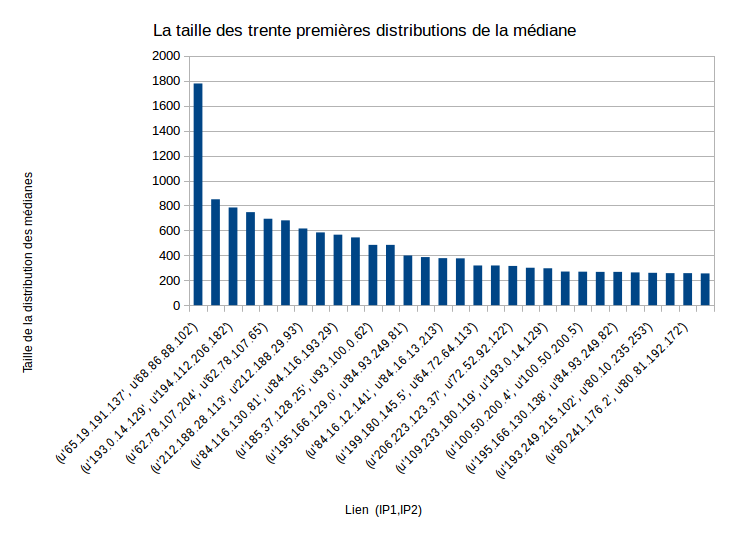
\includegraphics[width=1\linewidth]{illustrations/size_dist_med}
\caption{ La taille de la distribution des médianes des RTT différentiel }
\label{fig:size_dist_med}
\end{figure}


\subsection{Notes sur les traceroutes }

L'analyse menée sur les traceroutes collectées par les sondes Atlas n'utilise pas totalement les traceroutes sélectionnés suivant quand ils ont été capturés. 

\paragraph{Traceroute réussi ou échoué totalement.} Dans le travail de référence, les traceroutes sont stockés tels qu'ils sont, sans prétraitement à l'avance. Or un traceroute peut être éliminé à l'avance si ce dernier a échoué pour atteindre la destination prédéfinie. 


\paragraph{Traceroute réussi ou échoué partiellement.} Dans certains cas, la sonde Atlas ne parvient pas à atteindre un routeur intermédiaire durant son chemin vers la destination finale. Rappelons que pour un saut, l'implémentation du traceroute utilisée par les sondes Atlas envoie $3$ signaux par saut,  ainsi, on distingue deux cas : 
\begin{itemize}
	\item  la sonde ne reçoit aucune information sur les trois signaux;
	\item la sonde reçoit les informations de $1$ ou $2$ signaux.
\end{itemize}


\paragraph{Les adresses IP privées dans traceroute.} Dans la présente analyse, les adresses IP privées n'ont  aucune valeur ajoutée. Les liens à surveiller sont ceux visibles sur Internet, alors que les adresses IP privées reflètent la configuration des réseaux non publique.



\paragraph{L'utilité des attributs d'un enregistrement traceroute.} Une requête  traceroute est caractérisée par plusieurs attributs, plus de 40, décrits dans la figure \ref{fig:traceroute_attributes}. Les n\oe{}uds en gris sont de type liste, un élément de la liste est un objet formé les successeurs du n\oe{}ud en question. Les n\oe{}uds en vert sont les attributs utilisés par l'outil de détection des changements anormaux dans les délais d'un lien.


\begin{figure}[H]
\centering
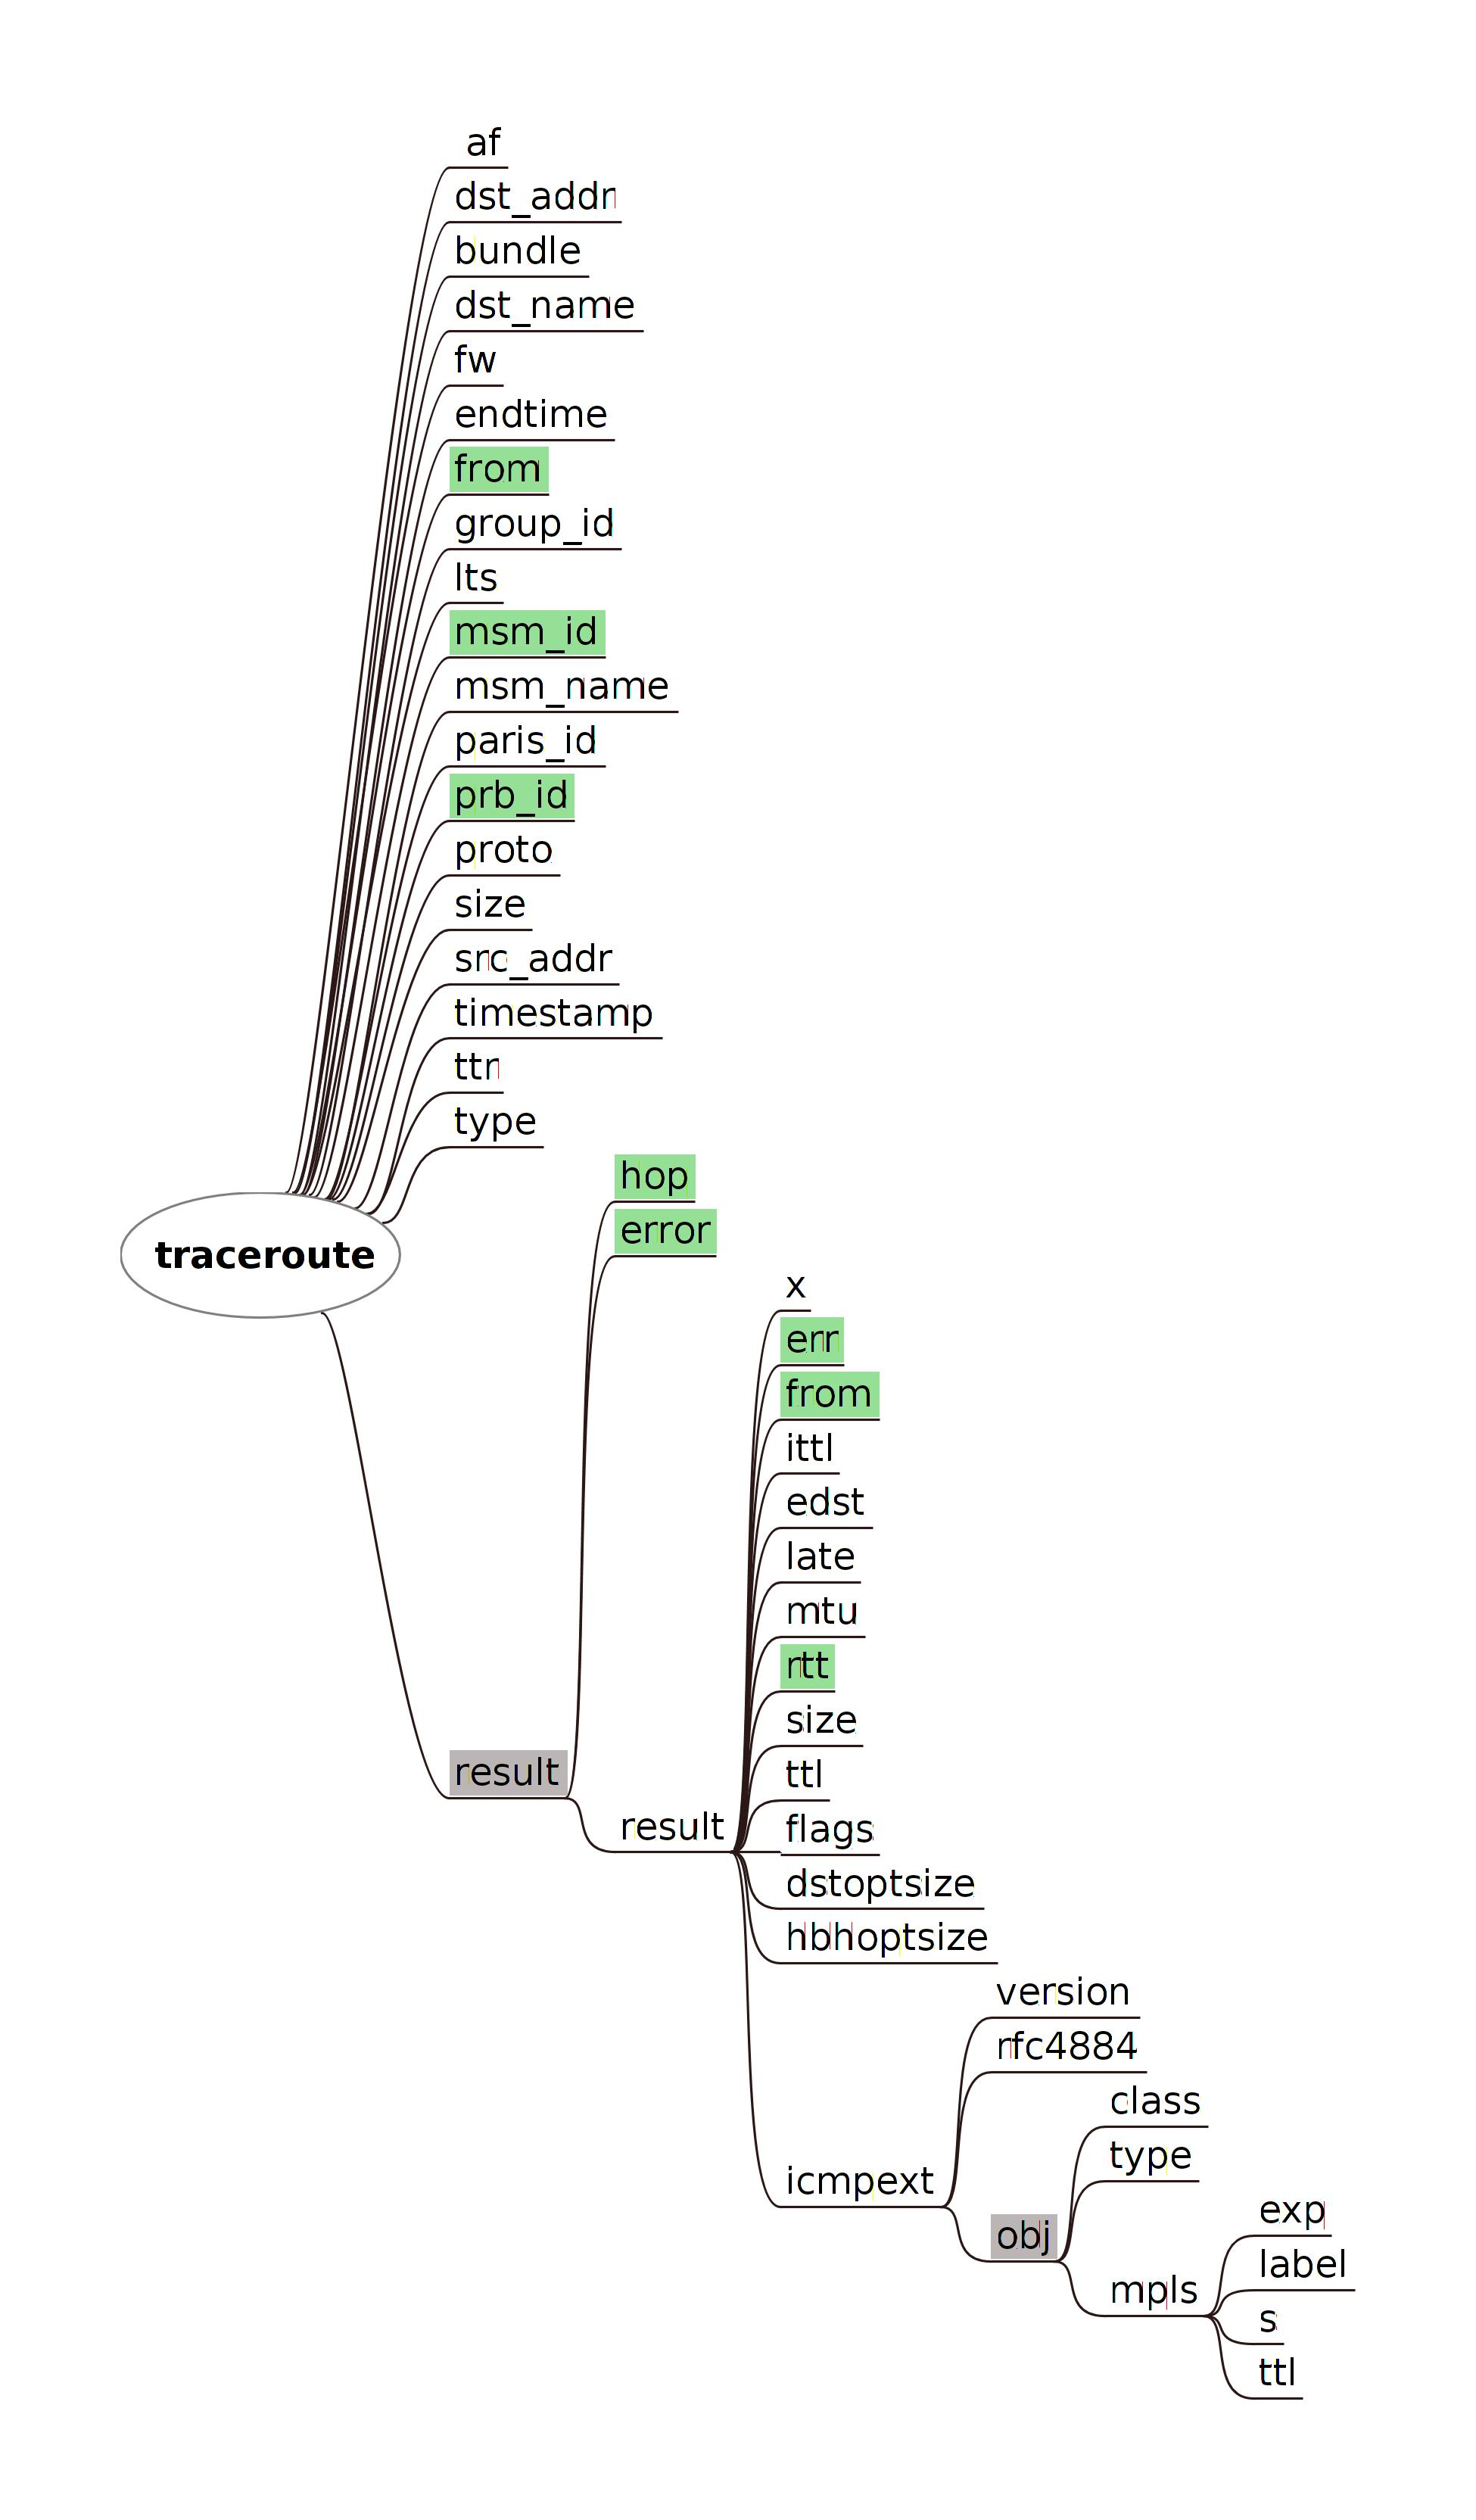
\includegraphics[width=0.7\linewidth]{illustrations/traceroute_attributes}
\caption{Les attributs possibles dans le résultat d'une requête traceroute}
\label{fig:traceroute_attributes}
\end{figure}


\newpage

\section{En pratique ...}

\paragraph{Le travail de référence}~

Le processus de l'analyse se fait en récupérant  d'abord les enregistrements des traceroutes depuis la base de données MongoDB. Ensuite, le traitement de chaque traceroute se poursuit dans la machine locale. Les résultats de type I, qui sont les changements des délais de tous les liens identifiés,   sont stockés localement dans la machine locale.
De plus, les détails de l'expérience sont aussi stockées dans MongoDB. Pour conclure toutes les opérations se déroulent dans la machine locale comme c'est illustré dans la figure \ref{fig:travail-de-reference}.

\begin{figure}[H]
\centering
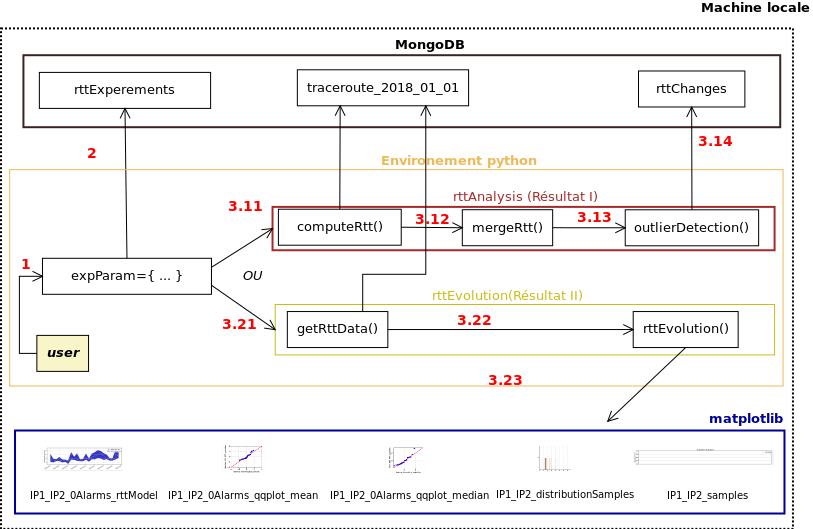
\includegraphics[width=1\linewidth]{illustrations/travail-de-reference}
\caption{Le processus d'analyse des traceroutes dans le travail de référence (MongoD)}
\label{fig:travail-de-reference}
\end{figure}

\paragraph{Intégration des AWS  Athena + S3 dans le travail de référence} \label{par:aws-stockage-seulement}~


La première adaptation du travail de référence en vue d'intégrer les services web d'Amazon est présentée dans la figure \ref{fig:travail-de-reference-avec-athena}. La différence par rapport à l'implémentation proposée dans le travail de référence est au niveau du stockage des données. En effet, au lieu de récupérer les traceroutes depuis les collections présentes dans MongoDB (traceroute\_2018\_01\_01), les traceroutes sont récupérés depuis  le service de stockage Amazon S3. Ces données ont été adaptées pour être utilisées par l'outil de la détection.

\begin{figure}[H]
\centering
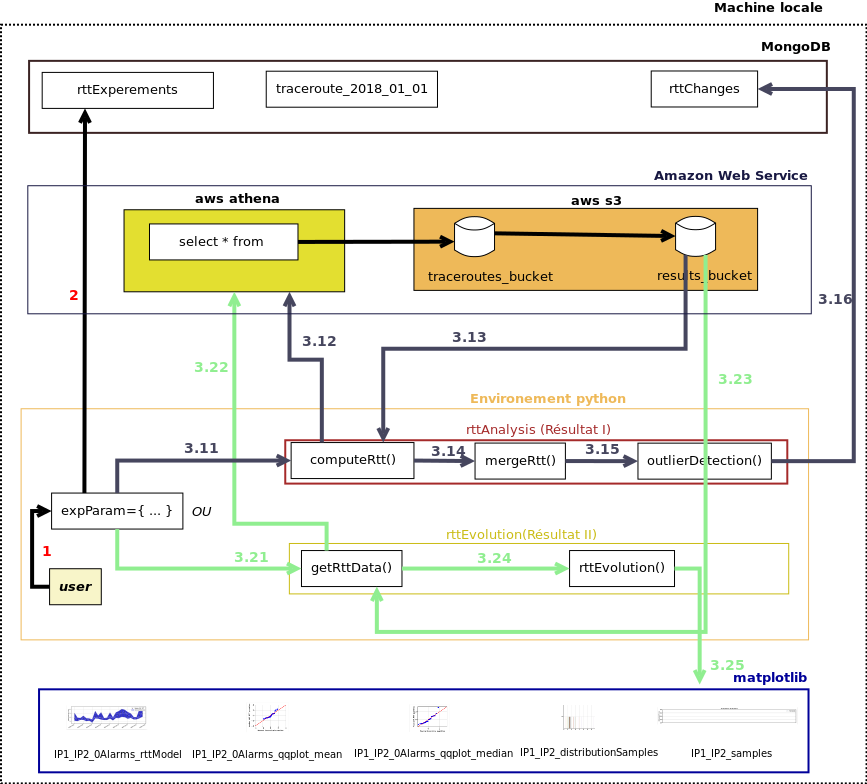
\includegraphics[width=1\linewidth]{illustrations/travail-de-reference-avec-athena}
\caption{Intégration des AWS  Athena + S3 dans le travail de référence}
\label{fig:travail-de-reference-avec-athena}
\end{figure}

\paragraph{Aller au delà du stockage sur Amazon S3}~

Les données manipulées par l'outil de la détection sont volumineuses, en plus du besoin du stockage, il faut aussi adopter les outils adéquats pour le traitement de ces données, ce qui n'était pas pris en considération dans l'adaptation décrite dans la section \ref{par:aws-stockage-seulement}.  

Et s'il existe une implémentation prenant en considération la manipulation des données massives en plus du stockage de ces dernières? On rappelle qu'une détection se déroule en récupérant d'abords les traceroutes de la période souhaitée, ensuite, chaque traceroute est analysé pour identifier les liens avec leur RTT différentiel (computeRTT()).Ces résultats sont fusionnés avec mergeRTT(). Enfin, la détection des anomalies se déclenche (outlierDetection()). Afin d'évaluer cette possibilité, on présente dans la figure \ref{fig:organigram-rttAnalysis} l'organigramme de la première étape dans la détection les changements des délais : computeRtt(). 

\begin{figure}[H]
\centering
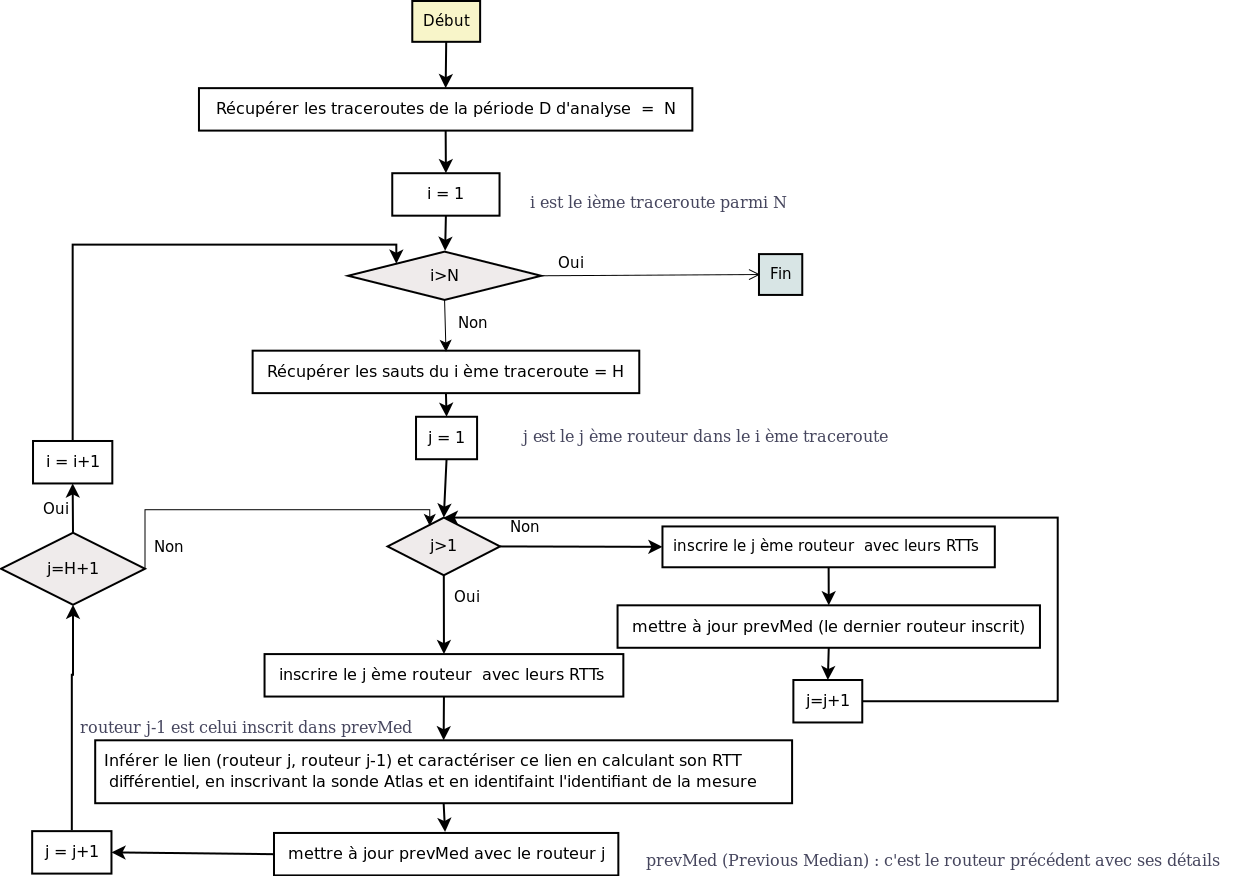
\includegraphics[width=1\linewidth]{illustrations/organigram-rttAnalysis}
\caption{ L'organigramme de  l'étape computeRTT()}
\label{fig:organigram-rttAnalysis}
\end{figure}

Soient les deux cas suivants :
\subparagraph{cas 1}

Supposant qu'il n'existe pas une requête SQL valide sur AWS Athena pour traiter tous les traceroutes en une seule fois, dans  ce cas, on doit créer une requête par traceroute. De plus, on doit créer un fichier résultat qui stocke les résultats à passer à l'étape mergeRTT(). En pratique, une heure comme période d'analyse a repris environ $ 18400 $ traceroutes. En effet, pour une heure, il faut lancer $ 18400 $ requêtes sur AWS Athena et $ 18400 $ opérations de lecture/écriture sur un fichier résultat si on souhaite le stocker dans AWS S3. Alors pour une semaine d'analyse? 


\subparagraph{cas 2}

Jusqu'à maintenant, avec la requête suivante \footnote{A faire évoluer si les services web d'Amazon qui seront utilisés dans la suite du mémoire.}:


\begin{figure}[H]
\centering
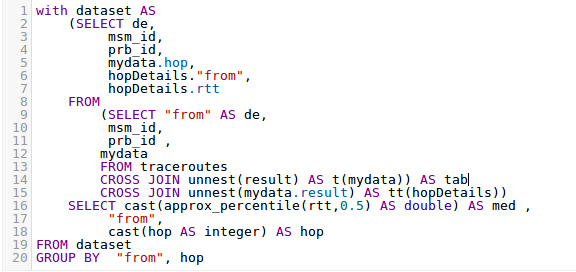
\includegraphics[width=1\linewidth]{illustrations/request}
\caption{Requête AWS Athena intermédiaire concernant le cas 2 }
\label{fig:request}
\end{figure}

Nous avons comme résultat :

\begin{figure}[H]
\centering
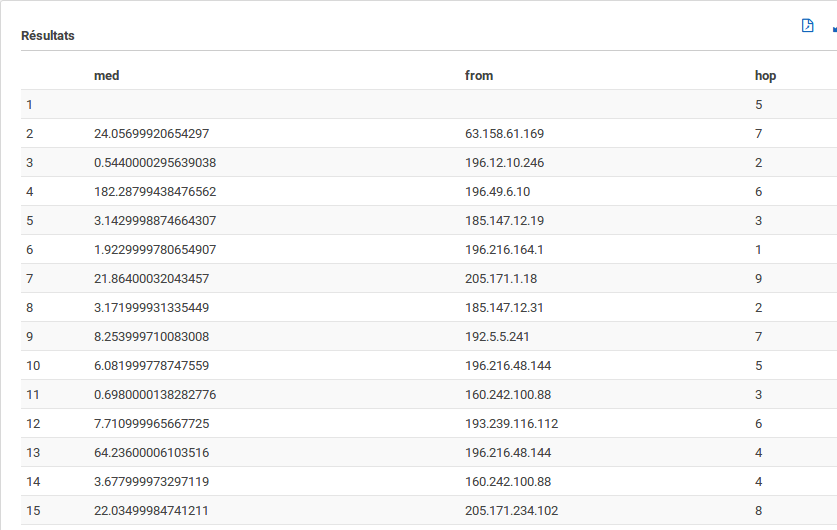
\includegraphics[width=1\linewidth]{illustrations/data_request}
\caption{Résultats de la requête AWS Athena intermédiaire concernant le cas 2}
\label{fig:data_request}
\end{figure}

Un lien est formé par l'adresse IP ayant avec \textit{hop} = i+1 et l'adresse IP ayant \textit{hop} = i. Le RTT différentiel est calculé en faisant la différence entre \textit{med} avec hop = i+1 et med avec hop = i, avec i   entier et doit concerner le même traceroute. Les résultats présentés dans \ref{fig:data_request} ne différencient pas les sauts du même traceroute.


Supposons qu'il existe une seule requête SQL valide sur AWS Athena et capable d'assurer toutes les opérations décrites dans l'organigramme \ref{fig:organigram-rttAnalysis} (y inclus l'inférence des liens), dans ce cas, il faut stocker les résultats intermédiaires pour qu'ils soient l'entrée de l'étape mergeRTT(). Et supposons aussi qu'il existe une requête SQL sur Athena capable de lire les résultats en question et d'appliquer la fusion entre les liens. Evaluons maintenant l'étape \textit{outlierDetection()}\footnote{Le principe de la détection est le même pour outlierDetection (résultat I) et rttEvolution (Résultats II)}. 


 On peut présenter  l'étape \textit{outlierDetection()} brièvement via l'organigramme  \ref{fig:outlier_detection_organigramm} :
 
 \begin{figure}[H]
\centering
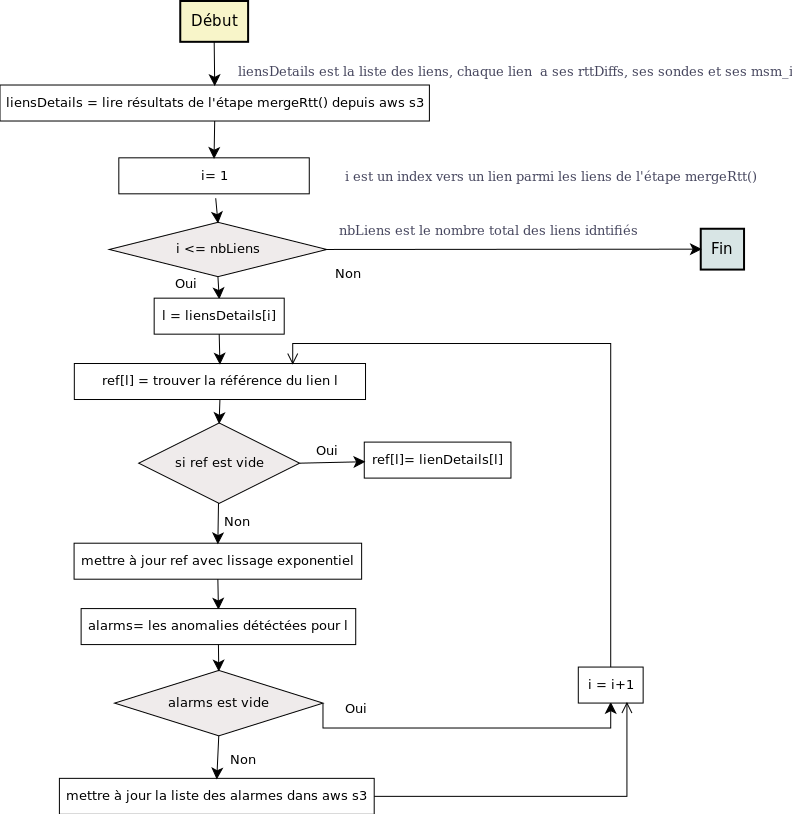
\includegraphics[width=1\linewidth]{illustrations/outlier_detection_organigramm}
\caption{L'organigramme de  l'étape outlierDetection()}
\label{fig:outlier_detection_organigramm}
\end{figure}

Ce qu'on peut noter à travers cet organigramme, c'est que l'évaluation de chaque lien $l$ nécessite l'accès en lecture aux résultats de l'étape mergeRtt()  d'une part et d'accéder à la référence de chaque lien  en lecture et écriture d'autre part. Si on suppose que les résultats intermédiaires sont stockés dans des fichiers disponibles sur AWS S3, est-il efficace de continuer l'analyse des traceroutes avec les deux service AWS Athena et S3?

En pratique si on considère l'analyse ayant les caractéristiques suivantes :
\begin{table}[H]
	\begin{tabular}{ll}
\textbf{Période} & entre 2015-10-20 00:00:00 et 2015-10-20 01:00:00\\ 
\textbf{Id de la mesure} &  $ 5004 $ \\
\textbf{Nb traceroutes} &  $ 17816 $\\
\textbf{Adressage IP} & $ 4 $ \\
\textbf{Nb de liens} &$ 26295 $\\
	\end{tabular}
	\caption{Récapitulatif d'une expérience de détection des anomalies }
	\label{tab:details-analyse}
\end{table}

Les données analysées sont disponibles sur GitHub\footnote{Source : \url{ https://github.com/hayatbellafkih/RipeAtlasTraceroutesAnalysis/blob/master/data/2015-10-20\%2000:00:00\_msmId5004.json.gz.}, consultée le $19/10/2018$. }. Le tableau 	\ref{tab:resultat-analyse} reprend $ 10 $ ($ 10/26295 $) liens issus de l'analyse décrite dans \ref{tab:details-analyse}. Ce sont les liens les plus rencontrés durant l'heure de l'analyse, autrement dit, ceux ayant la distribution la plus grande des RTTs différentiel.


\begin{table}[H]
	\centering
	\begin{tabular}{c c c}
	\textbf{Lien}	& \textbf{Nb RTT différentiel}& \textbf{Nb de sondes}\\
 ('192.5.5.241', '80.249.208.111') &	3737 &	3737 \\ \hline
 ('192.5.5.241', '80.81.194.57')  &	 1084 &	1084\\ \hline
 ('192.5.5.241', '216.200.0.10')  &	827 &	827\\ \hline
 ('216.200.0.10', '64.125.31.46')  &	802 &	802\\ \hline
 ('192.5.5.241', '80.249.208.140')  &	629 &	629\\ \hline
 ('195.219.194.46', '80.249.208.111')  &	443 &	443\\ \hline
 ('64.125.25.53', '64.125.31.46')  &	422 &	422\\ \hline
 ('192.5.5.241', '193.232.244.140')  &	420 &	420\\ \hline
 ('192.5.5.241', '193.239.116.112')  &	396 &	396\\ \hline
 ('64.125.20.250', '64.125.25.53') 	 &387 &	387\\ \hline
 ('192.5.5.241', '195.35.65.250')  &	371 &	371\\ \hline
 ('192.5.5.241', '193.232.246.140')  &	369	 &369\\ \hline
 ('192.5.5.241', '62.115.42.86')  &	360	 &360\\ \hline
 ('192.5.5.241', '206.223.119.2')  &	353	 &353\\ \hline
 ('192.5.5.241', '5.57.80.224')  &	353	 &353\\ \hline
	\end{tabular}
	\label{tab:resultat-analyse}
\end{table}

\paragraph{Conclusion}

Le service web d'Amazon Athena permet le mode lecture seulement des données, ainsi les tables créées ne peuvent pas être mises à jour, ce sont des tables utiles pour lire les données présentes sur AWS S3.  L'opération de la détection des anomalies des délais dans les liens passe par plusieurs étapes intermédiaires, de ce fait, il faut passer plusieurs opérations de lecture/écriture des résultats intermédiaires. En matière d'efficacité, on peut trouver mieux que les deux services d'Amazon  Athena et S3 pour ce projet en particulier.  En ce qui concerne la médiane, on a pas considéré l'efficacité de la fonction \textit{approx\_percentile(col, 0.5)} \footnote{Plus de détails sur \url{https://prestodb.io/docs/current/functions/aggregate.html}, consultée le $19/10/2018$.} en terme de précision, vu que le choix de ces deux services d'AWS n'est pas efficace pour l'opération de la détection.
 


\newpage
\section{L'algorithme de la détection des anomalies des délais d'un lien}

\subsection{Introduction}
Le suivi de l'évolution du RTT différentiel d'un lien (Résultat II) est effectué en deux grandes étapes : 
\begin{enumerate}
	\item La préparation des données (computeRTT(), MergeRttResults(), Prétraitement des résultats par timeWindow).
	\item L'évaluation des RTTs différentiels (rttEvolution()).
\end{enumerate}

Pour l'illustration, nous avons utilisé seulement deux traceroutes afin de montrer l'étape 1. Afin d'illustrer l'étape 2, nous avons choisi plusieurs\footnote{\url{ RipeAtlasTraceroutesAnalysis/data/traceroute_2018_01_01.json } et \url{ RipeAtlasTraceroutesAnalysis/data/traceroute_2018_01_02.json }} traceroutes pour les prérequis de l'algorithme de la détection. Les traceroutes ont été générés avec un script python. L'idée c'est de partir d'un traceroute et changer les RTTs du deuxième saut. Comme la détéction se déclenche à partir du 25 ème timeWindow, nous avons utilisé des RTTs avec des valeurs grandes afin d'assurer la détection d'une anomalie. 

Par exemple, tous les traceroutes du 01/01/2018 sont créés tel que :


\begin{lstlisting}
rtt1= [1, 2, 1, 3]
allrtts=[rtt1,rtt1,rtt1,rtt1,rtt1,rtt1,rtt1,rtt1,rtt1,rtt1,rtt1,rtt1,rtt1,rtt1,rtt1,rtt1,rtt1,rtt1,rtt1,rtt1,rtt1,rtt1,rtt1]
\end{lstlisting}

\begin{algorithm}[H]
	
	\begin{algorithmic}[1]

		\State $i   \leftrightarrow  1$
		\ForAll {$rtt \in allrtts$}
		
			\ForAll {$val \in rtt$}
		        \State tmptrace $ \leftrightarrow $ loadreferenceTraceroute()
		        
		                     \State   tmptrace["result"][1]['result'][0]['rtt'] $ \leftrightarrow $ tmptrace["result"][1]['result'][0]['rtt']+ val
		                     \State   tmptrace["result"][1]['result'][1]['rtt'] $ \leftrightarrow $ tmptrace["result"][1]['result'][1]['rtt']+ val
		                     \State   tmptrace["result"][1]['result'][2]['rtt'] $ \leftrightarrow $  tmptrace["result"][1]['result'][2]['rtt']+ val
		                    \State tmptrace["timestamp"]  $ \leftrightarrow $ tmptrace["timestamp"] + int(3600) * int(i)
	     	     \EndFor
	     	     \State i$ \leftrightarrow $ i+1
		
		\EndFor

	\end{algorithmic}
	\caption{}
	\label{algo:co}
\end{algorithm}


De la même manière nous avons généré les traceroutes concernant la journée 02/01/2018, avec :
\begin{lstlisting}
rtt1=[1, 2, 1, 3]
rtt11=[10680,10845,10998,10800]
rtt12=[1060,1045,1098,1080]
rtt13=[1060,1045,1098,1080]
allrtts=[rtt1,rtt1,rtt11,rtt12,rtt13,rtt1,rtt1,rtt1]
\end{lstlisting}


Dans la suite de cette section, nous allons travailler sur le graphique suivant :

\begin{figure}
\centering
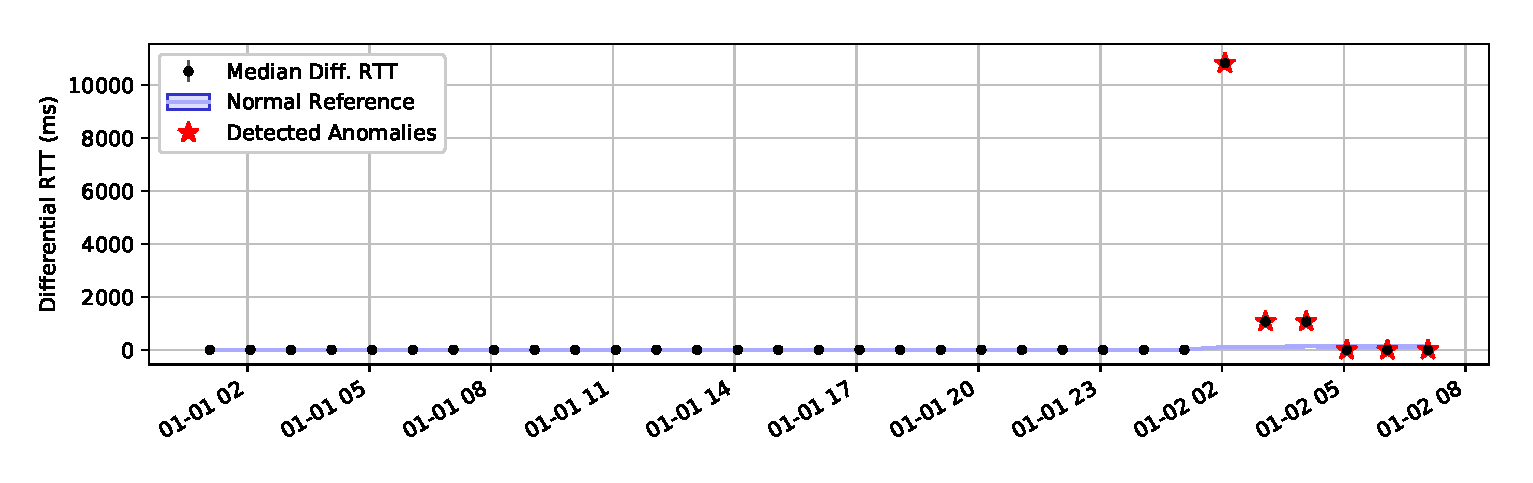
\includegraphics[width=1\linewidth]{illustrations/finalrttmodel}
\caption{L'évolution du RTT différentiel du lien 185\_147\_12\_31 - 89\_105\_200\_57}
\label{fig:finalrttmodel}
\end{figure}



 \subsection{Le fonctionnement de l'algorithme de la détection}
\paragraph{computeRTT()}~

\begin{algorithm}[H]
	
	\begin{algorithmic}[1]
		\Procedure{$start$, $end$}{}
		 \State $traceroutes$ $\leftrightarrow$ traceroutes capturés entre $start$ et $end$
		\ForAll {$currDate \in dates$}
		\State readOneTraceroute()
		\EndFor
		\EndProcedure
	\end{algorithmic}
	\caption{}
	\label{algo:computRTT}
\end{algorithm}

Le traitement d'un traceroute est détaillé si dessous, soit le premier traceroute dans timeWindow 2018-01-01 02:01:01:
\newpage
\begin{lstlisting}
{
	"lts":165,
	"msm_id":5004,
	"from":"89.105.202.4",
	"dst_name":"192.5.5.241",
	"proto":"UDP",
	"timestamp":1514773209,
	"fw":4790,
	"paris_id":9,
	"stored_timestamp":1514768539,
	"prb_id":4247,
	"af":4,
	"result":[
	{
		"result":[
		{
			"rtt":1.955,
			"size":28,
			"from":"89.105.200.57",
			"ttl":255
		},
		{
			"rtt":1.7,
			"size":28,
			"from":"89.105.200.57",
			"ttl":255
		},
		{
			"rtt":1.709,
			"size":28,
			"from":"89.105.200.57",
			"ttl":255
		}
		],
		"hop":1
	},
	{
		"result":[
		{
			"rtt":7.743,
			"size":28,
			"from":"185.147.12.31",
			"ttl":254
		},
		{
			"rtt":3.3030000000000004,
			"size":28,
			"from":"185.147.12.31",
			"ttl":254
		},
		{
			"rtt":3.3720000000000003,
			"size":28,
			"from":"185.147.12.31",
			"ttl":254
		}
		],
		"hop":2
	},
	{
		"result":[
		{
			"rtt":4.347,
			"size":28,
			"from":"185.147.12.19",
			"ttl":253
		},
		{
			"rtt":2.876,
			"size":28,
			"from":"185.147.12.19",
			"ttl":253
		},
		{
			"rtt":3.143,
			"size":28,
			"from":"185.147.12.19",
			"ttl":253
		}
		],
		"hop":3
	}
	],
	"dst_addr":"192.5.5.241",
	"src_addr":"89.105.202.4",
	"endtime":1514768403,
	"type":"traceroute",
	"msm_name":"Traceroute",
	"size":40
}

\end{lstlisting}

Le tableau suivant reprend chaque étape du traitement d'un traceroute:


\begin{landscape}
	
Itération 1 :
\begin{table}[H]
	\centering
	\begin{tabularx}{20cm}{|l|X|X|c|}
		\hline 
		\textbf{Hop} & \textbf{détails du signal}& \textbf{rttList}& \textbf{PrevMed}\\ \hline
 1 & \{'rtt': 1.955, 'from': '89.105.200.57'\} & \{'89.105.200.57': [1.955]\} & \{\} \\ \hline 
 1 & \{'rtt': 1.7, 'from': '89.105.200.57'\} & \{'89.105.200.57': [1.955, 1.7]\} & \{\} \\ \hline 
 1 & \{'rtt': 1.709, 'from': '89.105.200.57'\} & \{'89.105.200.57': [1.955, 1.7, 1.709]\} & \{\} \\ \hline 
	\end{tabularx}
\end{table}

\begin{table}[H]
	\centering
	\begin{tabularx}{20cm}{|l|X|X|c|X|}
		\hline 
		 \textbf{Routeur} & \textbf{dist} & \textbf{PrevMed}& \textbf{Med} & \textbf{rttMed} \\ \hline
89.105.200.57 & [1.955, 1.7, 1.709] & non & 1.709 &\{'89.105.200.57': 1.709\} \\ \hline
	\end{tabularx}
\end{table}
\end{landscape}

\begin{landscape}
Itération 2 :

\begin{table}[H]
	\centering

	\begin{tabularx}{20cm}{|c|X|X|X|}
		\hline 
		\textbf{Hop} & \textbf{détails du signal}& \textbf{rttList}& \textbf{PrevMed}\\ \hline
 2 & \{'rtt': 7.743, 'from': '185.147.12.31'\} & \{'185.147.12.31': [7.743]\} & \{'89.105.200.57': 1.709\} \\ \hline 
 2 & \{'rtt': 3.3030000000000004, 'from': '185.147.12.31'\} & \{'185.147.12.31': [7.743, 3.3030000000000004]\} & \{'89.105.200.57': 1.709\} \\ \hline 
 2 & \{'rtt': 3.3720000000000003, 'from': '185.147.12.31'\} & \{'185.147.12.31': [7.743, 3.3030000000000004, 3.3720000000000003]\} & \{'89.105.200.57': 1.709\} \\ \hline 

	\end{tabularx}
\end{table}
\begin{table}[H]
	\centering
	\resizebox{20cm}{!}{
	\begin{tabular}{|c|c|c|c|c|}
		\hline 
		\textbf{Routeur} & \textbf{dist} & \textbf{PrevMed}& \textbf{Med} & \textbf{rttMed} \\ \hline
185.147.12.31 & [7.743, 3.3030000000000004, 3.3720000000000003] & oui  & 3.3720000000000003 &\{'185.147.12.31': 3.3720000000000003\} \\ \hline
	\end{tabular}}
\end{table}
\begin{table}[H]
	\centering
	\resizebox{20cm}{!}{
		\begin{tabular}{|c|c|c|c|}
			\hline 
ip2 & ip1 & (ip1, ip2) in diffRtt & diffRtt[(ip1, ip2)] \\ \hline
185.147.12.31 & 89.105.200.57 &True& {'rtt': [1.7630000000000003], 'probe': ['89.105.202.4'], 'msmId':  {5004: [4247]}} \\ \hline

	\end{tabular}}
\end{table}
\begin{table}[H]
	\centering
	\resizebox{20cm}{!}{
		\begin{tabular}{|c|}
		diffRTT	\\ \hline
{('89.105.200.57', '185.147.12.31'): {'rtt': [1.6630000000000003], 'probe': ['89.105.202.4'], 'msmId':  {5004: set([4247])}}} \\ \hline
	\end{tabular}
	}
\end{table}

\begin{lstlisting}
>>> float(3.3720000000000003 ) - float(1.709)
1.6630000000000003 (est le RTT différentiel du lien ('89.105.200.57', '185.147.12.31') )

\end{lstlisting}
\end{landscape}


\begin{landscape}
	Itération 3 : 
	\begin{table}[H]
		\centering
		\resizebox{20cm}{!}{
	\begin{tabularx}{20cm}{|c|X|X|X|}
		\hline 
		\textbf{Hop} & \textbf{détails du signal}& \textbf{rttList}& \textbf{PrevMed}\\ \hline
		3 & \{'rtt': 4.347, 'from': u'185.147.12.19'\} & \{'185.147.12.19': [4.347]\} & \{'185.147.12.31': 3.3720000000000003\} \\ \hline	 
		3 & \{'rtt': 2.876, 'from': u'185.147.12.19'\} & \{'185.147.12.19': [4.347, 2.876]\} & \{'185.147.12.31': 3.3720000000000003\} \\ \hline  
		3 & \{'rtt': 3.143, 'from': u'185.147.12.19'\} & \{'185.147.12.19': [4.347, 2.876, 3.143]\} & \{'185.147.12.31': 3.3720000000000003\}  \\ \hline
	\end{tabularx}
}
\end{table}

\begin{table}[H]
	\centering
	\resizebox{20cm}{!}{
		\begin{tabular}{|c|c|c|c|c|}
			\hline 
			\textbf{Routeur} & \textbf{dist} & \textbf{PrevMed}& \textbf{Med} & \textbf{rttMed} \\ \hline
			
			185.147.12.19 & [4.347, 2.876, 3.143] & 1  & 3.143 &{'185.147.12.19': 3.143} 
			
			
			\\ \hline
		\end{tabular}}
	\end{table}
	
		\begin{table}[H]
			\centering
			\resizebox{20cm}{!}{
				\begin{tabular}{|c|c|c|c|}
					\hline 
					ip2 & ip1 & (ip1, ip2) in diffRtt & diffRtt[(ip1, ip2)] \\ \hline
					185.147.12.19 & 185.147.12.31 &True& {'rtt': [-0.22900000000000054], 'probe': ['89.105.202.4'], 'msmId':  {5004: set([4247])}} 
					\\ \hline
					
				\end{tabular}}
			\end{table}
			
\begin{lstlisting}
>>>  float(3.143) - float(3.3720000000000003)
-0.22900000000000054 (est le RTT différentiel du lien ('185.147.12.31', '185.147.12.19') )
\end{lstlisting}
			
			\begin{table}[H]
				\centering
				\resizebox{20cm}{!}{
					\begin{tabular}{|c|}
						\hline
						\textbf{diffRTT}	\\ \hline
						\{('89.105.200.57', '185.147.12.31'): \{'rtt': [1.6630000000000003], 'probe': ['89.105.202.4'], 'msmId':  \{5004: set([4247])\}\},  \\
						('185.147.12.31', '185.147.12.19'): \{'rtt': [-0.22900000000000054], 'probe': ['89.105.202.4'], 'msmId': \{5004: set([4247])\}\}\}
						\\ \hline
					\end{tabular}
				}
			\end{table}
				\end{landscape}
\newpage

A l'issue du traitement du premier traceroute, deux liens ont été identifiés, chacun est décrit par son RTT différentiel, les sondes Atlas ayant identifié ce lien et enfin les mesures lancées par les sondes Atlas ayant impliqué ce lien.  

Soit le deuxième traceroute dans timeWindow 2018-01-01 02:01:01:
\begin{lstlisting}
{
	"lts":165,
	"msm_id":5004,
	"from":"89.105.202.4",
	"dst_name":"192.5.5.241",
	"proto":"UDP",
	"timestamp":1514773210,
	"fw":4790,
	"paris_id":9,
	"stored_timestamp":1514768539,
	"prb_id":4247,
	"af":4,
	"result":[
	{
		"result":[
		{
			"rtt":1.955,
			"size":28,
			"from":"89.105.200.57",
			"ttl":255
		},
		{
			"rtt":1.7,
			"size":28,
			"from":"89.105.200.57",
			"ttl":255
		},
		{
			"rtt":1.709,
			"size":28,
			"from":"89.105.200.57",
			"ttl":255
		}
		],
		"hop":1
	},
	{
		"result":[
		{
			"rtt":4.347,
			"size":28,
			"from":"185.147.12.19",
			"ttl":253
		},
		{
			"rtt":2.876,
			"size":28,
			"from":"185.147.12.19",
			"ttl":253
		},
		{
			"rtt":3.143,
			"size":28,
			"from":"185.147.12.19",
			"ttl":253
		}
		],
		"hop":2
	},
	{
		"result":[
		{
			"rtt":7.843,
			"size":28,
			"from":"185.147.12.31",
			"ttl":254
		},
		{
			"rtt":6.4,
			"size":28,
			"from":"185.147.12.31",
			"ttl":254
		},
		{
			"rtt":7,
			"size":28,
			"from":"185.147.12.31",
			"ttl":254
		}
		],
		"hop":3
	}
	],
	"dst_addr":"192.5.5.241",
	"src_addr":"89.105.202.4",
	"endtime":1514768403,
	"type":"traceroute",
	"msm_name":"Traceroute",
	"size":40
}
\end{lstlisting}

Nous allons procéder aux même itérations faites pour le premier traceroute. 


\begin{landscape}
	Itération 1 : 
	\begin{table}[H]
		\centering
		\resizebox{20cm}{!}{
			\begin{tabularx}{20cm}{|c|X|X|X|}
				\hline 
				\textbf{Hop} & \textbf{détails du signal}& \textbf{rttList}& \textbf{PrevMed}\\ \hline
				 1 & \{'rtt': 1.955, 'from': '89.105.200.57'\} & \{'89.105.200.57': [1.955]\} & \{\} \\ \hline
				 1 & \{'rtt': 1.7, 'from': '89.105.200.57'\} & \{'89.105.200.57': [1.955, 1.7]\} & \{\} \\ \hline
				 1 & \{'rtt': 1.709, 'from': '89.105.200.57'\} & \{'89.105.200.57': [1.955, 1.7, 1.709]\} & \{\} \\ \hline
			\end{tabularx}
		}
	\end{table}
	
	\begin{table}[H]
		\centering
		\resizebox{20cm}{!}{
			\begin{tabular}{|c|c|c|c|c|}
				\hline 
				\textbf{Routeur} & \textbf{dist} & \textbf{PrevMed}& \textbf{Med} & \textbf{rttMed} \\ \hline
				89.105.200.57 & [1.955, 1.7, 1.709] & 0  & 1.709 &{'89.105.200.57': 1.709} 
				
				\\ \hline
			\end{tabular}}
		\end{table}
		
		
				\begin{table}[H]
					\centering
					\resizebox{20cm}{!}{
						\begin{tabular}{|c|}
							\hline
							diffRTT	\\ \hline
			\{('89.105.200.57', '185.147.12.31'): \{'rtt': [1.6630000000000003], 'probe': [u'89.105.202.4'], 'msmId':  \{5004: set([4247])\}\}, \\
			('185.147.12.31', '185.147.12.19'): \{'rtt': [-0.22900000000000054], 'probe': ['89.105.202.4'], 'msmId':  \{5004: set([4247])\}\}\}\\ \hline
						\end{tabular}
					}
				\end{table}
		\end{landscape}
		
		
		\begin{landscape}
			Itération  2: 
			\begin{table}[H]
				\centering
				\resizebox{20cm}{!}{
					\begin{tabularx}{20cm}{|c|X|X|X|}
						\hline 
						\textbf{Hop} & \textbf{détails du signal}& \textbf{rttList}& \textbf{PrevMed}\\ \hline
						 2 & \{'rtt': 4.347, 'from': '185.147.12.19'\} & \{'185.147.12.19': [4.347]\} & \{'89.105.200.57': 1.709\} \\ \hline 
						 2 & \{'rtt': 2.876, 'from': '185.147.12.19'\} & \{'185.147.12.19': [4.347, 2.876]\} & \{'89.105.200.57': 1.709\} \\ \hline 
						 2 & \{'rtt': 3.143, 'from': '185.147.12.19'\} & \{'185.147.12.19': [4.347, 2.876, 3.143]\} & \{'89.105.200.57': 1.709\} \\ \hline
					\end{tabularx}
				}
			\end{table}


			\begin{table}[H]
				\centering
				\resizebox{20cm}{!}{
					\begin{tabular}{|c|c|c|c|c|}
						\hline 
						\textbf{Routeur} & \textbf{dist} & \textbf{PrevMed}& \textbf{Med} & \textbf{rttMed} \\ \hline
					185.147.12.19 & [4.347, 2.876, 3.143] & 1  & 3.143 &\{'185.147.12.19': 3.143\} 
						\\ \hline
					\end{tabular}}
				\end{table}
				
				\begin{table}[H]
					\centering
					\resizebox{20cm}{!}{
						\begin{tabular}{|c|c|c|c|}
							\hline 
							ip2 & ip1 & (ip1, ip2) in diffRtt & diffRtt[(ip1, ip2)] \\ \hline
185.147.12.19 & 89.105.200.57 &True &\{'rtt': [1.4339999999999997], 'probe': ['89.105.202.4'], 'msmId':  \{5004: set([4247])\}\} 
							\\ \hline
							
						\end{tabular}}
					\end{table}
					
\begin{lstlisting}
>>> float(3.143) - float(1.709) = 1.4339999999999997
\end{lstlisting}
					
\begin{table}[H]
	\centering
	\resizebox{20cm}{!}{
		\begin{tabular}{|c|}
			\hline
			\textbf{diffRTT}	\\ \hline
	\{('89.105.200.57', '185.147.12.19'): \{'rtt': [1.4339999999999997], 'probe': ['89.105.202.4'], 'msmId':  \{5004: set([4247])\})\},\\ ('89.105.200.57', '185.147.12.31'): \{'rtt': [1.6630000000000003], 'probe': ['89.105.202.4'], 'msmId':  \{5004: set([4247])\}\},\\ ('185.147.12.31', '185.147.12.19'): \{'rtt': [-0.22900000000000054], 'probe': ['89.105.202.4'], 'msmId':  \{5004: set([4247])\}\}\}
	\\ \hline
		\end{tabular}
	}
\end{table}
				\end{landscape}
				
				
\begin{landscape}
	Itération 3 : 
	\begin{table}[H]
		\centering
		\resizebox{20cm}{!}{
			\begin{tabularx}{20cm}{|c|X|X|X|}
				\hline 
				\textbf{Hop} & \textbf{détails du signal}& \textbf{rttList}& \textbf{PrevMed}\\ \hline
 3 & \{'rtt': 7.843, 'from': '185.147.12.31'\} & \{'185.147.12.31': [7.843]\} & \{'185.147.12.19': 3.143\} \\ \hline  
 3 & \{'rtt': 6.4, 'from': '185.147.12.31'\} & \{'185.147.12.31': [7.843, 6.4]\} & \{'185.147.12.19': 3.143\} \\ \hline  
 3 & \{'rtt': 7, 'from': '185.147.12.31'\} & \{'185.147.12.31': [7.843, 6.4, 7]\} & \{'185.147.12.19': 3.143\} \\ \hline
			\end{tabularx}
		}
	\end{table}
	
	\begin{table}[H]
		\centering
		\resizebox{20cm}{!}{
			\begin{tabular}{|c|c|c|c|c|}
				\hline 
				\textbf{Routeur} & \textbf{dist} & \textbf{PrevMed}& \textbf{Med} & \textbf{rttMed} \\ \hline
				185.147.12.31 & [7.843, 6.4, 7] & 1  & 7.0 &{'185.147.12.31': 7.0} 
	 
				\\ \hline
			\end{tabular}}
		\end{table}
		
		\begin{table}[H]
			\centering
			\resizebox{20cm}{!}{
				\begin{tabular}{|c|c|c|c|}
					\hline 
					ip2 & ip1 & (ip1, ip2) in diffRtt & diffRtt[(ip1, ip2)] \\ \hline
					185.147.12.31 & 185.147.12.19 &True& \{'rtt': [3.857], 'probe': ['89.105.202.4'], 'msmId':\{5004: set([4247])\}\} 
					\\ \hline
					
				\end{tabular}}
			\end{table}
				
			\begin{table}[H]
				\centering
				\resizebox{20cm}{!}{
					\begin{tabular}{|l|}
						\hline
						\textbf{diffRTT}	\\ \hline
\{('89.105.200.57', '185.147.12.19'): \{'rtt': [1.4339999999999997], 'probe': ['89.105.202.4'], 'msmId':  \{5004: set([4247]\})\},\\ ('89.105.200.57', '185.147.12.31'): \{'rtt': [1.6630000000000003], 'probe': ['89.105.202.4'], 'msmId':  \{5004: set([4247])\}\}, \\
('185.147.12.31', '185.147.12.19'): \{'rtt': [-0.22900000000000054], 'probe': ['89.105.202.4'], 'msmId':  \{5004: set([4247])\}\},\\ ('185.147.12.19', '185.147.12.31'): \{'rtt': [3.857], 'probe': ['89.105.202.4'], 'msmId': \{5004: set([4247])\}\}\} 
						
						\\ \hline
					\end{tabular}
				}
			\end{table}
		\end{landscape}

\paragraph{MergeRttResults()}~

On constate que les deux routeurs '185.147.12.19' et '185.147.12.31' sont impliqués dans deux liens  mais l'ordre est différent. Dans le travail de référence, les liens ('185.147.12.19', '185.147.12.31') et ('185.147.12.31','185.147.12.19')sont similaires en terme du RTT différentiel qui les caractérisent. De ce fait, une fois tous les traceroutes sont analysés d'un timeWindow, une fusion est appliquée. 
La fusion s'applique sur les RTTs différentiel, les sondes Atlas et les identifiants des mesures.  Par exemple, les deux traceroutes analysés ci-dessus ont impliqué un même lien, la fusion des informations sur les deux liens donne le résultat dans le tableau \ref{tab:aftermerge}.


	\begin{landscape}
		
		Avant :
					\begin{table}[H]
						\centering
						\resizebox{20cm}{!}{
							\begin{tabular}{|l|}
								\hline
								\textbf{diffRTT}	\\ \hline
								\{('89.105.200.57', '185.147.12.19'): \{'rtt': [1.4339999999999997], 'probe': ['89.105.202.4'], 'msmId':  \{5004: set([4247]\})\},\\ ('89.105.200.57', '185.147.12.31'): \{'rtt': [1.6630000000000003], 'probe': ['89.105.202.4'], 'msmId':  \{5004: set([4247])\}\}, \\
								('185.147.12.31', '185.147.12.19'): \{'rtt': [-0.22900000000000054], 'probe': ['89.105.202.4'], 'msmId':  \{5004: set([4247])\}\},\\ ('185.147.12.19', '185.147.12.31'): \{'rtt': [3.857], 'probe': ['89.105.202.4'], 'msmId': \{5004: set([4247])\}\}\} 
								
								\\ \hline
							\end{tabular}
						}
					\end{table}
		Après: 
	
	
		
		\begin{table}[H]
			\centering
			\resizebox{20cm}{!}{
				\begin{tabular}{|l|}
					\hline
					\textbf{diffRTT}	\\ \hline
					
					\{('185.147.12.19', '185.147.12.31'): \{'rtt': [-0.22900000000000054, 3.857], 'probe': ['89.105.202.4', '89.105.202.4'], 'msmId':  \{5004: set([4247])\}\},\\
					
					('185.147.12.31', '89.105.200.57'): \{'rtt': [1.6630000000000003], 'probe': ['89.105.202.4'], 'msmId': \{5004: set([4247])\}\},\\
					
					('185.147.12.19', '89.105.200.57'): \{'rtt': [1.4339999999999997], 'probe': ['89.105.202.4'], 'msmId': \{5004: set([4247])\}\}\}
					\\ \hline
				\end{tabular}
			}
				\caption{After Merge}
				\label{tab:aftermerge}
		\end{table}
		\end{landscape}
		
\paragraph{Prétraitement des résultats par timeWindow}~

Le suivi de l'évolution du délai du lien dépend de son RTT différentiel. Ce suivi est fait par timeWindow. Après avoir traiter tous les traceroutes, et avoir un diffRTT par timeWindow, on procède une sorte de normalisation. Les dates appartenant à un même timeWindow sont représentées par une seule date appartenant au timewindow.


\begin{landscape}

		\begin{table}[H]
			\centering
			\resizebox{20cm}{!}{
				\begin{tabular}{|c|c|}
					\hline
\textbf{diffRTT}	 & \textbf{timestamps} \\ \hline
('89.105.200.57', '185.147.12.19'): \{'rtt': [1.4339999999999997], 'probe': ['89.105.202.4'], 'msmId':  \{5004: set([4247])\}\}& 1514773210 \\\hline

('89.105.200.57', '185.147.12.31'): \{'rtt': [1.6630000000000003], 'probe': ['89.105.202.4'], 'msmId':  \{5004: set([4247])\}\} & 1514773209\\\hline
('185.147.12.31', '185.147.12.19'): \{'rtt': [-0.22900000000000054], 'probe': ['89.105.202.4'], 'msmId':  \{5004: set([4247])\})\}&1514773209\\\hline
('185.147.12.19', '185.147.12.31'): \{'rtt': [3.857], 'probe': ['89.105.202.4'], 'msmId':  \{5004: set([4247])\}\}\} & 1514773210\\\hline
					
				\end{tabular}
			}
		\end{table}
		
		Avec : \textbf{1514773210} = 01/01/2018 02:20:10  et \textbf{1514773209} = 01/01/2018 02:20:09.
		
		
				\begin{table}[H]
					\centering
					\resizebox{20cm}{!}{
						\begin{tabular}{|l|}
							\hline
							\textbf{diffRTT}	\\ \hline
							
							\{('185.147.12.19', '185.147.12.31'): \{'rtt': [-0.22900000000000054, 3.857], 'probe': ['89.105.202.4', '89.105.202.4'], 'msmId':  \{5004: set([4247])\}\},\\
							
							('185.147.12.31', '89.105.200.57'): \{'rtt': [1.6630000000000003], 'probe': ['89.105.202.4'], 'msmId': \{5004: set([4247])\}\},\\
							
							('185.147.12.19', '89.105.200.57'): \{'rtt': [1.4339999999999997], 'probe': ['89.105.202.4'], 'msmId': \{5004: set([4247])\}\}\}
							\\ \hline
						\end{tabular}
					}
					\caption{After Merge}
					\label{tab:aftermergee}
				\end{table}
				
						\begin{table}[H]
							\centering
							\resizebox{20cm}{!}{
								\begin{tabular}{|c|c|c|}
									\hline
									(ip1, ip2) &rtts & date	\\ \hline
('185.147.12.19', '185.147.12.31') & [-0.22900000000000054, 3.857]&


 [datetime.datetime(2018, 1, 1, 2, 1, 1), datetime.datetime(2018, 1, 1, 2, 1, 1)] \\

('185.147.12.31', '89.105.200.57')& [1.6630000000000003]& [datetime.datetime(2018, 1, 1, 2, 1, 1)] \\
 ('185.147.12.19', '89.105.200.57')& [1.4339999999999997]& [datetime.datetime(2018, 1, 1, 2, 1, 1)]\\ \hline
										
								\end{tabular}
							}
						\end{table}
Pourquoi datetime.datetime(2018, 1, 1, 2, 1, 1) et pas datetime.datetime(2018, 1, 1, 2, 20, 09) ? 
La date de début est 01/01/2018 01:01:01, cette date est convertie en UTC (+1 heure), ainsi le premier timeWindow est 01/01/2018 02:01:01, le suivant est 01/01/2018 03:01:01, etc.

A ce stade, les données brutes sont prêtes passer à la détection des changements dans les délais. Les sorties des étapes décrites ci-dessus sont deux informations \textit{rawDiffRtt} et \textit{rawDates}. Pour chaque lien, on trouve les informations correspondantes à la fois dans \textit{rawDiffRtt} et \textit{rawDates}. Pour l'exemple précédent:

\begin{lstlisting}[language=Python]
('rawDiffRtt ': defaultdict(<type 'list'>, {
(u'185.147.12.19', u'185.147.12.31'): [-0.22900000000000054, 3.857], (u'185.147.12.31', u'89.105.200.57'): [1.6630000000000003], (u'185.147.12.19', u'89.105.200.57'): [1.4339999999999997]}))
('rawDates ': defaultdict(<type 'list'>, 
{(u'185.147.12.19', u'185.147.12.31'): [datetime.datetime(2018, 1, 1, 2, 1, 1), datetime.datetime(2018, 1, 1, 2, 1, 1)], 
(u'185.147.12.31', u'89.105.200.57'): [datetime.datetime(2018, 1, 1, 2, 1, 1)], 
(u'185.147.12.19', u'89.105.200.57'): [datetime.datetime(2018, 1, 1, 2, 1, 1)]}))
\end{lstlisting}
\end{landscape}

\paragraph{rttEvolution()}~

Afin d'illustrer la procédure de la détection des anomalies, il faut produire comme données d'entrée au minimum $96$ traceroutes. Afin de procéder la détection, il faut avoir minimum $4$ RTTs différentiels par timeWindow. De plus, la vérification des deux intervalles de confiance se déclenche à partir de la 25 ème timeWindow. Ce que nécessite au minimum $96$ traceroutes afin de passer au moins une fois par toute les étapes de la détection. 

 Comme paramètres de l'analyse on note:
 
 \begin{table}
\begin{tabular}{ll}
	 Date de début &\\
	 Date de fin & Tuesday 2 January 2018 10:14:22\\
	 TimeWindow (secondes) & 3600 \\ 
	 Préfixes & None \\
	 Lien & ('185.147.12.31', '89.105.200.57')\\
 \end{tabular}
 \end{table}
 
 Pour chaque timeWindow $d$ les opérations suivantes sont effectuées:
 
 \begin{enumerate}
 	\item Calcul de la médiane des RTTs différentiels de la distribution (dist) caractérisant le lien durant $d$ (\textit{median}).
 	
 	\item Calcul de la moyenne des RTTs différentiels de la distribution caractérisant le lien durant $d$ (\textit{mean}).
 	
 	\item Calcul du score de wilson \textit{wilsonCi}: wilsonCi[0] et wilsonCi[1].
 	
\begin{lstlisting}
  wilsonCi = sm.stats.proportion_confint(len(dist)/2, len(dist), 0.05, "wilson")
  wilsonCi = np.array(wilsonCi)*len(dist)
\end{lstlisting}
 	
 	\item Calcul de l'intervalle de confiance \textit{ciLow} et \textit{ciHight} à partir du \textit{wilsonCi}.
 	
\begin{lstlisting}
ciLow.append( median[-1] - dist[int(wilsonCi[0])] )
ciHigh.append( dist[int(wilsonCi[1])] - median[-1] )
\end{lstlisting}
 	\item Mise à jour l'intervalle de confiance de référence (\textit{smoothAvg}, \textit{smoothHi} et \textit{smoothLow}).
 	
 	\item  Comparaison de l'intervalle de confiance calculé pour $d$  avec le dernier intervalle de référence. 
 	
 	Tant que le nombre des timewindows analysés ne dépassent pas $ 24 $, aucune comparaison ne sera prévue, c'est à partir du $25$ ème timeWindow que la comparaison se fait.
 	
 	
 	Pour précision, les détails des timeWindows qui précèdent $d$ sont conservés, toutefois la comparaison est faite avec le  dernier intervalle de confiance de référence. Ce dernier inclut l'historique du lien en terme des RTTs différentiels.
 	
 	
 \end{enumerate}
 
 Les étapes $ 5 $ et $ 6 $ peuvent être illustrées avec le code source suivant:
 
  \begin{lstlisting}[language=python,numbers=left,
  frame=single,
  showstringspaces=true,
  basicstyle=\footnotesize,
  keywordstyle=\color{blue}\ttfamily\textbf,
  identifierstyle=\color{magenta}\ttfamily,
  stringstyle=\color{red}\ttfamily,
  commentstyle=\color{cyan}\ttfamily\textit
  ]
		#Mise à jour de l'intervalle de confiance de référence
        if len(smoothAvg)<24:
	        smoothAvg.append(median[-1])
	        smoothHi.append(dist[int(wilsonCi[1])])
	        smoothLow.append(dist[int(wilsonCi[0])])
        elif len(smoothAvg)==24:
	        smoothAvg.append(np.median(smoothAvg))
	        smoothHi.append(np.median(smoothHi))
	        smoothLow.append(np.median(smoothLow))
	        for i in range(24):
		        smoothAvg[i] = smoothAvg[-1]
		        smoothHi[i] = smoothHi[-1]
		        smoothLow[i] = smoothLow[-1]
        else:
	        #Lissage exponentiel
	        smoothAvg.append(0.99*smoothAvg[-1]+0.01*median[-1])
	        smoothHi.append(0.99*smoothHi[-1]+0.01*dist[int(wilsonCi[1])])
	        smoothLow.append(0.99*smoothLow[-1]+0.01*dist[int(wilsonCi[0])])
        
        #La comparaison entre les intervalles de confiance 
        if (median[-1]-ciLow[-1] > smoothHi[-1] or median[-1]+ciHigh[-1] < smoothLow[-1]) and np.abs(median[-1]-smoothAvg[-1])>1:
	        alarmsDates.append(d)
	        alarmsValues.append(median[-1])
 
 \end{lstlisting}
 
 Les tableaux ci-dessous illustrent les différentes  itérations de la détection. 

\begin{table}[H]
	\centering
	
		\resizebox{6cm}{!}{
				\rowcolors{1}{ligntrose}{lightgray}
 \begin{tabular}{ll}
 		\textbf{Itération}& 1\\
 \textbf{timeWindow}	 &  01/01/2018 01:04:21 \\
 \textbf{median} & [2.9630000000000005]\\ 
 \textbf{mean} &  [3.2130000000000005]\\
 \textbf{ciLow} & [0.5] \\
 \textbf{ciHigh}& [1.5000000000000004]\\
 \textbf{smoothAvg} &[2.9630000000000005] \\
  \textbf{smoothHi} & [4.463000000000001]\\
  \textbf{smoothLow} &[2.4630000000000005]\\ 
  \end{tabular} }
\end{table}
\begin{table}[H]
	\centering
		\resizebox{8cm}{!}{
	\rowcolors{1}{ligntrose}{lightgray}
			\begin{tabular}{ll}
				\textbf{Itération}& 2\\
				\textbf{timeWindow} &01/01/2018 02:04:21\\ 
				\textbf{median} &[2.9630000000000005, 2.9630000000000005]\\ \textbf{mean}&[3.2130000000000005, 3.2130000000000005]\\  \textbf{ciLow}&[0.5, 0.5] \\
				\textbf{ciHigh}  &[1.5000000000000004, 1.5000000000000004]\\  \textbf{smoothAvg}&[2.9630000000000005, 2.9630000000000005] \\ 
					\textbf{smoothHi}&[4.463000000000001, 4.463000000000001]\\
					\textbf{smoothLow}  &[2.4630000000000005, 2.4630000000000005]\\
					
				\end{tabular} 
			}
\end{table}

 \begin{table}[H]
 	\centering
 	\resizebox{\textwidth}{!}{
 			\rowcolors{1}{ligntrose}{lightgray}
 		\begin{tabular}{ll}
 			\textbf{Itération}& 3\\
 			\textbf{timeWindow}	 &   01/01/2018 03:04:21   \\
 			\textbf{median} & [2.9630000000000005, 2.9630000000000005, 2.9630000000000005]\\ 
 			\textbf{mean} & [3.2130000000000005, 3.2130000000000005, 3.2130000000000005]  \\
 			\textbf{ciLow} & [0.5, 0.5, 0.5] \\
 			\textbf{ciHigh}& [1.5000000000000004, 1.5000000000000004, 1.5000000000000004]\\
 			\textbf{smoothAvg} & [2.9630000000000005, 2.9630000000000005, 2.9630000000000005] \\
 			\textbf{smoothHi} & [4.463000000000001, 4.463000000000001, 4.463000000000001]\\
 			\textbf{smoothLow} &[2.4630000000000005, 2.4630000000000005, 2.4630000000000005]\\ 
 		\end{tabular} }
 	\end{table}


\begin{table}[H]
	\centering
	\resizebox{\textwidth}{!}{
		\rowcolors{1}{ligntrose}{lightgray}
		\begin{tabular}{ll}
			\textbf{Itération}& 4\\
			\textbf{timeWindow}	 & 2018-01-01 04:04:21   \\
			\textbf{median} & [2.9630000000000005, 2.9630000000000005, 2.9630000000000005, 2.9630000000000005] \\ 
			\textbf{mean} & [3.2130000000000005, 3.2130000000000005, 3.2130000000000005, 3.2130000000000005]  \\
			\textbf{ciLow} &  [0.5, 0.5, 0.5, 0.5]  \\
			\textbf{ciHigh}& [1.5000000000000004, 1.5000000000000004, 1.5000000000000004, 1.5000000000000004] \\
			\textbf{smoothAvg} & [2.9630000000000005, 2.9630000000000005, 2.9630000000000005, 2.9630000000000005] \\
			\textbf{smoothHi} & [4.463000000000001, 4.463000000000001, 4.463000000000001, 4.463000000000001] \\
			\textbf{smoothLow} & [2.4630000000000005, 2.4630000000000005, 2.4630000000000005, 2.4630000000000005]\\ 
		\end{tabular} }
\end{table}

\begin{table}[H]
	\centering
	%\resizebox{\textwidth}{!}{
	\rowcolors{1}{ligntrose}{lightgray}
	\begin{tabularx}{\textwidth}{lX}
		\textbf{Itération}& 5\\
		\textbf{timeWindow}	 &   2018-01-01 05:04:21 \\
		\textbf{median} &[2.9630000000000005, 2.9630000000000005, 2.9630000000000005, 2.9630000000000005, 2.9630000000000005] \\ 
		\textbf{mean} &  [3.2130000000000005, 3.2130000000000005, 3.2130000000000005, 3.2130000000000005, 3.2130000000000005] \\
		\textbf{ciLow} &  [0.5, 0.5, 0.5, 0.5, 0.5] \\
		\textbf{ciHigh}& [1.5000000000000004, 1.5000000000000004, 1.5000000000000004, 1.5000000000000004, 1.5000000000000004]  \\
		\textbf{smoothAvg} & [2.9630000000000005, 2.9630000000000005, 2.9630000000000005, 2.9630000000000005, 2.9630000000000005]\\
		\textbf{smoothHi} & [4.463000000000001, 4.463000000000001, 4.463000000000001, 4.463000000000001, 4.463000000000001] \\
		\textbf{smoothLow} & [2.4630000000000005, 2.4630000000000005, 2.4630000000000005, 2.4630000000000005, 2.4630000000000005]\\ 
	\end{tabularx}
	% }
\end{table}

\begin{table}[H]
	\centering
	\rowcolors{1}{ligntrose}{lightgray}
	\begin{tabularx}{\textwidth}{lX}
		\textbf{Itération}& 6\\
		\textbf{timeWindow}	 & 2018-01-01 06:04:21   \\
		\textbf{median} & [2.9630000000000005, 2.9630000000000005, 2.9630000000000005, 2.9630000000000005, 2.9630000000000005, 2.9630000000000005] 
		\\ 
		\textbf{mean} &  [3.2130000000000005, 3.2130000000000005,  3.2130000000000005, 3.2130000000000005, 3.2130000000000005, 3.2130000000000005] 
		\\
		\textbf{ciLow} & [0.5, 0.5, 0.5, 0.5, 0.5, 0.5]  \\
		\textbf{ciHigh}& [1.5000000000000004, 1.5000000000000004, 1.5000000000000004, 1.5000000000000004, 1.5000000000000004, 1.5000000000000004] 
		\\
		\textbf{smoothAvg} & 2.9630000000000005, 2.9630000000000005, 2.9630000000000005, 2.9630000000000005, 2.9630000000000005, 2.9630000000000005] 
		\\
		\textbf{smoothHi} &  [4.463000000000001, 4.463000000000001, 4.463000000000001, 4.463000000000001, 4.463000000000001, 4.463000000000001] 
		\\
		\textbf{smoothLow} &  [2.4630000000000005, 2.4630000000000005, 2.4630000000000005, 2.4630000000000005, 2.4630000000000005, 2.4630000000000005]
		\\ 
	\end{tabularx} 
\end{table}


\begin{table}[H]
	\centering
	\rowcolors{1}{ligntrose}{lightgray}
	\begin{tabularx}{\textwidth}{lX}
		\textbf{Itération}& 7\\
		\textbf{timeWindow}	 &  2018-01-01 07:04:21 \\
		\textbf{median} & [2.9630000000000005, 2.9630000000000005, 2.9630000000000005, 2.9630000000000005, 2.9630000000000005, 2.9630000000000005, 2.9630000000000005] 
		\\ 
		\textbf{mean} & [3.2130000000000005, 3.2130000000000005, 3.2130000000000005, 3.2130000000000005, 3.2130000000000005, 3.2130000000000005, 3.2130000000000005] 
		\\
		\textbf{ciLow} & [0.5, 0.5, 0.5, 0.5, 0.5, 0.5, 0.5]  \\
		\textbf{ciHigh}& [1.5000000000000004, 1.5000000000000004, 1.5000000000000004, 1.5000000000000004, 1.5000000000000004, 1.5000000000000004, 1.5000000000000004] \\
		\textbf{smoothAvg} & [2.9630000000000005, 2.9630000000000005, 2.9630000000000005, 2.9630000000000005, 2.9630000000000005, 2.9630000000000005, 2.9630000000000005]  \\
		\textbf{smoothHi} & [4.463000000000001, 4.463000000000001, 4.463000000000001, 4.463000000000001, 4.463000000000001, 4.463000000000001, 4.463000000000001] \\
		\textbf{smoothLow} & [2.4630000000000005, 2.4630000000000005, 2.4630000000000005, 2.4630000000000005, 2.4630000000000005, 2.4630000000000005, 2.4630000000000005]\\ 
	\end{tabularx} 
\end{table}

\begin{table}[H]
	\centering
	\rowcolors{1}{ligntrose}{lightgray}
	\begin{tabularx}{\textwidth}{lX}
		\textbf{Itération}& 8 \\
		\textbf{timeWindow}	 &  2018-01-01 08:04:21    \\
		\textbf{median} &[2.9630000000000005, 2.9630000000000005, 2.9630000000000005, 2.9630000000000005, 2.9630000000000005, 2.9630000000000005, 2.9630000000000005, 2.9630000000000005] 
		\\ 
		\textbf{mean} &  [3.2130000000000005, 3.2130000000000005, 3.2130000000000005, 3.2130000000000005, 3.2130000000000005, 3.2130000000000005, 3.2130000000000005, 3.2130000000000005] 
		\\
		\textbf{ciLow} & [0.5, 0.5, 0.5, 0.5, 0.5, 0.5, 0.5, 0.5] \\
		\textbf{ciHigh}& [1.5000000000000004, 1.5000000000000004, 1.5000000000000004, 1.5000000000000004, 1.5000000000000004, 1.5000000000000004, 1.5000000000000004, 1.5000000000000004] 
		\\
		\textbf{smoothAvg} & [2.9630000000000005, 2.9630000000000005, 2.9630000000000005, 2.9630000000000005, 2.9630000000000005, 2.9630000000000005, 2.9630000000000005, 2.9630000000000005] 
		\\
		\textbf{smoothHi} & [4.463000000000001, 4.463000000000001, 4.463000000000001, 4.463000000000001, 4.463000000000001, 4.463000000000001, 4.463000000000001, 4.463000000000001] 
		\\
		\textbf{smoothLow} & [2.4630000000000005, 2.4630000000000005, 2.4630000000000005, 2.4630000000000005, 2.4630000000000005, 2.4630000000000005, 2.4630000000000005, 2.4630000000000005]
		\\ 
	\end{tabularx} 
\end{table}


\begin{table}[H]
	\centering
	\rowcolors{1}{ligntrose}{lightgray}
	\begin{tabularx}{\textwidth}{lX}
		\textbf{Itération}& 9 \\
		\textbf{timeWindow}	 &   2018-01-01 09:04:21  \\
		\textbf{median} &[2.9630000000000005, 2.9630000000000005, 2.9630000000000005, 2.9630000000000005, 2.9630000000000005, 2.9630000000000005, 2.9630000000000005, 2.9630000000000005, 2.9630000000000005] 
		\\ 
		\textbf{mean} & [3.2130000000000005, 3.2130000000000005, 3.2130000000000005, 3.2130000000000005, 3.2130000000000005, 3.2130000000000005, 3.2130000000000005, 3.2130000000000005, 3.2130000000000005] 
		\\
		\textbf{ciLow} & [0.5, 0.5, 0.5, 0.5, 0.5, 0.5, 0.5, 0.5, 0.5] \\
		\textbf{ciHigh}&[1.5000000000000004, 1.5000000000000004, 1.5000000000000004, 1.5000000000000004, 1.5000000000000004, 1.5000000000000004, 1.5000000000000004, 1.5000000000000004, 1.5000000000000004] 
		\\
		\textbf{smoothAvg} & [2.9630000000000005, 2.9630000000000005, 2.9630000000000005, 2.9630000000000005, 2.9630000000000005, 2.9630000000000005, 2.9630000000000005, 2.9630000000000005, 2.9630000000000005] 
		\\
		\textbf{smoothHi} & [4.463000000000001, 4.463000000000001, 4.463000000000001, 4.463000000000001, 4.463000000000001, 4.463000000000001, 4.463000000000001, 4.463000000000001, 4.463000000000001] 
		\\
		\textbf{smoothLow} & [2.4630000000000005, 2.4630000000000005, 2.4630000000000005, 2.4630000000000005, 2.4630000000000005, 2.4630000000000005, 2.4630000000000005, 2.4630000000000005, 2.4630000000000005]
		\\ 
	\end{tabularx} 
\end{table}

\begin{table}[H]
	\centering
	\rowcolors{1}{ligntrose}{lightgray}
	\begin{tabularx}{\textwidth}{lX}
		\textbf{Itération}& 10 \\
		\textbf{timeWindow}	 &  2018-01-01 10:04:21  \\
		\textbf{median} & [2.9630000000000005, 2.9630000000000005, 2.9630000000000005, 2.9630000000000005, 2.9630000000000005, 2.9630000000000005, 2.9630000000000005, 2.9630000000000005, 2.9630000000000005, 2.9630000000000005] 
		\\ 
		\textbf{mean} & [3.2130000000000005, 3.2130000000000005, 3.2130000000000005, 3.2130000000000005, 3.2130000000000005, 3.2130000000000005, 3.2130000000000005, 3.2130000000000005, 3.2130000000000005, 3.2130000000000005] 
		\\
		\textbf{ciLow} & [0.5, 0.5, 0.5, 0.5, 0.5, 0.5, 0.5, 0.5, 0.5, 0.5]  \\
		\textbf{ciHigh}& [1.5000000000000004, 1.5000000000000004, 1.5000000000000004, 1.5000000000000004, 1.5000000000000004, 1.5000000000000004, 1.5000000000000004, 1.5000000000000004, 1.5000000000000004, 1.5000000000000004] 
		\\
		\textbf{smoothAvg} & [2.9630000000000005, 2.9630000000000005, 2.9630000000000005, 2.9630000000000005, 2.9630000000000005, 2.9630000000000005, 2.9630000000000005, 2.9630000000000005, 2.9630000000000005, 2.9630000000000005] 
		\\
		\textbf{smoothHi} & [4.463000000000001, 4.463000000000001, 4.463000000000001, 4.463000000000001, 4.463000000000001, 4.463000000000001, 4.463000000000001, 4.463000000000001, 4.463000000000001, 4.463000000000001] 
		\\
		\textbf{smoothLow} & [2.4630000000000005, 2.4630000000000005, 2.4630000000000005, 2.4630000000000005, 2.4630000000000005, 2.4630000000000005, 2.4630000000000005, 2.4630000000000005, 2.4630000000000005, 2.4630000000000005]
		\\ 
	\end{tabularx} 
\end{table}

\begin{table}[H]
	\centering
	\rowcolors{1}{ligntrose}{lightgray}
	\begin{tabularx}{\textwidth}{lX}
		\textbf{Itération}& 11 \\
		\textbf{timeWindow}	 & 2018-01-01 11:04:21   \\
		\textbf{median} &[2.9630000000000005, 2.9630000000000005, 2.9630000000000005, 2.9630000000000005, 2.9630000000000005, 2.9630000000000005, 2.9630000000000005, 2.9630000000000005, 2.9630000000000005, 2.9630000000000005, 2.9630000000000005] 
		\\ 
		\textbf{mean} & [3.2130000000000005, 3.2130000000000005, 3.2130000000000005, 3.2130000000000005, 3.2130000000000005, 3.2130000000000005, 3.2130000000000005, 3.2130000000000005, 3.2130000000000005, 3.2130000000000005, 3.2130000000000005] 
		\\
		\textbf{ciLow} & [0.5, 0.5, 0.5, 0.5, 0.5, 0.5, 0.5, 0.5, 0.5, 0.5, 0.5]  \\
		\textbf{ciHigh}& [1.5000000000000004, 1.5000000000000004, 1.5000000000000004, 1.5000000000000004, 1.5000000000000004, 1.5000000000000004, 1.5000000000000004, 1.5000000000000004, 1.5000000000000004, 1.5000000000000004, 1.5000000000000004] 
		\\
		\textbf{smoothAvg} & [2.9630000000000005, 2.9630000000000005, 2.9630000000000005, 2.9630000000000005, 2.9630000000000005, 2.9630000000000005, 2.9630000000000005, 2.9630000000000005, 2.9630000000000005, 2.9630000000000005, 2.9630000000000005] 
		\\
		\textbf{smoothHi} & [4.463000000000001, 4.463000000000001, 4.463000000000001, 4.463000000000001, 4.463000000000001, 4.463000000000001, 4.463000000000001, 4.463000000000001, 4.463000000000001, 4.463000000000001, 4.463000000000001] 
		\\
		\textbf{smoothLow} & [2.4630000000000005, 2.4630000000000005, 2.4630000000000005, 2.4630000000000005, 2.4630000000000005, 2.4630000000000005, 2.4630000000000005, 2.4630000000000005, 2.4630000000000005, 2.4630000000000005, 2.4630000000000005]
		\\ 
	\end{tabularx} 
\end{table}

\begin{table}[H]
	\centering
	\rowcolors{1}{ligntrose}{lightgray}
	\begin{tabularx}{\textwidth}{lX}
		\textbf{Itération}& 12 \\
		\textbf{timeWindow}	 &  2018-01-01 12:04:21  \\
		\textbf{median} &[2.9630000000000005, 2.9630000000000005, 2.9630000000000005, 2.9630000000000005, 2.9630000000000005, 2.9630000000000005, 2.9630000000000005, 2.9630000000000005, 2.9630000000000005, 2.9630000000000005, 2.9630000000000005, 2.9630000000000005] 
		\\ 
		\textbf{mean} & [3.2130000000000005, 3.2130000000000005, 3.2130000000000005, 3.2130000000000005, 3.2130000000000005, 3.2130000000000005, 3.2130000000000005, 3.2130000000000005, 3.2130000000000005, 3.2130000000000005, 3.2130000000000005, 3.2130000000000005] 
		
		\\
		\textbf{ciLow} &[0.5, 0.5, 0.5, 0.5, 0.5, 0.5, 0.5, 0.5, 0.5, 0.5, 0.5, 0.5]  
		\\
		\textbf{ciHigh}&  [1.5000000000000004, 1.5000000000000004, 1.5000000000000004, 1.5000000000000004, 1.5000000000000004, 1.5000000000000004, 1.5000000000000004, 1.5000000000000004, 1.5000000000000004, 1.5000000000000004, 1.5000000000000004, 1.5000000000000004] 
		\\
		\textbf{smoothAvg} & [2.9630000000000005, 2.9630000000000005, 2.9630000000000005, 2.9630000000000005, 2.9630000000000005, 2.9630000000000005, 2.9630000000000005, 2.9630000000000005, 2.9630000000000005, 2.9630000000000005, 2.9630000000000005, 2.9630000000000005] 
		
		\\
		\textbf{smoothHi} & [4.463000000000001, 4.463000000000001, 4.463000000000001, 4.463000000000001, 4.463000000000001, 4.463000000000001, 4.463000000000001, 4.463000000000001, 4.463000000000001, 4.463000000000001, 4.463000000000001, 4.463000000000001] 
		\\
		\textbf{smoothLow} & [2.4630000000000005, 2.4630000000000005, 2.4630000000000005, 2.4630000000000005, 2.4630000000000005, 2.4630000000000005, 2.4630000000000005, 2.4630000000000005, 2.4630000000000005, 2.4630000000000005, 2.4630000000000005, 2.4630000000000005]
		
		\\ 
	\end{tabularx} 
\end{table}


\begin{table}[H]
	\centering
	\rowcolors{1}{ligntrose}{lightgray}
	\begin{tabularx}{\textwidth}{lX}
		\textbf{Itération}& 13\\
		\textbf{timeWindow}	 & 2018-01-01 13:04:21   \\
		\textbf{median} & [2.9630000000000005, 2.9630000000000005, 2.9630000000000005, 2.9630000000000005, 2.9630000000000005, 2.9630000000000005, 2.9630000000000005, 2.9630000000000005, 2.9630000000000005, 2.9630000000000005, 2.9630000000000005, 2.9630000000000005, 2.9630000000000005] 
		\\ 
		\textbf{mean} & [3.2130000000000005, 3.2130000000000005, 3.2130000000000005, 3.2130000000000005, 3.2130000000000005, 3.2130000000000005, 3.2130000000000005, 3.2130000000000005, 3.2130000000000005, 3.2130000000000005, 3.2130000000000005, 3.2130000000000005, 3.2130000000000005] 
		\\
		\textbf{ciLow} &  [0.5, 0.5, 0.5, 0.5, 0.5, 0.5, 0.5, 0.5, 0.5, 0.5, 0.5, 0.5, 0.5] \\
		\textbf{ciHigh}& [1.5000000000000004, 1.5000000000000004, 1.5000000000000004, 1.5000000000000004, 1.5000000000000004, 1.5000000000000004, 1.5000000000000004, 1.5000000000000004, 1.5000000000000004, 1.5000000000000004, 1.5000000000000004, 1.5000000000000004, 1.5000000000000004] 
		\\
		\textbf{smoothAvg} & [2.9630000000000005, 2.9630000000000005, 2.9630000000000005, 2.9630000000000005, 2.9630000000000005, 2.9630000000000005, 2.9630000000000005, 2.9630000000000005, 2.9630000000000005, 2.9630000000000005, 2.9630000000000005, 2.9630000000000005, 2.9630000000000005] 
		\\
		\textbf{smoothHi} & [4.463000000000001, 4.463000000000001, 4.463000000000001, 4.463000000000001, 4.463000000000001, 4.463000000000001, 4.463000000000001, 4.463000000000001, 4.463000000000001, 4.463000000000001, 4.463000000000001, 4.463000000000001, 4.463000000000001] 
		\\
		\textbf{smoothLow} & [2.4630000000000005, 2.4630000000000005, 2.4630000000000005, 2.4630000000000005, 2.4630000000000005, 2.4630000000000005, 2.4630000000000005, 2.4630000000000005, 2.4630000000000005, 2.4630000000000005, 2.4630000000000005, 2.4630000000000005, 2.4630000000000005]
		
		\\ 
	\end{tabularx} 
\end{table}


\begin{table}[H]
	\centering
	\rowcolors{1}{ligntrose}{lightgray}
	\begin{tabularx}{\textwidth}{lX}
		\textbf{Itération}& 14\\
		\textbf{timeWindow}	 & 2018-01-01 14:04:21   \\
		\textbf{median} & [2.9630000000000005, 2.9630000000000005, 2.9630000000000005, 2.9630000000000005, 2.9630000000000005, 2.9630000000000005, 2.9630000000000005, 2.9630000000000005, 2.9630000000000005, 2.9630000000000005, 2.9630000000000005, 2.9630000000000005, 2.9630000000000005, 2.9630000000000005] 
		\\ 
		\textbf{mean} & [3.2130000000000005, 3.2130000000000005, 3.2130000000000005, 3.2130000000000005, 3.2130000000000005, 3.2130000000000005, 3.2130000000000005, 3.2130000000000005, 3.2130000000000005, 3.2130000000000005, 3.2130000000000005, 3.2130000000000005, 3.2130000000000005, 3.2130000000000005] 
		\\
		\textbf{ciLow} & [0.5, 0.5, 0.5, 0.5, 0.5, 0.5, 0.5, 0.5, 0.5, 0.5, 0.5, 0.5, 0.5, 0.5] 
		\\
		\textbf{ciHigh}& [1.5000000000000004, 1.5000000000000004, 1.5000000000000004, 1.5000000000000004, 1.5000000000000004, 1.5000000000000004, 1.5000000000000004, 1.5000000000000004, 1.5000000000000004, 1.5000000000000004, 1.5000000000000004, 1.5000000000000004, 1.5000000000000004, 1.5000000000000004] 
		\\
		\textbf{smoothAvg} & [2.9630000000000005, 2.9630000000000005, 2.9630000000000005, 2.9630000000000005, 2.9630000000000005, 2.9630000000000005, 2.9630000000000005, 2.9630000000000005, 2.9630000000000005, 2.9630000000000005, 2.9630000000000005, 2.9630000000000005, 2.9630000000000005, 2.9630000000000005] 
		\\
		\textbf{smoothHi} & [4.463000000000001, 4.463000000000001, 4.463000000000001, 4.463000000000001, 4.463000000000001, 4.463000000000001, 4.463000000000001, 4.463000000000001, 4.463000000000001, 4.463000000000001, 4.463000000000001, 4.463000000000001, 4.463000000000001, 4.463000000000001] 
		\\
		\textbf{smoothLow} &[2.4630000000000005, 2.4630000000000005, 2.4630000000000005, 2.4630000000000005, 2.4630000000000005, 2.4630000000000005, 2.4630000000000005, 2.4630000000000005, 2.4630000000000005, 2.4630000000000005, 2.4630000000000005, 2.4630000000000005, 2.4630000000000005, 2.4630000000000005]
		\\ 
	\end{tabularx} 
\end{table}

\begin{table}[H]
	\centering
	\rowcolors{1}{ligntrose}{lightgray}
	\begin{tabularx}{\textwidth}{lX}
		\textbf{Itération}&15 \\
		\textbf{timeWindow}	 & 2018-01-01 15:04:21   \\
		\textbf{median} & [2.9630000000000005, 2.9630000000000005, 2.9630000000000005, 2.9630000000000005, 2.9630000000000005, 2.9630000000000005, 2.9630000000000005, 2.9630000000000005, 2.9630000000000005, 2.9630000000000005, 2.9630000000000005, 2.9630000000000005, 2.9630000000000005, 2.9630000000000005, 2.9630000000000005] 
		\\ 
		\textbf{mean} & [3.2130000000000005, 3.2130000000000005, 3.2130000000000005, 3.2130000000000005, 3.2130000000000005, 3.2130000000000005, 3.2130000000000005, 3.2130000000000005, 3.2130000000000005, 3.2130000000000005, 3.2130000000000005, 3.2130000000000005, 3.2130000000000005, 3.2130000000000005, 3.2130000000000005] 
		\\
		\textbf{ciLow} &  [0.5, 0.5, 0.5, 0.5, 0.5, 0.5, 0.5, 0.5, 0.5, 0.5, 0.5, 0.5, 0.5, 0.5, 0.5]  \\
		\textbf{ciHigh}& [1.5000000000000004, 1.5000000000000004, 1.5000000000000004, 1.5000000000000004, 1.5000000000000004, 1.5000000000000004, 1.5000000000000004, 1.5000000000000004, 1.5000000000000004, 1.5000000000000004, 1.5000000000000004, 1.5000000000000004, 1.5000000000000004, 1.5000000000000004, 1.5000000000000004] 
		\\
		\textbf{smoothAvg} & [2.9630000000000005, 2.9630000000000005, 2.9630000000000005, 2.9630000000000005, 2.9630000000000005, 2.9630000000000005, 2.9630000000000005, 2.9630000000000005, 2.9630000000000005, 2.9630000000000005, 2.9630000000000005, 2.9630000000000005, 2.9630000000000005, 2.9630000000000005, 2.9630000000000005] 
		\\
		\textbf{smoothHi} & [4.463000000000001, 4.463000000000001, 4.463000000000001, 4.463000000000001, 4.463000000000001, 4.463000000000001, 4.463000000000001, 4.463000000000001, 4.463000000000001, 4.463000000000001, 4.463000000000001, 4.463000000000001, 4.463000000000001, 4.463000000000001, 4.463000000000001] 
		\\
	\end{tabularx} 
\end{table}

\begin{table}[H]
	\centering
	\rowcolors{1}{ligntrose}{lightgray}
	\begin{tabularx}{\textwidth}{lX}
		\textbf{smoothLow} & [2.4630000000000005, 2.4630000000000005, 2.4630000000000005, 2.4630000000000005, 2.4630000000000005, 2.4630000000000005, 2.4630000000000005, 2.4630000000000005, 2.4630000000000005, 2.4630000000000005, 2.4630000000000005, 2.4630000000000005, 2.4630000000000005, 2.4630000000000005, 2.4630000000000005]
		\\ 
	\end{tabularx} 
\end{table}
\begin{table}[H]
	\centering
	\rowcolors{1}{ligntrose}{lightgray}
	\begin{tabularx}{\textwidth}{lX}
		\textbf{Itération}&16 \\
		\textbf{timeWindow}	 & 2018-01-01 16:04:21   \\
		\textbf{median} & [2.9630000000000005, 2.9630000000000005, 2.9630000000000005, 2.9630000000000005, 2.9630000000000005, 2.9630000000000005, 2.9630000000000005, 2.9630000000000005, 2.9630000000000005, 2.9630000000000005, 2.9630000000000005, 2.9630000000000005, 2.9630000000000005, 2.9630000000000005, 2.9630000000000005, 2.9630000000000005] 
		\\ 
		\textbf{mean} & [3.2130000000000005, 3.2130000000000005, 3.2130000000000005, 3.2130000000000005, 3.2130000000000005, 3.2130000000000005, 3.2130000000000005, 3.2130000000000005, 3.2130000000000005, 3.2130000000000005, 3.2130000000000005, 3.2130000000000005, 3.2130000000000005, 3.2130000000000005, 3.2130000000000005, 3.2130000000000005] 
		\\
		\textbf{ciLow} & [0.5, 0.5, 0.5, 0.5, 0.5, 0.5, 0.5, 0.5, 0.5, 0.5, 0.5, 0.5, 0.5, 0.5, 0.5, 0.5] 
		\\
		\textbf{ciHigh}& [1.5000000000000004, 1.5000000000000004, 1.5000000000000004, 1.5000000000000004, 1.5000000000000004, 1.5000000000000004, 1.5000000000000004, 1.5000000000000004, 1.5000000000000004, 1.5000000000000004, 1.5000000000000004, 1.5000000000000004, 1.5000000000000004, 1.5000000000000004, 1.5000000000000004, 1.5000000000000004] 
		\\
		\textbf{smoothAvg} &[2.9630000000000005, 2.9630000000000005, 2.9630000000000005, 2.9630000000000005, 2.9630000000000005, 2.9630000000000005, 2.9630000000000005, 2.9630000000000005, 2.9630000000000005, 2.9630000000000005, 2.9630000000000005, 2.9630000000000005, 2.9630000000000005, 2.9630000000000005, 2.9630000000000005, 2.9630000000000005] 
		\\
		\textbf{smoothHi} & [4.463000000000001, 4.463000000000001, 4.463000000000001, 4.463000000000001, 4.463000000000001, 4.463000000000001, 4.463000000000001, 4.463000000000001, 4.463000000000001, 4.463000000000001, 4.463000000000001, 4.463000000000001, 4.463000000000001, 4.463000000000001, 4.463000000000001, 4.463000000000001] 
		\\
			\end{tabularx} 
		\end{table}
		
		\begin{table}[H]
			\centering
				\rowcolors{1}{ligntrose}{lightgray}
			\begin{tabularx}{\textwidth}{lX}
		\textbf{smoothLow} &[2.4630000000000005, 2.4630000000000005, 2.4630000000000005, 2.4630000000000005, 2.4630000000000005, 2.4630000000000005, 2.4630000000000005, 2.4630000000000005, 2.4630000000000005, 2.4630000000000005, 2.4630000000000005, 2.4630000000000005, 2.4630000000000005, 2.4630000000000005, 2.4630000000000005, 2.4630000000000005]
		\\ 
	\end{tabularx} 
\end{table}


\begin{table}[H]
	\centering
	\rowcolors{1}{ligntrose}{lightgray}
	\begin{tabularx}{\textwidth}{lX}
		\textbf{Itération}& 17\\
		\textbf{timeWindow}	 &  2018-01-01 17:04:21  \\
		\textbf{median} & [2.9630000000000005, 2.9630000000000005, 2.9630000000000005, 2.9630000000000005, 2.9630000000000005, 2.9630000000000005, 2.9630000000000005, 2.9630000000000005, 2.9630000000000005, 2.9630000000000005, 2.9630000000000005, 2.9630000000000005, 2.9630000000000005, 2.9630000000000005, 2.9630000000000005, 2.9630000000000005, 2.9630000000000005] 
		\\ 
		\textbf{mean} & [3.2130000000000005, 3.2130000000000005, 3.2130000000000005, 3.2130000000000005, 3.2130000000000005, 3.2130000000000005, 3.2130000000000005, 3.2130000000000005, 3.2130000000000005, 3.2130000000000005, 3.2130000000000005, 3.2130000000000005, 3.2130000000000005, 3.2130000000000005, 3.2130000000000005, 3.2130000000000005, 3.2130000000000005] 
		\\
		\textbf{ciLow} & [0.5, 0.5, 0.5, 0.5, 0.5, 0.5, 0.5, 0.5, 0.5, 0.5, 0.5, 0.5, 0.5, 0.5, 0.5, 0.5, 0.5] 
		\\
		\textbf{ciHigh}& [1.5000000000000004, 1.5000000000000004, 1.5000000000000004, 1.5000000000000004, 1.5000000000000004, 1.5000000000000004, 1.5000000000000004, 1.5000000000000004, 1.5000000000000004, 1.5000000000000004, 1.5000000000000004, 1.5000000000000004, 1.5000000000000004, 1.5000000000000004, 1.5000000000000004, 1.5000000000000004, 1.5000000000000004] 
		\\
		\textbf{smoothAvg} &[2.9630000000000005, 2.9630000000000005, 2.9630000000000005, 2.9630000000000005, 2.9630000000000005, 2.9630000000000005, 2.9630000000000005, 2.9630000000000005, 2.9630000000000005, 2.9630000000000005, 2.9630000000000005, 2.9630000000000005, 2.9630000000000005, 2.9630000000000005, 2.9630000000000005, 2.9630000000000005, 2.9630000000000005] 
		\\
			\end{tabularx} 
		\end{table}
		
		\begin{table}[H]
			\centering
			\rowcolors{1}{ligntrose}{lightgray}
			\begin{tabularx}{\textwidth}{lX}
		\textbf{smoothHi} & [4.463000000000001, 4.463000000000001, 4.463000000000001, 4.463000000000001, 4.463000000000001, 4.463000000000001, 4.463000000000001, 4.463000000000001, 4.463000000000001, 4.463000000000001, 4.463000000000001, 4.463000000000001, 4.463000000000001, 4.463000000000001, 4.463000000000001, 4.463000000000001, 4.463000000000001] 
		\\
		\textbf{smoothLow} &[2.4630000000000005, 2.4630000000000005, 2.4630000000000005, 2.4630000000000005, 2.4630000000000005, 2.4630000000000005, 2.4630000000000005, 2.4630000000000005, 2.4630000000000005, 2.4630000000000005, 2.4630000000000005, 2.4630000000000005, 2.4630000000000005, 2.4630000000000005, 2.4630000000000005, 2.4630000000000005, 2.4630000000000005]
		\\ 
	\end{tabularx} 
\end{table}
\begin{table}[H]
	\centering
	\rowcolors{1}{ligntrose}{lightgray}
	\begin{tabularx}{\textwidth}{lX}
		\textbf{Itération}& 18 \\
		\textbf{timeWindow} &2018-01-01 18:04:21 \\
		
		\textbf{median}& [2.9630000000000005, 2.9630000000000005, 2.9630000000000005, 2.9630000000000005, 2.9630000000000005, 2.9630000000000005, 2.9630000000000005, 2.9630000000000005, 2.9630000000000005, 2.9630000000000005, 2.9630000000000005, 2.9630000000000005, 2.9630000000000005, 2.9630000000000005, 2.9630000000000005, 2.9630000000000005, 2.9630000000000005, 2.9630000000000005] \\
		\textbf{mean} & [3.2130000000000005, 3.2130000000000005, 3.2130000000000005, 3.2130000000000005, 3.2130000000000005, 3.2130000000000005, 3.2130000000000005, 3.2130000000000005, 3.2130000000000005, 3.2130000000000005, 3.2130000000000005, 3.2130000000000005, 3.2130000000000005, 3.2130000000000005, 3.2130000000000005, 3.2130000000000005, 3.2130000000000005, 3.2130000000000005] \\
		\textbf{ciLow}& [0.5, 0.5, 0.5, 0.5, 0.5, 0.5, 0.5, 0.5, 0.5, 0.5, 0.5, 0.5, 0.5, 0.5, 0.5, 0.5, 0.5, 0.5] \\
		\textbf{ciHigh}& [1.5000000000000004, 1.5000000000000004, 1.5000000000000004, 1.5000000000000004, 1.5000000000000004, 1.5000000000000004, 1.5000000000000004, 1.5000000000000004, 1.5000000000000004, 1.5000000000000004, 1.5000000000000004, 1.5000000000000004, 1.5000000000000004, 1.5000000000000004, 1.5000000000000004, 1.5000000000000004, 1.5000000000000004, 1.5000000000000004] \\
		\textbf{smoothAvg}&  [2.9630000000000005, 2.9630000000000005, 2.9630000000000005, 2.9630000000000005, 2.9630000000000005, 2.9630000000000005, 2.9630000000000005, 2.9630000000000005, 2.9630000000000005, 2.9630000000000005, 2.9630000000000005, 2.9630000000000005, 2.9630000000000005, 2.9630000000000005, 2.9630000000000005, 2.9630000000000005, 2.9630000000000005, 2.9630000000000005] \\
		
				\end{tabularx} 
			\end{table}
			
			\begin{table}[H]
				\centering
				\rowcolors{1}{ligntrose}{lightgray}
				\begin{tabularx}{\textwidth}{lX}
		\textbf{smoothHi}& [4.463000000000001, 4.463000000000001, 4.463000000000001, 4.463000000000001, 4.463000000000001, 4.463000000000001, 4.463000000000001, 4.463000000000001, 4.463000000000001, 4.463000000000001, 4.463000000000001, 4.463000000000001, 4.463000000000001, 4.463000000000001, 4.463000000000001, 4.463000000000001, 4.463000000000001, 4.463000000000001]\\ 
		\textbf{smoothLow} &[2.4630000000000005, 2.4630000000000005, 2.4630000000000005, 2.4630000000000005, 2.4630000000000005, 2.4630000000000005, 2.4630000000000005, 2.4630000000000005, 2.4630000000000005, 2.4630000000000005, 2.4630000000000005, 2.4630000000000005, 2.4630000000000005, 2.4630000000000005, 2.4630000000000005, 2.4630000000000005, 2.4630000000000005, 2.4630000000000005]\\
		
	\end{tabularx} 
\end{table}
\begin{table}[H]
	\centering
	\rowcolors{1}{ligntrose}{lightgray}
	\begin{tabularx}{\textwidth}{lX}
		\textbf{Itération}& 19 \\
		\textbf{timeWindow}& 2018-01-01 19:04:21  \\
		\textbf{median}& [2.9630000000000005, 2.9630000000000005, 2.9630000000000005, 2.9630000000000005, 2.9630000000000005, 2.9630000000000005, 2.9630000000000005, 2.9630000000000005, 2.9630000000000005, 2.9630000000000005, 2.9630000000000005, 2.9630000000000005, 2.9630000000000005, 2.9630000000000005, 2.9630000000000005, 2.9630000000000005, 2.9630000000000005, 2.9630000000000005, 2.9630000000000005]  \\
		\textbf{mean} & [3.2130000000000005, 3.2130000000000005, 3.2130000000000005, 3.2130000000000005, 3.2130000000000005, 3.2130000000000005, 3.2130000000000005, 3.2130000000000005, 3.2130000000000005, 3.2130000000000005, 3.2130000000000005, 3.2130000000000005, 3.2130000000000005, 3.2130000000000005, 3.2130000000000005, 3.2130000000000005, 3.2130000000000005, 3.2130000000000005, 3.2130000000000005] \\
		\textbf{ciLow}& [0.5, 0.5, 0.5, 0.5, 0.5, 0.5, 0.5, 0.5, 0.5, 0.5, 0.5, 0.5, 0.5, 0.5, 0.5, 0.5, 0.5, 0.5, 0.5] \\
		\textbf{ciHigh}& [1.5000000000000004, 1.5000000000000004, 1.5000000000000004, 1.5000000000000004, 1.5000000000000004, 1.5000000000000004, 1.5000000000000004, 1.5000000000000004, 1.5000000000000004, 1.5000000000000004, 1.5000000000000004, 1.5000000000000004, 1.5000000000000004, 1.5000000000000004, 1.5000000000000004, 1.5000000000000004, 1.5000000000000004, 1.5000000000000004, 1.5000000000000004] \\
		\textbf{smoothAvg}&  [2.9630000000000005, 2.9630000000000005, 2.9630000000000005, 2.9630000000000005, 2.9630000000000005, 2.9630000000000005, 2.9630000000000005, 2.9630000000000005, 2.9630000000000005, 2.9630000000000005, 2.9630000000000005, 2.9630000000000005, 2.9630000000000005, 2.9630000000000005, 2.9630000000000005, 2.9630000000000005, 2.9630000000000005, 2.9630000000000005, 2.9630000000000005] \\
			\end{tabularx} 
		\end{table}
		
		\begin{table}[H]
			\centering
			\rowcolors{1}{ligntrose}{lightgray}
			\begin{tabularx}{\textwidth}{lX}
		\textbf{smoothHi}& [4.463000000000001, 4.463000000000001, 4.463000000000001, 4.463000000000001, 4.463000000000001, 4.463000000000001, 4.463000000000001, 4.463000000000001, 4.463000000000001, 4.463000000000001, 4.463000000000001, 4.463000000000001, 4.463000000000001, 4.463000000000001, 4.463000000000001, 4.463000000000001, 4.463000000000001, 4.463000000000001, 4.463000000000001] \\
		\textbf{smoothLow} &[2.4630000000000005, 2.4630000000000005, 2.4630000000000005, 2.4630000000000005, 2.4630000000000005, 2.4630000000000005, 2.4630000000000005, 2.4630000000000005, 2.4630000000000005, 2.4630000000000005, 2.4630000000000005, 2.4630000000000005, 2.4630000000000005, 2.4630000000000005, 2.4630000000000005, 2.4630000000000005, 2.4630000000000005, 2.4630000000000005, 2.4630000000000005]\\
		
	\end{tabularx} 
\end{table}
\begin{table}[H]
	\centering
	\rowcolors{1}{ligntrose}{lightgray}
	\begin{tabularx}{\textwidth}{lX}
		\textbf{Itération}& 20\\
		\textbf{timeWindow} &2018-01-01 20:04:21 \\
		
		\textbf{median} &[2.9630000000000005, 2.9630000000000005, 2.9630000000000005, 2.9630000000000005, 2.9630000000000005, 2.9630000000000005, 2.9630000000000005, 2.9630000000000005, 2.9630000000000005, 2.9630000000000005, 2.9630000000000005, 2.9630000000000005, 2.9630000000000005, 2.9630000000000005, 2.9630000000000005, 2.9630000000000005, 2.9630000000000005, 2.9630000000000005, 2.9630000000000005, 2.9630000000000005]\\ 
		\textbf{mean} & [3.2130000000000005, 3.2130000000000005, 3.2130000000000005, 3.2130000000000005, 3.2130000000000005, 3.2130000000000005, 3.2130000000000005, 3.2130000000000005, 3.2130000000000005, 3.2130000000000005, 3.2130000000000005, 3.2130000000000005, 3.2130000000000005, 3.2130000000000005, 3.2130000000000005, 3.2130000000000005, 3.2130000000000005, 3.2130000000000005, 3.2130000000000005, 3.2130000000000005]\\ 
		\textbf{ciLow}& [0.5, 0.5, 0.5, 0.5, 0.5, 0.5, 0.5, 0.5, 0.5, 0.5, 0.5, 0.5, 0.5, 0.5, 0.5, 0.5, 0.5, 0.5, 0.5, 0.5]\\ 
		\textbf{ciHigh}& [1.5000000000000004, 1.5000000000000004, 1.5000000000000004, 1.5000000000000004, 1.5000000000000004, 1.5000000000000004, 1.5000000000000004, 1.5000000000000004, 1.5000000000000004, 1.5000000000000004, 1.5000000000000004, 1.5000000000000004, 1.5000000000000004, 1.5000000000000004, 1.5000000000000004, 1.5000000000000004, 1.5000000000000004, 1.5000000000000004, 1.5000000000000004, 1.5000000000000004]\\ 
		\textbf{smoothAvg}&  [2.9630000000000005, 2.9630000000000005, 2.9630000000000005, 2.9630000000000005, 2.9630000000000005, 2.9630000000000005, 2.9630000000000005, 2.9630000000000005, 2.9630000000000005, 2.9630000000000005, 2.9630000000000005, 2.9630000000000005, 2.9630000000000005, 2.9630000000000005, 2.9630000000000005, 2.9630000000000005, 2.9630000000000005, 2.9630000000000005, 2.9630000000000005, 2.9630000000000005]\\
			\end{tabularx} 
		\end{table}
		
		\begin{table}[H]
			\centering
			\rowcolors{1}{ligntrose}{lightgray}
			\begin{tabularx}{\textwidth}{lX} 
		\textbf{smoothHi}& [4.463000000000001, 4.463000000000001, 4.463000000000001, 4.463000000000001, 4.463000000000001, 4.463000000000001, 4.463000000000001, 4.463000000000001, 4.463000000000001, 4.463000000000001, 4.463000000000001, 4.463000000000001, 4.463000000000001, 4.463000000000001, 4.463000000000001, 4.463000000000001, 4.463000000000001, 4.463000000000001, 4.463000000000001, 4.463000000000001] \\
		\textbf{smoothLow} &[2.4630000000000005, 2.4630000000000005, 2.4630000000000005, 2.4630000000000005, 2.4630000000000005, 2.4630000000000005, 2.4630000000000005, 2.4630000000000005, 2.4630000000000005, 2.4630000000000005, 2.4630000000000005, 2.4630000000000005, 2.4630000000000005, 2.4630000000000005, 2.4630000000000005, 2.4630000000000005, 2.4630000000000005, 2.4630000000000005, 2.4630000000000005, 2.4630000000000005]\\
		
	\end{tabularx} 
\end{table}
\begin{table}[H]
	\centering
	\rowcolors{1}{ligntrose}{lightgray}
	\begin{tabularx}{\textwidth}{lX}
		\textbf{Itération}& 21\\
		\textbf{timeWindow} &2018-01-01 21:04:21 \\ 
		\textbf{median}& [2.9630000000000005, 2.9630000000000005, 2.9630000000000005, 2.9630000000000005, 2.9630000000000005, 2.9630000000000005, 2.9630000000000005, 2.9630000000000005, 2.9630000000000005, 2.9630000000000005, 2.9630000000000005, 2.9630000000000005, 2.9630000000000005, 2.9630000000000005, 2.9630000000000005, 2.9630000000000005, 2.9630000000000005, 2.9630000000000005, 2.9630000000000005, 2.9630000000000005, 2.9630000000000005] \\
		\textbf{mean} & [3.2130000000000005, 3.2130000000000005, 3.2130000000000005, 3.2130000000000005, 3.2130000000000005, 3.2130000000000005, 3.2130000000000005, 3.2130000000000005, 3.2130000000000005, 3.2130000000000005, 3.2130000000000005, 3.2130000000000005, 3.2130000000000005, 3.2130000000000005, 3.2130000000000005, 3.2130000000000005, 3.2130000000000005, 3.2130000000000005, 3.2130000000000005, 3.2130000000000005, 3.2130000000000005] \\
		\textbf{ciLow}& [0.5, 0.5, 0.5, 0.5, 0.5, 0.5, 0.5, 0.5, 0.5, 0.5, 0.5, 0.5, 0.5, 0.5, 0.5, 0.5, 0.5, 0.5, 0.5, 0.5, 0.5] \\
		\textbf{ciHigh}& [1.5000000000000004, 1.5000000000000004, 1.5000000000000004, 1.5000000000000004, 1.5000000000000004, 1.5000000000000004, 1.5000000000000004, 1.5000000000000004, 1.5000000000000004, 1.5000000000000004, 1.5000000000000004, 1.5000000000000004, 1.5000000000000004, 1.5000000000000004, 1.5000000000000004, 1.5000000000000004, 1.5000000000000004, 1.5000000000000004, 1.5000000000000004, 1.5000000000000004, 1.5000000000000004] \\
		\textbf{smoothAvg}&  [2.9630000000000005, 2.9630000000000005, 2.9630000000000005, 2.9630000000000005, 2.9630000000000005, 2.9630000000000005, 2.9630000000000005, 2.9630000000000005, 2.9630000000000005, 2.9630000000000005, 2.9630000000000005, 2.9630000000000005, 2.9630000000000005, 2.9630000000000005, 2.9630000000000005, 2.9630000000000005, 2.9630000000000005, 2.9630000000000005, 2.9630000000000005, 2.9630000000000005, 2.9630000000000005] \\
		
			\end{tabularx} 
		\end{table}
		
		\begin{table}[H]
			\centering
			\rowcolors{1}{ligntrose}{lightgray}
			\begin{tabularx}{\textwidth}{lX}
		\textbf{smoothHi}& [4.463000000000001, 4.463000000000001, 4.463000000000001, 4.463000000000001, 4.463000000000001, 4.463000000000001, 4.463000000000001, 4.463000000000001, 4.463000000000001, 4.463000000000001, 4.463000000000001, 4.463000000000001, 4.463000000000001, 4.463000000000001, 4.463000000000001, 4.463000000000001, 4.463000000000001, 4.463000000000001, 4.463000000000001, 4.463000000000001, 4.463000000000001] \\
		\textbf{smoothLow} &[2.4630000000000005, 2.4630000000000005, 2.4630000000000005, 2.4630000000000005, 2.4630000000000005, 2.4630000000000005, 2.4630000000000005, 2.4630000000000005, 2.4630000000000005, 2.4630000000000005, 2.4630000000000005, 2.4630000000000005, 2.4630000000000005, 2.4630000000000005, 2.4630000000000005, 2.4630000000000005, 2.4630000000000005, 2.4630000000000005, 2.4630000000000005, 2.4630000000000005, 2.4630000000000005]\\
		
		
	\end{tabularx} 
\end{table}
\begin{table}[H]
	\centering
	\rowcolors{1}{ligntrose}{lightgray}
	\begin{tabularx}{\textwidth}{lX}
		\textbf{Itération}& 22 \\
		\textbf{timeWindow} &2018-01-01 22:04:21 \\ 
		\textbf{median}& [2.9630000000000005, 2.9630000000000005, 2.9630000000000005, 2.9630000000000005, 2.9630000000000005, 2.9630000000000005, 2.9630000000000005, 2.9630000000000005, 2.9630000000000005, 2.9630000000000005, 2.9630000000000005, 2.9630000000000005, 2.9630000000000005, 2.9630000000000005, 2.9630000000000005, 2.9630000000000005, 2.9630000000000005, 2.9630000000000005, 2.9630000000000005, 2.9630000000000005, 2.9630000000000005, 2.9630000000000005] \\
		\textbf{mean} & [3.2130000000000005, 3.2130000000000005, 3.2130000000000005, 3.2130000000000005, 3.2130000000000005, 3.2130000000000005, 3.2130000000000005, 3.2130000000000005, 3.2130000000000005, 3.2130000000000005, 3.2130000000000005, 3.2130000000000005, 3.2130000000000005, 3.2130000000000005, 3.2130000000000005, 3.2130000000000005, 3.2130000000000005, 3.2130000000000005, 3.2130000000000005, 3.2130000000000005, 3.2130000000000005, 3.2130000000000005] \\
		\textbf{ciLow}& [0.5, 0.5, 0.5, 0.5, 0.5, 0.5, 0.5, 0.5, 0.5, 0.5, 0.5, 0.5, 0.5, 0.5, 0.5, 0.5, 0.5, 0.5, 0.5, 0.5, 0.5, 0.5] \\
		\textbf{ciHigh}& [1.5000000000000004, 1.5000000000000004, 1.5000000000000004, 1.5000000000000004, 1.5000000000000004, 1.5000000000000004, 1.5000000000000004, 1.5000000000000004, 1.5000000000000004, 1.5000000000000004, 1.5000000000000004, 1.5000000000000004, 1.5000000000000004, 1.5000000000000004, 1.5000000000000004, 1.5000000000000004, 1.5000000000000004, 1.5000000000000004, 1.5000000000000004, 1.5000000000000004, 1.5000000000000004, 1.5000000000000004] \\
		
			\end{tabularx} 
		\end{table}
		
		\begin{table}[H]
			\centering
			\rowcolors{1}{ligntrose}{lightgray}
			\begin{tabularx}{\textwidth}{lX}
		\textbf{smoothAvg}&  [2.9630000000000005, 2.9630000000000005, 2.9630000000000005, 2.9630000000000005, 2.9630000000000005, 2.9630000000000005, 2.9630000000000005, 2.9630000000000005, 2.9630000000000005, 2.9630000000000005, 2.9630000000000005, 2.9630000000000005, 2.9630000000000005, 2.9630000000000005, 2.9630000000000005, 2.9630000000000005, 2.9630000000000005, 2.9630000000000005, 2.9630000000000005, 2.9630000000000005, 2.9630000000000005, 2.9630000000000005] \\
		\textbf{smoothHi}& [4.463000000000001, 4.463000000000001, 4.463000000000001, 4.463000000000001, 4.463000000000001, 4.463000000000001, 4.463000000000001, 4.463000000000001, 4.463000000000001, 4.463000000000001, 4.463000000000001, 4.463000000000001, 4.463000000000001, 4.463000000000001, 4.463000000000001, 4.463000000000001, 4.463000000000001, 4.463000000000001, 4.463000000000001, 4.463000000000001, 4.463000000000001, 4.463000000000001] \\
		\textbf{smoothLow} &[2.4630000000000005, 2.4630000000000005, 2.4630000000000005, 2.4630000000000005, 2.4630000000000005, 2.4630000000000005, 2.4630000000000005, 2.4630000000000005, 2.4630000000000005, 2.4630000000000005, 2.4630000000000005, 2.4630000000000005, 2.4630000000000005, 2.4630000000000005, 2.4630000000000005, 2.4630000000000005, 2.4630000000000005, 2.4630000000000005, 2.4630000000000005, 2.4630000000000005, 2.4630000000000005, 2.4630000000000005] \\
		
		
	\end{tabularx} 
\end{table}
\begin{table}[H]
	\centering
	\rowcolors{1}{ligntrose}{lightgray}
	\begin{tabularx}{\textwidth}{lX}
		\textbf{Itération}& 23\\
		\textbf{timeWindow} &2018-01-01 23:04:21 \\
		
		\textbf{median}& [2.9630000000000005, 2.9630000000000005, 2.9630000000000005, 2.9630000000000005, 2.9630000000000005, 2.9630000000000005, 2.9630000000000005, 2.9630000000000005, 2.9630000000000005, 2.9630000000000005, 2.9630000000000005, 2.9630000000000005, 2.9630000000000005, 2.9630000000000005, 2.9630000000000005, 2.9630000000000005, 2.9630000000000005, 2.9630000000000005, 2.9630000000000005, 2.9630000000000005, 2.9630000000000005, 2.9630000000000005, 2.9630000000000005] \\
		\textbf{mean} & [3.2130000000000005, 3.2130000000000005, 3.2130000000000005, 3.2130000000000005, 3.2130000000000005, 3.2130000000000005, 3.2130000000000005, 3.2130000000000005, 3.2130000000000005, 3.2130000000000005, 3.2130000000000005, 3.2130000000000005, 3.2130000000000005, 3.2130000000000005, 3.2130000000000005, 3.2130000000000005, 3.2130000000000005, 3.2130000000000005, 3.2130000000000005, 3.2130000000000005, 3.2130000000000005, 3.2130000000000005, 3.2130000000000005] \\
		\textbf{ciLow}& [0.5, 0.5, 0.5, 0.5, 0.5, 0.5, 0.5, 0.5, 0.5, 0.5, 0.5, 0.5, 0.5, 0.5, 0.5, 0.5, 0.5, 0.5, 0.5, 0.5, 0.5, 0.5, 0.5] \\
		\textbf{ciHigh}& [1.5000000000000004, 1.5000000000000004, 1.5000000000000004, 1.5000000000000004, 1.5000000000000004, 1.5000000000000004, 1.5000000000000004, 1.5000000000000004, 1.5000000000000004, 1.5000000000000004, 1.5000000000000004, 1.5000000000000004, 1.5000000000000004, 1.5000000000000004, 1.5000000000000004, 1.5000000000000004, 1.5000000000000004, 1.5000000000000004, 1.5000000000000004, 1.5000000000000004, 1.5000000000000004, 1.5000000000000004, 1.5000000000000004] \\
		
	\end{tabularx} 
\end{table}

\begin{table}[H]
	\centering
	\rowcolors{1}{ligntrose}{lightgray}
	\begin{tabularx}{\textwidth}{lX}
		\textbf{smoothAvg}&  [2.9630000000000005, 2.9630000000000005, 2.9630000000000005, 2.9630000000000005, 2.9630000000000005, 2.9630000000000005, 2.9630000000000005, 2.9630000000000005, 2.9630000000000005, 2.9630000000000005, 2.9630000000000005, 2.9630000000000005, 2.9630000000000005, 2.9630000000000005, 2.9630000000000005, 2.9630000000000005, 2.9630000000000005, 2.9630000000000005, 2.9630000000000005, 2.9630000000000005, 2.9630000000000005, 2.9630000000000005, 2.9630000000000005] \\

		\textbf{smoothHi}& [4.463000000000001, 4.463000000000001, 4.463000000000001, 4.463000000000001, 4.463000000000001, 4.463000000000001, 4.463000000000001, 4.463000000000001, 4.463000000000001, 4.463000000000001, 4.463000000000001, 4.463000000000001, 4.463000000000001, 4.463000000000001, 4.463000000000001, 4.463000000000001, 4.463000000000001, 4.463000000000001, 4.463000000000001, 4.463000000000001, 4.463000000000001, 4.463000000000001, 4.463000000000001] \\
		

		
		\textbf{smoothLow} &[2.4630000000000005, 2.4630000000000005, 2.4630000000000005, 2.4630000000000005, 2.4630000000000005, 2.4630000000000005, 2.4630000000000005, 2.4630000000000005, 2.4630000000000005, 2.4630000000000005, 2.4630000000000005, 2.4630000000000005, 2.4630000000000005, 2.4630000000000005, 2.4630000000000005, 2.4630000000000005, 2.4630000000000005, 2.4630000000000005, 2.4630000000000005, 2.4630000000000005, 2.4630000000000005, 2.4630000000000005, 2.4630000000000005] \\
		
		
	\end{tabularx} 
\end{table}

\begin{table}[H]
	\centering
	\rowcolors{1}{ligntrose}{lightgray}
	\begin{tabularx}{\textwidth}{lX}
		\textbf{Itération}& 24\\
		\textbf{timeWindow} & 2018-01-02 00:04:21 \\
		\textbf{median}& [2.9630000000000005, 2.9630000000000005, 2.9630000000000005, 2.9630000000000005, 2.9630000000000005, 2.9630000000000005, 2.9630000000000005, 2.9630000000000005, 2.9630000000000005, 2.9630000000000005, 2.9630000000000005, 2.9630000000000005, 2.9630000000000005, 2.9630000000000005, 2.9630000000000005, 2.9630000000000005, 2.9630000000000005, 2.9630000000000005, 2.9630000000000005, 2.9630000000000005, 2.9630000000000005, 2.9630000000000005, 2.9630000000000005, 2.9630000000000005] \\
		\textbf{mean} & [3.2130000000000005, 3.2130000000000005, 3.2130000000000005, 3.2130000000000005, 3.2130000000000005, 3.2130000000000005, 3.2130000000000005, 3.2130000000000005, 3.2130000000000005, 3.2130000000000005, 3.2130000000000005, 3.2130000000000005, 3.2130000000000005, 3.2130000000000005, 3.2130000000000005, 3.2130000000000005, 3.2130000000000005, 3.2130000000000005, 3.2130000000000005, 3.2130000000000005, 3.2130000000000005, 3.2130000000000005, 3.2130000000000005, 3.2130000000000005] \\
		\textbf{ciLow}& [0.5, 0.5, 0.5, 0.5, 0.5, 0.5, 0.5, 0.5, 0.5, 0.5, 0.5, 0.5, 0.5, 0.5, 0.5, 0.5, 0.5, 0.5, 0.5, 0.5, 0.5, 0.5, 0.5, 0.5] \\
		\textbf{ciHigh}& [1.5000000000000004, 1.5000000000000004, 1.5000000000000004, 1.5000000000000004, 1.5000000000000004, 1.5000000000000004, 1.5000000000000004, 1.5000000000000004, 1.5000000000000004, 1.5000000000000004, 1.5000000000000004, 1.5000000000000004, 1.5000000000000004, 1.5000000000000004, 1.5000000000000004, 1.5000000000000004, 1.5000000000000004, 1.5000000000000004, 1.5000000000000004, 1.5000000000000004, 1.5000000000000004, 1.5000000000000004, 1.5000000000000004, 1.5000000000000004] \\
			\end{tabularx} 
		\end{table}
		
		\begin{table}[H]
			\centering
			\rowcolors{1}{ligntrose}{lightgray}
			\begin{tabularx}{\textwidth}{lX}
		\textbf{smoothAvg}&  [2.9630000000000005, 2.9630000000000005, 2.9630000000000005, 2.9630000000000005, 2.9630000000000005, 2.9630000000000005, 2.9630000000000005, 2.9630000000000005, 2.9630000000000005, 2.9630000000000005, 2.9630000000000005, 2.9630000000000005, 2.9630000000000005, 2.9630000000000005, 2.9630000000000005, 2.9630000000000005, 2.9630000000000005, 2.9630000000000005, 2.9630000000000005, 2.9630000000000005, 2.9630000000000005, 2.9630000000000005, 2.9630000000000005, 2.9630000000000005] \\
		\textbf{smoothHi}& [4.463000000000001, 4.463000000000001, 4.463000000000001, 4.463000000000001, 4.463000000000001, 4.463000000000001, 4.463000000000001, 4.463000000000001, 4.463000000000001, 4.463000000000001, 4.463000000000001, 4.463000000000001, 4.463000000000001, 4.463000000000001, 4.463000000000001, 4.463000000000001, 4.463000000000001, 4.463000000000001, 4.463000000000001, 4.463000000000001, 4.463000000000001, 4.463000000000001, 4.463000000000001, 4.463000000000001] \\
		\textbf{smoothLow} &[2.4630000000000005, 2.4630000000000005, 2.4630000000000005, 2.4630000000000005, 2.4630000000000005, 2.4630000000000005, 2.4630000000000005, 2.4630000000000005, 2.4630000000000005, 2.4630000000000005, 2.4630000000000005, 2.4630000000000005, 2.4630000000000005, 2.4630000000000005, 2.4630000000000005, 2.4630000000000005, 2.4630000000000005, 2.4630000000000005, 2.4630000000000005, 2.4630000000000005, 2.4630000000000005, 2.4630000000000005, 2.4630000000000005, 2.4630000000000005]\\
		
	\end{tabularx} 
\end{table}



\begin{table}[H]
	\centering
	\rowcolors{1}{ligntrose}{lightgray}
	\begin{tabularx}{\textwidth}{lX}
		\textbf{Itération}& 25 \\
		\textbf{timeWindow}& 2018-01-02 01:04:21 \\
		\textbf{median}& [2.9630000000000005, 2.9630000000000005, 2.9630000000000005, 2.9630000000000005, 2.9630000000000005, 2.9630000000000005, 2.9630000000000005, 2.9630000000000005, 2.9630000000000005, 2.9630000000000005, 2.9630000000000005, 2.9630000000000005, 2.9630000000000005, 2.9630000000000005, 2.9630000000000005, 2.9630000000000005, 2.9630000000000005, 2.9630000000000005, 2.9630000000000005, 2.9630000000000005, 2.9630000000000005, 2.9630000000000005, 2.9630000000000005, 2.9630000000000005, 2.9630000000000005] \\
		\textbf{mean} & [3.2130000000000005, 3.2130000000000005, 3.2130000000000005, 3.2130000000000005, 3.2130000000000005, 3.2130000000000005, 3.2130000000000005, 3.2130000000000005, 3.2130000000000005, 3.2130000000000005, 3.2130000000000005, 3.2130000000000005, 3.2130000000000005, 3.2130000000000005, 3.2130000000000005, 3.2130000000000005, 3.2130000000000005, 3.2130000000000005, 3.2130000000000005, 3.2130000000000005, 3.2130000000000005, 3.2130000000000005, 3.2130000000000005, 3.2130000000000005, 3.2130000000000005] \\
		\textbf{ciLow}& [0.5, 0.5, 0.5, 0.5, 0.5, 0.5, 0.5, 0.5, 0.5, 0.5, 0.5, 0.5, 0.5, 0.5, 0.5, 0.5, 0.5, 0.5, 0.5, 0.5, 0.5, 0.5, 0.5, 0.5, 0.5] \\
		\textbf{ciHigh}& [1.5000000000000004, 1.5000000000000004, 1.5000000000000004, 1.5000000000000004, 1.5000000000000004, 1.5000000000000004, 1.5000000000000004, 1.5000000000000004, 1.5000000000000004, 1.5000000000000004, 1.5000000000000004, 1.5000000000000004, 1.5000000000000004, 1.5000000000000004, 1.5000000000000004, 1.5000000000000004, 1.5000000000000004, 1.5000000000000004, 1.5000000000000004, 1.5000000000000004, 1.5000000000000004, 1.5000000000000004, 1.5000000000000004, 1.5000000000000004, 1.5000000000000004] \\
							\end{tabularx} 
						\end{table}
						
						\begin{table}[H]
							\centering
							\rowcolors{1}{ligntrose}{lightgray}
							\begin{tabularx}{\textwidth}{lX}
		\textbf{smoothAvg}&  [2.9630000000000005, 2.9630000000000005, 2.9630000000000005, 2.9630000000000005, 2.9630000000000005, 2.9630000000000005, 2.9630000000000005, 2.9630000000000005, 2.9630000000000005, 2.9630000000000005, 2.9630000000000005, 2.9630000000000005, 2.9630000000000005, 2.9630000000000005, 2.9630000000000005, 2.9630000000000005, 2.9630000000000005, 2.9630000000000005, 2.9630000000000005, 2.9630000000000005, 2.9630000000000005, 2.9630000000000005, 2.9630000000000005, 2.9630000000000005, 2.9630000000000005] \\
		\textbf{smoothHi}& [4.463000000000001, 4.463000000000001, 4.463000000000001, 4.463000000000001, 4.463000000000001, 4.463000000000001, 4.463000000000001, 4.463000000000001, 4.463000000000001, 4.463000000000001, 4.463000000000001, 4.463000000000001, 4.463000000000001, 4.463000000000001, 4.463000000000001, 4.463000000000001, 4.463000000000001, 4.463000000000001, 4.463000000000001, 4.463000000000001, 4.463000000000001, 4.463000000000001, 4.463000000000001, 4.463000000000001, 4.463000000000001] \\
		\textbf{smoothLow} &[2.4630000000000005, 2.4630000000000005, 2.4630000000000005, 2.4630000000000005, 2.4630000000000005, 2.4630000000000005, 2.4630000000000005, 2.4630000000000005, 2.4630000000000005, 2.4630000000000005, 2.4630000000000005, 2.4630000000000005, 2.4630000000000005, 2.4630000000000005, 2.4630000000000005, 2.4630000000000005, 2.4630000000000005, 2.4630000000000005, 2.4630000000000005, 2.4630000000000005, 2.4630000000000005, 2.4630000000000005, 2.4630000000000005, 2.4630000000000005, 2.4630000000000005]
		\\
	\end{tabularx} 
\end{table}


A l'itération $25$, on a eu les premières 24 valeurs du \textit{smoothAvg}, \textit{smoothHi} et \textit{smoothLow}. Ainsi, à partir de l'itération 26, il y a la comparaison entre les deux intervalles de confiance. Les RTTs différentiel sont les mêmes, pour le lien analysé, jusqu'à l'itération  25. 

Afin d'illustrer les deux intervalles de confiance, la figure [!] montre leurs états pour timeWindow = 2018-01-02 01:04:21.

Pour précision, les valeurs dans les ordonnées (1, 2 et 3) n'ont aucun sens, c'est pour la clarté du graphique.
\begin{figure}[H]
\centering
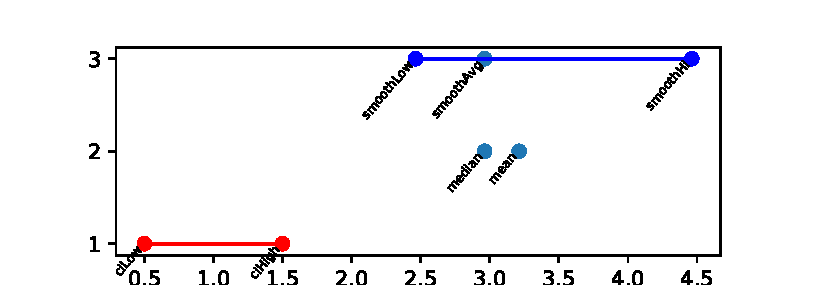
\includegraphics[width=0.7\linewidth]{illustrations/conf}
\caption{}
\label{fig:conf}
\end{figure}


Pour les itérations 26, 27,  etc. Nous allons présenter les détails de l'itération, le graphique reprenant les deux intervalles de confiance ainsi que la moyenne et la médiane et enfin la détection des alarmes.

\begin{table}[H]
	\centering
	\rowcolors{1}{ligntrose}{lightgray}
	\begin{tabularx}{\textwidth}{lX}
		\textbf{Itération}&26 \\
		\textbf{timeWindow}& 2018-01-02 02:04:21 \\
		\textbf{median} &[2.9630000000000005, 2.9630000000000005, 2.9630000000000005, 2.9630000000000005, 2.9630000000000005, 2.9630000000000005, 2.9630000000000005, 2.9630000000000005, 2.9630000000000005, 2.9630000000000005, 2.9630000000000005, 2.9630000000000005, 2.9630000000000005, 2.9630000000000005, 2.9630000000000005, 2.9630000000000005, 2.9630000000000005, 2.9630000000000005, 2.9630000000000005, 2.9630000000000005, 2.9630000000000005, 2.9630000000000005, 2.9630000000000005, 2.9630000000000005, 2.9630000000000005, 10823.963] \\
		\textbf{mean} & [3.2130000000000005, 3.2130000000000005, 3.2130000000000005, 3.2130000000000005, 3.2130000000000005, 3.2130000000000005, 3.2130000000000005, 3.2130000000000005, 3.2130000000000005, 3.2130000000000005, 3.2130000000000005, 3.2130000000000005, 3.2130000000000005, 3.2130000000000005, 3.2130000000000005, 3.2130000000000005, 3.2130000000000005, 3.2130000000000005, 3.2130000000000005, 3.2130000000000005, 3.2130000000000005, 3.2130000000000005, 3.2130000000000005, 3.2130000000000005, 3.2130000000000005, 10832.213] \\
		\textbf{ciLow}& [0.5, 0.5, 0.5, 0.5, 0.5, 0.5, 0.5, 0.5, 0.5, 0.5, 0.5, 0.5, 0.5, 0.5, 0.5, 0.5, 0.5, 0.5, 0.5, 0.5, 0.5, 0.5, 0.5, 0.5, 0.5, 142.5] \\
		\textbf{ciHigh}& [1.5000000000000004, 1.5000000000000004, 1.5000000000000004, 1.5000000000000004, 1.5000000000000004, 1.5000000000000004, 1.5000000000000004, 1.5000000000000004, 1.5000000000000004, 1.5000000000000004, 1.5000000000000004, 1.5000000000000004, 1.5000000000000004, 1.5000000000000004, 1.5000000000000004, 1.5000000000000004, 1.5000000000000004, 1.5000000000000004, 1.5000000000000004, 1.5000000000000004, 1.5000000000000004, 1.5000000000000004, 1.5000000000000004, 1.5000000000000004, 1.5000000000000004, 175.5] \\
		
			\end{tabularx} 
		\end{table}
		
		\begin{table}[H]
			\centering
			\rowcolors{1}{ligntrose}{lightgray}
			\begin{tabularx}{\textwidth}{lX}
		  \textbf{smoothAvg}&  [2.9630000000000005, 2.9630000000000005, 2.9630000000000005, 2.9630000000000005, 2.9630000000000005, 2.9630000000000005, 2.9630000000000005, 2.9630000000000005, 2.9630000000000005, 2.9630000000000005, 2.9630000000000005, 2.9630000000000005, 2.9630000000000005, 2.9630000000000005, 2.9630000000000005, 2.9630000000000005, 2.9630000000000005, 2.9630000000000005, 2.9630000000000005, 2.9630000000000005, 2.9630000000000005, 2.9630000000000005, 2.9630000000000005, 2.9630000000000005, 2.9630000000000005, 111.173] \\
		\textbf{smoothHi}& [4.463000000000001, 4.463000000000001, 4.463000000000001, 4.463000000000001, 4.463000000000001, 4.463000000000001, 4.463000000000001, 4.463000000000001, 4.463000000000001, 4.463000000000001, 4.463000000000001, 4.463000000000001, 4.463000000000001, 4.463000000000001, 4.463000000000001, 4.463000000000001, 4.463000000000001, 4.463000000000001, 4.463000000000001, 4.463000000000001, 4.463000000000001, 4.463000000000001, 4.463000000000001, 4.463000000000001, 4.463000000000001, 114.413] \\
		\textbf{smoothLow} &[2.4630000000000005, 2.4630000000000005, 2.4630000000000005, 2.4630000000000005, 2.4630000000000005, 2.4630000000000005, 2.4630000000000005, 2.4630000000000005, 2.4630000000000005, 2.4630000000000005, 2.4630000000000005, 2.4630000000000005, 2.4630000000000005, 2.4630000000000005, 2.4630000000000005, 2.4630000000000005, 2.4630000000000005, 2.4630000000000005, 2.4630000000000005, 2.4630000000000005, 2.4630000000000005, 2.4630000000000005, 2.4630000000000005, 2.4630000000000005, 2.4630000000000005, 109.253]\\
		
	\end{tabularx} 
\end{table}



\begin{figure}[]
\centering
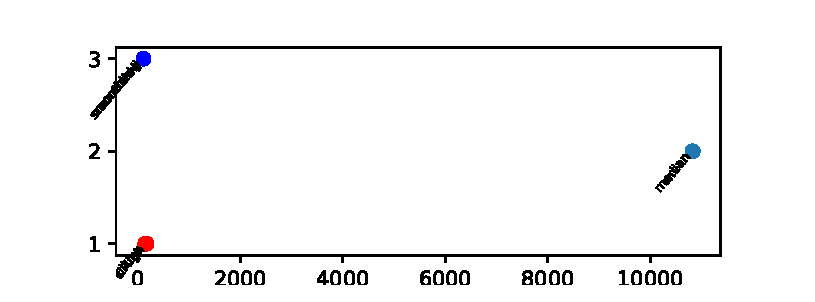
\includegraphics[width=1\linewidth]{illustrations/2018-01-0202:04:21}
\caption{}
\label{fig:2018-01-0202:04:21}
\end{figure}

La détection : 
\begin{lstlisting}[language=python,numbers=left,
frame=single,
showstringspaces=true,
basicstyle=\footnotesize,
keywordstyle=\color{blue}\ttfamily\textbf,
identifierstyle=\color{magenta}\ttfamily,
stringstyle=\color{red}\ttfamily,
commentstyle=\color{cyan}\ttfamily\textit
]

condition 1 : (median[-1] , ciLow[-1], median[-1] - ciLow[-1], >, smoothHi[-1])
( 10823.963 , 142.5, 10681.463, '>', 114.413)

condition 2 : (median[-1] , ciHigh[-1], median[-1] + ciHigh[-1] < smoothLow[-1])
(10823.963, 175.5, 10999.463, '<', 109.253)

condition 3 :(median[-1] , smoothAvg[-1],  abs(median[-1] - smoothAvg[-1]), >, 1)
(10823.963, 111.173, 10712.789999999999, '>', 1)
\end{lstlisting}

Une anomalie est détectée car condition 1 AND condition 3 = True. Rappelons qu'un anomalie est détectée si :

(condition 1 OR condition 2) AND condition 3 = True.




\begin{table}[H]
	\centering
	\rowcolors{1}{ligntrose}{lightgray}
	\begin{tabularx}{\textwidth}{lX}
		\textbf{Itération}& 27 \\
		\textbf{timeWindow}& 2018-01-02 03:04:21 \\
		
		\textbf{median}& [2.9630000000000005, 2.9630000000000005, 2.9630000000000005, 2.9630000000000005, 2.9630000000000005, 2.9630000000000005, 2.9630000000000005, 2.9630000000000005, 2.9630000000000005, 2.9630000000000005, 2.9630000000000005, 2.9630000000000005, 2.9630000000000005, 2.9630000000000005, 2.9630000000000005, 2.9630000000000005, 2.9630000000000005, 2.9630000000000005, 2.9630000000000005, 2.9630000000000005, 2.9630000000000005, 2.9630000000000005, 2.9630000000000005, 2.9630000000000005, 2.9630000000000005, 10823.963, 1071.463] \\
		\textbf{mean} & [3.2130000000000005, 3.2130000000000005, 3.2130000000000005, 3.2130000000000005, 3.2130000000000005, 3.2130000000000005, 3.2130000000000005, 3.2130000000000005, 3.2130000000000005, 3.2130000000000005, 3.2130000000000005, 3.2130000000000005, 3.2130000000000005, 3.2130000000000005, 3.2130000000000005, 3.2130000000000005, 3.2130000000000005, 3.2130000000000005, 3.2130000000000005, 3.2130000000000005, 3.2130000000000005, 3.2130000000000005, 3.2130000000000005, 3.2130000000000005, 3.2130000000000005, 10832.213, 1072.213] \\
		\textbf{ciLow}& [0.5, 0.5, 0.5, 0.5, 0.5, 0.5, 0.5, 0.5, 0.5, 0.5, 0.5, 0.5, 0.5, 0.5, 0.5, 0.5, 0.5, 0.5, 0.5, 0.5, 0.5, 0.5, 0.5, 0.5, 0.5, 142.5, 25.0] \\
		\textbf{ciHigh}& [1.5000000000000004, 1.5000000000000004, 1.5000000000000004, 1.5000000000000004, 1.5000000000000004, 1.5000000000000004, 1.5000000000000004, 1.5000000000000004, 1.5000000000000004, 1.5000000000000004, 1.5000000000000004, 1.5000000000000004, 1.5000000000000004, 1.5000000000000004, 1.5000000000000004, 1.5000000000000004, 1.5000000000000004, 1.5000000000000004, 1.5000000000000004, 1.5000000000000004, 1.5000000000000004, 1.5000000000000004, 1.5000000000000004, 1.5000000000000004, 1.5000000000000004, 175.5, 28.0] \\
							\end{tabularx} 
						\end{table}
						
						\begin{table}[H]
							\centering
							\rowcolors{1}{ligntrose}{lightgray}
							\begin{tabularx}{\textwidth}{lX}
		\textbf{smoothAvg}&  [2.9630000000000005, 2.9630000000000005, 2.9630000000000005, 2.9630000000000005, 2.9630000000000005, 2.9630000000000005, 2.9630000000000005, 2.9630000000000005, 2.9630000000000005, 2.9630000000000005, 2.9630000000000005, 2.9630000000000005, 2.9630000000000005, 2.9630000000000005, 2.9630000000000005, 2.9630000000000005, 2.9630000000000005, 2.9630000000000005, 2.9630000000000005, 2.9630000000000005, 2.9630000000000005, 2.9630000000000005, 2.9630000000000005, 2.9630000000000005, 2.9630000000000005, 111.173, 120.77590000000001] \\
		\textbf{smoothHi}& [4.463000000000001, 4.463000000000001, 4.463000000000001, 4.463000000000001, 4.463000000000001, 4.463000000000001, 4.463000000000001, 4.463000000000001, 4.463000000000001, 4.463000000000001, 4.463000000000001, 4.463000000000001, 4.463000000000001, 4.463000000000001, 4.463000000000001, 4.463000000000001, 4.463000000000001, 4.463000000000001, 4.463000000000001, 4.463000000000001, 4.463000000000001, 4.463000000000001, 4.463000000000001, 4.463000000000001, 4.463000000000001, 114.413, 124.2635] \\
		\textbf{smoothLow} &[2.4630000000000005, 2.4630000000000005, 2.4630000000000005, 2.4630000000000005, 2.4630000000000005, 2.4630000000000005, 2.4630000000000005, 2.4630000000000005, 2.4630000000000005, 2.4630000000000005, 2.4630000000000005, 2.4630000000000005, 2.4630000000000005, 2.4630000000000005, 2.4630000000000005, 2.4630000000000005, 2.4630000000000005, 2.4630000000000005, 2.4630000000000005, 2.4630000000000005, 2.4630000000000005, 2.4630000000000005, 2.4630000000000005, 2.4630000000000005, 2.4630000000000005, 109.253, 118.6251]\\
	\end{tabularx} 
\end{table}

Les intervalles de confiance, la moyenne et la médiane: 
\begin{figure}[H]
\centering
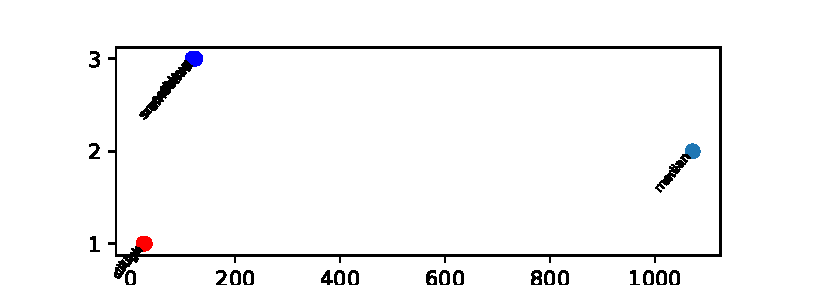
\includegraphics[width=1\linewidth]{illustrations/2018-01-0203:04:21-}
\caption{}
\label{fig:2018-01-0203:04:21-}
\end{figure}

La détection :

\begin{lstlisting}[language=python,numbers=left,
frame=single,
showstringspaces=true,
basicstyle=\footnotesize,
keywordstyle=\color{blue}\ttfamily\textbf,
identifierstyle=\color{magenta}\ttfamily,
stringstyle=\color{red}\ttfamily,
commentstyle=\color{cyan}\ttfamily\textit
]

(median[-1] , ciLow[-1], median[-1] - ciLow[-1] > smoothHi[-1])
(1071.463, 25.0, 1046.463, '>', 124.2635)

(median[-1] + ciHigh[-1] < smoothLow[-1])
( 1071.463, 28.0, 1099.463, '<', 118.6251)

(abs(median[-1] - smoothAvg[-1]) > 1)
1071.463, 120.77590000000001, 950.6871, '>', 1)
\end{lstlisting}


\begin{table}[H]
	\centering
	\rowcolors{1}{ligntrose}{lightgray}
	\begin{tabularx}{\textwidth}{lX}
		\textbf{Itération}& 28\\
		\textbf{timeWindow}& 2018-01-02 04:04:21 \\
		
		\textbf{median}& [2.9630000000000005, 2.9630000000000005, 2.9630000000000005, 2.9630000000000005, 2.9630000000000005, 2.9630000000000005, 2.9630000000000005, 2.9630000000000005, 2.9630000000000005, 2.9630000000000005, 2.9630000000000005, 2.9630000000000005, 2.9630000000000005, 2.9630000000000005, 2.9630000000000005, 2.9630000000000005, 2.9630000000000005, 2.9630000000000005, 2.9630000000000005, 2.9630000000000005, 2.9630000000000005, 2.9630000000000005, 2.9630000000000005, 2.9630000000000005, 2.9630000000000005, 10823.963, 1071.463, 1071.463]\\ 
		\textbf{mean} & [3.2130000000000005, 3.2130000000000005, 3.2130000000000005, 3.2130000000000005, 3.2130000000000005, 3.2130000000000005, 3.2130000000000005, 3.2130000000000005, 3.2130000000000005, 3.2130000000000005, 3.2130000000000005, 3.2130000000000005, 3.2130000000000005, 3.2130000000000005, 3.2130000000000005, 3.2130000000000005, 3.2130000000000005, 3.2130000000000005, 3.2130000000000005, 3.2130000000000005, 3.2130000000000005, 3.2130000000000005, 3.2130000000000005, 3.2130000000000005, 3.2130000000000005, 10832.213, 1072.213, 1072.213]\\ 
		\textbf{ciLow}& [0.5, 0.5, 0.5, 0.5, 0.5, 0.5, 0.5, 0.5, 0.5, 0.5, 0.5, 0.5, 0.5, 0.5, 0.5, 0.5, 0.5, 0.5, 0.5, 0.5, 0.5, 0.5, 0.5, 0.5, 0.5, 142.5, 25.0, 25.0] \\
		\textbf{ciHigh}& [1.5000000000000004, 1.5000000000000004, 1.5000000000000004, 1.5000000000000004, 1.5000000000000004, 1.5000000000000004, 1.5000000000000004, 1.5000000000000004, 1.5000000000000004, 1.5000000000000004, 1.5000000000000004, 1.5000000000000004, 1.5000000000000004, 1.5000000000000004, 1.5000000000000004, 1.5000000000000004, 1.5000000000000004, 1.5000000000000004, 1.5000000000000004, 1.5000000000000004, 1.5000000000000004, 1.5000000000000004, 1.5000000000000004, 1.5000000000000004, 1.5000000000000004, 175.5, 28.0, 28.0] \\
		
					\end{tabularx} 
				\end{table}
				
				\begin{table}[H]
					\centering
					\rowcolors{1}{ligntrose}{lightgray}
					\begin{tabularx}{\textwidth}{lX}
		\textbf{smoothAvg}&  [2.9630000000000005, 2.9630000000000005, 2.9630000000000005, 2.9630000000000005, 2.9630000000000005, 2.9630000000000005, 2.9630000000000005, 2.9630000000000005, 2.9630000000000005, 2.9630000000000005, 2.9630000000000005, 2.9630000000000005, 2.9630000000000005, 2.9630000000000005, 2.9630000000000005, 2.9630000000000005, 2.9630000000000005, 2.9630000000000005, 2.9630000000000005, 2.9630000000000005, 2.9630000000000005, 2.9630000000000005, 2.9630000000000005, 2.9630000000000005, 2.9630000000000005, 111.173, 120.77590000000001, 130.28277100000003] \\
		\textbf{smoothHi}& [4.463000000000001, 4.463000000000001, 4.463000000000001, 4.463000000000001, 4.463000000000001, 4.463000000000001, 4.463000000000001, 4.463000000000001, 4.463000000000001, 4.463000000000001, 4.463000000000001, 4.463000000000001, 4.463000000000001, 4.463000000000001, 4.463000000000001, 4.463000000000001, 4.463000000000001, 4.463000000000001, 4.463000000000001, 4.463000000000001, 4.463000000000001, 4.463000000000001, 4.463000000000001, 4.463000000000001, 4.463000000000001, 114.413, 124.2635, 134.015495] \\
		\textbf{smoothLow} &[2.4630000000000005, 2.4630000000000005, 2.4630000000000005, 2.4630000000000005, 2.4630000000000005, 2.4630000000000005, 2.4630000000000005, 2.4630000000000005, 2.4630000000000005, 2.4630000000000005, 2.4630000000000005, 2.4630000000000005, 2.4630000000000005, 2.4630000000000005, 2.4630000000000005, 2.4630000000000005, 2.4630000000000005, 2.4630000000000005, 2.4630000000000005, 2.4630000000000005, 2.4630000000000005, 2.4630000000000005, 2.4630000000000005, 2.4630000000000005, 2.4630000000000005, 109.253, 118.6251, 127.903479]\\
		
		
	\end{tabularx} 
\end{table}

\begin{table}[H]
	\centering
	\rowcolors{1}{ligntrose}{lightgray}
	\begin{tabularx}{\textwidth}{lX}
		\textbf{Itération}& 29 \\
		\textbf{timeWindow} &2018-01-02 05:04:21 \\
		
		\textbf{median} &[2.9630000000000005, 2.9630000000000005, 2.9630000000000005, 2.9630000000000005, 2.9630000000000005, 2.9630000000000005, 2.9630000000000005, 2.9630000000000005, 2.9630000000000005, 2.9630000000000005, 2.9630000000000005, 2.9630000000000005, 2.9630000000000005, 2.9630000000000005, 2.9630000000000005, 2.9630000000000005, 2.9630000000000005, 2.9630000000000005, 2.9630000000000005, 2.9630000000000005, 2.9630000000000005, 2.9630000000000005, 2.9630000000000005, 2.9630000000000005, 2.9630000000000005, 10823.963, 1071.463, 1071.463, 2.9630000000000005] \\
		\textbf{mean} & [3.2130000000000005, 3.2130000000000005, 3.2130000000000005, 3.2130000000000005, 3.2130000000000005, 3.2130000000000005, 3.2130000000000005, 3.2130000000000005, 3.2130000000000005, 3.2130000000000005, 3.2130000000000005, 3.2130000000000005, 3.2130000000000005, 3.2130000000000005, 3.2130000000000005, 3.2130000000000005, 3.2130000000000005, 3.2130000000000005, 3.2130000000000005, 3.2130000000000005, 3.2130000000000005, 3.2130000000000005, 3.2130000000000005, 3.2130000000000005, 3.2130000000000005, 10832.213, 1072.213, 1072.213, 3.2130000000000005] \\
		\textbf{ciLow}& [0.5, 0.5, 0.5, 0.5, 0.5, 0.5, 0.5, 0.5, 0.5, 0.5, 0.5, 0.5, 0.5, 0.5, 0.5, 0.5, 0.5, 0.5, 0.5, 0.5, 0.5, 0.5, 0.5, 0.5, 0.5, 142.5, 25.0, 25.0, 0.5] \\
		\textbf{ciHigh}& [1.5000000000000004, 1.5000000000000004, 1.5000000000000004, 1.5000000000000004, 1.5000000000000004, 1.5000000000000004, 1.5000000000000004, 1.5000000000000004, 1.5000000000000004, 1.5000000000000004, 1.5000000000000004, 1.5000000000000004, 1.5000000000000004, 1.5000000000000004, 1.5000000000000004, 1.5000000000000004, 1.5000000000000004, 1.5000000000000004, 1.5000000000000004, 1.5000000000000004, 1.5000000000000004, 1.5000000000000004, 1.5000000000000004, 1.5000000000000004, 1.5000000000000004, 175.5, 28.0, 28.0, 1.5000000000000004] \\
							\end{tabularx} 
						\end{table}
						
						\begin{table}[H]
							\centering
							\rowcolors{1}{ligntrose}{lightgray}
							\begin{tabularx}{\textwidth}{lX}
		\textbf{smoothAvg}&  [2.9630000000000005, 2.9630000000000005, 2.9630000000000005, 2.9630000000000005, 2.9630000000000005, 2.9630000000000005, 2.9630000000000005, 2.9630000000000005, 2.9630000000000005, 2.9630000000000005, 2.9630000000000005, 2.9630000000000005, 2.9630000000000005, 2.9630000000000005, 2.9630000000000005, 2.9630000000000005, 2.9630000000000005, 2.9630000000000005, 2.9630000000000005, 2.9630000000000005, 2.9630000000000005, 2.9630000000000005, 2.9630000000000005, 2.9630000000000005, 2.9630000000000005, 111.173, 120.77590000000001, 130.28277100000003, 129.00957329000002] \\
		\textbf{smoothHi}& [4.463000000000001, 4.463000000000001, 4.463000000000001, 4.463000000000001, 4.463000000000001, 4.463000000000001, 4.463000000000001, 4.463000000000001, 4.463000000000001, 4.463000000000001, 4.463000000000001, 4.463000000000001, 4.463000000000001, 4.463000000000001, 4.463000000000001, 4.463000000000001, 4.463000000000001, 4.463000000000001, 4.463000000000001, 4.463000000000001, 4.463000000000001, 4.463000000000001, 4.463000000000001, 4.463000000000001, 4.463000000000001, 114.413, 124.2635, 134.015495, 132.71997005] \\
		\textbf{smoothLow} &[2.4630000000000005, 2.4630000000000005, 2.4630000000000005, 2.4630000000000005, 2.4630000000000005, 2.4630000000000005, 2.4630000000000005, 2.4630000000000005, 2.4630000000000005, 2.4630000000000005, 2.4630000000000005, 2.4630000000000005, 2.4630000000000005, 2.4630000000000005, 2.4630000000000005, 2.4630000000000005, 2.4630000000000005, 2.4630000000000005, 2.4630000000000005, 2.4630000000000005, 2.4630000000000005, 2.4630000000000005, 2.4630000000000005, 2.4630000000000005, 2.4630000000000005, 109.253, 118.6251, 127.903479, 126.64907421000001]\\
		
		
	\end{tabularx} 
\end{table}

\begin{table}[H]
	\centering
	\rowcolors{1}{ligntrose}{lightgray}
	\begin{tabularx}{\textwidth}{lX}
		\textbf{Itération}& 30\\
		\textbf{timeWindow} &2018-01-02 06:04:21 \\ 
		\textbf{median} &[2.9630000000000005, 2.9630000000000005, 2.9630000000000005, 2.9630000000000005, 2.9630000000000005, 2.9630000000000005, 2.9630000000000005, 2.9630000000000005, 2.9630000000000005, 2.9630000000000005, 2.9630000000000005, 2.9630000000000005, 2.9630000000000005, 2.9630000000000005, 2.9630000000000005, 2.9630000000000005, 2.9630000000000005, 2.9630000000000005, 2.9630000000000005, 2.9630000000000005, 2.9630000000000005, 2.9630000000000005, 2.9630000000000005, 2.9630000000000005, 2.9630000000000005, 10823.963, 1071.463, 1071.463, 2.9630000000000005, 2.9630000000000005]\\ 
		\textbf{mean} & [3.2130000000000005, 3.2130000000000005, 3.2130000000000005, 3.2130000000000005, 3.2130000000000005, 3.2130000000000005, 3.2130000000000005, 3.2130000000000005, 3.2130000000000005, 3.2130000000000005, 3.2130000000000005, 3.2130000000000005, 3.2130000000000005, 3.2130000000000005, 3.2130000000000005, 3.2130000000000005, 3.2130000000000005, 3.2130000000000005, 3.2130000000000005, 3.2130000000000005, 3.2130000000000005, 3.2130000000000005, 3.2130000000000005, 3.2130000000000005, 3.2130000000000005, 10832.213, 1072.213, 1072.213, 3.2130000000000005, 3.2130000000000005]\\ 
		\textbf{ciLow}& [0.5, 0.5, 0.5, 0.5, 0.5, 0.5, 0.5, 0.5, 0.5, 0.5, 0.5, 0.5, 0.5, 0.5, 0.5, 0.5, 0.5, 0.5, 0.5, 0.5, 0.5, 0.5, 0.5, 0.5, 0.5, 142.5, 25.0, 25.0, 0.5, 0.5] \\
		\textbf{ciHigh}& [1.5000000000000004, 1.5000000000000004, 1.5000000000000004, 1.5000000000000004, 1.5000000000000004, 1.5000000000000004, 1.5000000000000004, 1.5000000000000004, 1.5000000000000004, 1.5000000000000004, 1.5000000000000004, 1.5000000000000004, 1.5000000000000004, 1.5000000000000004, 1.5000000000000004, 1.5000000000000004, 1.5000000000000004, 1.5000000000000004, 1.5000000000000004, 1.5000000000000004, 1.5000000000000004, 1.5000000000000004, 1.5000000000000004, 1.5000000000000004, 1.5000000000000004, 175.5, 28.0, 28.0, 1.5000000000000004, 1.5000000000000004] \\
							\end{tabularx} 
						\end{table}
						
						\begin{table}[H]
							\centering
							\rowcolors{1}{ligntrose}{lightgray}
							\begin{tabularx}{\textwidth}{lX}
		\textbf{smoothAvg}&  [2.9630000000000005, 2.9630000000000005, 2.9630000000000005, 2.9630000000000005, 2.9630000000000005, 2.9630000000000005, 2.9630000000000005, 2.9630000000000005, 2.9630000000000005, 2.9630000000000005, 2.9630000000000005, 2.9630000000000005, 2.9630000000000005, 2.9630000000000005, 2.9630000000000005, 2.9630000000000005, 2.9630000000000005, 2.9630000000000005, 2.9630000000000005, 2.9630000000000005, 2.9630000000000005, 2.9630000000000005, 2.9630000000000005, 2.9630000000000005, 2.9630000000000005, 111.173, 120.77590000000001, 130.28277100000003, 129.00957329000002, 127.74910755710002] \\
		\textbf{smoothHi}& [4.463000000000001, 4.463000000000001, 4.463000000000001, 4.463000000000001, 4.463000000000001, 4.463000000000001, 4.463000000000001, 4.463000000000001, 4.463000000000001, 4.463000000000001, 4.463000000000001, 4.463000000000001, 4.463000000000001, 4.463000000000001, 4.463000000000001, 4.463000000000001, 4.463000000000001, 4.463000000000001, 4.463000000000001, 4.463000000000001, 4.463000000000001, 4.463000000000001, 4.463000000000001, 4.463000000000001, 4.463000000000001, 114.413, 124.2635, 134.015495, 132.71997005, 131.43740034950002] \\
		\textbf{smoothLow} &[2.4630000000000005, 2.4630000000000005, 2.4630000000000005, 2.4630000000000005, 2.4630000000000005, 2.4630000000000005, 2.4630000000000005, 2.4630000000000005, 2.4630000000000005, 2.4630000000000005, 2.4630000000000005, 2.4630000000000005, 2.4630000000000005, 2.4630000000000005, 2.4630000000000005, 2.4630000000000005, 2.4630000000000005, 2.4630000000000005, 2.4630000000000005, 2.4630000000000005, 2.4630000000000005, 2.4630000000000005, 2.4630000000000005, 2.4630000000000005, 2.4630000000000005, 109.253, 118.6251, 127.903479, 126.64907421000001, 125.40721346790001]\\
		
	\end{tabularx} 
\end{table}
\begin{table}[H]
	\centering
	\rowcolors{1}{ligntrose}{lightgray}
	\begin{tabularx}{\textwidth}{lX}
		\textbf{Itération}& 31\\
		\textbf{timeWindow} &2018-01-02 07:04:21 \\
		
		\textbf{median}& [2.9630000000000005, 2.9630000000000005, 2.9630000000000005, 2.9630000000000005, 2.9630000000000005, 2.9630000000000005, 2.9630000000000005, 2.9630000000000005, 2.9630000000000005, 2.9630000000000005, 2.9630000000000005, 2.9630000000000005, 2.9630000000000005, 2.9630000000000005, 2.9630000000000005, 2.9630000000000005, 2.9630000000000005, 2.9630000000000005, 2.9630000000000005, 2.9630000000000005, 2.9630000000000005, 2.9630000000000005, 2.9630000000000005, 2.9630000000000005, 2.9630000000000005, 10823.963, 1071.463, 1071.463, 2.9630000000000005, 2.9630000000000005, 2.9630000000000005] \\
		\textbf{mean} & [3.2130000000000005, 3.2130000000000005, 3.2130000000000005, 3.2130000000000005, 3.2130000000000005, 3.2130000000000005, 3.2130000000000005, 3.2130000000000005, 3.2130000000000005, 3.2130000000000005, 3.2130000000000005, 3.2130000000000005, 3.2130000000000005, 3.2130000000000005, 3.2130000000000005, 3.2130000000000005, 3.2130000000000005, 3.2130000000000005, 3.2130000000000005, 3.2130000000000005, 3.2130000000000005, 3.2130000000000005, 3.2130000000000005, 3.2130000000000005, 3.2130000000000005, 10832.213, 1072.213, 1072.213, 3.2130000000000005, 3.2130000000000005, 3.2130000000000005] \\
		\textbf{ciLow}& [0.5, 0.5, 0.5, 0.5, 0.5, 0.5, 0.5, 0.5, 0.5, 0.5, 0.5, 0.5, 0.5, 0.5, 0.5, 0.5, 0.5, 0.5, 0.5, 0.5, 0.5, 0.5, 0.5, 0.5, 0.5, 142.5, 25.0, 25.0, 0.5, 0.5, 0.5]\\ 
							\end{tabularx} 
						\end{table}
						
						\begin{table}[H]
							\centering
							\rowcolors{1}{ligntrose}{lightgray}
							\begin{tabularx}{\textwidth}{lX}
		\textbf{ciHigh}& [1.5000000000000004, 1.5000000000000004, 1.5000000000000004, 1.5000000000000004, 1.5000000000000004, 1.5000000000000004, 1.5000000000000004, 1.5000000000000004, 1.5000000000000004, 1.5000000000000004, 1.5000000000000004, 1.5000000000000004, 1.5000000000000004, 1.5000000000000004, 1.5000000000000004, 1.5000000000000004, 1.5000000000000004, 1.5000000000000004, 1.5000000000000004, 1.5000000000000004, 1.5000000000000004, 1.5000000000000004, 1.5000000000000004, 1.5000000000000004, 1.5000000000000004, 175.5, 28.0, 28.0, 1.5000000000000004, 1.5000000000000004, 1.5000000000000004]\\ 
		\textbf{smoothAvg}&  [2.9630000000000005, 2.9630000000000005, 2.9630000000000005, 2.9630000000000005, 2.9630000000000005, 2.9630000000000005, 2.9630000000000005, 2.9630000000000005, 2.9630000000000005, 2.9630000000000005, 2.9630000000000005, 2.9630000000000005, 2.9630000000000005, 2.9630000000000005, 2.9630000000000005, 2.9630000000000005, 2.9630000000000005, 2.9630000000000005, 2.9630000000000005, 2.9630000000000005, 2.9630000000000005, 2.9630000000000005, 2.9630000000000005, 2.9630000000000005, 2.9630000000000005, 111.173, 120.77590000000001, 130.28277100000003, 129.00957329000002, 127.74910755710002, 126.50124648152901] \\
		\textbf{smoothHi}& [4.463000000000001, 4.463000000000001, 4.463000000000001, 4.463000000000001, 4.463000000000001, 4.463000000000001, 4.463000000000001, 4.463000000000001, 4.463000000000001, 4.463000000000001, 4.463000000000001, 4.463000000000001, 4.463000000000001, 4.463000000000001, 4.463000000000001, 4.463000000000001, 4.463000000000001, 4.463000000000001, 4.463000000000001, 4.463000000000001, 4.463000000000001, 4.463000000000001, 4.463000000000001, 4.463000000000001, 4.463000000000001, 114.413, 124.2635, 134.015495, 132.71997005, 131.43740034950002, 130.16765634600503] \\
		\textbf{smoothLow} &[2.4630000000000005, 2.4630000000000005, 2.4630000000000005, 2.4630000000000005, 2.4630000000000005, 2.4630000000000005, 2.4630000000000005, 2.4630000000000005, 2.4630000000000005, 2.4630000000000005, 2.4630000000000005, 2.4630000000000005, 2.4630000000000005, 2.4630000000000005, 2.4630000000000005, 2.4630000000000005, 2.4630000000000005, 2.4630000000000005, 2.4630000000000005, 2.4630000000000005, 2.4630000000000005, 2.4630000000000005, 2.4630000000000005, 2.4630000000000005, 2.4630000000000005, 109.253, 118.6251, 127.903479, 126.64907421000001, 125.40721346790001, 124.177771333221]\\
		
	\end{tabularx} 
\end{table}

\begin{table}[H]
	\centering
	\rowcolors{1}{ligntrose}{lightgray}
	\begin{tabularx}{\textwidth}{lX}
		\textbf{Itération}& 32\\
		\textbf{timeWindow}& 2018-01-02 07:04:21 \\
		\textbf{median}& [2.9630000000000005, 2.9630000000000005, 2.9630000000000005, 2.9630000000000005, 2.9630000000000005, 2.9630000000000005, 2.9630000000000005, 2.9630000000000005, 2.9630000000000005, 2.9630000000000005, 2.9630000000000005, 2.9630000000000005, 2.9630000000000005, 2.9630000000000005, 2.9630000000000005, 2.9630000000000005, 2.9630000000000005, 2.9630000000000005, 2.9630000000000005, 2.9630000000000005, 2.9630000000000005, 2.9630000000000005, 2.9630000000000005, 2.9630000000000005, 2.9630000000000005, 10823.963, 1071.463, 1071.463, 2.9630000000000005, 2.9630000000000005, 2.9630000000000005] \\
		\textbf{mean} & [3.2130000000000005, 3.2130000000000005, 3.2130000000000005, 3.2130000000000005, 3.2130000000000005, 3.2130000000000005, 3.2130000000000005, 3.2130000000000005, 3.2130000000000005, 3.2130000000000005, 3.2130000000000005, 3.2130000000000005, 3.2130000000000005, 3.2130000000000005, 3.2130000000000005, 3.2130000000000005, 3.2130000000000005, 3.2130000000000005, 3.2130000000000005, 3.2130000000000005, 3.2130000000000005, 3.2130000000000005, 3.2130000000000005, 3.2130000000000005, 3.2130000000000005, 10832.213, 1072.213, 1072.213, 3.2130000000000005, 3.2130000000000005, 3.2130000000000005] \\
		\textbf{ciLow}& [0.5, 0.5, 0.5, 0.5, 0.5, 0.5, 0.5, 0.5, 0.5, 0.5, 0.5, 0.5, 0.5, 0.5, 0.5, 0.5, 0.5, 0.5, 0.5, 0.5, 0.5, 0.5, 0.5, 0.5, 0.5, 142.5, 25.0, 25.0, 0.5, 0.5, 0.5] \\
		
							\end{tabularx} 
						\end{table}
						
						\begin{table}[H]
							\centering
							\rowcolors{1}{ligntrose}{lightgray}
							\begin{tabularx}{\textwidth}{lX}
		\textbf{ciHigh}& [1.5000000000000004, 1.5000000000000004, 1.5000000000000004, 1.5000000000000004, 1.5000000000000004, 1.5000000000000004, 1.5000000000000004, 1.5000000000000004, 1.5000000000000004, 1.5000000000000004, 1.5000000000000004, 1.5000000000000004, 1.5000000000000004, 1.5000000000000004, 1.5000000000000004, 1.5000000000000004, 1.5000000000000004, 1.5000000000000004, 1.5000000000000004, 1.5000000000000004, 1.5000000000000004, 1.5000000000000004, 1.5000000000000004, 1.5000000000000004, 1.5000000000000004, 175.5, 28.0, 28.0, 1.5000000000000004, 1.5000000000000004, 1.5000000000000004] \\
		\textbf{smoothAvg}&  [2.9630000000000005, 2.9630000000000005, 2.9630000000000005, 2.9630000000000005, 2.9630000000000005, 2.9630000000000005, 2.9630000000000005, 2.9630000000000005, 2.9630000000000005, 2.9630000000000005, 2.9630000000000005, 2.9630000000000005, 2.9630000000000005, 2.9630000000000005, 2.9630000000000005, 2.9630000000000005, 2.9630000000000005, 2.9630000000000005, 2.9630000000000005, 2.9630000000000005, 2.9630000000000005, 2.9630000000000005, 2.9630000000000005, 2.9630000000000005, 2.9630000000000005, 111.173, 120.77590000000001, 130.28277100000003, 129.00957329000002, 127.74910755710002, 126.50124648152901]\\
		\textbf{smoothHi}& [4.463000000000001, 4.463000000000001, 4.463000000000001, 4.463000000000001, 4.463000000000001, 4.463000000000001, 4.463000000000001, 4.463000000000001, 4.463000000000001, 4.463000000000001, 4.463000000000001, 4.463000000000001, 4.463000000000001, 4.463000000000001, 4.463000000000001, 4.463000000000001, 4.463000000000001, 4.463000000000001, 4.463000000000001, 4.463000000000001, 4.463000000000001, 4.463000000000001, 4.463000000000001, 4.463000000000001, 4.463000000000001, 114.413, 124.2635, 134.015495, 132.71997005, 131.43740034950002, 130.16765634600503] \\
		\textbf{smoothLow} &[2.4630000000000005, 2.4630000000000005, 2.4630000000000005, 2.4630000000000005, 2.4630000000000005, 2.4630000000000005, 2.4630000000000005, 2.4630000000000005, 2.4630000000000005, 2.4630000000000005, 2.4630000000000005, 2.4630000000000005, 2.4630000000000005, 2.4630000000000005, 2.4630000000000005, 2.4630000000000005, 2.4630000000000005, 2.4630000000000005, 2.4630000000000005, 2.4630000000000005, 2.4630000000000005, 2.4630000000000005, 2.4630000000000005, 2.4630000000000005, 2.4630000000000005, 109.253, 118.6251, 127.903479, 126.64907421000001, 125.40721346790001, 124.177771333221]\\
		
	\end{tabularx} 
\end{table}




















































		\appendix
		
		\chapter{Illustration du théorème central limite} \label{appendix:clt-exemple}
		La figure \ref{fig:tcl} illustre par l'exemple le principe du TCL avec une distribution qui suit la loi normale. 
		\begin{figure}[H]
			\centering
			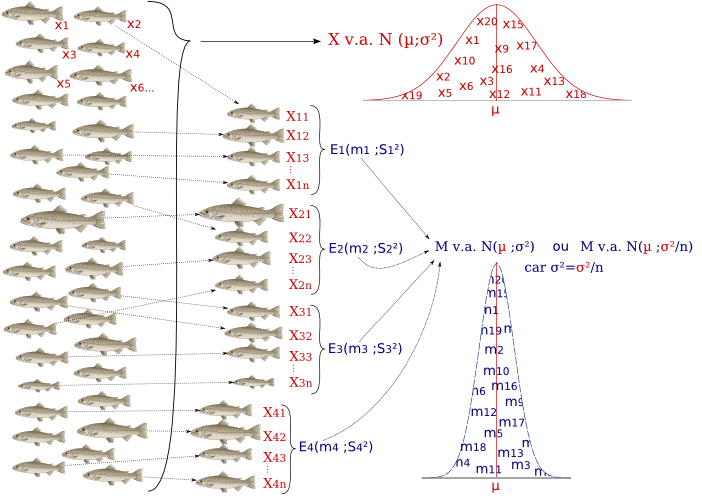
\includegraphics[width=1\linewidth]{illustrations/tcl}
			\caption{}
			\label{fig:tcl}
			\source{\url{http://webapps.fundp.ac.be/biostats/biostat/modules/module70/page4.html}, consultée le $ 28/09/2018 $.}
			
		\end{figure}
		
		
		
		
		
		
		
		
		
		
		
		
		
		
		





